\documentclass[a3paper]{article}
\usepackage[hyphens]{url}
\usepackage[utf8]{inputenc}
\usepackage[pdftex]{graphicx}
\usepackage{epstopdf}
\usepackage{amsmath}
\usepackage{amssymb}
\usepackage{mathrsfs}
\usepackage{booktabs}
\usepackage[ruled,linesnumbered]{algorithm2e}
\usepackage{cleveref}
\usepackage[misc]{ifsym}
\usepackage{longtable}
\urlstyle{same}
\usepackage[a4paper, total={7in, 10in}]{geometry}
\usepackage{amsmath}
\usepackage{amssymb}
\usepackage{cleveref}
\usepackage{booktabs}
\usepackage[switch]{lineno} 
\usepackage{ntheorem}

\usepackage{float}
\restylefloat{table}

\newtheorem{theorem}{Theorem}
\newtheorem{lemma}{Lemma}
\newtheorem*{proof}{\it{Proof.}\rm}

\newcommand{\IE}{\textit{i.e.}, }
\newcommand{\EG}{\textit{e.g.}, }
\newcommand{\ET}{\textit{et al.}}
\newcommand{\ST}{\textit{s.t.}}

\newcommand{\dd}{\mathrm{d}}
\newcommand{\vv}[1]{\bm{\mathrm{{#1}}}}
\newcommand{\E}{\operatorname{\mathbb{E}}}
\newcommand{\EE}[1]{\operatorname{\mathbb{E}}\left[{#1}\right]}
\newcommand{\EEE}[2]{\operatorname{\mathbb{E}}_{{#1}}\left[{#2}\right]}
\newcommand{\KLD}{\operatorname{KL}}
\newcommand{\KLDD}[2]{\operatorname{KL}\left[{#1}\,\big\|\,{#2}\right]}
\newcommand{\abs}[1]{\left|#1\right|}
\newcommand{\Entropy}{\operatorname{H}}
\newcommand{\Entropyy}[1]{\operatorname{H}\left[#1\right]}
\newcommand{\pin}{p_{in}}
\newcommand{\pout}{p_{out}}
\newcommand{\pmix}{p_{mix}}
\newcommand*{\QED}{\hfill\ensuremath{\square}}  %自定义,空心
% Following comment is from ijcai97-submit.tex:
% The preparation of these files was supported by Schlumberger Palo Alto
% Research, AT\&T Bell Laboratories, and Morgan Kaufmann Publishers.
% Shirley Jowell, of Morgan Kaufmann Publishers, and Peter F.
% Patel-Schneider, of AT\&T Bell Laboratories collaborated on their
% preparation.

% These instructions can be modified and used in other conferences as long
% as credit to the authors and supporting agencies is retained, this notice
% is not changed, and further modification or reuse is not restricted.
% Neither Shirley Jowell nor Peter F. Patel-Schneider can be listed as
% contacts for providing assistance without their prior permission.

% To use for other conferences, change references to files and the
% conference appropriate and use other authors, contacts, publishers, and
% organizations.
% Also change the deadline and address for returning papers and the length and
% page charge instructions.
% Put where the files are available in the appropriate places.


\title{Technique Appendix}
\begin{document}

\pagestyle{plain} 

\section{Appendix A Counter-examples}

\begin{figure}[H]
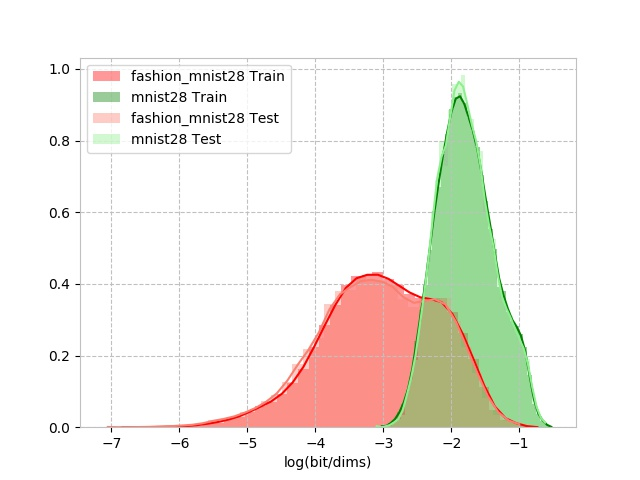
\includegraphics[width=0.5\columnwidth]{figures/log_prob_histogram}
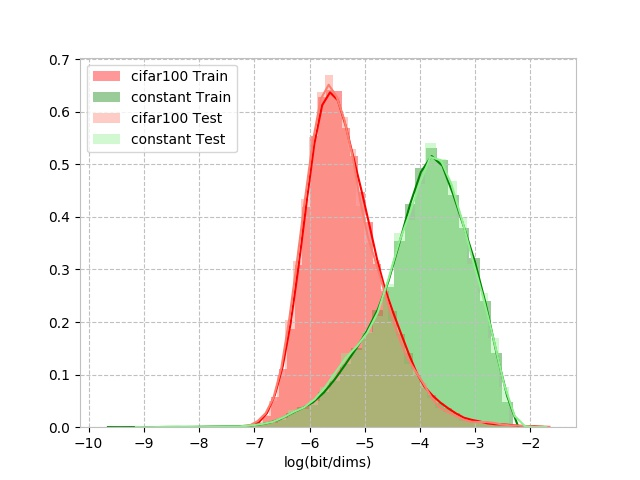
\includegraphics[width=0.5\columnwidth]{figures/log_prob_histogram-1}
\caption{Counter example of $\log p_\theta(x)$ with AUROC 0.0609 and 0.1104}
\end{figure}

\begin{figure}[H]
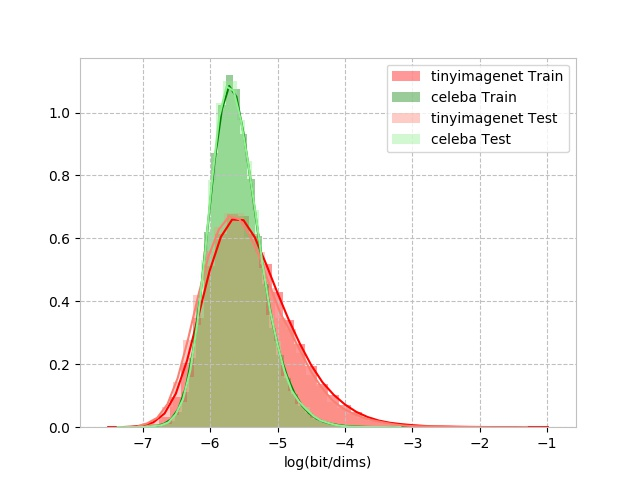
\includegraphics[width=0.5\columnwidth]{figures/log_prob_histogram-3}
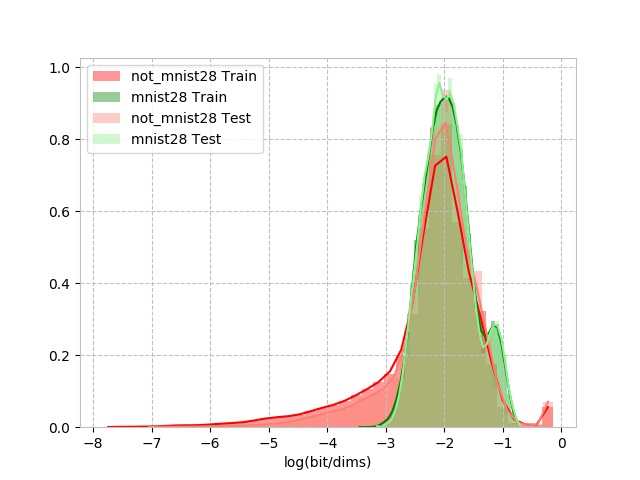
\includegraphics[width=0.5\columnwidth]{figures/log_prob_histogram-4}
\caption{Counter example of $T_{perm}(x)$ with AUROC 0.3933 and 0.4692}
\end{figure}

\begin{figure}[H]
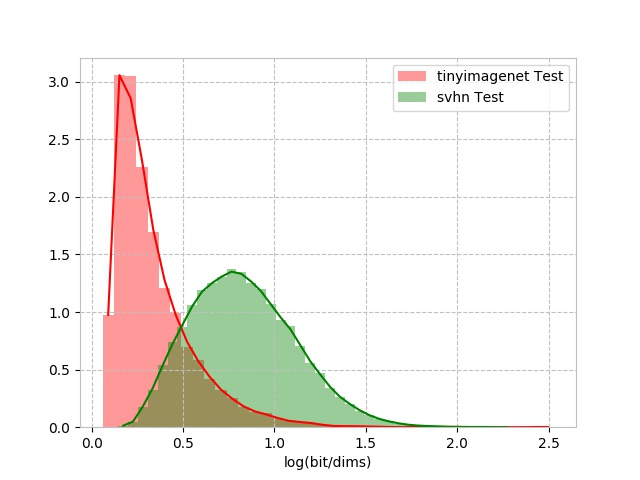
\includegraphics[width=0.5\columnwidth]{figures/grad_norm_histogram}
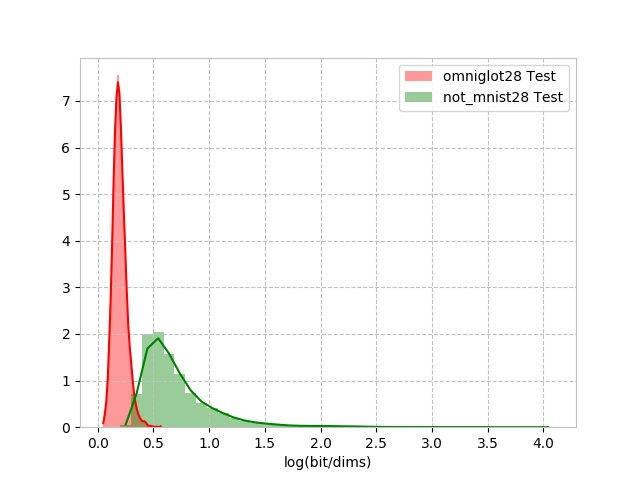
\includegraphics[width=0.5\columnwidth]{figures/grad_norm_histogram-1}
\caption{Counter example of $\|\nabla_x \log p_\theta(x)\|$ with AUROC 0.0196 and 0.0023}
\end{figure}

\begin{figure}[H]
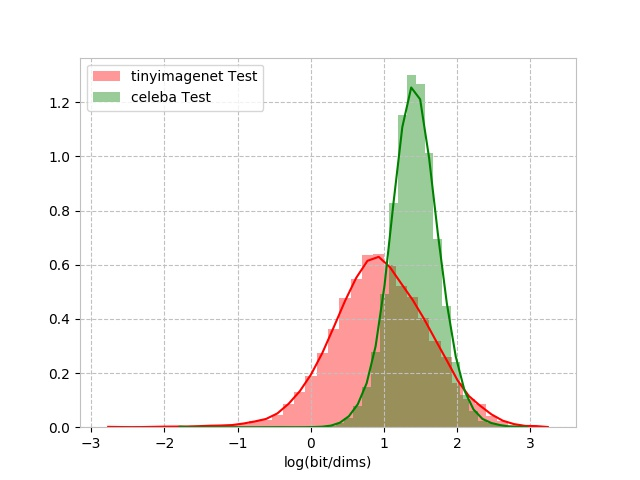
\includegraphics[width=0.5\columnwidth]{figures/ll_with_complexity_histogram}
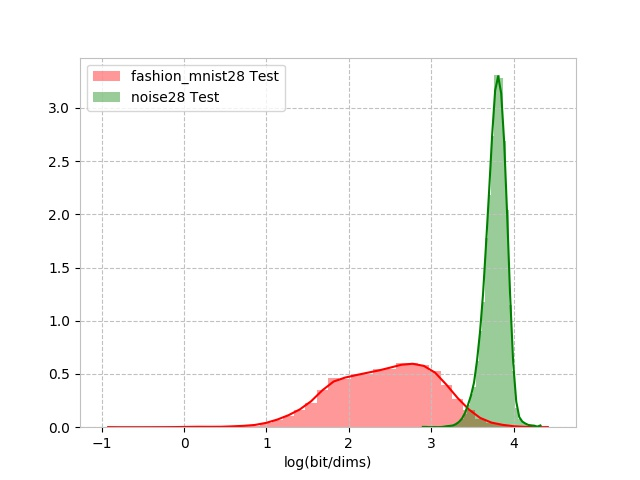
\includegraphics[width=0.5\columnwidth]{figures/ll_with_complexity_histogram-1}
\caption{Counter example of $S(x)$ with AUROC 0.2636 and 0.0062}
\end{figure}


\begin{figure}[H]
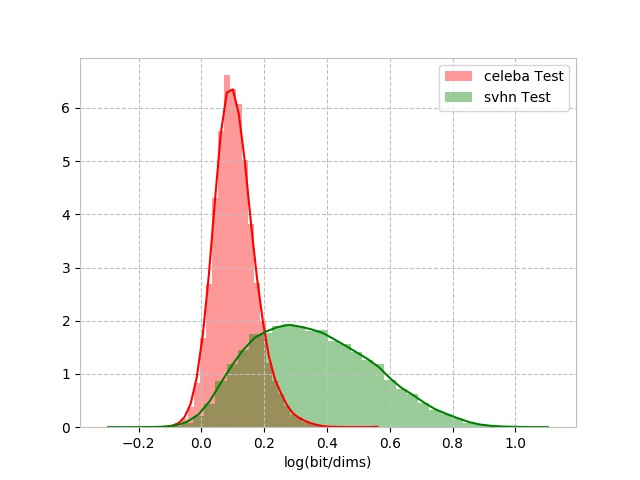
\includegraphics[width=0.5\columnwidth]{figures/kl_histogram}
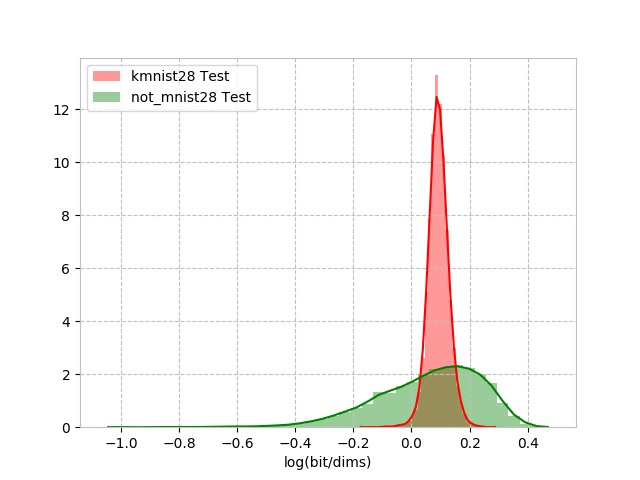
\includegraphics[width=0.5\columnwidth]{figures/kl_histogram-1}
\caption{Counter example of $LLR(x)$ with AUROC 0.1054 and 0.5143}
\end{figure}

\begin{figure}[H]
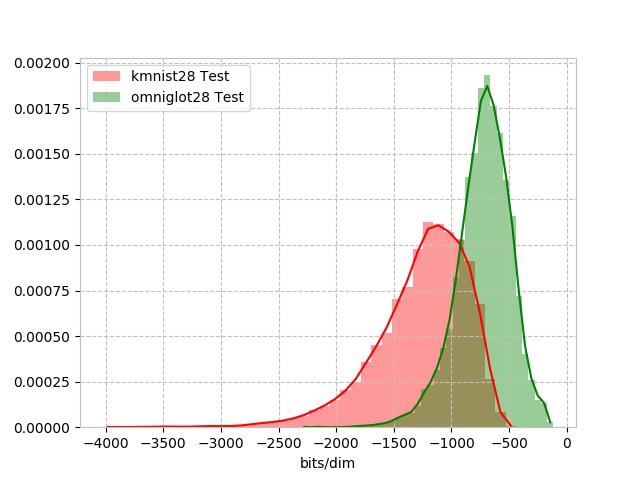
\includegraphics[width=0.5\columnwidth]{figures/ll_waic_histogram}
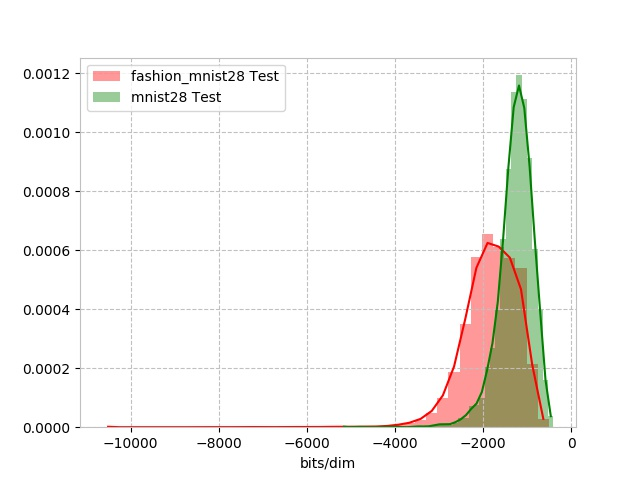
\includegraphics[width=0.5\columnwidth]{figures/ll_waic_histogram-1}
\caption{Counter example of $WAIC(x)$ with AUROC 0.1041 and 0.2135}
\end{figure}

\begin{figure}[H]
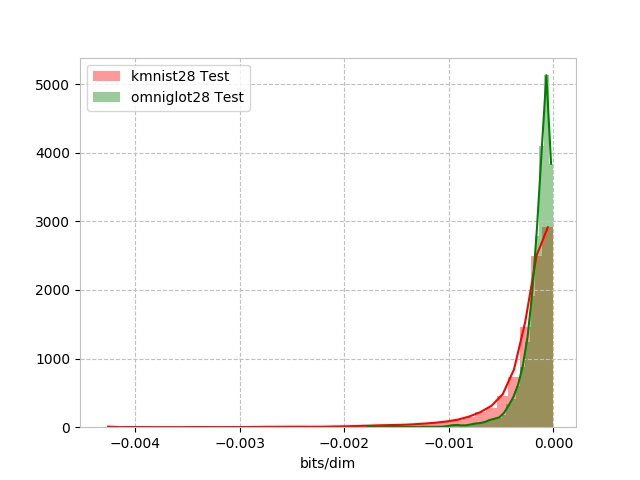
\includegraphics[width=0.5\columnwidth]{figures/var_log_prob_histogram}
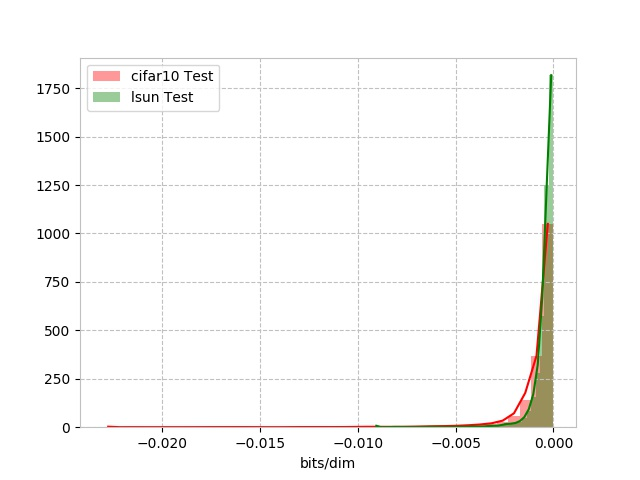
\includegraphics[width=0.5\columnwidth]{figures/var_log_prob_histogram-1}
\caption{Counter example of $\mathop{VAR}_\theta \log p_\theta(x)$ with AUROC 0.5358 and 0.3756}
\end{figure}

\begin{figure}[H]
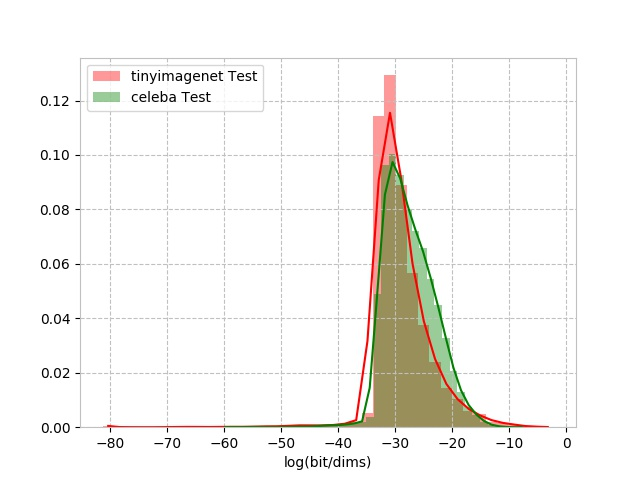
\includegraphics[width=0.5\columnwidth]{figures/log_prob_histogram-5}
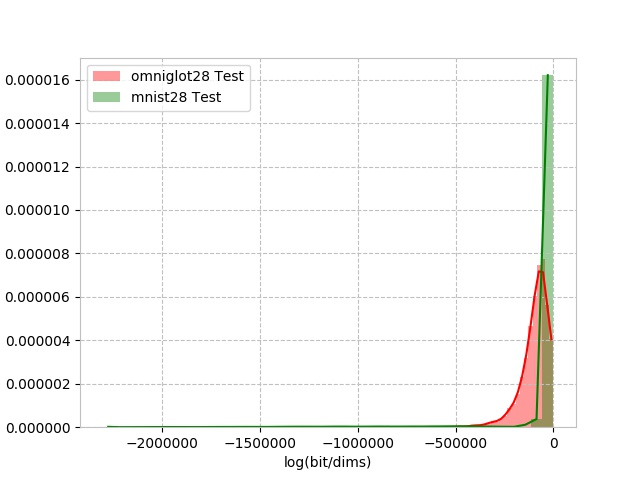
\includegraphics[width=0.5\columnwidth]{figures/log_prob_histogram-6}
\caption{Counter example of $\log p_\theta(x|y)$ with AUROC 0.3822 and 0.1150}
\end{figure}


\section{Appendix B Experiments}

The description of data is shown in the data appendix. 

The architecture of VAE is: 

\begin{table}[H]
\centering
\begin{tabular}{lllllll}
Layer     & Channel & Stride & Kernel & Activation  \\
\toprule
Resnet & 16 & 1x1 & 3x3 & Leaky ReLU \\
Resnet & 32 & 1x1 & 3x3 & Leaky ReLU \\
Resnet & 64 & 1x1 & 3x3 & Leaky ReLU \\
Resnet & 128 & 2x2 & 3x3 & Leaky ReLU \\
Resnet & 128 & 2x2 & 3x3 & Leaky ReLU \\
Resnet & 128 & 2x2 & 3x3 & Leaky ReLU \\
Flatten & \\
Dense & 256 &  &  & None \\
\bottomrule
\end{tabular}
\caption{Encoder architecture of VAE}
\end{table}

Before the decoder, we will use dense layer to map $z$ to a tensor with shape $8hw$ and reshape $(h / 4, w / 4, 128)$ where $h, w$ is the height and width of data. 

\begin{table}[H]
\centering
\begin{tabular}{lllllll}
Layer     & Channel & Stride & Kernel & Activation  \\
\toprule
Resnet Deconv & 128 & 2x2 & 3x3 & Leaky ReLU \\
Resnet Deconv & 128 & 2x2 & 3x3 & Leaky ReLU \\
Resnet Deconv & 128 & 2x2 & 3x3 & Leaky ReLU \\
Resnet Deconv & 64 & 1x1 & 3x3 & Leaky ReLU \\
Resnet Deconv & 32 & 1x1 & 3x3 & Leaky ReLU \\
Resnet Deconv & 16 & 1x1 & 3x3 & Leaky ReLU \\
Conv2d & 3 or 1 & 1x1 & 1x1 & None \\
\bottomrule
\end{tabular}
\caption{Decoder architecture of VAE}
\end{table}
We apply a Discretized Logistic Distribution as $p_\theta(x|z)$ and gaussian as $q_\phi(z|x)$. 


The architecture of PixelCNN is: 

\begin{table}[H]
\centering
\begin{tabular}{lllllll}
Layer     & Channel & Vertical Kernel & Horizontal Kernel& Activation & Dropout  \\
\toprule
Resnet & 64 & 2x3 & 2x2 & Leaky ReLU & 0.2\\
Resnet & 64 & 2x3 & 2x2 & Leaky ReLU & 0.2\\
Resnet & 64 & 2x3 & 2x2 & Leaky ReLU & 0.2\\
Resnet & 64 & 2x3 & 2x2 & Leaky ReLU & 0.2\\
Resnet & 64 & 2x3 & 2x2 & Leaky ReLU & 0.2\\
Resnet & 256 & 2x3 & 2x2 & Leaky ReLU & 0.2\\
Flatten & \\
Dense & 256 &  &  & None \\
\bottomrule
\end{tabular}
\caption{Architecture of PixelCNN}
\end{table}


The architecture of Wasserstein is: 

\begin{table}[H]
\centering
\begin{tabular}{lllllll}
Layer     & Channel & Stride & Kernel & Activation  \\
\toprule
Resnet Deconv & 128 & 2x2 & 3x3 & Leaky ReLU \\
Resnet Deconv & 128 & 2x2 & 3x3 & Leaky ReLU \\
Resnet Deconv & 128 & 1x1 & 3x3 & Leaky ReLU \\
Resnet Deconv & 64 & 1x1 & 3x3 & Leaky ReLU \\
Resnet Deconv & 32 & 1x1 & 3x3 & Leaky ReLU \\
Resnet Deconv & 16 & 1x1 & 3x3 & Leaky ReLU \\
Conv2d & 1 & 1x1 & 1x1 & None \\
\bottomrule
\end{tabular}
\caption{Generator architecture of WGAN}
\end{table}

\begin{table}[H]
\centering
\begin{tabular}{lllllll}
Layer     & Channel & Stride & Kernel & Activation  \\
\toprule
Resnet & 16 & 1x1 & 3x3 & Leaky ReLU \\
Resnet & 32 & 1x1 & 3x3 & Leaky ReLU \\
Resnet & 64 & 1x1 & 3x3 & Leaky ReLU \\
Resnet & 128 & 1x1 & 3x3 & Leaky ReLU \\
Resnet & 128 & 2x2 & 3x3 & Leaky ReLU \\
Resnet & 128 & 2x2 & 3x3 & Leaky ReLU \\
\bottomrule
\end{tabular}
\caption{Discriminator architecture of WGAN}
\end{table}

RealNVP has 3 level and 6 blocks at each level. Channel is 128 and activation is ReLU in each block. 

The hyper-parameters for VAE, PixelCNN, WGAN and Glow are shown in the scripts, shown in code appendix. 

The detailed experiments are shown in appendix D. 

The average runtime memory of VAE, PixelCNN, WGAN and Glow are 2.949GB, 2.851GB, 2.826GB and 2.917GB. 

\section{Appendix C Proofs}

We will derive the theorems in our papers by the assumptions:

\noindent \textbf{1.} The training data and testing data of in-distribution and out-of-distribution are i.i.d. .

\noindent \textbf{2.}  $div$ is a divergence , satisfying that $div(\pin, \pout) \gg 0$ and $div(\pout, \pin) \gg 0$.

\noindent \textbf{3.}  If $div(\pin, \pout)$ and $div(\pout, \pin)$ can be represented by sampling formula, \IE $div(\pin, \pout) \approx \sum_{i} f(x_i)$, then $f(x_i) \gg 0$ for almost $x_i$ in $\pin$.

\noindent \textbf{4.} $f: \mathcal{X} \rightarrow \mathcal{R}$ maps the distribution $\pin, \pout$ into two Gaussian distribution with constant variance.

\noindent \textbf{5.} Assumption 3 and 4 hold for any $\hat{f}$ approximating $f$.

\begin{lemma}\label{lemma1}
	Indicators $f_0$ and $f_1$ satisfying that if $f_0(x_1) < f_0(x_2)$ then $f_1(x_1) < f_1(x_2)$ and if $f_0(x_1) > f_0(x_2)$ then $f_1(x_1) > f_1(x_2)$ for $x_1, x_2$ in mixture distriution, have same performance for OoD. We call $f_0 \triangleq f_1$. 
\end{lemma}

\begin{proof}\rm
	Assume we get data $x_0, x_1, \ldots, x_n$ from mixture distribution. The metrics AUROC, AUPR, FPR@TPR95 and AP for indicator $f$ are all dependent on the order of $f(x_0), f(x_1), \ldots, f(x_n)$. The array $f_0(x_0), f_0(x_1), \ldots, f_0(x_n)$ and $f_1(x_0), f_1(x_1), \ldots, f_1(x_n)$ have the same order and then they have same performance for all metrics considered in OoD. \QED
\end{proof}

\begin{theorem}
	\label{thm1}
	$\log \pin(x) - \log \pout(x)$ is a symmetric indicator with great performance, \IE it reaches same performance in experiment A vs B and B vs A, with threshold zero.
\end{theorem}

\begin{proof}\rm
	We select $KL$ as $div$. By assumption 4, we have
	\begin{equation*}
		\log \pin(x_1) - \log \pout(x_1) \gg 0 \quad and \quad \log \pin(x_2) - \log \pout(x_2) \ll 0 
	\end{equation*}
	where $x_1 \sim \pin$ and $x_2 \sim \pout$. By assumption 5, above equation holds for $\log p_\theta(x) - \log p_\omega(x)$. Therefore, $\log \pin(x) - \log \pout(x)$ and $\log p_\theta(x) - \log p_\omega(x)$ can detect most of OoD, with threshold zero. 
	
	In experiment A vs B and B vs A, the indicator is $\log p_A(x) - \log p_B(x)$ and $\log p_B(x) - \log p_A(x)$. These two experiments have same mixture distribution. For any testing data $x_1, x_2$ in mixture distribution, if $\log p_A(x_1) - \log p_B(x_1) > \log p_A(x_2) - \log p_B(x_2)$, then $\log p_B(x_1) - \log p_A(x_1) < \log p_B(x_2) - \log p_A(x_2)$. Conversely, if $\log p_A(x_1) - \log p_B(x_1) < \log p_A(x_2) - \log p_B(x_2)$, then $\log p_B(x_1) - \log p_A(x_1) > \log p_B(x_2) - \log p_A(x_2)$. Thus, they have inverse order. 
	Noting that the positive and negative labels in experiment A vs B and B vs A are also inverse, $\log \pin(x) - \log \pout(x)$ reaches same performance in experiment A vs B and B vs A. \QED
\end{proof}

\begin{theorem}\label{thm2}
	For any mixture distribution $\pmix = \alpha \pin + \beta \pout$ where $\alpha + \beta = 1$ and $\alpha, \beta > 0$, the performance of indicator $\log \pin(x) - \log \pmix(x)$ and indicator $\log \pin(x) - \log \pout(x)$ is equal for OoD detection. 
\end{theorem}

\begin{proof}\rm
	For any $x1,x2$ satisfying $\log \pin(x_1) - \log \pout(x_1) < \log \pin(x_2) - \log \pout(x_2)$, we have $\log \pin(x_1) - \log \pmix(x_1) < \log \pin(x_2) - \log \pmix(x_2)$ by
	\begin{align*}
		&\log \pin(x) - \log \pmix(x) = -\log \frac{\alpha \pin(x) + \beta \pout(x)}{\pin(x)} = -\log 
		\Big(\alpha + \beta \frac{\pout(x)}{\pin(x)}\Big) \\
		&\log \frac{\pin(x_1)}{\pout(x_1)} < \log \frac{\pin(x_2)}{\pout(x_2)} \Rightarrow \frac{\pin(x_1)}{\pout(x_1)} < \frac{\pin(x_2)}{\pout(x_2)} \Rightarrow \frac{\pout(x_1)}{\pin(x_1)} > \frac{\pout(x_2)}{\pin(x_2)} \\
	 &\Rightarrow \log \Big(\alpha + \beta \frac{\pout(x_1)}{\pin(x_1)}\Big) > \log 
		\Big(\alpha + \beta \frac{\pout(x_2)}{\pin(x_2)}\Big) \\
		&\Rightarrow -(\log \pin(x_1) - \log \pmix(x_1)) > -(\log \pin(x_2) - \log \pmix(x_2)) \\
		&\Rightarrow \log \frac{\pin(x_1)}{\pmix(x_1)} < \log \frac{\pin(x_2)}{\pmix(x_2)} 
	\end{align*}
	
	By the same way, for any $x1,x2$ satisfying $\log \pin(x_1) - \log \pout(x_1) > \log \pin(x_2) - \log \pout(x_2)$, we have $\log \pin(x_1) - \log \pmix(x_1) > \log \pin(x_2) - \log \pmix(x_2)$.  By \cref{lemma1}, performance of indicator $\log \pin(x) - \log \pmix(x)$ and indicator $\log \pin(x) - \log \pout(x)$ is equal for OoD detection.
	
	\noindent \textbf{Remark.} In the proof, we do not use the condition that $\alpha > 0$ but only $\beta > 0$ and $\pmix(x) > 0$. It means that \cref{thm1} holds when $\alpha < 0, \beta > 0$ and $\pmix(x) > 0$. 
\QED
\end{proof}

\begin{theorem}\label{thm3}
When log-likelihood can detect OoD, \IE $\log \pin(x_1) > \log \pin(x_2)$ for almost $x_1 \sim \pin$ and $x_2 \sim \pout$, KL-based indicator can be also used to detect OoD.
\end{theorem}
\begin{proof}\rm
	Assume $\log \pout(x_1) < \log \pout(x_2)$, then $\log \pin(x_1) - \log \pout(x_1) > \log \pin(x_2) - \log \pout(x_2)$.
	KL-based indicator will get better performance than log-likelihood indicator. 
	
	Assume $\log \pout(x_1) > \log \pout(x_2)$, then likelihood indicator will make mistake in experiment B vs A (if current experiment is A vs B). Meanwhile KL-based indicator can detect OoD in both A vs B and B vs A by \cref{thm1}.  
	
	It means KL-based indicator is always better than log-likelihood indicator. 
\end{proof}

For the proofing of following theorems, we need an additional mathmatical simplification: by assumption 4 and 5, the indicators for OoD maps the distribution $\pin, \pout$ into two Gaussian distribution with constant variance, therefore, the AUROC between these two Gaussian distribution is dependent on the difference of their mean, \IE $\E_{\pin(x)} f(x) - \E_{\pout(x)} f(x)$ is our simplified metric for mathematical inference. 

\begin{theorem}\label{thm4}
For any likelihood-ratio indicator $\log \pin(x) - \log g(x)$ where $g$ is a continuous differentiable probability distribution, KL-based indicator outperforms them.
\end{theorem}
\begin{proof}\rm
	Consider the following optimization with subsidiary conditions for searching the optimal $g$ for likelihood ratio:
	\begin{align*}
	\max_g \Big\{\E_{\pin(x)} \big[\log \pin(x) - \log g(x)\big] &- \E_{\pout(x)} \big[\log \pin(x) - \log g(x)\big]\Big\} \\
	\textbf{s.t.} KL(\pin, g) = L \text{ and } &\int g(x) \dd x = 1 
	\end{align*}
	where $L$ is a constraint to the optimization domain of $g$. It could be solved by Lagrange multiplier method introduced by calculus of variation~\cite{gelfand2000calculus}. 
	Let $\lambda, \psi > 0$ be Lagrange Multiplier for the two constraint. The Lagrange function is 
	\begin{align*}
		J[g] &= \E_{\pin(x)} \big[\log \pin(x) - \log g(x)\big] - \E_{\pout(x)} \big[\log \pin(x) - \log g(x)\big] \\
		&-\lambda KL(\pin, g) - \psi \int g(x) \dd x \\
		&= \int \pin(x) \log \pin(x) - \pin(x) \log g(x) - \pout(x) \log \pin(x) \\ 
		&+ \pout(x) \log g(x) - \lambda \pin(x) \log \frac{\pin(x)}{g} - \psi g(x) \dd x = \int F(g, x) \dd x
	\end{align*}
	By calculus of variation, the extremal point for $J[g]$ satisfies that $\delta J = 0$, which is equal to
	\begin{align*}
		\frac{\partial F(g, x)}{\partial g} = 0 \Rightarrow -\frac{\pin(x)}{g(x)} + \frac{\pout(x)}{g(x)} + \frac{\lambda \pin(x)}{g(x)} - \psi = 0 \\
		\Rightarrow g(x) = \frac{1}{\psi} ((\lambda - 1)\pin(x) + \pout(x))
	\end{align*}
	Considering the subsidiary condition $\int g(x) \dd x = 1$, we have
	\begin{equation*}
		\int g(x) \dd x = \frac{1}{\psi} \int (\lambda - 1) \pin(x) + \pout(x) \dd x = \frac{1}{\psi} ((\lambda - 1) + 1) = \frac{\lambda}{\psi} = 1
	\end{equation*}
	Therefore, $\lambda = \psi$ and $g^*(x) = \frac{\lambda - 1}{\lambda} \pin(x) + \frac{1}{\lambda} \pout(x)$ is the extremal point.
	By the remark of \cref{thm1}, $\log \pin(x) - \log g^*(x)$ gets same performance as $\log \pin(x) - \log \pout(x)$ in OoD detection. 
	For any $L$, we can get $g^*(x)$, which has same performance as $\log \pin(x) - \log \pout(x)$. It means that KL-based indicator is the optimal indicator among all likelihood-ratio indicators. 
\end{proof}


\begin{theorem}\label{thm5}
	$\log \frac{p_\theta(x)}{p_\gamma(x)}$ can be used for detecting OoD. Moreover, $\log \frac{p_\theta(x)}{p_\gamma(x)}$ represents whether a sample $x$ in mixture distribution have been optimized in the training process of $\theta$.
\end{theorem}
\begin{proof}
	Let $p_{\hat{\gamma}}(x) = \alpha p_\theta(x) + \beta p_\omega(x)$. $\hat{\gamma}$ is the parameters that can be obtained by optimizer. 
	Considering the indicator $\log p_\theta(x) - \log p_{\hat{\gamma}}(x) = -\log (\alpha + \beta \frac{p_\omega(x)}{p_\theta(x)})$, for $x_1 \sim \pin$ and $x_2 \sim \pout$, we have 
	\begin{align*}
		\log \frac{p_\theta(x_1)}{p_{\hat{\gamma}}(x_1)} - \log \frac{p_\theta(x_2)}{p_{\hat{\gamma}}(x_2)} = \log (\alpha + \beta \frac{p_\omega(x_2)}{p_\theta(x_2)}) - \log (\alpha + \beta \frac{p_\omega(x_1)}{p_\theta(x_1)})
	\end{align*}
	We have known that $\log \frac{p_\theta(x_1)}{p_\omega(x_1)} \gg 0$ and $\log \frac{p_\theta(x_2)}{p_\omega(x_2)} \ll 0$ by \cref{thm1}. Then, we have $\log \frac{p_\theta(x_1)}{p_{\hat{\gamma}}(x_1)} - \log \frac{p_\theta(x_2)}{p_{\hat{\gamma}}(x_2)} > 0$. It means that $\log \frac{p_\theta(x)}{p_{\hat{\gamma}}(x)}$ can be used for detecting OoD.
	
	Next, consider the $\gamma$ is optimized better than $\hat{\gamma}$, \IE $\E_{\pmix} \log p_\gamma(x) \geq \E_{\pmix} \log p_{\hat{\gamma}}(x)$. 
	
	\begin{align*}
		\E_{\pmix} \log p_\gamma(x) = \alpha \E_{\pin} \log p_\gamma(x) + \beta \E_{\pout} \log p_\gamma(x)
	\end{align*}
	By $\E_{\pmix} \log p_\gamma(x) \geq \E_{\pmix} \log p_{\hat{\gamma}}(x)$, there are 3 case:
	
	\textbf{1.} $\E_{\pin} \log p_\gamma(x) \leq \E_{\pin} \log p_{\hat\gamma}(x)$ and $\E_{\pout} \log p_\gamma(x) \geq \E_{\pout} \log p_{\hat\gamma}(x)$. 
	
	\textbf{2.} $\E_{\pin} \log p_\gamma(x) \geq \E_{\pin} \log p_{\hat\gamma}(x)$ and $\E_{\pout} \log p_\gamma(x) \geq \E_{\pout} \log p_{\hat\gamma}(x)$. 
	
	
	\textbf{3.} $\E_{\pin} \log p_\gamma(x) \geq \E_{\pin} \log p_{\hat\gamma}(x)$ and $\E_{\pout} \log p_\gamma(x) \leq \E_{\pout} \log p_{\hat\gamma}(x)$. 
	
	By assumption 4, 5 and simplified metric, we know that if  $\E_{\pin} \log p_\gamma(x)$ increase, the KL-based indicator $\log \frac{p_\theta(x)}{p_{{\gamma}}(x)}$ will be worse and if  $\E_{\pout} \log p_\gamma(x)$ increase, the KL-based indicator $\log \frac{p_\theta(x)}{p_{{\gamma}}(x)}$ will be better. 
	
	Therefore, in case 1, the performance of $\log \frac{p_\theta(x_1)}{p_{\gamma}(x_1)}$ will be better than $\log \frac{p_\theta(x_1)}{p_{\hat\gamma}(x_1)}$. In case 2 and 3, we know $\E_{\pin} \log p_{\hat\gamma}(x) \leq \E_{\pin} \log p_\theta(x)$ and $\E_{\pin} \log p_\gamma(x) \leq \E_{\pin} \log p_\theta(x)$ since $\theta$ is well-trained for such loss function. 
	\begin{align*}
		\beta \E_{\pout} \log p_\gamma(x) = \E_{\pmix} \log p_\gamma(x) - \alpha \E_{\pin} \log p_\gamma(x) \\
		\geq \E_{\pmix} \log p_{\hat\gamma}(x) - \alpha \E_{\pin} \log p_\theta(x) \\
		= \alpha \E_{\pin} \log \frac{p_{\hat \gamma}(x)}{p_\theta(x)} + \beta \E_{\pout} \log p_{\hat \gamma}(x) \\
	\Rightarrow \E_{\pout} \log \frac{p_\gamma(x)}{p_{\hat\gamma}(x)} \geq \frac{\alpha}{\beta} \E_{\pin} \log \frac{p_{\hat \gamma}(x)}{p_\theta(x)}
	\end{align*}
	And we have 
	\begin{equation*}
		\E_{\pin} \log \frac{p_\gamma(x)}{p_{\hat\gamma}(x)} \leq \E_{\pin} \log \frac{p_\theta(x)}{p_{\hat\gamma}(x)}
	\end{equation*}
	Therefore, by our simplified metric, we have
	\begin{align*}
		(\E_{\pin(x)} \log \frac{p_\theta(x)}{p_{{\gamma}}(x)} - \E_{\pout(x)} \log \frac{p_\theta(x)}{p_{{\gamma}}(x)}) - (\E_{\pin(x)} \log \frac{p_\theta(x)}{p_{{\hat\gamma}}(x)} - \E_{\pout(x)} \log \frac{p_\theta(x)}{p_{\hat\gamma}(x)}) \\
		=  \E_{\pout} \log \frac{p_\gamma(x)}{p_{\hat\gamma}(x)} -\E_{\pin} \log \frac{p_{\gamma}(x)}{p_{\hat\gamma}(x)}\geq \frac{\alpha}{\beta} \E_{\pin} \log \frac{p_{\hat \gamma}(x)}{p_\theta(x)} - \E_{\pin} \log \frac{p_\theta(x)}{p_{\hat\gamma}(x)} \\
		= \frac{\alpha + \beta}{\beta} \E_{\pin} \log \frac{p_\theta(x)}{p_{\hat\gamma}(x)} = \frac{1}{\beta} \E_{\pin} \log \frac{p_\theta(x)}{p_{\hat\gamma}(x)} \geq 0
	\end{align*}
	It means that $\frac{p_\theta(x)}{p_{{\gamma}}(x)}$ is a better indicator than $\frac{p_\theta(x)}{p_{{\hat\gamma}}(x)}$ in cast 2 and 3. In conclusion,  $\frac{p_\theta(x)}{p_{{\gamma}}(x)}$ will be better and thus they can be used to detect OoD if $\gamma$ is trained better than $\hat{\gamma}$. 
	Additional, by the above proof, the most important property is that $\theta$ is well-trained in $\pin$ and thus $p_\gamma(x) < p_\theta(x)$ in $\pin$, \IE $\log \frac{p_\theta(x)}{p_\gamma(x)}$ represents whether a sample $x$ in mixture distribution have been optimized in the training process of $\theta$. 
\end{proof}

\begin{theorem}\label{thm6}
	Assumption 2 is a corollary of definition of OoD problem when $div$ is Wasserstein distance.
\end{theorem}
\begin{proof}
	By the definition of OoD, exist a $L > 0$, for any $x_1 \sim \pin, x_2 \sim \pout$, their distance $\|x_1 - x_2\|$ is at least $L$. 
	\begin{equation*}
		 W^1(\pin, \pout) = \min_{f \in \Gamma(\pin, \pout)} \iint f(x_1, x_2) \|x_1 - x_2\| \dd x_1 \dd x_2 \geq L
	\end{equation*}
\end{proof}

\begin{theorem}\label{thm7}
	$D(x)$ is a symmetric indicator.
\end{theorem}
\begin{proof}
	Let $D$ is the optimal discriminator in $W^1(\pin, \pout)$, for any $D'$ satisfying $Lip(D') \leq 1$, we have
	\begin{align*}
		\E_{\pout} D'(x) - \E_{\pin} D'(x) = \E_{\pin} [-D'(x)] - \E_{\pout} [-D'(x)] \\
		\leq  \E_{\pin} D(x) - \E_{\pout} D(x) =  \E_{\pout} [-D(x)] - \E_{\pin} [-D(x)] 
	\end{align*}
	Therefore, $-D(x)$ is the optimal discriminator in $W^1(\pout, \pin)$. By the same way in \cref{thm1}, 
	$D(x)$ is a symmetric indicator.
\end{proof}

\begin{theorem}\label{thm8}
	$\hat{D}$ that is optimal solution in $W^1(\pin, \pmix)$ is same to the optimal solution $D$ in $W^1(\pin, \pout)$. Moreover, the neural networks trained by $W^1(\pin, \pmix)$ and $W^1(\pin, \pout)$ will share the same optimization process.
\end{theorem}

\begin{proof}
	For any $D$ satisfying $Lip(D) \leq 1$, 
	\begin{align*}
		\E_{\pin} D(x) - \E_{\pmix} D(x) = \E_{\pin} D(x) - \alpha\E_{\pin} D(x) - \beta\E_{\pout} D(x) \\ 
		= (1 - \alpha)\E_{\pin} D(x) - \beta\E_{\pout} D(x)
		= \beta \E_{\pin} D(x) - \beta \E_{\pout} D(x) \\
		\leq \beta \E_{\pin} \hat{D}(x) - \beta \E_{\pout} \hat{D}(x) = (1 - \alpha)\E_{\pin} \hat{D}(x) - \beta\E_{\pout} \hat{D}(x) \\
		= \E_{\pin} \hat{D}(x) - \alpha\E_{\pin} \hat{D}(x) - \beta\E_{\pout} \hat{D}(x) = \E_{\pin} \hat{D}(x) - \E_{\pmix} \hat{D}(x)
	\end{align*}
	Therefore, $\hat{D}$ is also the optimal discriminator in $W^1(\pin, \pmix)$. Additional, in above proof, the loss functions for $D$ in $W^1(\pin, \pmix)$ and $W^1(\pin, \pout)$ are 
	\begin{equation*}
		\E_{\pin} D(x) - \E_{\pmix} D(x) = \beta (\E_{\pin} D(x) - \E_{\pout} D(x))
	\end{equation*}
	The two loss functions have same gradient direction for neural network optimization, thus the training optimization processes are same.
\end{proof}

\begin{theorem}\label{thm9}
	The discriminator in $W^1(\pin, \pout)$ is the best indicator among all indicators that is 1-Lipschitz. Moreover, it is the best indicator who has limited gradient.
\end{theorem}
\begin{proof}
	By our simplified metric, for any indicator $f$, 
	\begin{equation*}
		\E_{\pin} f(x) - \E_{\pout} f(x)
	\end{equation*}
	measures the performance of OoD detection. Thus 
	\begin{equation*}
		\max_{Lip(f) \leq 1} \E_{\pin} f(x) - \E_{\pout} f(x) = W^1(\pin, \pout)
	\end{equation*} 
	will search the best indicator among all indicators that is 1-Lipschitz. Especially, for a indicator $f$ has limited gradient $K$, function $g(x) = f(x) / K$ satisfies that $Lip(g) \leq 1$. By \cref{thm1}, $f \triangleq g$, and $g$ is worse than the optimal discriminator in $W^1(\pin, \pout)$. 
	
\end{proof}

\section{Appendix D Detailed Experiments}




\clearpage
\begin{longtable}{lrrrrr}
Dataset pair & AUROC & AUPR & AP & FPR@TPR95 \\
\toprule
CIFAR-10 vs CelebA & 0.2625 & 0.2552 & 0.2552 & 0.9988 \\
CIFAR-10 vs Constant & 0.0000 & 0.3069 & 0.3069 & 1.0000 \\
CIFAR-10 vs LSUN & 0.8077 & 0.7755 & 0.7756 & 0.5685 \\
CIFAR-10 vs Noise & 0.8120 & 0.8979 & 0.8979 & 1.0000 \\
CIFAR-10 vs SVHN & 0.0113 & 0.1541 & 0.1541 & 0.9999 \\
CIFAR-10 vs iSUN & 0.7914 & 0.7683 & 0.7684 & 0.5545 \\
CIFAR-100 vs CelebA & 0.2912 & 0.2874 & 0.2875 & 0.9992 \\
CIFAR-100 vs Constant & 0.0000 & 0.3069 & 0.3069 & 1.0000 \\
CIFAR-100 vs LSUN & 0.7933 & 0.7808 & 0.7808 & 0.6609 \\
CIFAR-100 vs Noise & 0.7571 & 0.8667 & 0.8667 & 1.0000 \\
CIFAR-100 vs SVHN & 0.0157 & 0.1541 & 0.1542 & 1.0000 \\
CIFAR-100 vs iSUN & 0.7751 & 0.7688 & 0.7688 & 0.6319 \\
CelebA vs CIFAR-10 & 0.3563 & 0.5538 & 0.5538 & 0.9445 \\
CelebA vs CIFAR-100 & 0.3943 & 0.5673 & 0.5674 & 0.9100 \\
CelebA vs Constant & 0.0000 & 0.4503 & 0.4503 & 1.0000 \\
CelebA vs LSUN & 0.7582 & 0.8007 & 0.8007 & 0.5615 \\
CelebA vs Noise & 0.5293 & 0.8071 & 0.8071 & 1.0000 \\
CelebA vs SVHN & 0.0012 & 0.2578 & 0.2578 & 0.9999 \\
CelebA vs TinyImagenet & 0.4525 & 0.6027 & 0.6027 & 0.8843 \\
CelebA vs iSUN & 0.7204 & 0.7773 & 0.7774 & 0.5683 \\
Constant vs CIFAR-10 & 0.8342 & 0.8686 & 0.8686 & 0.9233 \\
Constant vs CIFAR-100 & 0.9044 & 0.8981 & 0.8981 & 0.4665 \\
Constant vs CelebA & 0.8776 & 0.8748 & 0.8748 & 0.8937 \\
Constant vs LSUN & 0.8262 & 0.8610 & 0.8610 & 0.8622 \\
Constant vs Noise & 0.5041 & 0.7094 & 0.7094 & 1.0000 \\
Constant vs SVHN & 0.4682 & 0.3954 & 0.3955 & 0.9986 \\
Constant vs TinyImagenet & 0.9766 & 0.9758 & 0.9758 & 0.1035 \\
Constant vs iSUN & 0.8959 & 0.9220 & 0.9220 & 0.6016 \\
Constant28 vs FashionMNIST & 0.0053 & 0.3119 & 0.3119 & 1.0000 \\
Constant28 vs KMNIST & 0.0080 & 0.3148 & 0.3148 & 1.0000 \\
Constant28 vs MNIST & 0.0050 & 0.3118 & 0.3119 & 1.0000 \\
Constant28 vs Noise28 & 0.5475 & 0.7395 & 0.7395 & 1.0000 \\
Constant28 vs NotMNIST & 0.0125 & 0.3097 & 0.3097 & 0.9976 \\
Constant28 vs Omniglot & 0.0050 & 0.3545 & 0.3545 & 1.0000 \\
FashionMNIST vs Constant28 & 0.0000 & 0.3069 & 0.3069 & 1.0000 \\
FashionMNIST vs KMNIST & 0.0830 & 0.3154 & 0.3155 & 1.0000 \\
FashionMNIST vs MNIST & 0.0000 & 0.3069 & 0.3069 & 1.0000 \\
FashionMNIST vs Noise28 & 1.0000 & 1.0000 & 1.0000 & 0.0000 \\
FashionMNIST vs NotMNIST & 0.0608 & 0.3138 & 0.3138 & 0.9968 \\
FashionMNIST vs Omniglot & 0.0005 & 0.3495 & 0.3495 & 1.0000 \\
KMNIST vs Constant28 & 0.0000 & 0.3069 & 0.3069 & 1.0000 \\
KMNIST vs FashionMNIST & 0.5176 & 0.4956 & 0.4957 & 0.9359 \\
KMNIST vs MNIST & 0.0005 & 0.3069 & 0.3069 & 1.0000 \\
KMNIST vs Noise28 & 1.0000 & 1.0000 & 1.0000 & 0.0000 \\
KMNIST vs NotMNIST & 0.2176 & 0.3472 & 0.3472 & 0.9714 \\
KMNIST vs Omniglot & 0.0186 & 0.3509 & 0.3509 & 1.0000 \\
MNIST vs Constant28 & 0.0000 & 0.3069 & 0.3069 & 1.0000 \\
MNIST vs FashionMNIST & 0.9179 & 0.8975 & 0.8975 & 0.2460 \\
MNIST vs KMNIST & 0.8494 & 0.8367 & 0.8367 & 0.4494 \\
MNIST vs Noise28 & 1.0000 & 1.0000 & 1.0000 & 0.0000 \\
MNIST vs NotMNIST & 0.7736 & 0.7060 & 0.7060 & 0.5816 \\
MNIST vs Omniglot & 0.1968 & 0.3886 & 0.3887 & 0.9892 \\
Noise vs CIFAR-10 & 0.0019 & 0.3072 & 0.3072 & 0.9983 \\
Noise vs CIFAR-100 & 0.0000 & 0.3069 & 0.3069 & 1.0000 \\
Noise vs CelebA & 0.0000 & 0.1893 & 0.1894 & 1.0000 \\
Noise vs Constant & 0.4954 & 0.4479 & 0.4479 & 0.5261 \\
Noise vs LSUN & 0.0000 & 0.3069 & 0.3069 & 1.0000 \\
Noise vs SVHN & 0.0000 & 0.1537 & 0.1538 & 1.0000 \\
Noise vs TinyImagenet & 0.0000 & 0.3105 & 0.3106 & 1.0000 \\
Noise vs iSUN & 0.0000 & 0.3292 & 0.3292 & 1.0000 \\
Noise28 vs Constant28 & 0.0000 & 0.3069 & 0.3069 & 1.0000 \\
Noise28 vs FashionMNIST & 0.0000 & 0.3069 & 0.3069 & 1.0000 \\
Noise28 vs KMNIST & 0.0000 & 0.3069 & 0.3069 & 1.0000 \\
Noise28 vs MNIST & 0.0000 & 0.3069 & 0.3069 & 1.0000 \\
Noise28 vs NotMNIST & 0.0000 & 0.3069 & 0.3069 & 1.0000 \\
Noise28 vs Omniglot & 0.0000 & 0.3495 & 0.3495 & 1.0000 \\
NotMNIST vs Constant28 & 0.0025 & 0.3069 & 0.3069 & 1.0000 \\
NotMNIST vs FashionMNIST & 0.2368 & 0.3527 & 0.3528 & 0.9888 \\
NotMNIST vs KMNIST & 0.1037 & 0.3321 & 0.3322 & 0.9995 \\
NotMNIST vs MNIST & 0.0000 & 0.3069 & 0.3069 & 1.0000 \\
NotMNIST vs Noise28 & 1.0000 & 1.0000 & 1.0000 & 0.0000 \\
NotMNIST vs Omniglot & 0.0000 & 0.3495 & 0.3495 & 1.0000 \\
Omniglot vs Constant28 & 0.0002 & 0.2668 & 0.2669 & 1.0000 \\
Omniglot vs FashionMNIST & 0.9403 & 0.9222 & 0.9222 & 0.2575 \\
Omniglot vs KMNIST & 0.9139 & 0.9018 & 0.9018 & 0.3882 \\
Omniglot vs MNIST & 0.3969 & 0.4195 & 0.4196 & 1.0000 \\
Omniglot vs Noise28 & 1.0000 & 1.0000 & 1.0000 & 0.0000 \\
Omniglot vs NotMNIST & 0.6918 & 0.6052 & 0.6053 & 0.8355 \\
SVHN vs CIFAR-10 & 0.9251 & 0.9547 & 0.9548 & 0.2770 \\
SVHN vs CIFAR-100 & 0.9158 & 0.9438 & 0.9438 & 0.2859 \\
SVHN vs CelebA & 0.8934 & 0.9259 & 0.9259 & 0.5886 \\
SVHN vs Constant & 0.0000 & 0.5076 & 0.5076 & 1.0000 \\
SVHN vs LSUN & 0.9884 & 0.9951 & 0.9951 & 0.0545 \\
SVHN vs Noise & 0.7951 & 0.9378 & 0.9378 & 1.0000 \\
SVHN vs TinyImagenet & 0.9453 & 0.9702 & 0.9702 & 0.2248 \\
SVHN vs iSUN & 0.9840 & 0.9938 & 0.9938 & 0.0801 \\
TinyImagenet vs CelebA & 0.2307 & 0.2425 & 0.2425 & 0.9996 \\
TinyImagenet vs Constant & 0.0000 & 0.3032 & 0.3032 & 1.0000 \\
TinyImagenet vs LSUN & 0.7219 & 0.6950 & 0.6950 & 0.7544 \\
TinyImagenet vs Noise & 0.7274 & 0.8476 & 0.8476 & 1.0000 \\
TinyImagenet vs SVHN & 0.0086 & 0.1515 & 0.1516 & 1.0000 \\
TinyImagenet vs iSUN & 0.7151 & 0.6958 & 0.6959 & 0.7091 \\
Average  & 0.3986 & 0.5509 & 0.5510 & 0.7964 \\
\bottomrule
\caption{The detailed performance for indicator $\log p_\omega(x)$ based on model VAE }
% models/likelihood/vae.py --use_transductive=False --count_experiment=True log_prob_mixed
\label{tab0}
\end{longtable}


\clearpage
\begin{longtable}{lrrrrr}
Dataset pair & AUROC & AUPR & AP & FPR@TPR95 \\
\toprule
CIFAR-10 vs CelebA & 0.9969 & 0.9962 & 0.9962 & 0.0021 \\
CIFAR-10 vs Constant & 1.0000 & 1.0000 & 1.0000 & 0.0000 \\
CIFAR-10 vs LSUN & 0.9985 & 0.9990 & 0.9990 & 0.0003 \\
CIFAR-10 vs Noise & 1.0000 & 1.0000 & 1.0000 & 0.0000 \\
CIFAR-10 vs SVHN & 0.9994 & 0.9984 & 0.9984 & 0.0013 \\
CIFAR-10 vs iSUN & 0.9979 & 0.9980 & 0.9980 & 0.0019 \\
CIFAR-100 vs CelebA & 0.9984 & 0.9974 & 0.9974 & 0.0029 \\
CIFAR-100 vs Constant & 1.0000 & 1.0000 & 1.0000 & 0.0000 \\
CIFAR-100 vs LSUN & 0.9988 & 0.9980 & 0.9980 & 0.0038 \\
CIFAR-100 vs Noise & 1.0000 & 1.0000 & 1.0000 & 0.0000 \\
CIFAR-100 vs SVHN & 0.9993 & 0.9978 & 0.9978 & 0.0023 \\
CIFAR-100 vs iSUN & 0.9996 & 0.9994 & 0.9994 & 0.0013 \\
CelebA vs CIFAR-10 & 0.9976 & 0.9970 & 0.9970 & 0.0051 \\
CelebA vs CIFAR-100 & 0.9991 & 0.9996 & 0.9996 & 0.0023 \\
CelebA vs Constant & 1.0000 & 1.0000 & 1.0000 & 0.0000 \\
CelebA vs LSUN & 1.0000 & 1.0000 & 1.0000 & 0.0000 \\
CelebA vs Noise & 1.0000 & 1.0000 & 1.0000 & 0.0000 \\
CelebA vs SVHN & 1.0000 & 1.0000 & 1.0000 & 0.0000 \\
CelebA vs TinyImagenet & 0.9992 & 0.9997 & 0.9997 & 0.0002 \\
CelebA vs iSUN & 0.9999 & 1.0000 & 1.0000 & 0.0001 \\
Constant vs CIFAR-10 & 1.0000 & 1.0000 & 1.0000 & 0.0000 \\
Constant vs CIFAR-100 & 1.0000 & 1.0000 & 1.0000 & 0.0000 \\
Constant vs CelebA & 1.0000 & 1.0000 & 1.0000 & 0.0000 \\
Constant vs LSUN & 1.0000 & 1.0000 & 1.0000 & 0.0000 \\
Constant vs Noise & 1.0000 & 1.0000 & 1.0000 & 0.0000 \\
Constant vs SVHN & 1.0000 & 1.0000 & 1.0000 & 0.0000 \\
Constant vs TinyImagenet & 1.0000 & 1.0000 & 1.0000 & 0.0000 \\
Constant vs iSUN & 1.0000 & 1.0000 & 1.0000 & 0.0000 \\
Constant28 vs FashionMNIST & 1.0000 & 1.0000 & 1.0000 & 0.0000 \\
Constant28 vs KMNIST & 1.0000 & 1.0000 & 1.0000 & 0.0000 \\
Constant28 vs MNIST & 1.0000 & 1.0000 & 1.0000 & 0.0000 \\
Constant28 vs Noise28 & 1.0000 & 1.0000 & 1.0000 & 0.0000 \\
Constant28 vs NotMNIST & 1.0000 & 1.0000 & 1.0000 & 0.0000 \\
Constant28 vs Omniglot & 1.0000 & 1.0000 & 1.0000 & 0.0000 \\
FashionMNIST vs Constant28 & 1.0000 & 1.0000 & 1.0000 & 0.0000 \\
FashionMNIST vs KMNIST & 1.0000 & 1.0000 & 1.0000 & 0.0000 \\
FashionMNIST vs MNIST & 1.0000 & 1.0000 & 1.0000 & 0.0000 \\
FashionMNIST vs Noise28 & 1.0000 & 1.0000 & 1.0000 & 0.0000 \\
FashionMNIST vs NotMNIST & 1.0000 & 1.0000 & 1.0000 & 0.0001 \\
FashionMNIST vs Omniglot & 1.0000 & 1.0000 & 1.0000 & 0.0000 \\
KMNIST vs Constant28 & 1.0000 & 1.0000 & 1.0000 & 0.0000 \\
KMNIST vs FashionMNIST & 1.0000 & 1.0000 & 1.0000 & 0.0000 \\
KMNIST vs MNIST & 1.0000 & 1.0000 & 1.0000 & 0.0000 \\
KMNIST vs Noise28 & 1.0000 & 1.0000 & 1.0000 & 0.0000 \\
KMNIST vs NotMNIST & 1.0000 & 1.0000 & 1.0000 & 0.0000 \\
KMNIST vs Omniglot & 0.9999 & 0.9999 & 0.9999 & 0.0002 \\
MNIST vs Constant28 & 1.0000 & 1.0000 & 1.0000 & 0.0000 \\
MNIST vs FashionMNIST & 1.0000 & 1.0000 & 1.0000 & 0.0000 \\
MNIST vs KMNIST & 1.0000 & 1.0000 & 1.0000 & 0.0000 \\
MNIST vs Noise28 & 1.0000 & 1.0000 & 1.0000 & 0.0000 \\
MNIST vs NotMNIST & 1.0000 & 1.0000 & 1.0000 & 0.0000 \\
MNIST vs Omniglot & 1.0000 & 1.0000 & 1.0000 & 0.0000 \\
Noise vs CIFAR-10 & 0.9976 & 0.9867 & 0.9867 & 0.0028 \\
Noise vs CIFAR-100 & 1.0000 & 1.0000 & 1.0000 & 0.0000 \\
Noise vs CelebA & 1.0000 & 1.0000 & 1.0000 & 0.0000 \\
Noise vs Constant & 0.5333 & 0.4649 & 0.4652 & 0.4873 \\
Noise vs LSUN & 1.0000 & 1.0000 & 1.0000 & 0.0000 \\
Noise vs SVHN & 1.0000 & 1.0000 & 1.0000 & 0.0000 \\
Noise vs TinyImagenet & 1.0000 & 1.0000 & 1.0000 & 0.0000 \\
Noise vs iSUN & 1.0000 & 1.0000 & 1.0000 & 0.0000 \\
Noise28 vs Constant28 & 1.0000 & 1.0000 & 1.0000 & 0.0000 \\
Noise28 vs FashionMNIST & 1.0000 & 1.0000 & 1.0000 & 0.0000 \\
Noise28 vs KMNIST & 1.0000 & 1.0000 & 1.0000 & 0.0000 \\
Noise28 vs MNIST & 1.0000 & 1.0000 & 1.0000 & 0.0000 \\
Noise28 vs NotMNIST & 1.0000 & 1.0000 & 1.0000 & 0.0000 \\
Noise28 vs Omniglot & 1.0000 & 1.0000 & 1.0000 & 0.0000 \\
NotMNIST vs Constant28 & 0.9999 & 0.9999 & 0.9999 & 0.0000 \\
NotMNIST vs FashionMNIST & 1.0000 & 1.0000 & 1.0000 & 0.0000 \\
NotMNIST vs KMNIST & 1.0000 & 1.0000 & 1.0000 & 0.0000 \\
NotMNIST vs MNIST & 1.0000 & 1.0000 & 1.0000 & 0.0000 \\
NotMNIST vs Noise28 & 1.0000 & 1.0000 & 1.0000 & 0.0000 \\
NotMNIST vs Omniglot & 1.0000 & 1.0000 & 1.0000 & 0.0000 \\
Omniglot vs Constant28 & 1.0000 & 1.0000 & 1.0000 & 0.0000 \\
Omniglot vs FashionMNIST & 1.0000 & 1.0000 & 1.0000 & 0.0000 \\
Omniglot vs KMNIST & 1.0000 & 1.0000 & 1.0000 & 0.0000 \\
Omniglot vs MNIST & 1.0000 & 1.0000 & 1.0000 & 0.0000 \\
Omniglot vs Noise28 & 1.0000 & 1.0000 & 1.0000 & 0.0000 \\
Omniglot vs NotMNIST & 1.0000 & 1.0000 & 1.0000 & 0.0000 \\
SVHN vs CIFAR-10 & 0.9989 & 0.9996 & 0.9996 & 0.0002 \\
SVHN vs CIFAR-100 & 0.9986 & 0.9995 & 0.9995 & 0.0005 \\
SVHN vs CelebA & 1.0000 & 1.0000 & 1.0000 & 0.0000 \\
SVHN vs Constant & 1.0000 & 1.0000 & 1.0000 & 0.0000 \\
SVHN vs LSUN & 1.0000 & 1.0000 & 1.0000 & 0.0000 \\
SVHN vs Noise & 1.0000 & 1.0000 & 1.0000 & 0.0000 \\
SVHN vs TinyImagenet & 0.9985 & 0.9995 & 0.9995 & 0.0003 \\
SVHN vs iSUN & 1.0000 & 1.0000 & 1.0000 & 0.0000 \\
TinyImagenet vs CelebA & 0.9984 & 0.9955 & 0.9955 & 0.0057 \\
TinyImagenet vs Constant & 1.0000 & 1.0000 & 1.0000 & 0.0000 \\
TinyImagenet vs LSUN & 1.0000 & 1.0000 & 1.0000 & 0.0000 \\
TinyImagenet vs Noise & 1.0000 & 1.0000 & 1.0000 & 0.0000 \\
TinyImagenet vs SVHN & 0.9992 & 0.9976 & 0.9976 & 0.0019 \\
TinyImagenet vs iSUN & 0.9998 & 0.9998 & 0.9998 & 0.0001 \\
Average  & 0.9947 & 0.9937 & 0.9937 & 0.0057 \\
\bottomrule
\caption{The detailed performance for indicator $\log p_\theta(x) - \log p_\omega(x)$ based on model VAE }
% models/likelihood/vae.py --use_transductive=False --count_experiment=True kl
\label{tab0}
\end{longtable}



\clearpage
\begin{longtable}{lrrrrr}
Dataset pair & AUROC & AUPR & AP & FPR@TPR95 \\
\toprule
CIFAR-10 vs CelebA & 0.6911 & 0.6042 & 0.6042 & 0.9335 \\
CIFAR-10 vs Constant & 0.1272 & 0.3261 & 0.3262 & 0.9796 \\
CIFAR-10 vs LSUN & 0.9336 & 0.9182 & 0.9182 & 0.2429 \\
CIFAR-10 vs Noise & 1.0000 & 1.0000 & 1.0000 & 0.0000 \\
CIFAR-10 vs SVHN & 0.0813 & 0.1594 & 0.1594 & 0.9997 \\
CIFAR-10 vs iSUN & 0.9138 & 0.9004 & 0.9005 & 0.2882 \\
CIFAR-100 vs CelebA & 0.6420 & 0.5742 & 0.5742 & 0.9728 \\
CIFAR-100 vs Constant & 0.1104 & 0.3232 & 0.3232 & 0.9905 \\
CIFAR-100 vs LSUN & 0.9251 & 0.9140 & 0.9140 & 0.2849 \\
CIFAR-100 vs Noise & 1.0000 & 1.0000 & 1.0000 & 0.0000 \\
CIFAR-100 vs SVHN & 0.0891 & 0.1649 & 0.1649 & 1.0000 \\
CIFAR-100 vs iSUN & 0.9071 & 0.9015 & 0.9015 & 0.3280 \\
CelebA vs CIFAR-10 & 0.7455 & 0.7874 & 0.7874 & 0.6181 \\
CelebA vs CIFAR-100 & 0.7084 & 0.7474 & 0.7474 & 0.6327 \\
CelebA vs Constant & 0.1153 & 0.4741 & 0.4741 & 0.9499 \\
CelebA vs LSUN & 0.9762 & 0.9806 & 0.9806 & 0.0782 \\
CelebA vs Noise & 1.0000 & 1.0000 & 1.0000 & 0.0000 \\
CelebA vs SVHN & 0.1098 & 0.2713 & 0.2713 & 0.9954 \\
CelebA vs TinyImagenet & 0.7797 & 0.8134 & 0.8134 & 0.5426 \\
CelebA vs iSUN & 0.9707 & 0.9804 & 0.9804 & 0.0993 \\
Constant vs CIFAR-10 & 1.0000 & 1.0000 & 1.0000 & 0.0000 \\
Constant vs CIFAR-100 & 1.0000 & 1.0000 & 1.0000 & 0.0000 \\
Constant vs CelebA & 1.0000 & 1.0000 & 1.0000 & 0.0000 \\
Constant vs LSUN & 1.0000 & 1.0000 & 1.0000 & 0.0000 \\
Constant vs Noise & 1.0000 & 1.0000 & 1.0000 & 0.0000 \\
Constant vs SVHN & 1.0000 & 1.0000 & 1.0000 & 0.0000 \\
Constant vs TinyImagenet & 1.0000 & 1.0000 & 1.0000 & 0.0000 \\
Constant vs iSUN & 1.0000 & 1.0000 & 1.0000 & 0.0000 \\
Constant28 vs FashionMNIST & 1.0000 & 1.0000 & 1.0000 & 0.0000 \\
Constant28 vs KMNIST & 1.0000 & 1.0000 & 1.0000 & 0.0000 \\
Constant28 vs MNIST & 1.0000 & 1.0000 & 1.0000 & 0.0000 \\
Constant28 vs Noise28 & 1.0000 & 1.0000 & 1.0000 & 0.0000 \\
Constant28 vs NotMNIST & 0.9994 & 0.9994 & 0.9994 & 0.0032 \\
Constant28 vs Omniglot & 0.9996 & 0.9997 & 0.9997 & 0.0024 \\
FashionMNIST vs Constant28 & 0.9918 & 0.9666 & 0.9667 & 0.0080 \\
FashionMNIST vs KMNIST & 0.4843 & 0.5098 & 0.5099 & 0.9587 \\
FashionMNIST vs MNIST & 0.0968 & 0.3177 & 0.3177 & 1.0000 \\
FashionMNIST vs Noise28 & 1.0000 & 1.0000 & 1.0000 & 0.0000 \\
FashionMNIST vs NotMNIST & 0.8435 & 0.8373 & 0.8373 & 0.5505 \\
FashionMNIST vs Omniglot & 0.0609 & 0.3557 & 0.3557 & 1.0000 \\
KMNIST vs Constant28 & 0.9920 & 0.9613 & 0.9614 & 0.0080 \\
KMNIST vs FashionMNIST & 0.9197 & 0.9053 & 0.9053 & 0.3066 \\
KMNIST vs MNIST & 0.1667 & 0.3338 & 0.3339 & 1.0000 \\
KMNIST vs Noise28 & 1.0000 & 1.0000 & 1.0000 & 0.0000 \\
KMNIST vs NotMNIST & 0.9253 & 0.8799 & 0.8800 & 0.2867 \\
KMNIST vs Omniglot & 0.0905 & 0.3615 & 0.3615 & 1.0000 \\
MNIST vs Constant28 & 0.9950 & 0.9735 & 0.9735 & 0.0050 \\
MNIST vs FashionMNIST & 1.0000 & 1.0000 & 1.0000 & 0.0000 \\
MNIST vs KMNIST & 0.9995 & 0.9994 & 0.9994 & 0.0020 \\
MNIST vs Noise28 & 1.0000 & 1.0000 & 1.0000 & 0.0000 \\
MNIST vs NotMNIST & 1.0000 & 1.0000 & 1.0000 & 0.0000 \\
MNIST vs Omniglot & 0.5971 & 0.5853 & 0.5854 & 0.7052 \\
Noise vs CIFAR-10 & 0.1883 & 0.3474 & 0.3474 & 0.8324 \\
Noise vs CIFAR-100 & 0.2428 & 0.3616 & 0.3617 & 0.7782 \\
Noise vs CelebA & 0.4722 & 0.2944 & 0.2944 & 0.5673 \\
Noise vs Constant & 0.4959 & 0.4480 & 0.4481 & 0.5254 \\
Noise vs LSUN & 0.1123 & 0.3294 & 0.3294 & 0.9080 \\
Noise vs SVHN & 0.2078 & 0.1840 & 0.1840 & 0.8067 \\
Noise vs TinyImagenet & 0.2691 & 0.3728 & 0.3729 & 0.7564 \\
Noise vs iSUN & 0.0816 & 0.3457 & 0.3457 & 0.9332 \\
Noise28 vs Constant28 & 0.4525 & 0.4304 & 0.4304 & 0.5630 \\
Noise28 vs FashionMNIST & 0.0000 & 0.3069 & 0.3069 & 1.0000 \\
Noise28 vs KMNIST & 0.0000 & 0.3069 & 0.3069 & 1.0000 \\
Noise28 vs MNIST & 0.0000 & 0.3069 & 0.3069 & 1.0000 \\
Noise28 vs NotMNIST & 0.0000 & 0.3069 & 0.3069 & 1.0000 \\
Noise28 vs Omniglot & 0.0000 & 0.3495 & 0.3495 & 1.0000 \\
NotMNIST vs Constant28 & 0.9861 & 0.9623 & 0.9624 & 0.0080 \\
NotMNIST vs FashionMNIST & 0.9340 & 0.9370 & 0.9370 & 0.3698 \\
NotMNIST vs KMNIST & 0.7911 & 0.8013 & 0.8013 & 0.8417 \\
NotMNIST vs MNIST & 0.4329 & 0.4689 & 0.4689 & 1.0000 \\
NotMNIST vs Noise28 & 1.0000 & 1.0000 & 1.0000 & 0.0000 \\
NotMNIST vs Omniglot & 0.3232 & 0.4532 & 0.4532 & 0.9994 \\
Omniglot vs Constant28 & 0.9950 & 0.9685 & 0.9685 & 0.0050 \\
Omniglot vs FashionMNIST & 0.9993 & 0.9992 & 0.9992 & 0.0033 \\
Omniglot vs KMNIST & 0.9821 & 0.9795 & 0.9795 & 0.1071 \\
Omniglot vs MNIST & 0.8131 & 0.7697 & 0.7697 & 0.6612 \\
Omniglot vs Noise28 & 1.0000 & 1.0000 & 1.0000 & 0.0000 \\
Omniglot vs NotMNIST & 1.0000 & 1.0000 & 1.0000 & 0.0000 \\
SVHN vs CIFAR-10 & 0.9915 & 0.9961 & 0.9961 & 0.0375 \\
SVHN vs CIFAR-100 & 0.9878 & 0.9944 & 0.9944 & 0.0506 \\
SVHN vs CelebA & 0.9990 & 0.9993 & 0.9993 & 0.0011 \\
SVHN vs Constant & 0.6388 & 0.7412 & 0.7412 & 0.6615 \\
SVHN vs LSUN & 0.9997 & 0.9999 & 0.9999 & 0.0010 \\
SVHN vs Noise & 1.0000 & 1.0000 & 1.0000 & 0.0000 \\
SVHN vs TinyImagenet & 0.9931 & 0.9969 & 0.9969 & 0.0281 \\
SVHN vs iSUN & 0.9995 & 0.9998 & 0.9998 & 0.0015 \\
TinyImagenet vs CelebA & 0.5599 & 0.4693 & 0.4693 & 0.9853 \\
TinyImagenet vs Constant & 0.0639 & 0.3100 & 0.3100 & 0.9980 \\
TinyImagenet vs LSUN & 0.9095 & 0.8893 & 0.8894 & 0.3165 \\
TinyImagenet vs Noise & 1.0000 & 1.0000 & 1.0000 & 0.0000 \\
TinyImagenet vs SVHN & 0.0575 & 0.1550 & 0.1550 & 1.0000 \\
TinyImagenet vs iSUN & 0.8872 & 0.8723 & 0.8724 & 0.3638 \\
Average  & 0.6941 & 0.7422 & 0.7422 & 0.4118 \\
\bottomrule
\caption{The detailed performance for indicator $\log p_\theta(x)$ based on model VAE }
% models/likelihood/vae.py --count_experiment=True log_prob
\label{tab0}
\end{longtable}




\clearpage
\begin{longtable}{lrrrrr}
Dataset pair & AUROC & AUPR & AP & FPR@TPR95 \\
\toprule
CIFAR-10 vs CelebA & 0.5151 & 0.3559 & 0.3560 & 0.9899 \\
CIFAR-10 vs Constant & 0.8433 & 0.7850 & 0.7850 & 0.4125 \\
CIFAR-10 vs LSUN & 0.8791 & 0.8499 & 0.8500 & 0.4222 \\
CIFAR-10 vs Noise & 0.9997 & 0.9999 & 0.9999 & 0.0000 \\
CIFAR-10 vs SVHN & 0.8528 & 0.6387 & 0.6388 & 0.4863 \\
CIFAR-10 vs iSUN & 0.8589 & 0.8365 & 0.8366 & 0.4530 \\
CIFAR-100 vs CelebA & 0.4486 & 0.3183 & 0.3184 & 0.9978 \\
CIFAR-100 vs Constant & 0.8439 & 0.7861 & 0.7861 & 0.4262 \\
CIFAR-100 vs LSUN & 0.8593 & 0.8343 & 0.8344 & 0.5251 \\
CIFAR-100 vs Noise & 0.9995 & 0.9998 & 0.9998 & 0.0000 \\
CIFAR-100 vs SVHN & 0.8317 & 0.6166 & 0.6167 & 0.5686 \\
CIFAR-100 vs iSUN & 0.8378 & 0.8180 & 0.8180 & 0.5433 \\
CelebA vs CIFAR-10 & 0.7329 & 0.8054 & 0.8054 & 0.6908 \\
CelebA vs CIFAR-100 & 0.7391 & 0.8087 & 0.8088 & 0.6645 \\
CelebA vs Constant & 0.9074 & 0.9235 & 0.9235 & 0.2352 \\
CelebA vs LSUN & 0.9651 & 0.9720 & 0.9720 & 0.1113 \\
CelebA vs Noise & 1.0000 & 1.0000 & 1.0000 & 0.0000 \\
CelebA vs SVHN & 0.8395 & 0.7338 & 0.7339 & 0.4360 \\
CelebA vs TinyImagenet & 0.7676 & 0.8307 & 0.8308 & 0.6082 \\
CelebA vs iSUN & 0.9548 & 0.9676 & 0.9676 & 0.1364 \\
Constant vs CIFAR-10 & 1.0000 & 1.0000 & 1.0000 & 0.0000 \\
Constant vs CIFAR-100 & 1.0000 & 1.0000 & 1.0000 & 0.0000 \\
Constant vs CelebA & 1.0000 & 1.0000 & 1.0000 & 0.0000 \\
Constant vs LSUN & 1.0000 & 1.0000 & 1.0000 & 0.0000 \\
Constant vs Noise & 1.0000 & 1.0000 & 1.0000 & 0.0000 \\
Constant vs SVHN & 1.0000 & 1.0000 & 1.0000 & 0.0000 \\
Constant vs TinyImagenet & 1.0000 & 1.0000 & 1.0000 & 0.0000 \\
Constant vs iSUN & 1.0000 & 1.0000 & 1.0000 & 0.0000 \\
Constant28 vs FashionMNIST & 1.0000 & 1.0000 & 1.0000 & 0.0000 \\
Constant28 vs KMNIST & 1.0000 & 1.0000 & 1.0000 & 0.0000 \\
Constant28 vs MNIST & 1.0000 & 1.0000 & 1.0000 & 0.0000 \\
Constant28 vs Noise28 & 1.0000 & 1.0000 & 1.0000 & 0.0000 \\
Constant28 vs NotMNIST & 0.9994 & 0.9993 & 0.9993 & 0.0032 \\
Constant28 vs Omniglot & 0.9994 & 0.9993 & 0.9993 & 0.0024 \\
FashionMNIST vs Constant28 & 0.9987 & 0.9986 & 0.9986 & 0.0030 \\
FashionMNIST vs KMNIST & 0.4721 & 0.4832 & 0.4833 & 0.9652 \\
FashionMNIST vs MNIST & 0.7854 & 0.8218 & 0.8218 & 0.8282 \\
FashionMNIST vs Noise28 & 1.0000 & 1.0000 & 1.0000 & 0.0000 \\
FashionMNIST vs NotMNIST & 0.7542 & 0.6836 & 0.6836 & 0.6056 \\
FashionMNIST vs Omniglot & 0.8551 & 0.8760 & 0.8761 & 0.6362 \\
KMNIST vs Constant28 & 0.9999 & 0.9999 & 0.9999 & 0.0000 \\
KMNIST vs FashionMNIST & 0.8749 & 0.8254 & 0.8255 & 0.3101 \\
KMNIST vs MNIST & 0.6603 & 0.6464 & 0.6465 & 0.8964 \\
KMNIST vs Noise28 & 1.0000 & 1.0000 & 1.0000 & 0.0000 \\
KMNIST vs NotMNIST & 0.9053 & 0.8669 & 0.8669 & 0.2784 \\
KMNIST vs Omniglot & 0.7950 & 0.8080 & 0.8080 & 0.7444 \\
MNIST vs Constant28 & 1.0000 & 1.0000 & 1.0000 & 0.0000 \\
MNIST vs FashionMNIST & 1.0000 & 1.0000 & 1.0000 & 0.0001 \\
MNIST vs KMNIST & 0.9990 & 0.9987 & 0.9987 & 0.0038 \\
MNIST vs Noise28 & 1.0000 & 1.0000 & 1.0000 & 0.0000 \\
MNIST vs NotMNIST & 1.0000 & 1.0000 & 1.0000 & 0.0000 \\
MNIST vs Omniglot & 0.6590 & 0.6543 & 0.6544 & 0.7275 \\
Noise vs CIFAR-10 & 0.9793 & 0.9644 & 0.9644 & 0.0518 \\
Noise vs CIFAR-100 & 0.9784 & 0.9608 & 0.9608 & 0.0519 \\
Noise vs CelebA & 0.9631 & 0.8839 & 0.8839 & 0.0887 \\
Noise vs Constant & 0.9785 & 0.9619 & 0.9619 & 0.0516 \\
Noise vs LSUN & 0.9799 & 0.9644 & 0.9644 & 0.0487 \\
Noise vs SVHN & 0.9851 & 0.9300 & 0.9301 & 0.0335 \\
Noise vs TinyImagenet & 0.9756 & 0.9566 & 0.9566 & 0.0592 \\
Noise vs iSUN & 0.9843 & 0.9758 & 0.9758 & 0.0385 \\
Noise28 vs Constant28 & 0.9837 & 0.9734 & 0.9734 & 0.0427 \\
Noise28 vs FashionMNIST & 1.0000 & 1.0000 & 1.0000 & 0.0000 \\
Noise28 vs KMNIST & 1.0000 & 1.0000 & 1.0000 & 0.0000 \\
Noise28 vs MNIST & 1.0000 & 1.0000 & 1.0000 & 0.0000 \\
Noise28 vs NotMNIST & 1.0000 & 1.0000 & 1.0000 & 0.0000 \\
Noise28 vs Omniglot & 1.0000 & 1.0000 & 1.0000 & 0.0000 \\
NotMNIST vs Constant28 & 0.9928 & 0.9948 & 0.9948 & 0.0091 \\
NotMNIST vs FashionMNIST & 0.8521 & 0.8174 & 0.8174 & 0.4474 \\
NotMNIST vs KMNIST & 0.5928 & 0.5661 & 0.5662 & 0.9119 \\
NotMNIST vs MNIST & 0.4594 & 0.4779 & 0.4780 & 0.9997 \\
NotMNIST vs Noise28 & 1.0000 & 1.0000 & 1.0000 & 0.0000 \\
NotMNIST vs Omniglot & 0.5951 & 0.6381 & 0.6382 & 0.9818 \\
Omniglot vs Constant28 & 1.0000 & 0.9999 & 0.9999 & 0.0000 \\
Omniglot vs FashionMNIST & 0.9990 & 0.9987 & 0.9987 & 0.0041 \\
Omniglot vs KMNIST & 0.9710 & 0.9593 & 0.9593 & 0.1375 \\
Omniglot vs MNIST & 0.7268 & 0.6305 & 0.6306 & 0.7189 \\
Omniglot vs Noise28 & 1.0000 & 1.0000 & 1.0000 & 0.0000 \\
Omniglot vs NotMNIST & 1.0000 & 1.0000 & 1.0000 & 0.0000 \\
SVHN vs CIFAR-10 & 0.9802 & 0.9884 & 0.9884 & 0.0642 \\
SVHN vs CIFAR-100 & 0.9713 & 0.9827 & 0.9827 & 0.0858 \\
SVHN vs CelebA & 0.9986 & 0.9989 & 0.9989 & 0.0038 \\
SVHN vs Constant & 0.7101 & 0.8213 & 0.8213 & 0.6026 \\
SVHN vs LSUN & 0.9994 & 0.9997 & 0.9997 & 0.0018 \\
SVHN vs Noise & 1.0000 & 1.0000 & 1.0000 & 0.0000 \\
SVHN vs TinyImagenet & 0.9846 & 0.9916 & 0.9916 & 0.0512 \\
SVHN vs iSUN & 0.9992 & 0.9997 & 0.9997 & 0.0019 \\
TinyImagenet vs CelebA & 0.4018 & 0.2844 & 0.2845 & 0.9962 \\
TinyImagenet vs Constant & 0.8775 & 0.8244 & 0.8245 & 0.3070 \\
TinyImagenet vs LSUN & 0.8547 & 0.8147 & 0.8148 & 0.4862 \\
TinyImagenet vs Noise & 0.9998 & 0.9999 & 0.9999 & 0.0000 \\
TinyImagenet vs SVHN & 0.8835 & 0.6957 & 0.6958 & 0.3964 \\
TinyImagenet vs iSUN & 0.8313 & 0.8022 & 0.8023 & 0.5097 \\
Average  & 0.9013 & 0.8848 & 0.8848 & 0.2489 \\
\bottomrule
\caption{The detailed performance for indicator $p_S$ based on model VAE }
% models/likelihood/vae.py --count_experiment=True stand
\label{tab0}
\end{longtable}


let $\mu, \sigma$ be the $\E_{\pin} \log p_\theta(x)$ and $\mathop{Var}_{\pin} \log p_\theta(x)$. $p_S(x) = p_{\mathcal{N}(\mu, \sigma)}(\log p_\theta(x))$. 


\clearpage
\begin{longtable}{lrrrrr}
Dataset pair & AUROC & AUPR & AP & FPR@TPR95 \\
\toprule
CIFAR-10 vs CelebA & 0.4225 & 0.3556 & 0.3556 & 0.9934 \\
CIFAR-10 vs Constant & 0.0003 & 0.3069 & 0.3069 & 1.0000 \\
CIFAR-10 vs LSUN & 0.8995 & 0.8784 & 0.8784 & 0.3507 \\
CIFAR-10 vs Noise & 1.0000 & 1.0000 & 1.0000 & 0.0000 \\
CIFAR-10 vs SVHN & 0.0215 & 0.1545 & 0.1545 & 0.9998 \\
CIFAR-10 vs iSUN & 0.8849 & 0.8700 & 0.8700 & 0.3731 \\
CIFAR-100 vs CelebA & 0.4289 & 0.3858 & 0.3858 & 0.9968 \\
CIFAR-100 vs Constant & 0.0003 & 0.3069 & 0.3069 & 1.0000 \\
CIFAR-100 vs LSUN & 0.8869 & 0.8737 & 0.8737 & 0.4182 \\
CIFAR-100 vs Noise & 1.0000 & 1.0000 & 1.0000 & 0.0000 \\
CIFAR-100 vs SVHN & 0.0251 & 0.1544 & 0.1545 & 0.9999 \\
CIFAR-100 vs iSUN & 0.8716 & 0.8671 & 0.8672 & 0.4354 \\
CelebA vs CIFAR-10 & 0.5670 & 0.6615 & 0.6616 & 0.8297 \\
CelebA vs CIFAR-100 & 0.5672 & 0.6558 & 0.6559 & 0.7927 \\
CelebA vs Constant & 0.0002 & 0.4503 & 0.4503 & 1.0000 \\
CelebA vs LSUN & 0.9488 & 0.9570 & 0.9570 & 0.1598 \\
CelebA vs Noise & 1.0000 & 1.0000 & 1.0000 & 0.0000 \\
CelebA vs SVHN & 0.0101 & 0.2585 & 0.2585 & 0.9996 \\
CelebA vs TinyImagenet & 0.6545 & 0.7204 & 0.7205 & 0.7136 \\
CelebA vs iSUN & 0.9446 & 0.9629 & 0.9629 & 0.1786 \\
Constant vs CIFAR-10 & 0.9992 & 0.9984 & 0.9984 & 0.0026 \\
Constant vs CIFAR-100 & 0.9981 & 0.9971 & 0.9971 & 0.0067 \\
Constant vs CelebA & 1.0000 & 1.0000 & 1.0000 & 0.0001 \\
Constant vs LSUN & 1.0000 & 1.0000 & 1.0000 & 0.0001 \\
Constant vs Noise & 1.0000 & 1.0000 & 1.0000 & 0.0000 \\
Constant vs SVHN & 0.9554 & 0.9063 & 0.9063 & 0.2252 \\
Constant vs TinyImagenet & 0.9998 & 0.9996 & 0.9996 & 0.0010 \\
Constant vs iSUN & 1.0000 & 1.0000 & 1.0000 & 0.0000 \\
Constant28 vs FashionMNIST & 0.8918 & 0.8888 & 0.8888 & 0.3090 \\
Constant28 vs KMNIST & 0.7790 & 0.8115 & 0.8115 & 0.6798 \\
Constant28 vs MNIST & 0.2920 & 0.3933 & 0.3934 & 1.0000 \\
Constant28 vs Noise28 & 1.0000 & 1.0000 & 1.0000 & 0.0000 \\
Constant28 vs NotMNIST & 0.9295 & 0.8944 & 0.8945 & 0.3383 \\
Constant28 vs Omniglot & 0.1768 & 0.3836 & 0.3836 & 1.0000 \\
FashionMNIST vs Constant28 & 0.0023 & 0.3069 & 0.3069 & 1.0000 \\
FashionMNIST vs KMNIST & 0.1911 & 0.3420 & 0.3421 & 0.9994 \\
FashionMNIST vs MNIST & 0.0119 & 0.3071 & 0.3071 & 1.0000 \\
FashionMNIST vs Noise28 & 1.0000 & 1.0000 & 1.0000 & 0.0000 \\
FashionMNIST vs NotMNIST & 0.2275 & 0.3541 & 0.3541 & 0.9867 \\
FashionMNIST vs Omniglot & 0.0134 & 0.3502 & 0.3502 & 1.0000 \\
KMNIST vs Constant28 & 0.8211 & 0.6687 & 0.6687 & 0.2306 \\
KMNIST vs FashionMNIST & 0.7985 & 0.7663 & 0.7663 & 0.5586 \\
KMNIST vs MNIST & 0.0612 & 0.3118 & 0.3118 & 1.0000 \\
KMNIST vs Noise28 & 1.0000 & 1.0000 & 1.0000 & 0.0000 \\
KMNIST vs NotMNIST & 0.4879 & 0.4894 & 0.4895 & 0.9253 \\
KMNIST vs Omniglot & 0.0578 & 0.3559 & 0.3560 & 1.0000 \\
MNIST vs Constant28 & 0.6213 & 0.5940 & 0.5940 & 0.6274 \\
MNIST vs FashionMNIST & 0.9909 & 0.9882 & 0.9882 & 0.0341 \\
MNIST vs KMNIST & 0.9440 & 0.9348 & 0.9348 & 0.2004 \\
MNIST vs Noise28 & 1.0000 & 1.0000 & 1.0000 & 0.0000 \\
MNIST vs NotMNIST & 0.9297 & 0.8740 & 0.8741 & 0.1986 \\
MNIST vs Omniglot & 0.4091 & 0.4779 & 0.4780 & 0.9120 \\
Noise vs CIFAR-10 & 0.0000 & 0.3069 & 0.3069 & 1.0000 \\
Noise vs CIFAR-100 & 0.0000 & 0.3069 & 0.3069 & 1.0000 \\
Noise vs CelebA & 0.0000 & 0.1893 & 0.1894 & 1.0000 \\
Noise vs Constant & 0.0000 & 0.3069 & 0.3069 & 1.0000 \\
Noise vs LSUN & 0.0000 & 0.3069 & 0.3069 & 1.0000 \\
Noise vs SVHN & 0.0000 & 0.1537 & 0.1538 & 1.0000 \\
Noise vs TinyImagenet & 0.0000 & 0.3105 & 0.3106 & 1.0000 \\
Noise vs iSUN & 0.0000 & 0.3292 & 0.3292 & 1.0000 \\
Noise28 vs Constant28 & 0.0000 & 0.3069 & 0.3069 & 1.0000 \\
Noise28 vs FashionMNIST & 0.0000 & 0.3069 & 0.3069 & 1.0000 \\
Noise28 vs KMNIST & 0.0000 & 0.3069 & 0.3069 & 1.0000 \\
Noise28 vs MNIST & 0.0000 & 0.3069 & 0.3069 & 1.0000 \\
Noise28 vs NotMNIST & 0.0000 & 0.3069 & 0.3069 & 1.0000 \\
Noise28 vs Omniglot & 0.0000 & 0.3495 & 0.3495 & 1.0000 \\
NotMNIST vs Constant28 & 0.2877 & 0.3750 & 0.3751 & 1.0000 \\
NotMNIST vs FashionMNIST & 0.7955 & 0.7737 & 0.7737 & 0.7180 \\
NotMNIST vs KMNIST & 0.5086 & 0.5170 & 0.5171 & 0.9788 \\
NotMNIST vs MNIST & 0.0447 & 0.3229 & 0.3229 & 1.0000 \\
NotMNIST vs Noise28 & 1.0000 & 1.0000 & 1.0000 & 0.0000 \\
NotMNIST vs Omniglot & 0.0721 & 0.3686 & 0.3687 & 1.0000 \\
Omniglot vs Constant28 & 0.5947 & 0.5598 & 0.5598 & 0.9119 \\
Omniglot vs FashionMNIST & 0.9861 & 0.9822 & 0.9822 & 0.0730 \\
Omniglot vs KMNIST & 0.9412 & 0.9334 & 0.9334 & 0.2991 \\
Omniglot vs MNIST & 0.5811 & 0.5502 & 0.5502 & 0.9930 \\
Omniglot vs Noise28 & 1.0000 & 1.0000 & 1.0000 & 0.0000 \\
Omniglot vs NotMNIST & 0.9269 & 0.8627 & 0.8628 & 0.2819 \\
SVHN vs CIFAR-10 & 0.9802 & 0.9908 & 0.9908 & 0.0882 \\
SVHN vs CIFAR-100 & 0.9737 & 0.9867 & 0.9867 & 0.1144 \\
SVHN vs CelebA & 0.9914 & 0.9944 & 0.9944 & 0.0232 \\
SVHN vs Constant & 0.0686 & 0.5205 & 0.5205 & 0.9998 \\
SVHN vs LSUN & 0.9988 & 0.9995 & 0.9995 & 0.0040 \\
SVHN vs Noise & 1.0000 & 1.0000 & 1.0000 & 0.0000 \\
SVHN vs TinyImagenet & 0.9853 & 0.9930 & 0.9930 & 0.0645 \\
SVHN vs iSUN & 0.9982 & 0.9994 & 0.9994 & 0.0064 \\
TinyImagenet vs CelebA & 0.3474 & 0.3026 & 0.3027 & 0.9982 \\
TinyImagenet vs Constant & 0.0001 & 0.3032 & 0.3032 & 1.0000 \\
TinyImagenet vs LSUN & 0.8566 & 0.8312 & 0.8312 & 0.4862 \\
TinyImagenet vs Noise & 1.0000 & 1.0000 & 1.0000 & 0.0000 \\
TinyImagenet vs SVHN & 0.0150 & 0.1519 & 0.1519 & 0.9999 \\
TinyImagenet vs iSUN & 0.8448 & 0.8289 & 0.8289 & 0.4841 \\
Average  & 0.5491 & 0.6463 & 0.6463 & 0.5761 \\
\bottomrule
\caption{The detailed performance for indicator $\log p_\gamma(x)$ based on model VAE }
% models/likelihood/vae.py --count_experiment=True log_prob_mixed
\label{tab0}
\end{longtable}




\clearpage
\begin{longtable}{lrrrrr}
Dataset pair & AUROC & AUPR & AP & FPR@TPR95 \\
\toprule
CIFAR-10 vs CelebA & 0.9925 & 0.9837 & 0.9837 & 0.0206 \\
CIFAR-10 vs Constant & 0.9988 & 0.9973 & 0.9973 & 0.0035 \\
CIFAR-10 vs LSUN & 0.9749 & 0.9798 & 0.9798 & 0.0851 \\
CIFAR-10 vs Noise & 0.9977 & 0.9989 & 0.9989 & 0.0000 \\
CIFAR-10 vs SVHN & 0.9960 & 0.9852 & 0.9852 & 0.0123 \\
CIFAR-10 vs iSUN & 0.9696 & 0.9685 & 0.9685 & 0.1017 \\
CIFAR-100 vs CelebA & 0.9942 & 0.9873 & 0.9873 & 0.0200 \\
CIFAR-100 vs Constant & 1.0000 & 1.0000 & 1.0000 & 0.0000 \\
CIFAR-100 vs LSUN & 0.9899 & 0.9864 & 0.9864 & 0.0326 \\
CIFAR-100 vs Noise & 1.0000 & 1.0000 & 1.0000 & 0.0000 \\
CIFAR-100 vs SVHN & 0.9832 & 0.9287 & 0.9287 & 0.0405 \\
CIFAR-100 vs iSUN & 0.9886 & 0.9873 & 0.9873 & 0.0398 \\
CelebA vs CIFAR-10 & 0.9817 & 0.9803 & 0.9804 & 0.0454 \\
CelebA vs CIFAR-100 & 0.9789 & 0.9759 & 0.9759 & 0.0510 \\
CelebA vs Constant & 0.9954 & 0.9915 & 0.9915 & 0.0079 \\
CelebA vs LSUN & 0.9979 & 0.9974 & 0.9974 & 0.0048 \\
CelebA vs Noise & 1.0000 & 1.0000 & 1.0000 & 0.0000 \\
CelebA vs SVHN & 0.9973 & 0.9922 & 0.9922 & 0.0062 \\
CelebA vs TinyImagenet & 0.9911 & 0.9925 & 0.9925 & 0.0248 \\
CelebA vs iSUN & 0.9925 & 0.9922 & 0.9922 & 0.0174 \\
Constant vs CIFAR-10 & 1.0000 & 1.0000 & 1.0000 & 0.0000 \\
Constant vs CIFAR-100 & 1.0000 & 1.0000 & 1.0000 & 0.0000 \\
Constant vs CelebA & 1.0000 & 1.0000 & 1.0000 & 0.0000 \\
Constant vs LSUN & 1.0000 & 1.0000 & 1.0000 & 0.0000 \\
Constant vs Noise & 1.0000 & 1.0000 & 1.0000 & 0.0000 \\
Constant vs SVHN & 1.0000 & 1.0000 & 1.0000 & 0.0000 \\
Constant vs TinyImagenet & 1.0000 & 1.0000 & 1.0000 & 0.0000 \\
Constant vs iSUN & 1.0000 & 1.0000 & 1.0000 & 0.0000 \\
Constant28 vs FashionMNIST & 1.0000 & 1.0000 & 1.0000 & 0.0000 \\
Constant28 vs KMNIST & 1.0000 & 1.0000 & 1.0000 & 0.0000 \\
Constant28 vs MNIST & 1.0000 & 1.0000 & 1.0000 & 0.0000 \\
Constant28 vs Noise28 & 1.0000 & 1.0000 & 1.0000 & 0.0000 \\
Constant28 vs NotMNIST & 1.0000 & 1.0000 & 1.0000 & 0.0000 \\
Constant28 vs Omniglot & 1.0000 & 1.0000 & 1.0000 & 0.0000 \\
FashionMNIST vs Constant28 & 0.9965 & 0.9910 & 0.9910 & 0.0050 \\
FashionMNIST vs KMNIST & 0.9999 & 0.9999 & 0.9999 & 0.0000 \\
FashionMNIST vs MNIST & 0.9998 & 0.9999 & 0.9999 & 0.0000 \\
FashionMNIST vs Noise28 & 0.9998 & 0.9999 & 0.9999 & 0.0000 \\
FashionMNIST vs NotMNIST & 1.0000 & 1.0000 & 1.0000 & 0.0000 \\
FashionMNIST vs Omniglot & 0.9997 & 0.9998 & 0.9998 & 0.0000 \\
KMNIST vs Constant28 & 0.2449 & 0.3604 & 0.3605 & 0.7939 \\
KMNIST vs FashionMNIST & 1.0000 & 1.0000 & 1.0000 & 0.0000 \\
KMNIST vs MNIST & 0.9827 & 0.9549 & 0.9550 & 0.0324 \\
KMNIST vs Noise28 & 1.0000 & 1.0000 & 1.0000 & 0.0000 \\
KMNIST vs NotMNIST & 0.9998 & 0.9988 & 0.9989 & 0.0003 \\
KMNIST vs Omniglot & 0.9871 & 0.9922 & 0.9922 & 0.0242 \\
MNIST vs Constant28 & 0.9950 & 0.9735 & 0.9735 & 0.0050 \\
MNIST vs FashionMNIST & 1.0000 & 1.0000 & 1.0000 & 0.0000 \\
MNIST vs KMNIST & 1.0000 & 1.0000 & 1.0000 & 0.0000 \\
MNIST vs Noise28 & 1.0000 & 1.0000 & 1.0000 & 0.0000 \\
MNIST vs NotMNIST & 1.0000 & 1.0000 & 1.0000 & 0.0000 \\
MNIST vs Omniglot & 0.9967 & 0.9977 & 0.9977 & 0.0024 \\
Noise vs CIFAR-10 & 1.0000 & 1.0000 & 1.0000 & 0.0000 \\
Noise vs CIFAR-100 & 1.0000 & 1.0000 & 1.0000 & 0.0000 \\
Noise vs CelebA & 1.0000 & 1.0000 & 1.0000 & 0.0000 \\
Noise vs Constant & 1.0000 & 1.0000 & 1.0000 & 0.0000 \\
Noise vs LSUN & 1.0000 & 1.0000 & 1.0000 & 0.0000 \\
Noise vs SVHN & 1.0000 & 1.0000 & 1.0000 & 0.0000 \\
Noise vs TinyImagenet & 1.0000 & 1.0000 & 1.0000 & 0.0000 \\
Noise vs iSUN & 1.0000 & 1.0000 & 1.0000 & 0.0000 \\
Noise28 vs Constant28 & 1.0000 & 1.0000 & 1.0000 & 0.0000 \\
Noise28 vs FashionMNIST & 1.0000 & 1.0000 & 1.0000 & 0.0000 \\
Noise28 vs KMNIST & 1.0000 & 1.0000 & 1.0000 & 0.0000 \\
Noise28 vs MNIST & 1.0000 & 1.0000 & 1.0000 & 0.0000 \\
Noise28 vs NotMNIST & 1.0000 & 1.0000 & 1.0000 & 0.0000 \\
Noise28 vs Omniglot & 1.0000 & 1.0000 & 1.0000 & 0.0000 \\
NotMNIST vs Constant28 & 0.9999 & 0.9999 & 0.9999 & 0.0000 \\
NotMNIST vs FashionMNIST & 1.0000 & 1.0000 & 1.0000 & 0.0000 \\
NotMNIST vs KMNIST & 1.0000 & 1.0000 & 1.0000 & 0.0000 \\
NotMNIST vs MNIST & 1.0000 & 1.0000 & 1.0000 & 0.0000 \\
NotMNIST vs Noise28 & 0.9991 & 0.9995 & 0.9995 & 0.0000 \\
NotMNIST vs Omniglot & 1.0000 & 1.0000 & 1.0000 & 0.0000 \\
Omniglot vs Constant28 & 0.9950 & 0.9687 & 0.9687 & 0.0050 \\
Omniglot vs FashionMNIST & 1.0000 & 1.0000 & 1.0000 & 0.0000 \\
Omniglot vs KMNIST & 0.9998 & 0.9998 & 0.9998 & 0.0000 \\
Omniglot vs MNIST & 0.9991 & 0.9987 & 0.9987 & 0.0013 \\
Omniglot vs Noise28 & 1.0000 & 1.0000 & 1.0000 & 0.0000 \\
Omniglot vs NotMNIST & 1.0000 & 1.0000 & 1.0000 & 0.0000 \\
SVHN vs CIFAR-10 & 0.9978 & 0.9989 & 0.9989 & 0.0056 \\
SVHN vs CIFAR-100 & 0.9950 & 0.9973 & 0.9973 & 0.0155 \\
SVHN vs CelebA & 0.9999 & 0.9999 & 0.9999 & 0.0002 \\
SVHN vs Constant & 0.9831 & 0.9860 & 0.9860 & 0.0335 \\
SVHN vs LSUN & 0.9999 & 1.0000 & 1.0000 & 0.0000 \\
SVHN vs Noise & 1.0000 & 1.0000 & 1.0000 & 0.0000 \\
SVHN vs TinyImagenet & 0.9968 & 0.9984 & 0.9984 & 0.0088 \\
SVHN vs iSUN & 0.9998 & 0.9999 & 0.9999 & 0.0001 \\
TinyImagenet vs CelebA & 0.9898 & 0.9729 & 0.9729 & 0.0350 \\
TinyImagenet vs Constant & 0.9984 & 0.9974 & 0.9974 & 0.0050 \\
TinyImagenet vs LSUN & 0.9918 & 0.9891 & 0.9891 & 0.0313 \\
TinyImagenet vs Noise & 1.0000 & 1.0000 & 1.0000 & 0.0000 \\
TinyImagenet vs SVHN & 0.9887 & 0.9529 & 0.9529 & 0.0305 \\
TinyImagenet vs iSUN & 0.9674 & 0.9575 & 0.9575 & 0.1017 \\
Average  & 0.9883 & 0.9871 & 0.9871 & 0.0179 \\
\bottomrule
\caption{The detailed performance for indicator $\log p_\theta(x) - \log p_\gamma(x)$ based on model VAE }
% models/likelihood/vae.py --count_experiment=True kl
\label{tab0}
\end{longtable}




\clearpage
\begin{longtable}{lrrrrr}
Dataset pair & AUROC & AUPR & AP & FPR@TPR95 \\
\toprule
CIFAR-10 vs CelebA & 0.9877 & 0.9753 & 0.9753 & 0.0408 \\
CIFAR-10 vs Constant & 0.9995 & 0.9991 & 0.9991 & 0.0016 \\
CIFAR-10 vs LSUN & 0.9760 & 0.9781 & 0.9781 & 0.0901 \\
CIFAR-10 vs Noise & 0.9999 & 1.0000 & 1.0000 & 0.0000 \\
CIFAR-10 vs SVHN & 0.9949 & 0.9823 & 0.9823 & 0.0167 \\
CIFAR-10 vs iSUN & 0.9624 & 0.9593 & 0.9593 & 0.1398 \\
CIFAR-100 vs CelebA & 0.9860 & 0.9727 & 0.9727 & 0.0575 \\
CIFAR-100 vs Constant & 1.0000 & 1.0000 & 1.0000 & 0.0000 \\
CIFAR-100 vs LSUN & 0.9815 & 0.9776 & 0.9776 & 0.0684 \\
CIFAR-100 vs Noise & 1.0000 & 1.0000 & 1.0000 & 0.0000 \\
CIFAR-100 vs SVHN & 0.9873 & 0.9522 & 0.9522 & 0.0391 \\
CIFAR-100 vs iSUN & 0.9768 & 0.9767 & 0.9767 & 0.0988 \\
CelebA vs CIFAR-10 & 0.9759 & 0.9811 & 0.9811 & 0.0909 \\
CelebA vs CIFAR-100 & 0.9762 & 0.9825 & 0.9825 & 0.1050 \\
CelebA vs Constant & 0.9995 & 0.9995 & 0.9995 & 0.0013 \\
CelebA vs LSUN & 0.9977 & 0.9980 & 0.9981 & 0.0096 \\
CelebA vs Noise & 1.0000 & 1.0000 & 1.0000 & 0.0000 \\
CelebA vs SVHN & 0.9989 & 0.9973 & 0.9973 & 0.0033 \\
CelebA vs TinyImagenet & 0.9858 & 0.9927 & 0.9927 & 0.0729 \\
CelebA vs iSUN & 0.9897 & 0.9910 & 0.9910 & 0.0289 \\
Constant vs CIFAR-10 & 1.0000 & 1.0000 & 1.0000 & 0.0000 \\
Constant vs CIFAR-100 & 1.0000 & 1.0000 & 1.0000 & 0.0000 \\
Constant vs CelebA & 1.0000 & 1.0000 & 1.0000 & 0.0000 \\
Constant vs LSUN & 1.0000 & 1.0000 & 1.0000 & 0.0000 \\
Constant vs Noise & 1.0000 & 1.0000 & 1.0000 & 0.0000 \\
Constant vs SVHN & 1.0000 & 1.0000 & 1.0000 & 0.0000 \\
Constant vs TinyImagenet & 1.0000 & 1.0000 & 1.0000 & 0.0000 \\
Constant vs iSUN & 1.0000 & 1.0000 & 1.0000 & 0.0000 \\
Constant28 vs FashionMNIST & 1.0000 & 1.0000 & 1.0000 & 0.0000 \\
Constant28 vs KMNIST & 1.0000 & 1.0000 & 1.0000 & 0.0000 \\
Constant28 vs MNIST & 1.0000 & 1.0000 & 1.0000 & 0.0000 \\
Constant28 vs Noise28 & 1.0000 & 1.0000 & 1.0000 & 0.0000 \\
Constant28 vs NotMNIST & 1.0000 & 1.0000 & 1.0000 & 0.0000 \\
Constant28 vs Omniglot & 1.0000 & 1.0000 & 1.0000 & 0.0000 \\
FashionMNIST vs Constant28 & 0.9983 & 0.9967 & 0.9967 & 0.0043 \\
FashionMNIST vs KMNIST & 0.9996 & 0.9997 & 0.9997 & 0.0000 \\
FashionMNIST vs MNIST & 0.9997 & 0.9998 & 0.9998 & 0.0000 \\
FashionMNIST vs Noise28 & 1.0000 & 1.0000 & 1.0000 & 0.0000 \\
FashionMNIST vs NotMNIST & 1.0000 & 1.0000 & 1.0000 & 0.0000 \\
FashionMNIST vs Omniglot & 0.9992 & 0.9995 & 0.9995 & 0.0000 \\
KMNIST vs Constant28 & 0.2611 & 0.3643 & 0.3643 & 0.7853 \\
KMNIST vs FashionMNIST & 0.9986 & 0.9987 & 0.9987 & 0.0040 \\
KMNIST vs MNIST & 0.9762 & 0.9788 & 0.9788 & 0.0875 \\
KMNIST vs Noise28 & 1.0000 & 1.0000 & 1.0000 & 0.0000 \\
KMNIST vs NotMNIST & 0.9997 & 0.9988 & 0.9988 & 0.0004 \\
KMNIST vs Omniglot & 0.9560 & 0.9730 & 0.9730 & 0.2745 \\
MNIST vs Constant28 & 0.9950 & 0.9735 & 0.9735 & 0.0050 \\
MNIST vs FashionMNIST & 1.0000 & 1.0000 & 1.0000 & 0.0000 \\
MNIST vs KMNIST & 1.0000 & 1.0000 & 1.0000 & 0.0000 \\
MNIST vs Noise28 & 1.0000 & 1.0000 & 1.0000 & 0.0000 \\
MNIST vs NotMNIST & 1.0000 & 1.0000 & 1.0000 & 0.0000 \\
MNIST vs Omniglot & 0.9635 & 0.9740 & 0.9740 & 0.2660 \\
Noise vs CIFAR-10 & 1.0000 & 1.0000 & 1.0000 & 0.0000 \\
Noise vs CIFAR-100 & 1.0000 & 1.0000 & 1.0000 & 0.0000 \\
Noise vs CelebA & 1.0000 & 1.0000 & 1.0000 & 0.0000 \\
Noise vs Constant & 1.0000 & 1.0000 & 1.0000 & 0.0000 \\
Noise vs LSUN & 1.0000 & 1.0000 & 1.0000 & 0.0000 \\
Noise vs SVHN & 1.0000 & 1.0000 & 1.0000 & 0.0000 \\
Noise vs TinyImagenet & 1.0000 & 1.0000 & 1.0000 & 0.0000 \\
Noise vs iSUN & 1.0000 & 1.0000 & 1.0000 & 0.0000 \\
Noise28 vs Constant28 & 1.0000 & 1.0000 & 1.0000 & 0.0000 \\
Noise28 vs FashionMNIST & 1.0000 & 1.0000 & 1.0000 & 0.0000 \\
Noise28 vs KMNIST & 1.0000 & 1.0000 & 1.0000 & 0.0000 \\
Noise28 vs MNIST & 1.0000 & 1.0000 & 1.0000 & 0.0000 \\
Noise28 vs NotMNIST & 1.0000 & 1.0000 & 1.0000 & 0.0000 \\
Noise28 vs Omniglot & 1.0000 & 1.0000 & 1.0000 & 0.0000 \\
NotMNIST vs Constant28 & 1.0000 & 1.0000 & 1.0000 & 0.0000 \\
NotMNIST vs FashionMNIST & 0.9997 & 0.9998 & 0.9998 & 0.0000 \\
NotMNIST vs KMNIST & 0.9994 & 0.9995 & 0.9995 & 0.0001 \\
NotMNIST vs MNIST & 0.9999 & 0.9999 & 0.9999 & 0.0000 \\
NotMNIST vs Noise28 & 1.0000 & 1.0000 & 1.0000 & 0.0000 \\
NotMNIST vs Omniglot & 0.9997 & 0.9998 & 0.9998 & 0.0000 \\
Omniglot vs Constant28 & 0.9951 & 0.9753 & 0.9753 & 0.0050 \\
Omniglot vs FashionMNIST & 1.0000 & 1.0000 & 1.0000 & 0.0000 \\
Omniglot vs KMNIST & 0.9984 & 0.9981 & 0.9981 & 0.0042 \\
Omniglot vs MNIST & 0.9864 & 0.9841 & 0.9841 & 0.0672 \\
Omniglot vs Noise28 & 1.0000 & 1.0000 & 1.0000 & 0.0000 \\
Omniglot vs NotMNIST & 1.0000 & 1.0000 & 1.0000 & 0.0000 \\
SVHN vs CIFAR-10 & 0.9982 & 0.9991 & 0.9991 & 0.0043 \\
SVHN vs CIFAR-100 & 0.9963 & 0.9980 & 0.9980 & 0.0109 \\
SVHN vs CelebA & 0.9999 & 0.9999 & 0.9999 & 0.0001 \\
SVHN vs Constant & 0.9878 & 0.9891 & 0.9892 & 0.0262 \\
SVHN vs LSUN & 0.9999 & 1.0000 & 1.0000 & 0.0001 \\
SVHN vs Noise & 1.0000 & 1.0000 & 1.0000 & 0.0000 \\
SVHN vs TinyImagenet & 0.9977 & 0.9989 & 0.9989 & 0.0062 \\
SVHN vs iSUN & 0.9999 & 1.0000 & 1.0000 & 0.0001 \\
TinyImagenet vs CelebA & 0.9774 & 0.9511 & 0.9511 & 0.1023 \\
TinyImagenet vs Constant & 0.9998 & 0.9998 & 0.9998 & 0.0006 \\
TinyImagenet vs LSUN & 0.9842 & 0.9815 & 0.9815 & 0.0722 \\
TinyImagenet vs Noise & 1.0000 & 1.0000 & 1.0000 & 0.0000 \\
TinyImagenet vs SVHN & 0.9899 & 0.9599 & 0.9599 & 0.0302 \\
TinyImagenet vs iSUN & 0.9559 & 0.9473 & 0.9473 & 0.1553 \\
Average  & 0.9868 & 0.9864 & 0.9864 & 0.0302 \\
\bottomrule
\caption{The detailed performance for indicator $\log p_\theta(x) - \log p_\gamma(x) + 0.1 p_S(x)$ based on model VAE }
% models/likelihood/vae.py --count_experiment=True kl_with_stand
\label{tab0}
\end{longtable}



\clearpage
\begin{longtable}{lrrrrr}
Dataset pair & AUROC & AUPR & AP & FPR@TPR95 \\
\toprule
CIFAR-10 vs CelebA & 0.5076 & 0.3442 & 0.3443 & 0.9666 \\
CIFAR-10 vs Constant & 0.8328 & 0.7869 & 0.7870 & 0.5161 \\
CIFAR-10 vs LSUN & 0.8974 & 0.8534 & 0.8534 & 0.3011 \\
CIFAR-10 vs Noise & 1.0000 & 1.0000 & 1.0000 & 0.0000 \\
CIFAR-10 vs SVHN & 0.8357 & 0.6530 & 0.6531 & 0.6588 \\
CIFAR-10 vs iSUN & 0.8756 & 0.8409 & 0.8409 & 0.3489 \\
CIFAR-100 vs CelebA & 0.4341 & 0.3035 & 0.3036 & 0.9879 \\
CIFAR-100 vs Constant & 0.8275 & 0.7879 & 0.7879 & 0.5692 \\
CIFAR-100 vs LSUN & 0.8813 & 0.8380 & 0.8380 & 0.3579 \\
CIFAR-100 vs Noise & 1.0000 & 1.0000 & 1.0000 & 0.0000 \\
CIFAR-100 vs SVHN & 0.8105 & 0.6380 & 0.6382 & 0.7723 \\
CIFAR-100 vs iSUN & 0.8582 & 0.8234 & 0.8234 & 0.3913 \\
CelebA vs CIFAR-10 & 0.7346 & 0.8072 & 0.8072 & 0.6687 \\
CelebA vs CIFAR-100 & 0.7406 & 0.8086 & 0.8086 & 0.6505 \\
CelebA vs Constant & 0.9060 & 0.9236 & 0.9236 & 0.2461 \\
CelebA vs LSUN & 0.9665 & 0.9728 & 0.9728 & 0.1031 \\
CelebA vs Noise & 1.0000 & 1.0000 & 1.0000 & 0.0000 \\
CelebA vs SVHN & 0.8369 & 0.7335 & 0.7336 & 0.4564 \\
CelebA vs TinyImagenet & 0.7696 & 0.8314 & 0.8314 & 0.5912 \\
CelebA vs iSUN & 0.9562 & 0.9674 & 0.9674 & 0.1285 \\
Constant vs CIFAR-10 & 1.0000 & 1.0000 & 1.0000 & 0.0000 \\
Constant vs CIFAR-100 & 1.0000 & 1.0000 & 1.0000 & 0.0000 \\
Constant vs CelebA & 1.0000 & 1.0000 & 0.9999 & 0.0000 \\
Constant vs LSUN & 0.9999 & 1.0000 & 0.9999 & 0.0000 \\
Constant vs Noise & 1.0000 & 1.0000 & 1.0000 & 0.0000 \\
Constant vs SVHN & 1.0000 & 1.0000 & 0.9999 & 0.0000 \\
Constant vs TinyImagenet & 1.0000 & 1.0000 & 1.0000 & 0.0000 \\
Constant vs iSUN & 1.0000 & 1.0000 & 1.0000 & 0.0000 \\
Constant28 vs FashionMNIST & 1.0000 & 1.0000 & 1.0000 & 0.0000 \\
Constant28 vs KMNIST & 1.0000 & 1.0000 & 1.0000 & 0.0000 \\
Constant28 vs MNIST & 1.0000 & 1.0000 & 1.0000 & 0.0000 \\
Constant28 vs Noise28 & 1.0000 & 1.0000 & 1.0000 & 0.0000 \\
Constant28 vs NotMNIST & 0.9990 & 0.9989 & 0.9989 & 0.0067 \\
Constant28 vs Omniglot & 0.9992 & 0.9992 & 0.9992 & 0.0036 \\
FashionMNIST vs Constant28 & 0.9983 & 0.9982 & 0.9982 & 0.0031 \\
FashionMNIST vs KMNIST & 0.4702 & 0.4833 & 0.4834 & 0.9715 \\
FashionMNIST vs MNIST & 0.7881 & 0.8143 & 0.8143 & 0.7318 \\
FashionMNIST vs Noise28 & 1.0000 & 1.0000 & 1.0000 & 0.0000 \\
FashionMNIST vs NotMNIST & 0.7504 & 0.6859 & 0.6859 & 0.6851 \\
FashionMNIST vs Omniglot & 0.8677 & 0.8774 & 0.8774 & 0.4840 \\
KMNIST vs Constant28 & 1.0000 & 1.0000 & 1.0000 & 0.0000 \\
KMNIST vs FashionMNIST & 0.8734 & 0.8325 & 0.8325 & 0.3352 \\
KMNIST vs MNIST & 0.6679 & 0.6372 & 0.6373 & 0.7964 \\
KMNIST vs Noise28 & 1.0000 & 1.0000 & 1.0000 & 0.0000 \\
KMNIST vs NotMNIST & 0.9004 & 0.8657 & 0.8658 & 0.3265 \\
KMNIST vs Omniglot & 0.8154 & 0.8092 & 0.8092 & 0.5679 \\
MNIST vs Constant28 & 1.0000 & 1.0000 & 1.0000 & 0.0000 \\
MNIST vs FashionMNIST & 1.0000 & 1.0000 & 1.0000 & 0.0000 \\
MNIST vs KMNIST & 0.9992 & 0.9988 & 0.9988 & 0.0029 \\
MNIST vs Noise28 & 1.0000 & 1.0000 & 1.0000 & 0.0000 \\
MNIST vs NotMNIST & 1.0000 & 1.0000 & 1.0000 & 0.0000 \\
MNIST vs Omniglot & 0.6616 & 0.6562 & 0.6564 & 0.7058 \\
Noise vs CIFAR-10 & 0.9793 & 0.9644 & 0.9644 & 0.0516 \\
Noise vs CIFAR-100 & 0.9784 & 0.9610 & 0.9610 & 0.0520 \\
Noise vs CelebA & 0.9631 & 0.8838 & 0.8838 & 0.0886 \\
Noise vs Constant & 0.9785 & 0.9619 & 0.9618 & 0.0516 \\
Noise vs LSUN & 0.9799 & 0.9644 & 0.9644 & 0.0486 \\
Noise vs SVHN & 0.9851 & 0.9301 & 0.9301 & 0.0334 \\
Noise vs TinyImagenet & 0.9756 & 0.9563 & 0.9563 & 0.0591 \\
Noise vs iSUN & 0.9843 & 0.9758 & 0.9758 & 0.0385 \\
Noise28 vs Constant28 & 0.9836 & 0.9734 & 0.9733 & 0.0427 \\
Noise28 vs FashionMNIST & 1.0000 & 1.0000 & 1.0000 & 0.0000 \\
Noise28 vs KMNIST & 1.0000 & 1.0000 & 1.0000 & 0.0000 \\
Noise28 vs MNIST & 1.0000 & 1.0000 & 1.0000 & 0.0000 \\
Noise28 vs NotMNIST & 1.0000 & 1.0000 & 1.0000 & 0.0000 \\
Noise28 vs Omniglot & 1.0000 & 1.0000 & 1.0000 & 0.0000 \\
NotMNIST vs Constant28 & 0.9744 & 0.9832 & 0.9832 & 0.0873 \\
NotMNIST vs FashionMNIST & 0.8415 & 0.8423 & 0.8423 & 0.6528 \\
NotMNIST vs KMNIST & 0.6132 & 0.6048 & 0.6049 & 0.9890 \\
NotMNIST vs MNIST & 0.4692 & 0.4845 & 0.4846 & 0.9268 \\
NotMNIST vs Noise28 & 1.0000 & 1.0000 & 1.0000 & 0.0000 \\
NotMNIST vs Omniglot & 0.5908 & 0.6197 & 0.6198 & 0.8900 \\
Omniglot vs Constant28 & 0.9998 & 0.9999 & 0.9998 & 0.0000 \\
Omniglot vs FashionMNIST & 0.9987 & 0.9984 & 0.9983 & 0.0051 \\
Omniglot vs KMNIST & 0.9676 & 0.9568 & 0.9567 & 0.1633 \\
Omniglot vs MNIST & 0.7213 & 0.6341 & 0.6342 & 0.7588 \\
Omniglot vs Noise28 & 0.9998 & 0.9999 & 0.9997 & 0.0000 \\
Omniglot vs NotMNIST & 0.9998 & 0.9999 & 0.9997 & 0.0000 \\
SVHN vs CIFAR-10 & 0.9791 & 0.9879 & 0.9879 & 0.0687 \\
SVHN vs CIFAR-100 & 0.9704 & 0.9822 & 0.9822 & 0.0901 \\
SVHN vs CelebA & 0.9981 & 0.9985 & 0.9985 & 0.0045 \\
SVHN vs Constant & 0.7109 & 0.8222 & 0.8222 & 0.6053 \\
SVHN vs LSUN & 0.9993 & 0.9997 & 0.9997 & 0.0018 \\
SVHN vs Noise & 1.0000 & 1.0000 & 1.0000 & 0.0000 \\
SVHN vs TinyImagenet & 0.9838 & 0.9913 & 0.9913 & 0.0539 \\
SVHN vs iSUN & 0.9991 & 0.9996 & 0.9996 & 0.0020 \\
TinyImagenet vs CelebA & 0.3933 & 0.2792 & 0.2793 & 0.9917 \\
TinyImagenet vs Constant & 0.8673 & 0.8344 & 0.8344 & 0.4160 \\
TinyImagenet vs LSUN & 0.8704 & 0.8188 & 0.8189 & 0.3718 \\
TinyImagenet vs Noise & 1.0000 & 1.0000 & 1.0000 & 0.0000 \\
TinyImagenet vs SVHN & 0.8615 & 0.7083 & 0.7084 & 0.5913 \\
TinyImagenet vs iSUN & 0.8453 & 0.8058 & 0.8058 & 0.4132 \\
Average  & 0.9013 & 0.8858 & 0.8858 & 0.2487 \\
\bottomrule
\caption{The detailed performance for indicator $T_{perm}(x)$ based on model VAE }
% models/likelihood/vae.py --self_ood=True --count_experiment=True T_perm
\label{tab0}
\end{longtable}




\clearpage
\begin{longtable}{lrrrrr}
Dataset pair & AUROC & AUPR & AP & FPR@TPR95 \\
\toprule
CIFAR-10 vs CelebA & 0.5336 & 0.4219 & 0.4219 & 0.9859 \\
CIFAR-10 vs Constant & 0.0966 & 0.3185 & 0.3185 & 1.0000 \\
CIFAR-10 vs LSUN & 0.8274 & 0.8005 & 0.8005 & 0.5215 \\
CIFAR-10 vs Noise & 1.0000 & 1.0000 & 1.0000 & 0.0000 \\
CIFAR-10 vs SVHN & 0.1018 & 0.1600 & 0.1600 & 1.0000 \\
CIFAR-10 vs iSUN & 0.8292 & 0.8217 & 0.8217 & 0.5083 \\
CIFAR-100 vs CelebA & 0.5586 & 0.4486 & 0.4487 & 0.9909 \\
CIFAR-100 vs Constant & 0.0410 & 0.3097 & 0.3098 & 1.0000 \\
CIFAR-100 vs LSUN & 0.7813 & 0.7581 & 0.7581 & 0.6186 \\
CIFAR-100 vs Noise & 0.9996 & 0.9997 & 0.9997 & 0.0000 \\
CIFAR-100 vs SVHN & 0.1304 & 0.1677 & 0.1677 & 1.0000 \\
CIFAR-100 vs iSUN & 0.7809 & 0.7756 & 0.7757 & 0.5965 \\
CelebA vs CIFAR-10 & 0.5456 & 0.6641 & 0.6642 & 0.8349 \\
CelebA vs CIFAR-100 & 0.5386 & 0.6499 & 0.6499 & 0.8119 \\
CelebA vs Constant & 0.0521 & 0.4580 & 0.4580 & 1.0000 \\
CelebA vs LSUN & 0.8702 & 0.8979 & 0.8979 & 0.3263 \\
CelebA vs Noise & 1.0000 & 1.0000 & 1.0000 & 0.0000 \\
CelebA vs SVHN & 0.0963 & 0.2670 & 0.2670 & 0.9992 \\
CelebA vs TinyImagenet & 0.6280 & 0.7195 & 0.7196 & 0.7362 \\
CelebA vs iSUN & 0.8739 & 0.9155 & 0.9155 & 0.3199 \\
Constant vs CIFAR-10 & 0.7938 & 0.7182 & 0.7182 & 0.6612 \\
Constant vs CIFAR-100 & 0.7571 & 0.6637 & 0.6638 & 0.6891 \\
Constant vs CelebA & 0.8156 & 0.5836 & 0.5836 & 0.5805 \\
Constant vs LSUN & 0.5277 & 0.4981 & 0.4982 & 0.9125 \\
Constant vs Noise & 0.8882 & 0.9218 & 0.9218 & 0.7721 \\
Constant vs SVHN & 0.7014 & 0.3954 & 0.3955 & 0.7517 \\
Constant vs TinyImagenet & 0.8328 & 0.7757 & 0.7758 & 0.6056 \\
Constant vs iSUN & 0.5818 & 0.5707 & 0.5708 & 0.8781 \\
Constant28 vs FashionMNIST & 0.2237 & 0.3505 & 0.3505 & 0.9868 \\
Constant28 vs KMNIST & 0.0795 & 0.3175 & 0.3176 & 0.9957 \\
Constant28 vs MNIST & 0.3397 & 0.3855 & 0.3856 & 0.8833 \\
Constant28 vs Noise28 & 0.7994 & 0.8413 & 0.8414 & 0.8649 \\
Constant28 vs NotMNIST & 0.0230 & 0.3089 & 0.3090 & 1.0000 \\
Constant28 vs Omniglot & 0.2924 & 0.4173 & 0.4173 & 0.9287 \\
FashionMNIST vs Constant28 & 0.0018 & 0.3071 & 0.3071 & 1.0000 \\
FashionMNIST vs KMNIST & 0.6651 & 0.6926 & 0.6927 & 0.9595 \\
FashionMNIST vs MNIST & 0.8267 & 0.8720 & 0.8720 & 0.9110 \\
FashionMNIST vs Noise28 & 0.9692 & 0.9725 & 0.9725 & 0.1594 \\
FashionMNIST vs NotMNIST & 0.1322 & 0.3252 & 0.3252 & 0.9984 \\
FashionMNIST vs Omniglot & 0.7767 & 0.8329 & 0.8330 & 0.9022 \\
KMNIST vs Constant28 & 0.9309 & 0.8188 & 0.8189 & 0.0892 \\
KMNIST vs FashionMNIST & 0.2891 & 0.3682 & 0.3683 & 0.8865 \\
KMNIST vs MNIST & 0.4349 & 0.5011 & 0.5011 & 0.9913 \\
KMNIST vs Noise28 & 1.0000 & 1.0000 & 1.0000 & 0.0000 \\
KMNIST vs NotMNIST & 0.0431 & 0.3133 & 0.3133 & 0.9795 \\
KMNIST vs Omniglot & 0.4279 & 0.5562 & 0.5562 & 0.9921 \\
MNIST vs Constant28 & 0.3779 & 0.4071 & 0.4072 & 0.9950 \\
MNIST vs FashionMNIST & 0.4415 & 0.4390 & 0.4391 & 0.9891 \\
MNIST vs KMNIST & 0.1007 & 0.3223 & 0.3224 & 0.9981 \\
MNIST vs Noise28 & 0.1071 & 0.3216 & 0.3216 & 1.0000 \\
MNIST vs NotMNIST & 0.0081 & 0.3078 & 0.3079 & 1.0000 \\
MNIST vs Omniglot & 0.7910 & 0.8130 & 0.8131 & 0.8108 \\
Noise vs CIFAR-10 & 0.4963 & 0.4971 & 0.4972 & 0.9520 \\
Noise vs CIFAR-100 & 0.4922 & 0.4936 & 0.4936 & 0.9539 \\
Noise vs CelebA & 0.4924 & 0.3302 & 0.3303 & 0.9551 \\
Noise vs Constant & 0.5000 & 0.5009 & 0.5010 & 0.9456 \\
Noise vs LSUN & 0.4936 & 0.4952 & 0.4954 & 0.9486 \\
Noise vs SVHN & 0.5034 & 0.2786 & 0.2786 & 0.9498 \\
Noise vs TinyImagenet & 0.4891 & 0.4993 & 0.4995 & 0.9567 \\
Noise vs iSUN & 0.4956 & 0.5225 & 0.5226 & 0.9495 \\
Noise28 vs Constant28 & 0.4935 & 0.4957 & 0.4959 & 0.9530 \\
Noise28 vs FashionMNIST & 0.4783 & 0.4859 & 0.4860 & 0.9595 \\
Noise28 vs KMNIST & 0.4805 & 0.4872 & 0.4873 & 0.9592 \\
Noise28 vs MNIST & 0.4687 & 0.4785 & 0.4787 & 0.9635 \\
Noise28 vs NotMNIST & 0.4700 & 0.4793 & 0.4794 & 0.9588 \\
Noise28 vs Omniglot & 0.4673 & 0.5300 & 0.5301 & 0.9616 \\
NotMNIST vs Constant28 & 0.8636 & 0.7373 & 0.7373 & 0.2840 \\
NotMNIST vs FashionMNIST & 0.6629 & 0.6416 & 0.6417 & 0.8859 \\
NotMNIST vs KMNIST & 0.6192 & 0.6431 & 0.6431 & 0.9799 \\
NotMNIST vs MNIST & 0.6716 & 0.7225 & 0.7225 & 0.9883 \\
NotMNIST vs Noise28 & 1.0000 & 1.0000 & 1.0000 & 0.0000 \\
NotMNIST vs Omniglot & 0.6318 & 0.7130 & 0.7131 & 0.9866 \\
Omniglot vs Constant28 & 0.0057 & 0.2677 & 0.2678 & 0.9950 \\
Omniglot vs FashionMNIST & 0.0972 & 0.2765 & 0.2766 & 1.0000 \\
Omniglot vs KMNIST & 0.1658 & 0.2900 & 0.2900 & 0.9997 \\
Omniglot vs MNIST & 0.6290 & 0.5701 & 0.5702 & 0.9468 \\
Omniglot vs Noise28 & 0.0266 & 0.2677 & 0.2678 & 1.0000 \\
Omniglot vs NotMNIST & 0.0023 & 0.2669 & 0.2669 & 1.0000 \\
SVHN vs CIFAR-10 & 0.9617 & 0.9837 & 0.9837 & 0.1903 \\
SVHN vs CIFAR-100 & 0.9583 & 0.9822 & 0.9822 & 0.2082 \\
SVHN vs CelebA & 0.9907 & 0.9935 & 0.9935 & 0.0437 \\
SVHN vs Constant & 0.1982 & 0.5537 & 0.5537 & 0.9739 \\
SVHN vs LSUN & 0.9889 & 0.9955 & 0.9955 & 0.0621 \\
SVHN vs Noise & 0.9946 & 0.9977 & 0.9977 & 0.0270 \\
SVHN vs TinyImagenet & 0.9674 & 0.9862 & 0.9862 & 0.1593 \\
SVHN vs iSUN & 0.9824 & 0.9934 & 0.9934 & 0.0918 \\
TinyImagenet vs CelebA & 0.4685 & 0.3576 & 0.3577 & 0.9951 \\
TinyImagenet vs Constant & 0.0196 & 0.3040 & 0.3041 & 1.0000 \\
TinyImagenet vs LSUN & 0.7565 & 0.7263 & 0.7264 & 0.6660 \\
TinyImagenet vs Noise & 1.0000 & 1.0000 & 1.0000 & 0.0000 \\
TinyImagenet vs SVHN & 0.0781 & 0.1552 & 0.1553 & 1.0000 \\
TinyImagenet vs iSUN & 0.7643 & 0.7501 & 0.7502 & 0.6338 \\
Average  & 0.5390 & 0.5894 & 0.5894 & 0.7490 \\
\bottomrule
\caption{The detailed performance for indicator $\|\nabla_x \log p_\theta(x)\|$ based on model VAE }
% models/likelihood/vae.py --self_ood=True --count_experiment=True grad_norm
\label{tab0}
\end{longtable}




\clearpage
\begin{longtable}{lrrrrr}
Dataset pair & AUROC & AUPR & AP & FPR@TPR95 \\
\toprule
CIFAR-10 vs CelebA & 0.6870 & 0.6019 & 0.6019 & 0.9382 \\
CIFAR-10 vs Constant & 0.1359 & 0.3279 & 0.3279 & 0.9793 \\
CIFAR-10 vs LSUN & 0.9355 & 0.9210 & 0.9210 & 0.2363 \\
CIFAR-10 vs Noise & 1.0000 & 1.0000 & 1.0000 & 0.0000 \\
CIFAR-10 vs SVHN & 0.0808 & 0.1600 & 0.1600 & 0.9997 \\
CIFAR-10 vs iSUN & 0.9166 & 0.9041 & 0.9041 & 0.2806 \\
CIFAR-100 vs CelebA & 0.6373 & 0.5700 & 0.5700 & 0.9748 \\
CIFAR-100 vs Constant & 0.1308 & 0.3280 & 0.3281 & 0.9850 \\
CIFAR-100 vs LSUN & 0.9269 & 0.9165 & 0.9165 & 0.2785 \\
CIFAR-100 vs Noise & 1.0000 & 1.0000 & 1.0000 & 0.0000 \\
CIFAR-100 vs SVHN & 0.0876 & 0.1659 & 0.1659 & 1.0000 \\
CIFAR-100 vs iSUN & 0.9098 & 0.9048 & 0.9048 & 0.3203 \\
CelebA vs CIFAR-10 & 0.7419 & 0.7855 & 0.7856 & 0.6236 \\
CelebA vs CIFAR-100 & 0.7040 & 0.7437 & 0.7438 & 0.6371 \\
CelebA vs Constant & 0.1287 & 0.4771 & 0.4772 & 0.9461 \\
CelebA vs LSUN & 0.9764 & 0.9808 & 0.9808 & 0.0784 \\
CelebA vs Noise & 1.0000 & 1.0000 & 1.0000 & 0.0000 \\
CelebA vs SVHN & 0.1080 & 0.2708 & 0.2708 & 0.9964 \\
CelebA vs TinyImagenet & 0.7777 & 0.8123 & 0.8124 & 0.5417 \\
CelebA vs iSUN & 0.9717 & 0.9815 & 0.9815 & 0.0969 \\
Constant vs CIFAR-10 & 1.0000 & 1.0000 & 1.0000 & 0.0000 \\
Constant vs CIFAR-100 & 1.0000 & 1.0000 & 1.0000 & 0.0000 \\
Constant vs CelebA & 1.0000 & 1.0000 & 1.0000 & 0.0000 \\
Constant vs LSUN & 1.0000 & 1.0000 & 1.0000 & 0.0000 \\
Constant vs Noise & 1.0000 & 1.0000 & 1.0000 & 0.0000 \\
Constant vs SVHN & 1.0000 & 1.0000 & 1.0000 & 0.0000 \\
Constant vs TinyImagenet & 1.0000 & 1.0000 & 1.0000 & 0.0000 \\
Constant vs iSUN & 1.0000 & 1.0000 & 1.0000 & 0.0000 \\
Constant28 vs FashionMNIST & 1.0000 & 1.0000 & 1.0000 & 0.0000 \\
Constant28 vs KMNIST & 1.0000 & 1.0000 & 1.0000 & 0.0000 \\
Constant28 vs MNIST & 1.0000 & 1.0000 & 1.0000 & 0.0001 \\
Constant28 vs Noise28 & 1.0000 & 1.0000 & 1.0000 & 0.0000 \\
Constant28 vs NotMNIST & 0.9994 & 0.9993 & 0.9993 & 0.0056 \\
Constant28 vs Omniglot & 0.9984 & 0.9981 & 0.9981 & 0.0050 \\
FashionMNIST vs Constant28 & 0.9926 & 0.9686 & 0.9686 & 0.0080 \\
FashionMNIST vs KMNIST & 0.4659 & 0.4947 & 0.4947 & 0.9650 \\
FashionMNIST vs MNIST & 0.0811 & 0.3147 & 0.3148 & 1.0000 \\
FashionMNIST vs Noise28 & 1.0000 & 1.0000 & 1.0000 & 0.0000 \\
FashionMNIST vs NotMNIST & 0.8164 & 0.8117 & 0.8117 & 0.6227 \\
FashionMNIST vs Omniglot & 0.0564 & 0.3550 & 0.3551 & 1.0000 \\
KMNIST vs Constant28 & 0.9920 & 0.9613 & 0.9614 & 0.0080 \\
KMNIST vs FashionMNIST & 0.9315 & 0.9189 & 0.9189 & 0.2780 \\
KMNIST vs MNIST & 0.1731 & 0.3355 & 0.3355 & 1.0000 \\
KMNIST vs Noise28 & 1.0000 & 1.0000 & 1.0000 & 0.0000 \\
KMNIST vs NotMNIST & 0.9227 & 0.8724 & 0.8725 & 0.2796 \\
KMNIST vs Omniglot & 0.0867 & 0.3608 & 0.3608 & 0.9999 \\
MNIST vs Constant28 & 0.9950 & 0.9735 & 0.9735 & 0.0050 \\
MNIST vs FashionMNIST & 1.0000 & 1.0000 & 1.0000 & 0.0000 \\
MNIST vs KMNIST & 0.9996 & 0.9995 & 0.9995 & 0.0015 \\
MNIST vs Noise28 & 1.0000 & 1.0000 & 1.0000 & 0.0000 \\
MNIST vs NotMNIST & 1.0000 & 1.0000 & 1.0000 & 0.0000 \\
MNIST vs Omniglot & 0.5895 & 0.5773 & 0.5774 & 0.7087 \\
Noise vs CIFAR-10 & 0.1883 & 0.3474 & 0.3474 & 0.8325 \\
Noise vs CIFAR-100 & 0.2428 & 0.3616 & 0.3617 & 0.7782 \\
Noise vs CelebA & 0.4722 & 0.2944 & 0.2944 & 0.5673 \\
Noise vs Constant & 0.4959 & 0.4480 & 0.4481 & 0.5254 \\
Noise vs LSUN & 0.1123 & 0.3294 & 0.3294 & 0.9080 \\
Noise vs SVHN & 0.2078 & 0.1840 & 0.1840 & 0.8068 \\
Noise vs TinyImagenet & 0.2691 & 0.3728 & 0.3729 & 0.7563 \\
Noise vs iSUN & 0.0816 & 0.3457 & 0.3457 & 0.9332 \\
Noise28 vs Constant28 & 0.4525 & 0.4304 & 0.4304 & 0.5630 \\
Noise28 vs FashionMNIST & 0.0000 & 0.3069 & 0.3069 & 1.0000 \\
Noise28 vs KMNIST & 0.0000 & 0.3069 & 0.3069 & 1.0000 \\
Noise28 vs MNIST & 0.0000 & 0.3069 & 0.3069 & 1.0000 \\
Noise28 vs NotMNIST & 0.0000 & 0.3069 & 0.3069 & 1.0000 \\
Noise28 vs Omniglot & 0.0000 & 0.3495 & 0.3495 & 1.0000 \\
NotMNIST vs Constant28 & 0.9874 & 0.9634 & 0.9635 & 0.0080 \\
NotMNIST vs FashionMNIST & 0.9393 & 0.9411 & 0.9411 & 0.3451 \\
NotMNIST vs KMNIST & 0.7832 & 0.7910 & 0.7910 & 0.8430 \\
NotMNIST vs MNIST & 0.4225 & 0.4641 & 0.4642 & 1.0000 \\
NotMNIST vs Noise28 & 1.0000 & 1.0000 & 1.0000 & 0.0000 \\
NotMNIST vs Omniglot & 0.3097 & 0.4479 & 0.4480 & 0.9994 \\
Omniglot vs Constant28 & 0.9950 & 0.9685 & 0.9685 & 0.0050 \\
Omniglot vs FashionMNIST & 0.9997 & 0.9996 & 0.9996 & 0.0012 \\
Omniglot vs KMNIST & 0.9839 & 0.9817 & 0.9817 & 0.0973 \\
Omniglot vs MNIST & 0.8100 & 0.7608 & 0.7608 & 0.6538 \\
Omniglot vs Noise28 & 1.0000 & 1.0000 & 1.0000 & 0.0000 \\
Omniglot vs NotMNIST & 1.0000 & 1.0000 & 1.0000 & 0.0000 \\
SVHN vs CIFAR-10 & 0.9914 & 0.9960 & 0.9960 & 0.0379 \\
SVHN vs CIFAR-100 & 0.9862 & 0.9934 & 0.9934 & 0.0581 \\
SVHN vs CelebA & 0.9989 & 0.9993 & 0.9993 & 0.0014 \\
SVHN vs Constant & 0.6472 & 0.7484 & 0.7484 & 0.6642 \\
SVHN vs LSUN & 0.9998 & 0.9999 & 0.9999 & 0.0009 \\
SVHN vs Noise & 1.0000 & 1.0000 & 1.0000 & 0.0000 \\
SVHN vs TinyImagenet & 0.9929 & 0.9968 & 0.9968 & 0.0298 \\
SVHN vs iSUN & 0.9996 & 0.9999 & 0.9999 & 0.0012 \\
TinyImagenet vs CelebA & 0.5527 & 0.4619 & 0.4620 & 0.9871 \\
TinyImagenet vs Constant & 0.0964 & 0.3158 & 0.3159 & 0.9970 \\
TinyImagenet vs LSUN & 0.9118 & 0.8924 & 0.8924 & 0.3135 \\
TinyImagenet vs Noise & 1.0000 & 1.0000 & 1.0000 & 0.0000 \\
TinyImagenet vs SVHN & 0.0564 & 0.1552 & 0.1552 & 1.0000 \\
TinyImagenet vs iSUN & 0.8910 & 0.8775 & 0.8775 & 0.3566 \\
Average  & 0.6939 & 0.7417 & 0.7417 & 0.4116 \\
\bottomrule
\caption{The detailed performance for indicator Recon based on model VAE }
% models/likelihood/vae.py --self_ood=True --count_experiment=True recon
\label{tab0}
\end{longtable}




\clearpage
\begin{longtable}{lrrrrr}
Dataset pair & AUROC & AUPR & AP & FPR@TPR95 \\
\toprule
CIFAR-10 vs CelebA & 0.6972 & 0.6122 & 0.6122 & 0.9306 \\
CIFAR-10 vs Constant & 0.1385 & 0.3284 & 0.3285 & 0.9776 \\
CIFAR-10 vs LSUN & 0.9347 & 0.9195 & 0.9195 & 0.2394 \\
CIFAR-10 vs Noise & 1.0000 & 1.0000 & 1.0000 & 0.0000 \\
CIFAR-10 vs SVHN & 0.0835 & 0.1602 & 0.1602 & 0.9997 \\
CIFAR-10 vs iSUN & 0.9145 & 0.9010 & 0.9010 & 0.2863 \\
CIFAR-100 vs CelebA & 0.6442 & 0.5748 & 0.5748 & 0.9720 \\
CIFAR-100 vs Constant & 0.1301 & 0.3277 & 0.3278 & 0.9840 \\
CIFAR-100 vs LSUN & 0.9262 & 0.9153 & 0.9153 & 0.2807 \\
CIFAR-100 vs Noise & 1.0000 & 1.0000 & 1.0000 & 0.0000 \\
CIFAR-100 vs SVHN & 0.0891 & 0.1657 & 0.1657 & 0.9999 \\
CIFAR-100 vs iSUN & 0.9080 & 0.9025 & 0.9025 & 0.3259 \\
CelebA vs CIFAR-10 & 0.7509 & 0.7928 & 0.7929 & 0.6142 \\
CelebA vs CIFAR-100 & 0.7132 & 0.7514 & 0.7515 & 0.6290 \\
CelebA vs Constant & 0.1292 & 0.4773 & 0.4773 & 0.9449 \\
CelebA vs LSUN & 0.9771 & 0.9813 & 0.9813 & 0.0762 \\
CelebA vs Noise & 1.0000 & 1.0000 & 1.0000 & 0.0000 \\
CelebA vs SVHN & 0.1136 & 0.2719 & 0.2719 & 0.9952 \\
CelebA vs TinyImagenet & 0.7833 & 0.8170 & 0.8171 & 0.5371 \\
CelebA vs iSUN & 0.9718 & 0.9814 & 0.9814 & 0.0977 \\
Constant vs CIFAR-10 & 1.0000 & 1.0000 & 1.0000 & 0.0000 \\
Constant vs CIFAR-100 & 1.0000 & 1.0000 & 1.0000 & 0.0000 \\
Constant vs CelebA & 1.0000 & 1.0000 & 1.0000 & 0.0000 \\
Constant vs LSUN & 1.0000 & 1.0000 & 1.0000 & 0.0000 \\
Constant vs Noise & 1.0000 & 1.0000 & 1.0000 & 0.0000 \\
Constant vs SVHN & 1.0000 & 1.0000 & 1.0000 & 0.0000 \\
Constant vs TinyImagenet & 1.0000 & 1.0000 & 1.0000 & 0.0000 \\
Constant vs iSUN & 1.0000 & 1.0000 & 1.0000 & 0.0000 \\
Constant28 vs FashionMNIST & 1.0000 & 1.0000 & 1.0000 & 0.0000 \\
Constant28 vs KMNIST & 1.0000 & 1.0000 & 1.0000 & 0.0000 \\
Constant28 vs MNIST & 1.0000 & 1.0000 & 1.0000 & 0.0000 \\
Constant28 vs Noise28 & 1.0000 & 1.0000 & 1.0000 & 0.0000 \\
Constant28 vs NotMNIST & 0.9996 & 0.9996 & 0.9996 & 0.0027 \\
Constant28 vs Omniglot & 0.9989 & 0.9990 & 0.9990 & 0.0053 \\
FashionMNIST vs Constant28 & 0.9928 & 0.9696 & 0.9697 & 0.0080 \\
FashionMNIST vs KMNIST & 0.4912 & 0.5153 & 0.5154 & 0.9552 \\
FashionMNIST vs MNIST & 0.0981 & 0.3179 & 0.3180 & 1.0000 \\
FashionMNIST vs Noise28 & 1.0000 & 1.0000 & 1.0000 & 0.0000 \\
FashionMNIST vs NotMNIST & 0.8623 & 0.8621 & 0.8621 & 0.4871 \\
FashionMNIST vs Omniglot & 0.0636 & 0.3561 & 0.3561 & 1.0000 \\
KMNIST vs Constant28 & 0.9920 & 0.9613 & 0.9614 & 0.0080 \\
KMNIST vs FashionMNIST & 0.9188 & 0.9048 & 0.9048 & 0.3094 \\
KMNIST vs MNIST & 0.1669 & 0.3339 & 0.3339 & 1.0000 \\
KMNIST vs Noise28 & 1.0000 & 1.0000 & 1.0000 & 0.0000 \\
KMNIST vs NotMNIST & 0.9297 & 0.8851 & 0.8851 & 0.2704 \\
KMNIST vs Omniglot & 0.0924 & 0.3618 & 0.3619 & 1.0000 \\
MNIST vs Constant28 & 0.9950 & 0.9735 & 0.9735 & 0.0050 \\
MNIST vs FashionMNIST & 1.0000 & 1.0000 & 1.0000 & 0.0000 \\
MNIST vs KMNIST & 0.9996 & 0.9995 & 0.9995 & 0.0018 \\
MNIST vs Noise28 & 1.0000 & 1.0000 & 1.0000 & 0.0000 \\
MNIST vs NotMNIST & 1.0000 & 1.0000 & 1.0000 & 0.0000 \\
MNIST vs Omniglot & 0.6059 & 0.5916 & 0.5917 & 0.6958 \\
Noise vs CIFAR-10 & 0.1883 & 0.3474 & 0.3474 & 0.8324 \\
Noise vs CIFAR-100 & 0.2428 & 0.3616 & 0.3617 & 0.7782 \\
Noise vs CelebA & 0.4722 & 0.2944 & 0.2944 & 0.5673 \\
Noise vs Constant & 0.4959 & 0.4480 & 0.4481 & 0.5255 \\
Noise vs LSUN & 0.1123 & 0.3294 & 0.3294 & 0.9080 \\
Noise vs SVHN & 0.2078 & 0.1840 & 0.1840 & 0.8068 \\
Noise vs TinyImagenet & 0.2691 & 0.3728 & 0.3729 & 0.7564 \\
Noise vs iSUN & 0.0816 & 0.3457 & 0.3457 & 0.9332 \\
Noise28 vs Constant28 & 0.4525 & 0.4304 & 0.4304 & 0.5630 \\
Noise28 vs FashionMNIST & 0.0000 & 0.3069 & 0.3069 & 1.0000 \\
Noise28 vs KMNIST & 0.0000 & 0.3069 & 0.3069 & 1.0000 \\
Noise28 vs MNIST & 0.0000 & 0.3069 & 0.3069 & 1.0000 \\
Noise28 vs NotMNIST & 0.0000 & 0.3069 & 0.3069 & 1.0000 \\
Noise28 vs Omniglot & 0.0000 & 0.3495 & 0.3495 & 1.0000 \\
NotMNIST vs Constant28 & 0.9872 & 0.9631 & 0.9631 & 0.0080 \\
NotMNIST vs FashionMNIST & 0.9320 & 0.9342 & 0.9342 & 0.3728 \\
NotMNIST vs KMNIST & 0.7825 & 0.7910 & 0.7910 & 0.8450 \\
NotMNIST vs MNIST & 0.4150 & 0.4588 & 0.4589 & 1.0000 \\
NotMNIST vs Noise28 & 1.0000 & 1.0000 & 1.0000 & 0.0000 \\
NotMNIST vs Omniglot & 0.3101 & 0.4472 & 0.4472 & 0.9995 \\
Omniglot vs Constant28 & 0.9950 & 0.9685 & 0.9685 & 0.0050 \\
Omniglot vs FashionMNIST & 0.9995 & 0.9994 & 0.9994 & 0.0022 \\
Omniglot vs KMNIST & 0.9833 & 0.9810 & 0.9810 & 0.1013 \\
Omniglot vs MNIST & 0.8108 & 0.7690 & 0.7690 & 0.6658 \\
Omniglot vs Noise28 & 1.0000 & 1.0000 & 1.0000 & 0.0000 \\
Omniglot vs NotMNIST & 1.0000 & 1.0000 & 1.0000 & 0.0000 \\
SVHN vs CIFAR-10 & 0.9917 & 0.9963 & 0.9963 & 0.0365 \\
SVHN vs CIFAR-100 & 0.9881 & 0.9946 & 0.9946 & 0.0496 \\
SVHN vs CelebA & 0.9990 & 0.9994 & 0.9994 & 0.0010 \\
SVHN vs Constant & 0.6652 & 0.7570 & 0.7571 & 0.6320 \\
SVHN vs LSUN & 0.9997 & 0.9999 & 0.9999 & 0.0009 \\
SVHN vs Noise & 1.0000 & 1.0000 & 1.0000 & 0.0000 \\
SVHN vs TinyImagenet & 0.9933 & 0.9970 & 0.9970 & 0.0279 \\
SVHN vs iSUN & 0.9995 & 0.9998 & 0.9998 & 0.0015 \\
TinyImagenet vs CelebA & 0.5604 & 0.4687 & 0.4687 & 0.9849 \\
TinyImagenet vs Constant & 0.0965 & 0.3159 & 0.3159 & 0.9963 \\
TinyImagenet vs LSUN & 0.9106 & 0.8906 & 0.8906 & 0.3131 \\
TinyImagenet vs Noise & 1.0000 & 1.0000 & 1.0000 & 0.0000 \\
TinyImagenet vs SVHN & 0.0578 & 0.1552 & 0.1553 & 1.0000 \\
TinyImagenet vs iSUN & 0.8884 & 0.8739 & 0.8739 & 0.3606 \\
Average  & 0.6957 & 0.7431 & 0.7431 & 0.4099 \\
\bottomrule
\caption{The detailed performance for indicator ELBO based on model VAE }
% models/likelihood/vae.py --self_ood=True --count_experiment=True elbo
\label{tab0}
\end{longtable}




\clearpage
\begin{longtable}{lrrrrr}
Dataset pair & AUROC & AUPR & AP & FPR@TPR95 \\
\toprule
CIFAR-10 vs CelebA & 0.6658 & 0.5388 & 0.5389 & 0.8713 \\
CIFAR-10 vs Constant & 0.5744 & 0.6016 & 0.6017 & 0.8799 \\
CIFAR-10 vs LSUN & 0.1444 & 0.3281 & 0.3281 & 0.9976 \\
CIFAR-10 vs Noise & 0.0000 & 0.3069 & 0.3069 & 1.0000 \\
CIFAR-10 vs SVHN & 0.6978 & 0.5843 & 0.5843 & 0.8946 \\
CIFAR-10 vs iSUN & 0.1138 & 0.3450 & 0.3450 & 0.9990 \\
CIFAR-100 vs CelebA & 0.5965 & 0.4872 & 0.4873 & 0.9299 \\
CIFAR-100 vs Constant & 0.4788 & 0.5732 & 0.5732 & 0.9800 \\
CIFAR-100 vs LSUN & 0.1393 & 0.3268 & 0.3269 & 0.9988 \\
CIFAR-100 vs Noise & 0.0000 & 0.3069 & 0.3069 & 1.0000 \\
CIFAR-100 vs SVHN & 0.6935 & 0.6053 & 0.6054 & 0.9047 \\
CIFAR-100 vs iSUN & 0.1139 & 0.3450 & 0.3450 & 0.9994 \\
CelebA vs CIFAR-10 & 0.6351 & 0.7024 & 0.7024 & 0.7581 \\
CelebA vs CIFAR-100 & 0.6184 & 0.6890 & 0.6890 & 0.7521 \\
CelebA vs Constant & 0.5346 & 0.6823 & 0.6823 & 0.9060 \\
CelebA vs LSUN & 0.2126 & 0.4996 & 0.4996 & 0.9693 \\
CelebA vs Noise & 0.0000 & 0.4503 & 0.4503 & 1.0000 \\
CelebA vs SVHN & 0.6985 & 0.6902 & 0.6902 & 0.8592 \\
CelebA vs TinyImagenet & 0.5389 & 0.6451 & 0.6451 & 0.8408 \\
CelebA vs iSUN & 0.1656 & 0.5118 & 0.5119 & 0.9833 \\
Constant vs CIFAR-10 & 0.3031 & 0.3846 & 0.3846 & 0.9915 \\
Constant vs CIFAR-100 & 0.3434 & 0.3982 & 0.3983 & 0.9780 \\
Constant vs CelebA & 0.3642 & 0.2650 & 0.2651 & 0.9959 \\
Constant vs LSUN & 0.3355 & 0.4074 & 0.4075 & 0.9910 \\
Constant vs Noise & 0.4114 & 0.4983 & 0.4984 & 1.0000 \\
Constant vs SVHN & 0.2910 & 0.1901 & 0.1902 & 0.9848 \\
Constant vs TinyImagenet & 0.3072 & 0.3891 & 0.3891 & 0.9878 \\
Constant vs iSUN & 0.3011 & 0.4170 & 0.4171 & 0.9964 \\
Constant28 vs FashionMNIST & 0.9667 & 0.9736 & 0.9736 & 0.2309 \\
Constant28 vs KMNIST & 0.9696 & 0.9766 & 0.9766 & 0.2025 \\
Constant28 vs MNIST & 0.9853 & 0.9898 & 0.9898 & 0.0012 \\
Constant28 vs Noise28 & 0.8392 & 0.8845 & 0.8845 & 0.7475 \\
Constant28 vs NotMNIST & 0.8349 & 0.8653 & 0.8653 & 0.6305 \\
Constant28 vs Omniglot & 0.9859 & 0.9911 & 0.9911 & 0.0228 \\
FashionMNIST vs Constant28 & 0.7328 & 0.7186 & 0.7186 & 0.8641 \\
FashionMNIST vs KMNIST & 0.7991 & 0.7864 & 0.7864 & 0.5835 \\
FashionMNIST vs MNIST & 0.5512 & 0.5846 & 0.5846 & 0.9681 \\
FashionMNIST vs Noise28 & 0.0679 & 0.3157 & 0.3158 & 1.0000 \\
FashionMNIST vs NotMNIST & 0.9891 & 0.9858 & 0.9858 & 0.0400 \\
FashionMNIST vs Omniglot & 0.3232 & 0.4493 & 0.4494 & 0.9952 \\
KMNIST vs Constant28 & 0.8611 & 0.7484 & 0.7484 & 0.2919 \\
KMNIST vs FashionMNIST & 0.5232 & 0.5512 & 0.5512 & 0.9970 \\
KMNIST vs MNIST & 0.1467 & 0.3301 & 0.3301 & 1.0000 \\
KMNIST vs Noise28 & 0.9428 & 0.9673 & 0.9673 & 0.6418 \\
KMNIST vs NotMNIST & 0.9343 & 0.9388 & 0.9388 & 0.3463 \\
KMNIST vs Omniglot & 0.1672 & 0.3796 & 0.3796 & 0.9994 \\
MNIST vs Constant28 & 0.1014 & 0.3244 & 0.3245 & 0.9210 \\
MNIST vs FashionMNIST & 0.9165 & 0.9074 & 0.9074 & 0.3086 \\
MNIST vs KMNIST & 0.9343 & 0.9209 & 0.9209 & 0.2294 \\
MNIST vs Noise28 & 0.0542 & 0.3123 & 0.3124 & 1.0000 \\
MNIST vs NotMNIST & 0.6446 & 0.5281 & 0.5282 & 0.5211 \\
MNIST vs Omniglot & 0.7577 & 0.7503 & 0.7503 & 0.5768 \\
Noise vs CIFAR-10 & 0.4941 & 0.4949 & 0.4962 & 0.9580 \\
Noise vs CIFAR-100 & 0.4959 & 0.4957 & 0.4969 & 0.9489 \\
Noise vs CelebA & 0.5040 & 0.3350 & 0.3355 & 0.9518 \\
Noise vs Constant & 0.4960 & 0.4955 & 0.4963 & 0.9527 \\
Noise vs LSUN & 0.4970 & 0.4974 & 0.4986 & 0.9489 \\
Noise vs SVHN & 0.4988 & 0.2759 & 0.2772 & 0.9504 \\
Noise vs TinyImagenet & 0.4992 & 0.5039 & 0.5049 & 0.9511 \\
Noise vs iSUN & 0.5034 & 0.5315 & 0.5327 & 0.9467 \\
Noise28 vs Constant28 & 0.4926 & 0.4937 & 0.4940 & 0.9522 \\
Noise28 vs FashionMNIST & 0.4939 & 0.4943 & 0.4948 & 0.9551 \\
Noise28 vs KMNIST & 0.5040 & 0.4995 & 0.5000 & 0.9497 \\
Noise28 vs MNIST & 0.5032 & 0.5017 & 0.5023 & 0.9518 \\
Noise28 vs NotMNIST & 0.5038 & 0.5004 & 0.5009 & 0.9503 \\
Noise28 vs Omniglot & 0.5065 & 0.5567 & 0.5572 & 0.9473 \\
NotMNIST vs Constant28 & 0.7133 & 0.6836 & 0.6837 & 0.9920 \\
NotMNIST vs FashionMNIST & 0.4889 & 0.5443 & 0.5443 & 0.9998 \\
NotMNIST vs KMNIST & 0.7417 & 0.7659 & 0.7659 & 0.9407 \\
NotMNIST vs MNIST & 0.3515 & 0.4265 & 0.4265 & 1.0000 \\
NotMNIST vs Noise28 & 0.0207 & 0.3219 & 0.3219 & 1.0000 \\
NotMNIST vs Omniglot & 0.3539 & 0.4678 & 0.4678 & 1.0000 \\
Omniglot vs Constant28 & 0.5056 & 0.4062 & 0.4063 & 0.7024 \\
Omniglot vs FashionMNIST & 0.8839 & 0.8514 & 0.8514 & 0.4309 \\
Omniglot vs KMNIST & 0.9562 & 0.9460 & 0.9460 & 0.2217 \\
Omniglot vs MNIST & 0.7910 & 0.7735 & 0.7736 & 0.7763 \\
Omniglot vs Noise28 & 0.9571 & 0.9715 & 0.9715 & 0.3180 \\
Omniglot vs NotMNIST & 0.9950 & 0.9920 & 0.9920 & 0.0216 \\
SVHN vs CIFAR-10 & 0.8163 & 0.8788 & 0.8789 & 0.5368 \\
SVHN vs CIFAR-100 & 0.8340 & 0.8854 & 0.8854 & 0.4755 \\
SVHN vs CelebA & 0.9107 & 0.9274 & 0.9274 & 0.4230 \\
SVHN vs Constant & 0.7490 & 0.8317 & 0.8318 & 0.5693 \\
SVHN vs LSUN & 0.7548 & 0.8424 & 0.8425 & 0.6878 \\
SVHN vs Noise & 0.0011 & 0.5078 & 0.5078 & 1.0000 \\
SVHN vs TinyImagenet & 0.8251 & 0.8807 & 0.8807 & 0.5129 \\
SVHN vs iSUN & 0.6743 & 0.7980 & 0.7981 & 0.7496 \\
TinyImagenet vs CelebA & 0.6545 & 0.5352 & 0.5353 & 0.9085 \\
TinyImagenet vs Constant & 0.4913 & 0.5423 & 0.5424 & 0.9695 \\
TinyImagenet vs LSUN & 0.1473 & 0.3248 & 0.3248 & 0.9978 \\
TinyImagenet vs Noise & 0.0000 & 0.3032 & 0.3032 & 1.0000 \\
TinyImagenet vs SVHN & 0.6789 & 0.5644 & 0.5644 & 0.9024 \\
TinyImagenet vs iSUN & 0.1155 & 0.3414 & 0.3414 & 0.9992 \\
Average  & 0.5295 & 0.5906 & 0.5908 & 0.7937 \\
\bottomrule
\caption{The detailed performance for indicator ELBO - Recon based on model VAE }
% models/likelihood/vae.py --self_ood=True --count_experiment=True elbo-recon
\label{tab0}
\end{longtable}




\clearpage
\begin{longtable}{lrrrrr}
Dataset pair & AUROC & AUPR & AP & FPR@TPR95 \\
\toprule
CIFAR-10 vs CelebA & 0.2976 & 0.2582 & 0.2583 & 0.9995 \\
CIFAR-10 vs Constant & 0.9999 & 0.9999 & 0.9999 & 0.0000 \\
CIFAR-10 vs LSUN & 0.7390 & 0.6858 & 0.6859 & 0.7437 \\
CIFAR-10 vs Noise & 0.0000 & 0.3069 & 0.3069 & 1.0000 \\
CIFAR-10 vs SVHN & 0.9215 & 0.8813 & 0.8814 & 0.5122 \\
CIFAR-10 vs iSUN & 0.7634 & 0.7377 & 0.7378 & 0.7382 \\
CIFAR-100 vs CelebA & 0.3339 & 0.3056 & 0.3057 & 0.9997 \\
CIFAR-100 vs Constant & 0.9995 & 0.9995 & 0.9995 & 0.0000 \\
CIFAR-100 vs LSUN & 0.7636 & 0.7414 & 0.7415 & 0.7569 \\
CIFAR-100 vs Noise & 0.0000 & 0.3069 & 0.3069 & 1.0000 \\
CIFAR-100 vs SVHN & 0.9028 & 0.8674 & 0.8674 & 0.7086 \\
CIFAR-100 vs iSUN & 0.7860 & 0.7860 & 0.7861 & 0.7501 \\
CelebA vs CIFAR-10 & 0.9578 & 0.9719 & 0.9719 & 0.1648 \\
CelebA vs CIFAR-100 & 0.9172 & 0.9358 & 0.9358 & 0.2578 \\
CelebA vs Constant & 1.0000 & 1.0000 & 1.0000 & 0.0000 \\
CelebA vs LSUN & 0.9723 & 0.9785 & 0.9785 & 0.0896 \\
CelebA vs Noise & 0.0000 & 0.4503 & 0.4503 & 1.0000 \\
CelebA vs SVHN & 0.9995 & 0.9996 & 0.9996 & 0.0006 \\
CelebA vs TinyImagenet & 0.9338 & 0.9473 & 0.9473 & 0.2057 \\
CelebA vs iSUN & 0.9779 & 0.9841 & 0.9841 & 0.0710 \\
Constant vs CIFAR-10 & 1.0000 & 1.0000 & 1.0000 & 0.0000 \\
Constant vs CIFAR-100 & 0.9999 & 0.9995 & 0.9995 & 0.0001 \\
Constant vs CelebA & 1.0000 & 1.0000 & 1.0000 & 0.0000 \\
Constant vs LSUN & 1.0000 & 1.0000 & 1.0000 & 0.0000 \\
Constant vs Noise & 1.0000 & 1.0000 & 1.0000 & 0.0000 \\
Constant vs SVHN & 1.0000 & 1.0000 & 1.0000 & 0.0000 \\
Constant vs TinyImagenet & 1.0000 & 1.0000 & 1.0000 & 0.0002 \\
Constant vs iSUN & 1.0000 & 1.0000 & 1.0000 & 0.0000 \\
Constant28 vs FashionMNIST & 1.0000 & 1.0000 & 1.0000 & 0.0000 \\
Constant28 vs KMNIST & 1.0000 & 1.0000 & 1.0000 & 0.0000 \\
Constant28 vs MNIST & 1.0000 & 1.0000 & 1.0000 & 0.0000 \\
Constant28 vs Noise28 & 1.0000 & 1.0000 & 1.0000 & 0.0000 \\
Constant28 vs NotMNIST & 0.9994 & 0.9994 & 0.9994 & 0.0032 \\
Constant28 vs Omniglot & 0.9989 & 0.9990 & 0.9990 & 0.0046 \\
FashionMNIST vs Constant28 & 1.0000 & 1.0000 & 1.0000 & 0.0000 \\
FashionMNIST vs KMNIST & 0.9318 & 0.9480 & 0.9480 & 0.4303 \\
FashionMNIST vs MNIST & 0.9928 & 0.9951 & 0.9951 & 0.0014 \\
FashionMNIST vs Noise28 & 0.0062 & 0.3071 & 0.3071 & 1.0000 \\
FashionMNIST vs NotMNIST & 0.9488 & 0.9464 & 0.9464 & 0.2447 \\
FashionMNIST vs Omniglot & 0.9880 & 0.9927 & 0.9927 & 0.0232 \\
KMNIST vs Constant28 & 1.0000 & 1.0000 & 1.0000 & 0.0000 \\
KMNIST vs FashionMNIST & 0.8516 & 0.8205 & 0.8206 & 0.4788 \\
KMNIST vs MNIST & 0.9876 & 0.9894 & 0.9894 & 0.0642 \\
KMNIST vs Noise28 & 0.0011 & 0.3069 & 0.3069 & 1.0000 \\
KMNIST vs NotMNIST & 0.8622 & 0.8363 & 0.8363 & 0.3983 \\
KMNIST vs Omniglot & 0.9730 & 0.9790 & 0.9790 & 0.1454 \\
MNIST vs Constant28 & 1.0000 & 1.0000 & 1.0000 & 0.0000 \\
MNIST vs FashionMNIST & 0.9995 & 0.9995 & 0.9995 & 0.0036 \\
MNIST vs KMNIST & 0.9908 & 0.9907 & 0.9907 & 0.0712 \\
MNIST vs Noise28 & 1.0000 & 1.0000 & 1.0000 & 0.0000 \\
MNIST vs NotMNIST & 1.0000 & 1.0000 & 1.0000 & 0.0000 \\
MNIST vs Omniglot & 0.7714 & 0.8336 & 0.8336 & 0.8999 \\
Noise vs CIFAR-10 & 1.0000 & 1.0000 & 1.0000 & 0.0000 \\
Noise vs CIFAR-100 & 1.0000 & 1.0000 & 1.0000 & 0.0000 \\
Noise vs CelebA & 1.0000 & 1.0000 & 1.0000 & 0.0000 \\
Noise vs Constant & 1.0000 & 1.0000 & 1.0000 & 0.0000 \\
Noise vs LSUN & 1.0000 & 1.0000 & 1.0000 & 0.0000 \\
Noise vs SVHN & 1.0000 & 1.0000 & 1.0000 & 0.0000 \\
Noise vs TinyImagenet & 1.0000 & 1.0000 & 1.0000 & 0.0000 \\
Noise vs iSUN & 1.0000 & 1.0000 & 1.0000 & 0.0000 \\
Noise28 vs Constant28 & 1.0000 & 1.0000 & 1.0000 & 0.0000 \\
Noise28 vs FashionMNIST & 1.0000 & 1.0000 & 1.0000 & 0.0000 \\
Noise28 vs KMNIST & 1.0000 & 1.0000 & 1.0000 & 0.0000 \\
Noise28 vs MNIST & 1.0000 & 1.0000 & 1.0000 & 0.0000 \\
Noise28 vs NotMNIST & 1.0000 & 1.0000 & 1.0000 & 0.0000 \\
Noise28 vs Omniglot & 1.0000 & 1.0000 & 1.0000 & 0.0000 \\
NotMNIST vs Constant28 & 0.9997 & 0.9997 & 0.9997 & 0.0007 \\
NotMNIST vs FashionMNIST & 0.7658 & 0.8420 & 0.8420 & 0.9940 \\
NotMNIST vs KMNIST & 0.7680 & 0.8579 & 0.8579 & 0.9991 \\
NotMNIST vs MNIST & 0.8943 & 0.9390 & 0.9390 & 0.9216 \\
NotMNIST vs Noise28 & 0.0121 & 0.3077 & 0.3077 & 1.0000 \\
NotMNIST vs Omniglot & 0.8860 & 0.9420 & 0.9420 & 0.9751 \\
Omniglot vs Constant28 & 1.0000 & 1.0000 & 1.0000 & 0.0000 \\
Omniglot vs FashionMNIST & 0.8930 & 0.8056 & 0.8057 & 0.3769 \\
Omniglot vs KMNIST & 0.2780 & 0.3230 & 0.3230 & 0.9848 \\
Omniglot vs MNIST & 0.7982 & 0.7933 & 0.7933 & 0.7558 \\
Omniglot vs Noise28 & 0.7842 & 0.8094 & 0.8094 & 0.9425 \\
Omniglot vs NotMNIST & 0.9990 & 0.9976 & 0.9976 & 0.0035 \\
SVHN vs CIFAR-10 & 0.7046 & 0.7808 & 0.7808 & 0.5669 \\
SVHN vs CIFAR-100 & 0.6617 & 0.7487 & 0.7487 & 0.6044 \\
SVHN vs CelebA & 0.4548 & 0.5041 & 0.5042 & 0.9057 \\
SVHN vs Constant & 1.0000 & 1.0000 & 1.0000 & 0.0000 \\
SVHN vs LSUN & 0.8766 & 0.8924 & 0.8924 & 0.2605 \\
SVHN vs Noise & 0.0000 & 0.5076 & 0.5076 & 1.0000 \\
SVHN vs TinyImagenet & 0.7244 & 0.7871 & 0.7871 & 0.5088 \\
SVHN vs iSUN & 0.8997 & 0.9182 & 0.9183 & 0.2143 \\
TinyImagenet vs CelebA & 0.2636 & 0.2666 & 0.2666 & 0.9998 \\
TinyImagenet vs Constant & 1.0000 & 1.0000 & 1.0000 & 0.0000 \\
TinyImagenet vs LSUN & 0.7261 & 0.7053 & 0.7054 & 0.7836 \\
TinyImagenet vs Noise & 0.0000 & 0.3032 & 0.3032 & 1.0000 \\
TinyImagenet vs SVHN & 0.8661 & 0.8119 & 0.8119 & 0.8282 \\
TinyImagenet vs iSUN & 0.7475 & 0.7508 & 0.7509 & 0.7818 \\
Average  & 0.8214 & 0.8552 & 0.8552 & 0.3389 \\
\bottomrule
\caption{The detailed performance for indicator $S(x)$ based on model VAE }
% models/likelihood/vae.py --self_ood=True --count_experiment=True ll_with_complexity
\label{tab0}
\end{longtable}




\clearpage
\begin{longtable}{lrrrrr}
Dataset pair & AUROC & AUPR & AP & FPR@TPR95 \\
\toprule
CIFAR-10 vs CelebA & 0.6588 & 0.5638 & 0.5638 & 0.9359 \\
CIFAR-10 vs Constant & 0.4982 & 0.4498 & 0.4499 & 0.7771 \\
CIFAR-10 vs LSUN & 0.8548 & 0.8636 & 0.8636 & 0.6499 \\
CIFAR-10 vs Noise & 1.0000 & 1.0000 & 1.0000 & 0.0000 \\
CIFAR-10 vs SVHN & 0.4942 & 0.2564 & 0.2565 & 0.8798 \\
CIFAR-10 vs iSUN & 0.8520 & 0.8602 & 0.8602 & 0.6068 \\
CIFAR-100 vs CelebA & 0.5815 & 0.4473 & 0.4473 & 0.9439 \\
CIFAR-100 vs Constant & 0.6115 & 0.5073 & 0.5073 & 0.5616 \\
CIFAR-100 vs LSUN & 0.9177 & 0.9095 & 0.9095 & 0.3688 \\
CIFAR-100 vs Noise & 1.0000 & 1.0000 & 1.0000 & 0.0000 \\
CIFAR-100 vs SVHN & 0.2002 & 0.1770 & 0.1770 & 0.9889 \\
CIFAR-100 vs iSUN & 0.9103 & 0.9078 & 0.9078 & 0.3625 \\
CelebA vs CIFAR-10 & 0.8952 & 0.9324 & 0.9325 & 0.4273 \\
CelebA vs CIFAR-100 & 0.8658 & 0.8969 & 0.8969 & 0.4498 \\
CelebA vs Constant & 0.7073 & 0.7271 & 0.7271 & 0.5279 \\
CelebA vs LSUN & 0.9955 & 0.9974 & 0.9974 & 0.0185 \\
CelebA vs Noise & 1.0000 & 1.0000 & 1.0000 & 0.0000 \\
CelebA vs SVHN & 0.5737 & 0.4920 & 0.4920 & 0.9143 \\
CelebA vs TinyImagenet & 0.9049 & 0.9336 & 0.9337 & 0.3613 \\
CelebA vs iSUN & 0.9947 & 0.9973 & 0.9973 & 0.0214 \\
Constant vs CIFAR-10 & 0.9999 & 0.9999 & 0.9999 & 0.0001 \\
Constant vs CIFAR-100 & 1.0000 & 1.0000 & 1.0000 & 0.0000 \\
Constant vs CelebA & 1.0000 & 1.0000 & 1.0000 & 0.0000 \\
Constant vs LSUN & 1.0000 & 1.0000 & 1.0000 & 0.0000 \\
Constant vs Noise & 1.0000 & 1.0000 & 1.0000 & 0.0000 \\
Constant vs SVHN & 1.0000 & 0.9999 & 0.9999 & 0.0001 \\
Constant vs TinyImagenet & 0.9999 & 0.9999 & 0.9999 & 0.0002 \\
Constant vs iSUN & 1.0000 & 1.0000 & 1.0000 & 0.0000 \\
Constant28 vs FashionMNIST & 0.9365 & 0.9391 & 0.9391 & 0.3155 \\
Constant28 vs KMNIST & 0.9874 & 0.9850 & 0.9850 & 0.0546 \\
Constant28 vs MNIST & 0.7456 & 0.7800 & 0.7800 & 0.7592 \\
Constant28 vs Noise28 & 1.0000 & 1.0000 & 1.0000 & 0.0000 \\
Constant28 vs NotMNIST & 0.9981 & 0.9979 & 0.9979 & 0.0131 \\
Constant28 vs Omniglot & 0.8671 & 0.8930 & 0.8930 & 0.4896 \\
FashionMNIST vs Constant28 & 0.9405 & 0.9115 & 0.9116 & 0.2509 \\
FashionMNIST vs KMNIST & 0.3561 & 0.4084 & 0.4085 & 0.9907 \\
FashionMNIST vs MNIST & 0.0489 & 0.3104 & 0.3104 & 1.0000 \\
FashionMNIST vs Noise28 & 1.0000 & 1.0000 & 1.0000 & 0.0000 \\
FashionMNIST vs NotMNIST & 0.6523 & 0.6038 & 0.6039 & 0.7816 \\
FashionMNIST vs Omniglot & 0.0587 & 0.3558 & 0.3558 & 1.0000 \\
KMNIST vs Constant28 & 0.1889 & 0.3077 & 0.3078 & 1.0000 \\
KMNIST vs FashionMNIST & 0.2789 & 0.3248 & 0.3248 & 0.9813 \\
KMNIST vs MNIST & 0.7317 & 0.8705 & 0.8706 & 0.8545 \\
KMNIST vs Noise28 & 0.1399 & 0.3402 & 0.3402 & 1.0000 \\
KMNIST vs NotMNIST & 0.5182 & 0.6921 & 0.6922 & 0.8815 \\
KMNIST vs Omniglot & 0.6946 & 0.9358 & 0.9359 & 0.8560 \\
Noise vs CIFAR-10 & 0.1883 & 0.3474 & 0.3474 & 0.8325 \\
Noise vs CIFAR-100 & 0.2428 & 0.3616 & 0.3617 & 0.7782 \\
Noise vs CelebA & 0.4722 & 0.2944 & 0.2944 & 0.5673 \\
Noise vs Constant & 0.4959 & 0.4480 & 0.4481 & 0.5254 \\
Noise vs LSUN & 0.1123 & 0.3294 & 0.3294 & 0.9080 \\
Noise vs SVHN & 0.2078 & 0.1840 & 0.1840 & 0.8068 \\
Noise vs TinyImagenet & 0.2691 & 0.3728 & 0.3729 & 0.7565 \\
Noise vs iSUN & 0.0816 & 0.3457 & 0.3457 & 0.9332 \\
Noise28 vs Constant28 & 0.4525 & 0.4304 & 0.4304 & 0.5630 \\
Noise28 vs FashionMNIST & 0.0000 & 0.3069 & 0.3069 & 1.0000 \\
Noise28 vs KMNIST & 0.0000 & 0.3069 & 0.3069 & 1.0000 \\
Noise28 vs MNIST & 0.0000 & 0.3069 & 0.3069 & 1.0000 \\
Noise28 vs NotMNIST & 0.0000 & 0.3069 & 0.3069 & 1.0000 \\
Noise28 vs Omniglot & 0.0000 & 0.3495 & 0.3495 & 1.0000 \\
NotMNIST vs Constant28 & 0.9594 & 0.9446 & 0.9447 & 0.2506 \\
NotMNIST vs FashionMNIST & 0.8469 & 0.8517 & 0.8517 & 0.6072 \\
NotMNIST vs KMNIST & 0.6801 & 0.6965 & 0.6965 & 0.8861 \\
NotMNIST vs MNIST & 0.2608 & 0.3979 & 0.3980 & 1.0000 \\
NotMNIST vs Noise28 & 1.0000 & 1.0000 & 1.0000 & 0.0000 \\
NotMNIST vs Omniglot & 0.2259 & 0.4169 & 0.4170 & 0.9996 \\
Omniglot vs Constant28 & 0.9950 & 0.9699 & 0.9700 & 0.0050 \\
Omniglot vs FashionMNIST & 0.9594 & 0.9492 & 0.9493 & 0.2035 \\
Omniglot vs KMNIST & 0.8205 & 0.7969 & 0.7969 & 0.6450 \\
Omniglot vs MNIST & 0.6658 & 0.6414 & 0.6414 & 0.8846 \\
Omniglot vs Noise28 & 1.0000 & 1.0000 & 1.0000 & 0.0000 \\
Omniglot vs NotMNIST & 0.9691 & 0.9646 & 0.9646 & 0.1679 \\
SVHN vs CIFAR-10 & 0.9553 & 0.9826 & 0.9826 & 0.2500 \\
SVHN vs CIFAR-100 & 0.9471 & 0.9773 & 0.9773 & 0.2772 \\
SVHN vs CelebA & 0.9744 & 0.9846 & 0.9846 & 0.1214 \\
SVHN vs Constant & 0.8643 & 0.8888 & 0.8888 & 0.2891 \\
SVHN vs LSUN & 0.9982 & 0.9993 & 0.9993 & 0.0032 \\
SVHN vs Noise & 1.0000 & 1.0000 & 1.0000 & 0.0000 \\
SVHN vs TinyImagenet & 0.9588 & 0.9843 & 0.9843 & 0.2177 \\
SVHN vs iSUN & 0.9977 & 0.9992 & 0.9992 & 0.0064 \\
TinyImagenet vs CelebA & 0.4176 & 0.3500 & 0.3500 & 0.9983 \\
TinyImagenet vs Constant & 0.5339 & 0.4578 & 0.4578 & 0.5919 \\
TinyImagenet vs LSUN & 0.8829 & 0.8793 & 0.8793 & 0.5134 \\
TinyImagenet vs Noise & 1.0000 & 1.0000 & 1.0000 & 0.0000 \\
TinyImagenet vs SVHN & 0.1584 & 0.1682 & 0.1682 & 0.9922 \\
TinyImagenet vs iSUN & 0.8866 & 0.8867 & 0.8867 & 0.4515 \\
Average  & 0.6760 & 0.7146 & 0.7146 & 0.5007 \\
\bottomrule
\caption{The detailed performance for indicator MCMC Recon based on model VAE }
% models/likelihood/vae.py --self_ood=True --count_experiment=True mcmc_recon
\label{tab0}
\end{longtable}




\clearpage
\begin{longtable}{lrrrrr}
Dataset pair & AUROC & AUPR & AP & FPR@TPR95 \\
\toprule
CIFAR-10 vs CelebA & 0.6680 & 0.5764 & 0.5765 & 0.9296 \\
CIFAR-10 vs Constant & 0.4894 & 0.4453 & 0.4454 & 0.7822 \\
CIFAR-10 vs LSUN & 0.8637 & 0.8705 & 0.8705 & 0.6185 \\
CIFAR-10 vs Noise & 1.0000 & 1.0000 & 1.0000 & 0.0000 \\
CIFAR-10 vs SVHN & 0.4703 & 0.2455 & 0.2455 & 0.8897 \\
CIFAR-10 vs iSUN & 0.8582 & 0.8640 & 0.8640 & 0.5748 \\
CIFAR-100 vs CelebA & 0.5877 & 0.4552 & 0.4552 & 0.9430 \\
CIFAR-100 vs Constant & 0.5894 & 0.4935 & 0.4936 & 0.5828 \\
CIFAR-100 vs LSUN & 0.9201 & 0.9112 & 0.9112 & 0.3497 \\
CIFAR-100 vs Noise & 1.0000 & 1.0000 & 1.0000 & 0.0000 \\
CIFAR-100 vs SVHN & 0.1891 & 0.1744 & 0.1745 & 0.9905 \\
CIFAR-100 vs iSUN & 0.9108 & 0.9070 & 0.9070 & 0.3555 \\
CelebA vs CIFAR-10 & 0.8956 & 0.9330 & 0.9330 & 0.4226 \\
CelebA vs CIFAR-100 & 0.8677 & 0.8994 & 0.8994 & 0.4454 \\
CelebA vs Constant & 0.6730 & 0.7035 & 0.7035 & 0.5690 \\
CelebA vs LSUN & 0.9956 & 0.9974 & 0.9974 & 0.0167 \\
CelebA vs Noise & 1.0000 & 1.0000 & 1.0000 & 0.0000 \\
CelebA vs SVHN & 0.5320 & 0.4525 & 0.4526 & 0.9347 \\
CelebA vs TinyImagenet & 0.9056 & 0.9339 & 0.9340 & 0.3558 \\
CelebA vs iSUN & 0.9946 & 0.9972 & 0.9972 & 0.0232 \\
Constant vs CIFAR-10 & 1.0000 & 0.9999 & 0.9999 & 0.0001 \\
Constant vs CIFAR-100 & 1.0000 & 1.0000 & 1.0000 & 0.0000 \\
Constant vs CelebA & 1.0000 & 1.0000 & 1.0000 & 0.0000 \\
Constant vs LSUN & 1.0000 & 1.0000 & 1.0000 & 0.0000 \\
Constant vs Noise & 1.0000 & 1.0000 & 1.0000 & 0.0000 \\
Constant vs SVHN & 1.0000 & 1.0000 & 1.0000 & 0.0000 \\
Constant vs TinyImagenet & 1.0000 & 1.0000 & 1.0000 & 0.0001 \\
Constant vs iSUN & 1.0000 & 1.0000 & 1.0000 & 0.0000 \\
Constant28 vs FashionMNIST & 0.9565 & 0.9589 & 0.9589 & 0.2587 \\
Constant28 vs KMNIST & 0.9911 & 0.9898 & 0.9898 & 0.0443 \\
Constant28 vs MNIST & 0.7980 & 0.8321 & 0.8321 & 0.7131 \\
Constant28 vs Noise28 & 1.0000 & 1.0000 & 1.0000 & 0.0000 \\
Constant28 vs NotMNIST & 0.9986 & 0.9986 & 0.9986 & 0.0122 \\
Constant28 vs Omniglot & 0.8997 & 0.9224 & 0.9224 & 0.4432 \\
FashionMNIST vs Constant28 & 0.9282 & 0.9012 & 0.9012 & 0.3069 \\
FashionMNIST vs KMNIST & 0.3347 & 0.3953 & 0.3955 & 0.9929 \\
FashionMNIST vs MNIST & 0.0425 & 0.3096 & 0.3096 & 1.0000 \\
FashionMNIST vs Noise28 & 0.9999 & 1.0000 & 1.0000 & 0.0000 \\
FashionMNIST vs NotMNIST & 0.6581 & 0.6149 & 0.6149 & 0.7889 \\
FashionMNIST vs Omniglot & 0.0476 & 0.3543 & 0.3543 & 1.0000 \\
KMNIST vs Constant28 & 0.1776 & 0.3023 & 0.3023 & 0.9943 \\
KMNIST vs FashionMNIST & 0.2832 & 0.3228 & 0.3229 & 0.9810 \\
KMNIST vs MNIST & 0.7287 & 0.8852 & 0.8852 & 0.8519 \\
KMNIST vs Noise28 & 0.1267 & 0.3201 & 0.3201 & 1.0000 \\
KMNIST vs NotMNIST & 0.5061 & 0.6907 & 0.6908 & 0.8830 \\
KMNIST vs Omniglot & 0.6826 & 0.9385 & 0.9385 & 0.8667 \\
Noise vs CIFAR-10 & 0.1883 & 0.3474 & 0.3474 & 0.8325 \\
Noise vs CIFAR-100 & 0.2428 & 0.3616 & 0.3617 & 0.7782 \\
Noise vs CelebA & 0.4722 & 0.2944 & 0.2944 & 0.5673 \\
Noise vs Constant & 0.4959 & 0.4480 & 0.4481 & 0.5254 \\
Noise vs LSUN & 0.1123 & 0.3294 & 0.3294 & 0.9080 \\
Noise vs SVHN & 0.2078 & 0.1840 & 0.1840 & 0.8067 \\
Noise vs TinyImagenet & 0.2691 & 0.3728 & 0.3729 & 0.7564 \\
Noise vs iSUN & 0.0816 & 0.3457 & 0.3457 & 0.9332 \\
Noise28 vs Constant28 & 0.4525 & 0.4304 & 0.4304 & 0.5630 \\
Noise28 vs FashionMNIST & 0.0000 & 0.3069 & 0.3069 & 1.0000 \\
Noise28 vs KMNIST & 0.0000 & 0.3069 & 0.3069 & 1.0000 \\
Noise28 vs MNIST & 0.0000 & 0.3069 & 0.3069 & 1.0000 \\
Noise28 vs NotMNIST & 0.0000 & 0.3069 & 0.3069 & 1.0000 \\
Noise28 vs Omniglot & 0.0000 & 0.3495 & 0.3495 & 1.0000 \\
NotMNIST vs Constant28 & 0.9546 & 0.9420 & 0.9421 & 0.2983 \\
NotMNIST vs FashionMNIST & 0.8427 & 0.8504 & 0.8505 & 0.6380 \\
NotMNIST vs KMNIST & 0.6964 & 0.7118 & 0.7118 & 0.8703 \\
NotMNIST vs MNIST & 0.2769 & 0.4051 & 0.4051 & 1.0000 \\
NotMNIST vs Noise28 & 1.0000 & 1.0000 & 1.0000 & 0.0000 \\
NotMNIST vs Omniglot & 0.2371 & 0.4214 & 0.4215 & 0.9996 \\
Omniglot vs Constant28 & 0.9950 & 0.9692 & 0.9693 & 0.0050 \\
Omniglot vs FashionMNIST & 0.9608 & 0.9508 & 0.9508 & 0.1979 \\
Omniglot vs KMNIST & 0.8296 & 0.8074 & 0.8074 & 0.6235 \\
Omniglot vs MNIST & 0.6746 & 0.6459 & 0.6459 & 0.8754 \\
Omniglot vs Noise28 & 1.0000 & 1.0000 & 1.0000 & 0.0000 \\
Omniglot vs NotMNIST & 0.9705 & 0.9659 & 0.9659 & 0.1633 \\
SVHN vs CIFAR-10 & 0.9671 & 0.9872 & 0.9872 & 0.1670 \\
SVHN vs CIFAR-100 & 0.9617 & 0.9839 & 0.9839 & 0.1908 \\
SVHN vs CelebA & 0.9842 & 0.9904 & 0.9904 & 0.0539 \\
SVHN vs Constant & 0.8752 & 0.8957 & 0.8957 & 0.2812 \\
SVHN vs LSUN & 0.9989 & 0.9996 & 0.9996 & 0.0021 \\
SVHN vs Noise & 1.0000 & 1.0000 & 1.0000 & 0.0000 \\
SVHN vs TinyImagenet & 0.9698 & 0.9883 & 0.9883 & 0.1497 \\
SVHN vs iSUN & 0.9984 & 0.9994 & 0.9994 & 0.0039 \\
TinyImagenet vs CelebA & 0.4282 & 0.3607 & 0.3607 & 0.9982 \\
TinyImagenet vs Constant & 0.5183 & 0.4501 & 0.4502 & 0.6006 \\
TinyImagenet vs LSUN & 0.8882 & 0.8828 & 0.8829 & 0.4868 \\
TinyImagenet vs Noise & 1.0000 & 1.0000 & 1.0000 & 0.0000 \\
TinyImagenet vs SVHN & 0.1422 & 0.1656 & 0.1656 & 0.9942 \\
TinyImagenet vs iSUN & 0.8892 & 0.8872 & 0.8872 & 0.4314 \\
Average  & 0.6762 & 0.7157 & 0.7157 & 0.4956 \\
\bottomrule
\caption{The detailed performance for indicator MCMC $\log p_\theta (x)$ based on model VAE }
% models/likelihood/vae.py --self_ood=True --count_experiment=True mcmc_ll
\label{tab0}
\end{longtable}




\clearpage
\begin{longtable}{lrrrrr}
Dataset pair & AUROC & AUPR & AP & FPR@TPR95 \\
\toprule
CIFAR-10 vs CelebA & 0.6284 & 0.5147 & 0.5148 & 0.9496 \\
CIFAR-10 vs Constant & 0.1984 & 0.3442 & 0.3442 & 0.9082 \\
CIFAR-10 vs LSUN & 0.9279 & 0.9089 & 0.9089 & 0.2555 \\
CIFAR-10 vs Noise & 1.0000 & 1.0000 & 1.0000 & 0.0000 \\
CIFAR-10 vs SVHN & 0.1031 & 0.1623 & 0.1623 & 0.9997 \\
CIFAR-10 vs iSUN & 0.9098 & 0.8969 & 0.8969 & 0.3038 \\
CIFAR-100 vs CelebA & 0.6025 & 0.5171 & 0.5171 & 0.9759 \\
CIFAR-100 vs Constant & 0.1487 & 0.3324 & 0.3324 & 0.9574 \\
CIFAR-100 vs LSUN & 0.9248 & 0.9131 & 0.9131 & 0.2848 \\
CIFAR-100 vs Noise & 1.0000 & 1.0000 & 1.0000 & 0.0000 \\
CIFAR-100 vs SVHN & 0.1177 & 0.1700 & 0.1700 & 0.9999 \\
CIFAR-100 vs iSUN & 0.9065 & 0.9019 & 0.9019 & 0.3309 \\
CelebA vs CIFAR-10 & 0.7624 & 0.8031 & 0.8031 & 0.5992 \\
CelebA vs CIFAR-100 & 0.7247 & 0.7611 & 0.7611 & 0.6170 \\
CelebA vs Constant & 0.2056 & 0.4973 & 0.4974 & 0.9260 \\
CelebA vs LSUN & 0.9753 & 0.9797 & 0.9797 & 0.0798 \\
CelebA vs Noise & 1.0000 & 1.0000 & 1.0000 & 0.0000 \\
CelebA vs SVHN & 0.1656 & 0.2807 & 0.2807 & 0.9933 \\
CelebA vs TinyImagenet & 0.7896 & 0.8244 & 0.8245 & 0.5280 \\
CelebA vs iSUN & 0.9711 & 0.9815 & 0.9815 & 0.0993 \\
Constant vs CIFAR-10 & 1.0000 & 1.0000 & 1.0000 & 0.0000 \\
Constant vs CIFAR-100 & 1.0000 & 1.0000 & 1.0000 & 0.0000 \\
Constant vs CelebA & 1.0000 & 1.0000 & 1.0000 & 0.0000 \\
Constant vs LSUN & 1.0000 & 1.0000 & 1.0000 & 0.0000 \\
Constant vs Noise & 1.0000 & 1.0000 & 1.0000 & 0.0000 \\
Constant vs SVHN & 1.0000 & 1.0000 & 1.0000 & 0.0000 \\
Constant vs TinyImagenet & 1.0000 & 1.0000 & 1.0000 & 0.0000 \\
Constant vs iSUN & 1.0000 & 1.0000 & 1.0000 & 0.0000 \\
Constant28 vs FashionMNIST & 1.0000 & 1.0000 & 1.0000 & 0.0000 \\
Constant28 vs KMNIST & 1.0000 & 1.0000 & 1.0000 & 0.0000 \\
Constant28 vs MNIST & 1.0000 & 1.0000 & 1.0000 & 0.0000 \\
Constant28 vs Noise28 & 1.0000 & 1.0000 & 1.0000 & 0.0000 \\
Constant28 vs NotMNIST & 0.9971 & 0.9967 & 0.9967 & 0.0121 \\
Constant28 vs Omniglot & 0.9998 & 0.9998 & 0.9998 & 0.0011 \\
FashionMNIST vs Constant28 & 0.9662 & 0.9435 & 0.9436 & 0.1616 \\
FashionMNIST vs KMNIST & 0.4085 & 0.4576 & 0.4577 & 0.9882 \\
FashionMNIST vs MNIST & 0.0793 & 0.3144 & 0.3145 & 1.0000 \\
FashionMNIST vs Noise28 & 1.0000 & 1.0000 & 1.0000 & 0.0000 \\
FashionMNIST vs NotMNIST & 0.7236 & 0.7146 & 0.7147 & 0.8908 \\
FashionMNIST vs Omniglot & 0.0481 & 0.3537 & 0.3538 & 1.0000 \\
KMNIST vs Constant28 & 0.9920 & 0.9613 & 0.9614 & 0.0080 \\
KMNIST vs FashionMNIST & 0.9219 & 0.9069 & 0.9070 & 0.2957 \\
KMNIST vs MNIST & 0.1726 & 0.3353 & 0.3353 & 1.0000 \\
KMNIST vs Noise28 & 1.0000 & 1.0000 & 1.0000 & 0.0000 \\
KMNIST vs NotMNIST & 0.9220 & 0.8715 & 0.8716 & 0.2735 \\
KMNIST vs Omniglot & 0.0883 & 0.3610 & 0.3611 & 1.0000 \\
MNIST vs Constant28 & 0.9950 & 0.9735 & 0.9735 & 0.0050 \\
MNIST vs FashionMNIST & 0.9988 & 0.9986 & 0.9986 & 0.0049 \\
MNIST vs KMNIST & 0.9928 & 0.9913 & 0.9913 & 0.0295 \\
MNIST vs Noise28 & 1.0000 & 1.0000 & 1.0000 & 0.0000 \\
MNIST vs NotMNIST & 1.0000 & 1.0000 & 1.0000 & 0.0000 \\
MNIST vs Omniglot & 0.5803 & 0.5827 & 0.5828 & 0.7550 \\
Noise vs CIFAR-10 & 0.1883 & 0.3474 & 0.3474 & 0.8328 \\
Noise vs CIFAR-100 & 0.2430 & 0.3617 & 0.3617 & 0.7784 \\
Noise vs CelebA & 0.4708 & 0.2939 & 0.2939 & 0.5682 \\
Noise vs Constant & 0.4956 & 0.4479 & 0.4479 & 0.5260 \\
Noise vs LSUN & 0.1129 & 0.3296 & 0.3296 & 0.9073 \\
Noise vs SVHN & 0.2085 & 0.1841 & 0.1842 & 0.8063 \\
Noise vs TinyImagenet & 0.2692 & 0.3729 & 0.3729 & 0.7560 \\
Noise vs iSUN & 0.0824 & 0.3459 & 0.3459 & 0.9325 \\
Noise28 vs Constant28 & 0.4525 & 0.4304 & 0.4304 & 0.5630 \\
Noise28 vs FashionMNIST & 0.0000 & 0.3069 & 0.3069 & 1.0000 \\
Noise28 vs KMNIST & 0.0000 & 0.3069 & 0.3069 & 1.0000 \\
Noise28 vs MNIST & 0.0000 & 0.3069 & 0.3069 & 1.0000 \\
Noise28 vs NotMNIST & 0.0000 & 0.3069 & 0.3069 & 1.0000 \\
Noise28 vs Omniglot & 0.0000 & 0.3495 & 0.3495 & 1.0000 \\
NotMNIST vs Constant28 & 0.9898 & 0.9651 & 0.9651 & 0.0080 \\
NotMNIST vs FashionMNIST & 0.9294 & 0.9289 & 0.9289 & 0.3582 \\
NotMNIST vs KMNIST & 0.7275 & 0.7317 & 0.7317 & 0.8937 \\
NotMNIST vs MNIST & 0.3337 & 0.4172 & 0.4172 & 1.0000 \\
NotMNIST vs Noise28 & 1.0000 & 1.0000 & 1.0000 & 0.0000 \\
NotMNIST vs Omniglot & 0.2421 & 0.4196 & 0.4197 & 0.9999 \\
Omniglot vs Constant28 & 0.9950 & 0.9685 & 0.9685 & 0.0050 \\
Omniglot vs FashionMNIST & 0.9979 & 0.9971 & 0.9971 & 0.0105 \\
Omniglot vs KMNIST & 0.9783 & 0.9752 & 0.9752 & 0.1289 \\
Omniglot vs MNIST & 0.8069 & 0.7593 & 0.7594 & 0.6579 \\
Omniglot vs Noise28 & 1.0000 & 1.0000 & 1.0000 & 0.0000 \\
Omniglot vs NotMNIST & 1.0000 & 1.0000 & 1.0000 & 0.0000 \\
SVHN vs CIFAR-10 & 0.9866 & 0.9937 & 0.9938 & 0.0573 \\
SVHN vs CIFAR-100 & 0.9818 & 0.9910 & 0.9910 & 0.0770 \\
SVHN vs CelebA & 0.9981 & 0.9986 & 0.9986 & 0.0050 \\
SVHN vs Constant & 0.6092 & 0.7325 & 0.7325 & 0.7519 \\
SVHN vs LSUN & 0.9994 & 0.9998 & 0.9998 & 0.0018 \\
SVHN vs Noise & 1.0000 & 1.0000 & 1.0000 & 0.0000 \\
SVHN vs TinyImagenet & 0.9893 & 0.9948 & 0.9948 & 0.0451 \\
SVHN vs iSUN & 0.9992 & 0.9997 & 0.9997 & 0.0026 \\
TinyImagenet vs CelebA & 0.5238 & 0.4257 & 0.4257 & 0.9883 \\
TinyImagenet vs Constant & 0.0499 & 0.3091 & 0.3091 & 0.9953 \\
TinyImagenet vs LSUN & 0.9026 & 0.8802 & 0.8802 & 0.3409 \\
TinyImagenet vs Noise & 1.0000 & 1.0000 & 1.0000 & 0.0000 \\
TinyImagenet vs SVHN & 0.0782 & 0.1566 & 0.1567 & 1.0000 \\
TinyImagenet vs iSUN & 0.8801 & 0.8652 & 0.8652 & 0.3863 \\
Average  & 0.6899 & 0.7364 & 0.7365 & 0.4198 \\
\bottomrule
\caption{The detailed performance for indicator $\log p_{\theta_0}(x)$ based on model VAE }
% models/likelihood/vae.py --self_ood=True --count_experiment=True log_prob_mixed
\label{tab0}
\end{longtable}




\clearpage
\begin{longtable}{lrrrrr}
Dataset pair & AUROC & AUPR & AP & FPR@TPR95 \\
\toprule
CIFAR-10 vs CelebA & 0.8224 & 0.7396 & 0.7396 & 0.7383 \\
CIFAR-10 vs Constant & 0.5121 & 0.4527 & 0.4527 & 0.6182 \\
CIFAR-10 vs LSUN & 0.8066 & 0.8253 & 0.8254 & 0.8858 \\
CIFAR-10 vs Noise & 0.9182 & 0.9548 & 0.9548 & 0.9949 \\
CIFAR-10 vs SVHN & 0.2269 & 0.1794 & 0.1794 & 0.9306 \\
CIFAR-10 vs iSUN & 0.7889 & 0.8163 & 0.8163 & 0.9211 \\
CIFAR-100 vs CelebA & 0.7566 & 0.6590 & 0.6590 & 0.8626 \\
CIFAR-100 vs Constant & 0.4906 & 0.4427 & 0.4427 & 0.6030 \\
CIFAR-100 vs LSUN & 0.7577 & 0.7807 & 0.7807 & 0.9593 \\
CIFAR-100 vs Noise & 0.9640 & 0.9803 & 0.9803 & 0.0441 \\
CIFAR-100 vs SVHN & 0.1465 & 0.1666 & 0.1666 & 0.9809 \\
CIFAR-100 vs iSUN & 0.7538 & 0.7910 & 0.7910 & 0.9653 \\
CelebA vs CIFAR-10 & 0.5192 & 0.6357 & 0.6358 & 0.8730 \\
CelebA vs CIFAR-100 & 0.5195 & 0.6320 & 0.6320 & 0.8458 \\
CelebA vs Constant & 0.2454 & 0.5091 & 0.5091 & 0.8334 \\
CelebA vs LSUN & 0.8722 & 0.9094 & 0.9094 & 0.4299 \\
CelebA vs Noise & 0.9999 & 1.0000 & 1.0000 & 0.0000 \\
CelebA vs SVHN & 0.1054 & 0.2720 & 0.2721 & 0.9877 \\
CelebA vs TinyImagenet & 0.5748 & 0.6759 & 0.6760 & 0.8516 \\
CelebA vs iSUN & 0.8641 & 0.9076 & 0.9077 & 0.4113 \\
Constant vs CIFAR-10 & 0.7082 & 0.5812 & 0.5812 & 0.6064 \\
Constant vs CIFAR-100 & 0.6591 & 0.5421 & 0.5422 & 0.6435 \\
Constant vs CelebA & 0.7228 & 0.4477 & 0.4478 & 0.6922 \\
Constant vs LSUN & 0.7839 & 0.6313 & 0.6313 & 0.3023 \\
Constant vs Noise & 0.9814 & 0.9537 & 0.9537 & 0.0547 \\
Constant vs SVHN & 0.6910 & 0.3496 & 0.3496 & 0.5837 \\
Constant vs TinyImagenet & 0.7408 & 0.6253 & 0.6253 & 0.6496 \\
Constant vs iSUN & 0.8055 & 0.6766 & 0.6766 & 0.2997 \\
Constant28 vs FashionMNIST & 0.0696 & 0.3209 & 0.3209 & 0.9331 \\
Constant28 vs KMNIST & 0.2198 & 0.3563 & 0.3563 & 0.7843 \\
Constant28 vs MNIST & 0.1946 & 0.3497 & 0.3497 & 0.8126 \\
Constant28 vs Noise28 & 1.0000 & 1.0000 & 1.0000 & 0.0001 \\
Constant28 vs NotMNIST & 0.7916 & 0.6338 & 0.6338 & 0.2108 \\
Constant28 vs Omniglot & 0.4774 & 0.4871 & 0.4871 & 0.5385 \\
FashionMNIST vs Constant28 & 0.9648 & 0.8845 & 0.8846 & 0.0408 \\
FashionMNIST vs KMNIST & 0.9883 & 0.9897 & 0.9897 & 0.0568 \\
FashionMNIST vs MNIST & 0.9205 & 0.9381 & 0.9381 & 0.5021 \\
FashionMNIST vs Noise28 & 0.9999 & 0.9999 & 0.9999 & 0.0000 \\
FashionMNIST vs NotMNIST & 0.9922 & 0.9857 & 0.9857 & 0.0225 \\
FashionMNIST vs Omniglot & 0.8750 & 0.9138 & 0.9138 & 0.6503 \\
KMNIST vs Constant28 & 0.7883 & 0.6328 & 0.6328 & 0.2502 \\
KMNIST vs FashionMNIST & 0.5071 & 0.4560 & 0.4561 & 0.7880 \\
KMNIST vs MNIST & 0.5375 & 0.5099 & 0.5100 & 0.9275 \\
KMNIST vs Noise28 & 1.0000 & 1.0000 & 1.0000 & 0.0000 \\
KMNIST vs NotMNIST & 0.5143 & 0.4534 & 0.4534 & 0.5984 \\
KMNIST vs Omniglot & 0.7137 & 0.7735 & 0.7735 & 0.9207 \\
MNIST vs Constant28 & 0.9953 & 0.9833 & 0.9833 & 0.0050 \\
MNIST vs FashionMNIST & 1.0000 & 1.0000 & 1.0000 & 0.0000 \\
MNIST vs KMNIST & 1.0000 & 1.0000 & 1.0000 & 0.0001 \\
MNIST vs Noise28 & 1.0000 & 1.0000 & 1.0000 & 0.0000 \\
MNIST vs NotMNIST & 1.0000 & 1.0000 & 1.0000 & 0.0000 \\
MNIST vs Omniglot & 0.5986 & 0.5728 & 0.5729 & 0.6969 \\
Noise vs CIFAR-10 & 0.6982 & 0.5589 & 0.5595 & 0.3449 \\
Noise vs CIFAR-100 & 0.6641 & 0.5358 & 0.5363 & 0.3760 \\
Noise vs CelebA & 0.6435 & 0.3722 & 0.3727 & 0.4001 \\
Noise vs Constant & 0.5527 & 0.4740 & 0.4746 & 0.4657 \\
Noise vs LSUN & 0.6042 & 0.5001 & 0.5006 & 0.4423 \\
Noise vs SVHN & 0.6543 & 0.3252 & 0.3256 & 0.3736 \\
Noise vs TinyImagenet & 0.6500 & 0.5309 & 0.5315 & 0.3904 \\
Noise vs iSUN & 0.5947 & 0.5197 & 0.5203 & 0.4530 \\
Noise28 vs Constant28 & 0.5682 & 0.4814 & 0.4818 & 0.4599 \\
Noise28 vs FashionMNIST & 0.0255 & 0.3114 & 0.3116 & 0.9863 \\
Noise28 vs KMNIST & 0.0000 & 0.3069 & 0.3071 & 1.0000 \\
Noise28 vs MNIST & 0.0000 & 0.3069 & 0.3071 & 1.0000 \\
Noise28 vs NotMNIST & 0.0006 & 0.3070 & 0.3072 & 0.9995 \\
Noise28 vs Omniglot & 0.0000 & 0.3495 & 0.3498 & 1.0000 \\
NotMNIST vs Constant28 & 0.0584 & 0.3181 & 0.3181 & 0.9504 \\
NotMNIST vs FashionMNIST & 0.6408 & 0.5470 & 0.5471 & 0.8182 \\
NotMNIST vs KMNIST & 0.9757 & 0.9799 & 0.9799 & 0.1207 \\
NotMNIST vs MNIST & 0.9430 & 0.9494 & 0.9494 & 0.3123 \\
NotMNIST vs Noise28 & 0.8361 & 0.8923 & 0.8923 & 0.9925 \\
NotMNIST vs Omniglot & 0.9497 & 0.9690 & 0.9690 & 0.3688 \\
Omniglot vs Constant28 & 0.9963 & 0.9910 & 0.9910 & 0.0050 \\
Omniglot vs FashionMNIST & 0.9864 & 0.9550 & 0.9551 & 0.0294 \\
Omniglot vs KMNIST & 0.9280 & 0.8443 & 0.8444 & 0.1993 \\
Omniglot vs MNIST & 0.7108 & 0.6399 & 0.6401 & 0.8244 \\
Omniglot vs Noise28 & 1.0000 & 1.0000 & 1.0000 & 0.0000 \\
Omniglot vs NotMNIST & 1.0000 & 1.0000 & 1.0000 & 0.0000 \\
SVHN vs CIFAR-10 & 0.9378 & 0.9700 & 0.9700 & 0.2285 \\
SVHN vs CIFAR-100 & 0.9295 & 0.9642 & 0.9642 & 0.2406 \\
SVHN vs CelebA & 0.9876 & 0.9908 & 0.9908 & 0.0563 \\
SVHN vs Constant & 0.6328 & 0.7199 & 0.7199 & 0.5159 \\
SVHN vs LSUN & 0.9922 & 0.9964 & 0.9964 & 0.0287 \\
SVHN vs Noise & 0.9991 & 0.9997 & 0.9997 & 0.0000 \\
SVHN vs TinyImagenet & 0.9542 & 0.9779 & 0.9779 & 0.1680 \\
SVHN vs iSUN & 0.9894 & 0.9957 & 0.9957 & 0.0404 \\
TinyImagenet vs CelebA & 0.7430 & 0.6100 & 0.6101 & 0.7793 \\
TinyImagenet vs Constant & 0.5944 & 0.4890 & 0.4890 & 0.5004 \\
TinyImagenet vs LSUN & 0.8546 & 0.8355 & 0.8355 & 0.5097 \\
TinyImagenet vs Noise & 0.9341 & 0.9603 & 0.9603 & 0.7184 \\
TinyImagenet vs SVHN & 0.1052 & 0.1592 & 0.1592 & 0.9902 \\
TinyImagenet vs iSUN & 0.8420 & 0.8390 & 0.8390 & 0.5517 \\
Average  & 0.6963 & 0.6940 & 0.6941 & 0.4994 \\
\bottomrule
\caption{The detailed performance for indicator $LLR(x)$ based on model VAE }
% models/likelihood/vae.py --self_ood=True --count_experiment=True kl
\label{tab0}
\end{longtable}




\clearpage
\begin{longtable}{lrrrrr}
Dataset pair & AUROC & AUPR & AP & FPR@TPR95 \\
\toprule
CIFAR-10 vs CelebA & 0.9634 & 0.9104 & 0.9104 & 0.1121 \\
CIFAR-10 vs Constant & 0.8991 & 0.7828 & 0.7829 & 0.1540 \\
CIFAR-10 vs LSUN & 0.8725 & 0.8651 & 0.8651 & 0.5085 \\
CIFAR-10 vs Noise & 0.9946 & 0.9971 & 0.9971 & 0.0000 \\
CIFAR-10 vs SVHN & 0.9527 & 0.8066 & 0.8067 & 0.0983 \\
CIFAR-10 vs iSUN & 0.8222 & 0.8199 & 0.8199 & 0.6271 \\
CIFAR-100 vs CelebA & 0.9558 & 0.8875 & 0.8875 & 0.1268 \\
CIFAR-100 vs Constant & 0.9726 & 0.9497 & 0.9497 & 0.0643 \\
CIFAR-100 vs LSUN & 0.9068 & 0.8870 & 0.8870 & 0.2943 \\
CIFAR-100 vs Noise & 0.9996 & 0.9998 & 0.9998 & 0.0000 \\
CIFAR-100 vs SVHN & 0.9027 & 0.6326 & 0.6327 & 0.1558 \\
CIFAR-100 vs iSUN & 0.8810 & 0.8805 & 0.8806 & 0.4019 \\
CelebA vs CIFAR-10 & 0.9556 & 0.9588 & 0.9589 & 0.1134 \\
CelebA vs CIFAR-100 & 0.8983 & 0.9025 & 0.9025 & 0.2002 \\
CelebA vs Constant & 0.9490 & 0.9286 & 0.9287 & 0.0786 \\
CelebA vs LSUN & 0.9843 & 0.9870 & 0.9870 & 0.0446 \\
CelebA vs Noise & 1.0000 & 1.0000 & 1.0000 & 0.0000 \\
CelebA vs SVHN & 0.9901 & 0.9760 & 0.9760 & 0.0226 \\
CelebA vs TinyImagenet & 0.9321 & 0.9420 & 0.9421 & 0.1608 \\
CelebA vs iSUN & 0.9837 & 0.9886 & 0.9886 & 0.0503 \\
Constant vs CIFAR-10 & 1.0000 & 1.0000 & 1.0000 & 0.0000 \\
Constant vs CIFAR-100 & 1.0000 & 1.0000 & 1.0000 & 0.0000 \\
Constant vs CelebA & 1.0000 & 1.0000 & 1.0000 & 0.0000 \\
Constant vs LSUN & 1.0000 & 1.0000 & 1.0000 & 0.0000 \\
Constant vs Noise & 1.0000 & 1.0000 & 1.0000 & 0.0000 \\
Constant vs SVHN & 1.0000 & 1.0000 & 1.0000 & 0.0000 \\
Constant vs TinyImagenet & 1.0000 & 1.0000 & 1.0000 & 0.0000 \\
Constant vs iSUN & 1.0000 & 1.0000 & 1.0000 & 0.0000 \\
Constant28 vs FashionMNIST & 1.0000 & 1.0000 & 1.0000 & 0.0000 \\
Constant28 vs KMNIST & 0.9923 & 0.9891 & 0.9891 & 0.0164 \\
Constant28 vs MNIST & 1.0000 & 1.0000 & 1.0000 & 0.0000 \\
Constant28 vs Noise28 & 1.0000 & 1.0000 & 1.0000 & 0.0000 \\
Constant28 vs NotMNIST & 0.9995 & 0.9991 & 0.9991 & 0.0010 \\
Constant28 vs Omniglot & 0.9711 & 0.9638 & 0.9638 & 0.0466 \\
FashionMNIST vs Constant28 & 0.9959 & 0.9898 & 0.9898 & 0.0054 \\
FashionMNIST vs MNIST & 0.9996 & 0.9997 & 0.9997 & 0.0000 \\
FashionMNIST vs Noise28 & 0.9998 & 0.9999 & 0.9999 & 0.0000 \\
FashionMNIST vs NotMNIST & 1.0000 & 1.0000 & 1.0000 & 0.0000 \\
KMNIST vs FashionMNIST & 0.9998 & 0.9998 & 0.9998 & 0.0003 \\
KMNIST vs MNIST & 0.9924 & 0.9895 & 0.9895 & 0.0280 \\
KMNIST vs Noise28 & 1.0000 & 1.0000 & 1.0000 & 0.0000 \\
KMNIST vs NotMNIST & 0.9999 & 0.9991 & 0.9992 & 0.0003 \\
KMNIST vs Omniglot & 0.9162 & 0.9500 & 0.9500 & 0.6792 \\
MNIST vs Constant28 & 0.9951 & 0.9772 & 0.9773 & 0.0050 \\
MNIST vs FashionMNIST & 1.0000 & 1.0000 & 1.0000 & 0.0000 \\
MNIST vs KMNIST & 1.0000 & 1.0000 & 1.0000 & 0.0000 \\
MNIST vs Noise28 & 1.0000 & 1.0000 & 1.0000 & 0.0000 \\
MNIST vs NotMNIST & 1.0000 & 1.0000 & 1.0000 & 0.0000 \\
MNIST vs Omniglot & 0.9767 & 0.9840 & 0.9840 & 0.1653 \\
Noise vs CIFAR-10 & 1.0000 & 1.0000 & 1.0000 & 0.0000 \\
Noise vs CIFAR-100 & 1.0000 & 1.0000 & 1.0000 & 0.0000 \\
Noise vs CelebA & 1.0000 & 1.0000 & 1.0000 & 0.0000 \\
Noise vs Constant & 1.0000 & 1.0000 & 1.0000 & 0.0000 \\
Noise vs SVHN & 1.0000 & 1.0000 & 1.0000 & 0.0000 \\
Noise vs TinyImagenet & 1.0000 & 1.0000 & 1.0000 & 0.0000 \\
Noise vs iSUN & 1.0000 & 1.0000 & 1.0000 & 0.0000 \\
Noise28 vs Constant28 & 0.9144 & 0.7843 & 0.7843 & 0.0898 \\
Noise28 vs FashionMNIST & 1.0000 & 1.0000 & 1.0000 & 0.0000 \\
Noise28 vs KMNIST & 1.0000 & 1.0000 & 1.0000 & 0.0000 \\
Noise28 vs MNIST & 1.0000 & 1.0000 & 1.0000 & 0.0000 \\
Noise28 vs NotMNIST & 1.0000 & 1.0000 & 1.0000 & 0.0000 \\
Noise28 vs Omniglot & 1.0000 & 1.0000 & 1.0000 & 0.0000 \\
NotMNIST vs Constant28 & 0.9952 & 0.9842 & 0.9842 & 0.0092 \\
NotMNIST vs FashionMNIST & 0.9997 & 0.9998 & 0.9998 & 0.0000 \\
NotMNIST vs KMNIST & 0.9994 & 0.9996 & 0.9996 & 0.0000 \\
NotMNIST vs MNIST & 0.9996 & 0.9997 & 0.9997 & 0.0000 \\
NotMNIST vs Noise28 & 0.9998 & 0.9999 & 0.9999 & 0.0000 \\
NotMNIST vs Omniglot & 0.9990 & 0.9995 & 0.9995 & 0.0000 \\
Omniglot vs FashionMNIST & 1.0000 & 1.0000 & 1.0000 & 0.0000 \\
Omniglot vs KMNIST & 0.9996 & 0.9996 & 0.9996 & 0.0000 \\
Omniglot vs MNIST & 0.9985 & 0.9981 & 0.9981 & 0.0021 \\
Omniglot vs Noise28 & 1.0000 & 1.0000 & 1.0000 & 0.0000 \\
Omniglot vs NotMNIST & 1.0000 & 1.0000 & 1.0000 & 0.0000 \\
SVHN vs CIFAR-10 & 0.9675 & 0.9823 & 0.9823 & 0.0950 \\
SVHN vs CIFAR-100 & 0.9578 & 0.9726 & 0.9726 & 0.1085 \\
SVHN vs CelebA & 0.9983 & 0.9984 & 0.9984 & 0.0056 \\
SVHN vs Constant & 0.8865 & 0.8822 & 0.8822 & 0.1571 \\
SVHN vs LSUN & 0.9980 & 0.9991 & 0.9991 & 0.0081 \\
SVHN vs Noise & 1.0000 & 1.0000 & 1.0000 & 0.0000 \\
SVHN vs TinyImagenet & 0.9661 & 0.9819 & 0.9819 & 0.0950 \\
SVHN vs iSUN & 0.9975 & 0.9990 & 0.9990 & 0.0092 \\
TinyImagenet vs CelebA & 0.9335 & 0.8019 & 0.8019 & 0.1496 \\
TinyImagenet vs Constant & 0.9601 & 0.9081 & 0.9083 & 0.0708 \\
TinyImagenet vs LSUN & 0.9146 & 0.8865 & 0.8865 & 0.2443 \\
TinyImagenet vs Noise & 0.9997 & 0.9998 & 0.9998 & 0.0000 \\
TinyImagenet vs SVHN & 0.9565 & 0.8276 & 0.8276 & 0.1011 \\
TinyImagenet vs iSUN & 0.8929 & 0.8804 & 0.8804 & 0.3434 \\
Average  & 0.9769 & 0.9635 & 0.9636 & 0.0649 \\
\bottomrule
\caption{The detailed performance for indicator $\log p_\theta(x) - \log p_\gamma(x)$ when data is streaming, based on model VAE }
% models/increment/vae.py --count_experiment=True kl
\label{tab0}
\end{longtable}




\clearpage
\begin{longtable}{lrrrrr}
Dataset pair & AUROC & AUPR & AP & FPR@TPR95 \\
\toprule
CIFAR-10 vs CelebA & 0.9557 & 0.8946 & 0.8946 & 0.1444 \\
CIFAR-10 vs Constant & 0.9288 & 0.8332 & 0.8333 & 0.1158 \\
CIFAR-10 vs LSUN & 0.9375 & 0.9213 & 0.9213 & 0.2144 \\
CIFAR-10 vs Noise & 0.9997 & 0.9998 & 0.9998 & 0.0000 \\
CIFAR-10 vs SVHN & 0.9686 & 0.8650 & 0.8650 & 0.0753 \\
CIFAR-10 vs iSUN & 0.9018 & 0.8812 & 0.8812 & 0.2914 \\
CIFAR-100 vs CelebA & 0.9417 & 0.8592 & 0.8593 & 0.1792 \\
CIFAR-100 vs Constant & 0.9865 & 0.9777 & 0.9777 & 0.0369 \\
CIFAR-100 vs LSUN & 0.9395 & 0.9172 & 0.9172 & 0.1845 \\
CIFAR-100 vs Noise & 1.0000 & 1.0000 & 1.0000 & 0.0000 \\
CIFAR-100 vs SVHN & 0.9189 & 0.6817 & 0.6818 & 0.1456 \\
CIFAR-100 vs iSUN & 0.9250 & 0.9148 & 0.9148 & 0.2438 \\
CelebA vs CIFAR-10 & 0.9556 & 0.9630 & 0.9631 & 0.1416 \\
CelebA vs CIFAR-100 & 0.9100 & 0.9175 & 0.9175 & 0.2267 \\
CelebA vs Constant & 0.9752 & 0.9665 & 0.9665 & 0.0430 \\
CelebA vs LSUN & 0.9926 & 0.9934 & 0.9934 & 0.0206 \\
CelebA vs Noise & 1.0000 & 1.0000 & 1.0000 & 0.0000 \\
CelebA vs SVHN & 0.9945 & 0.9882 & 0.9882 & 0.0148 \\
CelebA vs TinyImagenet & 0.9383 & 0.9512 & 0.9512 & 0.1841 \\
CelebA vs iSUN & 0.9909 & 0.9933 & 0.9933 & 0.0277 \\
Constant vs CIFAR-10 & 1.0000 & 1.0000 & 1.0000 & 0.0000 \\
Constant vs CIFAR-100 & 1.0000 & 1.0000 & 1.0000 & 0.0000 \\
Constant vs CelebA & 1.0000 & 1.0000 & 1.0000 & 0.0000 \\
Constant vs LSUN & 1.0000 & 1.0000 & 1.0000 & 0.0000 \\
Constant vs Noise & 1.0000 & 1.0000 & 1.0000 & 0.0000 \\
Constant vs SVHN & 1.0000 & 1.0000 & 1.0000 & 0.0000 \\
Constant vs TinyImagenet & 1.0000 & 1.0000 & 1.0000 & 0.0000 \\
Constant vs iSUN & 1.0000 & 1.0000 & 1.0000 & 0.0000 \\
Constant28 vs FashionMNIST & 1.0000 & 1.0000 & 1.0000 & 0.0000 \\
Constant28 vs KMNIST & 0.9942 & 0.9917 & 0.9917 & 0.0120 \\
Constant28 vs MNIST & 1.0000 & 1.0000 & 1.0000 & 0.0000 \\
Constant28 vs Noise28 & 1.0000 & 1.0000 & 1.0000 & 0.0000 \\
Constant28 vs NotMNIST & 0.9996 & 0.9993 & 0.9993 & 0.0008 \\
Constant28 vs Omniglot & 0.9803 & 0.9749 & 0.9749 & 0.0321 \\
FashionMNIST vs Constant28 & 0.9979 & 0.9956 & 0.9956 & 0.0055 \\
FashionMNIST vs MNIST & 0.9992 & 0.9994 & 0.9994 & 0.0000 \\
FashionMNIST vs Noise28 & 1.0000 & 1.0000 & 1.0000 & 0.0000 \\
KMNIST vs FashionMNIST & 0.9975 & 0.9975 & 0.9975 & 0.0114 \\
KMNIST vs Noise28 & 1.0000 & 1.0000 & 1.0000 & 0.0000 \\
KMNIST vs NotMNIST & 0.9997 & 0.9991 & 0.9991 & 0.0006 \\
KMNIST vs Omniglot & 0.9189 & 0.9534 & 0.9534 & 0.7260 \\
MNIST vs Constant28 & 0.9965 & 0.9828 & 0.9829 & 0.0050 \\
MNIST vs FashionMNIST & 1.0000 & 1.0000 & 1.0000 & 0.0000 \\
MNIST vs KMNIST & 1.0000 & 1.0000 & 1.0000 & 0.0000 \\
MNIST vs Noise28 & 1.0000 & 1.0000 & 1.0000 & 0.0000 \\
MNIST vs NotMNIST & 1.0000 & 1.0000 & 1.0000 & 0.0000 \\
MNIST vs Omniglot & 0.9421 & 0.9584 & 0.9584 & 0.3524 \\
Noise vs CIFAR-10 & 1.0000 & 1.0000 & 1.0000 & 0.0000 \\
Noise vs CIFAR-100 & 1.0000 & 1.0000 & 1.0000 & 0.0000 \\
Noise vs CelebA & 1.0000 & 1.0000 & 1.0000 & 0.0000 \\
Noise vs Constant & 1.0000 & 1.0000 & 1.0000 & 0.0000 \\
Noise vs SVHN & 1.0000 & 1.0000 & 1.0000 & 0.0000 \\
Noise vs iSUN & 1.0000 & 1.0000 & 1.0000 & 0.0000 \\
Noise28 vs Constant28 & 0.9834 & 0.9640 & 0.9640 & 0.0420 \\
Noise28 vs FashionMNIST & 1.0000 & 1.0000 & 1.0000 & 0.0000 \\
Noise28 vs KMNIST & 1.0000 & 1.0000 & 1.0000 & 0.0000 \\
Noise28 vs MNIST & 1.0000 & 1.0000 & 1.0000 & 0.0000 \\
Noise28 vs NotMNIST & 1.0000 & 1.0000 & 1.0000 & 0.0000 \\
Noise28 vs Omniglot & 1.0000 & 1.0000 & 1.0000 & 0.0000 \\
NotMNIST vs Constant28 & 0.9968 & 0.9870 & 0.9870 & 0.0074 \\
NotMNIST vs FashionMNIST & 0.9990 & 0.9992 & 0.9992 & 0.0001 \\
NotMNIST vs KMNIST & 0.9968 & 0.9977 & 0.9977 & 0.0008 \\
NotMNIST vs MNIST & 0.9988 & 0.9993 & 0.9993 & 0.0000 \\
NotMNIST vs Omniglot & 0.9971 & 0.9984 & 0.9984 & 0.0000 \\
Omniglot vs FashionMNIST & 1.0000 & 1.0000 & 1.0000 & 0.0000 \\
Omniglot vs KMNIST & 0.9976 & 0.9973 & 0.9973 & 0.0073 \\
Omniglot vs MNIST & 0.9836 & 0.9816 & 0.9816 & 0.0784 \\
Omniglot vs Noise28 & 1.0000 & 1.0000 & 1.0000 & 0.0000 \\
Omniglot vs NotMNIST & 1.0000 & 1.0000 & 1.0000 & 0.0000 \\
SVHN vs CIFAR-10 & 0.9868 & 0.9927 & 0.9927 & 0.0379 \\
SVHN vs CIFAR-100 & 0.9785 & 0.9849 & 0.9849 & 0.0535 \\
SVHN vs CelebA & 0.9995 & 0.9996 & 0.9996 & 0.0012 \\
SVHN vs Constant & 0.8957 & 0.8898 & 0.8898 & 0.1451 \\
SVHN vs LSUN & 0.9997 & 0.9999 & 0.9999 & 0.0004 \\
SVHN vs Noise & 1.0000 & 1.0000 & 1.0000 & 0.0000 \\
SVHN vs TinyImagenet & 0.9863 & 0.9926 & 0.9926 & 0.0363 \\
SVHN vs iSUN & 0.9995 & 0.9998 & 0.9998 & 0.0010 \\
TinyImagenet vs CelebA & 0.9144 & 0.7684 & 0.7684 & 0.2251 \\
TinyImagenet vs Constant & 0.9769 & 0.9473 & 0.9474 & 0.0459 \\
TinyImagenet vs LSUN & 0.9375 & 0.9092 & 0.9093 & 0.1822 \\
TinyImagenet vs Noise & 1.0000 & 1.0000 & 1.0000 & 0.0000 \\
TinyImagenet vs SVHN & 0.9716 & 0.8818 & 0.8819 & 0.0733 \\
TinyImagenet vs iSUN & 0.9141 & 0.8960 & 0.8961 & 0.2611 \\
Average  & 0.9819 & 0.9706 & 0.9706 & 0.0558 \\
\bottomrule
\caption{The detailed performance for indicator $\log p_\theta(x) - \log p_\gamma(x) + 0.1 p_S(x)$ when data is streaming with size 4096,  based on model VAE }
% models/increment/vae.py --count_experiment=True kl_with_stand
\label{tab0}
\end{longtable}




\clearpage
\begin{longtable}{lrrrrr}
Dataset pair & AUROC & AUPR & AP & FPR@TPR95 \\
\toprule
CIFAR-10 vs CelebA & 0.9453 & 0.9042 & 0.9042 & 0.2307 \\
CIFAR-10 vs Constant & 0.9896 & 0.9714 & 0.9714 & 0.0197 \\
CIFAR-10 vs LSUN & 0.9698 & 0.9583 & 0.9583 & 0.0984 \\
CIFAR-10 vs Noise & 1.0000 & 1.0000 & 1.0000 & 0.0000 \\
CIFAR-10 vs SVHN & 0.9292 & 0.7317 & 0.7318 & 0.1792 \\
CIFAR-10 vs iSUN & 0.9372 & 0.9162 & 0.9162 & 0.1826 \\
CIFAR-100 vs CelebA & 0.9097 & 0.8369 & 0.8369 & 0.3627 \\
CIFAR-100 vs Constant & 0.9334 & 0.8464 & 0.8464 & 0.1166 \\
CIFAR-100 vs LSUN & 0.9712 & 0.9613 & 0.9613 & 0.1010 \\
CIFAR-100 vs Noise & 1.0000 & 1.0000 & 1.0000 & 0.0000 \\
CIFAR-100 vs SVHN & 0.9187 & 0.7210 & 0.7211 & 0.2269 \\
CIFAR-100 vs iSUN & 0.9530 & 0.9429 & 0.9429 & 0.1598 \\
CelebA vs CIFAR-10 & 0.9376 & 0.9476 & 0.9476 & 0.2212 \\
CelebA vs CIFAR-100 & 0.9063 & 0.9219 & 0.9219 & 0.3131 \\
CelebA vs Constant & 0.8655 & 0.8409 & 0.8409 & 0.2424 \\
CelebA vs LSUN & 0.9905 & 0.9919 & 0.9919 & 0.0316 \\
CelebA vs Noise & 1.0000 & 1.0000 & 1.0000 & 0.0000 \\
CelebA vs SVHN & 0.9864 & 0.9653 & 0.9653 & 0.0399 \\
CelebA vs TinyImagenet & 0.9368 & 0.9493 & 0.9494 & 0.2331 \\
CelebA vs iSUN & 0.9825 & 0.9902 & 0.9902 & 0.0392 \\
Constant vs CIFAR-10 & 1.0000 & 1.0000 & 1.0000 & 0.0000 \\
Constant vs CIFAR-100 & 1.0000 & 1.0000 & 1.0000 & 0.0000 \\
Constant vs CelebA & 1.0000 & 1.0000 & 1.0000 & 0.0000 \\
Constant vs LSUN & 1.0000 & 1.0000 & 1.0000 & 0.0000 \\
Constant vs Noise & 1.0000 & 1.0000 & 1.0000 & 0.0000 \\
Constant vs SVHN & 1.0000 & 1.0000 & 1.0000 & 0.0000 \\
Constant vs TinyImagenet & 1.0000 & 1.0000 & 1.0000 & 0.0000 \\
Constant vs iSUN & 1.0000 & 1.0000 & 1.0000 & 0.0000 \\
Constant28 vs FashionMNIST & 1.0000 & 1.0000 & 1.0000 & 0.0000 \\
Constant28 vs KMNIST & 1.0000 & 1.0000 & 1.0000 & 0.0000 \\
Constant28 vs MNIST & 1.0000 & 1.0000 & 1.0000 & 0.0000 \\
Constant28 vs Noise28 & 1.0000 & 1.0000 & 1.0000 & 0.0000 \\
Constant28 vs NotMNIST & 0.9989 & 0.9979 & 0.9979 & 0.0021 \\
Constant28 vs Omniglot & 1.0000 & 1.0000 & 1.0000 & 0.0000 \\
FashionMNIST vs Constant28 & 0.9913 & 0.9667 & 0.9667 & 0.0117 \\
FashionMNIST vs KMNIST & 0.9994 & 0.9995 & 0.9995 & 0.0000 \\
FashionMNIST vs MNIST & 0.9995 & 0.9997 & 0.9997 & 0.0000 \\
FashionMNIST vs Noise28 & 1.0000 & 1.0000 & 1.0000 & 0.0000 \\
FashionMNIST vs NotMNIST & 1.0000 & 1.0000 & 1.0000 & 0.0000 \\
FashionMNIST vs Omniglot & 0.9938 & 0.9966 & 0.9966 & 0.0000 \\
KMNIST vs Constant28 & 0.9968 & 0.9866 & 0.9867 & 0.0053 \\
KMNIST vs FashionMNIST & 0.9977 & 0.9978 & 0.9978 & 0.0074 \\
KMNIST vs MNIST & 0.9679 & 0.9778 & 0.9778 & 0.1893 \\
KMNIST vs Noise28 & 1.0000 & 1.0000 & 1.0000 & 0.0000 \\
KMNIST vs NotMNIST & 0.9997 & 0.9993 & 0.9993 & 0.0003 \\
KMNIST vs Omniglot & 0.9054 & 0.9443 & 0.9443 & 0.7912 \\
MNIST vs Constant28 & 0.9964 & 0.9831 & 0.9832 & 0.0049 \\
MNIST vs FashionMNIST & 1.0000 & 1.0000 & 1.0000 & 0.0000 \\
MNIST vs KMNIST & 1.0000 & 1.0000 & 1.0000 & 0.0000 \\
MNIST vs Noise28 & 1.0000 & 1.0000 & 1.0000 & 0.0000 \\
MNIST vs NotMNIST & 1.0000 & 1.0000 & 1.0000 & 0.0000 \\
MNIST vs Omniglot & 0.9585 & 0.9708 & 0.9708 & 0.3031 \\
Noise vs CIFAR-10 & 1.0000 & 1.0000 & 1.0000 & 0.0000 \\
Noise vs CIFAR-100 & 1.0000 & 1.0000 & 1.0000 & 0.0000 \\
Noise vs CelebA & 1.0000 & 1.0000 & 1.0000 & 0.0000 \\
Noise vs Constant & 1.0000 & 1.0000 & 1.0000 & 0.0000 \\
Noise vs LSUN & 1.0000 & 1.0000 & 1.0000 & 0.0000 \\
Noise vs SVHN & 1.0000 & 1.0000 & 1.0000 & 0.0000 \\
Noise vs TinyImagenet & 1.0000 & 1.0000 & 1.0000 & 0.0000 \\
Noise vs iSUN & 1.0000 & 1.0000 & 1.0000 & 0.0000 \\
Noise28 vs Constant28 & 0.9859 & 0.9610 & 0.9611 & 0.0309 \\
Noise28 vs FashionMNIST & 1.0000 & 1.0000 & 1.0000 & 0.0000 \\
Noise28 vs KMNIST & 1.0000 & 1.0000 & 1.0000 & 0.0000 \\
Noise28 vs MNIST & 1.0000 & 1.0000 & 1.0000 & 0.0000 \\
Noise28 vs NotMNIST & 1.0000 & 1.0000 & 1.0000 & 0.0000 \\
Noise28 vs Omniglot & 1.0000 & 1.0000 & 1.0000 & 0.0000 \\
NotMNIST vs Constant28 & 0.9937 & 0.9807 & 0.9808 & 0.0121 \\
NotMNIST vs FashionMNIST & 0.9997 & 0.9997 & 0.9997 & 0.0000 \\
NotMNIST vs KMNIST & 0.9996 & 0.9997 & 0.9997 & 0.0000 \\
NotMNIST vs MNIST & 0.9999 & 1.0000 & 1.0000 & 0.0000 \\
NotMNIST vs Noise28 & 1.0000 & 1.0000 & 1.0000 & 0.0000 \\
NotMNIST vs Omniglot & 0.9997 & 0.9998 & 0.9998 & 0.0000 \\
Omniglot vs Constant28 & 0.9981 & 0.9891 & 0.9892 & 0.0049 \\
Omniglot vs FashionMNIST & 1.0000 & 1.0000 & 1.0000 & 0.0000 \\
Omniglot vs KMNIST & 0.9976 & 0.9974 & 0.9974 & 0.0057 \\
Omniglot vs MNIST & 0.9845 & 0.9838 & 0.9838 & 0.0816 \\
Omniglot vs Noise28 & 1.0000 & 1.0000 & 1.0000 & 0.0000 \\
Omniglot vs NotMNIST & 1.0000 & 1.0000 & 1.0000 & 0.0000 \\
SVHN vs CIFAR-10 & 0.9829 & 0.9887 & 0.9887 & 0.0446 \\
SVHN vs CIFAR-100 & 0.9879 & 0.9915 & 0.9915 & 0.0304 \\
SVHN vs CelebA & 0.9999 & 0.9999 & 0.9999 & 0.0004 \\
SVHN vs Constant & 0.8656 & 0.8730 & 0.8730 & 0.2237 \\
SVHN vs LSUN & 0.9998 & 0.9999 & 0.9999 & 0.0003 \\
SVHN vs Noise & 1.0000 & 1.0000 & 1.0000 & 0.0000 \\
SVHN vs TinyImagenet & 0.9843 & 0.9887 & 0.9887 & 0.0357 \\
SVHN vs iSUN & 0.9996 & 0.9998 & 0.9998 & 0.0013 \\
TinyImagenet vs CelebA & 0.8463 & 0.7186 & 0.7186 & 0.5224 \\
TinyImagenet vs Constant & 0.9016 & 0.7806 & 0.7807 & 0.1562 \\
TinyImagenet vs LSUN & 0.9625 & 0.9462 & 0.9462 & 0.1252 \\
TinyImagenet vs Noise & 1.0000 & 1.0000 & 1.0000 & 0.0000 \\
TinyImagenet vs SVHN & 0.8691 & 0.5952 & 0.5953 & 0.3232 \\
TinyImagenet vs iSUN & 0.9298 & 0.9083 & 0.9083 & 0.2141 \\
Average  & 0.9800 & 0.9665 & 0.9665 & 0.0644 \\
\bottomrule
\caption{The detailed performance for indicator $\log p_\theta(x) - \log p_\gamma(x)$ when data is split to several blocks with size 4096.  based on model VAE }
% models/increment/vae.py --retrain_for_batch=True --count_experiment=True kl
\label{tab0}
\end{longtable}




\clearpage
\begin{longtable}{lrrrrr}
Dataset pair & AUROC & AUPR & AP & FPR@TPR95 \\
\toprule
CIFAR-10 vs CelebA & 0.6910 & 0.6041 & 0.6041 & 0.9324 \\
CIFAR-10 vs Constant & 0.1271 & 0.3261 & 0.3261 & 0.9798 \\
CIFAR-10 vs LSUN & 0.9335 & 0.9181 & 0.9181 & 0.2431 \\
CIFAR-10 vs Noise & 1.0000 & 1.0000 & 1.0000 & 0.0000 \\
CIFAR-10 vs SVHN & 0.0814 & 0.1593 & 0.1594 & 0.9997 \\
CIFAR-10 vs iSUN & 0.9139 & 0.9006 & 0.9007 & 0.2881 \\
CIFAR-100 vs CelebA & 0.6418 & 0.5740 & 0.5741 & 0.9719 \\
CIFAR-100 vs Constant & 0.1105 & 0.3232 & 0.3233 & 0.9906 \\
CIFAR-100 vs LSUN & 0.9251 & 0.9140 & 0.9140 & 0.2837 \\
CIFAR-100 vs Noise & 1.0000 & 1.0000 & 1.0000 & 0.0000 \\
CIFAR-100 vs SVHN & 0.0891 & 0.1650 & 0.1650 & 1.0000 \\
CIFAR-100 vs iSUN & 0.9070 & 0.9015 & 0.9015 & 0.3278 \\
CelebA vs CIFAR-10 & 0.7454 & 0.7872 & 0.7873 & 0.6182 \\
CelebA vs CIFAR-100 & 0.7086 & 0.7475 & 0.7476 & 0.6331 \\
CelebA vs Constant & 0.1152 & 0.4740 & 0.4740 & 0.9507 \\
CelebA vs LSUN & 0.9763 & 0.9806 & 0.9806 & 0.0784 \\
CelebA vs Noise & 1.0000 & 1.0000 & 1.0000 & 0.0000 \\
CelebA vs SVHN & 0.1098 & 0.2713 & 0.2713 & 0.9954 \\
CelebA vs TinyImagenet & 0.7798 & 0.8135 & 0.8135 & 0.5416 \\
CelebA vs iSUN & 0.9708 & 0.9805 & 0.9805 & 0.0989 \\
Constant vs CIFAR-10 & 1.0000 & 1.0000 & 1.0000 & 0.0000 \\
Constant vs CIFAR-100 & 1.0000 & 1.0000 & 1.0000 & 0.0000 \\
Constant vs CelebA & 1.0000 & 1.0000 & 1.0000 & 0.0000 \\
Constant vs LSUN & 1.0000 & 1.0000 & 1.0000 & 0.0000 \\
Constant vs Noise & 1.0000 & 1.0000 & 1.0000 & 0.0000 \\
Constant vs SVHN & 1.0000 & 1.0000 & 1.0000 & 0.0000 \\
Constant vs TinyImagenet & 1.0000 & 1.0000 & 1.0000 & 0.0000 \\
Constant vs iSUN & 1.0000 & 1.0000 & 1.0000 & 0.0000 \\
Constant28 vs FashionMNIST & 1.0000 & 1.0000 & 1.0000 & 0.0000 \\
Constant28 vs KMNIST & 1.0000 & 1.0000 & 1.0000 & 0.0000 \\
Constant28 vs MNIST & 1.0000 & 1.0000 & 1.0000 & 0.0000 \\
Constant28 vs Noise28 & 1.0000 & 1.0000 & 1.0000 & 0.0000 \\
Constant28 vs NotMNIST & 0.9995 & 0.9994 & 0.9994 & 0.0035 \\
Constant28 vs Omniglot & 0.9996 & 0.9996 & 0.9996 & 0.0027 \\
FashionMNIST vs Constant28 & 0.9918 & 0.9668 & 0.9669 & 0.0080 \\
FashionMNIST vs KMNIST & 0.4841 & 0.5096 & 0.5096 & 0.9581 \\
FashionMNIST vs MNIST & 0.0968 & 0.3176 & 0.3177 & 1.0000 \\
FashionMNIST vs Noise28 & 1.0000 & 1.0000 & 1.0000 & 0.0000 \\
FashionMNIST vs NotMNIST & 0.8435 & 0.8378 & 0.8378 & 0.5515 \\
FashionMNIST vs Omniglot & 0.0610 & 0.3557 & 0.3557 & 1.0000 \\
KMNIST vs Constant28 & 0.9920 & 0.9613 & 0.9614 & 0.0080 \\
KMNIST vs FashionMNIST & 0.9197 & 0.9053 & 0.9053 & 0.3046 \\
KMNIST vs MNIST & 0.1666 & 0.3338 & 0.3339 & 1.0000 \\
KMNIST vs Noise28 & 1.0000 & 1.0000 & 1.0000 & 0.0000 \\
KMNIST vs NotMNIST & 0.9253 & 0.8800 & 0.8801 & 0.2866 \\
KMNIST vs Omniglot & 0.0903 & 0.3614 & 0.3615 & 1.0000 \\
MNIST vs Constant28 & 0.9950 & 0.9735 & 0.9735 & 0.0050 \\
MNIST vs FashionMNIST & 1.0000 & 1.0000 & 1.0000 & 0.0000 \\
MNIST vs KMNIST & 0.9995 & 0.9994 & 0.9994 & 0.0020 \\
MNIST vs Noise28 & 1.0000 & 1.0000 & 1.0000 & 0.0000 \\
MNIST vs NotMNIST & 1.0000 & 1.0000 & 1.0000 & 0.0000 \\
MNIST vs Omniglot & 0.5970 & 0.5853 & 0.5854 & 0.7035 \\
Noise vs CIFAR-10 & 0.1883 & 0.3474 & 0.3474 & 0.8324 \\
Noise vs CIFAR-100 & 0.2428 & 0.3616 & 0.3617 & 0.7782 \\
Noise vs CelebA & 0.4722 & 0.2944 & 0.2944 & 0.5673 \\
Noise vs Constant & 0.4959 & 0.4480 & 0.4481 & 0.5255 \\
Noise vs LSUN & 0.1123 & 0.3294 & 0.3294 & 0.9080 \\
Noise vs SVHN & 0.2078 & 0.1840 & 0.1840 & 0.8068 \\
Noise vs TinyImagenet & 0.2691 & 0.3728 & 0.3729 & 0.7563 \\
Noise vs iSUN & 0.0816 & 0.3457 & 0.3457 & 0.9332 \\
Noise28 vs Constant28 & 0.4525 & 0.4304 & 0.4304 & 0.5630 \\
Noise28 vs FashionMNIST & 0.0000 & 0.3069 & 0.3069 & 1.0000 \\
Noise28 vs KMNIST & 0.0000 & 0.3069 & 0.3069 & 1.0000 \\
Noise28 vs MNIST & 0.0000 & 0.3069 & 0.3069 & 1.0000 \\
Noise28 vs NotMNIST & 0.0000 & 0.3069 & 0.3069 & 1.0000 \\
Noise28 vs Omniglot & 0.0000 & 0.3495 & 0.3495 & 1.0000 \\
NotMNIST vs Constant28 & 0.9860 & 0.9623 & 0.9624 & 0.0080 \\
NotMNIST vs FashionMNIST & 0.9341 & 0.9372 & 0.9372 & 0.3699 \\
NotMNIST vs KMNIST & 0.7908 & 0.8008 & 0.8008 & 0.8408 \\
NotMNIST vs MNIST & 0.4330 & 0.4689 & 0.4690 & 1.0000 \\
NotMNIST vs Noise28 & 1.0000 & 1.0000 & 1.0000 & 0.0000 \\
NotMNIST vs Omniglot & 0.3231 & 0.4531 & 0.4531 & 0.9994 \\
Omniglot vs Constant28 & 0.9950 & 0.9685 & 0.9685 & 0.0050 \\
Omniglot vs FashionMNIST & 0.9993 & 0.9991 & 0.9991 & 0.0035 \\
Omniglot vs KMNIST & 0.9821 & 0.9796 & 0.9796 & 0.1087 \\
Omniglot vs MNIST & 0.8130 & 0.7694 & 0.7694 & 0.6623 \\
Omniglot vs Noise28 & 1.0000 & 1.0000 & 1.0000 & 0.0000 \\
Omniglot vs NotMNIST & 1.0000 & 1.0000 & 1.0000 & 0.0000 \\
SVHN vs CIFAR-10 & 0.9915 & 0.9961 & 0.9961 & 0.0377 \\
SVHN vs CIFAR-100 & 0.9878 & 0.9944 & 0.9944 & 0.0514 \\
SVHN vs CelebA & 0.9990 & 0.9993 & 0.9993 & 0.0011 \\
SVHN vs Constant & 0.6389 & 0.7411 & 0.7412 & 0.6623 \\
SVHN vs LSUN & 0.9997 & 0.9999 & 0.9999 & 0.0010 \\
SVHN vs Noise & 1.0000 & 1.0000 & 1.0000 & 0.0000 \\
SVHN vs TinyImagenet & 0.9932 & 0.9969 & 0.9969 & 0.0280 \\
SVHN vs iSUN & 0.9995 & 0.9998 & 0.9998 & 0.0013 \\
TinyImagenet vs CelebA & 0.5600 & 0.4694 & 0.4694 & 0.9848 \\
TinyImagenet vs Constant & 0.0639 & 0.3100 & 0.3100 & 0.9976 \\
TinyImagenet vs LSUN & 0.9094 & 0.8893 & 0.8893 & 0.3170 \\
TinyImagenet vs Noise & 1.0000 & 1.0000 & 1.0000 & 0.0000 \\
TinyImagenet vs SVHN & 0.0576 & 0.1550 & 0.1551 & 1.0000 \\
TinyImagenet vs iSUN & 0.8872 & 0.8722 & 0.8722 & 0.3632 \\
Average  & 0.6941 & 0.7422 & 0.7422 & 0.4117 \\
\bottomrule
\caption{The detailed performance for indicator $\log p_\theta(x) - \log p_\omega(x)$ when only 20\% data in out-of-distribution can be used for training, based on model VAE }
% models/likelihood/vae.py --use_transductive=False --mixed_ratio=0.2 --count_experiment=True log_prob
\label{tab0}
\end{longtable}

\clearpage
\begin{longtable}{lrrrrr}
Dataset pair & AUROC & AUPR & AP & FPR@TPR95 \\
\toprule
CIFAR-10 vs CelebA & 0.2609 & 0.2472 & 0.2473 & 0.9984 \\
CIFAR-10 vs Constant & 0.0001 & 0.3069 & 0.3069 & 1.0000 \\
CIFAR-10 vs LSUN & 0.7363 & 0.7072 & 0.7073 & 0.8006 \\
CIFAR-10 vs Noise & 0.8121 & 0.8980 & 0.8980 & 1.0000 \\
CIFAR-10 vs SVHN & 0.0104 & 0.1541 & 0.1541 & 0.9998 \\
CIFAR-10 vs iSUN & 0.7459 & 0.7454 & 0.7455 & 0.7659 \\
CIFAR-100 vs CelebA & 0.3013 & 0.2917 & 0.2917 & 0.9989 \\
CIFAR-100 vs Constant & 0.0001 & 0.3069 & 0.3069 & 1.0000 \\
CIFAR-100 vs LSUN & 0.7065 & 0.7146 & 0.7146 & 0.9601 \\
CIFAR-100 vs Noise & 0.7572 & 0.8668 & 0.8668 & 1.0000 \\
CIFAR-100 vs SVHN & 0.0158 & 0.1542 & 0.1542 & 0.9999 \\
CIFAR-100 vs iSUN & 0.7043 & 0.7384 & 0.7385 & 0.9507 \\
CelebA vs CIFAR-10 & 0.3230 & 0.5422 & 0.5422 & 0.9663 \\
CelebA vs CIFAR-100 & 0.3707 & 0.5601 & 0.5602 & 0.9277 \\
CelebA vs Constant & 0.0000 & 0.4503 & 0.4503 & 1.0000 \\
CelebA vs LSUN & 0.6864 & 0.7673 & 0.7674 & 0.7738 \\
CelebA vs Noise & 0.5288 & 0.8068 & 0.8068 & 1.0000 \\
CelebA vs SVHN & 0.0020 & 0.2579 & 0.2579 & 0.9999 \\
CelebA vs TinyImagenet & 0.4297 & 0.5928 & 0.5929 & 0.9007 \\
CelebA vs iSUN & 0.6343 & 0.7594 & 0.7594 & 0.8213 \\
Constant vs CIFAR-10 & 0.4520 & 0.5885 & 0.5886 & 1.0000 \\
Constant vs CIFAR-100 & 0.7867 & 0.7951 & 0.7952 & 0.9268 \\
Constant vs CelebA & 0.6618 & 0.6744 & 0.6744 & 0.9991 \\
Constant vs LSUN & 0.2004 & 0.3998 & 0.3999 & 1.0000 \\
Constant vs Noise & 0.5045 & 0.7098 & 0.7098 & 1.0000 \\
Constant vs SVHN & 0.2472 & 0.2188 & 0.2189 & 1.0000 \\
Constant vs TinyImagenet & 0.8736 & 0.8903 & 0.8903 & 0.6282 \\
Constant vs iSUN & 0.2208 & 0.4455 & 0.4455 & 1.0000 \\
Constant28 vs FashionMNIST & 0.0056 & 0.3119 & 0.3119 & 1.0000 \\
Constant28 vs KMNIST & 0.0080 & 0.3137 & 0.3137 & 1.0000 \\
Constant28 vs MNIST & 0.0050 & 0.3118 & 0.3119 & 1.0000 \\
Constant28 vs Noise28 & 0.5476 & 0.7395 & 0.7395 & 1.0000 \\
Constant28 vs NotMNIST & 0.0080 & 0.3089 & 0.3089 & 1.0000 \\
Constant28 vs Omniglot & 0.0050 & 0.3545 & 0.3545 & 1.0000 \\
FashionMNIST vs Constant28 & 0.5431 & 0.4681 & 0.4682 & 0.6298 \\
FashionMNIST vs KMNIST & 0.0832 & 0.3154 & 0.3155 & 1.0000 \\
FashionMNIST vs MNIST & 0.0000 & 0.3069 & 0.3069 & 1.0000 \\
FashionMNIST vs Noise28 & 1.0000 & 1.0000 & 1.0000 & 0.0000 \\
FashionMNIST vs NotMNIST & 0.0986 & 0.3189 & 0.3189 & 0.9968 \\
FashionMNIST vs Omniglot & 0.0015 & 0.3495 & 0.3495 & 1.0000 \\
KMNIST vs Constant28 & 0.0000 & 0.3069 & 0.3069 & 1.0000 \\
KMNIST vs FashionMNIST & 0.5580 & 0.5311 & 0.5312 & 0.9274 \\
KMNIST vs MNIST & 0.0008 & 0.3069 & 0.3069 & 1.0000 \\
KMNIST vs Noise28 & 1.0000 & 1.0000 & 1.0000 & 0.0000 \\
KMNIST vs NotMNIST & 0.2963 & 0.3769 & 0.3769 & 0.9607 \\
KMNIST vs Omniglot & 0.0249 & 0.3515 & 0.3516 & 1.0000 \\
MNIST vs Constant28 & 0.0109 & 0.3073 & 0.3073 & 1.0000 \\
MNIST vs FashionMNIST & 0.9176 & 0.8987 & 0.8987 & 0.2539 \\
MNIST vs KMNIST & 0.8212 & 0.8121 & 0.8121 & 0.5439 \\
MNIST vs Noise28 & 1.0000 & 1.0000 & 1.0000 & 0.0000 \\
MNIST vs NotMNIST & 0.7523 & 0.6875 & 0.6876 & 0.6235 \\
MNIST vs Omniglot & 0.2425 & 0.4061 & 0.4061 & 0.9908 \\
Noise vs CIFAR-10 & 0.0000 & 0.3069 & 0.3069 & 1.0000 \\
Noise vs CIFAR-100 & 0.0000 & 0.3069 & 0.3069 & 1.0000 \\
Noise vs CelebA & 0.0000 & 0.1893 & 0.1894 & 1.0000 \\
Noise vs Constant & 0.0000 & 0.3069 & 0.3069 & 1.0000 \\
Noise vs LSUN & 0.0000 & 0.3069 & 0.3069 & 1.0000 \\
Noise vs SVHN & 0.0000 & 0.1537 & 0.1538 & 1.0000 \\
Noise vs TinyImagenet & 0.0000 & 0.3105 & 0.3106 & 1.0000 \\
Noise vs iSUN & 0.0000 & 0.3292 & 0.3292 & 1.0000 \\
Noise28 vs Constant28 & 0.0000 & 0.3069 & 0.3069 & 1.0000 \\
Noise28 vs FashionMNIST & 0.0000 & 0.3069 & 0.3069 & 1.0000 \\
Noise28 vs KMNIST & 0.0000 & 0.3069 & 0.3069 & 1.0000 \\
Noise28 vs MNIST & 0.0000 & 0.3069 & 0.3069 & 1.0000 \\
Noise28 vs NotMNIST & 0.0000 & 0.3069 & 0.3069 & 1.0000 \\
Noise28 vs Omniglot & 0.0000 & 0.3495 & 0.3495 & 1.0000 \\
NotMNIST vs Constant28 & 0.3641 & 0.4442 & 0.4443 & 1.0000 \\
NotMNIST vs FashionMNIST & 0.1232 & 0.3234 & 0.3234 & 0.9999 \\
NotMNIST vs KMNIST & 0.0501 & 0.3143 & 0.3143 & 1.0000 \\
NotMNIST vs MNIST & 0.0000 & 0.3069 & 0.3069 & 1.0000 \\
NotMNIST vs Noise28 & 1.0000 & 1.0000 & 1.0000 & 0.0000 \\
NotMNIST vs Omniglot & 0.0000 & 0.3495 & 0.3495 & 1.0000 \\
Omniglot vs Constant28 & 0.0299 & 0.2703 & 0.2703 & 1.0000 \\
Omniglot vs FashionMNIST & 0.9495 & 0.9358 & 0.9358 & 0.2425 \\
Omniglot vs KMNIST & 0.9119 & 0.8996 & 0.8996 & 0.3972 \\
Omniglot vs MNIST & 0.4287 & 0.4498 & 0.4499 & 1.0000 \\
Omniglot vs Noise28 & 1.0000 & 1.0000 & 1.0000 & 0.0000 \\
Omniglot vs NotMNIST & 0.8155 & 0.7368 & 0.7369 & 0.6596 \\
SVHN vs CIFAR-10 & 0.9311 & 0.9611 & 0.9611 & 0.2872 \\
SVHN vs CIFAR-100 & 0.9193 & 0.9470 & 0.9471 & 0.2990 \\
SVHN vs CelebA & 0.9057 & 0.9348 & 0.9348 & 0.5552 \\
SVHN vs Constant & 0.0000 & 0.5076 & 0.5076 & 1.0000 \\
SVHN vs LSUN & 0.9216 & 0.9633 & 0.9633 & 0.3653 \\
SVHN vs Noise & 0.7928 & 0.9370 & 0.9370 & 1.0000 \\
SVHN vs TinyImagenet & 0.9499 & 0.9740 & 0.9741 & 0.2225 \\
SVHN vs iSUN & 0.9435 & 0.9788 & 0.9788 & 0.2903 \\
TinyImagenet vs CelebA & 0.2392 & 0.2404 & 0.2405 & 0.9995 \\
TinyImagenet vs Constant & 0.0001 & 0.3032 & 0.3032 & 1.0000 \\
TinyImagenet vs LSUN & 0.6939 & 0.6776 & 0.6776 & 0.9283 \\
TinyImagenet vs Noise & 0.7286 & 0.8485 & 0.8485 & 1.0000 \\
TinyImagenet vs SVHN & 0.0099 & 0.1517 & 0.1518 & 0.9999 \\
TinyImagenet vs iSUN & 0.6868 & 0.7040 & 0.7040 & 0.9238 \\
Average  & 0.3728 & 0.5318 & 0.5319 & 0.8426 \\
\bottomrule
\caption{The detailed performance for indicator $\log p_\omega(x)$ when only 20\% data in out-of-distribution can be used for training, based on model VAE }
% models/likelihood/vae.py --use_transductive=False --mixed_ratio=0.2 --count_experiment=True log_prob_mixed
\label{tab0}
\end{longtable}




\clearpage
\begin{longtable}{lrrrrr}
Dataset pair & AUROC & AUPR & AP & FPR@TPR95 \\
\toprule
CIFAR-10 vs CelebA & 0.9973 & 0.9953 & 0.9953 & 0.0073 \\
CIFAR-10 vs Constant & 1.0000 & 1.0000 & 1.0000 & 0.0000 \\
CIFAR-10 vs LSUN & 0.9400 & 0.9108 & 0.9108 & 0.1686 \\
CIFAR-10 vs Noise & 1.0000 & 1.0000 & 1.0000 & 0.0000 \\
CIFAR-10 vs SVHN & 0.9942 & 0.9804 & 0.9804 & 0.0230 \\
CIFAR-10 vs iSUN & 0.9159 & 0.8851 & 0.8851 & 0.2281 \\
CIFAR-100 vs CelebA & 0.9972 & 0.9942 & 0.9942 & 0.0109 \\
CIFAR-100 vs Constant & 0.9979 & 0.9985 & 0.9985 & 0.0000 \\
CIFAR-100 vs LSUN & 0.9383 & 0.9170 & 0.9170 & 0.1969 \\
CIFAR-100 vs Noise & 1.0000 & 1.0000 & 1.0000 & 0.0000 \\
CIFAR-100 vs SVHN & 0.9924 & 0.9751 & 0.9751 & 0.0283 \\
CIFAR-100 vs iSUN & 0.9196 & 0.8988 & 0.8988 & 0.2499 \\
CelebA vs CIFAR-10 & 0.9962 & 0.9977 & 0.9977 & 0.0163 \\
CelebA vs CIFAR-100 & 0.9630 & 0.9660 & 0.9660 & 0.1056 \\
CelebA vs Constant & 1.0000 & 1.0000 & 1.0000 & 0.0000 \\
CelebA vs LSUN & 0.9863 & 0.9864 & 0.9864 & 0.0374 \\
CelebA vs Noise & 1.0000 & 1.0000 & 1.0000 & 0.0000 \\
CelebA vs SVHN & 0.9996 & 0.9994 & 0.9994 & 0.0018 \\
CelebA vs TinyImagenet & 0.9966 & 0.9973 & 0.9973 & 0.0117 \\
CelebA vs iSUN & 0.9842 & 0.9870 & 0.9870 & 0.0462 \\
Constant vs CIFAR-10 & 1.0000 & 1.0000 & 1.0000 & 0.0000 \\
Constant vs CIFAR-100 & 1.0000 & 1.0000 & 1.0000 & 0.0000 \\
Constant vs CelebA & 1.0000 & 1.0000 & 1.0000 & 0.0000 \\
Constant vs LSUN & 1.0000 & 1.0000 & 1.0000 & 0.0000 \\
Constant vs Noise & 1.0000 & 1.0000 & 1.0000 & 0.0000 \\
Constant vs SVHN & 1.0000 & 1.0000 & 1.0000 & 0.0000 \\
Constant vs TinyImagenet & 1.0000 & 1.0000 & 1.0000 & 0.0000 \\
Constant vs iSUN & 1.0000 & 1.0000 & 1.0000 & 0.0000 \\
Constant28 vs FashionMNIST & 1.0000 & 1.0000 & 1.0000 & 0.0000 \\
Constant28 vs KMNIST & 1.0000 & 1.0000 & 1.0000 & 0.0000 \\
Constant28 vs MNIST & 1.0000 & 1.0000 & 1.0000 & 0.0000 \\
Constant28 vs Noise28 & 1.0000 & 1.0000 & 1.0000 & 0.0000 \\
Constant28 vs NotMNIST & 1.0000 & 1.0000 & 1.0000 & 0.0000 \\
Constant28 vs Omniglot & 1.0000 & 1.0000 & 1.0000 & 0.0000 \\
FashionMNIST vs Constant28 & 0.4985 & 0.4458 & 0.4459 & 0.6446 \\
FashionMNIST vs KMNIST & 1.0000 & 1.0000 & 1.0000 & 0.0000 \\
FashionMNIST vs MNIST & 1.0000 & 1.0000 & 1.0000 & 0.0000 \\
FashionMNIST vs Noise28 & 1.0000 & 1.0000 & 1.0000 & 0.0000 \\
FashionMNIST vs NotMNIST & 1.0000 & 1.0000 & 1.0000 & 0.0000 \\
FashionMNIST vs Omniglot & 1.0000 & 1.0000 & 1.0000 & 0.0000 \\
KMNIST vs Constant28 & 1.0000 & 1.0000 & 1.0000 & 0.0000 \\
KMNIST vs FashionMNIST & 0.9997 & 0.9991 & 0.9991 & 0.0004 \\
KMNIST vs MNIST & 1.0000 & 1.0000 & 1.0000 & 0.0000 \\
KMNIST vs Noise28 & 1.0000 & 1.0000 & 1.0000 & 0.0000 \\
KMNIST vs NotMNIST & 0.9999 & 0.9998 & 0.9998 & 0.0002 \\
KMNIST vs Omniglot & 0.9992 & 0.9993 & 0.9993 & 0.0035 \\
MNIST vs Constant28 & 1.0000 & 1.0000 & 1.0000 & 0.0000 \\
MNIST vs FashionMNIST & 1.0000 & 1.0000 & 1.0000 & 0.0000 \\
MNIST vs KMNIST & 1.0000 & 1.0000 & 1.0000 & 0.0000 \\
MNIST vs Noise28 & 1.0000 & 1.0000 & 1.0000 & 0.0000 \\
MNIST vs NotMNIST & 1.0000 & 1.0000 & 1.0000 & 0.0000 \\
MNIST vs Omniglot & 1.0000 & 1.0000 & 1.0000 & 0.0000 \\
Noise vs CIFAR-10 & 1.0000 & 1.0000 & 1.0000 & 0.0000 \\
Noise vs CIFAR-100 & 1.0000 & 1.0000 & 1.0000 & 0.0000 \\
Noise vs CelebA & 1.0000 & 1.0000 & 1.0000 & 0.0000 \\
Noise vs Constant & 1.0000 & 1.0000 & 1.0000 & 0.0000 \\
Noise vs LSUN & 1.0000 & 1.0000 & 1.0000 & 0.0000 \\
Noise vs SVHN & 1.0000 & 1.0000 & 1.0000 & 0.0000 \\
Noise vs TinyImagenet & 1.0000 & 1.0000 & 1.0000 & 0.0000 \\
Noise vs iSUN & 1.0000 & 1.0000 & 1.0000 & 0.0000 \\
Noise28 vs Constant28 & 1.0000 & 1.0000 & 1.0000 & 0.0000 \\
Noise28 vs FashionMNIST & 1.0000 & 1.0000 & 1.0000 & 0.0001 \\
Noise28 vs KMNIST & 1.0000 & 1.0000 & 1.0000 & 0.0000 \\
Noise28 vs MNIST & 1.0000 & 1.0000 & 1.0000 & 0.0000 \\
Noise28 vs NotMNIST & 1.0000 & 1.0000 & 1.0000 & 0.0000 \\
Noise28 vs Omniglot & 1.0000 & 1.0000 & 1.0000 & 0.0000 \\
NotMNIST vs Constant28 & 0.9490 & 0.9573 & 0.9573 & 0.3386 \\
NotMNIST vs FashionMNIST & 1.0000 & 1.0000 & 1.0000 & 0.0002 \\
NotMNIST vs KMNIST & 1.0000 & 1.0000 & 1.0000 & 0.0000 \\
NotMNIST vs MNIST & 1.0000 & 1.0000 & 1.0000 & 0.0000 \\
NotMNIST vs Noise28 & 1.0000 & 1.0000 & 1.0000 & 0.0000 \\
NotMNIST vs Omniglot & 1.0000 & 1.0000 & 1.0000 & 0.0000 \\
Omniglot vs Constant28 & 1.0000 & 1.0000 & 1.0000 & 0.0000 \\
Omniglot vs FashionMNIST & 1.0000 & 1.0000 & 1.0000 & 0.0000 \\
Omniglot vs KMNIST & 1.0000 & 1.0000 & 1.0000 & 0.0000 \\
Omniglot vs MNIST & 1.0000 & 0.9999 & 0.9999 & 0.0004 \\
Omniglot vs Noise28 & 1.0000 & 1.0000 & 1.0000 & 0.0000 \\
Omniglot vs NotMNIST & 1.0000 & 1.0000 & 1.0000 & 0.0000 \\
SVHN vs CIFAR-10 & 0.9990 & 0.9996 & 0.9996 & 0.0029 \\
SVHN vs CIFAR-100 & 0.9988 & 0.9994 & 0.9994 & 0.0039 \\
SVHN vs CelebA & 1.0000 & 1.0000 & 1.0000 & 0.0000 \\
SVHN vs Constant & 1.0000 & 1.0000 & 1.0000 & 0.0000 \\
SVHN vs LSUN & 0.9995 & 0.9997 & 0.9997 & 0.0018 \\
SVHN vs Noise & 1.0000 & 1.0000 & 1.0000 & 0.0000 \\
SVHN vs TinyImagenet & 0.9987 & 0.9991 & 0.9991 & 0.0024 \\
SVHN vs iSUN & 0.9994 & 0.9998 & 0.9998 & 0.0025 \\
TinyImagenet vs CelebA & 0.9954 & 0.9886 & 0.9886 & 0.0190 \\
TinyImagenet vs Constant & 0.9998 & 0.9998 & 0.9998 & 0.0000 \\
TinyImagenet vs LSUN & 0.9301 & 0.8999 & 0.8999 & 0.2153 \\
TinyImagenet vs Noise & 1.0000 & 1.0000 & 1.0000 & 0.0000 \\
TinyImagenet vs SVHN & 0.9826 & 0.9417 & 0.9417 & 0.0665 \\
TinyImagenet vs iSUN & 0.9064 & 0.8774 & 0.8775 & 0.2776 \\
Average  & 0.9878 & 0.9847 & 0.9847 & 0.0295 \\
\bottomrule
\caption{The detailed performance for indicator $\log p_\theta(x) - \log p_\omega(x)$ when only 20\% data in out-of-distribution can be used for training, based on model VAE }
% models/likelihood/vae.py --use_transductive=False --mixed_ratio=0.2 --count_experiment=True kl
\label{tab0}
\end{longtable}




\clearpage
\begin{longtable}{lrrrrr}
Dataset pair & AUROC & AUPR & AP & FPR@TPR95 \\
\toprule
CIFAR-10 vs CelebA & 0.9958 & 0.9930 & 0.9930 & 0.0135 \\
CIFAR-10 vs Constant & 1.0000 & 1.0000 & 1.0000 & 0.0000 \\
CIFAR-10 vs LSUN & 0.9449 & 0.9164 & 0.9165 & 0.1583 \\
CIFAR-10 vs Noise & 1.0000 & 1.0000 & 1.0000 & 0.0000 \\
CIFAR-10 vs SVHN & 0.9944 & 0.9811 & 0.9811 & 0.0216 \\
CIFAR-10 vs iSUN & 0.9208 & 0.8890 & 0.8890 & 0.2215 \\
CIFAR-100 vs CelebA & 0.9949 & 0.9899 & 0.9899 & 0.0199 \\
CIFAR-100 vs Constant & 0.9985 & 0.9989 & 0.9989 & 0.0000 \\
CIFAR-100 vs LSUN & 0.9409 & 0.9198 & 0.9198 & 0.1954 \\
CIFAR-100 vs Noise & 1.0000 & 1.0000 & 1.0000 & 0.0000 \\
CIFAR-100 vs SVHN & 0.9924 & 0.9750 & 0.9750 & 0.0291 \\
CIFAR-100 vs iSUN & 0.9220 & 0.8997 & 0.8997 & 0.2438 \\
CelebA vs CIFAR-10 & 0.9948 & 0.9973 & 0.9973 & 0.0219 \\
CelebA vs CIFAR-100 & 0.9685 & 0.9776 & 0.9776 & 0.1248 \\
CelebA vs Constant & 1.0000 & 1.0000 & 1.0000 & 0.0000 \\
CelebA vs LSUN & 0.9886 & 0.9883 & 0.9883 & 0.0324 \\
CelebA vs Noise & 1.0000 & 1.0000 & 1.0000 & 0.0000 \\
CelebA vs SVHN & 0.9996 & 0.9994 & 0.9994 & 0.0017 \\
CelebA vs TinyImagenet & 0.9956 & 0.9975 & 0.9975 & 0.0148 \\
CelebA vs iSUN & 0.9851 & 0.9872 & 0.9872 & 0.0432 \\
Constant vs CIFAR-10 & 1.0000 & 1.0000 & 1.0000 & 0.0000 \\
Constant vs CIFAR-100 & 1.0000 & 1.0000 & 1.0000 & 0.0000 \\
Constant vs CelebA & 1.0000 & 1.0000 & 1.0000 & 0.0000 \\
Constant vs LSUN & 1.0000 & 1.0000 & 1.0000 & 0.0000 \\
Constant vs Noise & 1.0000 & 1.0000 & 1.0000 & 0.0000 \\
Constant vs SVHN & 1.0000 & 1.0000 & 1.0000 & 0.0000 \\
Constant vs TinyImagenet & 1.0000 & 1.0000 & 1.0000 & 0.0000 \\
Constant vs iSUN & 1.0000 & 1.0000 & 1.0000 & 0.0000 \\
Constant28 vs FashionMNIST & 1.0000 & 1.0000 & 1.0000 & 0.0000 \\
Constant28 vs KMNIST & 1.0000 & 1.0000 & 1.0000 & 0.0000 \\
Constant28 vs MNIST & 1.0000 & 1.0000 & 1.0000 & 0.0000 \\
Constant28 vs Noise28 & 1.0000 & 1.0000 & 1.0000 & 0.0000 \\
Constant28 vs NotMNIST & 1.0000 & 1.0000 & 1.0000 & 0.0000 \\
Constant28 vs Omniglot & 1.0000 & 1.0000 & 1.0000 & 0.0000 \\
FashionMNIST vs Constant28 & 0.5027 & 0.4478 & 0.4478 & 0.6380 \\
FashionMNIST vs KMNIST & 1.0000 & 1.0000 & 1.0000 & 0.0000 \\
FashionMNIST vs MNIST & 1.0000 & 1.0000 & 1.0000 & 0.0000 \\
FashionMNIST vs Noise28 & 1.0000 & 1.0000 & 1.0000 & 0.0000 \\
FashionMNIST vs NotMNIST & 1.0000 & 1.0000 & 1.0000 & 0.0000 \\
FashionMNIST vs Omniglot & 1.0000 & 1.0000 & 1.0000 & 0.0000 \\
KMNIST vs Constant28 & 1.0000 & 1.0000 & 1.0000 & 0.0000 \\
KMNIST vs FashionMNIST & 0.9998 & 0.9995 & 0.9995 & 0.0003 \\
KMNIST vs MNIST & 1.0000 & 1.0000 & 1.0000 & 0.0000 \\
KMNIST vs Noise28 & 1.0000 & 1.0000 & 1.0000 & 0.0000 \\
KMNIST vs NotMNIST & 0.9999 & 0.9998 & 0.9998 & 0.0003 \\
KMNIST vs Omniglot & 0.9983 & 0.9985 & 0.9985 & 0.0076 \\
MNIST vs Constant28 & 1.0000 & 1.0000 & 1.0000 & 0.0000 \\
MNIST vs FashionMNIST & 1.0000 & 1.0000 & 1.0000 & 0.0000 \\
MNIST vs KMNIST & 1.0000 & 1.0000 & 1.0000 & 0.0000 \\
MNIST vs Noise28 & 1.0000 & 1.0000 & 1.0000 & 0.0000 \\
MNIST vs NotMNIST & 1.0000 & 1.0000 & 1.0000 & 0.0000 \\
MNIST vs Omniglot & 0.9974 & 0.9981 & 0.9981 & 0.0021 \\
Noise vs CIFAR-10 & 1.0000 & 1.0000 & 1.0000 & 0.0000 \\
Noise vs CIFAR-100 & 1.0000 & 1.0000 & 1.0000 & 0.0000 \\
Noise vs CelebA & 1.0000 & 1.0000 & 1.0000 & 0.0000 \\
Noise vs Constant & 1.0000 & 1.0000 & 1.0000 & 0.0000 \\
Noise vs LSUN & 1.0000 & 1.0000 & 1.0000 & 0.0000 \\
Noise vs SVHN & 1.0000 & 1.0000 & 1.0000 & 0.0000 \\
Noise vs TinyImagenet & 1.0000 & 1.0000 & 1.0000 & 0.0000 \\
Noise vs iSUN & 1.0000 & 1.0000 & 1.0000 & 0.0000 \\
Noise28 vs Constant28 & 1.0000 & 1.0000 & 1.0000 & 0.0000 \\
Noise28 vs FashionMNIST & 1.0000 & 1.0000 & 1.0000 & 0.0000 \\
Noise28 vs KMNIST & 1.0000 & 1.0000 & 1.0000 & 0.0000 \\
Noise28 vs MNIST & 1.0000 & 1.0000 & 1.0000 & 0.0000 \\
Noise28 vs NotMNIST & 1.0000 & 1.0000 & 1.0000 & 0.0000 \\
Noise28 vs Omniglot & 1.0000 & 1.0000 & 1.0000 & 0.0000 \\
NotMNIST vs Constant28 & 0.9586 & 0.9653 & 0.9653 & 0.2848 \\
NotMNIST vs FashionMNIST & 1.0000 & 1.0000 & 1.0000 & 0.0000 \\
NotMNIST vs KMNIST & 1.0000 & 1.0000 & 1.0000 & 0.0000 \\
NotMNIST vs MNIST & 1.0000 & 1.0000 & 1.0000 & 0.0000 \\
NotMNIST vs Noise28 & 1.0000 & 1.0000 & 1.0000 & 0.0000 \\
NotMNIST vs Omniglot & 1.0000 & 1.0000 & 1.0000 & 0.0000 \\
Omniglot vs Constant28 & 1.0000 & 1.0000 & 1.0000 & 0.0000 \\
Omniglot vs FashionMNIST & 1.0000 & 1.0000 & 1.0000 & 0.0000 \\
Omniglot vs KMNIST & 0.9997 & 0.9997 & 0.9997 & 0.0001 \\
Omniglot vs MNIST & 0.9983 & 0.9979 & 0.9979 & 0.0051 \\
Omniglot vs Noise28 & 1.0000 & 1.0000 & 1.0000 & 0.0000 \\
Omniglot vs NotMNIST & 1.0000 & 1.0000 & 1.0000 & 0.0000 \\
SVHN vs CIFAR-10 & 0.9988 & 0.9995 & 0.9995 & 0.0033 \\
SVHN vs CIFAR-100 & 0.9987 & 0.9994 & 0.9994 & 0.0040 \\
SVHN vs CelebA & 1.0000 & 1.0000 & 1.0000 & 0.0000 \\
SVHN vs Constant & 1.0000 & 1.0000 & 1.0000 & 0.0000 \\
SVHN vs LSUN & 0.9996 & 0.9998 & 0.9998 & 0.0013 \\
SVHN vs Noise & 1.0000 & 1.0000 & 1.0000 & 0.0000 \\
SVHN vs TinyImagenet & 0.9987 & 0.9991 & 0.9991 & 0.0024 \\
SVHN vs iSUN & 0.9995 & 0.9998 & 0.9998 & 0.0016 \\
TinyImagenet vs CelebA & 0.9916 & 0.9814 & 0.9814 & 0.0365 \\
TinyImagenet vs Constant & 0.9999 & 0.9999 & 0.9999 & 0.0000 \\
TinyImagenet vs LSUN & 0.9329 & 0.9026 & 0.9026 & 0.2101 \\
TinyImagenet vs Noise & 1.0000 & 1.0000 & 1.0000 & 0.0000 \\
TinyImagenet vs SVHN & 0.9867 & 0.9538 & 0.9538 & 0.0497 \\
TinyImagenet vs iSUN & 0.9091 & 0.8789 & 0.8789 & 0.2686 \\
Average  & 0.9881 & 0.9851 & 0.9851 & 0.0289 \\
\bottomrule
\caption{The detailed performance for indicator $\log p_\theta(x) - \log p_\omega(x) + 0.1p_S(x)$ when only 20\% data in out-of-distribution can be used for training, based on model VAE }
% models/likelihood/vae.py --use_transductive=False --mixed_ratio=0.2 --count_experiment=True kl_with_stand
\label{tab0}
\end{longtable}



\clearpage
\begin{longtable}{lrrrrr}
Dataset pair & AUROC & AUPR & AP & FPR@TPR95 \\
\toprule
CIFAR-10 vs CelebA & 0.3772 & 0.3266 & 0.3266 & 0.9945 \\
CIFAR-10 vs Constant & 0.0269 & 0.3102 & 0.3103 & 0.9980 \\
CIFAR-10 vs LSUN & 0.8325 & 0.8068 & 0.8068 & 0.5461 \\
CIFAR-10 vs Noise & 0.9999 & 1.0000 & 1.0000 & 0.0000 \\
CIFAR-10 vs SVHN & 0.0360 & 0.1558 & 0.1558 & 0.9991 \\
CIFAR-10 vs iSUN & 0.8144 & 0.8045 & 0.8045 & 0.5498 \\
CIFAR-100 vs CelebA & 0.3726 & 0.3341 & 0.3342 & 0.9979 \\
CIFAR-100 vs Constant & 0.0230 & 0.3086 & 0.3087 & 0.9989 \\
CIFAR-100 vs LSUN & 0.8033 & 0.7964 & 0.7965 & 0.7172 \\
CIFAR-100 vs Noise & 1.0000 & 1.0000 & 1.0000 & 0.0000 \\
CIFAR-100 vs SVHN & 0.0455 & 0.1569 & 0.1569 & 0.9995 \\
CIFAR-100 vs iSUN & 0.7866 & 0.7955 & 0.7956 & 0.6933 \\
CelebA vs CIFAR-10 & 0.6193 & 0.7058 & 0.7059 & 0.7974 \\
CelebA vs CIFAR-100 & 0.6165 & 0.6889 & 0.6889 & 0.7590 \\
CelebA vs Constant & 0.0285 & 0.4550 & 0.4550 & 0.9931 \\
CelebA vs LSUN & 0.9264 & 0.9411 & 0.9411 & 0.2423 \\
CelebA vs Noise & 1.0000 & 1.0000 & 1.0000 & 0.0000 \\
CelebA vs SVHN & 0.0178 & 0.2594 & 0.2594 & 0.9993 \\
CelebA vs TinyImagenet & 0.6769 & 0.7417 & 0.7418 & 0.7176 \\
CelebA vs iSUN & 0.9176 & 0.9427 & 0.9427 & 0.2691 \\
Constant vs CIFAR-10 & 0.9642 & 0.9638 & 0.9639 & 0.1432 \\
Constant vs CIFAR-100 & 0.9924 & 0.9820 & 0.9821 & 0.0159 \\
Constant vs CelebA & 0.9833 & 0.9659 & 0.9659 & 0.0639 \\
Constant vs LSUN & 0.9971 & 0.9979 & 0.9979 & 0.0017 \\
Constant vs Noise & 0.9891 & 0.9943 & 0.9943 & 0.0000 \\
Constant vs SVHN & 0.6433 & 0.4649 & 0.4649 & 0.9172 \\
Constant vs TinyImagenet & 0.9783 & 0.9757 & 0.9757 & 0.0952 \\
Constant vs iSUN & 0.9864 & 0.9922 & 0.9922 & 0.0083 \\
Constant28 vs FashionMNIST & 0.9037 & 0.8314 & 0.8314 & 0.2371 \\
Constant28 vs KMNIST & 0.3194 & 0.3899 & 0.3900 & 0.9819 \\
Constant28 vs MNIST & 0.2138 & 0.3480 & 0.3480 & 0.9946 \\
Constant28 vs Noise28 & 0.5463 & 0.7383 & 0.7383 & 1.0000 \\
Constant28 vs NotMNIST & 0.7114 & 0.6350 & 0.6351 & 0.8535 \\
Constant28 vs Omniglot & 0.0151 & 0.3507 & 0.3508 & 0.9999 \\
FashionMNIST vs Constant28 & 0.1073 & 0.3232 & 0.3233 & 1.0000 \\
FashionMNIST vs KMNIST & 0.2064 & 0.3462 & 0.3463 & 0.9993 \\
FashionMNIST vs MNIST & 0.0112 & 0.3071 & 0.3071 & 1.0000 \\
FashionMNIST vs Noise28 & 0.9998 & 0.9999 & 0.9999 & 0.0000 \\
FashionMNIST vs NotMNIST & 0.3045 & 0.3883 & 0.3883 & 0.9787 \\
FashionMNIST vs Omniglot & 0.0151 & 0.3503 & 0.3503 & 1.0000 \\
KMNIST vs Constant28 & 0.5496 & 0.5985 & 0.5986 & 0.9953 \\
KMNIST vs FashionMNIST & 0.7920 & 0.7640 & 0.7640 & 0.5819 \\
KMNIST vs MNIST & 0.0707 & 0.3132 & 0.3132 & 1.0000 \\
KMNIST vs Noise28 & 1.0000 & 1.0000 & 1.0000 & 0.0000 \\
KMNIST vs NotMNIST & 0.6187 & 0.5910 & 0.5911 & 0.8953 \\
KMNIST vs Omniglot & 0.0628 & 0.3567 & 0.3567 & 1.0000 \\
MNIST vs Constant28 & 0.9892 & 0.9595 & 0.9596 & 0.0082 \\
MNIST vs FashionMNIST & 0.9875 & 0.9843 & 0.9843 & 0.0516 \\
MNIST vs KMNIST & 0.9272 & 0.9170 & 0.9171 & 0.2523 \\
MNIST vs Noise28 & 1.0000 & 1.0000 & 1.0000 & 0.0000 \\
MNIST vs NotMNIST & 0.9536 & 0.9011 & 0.9012 & 0.1368 \\
MNIST vs Omniglot & 0.4269 & 0.4878 & 0.4879 & 0.9004 \\
Noise vs CIFAR-10 & 0.0001 & 0.3069 & 0.3069 & 0.9999 \\
Noise vs CIFAR-100 & 0.0000 & 0.3069 & 0.3069 & 1.0000 \\
Noise vs CelebA & 0.0000 & 0.1893 & 0.1894 & 1.0000 \\
Noise vs Constant & 0.0068 & 0.3081 & 0.3081 & 0.9945 \\
Noise vs LSUN & 0.0000 & 0.3069 & 0.3069 & 1.0000 \\
Noise vs SVHN & 0.0000 & 0.1537 & 0.1538 & 1.0000 \\
Noise vs TinyImagenet & 0.0000 & 0.3105 & 0.3106 & 1.0000 \\
Noise vs iSUN & 0.0000 & 0.3292 & 0.3292 & 1.0000 \\
Noise28 vs Constant28 & 0.4533 & 0.4307 & 0.4307 & 0.5620 \\
Noise28 vs FashionMNIST & 0.0000 & 0.3069 & 0.3069 & 1.0000 \\
Noise28 vs KMNIST & 0.0000 & 0.3069 & 0.3069 & 1.0000 \\
Noise28 vs MNIST & 0.0000 & 0.3069 & 0.3069 & 1.0000 \\
Noise28 vs NotMNIST & 0.0000 & 0.3069 & 0.3069 & 1.0000 \\
Noise28 vs Omniglot & 0.0000 & 0.3495 & 0.3495 & 1.0000 \\
NotMNIST vs Constant28 & 0.3511 & 0.4308 & 0.4308 & 1.0000 \\
NotMNIST vs FashionMNIST & 0.6993 & 0.6683 & 0.6684 & 0.8526 \\
NotMNIST vs KMNIST & 0.3428 & 0.4148 & 0.4149 & 0.9946 \\
NotMNIST vs MNIST & 0.0451 & 0.3226 & 0.3226 & 1.0000 \\
NotMNIST vs Noise28 & 1.0000 & 1.0000 & 1.0000 & 0.0000 \\
NotMNIST vs Omniglot & 0.0521 & 0.3653 & 0.3654 & 1.0000 \\
Omniglot vs Constant28 & 0.9637 & 0.9482 & 0.9482 & 0.2555 \\
Omniglot vs FashionMNIST & 0.9842 & 0.9802 & 0.9802 & 0.0847 \\
Omniglot vs KMNIST & 0.9362 & 0.9279 & 0.9279 & 0.3184 \\
Omniglot vs MNIST & 0.5891 & 0.5492 & 0.5493 & 0.9861 \\
Omniglot vs Noise28 & 1.0000 & 1.0000 & 1.0000 & 0.0000 \\
Omniglot vs NotMNIST & 0.9524 & 0.8899 & 0.8900 & 0.1825 \\
SVHN vs CIFAR-10 & 0.9662 & 0.9841 & 0.9841 & 0.1596 \\
SVHN vs CIFAR-100 & 0.9536 & 0.9691 & 0.9691 & 0.1803 \\
SVHN vs CelebA & 0.9848 & 0.9904 & 0.9904 & 0.0508 \\
SVHN vs Constant & 0.1854 & 0.5558 & 0.5558 & 1.0000 \\
SVHN vs LSUN & 0.9944 & 0.9979 & 0.9979 & 0.0190 \\
SVHN vs Noise & 1.0000 & 1.0000 & 1.0000 & 0.0000 \\
SVHN vs TinyImagenet & 0.9701 & 0.9848 & 0.9848 & 0.1325 \\
SVHN vs iSUN & 0.9939 & 0.9979 & 0.9979 & 0.0214 \\
TinyImagenet vs CelebA & 0.3239 & 0.2779 & 0.2780 & 0.9983 \\
TinyImagenet vs Constant & 0.0020 & 0.3033 & 0.3034 & 1.0000 \\
TinyImagenet vs LSUN & 0.7788 & 0.7557 & 0.7557 & 0.7212 \\
TinyImagenet vs Noise & 1.0000 & 1.0000 & 1.0000 & 0.0000 \\
TinyImagenet vs SVHN & 0.0303 & 0.1533 & 0.1533 & 0.9994 \\
TinyImagenet vs iSUN & 0.7687 & 0.7654 & 0.7655 & 0.6943 \\
Average  & 0.5382 & 0.6326 & 0.6326 & 0.6151 \\
\bottomrule
\caption{The detailed performance for indicator $\log p_\gamma(x)$ when only 20\% data in mixture distribution can be used for training, based on model VAE }
% models/likelihood/vae.py --mixed_ratio=0.2 --count_experiment=True log_prob_mixed
\label{tab0}
\end{longtable}




\clearpage
\begin{longtable}{lrrrrr}
Dataset pair & AUROC & AUPR & AP & FPR@TPR95 \\
\toprule
CIFAR-10 vs CelebA & 0.9518 & 0.8982 & 0.8982 & 0.1982 \\
CIFAR-10 vs Constant & 0.6776 & 0.5551 & 0.5552 & 0.5255 \\
CIFAR-10 vs LSUN & 0.9758 & 0.9689 & 0.9689 & 0.0910 \\
CIFAR-10 vs Noise & 1.0000 & 1.0000 & 1.0000 & 0.0000 \\
CIFAR-10 vs SVHN & 0.8773 & 0.6147 & 0.6148 & 0.3205 \\
CIFAR-10 vs iSUN & 0.9618 & 0.9501 & 0.9501 & 0.1295 \\
CIFAR-100 vs CelebA & 0.9321 & 0.8664 & 0.8664 & 0.2729 \\
CIFAR-100 vs Constant & 0.6097 & 0.5343 & 0.5344 & 0.6795 \\
CIFAR-100 vs LSUN & 0.9750 & 0.9689 & 0.9689 & 0.0992 \\
CIFAR-100 vs Noise & 1.0000 & 1.0000 & 1.0000 & 0.0000 \\
CIFAR-100 vs SVHN & 0.8372 & 0.5674 & 0.5675 & 0.4549 \\
CIFAR-100 vs iSUN & 0.9611 & 0.9547 & 0.9548 & 0.1452 \\
CelebA vs CIFAR-10 & 0.8226 & 0.8357 & 0.8358 & 0.4101 \\
CelebA vs CIFAR-100 & 0.7796 & 0.7945 & 0.7946 & 0.4633 \\
CelebA vs Constant & 0.6080 & 0.6562 & 0.6562 & 0.5500 \\
CelebA vs LSUN & 0.9902 & 0.9915 & 0.9915 & 0.0299 \\
CelebA vs Noise & 1.0000 & 1.0000 & 1.0000 & 0.0000 \\
CelebA vs SVHN & 0.9855 & 0.9661 & 0.9661 & 0.0422 \\
CelebA vs TinyImagenet & 0.8369 & 0.8446 & 0.8446 & 0.3686 \\
CelebA vs iSUN & 0.9849 & 0.9872 & 0.9872 & 0.0435 \\
Constant vs CIFAR-10 & 1.0000 & 1.0000 & 1.0000 & 0.0000 \\
Constant vs CIFAR-100 & 1.0000 & 1.0000 & 1.0000 & 0.0000 \\
Constant vs CelebA & 1.0000 & 1.0000 & 1.0000 & 0.0000 \\
Constant vs LSUN & 1.0000 & 1.0000 & 1.0000 & 0.0000 \\
Constant vs Noise & 1.0000 & 1.0000 & 1.0000 & 0.0000 \\
Constant vs SVHN & 1.0000 & 1.0000 & 1.0000 & 0.0000 \\
Constant vs TinyImagenet & 1.0000 & 1.0000 & 1.0000 & 0.0000 \\
Constant vs iSUN & 1.0000 & 1.0000 & 1.0000 & 0.0000 \\
Constant28 vs FashionMNIST & 1.0000 & 1.0000 & 1.0000 & 0.0000 \\
Constant28 vs KMNIST & 1.0000 & 1.0000 & 1.0000 & 0.0000 \\
Constant28 vs MNIST & 1.0000 & 1.0000 & 1.0000 & 0.0000 \\
Constant28 vs Noise28 & 1.0000 & 1.0000 & 1.0000 & 0.0000 \\
Constant28 vs NotMNIST & 1.0000 & 1.0000 & 1.0000 & 0.0000 \\
Constant28 vs Omniglot & 1.0000 & 1.0000 & 1.0000 & 0.0000 \\
FashionMNIST vs Constant28 & 0.9993 & 0.9983 & 0.9983 & 0.0011 \\
FashionMNIST vs KMNIST & 1.0000 & 1.0000 & 1.0000 & 0.0000 \\
FashionMNIST vs MNIST & 1.0000 & 1.0000 & 1.0000 & 0.0000 \\
FashionMNIST vs Noise28 & 1.0000 & 1.0000 & 1.0000 & 0.0000 \\
FashionMNIST vs NotMNIST & 0.9998 & 0.9989 & 0.9990 & 0.0004 \\
FashionMNIST vs Omniglot & 1.0000 & 1.0000 & 1.0000 & 0.0000 \\
KMNIST vs Constant28 & 0.9937 & 0.9723 & 0.9724 & 0.0076 \\
KMNIST vs FashionMNIST & 0.9992 & 0.9972 & 0.9972 & 0.0017 \\
KMNIST vs MNIST & 0.9992 & 0.9992 & 0.9992 & 0.0019 \\
KMNIST vs Noise28 & 1.0000 & 1.0000 & 1.0000 & 0.0000 \\
KMNIST vs NotMNIST & 0.9978 & 0.9944 & 0.9944 & 0.0047 \\
KMNIST vs Omniglot & 0.9889 & 0.9907 & 0.9907 & 0.0477 \\
MNIST vs Constant28 & 0.9987 & 0.9985 & 0.9985 & 0.0050 \\
MNIST vs FashionMNIST & 1.0000 & 1.0000 & 1.0000 & 0.0000 \\
MNIST vs KMNIST & 1.0000 & 1.0000 & 1.0000 & 0.0000 \\
MNIST vs Noise28 & 1.0000 & 1.0000 & 1.0000 & 0.0000 \\
MNIST vs NotMNIST & 1.0000 & 1.0000 & 1.0000 & 0.0000 \\
MNIST vs Omniglot & 0.9941 & 0.9956 & 0.9956 & 0.0244 \\
Noise vs CIFAR-10 & 1.0000 & 1.0000 & 1.0000 & 0.0000 \\
Noise vs CIFAR-100 & 1.0000 & 1.0000 & 1.0000 & 0.0000 \\
Noise vs CelebA & 1.0000 & 1.0000 & 1.0000 & 0.0000 \\
Noise vs Constant & 0.9976 & 0.9861 & 0.9861 & 0.0025 \\
Noise vs LSUN & 1.0000 & 1.0000 & 1.0000 & 0.0000 \\
Noise vs SVHN & 1.0000 & 1.0000 & 1.0000 & 0.0000 \\
Noise vs TinyImagenet & 1.0000 & 1.0000 & 1.0000 & 0.0000 \\
Noise vs iSUN & 1.0000 & 1.0000 & 1.0000 & 0.0000 \\
Noise28 vs Constant28 & 0.9500 & 0.8548 & 0.8549 & 0.0643 \\
Noise28 vs FashionMNIST & 0.9999 & 0.9991 & 0.9991 & 0.0001 \\
Noise28 vs KMNIST & 1.0000 & 1.0000 & 1.0000 & 0.0000 \\
Noise28 vs MNIST & 1.0000 & 1.0000 & 1.0000 & 0.0000 \\
Noise28 vs NotMNIST & 1.0000 & 1.0000 & 1.0000 & 0.0000 \\
Noise28 vs Omniglot & 1.0000 & 1.0000 & 1.0000 & 0.0000 \\
NotMNIST vs Constant28 & 0.9989 & 0.9989 & 0.9989 & 0.0066 \\
NotMNIST vs FashionMNIST & 0.9990 & 0.9974 & 0.9974 & 0.0014 \\
NotMNIST vs KMNIST & 1.0000 & 1.0000 & 1.0000 & 0.0000 \\
NotMNIST vs MNIST & 1.0000 & 1.0000 & 1.0000 & 0.0000 \\
NotMNIST vs Noise28 & 1.0000 & 1.0000 & 1.0000 & 0.0000 \\
NotMNIST vs Omniglot & 1.0000 & 1.0000 & 1.0000 & 0.0000 \\
Omniglot vs Constant28 & 0.9966 & 0.9928 & 0.9928 & 0.0050 \\
Omniglot vs FashionMNIST & 1.0000 & 1.0000 & 1.0000 & 0.0000 \\
Omniglot vs KMNIST & 0.9999 & 0.9999 & 0.9999 & 0.0001 \\
Omniglot vs MNIST & 0.9998 & 0.9997 & 0.9997 & 0.0012 \\
Omniglot vs Noise28 & 1.0000 & 1.0000 & 1.0000 & 0.0000 \\
Omniglot vs NotMNIST & 1.0000 & 1.0000 & 1.0000 & 0.0000 \\
SVHN vs CIFAR-10 & 0.9786 & 0.9868 & 0.9868 & 0.0574 \\
SVHN vs CIFAR-100 & 0.9748 & 0.9825 & 0.9825 & 0.0663 \\
SVHN vs CelebA & 0.9999 & 0.9999 & 0.9999 & 0.0001 \\
SVHN vs Constant & 0.9258 & 0.9370 & 0.9370 & 0.1387 \\
SVHN vs LSUN & 0.9998 & 0.9999 & 0.9999 & 0.0006 \\
SVHN vs Noise & 1.0000 & 1.0000 & 1.0000 & 0.0000 \\
SVHN vs TinyImagenet & 0.9824 & 0.9873 & 0.9873 & 0.0445 \\
SVHN vs iSUN & 0.9989 & 0.9995 & 0.9995 & 0.0030 \\
TinyImagenet vs CelebA & 0.8917 & 0.7886 & 0.7886 & 0.3809 \\
TinyImagenet vs Constant & 0.6791 & 0.6063 & 0.6063 & 0.5640 \\
TinyImagenet vs LSUN & 0.9693 & 0.9620 & 0.9620 & 0.1256 \\
TinyImagenet vs Noise & 1.0000 & 1.0000 & 1.0000 & 0.0000 \\
TinyImagenet vs SVHN & 0.7572 & 0.4640 & 0.4642 & 0.6147 \\
TinyImagenet vs iSUN & 0.9462 & 0.9348 & 0.9348 & 0.1918 \\
Average  & 0.9650 & 0.9497 & 0.9498 & 0.0781 \\
\bottomrule
\caption{The detailed performance for indicator $\log p_\theta(x) - \log p_\gamma(x)$ when only 20\% data in mixture distribution can be used for training, based on model VAE }
% models/likelihood/vae.py --mixed_ratio=0.2 --count_experiment=True kl
\label{tab0}
\end{longtable}




\clearpage
\begin{longtable}{lrrrrr}
Dataset pair & AUROC & AUPR & AP & FPR@TPR95 \\
\toprule
CIFAR-10 vs CelebA & 0.9381 & 0.8810 & 0.8810 & 0.2659 \\
CIFAR-10 vs Constant & 0.7654 & 0.6361 & 0.6362 & 0.4509 \\
CIFAR-10 vs LSUN & 0.9759 & 0.9687 & 0.9687 & 0.0938 \\
CIFAR-10 vs Noise & 1.0000 & 1.0000 & 1.0000 & 0.0000 \\
CIFAR-10 vs SVHN & 0.9066 & 0.6781 & 0.6782 & 0.2452 \\
CIFAR-10 vs iSUN & 0.9606 & 0.9493 & 0.9493 & 0.1388 \\
CIFAR-100 vs CelebA & 0.9111 & 0.8417 & 0.8417 & 0.3785 \\
CIFAR-100 vs Constant & 0.7088 & 0.6239 & 0.6240 & 0.6327 \\
CIFAR-100 vs LSUN & 0.9726 & 0.9665 & 0.9665 & 0.1103 \\
CIFAR-100 vs Noise & 1.0000 & 1.0000 & 1.0000 & 0.0000 \\
CIFAR-100 vs SVHN & 0.8717 & 0.6258 & 0.6260 & 0.3734 \\
CIFAR-100 vs iSUN & 0.9578 & 0.9516 & 0.9516 & 0.1611 \\
CelebA vs CIFAR-10 & 0.8326 & 0.8501 & 0.8501 & 0.4341 \\
CelebA vs CIFAR-100 & 0.8008 & 0.8162 & 0.8162 & 0.4630 \\
CelebA vs Constant & 0.7460 & 0.7507 & 0.7507 & 0.4327 \\
CelebA vs LSUN & 0.9917 & 0.9929 & 0.9929 & 0.0266 \\
CelebA vs Noise & 1.0000 & 1.0000 & 1.0000 & 0.0000 \\
CelebA vs SVHN & 0.9896 & 0.9767 & 0.9767 & 0.0358 \\
CelebA vs TinyImagenet & 0.8549 & 0.8627 & 0.8628 & 0.3739 \\
CelebA vs iSUN & 0.9864 & 0.9882 & 0.9882 & 0.0418 \\
Constant vs CIFAR-10 & 1.0000 & 1.0000 & 1.0000 & 0.0000 \\
Constant vs CIFAR-100 & 1.0000 & 1.0000 & 1.0000 & 0.0000 \\
Constant vs CelebA & 1.0000 & 1.0000 & 1.0000 & 0.0000 \\
Constant vs LSUN & 1.0000 & 1.0000 & 1.0000 & 0.0000 \\
Constant vs Noise & 1.0000 & 1.0000 & 1.0000 & 0.0000 \\
Constant vs SVHN & 1.0000 & 1.0000 & 1.0000 & 0.0000 \\
Constant vs TinyImagenet & 1.0000 & 1.0000 & 1.0000 & 0.0000 \\
Constant vs iSUN & 1.0000 & 1.0000 & 1.0000 & 0.0000 \\
Constant28 vs FashionMNIST & 1.0000 & 1.0000 & 1.0000 & 0.0000 \\
Constant28 vs KMNIST & 1.0000 & 1.0000 & 1.0000 & 0.0000 \\
Constant28 vs MNIST & 1.0000 & 1.0000 & 1.0000 & 0.0000 \\
Constant28 vs Noise28 & 1.0000 & 1.0000 & 1.0000 & 0.0000 \\
Constant28 vs NotMNIST & 1.0000 & 1.0000 & 1.0000 & 0.0000 \\
Constant28 vs Omniglot & 1.0000 & 1.0000 & 1.0000 & 0.0000 \\
FashionMNIST vs Constant28 & 0.9993 & 0.9984 & 0.9984 & 0.0015 \\
FashionMNIST vs KMNIST & 1.0000 & 1.0000 & 1.0000 & 0.0000 \\
FashionMNIST vs MNIST & 1.0000 & 1.0000 & 1.0000 & 0.0000 \\
FashionMNIST vs Noise28 & 1.0000 & 1.0000 & 1.0000 & 0.0000 \\
FashionMNIST vs NotMNIST & 0.9998 & 0.9991 & 0.9991 & 0.0003 \\
FashionMNIST vs Omniglot & 0.9999 & 1.0000 & 1.0000 & 0.0001 \\
KMNIST vs Constant28 & 0.9946 & 0.9752 & 0.9753 & 0.0068 \\
KMNIST vs FashionMNIST & 0.9994 & 0.9989 & 0.9989 & 0.0014 \\
KMNIST vs MNIST & 0.9956 & 0.9961 & 0.9961 & 0.0159 \\
KMNIST vs Noise28 & 1.0000 & 1.0000 & 1.0000 & 0.0000 \\
KMNIST vs NotMNIST & 0.9993 & 0.9983 & 0.9983 & 0.0026 \\
KMNIST vs Omniglot & 0.9689 & 0.9744 & 0.9744 & 0.1492 \\
MNIST vs Constant28 & 0.9999 & 0.9999 & 0.9999 & 0.0000 \\
MNIST vs FashionMNIST & 1.0000 & 1.0000 & 1.0000 & 0.0000 \\
MNIST vs KMNIST & 1.0000 & 1.0000 & 1.0000 & 0.0000 \\
MNIST vs Noise28 & 1.0000 & 1.0000 & 1.0000 & 0.0000 \\
MNIST vs NotMNIST & 1.0000 & 1.0000 & 1.0000 & 0.0000 \\
MNIST vs Omniglot & 0.9502 & 0.9660 & 0.9660 & 0.3819 \\
Noise vs CIFAR-10 & 1.0000 & 1.0000 & 1.0000 & 0.0000 \\
Noise vs CIFAR-100 & 1.0000 & 1.0000 & 1.0000 & 0.0000 \\
Noise vs CelebA & 1.0000 & 1.0000 & 1.0000 & 0.0000 \\
Noise vs Constant & 1.0000 & 1.0000 & 1.0000 & 0.0000 \\
Noise vs LSUN & 1.0000 & 1.0000 & 1.0000 & 0.0000 \\
Noise vs SVHN & 1.0000 & 1.0000 & 1.0000 & 0.0000 \\
Noise vs TinyImagenet & 1.0000 & 1.0000 & 1.0000 & 0.0000 \\
Noise vs iSUN & 1.0000 & 1.0000 & 1.0000 & 0.0000 \\
Noise28 vs Constant28 & 0.9832 & 0.9700 & 0.9701 & 0.0412 \\
Noise28 vs FashionMNIST & 1.0000 & 1.0000 & 1.0000 & 0.0000 \\
Noise28 vs KMNIST & 1.0000 & 1.0000 & 1.0000 & 0.0000 \\
Noise28 vs MNIST & 1.0000 & 1.0000 & 1.0000 & 0.0000 \\
Noise28 vs NotMNIST & 1.0000 & 1.0000 & 1.0000 & 0.0000 \\
Noise28 vs Omniglot & 1.0000 & 1.0000 & 1.0000 & 0.0000 \\
NotMNIST vs Constant28 & 0.9991 & 0.9991 & 0.9991 & 0.0022 \\
NotMNIST vs FashionMNIST & 0.9991 & 0.9978 & 0.9978 & 0.0011 \\
NotMNIST vs KMNIST & 0.9997 & 0.9997 & 0.9997 & 0.0000 \\
NotMNIST vs MNIST & 1.0000 & 1.0000 & 1.0000 & 0.0000 \\
NotMNIST vs Noise28 & 1.0000 & 1.0000 & 1.0000 & 0.0000 \\
NotMNIST vs Omniglot & 0.9999 & 1.0000 & 1.0000 & 0.0000 \\
Omniglot vs Constant28 & 0.9989 & 0.9984 & 0.9984 & 0.0050 \\
Omniglot vs FashionMNIST & 1.0000 & 1.0000 & 1.0000 & 0.0000 \\
Omniglot vs KMNIST & 0.9991 & 0.9990 & 0.9990 & 0.0023 \\
Omniglot vs MNIST & 0.9930 & 0.9923 & 0.9923 & 0.0328 \\
Omniglot vs Noise28 & 1.0000 & 1.0000 & 1.0000 & 0.0000 \\
Omniglot vs NotMNIST & 1.0000 & 1.0000 & 1.0000 & 0.0000 \\
SVHN vs CIFAR-10 & 0.9860 & 0.9913 & 0.9913 & 0.0372 \\
SVHN vs CIFAR-100 & 0.9823 & 0.9871 & 0.9871 & 0.0423 \\
SVHN vs CelebA & 0.9999 & 0.9999 & 0.9999 & 0.0000 \\
SVHN vs Constant & 0.9464 & 0.9583 & 0.9583 & 0.1152 \\
SVHN vs LSUN & 0.9998 & 0.9999 & 0.9999 & 0.0004 \\
SVHN vs Noise & 1.0000 & 1.0000 & 1.0000 & 0.0000 \\
SVHN vs TinyImagenet & 0.9875 & 0.9910 & 0.9910 & 0.0288 \\
SVHN vs iSUN & 0.9994 & 0.9997 & 0.9997 & 0.0013 \\
TinyImagenet vs CelebA & 0.8645 & 0.7606 & 0.7607 & 0.5112 \\
TinyImagenet vs Constant & 0.7718 & 0.7285 & 0.7285 & 0.5003 \\
TinyImagenet vs LSUN & 0.9675 & 0.9600 & 0.9600 & 0.1340 \\
TinyImagenet vs Noise & 1.0000 & 1.0000 & 1.0000 & 0.0000 \\
TinyImagenet vs SVHN & 0.8318 & 0.5623 & 0.5624 & 0.4803 \\
TinyImagenet vs iSUN & 0.9440 & 0.9329 & 0.9329 & 0.1994 \\
Average  & 0.9710 & 0.9575 & 0.9576 & 0.0799 \\
\bottomrule
\caption{The detailed performance for indicator $\log p_\theta(x) - \log p_\gamma(x) + 0.1 p_S(x)$ when only 20\% data in mixture distribution can be used for training, based on model VAE }
% models/likelihood/vae.py --mixed_ratio=0.2 --count_experiment=True kl_with_stand
\label{tab0}
\end{longtable}




\clearpage
\begin{longtable}{lrrrrr}
Dataset pair & AUROC & AUPR & AP & FPR@TPR95 \\
\toprule
CIFAR-10 vs CelebA & 0.6738 & 0.5783 & 0.5784 & 0.9350 \\
CIFAR-10 vs Constant & 0.0929 & 0.3193 & 0.3194 & 0.9850 \\
CIFAR-10 vs LSUN & 0.9375 & 0.9229 & 0.9229 & 0.2268 \\
CIFAR-10 vs Noise & 1.0000 & 1.0000 & 1.0000 & 0.0000 \\
CIFAR-10 vs SVHN & 0.0867 & 0.1597 & 0.1597 & 0.9997 \\
CIFAR-10 vs iSUN & 0.9202 & 0.9094 & 0.9094 & 0.2699 \\
CIFAR-100 vs CelebA & 0.6429 & 0.5770 & 0.5770 & 0.9719 \\
CIFAR-100 vs Constant & 0.0916 & 0.3204 & 0.3204 & 0.9766 \\
CIFAR-100 vs LSUN & 0.9308 & 0.9212 & 0.9212 & 0.2665 \\
CIFAR-100 vs Noise & 1.0000 & 1.0000 & 1.0000 & 0.0000 \\
CIFAR-100 vs SVHN & 0.0953 & 0.1646 & 0.1646 & 0.9998 \\
CIFAR-100 vs iSUN & 0.9130 & 0.9083 & 0.9083 & 0.3137 \\
CelebA vs CIFAR-10 & 0.7553 & 0.7952 & 0.7953 & 0.6001 \\
CelebA vs CIFAR-100 & 0.7170 & 0.7532 & 0.7532 & 0.6200 \\
CelebA vs Constant & 0.1352 & 0.4787 & 0.4787 & 0.9545 \\
CelebA vs LSUN & 0.9783 & 0.9823 & 0.9823 & 0.0725 \\
CelebA vs Noise & 1.0000 & 1.0000 & 1.0000 & 0.0000 \\
CelebA vs SVHN & 0.1148 & 0.2719 & 0.2719 & 0.9956 \\
CelebA vs TinyImagenet & 0.7891 & 0.8213 & 0.8213 & 0.5241 \\
CelebA vs iSUN & 0.9738 & 0.9828 & 0.9828 & 0.0919 \\
Constant vs CIFAR-10 & 1.0000 & 1.0000 & 1.0000 & 0.0000 \\
Constant vs CIFAR-100 & 1.0000 & 1.0000 & 1.0000 & 0.0000 \\
Constant vs CelebA & 1.0000 & 1.0000 & 1.0000 & 0.0000 \\
Constant vs LSUN & 1.0000 & 1.0000 & 1.0000 & 0.0000 \\
Constant vs Noise & 1.0000 & 1.0000 & 1.0000 & 0.0000 \\
Constant vs SVHN & 1.0000 & 1.0000 & 1.0000 & 0.0000 \\
Constant vs TinyImagenet & 1.0000 & 1.0000 & 1.0000 & 0.0000 \\
Constant vs iSUN & 1.0000 & 1.0000 & 1.0000 & 0.0000 \\
Constant28 vs FashionMNIST & 1.0000 & 1.0000 & 1.0000 & 0.0000 \\
Constant28 vs KMNIST & 1.0000 & 1.0000 & 1.0000 & 0.0000 \\
Constant28 vs MNIST & 1.0000 & 1.0000 & 1.0000 & 0.0000 \\
Constant28 vs Noise28 & 1.0000 & 1.0000 & 1.0000 & 0.0000 \\
Constant28 vs NotMNIST & 0.9978 & 0.9975 & 0.9975 & 0.0111 \\
Constant28 vs Omniglot & 0.9995 & 0.9996 & 0.9996 & 0.0031 \\
FashionMNIST vs Constant28 & 0.9924 & 0.9698 & 0.9698 & 0.0080 \\
FashionMNIST vs KMNIST & 0.5027 & 0.5231 & 0.5231 & 0.9496 \\
FashionMNIST vs MNIST & 0.0974 & 0.3178 & 0.3178 & 1.0000 \\
FashionMNIST vs Noise28 & 1.0000 & 1.0000 & 1.0000 & 0.0000 \\
FashionMNIST vs NotMNIST & 0.8718 & 0.8745 & 0.8745 & 0.4771 \\
FashionMNIST vs Omniglot & 0.0661 & 0.3565 & 0.3565 & 1.0000 \\
KMNIST vs Constant28 & 0.9920 & 0.9613 & 0.9614 & 0.0080 \\
KMNIST vs FashionMNIST & 0.9183 & 0.9045 & 0.9045 & 0.3136 \\
KMNIST vs MNIST & 0.1661 & 0.3337 & 0.3337 & 1.0000 \\
KMNIST vs Noise28 & 1.0000 & 1.0000 & 1.0000 & 0.0000 \\
KMNIST vs NotMNIST & 0.9235 & 0.8811 & 0.8811 & 0.3099 \\
KMNIST vs Omniglot & 0.0921 & 0.3618 & 0.3618 & 0.9999 \\
MNIST vs Constant28 & 0.9950 & 0.9735 & 0.9735 & 0.0050 \\
MNIST vs FashionMNIST & 1.0000 & 1.0000 & 1.0000 & 0.0000 \\
MNIST vs KMNIST & 0.9998 & 0.9997 & 0.9997 & 0.0007 \\
MNIST vs Noise28 & 1.0000 & 1.0000 & 1.0000 & 0.0000 \\
MNIST vs NotMNIST & 1.0000 & 1.0000 & 1.0000 & 0.0000 \\
MNIST vs Omniglot & 0.6643 & 0.6313 & 0.6314 & 0.6124 \\
Noise vs CIFAR-10 & 0.1879 & 0.3473 & 0.3473 & 0.8329 \\
Noise vs CIFAR-100 & 0.2423 & 0.3615 & 0.3615 & 0.7792 \\
Noise vs CelebA & 0.4697 & 0.2935 & 0.2935 & 0.5693 \\
Noise vs Constant & 0.4958 & 0.4480 & 0.4480 & 0.5255 \\
Noise vs LSUN & 0.1116 & 0.3293 & 0.3293 & 0.9082 \\
Noise vs SVHN & 0.2077 & 0.1840 & 0.1840 & 0.8068 \\
Noise vs TinyImagenet & 0.2683 & 0.3726 & 0.3726 & 0.7575 \\
Noise vs iSUN & 0.0813 & 0.3456 & 0.3456 & 0.9338 \\
Noise28 vs Constant28 & 0.4525 & 0.4304 & 0.4304 & 0.5630 \\
Noise28 vs FashionMNIST & 0.0000 & 0.3069 & 0.3069 & 1.0000 \\
Noise28 vs KMNIST & 0.0000 & 0.3069 & 0.3069 & 1.0000 \\
Noise28 vs MNIST & 0.0000 & 0.3069 & 0.3069 & 1.0000 \\
Noise28 vs NotMNIST & 0.0000 & 0.3069 & 0.3069 & 1.0000 \\
Noise28 vs Omniglot & 0.0000 & 0.3495 & 0.3495 & 1.0000 \\
NotMNIST vs Constant28 & 0.9863 & 0.9625 & 0.9625 & 0.0080 \\
NotMNIST vs FashionMNIST & 0.9426 & 0.9477 & 0.9477 & 0.3463 \\
NotMNIST vs KMNIST & 0.8063 & 0.8210 & 0.8210 & 0.8387 \\
NotMNIST vs MNIST & 0.4639 & 0.4881 & 0.4881 & 1.0000 \\
NotMNIST vs Noise28 & 1.0000 & 1.0000 & 1.0000 & 0.0000 \\
NotMNIST vs Omniglot & 0.3437 & 0.4636 & 0.4636 & 0.9996 \\
Omniglot vs Constant28 & 0.9950 & 0.9685 & 0.9685 & 0.0050 \\
Omniglot vs FashionMNIST & 0.9996 & 0.9995 & 0.9995 & 0.0015 \\
Omniglot vs KMNIST & 0.9880 & 0.9864 & 0.9864 & 0.0669 \\
Omniglot vs MNIST & 0.8336 & 0.7988 & 0.7988 & 0.6233 \\
Omniglot vs Noise28 & 1.0000 & 1.0000 & 1.0000 & 0.0000 \\
Omniglot vs NotMNIST & 1.0000 & 1.0000 & 1.0000 & 0.0000 \\
SVHN vs CIFAR-10 & 0.9913 & 0.9959 & 0.9959 & 0.0368 \\
SVHN vs CIFAR-100 & 0.9881 & 0.9946 & 0.9946 & 0.0487 \\
SVHN vs CelebA & 0.9991 & 0.9994 & 0.9994 & 0.0010 \\
SVHN vs Constant & 0.5311 & 0.6901 & 0.6901 & 0.8045 \\
SVHN vs LSUN & 0.9997 & 0.9999 & 0.9999 & 0.0010 \\
SVHN vs Noise & 1.0000 & 1.0000 & 1.0000 & 0.0000 \\
SVHN vs TinyImagenet & 0.9933 & 0.9969 & 0.9969 & 0.0271 \\
SVHN vs iSUN & 0.9996 & 0.9998 & 0.9998 & 0.0012 \\
TinyImagenet vs CelebA & 0.5668 & 0.4832 & 0.4832 & 0.9843 \\
TinyImagenet vs Constant & 0.0267 & 0.3056 & 0.3056 & 0.9967 \\
TinyImagenet vs LSUN & 0.9148 & 0.8954 & 0.8954 & 0.3005 \\
TinyImagenet vs Noise & 1.0000 & 1.0000 & 1.0000 & 0.0000 \\
TinyImagenet vs SVHN & 0.0565 & 0.1540 & 0.1540 & 1.0000 \\
TinyImagenet vs iSUN & 0.8917 & 0.8763 & 0.8764 & 0.3504 \\
Average  & 0.6952 & 0.7442 & 0.7442 & 0.4089 \\
\bottomrule
\caption{The detailed performance for indicator $WAIC'(x)$ which replace the likelihood in $\E_{\theta} \log p_\theta(x)$ with BPD, based on 5 models VAE }
% models/ensemble/vae.py --count_experiment=True bpd_waic
\label{tab0}
\end{longtable}




\clearpage
\begin{longtable}{lrrrrr}
Dataset pair & AUROC & AUPR & AP & FPR@TPR95 \\
\toprule
CIFAR-10 vs CelebA & 0.5919 & 0.4681 & 0.4681 & 0.9525 \\
CIFAR-10 vs Constant & 0.9914 & 0.9801 & 0.9802 & 0.0196 \\
CIFAR-10 vs LSUN & 0.7244 & 0.7858 & 0.7858 & 0.9803 \\
CIFAR-10 vs Noise & 0.9382 & 0.9663 & 0.9663 & 0.8727 \\
CIFAR-10 vs SVHN & 0.6186 & 0.3088 & 0.3088 & 0.8011 \\
CIFAR-10 vs iSUN & 0.6913 & 0.7640 & 0.7641 & 0.9895 \\
CIFAR-100 vs CelebA & 0.5483 & 0.4461 & 0.4461 & 0.9791 \\
CIFAR-100 vs Constant & 0.9663 & 0.9567 & 0.9568 & 0.1357 \\
CIFAR-100 vs LSUN & 0.6010 & 0.6987 & 0.6987 & 0.9948 \\
CIFAR-100 vs Noise & 0.8259 & 0.9050 & 0.9050 & 1.0000 \\
CIFAR-100 vs SVHN & 0.5955 & 0.3050 & 0.3050 & 0.9470 \\
CIFAR-100 vs iSUN & 0.5763 & 0.6851 & 0.6852 & 0.9984 \\
CelebA vs CIFAR-10 & 0.8369 & 0.9000 & 0.9000 & 0.6757 \\
CelebA vs CIFAR-100 & 0.8325 & 0.8898 & 0.8898 & 0.6574 \\
CelebA vs Constant & 0.9960 & 0.9933 & 0.9934 & 0.0082 \\
CelebA vs LSUN & 0.9175 & 0.9642 & 0.9642 & 0.6912 \\
CelebA vs Noise & 0.9932 & 0.9976 & 0.9976 & 0.0000 \\
CelebA vs SVHN & 0.8006 & 0.6351 & 0.6351 & 0.4576 \\
CelebA vs TinyImagenet & 0.8156 & 0.8850 & 0.8851 & 0.7500 \\
CelebA vs iSUN & 0.9139 & 0.9656 & 0.9656 & 0.6771 \\
Constant vs CIFAR-10 & 0.9990 & 0.9962 & 0.9962 & 0.0012 \\
Constant vs CIFAR-100 & 0.9981 & 0.9907 & 0.9908 & 0.0023 \\
Constant vs CelebA & 0.9999 & 0.9996 & 0.9996 & 0.0001 \\
Constant vs LSUN & 0.9998 & 0.9994 & 0.9994 & 0.0002 \\
Constant vs Noise & 1.0000 & 1.0000 & 1.0000 & 0.0000 \\
Constant vs SVHN & 0.9982 & 0.9816 & 0.9816 & 0.0021 \\
Constant vs TinyImagenet & 0.9986 & 0.9942 & 0.9942 & 0.0017 \\
Constant vs iSUN & 0.9999 & 0.9995 & 0.9995 & 0.0001 \\
Constant28 vs FashionMNIST & 1.0000 & 1.0000 & 1.0000 & 0.0000 \\
Constant28 vs KMNIST & 1.0000 & 1.0000 & 1.0000 & 0.0000 \\
Constant28 vs MNIST & 0.9984 & 0.9981 & 0.9981 & 0.0069 \\
Constant28 vs Noise28 & 0.9984 & 0.9981 & 0.9981 & 0.0069 \\
Constant28 vs NotMNIST & 0.9990 & 0.9989 & 0.9989 & 0.0058 \\
Constant28 vs Omniglot & 0.9983 & 0.9983 & 0.9983 & 0.0059 \\
FashionMNIST vs Constant28 & 0.9950 & 0.9739 & 0.9740 & 0.0050 \\
FashionMNIST vs KMNIST & 0.7216 & 0.6817 & 0.6818 & 0.6218 \\
FashionMNIST vs MNIST & 0.2135 & 0.3490 & 0.3490 & 0.9947 \\
FashionMNIST vs Noise28 & 0.9986 & 0.9992 & 0.9992 & 0.0000 \\
FashionMNIST vs NotMNIST & 0.9889 & 0.9880 & 0.9880 & 0.0494 \\
FashionMNIST vs Omniglot & 0.2278 & 0.3962 & 0.3963 & 0.9576 \\
KMNIST vs Constant28 & 0.9922 & 0.9655 & 0.9656 & 0.0080 \\
KMNIST vs FashionMNIST & 0.9108 & 0.9012 & 0.9012 & 0.3504 \\
KMNIST vs MNIST & 0.2178 & 0.3479 & 0.3479 & 0.9890 \\
KMNIST vs Noise28 & 1.0000 & 1.0000 & 1.0000 & 0.0000 \\
KMNIST vs NotMNIST & 0.9756 & 0.9511 & 0.9511 & 0.0711 \\
KMNIST vs Omniglot & 0.1041 & 0.3644 & 0.3644 & 0.9996 \\
MNIST vs Constant28 & 0.9950 & 0.9735 & 0.9735 & 0.0050 \\
MNIST vs FashionMNIST & 1.0000 & 1.0000 & 1.0000 & 0.0000 \\
MNIST vs KMNIST & 0.9998 & 0.9998 & 0.9998 & 0.0005 \\
MNIST vs Noise28 & 1.0000 & 1.0000 & 1.0000 & 0.0000 \\
MNIST vs NotMNIST & 1.0000 & 1.0000 & 1.0000 & 0.0000 \\
MNIST vs Omniglot & 0.7059 & 0.6603 & 0.6604 & 0.5514 \\
Noise vs CIFAR-10 & 0.1906 & 0.3480 & 0.3480 & 0.8303 \\
Noise vs CIFAR-100 & 0.2454 & 0.3623 & 0.3624 & 0.7761 \\
Noise vs CelebA & 0.4732 & 0.2948 & 0.2948 & 0.5667 \\
Noise vs Constant & 0.5009 & 0.4502 & 0.4502 & 0.5202 \\
Noise vs LSUN & 0.1149 & 0.3300 & 0.3300 & 0.9046 \\
Noise vs SVHN & 0.2137 & 0.1851 & 0.1851 & 0.8012 \\
Noise vs TinyImagenet & 0.2716 & 0.3735 & 0.3736 & 0.7526 \\
Noise vs iSUN & 0.0840 & 0.3462 & 0.3462 & 0.9311 \\
Noise28 vs Constant28 & 0.4559 & 0.4317 & 0.4317 & 0.5599 \\
Noise28 vs FashionMNIST & 0.0000 & 0.3069 & 0.3069 & 1.0000 \\
Noise28 vs KMNIST & 0.0000 & 0.3069 & 0.3069 & 1.0000 \\
Noise28 vs MNIST & 0.0000 & 0.3069 & 0.3069 & 1.0000 \\
Noise28 vs NotMNIST & 0.0000 & 0.3069 & 0.3069 & 1.0000 \\
Noise28 vs Omniglot & 0.0000 & 0.3495 & 0.3495 & 1.0000 \\
NotMNIST vs Constant28 & 0.9911 & 0.9649 & 0.9650 & 0.0080 \\
NotMNIST vs FashionMNIST & 0.8972 & 0.9068 & 0.9068 & 0.4886 \\
NotMNIST vs KMNIST & 0.8359 & 0.8395 & 0.8395 & 0.6370 \\
NotMNIST vs MNIST & 0.5969 & 0.5567 & 0.5567 & 0.9069 \\
NotMNIST vs Noise28 & 0.9976 & 0.9988 & 0.9988 & 0.0000 \\
NotMNIST vs Omniglot & 0.5484 & 0.5738 & 0.5739 & 0.9139 \\
Omniglot vs Constant28 & 0.9950 & 0.9685 & 0.9685 & 0.0050 \\
Omniglot vs FashionMNIST & 0.9988 & 0.9988 & 0.9988 & 0.0007 \\
Omniglot vs KMNIST & 0.9883 & 0.9876 & 0.9876 & 0.0590 \\
Omniglot vs MNIST & 0.8092 & 0.7866 & 0.7866 & 0.8040 \\
Omniglot vs Noise28 & 1.0000 & 1.0000 & 1.0000 & 0.0000 \\
Omniglot vs NotMNIST & 1.0000 & 1.0000 & 1.0000 & 0.0000 \\
SVHN vs CIFAR-10 & 0.8243 & 0.9364 & 0.9364 & 0.8857 \\
SVHN vs CIFAR-100 & 0.8320 & 0.9380 & 0.9380 & 0.8415 \\
SVHN vs CelebA & 0.8518 & 0.9130 & 0.9130 & 0.8664 \\
SVHN vs Constant & 0.9796 & 0.9872 & 0.9872 & 0.0766 \\
SVHN vs LSUN & 0.9231 & 0.9733 & 0.9733 & 0.5394 \\
SVHN vs Noise & 1.0000 & 1.0000 & 1.0000 & 0.0000 \\
SVHN vs TinyImagenet & 0.8269 & 0.9385 & 0.9385 & 0.8722 \\
SVHN vs iSUN & 0.9224 & 0.9752 & 0.9752 & 0.5212 \\
TinyImagenet vs CelebA & 0.5688 & 0.4291 & 0.4291 & 0.9478 \\
TinyImagenet vs Constant & 0.9874 & 0.9787 & 0.9788 & 0.0290 \\
TinyImagenet vs LSUN & 0.7000 & 0.7576 & 0.7577 & 0.9718 \\
TinyImagenet vs Noise & 0.8895 & 0.9398 & 0.9398 & 1.0000 \\
TinyImagenet vs SVHN & 0.6305 & 0.3139 & 0.3139 & 0.8501 \\
TinyImagenet vs iSUN & 0.6697 & 0.7380 & 0.7380 & 0.9863 \\
Average  & 0.7459 & 0.7729 & 0.7729 & 0.4791 \\
\bottomrule
\caption{The detailed performance for indicator $WAIC(x)$ based on 5 models VAE }
% models/ensemble/vae.py --count_experiment=True ll_waic
\label{tab0}
\end{longtable}




\clearpage
\begin{longtable}{lrrrrr}
Dataset pair & AUROC & AUPR & AP & FPR@TPR95 \\
\toprule
CIFAR-10 vs CelebA & 0.6737 & 0.5781 & 0.5781 & 0.9352 \\
CIFAR-10 vs Constant & 0.0770 & 0.3161 & 0.3162 & 0.9960 \\
CIFAR-10 vs LSUN & 0.9374 & 0.9228 & 0.9228 & 0.2266 \\
CIFAR-10 vs Noise & 1.0000 & 1.0000 & 1.0000 & 0.0000 \\
CIFAR-10 vs SVHN & 0.0867 & 0.1597 & 0.1597 & 0.9997 \\
CIFAR-10 vs iSUN & 0.9202 & 0.9094 & 0.9094 & 0.2698 \\
CIFAR-100 vs CelebA & 0.6428 & 0.5772 & 0.5772 & 0.9721 \\
CIFAR-100 vs Constant & 0.0733 & 0.3166 & 0.3167 & 0.9889 \\
CIFAR-100 vs LSUN & 0.9308 & 0.9212 & 0.9212 & 0.2663 \\
CIFAR-100 vs Noise & 1.0000 & 1.0000 & 1.0000 & 0.0000 \\
CIFAR-100 vs SVHN & 0.0969 & 0.1649 & 0.1649 & 0.9998 \\
CIFAR-100 vs iSUN & 0.9131 & 0.9085 & 0.9085 & 0.3128 \\
CelebA vs CIFAR-10 & 0.7550 & 0.7949 & 0.7949 & 0.6003 \\
CelebA vs CIFAR-100 & 0.7166 & 0.7529 & 0.7529 & 0.6203 \\
CelebA vs Constant & 0.1061 & 0.4715 & 0.4715 & 0.9743 \\
CelebA vs LSUN & 0.9783 & 0.9823 & 0.9823 & 0.0725 \\
CelebA vs Noise & 1.0000 & 1.0000 & 1.0000 & 0.0000 \\
CelebA vs SVHN & 0.1145 & 0.2718 & 0.2719 & 0.9957 \\
CelebA vs TinyImagenet & 0.7889 & 0.8210 & 0.8211 & 0.5244 \\
CelebA vs iSUN & 0.9738 & 0.9828 & 0.9828 & 0.0920 \\
Constant vs CIFAR-10 & 1.0000 & 1.0000 & 1.0000 & 0.0000 \\
Constant vs CIFAR-100 & 1.0000 & 1.0000 & 1.0000 & 0.0000 \\
Constant vs CelebA & 1.0000 & 1.0000 & 1.0000 & 0.0000 \\
Constant vs LSUN & 1.0000 & 1.0000 & 1.0000 & 0.0000 \\
Constant vs Noise & 1.0000 & 1.0000 & 1.0000 & 0.0000 \\
Constant vs SVHN & 1.0000 & 1.0000 & 1.0000 & 0.0000 \\
Constant vs TinyImagenet & 1.0000 & 1.0000 & 1.0000 & 0.0001 \\
Constant vs iSUN & 1.0000 & 1.0000 & 1.0000 & 0.0000 \\
Constant28 vs FashionMNIST & 1.0000 & 1.0000 & 1.0000 & 0.0000 \\
Constant28 vs KMNIST & 1.0000 & 1.0000 & 1.0000 & 0.0000 \\
Constant28 vs MNIST & 1.0000 & 1.0000 & 1.0000 & 0.0000 \\
Constant28 vs Noise28 & 1.0000 & 1.0000 & 1.0000 & 0.0000 \\
Constant28 vs NotMNIST & 0.9969 & 0.9964 & 0.9964 & 0.0123 \\
Constant28 vs Omniglot & 0.9996 & 0.9997 & 0.9997 & 0.0027 \\
FashionMNIST vs Constant28 & 0.9917 & 0.9691 & 0.9692 & 0.0080 \\
FashionMNIST vs KMNIST & 0.5015 & 0.5223 & 0.5224 & 0.9507 \\
FashionMNIST vs MNIST & 0.0972 & 0.3177 & 0.3178 & 1.0000 \\
FashionMNIST vs Noise28 & 1.0000 & 1.0000 & 1.0000 & 0.0000 \\
FashionMNIST vs NotMNIST & 0.8673 & 0.8704 & 0.8704 & 0.4900 \\
FashionMNIST vs Omniglot & 0.0658 & 0.3565 & 0.3565 & 1.0000 \\
KMNIST vs Constant28 & 0.9920 & 0.9613 & 0.9614 & 0.0080 \\
KMNIST vs FashionMNIST & 0.9183 & 0.9045 & 0.9045 & 0.3133 \\
KMNIST vs MNIST & 0.1660 & 0.3336 & 0.3337 & 1.0000 \\
KMNIST vs Noise28 & 1.0000 & 1.0000 & 1.0000 & 0.0000 \\
KMNIST vs NotMNIST & 0.9228 & 0.8805 & 0.8805 & 0.3128 \\
KMNIST vs Omniglot & 0.0921 & 0.3618 & 0.3618 & 0.9999 \\
MNIST vs Constant28 & 0.9950 & 0.9735 & 0.9735 & 0.0050 \\
MNIST vs FashionMNIST & 1.0000 & 1.0000 & 1.0000 & 0.0000 \\
MNIST vs KMNIST & 0.9998 & 0.9997 & 0.9997 & 0.0007 \\
MNIST vs Noise28 & 1.0000 & 1.0000 & 1.0000 & 0.0000 \\
MNIST vs NotMNIST & 1.0000 & 1.0000 & 1.0000 & 0.0000 \\
MNIST vs Omniglot & 0.6641 & 0.6312 & 0.6313 & 0.6125 \\
Noise vs CIFAR-10 & 0.1879 & 0.3473 & 0.3473 & 0.8329 \\
Noise vs CIFAR-100 & 0.2423 & 0.3615 & 0.3615 & 0.7792 \\
Noise vs CelebA & 0.4697 & 0.2935 & 0.2935 & 0.5693 \\
Noise vs Constant & 0.4958 & 0.4480 & 0.4480 & 0.5255 \\
Noise vs LSUN & 0.1116 & 0.3293 & 0.3293 & 0.9082 \\
Noise vs SVHN & 0.2077 & 0.1840 & 0.1840 & 0.8068 \\
Noise vs TinyImagenet & 0.2683 & 0.3726 & 0.3726 & 0.7575 \\
Noise vs iSUN & 0.0813 & 0.3456 & 0.3456 & 0.9338 \\
Noise28 vs Constant28 & 0.4525 & 0.4304 & 0.4304 & 0.5630 \\
Noise28 vs FashionMNIST & 0.0000 & 0.3069 & 0.3069 & 1.0000 \\
Noise28 vs KMNIST & 0.0000 & 0.3069 & 0.3069 & 1.0000 \\
Noise28 vs MNIST & 0.0000 & 0.3069 & 0.3069 & 1.0000 \\
Noise28 vs NotMNIST & 0.0000 & 0.3069 & 0.3069 & 1.0000 \\
Noise28 vs Omniglot & 0.0000 & 0.3495 & 0.3495 & 1.0000 \\
NotMNIST vs Constant28 & 0.9856 & 0.9620 & 0.9621 & 0.0080 \\
NotMNIST vs FashionMNIST & 0.9426 & 0.9477 & 0.9477 & 0.3461 \\
NotMNIST vs KMNIST & 0.8060 & 0.8208 & 0.8208 & 0.8393 \\
NotMNIST vs MNIST & 0.4633 & 0.4878 & 0.4878 & 1.0000 \\
NotMNIST vs Noise28 & 1.0000 & 1.0000 & 1.0000 & 0.0000 \\
NotMNIST vs Omniglot & 0.3430 & 0.4633 & 0.4633 & 0.9996 \\
Omniglot vs Constant28 & 0.9950 & 0.9685 & 0.9685 & 0.0050 \\
Omniglot vs FashionMNIST & 0.9996 & 0.9995 & 0.9995 & 0.0016 \\
Omniglot vs KMNIST & 0.9879 & 0.9864 & 0.9864 & 0.0677 \\
Omniglot vs MNIST & 0.8336 & 0.7987 & 0.7988 & 0.6226 \\
Omniglot vs Noise28 & 1.0000 & 1.0000 & 1.0000 & 0.0000 \\
Omniglot vs NotMNIST & 1.0000 & 1.0000 & 1.0000 & 0.0000 \\
SVHN vs CIFAR-10 & 0.9912 & 0.9959 & 0.9959 & 0.0373 \\
SVHN vs CIFAR-100 & 0.9879 & 0.9943 & 0.9943 & 0.0495 \\
SVHN vs CelebA & 0.9991 & 0.9994 & 0.9994 & 0.0010 \\
SVHN vs Constant & 0.5025 & 0.6763 & 0.6764 & 0.8299 \\
SVHN vs LSUN & 0.9997 & 0.9999 & 0.9999 & 0.0010 \\
SVHN vs Noise & 1.0000 & 1.0000 & 1.0000 & 0.0000 \\
SVHN vs TinyImagenet & 0.9933 & 0.9968 & 0.9968 & 0.0274 \\
SVHN vs iSUN & 0.9996 & 0.9998 & 0.9998 & 0.0012 \\
TinyImagenet vs CelebA & 0.5665 & 0.4822 & 0.4822 & 0.9844 \\
TinyImagenet vs Constant & 0.0194 & 0.3046 & 0.3046 & 0.9992 \\
TinyImagenet vs LSUN & 0.9147 & 0.8952 & 0.8952 & 0.3007 \\
TinyImagenet vs Noise & 1.0000 & 1.0000 & 1.0000 & 0.0000 \\
TinyImagenet vs SVHN & 0.0568 & 0.1542 & 0.1542 & 1.0000 \\
TinyImagenet vs iSUN & 0.8916 & 0.8763 & 0.8763 & 0.3506 \\
Average  & 0.6940 & 0.7438 & 0.7438 & 0.4099 \\
\bottomrule
\caption{The detailed performance for indicator $\E_{\theta} \log p_\theta(x)$ based on 5 models VAE }
% models/ensemble/vae.py --count_experiment=True mean_log_prob
\label{tab0}
\end{longtable}




\clearpage
\begin{longtable}{lrrrrr}
Dataset pair & AUROC & AUPR & AP & FPR@TPR95 \\
\toprule
CIFAR-10 vs CelebA & 0.5140 & 0.3535 & 0.3536 & 0.9617 \\
CIFAR-10 vs Constant & 0.9957 & 0.9958 & 0.9958 & 0.0136 \\
CIFAR-10 vs LSUN & 0.3756 & 0.4252 & 0.4253 & 0.9874 \\
CIFAR-10 vs Noise & 0.6799 & 0.7754 & 0.7754 & 1.0000 \\
CIFAR-10 vs SVHN & 0.7997 & 0.6220 & 0.6221 & 0.7696 \\
CIFAR-10 vs iSUN & 0.3329 & 0.4274 & 0.4275 & 0.9931 \\
CIFAR-100 vs CelebA & 0.5074 & 0.3601 & 0.3603 & 0.9806 \\
CIFAR-100 vs Constant & 0.9727 & 0.9789 & 0.9789 & 0.1267 \\
CIFAR-100 vs LSUN & 0.3349 & 0.4047 & 0.4048 & 0.9952 \\
CIFAR-100 vs Noise & 0.5666 & 0.7018 & 0.7018 & 1.0000 \\
CIFAR-100 vs SVHN & 0.7384 & 0.5898 & 0.5898 & 0.9463 \\
CIFAR-100 vs iSUN & 0.3012 & 0.4136 & 0.4137 & 0.9989 \\
CelebA vs CIFAR-10 & 0.7032 & 0.7929 & 0.7929 & 0.7696 \\
CelebA vs CIFAR-100 & 0.7073 & 0.7956 & 0.7956 & 0.7376 \\
CelebA vs Constant & 0.9990 & 0.9994 & 0.9994 & 0.0028 \\
CelebA vs LSUN & 0.4670 & 0.6370 & 0.6371 & 0.9510 \\
CelebA vs Noise & 0.9470 & 0.9788 & 0.9788 & 0.3894 \\
CelebA vs SVHN & 0.9107 & 0.8760 & 0.8760 & 0.3608 \\
CelebA vs TinyImagenet & 0.6356 & 0.7508 & 0.7509 & 0.8409 \\
CelebA vs iSUN & 0.4456 & 0.6475 & 0.6475 & 0.9495 \\
Constant vs CIFAR-10 & 0.9990 & 0.9961 & 0.9961 & 0.0012 \\
Constant vs CIFAR-100 & 0.9981 & 0.9907 & 0.9907 & 0.0023 \\
Constant vs CelebA & 0.9999 & 0.9996 & 0.9996 & 0.0001 \\
Constant vs LSUN & 0.9998 & 0.9994 & 0.9994 & 0.0002 \\
Constant vs Noise & 1.0000 & 1.0000 & 1.0000 & 0.0000 \\
Constant vs SVHN & 0.9982 & 0.9815 & 0.9815 & 0.0022 \\
Constant vs TinyImagenet & 0.9986 & 0.9941 & 0.9942 & 0.0017 \\
Constant vs iSUN & 0.9999 & 0.9995 & 0.9995 & 0.0001 \\
Constant28 vs FashionMNIST & 1.0000 & 1.0000 & 1.0000 & 0.0000 \\
Constant28 vs KMNIST & 1.0000 & 1.0000 & 1.0000 & 0.0000 \\
Constant28 vs MNIST & 0.9983 & 0.9980 & 0.9980 & 0.0070 \\
Constant28 vs Noise28 & 0.9978 & 0.9972 & 0.9972 & 0.0085 \\
Constant28 vs NotMNIST & 0.9990 & 0.9989 & 0.9989 & 0.0058 \\
Constant28 vs Omniglot & 0.9983 & 0.9982 & 0.9982 & 0.0061 \\
FashionMNIST vs Constant28 & 0.9980 & 0.9967 & 0.9967 & 0.0048 \\
FashionMNIST vs KMNIST & 0.8845 & 0.8694 & 0.8695 & 0.4414 \\
FashionMNIST vs MNIST & 0.7222 & 0.7213 & 0.7213 & 0.8730 \\
FashionMNIST vs Noise28 & 0.9555 & 0.9555 & 0.9555 & 0.2081 \\
FashionMNIST vs NotMNIST & 0.9923 & 0.9917 & 0.9917 & 0.0303 \\
FashionMNIST vs Omniglot & 0.7254 & 0.7407 & 0.7407 & 0.7777 \\
KMNIST vs Constant28 & 0.9958 & 0.9904 & 0.9904 & 0.0056 \\
KMNIST vs FashionMNIST & 0.7986 & 0.7674 & 0.7675 & 0.6169 \\
KMNIST vs MNIST & 0.5358 & 0.5293 & 0.5294 & 0.9358 \\
KMNIST vs Noise28 & 0.9948 & 0.9947 & 0.9947 & 0.0199 \\
KMNIST vs NotMNIST & 0.9925 & 0.9917 & 0.9917 & 0.0327 \\
KMNIST vs Omniglot & 0.3618 & 0.4709 & 0.4710 & 0.9947 \\
MNIST vs Constant28 & 0.9956 & 0.9874 & 0.9875 & 0.0050 \\
MNIST vs FashionMNIST & 0.9993 & 0.9992 & 0.9992 & 0.0031 \\
MNIST vs KMNIST & 0.9969 & 0.9962 & 0.9962 & 0.0128 \\
MNIST vs Noise28 & 1.0000 & 1.0000 & 1.0000 & 0.0000 \\
MNIST vs NotMNIST & 1.0000 & 1.0000 & 1.0000 & 0.0000 \\
MNIST vs Omniglot & 0.7513 & 0.7325 & 0.7325 & 0.5694 \\
Noise vs CIFAR-10 & 0.9995 & 0.9992 & 0.9992 & 0.0017 \\
Noise vs CIFAR-100 & 0.9997 & 0.9996 & 0.9996 & 0.0012 \\
Noise vs CelebA & 0.9999 & 0.9999 & 0.9999 & 0.0001 \\
Noise vs Constant & 1.0000 & 1.0000 & 1.0000 & 0.0000 \\
Noise vs LSUN & 0.9994 & 0.9993 & 0.9993 & 0.0022 \\
Noise vs SVHN & 1.0000 & 0.9999 & 0.9999 & 0.0002 \\
Noise vs TinyImagenet & 0.9998 & 0.9998 & 0.9998 & 0.0006 \\
Noise vs iSUN & 0.9994 & 0.9991 & 0.9991 & 0.0021 \\
Noise28 vs Constant28 & 1.0000 & 1.0000 & 1.0000 & 0.0000 \\
Noise28 vs FashionMNIST & 1.0000 & 1.0000 & 1.0000 & 0.0000 \\
Noise28 vs KMNIST & 1.0000 & 1.0000 & 1.0000 & 0.0000 \\
Noise28 vs MNIST & 1.0000 & 1.0000 & 1.0000 & 0.0000 \\
Noise28 vs NotMNIST & 1.0000 & 1.0000 & 1.0000 & 0.0000 \\
Noise28 vs Omniglot & 1.0000 & 1.0000 & 1.0000 & 0.0000 \\
NotMNIST vs Constant28 & 0.9861 & 0.9631 & 0.9631 & 0.0297 \\
NotMNIST vs FashionMNIST & 0.6001 & 0.5838 & 0.5839 & 0.8339 \\
NotMNIST vs KMNIST & 0.7956 & 0.7848 & 0.7848 & 0.6659 \\
NotMNIST vs MNIST & 0.6970 & 0.6748 & 0.6748 & 0.7916 \\
NotMNIST vs Noise28 & 0.1248 & 0.3280 & 0.3281 & 1.0000 \\
NotMNIST vs Omniglot & 0.7192 & 0.7517 & 0.7518 & 0.8024 \\
Omniglot vs Constant28 & 0.9954 & 0.9827 & 0.9827 & 0.0050 \\
Omniglot vs FashionMNIST & 0.9969 & 0.9963 & 0.9963 & 0.0090 \\
Omniglot vs KMNIST & 0.9751 & 0.9682 & 0.9682 & 0.1145 \\
Omniglot vs MNIST & 0.6178 & 0.5505 & 0.5506 & 0.9041 \\
Omniglot vs Noise28 & 1.0000 & 1.0000 & 1.0000 & 0.0000 \\
Omniglot vs NotMNIST & 0.9999 & 0.9999 & 0.9999 & 0.0002 \\
SVHN vs CIFAR-10 & 0.7092 & 0.8610 & 0.8610 & 0.9119 \\
SVHN vs CIFAR-100 & 0.7246 & 0.8669 & 0.8670 & 0.8703 \\
SVHN vs CelebA & 0.7472 & 0.8031 & 0.8032 & 0.9075 \\
SVHN vs Constant & 0.9829 & 0.9927 & 0.9927 & 0.0737 \\
SVHN vs LSUN & 0.8684 & 0.9431 & 0.9431 & 0.6197 \\
SVHN vs Noise & 1.0000 & 1.0000 & 1.0000 & 0.0000 \\
SVHN vs TinyImagenet & 0.7066 & 0.8614 & 0.8614 & 0.8994 \\
SVHN vs iSUN & 0.8661 & 0.9468 & 0.9468 & 0.5994 \\
TinyImagenet vs CelebA & 0.5502 & 0.3807 & 0.3808 & 0.9513 \\
TinyImagenet vs Constant & 0.9913 & 0.9925 & 0.9925 & 0.0226 \\
TinyImagenet vs LSUN & 0.4325 & 0.4554 & 0.4555 & 0.9766 \\
TinyImagenet vs Noise & 0.5584 & 0.6853 & 0.6853 & 1.0000 \\
TinyImagenet vs SVHN & 0.8005 & 0.6408 & 0.6409 & 0.8243 \\
TinyImagenet vs iSUN & 0.3933 & 0.4558 & 0.4559 & 0.9891 \\
Average  & 0.8311 & 0.8444 & 0.8444 & 0.3821 \\
\bottomrule
\caption{The detailed performance for indicator $\mathop{Var}_{\theta} \log p_\theta(x)$ based on model VAE }
% models/ensemble/vae.py --count_experiment=True var_log_prob
\label{tab0}
\end{longtable}




\clearpage
\begin{longtable}{lrrrrr}
Dataset pair & AUROC & AUPR & AP & FPR@TPR95 \\
\toprule
CIFAR-10 vs CelebA & 0.2548 & 0.2263 & 0.2264 & 0.9823 \\
CIFAR-10 vs Constant & 0.5183 & 0.4917 & 0.4918 & 0.9877 \\
CIFAR-10 vs LSUN & 0.6392 & 0.5522 & 0.5523 & 0.9166 \\
CIFAR-10 vs Noise & 0.4713 & 0.5357 & 0.5357 & 1.0000 \\
CIFAR-10 vs SVHN & 0.5614 & 0.3516 & 0.3517 & 0.9653 \\
CIFAR-10 vs iSUN & 0.6231 & 0.5808 & 0.5809 & 0.9295 \\
CIFAR-100 vs CelebA & 0.3305 & 0.2490 & 0.2491 & 0.9956 \\
CIFAR-100 vs Constant & 0.4355 & 0.4519 & 0.4520 & 0.9983 \\
CIFAR-100 vs LSUN & 0.6025 & 0.5635 & 0.5636 & 0.9759 \\
CIFAR-100 vs Noise & 0.8285 & 0.8970 & 0.8970 & 1.0000 \\
CIFAR-100 vs SVHN & 0.4067 & 0.2274 & 0.2275 & 0.9921 \\
CIFAR-100 vs iSUN & 0.5762 & 0.5919 & 0.5920 & 0.9906 \\
CelebA vs CIFAR-10 & 0.7914 & 0.9134 & 0.9135 & 0.8852 \\
CelebA vs CIFAR-100 & 0.7780 & 0.8725 & 0.8733 & 0.9049 \\
CelebA vs Constant & 0.7876 & 0.7704 & 0.7711 & 0.9557 \\
CelebA vs LSUN & 0.7956 & 0.9208 & 0.9214 & 0.8548 \\
CelebA vs Noise & 0.7504 & 0.9934 & 0.9934 & 1.0000 \\
CelebA vs SVHN & 0.8098 & 0.8316 & 0.8317 & 0.9173 \\
CelebA vs TinyImagenet & 0.7567 & 0.8386 & 0.8394 & 0.8797 \\
CelebA vs iSUN & 0.8323 & 0.9581 & 0.9581 & 0.8716 \\
Constant vs CIFAR-10 & 0.4945 & 0.5334 & 0.5336 & 0.7171 \\
Constant vs CIFAR-100 & 0.5090 & 0.5218 & 0.5219 & 0.6846 \\
Constant vs CelebA & 0.2595 & 0.2695 & 0.2696 & 0.9396 \\
Constant vs LSUN & 0.7491 & 0.6646 & 0.6648 & 0.2923 \\
Constant vs Noise & 0.8619 & 0.8034 & 0.8034 & 0.1675 \\
Constant vs SVHN & 0.4537 & 0.3746 & 0.3746 & 0.8979 \\
Constant vs TinyImagenet & 0.3541 & 0.4589 & 0.4590 & 0.8620 \\
Constant vs iSUN & 0.7349 & 0.6935 & 0.6936 & 0.3178 \\
Constant28 vs FashionMNIST & 0.1265 & 0.3524 & 0.3525 & 0.9654 \\
Constant28 vs KMNIST & 0.2184 & 0.3694 & 0.3694 & 0.9077 \\
Constant28 vs MNIST & 0.0456 & 0.3207 & 0.3207 & 0.9879 \\
Constant28 vs Noise28 & 0.6363 & 0.5924 & 0.5924 & 0.7439 \\
Constant28 vs NotMNIST & 0.8080 & 0.6974 & 0.6975 & 0.2889 \\
Constant28 vs Omniglot & 0.0316 & 0.3587 & 0.3587 & 1.0000 \\
FashionMNIST vs Constant28 & 0.4111 & 0.6608 & 0.6609 & 0.7198 \\
FashionMNIST vs KMNIST & 0.6435 & 0.6178 & 0.6179 & 0.9090 \\
FashionMNIST vs MNIST & 0.4309 & 0.5552 & 0.5554 & 0.9492 \\
FashionMNIST vs Noise28 & 0.6322 & 0.6433 & 0.6433 & 0.7079 \\
FashionMNIST vs NotMNIST & 0.5617 & 0.5991 & 0.5992 & 0.9013 \\
FashionMNIST vs Omniglot & 0.6056 & 0.6470 & 0.6471 & 0.9616 \\
KMNIST vs Constant28 & 0.2842 & 0.5373 & 0.5373 & 1.0000 \\
KMNIST vs FashionMNIST & 0.1839 & 0.3506 & 0.3506 & 0.9996 \\
KMNIST vs MNIST & 0.3377 & 0.3967 & 0.3967 & 0.9837 \\
KMNIST vs Noise28 & 0.3086 & 0.5663 & 0.5663 & 1.0000 \\
KMNIST vs NotMNIST & 0.5566 & 0.6848 & 0.6848 & 0.9370 \\
KMNIST vs Omniglot & 0.4898 & 0.5371 & 0.5372 & 0.9996 \\
MNIST vs Constant28 & 0.9204 & 0.9356 & 0.9356 & 0.9970 \\
MNIST vs FashionMNIST & 0.8511 & 0.8836 & 0.8836 & 0.8849 \\
MNIST vs KMNIST & 0.9500 & 0.9448 & 0.9449 & 0.2371 \\
MNIST vs Noise28 & 0.9391 & 0.9673 & 0.9673 & 0.8755 \\
MNIST vs NotMNIST & 0.9913 & 0.9921 & 0.9921 & 0.0232 \\
MNIST vs Omniglot & 0.8354 & 0.8176 & 0.8177 & 0.7051 \\
Noise vs CIFAR-10 & 0.7429 & 0.5944 & 0.5944 & 0.3236 \\
Noise vs CIFAR-100 & 0.7027 & 0.5629 & 0.5629 & 0.3622 \\
Noise vs CelebA & 0.3463 & 0.2544 & 0.2544 & 0.7203 \\
Noise vs Constant & 0.6981 & 0.5588 & 0.5589 & 0.3274 \\
Noise vs LSUN & 0.6717 & 0.5411 & 0.5412 & 0.3907 \\
Noise vs SVHN & 0.7703 & 0.4097 & 0.4098 & 0.2700 \\
Noise vs TinyImagenet & 0.5945 & 0.4990 & 0.4990 & 0.4866 \\
Noise vs iSUN & 0.6859 & 0.5752 & 0.5753 & 0.3771 \\
Noise28 vs Constant28 & 0.6351 & 0.6542 & 0.6543 & 0.9970 \\
Noise28 vs FashionMNIST & 0.0336 & 0.3133 & 0.3133 & 0.9731 \\
Noise28 vs KMNIST & 0.2664 & 0.3683 & 0.3683 & 0.7565 \\
Noise28 vs MNIST & 0.0324 & 0.3132 & 0.3132 & 0.9688 \\
Noise28 vs NotMNIST & 0.9019 & 0.7659 & 0.7659 & 0.1092 \\
Noise28 vs Omniglot & 0.0002 & 0.3495 & 0.3496 & 0.9999 \\
NotMNIST vs Constant28 & 0.1099 & 0.1923 & 0.1923 & 1.0000 \\
NotMNIST vs FashionMNIST & 0.4525 & 0.3661 & 0.3662 & 0.9475 \\
NotMNIST vs KMNIST & 0.2636 & 0.2530 & 0.2531 & 0.9835 \\
NotMNIST vs MNIST & 0.1581 & 0.2238 & 0.2239 & 0.9849 \\
NotMNIST vs Noise28 & 0.4618 & 0.3710 & 0.3711 & 0.9564 \\
NotMNIST vs Omniglot & 0.1006 & 0.2266 & 0.2267 & 0.9954 \\
Omniglot vs Constant28 & 0.0370 & 0.2897 & 0.2898 & 1.0000 \\
Omniglot vs FashionMNIST & 0.1631 & 0.3253 & 0.3254 & 0.9475 \\
Omniglot vs KMNIST & 0.7592 & 0.5931 & 0.5931 & 0.3770 \\
Omniglot vs MNIST & 0.1150 & 0.3067 & 0.3067 & 0.9582 \\
Omniglot vs Noise28 & 0.1790 & 0.3282 & 0.3282 & 0.9762 \\
Omniglot vs NotMNIST & 0.3260 & 0.3615 & 0.3615 & 0.7062 \\
SVHN vs CIFAR-10 & 0.6259 & 0.7477 & 0.7482 & 0.9577 \\
SVHN vs CIFAR-100 & 0.6411 & 0.7509 & 0.7514 & 0.9169 \\
SVHN vs CelebA & 0.4400 & 0.4883 & 0.4890 & 0.9886 \\
SVHN vs Constant & 0.7060 & 0.8384 & 0.8384 & 0.9936 \\
SVHN vs LSUN & 0.8401 & 0.8687 & 0.8691 & 0.8933 \\
SVHN vs Noise & 0.9041 & 0.9722 & 0.9722 & 0.9999 \\
SVHN vs TinyImagenet & 0.5655 & 0.7186 & 0.7191 & 0.9786 \\
SVHN vs iSUN & 0.8134 & 0.8579 & 0.8583 & 0.9014 \\
TinyImagenet vs CelebA & 0.3822 & 0.2851 & 0.2851 & 0.9768 \\
TinyImagenet vs Constant & 0.5880 & 0.5099 & 0.5100 & 0.7120 \\
TinyImagenet vs LSUN & 0.5703 & 0.5473 & 0.5474 & 0.8231 \\
TinyImagenet vs Noise & 0.6535 & 0.7796 & 0.7796 & 0.9993 \\
TinyImagenet vs SVHN & 0.6037 & 0.3096 & 0.3096 & 0.8508 \\
TinyImagenet vs iSUN & 0.5709 & 0.5970 & 0.5971 & 0.8508 \\
Average  & 0.5313 & 0.5656 & 0.5657 & 0.8185 \\
\bottomrule
\caption{The detailed performance for indicator $\log p_\theta(x|y)$ based on model VAE }
% models/conditional/vae.py --count_experiment=True log_prob
\label{tab0}
\end{longtable}




\clearpage
\begin{longtable}{lrrrrr}
Dataset pair & AUROC & AUPR & AP & FPR@TPR95 \\
\toprule
CIFAR-10 vs CelebA & 0.6885 & 0.5960 & 0.5960 & 0.9369 \\
CIFAR-10 vs Constant & 0.3672 & 0.3931 & 0.3932 & 0.8013 \\
CIFAR-10 vs LSUN & 0.9412 & 0.9278 & 0.9278 & 0.2209 \\
CIFAR-10 vs Noise & 1.0000 & 1.0000 & 1.0000 & 0.0000 \\
CIFAR-10 vs SVHN & 0.0815 & 0.1593 & 0.1593 & 0.9997 \\
CIFAR-10 vs iSUN & 0.9214 & 0.9091 & 0.9091 & 0.2677 \\
CIFAR-100 vs CelebA & 0.6575 & 0.5921 & 0.5921 & 0.9693 \\
CIFAR-100 vs Constant & 0.2266 & 0.3522 & 0.3523 & 0.9393 \\
CIFAR-100 vs LSUN & 0.9334 & 0.9238 & 0.9238 & 0.2547 \\
CIFAR-100 vs Noise & 1.0000 & 1.0000 & 1.0000 & 0.0000 \\
CIFAR-100 vs SVHN & 0.0874 & 0.1656 & 0.1657 & 0.9999 \\
CIFAR-100 vs iSUN & 0.9147 & 0.9095 & 0.9095 & 0.3066 \\
CelebA vs CIFAR-10 & 0.7587 & 0.8002 & 0.8002 & 0.6011 \\
CelebA vs CIFAR-100 & 0.7173 & 0.7535 & 0.7536 & 0.6216 \\
CelebA vs Constant & 0.4070 & 0.5619 & 0.5620 & 0.7120 \\
CelebA vs LSUN & 0.9779 & 0.9823 & 0.9824 & 0.0728 \\
CelebA vs Noise & 1.0000 & 1.0000 & 1.0000 & 0.0000 \\
CelebA vs SVHN & 0.1090 & 0.2709 & 0.2710 & 0.9962 \\
CelebA vs TinyImagenet & 0.7890 & 0.8220 & 0.8221 & 0.5303 \\
CelebA vs iSUN & 0.9735 & 0.9829 & 0.9829 & 0.0951 \\
Constant vs CIFAR-10 & 1.0000 & 1.0000 & 1.0000 & 0.0002 \\
Constant vs CIFAR-100 & 1.0000 & 1.0000 & 1.0000 & 0.0000 \\
Constant vs CelebA & 1.0000 & 1.0000 & 1.0000 & 0.0000 \\
Constant vs LSUN & 1.0000 & 1.0000 & 1.0000 & 0.0000 \\
Constant vs Noise & 1.0000 & 1.0000 & 1.0000 & 0.0000 \\
Constant vs SVHN & 1.0000 & 1.0000 & 1.0000 & 0.0000 \\
Constant vs TinyImagenet & 1.0000 & 1.0000 & 1.0000 & 0.0000 \\
Constant vs iSUN & 1.0000 & 1.0000 & 1.0000 & 0.0000 \\
Constant28 vs FashionMNIST & 0.9993 & 0.9993 & 0.9993 & 0.0044 \\
Constant28 vs KMNIST & 0.9998 & 0.9998 & 0.9998 & 0.0008 \\
Constant28 vs MNIST & 1.0000 & 1.0000 & 1.0000 & 0.0000 \\
Constant28 vs Noise28 & 1.0000 & 1.0000 & 1.0000 & 0.0000 \\
Constant28 vs NotMNIST & 0.9956 & 0.9924 & 0.9924 & 0.0121 \\
Constant28 vs Omniglot & 0.9988 & 0.9988 & 0.9988 & 0.0051 \\
FashionMNIST vs Constant28 & 0.9555 & 0.9355 & 0.9356 & 0.1845 \\
FashionMNIST vs KMNIST & 0.5101 & 0.5241 & 0.5241 & 0.9331 \\
FashionMNIST vs MNIST & 0.1006 & 0.3184 & 0.3184 & 1.0000 \\
FashionMNIST vs Noise28 & 1.0000 & 1.0000 & 1.0000 & 0.0000 \\
FashionMNIST vs NotMNIST & 0.9458 & 0.9444 & 0.9444 & 0.2370 \\
FashionMNIST vs Omniglot & 0.0732 & 0.3579 & 0.3579 & 0.9996 \\
KMNIST vs Constant28 & 0.9920 & 0.9621 & 0.9622 & 0.0080 \\
KMNIST vs FashionMNIST & 0.9195 & 0.9051 & 0.9051 & 0.3040 \\
KMNIST vs MNIST & 0.1672 & 0.3339 & 0.3340 & 1.0000 \\
KMNIST vs Noise28 & 1.0000 & 1.0000 & 1.0000 & 0.0000 \\
KMNIST vs NotMNIST & 0.9150 & 0.8839 & 0.8839 & 0.3406 \\
KMNIST vs Omniglot & 0.0904 & 0.3615 & 0.3615 & 1.0000 \\
MNIST vs Constant28 & 0.9951 & 0.9739 & 0.9739 & 0.0049 \\
MNIST vs FashionMNIST & 0.9999 & 0.9999 & 0.9999 & 0.0003 \\
MNIST vs KMNIST & 0.9996 & 0.9995 & 0.9995 & 0.0015 \\
MNIST vs Noise28 & 1.0000 & 1.0000 & 1.0000 & 0.0000 \\
MNIST vs NotMNIST & 0.9999 & 0.9999 & 0.9999 & 0.0000 \\
MNIST vs Omniglot & 0.5973 & 0.5876 & 0.5877 & 0.7087 \\
Noise vs CIFAR-10 & 0.1882 & 0.3474 & 0.3474 & 0.8326 \\
Noise vs CIFAR-100 & 0.2427 & 0.3616 & 0.3616 & 0.7783 \\
Noise vs CelebA & 0.4712 & 0.2940 & 0.2941 & 0.5682 \\
Noise vs Constant & 0.4960 & 0.4481 & 0.4481 & 0.5247 \\
Noise vs LSUN & 0.1118 & 0.3293 & 0.3294 & 0.9082 \\
Noise vs SVHN & 0.2076 & 0.1840 & 0.1840 & 0.8070 \\
Noise vs TinyImagenet & 0.2689 & 0.3728 & 0.3728 & 0.7567 \\
Noise vs iSUN & 0.0814 & 0.3456 & 0.3457 & 0.9337 \\
Noise28 vs Constant28 & 0.4525 & 0.4304 & 0.4304 & 0.5630 \\
Noise28 vs FashionMNIST & 0.0000 & 0.3069 & 0.3069 & 1.0000 \\
Noise28 vs KMNIST & 0.0000 & 0.3069 & 0.3069 & 1.0000 \\
Noise28 vs MNIST & 0.0000 & 0.3069 & 0.3069 & 1.0000 \\
Noise28 vs NotMNIST & 0.0000 & 0.3069 & 0.3069 & 1.0000 \\
Noise28 vs Omniglot & 0.0000 & 0.3495 & 0.3495 & 1.0000 \\
NotMNIST vs Constant28 & 0.9895 & 0.9639 & 0.9639 & 0.0080 \\
NotMNIST vs FashionMNIST & 0.9236 & 0.9244 & 0.9244 & 0.3873 \\
NotMNIST vs KMNIST & 0.7238 & 0.7342 & 0.7343 & 0.9037 \\
NotMNIST vs MNIST & 0.3223 & 0.4161 & 0.4162 & 1.0000 \\
NotMNIST vs Noise28 & 1.0000 & 1.0000 & 1.0000 & 0.0000 \\
NotMNIST vs Omniglot & 0.2188 & 0.4126 & 0.4127 & 0.9999 \\
Omniglot vs Constant28 & 0.9950 & 0.9685 & 0.9685 & 0.0050 \\
Omniglot vs FashionMNIST & 0.9995 & 0.9993 & 0.9993 & 0.0025 \\
Omniglot vs KMNIST & 0.9889 & 0.9874 & 0.9874 & 0.0654 \\
Omniglot vs MNIST & 0.8398 & 0.7965 & 0.7965 & 0.5774 \\
Omniglot vs Noise28 & 1.0000 & 1.0000 & 1.0000 & 0.0000 \\
Omniglot vs NotMNIST & 1.0000 & 1.0000 & 1.0000 & 0.0000 \\
SVHN vs CIFAR-10 & 0.9912 & 0.9961 & 0.9961 & 0.0355 \\
SVHN vs CIFAR-100 & 0.9875 & 0.9941 & 0.9941 & 0.0500 \\
SVHN vs CelebA & 0.9988 & 0.9992 & 0.9992 & 0.0020 \\
SVHN vs Constant & 0.8298 & 0.8894 & 0.8894 & 0.6735 \\
SVHN vs LSUN & 0.9997 & 0.9999 & 0.9999 & 0.0010 \\
SVHN vs Noise & 1.0000 & 1.0000 & 1.0000 & 0.0000 \\
SVHN vs TinyImagenet & 0.9922 & 0.9960 & 0.9960 & 0.0318 \\
SVHN vs iSUN & 0.9996 & 0.9998 & 0.9998 & 0.0008 \\
TinyImagenet vs CelebA & 0.5766 & 0.4827 & 0.4828 & 0.9836 \\
TinyImagenet vs Constant & 0.1322 & 0.3243 & 0.3244 & 0.9708 \\
TinyImagenet vs LSUN & 0.9128 & 0.8946 & 0.8946 & 0.3129 \\
TinyImagenet vs Noise & 1.0000 & 1.0000 & 1.0000 & 0.0000 \\
TinyImagenet vs SVHN & 0.0470 & 0.1546 & 0.1547 & 1.0000 \\
TinyImagenet vs iSUN & 0.8887 & 0.8733 & 0.8734 & 0.3578 \\
Average  & 0.7031 & 0.7465 & 0.7465 & 0.4034 \\
\bottomrule
\caption{The detailed performance for indicator $\log p_\theta(x)$ with BN when 10\% data in batch are mixture distribution, with batch size 64, based on model VAE }
% models/batch_norm/vae.py --count_experiment=True r1
\label{tab0}
\end{longtable}




\clearpage
\begin{longtable}{lrrrrr}
Dataset pair & AUROC & AUPR & AP & FPR@TPR95 \\
\toprule
CIFAR-10 vs CelebA & 0.6537 & 0.5299 & 0.5300 & 0.9306 \\
CIFAR-10 vs Constant & 0.7932 & 0.6484 & 0.6484 & 0.3132 \\
CIFAR-10 vs LSUN & 0.9488 & 0.9383 & 0.9383 & 0.1963 \\
CIFAR-10 vs Noise & 0.9852 & 0.9902 & 0.9902 & 0.0152 \\
CIFAR-10 vs SVHN & 0.0895 & 0.1600 & 0.1601 & 0.9997 \\
CIFAR-10 vs iSUN & 0.9271 & 0.9152 & 0.9152 & 0.2448 \\
CIFAR-100 vs CelebA & 0.6698 & 0.5905 & 0.5905 & 0.9563 \\
CIFAR-100 vs Constant & 0.6816 & 0.5633 & 0.5634 & 0.4993 \\
CIFAR-100 vs LSUN & 0.9391 & 0.9303 & 0.9303 & 0.2373 \\
CIFAR-100 vs Noise & 0.9933 & 0.9958 & 0.9958 & 0.0000 \\
CIFAR-100 vs SVHN & 0.1081 & 0.1720 & 0.1720 & 0.9993 \\
CIFAR-100 vs iSUN & 0.9195 & 0.9140 & 0.9140 & 0.2858 \\
CelebA vs CIFAR-10 & 0.7777 & 0.8198 & 0.8198 & 0.5892 \\
CelebA vs CIFAR-100 & 0.7320 & 0.7670 & 0.7670 & 0.6070 \\
CelebA vs Constant & 0.8798 & 0.8475 & 0.8475 & 0.1917 \\
CelebA vs LSUN & 0.9800 & 0.9845 & 0.9845 & 0.0694 \\
CelebA vs Noise & 0.9983 & 0.9994 & 0.9994 & 0.0000 \\
CelebA vs SVHN & 0.4014 & 0.3551 & 0.3552 & 0.9166 \\
CelebA vs TinyImagenet & 0.7996 & 0.8323 & 0.8324 & 0.5208 \\
CelebA vs iSUN & 0.9750 & 0.9839 & 0.9839 & 0.0895 \\
Constant vs CIFAR-10 & 0.9998 & 0.9997 & 0.9997 & 0.0007 \\
Constant vs CIFAR-100 & 0.9998 & 0.9998 & 0.9998 & 0.0008 \\
Constant vs CelebA & 1.0000 & 1.0000 & 1.0000 & 0.0000 \\
Constant vs LSUN & 1.0000 & 1.0000 & 1.0000 & 0.0000 \\
Constant vs Noise & 1.0000 & 1.0000 & 1.0000 & 0.0000 \\
Constant vs SVHN & 1.0000 & 0.9999 & 0.9999 & 0.0000 \\
Constant vs TinyImagenet & 0.9999 & 0.9999 & 0.9999 & 0.0002 \\
Constant vs iSUN & 1.0000 & 1.0000 & 1.0000 & 0.0000 \\
Constant28 vs FashionMNIST & 0.9923 & 0.9911 & 0.9911 & 0.0267 \\
Constant28 vs KMNIST & 0.9950 & 0.9942 & 0.9942 & 0.0249 \\
Constant28 vs MNIST & 0.9976 & 0.9972 & 0.9972 & 0.0134 \\
Constant28 vs Noise28 & 0.9843 & 0.9900 & 0.9900 & 0.0089 \\
Constant28 vs NotMNIST & 0.9913 & 0.9858 & 0.9858 & 0.0165 \\
Constant28 vs Omniglot & 0.9899 & 0.9894 & 0.9894 & 0.0398 \\
FashionMNIST vs Constant28 & 0.9943 & 0.9729 & 0.9730 & 0.0080 \\
FashionMNIST vs KMNIST & 0.5554 & 0.5524 & 0.5525 & 0.8916 \\
FashionMNIST vs MNIST & 0.1687 & 0.3356 & 0.3357 & 0.9985 \\
FashionMNIST vs Noise28 & 1.0000 & 1.0000 & 1.0000 & 0.0000 \\
FashionMNIST vs NotMNIST & 0.9325 & 0.9353 & 0.9353 & 0.3468 \\
FashionMNIST vs Omniglot & 0.1891 & 0.3855 & 0.3855 & 0.9948 \\
KMNIST vs Constant28 & 0.9909 & 0.9695 & 0.9696 & 0.0093 \\
KMNIST vs FashionMNIST & 0.9213 & 0.9124 & 0.9124 & 0.3081 \\
KMNIST vs MNIST & 0.1867 & 0.3392 & 0.3392 & 0.9970 \\
KMNIST vs Noise28 & 0.9995 & 0.9997 & 0.9997 & 0.0000 \\
KMNIST vs NotMNIST & 0.9750 & 0.9752 & 0.9752 & 0.1265 \\
KMNIST vs Omniglot & 0.2775 & 0.4118 & 0.4119 & 0.9649 \\
MNIST vs Constant28 & 0.9951 & 0.9741 & 0.9742 & 0.0049 \\
MNIST vs FashionMNIST & 0.9929 & 0.9921 & 0.9921 & 0.0287 \\
MNIST vs KMNIST & 0.9994 & 0.9992 & 0.9992 & 0.0029 \\
MNIST vs Noise28 & 1.0000 & 1.0000 & 1.0000 & 0.0000 \\
MNIST vs NotMNIST & 1.0000 & 1.0000 & 1.0000 & 0.0000 \\
MNIST vs Omniglot & 0.5594 & 0.5685 & 0.5686 & 0.7830 \\
Noise vs CIFAR-10 & 0.1882 & 0.3474 & 0.3474 & 0.8326 \\
Noise vs CIFAR-100 & 0.2427 & 0.3616 & 0.3616 & 0.7783 \\
Noise vs CelebA & 0.4712 & 0.2940 & 0.2941 & 0.5681 \\
Noise vs Constant & 0.4960 & 0.4481 & 0.4481 & 0.5247 \\
Noise vs LSUN & 0.1118 & 0.3293 & 0.3294 & 0.9082 \\
Noise vs SVHN & 0.2076 & 0.1840 & 0.1840 & 0.8070 \\
Noise vs TinyImagenet & 0.2689 & 0.3728 & 0.3728 & 0.7567 \\
Noise vs iSUN & 0.0814 & 0.3456 & 0.3457 & 0.9337 \\
Noise28 vs Constant28 & 0.4524 & 0.4303 & 0.4304 & 0.5630 \\
Noise28 vs FashionMNIST & 0.0000 & 0.3069 & 0.3069 & 1.0000 \\
Noise28 vs KMNIST & 0.0000 & 0.3069 & 0.3069 & 1.0000 \\
Noise28 vs MNIST & 0.0000 & 0.3069 & 0.3069 & 1.0000 \\
Noise28 vs NotMNIST & 0.0000 & 0.3069 & 0.3069 & 1.0000 \\
Noise28 vs Omniglot & 0.0000 & 0.3495 & 0.3495 & 1.0000 \\
NotMNIST vs Constant28 & 0.9886 & 0.9625 & 0.9626 & 0.0084 \\
NotMNIST vs FashionMNIST & 0.9024 & 0.8983 & 0.8983 & 0.4335 \\
NotMNIST vs KMNIST & 0.7472 & 0.7676 & 0.7677 & 0.8737 \\
NotMNIST vs MNIST & 0.6489 & 0.6442 & 0.6443 & 0.9226 \\
NotMNIST vs Noise28 & 0.9743 & 0.9844 & 0.9844 & 0.0128 \\
NotMNIST vs Omniglot & 0.6253 & 0.6579 & 0.6579 & 0.9311 \\
Omniglot vs Constant28 & 0.9950 & 0.9685 & 0.9685 & 0.0050 \\
Omniglot vs FashionMNIST & 0.9995 & 0.9993 & 0.9993 & 0.0021 \\
Omniglot vs KMNIST & 0.9901 & 0.9888 & 0.9888 & 0.0524 \\
Omniglot vs MNIST & 0.8461 & 0.8044 & 0.8044 & 0.5544 \\
Omniglot vs Noise28 & 1.0000 & 1.0000 & 1.0000 & 0.0000 \\
Omniglot vs NotMNIST & 1.0000 & 1.0000 & 1.0000 & 0.0000 \\
SVHN vs CIFAR-10 & 0.9777 & 0.9910 & 0.9910 & 0.0969 \\
SVHN vs CIFAR-100 & 0.9658 & 0.9865 & 0.9865 & 0.1662 \\
SVHN vs CelebA & 0.9537 & 0.9718 & 0.9718 & 0.3045 \\
SVHN vs Constant & 0.8057 & 0.9065 & 0.9065 & 0.6738 \\
SVHN vs LSUN & 0.9986 & 0.9995 & 0.9995 & 0.0041 \\
SVHN vs Noise & 1.0000 & 1.0000 & 1.0000 & 0.0000 \\
SVHN vs TinyImagenet & 0.9779 & 0.9912 & 0.9912 & 0.0975 \\
SVHN vs iSUN & 0.9987 & 0.9995 & 0.9995 & 0.0043 \\
TinyImagenet vs CelebA & 0.5813 & 0.4719 & 0.4720 & 0.9794 \\
TinyImagenet vs Constant & 0.7080 & 0.5746 & 0.5747 & 0.4640 \\
TinyImagenet vs LSUN & 0.9158 & 0.8980 & 0.8980 & 0.3017 \\
TinyImagenet vs Noise & 0.9964 & 0.9980 & 0.9980 & 0.0000 \\
TinyImagenet vs SVHN & 0.0610 & 0.1567 & 0.1567 & 0.9998 \\
TinyImagenet vs iSUN & 0.8928 & 0.8771 & 0.8771 & 0.3435 \\
Average  & 0.7393 & 0.7652 & 0.7652 & 0.3822 \\
\bottomrule
\caption{The detailed performance for indicator $\log p_\theta(x)$ with BN when 90\% data in batch are mixture distribution, with batch size 64, based on model VAE }
% models/batch_norm/vae.py --count_experiment=True r2
\label{tab0}
\end{longtable}




\clearpage
\begin{longtable}{lrrrrr}
Dataset pair & AUROC & AUPR & AP & FPR@TPR95 \\
\toprule
CIFAR-10 vs CelebA & 0.5750 & 0.4440 & 0.4441 & 0.9479 \\
CIFAR-10 vs Constant & 0.0812 & 0.3182 & 0.3182 & 0.9756 \\
CIFAR-10 vs LSUN & 0.3807 & 0.4386 & 0.4387 & 0.9958 \\
CIFAR-10 vs Noise & 0.5988 & 0.6720 & 0.6720 & 0.9893 \\
CIFAR-10 vs SVHN & 0.3173 & 0.1956 & 0.1956 & 0.9497 \\
CIFAR-10 vs iSUN & 0.3827 & 0.4705 & 0.4706 & 0.9948 \\
CIFAR-100 vs CelebA & 0.5034 & 0.3728 & 0.3729 & 0.9689 \\
CIFAR-100 vs Constant & 0.0867 & 0.3195 & 0.3195 & 0.9705 \\
CIFAR-100 vs LSUN & 0.3398 & 0.4202 & 0.4203 & 0.9983 \\
CIFAR-100 vs Noise & 0.5474 & 0.6395 & 0.6395 & 0.9974 \\
CIFAR-100 vs SVHN & 0.2516 & 0.1820 & 0.1820 & 0.9715 \\
CIFAR-100 vs iSUN & 0.3084 & 0.4269 & 0.4270 & 0.9974 \\
CelebA vs CIFAR-10 & 0.5080 & 0.6571 & 0.6572 & 0.9492 \\
CelebA vs CIFAR-100 & 0.4925 & 0.6435 & 0.6436 & 0.9436 \\
CelebA vs Constant & 0.0620 & 0.4617 & 0.4617 & 0.9759 \\
CelebA vs LSUN & 0.3541 & 0.5890 & 0.5891 & 0.9919 \\
CelebA vs Noise & 0.3148 & 0.5998 & 0.5999 & 0.9983 \\
CelebA vs SVHN & 0.1524 & 0.2776 & 0.2776 & 0.9970 \\
CelebA vs TinyImagenet & 0.5229 & 0.6768 & 0.6769 & 0.9575 \\
CelebA vs iSUN & 0.4158 & 0.6544 & 0.6545 & 0.9860 \\
Constant vs CIFAR-10 & 0.8966 & 0.8695 & 0.8696 & 0.3832 \\
Constant vs CIFAR-100 & 0.9058 & 0.8887 & 0.8887 & 0.3578 \\
Constant vs CelebA & 0.9278 & 0.8591 & 0.8592 & 0.3223 \\
Constant vs LSUN & 0.8768 & 0.8435 & 0.8436 & 0.4151 \\
Constant vs Noise & 0.8978 & 0.9190 & 0.9190 & 0.6040 \\
Constant vs SVHN & 0.9529 & 0.8255 & 0.8256 & 0.1390 \\
Constant vs TinyImagenet & 0.8478 & 0.8096 & 0.8097 & 0.5052 \\
Constant vs iSUN & 0.8564 & 0.8425 & 0.8425 & 0.4654 \\
Constant28 vs FashionMNIST & 0.9303 & 0.8474 & 0.8474 & 0.1318 \\
Constant28 vs KMNIST & 0.8503 & 0.7065 & 0.7065 & 0.1989 \\
Constant28 vs MNIST & 0.8863 & 0.7507 & 0.7507 & 0.1516 \\
Constant28 vs Noise28 & 1.0000 & 1.0000 & 1.0000 & 0.0000 \\
Constant28 vs NotMNIST & 0.9122 & 0.7973 & 0.7973 & 0.1419 \\
Constant28 vs Omniglot & 0.8710 & 0.7657 & 0.7658 & 0.1662 \\
FashionMNIST vs Constant28 & 0.0106 & 0.3081 & 0.3081 & 0.9975 \\
FashionMNIST vs KMNIST & 0.2812 & 0.3793 & 0.3793 & 0.9843 \\
FashionMNIST vs MNIST & 0.3360 & 0.4198 & 0.4199 & 0.9939 \\
FashionMNIST vs Noise28 & 0.3120 & 0.3750 & 0.3751 & 0.8161 \\
FashionMNIST vs NotMNIST & 0.1587 & 0.3318 & 0.3319 & 0.9919 \\
FashionMNIST vs Omniglot & 0.3342 & 0.4761 & 0.4761 & 0.9877 \\
KMNIST vs Constant28 & 0.5274 & 0.4909 & 0.4910 & 0.9405 \\
KMNIST vs FashionMNIST & 0.3688 & 0.4009 & 0.4010 & 0.9514 \\
KMNIST vs MNIST & 0.4348 & 0.4395 & 0.4395 & 0.9467 \\
KMNIST vs Noise28 & 0.8244 & 0.8655 & 0.8655 & 0.8189 \\
KMNIST vs NotMNIST & 0.0474 & 0.3121 & 0.3121 & 0.9992 \\
KMNIST vs Omniglot & 0.4038 & 0.4855 & 0.4855 & 0.9653 \\
MNIST vs Constant28 & 0.7072 & 0.5820 & 0.5821 & 0.4734 \\
MNIST vs FashionMNIST & 0.6479 & 0.5417 & 0.5417 & 0.6726 \\
MNIST vs KMNIST & 0.4180 & 0.4138 & 0.4138 & 0.7040 \\
MNIST vs Noise28 & 0.9159 & 0.8295 & 0.8296 & 0.1656 \\
MNIST vs NotMNIST & 0.2937 & 0.3761 & 0.3761 & 0.7307 \\
MNIST vs Omniglot & 0.6744 & 0.7082 & 0.7083 & 0.8301 \\
Noise vs CIFAR-10 & 0.5057 & 0.4808 & 0.4820 & 0.9114 \\
Noise vs CIFAR-100 & 0.5047 & 0.4810 & 0.4821 & 0.9124 \\
Noise vs CelebA & 0.5029 & 0.3266 & 0.3270 & 0.9325 \\
Noise vs Constant & 0.5095 & 0.4888 & 0.4897 & 0.9143 \\
Noise vs LSUN & 0.4992 & 0.4776 & 0.4787 & 0.9162 \\
Noise vs SVHN & 0.5028 & 0.2633 & 0.2644 & 0.9112 \\
Noise vs TinyImagenet & 0.5027 & 0.4877 & 0.4887 & 0.9195 \\
Noise vs iSUN & 0.5080 & 0.5160 & 0.5171 & 0.9179 \\
Noise28 vs Constant28 & 0.5540 & 0.4858 & 0.4861 & 0.7467 \\
Noise28 vs FashionMNIST & 0.5798 & 0.4885 & 0.4889 & 0.6091 \\
Noise28 vs KMNIST & 0.5835 & 0.4897 & 0.4902 & 0.5869 \\
Noise28 vs MNIST & 0.6097 & 0.5034 & 0.5039 & 0.5277 \\
Noise28 vs NotMNIST & 0.5434 & 0.4752 & 0.4756 & 0.7290 \\
Noise28 vs Omniglot & 0.6357 & 0.5663 & 0.5668 & 0.4805 \\
NotMNIST vs Constant28 & 0.0685 & 0.3144 & 0.3145 & 0.9870 \\
NotMNIST vs FashionMNIST & 0.7352 & 0.6429 & 0.6430 & 0.6854 \\
NotMNIST vs KMNIST & 0.3471 & 0.4057 & 0.4058 & 0.9814 \\
NotMNIST vs MNIST & 0.2853 & 0.3792 & 0.3793 & 0.9924 \\
NotMNIST vs Noise28 & 0.6673 & 0.6108 & 0.6109 & 0.8116 \\
NotMNIST vs Omniglot & 0.2842 & 0.4312 & 0.4313 & 0.9886 \\
Omniglot vs Constant28 & 0.3772 & 0.3561 & 0.3562 & 0.6495 \\
Omniglot vs FashionMNIST & 0.1760 & 0.3002 & 0.3002 & 0.8494 \\
Omniglot vs KMNIST & 0.0809 & 0.2773 & 0.2773 & 0.9801 \\
Omniglot vs MNIST & 0.2370 & 0.3092 & 0.3092 & 0.9894 \\
Omniglot vs Noise28 & 0.2759 & 0.3244 & 0.3245 & 0.7673 \\
Omniglot vs NotMNIST & 0.0224 & 0.2703 & 0.2703 & 0.9843 \\
SVHN vs CIFAR-10 & 0.4445 & 0.7235 & 0.7235 & 0.9865 \\
SVHN vs CIFAR-100 & 0.4309 & 0.7049 & 0.7050 & 0.9859 \\
SVHN vs CelebA & 0.3978 & 0.5356 & 0.5356 & 0.9965 \\
SVHN vs Constant & 0.4735 & 0.6769 & 0.6770 & 0.9042 \\
SVHN vs LSUN & 0.1982 & 0.5693 & 0.5694 & 0.9982 \\
SVHN vs Noise & 0.0037 & 0.5079 & 0.5079 & 0.9999 \\
SVHN vs TinyImagenet & 0.4360 & 0.7156 & 0.7156 & 0.9889 \\
SVHN vs iSUN & 0.2021 & 0.5942 & 0.5942 & 0.9959 \\
TinyImagenet vs CelebA & 0.4771 & 0.3365 & 0.3366 & 0.9226 \\
TinyImagenet vs Constant & 0.0298 & 0.3064 & 0.3065 & 0.9932 \\
TinyImagenet vs LSUN & 0.2929 & 0.3819 & 0.3820 & 0.9950 \\
TinyImagenet vs Noise & 0.2794 & 0.4279 & 0.4280 & 1.0000 \\
TinyImagenet vs SVHN & 0.1230 & 0.1597 & 0.1597 & 0.9964 \\
TinyImagenet vs iSUN & 0.3007 & 0.4135 & 0.4135 & 0.9948 \\
Average  & 0.4640 & 0.5231 & 0.5233 & 0.8038 \\
\bottomrule
\caption{The detailed performance for indicator difference between $\log p_\theta(x)$ with BN when 10\% data in batch are mixture distribution, and $\log p_\theta(x)$ with BN when 90\% data in batch are mixture distribution, with batch size 64, based on model VAE }
% models/batch_norm/vae.py --count_experiment=True r1_r2_log_pro
\label{tab0}
\end{longtable}




\clearpage
\begin{longtable}{lrrrrr}
Dataset pair & AUROC & AUPR & AP & FPR@TPR95 \\
\toprule
CIFAR-10 vs CelebA & 0.9941 & 0.9880 & 0.9880 & 0.0260 \\
CIFAR-10 vs Constant & 0.9794 & 0.9643 & 0.9643 & 0.0511 \\
CIFAR-10 vs LSUN & 0.9980 & 0.9973 & 0.9973 & 0.0078 \\
CIFAR-10 vs Noise & 1.0000 & 1.0000 & 1.0000 & 0.0000 \\
CIFAR-10 vs SVHN & 0.4518 & 0.2625 & 0.2626 & 0.9326 \\
CIFAR-10 vs iSUN & 0.9938 & 0.9925 & 0.9925 & 0.0236 \\
CIFAR-100 vs CelebA & 0.9757 & 0.9609 & 0.9609 & 0.1055 \\
CIFAR-100 vs Constant & 0.9695 & 0.9501 & 0.9501 & 0.0747 \\
CIFAR-100 vs LSUN & 0.9954 & 0.9943 & 0.9943 & 0.0186 \\
CIFAR-100 vs Noise & 1.0000 & 1.0000 & 1.0000 & 0.0000 \\
CIFAR-100 vs SVHN & 0.6083 & 0.4331 & 0.4332 & 0.8706 \\
CIFAR-100 vs iSUN & 0.9868 & 0.9847 & 0.9847 & 0.0495 \\
CelebA vs CIFAR-10 & 0.9963 & 0.9965 & 0.9965 & 0.0114 \\
CelebA vs CIFAR-100 & 0.9914 & 0.9933 & 0.9933 & 0.0276 \\
CelebA vs Constant & 0.9978 & 0.9981 & 0.9981 & 0.0069 \\
CelebA vs LSUN & 0.9998 & 0.9999 & 0.9999 & 0.0005 \\
CelebA vs Noise & 1.0000 & 1.0000 & 1.0000 & 0.0000 \\
CelebA vs SVHN & 0.9992 & 0.9989 & 0.9989 & 0.0038 \\
CelebA vs TinyImagenet & 0.9870 & 0.9887 & 0.9887 & 0.0399 \\
CelebA vs iSUN & 1.0000 & 1.0000 & 1.0000 & 0.0001 \\
Constant vs CIFAR-10 & 1.0000 & 1.0000 & 1.0000 & 0.0001 \\
Constant vs CIFAR-100 & 1.0000 & 1.0000 & 1.0000 & 0.0000 \\
Constant vs CelebA & 1.0000 & 1.0000 & 1.0000 & 0.0000 \\
Constant vs LSUN & 1.0000 & 1.0000 & 1.0000 & 0.0000 \\
Constant vs Noise & 1.0000 & 1.0000 & 1.0000 & 0.0000 \\
Constant vs SVHN & 1.0000 & 1.0000 & 1.0000 & 0.0000 \\
Constant vs TinyImagenet & 1.0000 & 1.0000 & 1.0000 & 0.0001 \\
Constant vs iSUN & 1.0000 & 1.0000 & 1.0000 & 0.0000 \\
Constant28 vs FashionMNIST & 1.0000 & 1.0000 & 1.0000 & 0.0000 \\
Constant28 vs KMNIST & 1.0000 & 1.0000 & 1.0000 & 0.0000 \\
Constant28 vs MNIST & 1.0000 & 1.0000 & 1.0000 & 0.0000 \\
Constant28 vs Noise28 & 1.0000 & 1.0000 & 1.0000 & 0.0000 \\
Constant28 vs NotMNIST & 1.0000 & 1.0000 & 1.0000 & 0.0000 \\
Constant28 vs Omniglot & 1.0000 & 1.0000 & 1.0000 & 0.0000 \\
FashionMNIST vs Constant28 & 0.9993 & 0.9978 & 0.9978 & 0.0016 \\
FashionMNIST vs KMNIST & 0.9944 & 0.9945 & 0.9945 & 0.0273 \\
FashionMNIST vs MNIST & 0.9995 & 0.9994 & 0.9994 & 0.0025 \\
FashionMNIST vs Noise28 & 1.0000 & 1.0000 & 1.0000 & 0.0000 \\
FashionMNIST vs NotMNIST & 0.9994 & 0.9993 & 0.9993 & 0.0022 \\
FashionMNIST vs Omniglot & 1.0000 & 1.0000 & 1.0000 & 0.0000 \\
KMNIST vs Constant28 & 0.9996 & 0.9994 & 0.9994 & 0.0013 \\
KMNIST vs FashionMNIST & 0.9937 & 0.9927 & 0.9927 & 0.0248 \\
KMNIST vs MNIST & 0.8798 & 0.8128 & 0.8129 & 0.2789 \\
KMNIST vs Noise28 & 1.0000 & 1.0000 & 1.0000 & 0.0000 \\
KMNIST vs NotMNIST & 1.0000 & 1.0000 & 1.0000 & 0.0000 \\
KMNIST vs Omniglot & 0.9959 & 0.9961 & 0.9961 & 0.0197 \\
MNIST vs Constant28 & 0.9974 & 0.9920 & 0.9920 & 0.0030 \\
MNIST vs FashionMNIST & 1.0000 & 1.0000 & 1.0000 & 0.0000 \\
MNIST vs KMNIST & 0.9995 & 0.9995 & 0.9995 & 0.0003 \\
MNIST vs Noise28 & 1.0000 & 1.0000 & 1.0000 & 0.0000 \\
MNIST vs NotMNIST & 1.0000 & 1.0000 & 1.0000 & 0.0000 \\
MNIST vs Omniglot & 0.9866 & 0.9881 & 0.9881 & 0.0393 \\
Noise vs CIFAR-10 & 0.1882 & 0.3474 & 0.3474 & 0.8326 \\
Noise vs CIFAR-100 & 0.2427 & 0.3616 & 0.3616 & 0.7783 \\
Noise vs CelebA & 0.4712 & 0.2940 & 0.2941 & 0.5681 \\
Noise vs Constant & 0.4960 & 0.4481 & 0.4481 & 0.5247 \\
Noise vs LSUN & 0.1118 & 0.3293 & 0.3294 & 0.9082 \\
Noise vs SVHN & 0.2076 & 0.1840 & 0.1840 & 0.8070 \\
Noise vs TinyImagenet & 0.2689 & 0.3728 & 0.3728 & 0.7567 \\
Noise vs iSUN & 0.0814 & 0.3456 & 0.3457 & 0.9337 \\
Noise28 vs Constant28 & 0.4524 & 0.4303 & 0.4304 & 0.5630 \\
Noise28 vs FashionMNIST & 0.0000 & 0.3069 & 0.3069 & 1.0000 \\
Noise28 vs KMNIST & 0.0000 & 0.3069 & 0.3069 & 1.0000 \\
Noise28 vs MNIST & 0.0000 & 0.3069 & 0.3069 & 1.0000 \\
Noise28 vs NotMNIST & 0.0000 & 0.3069 & 0.3069 & 1.0000 \\
Noise28 vs Omniglot & 0.0000 & 0.3495 & 0.3495 & 1.0000 \\
NotMNIST vs Constant28 & 0.9968 & 0.9875 & 0.9875 & 0.0036 \\
NotMNIST vs FashionMNIST & 0.9930 & 0.9930 & 0.9930 & 0.0357 \\
NotMNIST vs KMNIST & 1.0000 & 1.0000 & 1.0000 & 0.0000 \\
NotMNIST vs MNIST & 1.0000 & 1.0000 & 1.0000 & 0.0000 \\
NotMNIST vs Noise28 & 1.0000 & 1.0000 & 1.0000 & 0.0000 \\
NotMNIST vs Omniglot & 1.0000 & 1.0000 & 1.0000 & 0.0000 \\
Omniglot vs Constant28 & 0.9963 & 0.9877 & 0.9877 & 0.0050 \\
Omniglot vs FashionMNIST & 0.9975 & 0.9978 & 0.9978 & 0.0002 \\
Omniglot vs KMNIST & 0.9844 & 0.9868 & 0.9868 & 0.0441 \\
Omniglot vs MNIST & 0.8619 & 0.8260 & 0.8260 & 0.5618 \\
Omniglot vs Noise28 & 1.0000 & 1.0000 & 1.0000 & 0.0000 \\
Omniglot vs NotMNIST & 0.9998 & 0.9997 & 0.9997 & 0.0000 \\
SVHN vs CIFAR-10 & 0.9984 & 0.9995 & 0.9995 & 0.0008 \\
SVHN vs CIFAR-100 & 0.9990 & 0.9997 & 0.9997 & 0.0000 \\
SVHN vs CelebA & 1.0000 & 1.0000 & 1.0000 & 0.0000 \\
SVHN vs Constant & 0.9973 & 0.9991 & 0.9991 & 0.0000 \\
SVHN vs LSUN & 1.0000 & 1.0000 & 1.0000 & 0.0000 \\
SVHN vs Noise & 1.0000 & 1.0000 & 1.0000 & 0.0000 \\
SVHN vs TinyImagenet & 0.9991 & 0.9997 & 0.9997 & 0.0002 \\
SVHN vs iSUN & 0.9999 & 1.0000 & 1.0000 & 0.0000 \\
TinyImagenet vs CelebA & 0.7702 & 0.6839 & 0.6839 & 0.8650 \\
TinyImagenet vs Constant & 0.9543 & 0.9141 & 0.9141 & 0.1003 \\
TinyImagenet vs LSUN & 0.9858 & 0.9808 & 0.9808 & 0.0530 \\
TinyImagenet vs Noise & 1.0000 & 1.0000 & 1.0000 & 0.0000 \\
TinyImagenet vs SVHN & 0.5362 & 0.3679 & 0.3680 & 0.9264 \\
TinyImagenet vs iSUN & 0.9742 & 0.9679 & 0.9679 & 0.0867 \\
Average  & 0.8515 & 0.8658 & 0.8658 & 0.1849 \\
\bottomrule
\caption{The detailed performance for indicator $\log p_\theta(x)$ with BN based on model VAE }
% models/batch_norm/vae.py --count_experiment=True log_prob_with_batch_norm
\label{tab0}
\end{longtable}




\clearpage
\begin{longtable}{lrrrrr}
Dataset pair & AUROC & AUPR & AP & FPR@TPR95 \\
\toprule
CIFAR-10 vs CelebA & 0.6843 & 0.5896 & 0.5896 & 0.9360 \\
CIFAR-10 vs Constant & 0.1273 & 0.3257 & 0.3257 & 0.9868 \\
CIFAR-10 vs LSUN & 0.9449 & 0.9310 & 0.9310 & 0.2083 \\
CIFAR-10 vs Noise & 1.0000 & 1.0000 & 1.0000 & 0.0000 \\
CIFAR-10 vs SVHN & 0.0861 & 0.1588 & 0.1588 & 0.9992 \\
CIFAR-10 vs iSUN & 0.9213 & 0.9048 & 0.9048 & 0.2559 \\
CIFAR-100 vs CelebA & 0.6591 & 0.5963 & 0.5963 & 0.9686 \\
CIFAR-100 vs Constant & 0.1085 & 0.3240 & 0.3241 & 0.9981 \\
CIFAR-100 vs LSUN & 0.9318 & 0.9223 & 0.9223 & 0.2604 \\
CIFAR-100 vs Noise & 1.0000 & 1.0000 & 1.0000 & 0.0000 \\
CIFAR-100 vs SVHN & 0.0941 & 0.1665 & 0.1665 & 0.9998 \\
CIFAR-100 vs iSUN & 0.9136 & 0.9087 & 0.9088 & 0.3085 \\
CelebA vs CIFAR-10 & 0.7526 & 0.7935 & 0.7936 & 0.6060 \\
CelebA vs CIFAR-100 & 0.7129 & 0.7500 & 0.7500 & 0.6274 \\
CelebA vs Constant & 0.1486 & 0.4821 & 0.4821 & 0.9549 \\
CelebA vs LSUN & 0.9773 & 0.9818 & 0.9818 & 0.0747 \\
CelebA vs Noise & 1.0000 & 1.0000 & 1.0000 & 0.0000 \\
CelebA vs SVHN & 0.1016 & 0.2699 & 0.2700 & 0.9964 \\
CelebA vs TinyImagenet & 0.7854 & 0.8184 & 0.8184 & 0.5334 \\
CelebA vs iSUN & 0.9725 & 0.9821 & 0.9821 & 0.0958 \\
Constant vs CIFAR-10 & 1.0000 & 1.0000 & 1.0000 & 0.0001 \\
Constant vs CIFAR-100 & 1.0000 & 1.0000 & 1.0000 & 0.0000 \\
Constant vs CelebA & 1.0000 & 1.0000 & 1.0000 & 0.0000 \\
Constant vs LSUN & 1.0000 & 1.0000 & 1.0000 & 0.0000 \\
Constant vs Noise & 1.0000 & 1.0000 & 1.0000 & 0.0000 \\
Constant vs SVHN & 1.0000 & 1.0000 & 1.0000 & 0.0000 \\
Constant vs TinyImagenet & 1.0000 & 1.0000 & 1.0000 & 0.0001 \\
Constant vs iSUN & 1.0000 & 1.0000 & 1.0000 & 0.0000 \\
Constant28 vs FashionMNIST & 1.0000 & 1.0000 & 1.0000 & 0.0000 \\
Constant28 vs KMNIST & 1.0000 & 1.0000 & 1.0000 & 0.0000 \\
Constant28 vs MNIST & 1.0000 & 1.0000 & 1.0000 & 0.0000 \\
Constant28 vs Noise28 & 1.0000 & 1.0000 & 1.0000 & 0.0000 \\
Constant28 vs NotMNIST & 0.9858 & 0.9438 & 0.9439 & 0.0157 \\
Constant28 vs Omniglot & 1.0000 & 1.0000 & 1.0000 & 0.0000 \\
FashionMNIST vs Constant28 & 0.9431 & 0.9242 & 0.9243 & 0.2558 \\
FashionMNIST vs KMNIST & 0.4932 & 0.5125 & 0.5125 & 0.9434 \\
FashionMNIST vs MNIST & 0.0971 & 0.3177 & 0.3177 & 1.0000 \\
FashionMNIST vs Noise28 & 1.0000 & 1.0000 & 1.0000 & 0.0000 \\
FashionMNIST vs NotMNIST & 0.8772 & 0.8785 & 0.8786 & 0.4492 \\
FashionMNIST vs Omniglot & 0.0687 & 0.3571 & 0.3571 & 0.9998 \\
KMNIST vs Constant28 & 0.9920 & 0.9613 & 0.9614 & 0.0080 \\
KMNIST vs FashionMNIST & 0.9299 & 0.9175 & 0.9175 & 0.2804 \\
KMNIST vs MNIST & 0.1604 & 0.3322 & 0.3322 & 1.0000 \\
KMNIST vs Noise28 & 1.0000 & 1.0000 & 1.0000 & 0.0000 \\
KMNIST vs NotMNIST & 0.9196 & 0.8780 & 0.8780 & 0.3262 \\
KMNIST vs Omniglot & 0.0829 & 0.3601 & 0.3601 & 1.0000 \\
MNIST vs Constant28 & 0.9950 & 0.9735 & 0.9735 & 0.0050 \\
MNIST vs FashionMNIST & 1.0000 & 1.0000 & 1.0000 & 0.0003 \\
MNIST vs KMNIST & 0.9996 & 0.9995 & 0.9995 & 0.0023 \\
MNIST vs Noise28 & 1.0000 & 1.0000 & 1.0000 & 0.0000 \\
MNIST vs NotMNIST & 1.0000 & 1.0000 & 1.0000 & 0.0000 \\
MNIST vs Omniglot & 0.5895 & 0.5805 & 0.5806 & 0.7095 \\
Noise vs CIFAR-10 & 0.1882 & 0.3474 & 0.3474 & 0.8325 \\
Noise vs CIFAR-100 & 0.2427 & 0.3616 & 0.3616 & 0.7786 \\
Noise vs CelebA & 0.4711 & 0.2940 & 0.2940 & 0.5681 \\
Noise vs Constant & 0.4960 & 0.4481 & 0.4481 & 0.5248 \\
Noise vs LSUN & 0.1118 & 0.3293 & 0.3293 & 0.9082 \\
Noise vs SVHN & 0.2076 & 0.1840 & 0.1840 & 0.8069 \\
Noise vs TinyImagenet & 0.2689 & 0.3728 & 0.3728 & 0.7567 \\
Noise vs iSUN & 0.0813 & 0.3456 & 0.3457 & 0.9336 \\
Noise28 vs Constant28 & 0.4525 & 0.4304 & 0.4304 & 0.5630 \\
Noise28 vs FashionMNIST & 0.0000 & 0.3069 & 0.3069 & 1.0000 \\
Noise28 vs KMNIST & 0.0000 & 0.3069 & 0.3069 & 1.0000 \\
Noise28 vs MNIST & 0.0000 & 0.3069 & 0.3069 & 1.0000 \\
Noise28 vs NotMNIST & 0.0000 & 0.3069 & 0.3069 & 1.0000 \\
Noise28 vs Omniglot & 0.0000 & 0.3495 & 0.3495 & 1.0000 \\
NotMNIST vs Constant28 & 0.9875 & 0.9629 & 0.9630 & 0.0080 \\
NotMNIST vs FashionMNIST & 0.9250 & 0.9263 & 0.9263 & 0.3819 \\
NotMNIST vs KMNIST & 0.7214 & 0.7316 & 0.7317 & 0.9056 \\
NotMNIST vs MNIST & 0.3254 & 0.4172 & 0.4173 & 1.0000 \\
NotMNIST vs Noise28 & 1.0000 & 1.0000 & 1.0000 & 0.0000 \\
NotMNIST vs Omniglot & 0.2209 & 0.4133 & 0.4133 & 1.0000 \\
Omniglot vs Constant28 & 0.9950 & 0.9685 & 0.9685 & 0.0050 \\
Omniglot vs FashionMNIST & 0.9994 & 0.9993 & 0.9993 & 0.0025 \\
Omniglot vs KMNIST & 0.9884 & 0.9868 & 0.9868 & 0.0660 \\
Omniglot vs MNIST & 0.8385 & 0.7944 & 0.7944 & 0.5761 \\
Omniglot vs Noise28 & 1.0000 & 1.0000 & 1.0000 & 0.0000 \\
Omniglot vs NotMNIST & 1.0000 & 1.0000 & 1.0000 & 0.0000 \\
SVHN vs CIFAR-10 & 0.9917 & 0.9963 & 0.9963 & 0.0349 \\
SVHN vs CIFAR-100 & 0.9880 & 0.9946 & 0.9946 & 0.0479 \\
SVHN vs CelebA & 0.9988 & 0.9992 & 0.9992 & 0.0019 \\
SVHN vs Constant & 0.7971 & 0.8521 & 0.8521 & 0.4666 \\
SVHN vs LSUN & 0.9997 & 0.9999 & 0.9999 & 0.0009 \\
SVHN vs Noise & 1.0000 & 1.0000 & 1.0000 & 0.0000 \\
SVHN vs TinyImagenet & 0.9921 & 0.9959 & 0.9960 & 0.0308 \\
SVHN vs iSUN & 0.9996 & 0.9998 & 0.9998 & 0.0010 \\
TinyImagenet vs CelebA & 0.5800 & 0.4898 & 0.4899 & 0.9837 \\
TinyImagenet vs Constant & 0.0819 & 0.3143 & 0.3144 & 0.9906 \\
TinyImagenet vs LSUN & 0.9144 & 0.8970 & 0.8970 & 0.3103 \\
TinyImagenet vs Noise & 1.0000 & 1.0000 & 1.0000 & 0.0000 \\
TinyImagenet vs SVHN & 0.0472 & 0.1544 & 0.1544 & 1.0000 \\
TinyImagenet vs iSUN & 0.8901 & 0.8747 & 0.8748 & 0.3550 \\
Average  & 0.6941 & 0.7424 & 0.7424 & 0.4092 \\
\bottomrule
\caption{The detailed performance for indicator $\log p_\theta(x)$ trained with BN but testing without BN based on model VAE }
% models/batch_norm/vae.py --count_experiment=True log_prob_without_batch_norm
\label{tab0}
\end{longtable}


\clearpage
\begin{longtable}{lrrrrr}
Dataset pair & AUROC & AUPR & AP & FPR@TPR95 \\
\toprule
CIFAR-10 vs CelebA & 0.4248 & 0.3042 & 0.3043 & 0.9897 \\
CIFAR-10 vs Constant & 0.9275 & 0.8884 & 0.8885 & 0.2414 \\
CIFAR-10 vs LSUN & 0.6180 & 0.6485 & 0.6485 & 0.9336 \\
CIFAR-10 vs Noise & 0.4012 & 0.5030 & 0.5030 & 0.9993 \\
CIFAR-10 vs SVHN & 0.6832 & 0.3780 & 0.3781 & 0.7613 \\
CIFAR-10 vs iSUN & 0.6142 & 0.6645 & 0.6646 & 0.9408 \\
CIFAR-100 vs CelebA & 0.4959 & 0.3513 & 0.3515 & 0.9807 \\
CIFAR-100 vs Constant & 0.9253 & 0.8878 & 0.8879 & 0.2492 \\
CIFAR-100 vs LSUN & 0.6582 & 0.6901 & 0.6902 & 0.9304 \\
CIFAR-100 vs Noise & 0.4526 & 0.5583 & 0.5583 & 0.9997 \\
CIFAR-100 vs SVHN & 0.7488 & 0.4620 & 0.4621 & 0.7165 \\
CIFAR-100 vs iSUN & 0.6847 & 0.7251 & 0.7252 & 0.9073 \\
CelebA vs CIFAR-10 & 0.4920 & 0.6594 & 0.6594 & 0.9275 \\
CelebA vs CIFAR-100 & 0.5100 & 0.6689 & 0.6689 & 0.9141 \\
CelebA vs Constant & 0.9478 & 0.9516 & 0.9516 & 0.1575 \\
CelebA vs LSUN & 0.6456 & 0.7846 & 0.7846 & 0.9204 \\
CelebA vs Noise & 0.6852 & 0.8339 & 0.8339 & 0.9713 \\
CelebA vs SVHN & 0.8476 & 0.7910 & 0.7911 & 0.5389 \\
CelebA vs TinyImagenet & 0.4738 & 0.6539 & 0.6539 & 0.9376 \\
CelebA vs iSUN & 0.5837 & 0.7649 & 0.7649 & 0.9471 \\
Constant vs CIFAR-10 & 0.4911 & 0.4960 & 0.4961 & 0.9459 \\
Constant vs CIFAR-100 & 0.4507 & 0.4704 & 0.4705 & 0.9610 \\
Constant vs CelebA & 0.4052 & 0.2834 & 0.2835 & 0.9580 \\
Constant vs LSUN & 0.5590 & 0.5431 & 0.5432 & 0.9118 \\
Constant vs Noise & 0.2809 & 0.3864 & 0.3865 & 0.9999 \\
Constant vs SVHN & 0.7635 & 0.4858 & 0.4859 & 0.6417 \\
Constant vs TinyImagenet & 0.5931 & 0.5711 & 0.5712 & 0.8780 \\
Constant vs iSUN & 0.5655 & 0.5784 & 0.5785 & 0.9129 \\
Constant28 vs FashionMNIST & 0.8922 & 0.8422 & 0.8422 & 0.2534 \\
Constant28 vs KMNIST & 0.9066 & 0.8690 & 0.8690 & 0.2369 \\
Constant28 vs MNIST & 0.9215 & 0.8714 & 0.8715 & 0.1811 \\
Constant28 vs Noise28 & 1.0000 & 1.0000 & 1.0000 & 0.0000 \\
Constant28 vs NotMNIST & 0.8936 & 0.8215 & 0.8216 & 0.1953 \\
Constant28 vs Omniglot & 0.9295 & 0.9089 & 0.9089 & 0.1797 \\
FashionMNIST vs Constant28 & 0.9899 & 0.9806 & 0.9806 & 0.0286 \\
FashionMNIST vs KMNIST & 0.7206 & 0.7065 & 0.7066 & 0.8807 \\
FashionMNIST vs MNIST & 0.6640 & 0.6893 & 0.6893 & 0.9382 \\
FashionMNIST vs Noise28 & 0.7507 & 0.6343 & 0.6343 & 0.5320 \\
FashionMNIST vs NotMNIST & 0.8438 & 0.8517 & 0.8518 & 0.6797 \\
FashionMNIST vs Omniglot & 0.6665 & 0.7210 & 0.7211 & 0.9374 \\
KMNIST vs Constant28 & 0.4726 & 0.4723 & 0.4724 & 0.8849 \\
KMNIST vs FashionMNIST & 0.6316 & 0.5765 & 0.5766 & 0.8024 \\
KMNIST vs MNIST & 0.5702 & 0.5400 & 0.5401 & 0.8939 \\
KMNIST vs Noise28 & 0.1756 & 0.3424 & 0.3424 & 1.0000 \\
KMNIST vs NotMNIST & 0.9526 & 0.9409 & 0.9409 & 0.1750 \\
KMNIST vs Omniglot & 0.5961 & 0.6224 & 0.6226 & 0.8964 \\
MNIST vs Constant28 & 0.5190 & 0.4589 & 0.4589 & 0.7349 \\
MNIST vs FashionMNIST & 0.3817 & 0.3996 & 0.3996 & 0.8483 \\
MNIST vs KMNIST & 0.7336 & 0.6150 & 0.6152 & 0.4677 \\
MNIST vs Noise28 & 0.2210 & 0.3499 & 0.3500 & 0.9387 \\
MNIST vs NotMNIST & 0.9504 & 0.8794 & 0.8795 & 0.0808 \\
MNIST vs Omniglot & 0.3637 & 0.4779 & 0.4780 & 0.9834 \\
Noise vs CIFAR-10 & 0.5601 & 0.5379 & 0.5370 & 0.8908 \\
Noise vs CIFAR-100 & 0.5502 & 0.5292 & 0.5294 & 0.8898 \\
Noise vs CelebA & 0.5253 & 0.3505 & 0.3480 & 0.9289 \\
Noise vs Constant & 0.5401 & 0.5254 & 0.5241 & 0.9106 \\
Noise vs LSUN & 0.5492 & 0.5310 & 0.5306 & 0.8970 \\
Noise vs SVHN & 0.5517 & 0.3087 & 0.3071 & 0.8892 \\
Noise vs TinyImagenet & 0.5423 & 0.5333 & 0.5326 & 0.9026 \\
Noise vs iSUN & 0.5397 & 0.5542 & 0.5534 & 0.9113 \\
Noise28 vs Constant28 & 0.6822 & 0.6181 & 0.6181 & 0.6498 \\
Noise28 vs FashionMNIST & 0.8179 & 0.7478 & 0.7487 & 0.4323 \\
Noise28 vs KMNIST & 0.8399 & 0.7718 & 0.7730 & 0.3843 \\
Noise28 vs MNIST & 0.8752 & 0.8195 & 0.8202 & 0.3240 \\
Noise28 vs NotMNIST & 0.7169 & 0.6487 & 0.6498 & 0.6177 \\
Noise28 vs Omniglot & 0.8929 & 0.8630 & 0.8636 & 0.2641 \\
NotMNIST vs Constant28 & 0.9341 & 0.9052 & 0.9053 & 0.3262 \\
NotMNIST vs FashionMNIST & 0.2700 & 0.3628 & 0.3629 & 0.9398 \\
NotMNIST vs KMNIST & 0.6528 & 0.6314 & 0.6315 & 0.8877 \\
NotMNIST vs MNIST & 0.7147 & 0.7116 & 0.7117 & 0.8527 \\
NotMNIST vs Noise28 & 0.3327 & 0.3880 & 0.3881 & 0.9614 \\
NotMNIST vs Omniglot & 0.7158 & 0.7438 & 0.7439 & 0.8532 \\
Omniglot vs Constant28 & 0.9331 & 0.8398 & 0.8399 & 0.1649 \\
Omniglot vs FashionMNIST & 0.9565 & 0.9041 & 0.9042 & 0.1310 \\
Omniglot vs KMNIST & 0.9287 & 0.8759 & 0.8760 & 0.2341 \\
Omniglot vs MNIST & 0.7627 & 0.6938 & 0.6939 & 0.7307 \\
Omniglot vs Noise28 & 0.8977 & 0.7785 & 0.7786 & 0.2416 \\
Omniglot vs NotMNIST & 0.9893 & 0.9746 & 0.9746 & 0.0295 \\
SVHN vs CIFAR-10 & 0.5524 & 0.7795 & 0.7795 & 0.9780 \\
SVHN vs CIFAR-100 & 0.5676 & 0.7849 & 0.7849 & 0.9631 \\
SVHN vs CelebA & 0.6022 & 0.6992 & 0.6992 & 0.9690 \\
SVHN vs Constant & 0.5523 & 0.7538 & 0.7539 & 0.8424 \\
SVHN vs LSUN & 0.8016 & 0.9131 & 0.9131 & 0.7809 \\
SVHN vs Noise & 0.9963 & 0.9985 & 0.9985 & 0.0132 \\
SVHN vs TinyImagenet & 0.5625 & 0.7894 & 0.7894 & 0.9689 \\
SVHN vs iSUN & 0.7976 & 0.9169 & 0.9169 & 0.7666 \\
TinyImagenet vs CelebA & 0.5439 & 0.3698 & 0.3700 & 0.9683 \\
TinyImagenet vs Constant & 0.9721 & 0.9589 & 0.9589 & 0.1026 \\
TinyImagenet vs LSUN & 0.6974 & 0.7046 & 0.7046 & 0.8873 \\
TinyImagenet vs Noise & 0.7205 & 0.7846 & 0.7846 & 0.9824 \\
TinyImagenet vs SVHN & 0.8768 & 0.7374 & 0.7374 & 0.5282 \\
TinyImagenet vs iSUN & 0.6901 & 0.7157 & 0.7157 & 0.8867 \\
Average  & 0.6726 & 0.6697 & 0.6697 & 0.6935 \\
\bottomrule
\caption{The detailed performance for indicator $T_{b, 10\%, 90\%}(x)$ with batch size 64, based on model VAE }
% models/batch_norm/vae.py --count_experiment=True n_abs_r1_r2_log_pro
\label{tab0}
\end{longtable}




\clearpage
\begin{longtable}{lrrrrr}
Dataset pair & AUROC & AUPR & AP & FPR@TPR95 \\
\toprule
CIFAR-10 vs CelebA & 0.7810 & 0.6715 & 0.6716 & 0.7991 \\
CIFAR-10 vs Constant & 0.1506 & 0.3328 & 0.3328 & 0.9455 \\
CIFAR-10 vs LSUN & 0.9853 & 0.9789 & 0.9789 & 0.0515 \\
CIFAR-10 vs Noise & 1.0000 & 1.0000 & 1.0000 & 0.0000 \\
CIFAR-10 vs SVHN & 0.0376 & 0.1564 & 0.1564 & 1.0000 \\
CIFAR-10 vs iSUN & 0.9691 & 0.9581 & 0.9581 & 0.0949 \\
CIFAR-100 vs CelebA & 0.7887 & 0.7182 & 0.7183 & 0.8307 \\
CIFAR-100 vs Constant & 0.0614 & 0.3149 & 0.3150 & 0.9943 \\
CIFAR-100 vs LSUN & 0.9854 & 0.9811 & 0.9811 & 0.0549 \\
CIFAR-100 vs Noise & 1.0000 & 1.0000 & 1.0000 & 0.0000 \\
CIFAR-100 vs SVHN & 0.0573 & 0.1623 & 0.1623 & 1.0000 \\
CIFAR-100 vs iSUN & 0.9705 & 0.9643 & 0.9643 & 0.0959 \\
CelebA vs CIFAR-10 & 0.5270 & 0.6394 & 0.6395 & 0.8435 \\
CelebA vs CIFAR-100 & 0.4958 & 0.6137 & 0.6137 & 0.8342 \\
CelebA vs Constant & 0.0377 & 0.4572 & 0.4572 & 0.9876 \\
CelebA vs LSUN & 0.9805 & 0.9816 & 0.9816 & 0.0557 \\
CelebA vs Noise & 1.0000 & 1.0000 & 1.0000 & 0.0000 \\
CelebA vs SVHN & 0.0165 & 0.2589 & 0.2589 & 0.9998 \\
CelebA vs TinyImagenet & 0.6094 & 0.6862 & 0.6863 & 0.7325 \\
CelebA vs iSUN & 0.9655 & 0.9702 & 0.9702 & 0.0852 \\
Constant vs CIFAR-10 & 1.0000 & 1.0000 & 1.0000 & 0.0000 \\
Constant vs CIFAR-100 & 1.0000 & 1.0000 & 1.0000 & 0.0000 \\
Constant vs CelebA & 1.0000 & 1.0000 & 1.0000 & 0.0000 \\
Constant vs LSUN & 1.0000 & 1.0000 & 1.0000 & 0.0000 \\
Constant vs Noise & 1.0000 & 1.0000 & 1.0000 & 0.0000 \\
Constant vs SVHN & 1.0000 & 1.0000 & 1.0000 & 0.0000 \\
Constant vs TinyImagenet & 1.0000 & 1.0000 & 1.0000 & 0.0000 \\
Constant vs iSUN & 1.0000 & 1.0000 & 1.0000 & 0.0000 \\
Constant28 vs FashionMNIST & 1.0000 & 1.0000 & 1.0000 & 0.0000 \\
Constant28 vs KMNIST & 1.0000 & 1.0000 & 1.0000 & 0.0000 \\
Constant28 vs MNIST & 1.0000 & 1.0000 & 1.0000 & 0.0000 \\
Constant28 vs Noise28 & 1.0000 & 1.0000 & 1.0000 & 0.0000 \\
Constant28 vs NotMNIST & 0.9998 & 0.9998 & 0.9998 & 0.0000 \\
Constant28 vs Omniglot & 0.9994 & 0.9994 & 0.9994 & 0.0019 \\
FashionMNIST vs Constant28 & 0.7265 & 0.7459 & 0.7460 & 0.9394 \\
FashionMNIST vs KMNIST & 0.3733 & 0.4340 & 0.4341 & 0.9925 \\
FashionMNIST vs MNIST & 0.0650 & 0.3122 & 0.3122 & 1.0000 \\
FashionMNIST vs Noise28 & 1.0000 & 1.0000 & 1.0000 & 0.0000 \\
FashionMNIST vs NotMNIST & 0.5823 & 0.6378 & 0.6379 & 0.9735 \\
FashionMNIST vs Omniglot & 0.0320 & 0.3517 & 0.3517 & 1.0000 \\
KMNIST vs Constant28 & 0.9918 & 0.9611 & 0.9612 & 0.0080 \\
KMNIST vs FashionMNIST & 0.9307 & 0.9180 & 0.9180 & 0.2742 \\
KMNIST vs MNIST & 0.2005 & 0.3433 & 0.3434 & 1.0000 \\
KMNIST vs Noise28 & 1.0000 & 1.0000 & 1.0000 & 0.0000 \\
KMNIST vs NotMNIST & 0.8401 & 0.7862 & 0.7863 & 0.5464 \\
KMNIST vs Omniglot & 0.0905 & 0.3614 & 0.3614 & 1.0000 \\
MNIST vs Constant28 & 0.9950 & 0.9735 & 0.9735 & 0.0050 \\
MNIST vs FashionMNIST & 0.9994 & 0.9994 & 0.9994 & 0.0026 \\
MNIST vs KMNIST & 0.9945 & 0.9937 & 0.9937 & 0.0240 \\
MNIST vs Noise28 & 1.0000 & 1.0000 & 1.0000 & 0.0000 \\
MNIST vs NotMNIST & 1.0000 & 1.0000 & 1.0000 & 0.0000 \\
MNIST vs Omniglot & 0.6282 & 0.6387 & 0.6388 & 0.7368 \\
Noise vs CIFAR-10 & 0.3613 & 0.4040 & 0.4041 & 0.9575 \\
Noise vs CIFAR-100 & 0.3817 & 0.4104 & 0.4105 & 0.9341 \\
Noise vs CelebA & 0.4707 & 0.3036 & 0.3037 & 0.9112 \\
Noise vs Constant & 0.4871 & 0.4436 & 0.4438 & 0.5517 \\
Noise vs LSUN & 0.4646 & 0.4896 & 0.4897 & 0.9420 \\
Noise vs SVHN & 0.2752 & 0.1862 & 0.1863 & 0.9669 \\
Noise vs TinyImagenet & 0.3852 & 0.4256 & 0.4257 & 0.9559 \\
Noise vs iSUN & 0.4364 & 0.4976 & 0.4977 & 0.9656 \\
Noise28 vs Constant28 & 0.5212 & 0.4579 & 0.4579 & 0.5381 \\
Noise28 vs FashionMNIST & 0.3536 & 0.3908 & 0.3909 & 0.9541 \\
Noise28 vs KMNIST & 0.2860 & 0.3693 & 0.3693 & 0.9895 \\
Noise28 vs MNIST & 0.5443 & 0.5109 & 0.5109 & 0.9599 \\
Noise28 vs NotMNIST & 0.0216 & 0.3097 & 0.3098 & 0.9963 \\
Noise28 vs Omniglot & 0.5009 & 0.5430 & 0.5431 & 0.9499 \\
NotMNIST vs Constant28 & 0.9747 & 0.9379 & 0.9389 & 0.0634 \\
NotMNIST vs FashionMNIST & 0.9561 & 0.9606 & 0.9606 & 0.2652 \\
NotMNIST vs KMNIST & 0.8629 & 0.8826 & 0.8826 & 0.7056 \\
NotMNIST vs MNIST & 0.6147 & 0.6282 & 0.6282 & 0.9989 \\
NotMNIST vs Noise28 & 1.0000 & 1.0000 & 1.0000 & 0.0000 \\
NotMNIST vs Omniglot & 0.3883 & 0.5005 & 0.5006 & 0.9990 \\
Omniglot vs Constant28 & 0.9948 & 0.9682 & 0.9682 & 0.0080 \\
Omniglot vs FashionMNIST & 0.9999 & 0.9999 & 0.9999 & 0.0002 \\
Omniglot vs KMNIST & 0.9946 & 0.9937 & 0.9937 & 0.0262 \\
Omniglot vs MNIST & 0.9321 & 0.9128 & 0.9128 & 0.2661 \\
Omniglot vs Noise28 & 1.0000 & 1.0000 & 1.0000 & 0.0000 \\
Omniglot vs NotMNIST & 0.9989 & 0.9986 & 0.9986 & 0.0127 \\
SVHN vs CIFAR-10 & 0.9956 & 0.9982 & 0.9982 & 0.0189 \\
SVHN vs CIFAR-100 & 0.9931 & 0.9971 & 0.9971 & 0.0306 \\
SVHN vs CelebA & 1.0000 & 1.0000 & 1.0000 & 0.0001 \\
SVHN vs Constant & 0.7543 & 0.8140 & 0.8140 & 0.4996 \\
SVHN vs LSUN & 1.0000 & 1.0000 & 1.0000 & 0.0003 \\
SVHN vs Noise & 1.0000 & 1.0000 & 1.0000 & 0.0000 \\
SVHN vs TinyImagenet & 0.9976 & 0.9990 & 0.9990 & 0.0089 \\
SVHN vs iSUN & 0.9998 & 0.9999 & 0.9999 & 0.0006 \\
TinyImagenet vs CelebA & 0.6472 & 0.5562 & 0.5562 & 0.9477 \\
TinyImagenet vs Constant & 0.0443 & 0.3091 & 0.3091 & 0.9922 \\
TinyImagenet vs LSUN & 0.9805 & 0.9718 & 0.9718 & 0.0638 \\
TinyImagenet vs Noise & 1.0000 & 1.0000 & 1.0000 & 0.0000 \\
TinyImagenet vs SVHN & 0.0286 & 0.1537 & 0.1538 & 1.0000 \\
TinyImagenet vs iSUN & 0.9590 & 0.9432 & 0.9432 & 0.1129 \\
Average  & 0.7226 & 0.7562 & 0.7562 & 0.4185 \\
\bottomrule
\caption{The detailed performance for indicator $\log p_\theta(x)$ based on model PixelCNN }
% models/likelihood/pixelcnn.py --self_ood=True --count_experiment=True log_prob
\label{tab0}
\end{longtable}




\clearpage
\begin{longtable}{lrrrrr}
Dataset pair & AUROC & AUPR & AP & FPR@TPR95 \\
\toprule
CIFAR-10 vs CelebA & 0.6428 & 0.4551 & 0.4552 & 0.9334 \\
CIFAR-10 vs Constant & 0.8713 & 0.8198 & 0.8199 & 0.3615 \\
CIFAR-10 vs LSUN & 0.9752 & 0.9642 & 0.9642 & 0.0821 \\
CIFAR-10 vs Noise & 1.0000 & 1.0000 & 1.0000 & 0.0000 \\
CIFAR-10 vs SVHN & 0.9329 & 0.8338 & 0.8339 & 0.2733 \\
CIFAR-10 vs iSUN & 0.9538 & 0.9373 & 0.9373 & 0.1324 \\
CIFAR-100 vs CelebA & 0.6284 & 0.4554 & 0.4555 & 0.9649 \\
CIFAR-100 vs Constant & 0.9119 & 0.8982 & 0.8982 & 0.3726 \\
CIFAR-100 vs LSUN & 0.9716 & 0.9601 & 0.9601 & 0.0944 \\
CIFAR-100 vs Noise & 1.0000 & 1.0000 & 1.0000 & 0.0000 \\
CIFAR-100 vs SVHN & 0.8986 & 0.7974 & 0.7974 & 0.4959 \\
CIFAR-100 vs iSUN & 0.9496 & 0.9322 & 0.9322 & 0.1489 \\
CelebA vs CIFAR-10 & 0.6411 & 0.7460 & 0.7461 & 0.8108 \\
CelebA vs CIFAR-100 & 0.6858 & 0.7744 & 0.7744 & 0.7456 \\
CelebA vs Constant & 0.9658 & 0.9717 & 0.9717 & 0.0964 \\
CelebA vs LSUN & 0.9741 & 0.9781 & 0.9781 & 0.0751 \\
CelebA vs Noise & 1.0000 & 1.0000 & 1.0000 & 0.0000 \\
CelebA vs SVHN & 0.9728 & 0.9503 & 0.9503 & 0.0905 \\
CelebA vs TinyImagenet & 0.6909 & 0.7807 & 0.7807 & 0.7432 \\
CelebA vs iSUN & 0.9590 & 0.9681 & 0.9681 & 0.1098 \\
Constant vs CIFAR-10 & 1.0000 & 1.0000 & 1.0000 & 0.0000 \\
Constant vs CIFAR-100 & 1.0000 & 1.0000 & 1.0000 & 0.0000 \\
Constant vs CelebA & 1.0000 & 1.0000 & 1.0000 & 0.0000 \\
Constant vs LSUN & 1.0000 & 1.0000 & 1.0000 & 0.0000 \\
Constant vs Noise & 1.0000 & 1.0000 & 1.0000 & 0.0000 \\
Constant vs SVHN & 1.0000 & 1.0000 & 1.0000 & 0.0000 \\
Constant vs TinyImagenet & 1.0000 & 1.0000 & 1.0000 & 0.0000 \\
Constant vs iSUN & 1.0000 & 1.0000 & 1.0000 & 0.0000 \\
Constant28 vs FashionMNIST & 1.0000 & 1.0000 & 1.0000 & 0.0000 \\
Constant28 vs KMNIST & 1.0000 & 1.0000 & 1.0000 & 0.0000 \\
Constant28 vs MNIST & 1.0000 & 1.0000 & 1.0000 & 0.0000 \\
Constant28 vs Noise28 & 1.0000 & 1.0000 & 1.0000 & 0.0000 \\
Constant28 vs NotMNIST & 0.9998 & 0.9998 & 0.9998 & 0.0000 \\
Constant28 vs Omniglot & 0.9989 & 0.9982 & 0.9983 & 0.0019 \\
FashionMNIST vs Constant28 & 0.5178 & 0.5431 & 0.5431 & 0.9450 \\
FashionMNIST vs KMNIST & 0.4766 & 0.4893 & 0.4894 & 0.9844 \\
FashionMNIST vs MNIST & 0.8553 & 0.8838 & 0.8838 & 0.7289 \\
FashionMNIST vs Noise28 & 1.0000 & 1.0000 & 1.0000 & 0.0000 \\
FashionMNIST vs NotMNIST & 0.4007 & 0.4436 & 0.4437 & 0.9804 \\
FashionMNIST vs Omniglot & 0.9182 & 0.9398 & 0.9398 & 0.4378 \\
KMNIST vs Constant28 & 0.9998 & 0.9998 & 0.9998 & 0.0000 \\
KMNIST vs FashionMNIST & 0.8879 & 0.8426 & 0.8427 & 0.2836 \\
KMNIST vs MNIST & 0.6345 & 0.6108 & 0.6108 & 0.8649 \\
KMNIST vs Noise28 & 1.0000 & 1.0000 & 1.0000 & 0.0000 \\
KMNIST vs NotMNIST & 0.7791 & 0.7124 & 0.7125 & 0.5536 \\
KMNIST vs Omniglot & 0.8044 & 0.8148 & 0.8148 & 0.7053 \\
MNIST vs Constant28 & 1.0000 & 1.0000 & 1.0000 & 0.0000 \\
MNIST vs FashionMNIST & 0.9987 & 0.9983 & 0.9983 & 0.0053 \\
MNIST vs KMNIST & 0.9860 & 0.9816 & 0.9816 & 0.0618 \\
MNIST vs Noise28 & 1.0000 & 1.0000 & 1.0000 & 0.0000 \\
MNIST vs NotMNIST & 1.0000 & 1.0000 & 1.0000 & 0.0000 \\
MNIST vs Omniglot & 0.6188 & 0.6337 & 0.6339 & 0.8300 \\
Noise vs CIFAR-10 & 0.3900 & 0.4294 & 0.4294 & 0.9479 \\
Noise vs CIFAR-100 & 0.4192 & 0.4420 & 0.4420 & 0.9152 \\
Noise vs CelebA & 0.4837 & 0.3205 & 0.3205 & 0.9088 \\
Noise vs Constant & 0.9153 & 0.8459 & 0.8460 & 0.1590 \\
Noise vs LSUN & 0.4645 & 0.4883 & 0.4883 & 0.9417 \\
Noise vs SVHN & 0.3381 & 0.2047 & 0.2047 & 0.9542 \\
Noise vs TinyImagenet & 0.3981 & 0.4425 & 0.4425 & 0.9533 \\
Noise vs iSUN & 0.4375 & 0.5009 & 0.5009 & 0.9654 \\
Noise28 vs Constant28 & 0.9133 & 0.8635 & 0.8635 & 0.1806 \\
Noise28 vs FashionMNIST & 0.5410 & 0.5222 & 0.5224 & 0.9191 \\
Noise28 vs KMNIST & 0.4084 & 0.4440 & 0.4442 & 0.9794 \\
Noise28 vs MNIST & 0.5839 & 0.5666 & 0.5669 & 0.9385 \\
Noise28 vs NotMNIST & 0.8715 & 0.8148 & 0.8148 & 0.3405 \\
Noise28 vs Omniglot & 0.5123 & 0.5617 & 0.5620 & 0.9497 \\
NotMNIST vs Constant28 & 0.9712 & 0.9638 & 0.9638 & 0.0760 \\
NotMNIST vs FashionMNIST & 0.8950 & 0.8676 & 0.8677 & 0.3300 \\
NotMNIST vs KMNIST & 0.6564 & 0.6051 & 0.6052 & 0.8067 \\
NotMNIST vs MNIST & 0.3946 & 0.4408 & 0.4409 & 0.9997 \\
NotMNIST vs Noise28 & 1.0000 & 1.0000 & 1.0000 & 0.0000 \\
NotMNIST vs Omniglot & 0.5265 & 0.5841 & 0.5843 & 0.9876 \\
Omniglot vs Constant28 & 0.9996 & 0.9994 & 0.9994 & 0.0030 \\
Omniglot vs FashionMNIST & 0.9999 & 0.9999 & 0.9999 & 0.0003 \\
Omniglot vs KMNIST & 0.9923 & 0.9900 & 0.9900 & 0.0383 \\
Omniglot vs MNIST & 0.8906 & 0.8057 & 0.8059 & 0.3113 \\
Omniglot vs Noise28 & 1.0000 & 1.0000 & 1.0000 & 0.0000 \\
Omniglot vs NotMNIST & 0.9983 & 0.9978 & 0.9978 & 0.0129 \\
SVHN vs CIFAR-10 & 0.9907 & 0.9945 & 0.9945 & 0.0259 \\
SVHN vs CIFAR-100 & 0.9849 & 0.9907 & 0.9907 & 0.0418 \\
SVHN vs CelebA & 0.9999 & 0.9999 & 0.9999 & 0.0001 \\
SVHN vs Constant & 0.7622 & 0.8479 & 0.8479 & 0.4752 \\
SVHN vs LSUN & 0.9999 & 1.0000 & 1.0000 & 0.0003 \\
SVHN vs Noise & 1.0000 & 1.0000 & 1.0000 & 0.0000 \\
SVHN vs TinyImagenet & 0.9952 & 0.9973 & 0.9973 & 0.0137 \\
SVHN vs iSUN & 0.9997 & 0.9998 & 0.9998 & 0.0010 \\
TinyImagenet vs CelebA & 0.4753 & 0.3273 & 0.3274 & 0.9841 \\
TinyImagenet vs Constant & 0.9498 & 0.9247 & 0.9247 & 0.1449 \\
TinyImagenet vs LSUN & 0.9691 & 0.9512 & 0.9513 & 0.0897 \\
TinyImagenet vs Noise & 1.0000 & 1.0000 & 1.0000 & 0.0000 \\
TinyImagenet vs SVHN & 0.9478 & 0.8727 & 0.8727 & 0.2151 \\
TinyImagenet vs iSUN & 0.9431 & 0.9143 & 0.9144 & 0.1481 \\
Average  & 0.8426 & 0.8330 & 0.8330 & 0.3334 \\
\bottomrule
\caption{The detailed performance for indicator $p_S(x)$ based on model PixelCNN }
% models/likelihood/pixelcnn.py --self_ood=True --count_experiment=True stand
\label{tab0}
\end{longtable}

let $\mu, \sigma$ be the $\E_{\pin} \log p_\theta(x)$ and $\mathop{Var}_{\pin} \log p_\theta(x)$. $p_S(x) = p_{\mathcal{N}(\mu, \sigma)}(\log p_\theta(x))$. 




\clearpage
\begin{longtable}{lrrrrr}
Dataset pair & AUROC & AUPR & AP & FPR@TPR95 \\
\toprule
CIFAR-10 vs CelebA & 0.6446 & 0.4476 & 0.4477 & 0.8958 \\
CIFAR-10 vs Constant & 0.8665 & 0.8205 & 0.8206 & 0.3910 \\
CIFAR-10 vs LSUN & 0.9779 & 0.9655 & 0.9655 & 0.0696 \\
CIFAR-10 vs Noise & 1.0000 & 1.0000 & 1.0000 & 0.0000 \\
CIFAR-10 vs SVHN & 0.9251 & 0.8337 & 0.8337 & 0.3208 \\
CIFAR-10 vs iSUN & 0.9565 & 0.9377 & 0.9377 & 0.1170 \\
CIFAR-100 vs CelebA & 0.6289 & 0.4394 & 0.4395 & 0.9214 \\
CIFAR-100 vs Constant & 0.8981 & 0.8937 & 0.8937 & 0.4752 \\
CIFAR-100 vs LSUN & 0.9760 & 0.9622 & 0.9622 & 0.0751 \\
CIFAR-100 vs Noise & 1.0000 & 1.0000 & 1.0000 & 0.0000 \\
CIFAR-100 vs SVHN & 0.8827 & 0.7965 & 0.7965 & 0.6242 \\
CIFAR-100 vs iSUN & 0.9542 & 0.9336 & 0.9336 & 0.1211 \\
CelebA vs CIFAR-10 & 0.6409 & 0.7448 & 0.7449 & 0.8110 \\
CelebA vs CIFAR-100 & 0.6857 & 0.7749 & 0.7750 & 0.7441 \\
CelebA vs Constant & 0.9647 & 0.9714 & 0.9714 & 0.1037 \\
CelebA vs LSUN & 0.9753 & 0.9782 & 0.9782 & 0.0697 \\
CelebA vs Noise & 1.0000 & 1.0000 & 1.0000 & 0.0000 \\
CelebA vs SVHN & 0.9708 & 0.9502 & 0.9502 & 0.1029 \\
CelebA vs TinyImagenet & 0.6919 & 0.7798 & 0.7799 & 0.7329 \\
CelebA vs iSUN & 0.9603 & 0.9684 & 0.9684 & 0.1025 \\
Constant vs CIFAR-10 & 1.0000 & 1.0000 & 1.0000 & 0.0001 \\
Constant vs CIFAR-100 & 1.0000 & 1.0000 & 1.0000 & 0.0000 \\
Constant vs CelebA & 1.0000 & 1.0000 & 1.0000 & 0.0000 \\
Constant vs LSUN & 1.0000 & 1.0000 & 1.0000 & 0.0000 \\
Constant vs Noise & 1.0000 & 1.0000 & 1.0000 & 0.0000 \\
Constant vs SVHN & 1.0000 & 1.0000 & 1.0000 & 0.0000 \\
Constant vs TinyImagenet & 1.0000 & 1.0000 & 1.0000 & 0.0001 \\
Constant vs iSUN & 1.0000 & 1.0000 & 1.0000 & 0.0000 \\
Constant28 vs FashionMNIST & 0.9982 & 0.9991 & 0.9982 & 0.0000 \\
Constant28 vs KMNIST & 0.9982 & 0.9991 & 0.9982 & 0.0000 \\
Constant28 vs MNIST & 0.9982 & 0.9991 & 0.9982 & 0.0000 \\
Constant28 vs Noise28 & 0.9982 & 0.9991 & 0.9982 & 0.0000 \\
Constant28 vs NotMNIST & 0.9978 & 0.9987 & 0.9978 & 0.0003 \\
Constant28 vs Omniglot & 0.9972 & 0.9973 & 0.9966 & 0.0021 \\
FashionMNIST vs Constant28 & 0.5292 & 0.5549 & 0.5549 & 0.9639 \\
FashionMNIST vs KMNIST & 0.4721 & 0.4867 & 0.4868 & 0.9695 \\
FashionMNIST vs MNIST & 0.8633 & 0.8825 & 0.8825 & 0.6027 \\
FashionMNIST vs Noise28 & 1.0000 & 1.0000 & 1.0000 & 0.0000 \\
FashionMNIST vs NotMNIST & 0.4048 & 0.4456 & 0.4457 & 0.9872 \\
FashionMNIST vs Omniglot & 0.9326 & 0.9446 & 0.9446 & 0.3110 \\
KMNIST vs Constant28 & 0.9997 & 0.9997 & 0.9997 & 0.0039 \\
KMNIST vs FashionMNIST & 0.8858 & 0.8461 & 0.8461 & 0.3137 \\
KMNIST vs MNIST & 0.6384 & 0.6009 & 0.6011 & 0.7952 \\
KMNIST vs Noise28 & 1.0000 & 1.0000 & 1.0000 & 0.0000 \\
KMNIST vs NotMNIST & 0.7731 & 0.7177 & 0.7177 & 0.6177 \\
KMNIST vs Omniglot & 0.8215 & 0.8172 & 0.8172 & 0.5522 \\
MNIST vs Constant28 & 1.0000 & 1.0000 & 1.0000 & 0.0000 \\
MNIST vs FashionMNIST & 0.9988 & 0.9984 & 0.9984 & 0.0036 \\
MNIST vs KMNIST & 0.9892 & 0.9835 & 0.9835 & 0.0386 \\
MNIST vs Noise28 & 1.0000 & 1.0000 & 1.0000 & 0.0000 \\
MNIST vs NotMNIST & 1.0000 & 1.0000 & 1.0000 & 0.0000 \\
MNIST vs Omniglot & 0.6304 & 0.6423 & 0.6424 & 0.7774 \\
Noise vs CIFAR-10 & 0.3896 & 0.4290 & 0.4292 & 0.9486 \\
Noise vs CIFAR-100 & 0.4187 & 0.4417 & 0.4418 & 0.9158 \\
Noise vs CelebA & 0.4834 & 0.3202 & 0.3203 & 0.9091 \\
Noise vs Constant & 0.9101 & 0.8435 & 0.8416 & 0.1617 \\
Noise vs LSUN & 0.4644 & 0.4883 & 0.4884 & 0.9418 \\
Noise vs SVHN & 0.3374 & 0.2045 & 0.2046 & 0.9556 \\
Noise vs TinyImagenet & 0.3978 & 0.4422 & 0.4424 & 0.9534 \\
Noise vs iSUN & 0.4374 & 0.5008 & 0.5009 & 0.9655 \\
Noise28 vs Constant28 & 0.9128 & 0.8630 & 0.8629 & 0.1806 \\
Noise28 vs FashionMNIST & 0.5404 & 0.5223 & 0.5224 & 0.9224 \\
Noise28 vs KMNIST & 0.4081 & 0.4441 & 0.4442 & 0.9811 \\
Noise28 vs MNIST & 0.5838 & 0.5666 & 0.5667 & 0.9402 \\
Noise28 vs NotMNIST & 0.8700 & 0.8135 & 0.8135 & 0.3532 \\
Noise28 vs Omniglot & 0.5123 & 0.5617 & 0.5618 & 0.9508 \\
NotMNIST vs Constant28 & 0.9518 & 0.9598 & 0.9598 & 0.2632 \\
NotMNIST vs FashionMNIST & 0.8783 & 0.8862 & 0.8862 & 0.5809 \\
NotMNIST vs KMNIST & 0.6814 & 0.6711 & 0.6712 & 0.9732 \\
NotMNIST vs MNIST & 0.4545 & 0.4877 & 0.4878 & 0.9972 \\
NotMNIST vs Noise28 & 1.0000 & 1.0000 & 1.0000 & 0.0000 \\
NotMNIST vs Omniglot & 0.5173 & 0.5703 & 0.5703 & 0.9592 \\
Omniglot vs Constant28 & 0.9996 & 0.9994 & 0.9994 & 0.0030 \\
Omniglot vs FashionMNIST & 0.9999 & 0.9998 & 0.9998 & 0.0006 \\
Omniglot vs KMNIST & 0.9907 & 0.9882 & 0.9882 & 0.0506 \\
Omniglot vs MNIST & 0.8858 & 0.8031 & 0.8031 & 0.3484 \\
Omniglot vs Noise28 & 1.0000 & 1.0000 & 1.0000 & 0.0000 \\
Omniglot vs NotMNIST & 0.9980 & 0.9974 & 0.9974 & 0.0135 \\
SVHN vs CIFAR-10 & 0.9895 & 0.9943 & 0.9943 & 0.0351 \\
SVHN vs CIFAR-100 & 0.9836 & 0.9907 & 0.9907 & 0.0548 \\
SVHN vs CelebA & 0.9999 & 0.9999 & 0.9999 & 0.0001 \\
SVHN vs Constant & 0.7631 & 0.8500 & 0.8501 & 0.4970 \\
SVHN vs LSUN & 0.9999 & 1.0000 & 1.0000 & 0.0003 \\
SVHN vs Noise & 1.0000 & 1.0000 & 1.0000 & 0.0000 \\
SVHN vs TinyImagenet & 0.9945 & 0.9972 & 0.9972 & 0.0199 \\
SVHN vs iSUN & 0.9996 & 0.9998 & 0.9998 & 0.0011 \\
TinyImagenet vs CelebA & 0.4680 & 0.3161 & 0.3162 & 0.9672 \\
TinyImagenet vs Constant & 0.9397 & 0.9194 & 0.9194 & 0.1985 \\
TinyImagenet vs LSUN & 0.9723 & 0.9524 & 0.9525 & 0.0736 \\
TinyImagenet vs Noise & 1.0000 & 1.0000 & 1.0000 & 0.0000 \\
TinyImagenet vs SVHN & 0.9304 & 0.8616 & 0.8616 & 0.3308 \\
TinyImagenet vs iSUN & 0.9467 & 0.9156 & 0.9157 & 0.1260 \\
Average  & 0.8428 & 0.8338 & 0.8338 & 0.3390 \\
\bottomrule
\caption{The detailed performance for indicator $T_{perm}(x)$ based on model PixelCNN }
% models/likelihood/pixelcnn.py --self_ood=True --count_experiment=True T_perm
\label{tab0}
\end{longtable}




\clearpage
\begin{longtable}{lrrrrr}
Dataset pair & AUROC & AUPR & AP & FPR@TPR95 \\
\toprule
CIFAR-10 vs CelebA & 0.4271 & 0.3502 & 0.3503 & 0.9970 \\
CIFAR-10 vs Constant & 0.9995 & 0.9996 & 0.9996 & 0.0000 \\
CIFAR-10 vs LSUN & 0.9434 & 0.9507 & 0.9507 & 0.2787 \\
CIFAR-10 vs Noise & 1.0000 & 1.0000 & 1.0000 & 0.0000 \\
CIFAR-10 vs SVHN & 0.8188 & 0.7274 & 0.7274 & 0.8662 \\
CIFAR-10 vs iSUN & 0.9455 & 0.9564 & 0.9564 & 0.2676 \\
CIFAR-100 vs CelebA & 0.5022 & 0.4625 & 0.4625 & 0.9990 \\
CIFAR-100 vs Constant & 0.9998 & 0.9999 & 0.9999 & 0.0000 \\
CIFAR-100 vs LSUN & 0.9565 & 0.9642 & 0.9642 & 0.1996 \\
CIFAR-100 vs Noise & 1.0000 & 1.0000 & 1.0000 & 0.0000 \\
CIFAR-100 vs SVHN & 0.8399 & 0.7650 & 0.7650 & 0.8270 \\
CIFAR-100 vs iSUN & 0.9578 & 0.9682 & 0.9682 & 0.1832 \\
CelebA vs CIFAR-10 & 0.8456 & 0.8852 & 0.8853 & 0.4614 \\
CelebA vs CIFAR-100 & 0.7613 & 0.7883 & 0.7884 & 0.5299 \\
CelebA vs Constant & 0.9999 & 1.0000 & 1.0000 & 0.0000 \\
CelebA vs LSUN & 0.9935 & 0.9961 & 0.9961 & 0.0269 \\
CelebA vs Noise & 1.0000 & 1.0000 & 1.0000 & 0.0000 \\
CelebA vs SVHN & 0.9905 & 0.9879 & 0.9879 & 0.0392 \\
CelebA vs TinyImagenet & 0.8159 & 0.8347 & 0.8348 & 0.4244 \\
CelebA vs iSUN & 0.9949 & 0.9970 & 0.9970 & 0.0193 \\
Constant vs CIFAR-10 & 0.9995 & 0.9990 & 0.9990 & 0.0011 \\
Constant vs CIFAR-100 & 0.9998 & 0.9997 & 0.9997 & 0.0009 \\
Constant vs CelebA & 1.0000 & 1.0000 & 1.0000 & 0.0000 \\
Constant vs LSUN & 1.0000 & 1.0000 & 1.0000 & 0.0000 \\
Constant vs Noise & 1.0000 & 1.0000 & 1.0000 & 0.0000 \\
Constant vs SVHN & 0.9999 & 0.9997 & 0.9997 & 0.0004 \\
Constant vs TinyImagenet & 0.9999 & 0.9998 & 0.9998 & 0.0005 \\
Constant vs iSUN & 1.0000 & 1.0000 & 1.0000 & 0.0000 \\
Constant28 vs FashionMNIST & 1.0000 & 1.0000 & 1.0000 & 0.0000 \\
Constant28 vs KMNIST & 1.0000 & 1.0000 & 1.0000 & 0.0000 \\
Constant28 vs MNIST & 1.0000 & 1.0000 & 1.0000 & 0.0000 \\
Constant28 vs Noise28 & 1.0000 & 1.0000 & 1.0000 & 0.0000 \\
Constant28 vs NotMNIST & 0.9998 & 0.9998 & 0.9998 & 0.0000 \\
Constant28 vs Omniglot & 0.9993 & 0.9992 & 0.9992 & 0.0021 \\
FashionMNIST vs Constant28 & 1.0000 & 1.0000 & 1.0000 & 0.0000 \\
FashionMNIST vs KMNIST & 0.8333 & 0.8687 & 0.8687 & 0.7896 \\
FashionMNIST vs MNIST & 0.9886 & 0.9921 & 0.9921 & 0.0130 \\
FashionMNIST vs Noise28 & 0.0033 & 0.3072 & 0.3073 & 1.0000 \\
FashionMNIST vs NotMNIST & 0.7662 & 0.7417 & 0.7418 & 0.6021 \\
FashionMNIST vs Omniglot & 0.9784 & 0.9861 & 0.9861 & 0.0990 \\
KMNIST vs Constant28 & 1.0000 & 1.0000 & 1.0000 & 0.0000 \\
KMNIST vs FashionMNIST & 0.8216 & 0.8026 & 0.8026 & 0.5646 \\
KMNIST vs MNIST & 0.9899 & 0.9915 & 0.9915 & 0.0464 \\
KMNIST vs Noise28 & 0.0073 & 0.3071 & 0.3072 & 1.0000 \\
KMNIST vs NotMNIST & 0.6726 & 0.6300 & 0.6302 & 0.6307 \\
KMNIST vs Omniglot & 0.9711 & 0.9773 & 0.9773 & 0.1501 \\
MNIST vs Constant28 & 1.0000 & 1.0000 & 1.0000 & 0.0000 \\
MNIST vs FashionMNIST & 0.8002 & 0.7291 & 0.7292 & 0.6205 \\
MNIST vs KMNIST & 0.3440 & 0.3914 & 0.3914 & 0.9945 \\
MNIST vs Noise28 & 0.4646 & 0.4436 & 0.4437 & 0.9475 \\
MNIST vs NotMNIST & 0.9606 & 0.9209 & 0.9210 & 0.1269 \\
MNIST vs Omniglot & 0.7286 & 0.7675 & 0.7676 & 0.9109 \\
Noise vs CIFAR-10 & 1.0000 & 1.0000 & 1.0000 & 0.0000 \\
Noise vs CIFAR-100 & 1.0000 & 1.0000 & 1.0000 & 0.0000 \\
Noise vs CelebA & 1.0000 & 1.0000 & 1.0000 & 0.0000 \\
Noise vs Constant & 1.0000 & 1.0000 & 1.0000 & 0.0000 \\
Noise vs LSUN & 1.0000 & 1.0000 & 1.0000 & 0.0000 \\
Noise vs SVHN & 1.0000 & 1.0000 & 1.0000 & 0.0000 \\
Noise vs TinyImagenet & 1.0000 & 1.0000 & 1.0000 & 0.0000 \\
Noise vs iSUN & 1.0000 & 1.0000 & 1.0000 & 0.0000 \\
Noise28 vs Constant28 & 1.0000 & 1.0000 & 1.0000 & 0.0000 \\
Noise28 vs FashionMNIST & 1.0000 & 1.0000 & 1.0000 & 0.0000 \\
Noise28 vs KMNIST & 1.0000 & 1.0000 & 1.0000 & 0.0000 \\
Noise28 vs MNIST & 1.0000 & 1.0000 & 1.0000 & 0.0000 \\
Noise28 vs NotMNIST & 1.0000 & 1.0000 & 1.0000 & 0.0000 \\
Noise28 vs Omniglot & 1.0000 & 1.0000 & 1.0000 & 0.0000 \\
NotMNIST vs Constant28 & 0.9999 & 0.9999 & 0.9999 & 0.0000 \\
NotMNIST vs FashionMNIST & 0.7825 & 0.8574 & 0.8575 & 0.9935 \\
NotMNIST vs KMNIST & 0.7965 & 0.8730 & 0.8730 & 0.9983 \\
NotMNIST vs MNIST & 0.9327 & 0.9596 & 0.9596 & 0.7525 \\
NotMNIST vs Noise28 & 0.3422 & 0.5719 & 0.5719 & 1.0000 \\
NotMNIST vs Omniglot & 0.9092 & 0.9524 & 0.9524 & 0.9005 \\
Omniglot vs Constant28 & 1.0000 & 1.0000 & 1.0000 & 0.0000 \\
Omniglot vs FashionMNIST & 0.8327 & 0.7689 & 0.7689 & 0.5748 \\
Omniglot vs KMNIST & 0.2490 & 0.3121 & 0.3121 & 0.9968 \\
Omniglot vs MNIST & 0.8888 & 0.8983 & 0.8983 & 0.6447 \\
Omniglot vs Noise28 & 1.0000 & 1.0000 & 1.0000 & 0.0000 \\
Omniglot vs NotMNIST & 0.6919 & 0.5679 & 0.5680 & 0.5937 \\
SVHN vs CIFAR-10 & 0.8864 & 0.9405 & 0.9405 & 0.3966 \\
SVHN vs CIFAR-100 & 0.8525 & 0.9153 & 0.9154 & 0.4453 \\
SVHN vs CelebA & 0.9956 & 0.9966 & 0.9966 & 0.0172 \\
SVHN vs Constant & 1.0000 & 1.0000 & 1.0000 & 0.0000 \\
SVHN vs LSUN & 0.9999 & 1.0000 & 1.0000 & 0.0002 \\
SVHN vs Noise & 1.0000 & 1.0000 & 1.0000 & 0.0000 \\
SVHN vs TinyImagenet & 0.9457 & 0.9715 & 0.9715 & 0.1954 \\
SVHN vs iSUN & 0.9999 & 0.9999 & 0.9999 & 0.0007 \\
TinyImagenet vs CelebA & 0.3674 & 0.3604 & 0.3604 & 0.9995 \\
TinyImagenet vs Constant & 1.0000 & 1.0000 & 1.0000 & 0.0000 \\
TinyImagenet vs LSUN & 0.9671 & 0.9681 & 0.9681 & 0.1706 \\
TinyImagenet vs Noise & 1.0000 & 1.0000 & 1.0000 & 0.0000 \\
TinyImagenet vs SVHN & 0.7424 & 0.6616 & 0.6616 & 0.9630 \\
TinyImagenet vs iSUN & 0.9633 & 0.9676 & 0.9676 & 0.1867 \\
Average  & 0.8833 & 0.8916 & 0.8916 & 0.2766 \\
\bottomrule
\caption{The detailed performance for indicator $S(x)$ based on model PixelCNN }
% models/likelihood/pixelcnn.py --self_ood=True --count_experiment=True ll_with_complexity
\label{tab0}
\end{longtable}




\clearpage
\begin{longtable}{lrrrrr}
Dataset pair & AUROC & AUPR & AP & FPR@TPR95 \\
\toprule
CIFAR-10 vs CelebA & 0.7560 & 0.6668 & 0.6669 & 0.8772 \\
CIFAR-10 vs Constant & 0.0648 & 0.3155 & 0.3155 & 0.9889 \\
CIFAR-10 vs LSUN & 0.9736 & 0.9658 & 0.9658 & 0.0998 \\
CIFAR-10 vs Noise & 1.0000 & 1.0000 & 1.0000 & 0.0000 \\
CIFAR-10 vs SVHN & 0.0411 & 0.1572 & 0.1572 & 1.0000 \\
CIFAR-10 vs iSUN & 0.9577 & 0.9473 & 0.9473 & 0.1365 \\
CIFAR-100 vs CelebA & 0.7437 & 0.6706 & 0.6707 & 0.9069 \\
CIFAR-100 vs Constant & 0.0693 & 0.3179 & 0.3180 & 0.9996 \\
CIFAR-100 vs LSUN & 0.9719 & 0.9656 & 0.9656 & 0.1098 \\
CIFAR-100 vs Noise & 1.0000 & 1.0000 & 1.0000 & 0.0000 \\
CIFAR-100 vs SVHN & 0.0666 & 0.1678 & 0.1678 & 1.0000 \\
CIFAR-100 vs iSUN & 0.9557 & 0.9490 & 0.9490 & 0.1523 \\
CelebA vs CIFAR-10 & 0.5484 & 0.6529 & 0.6529 & 0.8280 \\
CelebA vs CIFAR-100 & 0.5168 & 0.6249 & 0.6249 & 0.8156 \\
CelebA vs Constant & 0.0285 & 0.4552 & 0.4552 & 0.9957 \\
CelebA vs LSUN & 0.9757 & 0.9778 & 0.9778 & 0.0711 \\
CelebA vs Noise & 1.0000 & 1.0000 & 1.0000 & 0.0000 \\
CelebA vs SVHN & 0.0225 & 0.2594 & 0.2594 & 0.9998 \\
CelebA vs TinyImagenet & 0.6280 & 0.6995 & 0.6996 & 0.7157 \\
CelebA vs iSUN & 0.9622 & 0.9693 & 0.9693 & 0.1005 \\
Constant vs CIFAR-10 & 1.0000 & 1.0000 & 1.0000 & 0.0001 \\
Constant vs CIFAR-100 & 1.0000 & 1.0000 & 1.0000 & 0.0000 \\
Constant vs CelebA & 1.0000 & 1.0000 & 1.0000 & 0.0000 \\
Constant vs LSUN & 1.0000 & 1.0000 & 1.0000 & 0.0000 \\
Constant vs Noise & 1.0000 & 1.0000 & 1.0000 & 0.0000 \\
Constant vs SVHN & 1.0000 & 1.0000 & 1.0000 & 0.0000 \\
Constant vs TinyImagenet & 1.0000 & 1.0000 & 1.0000 & 0.0002 \\
Constant vs iSUN & 1.0000 & 1.0000 & 1.0000 & 0.0000 \\
Constant28 vs FashionMNIST & 0.9927 & 0.9926 & 0.9926 & 0.0387 \\
Constant28 vs KMNIST & 0.9553 & 0.9580 & 0.9580 & 0.2496 \\
Constant28 vs MNIST & 0.7781 & 0.8227 & 0.8230 & 0.8543 \\
Constant28 vs Noise28 & 1.0000 & 1.0000 & 1.0000 & 0.0000 \\
Constant28 vs NotMNIST & 0.9973 & 0.9971 & 0.9971 & 0.0150 \\
Constant28 vs Omniglot & 0.6884 & 0.7840 & 0.7843 & 0.8941 \\
FashionMNIST vs Constant28 & 0.6852 & 0.7095 & 0.7096 & 0.9846 \\
FashionMNIST vs KMNIST & 0.3588 & 0.4261 & 0.4262 & 0.9945 \\
FashionMNIST vs MNIST & 0.0578 & 0.3112 & 0.3112 & 1.0000 \\
FashionMNIST vs Noise28 & 1.0000 & 1.0000 & 1.0000 & 0.0000 \\
FashionMNIST vs NotMNIST & 0.5348 & 0.6067 & 0.6067 & 0.9797 \\
FashionMNIST vs Omniglot & 0.0308 & 0.3516 & 0.3516 & 1.0000 \\
KMNIST vs Constant28 & 0.9912 & 0.9605 & 0.9606 & 0.0119 \\
KMNIST vs FashionMNIST & 0.9297 & 0.9158 & 0.9158 & 0.2778 \\
KMNIST vs MNIST & 0.1851 & 0.3389 & 0.3389 & 1.0000 \\
KMNIST vs Noise28 & 1.0000 & 1.0000 & 1.0000 & 0.0000 \\
KMNIST vs NotMNIST & 0.8510 & 0.7966 & 0.7967 & 0.5114 \\
KMNIST vs Omniglot & 0.0890 & 0.3611 & 0.3612 & 1.0000 \\
MNIST vs Constant28 & 0.9950 & 0.9735 & 0.9735 & 0.0050 \\
MNIST vs FashionMNIST & 0.9994 & 0.9993 & 0.9993 & 0.0028 \\
MNIST vs KMNIST & 0.9958 & 0.9953 & 0.9953 & 0.0186 \\
MNIST vs Noise28 & 1.0000 & 1.0000 & 1.0000 & 0.0000 \\
MNIST vs NotMNIST & 1.0000 & 1.0000 & 1.0000 & 0.0000 \\
MNIST vs Omniglot & 0.6785 & 0.6881 & 0.6882 & 0.6755 \\
Noise vs CIFAR-10 & 0.2872 & 0.3752 & 0.3753 & 0.9729 \\
Noise vs CIFAR-100 & 0.3134 & 0.3832 & 0.3833 & 0.9553 \\
Noise vs CelebA & 0.4106 & 0.2782 & 0.2783 & 0.9196 \\
Noise vs Constant & 0.4806 & 0.4405 & 0.4406 & 0.5716 \\
Noise vs LSUN & 0.5456 & 0.5159 & 0.5160 & 0.8329 \\
Noise vs SVHN & 0.2804 & 0.1877 & 0.1878 & 0.9758 \\
Noise vs TinyImagenet & 0.3155 & 0.3981 & 0.3982 & 0.9697 \\
Noise vs iSUN & 0.4880 & 0.5083 & 0.5084 & 0.8885 \\
Noise28 vs Constant28 & 0.4536 & 0.4289 & 0.4290 & 0.6151 \\
Noise28 vs FashionMNIST & 0.0180 & 0.3090 & 0.3091 & 0.9984 \\
Noise28 vs KMNIST & 0.0000 & 0.3069 & 0.3069 & 1.0000 \\
Noise28 vs MNIST & 0.0000 & 0.3069 & 0.3069 & 1.0000 \\
Noise28 vs NotMNIST & 0.0007 & 0.3069 & 0.3070 & 1.0000 \\
Noise28 vs Omniglot & 0.0000 & 0.3495 & 0.3496 & 1.0000 \\
NotMNIST vs Constant28 & 0.9594 & 0.9220 & 0.9208 & 0.1103 \\
NotMNIST vs FashionMNIST & 0.9435 & 0.9474 & 0.9474 & 0.3183 \\
NotMNIST vs KMNIST & 0.8385 & 0.8573 & 0.8573 & 0.7606 \\
NotMNIST vs MNIST & 0.5074 & 0.5434 & 0.5434 & 1.0000 \\
NotMNIST vs Noise28 & 1.0000 & 1.0000 & 1.0000 & 0.0000 \\
NotMNIST vs Omniglot & 0.3443 & 0.4784 & 0.4784 & 0.9998 \\
Omniglot vs Constant28 & 0.9944 & 0.9676 & 0.9677 & 0.0080 \\
Omniglot vs FashionMNIST & 0.9996 & 0.9995 & 0.9995 & 0.0023 \\
Omniglot vs KMNIST & 0.9922 & 0.9911 & 0.9911 & 0.0431 \\
Omniglot vs MNIST & 0.8979 & 0.8675 & 0.8675 & 0.3849 \\
Omniglot vs Noise28 & 1.0000 & 1.0000 & 1.0000 & 0.0000 \\
Omniglot vs NotMNIST & 0.9972 & 0.9963 & 0.9963 & 0.0143 \\
SVHN vs CIFAR-10 & 0.9930 & 0.9969 & 0.9969 & 0.0305 \\
SVHN vs CIFAR-100 & 0.9899 & 0.9957 & 0.9957 & 0.0476 \\
SVHN vs CelebA & 0.9998 & 0.9998 & 0.9998 & 0.0001 \\
SVHN vs Constant & 0.8155 & 0.8511 & 0.8512 & 0.3917 \\
SVHN vs LSUN & 0.9999 & 1.0000 & 1.0000 & 0.0004 \\
SVHN vs Noise & 1.0000 & 1.0000 & 1.0000 & 0.0000 \\
SVHN vs TinyImagenet & 0.9962 & 0.9984 & 0.9984 & 0.0162 \\
SVHN vs iSUN & 0.9997 & 0.9999 & 0.9999 & 0.0008 \\
TinyImagenet vs CelebA & 0.5967 & 0.5090 & 0.5091 & 0.9762 \\
TinyImagenet vs Constant & 0.0130 & 0.3040 & 0.3041 & 0.9998 \\
TinyImagenet vs LSUN & 0.9554 & 0.9411 & 0.9411 & 0.1566 \\
TinyImagenet vs Noise & 1.0000 & 1.0000 & 1.0000 & 0.0000 \\
TinyImagenet vs SVHN & 0.0342 & 0.1544 & 0.1544 & 1.0000 \\
TinyImagenet vs iSUN & 0.9337 & 0.9169 & 0.9169 & 0.2045 \\
Average  & 0.6899 & 0.7400 & 0.7401 & 0.4508 \\
\bottomrule
\caption{The detailed performance for indicator $\log p_{\theta_0}(x)$ based on model PixelCNN }
% models/likelihood/pixelcnn.py --self_ood=True --count_experiment=True log_prob_mixed
\label{tab0}
\end{longtable}




\clearpage
\begin{longtable}{lrrrrr}
Dataset pair & AUROC & AUPR & AP & FPR@TPR95 \\
\toprule
CIFAR-10 vs CelebA & 0.7021 & 0.6189 & 0.6190 & 0.9570 \\
CIFAR-10 vs Constant & 0.6422 & 0.5286 & 0.5287 & 0.6184 \\
CIFAR-10 vs LSUN & 0.9611 & 0.9683 & 0.9683 & 0.2375 \\
CIFAR-10 vs Noise & 1.0000 & 1.0000 & 1.0000 & 0.0000 \\
CIFAR-10 vs SVHN & 0.2209 & 0.1797 & 0.1798 & 0.9570 \\
CIFAR-10 vs iSUN & 0.9425 & 0.9514 & 0.9514 & 0.3427 \\
CIFAR-100 vs CelebA & 0.9271 & 0.8609 & 0.8609 & 0.3166 \\
CIFAR-100 vs Constant & 0.4502 & 0.4250 & 0.4250 & 0.6677 \\
CIFAR-100 vs LSUN & 0.9974 & 0.9962 & 0.9962 & 0.0086 \\
CIFAR-100 vs Noise & 1.0000 & 1.0000 & 1.0000 & 0.0000 \\
CIFAR-100 vs SVHN & 0.0956 & 0.1628 & 0.1628 & 0.9994 \\
CIFAR-100 vs iSUN & 0.9924 & 0.9899 & 0.9899 & 0.0231 \\
CelebA vs CIFAR-10 & 0.2805 & 0.5227 & 0.5227 & 0.9656 \\
CelebA vs CIFAR-100 & 0.2672 & 0.5168 & 0.5168 & 0.9514 \\
CelebA vs Constant & 0.4485 & 0.5772 & 0.5773 & 0.6093 \\
CelebA vs LSUN & 0.9905 & 0.9898 & 0.9898 & 0.0242 \\
CelebA vs Noise & 1.0000 & 1.0000 & 1.0000 & 0.0000 \\
CelebA vs SVHN & 0.0056 & 0.2583 & 0.2583 & 0.9995 \\
CelebA vs TinyImagenet & 0.3210 & 0.5431 & 0.5432 & 0.9726 \\
CelebA vs iSUN & 0.9696 & 0.9635 & 0.9636 & 0.0642 \\
Constant vs CIFAR-10 & 0.9999 & 0.9999 & 0.9999 & 0.0006 \\
Constant vs CIFAR-100 & 0.9999 & 0.9999 & 0.9999 & 0.0003 \\
Constant vs CelebA & 1.0000 & 1.0000 & 1.0000 & 0.0000 \\
Constant vs LSUN & 1.0000 & 1.0000 & 1.0000 & 0.0000 \\
Constant vs Noise & 1.0000 & 1.0000 & 1.0000 & 0.0000 \\
Constant vs SVHN & 0.9997 & 0.9993 & 0.9993 & 0.0012 \\
Constant vs TinyImagenet & 0.9999 & 0.9997 & 0.9997 & 0.0002 \\
Constant vs iSUN & 1.0000 & 1.0000 & 1.0000 & 0.0000 \\
Constant28 vs FashionMNIST & 1.0000 & 1.0000 & 1.0000 & 0.0000 \\
Constant28 vs KMNIST & 1.0000 & 1.0000 & 1.0000 & 0.0000 \\
Constant28 vs MNIST & 1.0000 & 1.0000 & 1.0000 & 0.0000 \\
Constant28 vs Noise28 & 1.0000 & 1.0000 & 1.0000 & 0.0000 \\
Constant28 vs NotMNIST & 0.9995 & 0.9995 & 0.9995 & 0.0002 \\
Constant28 vs Omniglot & 0.9999 & 0.9999 & 0.9999 & 0.0005 \\
FashionMNIST vs Constant28 & 0.6329 & 0.5160 & 0.5160 & 0.3993 \\
FashionMNIST vs KMNIST & 0.7924 & 0.7906 & 0.7906 & 0.7272 \\
FashionMNIST vs MNIST & 0.6989 & 0.7198 & 0.7198 & 0.8742 \\
FashionMNIST vs Noise28 & 0.9999 & 1.0000 & 1.0000 & 0.0000 \\
FashionMNIST vs NotMNIST & 0.8306 & 0.7459 & 0.7459 & 0.4325 \\
FashionMNIST vs Omniglot & 0.3943 & 0.5228 & 0.5229 & 0.9958 \\
KMNIST vs Constant28 & 0.3136 & 0.3824 & 0.3824 & 0.7190 \\
KMNIST vs FashionMNIST & 0.6036 & 0.5074 & 0.5075 & 0.6831 \\
KMNIST vs MNIST & 0.7015 & 0.6405 & 0.6406 & 0.7679 \\
KMNIST vs Noise28 & 1.0000 & 1.0000 & 1.0000 & 0.0000 \\
KMNIST vs NotMNIST & 0.1558 & 0.3337 & 0.3338 & 0.9755 \\
KMNIST vs Omniglot & 0.3559 & 0.4744 & 0.4745 & 0.9963 \\
MNIST vs Constant28 & 0.8106 & 0.6547 & 0.6547 & 0.2245 \\
MNIST vs FashionMNIST & 0.7982 & 0.6722 & 0.6722 & 0.4434 \\
MNIST vs KMNIST & 0.6223 & 0.5686 & 0.5687 & 0.8501 \\
MNIST vs Noise28 & 1.0000 & 1.0000 & 1.0000 & 0.0000 \\
MNIST vs NotMNIST & 0.9907 & 0.9636 & 0.9636 & 0.0174 \\
MNIST vs Omniglot & 0.0989 & 0.3641 & 0.3642 & 0.9996 \\
Noise vs CIFAR-10 & 0.5780 & 0.5556 & 0.5557 & 0.9116 \\
Noise vs CIFAR-100 & 0.5773 & 0.5483 & 0.5484 & 0.9032 \\
Noise vs CelebA & 0.5368 & 0.3461 & 0.3462 & 0.9253 \\
Noise vs Constant & 0.5042 & 0.4512 & 0.4513 & 0.5344 \\
Noise vs LSUN & 0.4049 & 0.4229 & 0.4230 & 0.9634 \\
Noise vs SVHN & 0.4949 & 0.2556 & 0.2556 & 0.8861 \\
Noise vs TinyImagenet & 0.5689 & 0.5629 & 0.5630 & 0.9376 \\
Noise vs iSUN & 0.4431 & 0.4759 & 0.4760 & 0.9533 \\
Noise28 vs Constant28 & 0.5091 & 0.4531 & 0.4531 & 0.5307 \\
Noise28 vs FashionMNIST & 0.9262 & 0.8754 & 0.8755 & 0.2080 \\
Noise28 vs KMNIST & 0.9996 & 0.9996 & 0.9996 & 0.0015 \\
Noise28 vs MNIST & 0.9998 & 0.9997 & 0.9997 & 0.0008 \\
Noise28 vs NotMNIST & 0.8192 & 0.6879 & 0.6880 & 0.3441 \\
Noise28 vs Omniglot & 1.0000 & 1.0000 & 1.0000 & 0.0000 \\
NotMNIST vs Constant28 & 0.7057 & 0.5649 & 0.5650 & 0.3425 \\
NotMNIST vs FashionMNIST & 0.9747 & 0.9750 & 0.9750 & 0.1228 \\
NotMNIST vs KMNIST & 0.9341 & 0.9486 & 0.9486 & 0.4278 \\
NotMNIST vs MNIST & 0.9858 & 0.9895 & 0.9895 & 0.0402 \\
NotMNIST vs Noise28 & 0.9998 & 0.9999 & 0.9999 & 0.0000 \\
NotMNIST vs Omniglot & 0.8992 & 0.9390 & 0.9390 & 0.7248 \\
Omniglot vs Constant28 & 0.5842 & 0.4434 & 0.4434 & 0.4271 \\
Omniglot vs FashionMNIST & 0.9644 & 0.8677 & 0.8677 & 0.0438 \\
Omniglot vs KMNIST & 0.9870 & 0.9766 & 0.9766 & 0.0443 \\
Omniglot vs MNIST & 0.9970 & 0.9952 & 0.9952 & 0.0112 \\
Omniglot vs Noise28 & 1.0000 & 1.0000 & 1.0000 & 0.0000 \\
Omniglot vs NotMNIST & 0.9990 & 0.9960 & 0.9960 & 0.0015 \\
SVHN vs CIFAR-10 & 0.9918 & 0.9950 & 0.9950 & 0.0267 \\
SVHN vs CIFAR-100 & 0.9804 & 0.9854 & 0.9855 & 0.0563 \\
SVHN vs CelebA & 1.0000 & 0.9999 & 0.9999 & 0.0001 \\
SVHN vs Constant & 0.3856 & 0.6103 & 0.6103 & 0.7000 \\
SVHN vs LSUN & 0.9999 & 1.0000 & 1.0000 & 0.0002 \\
SVHN vs Noise & 1.0000 & 1.0000 & 1.0000 & 0.0000 \\
SVHN vs TinyImagenet & 0.9946 & 0.9951 & 0.9951 & 0.0153 \\
SVHN vs iSUN & 0.9997 & 0.9999 & 0.9999 & 0.0009 \\
TinyImagenet vs CelebA & 0.9402 & 0.8973 & 0.8973 & 0.2730 \\
TinyImagenet vs Constant & 0.5255 & 0.4546 & 0.4546 & 0.5565 \\
TinyImagenet vs LSUN & 0.9988 & 0.9983 & 0.9983 & 0.0025 \\
TinyImagenet vs Noise & 1.0000 & 1.0000 & 1.0000 & 0.0000 \\
TinyImagenet vs SVHN & 0.0450 & 0.1547 & 0.1547 & 0.9915 \\
TinyImagenet vs iSUN & 0.9934 & 0.9880 & 0.9880 & 0.0147 \\
Average  & 0.7746 & 0.7752 & 0.7752 & 0.3559 \\
\bottomrule
\caption{The detailed performance for indicator $LLR(x)$ based on model PixelCNN }
% models/likelihood/pixelcnn.py --self_ood=True --count_experiment=True kl
\label{tab0}
\end{longtable}




\clearpage
\begin{longtable}{lrrrrr}
Dataset pair & AUROC & AUPR & AP & FPR@TPR95 \\
\toprule
CIFAR-10 vs CelebA & 0.6899 & 0.5545 & 0.5545 & 0.9323 \\
CIFAR-10 vs Constant & 0.8150 & 0.6999 & 0.7000 & 0.5020 \\
CIFAR-10 vs LSUN & 0.9781 & 0.9795 & 0.9795 & 0.0905 \\
CIFAR-10 vs Noise & 1.0000 & 1.0000 & 1.0000 & 0.0000 \\
CIFAR-10 vs SVHN & 0.6586 & 0.5652 & 0.5653 & 0.9418 \\
CIFAR-10 vs iSUN & 0.9622 & 0.9642 & 0.9642 & 0.1727 \\
CIFAR-100 vs CelebA & 0.8678 & 0.7859 & 0.7859 & 0.5829 \\
CIFAR-100 vs Constant & 0.6097 & 0.5054 & 0.5055 & 0.5734 \\
CIFAR-100 vs LSUN & 0.9952 & 0.9939 & 0.9939 & 0.0157 \\
CIFAR-100 vs Noise & 1.0000 & 1.0000 & 1.0000 & 0.0000 \\
CIFAR-100 vs SVHN & 0.4116 & 0.2543 & 0.2544 & 0.9977 \\
CIFAR-100 vs iSUN & 0.9873 & 0.9851 & 0.9851 & 0.0448 \\
CelebA vs CIFAR-10 & 0.4991 & 0.6212 & 0.6212 & 0.8650 \\
CelebA vs CIFAR-100 & 0.5307 & 0.6345 & 0.6345 & 0.8306 \\
CelebA vs Constant & 0.8436 & 0.8062 & 0.8062 & 0.2310 \\
CelebA vs LSUN & 0.9881 & 0.9900 & 0.9900 & 0.0345 \\
CelebA vs Noise & 1.0000 & 1.0000 & 1.0000 & 0.0000 \\
CelebA vs SVHN & 0.7949 & 0.6897 & 0.6898 & 0.7180 \\
CelebA vs TinyImagenet & 0.5673 & 0.6602 & 0.6602 & 0.8043 \\
CelebA vs iSUN & 0.9692 & 0.9713 & 0.9713 & 0.0709 \\
Constant vs CIFAR-10 & 0.9999 & 0.9999 & 0.9999 & 0.0006 \\
Constant vs CIFAR-100 & 1.0000 & 1.0000 & 1.0000 & 0.0003 \\
Constant vs CelebA & 1.0000 & 1.0000 & 1.0000 & 0.0000 \\
Constant vs LSUN & 1.0000 & 1.0000 & 1.0000 & 0.0000 \\
Constant vs Noise & 1.0000 & 1.0000 & 1.0000 & 0.0000 \\
Constant vs SVHN & 0.9999 & 0.9997 & 0.9997 & 0.0007 \\
Constant vs TinyImagenet & 0.9999 & 0.9998 & 0.9998 & 0.0001 \\
Constant vs iSUN & 1.0000 & 1.0000 & 1.0000 & 0.0000 \\
Constant28 vs FashionMNIST & 1.0000 & 1.0000 & 1.0000 & 0.0000 \\
Constant28 vs KMNIST & 1.0000 & 1.0000 & 1.0000 & 0.0000 \\
Constant28 vs MNIST & 1.0000 & 1.0000 & 1.0000 & 0.0000 \\
Constant28 vs Noise28 & 1.0000 & 1.0000 & 1.0000 & 0.0000 \\
Constant28 vs NotMNIST & 0.9996 & 0.9996 & 0.9995 & 0.0002 \\
Constant28 vs Omniglot & 0.9999 & 0.9999 & 0.9999 & 0.0005 \\
FashionMNIST vs Constant28 & 0.6293 & 0.5143 & 0.5143 & 0.4183 \\
FashionMNIST vs KMNIST & 0.6634 & 0.7050 & 0.7051 & 0.9468 \\
FashionMNIST vs MNIST & 0.9081 & 0.9341 & 0.9341 & 0.6543 \\
FashionMNIST vs Noise28 & 1.0000 & 1.0000 & 1.0000 & 0.0000 \\
FashionMNIST vs NotMNIST & 0.7002 & 0.6491 & 0.6492 & 0.6590 \\
FashionMNIST vs Omniglot & 0.9047 & 0.9357 & 0.9357 & 0.5967 \\
KMNIST vs Constant28 & 0.9677 & 0.9056 & 0.9056 & 0.0672 \\
KMNIST vs FashionMNIST & 0.8990 & 0.8528 & 0.8529 & 0.2733 \\
KMNIST vs MNIST & 0.7375 & 0.7826 & 0.7827 & 0.9109 \\
KMNIST vs Noise28 & 1.0000 & 1.0000 & 1.0000 & 0.0000 \\
KMNIST vs NotMNIST & 0.6770 & 0.5740 & 0.5741 & 0.7019 \\
KMNIST vs Omniglot & 0.7885 & 0.8168 & 0.8168 & 0.8297 \\
MNIST vs Constant28 & 0.9907 & 0.9628 & 0.9629 & 0.0093 \\
MNIST vs FashionMNIST & 0.9984 & 0.9980 & 0.9980 & 0.0063 \\
MNIST vs KMNIST & 0.9695 & 0.9565 & 0.9566 & 0.1130 \\
MNIST vs Noise28 & 1.0000 & 1.0000 & 1.0000 & 0.0000 \\
MNIST vs NotMNIST & 1.0000 & 1.0000 & 1.0000 & 0.0002 \\
MNIST vs Omniglot & 0.4072 & 0.4714 & 0.4715 & 0.9354 \\
Noise vs CIFAR-10 & 0.3910 & 0.4305 & 0.4306 & 0.9478 \\
Noise vs CIFAR-100 & 0.4202 & 0.4427 & 0.4428 & 0.9150 \\
Noise vs CelebA & 0.4842 & 0.3209 & 0.3211 & 0.9089 \\
Noise vs Constant & 0.9149 & 0.8427 & 0.8428 & 0.1604 \\
Noise vs LSUN & 0.4639 & 0.4878 & 0.4879 & 0.9428 \\
Noise vs SVHN & 0.3387 & 0.2048 & 0.2049 & 0.9542 \\
Noise vs TinyImagenet & 0.3990 & 0.4434 & 0.4435 & 0.9534 \\
Noise vs iSUN & 0.4372 & 0.5005 & 0.5006 & 0.9660 \\
Noise28 vs Constant28 & 0.9143 & 0.8632 & 0.8632 & 0.1801 \\
Noise28 vs FashionMNIST & 0.5623 & 0.5592 & 0.5592 & 0.9096 \\
Noise28 vs KMNIST & 0.4510 & 0.5113 & 0.5113 & 0.9758 \\
Noise28 vs MNIST & 0.6289 & 0.6398 & 0.6398 & 0.9175 \\
Noise28 vs NotMNIST & 0.8803 & 0.8411 & 0.8411 & 0.3316 \\
Noise28 vs Omniglot & 0.5563 & 0.6290 & 0.6290 & 0.9343 \\
NotMNIST vs Constant28 & 0.7787 & 0.6263 & 0.6264 & 0.2847 \\
NotMNIST vs FashionMNIST & 0.9737 & 0.9768 & 0.9768 & 0.1555 \\
NotMNIST vs KMNIST & 0.8741 & 0.8963 & 0.8963 & 0.6254 \\
NotMNIST vs MNIST & 0.9271 & 0.9488 & 0.9489 & 0.5909 \\
NotMNIST vs Noise28 & 1.0000 & 1.0000 & 1.0000 & 0.0000 \\
NotMNIST vs Omniglot & 0.8100 & 0.8859 & 0.8859 & 0.9777 \\
Omniglot vs Constant28 & 0.9752 & 0.8999 & 0.9000 & 0.0353 \\
Omniglot vs FashionMNIST & 1.0000 & 1.0000 & 1.0000 & 0.0000 \\
Omniglot vs KMNIST & 0.9962 & 0.9951 & 0.9951 & 0.0159 \\
Omniglot vs MNIST & 0.9608 & 0.9427 & 0.9427 & 0.1310 \\
Omniglot vs Noise28 & 1.0000 & 1.0000 & 1.0000 & 0.0000 \\
Omniglot vs NotMNIST & 1.0000 & 1.0000 & 1.0000 & 0.0000 \\
SVHN vs CIFAR-10 & 0.9951 & 0.9971 & 0.9971 & 0.0146 \\
SVHN vs CIFAR-100 & 0.9883 & 0.9909 & 0.9909 & 0.0334 \\
SVHN vs CelebA & 0.9999 & 0.9999 & 0.9999 & 0.0001 \\
SVHN vs Constant & 0.4263 & 0.6242 & 0.6242 & 0.6749 \\
SVHN vs LSUN & 1.0000 & 1.0000 & 1.0000 & 0.0002 \\
SVHN vs Noise & 1.0000 & 1.0000 & 1.0000 & 0.0000 \\
SVHN vs TinyImagenet & 0.9966 & 0.9966 & 0.9966 & 0.0087 \\
SVHN vs iSUN & 0.9998 & 0.9999 & 0.9999 & 0.0007 \\
TinyImagenet vs CelebA & 0.8057 & 0.7111 & 0.7112 & 0.6645 \\
TinyImagenet vs Constant & 0.8214 & 0.6809 & 0.6809 & 0.3212 \\
TinyImagenet vs LSUN & 0.9970 & 0.9962 & 0.9962 & 0.0112 \\
TinyImagenet vs Noise & 1.0000 & 1.0000 & 1.0000 & 0.0000 \\
TinyImagenet vs SVHN & 0.4924 & 0.3196 & 0.3196 & 0.9747 \\
TinyImagenet vs iSUN & 0.9884 & 0.9858 & 0.9858 & 0.0379 \\
Average  & 0.8376 & 0.8251 & 0.8251 & 0.3488 \\
\bottomrule
\caption{The detailed performance for indicator $LLR(x) + 0.1p_S(x)$ based on model PixelCNN }
% models/likelihood/pixelcnn.py --self_ood=True --count_experiment=True kl_with_stand
\label{tab0}
\end{longtable}


\clearpage
\begin{longtable}{lrrrrr}
Dataset pair & AUROC & AUPR & AP & FPR@TPR95 \\
\toprule
CIFAR-10 vs CelebA & 0.4730 & 0.3922 & 0.3923 & 0.9927 \\
CIFAR-10 vs Constant & 0.0000 & 0.3069 & 0.3069 & 1.0000 \\
CIFAR-10 vs LSUN & 0.8706 & 0.8247 & 0.8248 & 0.4103 \\
CIFAR-10 vs Noise & 0.6387 & 0.6450 & 0.6449 & 0.9254 \\
CIFAR-10 vs SVHN & 0.0044 & 0.1538 & 0.1538 & 1.0000 \\
CIFAR-10 vs iSUN & 0.8571 & 0.8327 & 0.8327 & 0.4147 \\
CIFAR-100 vs CelebA & 0.5042 & 0.4520 & 0.4520 & 0.9941 \\
CIFAR-100 vs Constant & 0.0000 & 0.3069 & 0.3069 & 1.0000 \\
CIFAR-100 vs LSUN & 0.8766 & 0.8490 & 0.8490 & 0.4142 \\
CIFAR-100 vs Noise & 0.6183 & 0.6388 & 0.6388 & 0.9786 \\
CIFAR-100 vs SVHN & 0.0069 & 0.1538 & 0.1539 & 1.0000 \\
CIFAR-100 vs iSUN & 0.8616 & 0.8523 & 0.8523 & 0.4311 \\
CelebA vs CIFAR-10 & 0.2190 & 0.5037 & 0.5037 & 0.9867 \\
CelebA vs CIFAR-100 & 0.2113 & 0.4994 & 0.4994 & 0.9812 \\
CelebA vs Constant & 0.0000 & 0.4503 & 0.4503 & 1.0000 \\
CelebA vs LSUN & 0.8582 & 0.8766 & 0.8766 & 0.3612 \\
CelebA vs Noise & 0.5293 & 0.7064 & 0.7064 & 0.9907 \\
CelebA vs SVHN & 0.0000 & 0.2577 & 0.2577 & 1.0000 \\
CelebA vs TinyImagenet & 0.3528 & 0.5567 & 0.5567 & 0.9522 \\
CelebA vs iSUN & 0.8308 & 0.8686 & 0.8686 & 0.3889 \\
Constant vs CIFAR-10 & 0.8494 & 0.8844 & 0.8844 & 0.9688 \\
Constant vs CIFAR-100 & 0.9386 & 0.9159 & 0.9160 & 0.2259 \\
Constant vs CelebA & 0.9623 & 0.9608 & 0.9608 & 0.1937 \\
Constant vs LSUN & 0.8885 & 0.9125 & 0.9125 & 0.8094 \\
Constant vs Noise & 0.5129 & 0.7107 & 0.7106 & 1.0000 \\
Constant vs SVHN & 0.2457 & 0.2371 & 0.2371 & 1.0000 \\
Constant vs TinyImagenet & 0.9557 & 0.9600 & 0.9600 & 0.2260 \\
Constant vs iSUN & 0.9328 & 0.9508 & 0.9508 & 0.4190 \\
Constant28 vs FashionMNIST & 0.2735 & 0.3716 & 0.3733 & 0.9579 \\
Constant28 vs KMNIST & 0.0082 & 0.3148 & 0.3157 & 1.0000 \\
Constant28 vs MNIST & 0.0050 & 0.3118 & 0.3128 & 1.0000 \\
Constant28 vs Noise28 & 0.4788 & 0.6798 & 0.6801 & 1.0000 \\
Constant28 vs NotMNIST & 0.0253 & 0.3162 & 0.3171 & 1.0000 \\
Constant28 vs Omniglot & 0.0052 & 0.3545 & 0.3555 & 1.0000 \\
FashionMNIST vs Constant28 & 0.0000 & 0.3069 & 0.3069 & 1.0000 \\
FashionMNIST vs KMNIST & 0.0693 & 0.3132 & 0.3133 & 1.0000 \\
FashionMNIST vs MNIST & 0.0006 & 0.3069 & 0.3069 & 1.0000 \\
FashionMNIST vs Noise28 & 0.6464 & 0.7201 & 0.7201 & 0.9458 \\
FashionMNIST vs NotMNIST & 0.0439 & 0.3114 & 0.3115 & 0.9973 \\
FashionMNIST vs Omniglot & 0.0001 & 0.3495 & 0.3495 & 1.0000 \\
KMNIST vs Constant28 & 0.0000 & 0.3069 & 0.3069 & 1.0000 \\
KMNIST vs FashionMNIST & 0.6267 & 0.5788 & 0.5789 & 0.8434 \\
KMNIST vs MNIST & 0.0055 & 0.3069 & 0.3070 & 1.0000 \\
KMNIST vs Noise28 & 0.7140 & 0.7339 & 0.7338 & 0.8194 \\
KMNIST vs NotMNIST & 0.1371 & 0.3276 & 0.3276 & 0.9855 \\
KMNIST vs Omniglot & 0.0054 & 0.3498 & 0.3498 & 1.0000 \\
MNIST vs Constant28 & 0.0000 & 0.3069 & 0.3069 & 1.0000 \\
MNIST vs FashionMNIST & 0.9350 & 0.9183 & 0.9183 & 0.2123 \\
MNIST vs KMNIST & 0.7995 & 0.7919 & 0.7919 & 0.5799 \\
MNIST vs Noise28 & 0.4557 & 0.5085 & 0.5085 & 0.9415 \\
MNIST vs NotMNIST & 0.3853 & 0.4134 & 0.4135 & 0.8996 \\
MNIST vs Omniglot & 0.0679 & 0.3568 & 0.3569 & 1.0000 \\
Noise vs CIFAR-10 & 0.0000 & 0.3069 & 0.3069 & 1.0000 \\
Noise vs CIFAR-100 & 0.0000 & 0.3069 & 0.3069 & 1.0000 \\
Noise vs CelebA & 0.0000 & 0.1893 & 0.1894 & 1.0000 \\
Noise vs Constant & 0.0000 & 0.3069 & 0.3069 & 1.0000 \\
Noise vs LSUN & 0.0000 & 0.3069 & 0.3069 & 1.0000 \\
Noise vs SVHN & 0.0000 & 0.1537 & 0.1538 & 1.0000 \\
Noise vs TinyImagenet & 0.0000 & 0.3105 & 0.3106 & 1.0000 \\
Noise vs iSUN & 0.0000 & 0.3292 & 0.3292 & 1.0000 \\
Noise28 vs Constant28 & 0.0000 & 0.3069 & 0.3069 & 1.0000 \\
Noise28 vs FashionMNIST & 0.0000 & 0.3069 & 0.3069 & 1.0000 \\
Noise28 vs KMNIST & 0.0000 & 0.3069 & 0.3069 & 1.0000 \\
Noise28 vs MNIST & 0.0000 & 0.3069 & 0.3069 & 1.0000 \\
Noise28 vs NotMNIST & 0.0000 & 0.3069 & 0.3069 & 1.0000 \\
Noise28 vs Omniglot & 0.0000 & 0.3495 & 0.3495 & 1.0000 \\
NotMNIST vs Constant28 & 0.0002 & 0.3069 & 0.3070 & 1.0000 \\
NotMNIST vs FashionMNIST & 0.4177 & 0.4195 & 0.4196 & 0.9160 \\
NotMNIST vs KMNIST & 0.1599 & 0.3477 & 0.3477 & 0.9983 \\
NotMNIST vs MNIST & 0.0000 & 0.3069 & 0.3069 & 1.0000 \\
NotMNIST vs Noise28 & 0.9784 & 0.9848 & 0.9847 & 0.0890 \\
NotMNIST vs Omniglot & 0.0011 & 0.3495 & 0.3496 & 1.0000 \\
Omniglot vs Constant28 & 0.0006 & 0.2668 & 0.2669 & 1.0000 \\
Omniglot vs FashionMNIST & 0.9680 & 0.9574 & 0.9574 & 0.1583 \\
Omniglot vs KMNIST & 0.9095 & 0.8950 & 0.8950 & 0.3954 \\
Omniglot vs MNIST & 0.3718 & 0.3772 & 0.3773 & 0.9999 \\
Omniglot vs Noise28 & 0.4991 & 0.4615 & 0.4616 & 0.9501 \\
Omniglot vs NotMNIST & 0.6117 & 0.5135 & 0.5136 & 0.8540 \\
SVHN vs CIFAR-10 & 0.9624 & 0.9781 & 0.9781 & 0.1601 \\
SVHN vs CIFAR-100 & 0.9427 & 0.9549 & 0.9549 & 0.1838 \\
SVHN vs CelebA & 0.9835 & 0.9880 & 0.9880 & 0.0736 \\
SVHN vs Constant & 0.0000 & 0.5076 & 0.5076 & 1.0000 \\
SVHN vs LSUN & 0.9857 & 0.9896 & 0.9896 & 0.0473 \\
SVHN vs Noise & 0.7248 & 0.8774 & 0.8774 & 0.8946 \\
SVHN vs TinyImagenet & 0.9714 & 0.9815 & 0.9815 & 0.1189 \\
SVHN vs iSUN & 0.9860 & 0.9938 & 0.9938 & 0.0697 \\
TinyImagenet vs CelebA & 0.3906 & 0.3402 & 0.3403 & 0.9979 \\
TinyImagenet vs Constant & 0.0000 & 0.3032 & 0.3032 & 1.0000 \\
TinyImagenet vs LSUN & 0.8471 & 0.8037 & 0.8037 & 0.4774 \\
TinyImagenet vs Noise & 0.6148 & 0.6024 & 0.6024 & 0.9345 \\
TinyImagenet vs SVHN & 0.0024 & 0.1514 & 0.1514 & 1.0000 \\
TinyImagenet vs iSUN & 0.8331 & 0.8112 & 0.8112 & 0.4747 \\
Average  & 0.3788 & 0.5302 & 0.5303 & 0.8048 \\
\bottomrule
\caption{The detailed performance for indicator $\log p_\omega(x)$ based on model PixelCNN }
% models/likelihood/pixelcnn.py --use_transductive=False --count_experiment=True log_prob_mixed
\label{tab0}
\end{longtable}




\clearpage
\begin{longtable}{lrrrrr}
Dataset pair & AUROC & AUPR & AP & FPR@TPR95 \\
\toprule
CIFAR-10 vs CelebA & 0.9668 & 0.9704 & 0.9704 & 0.1316 \\
CIFAR-10 vs Constant & 1.0000 & 1.0000 & 1.0000 & 0.0000 \\
CIFAR-10 vs LSUN & 0.9969 & 0.9963 & 0.9963 & 0.0079 \\
CIFAR-10 vs Noise & 1.0000 & 1.0000 & 1.0000 & 0.0000 \\
CIFAR-10 vs SVHN & 0.9958 & 0.9934 & 0.9934 & 0.0051 \\
CIFAR-10 vs iSUN & 0.9901 & 0.9863 & 0.9863 & 0.0281 \\
CIFAR-100 vs CelebA & 0.9988 & 0.9984 & 0.9984 & 0.0004 \\
CIFAR-100 vs Constant & 1.0000 & 1.0000 & 1.0000 & 0.0000 \\
CIFAR-100 vs LSUN & 0.9974 & 0.9964 & 0.9964 & 0.0103 \\
CIFAR-100 vs Noise & 1.0000 & 1.0000 & 1.0000 & 0.0000 \\
CIFAR-100 vs SVHN & 0.9984 & 0.9959 & 0.9959 & 0.0046 \\
CIFAR-100 vs iSUN & 0.9919 & 0.9898 & 0.9898 & 0.0299 \\
CelebA vs CIFAR-10 & 0.9668 & 0.9556 & 0.9556 & 0.0640 \\
CelebA vs CIFAR-100 & 0.9988 & 0.9991 & 0.9991 & 0.0046 \\
CelebA vs Constant & 1.0000 & 1.0000 & 1.0000 & 0.0000 \\
CelebA vs LSUN & 0.9984 & 0.9987 & 0.9987 & 0.0056 \\
CelebA vs Noise & 1.0000 & 1.0000 & 1.0000 & 0.0000 \\
CelebA vs SVHN & 1.0000 & 1.0000 & 1.0000 & 0.0000 \\
CelebA vs TinyImagenet & 0.9995 & 0.9997 & 0.9997 & 0.0017 \\
CelebA vs iSUN & 0.9940 & 0.9949 & 0.9949 & 0.0154 \\
Constant vs CIFAR-10 & 1.0000 & 1.0000 & 1.0000 & 0.0001 \\
Constant vs CIFAR-100 & 1.0000 & 1.0000 & 1.0000 & 0.0000 \\
Constant vs CelebA & 1.0000 & 1.0000 & 1.0000 & 0.0000 \\
Constant vs LSUN & 1.0000 & 1.0000 & 1.0000 & 0.0000 \\
Constant vs Noise & 1.0000 & 1.0000 & 1.0000 & 0.0000 \\
Constant vs SVHN & 1.0000 & 1.0000 & 1.0000 & 0.0000 \\
Constant vs TinyImagenet & 1.0000 & 1.0000 & 1.0000 & 0.0000 \\
Constant vs iSUN & 1.0000 & 1.0000 & 1.0000 & 0.0000 \\
Constant28 vs FashionMNIST & 1.0000 & 1.0000 & 1.0000 & 0.0000 \\
Constant28 vs KMNIST & 1.0000 & 1.0000 & 1.0000 & 0.0000 \\
Constant28 vs MNIST & 1.0000 & 1.0000 & 1.0000 & 0.0000 \\
Constant28 vs Noise28 & 1.0000 & 1.0000 & 1.0000 & 0.0000 \\
Constant28 vs NotMNIST & 1.0000 & 1.0000 & 1.0000 & 0.0000 \\
Constant28 vs Omniglot & 1.0000 & 1.0000 & 1.0000 & 0.0000 \\
FashionMNIST vs Constant28 & 1.0000 & 1.0000 & 1.0000 & 0.0000 \\
FashionMNIST vs KMNIST & 1.0000 & 1.0000 & 1.0000 & 0.0000 \\
FashionMNIST vs MNIST & 1.0000 & 1.0000 & 1.0000 & 0.0000 \\
FashionMNIST vs Noise28 & 1.0000 & 1.0000 & 1.0000 & 0.0000 \\
FashionMNIST vs NotMNIST & 1.0000 & 1.0000 & 1.0000 & 0.0000 \\
FashionMNIST vs Omniglot & 1.0000 & 1.0000 & 1.0000 & 0.0000 \\
KMNIST vs Constant28 & 1.0000 & 1.0000 & 1.0000 & 0.0000 \\
KMNIST vs FashionMNIST & 1.0000 & 1.0000 & 1.0000 & 0.0000 \\
KMNIST vs MNIST & 1.0000 & 1.0000 & 1.0000 & 0.0000 \\
KMNIST vs Noise28 & 1.0000 & 1.0000 & 1.0000 & 0.0000 \\
KMNIST vs NotMNIST & 1.0000 & 1.0000 & 1.0000 & 0.0000 \\
KMNIST vs Omniglot & 1.0000 & 1.0000 & 1.0000 & 0.0000 \\
MNIST vs Constant28 & 1.0000 & 1.0000 & 1.0000 & 0.0000 \\
MNIST vs FashionMNIST & 1.0000 & 1.0000 & 1.0000 & 0.0000 \\
MNIST vs KMNIST & 1.0000 & 1.0000 & 1.0000 & 0.0000 \\
MNIST vs Noise28 & 1.0000 & 1.0000 & 1.0000 & 0.0000 \\
MNIST vs NotMNIST & 1.0000 & 1.0000 & 1.0000 & 0.0000 \\
MNIST vs Omniglot & 1.0000 & 1.0000 & 1.0000 & 0.0000 \\
Noise vs CIFAR-10 & 1.0000 & 1.0000 & 1.0000 & 0.0000 \\
Noise vs CIFAR-100 & 1.0000 & 1.0000 & 1.0000 & 0.0000 \\
Noise vs CelebA & 1.0000 & 1.0000 & 1.0000 & 0.0000 \\
Noise vs Constant & 1.0000 & 1.0000 & 1.0000 & 0.0000 \\
Noise vs LSUN & 1.0000 & 1.0000 & 1.0000 & 0.0000 \\
Noise vs SVHN & 1.0000 & 1.0000 & 1.0000 & 0.0000 \\
Noise vs TinyImagenet & 1.0000 & 1.0000 & 1.0000 & 0.0000 \\
Noise vs iSUN & 1.0000 & 1.0000 & 1.0000 & 0.0000 \\
Noise28 vs Constant28 & 1.0000 & 1.0000 & 1.0000 & 0.0000 \\
Noise28 vs FashionMNIST & 1.0000 & 1.0000 & 1.0000 & 0.0000 \\
Noise28 vs KMNIST & 1.0000 & 1.0000 & 1.0000 & 0.0000 \\
Noise28 vs MNIST & 1.0000 & 1.0000 & 1.0000 & 0.0000 \\
Noise28 vs NotMNIST & 1.0000 & 1.0000 & 1.0000 & 0.0000 \\
Noise28 vs Omniglot & 1.0000 & 1.0000 & 1.0000 & 0.0000 \\
NotMNIST vs Constant28 & 1.0000 & 1.0000 & 1.0000 & 0.0000 \\
NotMNIST vs FashionMNIST & 1.0000 & 1.0000 & 1.0000 & 0.0000 \\
NotMNIST vs KMNIST & 1.0000 & 1.0000 & 1.0000 & 0.0000 \\
NotMNIST vs MNIST & 1.0000 & 1.0000 & 1.0000 & 0.0000 \\
NotMNIST vs Noise28 & 1.0000 & 1.0000 & 1.0000 & 0.0000 \\
NotMNIST vs Omniglot & 1.0000 & 1.0000 & 1.0000 & 0.0000 \\
Omniglot vs Constant28 & 1.0000 & 1.0000 & 1.0000 & 0.0000 \\
Omniglot vs FashionMNIST & 1.0000 & 1.0000 & 1.0000 & 0.0000 \\
Omniglot vs KMNIST & 1.0000 & 1.0000 & 1.0000 & 0.0000 \\
Omniglot vs MNIST & 1.0000 & 1.0000 & 1.0000 & 0.0000 \\
Omniglot vs Noise28 & 1.0000 & 1.0000 & 1.0000 & 0.0000 \\
Omniglot vs NotMNIST & 1.0000 & 1.0000 & 1.0000 & 0.0000 \\
SVHN vs CIFAR-10 & 0.9958 & 0.9957 & 0.9958 & 0.0100 \\
SVHN vs CIFAR-100 & 0.9984 & 0.9994 & 0.9994 & 0.0048 \\
SVHN vs CelebA & 1.0000 & 1.0000 & 1.0000 & 0.0000 \\
SVHN vs Constant & 1.0000 & 1.0000 & 1.0000 & 0.0000 \\
SVHN vs LSUN & 1.0000 & 1.0000 & 1.0000 & 0.0000 \\
SVHN vs Noise & 1.0000 & 1.0000 & 1.0000 & 0.0000 \\
SVHN vs TinyImagenet & 0.9996 & 0.9998 & 0.9998 & 0.0005 \\
SVHN vs iSUN & 0.9999 & 1.0000 & 1.0000 & 0.0002 \\
TinyImagenet vs CelebA & 0.9995 & 0.9993 & 0.9993 & 0.0001 \\
TinyImagenet vs Constant & 1.0000 & 1.0000 & 1.0000 & 0.0000 \\
TinyImagenet vs LSUN & 0.9961 & 0.9942 & 0.9942 & 0.0133 \\
TinyImagenet vs Noise & 1.0000 & 1.0000 & 1.0000 & 0.0000 \\
TinyImagenet vs SVHN & 0.9996 & 0.9988 & 0.9988 & 0.0012 \\
TinyImagenet vs iSUN & 0.9831 & 0.9741 & 0.9741 & 0.0482 \\
Average  & 0.9985 & 0.9982 & 0.9982 & 0.0042 \\
\bottomrule
\caption{The detailed performance for indicator $\log p_\theta(x) - \log p_\omega(x)$ based on model PixelCNN }
% models/likelihood/pixelcnn.py --use_transductive=False --count_experiment=True kl
\label{tab0}
\end{longtable}




\clearpage
\begin{longtable}{lrrrrr}
Dataset pair & AUROC & AUPR & AP & FPR@TPR95 \\
\toprule
CIFAR-10 vs CelebA & 0.9670 & 0.9684 & 0.9684 & 0.1672 \\
CIFAR-10 vs Constant & 1.0000 & 1.0000 & 1.0000 & 0.0000 \\
CIFAR-10 vs LSUN & 0.9968 & 0.9964 & 0.9964 & 0.0113 \\
CIFAR-10 vs Noise & 1.0000 & 1.0000 & 1.0000 & 0.0000 \\
CIFAR-10 vs SVHN & 0.9964 & 0.9939 & 0.9939 & 0.0055 \\
CIFAR-10 vs iSUN & 0.9894 & 0.9869 & 0.9869 & 0.0374 \\
CIFAR-100 vs CelebA & 0.9975 & 0.9963 & 0.9963 & 0.0033 \\
CIFAR-100 vs Constant & 1.0000 & 1.0000 & 1.0000 & 0.0000 \\
CIFAR-100 vs LSUN & 0.9968 & 0.9960 & 0.9960 & 0.0130 \\
CIFAR-100 vs Noise & 1.0000 & 1.0000 & 1.0000 & 0.0000 \\
CIFAR-100 vs SVHN & 0.9980 & 0.9953 & 0.9953 & 0.0050 \\
CIFAR-100 vs iSUN & 0.9906 & 0.9889 & 0.9889 & 0.0370 \\
CelebA vs CIFAR-10 & 0.9722 & 0.9653 & 0.9654 & 0.0626 \\
CelebA vs CIFAR-100 & 0.9992 & 0.9996 & 0.9996 & 0.0012 \\
CelebA vs Constant & 1.0000 & 1.0000 & 1.0000 & 0.0000 \\
CelebA vs LSUN & 0.9983 & 0.9990 & 0.9990 & 0.0094 \\
CelebA vs Noise & 1.0000 & 1.0000 & 1.0000 & 0.0000 \\
CelebA vs SVHN & 1.0000 & 1.0000 & 1.0000 & 0.0000 \\
CelebA vs TinyImagenet & 0.9991 & 0.9996 & 0.9996 & 0.0004 \\
CelebA vs iSUN & 0.9943 & 0.9966 & 0.9966 & 0.0257 \\
Constant vs CIFAR-10 & 1.0000 & 1.0000 & 1.0000 & 0.0000 \\
Constant vs CIFAR-100 & 1.0000 & 1.0000 & 1.0000 & 0.0000 \\
Constant vs CelebA & 1.0000 & 1.0000 & 1.0000 & 0.0000 \\
Constant vs LSUN & 1.0000 & 1.0000 & 1.0000 & 0.0000 \\
Constant vs Noise & 1.0000 & 1.0000 & 1.0000 & 0.0000 \\
Constant vs SVHN & 1.0000 & 1.0000 & 1.0000 & 0.0000 \\
Constant vs TinyImagenet & 1.0000 & 1.0000 & 1.0000 & 0.0000 \\
Constant vs iSUN & 1.0000 & 1.0000 & 1.0000 & 0.0000 \\
Constant28 vs FashionMNIST & 1.0000 & 1.0000 & 1.0000 & 0.0000 \\
Constant28 vs KMNIST & 1.0000 & 1.0000 & 1.0000 & 0.0000 \\
Constant28 vs MNIST & 1.0000 & 1.0000 & 1.0000 & 0.0000 \\
Constant28 vs Noise28 & 1.0000 & 1.0000 & 1.0000 & 0.0000 \\
Constant28 vs NotMNIST & 1.0000 & 1.0000 & 1.0000 & 0.0000 \\
Constant28 vs Omniglot & 1.0000 & 1.0000 & 1.0000 & 0.0000 \\
FashionMNIST vs Constant28 & 1.0000 & 1.0000 & 1.0000 & 0.0000 \\
FashionMNIST vs KMNIST & 1.0000 & 1.0000 & 1.0000 & 0.0000 \\
FashionMNIST vs MNIST & 1.0000 & 1.0000 & 1.0000 & 0.0000 \\
FashionMNIST vs Noise28 & 1.0000 & 1.0000 & 1.0000 & 0.0000 \\
FashionMNIST vs NotMNIST & 1.0000 & 1.0000 & 1.0000 & 0.0001 \\
FashionMNIST vs Omniglot & 1.0000 & 1.0000 & 1.0000 & 0.0000 \\
KMNIST vs Constant28 & 1.0000 & 1.0000 & 1.0000 & 0.0000 \\
KMNIST vs FashionMNIST & 1.0000 & 1.0000 & 1.0000 & 0.0000 \\
KMNIST vs MNIST & 1.0000 & 1.0000 & 1.0000 & 0.0000 \\
KMNIST vs Noise28 & 1.0000 & 1.0000 & 1.0000 & 0.0000 \\
KMNIST vs NotMNIST & 1.0000 & 1.0000 & 1.0000 & 0.0000 \\
KMNIST vs Omniglot & 1.0000 & 1.0000 & 1.0000 & 0.0000 \\
MNIST vs Constant28 & 1.0000 & 1.0000 & 1.0000 & 0.0000 \\
MNIST vs FashionMNIST & 1.0000 & 1.0000 & 1.0000 & 0.0000 \\
MNIST vs KMNIST & 1.0000 & 1.0000 & 1.0000 & 0.0000 \\
MNIST vs Noise28 & 1.0000 & 1.0000 & 1.0000 & 0.0000 \\
MNIST vs NotMNIST & 1.0000 & 1.0000 & 1.0000 & 0.0000 \\
MNIST vs Omniglot & 1.0000 & 1.0000 & 1.0000 & 0.0000 \\
Noise vs CIFAR-10 & 1.0000 & 1.0000 & 1.0000 & 0.0000 \\
Noise vs CIFAR-100 & 1.0000 & 1.0000 & 1.0000 & 0.0000 \\
Noise vs CelebA & 1.0000 & 1.0000 & 1.0000 & 0.0000 \\
Noise vs Constant & 1.0000 & 1.0000 & 1.0000 & 0.0000 \\
Noise vs LSUN & 1.0000 & 1.0000 & 1.0000 & 0.0000 \\
Noise vs SVHN & 1.0000 & 1.0000 & 1.0000 & 0.0000 \\
Noise vs TinyImagenet & 1.0000 & 1.0000 & 1.0000 & 0.0000 \\
Noise vs iSUN & 1.0000 & 1.0000 & 1.0000 & 0.0000 \\
Noise28 vs Constant28 & 1.0000 & 1.0000 & 1.0000 & 0.0000 \\
Noise28 vs FashionMNIST & 1.0000 & 1.0000 & 1.0000 & 0.0000 \\
Noise28 vs KMNIST & 1.0000 & 1.0000 & 1.0000 & 0.0000 \\
Noise28 vs MNIST & 1.0000 & 1.0000 & 1.0000 & 0.0000 \\
Noise28 vs NotMNIST & 1.0000 & 1.0000 & 1.0000 & 0.0000 \\
Noise28 vs Omniglot & 1.0000 & 1.0000 & 1.0000 & 0.0000 \\
NotMNIST vs Constant28 & 1.0000 & 1.0000 & 1.0000 & 0.0000 \\
NotMNIST vs FashionMNIST & 0.9998 & 0.9999 & 0.9999 & 0.0000 \\
NotMNIST vs KMNIST & 1.0000 & 1.0000 & 1.0000 & 0.0000 \\
NotMNIST vs MNIST & 1.0000 & 1.0000 & 1.0000 & 0.0000 \\
NotMNIST vs Noise28 & 1.0000 & 1.0000 & 1.0000 & 0.0000 \\
NotMNIST vs Omniglot & 1.0000 & 1.0000 & 1.0000 & 0.0000 \\
Omniglot vs Constant28 & 1.0000 & 1.0000 & 1.0000 & 0.0000 \\
Omniglot vs FashionMNIST & 1.0000 & 1.0000 & 1.0000 & 0.0000 \\
Omniglot vs KMNIST & 1.0000 & 1.0000 & 1.0000 & 0.0000 \\
Omniglot vs MNIST & 1.0000 & 1.0000 & 1.0000 & 0.0000 \\
Omniglot vs Noise28 & 1.0000 & 1.0000 & 1.0000 & 0.0000 \\
Omniglot vs NotMNIST & 1.0000 & 1.0000 & 1.0000 & 0.0000 \\
SVHN vs CIFAR-10 & 0.9966 & 0.9967 & 0.9967 & 0.0094 \\
SVHN vs CIFAR-100 & 0.9981 & 0.9992 & 0.9992 & 0.0059 \\
SVHN vs CelebA & 1.0000 & 1.0000 & 1.0000 & 0.0000 \\
SVHN vs Constant & 1.0000 & 1.0000 & 1.0000 & 0.0000 \\
SVHN vs LSUN & 1.0000 & 1.0000 & 1.0000 & 0.0000 \\
SVHN vs Noise & 1.0000 & 1.0000 & 1.0000 & 0.0000 \\
SVHN vs TinyImagenet & 0.9995 & 0.9998 & 0.9998 & 0.0010 \\
SVHN vs iSUN & 0.9999 & 1.0000 & 1.0000 & 0.0002 \\
TinyImagenet vs CelebA & 0.9970 & 0.9958 & 0.9958 & 0.0035 \\
TinyImagenet vs Constant & 1.0000 & 1.0000 & 1.0000 & 0.0000 \\
TinyImagenet vs LSUN & 0.9954 & 0.9937 & 0.9937 & 0.0166 \\
TinyImagenet vs Noise & 1.0000 & 1.0000 & 1.0000 & 0.0000 \\
TinyImagenet vs SVHN & 0.9995 & 0.9987 & 0.9987 & 0.0013 \\
TinyImagenet vs iSUN & 0.9813 & 0.9732 & 0.9732 & 0.0546 \\
Average  & 0.9985 & 0.9983 & 0.9983 & 0.0051 \\
\bottomrule
\caption{The detailed performance for indicator $\log p_\theta(x) - \log p_\omega(x) + 0.1p_S(x)$ based on model PixelCNN }
% models/likelihood/pixelcnn.py --use_transductive=False --count_experiment=True kl_with_stand
\label{tab0}
\end{longtable}



\clearpage
\begin{longtable}{lrrrrr}
Dataset pair & AUROC & AUPR & AP & FPR@TPR95 \\
\toprule
CIFAR-10 vs CelebA & 0.4649 & 0.3526 & 0.3527 & 0.9906 \\
CIFAR-10 vs Constant & 0.0002 & 0.3069 & 0.3069 & 1.0000 \\
CIFAR-10 vs LSUN & 0.8089 & 0.7208 & 0.7209 & 0.4506 \\
CIFAR-10 vs Noise & 0.6584 & 0.7311 & 0.7311 & 1.0000 \\
CIFAR-10 vs SVHN & 0.0033 & 0.1538 & 0.1538 & 1.0000 \\
CIFAR-10 vs iSUN & 0.8325 & 0.7923 & 0.7923 & 0.4257 \\
CIFAR-100 vs CelebA & 0.5097 & 0.4261 & 0.4262 & 0.9914 \\
CIFAR-100 vs Constant & 0.0002 & 0.3069 & 0.3069 & 1.0000 \\
CIFAR-100 vs LSUN & 0.8199 & 0.7618 & 0.7618 & 0.4575 \\
CIFAR-100 vs Noise & 0.7679 & 0.8224 & 0.8224 & 0.9801 \\
CIFAR-100 vs SVHN & 0.0097 & 0.1540 & 0.1540 & 1.0000 \\
CIFAR-100 vs iSUN & 0.8484 & 0.8324 & 0.8324 & 0.4475 \\
CelebA vs CIFAR-10 & 0.2005 & 0.5028 & 0.5029 & 0.9947 \\
CelebA vs CIFAR-100 & 0.1965 & 0.4971 & 0.4971 & 0.9899 \\
CelebA vs Constant & 0.0000 & 0.4503 & 0.4503 & 1.0000 \\
CelebA vs LSUN & 0.8411 & 0.8686 & 0.8686 & 0.4071 \\
CelebA vs Noise & 0.7967 & 0.8967 & 0.8967 & 0.9122 \\
CelebA vs SVHN & 0.0000 & 0.2577 & 0.2577 & 1.0000 \\
CelebA vs TinyImagenet & 0.3232 & 0.5481 & 0.5481 & 0.9725 \\
CelebA vs iSUN & 0.8346 & 0.8905 & 0.8905 & 0.4338 \\
Constant vs CIFAR-10 & 0.8215 & 0.8405 & 0.8405 & 0.9868 \\
Constant vs CIFAR-100 & 0.8405 & 0.7870 & 0.7871 & 0.6680 \\
Constant vs CelebA & 0.8436 & 0.8407 & 0.8407 & 0.9793 \\
Constant vs LSUN & 0.5545 & 0.6424 & 0.6425 & 1.0000 \\
Constant vs Noise & 0.5166 & 0.7171 & 0.7171 & 1.0000 \\
Constant vs SVHN & 0.2347 & 0.2147 & 0.2147 & 1.0000 \\
Constant vs TinyImagenet & 0.9365 & 0.9229 & 0.9230 & 0.2954 \\
Constant vs iSUN & 0.5930 & 0.7110 & 0.7110 & 1.0000 \\
Constant28 vs FashionMNIST & 0.0953 & 0.3242 & 0.3253 & 0.9941 \\
Constant28 vs KMNIST & 0.0081 & 0.3148 & 0.3158 & 1.0000 \\
Constant28 vs MNIST & 0.0050 & 0.3118 & 0.3128 & 1.0000 \\
Constant28 vs Noise28 & 0.5443 & 0.7319 & 0.7322 & 1.0000 \\
Constant28 vs NotMNIST & 0.0111 & 0.3138 & 0.3144 & 1.0000 \\
Constant28 vs Omniglot & 0.0050 & 0.3545 & 0.3555 & 1.0000 \\
FashionMNIST vs Constant28 & 0.0000 & 0.3069 & 0.3069 & 1.0000 \\
FashionMNIST vs KMNIST & 0.0649 & 0.3126 & 0.3126 & 1.0000 \\
FashionMNIST vs MNIST & 0.0006 & 0.3069 & 0.3069 & 1.0000 \\
FashionMNIST vs Noise28 & 0.1427 & 0.3580 & 0.3580 & 1.0000 \\
FashionMNIST vs NotMNIST & 0.0547 & 0.3121 & 0.3121 & 0.9982 \\
FashionMNIST vs Omniglot & 0.0004 & 0.3495 & 0.3495 & 1.0000 \\
KMNIST vs Constant28 & 0.0000 & 0.3069 & 0.3069 & 1.0000 \\
KMNIST vs FashionMNIST & 0.6622 & 0.6152 & 0.6153 & 0.8147 \\
KMNIST vs MNIST & 0.0099 & 0.3071 & 0.3071 & 1.0000 \\
KMNIST vs Noise28 & 0.0249 & 0.3165 & 0.3166 & 1.0000 \\
KMNIST vs NotMNIST & 0.2283 & 0.3506 & 0.3507 & 0.9775 \\
KMNIST vs Omniglot & 0.0122 & 0.3503 & 0.3503 & 1.0000 \\
MNIST vs Constant28 & 0.0000 & 0.3069 & 0.3069 & 1.0000 \\
MNIST vs FashionMNIST & 0.9464 & 0.9345 & 0.9345 & 0.1958 \\
MNIST vs KMNIST & 0.8386 & 0.8239 & 0.8239 & 0.4828 \\
MNIST vs Noise28 & 0.0606 & 0.3260 & 0.3260 & 1.0000 \\
MNIST vs NotMNIST & 0.5675 & 0.5300 & 0.5300 & 0.8315 \\
MNIST vs Omniglot & 0.1151 & 0.3664 & 0.3664 & 0.9996 \\
Noise vs CIFAR-10 & 0.0000 & 0.3069 & 0.3069 & 1.0000 \\
Noise vs CIFAR-100 & 0.0000 & 0.3069 & 0.3069 & 1.0000 \\
Noise vs CelebA & 0.0000 & 0.1893 & 0.1894 & 1.0000 \\
Noise vs Constant & 0.0000 & 0.3069 & 0.3069 & 1.0000 \\
Noise vs LSUN & 0.0000 & 0.3069 & 0.3069 & 1.0000 \\
Noise vs SVHN & 0.0000 & 0.1537 & 0.1538 & 1.0000 \\
Noise vs TinyImagenet & 0.0000 & 0.3105 & 0.3106 & 1.0000 \\
Noise vs iSUN & 0.0000 & 0.3292 & 0.3292 & 1.0000 \\
Noise28 vs Constant28 & 0.0000 & 0.3069 & 0.3069 & 1.0000 \\
Noise28 vs FashionMNIST & 0.0000 & 0.3069 & 0.3069 & 1.0000 \\
Noise28 vs KMNIST & 0.0000 & 0.3069 & 0.3069 & 1.0000 \\
Noise28 vs MNIST & 0.0000 & 0.3069 & 0.3069 & 1.0000 \\
Noise28 vs NotMNIST & 0.0000 & 0.3069 & 0.3069 & 1.0000 \\
Noise28 vs Omniglot & 0.0000 & 0.3495 & 0.3495 & 1.0000 \\
NotMNIST vs Constant28 & 0.0077 & 0.3070 & 0.3072 & 1.0000 \\
NotMNIST vs FashionMNIST & 0.4504 & 0.4362 & 0.4364 & 0.9263 \\
NotMNIST vs KMNIST & 0.1402 & 0.3389 & 0.3403 & 0.9990 \\
NotMNIST vs MNIST & 0.0000 & 0.3069 & 0.3069 & 1.0000 \\
NotMNIST vs Noise28 & 0.9958 & 0.9971 & 0.9971 & 0.0000 \\
NotMNIST vs Omniglot & 0.0000 & 0.3495 & 0.3496 & 1.0000 \\
Omniglot vs Constant28 & 0.0055 & 0.2669 & 0.2669 & 1.0000 \\
Omniglot vs FashionMNIST & 0.9771 & 0.9693 & 0.9693 & 0.1177 \\
Omniglot vs KMNIST & 0.9145 & 0.9013 & 0.9013 & 0.3812 \\
Omniglot vs MNIST & 0.4006 & 0.4077 & 0.4078 & 0.9992 \\
Omniglot vs Noise28 & 0.9041 & 0.8701 & 0.8701 & 0.3396 \\
Omniglot vs NotMNIST & 0.7508 & 0.6585 & 0.6586 & 0.7543 \\
SVHN vs CIFAR-10 & 0.9532 & 0.9684 & 0.9684 & 0.1775 \\
SVHN vs CIFAR-100 & 0.8761 & 0.9010 & 0.9011 & 0.3309 \\
SVHN vs CelebA & 0.9743 & 0.9794 & 0.9794 & 0.1150 \\
SVHN vs Constant & 0.0011 & 0.5076 & 0.5077 & 1.0000 \\
SVHN vs LSUN & 0.9319 & 0.9499 & 0.9499 & 0.1525 \\
SVHN vs Noise & 0.7632 & 0.9094 & 0.9094 & 0.9810 \\
SVHN vs TinyImagenet & 0.9599 & 0.9699 & 0.9699 & 0.1343 \\
SVHN vs iSUN & 0.9672 & 0.9828 & 0.9828 & 0.1131 \\
TinyImagenet vs CelebA & 0.4113 & 0.3334 & 0.3335 & 0.9961 \\
TinyImagenet vs Constant & 0.0002 & 0.3032 & 0.3032 & 1.0000 \\
TinyImagenet vs LSUN & 0.8184 & 0.7482 & 0.7482 & 0.4978 \\
TinyImagenet vs Noise & 0.8550 & 0.8788 & 0.8788 & 0.8115 \\
TinyImagenet vs SVHN & 0.0046 & 0.1514 & 0.1515 & 1.0000 \\
TinyImagenet vs iSUN & 0.8275 & 0.7989 & 0.7990 & 0.4718 \\
Average  & 0.3646 & 0.5225 & 0.5226 & 0.8258 \\
\bottomrule
\caption{The detailed performance for indicator $\log p_\omega(x)$ when only 20\% data in mixture distribution can be used for training, based on model PixelCNN }
% models/likelihood/pixelcnn.py --use_transductive=False --mixed_ratio=0.2 --count_experiment=True log_prob_mixed
\label{tab0}
\end{longtable}




\clearpage
\begin{longtable}{lrrrrr}
Dataset pair & AUROC & AUPR & AP & FPR@TPR95 \\
\toprule
CIFAR-10 vs CelebA & 0.9820 & 0.9833 & 0.9833 & 0.0146 \\
CIFAR-10 vs Constant & 0.9996 & 0.9997 & 0.9997 & 0.0001 \\
CIFAR-10 vs LSUN & 0.9904 & 0.9859 & 0.9859 & 0.0344 \\
CIFAR-10 vs Noise & 1.0000 & 1.0000 & 1.0000 & 0.0000 \\
CIFAR-10 vs SVHN & 0.9970 & 0.9934 & 0.9934 & 0.0078 \\
CIFAR-10 vs iSUN & 0.9726 & 0.9617 & 0.9617 & 0.0800 \\
CIFAR-100 vs CelebA & 0.9993 & 0.9986 & 0.9986 & 0.0022 \\
CIFAR-100 vs Constant & 0.9997 & 0.9997 & 0.9997 & 0.0000 \\
CIFAR-100 vs LSUN & 0.9897 & 0.9855 & 0.9855 & 0.0372 \\
CIFAR-100 vs Noise & 1.0000 & 1.0000 & 1.0000 & 0.0000 \\
CIFAR-100 vs SVHN & 0.9860 & 0.9571 & 0.9571 & 0.0487 \\
CIFAR-100 vs iSUN & 0.9747 & 0.9663 & 0.9663 & 0.0771 \\
CelebA vs CIFAR-10 & 0.8991 & 0.9050 & 0.9051 & 0.2453 \\
CelebA vs CIFAR-100 & 0.9153 & 0.9258 & 0.9258 & 0.2127 \\
CelebA vs Constant & 1.0000 & 1.0000 & 1.0000 & 0.0000 \\
CelebA vs LSUN & 0.9864 & 0.9864 & 0.9865 & 0.0399 \\
CelebA vs Noise & 1.0000 & 1.0000 & 1.0000 & 0.0000 \\
CelebA vs SVHN & 1.0000 & 1.0000 & 1.0000 & 0.0000 \\
CelebA vs TinyImagenet & 0.9826 & 0.9866 & 0.9866 & 0.0586 \\
CelebA vs iSUN & 0.9683 & 0.9681 & 0.9681 & 0.0716 \\
Constant vs CIFAR-10 & 1.0000 & 1.0000 & 1.0000 & 0.0000 \\
Constant vs CIFAR-100 & 1.0000 & 1.0000 & 1.0000 & 0.0000 \\
Constant vs CelebA & 1.0000 & 1.0000 & 1.0000 & 0.0000 \\
Constant vs LSUN & 1.0000 & 1.0000 & 1.0000 & 0.0000 \\
Constant vs Noise & 1.0000 & 1.0000 & 1.0000 & 0.0000 \\
Constant vs SVHN & 1.0000 & 1.0000 & 1.0000 & 0.0000 \\
Constant vs TinyImagenet & 1.0000 & 1.0000 & 1.0000 & 0.0000 \\
Constant vs iSUN & 1.0000 & 1.0000 & 1.0000 & 0.0000 \\
Constant28 vs FashionMNIST & 1.0000 & 1.0000 & 1.0000 & 0.0000 \\
Constant28 vs KMNIST & 1.0000 & 1.0000 & 1.0000 & 0.0000 \\
Constant28 vs MNIST & 1.0000 & 1.0000 & 1.0000 & 0.0000 \\
Constant28 vs Noise28 & 1.0000 & 1.0000 & 1.0000 & 0.0000 \\
Constant28 vs NotMNIST & 1.0000 & 1.0000 & 1.0000 & 0.0000 \\
Constant28 vs Omniglot & 1.0000 & 1.0000 & 1.0000 & 0.0000 \\
FashionMNIST vs Constant28 & 1.0000 & 1.0000 & 1.0000 & 0.0000 \\
FashionMNIST vs KMNIST & 1.0000 & 1.0000 & 1.0000 & 0.0000 \\
FashionMNIST vs MNIST & 1.0000 & 1.0000 & 1.0000 & 0.0000 \\
FashionMNIST vs Noise28 & 1.0000 & 1.0000 & 1.0000 & 0.0000 \\
FashionMNIST vs NotMNIST & 0.9995 & 0.9987 & 0.9987 & 0.0012 \\
FashionMNIST vs Omniglot & 1.0000 & 1.0000 & 1.0000 & 0.0000 \\
KMNIST vs Constant28 & 1.0000 & 1.0000 & 1.0000 & 0.0000 \\
KMNIST vs FashionMNIST & 1.0000 & 1.0000 & 1.0000 & 0.0000 \\
KMNIST vs MNIST & 0.9999 & 0.9999 & 0.9999 & 0.0002 \\
KMNIST vs Noise28 & 1.0000 & 1.0000 & 1.0000 & 0.0000 \\
KMNIST vs NotMNIST & 0.9997 & 0.9982 & 0.9983 & 0.0003 \\
KMNIST vs Omniglot & 1.0000 & 1.0000 & 1.0000 & 0.0001 \\
MNIST vs Constant28 & 1.0000 & 1.0000 & 1.0000 & 0.0000 \\
MNIST vs FashionMNIST & 1.0000 & 1.0000 & 1.0000 & 0.0000 \\
MNIST vs KMNIST & 1.0000 & 1.0000 & 1.0000 & 0.0000 \\
MNIST vs Noise28 & 1.0000 & 1.0000 & 1.0000 & 0.0000 \\
MNIST vs NotMNIST & 1.0000 & 1.0000 & 1.0000 & 0.0000 \\
MNIST vs Omniglot & 1.0000 & 1.0000 & 1.0000 & 0.0000 \\
Noise vs CIFAR-10 & 1.0000 & 1.0000 & 1.0000 & 0.0000 \\
Noise vs CIFAR-100 & 1.0000 & 1.0000 & 1.0000 & 0.0000 \\
Noise vs CelebA & 1.0000 & 1.0000 & 1.0000 & 0.0000 \\
Noise vs Constant & 1.0000 & 1.0000 & 1.0000 & 0.0000 \\
Noise vs LSUN & 1.0000 & 1.0000 & 1.0000 & 0.0000 \\
Noise vs SVHN & 1.0000 & 1.0000 & 1.0000 & 0.0000 \\
Noise vs TinyImagenet & 1.0000 & 1.0000 & 1.0000 & 0.0000 \\
Noise vs iSUN & 1.0000 & 1.0000 & 1.0000 & 0.0000 \\
Noise28 vs Constant28 & 1.0000 & 1.0000 & 1.0000 & 0.0000 \\
Noise28 vs FashionMNIST & 1.0000 & 1.0000 & 1.0000 & 0.0000 \\
Noise28 vs KMNIST & 1.0000 & 1.0000 & 1.0000 & 0.0000 \\
Noise28 vs MNIST & 1.0000 & 1.0000 & 1.0000 & 0.0000 \\
Noise28 vs NotMNIST & 1.0000 & 1.0000 & 1.0000 & 0.0000 \\
Noise28 vs Omniglot & 1.0000 & 1.0000 & 1.0000 & 0.0000 \\
NotMNIST vs Constant28 & 0.9999 & 0.9999 & 0.9999 & 0.0000 \\
NotMNIST vs FashionMNIST & 1.0000 & 1.0000 & 1.0000 & 0.0000 \\
NotMNIST vs KMNIST & 1.0000 & 1.0000 & 1.0000 & 0.0000 \\
NotMNIST vs MNIST & 1.0000 & 1.0000 & 1.0000 & 0.0000 \\
NotMNIST vs Noise28 & 1.0000 & 1.0000 & 1.0000 & 0.0000 \\
NotMNIST vs Omniglot & 1.0000 & 1.0000 & 1.0000 & 0.0000 \\
Omniglot vs Constant28 & 0.9999 & 0.9999 & 0.9999 & 0.0000 \\
Omniglot vs FashionMNIST & 1.0000 & 1.0000 & 1.0000 & 0.0000 \\
Omniglot vs KMNIST & 1.0000 & 1.0000 & 1.0000 & 0.0000 \\
Omniglot vs MNIST & 1.0000 & 1.0000 & 1.0000 & 0.0000 \\
Omniglot vs Noise28 & 1.0000 & 1.0000 & 1.0000 & 0.0000 \\
Omniglot vs NotMNIST & 1.0000 & 0.9999 & 0.9999 & 0.0001 \\
SVHN vs CIFAR-10 & 0.9975 & 0.9990 & 0.9990 & 0.0100 \\
SVHN vs CIFAR-100 & 0.9913 & 0.9959 & 0.9959 & 0.0348 \\
SVHN vs CelebA & 1.0000 & 1.0000 & 1.0000 & 0.0000 \\
SVHN vs Constant & 0.9999 & 0.9999 & 0.9999 & 0.0003 \\
SVHN vs LSUN & 1.0000 & 1.0000 & 1.0000 & 0.0003 \\
SVHN vs Noise & 1.0000 & 1.0000 & 1.0000 & 0.0000 \\
SVHN vs TinyImagenet & 0.9988 & 0.9995 & 0.9995 & 0.0043 \\
SVHN vs iSUN & 0.9998 & 0.9999 & 0.9999 & 0.0004 \\
TinyImagenet vs CelebA & 0.9936 & 0.9829 & 0.9829 & 0.0223 \\
TinyImagenet vs Constant & 0.9997 & 0.9997 & 0.9997 & 0.0002 \\
TinyImagenet vs LSUN & 0.9861 & 0.9785 & 0.9785 & 0.0432 \\
TinyImagenet vs Noise & 1.0000 & 1.0000 & 1.0000 & 0.0000 \\
TinyImagenet vs SVHN & 0.9832 & 0.9656 & 0.9656 & 0.1081 \\
TinyImagenet vs iSUN & 0.9620 & 0.9426 & 0.9427 & 0.0943 \\
Average  & 0.9951 & 0.9942 & 0.9942 & 0.0136 \\
\bottomrule
\caption{The detailed performance for indicator $\log p_\theta(x) - \log p_\omega(x)$ when only 20\% data in out-of-distribution can be used for training, based on model PixelCNN }
% models/likelihood/pixelcnn.py --use_transductive=False --mixed_ratio=0.2 --count_experiment=True kl
\label{tab0}
\end{longtable}




\clearpage
\begin{longtable}{lrrrrr}
Dataset pair & AUROC & AUPR & AP & FPR@TPR95 \\
\toprule
CIFAR-10 vs CelebA & 0.9812 & 0.9806 & 0.9806 & 0.0391 \\
CIFAR-10 vs Constant & 0.9997 & 0.9997 & 0.9997 & 0.0000 \\
CIFAR-10 vs LSUN & 0.9903 & 0.9858 & 0.9858 & 0.0358 \\
CIFAR-10 vs Noise & 1.0000 & 1.0000 & 1.0000 & 0.0000 \\
CIFAR-10 vs SVHN & 0.9973 & 0.9941 & 0.9941 & 0.0068 \\
CIFAR-10 vs iSUN & 0.9723 & 0.9615 & 0.9615 & 0.0804 \\
CIFAR-100 vs CelebA & 0.9966 & 0.9938 & 0.9938 & 0.0132 \\
CIFAR-100 vs Constant & 0.9997 & 0.9997 & 0.9997 & 0.0000 \\
CIFAR-100 vs LSUN & 0.9895 & 0.9851 & 0.9851 & 0.0383 \\
CIFAR-100 vs Noise & 1.0000 & 1.0000 & 1.0000 & 0.0000 \\
CIFAR-100 vs SVHN & 0.9872 & 0.9618 & 0.9618 & 0.0470 \\
CIFAR-100 vs iSUN & 0.9740 & 0.9653 & 0.9653 & 0.0791 \\
CelebA vs CIFAR-10 & 0.9190 & 0.9326 & 0.9326 & 0.2395 \\
CelebA vs CIFAR-100 & 0.9433 & 0.9598 & 0.9598 & 0.1941 \\
CelebA vs Constant & 1.0000 & 1.0000 & 1.0000 & 0.0000 \\
CelebA vs LSUN & 0.9864 & 0.9868 & 0.9868 & 0.0384 \\
CelebA vs Noise & 1.0000 & 1.0000 & 1.0000 & 0.0000 \\
CelebA vs SVHN & 1.0000 & 1.0000 & 1.0000 & 0.0000 \\
CelebA vs TinyImagenet & 0.9895 & 0.9943 & 0.9943 & 0.0437 \\
CelebA vs iSUN & 0.9679 & 0.9685 & 0.9685 & 0.0714 \\
Constant vs CIFAR-10 & 1.0000 & 1.0000 & 1.0000 & 0.0000 \\
Constant vs CIFAR-100 & 1.0000 & 1.0000 & 1.0000 & 0.0000 \\
Constant vs CelebA & 1.0000 & 1.0000 & 1.0000 & 0.0000 \\
Constant vs LSUN & 1.0000 & 1.0000 & 1.0000 & 0.0000 \\
Constant vs Noise & 1.0000 & 1.0000 & 1.0000 & 0.0000 \\
Constant vs SVHN & 1.0000 & 1.0000 & 1.0000 & 0.0000 \\
Constant vs TinyImagenet & 1.0000 & 1.0000 & 1.0000 & 0.0000 \\
Constant vs iSUN & 1.0000 & 1.0000 & 1.0000 & 0.0000 \\
Constant28 vs FashionMNIST & 1.0000 & 1.0000 & 1.0000 & 0.0000 \\
Constant28 vs KMNIST & 1.0000 & 1.0000 & 1.0000 & 0.0000 \\
Constant28 vs MNIST & 1.0000 & 1.0000 & 1.0000 & 0.0000 \\
Constant28 vs Noise28 & 1.0000 & 1.0000 & 1.0000 & 0.0000 \\
Constant28 vs NotMNIST & 1.0000 & 1.0000 & 1.0000 & 0.0000 \\
Constant28 vs Omniglot & 1.0000 & 1.0000 & 1.0000 & 0.0000 \\
FashionMNIST vs Constant28 & 1.0000 & 1.0000 & 1.0000 & 0.0000 \\
FashionMNIST vs KMNIST & 1.0000 & 1.0000 & 1.0000 & 0.0000 \\
FashionMNIST vs MNIST & 1.0000 & 1.0000 & 1.0000 & 0.0000 \\
FashionMNIST vs Noise28 & 1.0000 & 1.0000 & 1.0000 & 0.0000 \\
FashionMNIST vs NotMNIST & 0.9995 & 0.9987 & 0.9987 & 0.0013 \\
FashionMNIST vs Omniglot & 1.0000 & 1.0000 & 1.0000 & 0.0000 \\
KMNIST vs Constant28 & 1.0000 & 1.0000 & 1.0000 & 0.0000 \\
KMNIST vs FashionMNIST & 1.0000 & 1.0000 & 1.0000 & 0.0000 \\
KMNIST vs MNIST & 1.0000 & 1.0000 & 1.0000 & 0.0001 \\
KMNIST vs Noise28 & 1.0000 & 1.0000 & 1.0000 & 0.0000 \\
KMNIST vs NotMNIST & 0.9998 & 0.9992 & 0.9992 & 0.0003 \\
KMNIST vs Omniglot & 0.9999 & 0.9999 & 0.9999 & 0.0001 \\
MNIST vs Constant28 & 1.0000 & 1.0000 & 1.0000 & 0.0000 \\
MNIST vs FashionMNIST & 1.0000 & 1.0000 & 1.0000 & 0.0000 \\
MNIST vs KMNIST & 1.0000 & 1.0000 & 1.0000 & 0.0001 \\
MNIST vs Noise28 & 1.0000 & 1.0000 & 1.0000 & 0.0000 \\
MNIST vs NotMNIST & 1.0000 & 1.0000 & 1.0000 & 0.0000 \\
MNIST vs Omniglot & 1.0000 & 1.0000 & 1.0000 & 0.0000 \\
Noise vs CIFAR-10 & 1.0000 & 1.0000 & 1.0000 & 0.0000 \\
Noise vs CIFAR-100 & 1.0000 & 1.0000 & 1.0000 & 0.0000 \\
Noise vs CelebA & 1.0000 & 1.0000 & 1.0000 & 0.0000 \\
Noise vs Constant & 1.0000 & 1.0000 & 1.0000 & 0.0000 \\
Noise vs LSUN & 1.0000 & 1.0000 & 1.0000 & 0.0000 \\
Noise vs SVHN & 1.0000 & 1.0000 & 1.0000 & 0.0000 \\
Noise vs TinyImagenet & 1.0000 & 1.0000 & 1.0000 & 0.0000 \\
Noise vs iSUN & 1.0000 & 1.0000 & 1.0000 & 0.0000 \\
Noise28 vs Constant28 & 1.0000 & 1.0000 & 1.0000 & 0.0000 \\
Noise28 vs FashionMNIST & 1.0000 & 1.0000 & 1.0000 & 0.0000 \\
Noise28 vs KMNIST & 1.0000 & 1.0000 & 1.0000 & 0.0000 \\
Noise28 vs MNIST & 1.0000 & 1.0000 & 1.0000 & 0.0000 \\
Noise28 vs NotMNIST & 1.0000 & 1.0000 & 1.0000 & 0.0000 \\
Noise28 vs Omniglot & 1.0000 & 1.0000 & 1.0000 & 0.0000 \\
NotMNIST vs Constant28 & 0.9999 & 0.9999 & 0.9999 & 0.0000 \\
NotMNIST vs FashionMNIST & 0.9999 & 0.9999 & 0.9999 & 0.0000 \\
NotMNIST vs KMNIST & 1.0000 & 1.0000 & 1.0000 & 0.0000 \\
NotMNIST vs MNIST & 1.0000 & 1.0000 & 1.0000 & 0.0000 \\
NotMNIST vs Noise28 & 1.0000 & 1.0000 & 1.0000 & 0.0000 \\
NotMNIST vs Omniglot & 1.0000 & 1.0000 & 1.0000 & 0.0000 \\
Omniglot vs Constant28 & 0.9999 & 0.9999 & 0.9999 & 0.0000 \\
Omniglot vs FashionMNIST & 1.0000 & 1.0000 & 1.0000 & 0.0000 \\
Omniglot vs KMNIST & 1.0000 & 1.0000 & 1.0000 & 0.0000 \\
Omniglot vs MNIST & 0.9999 & 0.9999 & 0.9999 & 0.0001 \\
Omniglot vs Noise28 & 1.0000 & 1.0000 & 1.0000 & 0.0000 \\
Omniglot vs NotMNIST & 1.0000 & 1.0000 & 1.0000 & 0.0000 \\
SVHN vs CIFAR-10 & 0.9974 & 0.9989 & 0.9989 & 0.0102 \\
SVHN vs CIFAR-100 & 0.9920 & 0.9961 & 0.9961 & 0.0301 \\
SVHN vs CelebA & 1.0000 & 1.0000 & 1.0000 & 0.0000 \\
SVHN vs Constant & 0.9999 & 1.0000 & 1.0000 & 0.0001 \\
SVHN vs LSUN & 1.0000 & 1.0000 & 1.0000 & 0.0003 \\
SVHN vs Noise & 1.0000 & 1.0000 & 1.0000 & 0.0000 \\
SVHN vs TinyImagenet & 0.9988 & 0.9995 & 0.9995 & 0.0045 \\
SVHN vs iSUN & 0.9998 & 0.9999 & 0.9999 & 0.0004 \\
TinyImagenet vs CelebA & 0.9830 & 0.9646 & 0.9646 & 0.0708 \\
TinyImagenet vs Constant & 0.9998 & 0.9998 & 0.9998 & 0.0000 \\
TinyImagenet vs LSUN & 0.9858 & 0.9781 & 0.9781 & 0.0444 \\
TinyImagenet vs Noise & 1.0000 & 1.0000 & 1.0000 & 0.0000 \\
TinyImagenet vs SVHN & 0.9879 & 0.9753 & 0.9753 & 0.0738 \\
TinyImagenet vs iSUN & 0.9616 & 0.9417 & 0.9417 & 0.0961 \\
Average  & 0.9956 & 0.9948 & 0.9948 & 0.0137 \\
\bottomrule
\caption{The detailed performance for indicator $\log p_\theta(x) - \log p_\omega(x)$ when only 20\% data in out-of-distribution can be used for training, based on model PixelCNN }
% models/likelihood/pixelcnn.py --use_transductive=False --mixed_ratio=0.2 --count_experiment=True kl_with_stand
\label{tab0}
\end{longtable}




\clearpage
\begin{longtable}{lrrrrr}
Dataset pair & AUROC & AUPR & AP & FPR@TPR95 \\
\toprule
CIFAR-10 vs CelebA & 0.6428 & 0.4551 & 0.4552 & 0.9334 \\
CIFAR-10 vs Constant & 0.8713 & 0.8198 & 0.8199 & 0.3615 \\
CIFAR-10 vs LSUN & 0.9752 & 0.9642 & 0.9642 & 0.0821 \\
CIFAR-10 vs Noise & 1.0000 & 1.0000 & 1.0000 & 0.0000 \\
CIFAR-10 vs SVHN & 0.9329 & 0.8338 & 0.8339 & 0.2733 \\
CIFAR-10 vs iSUN & 0.9538 & 0.9373 & 0.9373 & 0.1324 \\
CIFAR-100 vs CelebA & 0.6284 & 0.4554 & 0.4555 & 0.9649 \\
CIFAR-100 vs Constant & 0.9119 & 0.8982 & 0.8982 & 0.3726 \\
CIFAR-100 vs LSUN & 0.9716 & 0.9601 & 0.9601 & 0.0944 \\
CIFAR-100 vs Noise & 1.0000 & 1.0000 & 1.0000 & 0.0000 \\
CIFAR-100 vs SVHN & 0.8986 & 0.7974 & 0.7974 & 0.4959 \\
CIFAR-100 vs iSUN & 0.9496 & 0.9322 & 0.9322 & 0.1489 \\
CelebA vs CIFAR-10 & 0.6411 & 0.7460 & 0.7461 & 0.8108 \\
CelebA vs CIFAR-100 & 0.6858 & 0.7744 & 0.7744 & 0.7456 \\
CelebA vs Constant & 0.9658 & 0.9717 & 0.9717 & 0.0964 \\
CelebA vs LSUN & 0.9741 & 0.9781 & 0.9781 & 0.0751 \\
CelebA vs Noise & 1.0000 & 1.0000 & 1.0000 & 0.0000 \\
CelebA vs SVHN & 0.9728 & 0.9503 & 0.9503 & 0.0905 \\
CelebA vs TinyImagenet & 0.6909 & 0.7807 & 0.7807 & 0.7432 \\
CelebA vs iSUN & 0.9590 & 0.9681 & 0.9681 & 0.1098 \\
Constant vs CIFAR-10 & 1.0000 & 1.0000 & 1.0000 & 0.0000 \\
Constant vs CIFAR-100 & 1.0000 & 1.0000 & 1.0000 & 0.0000 \\
Constant vs CelebA & 1.0000 & 1.0000 & 1.0000 & 0.0000 \\
Constant vs LSUN & 1.0000 & 1.0000 & 1.0000 & 0.0000 \\
Constant vs Noise & 1.0000 & 1.0000 & 1.0000 & 0.0000 \\
Constant vs SVHN & 1.0000 & 1.0000 & 1.0000 & 0.0000 \\
Constant vs TinyImagenet & 1.0000 & 1.0000 & 1.0000 & 0.0000 \\
Constant vs iSUN & 1.0000 & 1.0000 & 1.0000 & 0.0000 \\
Constant28 vs FashionMNIST & 1.0000 & 1.0000 & 1.0000 & 0.0000 \\
Constant28 vs KMNIST & 1.0000 & 1.0000 & 1.0000 & 0.0000 \\
Constant28 vs MNIST & 1.0000 & 1.0000 & 1.0000 & 0.0000 \\
Constant28 vs Noise28 & 1.0000 & 1.0000 & 1.0000 & 0.0000 \\
Constant28 vs NotMNIST & 0.9998 & 0.9998 & 0.9998 & 0.0000 \\
Constant28 vs Omniglot & 0.9989 & 0.9982 & 0.9983 & 0.0019 \\
FashionMNIST vs Constant28 & 0.5178 & 0.5431 & 0.5431 & 0.9450 \\
FashionMNIST vs KMNIST & 0.4766 & 0.4893 & 0.4894 & 0.9844 \\
FashionMNIST vs MNIST & 0.8553 & 0.8838 & 0.8838 & 0.7289 \\
FashionMNIST vs Noise28 & 1.0000 & 1.0000 & 1.0000 & 0.0000 \\
FashionMNIST vs NotMNIST & 0.4007 & 0.4436 & 0.4437 & 0.9804 \\
FashionMNIST vs Omniglot & 0.9182 & 0.9398 & 0.9398 & 0.4378 \\
KMNIST vs Constant28 & 0.9998 & 0.9998 & 0.9998 & 0.0000 \\
KMNIST vs FashionMNIST & 0.8879 & 0.8426 & 0.8427 & 0.2836 \\
KMNIST vs MNIST & 0.6345 & 0.6108 & 0.6108 & 0.8649 \\
KMNIST vs Noise28 & 1.0000 & 1.0000 & 1.0000 & 0.0000 \\
KMNIST vs NotMNIST & 0.7791 & 0.7124 & 0.7125 & 0.5536 \\
KMNIST vs Omniglot & 0.8044 & 0.8148 & 0.8148 & 0.7053 \\
MNIST vs Constant28 & 1.0000 & 1.0000 & 1.0000 & 0.0000 \\
MNIST vs FashionMNIST & 0.9987 & 0.9983 & 0.9983 & 0.0053 \\
MNIST vs KMNIST & 0.9860 & 0.9816 & 0.9816 & 0.0618 \\
MNIST vs Noise28 & 1.0000 & 1.0000 & 1.0000 & 0.0000 \\
MNIST vs NotMNIST & 1.0000 & 1.0000 & 1.0000 & 0.0000 \\
MNIST vs Omniglot & 0.6188 & 0.6337 & 0.6339 & 0.8300 \\
Noise vs CIFAR-10 & 0.3900 & 0.4294 & 0.4295 & 0.9479 \\
Noise vs CIFAR-100 & 0.4192 & 0.4420 & 0.4420 & 0.9152 \\
Noise vs CelebA & 0.4837 & 0.3205 & 0.3205 & 0.9088 \\
Noise vs Constant & 0.9153 & 0.8459 & 0.8460 & 0.1590 \\
Noise vs LSUN & 0.4645 & 0.4883 & 0.4883 & 0.9417 \\
Noise vs SVHN & 0.3381 & 0.2047 & 0.2047 & 0.9542 \\
Noise vs TinyImagenet & 0.3981 & 0.4425 & 0.4425 & 0.9533 \\
Noise vs iSUN & 0.4375 & 0.5009 & 0.5009 & 0.9654 \\
Noise28 vs Constant28 & 0.9133 & 0.8635 & 0.8635 & 0.1806 \\
Noise28 vs FashionMNIST & 0.5410 & 0.5222 & 0.5225 & 0.9191 \\
Noise28 vs KMNIST & 0.4084 & 0.4440 & 0.4442 & 0.9794 \\
Noise28 vs MNIST & 0.5839 & 0.5665 & 0.5669 & 0.9385 \\
Noise28 vs NotMNIST & 0.8715 & 0.8147 & 0.8148 & 0.3405 \\
Noise28 vs Omniglot & 0.5123 & 0.5617 & 0.5621 & 0.9497 \\
NotMNIST vs Constant28 & 0.9712 & 0.9638 & 0.9638 & 0.0760 \\
NotMNIST vs FashionMNIST & 0.8950 & 0.8676 & 0.8677 & 0.3300 \\
NotMNIST vs KMNIST & 0.6564 & 0.6051 & 0.6052 & 0.8067 \\
NotMNIST vs MNIST & 0.3946 & 0.4408 & 0.4409 & 0.9997 \\
NotMNIST vs Noise28 & 1.0000 & 1.0000 & 1.0000 & 0.0000 \\
NotMNIST vs Omniglot & 0.5265 & 0.5841 & 0.5843 & 0.9876 \\
Omniglot vs Constant28 & 0.9996 & 0.9994 & 0.9994 & 0.0030 \\
Omniglot vs FashionMNIST & 0.9999 & 0.9999 & 0.9999 & 0.0003 \\
Omniglot vs KMNIST & 0.9923 & 0.9900 & 0.9900 & 0.0383 \\
Omniglot vs MNIST & 0.8906 & 0.8057 & 0.8059 & 0.3113 \\
Omniglot vs Noise28 & 1.0000 & 1.0000 & 1.0000 & 0.0000 \\
Omniglot vs NotMNIST & 0.9983 & 0.9978 & 0.9978 & 0.0129 \\
SVHN vs CIFAR-10 & 0.9907 & 0.9945 & 0.9945 & 0.0259 \\
SVHN vs CIFAR-100 & 0.9849 & 0.9907 & 0.9907 & 0.0418 \\
SVHN vs CelebA & 0.9999 & 0.9999 & 0.9999 & 0.0001 \\
SVHN vs Constant & 0.7622 & 0.8479 & 0.8479 & 0.4752 \\
SVHN vs LSUN & 0.9999 & 1.0000 & 1.0000 & 0.0003 \\
SVHN vs Noise & 1.0000 & 1.0000 & 1.0000 & 0.0000 \\
SVHN vs TinyImagenet & 0.9952 & 0.9973 & 0.9973 & 0.0137 \\
SVHN vs iSUN & 0.9997 & 0.9998 & 0.9998 & 0.0010 \\
TinyImagenet vs CelebA & 0.4753 & 0.3273 & 0.3274 & 0.9841 \\
TinyImagenet vs Constant & 0.9498 & 0.9247 & 0.9247 & 0.1449 \\
TinyImagenet vs LSUN & 0.9691 & 0.9512 & 0.9513 & 0.0897 \\
TinyImagenet vs Noise & 1.0000 & 1.0000 & 1.0000 & 0.0000 \\
TinyImagenet vs SVHN & 0.9478 & 0.8727 & 0.8727 & 0.2151 \\
TinyImagenet vs iSUN & 0.9431 & 0.9143 & 0.9144 & 0.1481 \\
Average  & 0.8426 & 0.8330 & 0.8330 & 0.3334 \\
\bottomrule
\caption{The detailed performance for indicator $p_S(x)$ based on model PixelCNN }
% models/likelihood/pixelcnn.py --count_experiment=True stand
\label{tab0}
\end{longtable}




\clearpage
\begin{longtable}{lrrrrr}
Dataset pair & AUROC & AUPR & AP & FPR@TPR95 \\
\toprule
CIFAR-10 vs CelebA & 0.5141 & 0.3631 & 0.3632 & 0.9735 \\
CIFAR-10 vs Constant & 0.0123 & 0.3077 & 0.3077 & 0.9996 \\
CIFAR-10 vs LSUN & 0.9534 & 0.9375 & 0.9375 & 0.1719 \\
CIFAR-10 vs Noise & 1.0000 & 1.0000 & 1.0000 & 0.0000 \\
CIFAR-10 vs SVHN & 0.0117 & 0.1541 & 0.1541 & 1.0000 \\
CIFAR-10 vs iSUN & 0.9403 & 0.9284 & 0.9284 & 0.2022 \\
CIFAR-100 vs CelebA & 0.6048 & 0.5093 & 0.5094 & 0.9782 \\
CIFAR-100 vs Constant & 0.0226 & 0.3082 & 0.3082 & 0.9999 \\
CIFAR-100 vs LSUN & 0.9539 & 0.9417 & 0.9418 & 0.1703 \\
CIFAR-100 vs Noise & 1.0000 & 1.0000 & 1.0000 & 0.0000 \\
CIFAR-100 vs SVHN & 0.0200 & 0.1542 & 0.1542 & 1.0000 \\
CIFAR-100 vs iSUN & 0.9420 & 0.9374 & 0.9374 & 0.2119 \\
CelebA vs CIFAR-10 & 0.4165 & 0.5874 & 0.5875 & 0.9240 \\
CelebA vs CIFAR-100 & 0.3982 & 0.5711 & 0.5711 & 0.9125 \\
CelebA vs Constant & 0.0080 & 0.4514 & 0.4514 & 0.9992 \\
CelebA vs LSUN & 0.9549 & 0.9597 & 0.9597 & 0.1305 \\
CelebA vs Noise & 1.0000 & 1.0000 & 1.0000 & 0.0000 \\
CelebA vs SVHN & 0.0025 & 0.2579 & 0.2579 & 1.0000 \\
CelebA vs TinyImagenet & 0.5409 & 0.6532 & 0.6532 & 0.8256 \\
CelebA vs iSUN & 0.9407 & 0.9537 & 0.9537 & 0.1553 \\
Constant vs CIFAR-10 & 0.9901 & 0.9904 & 0.9904 & 0.0237 \\
Constant vs CIFAR-100 & 0.9742 & 0.9711 & 0.9711 & 0.0849 \\
Constant vs CelebA & 0.9967 & 0.9945 & 0.9945 & 0.0098 \\
Constant vs LSUN & 0.9983 & 0.9986 & 0.9986 & 0.0024 \\
Constant vs Noise & 1.0000 & 1.0000 & 1.0000 & 0.0000 \\
Constant vs SVHN & 0.7637 & 0.6913 & 0.6913 & 0.8437 \\
Constant vs TinyImagenet & 0.9920 & 0.9911 & 0.9911 & 0.0254 \\
Constant vs iSUN & 0.9947 & 0.9963 & 0.9963 & 0.0039 \\
Constant28 vs FashionMNIST & 0.5543 & 0.6337 & 0.6344 & 0.9842 \\
Constant28 vs KMNIST & 0.2933 & 0.4567 & 0.4578 & 0.9997 \\
Constant28 vs MNIST & 0.1117 & 0.3743 & 0.3754 & 1.0000 \\
Constant28 vs Noise28 & 1.0000 & 1.0000 & 1.0000 & 0.0000 \\
Constant28 vs NotMNIST & 0.2362 & 0.4105 & 0.4115 & 0.9930 \\
Constant28 vs Omniglot & 0.0890 & 0.3955 & 0.3969 & 1.0000 \\
FashionMNIST vs Constant28 & 0.4785 & 0.4427 & 0.4427 & 0.7560 \\
FashionMNIST vs KMNIST & 0.1725 & 0.3364 & 0.3365 & 0.9999 \\
FashionMNIST vs MNIST & 0.0059 & 0.3069 & 0.3070 & 1.0000 \\
FashionMNIST vs Noise28 & 1.0000 & 1.0000 & 1.0000 & 0.0000 \\
FashionMNIST vs NotMNIST & 0.1171 & 0.3221 & 0.3222 & 0.9957 \\
FashionMNIST vs Omniglot & 0.0041 & 0.3496 & 0.3496 & 1.0000 \\
KMNIST vs Constant28 & 0.7159 & 0.5851 & 0.5851 & 0.4531 \\
KMNIST vs FashionMNIST & 0.8276 & 0.7957 & 0.7957 & 0.4966 \\
KMNIST vs MNIST & 0.0493 & 0.3104 & 0.3104 & 1.0000 \\
KMNIST vs Noise28 & 1.0000 & 1.0000 & 1.0000 & 0.0000 \\
KMNIST vs NotMNIST & 0.3759 & 0.4117 & 0.4118 & 0.9522 \\
KMNIST vs Omniglot & 0.0274 & 0.3518 & 0.3518 & 1.0000 \\
MNIST vs Constant28 & 0.8777 & 0.7475 & 0.7475 & 0.1709 \\
MNIST vs FashionMNIST & 0.9941 & 0.9922 & 0.9922 & 0.0187 \\
MNIST vs KMNIST & 0.9529 & 0.9463 & 0.9463 & 0.1799 \\
MNIST vs Noise28 & 1.0000 & 1.0000 & 1.0000 & 0.0000 \\
MNIST vs NotMNIST & 0.8753 & 0.7994 & 0.7995 & 0.2783 \\
MNIST vs Omniglot & 0.3180 & 0.4406 & 0.4407 & 0.9563 \\
Noise vs CIFAR-10 & 0.0000 & 0.3069 & 0.3069 & 1.0000 \\
Noise vs CIFAR-100 & 0.0000 & 0.3069 & 0.3069 & 1.0000 \\
Noise vs CelebA & 0.0000 & 0.1893 & 0.1894 & 1.0000 \\
Noise vs Constant & 0.0000 & 0.3069 & 0.3069 & 1.0000 \\
Noise vs LSUN & 0.0000 & 0.3069 & 0.3069 & 1.0000 \\
Noise vs SVHN & 0.0000 & 0.1537 & 0.1538 & 1.0000 \\
Noise vs TinyImagenet & 0.0000 & 0.3105 & 0.3106 & 1.0000 \\
Noise vs iSUN & 0.0000 & 0.3292 & 0.3292 & 1.0000 \\
Noise28 vs Constant28 & 0.0000 & 0.3069 & 0.3069 & 1.0000 \\
Noise28 vs FashionMNIST & 0.0000 & 0.3069 & 0.3069 & 1.0000 \\
Noise28 vs KMNIST & 0.0000 & 0.3069 & 0.3069 & 1.0000 \\
Noise28 vs MNIST & 0.0000 & 0.3069 & 0.3069 & 1.0000 \\
Noise28 vs NotMNIST & 0.0000 & 0.3069 & 0.3069 & 1.0000 \\
Noise28 vs Omniglot & 0.0000 & 0.3495 & 0.3495 & 1.0000 \\
NotMNIST vs Constant28 & 0.6441 & 0.5390 & 0.5398 & 0.6900 \\
NotMNIST vs FashionMNIST & 0.8709 & 0.8626 & 0.8626 & 0.4947 \\
NotMNIST vs KMNIST & 0.6217 & 0.6324 & 0.6325 & 0.9459 \\
NotMNIST vs MNIST & 0.1233 & 0.3383 & 0.3383 & 1.0000 \\
NotMNIST vs Noise28 & 1.0000 & 1.0000 & 1.0000 & 0.0000 \\
NotMNIST vs Omniglot & 0.0842 & 0.3698 & 0.3710 & 1.0000 \\
Omniglot vs Constant28 & 0.8880 & 0.7374 & 0.7375 & 0.2050 \\
Omniglot vs FashionMNIST & 0.9959 & 0.9946 & 0.9947 & 0.0183 \\
Omniglot vs KMNIST & 0.9721 & 0.9682 & 0.9682 & 0.1638 \\
Omniglot vs MNIST & 0.6839 & 0.6123 & 0.6124 & 0.9349 \\
Omniglot vs Noise28 & 1.0000 & 1.0000 & 1.0000 & 0.0000 \\
Omniglot vs NotMNIST & 0.9186 & 0.8445 & 0.8445 & 0.2673 \\
SVHN vs CIFAR-10 & 0.9884 & 0.9948 & 0.9948 & 0.0513 \\
SVHN vs CIFAR-100 & 0.9756 & 0.9869 & 0.9869 & 0.0994 \\
SVHN vs CelebA & 0.9974 & 0.9981 & 0.9981 & 0.0066 \\
SVHN vs Constant & 0.2543 & 0.5743 & 0.5743 & 0.9854 \\
SVHN vs LSUN & 0.9996 & 0.9998 & 0.9998 & 0.0015 \\
SVHN vs Noise & 1.0000 & 1.0000 & 1.0000 & 0.0000 \\
SVHN vs TinyImagenet & 0.9908 & 0.9950 & 0.9950 & 0.0366 \\
SVHN vs iSUN & 0.9993 & 0.9998 & 0.9998 & 0.0018 \\
TinyImagenet vs CelebA & 0.4636 & 0.3639 & 0.3640 & 0.9916 \\
TinyImagenet vs Constant & 0.0048 & 0.3033 & 0.3033 & 1.0000 \\
TinyImagenet vs LSUN & 0.9271 & 0.9045 & 0.9045 & 0.2564 \\
TinyImagenet vs Noise & 1.0000 & 1.0000 & 1.0000 & 0.0000 \\
TinyImagenet vs SVHN & 0.0101 & 0.1517 & 0.1517 & 1.0000 \\
TinyImagenet vs iSUN & 0.9118 & 0.8972 & 0.8972 & 0.2891 \\
Average  & 0.5473 & 0.6433 & 0.6434 & 0.5687 \\
\bottomrule
\caption{The detailed performance for indicator $\log p_\gamma(x)$ based on model PixelCNN }
% models/likelihood/pixelcnn.py --count_experiment=True log_prob_mixed
\label{tab0}
\end{longtable}




\clearpage
\begin{longtable}{lrrrrr}
Dataset pair & AUROC & AUPR & AP & FPR@TPR95 \\
\toprule
CIFAR-10 vs CelebA & 0.9743 & 0.9481 & 0.9481 & 0.0598 \\
CIFAR-10 vs Constant & 0.7698 & 0.6264 & 0.6264 & 0.3401 \\
CIFAR-10 vs LSUN & 0.9936 & 0.9934 & 0.9934 & 0.0093 \\
CIFAR-10 vs Noise & 1.0000 & 1.0000 & 1.0000 & 0.0000 \\
CIFAR-10 vs SVHN & 0.9843 & 0.9702 & 0.9702 & 0.0313 \\
CIFAR-10 vs iSUN & 0.9856 & 0.9821 & 0.9821 & 0.0306 \\
CIFAR-100 vs CelebA & 0.9956 & 0.9889 & 0.9889 & 0.0136 \\
CIFAR-100 vs Constant & 0.7304 & 0.6055 & 0.6056 & 0.4516 \\
CIFAR-100 vs LSUN & 0.9920 & 0.9861 & 0.9861 & 0.0183 \\
CIFAR-100 vs Noise & 1.0000 & 1.0000 & 1.0000 & 0.0000 \\
CIFAR-100 vs SVHN & 0.9881 & 0.9553 & 0.9553 & 0.0307 \\
CIFAR-100 vs iSUN & 0.9861 & 0.9797 & 0.9797 & 0.0338 \\
CelebA vs CIFAR-10 & 0.8765 & 0.8637 & 0.8637 & 0.2361 \\
CelebA vs CIFAR-100 & 0.8437 & 0.8332 & 0.8332 & 0.2858 \\
CelebA vs Constant & 0.6650 & 0.6795 & 0.6796 & 0.4129 \\
CelebA vs LSUN & 0.9973 & 0.9971 & 0.9971 & 0.0059 \\
CelebA vs Noise & 1.0000 & 1.0000 & 1.0000 & 0.0000 \\
CelebA vs SVHN & 0.9919 & 0.9770 & 0.9770 & 0.0182 \\
CelebA vs TinyImagenet & 0.8466 & 0.8480 & 0.8480 & 0.3056 \\
CelebA vs iSUN & 0.9914 & 0.9908 & 0.9908 & 0.0183 \\
Constant vs CIFAR-10 & 1.0000 & 1.0000 & 1.0000 & 0.0002 \\
Constant vs CIFAR-100 & 1.0000 & 1.0000 & 1.0000 & 0.0000 \\
Constant vs CelebA & 1.0000 & 1.0000 & 1.0000 & 0.0000 \\
Constant vs LSUN & 1.0000 & 1.0000 & 1.0000 & 0.0000 \\
Constant vs Noise & 1.0000 & 1.0000 & 1.0000 & 0.0000 \\
Constant vs SVHN & 1.0000 & 1.0000 & 1.0000 & 0.0000 \\
Constant vs TinyImagenet & 1.0000 & 1.0000 & 1.0000 & 0.0001 \\
Constant vs iSUN & 1.0000 & 1.0000 & 1.0000 & 0.0000 \\
Constant28 vs FashionMNIST & 1.0000 & 1.0000 & 1.0000 & 0.0000 \\
Constant28 vs KMNIST & 1.0000 & 1.0000 & 1.0000 & 0.0000 \\
Constant28 vs MNIST & 1.0000 & 1.0000 & 1.0000 & 0.0000 \\
Constant28 vs Noise28 & 1.0000 & 1.0000 & 1.0000 & 0.0000 \\
Constant28 vs NotMNIST & 1.0000 & 1.0000 & 1.0000 & 0.0000 \\
Constant28 vs Omniglot & 1.0000 & 1.0000 & 1.0000 & 0.0000 \\
FashionMNIST vs Constant28 & 0.6741 & 0.5417 & 0.5417 & 0.3574 \\
FashionMNIST vs KMNIST & 1.0000 & 1.0000 & 1.0000 & 0.0000 \\
FashionMNIST vs MNIST & 0.9999 & 0.9999 & 0.9999 & 0.0005 \\
FashionMNIST vs Noise28 & 1.0000 & 1.0000 & 1.0000 & 0.0000 \\
FashionMNIST vs NotMNIST & 0.9996 & 0.9989 & 0.9989 & 0.0009 \\
FashionMNIST vs Omniglot & 1.0000 & 1.0000 & 1.0000 & 0.0000 \\
KMNIST vs Constant28 & 0.8158 & 0.6574 & 0.6574 & 0.1879 \\
KMNIST vs FashionMNIST & 1.0000 & 1.0000 & 1.0000 & 0.0000 \\
KMNIST vs MNIST & 0.9990 & 0.9974 & 0.9974 & 0.0023 \\
KMNIST vs Noise28 & 1.0000 & 1.0000 & 1.0000 & 0.0000 \\
KMNIST vs NotMNIST & 0.9997 & 0.9981 & 0.9981 & 0.0003 \\
KMNIST vs Omniglot & 0.9999 & 0.9999 & 0.9999 & 0.0001 \\
MNIST vs Constant28 & 1.0000 & 1.0000 & 1.0000 & 0.0000 \\
MNIST vs FashionMNIST & 1.0000 & 1.0000 & 1.0000 & 0.0000 \\
MNIST vs KMNIST & 1.0000 & 1.0000 & 1.0000 & 0.0001 \\
MNIST vs Noise28 & 1.0000 & 1.0000 & 1.0000 & 0.0000 \\
MNIST vs NotMNIST & 1.0000 & 1.0000 & 1.0000 & 0.0000 \\
MNIST vs Omniglot & 1.0000 & 1.0000 & 1.0000 & 0.0000 \\
Noise vs CIFAR-10 & 1.0000 & 1.0000 & 1.0000 & 0.0000 \\
Noise vs CIFAR-100 & 1.0000 & 1.0000 & 1.0000 & 0.0000 \\
Noise vs CelebA & 1.0000 & 1.0000 & 1.0000 & 0.0000 \\
Noise vs Constant & 1.0000 & 1.0000 & 1.0000 & 0.0000 \\
Noise vs LSUN & 1.0000 & 1.0000 & 1.0000 & 0.0000 \\
Noise vs SVHN & 1.0000 & 1.0000 & 1.0000 & 0.0000 \\
Noise vs TinyImagenet & 1.0000 & 1.0000 & 1.0000 & 0.0000 \\
Noise vs iSUN & 1.0000 & 1.0000 & 1.0000 & 0.0000 \\
Noise28 vs Constant28 & 1.0000 & 1.0000 & 1.0000 & 0.0000 \\
Noise28 vs FashionMNIST & 1.0000 & 1.0000 & 1.0000 & 0.0000 \\
Noise28 vs KMNIST & 1.0000 & 1.0000 & 1.0000 & 0.0000 \\
Noise28 vs MNIST & 1.0000 & 1.0000 & 1.0000 & 0.0000 \\
Noise28 vs NotMNIST & 1.0000 & 1.0000 & 1.0000 & 0.0000 \\
Noise28 vs Omniglot & 1.0000 & 1.0000 & 1.0000 & 0.0000 \\
NotMNIST vs Constant28 & 0.9462 & 0.8600 & 0.8602 & 0.0718 \\
NotMNIST vs FashionMNIST & 0.9999 & 0.9999 & 0.9999 & 0.0000 \\
NotMNIST vs KMNIST & 0.9998 & 0.9999 & 0.9999 & 0.0000 \\
NotMNIST vs MNIST & 0.9998 & 0.9999 & 0.9999 & 0.0000 \\
NotMNIST vs Noise28 & 1.0000 & 1.0000 & 1.0000 & 0.0000 \\
NotMNIST vs Omniglot & 0.9996 & 0.9998 & 0.9998 & 0.0000 \\
Omniglot vs Constant28 & 0.9970 & 0.9792 & 0.9792 & 0.0030 \\
Omniglot vs FashionMNIST & 1.0000 & 1.0000 & 1.0000 & 0.0000 \\
Omniglot vs KMNIST & 1.0000 & 1.0000 & 1.0000 & 0.0000 \\
Omniglot vs MNIST & 0.9997 & 0.9990 & 0.9990 & 0.0005 \\
Omniglot vs Noise28 & 1.0000 & 1.0000 & 1.0000 & 0.0000 \\
Omniglot vs NotMNIST & 1.0000 & 1.0000 & 1.0000 & 0.0000 \\
SVHN vs CIFAR-10 & 0.9982 & 0.9993 & 0.9993 & 0.0067 \\
SVHN vs CIFAR-100 & 0.9897 & 0.9946 & 0.9946 & 0.0353 \\
SVHN vs CelebA & 1.0000 & 1.0000 & 1.0000 & 0.0000 \\
SVHN vs Constant & 0.8993 & 0.8947 & 0.8947 & 0.1599 \\
SVHN vs LSUN & 1.0000 & 1.0000 & 1.0000 & 0.0001 \\
SVHN vs Noise & 1.0000 & 1.0000 & 1.0000 & 0.0000 \\
SVHN vs TinyImagenet & 0.9981 & 0.9991 & 0.9991 & 0.0064 \\
SVHN vs iSUN & 0.9996 & 0.9998 & 0.9998 & 0.0012 \\
TinyImagenet vs CelebA & 0.9700 & 0.9150 & 0.9150 & 0.0827 \\
TinyImagenet vs Constant & 0.6610 & 0.5406 & 0.5406 & 0.5086 \\
TinyImagenet vs LSUN & 0.9953 & 0.9916 & 0.9916 & 0.0098 \\
TinyImagenet vs Noise & 1.0000 & 1.0000 & 1.0000 & 0.0000 \\
TinyImagenet vs SVHN & 0.9113 & 0.6728 & 0.6729 & 0.1781 \\
TinyImagenet vs iSUN & 0.9834 & 0.9713 & 0.9713 & 0.0342 \\
Average  & 0.9723 & 0.9591 & 0.9591 & 0.0429 \\
\bottomrule
\caption{The detailed performance for indicator $\log p_\theta(x) - \log p_\gamma(x)$ based on model PixelCNN }
% models/likelihood/pixelcnn.py --count_experiment=True kl
\label{tab0}
\end{longtable}




\clearpage
\begin{longtable}{lrrrrr}
Dataset pair & AUROC & AUPR & AP & FPR@TPR95 \\
\toprule
CIFAR-10 vs CelebA & 0.9641 & 0.9305 & 0.9305 & 0.1241 \\
CIFAR-10 vs Constant & 0.8358 & 0.7048 & 0.7049 & 0.2903 \\
CIFAR-10 vs LSUN & 0.9946 & 0.9944 & 0.9944 & 0.0122 \\
CIFAR-10 vs Noise & 1.0000 & 1.0000 & 1.0000 & 0.0000 \\
CIFAR-10 vs SVHN & 0.9885 & 0.9772 & 0.9772 & 0.0232 \\
CIFAR-10 vs iSUN & 0.9857 & 0.9838 & 0.9838 & 0.0382 \\
CIFAR-100 vs CelebA & 0.9882 & 0.9755 & 0.9755 & 0.0504 \\
CIFAR-100 vs Constant & 0.7895 & 0.6700 & 0.6701 & 0.4041 \\
CIFAR-100 vs LSUN & 0.9916 & 0.9855 & 0.9855 & 0.0216 \\
CIFAR-100 vs Noise & 1.0000 & 1.0000 & 1.0000 & 0.0000 \\
CIFAR-100 vs SVHN & 0.9899 & 0.9655 & 0.9655 & 0.0314 \\
CIFAR-100 vs iSUN & 0.9830 & 0.9763 & 0.9763 & 0.0439 \\
CelebA vs CIFAR-10 & 0.8974 & 0.9193 & 0.9194 & 0.4097 \\
CelebA vs CIFAR-100 & 0.8830 & 0.9083 & 0.9083 & 0.4233 \\
CelebA vs Constant & 0.8145 & 0.7857 & 0.7857 & 0.2659 \\
CelebA vs LSUN & 0.9964 & 0.9976 & 0.9976 & 0.0145 \\
CelebA vs Noise & 1.0000 & 1.0000 & 1.0000 & 0.0000 \\
CelebA vs SVHN & 0.9989 & 0.9979 & 0.9979 & 0.0035 \\
CelebA vs TinyImagenet & 0.8522 & 0.8921 & 0.8922 & 0.4885 \\
CelebA vs iSUN & 0.9901 & 0.9941 & 0.9941 & 0.0388 \\
Constant vs CIFAR-10 & 1.0000 & 1.0000 & 1.0000 & 0.0002 \\
Constant vs CIFAR-100 & 1.0000 & 1.0000 & 1.0000 & 0.0000 \\
Constant vs CelebA & 1.0000 & 1.0000 & 1.0000 & 0.0000 \\
Constant vs LSUN & 1.0000 & 1.0000 & 1.0000 & 0.0000 \\
Constant vs Noise & 1.0000 & 1.0000 & 1.0000 & 0.0000 \\
Constant vs SVHN & 1.0000 & 1.0000 & 1.0000 & 0.0000 \\
Constant vs TinyImagenet & 1.0000 & 1.0000 & 1.0000 & 0.0001 \\
Constant vs iSUN & 1.0000 & 1.0000 & 1.0000 & 0.0000 \\
Constant28 vs FashionMNIST & 1.0000 & 1.0000 & 1.0000 & 0.0000 \\
Constant28 vs KMNIST & 1.0000 & 1.0000 & 1.0000 & 0.0000 \\
Constant28 vs MNIST & 1.0000 & 1.0000 & 1.0000 & 0.0000 \\
Constant28 vs Noise28 & 1.0000 & 1.0000 & 1.0000 & 0.0000 \\
Constant28 vs NotMNIST & 1.0000 & 1.0000 & 1.0000 & 0.0000 \\
Constant28 vs Omniglot & 1.0000 & 1.0000 & 1.0000 & 0.0000 \\
FashionMNIST vs Constant28 & 0.6726 & 0.5407 & 0.5408 & 0.3611 \\
FashionMNIST vs KMNIST & 0.9999 & 0.9999 & 0.9999 & 0.0000 \\
FashionMNIST vs MNIST & 0.9999 & 0.9999 & 0.9999 & 0.0002 \\
FashionMNIST vs Noise28 & 1.0000 & 1.0000 & 1.0000 & 0.0000 \\
FashionMNIST vs NotMNIST & 0.9996 & 0.9990 & 0.9990 & 0.0009 \\
FashionMNIST vs Omniglot & 1.0000 & 1.0000 & 1.0000 & 0.0000 \\
KMNIST vs Constant28 & 0.8962 & 0.7565 & 0.7565 & 0.1090 \\
KMNIST vs FashionMNIST & 0.9997 & 0.9997 & 0.9997 & 0.0009 \\
KMNIST vs MNIST & 0.9981 & 0.9982 & 0.9982 & 0.0033 \\
KMNIST vs Noise28 & 1.0000 & 1.0000 & 1.0000 & 0.0000 \\
KMNIST vs NotMNIST & 0.9998 & 0.9991 & 0.9991 & 0.0008 \\
KMNIST vs Omniglot & 0.9974 & 0.9982 & 0.9982 & 0.0012 \\
MNIST vs Constant28 & 1.0000 & 1.0000 & 1.0000 & 0.0000 \\
MNIST vs FashionMNIST & 1.0000 & 1.0000 & 1.0000 & 0.0000 \\
MNIST vs KMNIST & 0.9997 & 0.9997 & 0.9997 & 0.0012 \\
MNIST vs Noise28 & 1.0000 & 1.0000 & 1.0000 & 0.0000 \\
MNIST vs NotMNIST & 1.0000 & 1.0000 & 1.0000 & 0.0000 \\
MNIST vs Omniglot & 0.9969 & 0.9978 & 0.9978 & 0.0081 \\
Noise vs CIFAR-10 & 1.0000 & 1.0000 & 1.0000 & 0.0000 \\
Noise vs CIFAR-100 & 1.0000 & 1.0000 & 1.0000 & 0.0000 \\
Noise vs CelebA & 1.0000 & 1.0000 & 1.0000 & 0.0000 \\
Noise vs Constant & 1.0000 & 1.0000 & 1.0000 & 0.0000 \\
Noise vs LSUN & 1.0000 & 1.0000 & 1.0000 & 0.0000 \\
Noise vs SVHN & 1.0000 & 1.0000 & 1.0000 & 0.0000 \\
Noise vs TinyImagenet & 1.0000 & 1.0000 & 1.0000 & 0.0000 \\
Noise vs iSUN & 0.9999 & 0.9999 & 0.9999 & 0.0001 \\
Noise28 vs Constant28 & 1.0000 & 1.0000 & 1.0000 & 0.0000 \\
Noise28 vs FashionMNIST & 1.0000 & 1.0000 & 1.0000 & 0.0000 \\
Noise28 vs KMNIST & 1.0000 & 1.0000 & 1.0000 & 0.0000 \\
Noise28 vs MNIST & 1.0000 & 1.0000 & 1.0000 & 0.0000 \\
Noise28 vs NotMNIST & 1.0000 & 1.0000 & 1.0000 & 0.0000 \\
Noise28 vs Omniglot & 1.0000 & 1.0000 & 1.0000 & 0.0000 \\
NotMNIST vs Constant28 & 0.9619 & 0.8953 & 0.8953 & 0.0687 \\
NotMNIST vs FashionMNIST & 0.9991 & 0.9993 & 0.9993 & 0.0000 \\
NotMNIST vs KMNIST & 0.9989 & 0.9992 & 0.9992 & 0.0000 \\
NotMNIST vs MNIST & 0.9993 & 0.9995 & 0.9995 & 0.0000 \\
NotMNIST vs Noise28 & 1.0000 & 1.0000 & 1.0000 & 0.0000 \\
NotMNIST vs Omniglot & 0.9980 & 0.9990 & 0.9990 & 0.0000 \\
Omniglot vs Constant28 & 0.9970 & 0.9792 & 0.9792 & 0.0030 \\
Omniglot vs FashionMNIST & 1.0000 & 1.0000 & 1.0000 & 0.0000 \\
Omniglot vs KMNIST & 0.9999 & 0.9999 & 0.9999 & 0.0002 \\
Omniglot vs MNIST & 0.9990 & 0.9986 & 0.9986 & 0.0028 \\
Omniglot vs Noise28 & 1.0000 & 1.0000 & 1.0000 & 0.0000 \\
Omniglot vs NotMNIST & 1.0000 & 1.0000 & 1.0000 & 0.0000 \\
SVHN vs CIFAR-10 & 0.9980 & 0.9991 & 0.9991 & 0.0062 \\
SVHN vs CIFAR-100 & 0.9918 & 0.9954 & 0.9954 & 0.0255 \\
SVHN vs CelebA & 1.0000 & 1.0000 & 1.0000 & 0.0000 \\
SVHN vs Constant & 0.9050 & 0.9016 & 0.9017 & 0.1590 \\
SVHN vs LSUN & 1.0000 & 1.0000 & 1.0000 & 0.0001 \\
SVHN vs Noise & 1.0000 & 1.0000 & 1.0000 & 0.0000 \\
SVHN vs TinyImagenet & 0.9982 & 0.9990 & 0.9990 & 0.0049 \\
SVHN vs iSUN & 0.9997 & 0.9998 & 0.9998 & 0.0008 \\
TinyImagenet vs CelebA & 0.9421 & 0.8690 & 0.8690 & 0.2105 \\
TinyImagenet vs Constant & 0.7542 & 0.6256 & 0.6257 & 0.4310 \\
TinyImagenet vs LSUN & 0.9940 & 0.9905 & 0.9905 & 0.0149 \\
TinyImagenet vs Noise & 1.0000 & 1.0000 & 1.0000 & 0.0000 \\
TinyImagenet vs SVHN & 0.9596 & 0.8506 & 0.8506 & 0.1182 \\
TinyImagenet vs iSUN & 0.9797 & 0.9685 & 0.9685 & 0.0478 \\
Average  & 0.9780 & 0.9676 & 0.9676 & 0.0464 \\
\bottomrule
\caption{The detailed performance for indicator $\log p_\theta(x) - \log p_\gamma(x) + 0.1 p_S(x)$ based on model PixelCNN }
% models/likelihood/pixelcnn.py --count_experiment=True kl_with_stand
\label{tab0}
\end{longtable}




\clearpage
\begin{longtable}{lrrrrr}
Dataset pair & AUROC & AUPR & AP & FPR@TPR95 \\
\toprule
CIFAR-10 vs CelebA & 0.5495 & 0.3583 & 0.3584 & 0.9389 \\
CIFAR-10 vs Constant & 0.3587 & 0.3914 & 0.3915 & 0.7900 \\
CIFAR-10 vs LSUN & 0.9344 & 0.8966 & 0.8966 & 0.2021 \\
CIFAR-10 vs Noise & 1.0000 & 1.0000 & 1.0000 & 0.0000 \\
CIFAR-10 vs SVHN & 0.0156 & 0.1542 & 0.1542 & 1.0000 \\
CIFAR-10 vs iSUN & 0.9232 & 0.9043 & 0.9043 & 0.2407 \\
CIFAR-100 vs CelebA & 0.5889 & 0.4414 & 0.4415 & 0.9502 \\
CIFAR-100 vs Constant & 0.3629 & 0.3923 & 0.3923 & 0.8232 \\
CIFAR-100 vs LSUN & 0.9364 & 0.9104 & 0.9104 & 0.2020 \\
CIFAR-100 vs Noise & 1.0000 & 1.0000 & 1.0000 & 0.0000 \\
CIFAR-100 vs SVHN & 0.0354 & 0.1555 & 0.1556 & 1.0000 \\
CIFAR-100 vs iSUN & 0.9263 & 0.9199 & 0.9199 & 0.2608 \\
CelebA vs CIFAR-10 & 0.4580 & 0.6412 & 0.6413 & 0.9473 \\
CelebA vs CIFAR-100 & 0.4415 & 0.6106 & 0.6106 & 0.9444 \\
CelebA vs Constant & 0.3857 & 0.5540 & 0.5540 & 0.7376 \\
CelebA vs LSUN & 0.9552 & 0.9607 & 0.9607 & 0.1326 \\
CelebA vs Noise & 1.0000 & 1.0000 & 1.0000 & 0.0000 \\
CelebA vs SVHN & 0.0075 & 0.2581 & 0.2582 & 0.9999 \\
CelebA vs TinyImagenet & 0.5050 & 0.6561 & 0.6562 & 0.9087 \\
CelebA vs iSUN & 0.9507 & 0.9677 & 0.9677 & 0.1517 \\
Constant vs CIFAR-10 & 0.6031 & 0.7280 & 0.7280 & 1.0000 \\
Constant vs CIFAR-100 & 0.6291 & 0.6996 & 0.6996 & 0.9997 \\
Constant vs CelebA & 0.6191 & 0.6430 & 0.6430 & 1.0000 \\
Constant vs LSUN & 0.8027 & 0.8705 & 0.8705 & 0.9995 \\
Constant vs Noise & 0.9220 & 0.9600 & 0.9600 & 1.0000 \\
Constant vs SVHN & 0.4412 & 0.4283 & 0.4283 & 0.9996 \\
Constant vs TinyImagenet & 0.6296 & 0.7370 & 0.7370 & 0.9997 \\
Constant vs iSUN & 0.7832 & 0.8701 & 0.8701 & 0.9988 \\
Constant28 vs FashionMNIST & 0.2696 & 0.4105 & 0.4124 & 0.9998 \\
Constant28 vs KMNIST & 0.0764 & 0.3278 & 0.3293 & 1.0000 \\
Constant28 vs MNIST & 0.0162 & 0.3122 & 0.3132 & 1.0000 \\
Constant28 vs Noise28 & 0.9905 & 0.9952 & 0.9952 & 0.0000 \\
Constant28 vs NotMNIST & 0.1049 & 0.3333 & 0.3346 & 0.9997 \\
Constant28 vs Omniglot & 0.0237 & 0.3561 & 0.3572 & 1.0000 \\
FashionMNIST vs Constant28 & 0.6992 & 0.6083 & 0.6083 & 0.5768 \\
FashionMNIST vs KMNIST & 0.1392 & 0.3272 & 0.3273 & 1.0000 \\
FashionMNIST vs MNIST & 0.0044 & 0.3069 & 0.3069 & 1.0000 \\
FashionMNIST vs Noise28 & 1.0000 & 1.0000 & 1.0000 & 0.0000 \\
FashionMNIST vs NotMNIST & 0.1901 & 0.3418 & 0.3419 & 0.9928 \\
FashionMNIST vs Omniglot & 0.0053 & 0.3496 & 0.3496 & 1.0000 \\
KMNIST vs Constant28 & 0.9248 & 0.8632 & 0.8632 & 0.1845 \\
KMNIST vs FashionMNIST & 0.8635 & 0.8377 & 0.8377 & 0.4084 \\
KMNIST vs MNIST & 0.0546 & 0.3109 & 0.3109 & 1.0000 \\
KMNIST vs Noise28 & 1.0000 & 1.0000 & 1.0000 & 0.0000 \\
KMNIST vs NotMNIST & 0.5865 & 0.5580 & 0.5581 & 0.9091 \\
KMNIST vs Omniglot & 0.0477 & 0.3543 & 0.3543 & 1.0000 \\
MNIST vs Constant28 & 0.9837 & 0.9467 & 0.9467 & 0.0297 \\
MNIST vs FashionMNIST & 0.9953 & 0.9937 & 0.9937 & 0.0142 \\
MNIST vs KMNIST & 0.9498 & 0.9416 & 0.9416 & 0.1796 \\
MNIST vs Noise28 & 1.0000 & 1.0000 & 1.0000 & 0.0000 \\
MNIST vs NotMNIST & 0.9464 & 0.8928 & 0.8929 & 0.1524 \\
MNIST vs Omniglot & 0.3869 & 0.4665 & 0.4665 & 0.9209 \\
Noise vs CIFAR-10 & 0.0000 & 0.3069 & 0.3069 & 1.0000 \\
Noise vs CIFAR-100 & 0.0000 & 0.3069 & 0.3069 & 1.0000 \\
Noise vs CelebA & 0.0000 & 0.1893 & 0.1894 & 1.0000 \\
Noise vs Constant & 0.0865 & 0.3245 & 0.3245 & 0.9153 \\
Noise vs LSUN & 0.0000 & 0.3069 & 0.3069 & 1.0000 \\
Noise vs SVHN & 0.0000 & 0.1537 & 0.1538 & 1.0000 \\
Noise vs TinyImagenet & 0.0000 & 0.3105 & 0.3106 & 1.0000 \\
Noise vs iSUN & 0.0000 & 0.3292 & 0.3292 & 1.0000 \\
Noise28 vs Constant28 & 0.0107 & 0.3089 & 0.3089 & 0.9894 \\
Noise28 vs FashionMNIST & 0.0000 & 0.3069 & 0.3069 & 1.0000 \\
Noise28 vs KMNIST & 0.0000 & 0.3069 & 0.3069 & 1.0000 \\
Noise28 vs MNIST & 0.0000 & 0.3069 & 0.3069 & 1.0000 \\
Noise28 vs NotMNIST & 0.0000 & 0.3069 & 0.3069 & 1.0000 \\
Noise28 vs Omniglot & 0.0000 & 0.3495 & 0.3495 & 1.0000 \\
NotMNIST vs Constant28 & 0.8779 & 0.7876 & 0.7877 & 0.3421 \\
NotMNIST vs FashionMNIST & 0.8113 & 0.7806 & 0.7807 & 0.5363 \\
NotMNIST vs KMNIST & 0.4093 & 0.4550 & 0.4551 & 0.9879 \\
NotMNIST vs MNIST & 0.0552 & 0.3240 & 0.3240 & 1.0000 \\
NotMNIST vs Noise28 & 1.0000 & 1.0000 & 1.0000 & 0.0000 \\
NotMNIST vs Omniglot & 0.0449 & 0.3590 & 0.3628 & 1.0000 \\
Omniglot vs Constant28 & 0.9827 & 0.9483 & 0.9484 & 0.0436 \\
Omniglot vs FashionMNIST & 0.9948 & 0.9930 & 0.9930 & 0.0228 \\
Omniglot vs KMNIST & 0.9526 & 0.9456 & 0.9457 & 0.2521 \\
Omniglot vs MNIST & 0.5980 & 0.5666 & 0.5666 & 0.9890 \\
Omniglot vs Noise28 & 1.0000 & 1.0000 & 1.0000 & 0.0000 \\
Omniglot vs NotMNIST & 0.9562 & 0.8946 & 0.8947 & 0.1691 \\
SVHN vs CIFAR-10 & 0.9852 & 0.9925 & 0.9925 & 0.0612 \\
SVHN vs CIFAR-100 & 0.9603 & 0.9715 & 0.9715 & 0.1371 \\
SVHN vs CelebA & 0.9760 & 0.9815 & 0.9816 & 0.1336 \\
SVHN vs Constant & 0.5929 & 0.7041 & 0.7042 & 0.6455 \\
SVHN vs LSUN & 0.9977 & 0.9989 & 0.9989 & 0.0086 \\
SVHN vs Noise & 1.0000 & 1.0000 & 1.0000 & 0.0000 \\
SVHN vs TinyImagenet & 0.9815 & 0.9884 & 0.9884 & 0.0768 \\
SVHN vs iSUN & 0.9990 & 0.9996 & 0.9996 & 0.0025 \\
TinyImagenet vs CelebA & 0.4973 & 0.3458 & 0.3458 & 0.9731 \\
TinyImagenet vs Constant & 0.3581 & 0.3864 & 0.3864 & 0.7879 \\
TinyImagenet vs LSUN & 0.9268 & 0.8896 & 0.8897 & 0.2299 \\
TinyImagenet vs Noise & 1.0000 & 1.0000 & 1.0000 & 0.0000 \\
TinyImagenet vs SVHN & 0.0207 & 0.1528 & 0.1528 & 1.0000 \\
TinyImagenet vs iSUN & 0.9235 & 0.9105 & 0.9105 & 0.2555 \\
Average  & 0.5437 & 0.6351 & 0.6353 & 0.6212 \\
\bottomrule
\caption{The detailed performance for indicator $\log p_\gamma(x)$ when only 20\% data in out-of-distribubtion can be used for training, based on model PixelCNN }
% models/likelihood/pixelcnn.py --mixed_ratio=0.2 --count_experiment=True log_prob_mixed
\label{tab0}
\end{longtable}




\clearpage
\begin{longtable}{lrrrrr}
Dataset pair & AUROC & AUPR & AP & FPR@TPR95 \\
\toprule
CIFAR-10 vs CelebA & 0.9248 & 0.8801 & 0.8801 & 0.3722 \\
CIFAR-10 vs Constant & 0.2779 & 0.3669 & 0.3669 & 0.8383 \\
CIFAR-10 vs LSUN & 0.9916 & 0.9884 & 0.9884 & 0.0306 \\
CIFAR-10 vs Noise & 1.0000 & 1.0000 & 1.0000 & 0.0000 \\
CIFAR-10 vs SVHN & 0.7472 & 0.5955 & 0.5955 & 0.7934 \\
CIFAR-10 vs iSUN & 0.9704 & 0.9587 & 0.9587 & 0.0857 \\
CIFAR-100 vs CelebA & 0.9260 & 0.8818 & 0.8818 & 0.3658 \\
CIFAR-100 vs Constant & 0.1740 & 0.3382 & 0.3383 & 0.9306 \\
CIFAR-100 vs LSUN & 0.9870 & 0.9823 & 0.9823 & 0.0498 \\
CIFAR-100 vs Noise & 1.0000 & 1.0000 & 1.0000 & 0.0000 \\
CIFAR-100 vs SVHN & 0.6144 & 0.3852 & 0.3852 & 0.8858 \\
CIFAR-100 vs iSUN & 0.9732 & 0.9643 & 0.9643 & 0.0806 \\
CelebA vs CIFAR-10 & 0.6049 & 0.6710 & 0.6711 & 0.6820 \\
CelebA vs CIFAR-100 & 0.6025 & 0.6701 & 0.6702 & 0.6532 \\
CelebA vs Constant & 0.1830 & 0.4925 & 0.4925 & 0.8689 \\
CelebA vs LSUN & 0.9813 & 0.9821 & 0.9821 & 0.0484 \\
CelebA vs Noise & 1.0000 & 1.0000 & 1.0000 & 0.0000 \\
CelebA vs SVHN & 0.7963 & 0.6155 & 0.6155 & 0.4053 \\
CelebA vs TinyImagenet & 0.7164 & 0.7492 & 0.7493 & 0.5356 \\
CelebA vs iSUN & 0.9588 & 0.9577 & 0.9577 & 0.0866 \\
Constant vs CIFAR-10 & 1.0000 & 1.0000 & 1.0000 & 0.0002 \\
Constant vs CIFAR-100 & 1.0000 & 1.0000 & 1.0000 & 0.0000 \\
Constant vs CelebA & 1.0000 & 1.0000 & 1.0000 & 0.0000 \\
Constant vs LSUN & 1.0000 & 1.0000 & 1.0000 & 0.0000 \\
Constant vs Noise & 1.0000 & 1.0000 & 1.0000 & 0.0000 \\
Constant vs SVHN & 1.0000 & 1.0000 & 1.0000 & 0.0000 \\
Constant vs TinyImagenet & 1.0000 & 1.0000 & 1.0000 & 0.0001 \\
Constant vs iSUN & 1.0000 & 1.0000 & 1.0000 & 0.0000 \\
Constant28 vs FashionMNIST & 1.0000 & 1.0000 & 1.0000 & 0.0000 \\
Constant28 vs KMNIST & 1.0000 & 1.0000 & 1.0000 & 0.0000 \\
Constant28 vs MNIST & 1.0000 & 1.0000 & 1.0000 & 0.0000 \\
Constant28 vs Noise28 & 1.0000 & 1.0000 & 1.0000 & 0.0000 \\
Constant28 vs NotMNIST & 1.0000 & 1.0000 & 1.0000 & 0.0000 \\
Constant28 vs Omniglot & 1.0000 & 1.0000 & 1.0000 & 0.0000 \\
FashionMNIST vs Constant28 & 0.4286 & 0.4183 & 0.4184 & 0.6520 \\
FashionMNIST vs KMNIST & 1.0000 & 1.0000 & 1.0000 & 0.0000 \\
FashionMNIST vs MNIST & 1.0000 & 1.0000 & 1.0000 & 0.0000 \\
FashionMNIST vs Noise28 & 1.0000 & 1.0000 & 1.0000 & 0.0000 \\
FashionMNIST vs NotMNIST & 0.9932 & 0.9888 & 0.9888 & 0.0202 \\
FashionMNIST vs Omniglot & 1.0000 & 1.0000 & 1.0000 & 0.0001 \\
KMNIST vs Constant28 & 0.9038 & 0.7752 & 0.7752 & 0.1147 \\
KMNIST vs FashionMNIST & 0.9983 & 0.9961 & 0.9961 & 0.0036 \\
KMNIST vs MNIST & 0.9698 & 0.9229 & 0.9230 & 0.0456 \\
KMNIST vs Noise28 & 1.0000 & 1.0000 & 1.0000 & 0.0000 \\
KMNIST vs NotMNIST & 0.9874 & 0.9648 & 0.9649 & 0.0252 \\
KMNIST vs Omniglot & 0.9996 & 0.9995 & 0.9995 & 0.0005 \\
MNIST vs Constant28 & 1.0000 & 1.0000 & 1.0000 & 0.0000 \\
MNIST vs FashionMNIST & 1.0000 & 1.0000 & 1.0000 & 0.0000 \\
MNIST vs KMNIST & 1.0000 & 1.0000 & 1.0000 & 0.0000 \\
MNIST vs Noise28 & 1.0000 & 1.0000 & 1.0000 & 0.0000 \\
MNIST vs NotMNIST & 0.9999 & 0.9998 & 0.9998 & 0.0001 \\
MNIST vs Omniglot & 0.9998 & 0.9999 & 0.9999 & 0.0000 \\
Noise vs CIFAR-10 & 1.0000 & 1.0000 & 1.0000 & 0.0000 \\
Noise vs CIFAR-100 & 1.0000 & 1.0000 & 1.0000 & 0.0000 \\
Noise vs CelebA & 1.0000 & 1.0000 & 1.0000 & 0.0000 \\
Noise vs Constant & 0.9133 & 0.7814 & 0.7814 & 0.0883 \\
Noise vs LSUN & 1.0000 & 1.0000 & 1.0000 & 0.0000 \\
Noise vs SVHN & 1.0000 & 1.0000 & 1.0000 & 0.0000 \\
Noise vs TinyImagenet & 1.0000 & 1.0000 & 1.0000 & 0.0000 \\
Noise vs iSUN & 1.0000 & 1.0000 & 1.0000 & 0.0000 \\
Noise28 vs Constant28 & 0.9889 & 0.9512 & 0.9513 & 0.0141 \\
Noise28 vs FashionMNIST & 1.0000 & 1.0000 & 1.0000 & 0.0000 \\
Noise28 vs KMNIST & 1.0000 & 1.0000 & 1.0000 & 0.0000 \\
Noise28 vs MNIST & 1.0000 & 1.0000 & 1.0000 & 0.0000 \\
Noise28 vs NotMNIST & 1.0000 & 1.0000 & 1.0000 & 0.0000 \\
Noise28 vs Omniglot & 1.0000 & 1.0000 & 1.0000 & 0.0000 \\
NotMNIST vs Constant28 & 0.6183 & 0.5069 & 0.5072 & 0.4593 \\
NotMNIST vs FashionMNIST & 0.9951 & 0.9941 & 0.9941 & 0.0147 \\
NotMNIST vs KMNIST & 1.0000 & 1.0000 & 1.0000 & 0.0000 \\
NotMNIST vs MNIST & 1.0000 & 1.0000 & 1.0000 & 0.0000 \\
NotMNIST vs Noise28 & 1.0000 & 1.0000 & 1.0000 & 0.0000 \\
NotMNIST vs Omniglot & 1.0000 & 1.0000 & 1.0000 & 0.0000 \\
Omniglot vs Constant28 & 0.9711 & 0.8868 & 0.8868 & 0.0303 \\
Omniglot vs FashionMNIST & 1.0000 & 1.0000 & 1.0000 & 0.0000 \\
Omniglot vs KMNIST & 1.0000 & 1.0000 & 1.0000 & 0.0000 \\
Omniglot vs MNIST & 0.9994 & 0.9988 & 0.9988 & 0.0018 \\
Omniglot vs Noise28 & 1.0000 & 1.0000 & 1.0000 & 0.0000 \\
Omniglot vs NotMNIST & 0.9996 & 0.9979 & 0.9980 & 0.0006 \\
SVHN vs CIFAR-10 & 0.9931 & 0.9969 & 0.9969 & 0.0299 \\
SVHN vs CIFAR-100 & 0.9875 & 0.9936 & 0.9936 & 0.0468 \\
SVHN vs CelebA & 1.0000 & 1.0000 & 1.0000 & 0.0001 \\
SVHN vs Constant & 0.6491 & 0.7241 & 0.7241 & 0.4740 \\
SVHN vs LSUN & 0.9998 & 0.9999 & 0.9999 & 0.0007 \\
SVHN vs Noise & 1.0000 & 1.0000 & 1.0000 & 0.0000 \\
SVHN vs TinyImagenet & 0.9969 & 0.9984 & 0.9984 & 0.0110 \\
SVHN vs iSUN & 0.9991 & 0.9993 & 0.9993 & 0.0020 \\
TinyImagenet vs CelebA & 0.8025 & 0.7050 & 0.7050 & 0.6739 \\
TinyImagenet vs Constant & 0.1421 & 0.3280 & 0.3281 & 0.9339 \\
TinyImagenet vs LSUN & 0.9850 & 0.9766 & 0.9766 & 0.0434 \\
TinyImagenet vs Noise & 1.0000 & 1.0000 & 1.0000 & 0.0000 \\
TinyImagenet vs SVHN & 0.4380 & 0.2335 & 0.2336 & 0.9530 \\
TinyImagenet vs iSUN & 0.9627 & 0.9433 & 0.9433 & 0.0917 \\
Average  & 0.9147 & 0.9083 & 0.9083 & 0.1353 \\
\bottomrule
\caption{The detailed performance for indicator $\log p_\theta(x) - \log p_\gamma(x)$ when only 20\% data in out-of-distribution can be used for training,  based on model PixelCNN }
% models/likelihood/pixelcnn.py --mixed_ratio=0.2 --count_experiment=True kl
\label{tab0}
\end{longtable}




\clearpage
\begin{longtable}{lrrrrr}
Dataset pair & AUROC & AUPR & AP & FPR@TPR95 \\
\toprule
CIFAR-10 vs CelebA & 0.9122 & 0.8694 & 0.8695 & 0.4634 \\
CIFAR-10 vs Constant & 0.3069 & 0.3755 & 0.3755 & 0.8320 \\
CIFAR-10 vs LSUN & 0.9914 & 0.9884 & 0.9884 & 0.0317 \\
CIFAR-10 vs Noise & 1.0000 & 1.0000 & 1.0000 & 0.0000 \\
CIFAR-10 vs SVHN & 0.9135 & 0.8399 & 0.8399 & 0.4365 \\
CIFAR-10 vs iSUN & 0.9705 & 0.9588 & 0.9588 & 0.0841 \\
CIFAR-100 vs CelebA & 0.9110 & 0.8659 & 0.8659 & 0.4539 \\
CIFAR-100 vs Constant & 0.1998 & 0.3442 & 0.3442 & 0.9275 \\
CIFAR-100 vs LSUN & 0.9876 & 0.9829 & 0.9829 & 0.0472 \\
CIFAR-100 vs Noise & 1.0000 & 1.0000 & 1.0000 & 0.0000 \\
CIFAR-100 vs SVHN & 0.7261 & 0.5076 & 0.5076 & 0.7127 \\
CIFAR-100 vs iSUN & 0.9726 & 0.9633 & 0.9634 & 0.0822 \\
CelebA vs CIFAR-10 & 0.6060 & 0.6821 & 0.6821 & 0.7129 \\
CelebA vs CIFAR-100 & 0.6171 & 0.6882 & 0.6882 & 0.6663 \\
CelebA vs Constant & 0.2409 & 0.5083 & 0.5083 & 0.8335 \\
CelebA vs LSUN & 0.9827 & 0.9836 & 0.9836 & 0.0441 \\
CelebA vs Noise & 1.0000 & 1.0000 & 1.0000 & 0.0000 \\
CelebA vs SVHN & 0.9249 & 0.8210 & 0.8211 & 0.1666 \\
CelebA vs TinyImagenet & 0.7213 & 0.7684 & 0.7685 & 0.5608 \\
CelebA vs iSUN & 0.9603 & 0.9592 & 0.9593 & 0.0790 \\
Constant vs CIFAR-10 & 1.0000 & 1.0000 & 1.0000 & 0.0002 \\
Constant vs CIFAR-100 & 1.0000 & 1.0000 & 1.0000 & 0.0000 \\
Constant vs CelebA & 1.0000 & 1.0000 & 1.0000 & 0.0000 \\
Constant vs LSUN & 1.0000 & 1.0000 & 1.0000 & 0.0000 \\
Constant vs Noise & 1.0000 & 1.0000 & 1.0000 & 0.0000 \\
Constant vs SVHN & 1.0000 & 1.0000 & 1.0000 & 0.0000 \\
Constant vs TinyImagenet & 1.0000 & 1.0000 & 1.0000 & 0.0001 \\
Constant vs iSUN & 1.0000 & 1.0000 & 1.0000 & 0.0000 \\
Constant28 vs FashionMNIST & 1.0000 & 1.0000 & 1.0000 & 0.0000 \\
Constant28 vs KMNIST & 1.0000 & 1.0000 & 1.0000 & 0.0000 \\
Constant28 vs MNIST & 1.0000 & 1.0000 & 1.0000 & 0.0000 \\
Constant28 vs Noise28 & 1.0000 & 1.0000 & 1.0000 & 0.0000 \\
Constant28 vs NotMNIST & 1.0000 & 1.0000 & 1.0000 & 0.0000 \\
Constant28 vs Omniglot & 1.0000 & 1.0000 & 1.0000 & 0.0000 \\
FashionMNIST vs Constant28 & 0.4269 & 0.4175 & 0.4176 & 0.6718 \\
FashionMNIST vs KMNIST & 1.0000 & 1.0000 & 1.0000 & 0.0000 \\
FashionMNIST vs MNIST & 1.0000 & 1.0000 & 1.0000 & 0.0000 \\
FashionMNIST vs Noise28 & 1.0000 & 1.0000 & 1.0000 & 0.0000 \\
FashionMNIST vs NotMNIST & 0.9928 & 0.9888 & 0.9888 & 0.0221 \\
FashionMNIST vs Omniglot & 1.0000 & 1.0000 & 1.0000 & 0.0001 \\
KMNIST vs Constant28 & 0.9600 & 0.8750 & 0.8751 & 0.0441 \\
KMNIST vs FashionMNIST & 0.9986 & 0.9986 & 0.9986 & 0.0044 \\
KMNIST vs MNIST & 0.9833 & 0.9743 & 0.9743 & 0.0407 \\
KMNIST vs Noise28 & 1.0000 & 1.0000 & 1.0000 & 0.0000 \\
KMNIST vs NotMNIST & 0.9904 & 0.9808 & 0.9809 & 0.0286 \\
KMNIST vs Omniglot & 0.9924 & 0.9941 & 0.9941 & 0.0352 \\
MNIST vs Constant28 & 1.0000 & 1.0000 & 1.0000 & 0.0000 \\
MNIST vs FashionMNIST & 1.0000 & 1.0000 & 1.0000 & 0.0000 \\
MNIST vs KMNIST & 0.9998 & 0.9998 & 0.9998 & 0.0012 \\
MNIST vs Noise28 & 1.0000 & 1.0000 & 1.0000 & 0.0000 \\
MNIST vs NotMNIST & 1.0000 & 1.0000 & 1.0000 & 0.0000 \\
MNIST vs Omniglot & 0.9884 & 0.9918 & 0.9918 & 0.0739 \\
Noise vs CIFAR-10 & 1.0000 & 1.0000 & 1.0000 & 0.0000 \\
Noise vs CIFAR-100 & 1.0000 & 1.0000 & 1.0000 & 0.0000 \\
Noise vs CelebA & 1.0000 & 1.0000 & 1.0000 & 0.0000 \\
Noise vs Constant & 0.9677 & 0.8932 & 0.8933 & 0.0387 \\
Noise vs LSUN & 1.0000 & 1.0000 & 1.0000 & 0.0002 \\
Noise vs SVHN & 1.0000 & 1.0000 & 1.0000 & 0.0000 \\
Noise vs TinyImagenet & 1.0000 & 1.0000 & 1.0000 & 0.0000 \\
Noise vs iSUN & 0.9999 & 0.9999 & 0.9999 & 0.0002 \\
Noise28 vs Constant28 & 0.9965 & 0.9802 & 0.9802 & 0.0035 \\
Noise28 vs FashionMNIST & 1.0000 & 1.0000 & 1.0000 & 0.0000 \\
Noise28 vs KMNIST & 1.0000 & 1.0000 & 1.0000 & 0.0000 \\
Noise28 vs MNIST & 1.0000 & 1.0000 & 1.0000 & 0.0000 \\
Noise28 vs NotMNIST & 1.0000 & 1.0000 & 1.0000 & 0.0000 \\
Noise28 vs Omniglot & 1.0000 & 1.0000 & 1.0000 & 0.0000 \\
NotMNIST vs Constant28 & 0.6578 & 0.5315 & 0.5318 & 0.4094 \\
NotMNIST vs FashionMNIST & 0.9966 & 0.9966 & 0.9966 & 0.0049 \\
NotMNIST vs KMNIST & 0.9999 & 0.9999 & 0.9999 & 0.0000 \\
NotMNIST vs MNIST & 0.9999 & 0.9999 & 0.9999 & 0.0000 \\
NotMNIST vs Noise28 & 1.0000 & 1.0000 & 1.0000 & 0.0000 \\
NotMNIST vs Omniglot & 1.0000 & 1.0000 & 1.0000 & 0.0001 \\
Omniglot vs Constant28 & 0.9965 & 0.9786 & 0.9786 & 0.0073 \\
Omniglot vs FashionMNIST & 1.0000 & 1.0000 & 1.0000 & 0.0000 \\
Omniglot vs KMNIST & 1.0000 & 1.0000 & 1.0000 & 0.0000 \\
Omniglot vs MNIST & 0.9993 & 0.9990 & 0.9990 & 0.0017 \\
Omniglot vs Noise28 & 1.0000 & 1.0000 & 1.0000 & 0.0000 \\
Omniglot vs NotMNIST & 1.0000 & 1.0000 & 1.0000 & 0.0000 \\
SVHN vs CIFAR-10 & 0.9945 & 0.9975 & 0.9975 & 0.0219 \\
SVHN vs CIFAR-100 & 0.9898 & 0.9946 & 0.9946 & 0.0367 \\
SVHN vs CelebA & 1.0000 & 1.0000 & 1.0000 & 0.0000 \\
SVHN vs Constant & 0.6642 & 0.7316 & 0.7317 & 0.4563 \\
SVHN vs LSUN & 0.9999 & 1.0000 & 1.0000 & 0.0005 \\
SVHN vs Noise & 1.0000 & 1.0000 & 1.0000 & 0.0000 \\
SVHN vs TinyImagenet & 0.9974 & 0.9986 & 0.9986 & 0.0088 \\
SVHN vs iSUN & 0.9994 & 0.9995 & 0.9995 & 0.0015 \\
TinyImagenet vs CelebA & 0.7773 & 0.6871 & 0.6872 & 0.7786 \\
TinyImagenet vs Constant & 0.1687 & 0.3337 & 0.3338 & 0.9277 \\
TinyImagenet vs LSUN & 0.9849 & 0.9763 & 0.9763 & 0.0445 \\
TinyImagenet vs Noise & 1.0000 & 1.0000 & 1.0000 & 0.0000 \\
TinyImagenet vs SVHN & 0.5998 & 0.3196 & 0.3197 & 0.8281 \\
TinyImagenet vs iSUN & 0.9621 & 0.9420 & 0.9420 & 0.0928 \\
Average  & 0.9242 & 0.9205 & 0.9205 & 0.1274 \\
\bottomrule
\caption{The detailed performance for indicator $\log p_\theta(x) - \log p_\gamma(x) + 0.1 p_S(x)$ when only 20\% data in out-of-distribution can be used for training,  based on model PixelCNN }
% models/likelihood/pixelcnn.py --mixed_ratio=0.2 --count_experiment=True kl_with_stand
\label{tab0}
\end{longtable}




\clearpage
\begin{longtable}{lrrrrr}
Dataset pair & AUROC & AUPR & AP & FPR@TPR95 \\
\toprule
CIFAR-10 vs CelebA & 0.8411 & 0.7015 & 0.7015 & 0.4237 \\
CIFAR-10 vs Constant & 0.4846 & 0.4413 & 0.4414 & 0.7185 \\
CIFAR-10 vs LSUN & 0.9828 & 0.9762 & 0.9762 & 0.0539 \\
CIFAR-10 vs Noise & 1.0000 & 1.0000 & 1.0000 & 0.0000 \\
CIFAR-10 vs SVHN & 0.5794 & 0.2851 & 0.2851 & 0.6482 \\
CIFAR-10 vs iSUN & 0.9613 & 0.9482 & 0.9482 & 0.1128 \\
CIFAR-100 vs CelebA & 0.8338 & 0.6899 & 0.6899 & 0.4543 \\
CIFAR-100 vs Constant & 0.3310 & 0.3809 & 0.3809 & 0.8688 \\
CIFAR-100 vs LSUN & 0.9797 & 0.9720 & 0.9720 & 0.0689 \\
CIFAR-100 vs Noise & 1.0000 & 1.0000 & 1.0000 & 0.0000 \\
CIFAR-100 vs SVHN & 0.5884 & 0.2874 & 0.2875 & 0.6499 \\
CIFAR-100 vs iSUN & 0.9633 & 0.9491 & 0.9491 & 0.1098 \\
CelebA vs CIFAR-10 & 0.6004 & 0.6824 & 0.6824 & 0.6972 \\
CelebA vs CIFAR-100 & 0.6111 & 0.6910 & 0.6911 & 0.6891 \\
CelebA vs Constant & 0.3878 & 0.5557 & 0.5557 & 0.7490 \\
CelebA vs LSUN & 0.9551 & 0.9599 & 0.9599 & 0.1076 \\
CelebA vs Noise & 1.0000 & 1.0000 & 1.0000 & 0.0000 \\
CelebA vs SVHN & 0.5828 & 0.4292 & 0.4292 & 0.5730 \\
CelebA vs TinyImagenet & 0.6704 & 0.7368 & 0.7369 & 0.6178 \\
CelebA vs iSUN & 0.9366 & 0.9466 & 0.9466 & 0.1427 \\
Constant vs CIFAR-10 & 0.9999 & 0.9999 & 0.9999 & 0.0004 \\
Constant vs CIFAR-100 & 1.0000 & 1.0000 & 1.0000 & 0.0001 \\
Constant vs CelebA & 1.0000 & 1.0000 & 1.0000 & 0.0000 \\
Constant vs LSUN & 1.0000 & 1.0000 & 1.0000 & 0.0000 \\
Constant vs Noise & 1.0000 & 1.0000 & 1.0000 & 0.0000 \\
Constant vs SVHN & 1.0000 & 1.0000 & 1.0000 & 0.0000 \\
Constant vs TinyImagenet & 1.0000 & 1.0000 & 1.0000 & 0.0001 \\
Constant vs iSUN & 1.0000 & 1.0000 & 1.0000 & 0.0000 \\
Constant28 vs FashionMNIST & 1.0000 & 1.0000 & 1.0000 & 0.0000 \\
Constant28 vs KMNIST & 1.0000 & 1.0000 & 1.0000 & 0.0000 \\
Constant28 vs MNIST & 1.0000 & 1.0000 & 1.0000 & 0.0000 \\
Constant28 vs Noise28 & 1.0000 & 1.0000 & 1.0000 & 0.0000 \\
Constant28 vs NotMNIST & 1.0000 & 1.0000 & 1.0000 & 0.0000 \\
Constant28 vs Omniglot & 1.0000 & 1.0000 & 1.0000 & 0.0000 \\
FashionMNIST vs Constant28 & 0.4736 & 0.4347 & 0.4348 & 0.6309 \\
FashionMNIST vs KMNIST & 1.0000 & 1.0000 & 1.0000 & 0.0001 \\
FashionMNIST vs MNIST & 0.9999 & 0.9999 & 0.9999 & 0.0003 \\
FashionMNIST vs Noise28 & 1.0000 & 1.0000 & 1.0000 & 0.0000 \\
FashionMNIST vs NotMNIST & 0.9896 & 0.9843 & 0.9843 & 0.0316 \\
FashionMNIST vs Omniglot & 1.0000 & 1.0000 & 1.0000 & 0.0001 \\
KMNIST vs Constant28 & 0.9456 & 0.8451 & 0.8452 & 0.0645 \\
KMNIST vs FashionMNIST & 0.9820 & 0.9696 & 0.9697 & 0.0528 \\
KMNIST vs MNIST & 0.9694 & 0.9310 & 0.9311 & 0.0562 \\
KMNIST vs Noise28 & 1.0000 & 1.0000 & 1.0000 & 0.0000 \\
KMNIST vs NotMNIST & 0.9794 & 0.9565 & 0.9566 & 0.0447 \\
KMNIST vs Omniglot & 0.9826 & 0.9847 & 0.9847 & 0.0912 \\
MNIST vs Constant28 & 0.9969 & 0.9872 & 0.9872 & 0.0052 \\
MNIST vs FashionMNIST & 1.0000 & 1.0000 & 1.0000 & 0.0000 \\
MNIST vs KMNIST & 0.9989 & 0.9987 & 0.9987 & 0.0064 \\
MNIST vs Noise28 & 1.0000 & 1.0000 & 1.0000 & 0.0000 \\
MNIST vs NotMNIST & 1.0000 & 1.0000 & 1.0000 & 0.0000 \\
MNIST vs Omniglot & 0.9912 & 0.9926 & 0.9926 & 0.0512 \\
Noise vs CIFAR-10 & 1.0000 & 1.0000 & 1.0000 & 0.0000 \\
Noise vs CIFAR-100 & 1.0000 & 1.0000 & 1.0000 & 0.0000 \\
Noise vs CelebA & 1.0000 & 1.0000 & 1.0000 & 0.0000 \\
Noise vs Constant & 0.9941 & 0.9771 & 0.9772 & 0.0076 \\
Noise vs LSUN & 1.0000 & 1.0000 & 1.0000 & 0.0000 \\
Noise vs SVHN & 1.0000 & 1.0000 & 1.0000 & 0.0000 \\
Noise vs TinyImagenet & 1.0000 & 1.0000 & 1.0000 & 0.0000 \\
Noise vs iSUN & 1.0000 & 1.0000 & 1.0000 & 0.0000 \\
Noise28 vs Constant28 & 0.9858 & 0.9461 & 0.9461 & 0.0161 \\
Noise28 vs FashionMNIST & 1.0000 & 1.0000 & 1.0000 & 0.0000 \\
Noise28 vs KMNIST & 1.0000 & 1.0000 & 1.0000 & 0.0000 \\
Noise28 vs MNIST & 1.0000 & 1.0000 & 1.0000 & 0.0000 \\
Noise28 vs NotMNIST & 1.0000 & 1.0000 & 1.0000 & 0.0000 \\
Noise28 vs Omniglot & 1.0000 & 1.0000 & 1.0000 & 0.0000 \\
NotMNIST vs Constant28 & 0.6995 & 0.5613 & 0.5613 & 0.3910 \\
NotMNIST vs FashionMNIST & 0.9671 & 0.9538 & 0.9539 & 0.0995 \\
NotMNIST vs KMNIST & 0.9999 & 0.9999 & 0.9999 & 0.0000 \\
NotMNIST vs MNIST & 1.0000 & 1.0000 & 1.0000 & 0.0000 \\
NotMNIST vs Noise28 & 1.0000 & 1.0000 & 1.0000 & 0.0000 \\
NotMNIST vs Omniglot & 0.9999 & 0.9999 & 0.9999 & 0.0000 \\
Omniglot vs Constant28 & 0.9662 & 0.8743 & 0.8744 & 0.0387 \\
Omniglot vs FashionMNIST & 0.9999 & 0.9999 & 0.9999 & 0.0003 \\
Omniglot vs KMNIST & 0.9999 & 0.9999 & 0.9999 & 0.0005 \\
Omniglot vs MNIST & 0.9998 & 0.9996 & 0.9996 & 0.0007 \\
Omniglot vs Noise28 & 1.0000 & 1.0000 & 1.0000 & 0.0000 \\
Omniglot vs NotMNIST & 0.9998 & 0.9981 & 0.9982 & 0.0004 \\
SVHN vs CIFAR-10 & 0.9544 & 0.9759 & 0.9759 & 0.1500 \\
SVHN vs CIFAR-100 & 0.9579 & 0.9777 & 0.9777 & 0.1409 \\
SVHN vs CelebA & 0.9997 & 0.9997 & 0.9997 & 0.0017 \\
SVHN vs Constant & 0.7824 & 0.8431 & 0.8431 & 0.3836 \\
SVHN vs LSUN & 0.9996 & 0.9998 & 0.9998 & 0.0012 \\
SVHN vs Noise & 1.0000 & 1.0000 & 1.0000 & 0.0000 \\
SVHN vs TinyImagenet & 0.9787 & 0.9894 & 0.9894 & 0.0784 \\
SVHN vs iSUN & 0.9979 & 0.9988 & 0.9988 & 0.0053 \\
TinyImagenet vs CelebA & 0.7603 & 0.5824 & 0.5824 & 0.5937 \\
TinyImagenet vs Constant & 0.3061 & 0.3684 & 0.3684 & 0.8643 \\
TinyImagenet vs LSUN & 0.9798 & 0.9690 & 0.9690 & 0.0607 \\
TinyImagenet vs Noise & 1.0000 & 1.0000 & 1.0000 & 0.0000 \\
TinyImagenet vs SVHN & 0.5423 & 0.2629 & 0.2630 & 0.7225 \\
TinyImagenet vs iSUN & 0.9575 & 0.9353 & 0.9353 & 0.1068 \\
Average  & 0.9177 & 0.9014 & 0.9014 & 0.1346 \\
\bottomrule
\caption{The detailed performance for indicator $\log p_\theta(x) - \log p_\gamma(x)$ when data is streaming, based on model PixelCNN }
% models/increment/pixelcnn.py --count_experiment=True kl
\label{tab0}
\end{longtable}




\clearpage
\begin{longtable}{lrrrrr}
Dataset pair & AUROC & AUPR & AP & FPR@TPR95 \\
\toprule
CIFAR-10 vs CelebA & 0.8441 & 0.7058 & 0.7058 & 0.4596 \\
CIFAR-10 vs Constant & 0.5335 & 0.4673 & 0.4674 & 0.6966 \\
CIFAR-10 vs LSUN & 0.9856 & 0.9793 & 0.9793 & 0.0431 \\
CIFAR-10 vs Noise & 1.0000 & 1.0000 & 1.0000 & 0.0000 \\
CIFAR-10 vs SVHN & 0.6475 & 0.3283 & 0.3284 & 0.5627 \\
CIFAR-10 vs iSUN & 0.9650 & 0.9516 & 0.9516 & 0.0977 \\
CIFAR-100 vs CelebA & 0.8327 & 0.6914 & 0.6914 & 0.4974 \\
CIFAR-100 vs Constant & 0.3714 & 0.3958 & 0.3958 & 0.8601 \\
CIFAR-100 vs LSUN & 0.9824 & 0.9751 & 0.9751 & 0.0590 \\
CIFAR-100 vs Noise & 1.0000 & 1.0000 & 1.0000 & 0.0000 \\
CIFAR-100 vs SVHN & 0.6286 & 0.3091 & 0.3092 & 0.5831 \\
CIFAR-100 vs iSUN & 0.9656 & 0.9506 & 0.9506 & 0.0977 \\
CelebA vs CIFAR-10 & 0.6145 & 0.6961 & 0.6962 & 0.7144 \\
CelebA vs CIFAR-100 & 0.6370 & 0.7127 & 0.7127 & 0.6831 \\
CelebA vs Constant & 0.4985 & 0.6031 & 0.6031 & 0.6627 \\
CelebA vs LSUN & 0.9708 & 0.9716 & 0.9717 & 0.0704 \\
CelebA vs Noise & 1.0000 & 1.0000 & 1.0000 & 0.0000 \\
CelebA vs SVHN & 0.6849 & 0.4994 & 0.4994 & 0.4682 \\
CelebA vs TinyImagenet & 0.6888 & 0.7528 & 0.7529 & 0.6178 \\
CelebA vs iSUN & 0.9503 & 0.9555 & 0.9556 & 0.1057 \\
Constant vs CIFAR-10 & 1.0000 & 1.0000 & 1.0000 & 0.0003 \\
Constant vs CIFAR-100 & 1.0000 & 1.0000 & 1.0000 & 0.0000 \\
Constant vs CelebA & 1.0000 & 1.0000 & 1.0000 & 0.0000 \\
Constant vs LSUN & 1.0000 & 1.0000 & 1.0000 & 0.0000 \\
Constant vs Noise & 1.0000 & 1.0000 & 1.0000 & 0.0000 \\
Constant vs SVHN & 1.0000 & 1.0000 & 1.0000 & 0.0000 \\
Constant vs TinyImagenet & 1.0000 & 1.0000 & 1.0000 & 0.0001 \\
Constant vs iSUN & 1.0000 & 1.0000 & 1.0000 & 0.0000 \\
Constant28 vs FashionMNIST & 1.0000 & 1.0000 & 1.0000 & 0.0000 \\
Constant28 vs KMNIST & 1.0000 & 1.0000 & 1.0000 & 0.0000 \\
Constant28 vs MNIST & 1.0000 & 1.0000 & 1.0000 & 0.0000 \\
Constant28 vs Noise28 & 1.0000 & 1.0000 & 1.0000 & 0.0000 \\
Constant28 vs NotMNIST & 1.0000 & 1.0000 & 1.0000 & 0.0000 \\
Constant28 vs Omniglot & 1.0000 & 1.0000 & 1.0000 & 0.0000 \\
FashionMNIST vs Constant28 & 0.4743 & 0.4350 & 0.4351 & 0.6351 \\
FashionMNIST vs KMNIST & 0.9998 & 0.9998 & 0.9998 & 0.0002 \\
FashionMNIST vs MNIST & 0.9999 & 0.9999 & 0.9999 & 0.0001 \\
FashionMNIST vs Noise28 & 1.0000 & 1.0000 & 1.0000 & 0.0000 \\
FashionMNIST vs NotMNIST & 0.9890 & 0.9840 & 0.9840 & 0.0355 \\
FashionMNIST vs Omniglot & 0.9999 & 0.9999 & 0.9999 & 0.0001 \\
KMNIST vs Constant28 & 0.9747 & 0.9131 & 0.9131 & 0.0320 \\
KMNIST vs FashionMNIST & 0.9942 & 0.9928 & 0.9928 & 0.0290 \\
KMNIST vs MNIST & 0.9811 & 0.9702 & 0.9702 & 0.0514 \\
KMNIST vs Noise28 & 1.0000 & 1.0000 & 1.0000 & 0.0000 \\
KMNIST vs NotMNIST & 0.9859 & 0.9749 & 0.9750 & 0.0398 \\
KMNIST vs Omniglot & 0.9769 & 0.9799 & 0.9799 & 0.0967 \\
MNIST vs Constant28 & 0.9992 & 0.9943 & 0.9943 & 0.0008 \\
MNIST vs FashionMNIST & 1.0000 & 1.0000 & 1.0000 & 0.0000 \\
MNIST vs KMNIST & 0.9996 & 0.9995 & 0.9995 & 0.0025 \\
MNIST vs Noise28 & 1.0000 & 1.0000 & 1.0000 & 0.0000 \\
MNIST vs NotMNIST & 1.0000 & 1.0000 & 1.0000 & 0.0000 \\
MNIST vs Omniglot & 0.9733 & 0.9791 & 0.9791 & 0.1546 \\
Noise vs CIFAR-10 & 1.0000 & 1.0000 & 1.0000 & 0.0000 \\
Noise vs CIFAR-100 & 1.0000 & 1.0000 & 1.0000 & 0.0000 \\
Noise vs CelebA & 1.0000 & 1.0000 & 1.0000 & 0.0000 \\
Noise vs Constant & 0.9983 & 0.9950 & 0.9950 & 0.0030 \\
Noise vs LSUN & 1.0000 & 1.0000 & 1.0000 & 0.0001 \\
Noise vs SVHN & 1.0000 & 1.0000 & 1.0000 & 0.0000 \\
Noise vs TinyImagenet & 1.0000 & 1.0000 & 1.0000 & 0.0000 \\
Noise vs iSUN & 0.9999 & 0.9999 & 0.9999 & 0.0001 \\
Noise28 vs Constant28 & 0.9949 & 0.9769 & 0.9769 & 0.0059 \\
Noise28 vs FashionMNIST & 1.0000 & 1.0000 & 1.0000 & 0.0000 \\
Noise28 vs KMNIST & 1.0000 & 1.0000 & 1.0000 & 0.0000 \\
Noise28 vs MNIST & 1.0000 & 1.0000 & 1.0000 & 0.0000 \\
Noise28 vs NotMNIST & 1.0000 & 1.0000 & 1.0000 & 0.0000 \\
Noise28 vs Omniglot & 1.0000 & 1.0000 & 1.0000 & 0.0000 \\
NotMNIST vs Constant28 & 0.7436 & 0.5967 & 0.5967 & 0.3490 \\
NotMNIST vs FashionMNIST & 0.9817 & 0.9778 & 0.9778 & 0.0623 \\
NotMNIST vs KMNIST & 0.9989 & 0.9990 & 0.9990 & 0.0000 \\
NotMNIST vs MNIST & 1.0000 & 1.0000 & 1.0000 & 0.0000 \\
NotMNIST vs Noise28 & 1.0000 & 1.0000 & 1.0000 & 0.0000 \\
NotMNIST vs Omniglot & 0.9987 & 0.9990 & 0.9990 & 0.0000 \\
Omniglot vs Constant28 & 0.9942 & 0.9657 & 0.9657 & 0.0071 \\
Omniglot vs FashionMNIST & 1.0000 & 1.0000 & 1.0000 & 0.0000 \\
Omniglot vs KMNIST & 0.9999 & 0.9999 & 0.9999 & 0.0002 \\
Omniglot vs MNIST & 0.9994 & 0.9992 & 0.9992 & 0.0015 \\
Omniglot vs Noise28 & 1.0000 & 1.0000 & 1.0000 & 0.0000 \\
Omniglot vs NotMNIST & 1.0000 & 1.0000 & 1.0000 & 0.0000 \\
SVHN vs CIFAR-10 & 0.9698 & 0.9835 & 0.9835 & 0.0967 \\
SVHN vs CIFAR-100 & 0.9705 & 0.9839 & 0.9839 & 0.0950 \\
SVHN vs CelebA & 0.9999 & 0.9999 & 0.9999 & 0.0003 \\
SVHN vs Constant & 0.7880 & 0.8466 & 0.8466 & 0.3759 \\
SVHN vs LSUN & 0.9997 & 0.9998 & 0.9998 & 0.0008 \\
SVHN vs Noise & 1.0000 & 1.0000 & 1.0000 & 0.0000 \\
SVHN vs TinyImagenet & 0.9868 & 0.9933 & 0.9933 & 0.0459 \\
SVHN vs iSUN & 0.9985 & 0.9991 & 0.9991 & 0.0041 \\
TinyImagenet vs CelebA & 0.7440 & 0.5670 & 0.5670 & 0.6772 \\
TinyImagenet vs Constant & 0.3621 & 0.3874 & 0.3874 & 0.8460 \\
TinyImagenet vs LSUN & 0.9814 & 0.9707 & 0.9707 & 0.0563 \\
TinyImagenet vs Noise & 1.0000 & 1.0000 & 1.0000 & 0.0000 \\
TinyImagenet vs SVHN & 0.6159 & 0.2982 & 0.2982 & 0.6409 \\
TinyImagenet vs iSUN & 0.9584 & 0.9355 & 0.9355 & 0.0998 \\
Average  & 0.9265 & 0.9092 & 0.9092 & 0.1275 \\
\bottomrule
\caption{The detailed performance for indicator $\log p_\theta(x) - \log p_\gamma(x) + 0.1p_S(x)$ when data is streaming, based on model PixelCNN }
% models/increment/pixelcnn.py --count_experiment=True kl_with_stand
\label{tab0}
\end{longtable}




\clearpage
\begin{longtable}{lrrrrr}
Dataset pair & AUROC & AUPR & AP & FPR@TPR95 \\
\toprule
CIFAR-10 vs CelebA & 0.8694 & 0.8119 & 0.8119 & 0.6298 \\
CIFAR-10 vs Constant & 0.3942 & 0.4030 & 0.4031 & 0.7716 \\
CIFAR-10 vs LSUN & 0.9882 & 0.9837 & 0.9837 & 0.0429 \\
CIFAR-10 vs Noise & 1.0000 & 1.0000 & 1.0000 & 0.0000 \\
CIFAR-10 vs SVHN & 0.2170 & 0.1762 & 0.1762 & 0.9941 \\
CIFAR-10 vs iSUN & 0.9683 & 0.9563 & 0.9563 & 0.0931 \\
CIFAR-100 vs CelebA & 0.8493 & 0.7778 & 0.7778 & 0.6462 \\
CIFAR-100 vs Constant & 0.3017 & 0.3713 & 0.3713 & 0.8850 \\
CIFAR-100 vs LSUN & 0.9851 & 0.9793 & 0.9794 & 0.0548 \\
CIFAR-100 vs Noise & 1.0000 & 1.0000 & 1.0000 & 0.0000 \\
CIFAR-100 vs SVHN & 0.2277 & 0.1807 & 0.1808 & 1.0000 \\
CIFAR-100 vs iSUN & 0.9625 & 0.9497 & 0.9497 & 0.1085 \\
CelebA vs CIFAR-10 & 0.5352 & 0.6372 & 0.6372 & 0.8038 \\
CelebA vs CIFAR-100 & 0.5395 & 0.6373 & 0.6373 & 0.7727 \\
CelebA vs Constant & 0.2727 & 0.5171 & 0.5171 & 0.8212 \\
CelebA vs LSUN & 0.9573 & 0.9585 & 0.9585 & 0.1076 \\
CelebA vs Noise & 1.0000 & 1.0000 & 1.0000 & 0.0000 \\
CelebA vs SVHN & 0.1176 & 0.2711 & 0.2711 & 0.9970 \\
CelebA vs TinyImagenet & 0.6543 & 0.7116 & 0.7116 & 0.6536 \\
CelebA vs iSUN & 0.9332 & 0.9335 & 0.9335 & 0.1448 \\
Constant vs CIFAR-10 & 0.9999 & 0.9999 & 0.9999 & 0.0005 \\
Constant vs CIFAR-100 & 1.0000 & 1.0000 & 1.0000 & 0.0001 \\
Constant vs CelebA & 1.0000 & 1.0000 & 1.0000 & 0.0000 \\
Constant vs LSUN & 1.0000 & 1.0000 & 1.0000 & 0.0000 \\
Constant vs Noise & 1.0000 & 1.0000 & 1.0000 & 0.0000 \\
Constant vs SVHN & 1.0000 & 1.0000 & 1.0000 & 0.0000 \\
Constant vs TinyImagenet & 1.0000 & 1.0000 & 1.0000 & 0.0001 \\
Constant vs iSUN & 1.0000 & 1.0000 & 1.0000 & 0.0000 \\
Constant28 vs FashionMNIST & 1.0000 & 1.0000 & 1.0000 & 0.0000 \\
Constant28 vs KMNIST & 1.0000 & 1.0000 & 1.0000 & 0.0000 \\
Constant28 vs MNIST & 1.0000 & 1.0000 & 1.0000 & 0.0000 \\
Constant28 vs Noise28 & 1.0000 & 1.0000 & 1.0000 & 0.0000 \\
Constant28 vs NotMNIST & 1.0000 & 1.0000 & 1.0000 & 0.0000 \\
Constant28 vs Omniglot & 1.0000 & 1.0000 & 1.0000 & 0.0000 \\
FashionMNIST vs Constant28 & 0.2175 & 0.3513 & 0.3513 & 0.8562 \\
FashionMNIST vs KMNIST & 1.0000 & 1.0000 & 1.0000 & 0.0000 \\
FashionMNIST vs MNIST & 0.9997 & 0.9997 & 0.9997 & 0.0015 \\
FashionMNIST vs Noise28 & 1.0000 & 1.0000 & 1.0000 & 0.0000 \\
FashionMNIST vs NotMNIST & 0.9887 & 0.9848 & 0.9848 & 0.0437 \\
FashionMNIST vs Omniglot & 1.0000 & 1.0000 & 1.0000 & 0.0001 \\
KMNIST vs Constant28 & 0.8030 & 0.6477 & 0.6477 & 0.2406 \\
KMNIST vs FashionMNIST & 0.9771 & 0.9551 & 0.9551 & 0.0687 \\
KMNIST vs MNIST & 0.9853 & 0.9765 & 0.9765 & 0.0371 \\
KMNIST vs Noise28 & 1.0000 & 1.0000 & 1.0000 & 0.0000 \\
KMNIST vs NotMNIST & 0.9824 & 0.9570 & 0.9571 & 0.0408 \\
KMNIST vs Omniglot & 0.9945 & 0.9957 & 0.9957 & 0.0204 \\
MNIST vs Constant28 & 0.9871 & 0.9521 & 0.9522 & 0.0148 \\
MNIST vs FashionMNIST & 1.0000 & 0.9999 & 0.9999 & 0.0001 \\
MNIST vs KMNIST & 0.9994 & 0.9994 & 0.9994 & 0.0031 \\
MNIST vs Noise28 & 1.0000 & 1.0000 & 1.0000 & 0.0000 \\
MNIST vs NotMNIST & 1.0000 & 1.0000 & 1.0000 & 0.0000 \\
MNIST vs Omniglot & 0.9965 & 0.9975 & 0.9975 & 0.0083 \\
Noise vs CIFAR-10 & 1.0000 & 1.0000 & 1.0000 & 0.0000 \\
Noise vs CIFAR-100 & 1.0000 & 1.0000 & 1.0000 & 0.0000 \\
Noise vs CelebA & 1.0000 & 1.0000 & 1.0000 & 0.0000 \\
Noise vs Constant & 0.9881 & 0.9502 & 0.9503 & 0.0143 \\
Noise vs LSUN & 1.0000 & 1.0000 & 1.0000 & 0.0000 \\
Noise vs SVHN & 0.9998 & 0.9971 & 0.9972 & 0.0002 \\
Noise vs TinyImagenet & 1.0000 & 1.0000 & 1.0000 & 0.0000 \\
Noise vs iSUN & 1.0000 & 1.0000 & 1.0000 & 0.0000 \\
Noise28 vs Constant28 & 0.9542 & 0.8586 & 0.8586 & 0.0489 \\
Noise28 vs FashionMNIST & 1.0000 & 1.0000 & 1.0000 & 0.0000 \\
Noise28 vs KMNIST & 1.0000 & 1.0000 & 1.0000 & 0.0000 \\
Noise28 vs MNIST & 1.0000 & 1.0000 & 1.0000 & 0.0000 \\
Noise28 vs NotMNIST & 1.0000 & 1.0000 & 1.0000 & 0.0000 \\
Noise28 vs Omniglot & 1.0000 & 1.0000 & 1.0000 & 0.0000 \\
NotMNIST vs Constant28 & 0.4019 & 0.4079 & 0.4079 & 0.6970 \\
NotMNIST vs FashionMNIST & 0.9741 & 0.9717 & 0.9717 & 0.1006 \\
NotMNIST vs KMNIST & 1.0000 & 1.0000 & 1.0000 & 0.0000 \\
NotMNIST vs MNIST & 1.0000 & 1.0000 & 1.0000 & 0.0000 \\
NotMNIST vs Noise28 & 1.0000 & 1.0000 & 1.0000 & 0.0000 \\
NotMNIST vs Omniglot & 0.9999 & 1.0000 & 1.0000 & 0.0001 \\
Omniglot vs Constant28 & 0.9056 & 0.7415 & 0.7415 & 0.1178 \\
Omniglot vs FashionMNIST & 0.9998 & 0.9993 & 0.9993 & 0.0006 \\
Omniglot vs KMNIST & 1.0000 & 1.0000 & 1.0000 & 0.0000 \\
Omniglot vs MNIST & 0.9998 & 0.9997 & 0.9997 & 0.0011 \\
Omniglot vs Noise28 & 1.0000 & 1.0000 & 1.0000 & 0.0000 \\
Omniglot vs NotMNIST & 0.9997 & 0.9980 & 0.9981 & 0.0005 \\
SVHN vs CIFAR-10 & 0.9898 & 0.9953 & 0.9953 & 0.0444 \\
SVHN vs CIFAR-100 & 0.9862 & 0.9933 & 0.9933 & 0.0577 \\
SVHN vs CelebA & 1.0000 & 1.0000 & 1.0000 & 0.0000 \\
SVHN vs Constant & 0.8066 & 0.8389 & 0.8390 & 0.3505 \\
SVHN vs LSUN & 1.0000 & 1.0000 & 1.0000 & 0.0003 \\
SVHN vs Noise & 1.0000 & 1.0000 & 1.0000 & 0.0000 \\
SVHN vs TinyImagenet & 0.9953 & 0.9977 & 0.9977 & 0.0198 \\
SVHN vs iSUN & 0.9997 & 0.9999 & 0.9999 & 0.0012 \\
TinyImagenet vs CelebA & 0.7010 & 0.6108 & 0.6108 & 0.8996 \\
TinyImagenet vs Constant & 0.2251 & 0.3457 & 0.3458 & 0.9082 \\
TinyImagenet vs LSUN & 0.9816 & 0.9719 & 0.9719 & 0.0563 \\
TinyImagenet vs Noise & 1.0000 & 1.0000 & 1.0000 & 0.0000 \\
TinyImagenet vs SVHN & 0.1297 & 0.1606 & 0.1606 & 1.0000 \\
TinyImagenet vs iSUN & 0.9569 & 0.9353 & 0.9353 & 0.1076 \\
Average  & 0.8880 & 0.8896 & 0.8896 & 0.1662 \\
\bottomrule
\caption{The detailed performance for indicator $\log p_\theta(x) - \log p_\gamma(x)$ when data is split to several blocks with size 4096, based on model PixelCNN }
% models/increment/pixelcnn.py --retrain_for_batch=True --count_experiment=True kl
\label{tab0}
\end{longtable}




\clearpage
\begin{longtable}{lrrrrr}
Dataset pair & AUROC & AUPR & AP & FPR@TPR95 \\
\toprule
CIFAR-10 vs CelebA & 0.8644 & 0.8089 & 0.8089 & 0.6699 \\
CIFAR-10 vs Constant & 0.4348 & 0.4192 & 0.4192 & 0.7670 \\
CIFAR-10 vs LSUN & 0.9885 & 0.9839 & 0.9839 & 0.0425 \\
CIFAR-10 vs Noise & 1.0000 & 1.0000 & 1.0000 & 0.0000 \\
CIFAR-10 vs SVHN & 0.3084 & 0.1992 & 0.1993 & 0.9931 \\
CIFAR-10 vs iSUN & 0.9687 & 0.9564 & 0.9564 & 0.0901 \\
CIFAR-100 vs CelebA & 0.8443 & 0.7737 & 0.7737 & 0.6853 \\
CIFAR-100 vs Constant & 0.3369 & 0.3832 & 0.3832 & 0.8821 \\
CIFAR-100 vs LSUN & 0.9856 & 0.9797 & 0.9797 & 0.0528 \\
CIFAR-100 vs Noise & 1.0000 & 1.0000 & 1.0000 & 0.0000 \\
CIFAR-100 vs SVHN & 0.2825 & 0.1956 & 0.1956 & 1.0000 \\
CIFAR-100 vs iSUN & 0.9632 & 0.9500 & 0.9500 & 0.1042 \\
CelebA vs CIFAR-10 & 0.5379 & 0.6413 & 0.6414 & 0.8024 \\
CelebA vs CIFAR-100 & 0.5546 & 0.6484 & 0.6484 & 0.7604 \\
CelebA vs Constant & 0.3454 & 0.5404 & 0.5405 & 0.7826 \\
CelebA vs LSUN & 0.9662 & 0.9643 & 0.9644 & 0.0815 \\
CelebA vs Noise & 1.0000 & 1.0000 & 1.0000 & 0.0000 \\
CelebA vs SVHN & 0.2291 & 0.2958 & 0.2958 & 0.9959 \\
CelebA vs TinyImagenet & 0.6591 & 0.7206 & 0.7206 & 0.6512 \\
CelebA vs iSUN & 0.9414 & 0.9371 & 0.9371 & 0.1188 \\
Constant vs CIFAR-10 & 0.9999 & 0.9999 & 0.9999 & 0.0005 \\
Constant vs CIFAR-100 & 1.0000 & 1.0000 & 1.0000 & 0.0001 \\
Constant vs CelebA & 1.0000 & 1.0000 & 1.0000 & 0.0000 \\
Constant vs LSUN & 1.0000 & 1.0000 & 1.0000 & 0.0000 \\
Constant vs Noise & 1.0000 & 1.0000 & 1.0000 & 0.0000 \\
Constant vs SVHN & 1.0000 & 1.0000 & 1.0000 & 0.0000 \\
Constant vs TinyImagenet & 1.0000 & 1.0000 & 1.0000 & 0.0001 \\
Constant vs iSUN & 1.0000 & 1.0000 & 1.0000 & 0.0000 \\
Constant28 vs FashionMNIST & 1.0000 & 1.0000 & 1.0000 & 0.0000 \\
Constant28 vs KMNIST & 1.0000 & 1.0000 & 1.0000 & 0.0000 \\
Constant28 vs MNIST & 1.0000 & 1.0000 & 1.0000 & 0.0000 \\
Constant28 vs Noise28 & 1.0000 & 1.0000 & 1.0000 & 0.0000 \\
Constant28 vs NotMNIST & 1.0000 & 1.0000 & 1.0000 & 0.0000 \\
Constant28 vs Omniglot & 1.0000 & 1.0000 & 1.0000 & 0.0000 \\
FashionMNIST vs Constant28 & 0.2210 & 0.3519 & 0.3519 & 0.8612 \\
FashionMNIST vs KMNIST & 0.9999 & 0.9999 & 0.9999 & 0.0000 \\
FashionMNIST vs MNIST & 0.9998 & 0.9998 & 0.9998 & 0.0006 \\
FashionMNIST vs Noise28 & 1.0000 & 1.0000 & 1.0000 & 0.0000 \\
FashionMNIST vs NotMNIST & 0.9876 & 0.9842 & 0.9842 & 0.0529 \\
FashionMNIST vs Omniglot & 0.9999 & 1.0000 & 1.0000 & 0.0001 \\
KMNIST vs Constant28 & 0.9068 & 0.7783 & 0.7783 & 0.1174 \\
KMNIST vs FashionMNIST & 0.9952 & 0.9910 & 0.9911 & 0.0142 \\
KMNIST vs MNIST & 0.9942 & 0.9933 & 0.9933 & 0.0243 \\
KMNIST vs Noise28 & 1.0000 & 1.0000 & 1.0000 & 0.0000 \\
KMNIST vs NotMNIST & 0.9883 & 0.9746 & 0.9747 & 0.0369 \\
KMNIST vs Omniglot & 0.9791 & 0.9836 & 0.9836 & 0.1162 \\
MNIST vs Constant28 & 0.9997 & 0.9996 & 0.9996 & 0.0011 \\
MNIST vs FashionMNIST & 1.0000 & 1.0000 & 1.0000 & 0.0001 \\
MNIST vs KMNIST & 0.9995 & 0.9995 & 0.9995 & 0.0027 \\
MNIST vs Noise28 & 1.0000 & 1.0000 & 1.0000 & 0.0000 \\
MNIST vs NotMNIST & 1.0000 & 1.0000 & 1.0000 & 0.0000 \\
MNIST vs Omniglot & 0.9656 & 0.9767 & 0.9767 & 0.2770 \\
Noise vs CIFAR-10 & 1.0000 & 1.0000 & 1.0000 & 0.0000 \\
Noise vs CIFAR-100 & 1.0000 & 1.0000 & 1.0000 & 0.0001 \\
Noise vs CelebA & 1.0000 & 1.0000 & 1.0000 & 0.0000 \\
Noise vs Constant & 0.9975 & 0.9894 & 0.9894 & 0.0043 \\
Noise vs LSUN & 1.0000 & 1.0000 & 1.0000 & 0.0001 \\
Noise vs SVHN & 0.9999 & 0.9980 & 0.9981 & 0.0002 \\
Noise vs TinyImagenet & 1.0000 & 1.0000 & 1.0000 & 0.0000 \\
Noise vs iSUN & 0.9998 & 0.9998 & 0.9998 & 0.0006 \\
Noise28 vs Constant28 & 0.9776 & 0.9192 & 0.9193 & 0.0250 \\
Noise28 vs FashionMNIST & 1.0000 & 1.0000 & 1.0000 & 0.0000 \\
Noise28 vs KMNIST & 1.0000 & 1.0000 & 1.0000 & 0.0000 \\
Noise28 vs MNIST & 1.0000 & 1.0000 & 1.0000 & 0.0000 \\
Noise28 vs NotMNIST & 1.0000 & 1.0000 & 1.0000 & 0.0000 \\
Noise28 vs Omniglot & 1.0000 & 1.0000 & 1.0000 & 0.0000 \\
NotMNIST vs Constant28 & 0.4611 & 0.4306 & 0.4307 & 0.6546 \\
NotMNIST vs FashionMNIST & 0.9838 & 0.9855 & 0.9855 & 0.0379 \\
NotMNIST vs KMNIST & 0.9987 & 0.9988 & 0.9988 & 0.0000 \\
NotMNIST vs MNIST & 1.0000 & 1.0000 & 1.0000 & 0.0000 \\
NotMNIST vs Noise28 & 1.0000 & 1.0000 & 1.0000 & 0.0000 \\
NotMNIST vs Omniglot & 0.9983 & 0.9988 & 0.9988 & 0.0001 \\
Omniglot vs Constant28 & 0.9825 & 0.9228 & 0.9228 & 0.0239 \\
Omniglot vs FashionMNIST & 1.0000 & 1.0000 & 1.0000 & 0.0000 \\
Omniglot vs KMNIST & 0.9999 & 0.9999 & 0.9999 & 0.0000 \\
Omniglot vs MNIST & 0.9995 & 0.9994 & 0.9994 & 0.0008 \\
Omniglot vs Noise28 & 1.0000 & 1.0000 & 1.0000 & 0.0000 \\
Omniglot vs NotMNIST & 1.0000 & 1.0000 & 1.0000 & 0.0000 \\
SVHN vs CIFAR-10 & 0.9918 & 0.9961 & 0.9961 & 0.0345 \\
SVHN vs CIFAR-100 & 0.9887 & 0.9944 & 0.9944 & 0.0455 \\
SVHN vs CelebA & 1.0000 & 1.0000 & 1.0000 & 0.0000 \\
SVHN vs Constant & 0.8112 & 0.8429 & 0.8430 & 0.3495 \\
SVHN vs LSUN & 1.0000 & 1.0000 & 1.0000 & 0.0001 \\
SVHN vs Noise & 1.0000 & 1.0000 & 1.0000 & 0.0000 \\
SVHN vs TinyImagenet & 0.9962 & 0.9981 & 0.9981 & 0.0154 \\
SVHN vs iSUN & 0.9998 & 0.9999 & 0.9999 & 0.0010 \\
TinyImagenet vs CelebA & 0.6935 & 0.6036 & 0.6036 & 0.9250 \\
TinyImagenet vs Constant & 0.2642 & 0.3562 & 0.3562 & 0.9010 \\
TinyImagenet vs LSUN & 0.9819 & 0.9721 & 0.9721 & 0.0554 \\
TinyImagenet vs Noise & 1.0000 & 1.0000 & 1.0000 & 0.0000 \\
TinyImagenet vs SVHN & 0.1803 & 0.1686 & 0.1686 & 1.0000 \\
TinyImagenet vs iSUN & 0.9570 & 0.9346 & 0.9346 & 0.1066 \\
Average  & 0.8969 & 0.8972 & 0.8972 & 0.1649 \\
\bottomrule
\caption{The detailed performance for indicator $\log p_\theta(x) - \log p_\gamma(x) + 0.1p_S(x)$ when data is split to several blocks with size 4096, based on model PixelCNN }
% models/increment/pixelcnn.py --retrain_for_batch=True --count_experiment=True kl_with_stand
\label{tab0}
\end{longtable}




\clearpage
\begin{longtable}{lrrrrr}
Dataset pair & AUROC & AUPR & AP & FPR@TPR95 \\
\toprule
CIFAR-10 vs CelebA & 0.4951 & 0.3875 & 0.3876 & 0.9928 \\
CIFAR-10 vs Constant & 0.5984 & 0.5181 & 0.5181 & 0.8200 \\
CIFAR-10 vs LSUN & 0.8215 & 0.8691 & 0.8691 & 0.9523 \\
CIFAR-10 vs Noise & 1.0000 & 1.0000 & 1.0000 & 0.0000 \\
CIFAR-10 vs SVHN & 0.4886 & 0.2465 & 0.2465 & 0.8860 \\
CIFAR-10 vs iSUN & 0.8066 & 0.8597 & 0.8598 & 0.9275 \\
CIFAR-100 vs CelebA & 0.4669 & 0.3549 & 0.3550 & 0.9986 \\
CIFAR-100 vs Constant & 0.6288 & 0.5442 & 0.5443 & 0.8485 \\
CIFAR-100 vs LSUN & 0.8448 & 0.8849 & 0.8849 & 0.9086 \\
CIFAR-100 vs Noise & 1.0000 & 1.0000 & 1.0000 & 0.0000 \\
CIFAR-100 vs SVHN & 0.5648 & 0.2816 & 0.2817 & 0.8814 \\
CIFAR-100 vs iSUN & 0.8273 & 0.8742 & 0.8742 & 0.8917 \\
CelebA vs CIFAR-10 & 0.6213 & 0.7574 & 0.7575 & 0.8935 \\
CelebA vs CIFAR-100 & 0.6034 & 0.7289 & 0.7289 & 0.8801 \\
CelebA vs Constant & 0.5379 & 0.6243 & 0.6244 & 0.7542 \\
CelebA vs LSUN & 0.8801 & 0.9434 & 0.9434 & 0.8904 \\
CelebA vs Noise & 1.0000 & 1.0000 & 1.0000 & 0.0000 \\
CelebA vs SVHN & 0.4701 & 0.3759 & 0.3760 & 0.8271 \\
CelebA vs TinyImagenet & 0.5669 & 0.7143 & 0.7143 & 0.9445 \\
CelebA vs iSUN & 0.8717 & 0.9457 & 0.9457 & 0.8828 \\
Constant vs CIFAR-10 & 0.4904 & 0.6263 & 0.6263 & 0.9982 \\
Constant vs CIFAR-100 & 0.4840 & 0.6080 & 0.6080 & 0.9889 \\
Constant vs CelebA & 0.4460 & 0.4891 & 0.4891 & 0.9999 \\
Constant vs LSUN & 0.6844 & 0.7824 & 0.7824 & 0.9911 \\
Constant vs Noise & 1.0000 & 1.0000 & 1.0000 & 0.0000 \\
Constant vs SVHN & 0.4228 & 0.3014 & 0.3014 & 0.9922 \\
Constant vs TinyImagenet & 0.4535 & 0.6008 & 0.6008 & 0.9983 \\
Constant vs iSUN & 0.6640 & 0.7786 & 0.7786 & 0.9887 \\
Constant28 vs FashionMNIST & 0.4258 & 0.6293 & 0.6293 & 0.9988 \\
Constant28 vs KMNIST & 0.5022 & 0.6813 & 0.6814 & 0.9999 \\
Constant28 vs MNIST & 0.4682 & 0.6478 & 0.6479 & 1.0000 \\
Constant28 vs Noise28 & 0.9716 & 0.9784 & 0.9784 & 0.1936 \\
Constant28 vs NotMNIST & 0.4946 & 0.6736 & 0.6736 & 0.9892 \\
Constant28 vs Omniglot & 0.5387 & 0.7215 & 0.7215 & 1.0000 \\
FashionMNIST vs Constant28 & 0.8807 & 0.8312 & 0.8313 & 0.3036 \\
FashionMNIST vs KMNIST & 0.1982 & 0.3508 & 0.3510 & 1.0000 \\
FashionMNIST vs MNIST & 0.0387 & 0.3092 & 0.3092 & 1.0000 \\
FashionMNIST vs Noise28 & 0.9941 & 0.9970 & 0.9970 & 0.0000 \\
FashionMNIST vs NotMNIST & 0.6386 & 0.6633 & 0.6634 & 0.8700 \\
FashionMNIST vs Omniglot & 0.0133 & 0.3499 & 0.3500 & 1.0000 \\
KMNIST vs Constant28 & 0.9919 & 0.9612 & 0.9612 & 0.0086 \\
KMNIST vs FashionMNIST & 0.9327 & 0.9214 & 0.9214 & 0.2689 \\
KMNIST vs MNIST & 0.1888 & 0.3400 & 0.3401 & 1.0000 \\
KMNIST vs Noise28 & 1.0000 & 1.0000 & 1.0000 & 0.0000 \\
KMNIST vs NotMNIST & 0.8530 & 0.8120 & 0.8120 & 0.5450 \\
KMNIST vs Omniglot & 0.0858 & 0.3605 & 0.3605 & 1.0000 \\
MNIST vs Constant28 & 0.9950 & 0.9735 & 0.9735 & 0.0050 \\
MNIST vs FashionMNIST & 0.9990 & 0.9988 & 0.9988 & 0.0040 \\
MNIST vs KMNIST & 0.9940 & 0.9927 & 0.9927 & 0.0243 \\
MNIST vs Noise28 & 1.0000 & 1.0000 & 1.0000 & 0.0000 \\
MNIST vs NotMNIST & 1.0000 & 1.0000 & 1.0000 & 0.0000 \\
MNIST vs Omniglot & 0.5075 & 0.5334 & 0.5335 & 0.8668 \\
Noise vs CIFAR-10 & 0.2176 & 0.3466 & 0.3467 & 0.9501 \\
Noise vs CIFAR-100 & 0.2659 & 0.3603 & 0.3603 & 0.9050 \\
Noise vs CelebA & 0.1853 & 0.2107 & 0.2107 & 0.9620 \\
Noise vs Constant & 0.4799 & 0.4411 & 0.4412 & 0.5474 \\
Noise vs LSUN & 0.3314 & 0.3849 & 0.3850 & 0.9296 \\
Noise vs SVHN & 0.2529 & 0.1824 & 0.1824 & 0.9422 \\
Noise vs TinyImagenet & 0.2238 & 0.3524 & 0.3524 & 0.9511 \\
Noise vs iSUN & 0.3126 & 0.4056 & 0.4057 & 0.9501 \\
Noise28 vs Constant28 & 0.4867 & 0.4438 & 0.4438 & 0.5478 \\
Noise28 vs FashionMNIST & 0.0210 & 0.3102 & 0.3102 & 0.9934 \\
Noise28 vs KMNIST & 0.0000 & 0.3069 & 0.3069 & 1.0000 \\
Noise28 vs MNIST & 0.0000 & 0.3069 & 0.3069 & 1.0000 \\
Noise28 vs NotMNIST & 0.0317 & 0.3126 & 0.3126 & 0.9780 \\
Noise28 vs Omniglot & 0.0000 & 0.3495 & 0.3495 & 1.0000 \\
NotMNIST vs Constant28 & 0.9829 & 0.9549 & 0.9549 & 0.0407 \\
NotMNIST vs FashionMNIST & 0.9507 & 0.9542 & 0.9542 & 0.2745 \\
NotMNIST vs KMNIST & 0.8419 & 0.8552 & 0.8552 & 0.7174 \\
NotMNIST vs MNIST & 0.5929 & 0.5804 & 0.5804 & 0.9956 \\
NotMNIST vs Noise28 & 1.0000 & 1.0000 & 1.0000 & 0.0000 \\
NotMNIST vs Omniglot & 0.3339 & 0.4505 & 0.4506 & 0.9993 \\
Omniglot vs Constant28 & 0.9945 & 0.9678 & 0.9679 & 0.0080 \\
Omniglot vs FashionMNIST & 0.9999 & 0.9999 & 0.9999 & 0.0002 \\
Omniglot vs KMNIST & 0.9940 & 0.9931 & 0.9931 & 0.0298 \\
Omniglot vs MNIST & 0.9337 & 0.9135 & 0.9135 & 0.2560 \\
Omniglot vs Noise28 & 1.0000 & 1.0000 & 1.0000 & 0.0000 \\
Omniglot vs NotMNIST & 0.9982 & 0.9976 & 0.9976 & 0.0139 \\
SVHN vs CIFAR-10 & 0.3087 & 0.6886 & 0.6886 & 0.9993 \\
SVHN vs CIFAR-100 & 0.3079 & 0.6844 & 0.6844 & 0.9996 \\
SVHN vs CelebA & 0.3715 & 0.6179 & 0.6179 & 1.0000 \\
SVHN vs Constant & 0.3915 & 0.6806 & 0.6806 & 0.9624 \\
SVHN vs LSUN & 0.8418 & 0.9387 & 0.9387 & 0.6885 \\
SVHN vs Noise & 1.0000 & 1.0000 & 1.0000 & 0.0000 \\
SVHN vs TinyImagenet & 0.2849 & 0.6826 & 0.6826 & 0.9997 \\
SVHN vs iSUN & 0.8131 & 0.9307 & 0.9308 & 0.6775 \\
TinyImagenet vs CelebA & 0.5481 & 0.3978 & 0.3979 & 0.9747 \\
TinyImagenet vs Constant & 0.8126 & 0.7388 & 0.7388 & 0.6418 \\
TinyImagenet vs LSUN & 0.8532 & 0.8900 & 0.8900 & 0.8744 \\
TinyImagenet vs Noise & 1.0000 & 1.0000 & 1.0000 & 0.0000 \\
TinyImagenet vs SVHN & 0.6509 & 0.3412 & 0.3412 & 0.8050 \\
TinyImagenet vs iSUN & 0.8340 & 0.8792 & 0.8792 & 0.8649 \\
Average  & 0.6185 & 0.6813 & 0.6813 & 0.6706 \\
\bottomrule
\caption{The detailed performance for indicator $\log p_\theta(x)$ with BN when 10\% data in batch are mixture distribution, with batch size 64, based on model PixelCNN }
% models/batch_norm/pixelcnn.py --count_experiment=True r1
\label{tab0}
\end{longtable}




\clearpage
\begin{longtable}{lrrrrr}
Dataset pair & AUROC & AUPR & AP & FPR@TPR95 \\
\toprule
CIFAR-10 vs CelebA & 0.6896 & 0.6404 & 0.6404 & 0.9844 \\
CIFAR-10 vs Constant & 0.4600 & 0.4333 & 0.4333 & 0.8454 \\
CIFAR-10 vs LSUN & 0.9172 & 0.9383 & 0.9383 & 0.6357 \\
CIFAR-10 vs Noise & 0.9989 & 0.9994 & 0.9994 & 0.0000 \\
CIFAR-10 vs SVHN & 0.3419 & 0.2032 & 0.2032 & 0.9209 \\
CIFAR-10 vs iSUN & 0.9033 & 0.9193 & 0.9194 & 0.6141 \\
CIFAR-100 vs CelebA & 0.6292 & 0.5448 & 0.5448 & 0.9897 \\
CIFAR-100 vs Constant & 0.5344 & 0.4793 & 0.4793 & 0.8919 \\
CIFAR-100 vs LSUN & 0.9475 & 0.9574 & 0.9574 & 0.3365 \\
CIFAR-100 vs Noise & 0.9907 & 0.9949 & 0.9949 & 0.0000 \\
CIFAR-100 vs SVHN & 0.3647 & 0.2095 & 0.2095 & 0.9112 \\
CIFAR-100 vs iSUN & 0.9345 & 0.9372 & 0.9372 & 0.3574 \\
CelebA vs CIFAR-10 & 0.6312 & 0.7639 & 0.7640 & 0.8881 \\
CelebA vs CIFAR-100 & 0.6010 & 0.7279 & 0.7280 & 0.8771 \\
CelebA vs Constant & 0.5327 & 0.6188 & 0.6188 & 0.6833 \\
CelebA vs LSUN & 0.8711 & 0.9412 & 0.9412 & 0.9024 \\
CelebA vs Noise & 1.0000 & 1.0000 & 1.0000 & 0.0000 \\
CelebA vs SVHN & 0.4891 & 0.3847 & 0.3848 & 0.7596 \\
CelebA vs TinyImagenet & 0.5770 & 0.7193 & 0.7193 & 0.9439 \\
CelebA vs iSUN & 0.8700 & 0.9452 & 0.9452 & 0.8861 \\
Constant vs CIFAR-10 & 0.7709 & 0.8351 & 0.8351 & 0.9586 \\
Constant vs CIFAR-100 & 0.7272 & 0.8017 & 0.8017 & 0.9413 \\
Constant vs CelebA & 0.8884 & 0.8960 & 0.8960 & 0.8878 \\
Constant vs LSUN & 0.8563 & 0.9025 & 0.9025 & 0.9063 \\
Constant vs Noise & 0.7729 & 0.8708 & 0.8709 & 1.0000 \\
Constant vs SVHN & 0.5746 & 0.4617 & 0.4617 & 0.9624 \\
Constant vs TinyImagenet & 0.8078 & 0.8663 & 0.8663 & 0.9517 \\
Constant vs iSUN & 0.8806 & 0.9208 & 0.9208 & 0.7955 \\
Constant28 vs FashionMNIST & 0.3534 & 0.5854 & 0.5854 & 0.9997 \\
Constant28 vs KMNIST & 0.2640 & 0.5216 & 0.5216 & 1.0000 \\
Constant28 vs MNIST & 0.2004 & 0.4612 & 0.4612 & 1.0000 \\
Constant28 vs Noise28 & 0.3971 & 0.6233 & 0.6233 & 1.0000 \\
Constant28 vs NotMNIST & 0.4383 & 0.6399 & 0.6399 & 1.0000 \\
Constant28 vs Omniglot & 0.1712 & 0.4710 & 0.4710 & 1.0000 \\
FashionMNIST vs Constant28 & 0.9613 & 0.9426 & 0.9427 & 0.2101 \\
FashionMNIST vs KMNIST & 0.2213 & 0.3605 & 0.3606 & 1.0000 \\
FashionMNIST vs MNIST & 0.0476 & 0.3101 & 0.3102 & 1.0000 \\
FashionMNIST vs Noise28 & 0.9452 & 0.9710 & 0.9710 & 0.8093 \\
FashionMNIST vs NotMNIST & 0.6899 & 0.7007 & 0.7008 & 0.8074 \\
FashionMNIST vs Omniglot & 0.0227 & 0.3508 & 0.3508 & 1.0000 \\
KMNIST vs Constant28 & 0.9922 & 0.9666 & 0.9667 & 0.0083 \\
KMNIST vs FashionMNIST & 0.9314 & 0.9202 & 0.9203 & 0.2712 \\
KMNIST vs MNIST & 0.1841 & 0.3387 & 0.3388 & 0.9999 \\
KMNIST vs Noise28 & 1.0000 & 1.0000 & 1.0000 & 0.0000 \\
KMNIST vs NotMNIST & 0.9088 & 0.9022 & 0.9022 & 0.3754 \\
KMNIST vs Omniglot & 0.1045 & 0.3642 & 0.3643 & 1.0000 \\
MNIST vs Constant28 & 0.9950 & 0.9735 & 0.9735 & 0.0050 \\
MNIST vs FashionMNIST & 0.9993 & 0.9992 & 0.9992 & 0.0035 \\
MNIST vs KMNIST & 0.9935 & 0.9925 & 0.9925 & 0.0261 \\
MNIST vs Noise28 & 1.0000 & 1.0000 & 1.0000 & 0.0000 \\
MNIST vs NotMNIST & 1.0000 & 1.0000 & 1.0000 & 0.0000 \\
MNIST vs Omniglot & 0.5030 & 0.5296 & 0.5296 & 0.8772 \\
Noise vs CIFAR-10 & 0.1399 & 0.3282 & 0.3283 & 0.9688 \\
Noise vs CIFAR-100 & 0.1948 & 0.3415 & 0.3416 & 0.9249 \\
Noise vs CelebA & 0.0840 & 0.1968 & 0.1968 & 0.9882 \\
Noise vs Constant & 0.4763 & 0.4396 & 0.4397 & 0.5533 \\
Noise vs LSUN & 0.2119 & 0.3454 & 0.3454 & 0.9685 \\
Noise vs SVHN & 0.0995 & 0.1609 & 0.1610 & 0.9876 \\
Noise vs TinyImagenet & 0.1469 & 0.3336 & 0.3336 & 0.9662 \\
Noise vs iSUN & 0.2082 & 0.3692 & 0.3693 & 0.9767 \\
Noise28 vs Constant28 & 0.4863 & 0.4433 & 0.4434 & 0.5440 \\
Noise28 vs FashionMNIST & 0.0458 & 0.3141 & 0.3142 & 0.9859 \\
Noise28 vs KMNIST & 0.0007 & 0.3069 & 0.3069 & 1.0000 \\
Noise28 vs MNIST & 0.0000 & 0.3069 & 0.3069 & 1.0000 \\
Noise28 vs NotMNIST & 0.0634 & 0.3184 & 0.3185 & 0.9627 \\
Noise28 vs Omniglot & 0.0000 & 0.3495 & 0.3495 & 1.0000 \\
NotMNIST vs Constant28 & 0.9891 & 0.9597 & 0.9597 & 0.0124 \\
NotMNIST vs FashionMNIST & 0.9509 & 0.9550 & 0.9550 & 0.2761 \\
NotMNIST vs KMNIST & 0.8371 & 0.8550 & 0.8550 & 0.7452 \\
NotMNIST vs MNIST & 0.5951 & 0.6243 & 0.6244 & 0.9958 \\
NotMNIST vs Noise28 & 1.0000 & 1.0000 & 1.0000 & 0.0000 \\
NotMNIST vs Omniglot & 0.3481 & 0.4966 & 0.4966 & 0.9998 \\
Omniglot vs Constant28 & 0.9949 & 0.9683 & 0.9684 & 0.0056 \\
Omniglot vs FashionMNIST & 0.9994 & 0.9992 & 0.9992 & 0.0034 \\
Omniglot vs KMNIST & 0.9898 & 0.9883 & 0.9883 & 0.0591 \\
Omniglot vs MNIST & 0.9172 & 0.8921 & 0.8921 & 0.3181 \\
Omniglot vs Noise28 & 1.0000 & 1.0000 & 1.0000 & 0.0000 \\
Omniglot vs NotMNIST & 0.9994 & 0.9992 & 0.9992 & 0.0026 \\
SVHN vs CIFAR-10 & 0.4269 & 0.7650 & 0.7651 & 0.9988 \\
SVHN vs CIFAR-100 & 0.4313 & 0.7637 & 0.7637 & 0.9977 \\
SVHN vs CelebA & 0.7341 & 0.8469 & 0.8469 & 0.9962 \\
SVHN vs Constant & 0.4671 & 0.7237 & 0.7237 & 0.9582 \\
SVHN vs LSUN & 0.9878 & 0.9952 & 0.9952 & 0.0652 \\
SVHN vs Noise & 1.0000 & 1.0000 & 1.0000 & 0.0000 \\
SVHN vs TinyImagenet & 0.4542 & 0.7857 & 0.7857 & 0.9987 \\
SVHN vs iSUN & 0.9756 & 0.9914 & 0.9914 & 0.1494 \\
TinyImagenet vs CelebA & 0.5692 & 0.4169 & 0.4170 & 0.9717 \\
TinyImagenet vs Constant & 0.6352 & 0.5353 & 0.5354 & 0.7659 \\
TinyImagenet vs LSUN & 0.9199 & 0.9372 & 0.9372 & 0.6169 \\
TinyImagenet vs Noise & 0.9986 & 0.9992 & 0.9992 & 0.0000 \\
TinyImagenet vs SVHN & 0.4860 & 0.2443 & 0.2444 & 0.8446 \\
TinyImagenet vs iSUN & 0.9054 & 0.9214 & 0.9214 & 0.5836 \\
Average  & 0.6267 & 0.6963 & 0.6963 & 0.6567 \\
\bottomrule
\caption{The detailed performance for indicator $\log p_\theta(x)$ with BN when 90\% data in batch are mixture distribution, with batch size 64, based on model PixelCNN }
% models/batch_norm/pixelcnn.py --count_experiment=True r2
\label{tab0}
\end{longtable}




\clearpage
\begin{longtable}{lrrrrr}
Dataset pair & AUROC & AUPR & AP & FPR@TPR95 \\
\toprule
CIFAR-10 vs CelebA & 0.2984 & 0.2468 & 0.2469 & 0.9976 \\
CIFAR-10 vs Constant & 0.6687 & 0.5757 & 0.5758 & 0.7629 \\
CIFAR-10 vs LSUN & 0.1991 & 0.3546 & 0.3547 & 0.9987 \\
CIFAR-10 vs Noise & 0.9972 & 0.9983 & 0.9983 & 0.0000 \\
CIFAR-10 vs SVHN & 0.5743 & 0.2868 & 0.2868 & 0.8422 \\
CIFAR-10 vs iSUN & 0.2091 & 0.3828 & 0.3829 & 0.9963 \\
CIFAR-100 vs CelebA & 0.3129 & 0.2538 & 0.2539 & 0.9974 \\
CIFAR-100 vs Constant & 0.6442 & 0.5413 & 0.5414 & 0.7388 \\
CIFAR-100 vs LSUN & 0.1698 & 0.3494 & 0.3495 & 0.9980 \\
CIFAR-100 vs Noise & 0.9982 & 0.9989 & 0.9989 & 0.0000 \\
CIFAR-100 vs SVHN & 0.6735 & 0.3776 & 0.3777 & 0.8554 \\
CIFAR-100 vs iSUN & 0.1682 & 0.3688 & 0.3688 & 0.9982 \\
CelebA vs CIFAR-10 & 0.4800 & 0.6360 & 0.6361 & 0.9311 \\
CelebA vs CIFAR-100 & 0.5023 & 0.6440 & 0.6440 & 0.9096 \\
CelebA vs Constant & 0.4853 & 0.5949 & 0.5949 & 0.7187 \\
CelebA vs LSUN & 0.3120 & 0.5861 & 0.5862 & 0.9903 \\
CelebA vs Noise & 0.0259 & 0.4529 & 0.4529 & 0.9999 \\
CelebA vs SVHN & 0.4437 & 0.3658 & 0.3658 & 0.8766 \\
CelebA vs TinyImagenet & 0.4729 & 0.6595 & 0.6596 & 0.9545 \\
CelebA vs iSUN & 0.3079 & 0.6118 & 0.6118 & 0.9886 \\
Constant vs CIFAR-10 & 0.1780 & 0.3756 & 0.3756 & 0.9995 \\
Constant vs CIFAR-100 & 0.1789 & 0.3727 & 0.3728 & 0.9994 \\
Constant vs CelebA & 0.1961 & 0.2809 & 0.2809 & 1.0000 \\
Constant vs LSUN & 0.3832 & 0.5733 & 0.5733 & 1.0000 \\
Constant vs Noise & 0.9898 & 0.9930 & 0.9930 & 0.0046 \\
Constant vs SVHN & 0.3310 & 0.2490 & 0.2491 & 0.9966 \\
Constant vs TinyImagenet & 0.1506 & 0.3597 & 0.3598 & 0.9997 \\
Constant vs iSUN & 0.3548 & 0.5778 & 0.5778 & 1.0000 \\
Constant28 vs FashionMNIST & 0.5430 & 0.7251 & 0.7251 & 1.0000 \\
Constant28 vs KMNIST & 0.6236 & 0.7768 & 0.7768 & 1.0000 \\
Constant28 vs MNIST & 0.6539 & 0.7882 & 0.7882 & 1.0000 \\
Constant28 vs Noise28 & 0.8692 & 0.9193 & 0.9193 & 0.9059 \\
Constant28 vs NotMNIST & 0.5133 & 0.7038 & 0.7038 & 1.0000 \\
Constant28 vs Omniglot & 0.7365 & 0.8530 & 0.8530 & 0.9995 \\
FashionMNIST vs Constant28 & 0.5133 & 0.4534 & 0.4535 & 0.6139 \\
FashionMNIST vs KMNIST & 0.1910 & 0.3961 & 0.3962 & 1.0000 \\
FashionMNIST vs MNIST & 0.1274 & 0.3398 & 0.3399 & 1.0000 \\
FashionMNIST vs Noise28 & 0.5412 & 0.6943 & 0.6943 & 1.0000 \\
FashionMNIST vs NotMNIST & 0.0978 & 0.3192 & 0.3192 & 0.9999 \\
FashionMNIST vs Omniglot & 0.0829 & 0.3619 & 0.3620 & 1.0000 \\
KMNIST vs Constant28 & 0.1836 & 0.3379 & 0.3379 & 0.9846 \\
KMNIST vs FashionMNIST & 0.3290 & 0.3824 & 0.3824 & 0.9281 \\
KMNIST vs MNIST & 0.5963 & 0.5086 & 0.5087 & 0.6978 \\
KMNIST vs Noise28 & 0.0006 & 0.3069 & 0.3069 & 1.0000 \\
KMNIST vs NotMNIST & 0.0341 & 0.3100 & 0.3101 & 0.9994 \\
KMNIST vs Omniglot & 0.2741 & 0.4224 & 0.4225 & 0.9985 \\
MNIST vs Constant28 & 0.6715 & 0.5402 & 0.5403 & 0.3706 \\
MNIST vs FashionMNIST & 0.5940 & 0.4958 & 0.4959 & 0.5345 \\
MNIST vs KMNIST & 0.7858 & 0.6895 & 0.6896 & 0.3701 \\
MNIST vs Noise28 & 0.9962 & 0.9899 & 0.9899 & 0.0069 \\
MNIST vs NotMNIST & 0.8342 & 0.6793 & 0.6793 & 0.1879 \\
MNIST vs Omniglot & 0.5120 & 0.6857 & 0.6858 & 0.9918 \\
Noise vs CIFAR-10 & 0.8435 & 0.7624 & 0.7625 & 0.4259 \\
Noise vs CIFAR-100 & 0.8243 & 0.7262 & 0.7263 & 0.4373 \\
Noise vs CelebA & 0.9052 & 0.7623 & 0.7624 & 0.3131 \\
Noise vs Constant & 0.5237 & 0.4602 & 0.4604 & 0.5022 \\
Noise vs LSUN & 0.8700 & 0.8215 & 0.8215 & 0.3896 \\
Noise vs SVHN & 0.8494 & 0.5384 & 0.5385 & 0.3532 \\
Noise vs TinyImagenet & 0.8310 & 0.7529 & 0.7530 & 0.4432 \\
Noise vs iSUN & 0.8619 & 0.8253 & 0.8254 & 0.4255 \\
Noise28 vs Constant28 & 0.4981 & 0.4488 & 0.4490 & 0.5268 \\
Noise28 vs FashionMNIST & 0.0066 & 0.3079 & 0.3080 & 0.9983 \\
Noise28 vs KMNIST & 0.0000 & 0.3069 & 0.3069 & 1.0000 \\
Noise28 vs MNIST & 0.0000 & 0.3069 & 0.3069 & 1.0000 \\
Noise28 vs NotMNIST & 0.0005 & 0.3069 & 0.3070 & 0.9998 \\
Noise28 vs Omniglot & 0.0000 & 0.3495 & 0.3495 & 1.0000 \\
NotMNIST vs Constant28 & 0.1156 & 0.3244 & 0.3244 & 0.9775 \\
NotMNIST vs FashionMNIST & 0.4271 & 0.4484 & 0.4485 & 0.9975 \\
NotMNIST vs KMNIST & 0.4433 & 0.5215 & 0.5216 & 0.9999 \\
NotMNIST vs MNIST & 0.4395 & 0.5213 & 0.5214 & 0.9990 \\
NotMNIST vs Noise28 & 0.0158 & 0.3078 & 0.3078 & 1.0000 \\
NotMNIST vs Omniglot & 0.4741 & 0.6248 & 0.6248 & 0.9981 \\
Omniglot vs Constant28 & 0.4624 & 0.3826 & 0.3826 & 0.7284 \\
Omniglot vs FashionMNIST & 0.8937 & 0.8041 & 0.8042 & 0.2722 \\
Omniglot vs KMNIST & 0.8435 & 0.7905 & 0.7905 & 0.4633 \\
Omniglot vs MNIST & 0.9881 & 0.9843 & 0.9843 & 0.0641 \\
Omniglot vs Noise28 & 0.9228 & 0.8752 & 0.8752 & 0.2469 \\
Omniglot vs NotMNIST & 0.1171 & 0.2813 & 0.2813 & 0.9858 \\
SVHN vs CIFAR-10 & 0.2028 & 0.6048 & 0.6048 & 0.9993 \\
SVHN vs CIFAR-100 & 0.1997 & 0.6024 & 0.6025 & 0.9993 \\
SVHN vs CelebA & 0.2330 & 0.5073 & 0.5074 & 1.0000 \\
SVHN vs Constant & 0.3600 & 0.6282 & 0.6282 & 0.9677 \\
SVHN vs LSUN & 0.4214 & 0.7575 & 0.7575 & 0.9998 \\
SVHN vs Noise & 0.9958 & 0.9985 & 0.9985 & 0.0046 \\
SVHN vs TinyImagenet & 0.1735 & 0.5993 & 0.5994 & 1.0000 \\
SVHN vs iSUN & 0.4178 & 0.7679 & 0.7679 & 0.9992 \\
TinyImagenet vs CelebA & 0.4532 & 0.3105 & 0.3106 & 0.9828 \\
TinyImagenet vs Constant & 0.8445 & 0.7310 & 0.7311 & 0.4251 \\
TinyImagenet vs LSUN & 0.2594 & 0.3599 & 0.3600 & 0.9923 \\
TinyImagenet vs Noise & 0.9998 & 0.9999 & 0.9999 & 0.0000 \\
TinyImagenet vs SVHN & 0.7241 & 0.4184 & 0.4184 & 0.7699 \\
TinyImagenet vs iSUN & 0.2813 & 0.3950 & 0.3950 & 0.9913 \\
Average  & 0.4645 & 0.5540 & 0.5541 & 0.7807 \\
\bottomrule
\caption{The detailed performance for indicator difference between $\log p_\theta(x)$ with BN when 10\% data in batch are mixture distribution, and $\log p_\theta(x)$ with BN when 90\% data in batch are mixture distribution, with batch size 64, based on model PixelCNN }
% models/batch_norm/pixelcnn.py --count_experiment=True r1_r2_log_pro
\label{tab0}
\end{longtable}




\clearpage
\begin{longtable}{lrrrrr}
Dataset pair & AUROC & AUPR & AP & FPR@TPR95 \\
\toprule
CIFAR-10 vs CelebA & 0.6906 & 0.7324 & 0.7324 & 0.9998 \\
CIFAR-10 vs Constant & 0.5222 & 0.4799 & 0.4800 & 0.8966 \\
CIFAR-10 vs LSUN & 0.8852 & 0.9228 & 0.9228 & 0.8816 \\
CIFAR-10 vs Noise & 0.9992 & 0.9996 & 0.9996 & 0.0000 \\
CIFAR-10 vs SVHN & 0.1985 & 0.1742 & 0.1742 & 0.9969 \\
CIFAR-10 vs iSUN & 0.8462 & 0.8865 & 0.8865 & 0.8857 \\
CIFAR-100 vs CelebA & 0.5673 & 0.5948 & 0.5948 & 1.0000 \\
CIFAR-100 vs Constant & 0.4485 & 0.4427 & 0.4427 & 0.9626 \\
CIFAR-100 vs LSUN & 0.8962 & 0.9289 & 0.9289 & 0.8430 \\
CIFAR-100 vs Noise & 1.0000 & 1.0000 & 1.0000 & 0.0000 \\
CIFAR-100 vs SVHN & 0.1291 & 0.1665 & 0.1666 & 0.9998 \\
CIFAR-100 vs iSUN & 0.8593 & 0.8914 & 0.8914 & 0.8254 \\
CelebA vs CIFAR-10 & 0.8287 & 0.9163 & 0.9163 & 0.7998 \\
CelebA vs CIFAR-100 & 0.7774 & 0.8717 & 0.8717 & 0.7865 \\
CelebA vs Constant & 0.8970 & 0.9357 & 0.9357 & 0.4251 \\
CelebA vs LSUN & 0.9695 & 0.9871 & 0.9871 & 0.1530 \\
CelebA vs Noise & 1.0000 & 1.0000 & 1.0000 & 0.0000 \\
CelebA vs SVHN & 0.8599 & 0.8730 & 0.8730 & 0.7725 \\
CelebA vs TinyImagenet & 0.6485 & 0.7992 & 0.7993 & 0.9597 \\
CelebA vs iSUN & 0.9649 & 0.9865 & 0.9865 & 0.2043 \\
Constant vs CIFAR-10 & 0.3012 & 0.4619 & 0.4620 & 1.0000 \\
Constant vs CIFAR-100 & 0.3088 & 0.4775 & 0.4775 & 1.0000 \\
Constant vs CelebA & 0.4507 & 0.5130 & 0.5130 & 0.9998 \\
Constant vs LSUN & 0.6070 & 0.7197 & 0.7197 & 0.9910 \\
Constant vs Noise & 0.7949 & 0.8878 & 0.8878 & 1.0000 \\
Constant vs SVHN & 0.1421 & 0.1812 & 0.1812 & 0.9993 \\
Constant vs TinyImagenet & 0.3619 & 0.5277 & 0.5277 & 0.9994 \\
Constant vs iSUN & 0.6301 & 0.7556 & 0.7556 & 0.9948 \\
Constant28 vs FashionMNIST & 0.3287 & 0.5556 & 0.5556 & 1.0000 \\
Constant28 vs KMNIST & 0.2532 & 0.5111 & 0.5112 & 1.0000 \\
Constant28 vs MNIST & 0.2140 & 0.4823 & 0.4823 & 1.0000 \\
Constant28 vs Noise28 & 0.4234 & 0.6520 & 0.6520 & 1.0000 \\
Constant28 vs NotMNIST & 0.3362 & 0.5739 & 0.5739 & 1.0000 \\
Constant28 vs Omniglot & 0.2124 & 0.5179 & 0.5179 & 1.0000 \\
FashionMNIST vs Constant28 & 0.9948 & 0.9733 & 0.9733 & 0.0052 \\
FashionMNIST vs KMNIST & 0.2633 & 0.3907 & 0.3908 & 1.0000 \\
FashionMNIST vs MNIST & 0.2900 & 0.4277 & 0.4278 & 1.0000 \\
FashionMNIST vs Noise28 & 1.0000 & 1.0000 & 1.0000 & 0.0000 \\
FashionMNIST vs NotMNIST & 0.7275 & 0.7394 & 0.7395 & 0.7670 \\
FashionMNIST vs Omniglot & 0.5851 & 0.7364 & 0.7364 & 0.9918 \\
KMNIST vs Constant28 & 0.9950 & 0.9735 & 0.9735 & 0.0050 \\
KMNIST vs FashionMNIST & 0.9552 & 0.9493 & 0.9493 & 0.2035 \\
KMNIST vs MNIST & 0.3021 & 0.3871 & 0.3871 & 0.9996 \\
KMNIST vs Noise28 & 1.0000 & 1.0000 & 1.0000 & 0.0000 \\
KMNIST vs NotMNIST & 0.9899 & 0.9899 & 0.9899 & 0.0602 \\
KMNIST vs Omniglot & 0.5849 & 0.6737 & 0.6738 & 0.9686 \\
MNIST vs Constant28 & 0.9950 & 0.9735 & 0.9735 & 0.0050 \\
MNIST vs FashionMNIST & 0.9998 & 0.9998 & 0.9998 & 0.0010 \\
MNIST vs KMNIST & 0.9927 & 0.9917 & 0.9917 & 0.0313 \\
MNIST vs Noise28 & 1.0000 & 1.0000 & 1.0000 & 0.0000 \\
MNIST vs NotMNIST & 1.0000 & 1.0000 & 1.0000 & 0.0000 \\
MNIST vs Omniglot & 0.5295 & 0.5480 & 0.5481 & 0.8528 \\
Noise vs CIFAR-10 & 0.1897 & 0.3399 & 0.3400 & 0.9518 \\
Noise vs CIFAR-100 & 0.2297 & 0.3509 & 0.3509 & 0.8986 \\
Noise vs CelebA & 0.2104 & 0.2164 & 0.2164 & 0.9457 \\
Noise vs Constant & 0.4847 & 0.4431 & 0.4432 & 0.5419 \\
Noise vs LSUN & 0.2558 & 0.3577 & 0.3578 & 0.9524 \\
Noise vs SVHN & 0.2742 & 0.1873 & 0.1873 & 0.9254 \\
Noise vs TinyImagenet & 0.2204 & 0.3518 & 0.3519 & 0.9377 \\
Noise vs iSUN & 0.2526 & 0.3818 & 0.3818 & 0.9559 \\
Noise28 vs Constant28 & 0.4962 & 0.4476 & 0.4476 & 0.5440 \\
Noise28 vs FashionMNIST & 0.0883 & 0.3218 & 0.3218 & 0.9737 \\
Noise28 vs KMNIST & 0.0104 & 0.3079 & 0.3080 & 0.9997 \\
Noise28 vs MNIST & 0.0012 & 0.3070 & 0.3070 & 0.9999 \\
Noise28 vs NotMNIST & 0.1137 & 0.3282 & 0.3282 & 0.9324 \\
Noise28 vs Omniglot & 0.0047 & 0.3500 & 0.3501 & 0.9998 \\
NotMNIST vs Constant28 & 0.9928 & 0.9676 & 0.9677 & 0.0078 \\
NotMNIST vs FashionMNIST & 0.9912 & 0.9926 & 0.9926 & 0.0333 \\
NotMNIST vs KMNIST & 0.9818 & 0.9871 & 0.9871 & 0.0689 \\
NotMNIST vs MNIST & 0.9775 & 0.9841 & 0.9841 & 0.1041 \\
NotMNIST vs Noise28 & 1.0000 & 1.0000 & 1.0000 & 0.0000 \\
NotMNIST vs Omniglot & 0.9919 & 0.9955 & 0.9955 & 0.0002 \\
Omniglot vs Constant28 & 0.9950 & 0.9685 & 0.9685 & 0.0050 \\
Omniglot vs FashionMNIST & 1.0000 & 1.0000 & 1.0000 & 0.0000 \\
Omniglot vs KMNIST & 0.9955 & 0.9948 & 0.9948 & 0.0186 \\
Omniglot vs MNIST & 0.9226 & 0.9000 & 0.9000 & 0.2950 \\
Omniglot vs Noise28 & 1.0000 & 1.0000 & 1.0000 & 0.0000 \\
Omniglot vs NotMNIST & 1.0000 & 1.0000 & 1.0000 & 0.0000 \\
SVHN vs CIFAR-10 & 0.4477 & 0.7878 & 0.7878 & 0.9999 \\
SVHN vs CIFAR-100 & 0.5025 & 0.8079 & 0.8079 & 0.9956 \\
SVHN vs CelebA & 0.7740 & 0.8785 & 0.8785 & 0.9703 \\
SVHN vs Constant & 0.5770 & 0.7918 & 0.7918 & 0.8577 \\
SVHN vs LSUN & 0.8929 & 0.9620 & 0.9620 & 0.6711 \\
SVHN vs Noise & 1.0000 & 1.0000 & 1.0000 & 0.0000 \\
SVHN vs TinyImagenet & 0.5013 & 0.8163 & 0.8163 & 0.9999 \\
SVHN vs iSUN & 0.8555 & 0.9513 & 0.9513 & 0.7133 \\
TinyImagenet vs CelebA & 0.5676 & 0.4484 & 0.4485 & 0.9884 \\
TinyImagenet vs Constant & 0.5607 & 0.5147 & 0.5148 & 0.9108 \\
TinyImagenet vs LSUN & 0.9035 & 0.9335 & 0.9335 & 0.7838 \\
TinyImagenet vs Noise & 0.9990 & 0.9994 & 0.9994 & 0.0000 \\
TinyImagenet vs SVHN & 0.2857 & 0.1966 & 0.1966 & 0.9861 \\
TinyImagenet vs iSUN & 0.8661 & 0.9006 & 0.9006 & 0.8428 \\
Average  & 0.6410 & 0.7134 & 0.7134 & 0.6313 \\
\bottomrule
\caption{The detailed performance for indicator $\log p_\theta(x)$ with BN based on model PixelCNN }
% models/batch_norm/pixelcnn.py --count_experiment=True log_prob_with_batch_norm
\label{tab0}
\end{longtable}




\clearpage
\begin{longtable}{lrrrrr}
Dataset pair & AUROC & AUPR & AP & FPR@TPR95 \\
\toprule
CIFAR-10 vs CelebA & 0.6543 & 0.5729 & 0.5729 & 0.9779 \\
CIFAR-10 vs Constant & 0.4103 & 0.4115 & 0.4115 & 0.9281 \\
CIFAR-10 vs LSUN & 0.9245 & 0.9434 & 0.9434 & 0.5681 \\
CIFAR-10 vs Noise & 1.0000 & 1.0000 & 1.0000 & 0.0000 \\
CIFAR-10 vs SVHN & 0.2601 & 0.1866 & 0.1867 & 0.9529 \\
CIFAR-10 vs iSUN & 0.9055 & 0.9229 & 0.9229 & 0.5867 \\
CIFAR-100 vs CelebA & 0.6710 & 0.5919 & 0.5919 & 0.9956 \\
CIFAR-100 vs Constant & 0.2339 & 0.3520 & 0.3521 & 0.9810 \\
CIFAR-100 vs LSUN & 0.9446 & 0.9570 & 0.9570 & 0.4163 \\
CIFAR-100 vs Noise & 1.0000 & 1.0000 & 1.0000 & 0.0000 \\
CIFAR-100 vs SVHN & 0.1869 & 0.1736 & 0.1736 & 0.9671 \\
CIFAR-100 vs iSUN & 0.9258 & 0.9358 & 0.9358 & 0.4729 \\
CelebA vs CIFAR-10 & 0.6031 & 0.7210 & 0.7211 & 0.8819 \\
CelebA vs CIFAR-100 & 0.5891 & 0.6946 & 0.6946 & 0.8625 \\
CelebA vs Constant & 0.2594 & 0.5127 & 0.5128 & 0.8569 \\
CelebA vs LSUN & 0.9799 & 0.9846 & 0.9846 & 0.0662 \\
CelebA vs Noise & 1.0000 & 1.0000 & 1.0000 & 0.0000 \\
CelebA vs SVHN & 0.1569 & 0.2827 & 0.2827 & 0.9346 \\
CelebA vs TinyImagenet & 0.6087 & 0.7149 & 0.7149 & 0.8890 \\
CelebA vs iSUN & 0.9672 & 0.9777 & 0.9777 & 0.1097 \\
Constant vs CIFAR-10 & 0.8606 & 0.8949 & 0.8949 & 0.7911 \\
Constant vs CIFAR-100 & 0.8616 & 0.8948 & 0.8948 & 0.7821 \\
Constant vs CelebA & 0.8660 & 0.8711 & 0.8711 & 0.9081 \\
Constant vs LSUN & 0.9627 & 0.9713 & 0.9713 & 0.2289 \\
Constant vs Noise & 1.0000 & 1.0000 & 1.0000 & 0.0000 \\
Constant vs SVHN & 0.6325 & 0.5487 & 0.5487 & 0.9330 \\
Constant vs TinyImagenet & 0.8594 & 0.8987 & 0.8988 & 0.8468 \\
Constant vs iSUN & 0.9518 & 0.9648 & 0.9648 & 0.3111 \\
Constant28 vs FashionMNIST & 0.6036 & 0.7542 & 0.7546 & 0.9941 \\
Constant28 vs KMNIST & 0.7039 & 0.8030 & 0.8033 & 0.9909 \\
Constant28 vs MNIST & 0.5612 & 0.7358 & 0.7361 & 1.0000 \\
Constant28 vs Noise28 & 1.0000 & 1.0000 & 1.0000 & 0.0000 \\
Constant28 vs NotMNIST & 0.7200 & 0.8082 & 0.8085 & 0.9168 \\
Constant28 vs Omniglot & 0.6291 & 0.7886 & 0.7889 & 0.9964 \\
FashionMNIST vs Constant28 & 0.8475 & 0.8113 & 0.8114 & 0.3754 \\
FashionMNIST vs KMNIST & 0.2579 & 0.3745 & 0.3746 & 0.9999 \\
FashionMNIST vs MNIST & 0.0490 & 0.3103 & 0.3103 & 1.0000 \\
FashionMNIST vs Noise28 & 1.0000 & 1.0000 & 1.0000 & 0.0000 \\
FashionMNIST vs NotMNIST & 0.6432 & 0.6758 & 0.6758 & 0.8644 \\
FashionMNIST vs Omniglot & 0.0172 & 0.3503 & 0.3503 & 1.0000 \\
KMNIST vs Constant28 & 0.9916 & 0.9609 & 0.9609 & 0.0119 \\
KMNIST vs FashionMNIST & 0.9333 & 0.9217 & 0.9217 & 0.2671 \\
KMNIST vs MNIST & 0.1819 & 0.3381 & 0.3381 & 1.0000 \\
KMNIST vs Noise28 & 1.0000 & 1.0000 & 1.0000 & 0.0000 \\
KMNIST vs NotMNIST & 0.8386 & 0.7861 & 0.7862 & 0.5582 \\
KMNIST vs Omniglot & 0.0910 & 0.3615 & 0.3615 & 1.0000 \\
MNIST vs Constant28 & 0.9950 & 0.9735 & 0.9735 & 0.0050 \\
MNIST vs FashionMNIST & 0.9978 & 0.9975 & 0.9975 & 0.0086 \\
MNIST vs KMNIST & 0.9864 & 0.9845 & 0.9845 & 0.0590 \\
MNIST vs Noise28 & 1.0000 & 1.0000 & 1.0000 & 0.0000 \\
MNIST vs NotMNIST & 1.0000 & 1.0000 & 1.0000 & 0.0000 \\
MNIST vs Omniglot & 0.4517 & 0.5041 & 0.5042 & 0.9344 \\
Noise vs CIFAR-10 & 0.2423 & 0.3535 & 0.3536 & 0.9447 \\
Noise vs CIFAR-100 & 0.2880 & 0.3670 & 0.3671 & 0.8983 \\
Noise vs CelebA & 0.1974 & 0.2128 & 0.2129 & 0.9546 \\
Noise vs Constant & 0.4819 & 0.4420 & 0.4420 & 0.5428 \\
Noise vs LSUN & 0.3585 & 0.3960 & 0.3961 & 0.9163 \\
Noise vs SVHN & 0.2898 & 0.1895 & 0.1895 & 0.9272 \\
Noise vs TinyImagenet & 0.2476 & 0.3593 & 0.3594 & 0.9464 \\
Noise vs iSUN & 0.3418 & 0.4182 & 0.4183 & 0.9406 \\
Noise28 vs Constant28 & 0.4904 & 0.4457 & 0.4458 & 0.5392 \\
Noise28 vs FashionMNIST & 0.0204 & 0.3101 & 0.3102 & 0.9932 \\
Noise28 vs KMNIST & 0.0000 & 0.3069 & 0.3069 & 1.0000 \\
Noise28 vs MNIST & 0.0000 & 0.3069 & 0.3069 & 1.0000 \\
Noise28 vs NotMNIST & 0.0251 & 0.3114 & 0.3115 & 0.9820 \\
Noise28 vs Omniglot & 0.0000 & 0.3495 & 0.3495 & 1.0000 \\
NotMNIST vs Constant28 & 0.9760 & 0.9486 & 0.9486 & 0.0525 \\
NotMNIST vs FashionMNIST & 0.9457 & 0.9480 & 0.9480 & 0.2912 \\
NotMNIST vs KMNIST & 0.8246 & 0.8342 & 0.8343 & 0.7440 \\
NotMNIST vs MNIST & 0.5439 & 0.5271 & 0.5276 & 0.9994 \\
NotMNIST vs Noise28 & 1.0000 & 1.0000 & 1.0000 & 0.0000 \\
NotMNIST vs Omniglot & 0.2916 & 0.4242 & 0.4245 & 0.9996 \\
Omniglot vs Constant28 & 0.9943 & 0.9675 & 0.9676 & 0.0125 \\
Omniglot vs FashionMNIST & 0.9999 & 0.9999 & 0.9999 & 0.0002 \\
Omniglot vs KMNIST & 0.9941 & 0.9932 & 0.9932 & 0.0294 \\
Omniglot vs MNIST & 0.9335 & 0.9133 & 0.9133 & 0.2572 \\
Omniglot vs Noise28 & 1.0000 & 1.0000 & 1.0000 & 0.0000 \\
Omniglot vs NotMNIST & 0.9986 & 0.9982 & 0.9982 & 0.0140 \\
SVHN vs CIFAR-10 & 0.5658 & 0.8341 & 0.8341 & 0.9934 \\
SVHN vs CIFAR-100 & 0.5678 & 0.8318 & 0.8318 & 0.9896 \\
SVHN vs CelebA & 0.7889 & 0.8722 & 0.8722 & 0.8751 \\
SVHN vs Constant & 0.5030 & 0.7385 & 0.7385 & 0.8988 \\
SVHN vs LSUN & 0.9940 & 0.9973 & 0.9973 & 0.0301 \\
SVHN vs Noise & 1.0000 & 1.0000 & 1.0000 & 0.0000 \\
SVHN vs TinyImagenet & 0.5893 & 0.8463 & 0.8463 & 0.9934 \\
SVHN vs iSUN & 0.9822 & 0.9927 & 0.9927 & 0.0717 \\
TinyImagenet vs CelebA & 0.6113 & 0.4545 & 0.4546 & 0.9479 \\
TinyImagenet vs Constant & 0.4965 & 0.4435 & 0.4436 & 0.8070 \\
TinyImagenet vs LSUN & 0.9461 & 0.9546 & 0.9546 & 0.3396 \\
TinyImagenet vs Noise & 1.0000 & 1.0000 & 1.0000 & 0.0000 \\
TinyImagenet vs SVHN & 0.2879 & 0.1901 & 0.1901 & 0.8940 \\
TinyImagenet vs iSUN & 0.9258 & 0.9336 & 0.9336 & 0.4161 \\
Average  & 0.6578 & 0.7134 & 0.7134 & 0.5921 \\
\bottomrule
\caption{The detailed performance for indicator $\log p_\theta(x)$ trained with BN but testing without BN based on model PixelCNN }
% models/batch_norm/pixelcnn.py --count_experiment=True log_prob_without_batch_norm
\label{tab0}
\end{longtable}



\clearpage
\begin{longtable}{lrrrrr}
Dataset pair & AUROC & AUPR & AP & FPR@TPR95 \\
\toprule
CIFAR-10 vs CelebA & 0.4465 & 0.3210 & 0.3211 & 0.9969 \\
CIFAR-10 vs Constant & 0.7093 & 0.6639 & 0.6640 & 0.7777 \\
CIFAR-10 vs LSUN & 0.4902 & 0.5443 & 0.5445 & 0.9980 \\
CIFAR-10 vs Noise & 0.8161 & 0.8817 & 0.8817 & 0.9946 \\
CIFAR-10 vs SVHN & 0.6371 & 0.3835 & 0.3835 & 0.8420 \\
CIFAR-10 vs iSUN & 0.4525 & 0.5399 & 0.5401 & 0.9962 \\
CIFAR-100 vs CelebA & 0.3568 & 0.2707 & 0.2708 & 0.9974 \\
CIFAR-100 vs Constant & 0.7795 & 0.7544 & 0.7544 & 0.7421 \\
CIFAR-100 vs LSUN & 0.4806 & 0.5384 & 0.5385 & 0.9982 \\
CIFAR-100 vs Noise & 0.6475 & 0.7705 & 0.7705 & 1.0000 \\
CIFAR-100 vs SVHN & 0.6844 & 0.4254 & 0.4255 & 0.8558 \\
CIFAR-100 vs iSUN & 0.4548 & 0.5459 & 0.5460 & 0.9982 \\
CelebA vs CIFAR-10 & 0.5343 & 0.6803 & 0.6803 & 0.9183 \\
CelebA vs CIFAR-100 & 0.5398 & 0.6761 & 0.6762 & 0.8840 \\
CelebA vs Constant & 0.8307 & 0.8715 & 0.8715 & 0.4561 \\
CelebA vs LSUN & 0.6557 & 0.8102 & 0.8102 & 0.9456 \\
CelebA vs Noise & 0.9740 & 0.9870 & 0.9870 & 0.1082 \\
CelebA vs SVHN & 0.7222 & 0.6341 & 0.6341 & 0.8656 \\
CelebA vs TinyImagenet & 0.4504 & 0.6336 & 0.6337 & 0.9492 \\
CelebA vs iSUN & 0.6352 & 0.8099 & 0.8099 & 0.9525 \\
Constant vs CIFAR-10 & 0.1612 & 0.3383 & 0.3384 & 0.9995 \\
Constant vs CIFAR-100 & 0.1571 & 0.3351 & 0.3352 & 0.9994 \\
Constant vs CelebA & 0.1191 & 0.2001 & 0.2001 & 1.0000 \\
Constant vs LSUN & 0.1430 & 0.3312 & 0.3313 & 1.0000 \\
Constant vs Noise & 0.8278 & 0.8907 & 0.8907 & 0.9814 \\
Constant vs SVHN & 0.3156 & 0.2065 & 0.2066 & 0.9966 \\
Constant vs TinyImagenet & 0.1325 & 0.3323 & 0.3324 & 0.9997 \\
Constant vs iSUN & 0.1354 & 0.3522 & 0.3523 & 1.0000 \\
Constant28 vs FashionMNIST & 0.0609 & 0.3122 & 0.3122 & 1.0000 \\
Constant28 vs KMNIST & 0.0951 & 0.3197 & 0.3197 & 1.0000 \\
Constant28 vs MNIST & 0.1468 & 0.3339 & 0.3340 & 1.0000 \\
Constant28 vs Noise28 & 0.5172 & 0.6679 & 0.6679 & 0.9926 \\
Constant28 vs NotMNIST & 0.0651 & 0.3128 & 0.3128 & 1.0000 \\
Constant28 vs Omniglot & 0.2426 & 0.4280 & 0.4281 & 1.0000 \\
FashionMNIST vs Constant28 & 0.8867 & 0.8329 & 0.8329 & 0.3067 \\
FashionMNIST vs KMNIST & 0.4348 & 0.5393 & 0.5394 & 1.0000 \\
FashionMNIST vs MNIST & 0.3245 & 0.4492 & 0.4493 & 1.0000 \\
FashionMNIST vs Noise28 & 0.4581 & 0.6258 & 0.6259 & 1.0000 \\
FashionMNIST vs NotMNIST & 0.8695 & 0.8729 & 0.8730 & 0.6275 \\
FashionMNIST vs Omniglot & 0.4028 & 0.5881 & 0.5882 & 1.0000 \\
KMNIST vs Constant28 & 0.8179 & 0.7896 & 0.7896 & 0.6373 \\
KMNIST vs FashionMNIST & 0.6935 & 0.6463 & 0.6464 & 0.7411 \\
KMNIST vs MNIST & 0.6202 & 0.5750 & 0.5751 & 0.7924 \\
KMNIST vs Noise28 & 0.9994 & 0.9994 & 0.9994 & 0.0015 \\
KMNIST vs NotMNIST & 0.9660 & 0.9612 & 0.9612 & 0.1511 \\
KMNIST vs Omniglot & 0.7222 & 0.7611 & 0.7611 & 0.8307 \\
MNIST vs Constant28 & 0.9137 & 0.8238 & 0.8240 & 0.1579 \\
MNIST vs FashionMNIST & 0.8587 & 0.8023 & 0.8024 & 0.3919 \\
MNIST vs KMNIST & 0.8329 & 0.7713 & 0.7714 & 0.4047 \\
MNIST vs Noise28 & 0.9785 & 0.9552 & 0.9552 & 0.0484 \\
MNIST vs NotMNIST & 0.9548 & 0.9106 & 0.9106 & 0.0963 \\
MNIST vs Omniglot & 0.2298 & 0.4103 & 0.4103 & 0.9960 \\
Noise vs CIFAR-10 & 0.5609 & 0.5277 & 0.5279 & 0.8435 \\
Noise vs CIFAR-100 & 0.6046 & 0.5615 & 0.5619 & 0.7920 \\
Noise vs CelebA & 0.4465 & 0.2970 & 0.2970 & 0.9232 \\
Noise vs Constant & 0.9698 & 0.9467 & 0.9469 & 0.0767 \\
Noise vs LSUN & 0.6322 & 0.5870 & 0.5869 & 0.7825 \\
Noise vs SVHN & 0.4341 & 0.2325 & 0.2326 & 0.8846 \\
Noise vs TinyImagenet & 0.5428 & 0.5246 & 0.5246 & 0.8635 \\
Noise vs iSUN & 0.5997 & 0.5875 & 0.5874 & 0.8242 \\
Noise28 vs Constant28 & 0.9753 & 0.9565 & 0.9565 & 0.0651 \\
Noise28 vs FashionMNIST & 0.9946 & 0.9910 & 0.9911 & 0.0156 \\
Noise28 vs KMNIST & 1.0000 & 1.0000 & 1.0000 & 0.0001 \\
Noise28 vs MNIST & 1.0000 & 1.0000 & 1.0000 & 0.0000 \\
Noise28 vs NotMNIST & 0.9997 & 0.9996 & 0.9996 & 0.0012 \\
Noise28 vs Omniglot & 1.0000 & 1.0000 & 1.0000 & 0.0000 \\
NotMNIST vs Constant28 & 0.8867 & 0.8257 & 0.8258 & 0.3327 \\
NotMNIST vs FashionMNIST & 0.5141 & 0.5089 & 0.5091 & 0.9175 \\
NotMNIST vs KMNIST & 0.5278 & 0.5619 & 0.5620 & 0.9926 \\
NotMNIST vs MNIST & 0.5501 & 0.5770 & 0.5771 & 0.9926 \\
NotMNIST vs Noise28 & 0.9842 & 0.9856 & 0.9856 & 0.0764 \\
NotMNIST vs Omniglot & 0.5185 & 0.6041 & 0.6042 & 0.9999 \\
Omniglot vs Constant28 & 0.6413 & 0.4863 & 0.4864 & 0.6538 \\
Omniglot vs FashionMNIST & 0.2369 & 0.3076 & 0.3076 & 0.9815 \\
Omniglot vs KMNIST & 0.2243 & 0.3050 & 0.3050 & 0.9972 \\
Omniglot vs MNIST & 0.4217 & 0.3753 & 0.3754 & 0.9245 \\
Omniglot vs Noise28 & 0.1234 & 0.2823 & 0.2824 & 0.9983 \\
Omniglot vs NotMNIST & 0.8840 & 0.8124 & 0.8125 & 0.4232 \\
SVHN vs CIFAR-10 & 0.1696 & 0.5572 & 0.5572 & 0.9993 \\
SVHN vs CIFAR-100 & 0.1681 & 0.5567 & 0.5568 & 0.9993 \\
SVHN vs CelebA & 0.1154 & 0.3805 & 0.3805 & 1.0000 \\
SVHN vs Constant & 0.4460 & 0.6957 & 0.6958 & 0.9638 \\
SVHN vs LSUN & 0.3685 & 0.6917 & 0.6918 & 0.9998 \\
SVHN vs Noise & 0.9929 & 0.9975 & 0.9975 & 0.0192 \\
SVHN vs TinyImagenet & 0.1428 & 0.5526 & 0.5527 & 1.0000 \\
SVHN vs iSUN & 0.3788 & 0.7163 & 0.7163 & 0.9992 \\
TinyImagenet vs CelebA & 0.4690 & 0.3235 & 0.3236 & 0.9824 \\
TinyImagenet vs Constant & 0.8917 & 0.8697 & 0.8698 & 0.4134 \\
TinyImagenet vs LSUN & 0.4710 & 0.5038 & 0.5040 & 0.9920 \\
TinyImagenet vs Noise & 0.9840 & 0.9902 & 0.9902 & 0.0050 \\
TinyImagenet vs SVHN & 0.7499 & 0.5262 & 0.5263 & 0.7699 \\
TinyImagenet vs iSUN & 0.4214 & 0.4950 & 0.4951 & 0.9913 \\
Average  & 0.5698 & 0.6209 & 0.6209 & 0.7383 \\
\bottomrule
\caption{The detailed performance for indicator $T_{b, 10\%, 90\%}$ with batch size 64, based on model PixelCNN }
% models/batch_norm/pixelcnn.py --count_experiment=True n_abs_r1_r2_log_pro
\label{tab0}
\end{longtable}




\clearpage
\begin{longtable}{lrrrrr}
Dataset pair & AUROC & AUPR & AP & FPR@TPR95 \\
\toprule
CIFAR-10 vs CelebA & 0.8049 & 0.6660 & 0.6660 & 0.7159 \\
CIFAR-10 vs Constant & 0.1340 & 0.3281 & 0.3282 & 0.9640 \\
CIFAR-10 vs LSUN & 0.9914 & 0.9867 & 0.9867 & 0.0270 \\
CIFAR-10 vs Noise & 1.0000 & 1.0000 & 1.0000 & 0.0000 \\
CIFAR-10 vs SVHN & 0.0419 & 0.1563 & 0.1563 & 1.0000 \\
CIFAR-10 vs iSUN & 0.9797 & 0.9712 & 0.9712 & 0.0617 \\
CIFAR-100 vs CelebA & 0.8038 & 0.6983 & 0.6984 & 0.7393 \\
CIFAR-100 vs Constant & 0.0982 & 0.3260 & 0.3261 & 0.9971 \\
CIFAR-100 vs LSUN & 0.9914 & 0.9882 & 0.9882 & 0.0279 \\
CIFAR-100 vs Noise & 1.0000 & 1.0000 & 1.0000 & 0.0000 \\
CIFAR-100 vs SVHN & 0.0826 & 0.1692 & 0.1692 & 1.0000 \\
CIFAR-100 vs iSUN & 0.9800 & 0.9751 & 0.9751 & 0.0645 \\
CelebA vs CIFAR-10 & 0.5331 & 0.6501 & 0.6501 & 0.8549 \\
CelebA vs CIFAR-100 & 0.5002 & 0.6199 & 0.6200 & 0.8442 \\
CelebA vs Constant & 0.0841 & 0.4663 & 0.4663 & 0.9794 \\
CelebA vs LSUN & 0.9813 & 0.9826 & 0.9826 & 0.0525 \\
CelebA vs Noise & 1.0000 & 1.0000 & 1.0000 & 0.0000 \\
CelebA vs SVHN & 0.0218 & 0.2593 & 0.2593 & 0.9997 \\
CelebA vs TinyImagenet & 0.6034 & 0.6877 & 0.6877 & 0.7530 \\
CelebA vs iSUN & 0.9675 & 0.9736 & 0.9736 & 0.0843 \\
Constant vs CIFAR-10 & 1.0000 & 1.0000 & 1.0000 & 0.0000 \\
Constant vs CIFAR-100 & 1.0000 & 1.0000 & 1.0000 & 0.0000 \\
Constant vs CelebA & 1.0000 & 1.0000 & 1.0000 & 0.0000 \\
Constant vs LSUN & 1.0000 & 1.0000 & 1.0000 & 0.0000 \\
Constant vs Noise & 1.0000 & 1.0000 & 1.0000 & 0.0000 \\
Constant vs SVHN & 1.0000 & 1.0000 & 1.0000 & 0.0000 \\
Constant vs TinyImagenet & 1.0000 & 1.0000 & 1.0000 & 0.0001 \\
Constant vs iSUN & 1.0000 & 1.0000 & 1.0000 & 0.0000 \\
Constant28 vs FashionMNIST & 1.0000 & 1.0000 & 1.0000 & 0.0000 \\
Constant28 vs KMNIST & 1.0000 & 1.0000 & 1.0000 & 0.0000 \\
Constant28 vs MNIST & 1.0000 & 1.0000 & 1.0000 & 0.0000 \\
Constant28 vs Noise28 & 1.0000 & 1.0000 & 1.0000 & 0.0000 \\
Constant28 vs NotMNIST & 0.9997 & 0.9997 & 0.9997 & 0.0000 \\
Constant28 vs Omniglot & 0.9999 & 0.9999 & 0.9999 & 0.0004 \\
FashionMNIST vs Constant28 & 0.8791 & 0.8778 & 0.8779 & 0.8533 \\
FashionMNIST vs KMNIST & 0.3474 & 0.4162 & 0.4163 & 0.9939 \\
FashionMNIST vs MNIST & 0.0626 & 0.3119 & 0.3119 & 1.0000 \\
FashionMNIST vs Noise28 & 1.0000 & 1.0000 & 1.0000 & 0.0000 \\
FashionMNIST vs NotMNIST & 0.6333 & 0.6710 & 0.6710 & 0.9271 \\
FashionMNIST vs Omniglot & 0.0257 & 0.3511 & 0.3511 & 1.0000 \\
KMNIST vs Constant28 & 0.9919 & 0.9612 & 0.9612 & 0.0080 \\
KMNIST vs FashionMNIST & 0.9329 & 0.9193 & 0.9193 & 0.2680 \\
KMNIST vs MNIST & 0.1801 & 0.3374 & 0.3374 & 1.0000 \\
KMNIST vs Noise28 & 1.0000 & 1.0000 & 1.0000 & 0.0000 \\
KMNIST vs NotMNIST & 0.8502 & 0.7992 & 0.7993 & 0.5251 \\
KMNIST vs Omniglot & 0.0841 & 0.3602 & 0.3603 & 1.0000 \\
MNIST vs Constant28 & 0.9950 & 0.9735 & 0.9735 & 0.0050 \\
MNIST vs FashionMNIST & 0.9993 & 0.9992 & 0.9992 & 0.0031 \\
MNIST vs KMNIST & 0.9924 & 0.9912 & 0.9912 & 0.0328 \\
MNIST vs Noise28 & 1.0000 & 1.0000 & 1.0000 & 0.0000 \\
MNIST vs NotMNIST & 1.0000 & 1.0000 & 1.0000 & 0.0000 \\
MNIST vs Omniglot & 0.6030 & 0.6108 & 0.6109 & 0.7519 \\
Noise vs CIFAR-10 & 0.2227 & 0.3487 & 0.3488 & 0.9382 \\
Noise vs CIFAR-100 & 0.2792 & 0.3646 & 0.3647 & 0.8962 \\
Noise vs CelebA & 0.3300 & 0.2421 & 0.2421 & 0.9125 \\
Noise vs Constant & 0.5382 & 0.4670 & 0.4671 & 0.4854 \\
Noise vs LSUN & 0.2523 & 0.3565 & 0.3566 & 0.9524 \\
Noise vs SVHN & 0.2932 & 0.1921 & 0.1922 & 0.8835 \\
Noise vs TinyImagenet & 0.2136 & 0.3500 & 0.3501 & 0.9485 \\
Noise vs iSUN & 0.2384 & 0.3771 & 0.3772 & 0.9611 \\
Noise28 vs Constant28 & 0.5247 & 0.4603 & 0.4603 & 0.5117 \\
Noise28 vs FashionMNIST & 0.0637 & 0.3175 & 0.3175 & 0.9778 \\
Noise28 vs KMNIST & 0.1296 & 0.3306 & 0.3307 & 0.9432 \\
Noise28 vs MNIST & 0.0329 & 0.3123 & 0.3123 & 0.9877 \\
Noise28 vs NotMNIST & 0.6886 & 0.5530 & 0.5531 & 0.3901 \\
Noise28 vs Omniglot & 0.0001 & 0.3495 & 0.3496 & 1.0000 \\
NotMNIST vs Constant28 & 0.9874 & 0.9567 & 0.9595 & 0.0241 \\
NotMNIST vs FashionMNIST & 0.9484 & 0.9493 & 0.9493 & 0.2833 \\
NotMNIST vs KMNIST & 0.8104 & 0.8230 & 0.8230 & 0.7856 \\
NotMNIST vs MNIST & 0.5104 & 0.5340 & 0.5341 & 0.9997 \\
NotMNIST vs Noise28 & 1.0000 & 1.0000 & 1.0000 & 0.0000 \\
NotMNIST vs Omniglot & 0.2946 & 0.4434 & 0.4435 & 0.9998 \\
Omniglot vs Constant28 & 0.9950 & 0.9685 & 0.9685 & 0.0050 \\
Omniglot vs FashionMNIST & 0.9998 & 0.9998 & 0.9998 & 0.0009 \\
Omniglot vs KMNIST & 0.9912 & 0.9899 & 0.9899 & 0.0501 \\
Omniglot vs MNIST & 0.9021 & 0.8719 & 0.8719 & 0.3684 \\
Omniglot vs Noise28 & 1.0000 & 1.0000 & 1.0000 & 0.0000 \\
Omniglot vs NotMNIST & 1.0000 & 1.0000 & 1.0000 & 0.0000 \\
SVHN vs CIFAR-10 & 0.9971 & 0.9988 & 0.9988 & 0.0114 \\
SVHN vs CIFAR-100 & 0.9950 & 0.9979 & 0.9979 & 0.0199 \\
SVHN vs CelebA & 1.0000 & 1.0000 & 1.0000 & 0.0001 \\
SVHN vs Constant & 0.8170 & 0.8687 & 0.8688 & 0.4349 \\
SVHN vs LSUN & 1.0000 & 1.0000 & 1.0000 & 0.0001 \\
SVHN vs Noise & 1.0000 & 1.0000 & 1.0000 & 0.0000 \\
SVHN vs TinyImagenet & 0.9983 & 0.9993 & 0.9993 & 0.0061 \\
SVHN vs iSUN & 0.9999 & 1.0000 & 1.0000 & 0.0002 \\
TinyImagenet vs CelebA & 0.6685 & 0.5486 & 0.5487 & 0.9185 \\
TinyImagenet vs Constant & 0.0698 & 0.3129 & 0.3129 & 0.9814 \\
TinyImagenet vs LSUN & 0.9863 & 0.9795 & 0.9796 & 0.0444 \\
TinyImagenet vs Noise & 1.0000 & 1.0000 & 1.0000 & 0.0000 \\
TinyImagenet vs SVHN & 0.0373 & 0.1546 & 0.1546 & 1.0000 \\
TinyImagenet vs iSUN & 0.9671 & 0.9539 & 0.9539 & 0.0913 \\
Average  & 0.7061 & 0.7484 & 0.7485 & 0.4060 \\
\bottomrule
\caption{The detailed performance for indicator $WAIC'(x)$ which replace the likelihood in $\E_{\theta} \log p_\theta(x)$ with BPD, based on 5 models PixelCNN }
% models/ensemble/pixelcnn.py --count_experiment=True bpd_waic
\label{tab0}
\end{longtable}




\clearpage
\begin{longtable}{lrrrrr}
Dataset pair & AUROC & AUPR & AP & FPR@TPR95 \\
\toprule
CIFAR-10 vs CelebA & 0.3404 & 0.2710 & 0.2711 & 0.9976 \\
CIFAR-10 vs Constant & 0.9421 & 0.9381 & 0.9382 & 0.3153 \\
CIFAR-10 vs LSUN & 0.7703 & 0.8193 & 0.8193 & 0.9079 \\
CIFAR-10 vs Noise & 0.9994 & 0.9995 & 0.9995 & 0.0000 \\
CIFAR-10 vs SVHN & 0.6588 & 0.3533 & 0.3533 & 0.9024 \\
CIFAR-10 vs iSUN & 0.7666 & 0.8209 & 0.8209 & 0.8673 \\
CIFAR-100 vs CelebA & 0.5091 & 0.3762 & 0.3763 & 0.9869 \\
CIFAR-100 vs Constant & 0.9575 & 0.9553 & 0.9553 & 0.2241 \\
CIFAR-100 vs LSUN & 0.9560 & 0.9590 & 0.9590 & 0.2347 \\
CIFAR-100 vs Noise & 1.0000 & 1.0000 & 1.0000 & 0.0000 \\
CIFAR-100 vs SVHN & 0.8008 & 0.6702 & 0.6703 & 0.8925 \\
CIFAR-100 vs iSUN & 0.9356 & 0.9424 & 0.9424 & 0.3125 \\
CelebA vs CIFAR-10 & 0.6373 & 0.7651 & 0.7652 & 0.9029 \\
CelebA vs CIFAR-100 & 0.6442 & 0.7590 & 0.7591 & 0.8790 \\
CelebA vs Constant & 0.9852 & 0.9897 & 0.9897 & 0.0726 \\
CelebA vs LSUN & 0.8243 & 0.9263 & 0.9263 & 0.9786 \\
CelebA vs Noise & 1.0000 & 1.0000 & 1.0000 & 0.0000 \\
CelebA vs SVHN & 0.4051 & 0.3511 & 0.3511 & 0.8990 \\
CelebA vs TinyImagenet & 0.6056 & 0.7433 & 0.7433 & 0.9457 \\
CelebA vs iSUN & 0.8184 & 0.9289 & 0.9289 & 0.9829 \\
Constant vs CIFAR-10 & 0.9958 & 0.9947 & 0.9947 & 0.0167 \\
Constant vs CIFAR-100 & 0.9941 & 0.9916 & 0.9916 & 0.0225 \\
Constant vs CelebA & 0.9998 & 0.9996 & 0.9996 & 0.0006 \\
Constant vs LSUN & 0.9954 & 0.9949 & 0.9949 & 0.0189 \\
Constant vs Noise & 1.0000 & 1.0000 & 1.0000 & 0.0000 \\
Constant vs SVHN & 0.9844 & 0.9564 & 0.9564 & 0.0710 \\
Constant vs TinyImagenet & 0.9971 & 0.9968 & 0.9968 & 0.0135 \\
Constant vs iSUN & 0.9959 & 0.9959 & 0.9959 & 0.0174 \\
Constant28 vs FashionMNIST & 1.0000 & 1.0000 & 1.0000 & 0.0000 \\
Constant28 vs KMNIST & 1.0000 & 1.0000 & 1.0000 & 0.0000 \\
Constant28 vs MNIST & 1.0000 & 1.0000 & 1.0000 & 0.0000 \\
Constant28 vs Noise28 & 1.0000 & 1.0000 & 1.0000 & 0.0000 \\
Constant28 vs NotMNIST & 0.9996 & 0.9996 & 0.9995 & 0.0003 \\
Constant28 vs Omniglot & 1.0000 & 1.0000 & 1.0000 & 0.0001 \\
FashionMNIST vs Constant28 & 0.9934 & 0.9719 & 0.9720 & 0.0087 \\
FashionMNIST vs KMNIST & 0.3381 & 0.4121 & 0.4122 & 0.9987 \\
FashionMNIST vs MNIST & 0.1435 & 0.3280 & 0.3280 & 0.9940 \\
FashionMNIST vs Noise28 & 0.9877 & 0.9936 & 0.9936 & 0.0000 \\
FashionMNIST vs NotMNIST & 0.8327 & 0.8110 & 0.8110 & 0.4558 \\
FashionMNIST vs Omniglot & 0.0264 & 0.3512 & 0.3512 & 1.0000 \\
KMNIST vs Constant28 & 0.9948 & 0.9733 & 0.9733 & 0.0080 \\
KMNIST vs FashionMNIST & 0.9402 & 0.9262 & 0.9262 & 0.2469 \\
KMNIST vs MNIST & 0.1991 & 0.3425 & 0.3426 & 0.9983 \\
KMNIST vs Noise28 & 1.0000 & 1.0000 & 1.0000 & 0.0000 \\
KMNIST vs NotMNIST & 0.9056 & 0.9094 & 0.9094 & 0.4416 \\
KMNIST vs Omniglot & 0.0864 & 0.3607 & 0.3607 & 1.0000 \\
MNIST vs Constant28 & 0.9950 & 0.9735 & 0.9735 & 0.0050 \\
MNIST vs FashionMNIST & 0.9945 & 0.9954 & 0.9954 & 0.0081 \\
MNIST vs KMNIST & 0.9680 & 0.9724 & 0.9724 & 0.1220 \\
MNIST vs Noise28 & 1.0000 & 1.0000 & 1.0000 & 0.0000 \\
MNIST vs NotMNIST & 0.9980 & 0.9986 & 0.9986 & 0.0000 \\
MNIST vs Omniglot & 0.5194 & 0.5531 & 0.5532 & 0.9181 \\
Noise vs CIFAR-10 & 0.6158 & 0.5225 & 0.5226 & 0.6636 \\
Noise vs CIFAR-100 & 0.6502 & 0.5455 & 0.5455 & 0.6037 \\
Noise vs CelebA & 0.7145 & 0.4439 & 0.4440 & 0.5875 \\
Noise vs Constant & 0.9998 & 0.9992 & 0.9992 & 0.0002 \\
Noise vs LSUN & 0.6195 & 0.5281 & 0.5282 & 0.6724 \\
Noise vs SVHN & 0.7921 & 0.4662 & 0.4663 & 0.4672 \\
Noise vs TinyImagenet & 0.5717 & 0.4989 & 0.4990 & 0.7199 \\
Noise vs iSUN & 0.5825 & 0.5325 & 0.5326 & 0.7203 \\
Noise28 vs Constant28 & 0.9910 & 0.9677 & 0.9677 & 0.0129 \\
Noise28 vs FashionMNIST & 0.9662 & 0.9315 & 0.9315 & 0.0906 \\
Noise28 vs KMNIST & 1.0000 & 1.0000 & 1.0000 & 0.0001 \\
Noise28 vs MNIST & 1.0000 & 1.0000 & 1.0000 & 0.0000 \\
Noise28 vs NotMNIST & 0.9990 & 0.9979 & 0.9979 & 0.0021 \\
Noise28 vs Omniglot & 1.0000 & 1.0000 & 1.0000 & 0.0000 \\
NotMNIST vs Constant28 & 0.9944 & 0.9730 & 0.9730 & 0.0080 \\
NotMNIST vs FashionMNIST & 0.9117 & 0.8959 & 0.8959 & 0.3114 \\
NotMNIST vs KMNIST & 0.6022 & 0.6081 & 0.6082 & 0.9656 \\
NotMNIST vs MNIST & 0.3554 & 0.4005 & 0.4006 & 0.9763 \\
NotMNIST vs Noise28 & 0.9976 & 0.9987 & 0.9987 & 0.0000 \\
NotMNIST vs Omniglot & 0.1405 & 0.3724 & 0.3725 & 1.0000 \\
Omniglot vs Constant28 & 0.9950 & 0.9685 & 0.9685 & 0.0050 \\
Omniglot vs FashionMNIST & 0.9999 & 0.9999 & 0.9999 & 0.0003 \\
Omniglot vs KMNIST & 0.9928 & 0.9916 & 0.9916 & 0.0416 \\
Omniglot vs MNIST & 0.9128 & 0.8838 & 0.8838 & 0.3355 \\
Omniglot vs Noise28 & 1.0000 & 1.0000 & 1.0000 & 0.0000 \\
Omniglot vs NotMNIST & 1.0000 & 1.0000 & 1.0000 & 0.0000 \\
SVHN vs CIFAR-10 & 0.6441 & 0.8308 & 0.8308 & 0.8101 \\
SVHN vs CIFAR-100 & 0.6730 & 0.8391 & 0.8391 & 0.7482 \\
SVHN vs CelebA & 0.9736 & 0.9780 & 0.9780 & 0.1196 \\
SVHN vs Constant & 0.9271 & 0.9606 & 0.9606 & 0.2145 \\
SVHN vs LSUN & 0.9982 & 0.9991 & 0.9991 & 0.0050 \\
SVHN vs Noise & 1.0000 & 1.0000 & 1.0000 & 0.0000 \\
SVHN vs TinyImagenet & 0.7663 & 0.8871 & 0.8871 & 0.6200 \\
SVHN vs iSUN & 0.9942 & 0.9972 & 0.9972 & 0.0187 \\
TinyImagenet vs CelebA & 0.5209 & 0.3889 & 0.3890 & 0.9896 \\
TinyImagenet vs Constant & 0.9710 & 0.9701 & 0.9701 & 0.1680 \\
TinyImagenet vs LSUN & 0.7897 & 0.8467 & 0.8467 & 0.9134 \\
TinyImagenet vs Noise & 1.0000 & 1.0000 & 1.0000 & 0.0000 \\
TinyImagenet vs SVHN & 0.7322 & 0.4084 & 0.4084 & 0.6648 \\
TinyImagenet vs iSUN & 0.7797 & 0.8465 & 0.8465 & 0.9010 \\
Average  & 0.8219 & 0.8244 & 0.8245 & 0.3698 \\
\bottomrule
\caption{The detailed performance for indicator $WAIC(x)$ based on 5 models PixelCNN }
% models/ensemble/pixelcnn.py --count_experiment=True ll_waic
\label{tab0}
\end{longtable}




\clearpage
\begin{longtable}{lrrrrr}
Dataset pair & AUROC & AUPR & AP & FPR@TPR95 \\
\toprule
CIFAR-10 vs CelebA & 0.8053 & 0.6682 & 0.6683 & 0.7164 \\
CIFAR-10 vs Constant & 0.1061 & 0.3223 & 0.3223 & 0.9820 \\
CIFAR-10 vs LSUN & 0.9913 & 0.9866 & 0.9866 & 0.0272 \\
CIFAR-10 vs Noise & 1.0000 & 1.0000 & 1.0000 & 0.0000 \\
CIFAR-10 vs SVHN & 0.0423 & 0.1566 & 0.1566 & 1.0000 \\
CIFAR-10 vs iSUN & 0.9796 & 0.9711 & 0.9711 & 0.0620 \\
CIFAR-100 vs CelebA & 0.8040 & 0.6994 & 0.6994 & 0.7409 \\
CIFAR-100 vs Constant & 0.0803 & 0.3226 & 0.3226 & 0.9994 \\
CIFAR-100 vs LSUN & 0.9913 & 0.9881 & 0.9881 & 0.0283 \\
CIFAR-100 vs Noise & 1.0000 & 1.0000 & 1.0000 & 0.0000 \\
CIFAR-100 vs SVHN & 0.0816 & 0.1694 & 0.1694 & 1.0000 \\
CIFAR-100 vs iSUN & 0.9799 & 0.9749 & 0.9749 & 0.0651 \\
CelebA vs CIFAR-10 & 0.5323 & 0.6491 & 0.6492 & 0.8552 \\
CelebA vs CIFAR-100 & 0.4994 & 0.6192 & 0.6193 & 0.8440 \\
CelebA vs Constant & 0.0444 & 0.4576 & 0.4576 & 0.9926 \\
CelebA vs LSUN & 0.9812 & 0.9825 & 0.9825 & 0.0527 \\
CelebA vs Noise & 1.0000 & 1.0000 & 1.0000 & 0.0000 \\
CelebA vs SVHN & 0.0216 & 0.2593 & 0.2593 & 0.9997 \\
CelebA vs TinyImagenet & 0.6032 & 0.6873 & 0.6873 & 0.7529 \\
CelebA vs iSUN & 0.9674 & 0.9735 & 0.9736 & 0.0840 \\
Constant vs CIFAR-10 & 1.0000 & 1.0000 & 1.0000 & 0.0000 \\
Constant vs CIFAR-100 & 1.0000 & 1.0000 & 1.0000 & 0.0000 \\
Constant vs CelebA & 1.0000 & 1.0000 & 1.0000 & 0.0000 \\
Constant vs LSUN & 1.0000 & 1.0000 & 1.0000 & 0.0000 \\
Constant vs Noise & 1.0000 & 1.0000 & 1.0000 & 0.0000 \\
Constant vs SVHN & 1.0000 & 1.0000 & 1.0000 & 0.0000 \\
Constant vs TinyImagenet & 1.0000 & 1.0000 & 1.0000 & 0.0000 \\
Constant vs iSUN & 1.0000 & 1.0000 & 1.0000 & 0.0000 \\
Constant28 vs FashionMNIST & 1.0000 & 1.0000 & 1.0000 & 0.0000 \\
Constant28 vs KMNIST & 1.0000 & 1.0000 & 1.0000 & 0.0000 \\
Constant28 vs MNIST & 1.0000 & 1.0000 & 1.0000 & 0.0000 \\
Constant28 vs Noise28 & 1.0000 & 1.0000 & 1.0000 & 0.0000 \\
Constant28 vs NotMNIST & 0.9984 & 0.9983 & 0.9983 & 0.0126 \\
Constant28 vs Omniglot & 0.9998 & 0.9997 & 0.9997 & 0.0004 \\
FashionMNIST vs Constant28 & 0.8624 & 0.8650 & 0.8651 & 0.9200 \\
FashionMNIST vs KMNIST & 0.3476 & 0.4163 & 0.4164 & 0.9939 \\
FashionMNIST vs MNIST & 0.0624 & 0.3119 & 0.3119 & 1.0000 \\
FashionMNIST vs Noise28 & 1.0000 & 1.0000 & 1.0000 & 0.0000 \\
FashionMNIST vs NotMNIST & 0.6281 & 0.6684 & 0.6684 & 0.9386 \\
FashionMNIST vs Omniglot & 0.0257 & 0.3511 & 0.3511 & 1.0000 \\
KMNIST vs Constant28 & 0.9919 & 0.9612 & 0.9612 & 0.0080 \\
KMNIST vs FashionMNIST & 0.9328 & 0.9193 & 0.9193 & 0.2682 \\
KMNIST vs MNIST & 0.1800 & 0.3374 & 0.3374 & 1.0000 \\
KMNIST vs Noise28 & 1.0000 & 1.0000 & 1.0000 & 0.0000 \\
KMNIST vs NotMNIST & 0.8501 & 0.7990 & 0.7991 & 0.5253 \\
KMNIST vs Omniglot & 0.0841 & 0.3602 & 0.3603 & 1.0000 \\
MNIST vs Constant28 & 0.9950 & 0.9735 & 0.9735 & 0.0050 \\
MNIST vs FashionMNIST & 0.9993 & 0.9992 & 0.9992 & 0.0031 \\
MNIST vs KMNIST & 0.9925 & 0.9912 & 0.9912 & 0.0328 \\
MNIST vs Noise28 & 1.0000 & 1.0000 & 1.0000 & 0.0000 \\
MNIST vs NotMNIST & 1.0000 & 1.0000 & 1.0000 & 0.0000 \\
MNIST vs Omniglot & 0.6032 & 0.6111 & 0.6112 & 0.7519 \\
Noise vs CIFAR-10 & 0.2209 & 0.3482 & 0.3483 & 0.9401 \\
Noise vs CIFAR-100 & 0.2758 & 0.3636 & 0.3637 & 0.9011 \\
Noise vs CelebA & 0.3289 & 0.2418 & 0.2419 & 0.9135 \\
Noise vs Constant & 0.5129 & 0.4554 & 0.4556 & 0.5128 \\
Noise vs LSUN & 0.2513 & 0.3562 & 0.3563 & 0.9532 \\
Noise vs SVHN & 0.2920 & 0.1919 & 0.1920 & 0.8844 \\
Noise vs TinyImagenet & 0.2125 & 0.3497 & 0.3498 & 0.9490 \\
Noise vs iSUN & 0.2376 & 0.3769 & 0.3770 & 0.9619 \\
Noise28 vs Constant28 & 0.4785 & 0.4400 & 0.4401 & 0.5601 \\
Noise28 vs FashionMNIST & 0.0621 & 0.3172 & 0.3172 & 0.9784 \\
Noise28 vs KMNIST & 0.1238 & 0.3294 & 0.3295 & 0.9467 \\
Noise28 vs MNIST & 0.0288 & 0.3115 & 0.3116 & 0.9901 \\
Noise28 vs NotMNIST & 0.6774 & 0.5452 & 0.5453 & 0.4044 \\
Noise28 vs Omniglot & 0.0000 & 0.3495 & 0.3496 & 1.0000 \\
NotMNIST vs Constant28 & 0.9865 & 0.9558 & 0.9586 & 0.0272 \\
NotMNIST vs FashionMNIST & 0.9484 & 0.9493 & 0.9493 & 0.2832 \\
NotMNIST vs KMNIST & 0.8107 & 0.8233 & 0.8234 & 0.7852 \\
NotMNIST vs MNIST & 0.5108 & 0.5345 & 0.5346 & 0.9997 \\
NotMNIST vs Noise28 & 1.0000 & 1.0000 & 1.0000 & 0.0000 \\
NotMNIST vs Omniglot & 0.2951 & 0.4438 & 0.4439 & 0.9998 \\
Omniglot vs Constant28 & 0.9950 & 0.9685 & 0.9685 & 0.0050 \\
Omniglot vs FashionMNIST & 0.9998 & 0.9998 & 0.9998 & 0.0009 \\
Omniglot vs KMNIST & 0.9912 & 0.9898 & 0.9898 & 0.0502 \\
Omniglot vs MNIST & 0.9020 & 0.8718 & 0.8718 & 0.3689 \\
Omniglot vs Noise28 & 1.0000 & 1.0000 & 1.0000 & 0.0000 \\
Omniglot vs NotMNIST & 1.0000 & 1.0000 & 1.0000 & 0.0000 \\
SVHN vs CIFAR-10 & 0.9970 & 0.9988 & 0.9988 & 0.0106 \\
SVHN vs CIFAR-100 & 0.9948 & 0.9978 & 0.9978 & 0.0199 \\
SVHN vs CelebA & 1.0000 & 1.0000 & 1.0000 & 0.0001 \\
SVHN vs Constant & 0.7868 & 0.8514 & 0.8514 & 0.5159 \\
SVHN vs LSUN & 1.0000 & 1.0000 & 1.0000 & 0.0001 \\
SVHN vs Noise & 1.0000 & 1.0000 & 1.0000 & 0.0000 \\
SVHN vs TinyImagenet & 0.9983 & 0.9993 & 0.9993 & 0.0057 \\
SVHN vs iSUN & 0.9999 & 1.0000 & 1.0000 & 0.0002 \\
TinyImagenet vs CelebA & 0.6684 & 0.5501 & 0.5501 & 0.9188 \\
TinyImagenet vs Constant & 0.0365 & 0.3067 & 0.3068 & 0.9997 \\
TinyImagenet vs LSUN & 0.9861 & 0.9793 & 0.9794 & 0.0445 \\
TinyImagenet vs Noise & 1.0000 & 1.0000 & 1.0000 & 0.0000 \\
TinyImagenet vs SVHN & 0.0366 & 0.1546 & 0.1546 & 1.0000 \\
TinyImagenet vs iSUN & 0.9669 & 0.9537 & 0.9537 & 0.0917 \\
Average  & 0.7030 & 0.7473 & 0.7474 & 0.4096 \\
\bottomrule
\caption{The detailed performance for indicator $\E_\theta \log p_\theta(x)$ based on model PixelCNN }
% models/ensemble/pixelcnn.py --count_experiment=True mean_log_prob
\label{tab0}
\end{longtable}




\clearpage
\begin{longtable}{lrrrrr}
Dataset pair & AUROC & AUPR & AP & FPR@TPR95 \\
\toprule
CIFAR-10 vs CelebA & 0.2940 & 0.2432 & 0.2433 & 0.9976 \\
CIFAR-10 vs Constant & 0.9469 & 0.9524 & 0.9524 & 0.3113 \\
CIFAR-10 vs LSUN & 0.6973 & 0.7216 & 0.7216 & 0.9229 \\
CIFAR-10 vs Noise & 0.9991 & 0.9993 & 0.9993 & 0.0001 \\
CIFAR-10 vs SVHN & 0.7193 & 0.5532 & 0.5532 & 0.9002 \\
CIFAR-10 vs iSUN & 0.6995 & 0.7305 & 0.7306 & 0.8847 \\
CIFAR-100 vs CelebA & 0.4814 & 0.3783 & 0.3783 & 0.9885 \\
CIFAR-100 vs Constant & 0.9614 & 0.9650 & 0.9650 & 0.2201 \\
CIFAR-100 vs LSUN & 0.9499 & 0.9523 & 0.9523 & 0.2613 \\
CIFAR-100 vs Noise & 1.0000 & 1.0000 & 1.0000 & 0.0000 \\
CIFAR-100 vs SVHN & 0.8210 & 0.7602 & 0.7603 & 0.8915 \\
CIFAR-100 vs iSUN & 0.9272 & 0.9339 & 0.9339 & 0.3374 \\
CelebA vs CIFAR-10 & 0.5903 & 0.7092 & 0.7092 & 0.9020 \\
CelebA vs CIFAR-100 & 0.6047 & 0.7184 & 0.7185 & 0.8784 \\
CelebA vs Constant & 0.9886 & 0.9946 & 0.9946 & 0.0624 \\
CelebA vs LSUN & 0.6171 & 0.7703 & 0.7703 & 0.9814 \\
CelebA vs Noise & 1.0000 & 1.0000 & 1.0000 & 0.0000 \\
CelebA vs SVHN & 0.7232 & 0.7042 & 0.7042 & 0.8938 \\
CelebA vs TinyImagenet & 0.5112 & 0.6620 & 0.6621 & 0.9450 \\
CelebA vs iSUN & 0.6181 & 0.7865 & 0.7865 & 0.9861 \\
Constant vs CIFAR-10 & 0.9957 & 0.9946 & 0.9946 & 0.0168 \\
Constant vs CIFAR-100 & 0.9940 & 0.9913 & 0.9913 & 0.0228 \\
Constant vs CelebA & 0.9998 & 0.9996 & 0.9996 & 0.0006 \\
Constant vs LSUN & 0.9953 & 0.9947 & 0.9947 & 0.0193 \\
Constant vs Noise & 1.0000 & 1.0000 & 1.0000 & 0.0000 \\
Constant vs SVHN & 0.9841 & 0.9556 & 0.9556 & 0.0715 \\
Constant vs TinyImagenet & 0.9971 & 0.9967 & 0.9967 & 0.0135 \\
Constant vs iSUN & 0.9958 & 0.9957 & 0.9957 & 0.0177 \\
Constant28 vs FashionMNIST & 1.0000 & 1.0000 & 1.0000 & 0.0000 \\
Constant28 vs KMNIST & 1.0000 & 1.0000 & 1.0000 & 0.0000 \\
Constant28 vs MNIST & 1.0000 & 1.0000 & 1.0000 & 0.0000 \\
Constant28 vs Noise28 & 1.0000 & 1.0000 & 1.0000 & 0.0000 \\
Constant28 vs NotMNIST & 0.9996 & 0.9996 & 0.9995 & 0.0003 \\
Constant28 vs Omniglot & 1.0000 & 1.0000 & 1.0000 & 0.0001 \\
FashionMNIST vs Constant28 & 0.9960 & 0.9954 & 0.9954 & 0.0197 \\
FashionMNIST vs KMNIST & 0.5550 & 0.5893 & 0.5893 & 0.9989 \\
FashionMNIST vs MNIST & 0.6351 & 0.6421 & 0.6422 & 0.9844 \\
FashionMNIST vs Noise28 & 0.7775 & 0.8534 & 0.8534 & 1.0000 \\
FashionMNIST vs NotMNIST & 0.9015 & 0.9050 & 0.9050 & 0.4633 \\
FashionMNIST vs Omniglot & 0.2979 & 0.4448 & 0.4449 & 1.0000 \\
KMNIST vs Constant28 & 0.9955 & 0.9882 & 0.9882 & 0.0050 \\
KMNIST vs FashionMNIST & 0.9294 & 0.8965 & 0.8966 & 0.2032 \\
KMNIST vs MNIST & 0.6573 & 0.6026 & 0.6027 & 0.7489 \\
KMNIST vs Noise28 & 1.0000 & 1.0000 & 1.0000 & 0.0000 \\
KMNIST vs NotMNIST & 0.9172 & 0.8974 & 0.8975 & 0.2879 \\
KMNIST vs Omniglot & 0.4022 & 0.4858 & 0.4859 & 0.9783 \\
MNIST vs Constant28 & 0.9963 & 0.9936 & 0.9936 & 0.0050 \\
MNIST vs FashionMNIST & 0.9241 & 0.9139 & 0.9139 & 0.2823 \\
MNIST vs KMNIST & 0.6384 & 0.6316 & 0.6317 & 0.8774 \\
MNIST vs Noise28 & 0.9998 & 0.9998 & 0.9998 & 0.0000 \\
MNIST vs NotMNIST & 0.9695 & 0.9708 & 0.9708 & 0.1318 \\
MNIST vs Omniglot & 0.2267 & 0.4102 & 0.4103 & 0.9999 \\
Noise vs CIFAR-10 & 0.7021 & 0.6313 & 0.6314 & 0.6263 \\
Noise vs CIFAR-100 & 0.7264 & 0.6533 & 0.6534 & 0.5713 \\
Noise vs CelebA & 0.7736 & 0.5592 & 0.5593 & 0.5570 \\
Noise vs Constant & 1.0000 & 1.0000 & 1.0000 & 0.0000 \\
Noise vs LSUN & 0.6955 & 0.6269 & 0.6270 & 0.6440 \\
Noise vs SVHN & 0.8402 & 0.5952 & 0.5953 & 0.4271 \\
Noise vs TinyImagenet & 0.6635 & 0.6027 & 0.6028 & 0.6826 \\
Noise vs iSUN & 0.6616 & 0.6268 & 0.6269 & 0.6924 \\
Noise28 vs Constant28 & 0.9951 & 0.9891 & 0.9891 & 0.0120 \\
Noise28 vs FashionMNIST & 0.9913 & 0.9891 & 0.9891 & 0.0379 \\
Noise28 vs KMNIST & 1.0000 & 1.0000 & 1.0000 & 0.0000 \\
Noise28 vs MNIST & 1.0000 & 1.0000 & 1.0000 & 0.0000 \\
Noise28 vs NotMNIST & 0.9996 & 0.9994 & 0.9994 & 0.0011 \\
Noise28 vs Omniglot & 1.0000 & 1.0000 & 1.0000 & 0.0000 \\
NotMNIST vs Constant28 & 0.9943 & 0.9728 & 0.9729 & 0.0050 \\
NotMNIST vs FashionMNIST & 0.7077 & 0.6515 & 0.6516 & 0.6663 \\
NotMNIST vs KMNIST & 0.1832 & 0.3444 & 0.3446 & 1.0000 \\
NotMNIST vs MNIST & 0.3288 & 0.3975 & 0.3976 & 0.9899 \\
NotMNIST vs Noise28 & 0.8844 & 0.9148 & 0.9148 & 0.7549 \\
NotMNIST vs Omniglot & 0.1644 & 0.3849 & 0.3850 & 1.0000 \\
Omniglot vs Constant28 & 0.9953 & 0.9822 & 0.9822 & 0.0050 \\
Omniglot vs FashionMNIST & 0.9897 & 0.9845 & 0.9845 & 0.0428 \\
Omniglot vs KMNIST & 0.9186 & 0.8820 & 0.8820 & 0.2929 \\
Omniglot vs MNIST & 0.8582 & 0.7950 & 0.7951 & 0.4475 \\
Omniglot vs Noise28 & 1.0000 & 1.0000 & 1.0000 & 0.0000 \\
Omniglot vs NotMNIST & 0.9997 & 0.9994 & 0.9994 & 0.0009 \\
SVHN vs CIFAR-10 & 0.6300 & 0.8203 & 0.8203 & 0.8175 \\
SVHN vs CIFAR-100 & 0.6602 & 0.8287 & 0.8288 & 0.7556 \\
SVHN vs CelebA & 0.9716 & 0.9762 & 0.9762 & 0.1260 \\
SVHN vs Constant & 0.9272 & 0.9610 & 0.9610 & 0.2147 \\
SVHN vs LSUN & 0.9981 & 0.9990 & 0.9990 & 0.0053 \\
SVHN vs Noise & 1.0000 & 1.0000 & 1.0000 & 0.0000 \\
SVHN vs TinyImagenet & 0.7556 & 0.8793 & 0.8793 & 0.6286 \\
SVHN vs iSUN & 0.9939 & 0.9970 & 0.9970 & 0.0192 \\
TinyImagenet vs CelebA & 0.5106 & 0.4045 & 0.4046 & 0.9900 \\
TinyImagenet vs Constant & 0.9739 & 0.9767 & 0.9767 & 0.1622 \\
TinyImagenet vs LSUN & 0.7041 & 0.7491 & 0.7491 & 0.9242 \\
TinyImagenet vs Noise & 1.0000 & 1.0000 & 1.0000 & 0.0000 \\
TinyImagenet vs SVHN & 0.8106 & 0.7026 & 0.7026 & 0.6590 \\
TinyImagenet vs iSUN & 0.6953 & 0.7518 & 0.7519 & 0.9125 \\
Average  & 0.8221 & 0.8295 & 0.8295 & 0.4042 \\
\bottomrule
\caption{The detailed performance for indicator $\mathop{Var}_\theta \log p_\theta(x)$ based on model PixelCNN }
% models/ensemble/pixelcnn.py --count_experiment=True var_log_prob
\label{tab0}
\end{longtable}




\clearpage
\begin{longtable}{lrrrrr}
Dataset pair & AUROC & AUPR & AP & FPR@TPR95 \\
\toprule
CIFAR-10 vs CelebA & 0.6621 & 0.4454 & 0.4454 & 0.8218 \\
CIFAR-10 vs Constant & 0.5861 & 0.5000 & 0.5001 & 0.6089 \\
CIFAR-10 vs LSUN & 0.9881 & 0.9809 & 0.9810 & 0.0370 \\
CIFAR-10 vs Noise & 1.0000 & 1.0000 & 1.0000 & 0.0000 \\
CIFAR-10 vs SVHN & 0.2321 & 0.1839 & 0.1839 & 0.9707 \\
CIFAR-10 vs iSUN & 0.9772 & 0.9713 & 0.9713 & 0.0766 \\
CIFAR-100 vs CelebA & 0.5926 & 0.4622 & 0.4623 & 0.9909 \\
CIFAR-100 vs Constant & 0.7801 & 0.6557 & 0.6558 & 0.4779 \\
CIFAR-100 vs LSUN & 0.8502 & 0.8607 & 0.8607 & 0.6962 \\
CIFAR-100 vs Noise & 1.0000 & 1.0000 & 1.0000 & 0.0000 \\
CIFAR-100 vs SVHN & 0.1693 & 0.1694 & 0.1695 & 0.9966 \\
CIFAR-100 vs iSUN & 0.8209 & 0.8363 & 0.8363 & 0.7152 \\
CelebA vs CIFAR-10 & 0.5749 & 0.7144 & 0.7145 & 0.8857 \\
CelebA vs CIFAR-100 & 0.5102 & 0.6521 & 0.6521 & 0.8975 \\
CelebA vs Constant & 0.3367 & 0.5452 & 0.5452 & 0.8620 \\
CelebA vs LSUN & 0.9822 & 0.9839 & 0.9839 & 0.0506 \\
CelebA vs Noise & 1.0000 & 1.0000 & 1.0000 & 0.0000 \\
CelebA vs SVHN & 0.1194 & 0.2734 & 0.2735 & 0.9993 \\
CelebA vs TinyImagenet & 0.5841 & 0.7054 & 0.7054 & 0.8502 \\
CelebA vs iSUN & 0.9748 & 0.9834 & 0.9834 & 0.0816 \\
Constant vs CIFAR-10 & 0.9652 & 0.9681 & 0.9681 & 0.2099 \\
Constant vs CIFAR-100 & 0.9578 & 0.9605 & 0.9605 & 0.2410 \\
Constant vs CelebA & 0.9908 & 0.9840 & 0.9840 & 0.0450 \\
Constant vs LSUN & 0.9992 & 0.9991 & 0.9991 & 0.0043 \\
Constant vs Noise & 1.0000 & 1.0000 & 1.0000 & 0.0000 \\
Constant vs SVHN & 0.7301 & 0.6203 & 0.6203 & 0.8551 \\
Constant vs TinyImagenet & 0.9575 & 0.9591 & 0.9591 & 0.2364 \\
Constant vs iSUN & 0.9968 & 0.9969 & 0.9969 & 0.0197 \\
Constant28 vs FashionMNIST & 0.9981 & 0.9975 & 0.9975 & 0.0077 \\
Constant28 vs KMNIST & 0.9995 & 0.9992 & 0.9992 & 0.0011 \\
Constant28 vs MNIST & 0.9968 & 0.9966 & 0.9966 & 0.0206 \\
Constant28 vs Noise28 & 1.0000 & 1.0000 & 1.0000 & 0.0000 \\
Constant28 vs NotMNIST & 0.9909 & 0.9869 & 0.9869 & 0.0178 \\
Constant28 vs Omniglot & 0.9446 & 0.8981 & 0.8994 & 0.0942 \\
FashionMNIST vs Constant28 & 0.9882 & 0.9667 & 0.9667 & 0.0318 \\
FashionMNIST vs KMNIST & 0.2731 & 0.3752 & 0.3753 & 0.9997 \\
FashionMNIST vs MNIST & 0.0539 & 0.3114 & 0.3114 & 1.0000 \\
FashionMNIST vs Noise28 & 1.0000 & 1.0000 & 1.0000 & 0.0000 \\
FashionMNIST vs NotMNIST & 0.6197 & 0.6791 & 0.6791 & 0.9474 \\
FashionMNIST vs Omniglot & 0.0435 & 0.3538 & 0.3539 & 1.0000 \\
KMNIST vs Constant28 & 0.9920 & 0.9613 & 0.9614 & 0.0080 \\
KMNIST vs FashionMNIST & 0.9333 & 0.9166 & 0.9166 & 0.2641 \\
KMNIST vs MNIST & 0.1269 & 0.3239 & 0.3239 & 1.0000 \\
KMNIST vs Noise28 & 1.0000 & 1.0000 & 1.0000 & 0.0000 \\
KMNIST vs NotMNIST & 0.8435 & 0.7954 & 0.7955 & 0.5534 \\
KMNIST vs Omniglot & 0.0811 & 0.3597 & 0.3597 & 1.0000 \\
MNIST vs Constant28 & 0.9944 & 0.9729 & 0.9729 & 0.0081 \\
MNIST vs FashionMNIST & 0.9988 & 0.9985 & 0.9985 & 0.0050 \\
MNIST vs KMNIST & 0.9844 & 0.9817 & 0.9817 & 0.0660 \\
MNIST vs Noise28 & 1.0000 & 1.0000 & 1.0000 & 0.0000 \\
MNIST vs NotMNIST & 1.0000 & 1.0000 & 1.0000 & 0.0000 \\
MNIST vs Omniglot & 0.5670 & 0.5665 & 0.5666 & 0.7743 \\
Noise vs CIFAR-10 & 0.0601 & 0.3179 & 0.3179 & 0.9613 \\
Noise vs CIFAR-100 & 0.1290 & 0.3326 & 0.3326 & 0.9022 \\
Noise vs CelebA & 0.0581 & 0.1965 & 0.1965 & 0.9735 \\
Noise vs Constant & 0.4302 & 0.4212 & 0.4212 & 0.6070 \\
Noise vs LSUN & 0.1715 & 0.3397 & 0.3397 & 0.9193 \\
Noise vs SVHN & 0.0347 & 0.1576 & 0.1576 & 0.9771 \\
Noise vs TinyImagenet & 0.0545 & 0.3206 & 0.3206 & 0.9642 \\
Noise vs iSUN & 0.1221 & 0.3520 & 0.3520 & 0.9488 \\
Noise28 vs Constant28 & 0.4403 & 0.4248 & 0.4248 & 0.5997 \\
Noise28 vs FashionMNIST & 0.4351 & 0.4208 & 0.4209 & 0.6950 \\
Noise28 vs KMNIST & 0.3218 & 0.3847 & 0.3848 & 0.6928 \\
Noise28 vs MNIST & 0.1491 & 0.3373 & 0.3374 & 0.8739 \\
Noise28 vs NotMNIST & 0.5015 & 0.4503 & 0.4503 & 0.5188 \\
Noise28 vs Omniglot & 0.3915 & 0.4539 & 0.4539 & 0.6217 \\
NotMNIST vs Constant28 & 0.9916 & 0.9605 & 0.9630 & 0.0080 \\
NotMNIST vs FashionMNIST & 0.9056 & 0.8837 & 0.8837 & 0.3364 \\
NotMNIST vs KMNIST & 0.5245 & 0.5372 & 0.5373 & 0.9626 \\
NotMNIST vs MNIST & 0.1343 & 0.3404 & 0.3405 & 1.0000 \\
NotMNIST vs Noise28 & 1.0000 & 1.0000 & 1.0000 & 0.0000 \\
NotMNIST vs Omniglot & 0.1024 & 0.3759 & 0.3759 & 1.0000 \\
Omniglot vs Constant28 & 0.8914 & 0.8921 & 0.8922 & 0.6604 \\
Omniglot vs FashionMNIST & 0.8241 & 0.8549 & 0.8549 & 0.9504 \\
Omniglot vs KMNIST & 0.7750 & 0.8002 & 0.8002 & 0.9843 \\
Omniglot vs MNIST & 0.6624 & 0.6347 & 0.6348 & 0.9598 \\
Omniglot vs Noise28 & 0.8792 & 0.9249 & 0.9249 & 1.0000 \\
Omniglot vs NotMNIST & 0.7704 & 0.7427 & 0.7428 & 0.9922 \\
SVHN vs CIFAR-10 & 0.9728 & 0.9889 & 0.9889 & 0.1341 \\
SVHN vs CIFAR-100 & 0.9677 & 0.9864 & 0.9864 & 0.1472 \\
SVHN vs CelebA & 0.9959 & 0.9974 & 0.9974 & 0.0076 \\
SVHN vs Constant & 0.8440 & 0.8951 & 0.8951 & 0.3594 \\
SVHN vs LSUN & 0.9980 & 0.9994 & 0.9994 & 0.0010 \\
SVHN vs Noise & 0.9983 & 0.9995 & 0.9995 & 0.0000 \\
SVHN vs TinyImagenet & 0.9766 & 0.9904 & 0.9904 & 0.1096 \\
SVHN vs iSUN & 0.9975 & 0.9993 & 0.9993 & 0.0031 \\
TinyImagenet vs CelebA & 0.6420 & 0.4791 & 0.4792 & 0.9505 \\
TinyImagenet vs Constant & 0.7505 & 0.6133 & 0.6134 & 0.4694 \\
TinyImagenet vs LSUN & 0.9079 & 0.9077 & 0.9077 & 0.4536 \\
TinyImagenet vs Noise & 1.0000 & 1.0000 & 1.0000 & 0.0000 \\
TinyImagenet vs SVHN & 0.2261 & 0.1770 & 0.1770 & 0.9834 \\
TinyImagenet vs iSUN & 0.8795 & 0.8819 & 0.8820 & 0.5022 \\
Average  & 0.6922 & 0.7242 & 0.7243 & 0.4854 \\
\bottomrule
\caption{The detailed performance for indicator $\log p_\theta(x|y)$ based on model PixelCNN }
% models/conditional/pixelcnn.py --count_experiment=True log_prob
\label{tab0}
\end{longtable}



\clearpage
\begin{longtable}{lrrrrr}
Dataset pair & AUROC & AUPR & AP & FPR@TPR95 \\
\toprule
CIFAR-10 vs CelebA & 0.4596 & 0.3465 & 0.3466 & 0.9800 \\
CIFAR-10 vs Constant & 0.9031 & 0.9277 & 0.9277 & 0.6236 \\
CIFAR-10 vs LSUN & 0.0359 & 0.3093 & 0.3093 & 0.9995 \\
CIFAR-10 vs Noise & 0.2196 & 0.4303 & 0.4304 & 1.0000 \\
CIFAR-10 vs SVHN & 0.8288 & 0.5716 & 0.5717 & 0.4438 \\
CIFAR-10 vs iSUN & 0.0638 & 0.3360 & 0.3360 & 0.9990 \\
CIFAR-100 vs CelebA & 0.6249 & 0.5153 & 0.5153 & 0.9502 \\
CIFAR-100 vs Constant & 0.9430 & 0.9567 & 0.9567 & 0.4085 \\
CIFAR-100 vs LSUN & 0.1050 & 0.3194 & 0.3194 & 0.9999 \\
CIFAR-100 vs Noise & 0.2509 & 0.4678 & 0.4678 & 1.0000 \\
CIFAR-100 vs SVHN & 0.8232 & 0.5678 & 0.5679 & 0.4799 \\
CIFAR-100 vs iSUN & 0.2101 & 0.3782 & 0.3782 & 0.9997 \\
CelebA vs CIFAR-10 & 0.4150 & 0.5875 & 0.5876 & 0.9533 \\
CelebA vs CIFAR-100 & 0.3367 & 0.5485 & 0.5486 & 0.9662 \\
CelebA vs Constant & 0.8483 & 0.9179 & 0.9179 & 0.5264 \\
CelebA vs LSUN & 0.1926 & 0.4983 & 0.4983 & 0.9972 \\
CelebA vs Noise & 0.0468 & 0.4597 & 0.4598 & 1.0000 \\
CelebA vs SVHN & 0.8971 & 0.8694 & 0.8694 & 0.4496 \\
CelebA vs TinyImagenet & 0.5878 & 0.7133 & 0.7133 & 0.8772 \\
CelebA vs iSUN & 0.3211 & 0.5768 & 0.5768 & 0.9863 \\
Constant vs CIFAR-10 & 0.2640 & 0.3616 & 0.3616 & 0.9996 \\
Constant vs CIFAR-100 & 0.0912 & 0.3199 & 0.3199 & 1.0000 \\
Constant vs CelebA & 0.0261 & 0.1908 & 0.1908 & 1.0000 \\
Constant vs LSUN & 0.2831 & 0.3698 & 0.3698 & 1.0000 \\
Constant vs Noise & 0.0002 & 0.3069 & 0.3069 & 1.0000 \\
Constant vs SVHN & 0.7090 & 0.3644 & 0.3644 & 0.5585 \\
Constant vs TinyImagenet & 0.1678 & 0.3400 & 0.3400 & 0.9991 \\
Constant vs iSUN & 0.0102 & 0.3301 & 0.3301 & 1.0000 \\
Constant28 vs FashionMNIST & 0.0151 & 0.3087 & 0.3095 & 1.0000 \\
Constant28 vs KMNIST & 0.0317 & 0.3107 & 0.3115 & 1.0000 \\
Constant28 vs MNIST & 0.4893 & 0.5154 & 0.5171 & 1.0000 \\
Constant28 vs Noise28 & 0.0000 & 0.3069 & 0.3076 & 1.0000 \\
Constant28 vs NotMNIST & 0.0051 & 0.3075 & 0.3082 & 1.0000 \\
Constant28 vs Omniglot & 0.4907 & 0.7320 & 0.7323 & 1.0000 \\
FashionMNIST vs Constant28 & 0.7765 & 0.7976 & 0.7976 & 0.5386 \\
FashionMNIST vs KMNIST & 0.3308 & 0.4218 & 0.4219 & 0.9985 \\
FashionMNIST vs MNIST & 0.5093 & 0.5264 & 0.5265 & 0.9916 \\
FashionMNIST vs Noise28 & 0.3477 & 0.4789 & 0.4790 & 1.0000 \\
FashionMNIST vs NotMNIST & 0.0476 & 0.3109 & 0.3110 & 0.9992 \\
FashionMNIST vs Omniglot & 0.9780 & 0.9857 & 0.9857 & 0.0998 \\
KMNIST vs Constant28 & 0.5857 & 0.5792 & 0.5792 & 0.6478 \\
KMNIST vs FashionMNIST & 0.5085 & 0.4810 & 0.4811 & 0.8815 \\
KMNIST vs MNIST & 0.8810 & 0.8912 & 0.8912 & 0.5775 \\
KMNIST vs Noise28 & 0.6624 & 0.6186 & 0.6187 & 0.8107 \\
KMNIST vs NotMNIST & 0.0787 & 0.3179 & 0.3179 & 0.9949 \\
KMNIST vs Omniglot & 0.9870 & 0.9888 & 0.9888 & 0.0563 \\
MNIST vs Constant28 & 0.7720 & 0.8214 & 0.8214 & 0.6655 \\
MNIST vs FashionMNIST & 0.3515 & 0.3948 & 0.3948 & 0.9479 \\
MNIST vs KMNIST & 0.1518 & 0.3300 & 0.3300 & 0.9983 \\
MNIST vs Noise28 & 0.0001 & 0.3069 & 0.3069 & 1.0000 \\
MNIST vs NotMNIST & 0.0231 & 0.3098 & 0.3098 & 0.9987 \\
MNIST vs Omniglot & 0.9009 & 0.8829 & 0.8830 & 0.2978 \\
Noise vs CIFAR-10 & 0.8449 & 0.6968 & 0.6968 & 0.2069 \\
Noise vs CIFAR-100 & 0.8156 & 0.6878 & 0.6879 & 0.3479 \\
Noise vs CelebA & 0.6709 & 0.4301 & 0.4302 & 0.7065 \\
Noise vs Constant & 1.0000 & 1.0000 & 1.0000 & 0.0000 \\
Noise vs LSUN & 1.0000 & 1.0000 & 1.0000 & 0.0002 \\
Noise vs SVHN & 0.9999 & 0.9996 & 0.9996 & 0.0001 \\
Noise vs TinyImagenet & 0.9023 & 0.8046 & 0.8047 & 0.1921 \\
Noise vs iSUN & 0.9804 & 0.9565 & 0.9565 & 0.0422 \\
Noise28 vs Constant28 & 1.0000 & 1.0000 & 1.0000 & 0.0000 \\
Noise28 vs FashionMNIST & 0.5274 & 0.5475 & 0.5476 & 0.9211 \\
Noise28 vs KMNIST & 0.9826 & 0.9865 & 0.9865 & 0.0943 \\
Noise28 vs MNIST & 1.0000 & 1.0000 & 1.0000 & 0.0003 \\
Noise28 vs NotMNIST & 0.0126 & 0.3076 & 0.3076 & 0.9997 \\
Noise28 vs Omniglot & 0.9998 & 0.9998 & 0.9998 & 0.0015 \\
NotMNIST vs Constant28 & 0.9910 & 0.9947 & 0.9947 & 0.0000 \\
NotMNIST vs FashionMNIST & 0.9571 & 0.9558 & 0.9558 & 0.2024 \\
NotMNIST vs KMNIST & 0.9388 & 0.9483 & 0.9483 & 0.3604 \\
NotMNIST vs MNIST & 0.9909 & 0.9920 & 0.9920 & 0.0422 \\
NotMNIST vs Noise28 & 0.9876 & 0.9901 & 0.9901 & 0.0463 \\
NotMNIST vs Omniglot & 0.9996 & 0.9997 & 0.9997 & 0.0005 \\
Omniglot vs Constant28 & 0.5114 & 0.4087 & 0.4087 & 0.4912 \\
Omniglot vs FashionMNIST & 0.0044 & 0.2673 & 0.2673 & 0.9996 \\
Omniglot vs KMNIST & 0.0082 & 0.2672 & 0.2672 & 1.0000 \\
Omniglot vs MNIST & 0.0374 & 0.2691 & 0.2692 & 1.0000 \\
Omniglot vs Noise28 & 0.0000 & 0.2668 & 0.2669 & 1.0000 \\
Omniglot vs NotMNIST & 0.0023 & 0.2671 & 0.2671 & 0.9997 \\
SVHN vs CIFAR-10 & 0.2080 & 0.5781 & 0.5781 & 0.9998 \\
SVHN vs CIFAR-100 & 0.1707 & 0.5600 & 0.5601 & 0.9997 \\
SVHN vs CelebA & 0.2485 & 0.4256 & 0.4256 & 0.9986 \\
SVHN vs Constant & 0.2515 & 0.6572 & 0.6572 & 0.9978 \\
SVHN vs LSUN & 0.0084 & 0.5085 & 0.5085 & 1.0000 \\
SVHN vs Noise & 0.0000 & 0.5076 & 0.5076 & 1.0000 \\
SVHN vs TinyImagenet & 0.1872 & 0.5735 & 0.5736 & 0.9992 \\
SVHN vs iSUN & 0.0501 & 0.5395 & 0.5395 & 1.0000 \\
TinyImagenet vs CelebA & 0.4538 & 0.3289 & 0.3290 & 0.9769 \\
TinyImagenet vs Constant & 0.9235 & 0.9346 & 0.9346 & 0.4955 \\
TinyImagenet vs LSUN & 0.0533 & 0.3075 & 0.3075 & 1.0000 \\
TinyImagenet vs Noise & 0.5000 & 0.7476 & 0.4952 & 1.0000 \\
TinyImagenet vs SVHN & 0.7358 & 0.4286 & 0.4287 & 0.6192 \\
TinyImagenet vs iSUN & 0.0246 & 0.3277 & 0.3277 & 0.9990 \\
Average  & 0.4627 & 0.5791 & 0.5764 & 0.7222 \\
\bottomrule
\caption{The detailed performance for indicator $\|D_\theta(x)\|$ based on model WGAN }
% models/wgan/wasserstein.py --use_transductive=False --mixed_ratio=0.2 --count_experiment=True gradient_norm
\label{tab0}
\end{longtable}




\clearpage
\begin{longtable}{lrrrrr}
Dataset pair & AUROC & AUPR & AP & FPR@TPR95 \\
\toprule
CIFAR-10 vs CelebA & 0.9711 & 0.9470 & 0.9470 & 0.1345 \\
CIFAR-10 vs Constant & 0.9988 & 0.9990 & 0.9990 & 0.0000 \\
CIFAR-10 vs LSUN & 0.9393 & 0.9278 & 0.9278 & 0.2494 \\
CIFAR-10 vs Noise & 0.9890 & 0.9939 & 0.9939 & 0.0000 \\
CIFAR-10 vs SVHN & 0.9693 & 0.9407 & 0.9407 & 0.1573 \\
CIFAR-10 vs iSUN & 0.9066 & 0.8983 & 0.8983 & 0.3386 \\
CIFAR-100 vs CelebA & 0.9352 & 0.8794 & 0.8795 & 0.2709 \\
CIFAR-100 vs Constant & 0.9948 & 0.9958 & 0.9958 & 0.0017 \\
CIFAR-100 vs LSUN & 0.9189 & 0.9090 & 0.9090 & 0.3253 \\
CIFAR-100 vs Noise & 1.0000 & 1.0000 & 1.0000 & 0.0000 \\
CIFAR-100 vs SVHN & 0.9698 & 0.9379 & 0.9379 & 0.1590 \\
CIFAR-100 vs iSUN & 0.8883 & 0.8759 & 0.8759 & 0.3429 \\
CelebA vs CIFAR-10 & 0.9638 & 0.9815 & 0.9815 & 0.2031 \\
CelebA vs CIFAR-100 & 0.9376 & 0.9686 & 0.9686 & 0.3581 \\
CelebA vs Constant & 0.9998 & 0.9999 & 0.9999 & 0.0000 \\
CelebA vs LSUN & 0.9863 & 0.9931 & 0.9931 & 0.0673 \\
CelebA vs Noise & 1.0000 & 1.0000 & 1.0000 & 0.0000 \\
CelebA vs SVHN & 0.9960 & 0.9949 & 0.9949 & 0.0179 \\
CelebA vs TinyImagenet & 0.9752 & 0.9882 & 0.9882 & 0.1315 \\
CelebA vs iSUN & 0.9871 & 0.9943 & 0.9943 & 0.0654 \\
Constant vs CIFAR-10 & 0.9988 & 0.9987 & 0.9987 & 0.0061 \\
Constant vs CIFAR-100 & 0.9953 & 0.9943 & 0.9943 & 0.0198 \\
Constant vs CelebA & 0.9996 & 0.9991 & 0.9991 & 0.0031 \\
Constant vs LSUN & 0.9999 & 0.9999 & 0.9999 & 0.0004 \\
Constant vs Noise & 1.0000 & 1.0000 & 1.0000 & 0.0000 \\
Constant vs SVHN & 0.9803 & 0.9694 & 0.9694 & 0.1036 \\
Constant vs TinyImagenet & 0.9937 & 0.9923 & 0.9923 & 0.0323 \\
Constant vs iSUN & 0.9997 & 0.9997 & 0.9997 & 0.0013 \\
Constant28 vs FashionMNIST & 0.9995 & 0.9994 & 0.9994 & 0.0016 \\
Constant28 vs KMNIST & 1.0000 & 1.0000 & 1.0000 & 0.0000 \\
Constant28 vs MNIST & 1.0000 & 1.0000 & 1.0000 & 0.0000 \\
Constant28 vs Noise28 & 1.0000 & 1.0000 & 1.0000 & 0.0000 \\
Constant28 vs NotMNIST & 0.9814 & 0.9339 & 0.9343 & 0.0218 \\
Constant28 vs Omniglot & 1.0000 & 1.0000 & 1.0000 & 0.0000 \\
FashionMNIST vs Constant28 & 0.9992 & 0.9994 & 0.9994 & 0.0000 \\
FashionMNIST vs KMNIST & 0.9993 & 0.9993 & 0.9993 & 0.0028 \\
FashionMNIST vs MNIST & 1.0000 & 1.0000 & 1.0000 & 0.0000 \\
FashionMNIST vs Noise28 & 1.0000 & 1.0000 & 1.0000 & 0.0000 \\
FashionMNIST vs NotMNIST & 0.9975 & 0.9973 & 0.9973 & 0.0107 \\
FashionMNIST vs Omniglot & 0.9992 & 0.9993 & 0.9993 & 0.0010 \\
KMNIST vs Constant28 & 1.0000 & 1.0000 & 1.0000 & 0.0000 \\
KMNIST vs FashionMNIST & 0.9994 & 0.9994 & 0.9994 & 0.0008 \\
KMNIST vs MNIST & 0.9998 & 0.9998 & 0.9998 & 0.0010 \\
KMNIST vs Noise28 & 1.0000 & 1.0000 & 1.0000 & 0.0000 \\
KMNIST vs NotMNIST & 0.9938 & 0.9934 & 0.9934 & 0.0366 \\
KMNIST vs Omniglot & 0.9965 & 0.9971 & 0.9971 & 0.0161 \\
MNIST vs Constant28 & 1.0000 & 1.0000 & 1.0000 & 0.0000 \\
MNIST vs FashionMNIST & 1.0000 & 1.0000 & 1.0000 & 0.0000 \\
MNIST vs KMNIST & 0.9978 & 0.9979 & 0.9979 & 0.0058 \\
MNIST vs Noise28 & 1.0000 & 1.0000 & 1.0000 & 0.0000 \\
MNIST vs NotMNIST & 0.9999 & 0.9999 & 0.9999 & 0.0000 \\
MNIST vs Omniglot & 0.9963 & 0.9974 & 0.9974 & 0.0100 \\
Noise vs CIFAR-10 & 1.0000 & 1.0000 & 1.0000 & 0.0000 \\
Noise vs CIFAR-100 & 1.0000 & 1.0000 & 1.0000 & 0.0000 \\
Noise vs CelebA & 1.0000 & 1.0000 & 1.0000 & 0.0000 \\
Noise vs Constant & 1.0000 & 1.0000 & 1.0000 & 0.0000 \\
Noise vs LSUN & 1.0000 & 1.0000 & 1.0000 & 0.0000 \\
Noise vs SVHN & 1.0000 & 1.0000 & 1.0000 & 0.0000 \\
Noise vs TinyImagenet & 1.0000 & 1.0000 & 1.0000 & 0.0000 \\
Noise vs iSUN & 1.0000 & 1.0000 & 1.0000 & 0.0000 \\
Noise28 vs Constant28 & 1.0000 & 1.0000 & 1.0000 & 0.0000 \\
Noise28 vs FashionMNIST & 1.0000 & 1.0000 & 1.0000 & 0.0000 \\
Noise28 vs KMNIST & 1.0000 & 1.0000 & 1.0000 & 0.0000 \\
Noise28 vs MNIST & 1.0000 & 1.0000 & 1.0000 & 0.0000 \\
Noise28 vs NotMNIST & 1.0000 & 1.0000 & 1.0000 & 0.0000 \\
Noise28 vs Omniglot & 1.0000 & 1.0000 & 1.0000 & 0.0000 \\
NotMNIST vs Constant28 & 0.9824 & 0.9908 & 0.9908 & 0.0000 \\
NotMNIST vs FashionMNIST & 0.9970 & 0.9972 & 0.9972 & 0.0089 \\
NotMNIST vs KMNIST & 0.9959 & 0.9962 & 0.9962 & 0.0166 \\
NotMNIST vs MNIST & 0.9996 & 0.9997 & 0.9997 & 0.0000 \\
NotMNIST vs Noise28 & 1.0000 & 1.0000 & 1.0000 & 0.0000 \\
NotMNIST vs Omniglot & 0.9999 & 0.9999 & 0.9999 & 0.0001 \\
Omniglot vs Constant28 & 1.0000 & 1.0000 & 1.0000 & 0.0000 \\
Omniglot vs FashionMNIST & 0.9959 & 0.9945 & 0.9945 & 0.0207 \\
Omniglot vs KMNIST & 0.9958 & 0.9949 & 0.9949 & 0.0225 \\
Omniglot vs MNIST & 0.9959 & 0.9944 & 0.9944 & 0.0202 \\
Omniglot vs Noise28 & 1.0000 & 1.0000 & 1.0000 & 0.0000 \\
Omniglot vs NotMNIST & 0.9998 & 0.9997 & 0.9997 & 0.0012 \\
SVHN vs CIFAR-10 & 0.9771 & 0.9898 & 0.9898 & 0.1051 \\
SVHN vs CIFAR-100 & 0.9343 & 0.9722 & 0.9722 & 0.3416 \\
SVHN vs CelebA & 0.9854 & 0.9874 & 0.9874 & 0.0661 \\
SVHN vs Constant & 0.9808 & 0.9901 & 0.9901 & 0.0679 \\
SVHN vs LSUN & 0.9971 & 0.9986 & 0.9986 & 0.0105 \\
SVHN vs Noise & 1.0000 & 1.0000 & 1.0000 & 0.0000 \\
SVHN vs TinyImagenet & 0.9717 & 0.9859 & 0.9859 & 0.1174 \\
SVHN vs iSUN & 0.9945 & 0.9976 & 0.9976 & 0.0205 \\
TinyImagenet vs CelebA & 0.9716 & 0.9416 & 0.9416 & 0.1201 \\
TinyImagenet vs Constant & 0.9935 & 0.9946 & 0.9946 & 0.0255 \\
TinyImagenet vs LSUN & 0.8560 & 0.8325 & 0.8325 & 0.5156 \\
TinyImagenet vs Noise & 0.5000 & 0.7476 & 0.4952 & 1.0000 \\
TinyImagenet vs SVHN & 0.9519 & 0.9179 & 0.9179 & 0.2920 \\
TinyImagenet vs iSUN & 0.8946 & 0.8881 & 0.8881 & 0.3913 \\
Average  & 0.9807 & 0.9816 & 0.9788 & 0.0681 \\
\bottomrule
\caption{The detailed performance for indicator $D_\omega(x)$ when only 20\% data in mixture distribution can be used for training, based on model WGAN }
% models/wgan/wasserstein.py --use_transductive=False --mixed_ratio=0.2 --count_experiment=True log_prob
\label{tab0}
\end{longtable}




\clearpage
\begin{longtable}{lrrrrr}
Dataset pair & AUROC & AUPR & AP & FPR@TPR95 \\
\toprule
CIFAR-10 vs CelebA & 0.6513 & 0.5495 & 0.5495 & 0.9185 \\
CIFAR-10 vs Constant & 0.5933 & 0.5557 & 0.5558 & 0.8133 \\
CIFAR-10 vs LSUN & 0.3022 & 0.3927 & 0.3928 & 0.9820 \\
CIFAR-10 vs Noise & 0.3038 & 0.5574 & 0.5574 & 1.0000 \\
CIFAR-10 vs SVHN & 0.9363 & 0.8939 & 0.8939 & 0.4030 \\
CIFAR-10 vs iSUN & 0.3410 & 0.4401 & 0.4403 & 0.9864 \\
CIFAR-100 vs CelebA & 0.6012 & 0.4903 & 0.4904 & 0.9316 \\
CIFAR-100 vs Constant & 0.3844 & 0.4024 & 0.4025 & 0.9005 \\
CIFAR-100 vs LSUN & 0.3382 & 0.4401 & 0.4401 & 0.9827 \\
CIFAR-100 vs Noise & 0.2551 & 0.5263 & 0.5264 & 1.0000 \\
CIFAR-100 vs SVHN & 0.9330 & 0.8855 & 0.8855 & 0.3714 \\
CIFAR-100 vs iSUN & 0.3800 & 0.4922 & 0.4923 & 0.9888 \\
CelebA vs CIFAR-10 & 0.9473 & 0.9729 & 0.9729 & 0.2966 \\
CelebA vs CIFAR-100 & 0.9299 & 0.9605 & 0.9605 & 0.3311 \\
CelebA vs Constant & 0.9311 & 0.9586 & 0.9586 & 0.2653 \\
CelebA vs LSUN & 0.9054 & 0.9524 & 0.9524 & 0.4946 \\
CelebA vs Noise & 0.9560 & 0.9845 & 0.9845 & 0.2170 \\
CelebA vs SVHN & 0.9712 & 0.9699 & 0.9699 & 0.2148 \\
CelebA vs TinyImagenet & 0.9207 & 0.9588 & 0.9588 & 0.4072 \\
CelebA vs iSUN & 0.9110 & 0.9600 & 0.9600 & 0.4761 \\
Constant vs CIFAR-10 & 0.9413 & 0.9585 & 0.9585 & 0.4425 \\
Constant vs CIFAR-100 & 0.9277 & 0.9431 & 0.9431 & 0.4903 \\
Constant vs CelebA & 0.9530 & 0.9486 & 0.9486 & 0.3432 \\
Constant vs LSUN & 0.9480 & 0.9648 & 0.9648 & 0.4068 \\
Constant vs Noise & 0.7857 & 0.8850 & 0.8850 & 1.0000 \\
Constant vs SVHN & 0.9600 & 0.9535 & 0.9535 & 0.3280 \\
Constant vs TinyImagenet & 0.9340 & 0.9490 & 0.9490 & 0.4560 \\
Constant vs iSUN & 0.9423 & 0.9637 & 0.9637 & 0.4533 \\
Constant28 vs FashionMNIST & 0.9439 & 0.9498 & 0.9499 & 0.3241 \\
Constant28 vs KMNIST & 0.9995 & 0.9995 & 0.9995 & 0.0021 \\
Constant28 vs MNIST & 1.0000 & 1.0000 & 1.0000 & 0.0000 \\
Constant28 vs Noise28 & 0.7209 & 0.8456 & 0.8458 & 1.0000 \\
Constant28 vs NotMNIST & 0.7946 & 0.7697 & 0.7704 & 0.6540 \\
Constant28 vs Omniglot & 1.0000 & 1.0000 & 1.0000 & 0.0000 \\
FashionMNIST vs Constant28 & 0.3643 & 0.3937 & 0.3937 & 0.8917 \\
FashionMNIST vs KMNIST & 0.9623 & 0.9638 & 0.9638 & 0.2016 \\
FashionMNIST vs MNIST & 1.0000 & 1.0000 & 1.0000 & 0.0000 \\
FashionMNIST vs Noise28 & 0.1627 & 0.4427 & 0.4427 & 1.0000 \\
FashionMNIST vs NotMNIST & 0.4091 & 0.4200 & 0.4200 & 0.9099 \\
FashionMNIST vs Omniglot & 0.9987 & 0.9991 & 0.9991 & 0.0029 \\
KMNIST vs Constant28 & 0.2327 & 0.3528 & 0.3528 & 1.0000 \\
KMNIST vs FashionMNIST & 0.5643 & 0.6001 & 0.6001 & 0.9905 \\
KMNIST vs MNIST & 0.9985 & 0.9984 & 0.9984 & 0.0091 \\
KMNIST vs Noise28 & 0.0534 & 0.3467 & 0.3467 & 1.0000 \\
KMNIST vs NotMNIST & 0.1430 & 0.3287 & 0.3287 & 0.9898 \\
KMNIST vs Omniglot & 0.8651 & 0.9039 & 0.9039 & 0.6171 \\
MNIST vs Constant28 & 0.9901 & 0.9905 & 0.9905 & 0.0789 \\
MNIST vs FashionMNIST & 0.9984 & 0.9985 & 0.9985 & 0.0057 \\
MNIST vs KMNIST & 0.9545 & 0.9586 & 0.9586 & 0.2523 \\
MNIST vs Noise28 & 1.0000 & 1.0000 & 1.0000 & 0.0000 \\
MNIST vs NotMNIST & 0.9984 & 0.9983 & 0.9983 & 0.0084 \\
MNIST vs Omniglot & 0.8275 & 0.8830 & 0.8830 & 0.8050 \\
Noise vs CIFAR-10 & 1.0000 & 1.0000 & 1.0000 & 0.0000 \\
Noise vs CIFAR-100 & 1.0000 & 1.0000 & 1.0000 & 0.0000 \\
Noise vs CelebA & 1.0000 & 1.0000 & 1.0000 & 0.0000 \\
Noise vs Constant & 0.9767 & 0.9183 & 0.9184 & 0.0293 \\
Noise vs LSUN & 1.0000 & 1.0000 & 1.0000 & 0.0000 \\
Noise vs SVHN & 1.0000 & 1.0000 & 1.0000 & 0.0000 \\
Noise vs TinyImagenet & 1.0000 & 1.0000 & 1.0000 & 0.0000 \\
Noise vs iSUN & 1.0000 & 1.0000 & 1.0000 & 0.0000 \\
Noise28 vs Constant28 & 0.9186 & 0.8097 & 0.8098 & 0.1179 \\
Noise28 vs FashionMNIST & 1.0000 & 1.0000 & 1.0000 & 0.0000 \\
Noise28 vs KMNIST & 1.0000 & 1.0000 & 1.0000 & 0.0000 \\
Noise28 vs MNIST & 1.0000 & 1.0000 & 1.0000 & 0.0000 \\
Noise28 vs NotMNIST & 1.0000 & 1.0000 & 1.0000 & 0.0000 \\
Noise28 vs Omniglot & 1.0000 & 1.0000 & 1.0000 & 0.0000 \\
NotMNIST vs Constant28 & 0.5747 & 0.5057 & 0.5045 & 0.7404 \\
NotMNIST vs FashionMNIST & 0.8837 & 0.8956 & 0.8956 & 0.5011 \\
NotMNIST vs KMNIST & 0.9581 & 0.9659 & 0.9659 & 0.2954 \\
NotMNIST vs MNIST & 0.9999 & 0.9999 & 0.9999 & 0.0000 \\
NotMNIST vs Noise28 & 0.6640 & 0.8102 & 0.8102 & 1.0000 \\
NotMNIST vs Omniglot & 0.9985 & 0.9989 & 0.9989 & 0.0016 \\
Omniglot vs Constant28 & 0.8783 & 0.8516 & 0.8516 & 0.4424 \\
Omniglot vs FashionMNIST & 0.9399 & 0.9084 & 0.9084 & 0.2108 \\
Omniglot vs KMNIST & 0.9249 & 0.9003 & 0.9003 & 0.3000 \\
Omniglot vs MNIST & 0.9941 & 0.9922 & 0.9922 & 0.0283 \\
Omniglot vs Noise28 & 0.9009 & 0.9338 & 0.9338 & 0.9547 \\
Omniglot vs NotMNIST & 0.9092 & 0.8289 & 0.8290 & 0.2317 \\
SVHN vs CIFAR-10 & 0.7159 & 0.8790 & 0.8790 & 0.9381 \\
SVHN vs CIFAR-100 & 0.7375 & 0.8864 & 0.8864 & 0.8924 \\
SVHN vs CelebA & 0.8207 & 0.8954 & 0.8954 & 0.9840 \\
SVHN vs Constant & 0.6450 & 0.7807 & 0.7807 & 0.9072 \\
SVHN vs LSUN & 0.8340 & 0.9401 & 0.9401 & 0.9484 \\
SVHN vs Noise & 0.8511 & 0.9558 & 0.9558 & 1.0000 \\
SVHN vs TinyImagenet & 0.7232 & 0.8877 & 0.8877 & 0.9689 \\
SVHN vs iSUN & 0.7886 & 0.9270 & 0.9270 & 0.9795 \\
TinyImagenet vs CelebA & 0.5612 & 0.4588 & 0.4588 & 0.9796 \\
TinyImagenet vs Constant & 0.5159 & 0.4548 & 0.4549 & 0.7926 \\
TinyImagenet vs LSUN & 0.3413 & 0.3993 & 0.3994 & 0.9735 \\
TinyImagenet vs Noise & 0.6058 & 0.7670 & 0.7670 & 1.0000 \\
TinyImagenet vs SVHN & 0.9397 & 0.9018 & 0.9018 & 0.4076 \\
TinyImagenet vs iSUN & 0.3498 & 0.4308 & 0.4309 & 0.9812 \\
Average  & 0.7915 & 0.8254 & 0.8254 & 0.4919 \\
\bottomrule
\caption{The detailed performance for indicator $D_\theta(x)$ based on model WGAN }
% models/wgan/wasserstein.py --use_transductive=False --count_experiment=True origin_log_prob
\label{tab0}
\end{longtable}




\clearpage
\begin{longtable}{lrrrrr}
Dataset pair & AUROC & AUPR & AP & FPR@TPR95 \\
\toprule
CIFAR-10 vs CelebA & 0.4706 & 0.3468 & 0.3469 & 0.9702 \\
CIFAR-10 vs Constant & 0.8438 & 0.8831 & 0.8831 & 0.7414 \\
CIFAR-10 vs LSUN & 0.0182 & 0.3080 & 0.3080 & 0.9995 \\
CIFAR-10 vs Noise & 0.0000 & 0.3069 & 0.3069 & 1.0000 \\
CIFAR-10 vs SVHN & 0.8364 & 0.5949 & 0.5950 & 0.4351 \\
CIFAR-10 vs iSUN & 0.0352 & 0.3325 & 0.3325 & 0.9984 \\
CIFAR-100 vs CelebA & 0.3719 & 0.2831 & 0.2832 & 0.9908 \\
CIFAR-100 vs Constant & 0.7277 & 0.7755 & 0.7755 & 0.7609 \\
CIFAR-100 vs LSUN & 0.2315 & 0.3605 & 0.3606 & 0.9999 \\
CIFAR-100 vs Noise & 0.0899 & 0.3362 & 0.3362 & 1.0000 \\
CIFAR-100 vs SVHN & 0.8361 & 0.5945 & 0.5946 & 0.4859 \\
CIFAR-100 vs iSUN & 0.1348 & 0.3498 & 0.3498 & 0.9998 \\
CelebA vs CIFAR-10 & 0.4269 & 0.5940 & 0.5940 & 0.9490 \\
CelebA vs CIFAR-100 & 0.4775 & 0.6170 & 0.6170 & 0.9156 \\
CelebA vs Constant & 0.8435 & 0.9095 & 0.9095 & 0.5445 \\
CelebA vs LSUN & 0.3742 & 0.5792 & 0.5792 & 0.9886 \\
CelebA vs Noise & 0.0018 & 0.4506 & 0.4506 & 1.0000 \\
CelebA vs SVHN & 0.9151 & 0.8797 & 0.8797 & 0.3634 \\
CelebA vs TinyImagenet & 0.5991 & 0.7081 & 0.7082 & 0.8644 \\
CelebA vs iSUN & 0.6434 & 0.7745 & 0.7745 & 0.9070 \\
Constant vs CIFAR-10 & 0.1412 & 0.3289 & 0.3289 & 0.9999 \\
Constant vs CIFAR-100 & 0.1100 & 0.3219 & 0.3219 & 0.9999 \\
Constant vs CelebA & 0.2301 & 0.2187 & 0.2187 & 1.0000 \\
Constant vs LSUN & 0.0667 & 0.3148 & 0.3149 & 1.0000 \\
Constant vs Noise & 0.0003 & 0.3069 & 0.3069 & 1.0000 \\
Constant vs SVHN & 0.6667 & 0.3337 & 0.3338 & 0.5578 \\
Constant vs TinyImagenet & 0.1746 & 0.3410 & 0.3411 & 0.9981 \\
Constant vs iSUN & 0.0556 & 0.3362 & 0.3362 & 1.0000 \\
Constant28 vs FashionMNIST & 0.1003 & 0.3231 & 0.3240 & 1.0000 \\
Constant28 vs KMNIST & 0.2586 & 0.3636 & 0.3647 & 1.0000 \\
Constant28 vs MNIST & 0.2590 & 0.3662 & 0.3673 & 1.0000 \\
Constant28 vs Noise28 & 0.0000 & 0.3069 & 0.3076 & 1.0000 \\
Constant28 vs NotMNIST & 0.0077 & 0.3081 & 0.3088 & 1.0000 \\
Constant28 vs Omniglot & 0.0000 & 0.3495 & 0.3504 & 1.0000 \\
FashionMNIST vs Constant28 & 0.9873 & 0.9908 & 0.9908 & 0.0000 \\
FashionMNIST vs KMNIST & 0.4391 & 0.5168 & 0.5169 & 0.9968 \\
FashionMNIST vs MNIST & 0.7547 & 0.8057 & 0.8058 & 0.9279 \\
FashionMNIST vs Noise28 & 0.8880 & 0.9194 & 0.9194 & 0.7754 \\
FashionMNIST vs NotMNIST & 0.0221 & 0.3084 & 0.3084 & 0.9997 \\
FashionMNIST vs Omniglot & 0.9730 & 0.9839 & 0.9839 & 0.1312 \\
KMNIST vs Constant28 & 0.6770 & 0.7002 & 0.7002 & 0.5761 \\
KMNIST vs FashionMNIST & 0.5779 & 0.5071 & 0.5072 & 0.7863 \\
KMNIST vs MNIST & 0.9485 & 0.9545 & 0.9545 & 0.2883 \\
KMNIST vs Noise28 & 0.2208 & 0.3483 & 0.3483 & 0.9828 \\
KMNIST vs NotMNIST & 0.1028 & 0.3207 & 0.3208 & 0.9963 \\
KMNIST vs Omniglot & 0.9629 & 0.9692 & 0.9692 & 0.1580 \\
MNIST vs Constant28 & 0.7394 & 0.7793 & 0.7793 & 0.5774 \\
MNIST vs FashionMNIST & 0.1515 & 0.3316 & 0.3317 & 0.9760 \\
MNIST vs KMNIST & 0.1138 & 0.3226 & 0.3226 & 0.9966 \\
MNIST vs Noise28 & 0.1148 & 0.3226 & 0.3226 & 0.9950 \\
MNIST vs NotMNIST & 0.0226 & 0.3096 & 0.3096 & 0.9999 \\
MNIST vs Omniglot & 0.9253 & 0.9172 & 0.9172 & 0.2659 \\
Noise vs CIFAR-10 & 0.7313 & 0.5973 & 0.5974 & 0.4551 \\
Noise vs CIFAR-100 & 0.9702 & 0.9491 & 0.9492 & 0.0877 \\
Noise vs CelebA & 0.6251 & 0.3670 & 0.3670 & 0.6751 \\
Noise vs Constant & 0.9825 & 0.9752 & 0.9752 & 0.0491 \\
Noise vs LSUN & 0.9533 & 0.9178 & 0.9179 & 0.1250 \\
Noise vs SVHN & 0.9934 & 0.9413 & 0.9414 & 0.0095 \\
Noise vs TinyImagenet & 0.8695 & 0.8022 & 0.8023 & 0.3327 \\
Noise vs iSUN & 0.9954 & 0.9923 & 0.9923 & 0.0117 \\
Noise28 vs Constant28 & 0.9221 & 0.9294 & 0.9294 & 0.3299 \\
Noise28 vs FashionMNIST & 0.5083 & 0.4721 & 0.4721 & 0.8552 \\
Noise28 vs KMNIST & 0.9489 & 0.9502 & 0.9502 & 0.2821 \\
Noise28 vs MNIST & 0.4185 & 0.4285 & 0.4286 & 0.9450 \\
Noise28 vs NotMNIST & 0.0150 & 0.3083 & 0.3084 & 0.9981 \\
Noise28 vs Omniglot & 1.0000 & 1.0000 & 1.0000 & 0.0000 \\
NotMNIST vs Constant28 & 0.9954 & 0.9966 & 0.9966 & 0.0000 \\
NotMNIST vs FashionMNIST & 0.9457 & 0.9485 & 0.9485 & 0.3057 \\
NotMNIST vs KMNIST & 0.9253 & 0.9368 & 0.9368 & 0.4449 \\
NotMNIST vs MNIST & 0.9937 & 0.9948 & 0.9948 & 0.0137 \\
NotMNIST vs Noise28 & 0.9899 & 0.9904 & 0.9904 & 0.0393 \\
NotMNIST vs Omniglot & 0.9956 & 0.9974 & 0.9974 & 0.0014 \\
Omniglot vs Constant28 & 0.7216 & 0.6473 & 0.6473 & 0.4581 \\
Omniglot vs FashionMNIST & 0.0233 & 0.2695 & 0.2695 & 0.9978 \\
Omniglot vs KMNIST & 0.0101 & 0.2674 & 0.2674 & 0.9999 \\
Omniglot vs MNIST & 0.1406 & 0.2869 & 0.2870 & 0.9998 \\
Omniglot vs Noise28 & 0.0000 & 0.2668 & 0.2669 & 1.0000 \\
Omniglot vs NotMNIST & 0.0015 & 0.2670 & 0.2670 & 1.0000 \\
SVHN vs CIFAR-10 & 0.1411 & 0.5469 & 0.5469 & 0.9999 \\
SVHN vs CIFAR-100 & 0.1986 & 0.5725 & 0.5726 & 0.9990 \\
SVHN vs CelebA & 0.4393 & 0.5743 & 0.5743 & 0.9940 \\
SVHN vs Constant & 0.2982 & 0.6741 & 0.6741 & 0.9932 \\
SVHN vs LSUN & 0.0173 & 0.5089 & 0.5089 & 1.0000 \\
SVHN vs Noise & 0.0006 & 0.5077 & 0.5077 & 1.0000 \\
SVHN vs TinyImagenet & 0.2732 & 0.6242 & 0.6242 & 0.9993 \\
SVHN vs iSUN & 0.0800 & 0.5497 & 0.5497 & 1.0000 \\
TinyImagenet vs CelebA & 0.3553 & 0.2628 & 0.2629 & 0.9867 \\
TinyImagenet vs Constant & 0.5361 & 0.6107 & 0.6108 & 0.8967 \\
TinyImagenet vs LSUN & 0.0532 & 0.3074 & 0.3074 & 0.9999 \\
TinyImagenet vs Noise & 0.0137 & 0.3042 & 0.3042 & 1.0000 \\
TinyImagenet vs SVHN & 0.7892 & 0.5036 & 0.5037 & 0.5169 \\
TinyImagenet vs iSUN & 0.0803 & 0.3345 & 0.3345 & 0.9990 \\
Average  & 0.4513 & 0.5673 & 0.5674 & 0.7359 \\
\bottomrule
\caption{The detailed performance for indicator $\|\nabla_x D_\omega(x)\|$ based on model WGAN }
% models/wgan/wasserstein.py --use_transductive=False --count_experiment=True gradient_norm
\label{tab0}
\end{longtable}




\clearpage
\begin{longtable}{lrrrrr}
Dataset pair & AUROC & AUPR & AP & FPR@TPR95 \\
\toprule
CIFAR-10 vs CelebA & 0.9471 & 0.9081 & 0.9081 & 0.2532 \\
CIFAR-10 vs Constant & 0.9976 & 0.9979 & 0.9979 & 0.0000 \\
CIFAR-10 vs LSUN & 0.9386 & 0.9310 & 0.9310 & 0.2653 \\
CIFAR-10 vs Noise & 1.0000 & 1.0000 & 1.0000 & 0.0000 \\
CIFAR-10 vs SVHN & 0.9595 & 0.9277 & 0.9277 & 0.2248 \\
CIFAR-10 vs iSUN & 0.9286 & 0.9198 & 0.9198 & 0.2534 \\
CIFAR-100 vs CelebA & 0.9424 & 0.8935 & 0.8935 & 0.2482 \\
CIFAR-100 vs Constant & 0.9953 & 0.9961 & 0.9961 & 0.0028 \\
CIFAR-100 vs LSUN & 0.9161 & 0.9039 & 0.9039 & 0.3195 \\
CIFAR-100 vs Noise & 1.0000 & 1.0000 & 1.0000 & 0.0000 \\
CIFAR-100 vs SVHN & 0.9624 & 0.9219 & 0.9219 & 0.1983 \\
CIFAR-100 vs iSUN & 0.8939 & 0.8825 & 0.8826 & 0.3253 \\
CelebA vs CIFAR-10 & 0.9588 & 0.9787 & 0.9787 & 0.2282 \\
CelebA vs CIFAR-100 & 0.9418 & 0.9704 & 0.9704 & 0.3270 \\
CelebA vs Constant & 0.9999 & 0.9999 & 0.9999 & 0.0000 \\
CelebA vs LSUN & 0.9859 & 0.9928 & 0.9928 & 0.0684 \\
CelebA vs Noise & 1.0000 & 1.0000 & 1.0000 & 0.0000 \\
CelebA vs SVHN & 0.9965 & 0.9956 & 0.9956 & 0.0154 \\
CelebA vs TinyImagenet & 0.9685 & 0.9847 & 0.9847 & 0.1765 \\
CelebA vs iSUN & 0.9863 & 0.9939 & 0.9939 & 0.0737 \\
Constant vs CIFAR-10 & 0.9980 & 0.9977 & 0.9977 & 0.0116 \\
Constant vs CIFAR-100 & 0.9938 & 0.9923 & 0.9923 & 0.0289 \\
Constant vs CelebA & 0.9998 & 0.9996 & 0.9996 & 0.0015 \\
Constant vs LSUN & 0.9998 & 0.9998 & 0.9998 & 0.0010 \\
Constant vs Noise & 1.0000 & 1.0000 & 1.0000 & 0.0000 \\
Constant vs SVHN & 0.9816 & 0.9716 & 0.9716 & 0.0849 \\
Constant vs TinyImagenet & 0.9936 & 0.9926 & 0.9926 & 0.0330 \\
Constant vs iSUN & 0.9995 & 0.9995 & 0.9995 & 0.0027 \\
Constant28 vs FashionMNIST & 0.9985 & 0.9982 & 0.9982 & 0.0056 \\
Constant28 vs KMNIST & 1.0000 & 1.0000 & 1.0000 & 0.0000 \\
Constant28 vs MNIST & 1.0000 & 1.0000 & 1.0000 & 0.0000 \\
Constant28 vs Noise28 & 1.0000 & 1.0000 & 1.0000 & 0.0000 \\
Constant28 vs NotMNIST & 0.9814 & 0.9339 & 0.9343 & 0.0216 \\
Constant28 vs Omniglot & 0.9999 & 0.9999 & 0.9999 & 0.0000 \\
FashionMNIST vs Constant28 & 0.9995 & 0.9996 & 0.9996 & 0.0000 \\
FashionMNIST vs KMNIST & 0.9995 & 0.9995 & 0.9995 & 0.0020 \\
FashionMNIST vs MNIST & 0.9999 & 0.9999 & 0.9999 & 0.0003 \\
FashionMNIST vs Noise28 & 1.0000 & 1.0000 & 1.0000 & 0.0000 \\
FashionMNIST vs NotMNIST & 0.9972 & 0.9971 & 0.9971 & 0.0122 \\
FashionMNIST vs Omniglot & 0.9986 & 0.9990 & 0.9990 & 0.0020 \\
KMNIST vs Constant28 & 1.0000 & 1.0000 & 1.0000 & 0.0000 \\
KMNIST vs FashionMNIST & 0.9991 & 0.9992 & 0.9992 & 0.0012 \\
KMNIST vs MNIST & 0.9998 & 0.9998 & 0.9998 & 0.0010 \\
KMNIST vs Noise28 & 1.0000 & 1.0000 & 1.0000 & 0.0000 \\
KMNIST vs NotMNIST & 0.9963 & 0.9961 & 0.9961 & 0.0219 \\
KMNIST vs Omniglot & 0.9925 & 0.9940 & 0.9940 & 0.0398 \\
MNIST vs Constant28 & 1.0000 & 1.0000 & 1.0000 & 0.0000 \\
MNIST vs FashionMNIST & 0.9999 & 0.9999 & 0.9999 & 0.0000 \\
MNIST vs KMNIST & 0.9997 & 0.9998 & 0.9998 & 0.0001 \\
MNIST vs Noise28 & 1.0000 & 1.0000 & 1.0000 & 0.0000 \\
MNIST vs NotMNIST & 0.9999 & 0.9999 & 0.9999 & 0.0001 \\
MNIST vs Omniglot & 0.9965 & 0.9975 & 0.9975 & 0.0099 \\
Noise vs CIFAR-10 & 1.0000 & 1.0000 & 1.0000 & 0.0000 \\
Noise vs CIFAR-100 & 1.0000 & 1.0000 & 1.0000 & 0.0000 \\
Noise vs CelebA & 1.0000 & 1.0000 & 1.0000 & 0.0000 \\
Noise vs Constant & 1.0000 & 1.0000 & 1.0000 & 0.0000 \\
Noise vs LSUN & 1.0000 & 1.0000 & 1.0000 & 0.0000 \\
Noise vs SVHN & 1.0000 & 1.0000 & 1.0000 & 0.0000 \\
Noise vs TinyImagenet & 1.0000 & 1.0000 & 1.0000 & 0.0000 \\
Noise vs iSUN & 1.0000 & 1.0000 & 1.0000 & 0.0000 \\
Noise28 vs Constant28 & 1.0000 & 1.0000 & 1.0000 & 0.0000 \\
Noise28 vs FashionMNIST & 1.0000 & 1.0000 & 1.0000 & 0.0000 \\
Noise28 vs KMNIST & 1.0000 & 1.0000 & 1.0000 & 0.0000 \\
Noise28 vs MNIST & 1.0000 & 1.0000 & 1.0000 & 0.0000 \\
Noise28 vs NotMNIST & 1.0000 & 1.0000 & 1.0000 & 0.0000 \\
Noise28 vs Omniglot & 1.0000 & 1.0000 & 1.0000 & 0.0000 \\
NotMNIST vs Constant28 & 0.9834 & 0.9914 & 0.9914 & 0.0000 \\
NotMNIST vs FashionMNIST & 0.9973 & 0.9974 & 0.9974 & 0.0090 \\
NotMNIST vs KMNIST & 0.9942 & 0.9948 & 0.9948 & 0.0267 \\
NotMNIST vs MNIST & 1.0000 & 1.0000 & 1.0000 & 0.0000 \\
NotMNIST vs Noise28 & 1.0000 & 1.0000 & 1.0000 & 0.0000 \\
NotMNIST vs Omniglot & 0.9998 & 0.9998 & 0.9998 & 0.0001 \\
Omniglot vs Constant28 & 1.0000 & 1.0000 & 1.0000 & 0.0000 \\
Omniglot vs FashionMNIST & 0.9989 & 0.9986 & 0.9986 & 0.0058 \\
Omniglot vs KMNIST & 0.9956 & 0.9946 & 0.9946 & 0.0236 \\
Omniglot vs MNIST & 0.9961 & 0.9945 & 0.9945 & 0.0182 \\
Omniglot vs Noise28 & 1.0000 & 1.0000 & 1.0000 & 0.0000 \\
Omniglot vs NotMNIST & 0.9998 & 0.9997 & 0.9997 & 0.0004 \\
SVHN vs CIFAR-10 & 0.9787 & 0.9908 & 0.9908 & 0.1051 \\
SVHN vs CIFAR-100 & 0.9335 & 0.9720 & 0.9720 & 0.3443 \\
SVHN vs CelebA & 0.9917 & 0.9926 & 0.9926 & 0.0358 \\
SVHN vs Constant & 0.9821 & 0.9914 & 0.9914 & 0.0708 \\
SVHN vs LSUN & 0.9905 & 0.9952 & 0.9952 & 0.0335 \\
SVHN vs Noise & 1.0000 & 1.0000 & 1.0000 & 0.0000 \\
SVHN vs TinyImagenet & 0.9706 & 0.9845 & 0.9845 & 0.1159 \\
SVHN vs iSUN & 0.9934 & 0.9968 & 0.9968 & 0.0215 \\
TinyImagenet vs CelebA & 0.9752 & 0.9491 & 0.9491 & 0.1058 \\
TinyImagenet vs Constant & 0.9947 & 0.9957 & 0.9957 & 0.0073 \\
TinyImagenet vs LSUN & 0.8522 & 0.8332 & 0.8332 & 0.5343 \\
TinyImagenet vs Noise & 1.0000 & 1.0000 & 1.0000 & 0.0000 \\
TinyImagenet vs SVHN & 0.9726 & 0.9460 & 0.9460 & 0.1178 \\
TinyImagenet vs iSUN & 0.8447 & 0.8426 & 0.8426 & 0.5461 \\
Average  & 0.9857 & 0.9840 & 0.9840 & 0.0585 \\
\bottomrule
\caption{The detailed performance for indicator $D_\omega(x)$ based on model WGAN }
% models/wgan/wasserstein.py --use_transductive=False --count_experiment=True log_prob
\label{tab0}
\end{longtable}





\clearpage
\begin{longtable}{lrrrrr}
Dataset pair & AUROC & AUPR & AP & FPR@TPR95 \\
\toprule
CIFAR-10 vs CelebA & 0.6513 & 0.5495 & 0.5495 & 0.9185 \\
CIFAR-10 vs Constant & 0.5933 & 0.5557 & 0.5558 & 0.8133 \\
CIFAR-10 vs LSUN & 0.3022 & 0.3927 & 0.3928 & 0.9820 \\
CIFAR-10 vs Noise & 0.3038 & 0.5574 & 0.5574 & 1.0000 \\
CIFAR-10 vs SVHN & 0.9363 & 0.8939 & 0.8939 & 0.4030 \\
CIFAR-10 vs iSUN & 0.3410 & 0.4401 & 0.4403 & 0.9864 \\
CIFAR-100 vs CelebA & 0.6012 & 0.4903 & 0.4904 & 0.9316 \\
CIFAR-100 vs Constant & 0.3844 & 0.4024 & 0.4025 & 0.9005 \\
CIFAR-100 vs LSUN & 0.3382 & 0.4401 & 0.4401 & 0.9827 \\
CIFAR-100 vs Noise & 0.2551 & 0.5263 & 0.5264 & 1.0000 \\
CIFAR-100 vs SVHN & 0.9330 & 0.8855 & 0.8855 & 0.3714 \\
CIFAR-100 vs iSUN & 0.3800 & 0.4922 & 0.4923 & 0.9888 \\
CelebA vs CIFAR-10 & 0.9473 & 0.9729 & 0.9729 & 0.2966 \\
CelebA vs CIFAR-100 & 0.9299 & 0.9605 & 0.9605 & 0.3311 \\
CelebA vs Constant & 0.9311 & 0.9586 & 0.9586 & 0.2653 \\
CelebA vs LSUN & 0.9054 & 0.9524 & 0.9524 & 0.4946 \\
CelebA vs Noise & 0.9560 & 0.9845 & 0.9845 & 0.2170 \\
CelebA vs SVHN & 0.9712 & 0.9699 & 0.9699 & 0.2148 \\
CelebA vs TinyImagenet & 0.9207 & 0.9588 & 0.9588 & 0.4072 \\
CelebA vs iSUN & 0.9110 & 0.9600 & 0.9600 & 0.4761 \\
Constant vs CIFAR-10 & 0.9413 & 0.9585 & 0.9585 & 0.4425 \\
Constant vs CIFAR-100 & 0.9277 & 0.9431 & 0.9431 & 0.4903 \\
Constant vs CelebA & 0.9530 & 0.9486 & 0.9486 & 0.3432 \\
Constant vs LSUN & 0.9480 & 0.9648 & 0.9648 & 0.4068 \\
Constant vs Noise & 0.7857 & 0.8850 & 0.8850 & 1.0000 \\
Constant vs SVHN & 0.9600 & 0.9535 & 0.9535 & 0.3280 \\
Constant vs TinyImagenet & 0.9340 & 0.9490 & 0.9490 & 0.4560 \\
Constant vs iSUN & 0.9423 & 0.9637 & 0.9637 & 0.4533 \\
Constant28 vs FashionMNIST & 0.9439 & 0.9498 & 0.9499 & 0.3241 \\
Constant28 vs KMNIST & 0.9995 & 0.9995 & 0.9995 & 0.0021 \\
Constant28 vs MNIST & 1.0000 & 1.0000 & 1.0000 & 0.0000 \\
Constant28 vs Noise28 & 0.7209 & 0.8456 & 0.8458 & 1.0000 \\
Constant28 vs NotMNIST & 0.7946 & 0.7697 & 0.7704 & 0.6540 \\
Constant28 vs Omniglot & 1.0000 & 1.0000 & 1.0000 & 0.0000 \\
FashionMNIST vs Constant28 & 0.3643 & 0.3937 & 0.3937 & 0.8917 \\
FashionMNIST vs KMNIST & 0.9623 & 0.9638 & 0.9638 & 0.2016 \\
FashionMNIST vs MNIST & 1.0000 & 1.0000 & 1.0000 & 0.0000 \\
FashionMNIST vs Noise28 & 0.1627 & 0.4427 & 0.4427 & 1.0000 \\
FashionMNIST vs NotMNIST & 0.4091 & 0.4200 & 0.4200 & 0.9099 \\
FashionMNIST vs Omniglot & 0.9987 & 0.9991 & 0.9991 & 0.0029 \\
KMNIST vs Constant28 & 0.2327 & 0.3528 & 0.3528 & 1.0000 \\
KMNIST vs FashionMNIST & 0.5643 & 0.6001 & 0.6001 & 0.9905 \\
KMNIST vs MNIST & 0.9985 & 0.9984 & 0.9984 & 0.0091 \\
KMNIST vs Noise28 & 0.0534 & 0.3467 & 0.3467 & 1.0000 \\
KMNIST vs NotMNIST & 0.1430 & 0.3287 & 0.3287 & 0.9898 \\
KMNIST vs Omniglot & 0.8651 & 0.9039 & 0.9039 & 0.6171 \\
MNIST vs Constant28 & 0.9901 & 0.9905 & 0.9905 & 0.0789 \\
MNIST vs FashionMNIST & 0.9984 & 0.9985 & 0.9985 & 0.0057 \\
MNIST vs KMNIST & 0.9545 & 0.9586 & 0.9586 & 0.2523 \\
MNIST vs Noise28 & 1.0000 & 1.0000 & 1.0000 & 0.0000 \\
MNIST vs NotMNIST & 0.9984 & 0.9983 & 0.9983 & 0.0084 \\
MNIST vs Omniglot & 0.8275 & 0.8830 & 0.8830 & 0.8050 \\
Noise vs CIFAR-10 & 1.0000 & 1.0000 & 1.0000 & 0.0000 \\
Noise vs CIFAR-100 & 1.0000 & 1.0000 & 1.0000 & 0.0000 \\
Noise vs CelebA & 1.0000 & 1.0000 & 1.0000 & 0.0000 \\
Noise vs Constant & 0.9767 & 0.9183 & 0.9184 & 0.0293 \\
Noise vs LSUN & 1.0000 & 1.0000 & 1.0000 & 0.0000 \\
Noise vs SVHN & 1.0000 & 1.0000 & 1.0000 & 0.0000 \\
Noise vs TinyImagenet & 1.0000 & 1.0000 & 1.0000 & 0.0000 \\
Noise vs iSUN & 1.0000 & 1.0000 & 1.0000 & 0.0000 \\
Noise28 vs Constant28 & 0.9186 & 0.8097 & 0.8098 & 0.1179 \\
Noise28 vs FashionMNIST & 1.0000 & 1.0000 & 1.0000 & 0.0000 \\
Noise28 vs KMNIST & 1.0000 & 1.0000 & 1.0000 & 0.0000 \\
Noise28 vs MNIST & 1.0000 & 1.0000 & 1.0000 & 0.0000 \\
Noise28 vs NotMNIST & 1.0000 & 1.0000 & 1.0000 & 0.0000 \\
Noise28 vs Omniglot & 1.0000 & 1.0000 & 1.0000 & 0.0000 \\
NotMNIST vs Constant28 & 0.5747 & 0.5057 & 0.5045 & 0.7404 \\
NotMNIST vs FashionMNIST & 0.8837 & 0.8956 & 0.8956 & 0.5011 \\
NotMNIST vs KMNIST & 0.9581 & 0.9659 & 0.9659 & 0.2954 \\
NotMNIST vs MNIST & 0.9999 & 0.9999 & 0.9999 & 0.0000 \\
NotMNIST vs Noise28 & 0.6640 & 0.8102 & 0.8102 & 1.0000 \\
NotMNIST vs Omniglot & 0.9985 & 0.9989 & 0.9989 & 0.0016 \\
Omniglot vs Constant28 & 0.8783 & 0.8516 & 0.8516 & 0.4424 \\
Omniglot vs FashionMNIST & 0.9399 & 0.9084 & 0.9084 & 0.2108 \\
Omniglot vs KMNIST & 0.9249 & 0.9003 & 0.9003 & 0.3000 \\
Omniglot vs MNIST & 0.9941 & 0.9922 & 0.9922 & 0.0283 \\
Omniglot vs Noise28 & 0.9009 & 0.9338 & 0.9338 & 0.9547 \\
Omniglot vs NotMNIST & 0.9092 & 0.8289 & 0.8290 & 0.2317 \\
SVHN vs CIFAR-10 & 0.7159 & 0.8790 & 0.8790 & 0.9381 \\
SVHN vs CIFAR-100 & 0.7375 & 0.8864 & 0.8864 & 0.8924 \\
SVHN vs CelebA & 0.8207 & 0.8954 & 0.8954 & 0.9840 \\
SVHN vs Constant & 0.6450 & 0.7807 & 0.7807 & 0.9072 \\
SVHN vs LSUN & 0.8340 & 0.9401 & 0.9401 & 0.9484 \\
SVHN vs Noise & 0.8511 & 0.9558 & 0.9558 & 1.0000 \\
SVHN vs TinyImagenet & 0.7232 & 0.8877 & 0.8877 & 0.9689 \\
SVHN vs iSUN & 0.7886 & 0.9270 & 0.9270 & 0.9795 \\
TinyImagenet vs CelebA & 0.5612 & 0.4588 & 0.4588 & 0.9796 \\
TinyImagenet vs Constant & 0.5159 & 0.4548 & 0.4549 & 0.7926 \\
TinyImagenet vs LSUN & 0.3413 & 0.3993 & 0.3994 & 0.9735 \\
TinyImagenet vs Noise & 0.6058 & 0.7670 & 0.7670 & 1.0000 \\
TinyImagenet vs SVHN & 0.9397 & 0.9018 & 0.9018 & 0.4076 \\
TinyImagenet vs iSUN & 0.3498 & 0.4308 & 0.4309 & 0.9812 \\
Average  & 0.7915 & 0.8254 & 0.8254 & 0.4919 \\
\bottomrule
\caption{The detailed performance for indicator $\|\nabla_x D_\theta(x)\|$ based on model WGAN }
% models/wgan/wasserstein.py --count_experiment=True origin_log_prob
\label{tab0}
\end{longtable}




\clearpage
\begin{longtable}{lrrrrr}
Dataset pair & AUROC & AUPR & AP & FPR@TPR95 \\
\toprule
CIFAR-10 vs CelebA & 0.0454 & 0.1920 & 0.1920 & 0.9995 \\
CIFAR-10 vs Constant & 0.2979 & 0.4347 & 0.4347 & 0.9698 \\
CIFAR-10 vs LSUN & 0.0029 & 0.3071 & 0.3071 & 0.9999 \\
CIFAR-10 vs Noise & 0.0019 & 0.3069 & 0.3069 & 1.0000 \\
CIFAR-10 vs SVHN & 0.6878 & 0.4504 & 0.4505 & 0.8007 \\
CIFAR-10 vs iSUN & 0.0101 & 0.3303 & 0.3303 & 0.9984 \\
CIFAR-100 vs CelebA & 0.1433 & 0.2028 & 0.2028 & 0.9986 \\
CIFAR-100 vs Constant & 0.3414 & 0.4394 & 0.4394 & 0.9627 \\
CIFAR-100 vs LSUN & 0.0064 & 0.3072 & 0.3072 & 1.0000 \\
CIFAR-100 vs Noise & 0.0046 & 0.3071 & 0.3072 & 1.0000 \\
CIFAR-100 vs SVHN & 0.6868 & 0.4521 & 0.4523 & 0.7843 \\
CIFAR-100 vs iSUN & 0.0333 & 0.3319 & 0.3320 & 0.9998 \\
CelebA vs CIFAR-10 & 0.0340 & 0.4534 & 0.4534 & 1.0000 \\
CelebA vs CIFAR-100 & 0.0299 & 0.4529 & 0.4530 & 1.0000 \\
CelebA vs Constant & 0.1468 & 0.4827 & 0.4828 & 0.9756 \\
CelebA vs LSUN & 0.0075 & 0.4507 & 0.4507 & 1.0000 \\
CelebA vs Noise & 0.0006 & 0.4505 & 0.4505 & 1.0000 \\
CelebA vs SVHN & 0.2263 & 0.2961 & 0.2961 & 0.9965 \\
CelebA vs TinyImagenet & 0.0326 & 0.4573 & 0.4574 & 1.0000 \\
CelebA vs iSUN & 0.0069 & 0.4752 & 0.4752 & 1.0000 \\
Constant vs CIFAR-10 & 0.0275 & 0.3099 & 0.3099 & 1.0000 \\
Constant vs CIFAR-100 & 0.0009 & 0.3069 & 0.3069 & 1.0000 \\
Constant vs CelebA & 0.0376 & 0.1920 & 0.1920 & 1.0000 \\
Constant vs LSUN & 0.0096 & 0.3077 & 0.3077 & 1.0000 \\
Constant vs Noise & 0.0000 & 0.3069 & 0.3069 & 1.0000 \\
Constant vs SVHN & 0.2480 & 0.1848 & 0.1849 & 0.9586 \\
Constant vs TinyImagenet & 0.0018 & 0.3107 & 0.3107 & 1.0000 \\
Constant vs iSUN & 0.0000 & 0.3292 & 0.3292 & 1.0000 \\
Constant28 vs FashionMNIST & 0.0000 & 0.3069 & 0.3076 & 1.0000 \\
Constant28 vs KMNIST & 0.0000 & 0.3069 & 0.3076 & 1.0000 \\
Constant28 vs MNIST & 0.0000 & 0.3069 & 0.3076 & 1.0000 \\
Constant28 vs Noise28 & 0.0000 & 0.3069 & 0.3076 & 1.0000 \\
Constant28 vs NotMNIST & 0.0066 & 0.3078 & 0.3085 & 1.0000 \\
Constant28 vs Omniglot & 0.0018 & 0.3498 & 0.3506 & 1.0000 \\
FashionMNIST vs Constant28 & 0.5090 & 0.4548 & 0.4548 & 0.4912 \\
FashionMNIST vs KMNIST & 0.0698 & 0.3136 & 0.3137 & 0.9996 \\
FashionMNIST vs MNIST & 0.0775 & 0.3153 & 0.3154 & 1.0000 \\
FashionMNIST vs Noise28 & 0.0051 & 0.3069 & 0.3069 & 1.0000 \\
FashionMNIST vs NotMNIST & 0.0032 & 0.3070 & 0.3070 & 1.0000 \\
FashionMNIST vs Omniglot & 0.3632 & 0.4911 & 0.4911 & 0.9926 \\
KMNIST vs Constant28 & 0.4491 & 0.4304 & 0.4304 & 0.7298 \\
KMNIST vs FashionMNIST & 0.0543 & 0.3128 & 0.3128 & 0.9980 \\
KMNIST vs MNIST & 0.2896 & 0.3855 & 0.3856 & 0.9979 \\
KMNIST vs Noise28 & 0.0000 & 0.3069 & 0.3069 & 1.0000 \\
KMNIST vs NotMNIST & 0.0358 & 0.3099 & 0.3100 & 0.9997 \\
KMNIST vs Omniglot & 0.4684 & 0.5697 & 0.5698 & 0.9792 \\
MNIST vs Constant28 & 0.5088 & 0.4545 & 0.4546 & 0.4912 \\
MNIST vs FashionMNIST & 0.0092 & 0.3078 & 0.3078 & 1.0000 \\
MNIST vs KMNIST & 0.0032 & 0.3071 & 0.3071 & 1.0000 \\
MNIST vs Noise28 & 0.0000 & 0.3069 & 0.3069 & 1.0000 \\
MNIST vs NotMNIST & 0.0002 & 0.3069 & 0.3069 & 1.0000 \\
MNIST vs Omniglot & 0.3546 & 0.4511 & 0.4512 & 0.9677 \\
Noise vs CIFAR-10 & 0.0852 & 0.3216 & 0.3216 & 0.9631 \\
Noise vs CIFAR-100 & 0.3241 & 0.3825 & 0.3825 & 0.7604 \\
Noise vs CelebA & 0.0052 & 0.1898 & 0.1898 & 0.9991 \\
Noise vs Constant & 0.0597 & 0.3150 & 0.3150 & 0.9923 \\
Noise vs LSUN & 0.4625 & 0.4310 & 0.4310 & 0.7084 \\
Noise vs SVHN & 0.6714 & 0.3304 & 0.3304 & 0.4156 \\
Noise vs TinyImagenet & 0.3637 & 0.3982 & 0.3982 & 0.7622 \\
Noise vs iSUN & 0.2226 & 0.3746 & 0.3746 & 0.9276 \\
Noise28 vs Constant28 & 0.2511 & 0.3622 & 0.3622 & 0.7732 \\
Noise28 vs FashionMNIST & 0.0052 & 0.3075 & 0.3075 & 0.9996 \\
Noise28 vs KMNIST & 0.0000 & 0.3069 & 0.3069 & 1.0000 \\
Noise28 vs MNIST & 0.0000 & 0.3069 & 0.3069 & 1.0000 \\
Noise28 vs NotMNIST & 0.0008 & 0.3070 & 0.3070 & 0.9997 \\
Noise28 vs Omniglot & 0.0000 & 0.3495 & 0.3495 & 1.0000 \\
NotMNIST vs Constant28 & 0.9905 & 0.9931 & 0.9932 & 0.0000 \\
NotMNIST vs FashionMNIST & 0.2965 & 0.3757 & 0.3759 & 0.9584 \\
NotMNIST vs KMNIST & 0.2396 & 0.3718 & 0.3719 & 0.9987 \\
NotMNIST vs MNIST & 0.2160 & 0.3571 & 0.3573 & 0.9994 \\
NotMNIST vs Noise28 & 0.0117 & 0.3076 & 0.3077 & 1.0000 \\
NotMNIST vs Omniglot & 0.6112 & 0.7375 & 0.7375 & 0.9750 \\
Omniglot vs Constant28 & 0.5118 & 0.4097 & 0.4098 & 0.4882 \\
Omniglot vs FashionMNIST & 0.0019 & 0.2670 & 0.2670 & 1.0000 \\
Omniglot vs KMNIST & 0.0033 & 0.2669 & 0.2669 & 1.0000 \\
Omniglot vs MNIST & 0.0343 & 0.2689 & 0.2689 & 1.0000 \\
Omniglot vs Noise28 & 0.0000 & 0.2668 & 0.2669 & 1.0000 \\
Omniglot vs NotMNIST & 0.0001 & 0.2668 & 0.2669 & 1.0000 \\
SVHN vs CIFAR-10 & 0.1438 & 0.5416 & 0.5416 & 0.9997 \\
SVHN vs CIFAR-100 & 0.0877 & 0.5239 & 0.5239 & 0.9994 \\
SVHN vs CelebA & 0.0116 & 0.3607 & 0.3607 & 1.0000 \\
SVHN vs Constant & 0.0601 & 0.5184 & 0.5184 & 0.9964 \\
SVHN vs LSUN & 0.0055 & 0.5083 & 0.5083 & 1.0000 \\
SVHN vs Noise & 0.0001 & 0.5076 & 0.5076 & 1.0000 \\
SVHN vs TinyImagenet & 0.0970 & 0.5305 & 0.5305 & 0.9998 \\
SVHN vs iSUN & 0.0044 & 0.5325 & 0.5326 & 1.0000 \\
TinyImagenet vs CelebA & 0.0684 & 0.1909 & 0.1909 & 0.9994 \\
TinyImagenet vs Constant & 0.3137 & 0.4140 & 0.4140 & 0.9567 \\
TinyImagenet vs LSUN & 0.0148 & 0.3041 & 0.3042 & 1.0000 \\
TinyImagenet vs Noise & 0.0001 & 0.3032 & 0.3032 & 1.0000 \\
TinyImagenet vs SVHN & 0.7039 & 0.4201 & 0.4203 & 0.6819 \\
TinyImagenet vs iSUN & 0.0320 & 0.3282 & 0.3282 & 0.9990 \\
Average  & 0.1434 & 0.3686 & 0.3686 & 0.9396 \\
\bottomrule
\caption{The detailed performance for indicator $\|\nabla_x D_\gamma(x)\|$ based on model WGAN }
% models/wgan/wasserstein.py --count_experiment=True gradient_norm
\label{tab0}
\end{longtable}




\clearpage
\begin{longtable}{lrrrrr}
Dataset pair & AUROC & AUPR & AP & FPR@TPR95 \\
\toprule
CIFAR-10 vs CelebA & 0.9627 & 0.9330 & 0.9330 & 0.1807 \\
CIFAR-10 vs Constant & 0.9986 & 0.9988 & 0.9988 & 0.0000 \\
CIFAR-10 vs LSUN & 0.9467 & 0.9383 & 0.9383 & 0.2269 \\
CIFAR-10 vs Noise & 1.0000 & 1.0000 & 1.0000 & 0.0000 \\
CIFAR-10 vs SVHN & 0.9427 & 0.9157 & 0.9157 & 0.4518 \\
CIFAR-10 vs iSUN & 0.9237 & 0.9055 & 0.9055 & 0.2357 \\
CIFAR-100 vs CelebA & 0.9431 & 0.8927 & 0.8927 & 0.2405 \\
CIFAR-100 vs Constant & 0.9945 & 0.9955 & 0.9955 & 0.0078 \\
CIFAR-100 vs LSUN & 0.9233 & 0.9114 & 0.9115 & 0.3133 \\
CIFAR-100 vs Noise & 1.0000 & 1.0000 & 1.0000 & 0.0000 \\
CIFAR-100 vs SVHN & 0.9531 & 0.9286 & 0.9286 & 0.2911 \\
CIFAR-100 vs iSUN & 0.8948 & 0.8798 & 0.8798 & 0.2978 \\
CelebA vs CIFAR-10 & 0.9631 & 0.9812 & 0.9812 & 0.2105 \\
CelebA vs CIFAR-100 & 0.9603 & 0.9803 & 0.9803 & 0.2310 \\
CelebA vs Constant & 1.0000 & 1.0000 & 1.0000 & 0.0000 \\
CelebA vs LSUN & 0.9884 & 0.9944 & 0.9944 & 0.0562 \\
CelebA vs Noise & 1.0000 & 1.0000 & 1.0000 & 0.0000 \\
CelebA vs SVHN & 0.9896 & 0.9896 & 0.9896 & 0.0362 \\
CelebA vs TinyImagenet & 0.9834 & 0.9921 & 0.9921 & 0.0782 \\
CelebA vs iSUN & 0.9935 & 0.9973 & 0.9973 & 0.0227 \\
Constant vs CIFAR-10 & 0.9992 & 0.9991 & 0.9991 & 0.0042 \\
Constant vs CIFAR-100 & 0.9965 & 0.9959 & 0.9959 & 0.0176 \\
Constant vs CelebA & 0.9996 & 0.9993 & 0.9993 & 0.0025 \\
Constant vs LSUN & 0.9995 & 0.9994 & 0.9994 & 0.0021 \\
Constant vs Noise & 1.0000 & 1.0000 & 1.0000 & 0.0000 \\
Constant vs SVHN & 0.9848 & 0.9774 & 0.9774 & 0.0532 \\
Constant vs TinyImagenet & 0.9943 & 0.9930 & 0.9930 & 0.0279 \\
Constant vs iSUN & 0.9998 & 0.9998 & 0.9998 & 0.0010 \\
Constant28 vs FashionMNIST & 0.9998 & 0.9998 & 0.9998 & 0.0006 \\
Constant28 vs KMNIST & 1.0000 & 1.0000 & 1.0000 & 0.0000 \\
Constant28 vs MNIST & 1.0000 & 1.0000 & 1.0000 & 0.0000 \\
Constant28 vs Noise28 & 1.0000 & 1.0000 & 1.0000 & 0.0000 \\
Constant28 vs NotMNIST & 0.9830 & 0.9366 & 0.9370 & 0.0190 \\
Constant28 vs Omniglot & 1.0000 & 1.0000 & 1.0000 & 0.0000 \\
FashionMNIST vs Constant28 & 0.9976 & 0.9981 & 0.9981 & 0.0000 \\
FashionMNIST vs KMNIST & 0.9997 & 0.9997 & 0.9997 & 0.0012 \\
FashionMNIST vs MNIST & 1.0000 & 1.0000 & 1.0000 & 0.0000 \\
FashionMNIST vs Noise28 & 1.0000 & 1.0000 & 1.0000 & 0.0000 \\
FashionMNIST vs NotMNIST & 0.9975 & 0.9975 & 0.9975 & 0.0107 \\
FashionMNIST vs Omniglot & 0.9994 & 0.9995 & 0.9995 & 0.0007 \\
KMNIST vs Constant28 & 0.9999 & 0.9999 & 0.9999 & 0.0000 \\
KMNIST vs FashionMNIST & 0.9971 & 0.9972 & 0.9972 & 0.0135 \\
KMNIST vs MNIST & 0.9967 & 0.9966 & 0.9966 & 0.0189 \\
KMNIST vs Noise28 & 1.0000 & 1.0000 & 1.0000 & 0.0000 \\
KMNIST vs NotMNIST & 0.9926 & 0.9921 & 0.9921 & 0.0427 \\
KMNIST vs Omniglot & 0.9972 & 0.9977 & 0.9977 & 0.0125 \\
MNIST vs Constant28 & 1.0000 & 1.0000 & 1.0000 & 0.0000 \\
MNIST vs FashionMNIST & 0.9998 & 0.9998 & 0.9998 & 0.0001 \\
MNIST vs KMNIST & 0.9983 & 0.9984 & 0.9984 & 0.0037 \\
MNIST vs Noise28 & 1.0000 & 1.0000 & 1.0000 & 0.0000 \\
MNIST vs NotMNIST & 0.9999 & 0.9999 & 0.9999 & 0.0004 \\
MNIST vs Omniglot & 0.9965 & 0.9974 & 0.9974 & 0.0103 \\
Noise vs CIFAR-10 & 1.0000 & 1.0000 & 1.0000 & 0.0000 \\
Noise vs CIFAR-100 & 1.0000 & 1.0000 & 1.0000 & 0.0000 \\
Noise vs CelebA & 1.0000 & 1.0000 & 1.0000 & 0.0000 \\
Noise vs Constant & 1.0000 & 1.0000 & 1.0000 & 0.0000 \\
Noise vs LSUN & 1.0000 & 1.0000 & 1.0000 & 0.0000 \\
Noise vs SVHN & 1.0000 & 1.0000 & 1.0000 & 0.0000 \\
Noise vs TinyImagenet & 1.0000 & 1.0000 & 1.0000 & 0.0000 \\
Noise vs iSUN & 1.0000 & 1.0000 & 1.0000 & 0.0000 \\
Noise28 vs Constant28 & 1.0000 & 1.0000 & 1.0000 & 0.0000 \\
Noise28 vs FashionMNIST & 1.0000 & 1.0000 & 1.0000 & 0.0000 \\
Noise28 vs KMNIST & 1.0000 & 1.0000 & 1.0000 & 0.0000 \\
Noise28 vs MNIST & 1.0000 & 1.0000 & 1.0000 & 0.0000 \\
Noise28 vs NotMNIST & 1.0000 & 1.0000 & 1.0000 & 0.0000 \\
Noise28 vs Omniglot & 1.0000 & 1.0000 & 1.0000 & 0.0000 \\
NotMNIST vs Constant28 & 0.9820 & 0.9905 & 0.9905 & 0.0000 \\
NotMNIST vs FashionMNIST & 0.9934 & 0.9942 & 0.9942 & 0.0178 \\
NotMNIST vs KMNIST & 0.9958 & 0.9961 & 0.9961 & 0.0173 \\
NotMNIST vs MNIST & 1.0000 & 1.0000 & 1.0000 & 0.0000 \\
NotMNIST vs Noise28 & 1.0000 & 1.0000 & 1.0000 & 0.0000 \\
NotMNIST vs Omniglot & 0.9998 & 0.9999 & 0.9999 & 0.0001 \\
Omniglot vs Constant28 & 0.9999 & 0.9999 & 0.9999 & 0.0000 \\
Omniglot vs FashionMNIST & 0.9972 & 0.9963 & 0.9963 & 0.0157 \\
Omniglot vs KMNIST & 0.9958 & 0.9948 & 0.9948 & 0.0221 \\
Omniglot vs MNIST & 0.9967 & 0.9954 & 0.9954 & 0.0159 \\
Omniglot vs Noise28 & 1.0000 & 1.0000 & 1.0000 & 0.0000 \\
Omniglot vs NotMNIST & 0.9997 & 0.9996 & 0.9996 & 0.0020 \\
SVHN vs CIFAR-10 & 0.8423 & 0.9344 & 0.9344 & 0.6430 \\
SVHN vs CIFAR-100 & 0.8273 & 0.9292 & 0.9292 & 0.7652 \\
SVHN vs CelebA & 0.9914 & 0.9934 & 0.9934 & 0.0441 \\
SVHN vs Constant & 0.9490 & 0.9774 & 0.9774 & 0.2371 \\
SVHN vs LSUN & 0.9198 & 0.9726 & 0.9726 & 0.6383 \\
SVHN vs Noise & 1.0000 & 1.0000 & 1.0000 & 0.0000 \\
SVHN vs TinyImagenet & 0.8397 & 0.9349 & 0.9349 & 0.6712 \\
SVHN vs iSUN & 0.9574 & 0.9849 & 0.9849 & 0.2458 \\
TinyImagenet vs CelebA & 0.9718 & 0.9422 & 0.9422 & 0.1187 \\
TinyImagenet vs Constant & 0.9946 & 0.9956 & 0.9956 & 0.0122 \\
TinyImagenet vs LSUN & 0.8421 & 0.8168 & 0.8168 & 0.5565 \\
TinyImagenet vs Noise & 1.0000 & 1.0000 & 1.0000 & 0.0000 \\
TinyImagenet vs SVHN & 0.9510 & 0.9221 & 0.9221 & 0.3292 \\
TinyImagenet vs iSUN & 0.8787 & 0.8687 & 0.8687 & 0.4461 \\
Average  & 0.9806 & 0.9820 & 0.9820 & 0.0861 \\
\bottomrule
\caption{The detailed performance for indicator $D_\gamma(x)$ based on model WGAN }
% models/wgan/wasserstein.py --count_experiment=True log_prob
\label{tab0}
\end{longtable}



\clearpage
\begin{longtable}{lrrrrr}
Dataset pair & AUROC & AUPR & AP & FPR@TPR95 \\
\toprule
CIFAR-10 vs CelebA & 0.1168 & 0.1991 & 0.1991 & 0.9985 \\
CIFAR-10 vs Constant & 0.2130 & 0.3740 & 0.3741 & 0.9765 \\
CIFAR-10 vs LSUN & 0.0058 & 0.3073 & 0.3074 & 0.9997 \\
CIFAR-10 vs Noise & 0.0003 & 0.3069 & 0.3069 & 1.0000 \\
CIFAR-10 vs SVHN & 0.7180 & 0.4727 & 0.4728 & 0.7180 \\
CIFAR-10 vs iSUN & 0.0097 & 0.3302 & 0.3302 & 0.9989 \\
CIFAR-100 vs CelebA & 0.1879 & 0.2108 & 0.2108 & 0.9985 \\
CIFAR-100 vs Constant & 0.4620 & 0.5095 & 0.5096 & 0.9236 \\
CIFAR-100 vs LSUN & 0.0157 & 0.3079 & 0.3079 & 0.9999 \\
CIFAR-100 vs Noise & 0.0001 & 0.3069 & 0.3069 & 1.0000 \\
CIFAR-100 vs SVHN & 0.7754 & 0.5345 & 0.5346 & 0.6325 \\
CIFAR-100 vs iSUN & 0.0197 & 0.3306 & 0.3307 & 0.9998 \\
CelebA vs CIFAR-10 & 0.0650 & 0.4593 & 0.4594 & 0.9999 \\
CelebA vs CIFAR-100 & 0.0324 & 0.4533 & 0.4533 & 1.0000 \\
CelebA vs Constant & 0.1036 & 0.4730 & 0.4730 & 0.9839 \\
CelebA vs LSUN & 0.0055 & 0.4504 & 0.4505 & 1.0000 \\
CelebA vs Noise & 0.0000 & 0.4503 & 0.4503 & 1.0000 \\
CelebA vs SVHN & 0.3304 & 0.3365 & 0.3366 & 0.9910 \\
CelebA vs TinyImagenet & 0.0569 & 0.4618 & 0.4618 & 1.0000 \\
CelebA vs iSUN & 0.0053 & 0.4751 & 0.4752 & 1.0000 \\
Constant vs CIFAR-10 & 0.0002 & 0.3069 & 0.3069 & 1.0000 \\
Constant vs CIFAR-100 & 0.0534 & 0.3131 & 0.3131 & 1.0000 \\
Constant vs CelebA & 0.0126 & 0.1898 & 0.1898 & 1.0000 \\
Constant vs LSUN & 0.0000 & 0.3069 & 0.3069 & 1.0000 \\
Constant vs Noise & 0.0000 & 0.3069 & 0.3069 & 1.0000 \\
Constant vs SVHN & 0.2833 & 0.1910 & 0.1910 & 0.9376 \\
Constant vs TinyImagenet & 0.0014 & 0.3107 & 0.3107 & 1.0000 \\
Constant vs iSUN & 0.0000 & 0.3292 & 0.3292 & 1.0000 \\
Constant28 vs FashionMNIST & 0.0001 & 0.3069 & 0.3076 & 1.0000 \\
Constant28 vs KMNIST & 0.0003 & 0.3069 & 0.3077 & 1.0000 \\
Constant28 vs MNIST & 0.0000 & 0.3069 & 0.3076 & 1.0000 \\
Constant28 vs Noise28 & 0.0000 & 0.3069 & 0.3076 & 1.0000 \\
Constant28 vs NotMNIST & 0.0064 & 0.3078 & 0.3085 & 1.0000 \\
Constant28 vs Omniglot & 0.0000 & 0.3495 & 0.3504 & 1.0000 \\
FashionMNIST vs Constant28 & 0.4668 & 0.4388 & 0.4389 & 0.7733 \\
FashionMNIST vs KMNIST & 0.0962 & 0.3182 & 0.3183 & 0.9992 \\
FashionMNIST vs MNIST & 0.0950 & 0.3174 & 0.3175 & 1.0000 \\
FashionMNIST vs Noise28 & 0.0000 & 0.3069 & 0.3069 & 1.0000 \\
FashionMNIST vs NotMNIST & 0.0033 & 0.3070 & 0.3070 & 1.0000 \\
FashionMNIST vs Omniglot & 0.4071 & 0.5408 & 0.5408 & 0.9838 \\
KMNIST vs Constant28 & 0.4744 & 0.4461 & 0.4462 & 0.7180 \\
KMNIST vs FashionMNIST & 0.1003 & 0.3201 & 0.3202 & 0.9965 \\
KMNIST vs MNIST & 0.3419 & 0.4319 & 0.4320 & 0.9942 \\
KMNIST vs Noise28 & 0.0005 & 0.3069 & 0.3069 & 1.0000 \\
KMNIST vs NotMNIST & 0.0160 & 0.3082 & 0.3082 & 1.0000 \\
KMNIST vs Omniglot & 0.7314 & 0.7882 & 0.7883 & 0.8006 \\
MNIST vs Constant28 & 0.5088 & 0.4545 & 0.4546 & 0.4912 \\
MNIST vs FashionMNIST & 0.0141 & 0.3084 & 0.3084 & 0.9999 \\
MNIST vs KMNIST & 0.0111 & 0.3080 & 0.3080 & 1.0000 \\
MNIST vs Noise28 & 0.0000 & 0.3069 & 0.3069 & 1.0000 \\
MNIST vs NotMNIST & 0.0000 & 0.3069 & 0.3069 & 1.0000 \\
MNIST vs Omniglot & 0.4139 & 0.4900 & 0.4901 & 0.9791 \\
Noise vs CIFAR-10 & 0.4517 & 0.4271 & 0.4272 & 0.6927 \\
Noise vs CIFAR-100 & 0.3084 & 0.3754 & 0.3754 & 0.8620 \\
Noise vs CelebA & 0.3174 & 0.2387 & 0.2388 & 0.9309 \\
Noise vs Constant & 0.1444 & 0.3326 & 0.3326 & 0.9638 \\
Noise vs LSUN & 0.0963 & 0.3237 & 0.3237 & 0.9607 \\
Noise vs SVHN & 0.8037 & 0.4426 & 0.4427 & 0.2460 \\
Noise vs TinyImagenet & 0.2497 & 0.3619 & 0.3619 & 0.8948 \\
Noise vs iSUN & 0.2220 & 0.3744 & 0.3744 & 0.9192 \\
Noise28 vs Constant28 & 0.2249 & 0.3558 & 0.3558 & 0.8020 \\
Noise28 vs FashionMNIST & 0.0002 & 0.3069 & 0.3069 & 1.0000 \\
Noise28 vs KMNIST & 0.0000 & 0.3069 & 0.3069 & 1.0000 \\
Noise28 vs MNIST & 0.0000 & 0.3069 & 0.3069 & 1.0000 \\
Noise28 vs NotMNIST & 0.0002 & 0.3069 & 0.3069 & 1.0000 \\
Noise28 vs Omniglot & 0.0000 & 0.3495 & 0.3495 & 1.0000 \\
NotMNIST vs Constant28 & 0.9932 & 0.9943 & 0.9943 & 0.0050 \\
NotMNIST vs FashionMNIST & 0.2567 & 0.3620 & 0.3622 & 0.9739 \\
NotMNIST vs KMNIST & 0.1968 & 0.3495 & 0.3498 & 0.9994 \\
NotMNIST vs MNIST & 0.0657 & 0.3176 & 0.3177 & 1.0000 \\
NotMNIST vs Noise28 & 0.0130 & 0.3076 & 0.3077 & 1.0000 \\
NotMNIST vs Omniglot & 0.8864 & 0.9139 & 0.9139 & 0.5740 \\
Omniglot vs Constant28 & 0.5274 & 0.4167 & 0.4167 & 0.4726 \\
Omniglot vs FashionMNIST & 0.0022 & 0.2670 & 0.2670 & 1.0000 \\
Omniglot vs KMNIST & 0.0044 & 0.2670 & 0.2670 & 1.0000 \\
Omniglot vs MNIST & 0.0129 & 0.2678 & 0.2678 & 0.9996 \\
Omniglot vs Noise28 & 0.0000 & 0.2668 & 0.2669 & 1.0000 \\
Omniglot vs NotMNIST & 0.0001 & 0.2668 & 0.2669 & 1.0000 \\
SVHN vs CIFAR-10 & 0.0830 & 0.5226 & 0.5226 & 0.9998 \\
SVHN vs CIFAR-100 & 0.1231 & 0.5335 & 0.5335 & 0.9995 \\
SVHN vs CelebA & 0.0134 & 0.3609 & 0.3609 & 1.0000 \\
SVHN vs Constant & 0.0547 & 0.5175 & 0.5175 & 0.9984 \\
SVHN vs LSUN & 0.0056 & 0.5083 & 0.5083 & 1.0000 \\
SVHN vs Noise & 0.1106 & 0.5988 & 0.5988 & 1.0000 \\
SVHN vs TinyImagenet & 0.1257 & 0.5388 & 0.5388 & 0.9989 \\
SVHN vs iSUN & 0.0035 & 0.5324 & 0.5324 & 1.0000 \\
TinyImagenet vs CelebA & 0.1322 & 0.1981 & 0.1982 & 0.9990 \\
TinyImagenet vs Constant & 0.3429 & 0.4380 & 0.4380 & 0.9214 \\
TinyImagenet vs LSUN & 0.0099 & 0.3039 & 0.3039 & 1.0000 \\
TinyImagenet vs Noise & 0.0001 & 0.3032 & 0.3032 & 1.0000 \\
TinyImagenet vs SVHN & 0.6015 & 0.3303 & 0.3304 & 0.8066 \\
TinyImagenet vs iSUN & 0.0305 & 0.3282 & 0.3283 & 0.9989 \\
Average  & 0.1584 & 0.3773 & 0.3774 & 0.9338 \\
\bottomrule
\caption{The detailed performance for indicator $D_\gamma$ when only 20\% data in mixture distribution can be used for training, based on model WGAN }
% models/wgan/wasserstein.py --mixed_ratio=0.2 --count_experiment=True gradient_norm
\label{tab0}
\end{longtable}




\clearpage
\begin{longtable}{lrrrrr}
Dataset pair & AUROC & AUPR & AP & FPR@TPR95 \\
\toprule
CIFAR-10 vs CelebA & 0.9655 & 0.9354 & 0.9354 & 0.1529 \\
CIFAR-10 vs Constant & 0.9982 & 0.9984 & 0.9984 & 0.0000 \\
CIFAR-10 vs LSUN & 0.9129 & 0.9020 & 0.9020 & 0.3588 \\
CIFAR-10 vs Noise & 1.0000 & 1.0000 & 1.0000 & 0.0000 \\
CIFAR-10 vs SVHN & 0.9683 & 0.9470 & 0.9470 & 0.1710 \\
CIFAR-10 vs iSUN & 0.9225 & 0.9072 & 0.9072 & 0.2539 \\
CIFAR-100 vs CelebA & 0.9232 & 0.8571 & 0.8571 & 0.3080 \\
CIFAR-100 vs Constant & 0.9950 & 0.9960 & 0.9960 & 0.0006 \\
CIFAR-100 vs LSUN & 0.9211 & 0.9068 & 0.9068 & 0.2900 \\
CIFAR-100 vs Noise & 1.0000 & 1.0000 & 1.0000 & 0.0000 \\
CIFAR-100 vs SVHN & 0.9447 & 0.9162 & 0.9162 & 0.3672 \\
CIFAR-100 vs iSUN & 0.9288 & 0.9230 & 0.9230 & 0.2555 \\
CelebA vs CIFAR-10 & 0.9724 & 0.9864 & 0.9864 & 0.1608 \\
CelebA vs CIFAR-100 & 0.9515 & 0.9756 & 0.9756 & 0.2803 \\
CelebA vs Constant & 0.9999 & 0.9999 & 0.9999 & 0.0000 \\
CelebA vs LSUN & 0.9924 & 0.9962 & 0.9962 & 0.0346 \\
CelebA vs Noise & 1.0000 & 1.0000 & 1.0000 & 0.0000 \\
CelebA vs SVHN & 0.9920 & 0.9918 & 0.9918 & 0.0245 \\
CelebA vs TinyImagenet & 0.9860 & 0.9933 & 0.9933 & 0.0565 \\
CelebA vs iSUN & 0.9927 & 0.9968 & 0.9968 & 0.0317 \\
Constant vs CIFAR-10 & 0.9988 & 0.9987 & 0.9987 & 0.0068 \\
Constant vs CIFAR-100 & 0.9952 & 0.9941 & 0.9941 & 0.0223 \\
Constant vs CelebA & 0.9997 & 0.9993 & 0.9993 & 0.0026 \\
Constant vs LSUN & 0.9999 & 0.9998 & 0.9998 & 0.0005 \\
Constant vs Noise & 1.0000 & 1.0000 & 1.0000 & 0.0000 \\
Constant vs SVHN & 0.9885 & 0.9824 & 0.9824 & 0.0253 \\
Constant vs TinyImagenet & 0.9957 & 0.9947 & 0.9947 & 0.0212 \\
Constant vs iSUN & 0.9999 & 0.9999 & 0.9999 & 0.0008 \\
Constant28 vs FashionMNIST & 0.9993 & 0.9991 & 0.9991 & 0.0027 \\
Constant28 vs KMNIST & 1.0000 & 1.0000 & 1.0000 & 0.0002 \\
Constant28 vs MNIST & 1.0000 & 1.0000 & 1.0000 & 0.0000 \\
Constant28 vs Noise28 & 1.0000 & 1.0000 & 1.0000 & 0.0000 \\
Constant28 vs NotMNIST & 0.9807 & 0.9332 & 0.9336 & 0.0234 \\
Constant28 vs Omniglot & 1.0000 & 1.0000 & 1.0000 & 0.0000 \\
FashionMNIST vs Constant28 & 0.9994 & 0.9995 & 0.9995 & 0.0000 \\
FashionMNIST vs KMNIST & 0.9992 & 0.9992 & 0.9992 & 0.0040 \\
FashionMNIST vs MNIST & 1.0000 & 1.0000 & 1.0000 & 0.0000 \\
FashionMNIST vs Noise28 & 1.0000 & 1.0000 & 1.0000 & 0.0000 \\
FashionMNIST vs NotMNIST & 0.9958 & 0.9955 & 0.9955 & 0.0210 \\
FashionMNIST vs Omniglot & 0.9993 & 0.9994 & 0.9994 & 0.0010 \\
KMNIST vs Constant28 & 1.0000 & 1.0000 & 1.0000 & 0.0000 \\
KMNIST vs FashionMNIST & 0.9977 & 0.9978 & 0.9978 & 0.0077 \\
KMNIST vs MNIST & 0.9997 & 0.9997 & 0.9997 & 0.0016 \\
KMNIST vs Noise28 & 1.0000 & 1.0000 & 1.0000 & 0.0000 \\
KMNIST vs NotMNIST & 0.9908 & 0.9902 & 0.9902 & 0.0509 \\
KMNIST vs Omniglot & 0.9943 & 0.9955 & 0.9955 & 0.0283 \\
MNIST vs Constant28 & 1.0000 & 1.0000 & 1.0000 & 0.0000 \\
MNIST vs FashionMNIST & 0.9998 & 0.9998 & 0.9998 & 0.0000 \\
MNIST vs KMNIST & 0.9982 & 0.9982 & 0.9982 & 0.0051 \\
MNIST vs Noise28 & 1.0000 & 1.0000 & 1.0000 & 0.0000 \\
MNIST vs NotMNIST & 0.9999 & 0.9999 & 0.9999 & 0.0004 \\
MNIST vs Omniglot & 0.9976 & 0.9983 & 0.9983 & 0.0051 \\
Noise vs CIFAR-10 & 1.0000 & 1.0000 & 1.0000 & 0.0000 \\
Noise vs CIFAR-100 & 1.0000 & 1.0000 & 1.0000 & 0.0000 \\
Noise vs CelebA & 1.0000 & 1.0000 & 1.0000 & 0.0000 \\
Noise vs Constant & 1.0000 & 1.0000 & 1.0000 & 0.0000 \\
Noise vs LSUN & 1.0000 & 1.0000 & 1.0000 & 0.0000 \\
Noise vs SVHN & 1.0000 & 1.0000 & 1.0000 & 0.0000 \\
Noise vs TinyImagenet & 1.0000 & 1.0000 & 1.0000 & 0.0000 \\
Noise vs iSUN & 1.0000 & 1.0000 & 1.0000 & 0.0000 \\
Noise28 vs Constant28 & 1.0000 & 1.0000 & 1.0000 & 0.0000 \\
Noise28 vs FashionMNIST & 1.0000 & 1.0000 & 1.0000 & 0.0000 \\
Noise28 vs KMNIST & 1.0000 & 1.0000 & 1.0000 & 0.0000 \\
Noise28 vs MNIST & 1.0000 & 1.0000 & 1.0000 & 0.0000 \\
Noise28 vs NotMNIST & 1.0000 & 1.0000 & 1.0000 & 0.0000 \\
Noise28 vs Omniglot & 1.0000 & 1.0000 & 1.0000 & 0.0000 \\
NotMNIST vs Constant28 & 0.9821 & 0.9905 & 0.9905 & 0.0000 \\
NotMNIST vs FashionMNIST & 0.9950 & 0.9956 & 0.9956 & 0.0134 \\
NotMNIST vs KMNIST & 0.9957 & 0.9961 & 0.9961 & 0.0168 \\
NotMNIST vs MNIST & 1.0000 & 1.0000 & 1.0000 & 0.0000 \\
NotMNIST vs Noise28 & 1.0000 & 1.0000 & 1.0000 & 0.0000 \\
NotMNIST vs Omniglot & 0.9998 & 0.9998 & 0.9998 & 0.0001 \\
Omniglot vs Constant28 & 1.0000 & 1.0000 & 1.0000 & 0.0000 \\
Omniglot vs FashionMNIST & 0.9975 & 0.9967 & 0.9967 & 0.0143 \\
Omniglot vs KMNIST & 0.9959 & 0.9949 & 0.9949 & 0.0221 \\
Omniglot vs MNIST & 0.9966 & 0.9953 & 0.9953 & 0.0164 \\
Omniglot vs Noise28 & 1.0000 & 1.0000 & 1.0000 & 0.0000 \\
Omniglot vs NotMNIST & 0.9998 & 0.9998 & 0.9998 & 0.0007 \\
SVHN vs CIFAR-10 & 0.8351 & 0.9314 & 0.9314 & 0.7058 \\
SVHN vs CIFAR-100 & 0.8146 & 0.9235 & 0.9235 & 0.7870 \\
SVHN vs CelebA & 0.9954 & 0.9964 & 0.9964 & 0.0237 \\
SVHN vs Constant & 0.9513 & 0.9785 & 0.9785 & 0.2345 \\
SVHN vs LSUN & 0.9124 & 0.9700 & 0.9700 & 0.6740 \\
SVHN vs Noise & 0.9973 & 0.9992 & 0.9992 & 0.0000 \\
SVHN vs TinyImagenet & 0.8613 & 0.9445 & 0.9445 & 0.6414 \\
SVHN vs iSUN & 0.9527 & 0.9839 & 0.9839 & 0.2971 \\
TinyImagenet vs CelebA & 0.9617 & 0.9197 & 0.9197 & 0.1544 \\
TinyImagenet vs Constant & 0.9948 & 0.9959 & 0.9959 & 0.0038 \\
TinyImagenet vs LSUN & 0.8668 & 0.8450 & 0.8451 & 0.4770 \\
TinyImagenet vs Noise & 1.0000 & 1.0000 & 1.0000 & 0.0000 \\
TinyImagenet vs SVHN & 0.9554 & 0.9289 & 0.9290 & 0.2887 \\
TinyImagenet vs iSUN & 0.8884 & 0.8758 & 0.8759 & 0.3807 \\
Average  & 0.9809 & 0.9822 & 0.9822 & 0.0840 \\
\bottomrule
\caption{The detailed performance for indicator $D_\gamma(x)$ when only 20\% data in mixture distribution can be used for training based on model WGAN }
% models/wgan/wasserstein.py --mixed_ratio=0.2 --count_experiment=True log_prob
\label{tab0}
\end{longtable}




\clearpage
\begin{longtable}{lrrrrr}
Dataset pair & AUROC & AUPR & AP & FPR@TPR95 \\
\toprule
CIFAR-10 vs CelebA & 0.9572 & 0.9221 & 0.9221 & 0.1995 \\
CIFAR-10 vs Constant & 0.9970 & 0.9973 & 0.9973 & 0.0083 \\
CIFAR-10 vs LSUN & 0.9284 & 0.9188 & 0.9188 & 0.3039 \\
CIFAR-10 vs Noise & 1.0000 & 1.0000 & 1.0000 & 0.0000 \\
CIFAR-10 vs SVHN & 0.9600 & 0.9360 & 0.9360 & 0.2417 \\
CIFAR-10 vs iSUN & 0.9144 & 0.8995 & 0.8995 & 0.2836 \\
CIFAR-100 vs CelebA & 0.9336 & 0.8762 & 0.8762 & 0.2737 \\
CIFAR-100 vs Constant & 0.9922 & 0.9933 & 0.9933 & 0.0343 \\
CIFAR-100 vs LSUN & 0.9414 & 0.9318 & 0.9318 & 0.2422 \\
CIFAR-100 vs Noise & 1.0000 & 1.0000 & 1.0000 & 0.0000 \\
CIFAR-100 vs SVHN & 0.9451 & 0.9130 & 0.9130 & 0.3499 \\
CIFAR-100 vs iSUN & 0.9052 & 0.8923 & 0.8923 & 0.2825 \\
CelebA vs CIFAR-10 & 0.9644 & 0.9821 & 0.9821 & 0.2055 \\
CelebA vs CIFAR-100 & 0.9450 & 0.9723 & 0.9723 & 0.3220 \\
CelebA vs Constant & 0.9997 & 0.9999 & 0.9999 & 0.0000 \\
CelebA vs LSUN & 0.9901 & 0.9953 & 0.9953 & 0.0440 \\
CelebA vs Noise & 1.0000 & 1.0000 & 1.0000 & 0.0000 \\
CelebA vs SVHN & 0.9888 & 0.9884 & 0.9884 & 0.0474 \\
CelebA vs TinyImagenet & 0.9790 & 0.9901 & 0.9901 & 0.1129 \\
CelebA vs iSUN & 0.9915 & 0.9964 & 0.9964 & 0.0342 \\
Constant vs CIFAR-10 & 0.9982 & 0.9981 & 0.9981 & 0.0091 \\
Constant vs CIFAR-100 & 0.9951 & 0.9938 & 0.9938 & 0.0207 \\
Constant vs CelebA & 0.9995 & 0.9990 & 0.9990 & 0.0027 \\
Constant vs LSUN & 0.9998 & 0.9997 & 0.9997 & 0.0012 \\
Constant vs Noise & 1.0000 & 1.0000 & 1.0000 & 0.0000 \\
Constant vs SVHN & 0.9854 & 0.9785 & 0.9785 & 0.0425 \\
Constant vs TinyImagenet & 0.9922 & 0.9909 & 0.9909 & 0.0408 \\
Constant vs iSUN & 0.9996 & 0.9996 & 0.9996 & 0.0020 \\
Constant28 vs FashionMNIST & 0.9998 & 0.9998 & 0.9998 & 0.0009 \\
Constant28 vs KMNIST & 1.0000 & 1.0000 & 1.0000 & 0.0000 \\
Constant28 vs MNIST & 1.0000 & 1.0000 & 1.0000 & 0.0000 \\
Constant28 vs Noise28 & 1.0000 & 1.0000 & 1.0000 & 0.0000 \\
Constant28 vs NotMNIST & 0.9827 & 0.9420 & 0.9423 & 0.0203 \\
Constant28 vs Omniglot & 1.0000 & 1.0000 & 1.0000 & 0.0000 \\
FashionMNIST vs Constant28 & 0.9977 & 0.9981 & 0.9981 & 0.0000 \\
FashionMNIST vs KMNIST & 0.9986 & 0.9986 & 0.9986 & 0.0059 \\
FashionMNIST vs MNIST & 0.9999 & 0.9999 & 0.9999 & 0.0004 \\
FashionMNIST vs Noise28 & 1.0000 & 1.0000 & 1.0000 & 0.0000 \\
FashionMNIST vs NotMNIST & 0.9956 & 0.9954 & 0.9954 & 0.0199 \\
FashionMNIST vs Omniglot & 0.9979 & 0.9985 & 0.9985 & 0.0020 \\
KMNIST vs Constant28 & 1.0000 & 1.0000 & 1.0000 & 0.0000 \\
KMNIST vs FashionMNIST & 0.9964 & 0.9965 & 0.9965 & 0.0175 \\
KMNIST vs MNIST & 0.9983 & 0.9982 & 0.9982 & 0.0096 \\
KMNIST vs Noise28 & 1.0000 & 1.0000 & 1.0000 & 0.0000 \\
KMNIST vs NotMNIST & 0.9900 & 0.9892 & 0.9892 & 0.0547 \\
KMNIST vs Omniglot & 0.9946 & 0.9957 & 0.9957 & 0.0258 \\
MNIST vs Constant28 & 1.0000 & 1.0000 & 1.0000 & 0.0000 \\
MNIST vs FashionMNIST & 0.9993 & 0.9994 & 0.9994 & 0.0007 \\
MNIST vs KMNIST & 0.9990 & 0.9991 & 0.9991 & 0.0022 \\
MNIST vs Noise28 & 1.0000 & 1.0000 & 1.0000 & 0.0000 \\
MNIST vs NotMNIST & 0.9998 & 0.9998 & 0.9998 & 0.0010 \\
MNIST vs Omniglot & 0.9951 & 0.9964 & 0.9964 & 0.0173 \\
Noise vs CIFAR-10 & 1.0000 & 1.0000 & 1.0000 & 0.0000 \\
Noise vs CIFAR-100 & 1.0000 & 1.0000 & 1.0000 & 0.0000 \\
Noise vs CelebA & 1.0000 & 1.0000 & 1.0000 & 0.0000 \\
Noise vs Constant & 1.0000 & 1.0000 & 1.0000 & 0.0000 \\
Noise vs LSUN & 1.0000 & 1.0000 & 1.0000 & 0.0000 \\
Noise vs SVHN & 1.0000 & 1.0000 & 1.0000 & 0.0000 \\
Noise vs TinyImagenet & 1.0000 & 1.0000 & 1.0000 & 0.0000 \\
Noise vs iSUN & 1.0000 & 1.0000 & 1.0000 & 0.0000 \\
Noise28 vs Constant28 & 1.0000 & 1.0000 & 1.0000 & 0.0000 \\
Noise28 vs FashionMNIST & 1.0000 & 1.0000 & 1.0000 & 0.0000 \\
Noise28 vs KMNIST & 1.0000 & 1.0000 & 1.0000 & 0.0000 \\
Noise28 vs MNIST & 1.0000 & 1.0000 & 1.0000 & 0.0000 \\
Noise28 vs NotMNIST & 1.0000 & 1.0000 & 1.0000 & 0.0000 \\
Noise28 vs Omniglot & 1.0000 & 1.0000 & 1.0000 & 0.0000 \\
NotMNIST vs Constant28 & 0.9815 & 0.9898 & 0.9898 & 0.0000 \\
NotMNIST vs FashionMNIST & 0.9933 & 0.9940 & 0.9940 & 0.0224 \\
NotMNIST vs KMNIST & 0.9866 & 0.9885 & 0.9885 & 0.0752 \\
NotMNIST vs MNIST & 0.9998 & 0.9998 & 0.9998 & 0.0000 \\
NotMNIST vs Noise28 & 1.0000 & 1.0000 & 1.0000 & 0.0000 \\
NotMNIST vs Omniglot & 0.9993 & 0.9995 & 0.9995 & 0.0001 \\
Omniglot vs Constant28 & 0.9998 & 0.9998 & 0.9998 & 0.0000 \\
Omniglot vs FashionMNIST & 0.9976 & 0.9967 & 0.9967 & 0.0132 \\
Omniglot vs KMNIST & 0.9955 & 0.9945 & 0.9945 & 0.0237 \\
Omniglot vs MNIST & 0.9959 & 0.9944 & 0.9944 & 0.0187 \\
Omniglot vs Noise28 & 1.0000 & 1.0000 & 1.0000 & 0.0000 \\
Omniglot vs NotMNIST & 0.9997 & 0.9996 & 0.9996 & 0.0022 \\
SVHN vs CIFAR-10 & 0.8089 & 0.9213 & 0.9213 & 0.7997 \\
SVHN vs CIFAR-100 & 0.8008 & 0.9176 & 0.9176 & 0.8076 \\
SVHN vs CelebA & 0.9875 & 0.9907 & 0.9907 & 0.0717 \\
SVHN vs Constant & 0.9426 & 0.9748 & 0.9748 & 0.2728 \\
SVHN vs LSUN & 0.9356 & 0.9774 & 0.9774 & 0.4872 \\
SVHN vs Noise & 1.0000 & 1.0000 & 1.0000 & 0.0000 \\
SVHN vs TinyImagenet & 0.8361 & 0.9335 & 0.9335 & 0.6902 \\
SVHN vs iSUN & 0.9398 & 0.9793 & 0.9793 & 0.3476 \\
TinyImagenet vs CelebA & 0.9656 & 0.9270 & 0.9270 & 0.1386 \\
TinyImagenet vs Constant & 0.9880 & 0.9882 & 0.9882 & 0.0538 \\
TinyImagenet vs LSUN & 0.8881 & 0.8731 & 0.8731 & 0.4307 \\
TinyImagenet vs Noise & 1.0000 & 1.0000 & 1.0000 & 0.0000 \\
TinyImagenet vs SVHN & 0.9489 & 0.9192 & 0.9192 & 0.3475 \\
TinyImagenet vs iSUN & 0.8856 & 0.8768 & 0.8768 & 0.4182 \\
Average  & 0.9796 & 0.9816 & 0.9816 & 0.0903 \\
\bottomrule
\caption{The detailed performance for indicator $D_\gamma(x)$ based on model WGAN }
% models/increment/wasserstein.py --count_experiment=True kl
\label{tab0}
\end{longtable}




\clearpage
\begin{longtable}{lrrrrr}
Dataset pair & AUROC & AUPR & AP & FPR@TPR95 \\
\toprule
CIFAR-10 vs CelebA & 0.9583 & 0.9242 & 0.9242 & 0.1919 \\
CIFAR-10 vs Constant & 0.9951 & 0.9955 & 0.9955 & 0.0220 \\
CIFAR-10 vs LSUN & 0.9097 & 0.9002 & 0.9002 & 0.3774 \\
CIFAR-10 vs Noise & 1.0000 & 1.0000 & 1.0000 & 0.0000 \\
CIFAR-10 vs SVHN & 0.9537 & 0.9252 & 0.9252 & 0.3102 \\
CIFAR-10 vs iSUN & 0.8842 & 0.8642 & 0.8642 & 0.3613 \\
CIFAR-100 vs CelebA & 0.9253 & 0.8636 & 0.8636 & 0.3190 \\
CIFAR-100 vs Constant & 0.9886 & 0.9896 & 0.9896 & 0.0508 \\
CIFAR-100 vs LSUN & 0.9115 & 0.8965 & 0.8965 & 0.3357 \\
CIFAR-100 vs Noise & 1.0000 & 1.0000 & 1.0000 & 0.0000 \\
CIFAR-100 vs SVHN & 0.9412 & 0.9071 & 0.9071 & 0.3740 \\
CIFAR-100 vs iSUN & 0.9059 & 0.8949 & 0.8949 & 0.2922 \\
CelebA vs CIFAR-10 & 0.9610 & 0.9798 & 0.9798 & 0.2121 \\
CelebA vs CIFAR-100 & 0.9487 & 0.9747 & 0.9747 & 0.2997 \\
CelebA vs Constant & 0.9992 & 0.9996 & 0.9996 & 0.0027 \\
CelebA vs LSUN & 0.9894 & 0.9948 & 0.9948 & 0.0511 \\
CelebA vs Noise & 1.0000 & 1.0000 & 1.0000 & 0.0000 \\
CelebA vs SVHN & 0.9873 & 0.9864 & 0.9864 & 0.0625 \\
CelebA vs TinyImagenet & 0.9766 & 0.9889 & 0.9889 & 0.1234 \\
CelebA vs iSUN & 0.9883 & 0.9950 & 0.9950 & 0.0568 \\
Constant vs CIFAR-10 & 0.9975 & 0.9972 & 0.9972 & 0.0136 \\
Constant vs CIFAR-100 & 0.9931 & 0.9922 & 0.9922 & 0.0272 \\
Constant vs CelebA & 0.9991 & 0.9982 & 0.9982 & 0.0044 \\
Constant vs LSUN & 0.9998 & 0.9998 & 0.9998 & 0.0007 \\
Constant vs Noise & 1.0000 & 1.0000 & 1.0000 & 0.0000 \\
Constant vs SVHN & 0.9832 & 0.9762 & 0.9762 & 0.0439 \\
Constant vs TinyImagenet & 0.9874 & 0.9875 & 0.9875 & 0.0561 \\
Constant vs iSUN & 0.9990 & 0.9991 & 0.9991 & 0.0046 \\
Constant28 vs FashionMNIST & 0.9997 & 0.9997 & 0.9997 & 0.0011 \\
Constant28 vs KMNIST & 1.0000 & 1.0000 & 1.0000 & 0.0000 \\
Constant28 vs MNIST & 1.0000 & 1.0000 & 1.0000 & 0.0000 \\
Constant28 vs Noise28 & 1.0000 & 1.0000 & 1.0000 & 0.0000 \\
Constant28 vs NotMNIST & 0.9827 & 0.9425 & 0.9425 & 0.0208 \\
Constant28 vs Omniglot & 0.9999 & 0.9999 & 0.9999 & 0.0000 \\
FashionMNIST vs Constant28 & 0.9994 & 0.9995 & 0.9995 & 0.0000 \\
FashionMNIST vs KMNIST & 0.9986 & 0.9986 & 0.9986 & 0.0068 \\
FashionMNIST vs MNIST & 0.9999 & 0.9999 & 0.9999 & 0.0002 \\
FashionMNIST vs Noise28 & 1.0000 & 1.0000 & 1.0000 & 0.0000 \\
FashionMNIST vs NotMNIST & 0.9946 & 0.9944 & 0.9944 & 0.0267 \\
FashionMNIST vs Omniglot & 0.9976 & 0.9983 & 0.9983 & 0.0031 \\
KMNIST vs Constant28 & 0.9999 & 0.9999 & 0.9999 & 0.0000 \\
KMNIST vs FashionMNIST & 0.9949 & 0.9951 & 0.9951 & 0.0254 \\
KMNIST vs MNIST & 0.9960 & 0.9959 & 0.9959 & 0.0232 \\
KMNIST vs Noise28 & 1.0000 & 1.0000 & 1.0000 & 0.0000 \\
KMNIST vs NotMNIST & 0.9869 & 0.9854 & 0.9854 & 0.0657 \\
KMNIST vs Omniglot & 0.9931 & 0.9946 & 0.9946 & 0.0326 \\
MNIST vs Constant28 & 1.0000 & 1.0000 & 1.0000 & 0.0000 \\
MNIST vs FashionMNIST & 0.9989 & 0.9989 & 0.9989 & 0.0021 \\
MNIST vs KMNIST & 0.9981 & 0.9982 & 0.9982 & 0.0047 \\
MNIST vs Noise28 & 1.0000 & 1.0000 & 1.0000 & 0.0000 \\
MNIST vs NotMNIST & 0.9999 & 0.9999 & 0.9999 & 0.0005 \\
MNIST vs Omniglot & 0.9932 & 0.9951 & 0.9951 & 0.0306 \\
Noise vs CIFAR-10 & 1.0000 & 1.0000 & 1.0000 & 0.0000 \\
Noise vs CIFAR-100 & 1.0000 & 1.0000 & 1.0000 & 0.0000 \\
Noise vs CelebA & 1.0000 & 1.0000 & 1.0000 & 0.0000 \\
Noise vs Constant & 1.0000 & 1.0000 & 1.0000 & 0.0000 \\
Noise vs LSUN & 1.0000 & 1.0000 & 1.0000 & 0.0000 \\
Noise vs SVHN & 1.0000 & 1.0000 & 1.0000 & 0.0000 \\
Noise vs TinyImagenet & 1.0000 & 1.0000 & 1.0000 & 0.0000 \\
Noise vs iSUN & 1.0000 & 1.0000 & 1.0000 & 0.0000 \\
Noise28 vs Constant28 & 1.0000 & 1.0000 & 1.0000 & 0.0000 \\
Noise28 vs FashionMNIST & 1.0000 & 1.0000 & 1.0000 & 0.0000 \\
Noise28 vs KMNIST & 1.0000 & 1.0000 & 1.0000 & 0.0000 \\
Noise28 vs MNIST & 1.0000 & 1.0000 & 1.0000 & 0.0000 \\
Noise28 vs NotMNIST & 1.0000 & 1.0000 & 1.0000 & 0.0000 \\
Noise28 vs Omniglot & 1.0000 & 1.0000 & 1.0000 & 0.0000 \\
NotMNIST vs Constant28 & 0.9804 & 0.9892 & 0.9892 & 0.0000 \\
NotMNIST vs FashionMNIST & 0.9906 & 0.9913 & 0.9913 & 0.0450 \\
NotMNIST vs KMNIST & 0.9818 & 0.9844 & 0.9844 & 0.1201 \\
NotMNIST vs MNIST & 0.9999 & 0.9999 & 0.9999 & 0.0001 \\
NotMNIST vs Noise28 & 1.0000 & 1.0000 & 1.0000 & 0.0000 \\
NotMNIST vs Omniglot & 0.9995 & 0.9996 & 0.9996 & 0.0002 \\
Omniglot vs Constant28 & 0.9978 & 0.9973 & 0.9973 & 0.0153 \\
Omniglot vs FashionMNIST & 0.9960 & 0.9944 & 0.9944 & 0.0200 \\
Omniglot vs KMNIST & 0.9932 & 0.9915 & 0.9915 & 0.0345 \\
Omniglot vs MNIST & 0.9956 & 0.9939 & 0.9939 & 0.0218 \\
Omniglot vs Noise28 & 1.0000 & 1.0000 & 1.0000 & 0.0000 \\
Omniglot vs NotMNIST & 0.9996 & 0.9995 & 0.9995 & 0.0026 \\
SVHN vs CIFAR-10 & 0.8083 & 0.9205 & 0.9205 & 0.7697 \\
SVHN vs CIFAR-100 & 0.7817 & 0.9099 & 0.9099 & 0.8578 \\
SVHN vs CelebA & 0.9797 & 0.9849 & 0.9849 & 0.1226 \\
SVHN vs Constant & 0.9395 & 0.9719 & 0.9719 & 0.2608 \\
SVHN vs LSUN & 0.9266 & 0.9745 & 0.9745 & 0.5638 \\
SVHN vs Noise & 0.9994 & 0.9998 & 0.9998 & 0.0000 \\
SVHN vs TinyImagenet & 0.8099 & 0.9234 & 0.9234 & 0.7699 \\
SVHN vs iSUN & 0.9043 & 0.9685 & 0.9685 & 0.6180 \\
TinyImagenet vs CelebA & 0.9570 & 0.9107 & 0.9107 & 0.1740 \\
TinyImagenet vs Constant & 0.9889 & 0.9893 & 0.9893 & 0.0449 \\
TinyImagenet vs LSUN & 0.8829 & 0.8644 & 0.8644 & 0.4605 \\
TinyImagenet vs Noise & 1.0000 & 1.0000 & 1.0000 & 0.0000 \\
TinyImagenet vs SVHN & 0.9415 & 0.9054 & 0.9054 & 0.4030 \\
TinyImagenet vs iSUN & 0.8801 & 0.8696 & 0.8697 & 0.4427 \\
Average  & 0.9766 & 0.9789 & 0.9789 & 0.1042 \\
\bottomrule
\caption{The detailed performance for indicator $D_\gamma(x)$ when data is split to several blocks with size 4096, based on model WGAN }
% models/increment/wasserstein.py --retrain_for_batch=True --count_experiment=True kl
\label{tab0}
\end{longtable}




\clearpage
\begin{longtable}{lrrrrr}
Dataset pair & AUROC & AUPR & AP & FPR@TPR95 \\
\toprule
CIFAR-10 vs CelebA & 0.3614 & 0.2710 & 0.2711 & 0.9992 \\
CIFAR-10 vs Constant & 0.2265 & 0.3539 & 0.3540 & 1.0000 \\
CIFAR-10 vs LSUN & 0.2783 & 0.3740 & 0.3741 & 0.9978 \\
CIFAR-10 vs Noise & 0.3560 & 0.4216 & 0.4217 & 0.9933 \\
CIFAR-10 vs SVHN & 0.3493 & 0.2222 & 0.2224 & 0.9995 \\
CIFAR-10 vs iSUN & 0.2868 & 0.4036 & 0.4037 & 0.9968 \\
CIFAR-100 vs CelebA & 0.5271 & 0.3815 & 0.3816 & 0.9717 \\
CIFAR-100 vs Constant & 0.5095 & 0.5393 & 0.5394 & 0.9528 \\
CIFAR-100 vs LSUN & 0.4523 & 0.4793 & 0.4794 & 0.9804 \\
CIFAR-100 vs Noise & 0.5928 & 0.6186 & 0.6187 & 0.9384 \\
CIFAR-100 vs SVHN & 0.3911 & 0.2344 & 0.2345 & 0.9950 \\
CIFAR-100 vs iSUN & 0.4583 & 0.5138 & 0.5139 & 0.9810 \\
CelebA vs CIFAR-10 & 0.4990 & 0.6651 & 0.6652 & 0.9502 \\
CelebA vs CIFAR-100 & 0.5001 & 0.6665 & 0.6666 & 0.9554 \\
CelebA vs Constant & 0.4997 & 0.6666 & 0.6666 & 0.9498 \\
CelebA vs LSUN & 0.5022 & 0.6672 & 0.6673 & 0.9447 \\
CelebA vs Noise & 0.5044 & 0.6703 & 0.6703 & 0.9513 \\
CelebA vs SVHN & 0.4990 & 0.4316 & 0.4316 & 0.9463 \\
CelebA vs TinyImagenet & 0.5016 & 0.6718 & 0.6719 & 0.9525 \\
CelebA vs iSUN & 0.4960 & 0.6904 & 0.6904 & 0.9545 \\
Constant vs CIFAR-10 & 0.4971 & 0.4967 & 0.4969 & 0.9487 \\
Constant vs CIFAR-100 & 0.5044 & 0.5035 & 0.5036 & 0.9514 \\
Constant vs CelebA & 0.5046 & 0.3375 & 0.3375 & 0.9510 \\
Constant vs LSUN & 0.4933 & 0.4949 & 0.4950 & 0.9502 \\
Constant vs Noise & 0.5100 & 0.5089 & 0.5090 & 0.9487 \\
Constant vs SVHN & 0.4916 & 0.2714 & 0.2715 & 0.9511 \\
Constant vs TinyImagenet & 0.5000 & 0.5045 & 0.5046 & 0.9507 \\
Constant vs iSUN & 0.5018 & 0.5316 & 0.5317 & 0.9501 \\
Constant28 vs FashionMNIST & 0.4975 & 0.4987 & 0.4989 & 0.9529 \\
Constant28 vs KMNIST & 0.5055 & 0.5055 & 0.5056 & 0.9476 \\
Constant28 vs MNIST & 0.4906 & 0.4953 & 0.4954 & 0.9520 \\
Constant28 vs Noise28 & 0.4997 & 0.5012 & 0.5013 & 0.9487 \\
Constant28 vs NotMNIST & 0.4978 & 0.4978 & 0.4980 & 0.9489 \\
Constant28 vs Omniglot & 0.5005 & 0.5551 & 0.5553 & 0.9475 \\
FashionMNIST vs Constant28 & 0.0127 & 0.3072 & 0.3072 & 1.0000 \\
FashionMNIST vs KMNIST & 0.0463 & 0.3106 & 0.3107 & 1.0000 \\
FashionMNIST vs MNIST & 0.0342 & 0.3090 & 0.3091 & 1.0000 \\
FashionMNIST vs Noise28 & 0.0228 & 0.3082 & 0.3082 & 1.0000 \\
FashionMNIST vs NotMNIST & 0.0607 & 0.3123 & 0.3123 & 0.9999 \\
FashionMNIST vs Omniglot & 0.0533 & 0.3544 & 0.3545 & 1.0000 \\
KMNIST vs Constant28 & 0.1425 & 0.3321 & 0.3322 & 1.0000 \\
KMNIST vs FashionMNIST & 0.0591 & 0.3117 & 0.3117 & 1.0000 \\
KMNIST vs MNIST & 0.0300 & 0.3085 & 0.3085 & 1.0000 \\
KMNIST vs Noise28 & 0.0562 & 0.3118 & 0.3119 & 1.0000 \\
KMNIST vs NotMNIST & 0.0613 & 0.3121 & 0.3121 & 1.0000 \\
KMNIST vs Omniglot & 0.0291 & 0.3513 & 0.3513 & 1.0000 \\
MNIST vs Constant28 & 0.0003 & 0.3069 & 0.3069 & 1.0000 \\
MNIST vs FashionMNIST & 0.0162 & 0.3077 & 0.3077 & 1.0000 \\
MNIST vs KMNIST & 0.0221 & 0.3084 & 0.3084 & 1.0000 \\
MNIST vs Noise28 & 0.0031 & 0.3069 & 0.3069 & 1.0000 \\
MNIST vs NotMNIST & 0.0179 & 0.3080 & 0.3080 & 1.0000 \\
MNIST vs Omniglot & 0.0417 & 0.3540 & 0.3541 & 0.9991 \\
Noise vs CIFAR-10 & 0.4935 & 0.4945 & 0.4946 & 0.9511 \\
Noise vs CIFAR-100 & 0.5027 & 0.4991 & 0.4992 & 0.9493 \\
Noise vs CelebA & 0.5020 & 0.3333 & 0.3334 & 0.9476 \\
Noise vs Constant & 0.5008 & 0.5017 & 0.5018 & 0.9460 \\
Noise vs LSUN & 0.4958 & 0.4986 & 0.4987 & 0.9478 \\
Noise vs SVHN & 0.4962 & 0.2770 & 0.2771 & 0.9499 \\
Noise vs TinyImagenet & 0.4977 & 0.5022 & 0.5023 & 0.9533 \\
Noise vs iSUN & 0.4999 & 0.5275 & 0.5276 & 0.9518 \\
Noise28 vs Constant28 & 0.4969 & 0.5017 & 0.5017 & 0.9514 \\
Noise28 vs FashionMNIST & 0.4906 & 0.4912 & 0.4914 & 0.9613 \\
Noise28 vs KMNIST & 0.5027 & 0.4985 & 0.4987 & 0.9493 \\
Noise28 vs MNIST & 0.4995 & 0.5010 & 0.5011 & 0.9495 \\
Noise28 vs NotMNIST & 0.4989 & 0.4995 & 0.4996 & 0.9502 \\
Noise28 vs Omniglot & 0.4941 & 0.5482 & 0.5483 & 0.9525 \\
NotMNIST vs Constant28 & 0.0567 & 0.3110 & 0.3111 & 1.0000 \\
NotMNIST vs FashionMNIST & 0.0897 & 0.3169 & 0.3169 & 0.9999 \\
NotMNIST vs KMNIST & 0.0798 & 0.3155 & 0.3155 & 0.9996 \\
NotMNIST vs MNIST & 0.0766 & 0.3147 & 0.3148 & 0.9996 \\
NotMNIST vs Noise28 & 0.1034 & 0.3205 & 0.3205 & 0.9980 \\
NotMNIST vs Omniglot & 0.0597 & 0.3556 & 0.3556 & 0.9999 \\
Omniglot vs Constant28 & 0.0890 & 0.2755 & 0.2756 & 1.0000 \\
Omniglot vs FashionMNIST & 0.5418 & 0.4557 & 0.4558 & 0.8789 \\
Omniglot vs KMNIST & 0.5551 & 0.4919 & 0.4921 & 0.9196 \\
Omniglot vs MNIST & 0.5472 & 0.4891 & 0.4892 & 0.9285 \\
Omniglot vs Noise28 & 0.2212 & 0.3046 & 0.3047 & 0.9911 \\
Omniglot vs NotMNIST & 0.6114 & 0.5459 & 0.5461 & 0.8820 \\
SVHN vs CIFAR-10 & 0.1453 & 0.5046 & 0.5046 & 0.9994 \\
SVHN vs CIFAR-100 & 0.1490 & 0.5067 & 0.5067 & 0.9995 \\
SVHN vs CelebA & 0.1509 & 0.3506 & 0.3506 & 0.9999 \\
SVHN vs Constant & 0.0833 & 0.4866 & 0.4867 & 1.0000 \\
SVHN vs LSUN & 0.1728 & 0.5181 & 0.5181 & 0.9995 \\
SVHN vs Noise & 0.1511 & 0.5081 & 0.5082 & 0.9999 \\
SVHN vs TinyImagenet & 0.1434 & 0.5088 & 0.5088 & 0.9997 \\
SVHN vs iSUN & 0.1665 & 0.5413 & 0.5413 & 0.9998 \\
TinyImagenet vs CelebA & 0.4482 & 0.3128 & 0.3129 & 0.9792 \\
TinyImagenet vs Constant & 0.2834 & 0.3622 & 0.3623 & 0.9561 \\
TinyImagenet vs LSUN & 0.5301 & 0.5385 & 0.5386 & 0.9474 \\
TinyImagenet vs Noise & 0.7411 & 0.7709 & 0.7709 & 0.7610 \\
TinyImagenet vs SVHN & 0.3588 & 0.2071 & 0.2072 & 0.9862 \\
TinyImagenet vs iSUN & 0.5147 & 0.5507 & 0.5508 & 0.9487 \\
Average  & 0.3319 & 0.4370 & 0.4371 & 0.9695 \\
\bottomrule
\caption{The detailed performance for indicator $H$ based on model VIB }
% models/likelihood/vib.py --count_experiment=True H
\label{tab0}
\end{longtable}




\clearpage
\begin{longtable}{lrrrrr}
Dataset pair & AUROC & AUPR & AP & FPR@TPR95 \\
\toprule
CIFAR-10 vs CelebA & 0.4991 & 0.3688 & 0.3689 & 0.9881 \\
CIFAR-10 vs Constant & 0.5309 & 0.5957 & 0.5957 & 0.9789 \\
CIFAR-10 vs LSUN & 0.4673 & 0.4746 & 0.4747 & 0.9580 \\
CIFAR-10 vs Noise & 0.7439 & 0.6744 & 0.6745 & 0.6629 \\
CIFAR-10 vs SVHN & 0.4305 & 0.2908 & 0.2909 & 0.9981 \\
CIFAR-10 vs iSUN & 0.4504 & 0.4902 & 0.4903 & 0.9551 \\
CIFAR-100 vs CelebA & 0.6374 & 0.4287 & 0.4288 & 0.8492 \\
CIFAR-100 vs Constant & 0.4779 & 0.5499 & 0.5500 & 0.9987 \\
CIFAR-100 vs LSUN & 0.5387 & 0.5039 & 0.5040 & 0.8847 \\
CIFAR-100 vs Noise & 0.9710 & 0.9618 & 0.9618 & 0.1111 \\
CIFAR-100 vs SVHN & 0.5206 & 0.3546 & 0.3547 & 0.9852 \\
CIFAR-100 vs iSUN & 0.5514 & 0.5395 & 0.5396 & 0.8691 \\
CelebA vs CIFAR-10 & 0.5022 & 0.6693 & 0.6693 & 0.9461 \\
CelebA vs CIFAR-100 & 0.5130 & 0.9534 & 0.9534 & 0.9570 \\
CelebA vs Constant & 0.4985 & 0.6648 & 0.6648 & 0.9481 \\
CelebA vs LSUN & 0.5000 & 0.6673 & 0.6673 & 0.9489 \\
CelebA vs Noise & 0.5017 & 0.6679 & 0.6679 & 0.9515 \\
CelebA vs SVHN & 0.4995 & 0.4499 & 0.4500 & 0.9485 \\
CelebA vs TinyImagenet & 0.5028 & 0.6705 & 0.6705 & 0.9443 \\
CelebA vs iSUN & 0.4962 & 0.6888 & 0.6889 & 0.9517 \\
Constant vs CIFAR-10 & 0.5018 & 0.5039 & 0.5040 & 0.9504 \\
Constant vs CIFAR-100 & 0.4948 & 0.9078 & 0.9078 & 0.9500 \\
Constant vs CelebA & 0.4962 & 0.3306 & 0.3307 & 0.9527 \\
Constant vs LSUN & 0.5005 & 0.4997 & 0.4999 & 0.9505 \\
Constant vs Noise & 0.5030 & 0.5016 & 0.5017 & 0.9532 \\
Constant vs SVHN & 0.4949 & 0.2885 & 0.2886 & 0.9477 \\
Constant vs TinyImagenet & 0.5009 & 0.5043 & 0.5045 & 0.9486 \\
Constant vs iSUN & 0.4978 & 0.5262 & 0.5263 & 0.9463 \\
Constant28 vs FashionMNIST & 0.5032 & 0.5040 & 0.5041 & 0.9465 \\
Constant28 vs KMNIST & 0.5000 & 0.5011 & 0.5012 & 0.9538 \\
Constant28 vs MNIST & 0.5002 & 0.5014 & 0.5015 & 0.9460 \\
Constant28 vs Noise28 & 0.4984 & 0.4999 & 0.5000 & 0.9511 \\
Constant28 vs NotMNIST & 0.5017 & 0.5022 & 0.5024 & 0.9511 \\
Constant28 vs Omniglot & 0.5050 & 0.8184 & 0.8185 & 0.9469 \\
FashionMNIST vs Constant28 & 0.0602 & 0.3130 & 0.3130 & 1.0000 \\
FashionMNIST vs KMNIST & 0.4528 & 0.4667 & 0.4668 & 0.9691 \\
FashionMNIST vs MNIST & 0.3925 & 0.4422 & 0.4424 & 0.9891 \\
FashionMNIST vs Noise28 & 0.1971 & 0.3413 & 0.3413 & 0.9930 \\
FashionMNIST vs NotMNIST & 0.2829 & 0.3686 & 0.3686 & 0.9919 \\
FashionMNIST vs Omniglot & 0.3889 & 0.7779 & 0.7780 & 0.9897 \\
KMNIST vs Constant28 & 0.9306 & 0.9057 & 0.9057 & 0.1971 \\
KMNIST vs FashionMNIST & 0.8419 & 0.8219 & 0.8219 & 0.5126 \\
KMNIST vs MNIST & 0.3738 & 0.4115 & 0.4116 & 0.9864 \\
KMNIST vs Noise28 & 0.9497 & 0.9545 & 0.9545 & 0.2673 \\
KMNIST vs NotMNIST & 0.6079 & 0.5676 & 0.5677 & 0.8486 \\
KMNIST vs Omniglot & 0.3543 & 0.7511 & 0.7512 & 0.9960 \\
MNIST vs Constant28 & 0.3145 & 0.3956 & 0.3957 & 0.9996 \\
MNIST vs FashionMNIST & 0.6094 & 0.5481 & 0.5482 & 0.8246 \\
MNIST vs KMNIST & 0.6382 & 0.5753 & 0.5754 & 0.7890 \\
MNIST vs Noise28 & 0.2070 & 0.3439 & 0.3439 & 0.9928 \\
MNIST vs NotMNIST & 0.3174 & 0.3780 & 0.3780 & 0.9614 \\
MNIST vs Omniglot & 0.7701 & 0.9240 & 0.9240 & 0.6912 \\
Noise vs CIFAR-10 & 0.5006 & 0.4964 & 0.4966 & 0.9482 \\
Noise vs CIFAR-100 & 0.4915 & 0.9084 & 0.9084 & 0.9540 \\
Noise vs CelebA & 0.4921 & 0.3285 & 0.3286 & 0.9456 \\
Noise vs Constant & 0.4999 & 0.4984 & 0.4985 & 0.9510 \\
Noise vs LSUN & 0.4982 & 0.4974 & 0.4975 & 0.9528 \\
Noise vs SVHN & 0.4988 & 0.2923 & 0.2924 & 0.9540 \\
Noise vs TinyImagenet & 0.4907 & 0.5001 & 0.5002 & 0.9561 \\
Noise vs iSUN & 0.4972 & 0.5267 & 0.5269 & 0.9514 \\
Noise28 vs Constant28 & 0.5017 & 0.5015 & 0.5016 & 0.9504 \\
Noise28 vs FashionMNIST & 0.4976 & 0.4972 & 0.4973 & 0.9512 \\
Noise28 vs KMNIST & 0.4970 & 0.4996 & 0.4998 & 0.9480 \\
Noise28 vs MNIST & 0.5010 & 0.5011 & 0.5012 & 0.9546 \\
Noise28 vs NotMNIST & 0.5030 & 0.5026 & 0.5028 & 0.9514 \\
Noise28 vs Omniglot & 0.5002 & 0.8165 & 0.8166 & 0.9451 \\
NotMNIST vs Constant28 & 0.8526 & 0.8878 & 0.8878 & 0.8832 \\
NotMNIST vs FashionMNIST & 0.8539 & 0.8787 & 0.8788 & 0.7571 \\
NotMNIST vs KMNIST & 0.8929 & 0.9015 & 0.9015 & 0.5596 \\
NotMNIST vs MNIST & 0.8411 & 0.8666 & 0.8666 & 0.7749 \\
NotMNIST vs Noise28 & 0.9465 & 0.9480 & 0.9481 & 0.2789 \\
NotMNIST vs Omniglot & 0.8887 & 0.9740 & 0.9740 & 0.6488 \\
Omniglot vs Constant28 & 0.4101 & 0.3630 & 0.3630 & 0.6594 \\
Omniglot vs FashionMNIST & 0.7306 & 0.5706 & 0.5707 & 0.4808 \\
Omniglot vs KMNIST & 0.7981 & 0.6898 & 0.6900 & 0.5274 \\
Omniglot vs MNIST & 0.6621 & 0.5564 & 0.5565 & 0.7344 \\
Omniglot vs Noise28 & 0.9998 & 0.9998 & 0.9998 & 0.0003 \\
Omniglot vs NotMNIST & 0.9702 & 0.9350 & 0.9351 & 0.0801 \\
SVHN vs CIFAR-10 & 0.8233 & 0.9261 & 0.9261 & 0.7339 \\
SVHN vs CIFAR-100 & 0.8212 & 0.9901 & 0.9901 & 0.7082 \\
SVHN vs CelebA & 0.7433 & 0.8165 & 0.8165 & 0.8913 \\
SVHN vs Constant & 0.9480 & 0.9784 & 0.9784 & 0.2410 \\
SVHN vs LSUN & 0.8512 & 0.9377 & 0.9377 & 0.6570 \\
SVHN vs Noise & 0.8678 & 0.9483 & 0.9483 & 0.6656 \\
SVHN vs TinyImagenet & 0.8272 & 0.9287 & 0.9287 & 0.7220 \\
SVHN vs iSUN & 0.8561 & 0.9450 & 0.9450 & 0.6380 \\
TinyImagenet vs CelebA & 0.6743 & 0.4679 & 0.4680 & 0.8308 \\
TinyImagenet vs Constant & 0.2800 & 0.3791 & 0.3792 & 0.9993 \\
TinyImagenet vs LSUN & 0.7620 & 0.6827 & 0.6829 & 0.5749 \\
TinyImagenet vs Noise & 0.9999 & 0.9999 & 0.9999 & 0.0002 \\
TinyImagenet vs SVHN & 0.5443 & 0.4195 & 0.4195 & 0.9937 \\
TinyImagenet vs iSUN & 0.7402 & 0.6758 & 0.6760 & 0.5823 \\
Average  & 0.5878 & 0.6236 & 0.6237 & 0.8159 \\
\bottomrule
\caption{The detailed performance for indicator $R$ based on model VIB }
% models/likelihood/vib.py --count_experiment=True R
\label{tab0}
\end{longtable}




\clearpage
\begin{longtable}{lrrrrr}
Dataset pair & AUROC & AUPR & AP & FPR@TPR95 \\
\toprule
CIFAR-10 vs CelebA & 0.6403 & 0.5476 & 0.5476 & 0.9243 \\
CIFAR-10 vs Constant & 0.7727 & 0.8083 & 0.8083 & 0.7715 \\
CIFAR-10 vs LSUN & 0.7209 & 0.7398 & 0.7398 & 0.8387 \\
CIFAR-10 vs Noise & 0.6442 & 0.6675 & 0.6675 & 0.9152 \\
CIFAR-10 vs SVHN & 0.6496 & 0.5080 & 0.5080 & 0.9311 \\
CIFAR-10 vs iSUN & 0.7134 & 0.7482 & 0.7482 & 0.8391 \\
CIFAR-100 vs CelebA & 0.4740 & 0.3474 & 0.3475 & 0.9763 \\
CIFAR-100 vs Constant & 0.4917 & 0.5054 & 0.5055 & 0.9783 \\
CIFAR-100 vs LSUN & 0.5456 & 0.5627 & 0.5628 & 0.9556 \\
CIFAR-100 vs Noise & 0.4059 & 0.4523 & 0.4524 & 0.9922 \\
CIFAR-100 vs SVHN & 0.6067 & 0.4187 & 0.4188 & 0.9377 \\
CIFAR-100 vs iSUN & 0.5428 & 0.5878 & 0.5878 & 0.9555 \\
CelebA vs CIFAR-10 & 0.5079 & 0.6723 & 0.6724 & 0.9476 \\
CelebA vs CIFAR-100 & 0.5004 & 0.6671 & 0.6671 & 0.9515 \\
CelebA vs Constant & 0.5051 & 0.6695 & 0.6696 & 0.9537 \\
CelebA vs LSUN & 0.5075 & 0.6702 & 0.6702 & 0.9471 \\
CelebA vs Noise & 0.5001 & 0.6642 & 0.6642 & 0.9523 \\
CelebA vs SVHN & 0.4989 & 0.4334 & 0.4335 & 0.9564 \\
CelebA vs TinyImagenet & 0.4976 & 0.6678 & 0.6679 & 0.9518 \\
CelebA vs iSUN & 0.5037 & 0.6929 & 0.6930 & 0.9501 \\
Constant vs CIFAR-10 & 0.4963 & 0.4983 & 0.4984 & 0.9521 \\
Constant vs CIFAR-100 & 0.4996 & 0.4975 & 0.4976 & 0.9479 \\
Constant vs CelebA & 0.5005 & 0.3358 & 0.3359 & 0.9501 \\
Constant vs LSUN & 0.5009 & 0.5018 & 0.5019 & 0.9520 \\
Constant vs Noise & 0.4944 & 0.4945 & 0.4946 & 0.9494 \\
Constant vs SVHN & 0.5009 & 0.2781 & 0.2782 & 0.9503 \\
Constant vs TinyImagenet & 0.4955 & 0.5006 & 0.5008 & 0.9495 \\
Constant vs iSUN & 0.5041 & 0.5322 & 0.5324 & 0.9495 \\
Constant28 vs FashionMNIST & 0.4991 & 0.4989 & 0.4990 & 0.9504 \\
Constant28 vs KMNIST & 0.5042 & 0.5025 & 0.5026 & 0.9515 \\
Constant28 vs MNIST & 0.5028 & 0.5010 & 0.5012 & 0.9500 \\
Constant28 vs Noise28 & 0.4990 & 0.5039 & 0.5041 & 0.9489 \\
Constant28 vs NotMNIST & 0.4970 & 0.4953 & 0.4954 & 0.9513 \\
Constant28 vs Omniglot & 0.5023 & 0.5564 & 0.5565 & 0.9461 \\
FashionMNIST vs Constant28 & 0.9876 & 0.9899 & 0.9899 & 0.0497 \\
FashionMNIST vs KMNIST & 0.9533 & 0.9559 & 0.9559 & 0.2340 \\
FashionMNIST vs MNIST & 0.9658 & 0.9696 & 0.9696 & 0.1894 \\
FashionMNIST vs Noise28 & 0.9769 & 0.9781 & 0.9781 & 0.1170 \\
FashionMNIST vs NotMNIST & 0.9397 & 0.9434 & 0.9434 & 0.3143 \\
FashionMNIST vs Omniglot & 0.9467 & 0.9612 & 0.9612 & 0.3026 \\
KMNIST vs Constant28 & 0.8609 & 0.8944 & 0.8944 & 0.7404 \\
KMNIST vs FashionMNIST & 0.9427 & 0.9531 & 0.9531 & 0.3471 \\
KMNIST vs MNIST & 0.9701 & 0.9748 & 0.9748 & 0.1657 \\
KMNIST vs Noise28 & 0.9445 & 0.9570 & 0.9570 & 0.3550 \\
KMNIST vs NotMNIST & 0.9381 & 0.9469 & 0.9469 & 0.3638 \\
KMNIST vs Omniglot & 0.9720 & 0.9805 & 0.9805 & 0.1524 \\
MNIST vs Constant28 & 0.9997 & 0.9997 & 0.9997 & 0.0000 \\
MNIST vs FashionMNIST & 0.9839 & 0.9850 & 0.9850 & 0.0790 \\
MNIST vs KMNIST & 0.9772 & 0.9769 & 0.9769 & 0.1042 \\
MNIST vs Noise28 & 0.9969 & 0.9973 & 0.9973 & 0.0072 \\
MNIST vs NotMNIST & 0.9824 & 0.9825 & 0.9825 & 0.0733 \\
MNIST vs Omniglot & 0.9575 & 0.9578 & 0.9579 & 0.1684 \\
Noise vs CIFAR-10 & 0.4967 & 0.4969 & 0.4970 & 0.9494 \\
Noise vs CIFAR-100 & 0.4947 & 0.4949 & 0.4951 & 0.9556 \\
Noise vs CelebA & 0.5003 & 0.3347 & 0.3348 & 0.9488 \\
Noise vs Constant & 0.5037 & 0.5013 & 0.5014 & 0.9507 \\
Noise vs LSUN & 0.5060 & 0.5044 & 0.5045 & 0.9518 \\
Noise vs SVHN & 0.5005 & 0.2789 & 0.2790 & 0.9513 \\
Noise vs TinyImagenet & 0.4956 & 0.5022 & 0.5023 & 0.9494 \\
Noise vs iSUN & 0.5005 & 0.5268 & 0.5270 & 0.9533 \\
Noise28 vs Constant28 & 0.5014 & 0.5021 & 0.5021 & 0.9514 \\
Noise28 vs FashionMNIST & 0.4981 & 0.4997 & 0.4998 & 0.9569 \\
Noise28 vs KMNIST & 0.4936 & 0.4949 & 0.4951 & 0.9496 \\
Noise28 vs MNIST & 0.5009 & 0.4973 & 0.4974 & 0.9453 \\
Noise28 vs NotMNIST & 0.5034 & 0.5017 & 0.5018 & 0.9528 \\
Noise28 vs Omniglot & 0.5022 & 0.5552 & 0.5553 & 0.9460 \\
NotMNIST vs Constant28 & 0.9425 & 0.9559 & 0.9559 & 0.4423 \\
NotMNIST vs FashionMNIST & 0.9105 & 0.9168 & 0.9168 & 0.4233 \\
NotMNIST vs KMNIST & 0.9204 & 0.9241 & 0.9241 & 0.3913 \\
NotMNIST vs MNIST & 0.9233 & 0.9281 & 0.9281 & 0.4078 \\
NotMNIST vs Noise28 & 0.8974 & 0.8943 & 0.8943 & 0.5051 \\
NotMNIST vs Omniglot & 0.9415 & 0.9557 & 0.9557 & 0.3014 \\
Omniglot vs Constant28 & 0.9091 & 0.8998 & 0.8998 & 0.3962 \\
Omniglot vs FashionMNIST & 0.4580 & 0.3980 & 0.3980 & 0.9290 \\
Omniglot vs KMNIST & 0.4454 & 0.4037 & 0.4038 & 0.9665 \\
Omniglot vs MNIST & 0.4527 & 0.4111 & 0.4113 & 0.9681 \\
Omniglot vs Noise28 & 0.7775 & 0.7051 & 0.7053 & 0.6673 \\
Omniglot vs NotMNIST & 0.3889 & 0.3698 & 0.3699 & 0.9776 \\
SVHN vs CIFAR-10 & 0.8546 & 0.9309 & 0.9309 & 0.6638 \\
SVHN vs CIFAR-100 & 0.8514 & 0.9286 & 0.9286 & 0.6596 \\
SVHN vs CelebA & 0.8485 & 0.8791 & 0.8791 & 0.6980 \\
SVHN vs Constant & 0.9166 & 0.9653 & 0.9653 & 0.5163 \\
SVHN vs LSUN & 0.8281 & 0.9171 & 0.9171 & 0.7296 \\
SVHN vs Noise & 0.8477 & 0.9294 & 0.9294 & 0.6873 \\
SVHN vs TinyImagenet & 0.8582 & 0.9345 & 0.9345 & 0.6620 \\
SVHN vs iSUN & 0.8355 & 0.9292 & 0.9292 & 0.7144 \\
TinyImagenet vs CelebA & 0.5510 & 0.3935 & 0.3935 & 0.9537 \\
TinyImagenet vs Constant & 0.7146 & 0.6344 & 0.6344 & 0.6394 \\
TinyImagenet vs LSUN & 0.4709 & 0.4796 & 0.4797 & 0.9731 \\
TinyImagenet vs Noise & 0.2606 & 0.3702 & 0.3702 & 0.9998 \\
TinyImagenet vs SVHN & 0.6400 & 0.3959 & 0.3960 & 0.8572 \\
TinyImagenet vs iSUN & 0.4843 & 0.5190 & 0.5191 & 0.9706 \\
Average  & 0.6679 & 0.6717 & 0.6717 & 0.7294 \\
\bottomrule
\caption{The detailed performance for indicator $-H$ based on model VIB }
% models/likelihood/vib.py --count_experiment=True nH
\label{tab0}
\end{longtable}




\clearpage
\begin{longtable}{lrrrrr}
Dataset pair & AUROC & AUPR & AP & FPR@TPR95 \\
\toprule
CIFAR-10 vs CelebA & 0.4989 & 0.3880 & 0.3880 & 0.9796 \\
CIFAR-10 vs Constant & 0.4668 & 0.5264 & 0.5265 & 0.9938 \\
CIFAR-10 vs LSUN & 0.5357 & 0.5262 & 0.5263 & 0.9342 \\
CIFAR-10 vs Noise & 0.2624 & 0.3597 & 0.3598 & 0.9711 \\
CIFAR-10 vs SVHN & 0.5665 & 0.4414 & 0.4415 & 0.9711 \\
CIFAR-10 vs iSUN & 0.5468 & 0.5590 & 0.5592 & 0.9268 \\
CIFAR-100 vs CelebA & 0.3622 & 0.2561 & 0.2562 & 0.9694 \\
CIFAR-100 vs Constant & 0.5191 & 0.5975 & 0.5975 & 0.9887 \\
CIFAR-100 vs LSUN & 0.4678 & 0.4540 & 0.4541 & 0.9254 \\
CIFAR-100 vs Noise & 0.0280 & 0.3097 & 0.3097 & 0.9991 \\
CIFAR-100 vs SVHN & 0.4823 & 0.3206 & 0.3206 & 0.9902 \\
CIFAR-100 vs iSUN & 0.4461 & 0.4684 & 0.4685 & 0.9345 \\
CelebA vs CIFAR-10 & 0.4958 & 0.6625 & 0.6626 & 0.9478 \\
CelebA vs CIFAR-100 & 0.5042 & 0.9525 & 0.9525 & 0.9510 \\
CelebA vs Constant & 0.5021 & 0.6688 & 0.6688 & 0.9461 \\
CelebA vs LSUN & 0.4986 & 0.6645 & 0.6645 & 0.9494 \\
CelebA vs Noise & 0.4983 & 0.6647 & 0.6648 & 0.9517 \\
CelebA vs SVHN & 0.5045 & 0.4545 & 0.4546 & 0.9472 \\
CelebA vs TinyImagenet & 0.4966 & 0.6664 & 0.6664 & 0.9475 \\
CelebA vs iSUN & 0.5007 & 0.6913 & 0.6914 & 0.9522 \\
Constant vs CIFAR-10 & 0.5013 & 0.5016 & 0.5018 & 0.9400 \\
Constant vs CIFAR-100 & 0.4970 & 0.9075 & 0.9076 & 0.9420 \\
Constant vs CelebA & 0.5005 & 0.3325 & 0.3326 & 0.9517 \\
Constant vs LSUN & 0.5049 & 0.5047 & 0.5048 & 0.9495 \\
Constant vs Noise & 0.4987 & 0.5010 & 0.5012 & 0.9551 \\
Constant vs SVHN & 0.4995 & 0.2937 & 0.2938 & 0.9484 \\
Constant vs TinyImagenet & 0.5005 & 0.5042 & 0.5043 & 0.9440 \\
Constant vs iSUN & 0.5113 & 0.5340 & 0.5341 & 0.9495 \\
Constant28 vs FashionMNIST & 0.5032 & 0.5017 & 0.5018 & 0.9487 \\
Constant28 vs KMNIST & 0.5041 & 0.5035 & 0.5036 & 0.9493 \\
Constant28 vs MNIST & 0.4924 & 0.4965 & 0.4966 & 0.9563 \\
Constant28 vs Noise28 & 0.5052 & 0.5072 & 0.5073 & 0.9475 \\
Constant28 vs NotMNIST & 0.5069 & 0.5061 & 0.5062 & 0.9489 \\
Constant28 vs Omniglot & 0.5079 & 0.8189 & 0.8190 & 0.9465 \\
FashionMNIST vs Constant28 & 0.9382 & 0.9389 & 0.9389 & 0.2718 \\
FashionMNIST vs KMNIST & 0.5465 & 0.5453 & 0.5454 & 0.9341 \\
FashionMNIST vs MNIST & 0.6121 & 0.6359 & 0.6359 & 0.9295 \\
FashionMNIST vs Noise28 & 0.8024 & 0.7712 & 0.7712 & 0.5800 \\
FashionMNIST vs NotMNIST & 0.7184 & 0.7053 & 0.7054 & 0.7336 \\
FashionMNIST vs Omniglot & 0.6140 & 0.8829 & 0.8829 & 0.9259 \\
KMNIST vs Constant28 & 0.0677 & 0.3160 & 0.3161 & 0.9988 \\
KMNIST vs FashionMNIST & 0.1585 & 0.3320 & 0.3320 & 0.9949 \\
KMNIST vs MNIST & 0.6243 & 0.6209 & 0.6210 & 0.8668 \\
KMNIST vs Noise28 & 0.0496 & 0.3116 & 0.3116 & 1.0000 \\
KMNIST vs NotMNIST & 0.3911 & 0.4179 & 0.4180 & 0.9619 \\
KMNIST vs Omniglot & 0.6433 & 0.8927 & 0.8927 & 0.8826 \\
MNIST vs Constant28 & 0.6846 & 0.7192 & 0.7192 & 0.8778 \\
MNIST vs FashionMNIST & 0.3955 & 0.4125 & 0.4126 & 0.9277 \\
MNIST vs KMNIST & 0.3576 & 0.3946 & 0.3946 & 0.9503 \\
MNIST vs Noise28 & 0.7894 & 0.7562 & 0.7563 & 0.6084 \\
MNIST vs NotMNIST & 0.6807 & 0.6129 & 0.6130 & 0.7096 \\
MNIST vs Omniglot & 0.2263 & 0.6846 & 0.6847 & 0.9897 \\
Noise vs CIFAR-10 & 0.4972 & 0.4959 & 0.4961 & 0.9550 \\
Noise vs CIFAR-100 & 0.5148 & 0.9127 & 0.9127 & 0.9470 \\
Noise vs CelebA & 0.5013 & 0.3338 & 0.3339 & 0.9467 \\
Noise vs Constant & 0.5046 & 0.5050 & 0.5052 & 0.9500 \\
Noise vs LSUN & 0.4929 & 0.4954 & 0.4955 & 0.9520 \\
Noise vs SVHN & 0.4974 & 0.2914 & 0.2916 & 0.9494 \\
Noise vs TinyImagenet & 0.4957 & 0.5012 & 0.5013 & 0.9499 \\
Noise vs iSUN & 0.4968 & 0.5258 & 0.5259 & 0.9486 \\
Noise28 vs Constant28 & 0.4955 & 0.4967 & 0.4968 & 0.9516 \\
Noise28 vs FashionMNIST & 0.4975 & 0.4981 & 0.4983 & 0.9507 \\
Noise28 vs KMNIST & 0.5016 & 0.5011 & 0.5012 & 0.9499 \\
Noise28 vs MNIST & 0.4996 & 0.4986 & 0.4987 & 0.9507 \\
Noise28 vs NotMNIST & 0.5056 & 0.5039 & 0.5040 & 0.9477 \\
Noise28 vs Omniglot & 0.4946 & 0.8139 & 0.8140 & 0.9536 \\
NotMNIST vs Constant28 & 0.1440 & 0.3586 & 0.3586 & 1.0000 \\
NotMNIST vs FashionMNIST & 0.1436 & 0.3346 & 0.3346 & 0.9998 \\
NotMNIST vs KMNIST & 0.1064 & 0.3201 & 0.3202 & 0.9993 \\
NotMNIST vs MNIST & 0.1581 & 0.3402 & 0.3403 & 0.9995 \\
NotMNIST vs Noise28 & 0.0537 & 0.3116 & 0.3117 & 0.9996 \\
NotMNIST vs Omniglot & 0.1159 & 0.6568 & 0.6569 & 1.0000 \\
Omniglot vs Constant28 & 0.5892 & 0.4467 & 0.4467 & 0.5767 \\
Omniglot vs FashionMNIST & 0.2673 & 0.3185 & 0.3185 & 0.9456 \\
Omniglot vs KMNIST & 0.2034 & 0.2998 & 0.2998 & 0.9817 \\
Omniglot vs MNIST & 0.3385 & 0.3393 & 0.3394 & 0.9704 \\
Omniglot vs Noise28 & 0.0002 & 0.2668 & 0.2669 & 1.0000 \\
Omniglot vs NotMNIST & 0.0291 & 0.2705 & 0.2705 & 0.9973 \\
SVHN vs CIFAR-10 & 0.1776 & 0.5588 & 0.5589 & 0.9996 \\
SVHN vs CIFAR-100 & 0.1760 & 0.9102 & 0.9103 & 1.0000 \\
SVHN vs CelebA & 0.2559 & 0.4391 & 0.4391 & 0.9991 \\
SVHN vs Constant & 0.0524 & 0.5160 & 0.5160 & 1.0000 \\
SVHN vs LSUN & 0.1496 & 0.5447 & 0.5448 & 0.9996 \\
SVHN vs Noise & 0.1303 & 0.5410 & 0.5410 & 1.0000 \\
SVHN vs TinyImagenet & 0.1738 & 0.5610 & 0.5611 & 0.9994 \\
SVHN vs iSUN & 0.1417 & 0.5673 & 0.5673 & 0.9998 \\
TinyImagenet vs CelebA & 0.3251 & 0.2406 & 0.2407 & 0.9780 \\
TinyImagenet vs Constant & 0.7216 & 0.7494 & 0.7494 & 0.8852 \\
TinyImagenet vs LSUN & 0.2371 & 0.3483 & 0.3484 & 0.9734 \\
TinyImagenet vs Noise & 0.0001 & 0.3032 & 0.3032 & 1.0000 \\
TinyImagenet vs SVHN & 0.4577 & 0.3401 & 0.3402 & 0.9966 \\
TinyImagenet vs iSUN & 0.2594 & 0.3796 & 0.3797 & 0.9685 \\
Average  & 0.4122 & 0.5177 & 0.5178 & 0.9366 \\
\bottomrule
\caption{The detailed performance for indicator $-R$ based on model VIB }
% models/likelihood/vib.py --count_experiment=True nR
\label{tab0}
\end{longtable}




\clearpage
\begin{longtable}{lrrrrr}
Dataset pair & AUROC & AUPR & AP & FPR@TPR95 \\
\toprule
CIFAR-10 vs CelebA & 0.4806 & 0.3626 & 0.3627 & 0.9639 \\
CIFAR-10 vs Constant & 0.8072 & 0.8481 & 0.8481 & 0.7351 \\
CIFAR-10 vs LSUN & 0.7063 & 0.7177 & 0.7178 & 0.8583 \\
CIFAR-10 vs Noise & 0.5816 & 0.6269 & 0.6270 & 0.9562 \\
CIFAR-10 vs SVHN & 0.7200 & 0.5858 & 0.5859 & 0.8900 \\
CIFAR-10 vs iSUN & 0.6964 & 0.7282 & 0.7282 & 0.8644 \\
CIFAR-100 vs CelebA & 0.4594 & 0.3744 & 0.3744 & 0.9744 \\
CIFAR-100 vs Constant & 0.6304 & 0.6677 & 0.6677 & 0.9397 \\
CIFAR-100 vs LSUN & 0.6809 & 0.7218 & 0.7218 & 0.9188 \\
CIFAR-100 vs Noise & 0.7394 & 0.8033 & 0.8033 & 0.9594 \\
CIFAR-100 vs SVHN & 0.6732 & 0.5433 & 0.5433 & 0.9347 \\
CIFAR-100 vs iSUN & 0.6571 & 0.7099 & 0.7099 & 0.9336 \\
CelebA vs CIFAR-10 & 0.5372 & 0.7427 & 0.6946 & 1.0000 \\
CelebA vs CIFAR-100 & 0.5317 & 0.7384 & 0.6904 & 1.0000 \\
CelebA vs Constant & 0.4995 & 0.7232 & 0.6772 & 1.0000 \\
CelebA vs LSUN & 0.5725 & 0.7630 & 0.7127 & 1.0000 \\
CelebA vs Noise & 0.6217 & 0.8239 & 0.7719 & 1.0000 \\
CelebA vs SVHN & 0.4787 & 0.5072 & 0.4291 & 1.0000 \\
CelebA vs TinyImagenet & 0.4909 & 0.7225 & 0.6775 & 1.0000 \\
CelebA vs iSUN & 0.5394 & 0.7648 & 0.7202 & 1.0000 \\
Constant vs CIFAR-10 & 0.3414 & 0.4284 & 0.4285 & 0.9992 \\
Constant vs CIFAR-100 & 0.3651 & 0.4487 & 0.4488 & 0.9969 \\
Constant vs CelebA & 0.3719 & 0.3311 & 0.3312 & 1.0000 \\
Constant vs LSUN & 0.3120 & 0.4111 & 0.4112 & 0.9993 \\
Constant vs Noise & 0.7522 & 0.8560 & 0.8560 & 1.0000 \\
Constant vs SVHN & 0.4296 & 0.2880 & 0.2880 & 1.0000 \\
Constant vs TinyImagenet & 0.3840 & 0.4801 & 0.4802 & 0.9979 \\
Constant vs iSUN & 0.3367 & 0.4595 & 0.4596 & 0.9992 \\
Constant28 vs FashionMNIST & 0.2707 & 0.4318 & 0.4332 & 0.9849 \\
Constant28 vs KMNIST & 0.1874 & 0.3777 & 0.3796 & 0.9998 \\
Constant28 vs MNIST & 0.1192 & 0.3602 & 0.3617 & 1.0000 \\
Constant28 vs Noise28 & 0.5164 & 0.7159 & 0.7162 & 1.0000 \\
Constant28 vs NotMNIST & 0.4127 & 0.5216 & 0.5228 & 0.9286 \\
Constant28 vs Omniglot & 0.0739 & 0.3640 & 0.3672 & 1.0000 \\
FashionMNIST vs Constant28 & 0.9735 & 0.9819 & 0.9819 & 0.2823 \\
FashionMNIST vs KMNIST & 0.9531 & 0.9602 & 0.9603 & 0.3081 \\
FashionMNIST vs MNIST & 0.9065 & 0.9131 & 0.9131 & 0.5198 \\
FashionMNIST vs Noise28 & 0.8850 & 0.9071 & 0.9071 & 0.6678 \\
FashionMNIST vs NotMNIST & 0.9186 & 0.9240 & 0.9240 & 0.4654 \\
FashionMNIST vs Omniglot & 0.9159 & 0.9378 & 0.9378 & 0.5052 \\
KMNIST vs Constant28 & 0.9999 & 0.9999 & 0.9999 & 0.0000 \\
KMNIST vs FashionMNIST & 0.9563 & 0.9657 & 0.9657 & 0.3074 \\
KMNIST vs MNIST & 0.9296 & 0.9434 & 0.9434 & 0.4631 \\
KMNIST vs Noise28 & 0.9894 & 0.9912 & 0.9912 & 0.0525 \\
KMNIST vs NotMNIST & 0.9374 & 0.9481 & 0.9481 & 0.4011 \\
KMNIST vs Omniglot & 0.9377 & 0.9550 & 0.9550 & 0.3929 \\
MNIST vs Constant28 & 0.9991 & 0.9993 & 0.9993 & 0.0000 \\
MNIST vs FashionMNIST & 0.9895 & 0.9900 & 0.9900 & 0.0410 \\
MNIST vs KMNIST & 0.9649 & 0.9640 & 0.9640 & 0.1477 \\
MNIST vs Noise28 & 0.9997 & 0.9998 & 0.9998 & 0.0000 \\
MNIST vs NotMNIST & 0.9478 & 0.9482 & 0.9482 & 0.2283 \\
MNIST vs Omniglot & 0.9510 & 0.9553 & 0.9553 & 0.1964 \\
Noise vs CIFAR-10 & 0.6187 & 0.6106 & 0.6107 & 0.9086 \\
Noise vs CIFAR-100 & 0.6376 & 0.6334 & 0.6335 & 0.8904 \\
Noise vs CelebA & 0.6220 & 0.4548 & 0.4549 & 0.9065 \\
Noise vs Constant & 0.8737 & 0.8980 & 0.8980 & 0.6358 \\
Noise vs LSUN & 0.5730 & 0.5630 & 0.5631 & 0.9164 \\
Noise vs SVHN & 0.7121 & 0.5288 & 0.5288 & 0.8891 \\
Noise vs TinyImagenet & 0.6375 & 0.6321 & 0.6322 & 0.8867 \\
Noise vs iSUN & 0.5851 & 0.6019 & 0.6020 & 0.9141 \\
Noise28 vs Constant28 & 0.7694 & 0.8162 & 0.8162 & 0.7344 \\
Noise28 vs FashionMNIST & 0.6698 & 0.6437 & 0.6437 & 0.7983 \\
Noise28 vs KMNIST & 0.6025 & 0.5872 & 0.5872 & 0.8614 \\
Noise28 vs MNIST & 0.5918 & 0.5837 & 0.5838 & 0.8670 \\
Noise28 vs NotMNIST & 0.6355 & 0.6221 & 0.6221 & 0.8562 \\
Noise28 vs Omniglot & 0.6616 & 0.6923 & 0.6923 & 0.7898 \\
NotMNIST vs Constant28 & 0.9534 & 0.9672 & 0.9672 & 0.4428 \\
NotMNIST vs FashionMNIST & 0.9235 & 0.9346 & 0.9347 & 0.4597 \\
NotMNIST vs KMNIST & 0.9437 & 0.9538 & 0.9538 & 0.3720 \\
NotMNIST vs MNIST & 0.9118 & 0.9095 & 0.9095 & 0.4749 \\
NotMNIST vs Noise28 & 0.9714 & 0.9780 & 0.9780 & 0.1814 \\
NotMNIST vs Omniglot & 0.9510 & 0.9649 & 0.9649 & 0.3128 \\
Omniglot vs Constant28 & 0.8435 & 0.8961 & 0.8961 & 0.9511 \\
Omniglot vs FashionMNIST & 0.4813 & 0.4324 & 0.4325 & 0.9681 \\
Omniglot vs KMNIST & 0.5165 & 0.4447 & 0.4448 & 0.9251 \\
Omniglot vs MNIST & 0.5618 & 0.5101 & 0.5102 & 0.9124 \\
Omniglot vs Noise28 & 0.8049 & 0.8079 & 0.8079 & 0.8299 \\
Omniglot vs NotMNIST & 0.6551 & 0.5674 & 0.5675 & 0.8975 \\
SVHN vs CIFAR-10 & 0.9281 & 0.9712 & 0.9712 & 0.4074 \\
SVHN vs CIFAR-100 & 0.9258 & 0.9704 & 0.9704 & 0.4154 \\
SVHN vs CelebA & 0.9484 & 0.9665 & 0.9665 & 0.3463 \\
SVHN vs Constant & 0.9213 & 0.9698 & 0.9698 & 0.3870 \\
SVHN vs LSUN & 0.9218 & 0.9681 & 0.9681 & 0.4375 \\
SVHN vs Noise & 0.9069 & 0.9622 & 0.9622 & 0.4925 \\
SVHN vs TinyImagenet & 0.9292 & 0.9725 & 0.9725 & 0.3974 \\
SVHN vs iSUN & 0.9248 & 0.9725 & 0.9725 & 0.4111 \\
TinyImagenet vs CelebA & 0.4153 & 0.3260 & 0.3261 & 0.9912 \\
TinyImagenet vs Constant & 0.4499 & 0.4801 & 0.4802 & 0.8992 \\
TinyImagenet vs LSUN & 0.5440 & 0.5682 & 0.5683 & 0.9668 \\
TinyImagenet vs Noise & 0.4161 & 0.5651 & 0.5652 & 0.9997 \\
TinyImagenet vs SVHN & 0.4960 & 0.3184 & 0.3185 & 0.9819 \\
TinyImagenet vs iSUN & 0.5321 & 0.5824 & 0.5824 & 0.9638 \\
Average  & 0.6859 & 0.7181 & 0.7137 & 0.7227 \\
\bottomrule
\caption{The detailed performance for indicator Deconf-C of $h$ in generalized ODIN based on model ResNet }
% models/conditional/generalized_odin.py --count_experiment=True deconf_h
\label{tab0}
\end{longtable}




\clearpage
\begin{longtable}{lrrrrr}
Dataset pair & AUROC & AUPR & AP & FPR@TPR95 \\
\toprule
CIFAR-10 vs CelebA & 0.5104 & 0.4400 & 0.4400 & 0.9991 \\
CIFAR-10 vs Constant & 0.5745 & 0.7036 & 0.7036 & 1.0000 \\
CIFAR-10 vs LSUN & 0.6000 & 0.6373 & 0.6373 & 0.9966 \\
CIFAR-10 vs Noise & 0.2699 & 0.3942 & 0.3942 & 1.0000 \\
CIFAR-10 vs SVHN & 0.5339 & 0.4513 & 0.4513 & 1.0000 \\
CIFAR-10 vs iSUN & 0.5598 & 0.6159 & 0.6159 & 0.9963 \\
CIFAR-100 vs CelebA & 0.6580 & 0.5003 & 0.5003 & 0.8469 \\
CIFAR-100 vs Constant & 0.4894 & 0.5821 & 0.5821 & 0.9999 \\
CIFAR-100 vs LSUN & 0.6529 & 0.6633 & 0.6633 & 0.9702 \\
CIFAR-100 vs Noise & 0.8931 & 0.9106 & 0.9106 & 0.6502 \\
CIFAR-100 vs SVHN & 0.1977 & 0.1737 & 0.1735 & 0.9871 \\
CIFAR-100 vs iSUN & 0.6204 & 0.6550 & 0.6551 & 0.9717 \\
CelebA vs CIFAR-10 & 0.5132 & 0.6828 & 0.6810 & 0.9753 \\
CelebA vs CIFAR-100 & 0.5093 & 0.6702 & 0.6712 & 0.9497 \\
CelebA vs Constant & 0.3667 & 0.5668 & 0.5809 & 0.9970 \\
CelebA vs LSUN & 0.5595 & 0.7144 & 0.7112 & 0.9842 \\
CelebA vs Noise & 0.5473 & 0.8118 & 0.7955 & 1.0000 \\
CelebA vs SVHN & 0.4353 & 0.3743 & 0.3830 & 0.9593 \\
CelebA vs TinyImagenet & 0.4450 & 0.6353 & 0.6397 & 0.9871 \\
CelebA vs iSUN & 0.5130 & 0.7195 & 0.7153 & 0.9935 \\
Constant vs CIFAR-10 & 0.4548 & 0.5740 & 0.5740 & 0.9987 \\
Constant vs CIFAR-100 & 0.4169 & 0.5142 & 0.5142 & 0.9950 \\
Constant vs CelebA & 0.3973 & 0.4145 & 0.4146 & 1.0000 \\
Constant vs LSUN & 0.4381 & 0.5643 & 0.5643 & 0.9994 \\
Constant vs Noise & 0.8199 & 0.8996 & 0.8996 & 1.0000 \\
Constant vs SVHN & 0.5555 & 0.4368 & 0.4369 & 0.9984 \\
Constant vs TinyImagenet & 0.4136 & 0.5218 & 0.5219 & 0.9975 \\
Constant vs iSUN & 0.4560 & 0.5976 & 0.5976 & 0.9990 \\
Constant28 vs FashionMNIST & 0.5341 & 0.6729 & 0.6734 & 1.0000 \\
Constant28 vs KMNIST & 0.6601 & 0.7791 & 0.7794 & 0.9971 \\
Constant28 vs MNIST & 0.6341 & 0.7781 & 0.7784 & 1.0000 \\
Constant28 vs Noise28 & 0.4859 & 0.6974 & 0.6978 & 1.0000 \\
Constant28 vs NotMNIST & 0.5234 & 0.5773 & 0.5785 & 0.9946 \\
Constant28 vs Omniglot & 0.6111 & 0.7907 & 0.7910 & 1.0000 \\
FashionMNIST vs Constant28 & 0.7224 & 0.8172 & 0.8172 & 1.0000 \\
FashionMNIST vs KMNIST & 0.7599 & 0.8175 & 0.8175 & 0.9988 \\
FashionMNIST vs MNIST & 0.7300 & 0.7942 & 0.7942 & 1.0000 \\
FashionMNIST vs Noise28 & 0.9037 & 0.9453 & 0.9453 & 0.9955 \\
FashionMNIST vs NotMNIST & 0.7932 & 0.8263 & 0.8263 & 0.9840 \\
FashionMNIST vs Omniglot & 0.7690 & 0.8523 & 0.8523 & 0.9958 \\
KMNIST vs Constant28 & 0.6916 & 0.8163 & 0.8163 & 1.0000 \\
KMNIST vs FashionMNIST & 0.5932 & 0.7272 & 0.7272 & 1.0000 \\
KMNIST vs MNIST & 0.5643 & 0.6565 & 0.6565 & 1.0000 \\
KMNIST vs Noise28 & 0.6020 & 0.7395 & 0.7395 & 1.0000 \\
KMNIST vs NotMNIST & 0.6364 & 0.7049 & 0.7050 & 0.9998 \\
KMNIST vs Omniglot & 0.5838 & 0.7431 & 0.7431 & 1.0000 \\
MNIST vs Constant28 & 0.6365 & 0.7916 & 0.7916 & 1.0000 \\
MNIST vs FashionMNIST & 0.6555 & 0.7634 & 0.7634 & 1.0000 \\
MNIST vs KMNIST & 0.6491 & 0.7383 & 0.7383 & 1.0000 \\
MNIST vs Noise28 & 0.6090 & 0.7670 & 0.7670 & 1.0000 \\
MNIST vs NotMNIST & 0.7036 & 0.7648 & 0.7648 & 1.0000 \\
MNIST vs Omniglot & 0.6063 & 0.7424 & 0.7424 & 1.0000 \\
Noise vs CIFAR-10 & 0.2754 & 0.4044 & 0.4043 & 0.9976 \\
Noise vs CIFAR-100 & 0.2822 & 0.4122 & 0.4120 & 0.9982 \\
Noise vs CelebA & 0.4375 & 0.3442 & 0.3440 & 0.9960 \\
Noise vs Constant & 0.2561 & 0.4452 & 0.4452 & 1.0000 \\
Noise vs LSUN & 0.3386 & 0.4297 & 0.4296 & 0.9932 \\
Noise vs SVHN & 0.2345 & 0.2201 & 0.2201 & 0.9992 \\
Noise vs TinyImagenet & 0.2725 & 0.4197 & 0.4197 & 0.9990 \\
Noise vs iSUN & 0.3163 & 0.4495 & 0.4495 & 0.9944 \\
Noise28 vs Constant28 & 0.3999 & 0.4596 & 0.4596 & 0.9330 \\
Noise28 vs FashionMNIST & 0.4154 & 0.4645 & 0.4644 & 0.9474 \\
Noise28 vs KMNIST & 0.4535 & 0.4654 & 0.4649 & 0.9341 \\
Noise28 vs MNIST & 0.4494 & 0.4688 & 0.4684 & 0.9299 \\
Noise28 vs NotMNIST & 0.5722 & 0.5279 & 0.5273 & 0.8103 \\
Noise28 vs Omniglot & 0.3530 & 0.4848 & 0.4848 & 0.9736 \\
NotMNIST vs Constant28 & 0.6034 & 0.7377 & 0.7376 & 1.0000 \\
NotMNIST vs FashionMNIST & 0.6180 & 0.6757 & 0.6758 & 1.0000 \\
NotMNIST vs KMNIST & 0.5051 & 0.5189 & 0.5191 & 1.0000 \\
NotMNIST vs MNIST & 0.5025 & 0.5581 & 0.5582 & 1.0000 \\
NotMNIST vs Noise28 & 0.5963 & 0.6958 & 0.6958 & 1.0000 \\
NotMNIST vs Omniglot & 0.4996 & 0.5913 & 0.5915 & 1.0000 \\
Omniglot vs Constant28 & 0.7294 & 0.6297 & 0.6298 & 0.4512 \\
Omniglot vs FashionMNIST & 0.5047 & 0.4270 & 0.4266 & 0.7727 \\
Omniglot vs KMNIST & 0.5806 & 0.4683 & 0.4673 & 0.8026 \\
Omniglot vs MNIST & 0.5928 & 0.4679 & 0.4667 & 0.7947 \\
Omniglot vs Noise28 & 0.8543 & 0.7860 & 0.7861 & 0.4765 \\
Omniglot vs NotMNIST & 0.8096 & 0.6708 & 0.6704 & 0.4059 \\
SVHN vs CIFAR-10 & 0.6780 & 0.8685 & 0.8685 & 0.9986 \\
SVHN vs CIFAR-100 & 0.6618 & 0.8598 & 0.8598 & 0.9986 \\
SVHN vs CelebA & 0.7175 & 0.8217 & 0.8217 & 0.9995 \\
SVHN vs Constant & 0.6166 & 0.8724 & 0.8724 & 1.0000 \\
SVHN vs LSUN & 0.6691 & 0.8586 & 0.8586 & 0.9976 \\
SVHN vs Noise & 0.6193 & 0.8545 & 0.8545 & 1.0000 \\
SVHN vs TinyImagenet & 0.6725 & 0.8696 & 0.8696 & 0.9992 \\
SVHN vs iSUN & 0.6840 & 0.8825 & 0.8825 & 0.9984 \\
TinyImagenet vs CelebA & 0.3009 & 0.2349 & 0.2350 & 0.9955 \\
TinyImagenet vs Constant & 0.9069 & 0.8948 & 0.8948 & 0.3188 \\
TinyImagenet vs LSUN & 0.6124 & 0.6085 & 0.6085 & 0.9928 \\
TinyImagenet vs Noise & 0.9455 & 0.9696 & 0.9696 & 0.6570 \\
TinyImagenet vs SVHN & 0.1953 & 0.1718 & 0.1719 & 0.9972 \\
TinyImagenet vs iSUN & 0.6412 & 0.6570 & 0.6570 & 0.9805 \\
Average  & 0.5591 & 0.6345 & 0.6345 & 0.9496 \\
\bottomrule
\caption{The detailed performance for indicator Deconf-C of $g$ in generalized ODIN based on model ResNet }
% models/conditional/generalized_odin.py --count_experiment=True deconf_g
\label{tab0}
\end{longtable}




\clearpage
\begin{longtable}{lrrrrr}
Dataset pair & AUROC & AUPR & AP & FPR@TPR95 \\
\toprule
CIFAR-10 vs CelebA & 0.4918 & 0.5562 & 0.3291 & 0.9535 \\
CIFAR-10 vs Constant & 0.6956 & 0.7560 & 0.6412 & 0.8156 \\
CIFAR-10 vs LSUN & 0.6249 & 0.7209 & 0.5871 & 0.9005 \\
CIFAR-10 vs Noise & 0.5903 & 0.7061 & 0.5654 & 0.9364 \\
CIFAR-10 vs SVHN & 0.6232 & 0.5668 & 0.3541 & 0.9095 \\
CIFAR-10 vs iSUN & 0.6202 & 0.7368 & 0.6108 & 0.9078 \\
CIFAR-100 vs CelebA & 0.5283 & 0.4440 & 0.3590 & 0.9552 \\
CIFAR-100 vs Constant & 0.5472 & 0.6087 & 0.5582 & 0.9552 \\
CIFAR-100 vs LSUN & 0.5745 & 0.6287 & 0.5842 & 0.9466 \\
CIFAR-100 vs Noise & 0.4675 & 0.5523 & 0.4787 & 0.9666 \\
CIFAR-100 vs SVHN & 0.6483 & 0.4928 & 0.4363 & 0.8884 \\
CIFAR-100 vs iSUN & 0.5686 & 0.6467 & 0.6032 & 0.9477 \\
CelebA vs CIFAR-10 & 0.5132 & 0.6911 & 0.6730 & 1.0000 \\
CelebA vs CIFAR-100 & 0.5080 & 0.6662 & 0.6670 & 0.9999 \\
CelebA vs Constant & 0.6499 & 0.7911 & 0.7465 & 0.9986 \\
CelebA vs LSUN & 0.4979 & 0.6680 & 0.6687 & 0.9998 \\
CelebA vs Noise & 0.5530 & 0.8444 & 0.7119 & 1.0000 \\
CelebA vs SVHN & 0.5589 & 0.4544 & 0.4628 & 1.0000 \\
CelebA vs TinyImagenet & 0.5637 & 0.7578 & 0.7048 & 0.9994 \\
CelebA vs iSUN & 0.5278 & 0.7574 & 0.7094 & 0.9999 \\
Constant vs CIFAR-10 & 0.3610 & 0.4382 & 0.4383 & 0.9986 \\
Constant vs CIFAR-100 & 0.3598 & 0.4385 & 0.4386 & 0.9981 \\
Constant vs CelebA & 0.3559 & 0.3284 & 0.3285 & 1.0000 \\
Constant vs LSUN & 0.3201 & 0.4211 & 0.4212 & 0.9991 \\
Constant vs Noise & 0.8032 & 0.8834 & 0.8834 & 1.0000 \\
Constant vs SVHN & 0.5031 & 0.3301 & 0.3302 & 0.9999 \\
Constant vs TinyImagenet & 0.3801 & 0.4760 & 0.4761 & 0.9986 \\
Constant vs iSUN & 0.3523 & 0.4731 & 0.4732 & 0.9993 \\
Constant28 vs FashionMNIST & 0.3017 & 0.4435 & 0.4450 & 0.9792 \\
Constant28 vs KMNIST & 0.1989 & 0.3829 & 0.3847 & 0.9995 \\
Constant28 vs MNIST & 0.1238 & 0.3622 & 0.3637 & 1.0000 \\
Constant28 vs Noise28 & 0.5150 & 0.7155 & 0.7159 & 1.0000 \\
Constant28 vs NotMNIST & 0.4357 & 0.5366 & 0.5378 & 0.9232 \\
Constant28 vs Omniglot & 0.0749 & 0.3687 & 0.3707 & 1.0000 \\
FashionMNIST vs Constant28 & 0.7407 & 0.7882 & 0.6820 & 0.7417 \\
FashionMNIST vs KMNIST & 0.7482 & 0.7885 & 0.6767 & 0.5757 \\
FashionMNIST vs MNIST & 0.7095 & 0.7664 & 0.6410 & 0.6375 \\
FashionMNIST vs Noise28 & 0.4632 & 0.6662 & 0.4768 & 0.9009 \\
FashionMNIST vs NotMNIST & 0.6939 & 0.7579 & 0.6264 & 0.6411 \\
FashionMNIST vs Omniglot & 0.7051 & 0.7948 & 0.6845 & 0.6380 \\
KMNIST vs Constant28 & 0.9904 & 0.9937 & 0.9937 & 0.0000 \\
KMNIST vs FashionMNIST & 0.7706 & 0.8337 & 0.6942 & 0.4918 \\
KMNIST vs MNIST & 0.7337 & 0.8156 & 0.6591 & 0.5538 \\
KMNIST vs Noise28 & 0.8798 & 0.9001 & 0.8212 & 0.2729 \\
KMNIST vs NotMNIST & 0.7398 & 0.8183 & 0.6643 & 0.5390 \\
KMNIST vs Omniglot & 0.7410 & 0.8436 & 0.7114 & 0.5420 \\
MNIST vs Constant28 & 0.9583 & 0.9617 & 0.9271 & 0.0744 \\
MNIST vs FashionMNIST & 0.8081 & 0.8589 & 0.7253 & 0.3673 \\
MNIST vs KMNIST & 0.7277 & 0.8202 & 0.6491 & 0.5261 \\
MNIST vs Noise28 & 0.9924 & 0.9935 & 0.9893 & 0.0084 \\
MNIST vs NotMNIST & 0.6958 & 0.8071 & 0.6231 & 0.5895 \\
MNIST vs Omniglot & 0.7157 & 0.8396 & 0.6869 & 0.5499 \\
Noise vs CIFAR-10 & 0.5817 & 0.6327 & 0.5833 & 0.9618 \\
Noise vs CIFAR-100 & 0.5851 & 0.6362 & 0.5883 & 0.9645 \\
Noise vs CelebA & 0.5320 & 0.4519 & 0.3656 & 0.9772 \\
Noise vs Constant & 0.6662 & 0.7223 & 0.7053 & 0.9712 \\
Noise vs LSUN & 0.5451 & 0.6041 & 0.5449 & 0.9607 \\
Noise vs SVHN & 0.6268 & 0.4842 & 0.4207 & 0.9713 \\
Noise vs TinyImagenet & 0.5827 & 0.6375 & 0.5890 & 0.9691 \\
Noise vs iSUN & 0.5579 & 0.6368 & 0.5841 & 0.9622 \\
Noise28 vs Constant28 & 0.6127 & 0.7075 & 0.7071 & 0.9837 \\
Noise28 vs FashionMNIST & 0.5655 & 0.6144 & 0.5625 & 0.9677 \\
Noise28 vs KMNIST & 0.5508 & 0.6023 & 0.5465 & 0.9503 \\
Noise28 vs MNIST & 0.5537 & 0.6069 & 0.5539 & 0.9583 \\
Noise28 vs NotMNIST & 0.5328 & 0.5887 & 0.5285 & 0.9542 \\
Noise28 vs Omniglot & 0.5909 & 0.6816 & 0.6451 & 0.9592 \\
NotMNIST vs Constant28 & 0.6868 & 0.7960 & 0.6195 & 0.6270 \\
NotMNIST vs FashionMNIST & 0.7436 & 0.8211 & 0.6680 & 0.5307 \\
NotMNIST vs KMNIST & 0.8083 & 0.8549 & 0.7332 & 0.4097 \\
NotMNIST vs MNIST & 0.7671 & 0.8328 & 0.6907 & 0.4966 \\
NotMNIST vs Noise28 & 0.8624 & 0.8886 & 0.7982 & 0.3048 \\
NotMNIST vs Omniglot & 0.8423 & 0.8945 & 0.8082 & 0.3460 \\
Omniglot vs Constant28 & 0.6746 & 0.7336 & 0.7336 & 0.9896 \\
Omniglot vs FashionMNIST & 0.4856 & 0.4349 & 0.4312 & 0.9677 \\
Omniglot vs KMNIST & 0.4776 & 0.4211 & 0.4169 & 0.9269 \\
Omniglot vs MNIST & 0.5506 & 0.4834 & 0.4805 & 0.8800 \\
Omniglot vs Noise28 & 0.5922 & 0.5949 & 0.5949 & 0.9683 \\
Omniglot vs NotMNIST & 0.4729 & 0.4379 & 0.4350 & 0.9727 \\
SVHN vs CIFAR-10 & 0.7245 & 0.9066 & 0.8297 & 0.6101 \\
SVHN vs CIFAR-100 & 0.7305 & 0.9083 & 0.8330 & 0.6059 \\
SVHN vs CelebA & 0.7074 & 0.8343 & 0.6962 & 0.6412 \\
SVHN vs Constant & 0.6955 & 0.8984 & 0.8133 & 0.6266 \\
SVHN vs LSUN & 0.7155 & 0.9041 & 0.8248 & 0.6284 \\
SVHN vs Noise & 0.7064 & 0.9015 & 0.8199 & 0.6403 \\
SVHN vs TinyImagenet & 0.7318 & 0.9101 & 0.8363 & 0.6008 \\
SVHN vs iSUN & 0.7246 & 0.9151 & 0.8452 & 0.6171 \\
TinyImagenet vs CelebA & 0.6155 & 0.5600 & 0.4163 & 0.9187 \\
TinyImagenet vs Constant & 0.2950 & 0.5600 & 0.3920 & 0.9931 \\
TinyImagenet vs LSUN & 0.4659 & 0.6132 & 0.4747 & 0.9581 \\
TinyImagenet vs Noise & 0.2814 & 0.5567 & 0.3870 & 0.9969 \\
TinyImagenet vs SVHN & 0.6110 & 0.5118 & 0.3499 & 0.9162 \\
TinyImagenet vs iSUN & 0.4528 & 0.6292 & 0.4948 & 0.9658 \\
Average  & 0.5952 & 0.6750 & 0.6015 & 0.8074 \\
\bottomrule
\caption{The detailed performance for indicator Deconf-C of $f$ in generalized ODIN based on model ResNet }
% models/conditional/generalized_odin.py --count_experiment=True deconf_f
\label{tab0}
\end{longtable}




\clearpage
\begin{longtable}{lrrrrr}
Dataset pair & AUROC & AUPR & AP & FPR@TPR95 \\
\toprule
CIFAR-10 vs CelebA & 0.4475 & 0.3539 & 0.3539 & 0.9630 \\
CIFAR-10 vs Constant & 0.9026 & 0.9189 & 0.9189 & 0.4642 \\
CIFAR-10 vs LSUN & 0.7279 & 0.7259 & 0.7260 & 0.8039 \\
CIFAR-10 vs Noise & 0.6134 & 0.6442 & 0.6442 & 0.9205 \\
CIFAR-10 vs SVHN & 0.6930 & 0.5398 & 0.5398 & 0.9241 \\
CIFAR-10 vs iSUN & 0.7134 & 0.7344 & 0.7344 & 0.8234 \\
CIFAR-100 vs CelebA & 0.4610 & 0.3780 & 0.3781 & 0.9734 \\
CIFAR-100 vs Constant & 0.7187 & 0.7340 & 0.7340 & 0.8607 \\
CIFAR-100 vs LSUN & 0.6991 & 0.7347 & 0.7348 & 0.9051 \\
CIFAR-100 vs Noise & 0.7952 & 0.8433 & 0.8433 & 0.9044 \\
CIFAR-100 vs SVHN & 0.6341 & 0.5025 & 0.5025 & 0.9563 \\
CIFAR-100 vs iSUN & 0.6698 & 0.7166 & 0.7166 & 0.9222 \\
CelebA vs CIFAR-10 & 0.5391 & 0.7444 & 0.6957 & 1.0000 \\
CelebA vs CIFAR-100 & 0.5336 & 0.7403 & 0.6917 & 1.0000 \\
CelebA vs Constant & 0.5025 & 0.7252 & 0.6783 & 1.0000 \\
CelebA vs LSUN & 0.5725 & 0.7633 & 0.7126 & 1.0000 \\
CelebA vs Noise & 0.6126 & 0.8205 & 0.7690 & 1.0000 \\
CelebA vs SVHN & 0.4792 & 0.5083 & 0.4290 & 1.0000 \\
CelebA vs TinyImagenet & 0.4902 & 0.7223 & 0.6767 & 1.0000 \\
CelebA vs iSUN & 0.5407 & 0.7659 & 0.7208 & 1.0000 \\
Constant vs CIFAR-10 & 0.3396 & 0.4267 & 0.4268 & 0.9992 \\
Constant vs CIFAR-100 & 0.3635 & 0.4469 & 0.4469 & 0.9969 \\
Constant vs CelebA & 0.3710 & 0.3294 & 0.3294 & 1.0000 \\
Constant vs LSUN & 0.3102 & 0.4094 & 0.4095 & 0.9993 \\
Constant vs Noise & 0.7489 & 0.8525 & 0.8525 & 1.0000 \\
Constant vs SVHN & 0.4265 & 0.2853 & 0.2854 & 1.0000 \\
Constant vs TinyImagenet & 0.3824 & 0.4781 & 0.4782 & 0.9980 \\
Constant vs iSUN & 0.3348 & 0.4576 & 0.4576 & 0.9993 \\
Constant28 vs FashionMNIST & 0.2694 & 0.4314 & 0.4328 & 0.9851 \\
Constant28 vs KMNIST & 0.1870 & 0.3776 & 0.3795 & 0.9997 \\
Constant28 vs MNIST & 0.1191 & 0.3602 & 0.3616 & 1.0000 \\
Constant28 vs Noise28 & 0.5159 & 0.7156 & 0.7160 & 1.0000 \\
Constant28 vs NotMNIST & 0.4115 & 0.5211 & 0.5223 & 0.9292 \\
Constant28 vs Omniglot & 0.0738 & 0.3640 & 0.3672 & 1.0000 \\
FashionMNIST vs Constant28 & 0.9884 & 0.9920 & 0.9920 & 0.0000 \\
FashionMNIST vs KMNIST & 0.9653 & 0.9685 & 0.9685 & 0.2016 \\
FashionMNIST vs MNIST & 0.9239 & 0.9230 & 0.9230 & 0.3742 \\
FashionMNIST vs Noise28 & 0.9014 & 0.9157 & 0.9157 & 0.5583 \\
FashionMNIST vs NotMNIST & 0.9360 & 0.9353 & 0.9353 & 0.3183 \\
FashionMNIST vs Omniglot & 0.9321 & 0.9462 & 0.9462 & 0.3615 \\
KMNIST vs Constant28 & 0.9999 & 1.0000 & 1.0000 & 0.0000 \\
KMNIST vs FashionMNIST & 0.9562 & 0.9657 & 0.9657 & 0.3079 \\
KMNIST vs MNIST & 0.9297 & 0.9432 & 0.9432 & 0.4603 \\
KMNIST vs Noise28 & 0.9893 & 0.9912 & 0.9912 & 0.0536 \\
KMNIST vs NotMNIST & 0.9387 & 0.9490 & 0.9490 & 0.3899 \\
KMNIST vs Omniglot & 0.9375 & 0.9547 & 0.9547 & 0.3922 \\
MNIST vs Constant28 & 0.9993 & 0.9994 & 0.9994 & 0.0000 \\
MNIST vs FashionMNIST & 0.9891 & 0.9896 & 0.9896 & 0.0436 \\
MNIST vs KMNIST & 0.9638 & 0.9626 & 0.9626 & 0.1509 \\
MNIST vs Noise28 & 0.9997 & 0.9998 & 0.9998 & 0.0000 \\
MNIST vs NotMNIST & 0.9479 & 0.9478 & 0.9478 & 0.2254 \\
MNIST vs Omniglot & 0.9497 & 0.9538 & 0.9538 & 0.2005 \\
Noise vs CIFAR-10 & 0.6019 & 0.5964 & 0.5964 & 0.9071 \\
Noise vs CIFAR-100 & 0.6262 & 0.6232 & 0.6233 & 0.8871 \\
Noise vs CelebA & 0.6268 & 0.4611 & 0.4611 & 0.8931 \\
Noise vs Constant & 0.9872 & 0.9889 & 0.9889 & 0.0851 \\
Noise vs LSUN & 0.5655 & 0.5579 & 0.5579 & 0.9145 \\
Noise vs SVHN & 0.7194 & 0.5243 & 0.5243 & 0.8539 \\
Noise vs TinyImagenet & 0.6182 & 0.6147 & 0.6148 & 0.8874 \\
Noise vs iSUN & 0.5706 & 0.5916 & 0.5917 & 0.9157 \\
Noise28 vs Constant28 & 0.9066 & 0.9254 & 0.9254 & 0.4609 \\
Noise28 vs FashionMNIST & 0.7197 & 0.6908 & 0.6908 & 0.7259 \\
Noise28 vs KMNIST & 0.6722 & 0.6485 & 0.6485 & 0.7862 \\
Noise28 vs MNIST & 0.6739 & 0.6567 & 0.6567 & 0.7793 \\
Noise28 vs NotMNIST & 0.7127 & 0.6888 & 0.6889 & 0.7356 \\
Noise28 vs Omniglot & 0.7391 & 0.7596 & 0.7596 & 0.6802 \\
NotMNIST vs Constant28 & 0.9579 & 0.9700 & 0.9700 & 0.4180 \\
NotMNIST vs FashionMNIST & 0.9179 & 0.9295 & 0.9295 & 0.4810 \\
NotMNIST vs KMNIST & 0.9419 & 0.9517 & 0.9518 & 0.3786 \\
NotMNIST vs MNIST & 0.9083 & 0.9038 & 0.9038 & 0.4786 \\
NotMNIST vs Noise28 & 0.9670 & 0.9747 & 0.9747 & 0.2145 \\
NotMNIST vs Omniglot & 0.9497 & 0.9635 & 0.9635 & 0.3164 \\
Omniglot vs Constant28 & 0.9163 & 0.9438 & 0.9438 & 0.9205 \\
Omniglot vs FashionMNIST & 0.5172 & 0.4534 & 0.4535 & 0.9547 \\
Omniglot vs KMNIST & 0.5325 & 0.4551 & 0.4552 & 0.9172 \\
Omniglot vs MNIST & 0.5815 & 0.5248 & 0.5249 & 0.9053 \\
Omniglot vs Noise28 & 0.8471 & 0.8465 & 0.8465 & 0.7171 \\
Omniglot vs NotMNIST & 0.7018 & 0.6035 & 0.6036 & 0.8404 \\
SVHN vs CIFAR-10 & 0.9343 & 0.9727 & 0.9727 & 0.3333 \\
SVHN vs CIFAR-100 & 0.9301 & 0.9707 & 0.9707 & 0.3489 \\
SVHN vs CelebA & 0.9598 & 0.9728 & 0.9728 & 0.2462 \\
SVHN vs Constant & 0.9391 & 0.9766 & 0.9766 & 0.3313 \\
SVHN vs LSUN & 0.9300 & 0.9703 & 0.9703 & 0.3506 \\
SVHN vs Noise & 0.8936 & 0.9556 & 0.9556 & 0.5100 \\
SVHN vs TinyImagenet & 0.9330 & 0.9728 & 0.9728 & 0.3389 \\
SVHN vs iSUN & 0.9304 & 0.9735 & 0.9735 & 0.3406 \\
TinyImagenet vs CelebA & 0.4240 & 0.3335 & 0.3335 & 0.9909 \\
TinyImagenet vs Constant & 0.5047 & 0.5237 & 0.5238 & 0.8547 \\
TinyImagenet vs LSUN & 0.5658 & 0.5863 & 0.5864 & 0.9614 \\
TinyImagenet vs Noise & 0.4592 & 0.5989 & 0.5989 & 0.9997 \\
TinyImagenet vs SVHN & 0.4941 & 0.3139 & 0.3139 & 0.9811 \\
TinyImagenet vs iSUN & 0.5495 & 0.5961 & 0.5961 & 0.9608 \\
Average  & 0.6997 & 0.7280 & 0.7236 & 0.6844 \\
\bottomrule
\caption{The detailed performance for indicator Deconf-C* of $h$ with epsilon 0.0025 in generalized ODIN based on model ResNet }
% models/conditional/generalized_odin.py --count_experiment=True deconf_h_hat_0.0025
\label{tab0}
\end{longtable}




\clearpage
\begin{longtable}{lrrrrr}
Dataset pair & AUROC & AUPR & AP & FPR@TPR95 \\
\toprule
CIFAR-10 vs CelebA & 0.4227 & 0.3553 & 0.3553 & 0.9632 \\
CIFAR-10 vs Constant & 0.9494 & 0.9569 & 0.9569 & 0.3234 \\
CIFAR-10 vs LSUN & 0.7268 & 0.7209 & 0.7209 & 0.7864 \\
CIFAR-10 vs Noise & 0.6195 & 0.6496 & 0.6496 & 0.9071 \\
CIFAR-10 vs SVHN & 0.6854 & 0.5170 & 0.5170 & 0.9270 \\
CIFAR-10 vs iSUN & 0.7112 & 0.7301 & 0.7301 & 0.8110 \\
CIFAR-100 vs CelebA & 0.4611 & 0.3806 & 0.3807 & 0.9732 \\
CIFAR-100 vs Constant & 0.7839 & 0.7875 & 0.7875 & 0.7640 \\
CIFAR-100 vs LSUN & 0.7093 & 0.7424 & 0.7425 & 0.8963 \\
CIFAR-100 vs Noise & 0.8335 & 0.8720 & 0.8720 & 0.8402 \\
CIFAR-100 vs SVHN & 0.6098 & 0.4729 & 0.4729 & 0.9559 \\
CIFAR-100 vs iSUN & 0.6758 & 0.7193 & 0.7194 & 0.9160 \\
CelebA vs CIFAR-10 & 0.5392 & 0.7452 & 0.6960 & 1.0000 \\
CelebA vs CIFAR-100 & 0.5337 & 0.7413 & 0.6922 & 1.0000 \\
CelebA vs Constant & 0.5054 & 0.7273 & 0.6797 & 1.0000 \\
CelebA vs LSUN & 0.5720 & 0.7631 & 0.7121 & 1.0000 \\
CelebA vs Noise & 0.6029 & 0.8167 & 0.7662 & 1.0000 \\
CelebA vs SVHN & 0.4800 & 0.5101 & 0.4293 & 1.0000 \\
CelebA vs TinyImagenet & 0.4898 & 0.7229 & 0.6766 & 1.0000 \\
CelebA vs iSUN & 0.5407 & 0.7666 & 0.7210 & 1.0000 \\
Constant vs CIFAR-10 & 0.3377 & 0.4251 & 0.4251 & 0.9992 \\
Constant vs CIFAR-100 & 0.3618 & 0.4450 & 0.4451 & 0.9969 \\
Constant vs CelebA & 0.3700 & 0.3276 & 0.3277 & 1.0000 \\
Constant vs LSUN & 0.3084 & 0.4077 & 0.4077 & 0.9994 \\
Constant vs Noise & 0.7452 & 0.8486 & 0.8486 & 1.0000 \\
Constant vs SVHN & 0.4235 & 0.2827 & 0.2828 & 1.0000 \\
Constant vs TinyImagenet & 0.3809 & 0.4761 & 0.4762 & 0.9980 \\
Constant vs iSUN & 0.3329 & 0.4556 & 0.4557 & 0.9993 \\
Constant28 vs FashionMNIST & 0.2682 & 0.4311 & 0.4325 & 0.9857 \\
Constant28 vs KMNIST & 0.1866 & 0.3775 & 0.3793 & 0.9997 \\
Constant28 vs MNIST & 0.1190 & 0.3601 & 0.3616 & 1.0000 \\
Constant28 vs Noise28 & 0.5154 & 0.7154 & 0.7157 & 1.0000 \\
Constant28 vs NotMNIST & 0.4104 & 0.5207 & 0.5219 & 0.9306 \\
Constant28 vs Omniglot & 0.0738 & 0.3640 & 0.3672 & 1.0000 \\
FashionMNIST vs Constant28 & 0.9939 & 0.9958 & 0.9958 & 0.0000 \\
FashionMNIST vs KMNIST & 0.9708 & 0.9725 & 0.9725 & 0.1549 \\
FashionMNIST vs MNIST & 0.9326 & 0.9279 & 0.9279 & 0.3017 \\
FashionMNIST vs Noise28 & 0.9096 & 0.9198 & 0.9198 & 0.4929 \\
FashionMNIST vs NotMNIST & 0.9451 & 0.9419 & 0.9419 & 0.2552 \\
FashionMNIST vs Omniglot & 0.9399 & 0.9503 & 0.9503 & 0.3005 \\
KMNIST vs Constant28 & 1.0000 & 1.0000 & 1.0000 & 0.0000 \\
KMNIST vs FashionMNIST & 0.9561 & 0.9657 & 0.9657 & 0.3083 \\
KMNIST vs MNIST & 0.9297 & 0.9430 & 0.9430 & 0.4577 \\
KMNIST vs Noise28 & 0.9893 & 0.9911 & 0.9911 & 0.0552 \\
KMNIST vs NotMNIST & 0.9402 & 0.9500 & 0.9500 & 0.3803 \\
KMNIST vs Omniglot & 0.9373 & 0.9545 & 0.9545 & 0.3923 \\
MNIST vs Constant28 & 0.9994 & 0.9995 & 0.9995 & 0.0000 \\
MNIST vs FashionMNIST & 0.9888 & 0.9892 & 0.9892 & 0.0446 \\
MNIST vs KMNIST & 0.9626 & 0.9610 & 0.9610 & 0.1531 \\
MNIST vs Noise28 & 0.9998 & 0.9998 & 0.9998 & 0.0000 \\
MNIST vs NotMNIST & 0.9480 & 0.9474 & 0.9474 & 0.2203 \\
MNIST vs Omniglot & 0.9483 & 0.9522 & 0.9522 & 0.2037 \\
Noise vs CIFAR-10 & 0.5888 & 0.5917 & 0.5918 & 0.9113 \\
Noise vs CIFAR-100 & 0.6153 & 0.6185 & 0.6186 & 0.8923 \\
Noise vs CelebA & 0.6188 & 0.4617 & 0.4618 & 0.8998 \\
Noise vs Constant & 0.9987 & 0.9989 & 0.9989 & 0.0000 \\
Noise vs LSUN & 0.5567 & 0.5547 & 0.5548 & 0.9217 \\
Noise vs SVHN & 0.7175 & 0.5184 & 0.5184 & 0.8248 \\
Noise vs TinyImagenet & 0.6005 & 0.6056 & 0.6056 & 0.8989 \\
Noise vs iSUN & 0.5577 & 0.5866 & 0.5867 & 0.9237 \\
Noise28 vs Constant28 & 0.9689 & 0.9755 & 0.9755 & 0.3059 \\
Noise28 vs FashionMNIST & 0.7583 & 0.7309 & 0.7309 & 0.6837 \\
Noise28 vs KMNIST & 0.7260 & 0.7012 & 0.7013 & 0.7341 \\
Noise28 vs MNIST & 0.7378 & 0.7198 & 0.7198 & 0.7094 \\
Noise28 vs NotMNIST & 0.7694 & 0.7441 & 0.7441 & 0.6589 \\
Noise28 vs Omniglot & 0.7965 & 0.8135 & 0.8135 & 0.6061 \\
NotMNIST vs Constant28 & 0.9617 & 0.9724 & 0.9724 & 0.3774 \\
NotMNIST vs FashionMNIST & 0.9120 & 0.9242 & 0.9242 & 0.5034 \\
NotMNIST vs KMNIST & 0.9398 & 0.9493 & 0.9494 & 0.3837 \\
NotMNIST vs MNIST & 0.9042 & 0.8975 & 0.8975 & 0.4839 \\
NotMNIST vs Noise28 & 0.9620 & 0.9709 & 0.9709 & 0.2504 \\
NotMNIST vs Omniglot & 0.9480 & 0.9617 & 0.9618 & 0.3203 \\
Omniglot vs Constant28 & 0.9530 & 0.9689 & 0.9689 & 0.2432 \\
Omniglot vs FashionMNIST & 0.5512 & 0.4740 & 0.4741 & 0.9379 \\
Omniglot vs KMNIST & 0.5471 & 0.4651 & 0.4652 & 0.9067 \\
Omniglot vs MNIST & 0.6000 & 0.5387 & 0.5387 & 0.8950 \\
Omniglot vs Noise28 & 0.8785 & 0.8767 & 0.8767 & 0.5996 \\
Omniglot vs NotMNIST & 0.7398 & 0.6356 & 0.6357 & 0.7532 \\
SVHN vs CIFAR-10 & 0.9308 & 0.9707 & 0.9707 & 0.3230 \\
SVHN vs CIFAR-100 & 0.9248 & 0.9673 & 0.9673 & 0.3402 \\
SVHN vs CelebA & 0.9623 & 0.9741 & 0.9741 & 0.2015 \\
SVHN vs Constant & 0.9471 & 0.9797 & 0.9797 & 0.3006 \\
SVHN vs LSUN & 0.9281 & 0.9689 & 0.9689 & 0.3298 \\
SVHN vs Noise & 0.8695 & 0.9449 & 0.9449 & 0.5660 \\
SVHN vs TinyImagenet & 0.9273 & 0.9696 & 0.9696 & 0.3375 \\
SVHN vs iSUN & 0.9261 & 0.9713 & 0.9713 & 0.3313 \\
TinyImagenet vs CelebA & 0.4319 & 0.3402 & 0.3403 & 0.9894 \\
TinyImagenet vs Constant & 0.5568 & 0.5694 & 0.5694 & 0.8222 \\
TinyImagenet vs LSUN & 0.5849 & 0.6027 & 0.6028 & 0.9558 \\
TinyImagenet vs Noise & 0.5001 & 0.6309 & 0.6309 & 0.9995 \\
TinyImagenet vs SVHN & 0.4970 & 0.3129 & 0.3129 & 0.9772 \\
TinyImagenet vs iSUN & 0.5647 & 0.6085 & 0.6086 & 0.9561 \\
Average  & 0.7069 & 0.7344 & 0.7299 & 0.6603 \\
\bottomrule
\caption{The detailed performance for indicator Deconf-C* with $h$  epsilon 0.005 of in generalized ODIN  based on model ResNet }
% models/conditional/generalized_odin.py --count_experiment=True deconf_h_hat_0.005
\label{tab0}
\end{longtable}




\clearpage
\begin{longtable}{lrrrrr}
Dataset pair & AUROC & AUPR & AP & FPR@TPR95 \\
\toprule
CIFAR-10 vs CelebA & 0.4201 & 0.3822 & 0.3822 & 0.9597 \\
CIFAR-10 vs Constant & 0.9809 & 0.9828 & 0.9828 & 0.1323 \\
CIFAR-10 vs LSUN & 0.6826 & 0.6830 & 0.6830 & 0.8146 \\
CIFAR-10 vs Noise & 0.5747 & 0.6299 & 0.6299 & 0.9325 \\
CIFAR-10 vs SVHN & 0.6916 & 0.5228 & 0.5228 & 0.9117 \\
CIFAR-10 vs iSUN & 0.6716 & 0.6999 & 0.6999 & 0.8353 \\
CIFAR-100 vs CelebA & 0.4621 & 0.3846 & 0.3847 & 0.9758 \\
CIFAR-100 vs Constant & 0.8622 & 0.8594 & 0.8594 & 0.5246 \\
CIFAR-100 vs LSUN & 0.7180 & 0.7488 & 0.7488 & 0.8907 \\
CIFAR-100 vs Noise & 0.8785 & 0.9070 & 0.9070 & 0.7175 \\
CIFAR-100 vs SVHN & 0.5884 & 0.4381 & 0.4381 & 0.9475 \\
CIFAR-100 vs iSUN & 0.6787 & 0.7189 & 0.7189 & 0.9143 \\
CelebA vs CIFAR-10 & 0.5394 & 0.7460 & 0.6961 & 1.0000 \\
CelebA vs CIFAR-100 & 0.5339 & 0.7421 & 0.6923 & 1.0000 \\
CelebA vs Constant & 0.5103 & 0.7315 & 0.6828 & 1.0000 \\
CelebA vs LSUN & 0.5713 & 0.7632 & 0.7117 & 1.0000 \\
CelebA vs Noise & 0.5840 & 0.8097 & 0.7601 & 1.0000 \\
CelebA vs SVHN & 0.4805 & 0.5121 & 0.4295 & 1.0000 \\
CelebA vs TinyImagenet & 0.4905 & 0.7243 & 0.6769 & 1.0000 \\
CelebA vs iSUN & 0.5384 & 0.7658 & 0.7196 & 1.0000 \\
Constant vs CIFAR-10 & 0.3342 & 0.4219 & 0.4219 & 0.9992 \\
Constant vs CIFAR-100 & 0.3586 & 0.4414 & 0.4415 & 0.9969 \\
Constant vs CelebA & 0.3680 & 0.3242 & 0.3243 & 1.0000 \\
Constant vs LSUN & 0.3049 & 0.4044 & 0.4044 & 0.9994 \\
Constant vs Noise & 0.7365 & 0.8395 & 0.8395 & 1.0000 \\
Constant vs SVHN & 0.4177 & 0.2778 & 0.2779 & 1.0000 \\
Constant vs TinyImagenet & 0.3779 & 0.4723 & 0.4723 & 0.9981 \\
Constant vs iSUN & 0.3291 & 0.4518 & 0.4519 & 0.9993 \\
Constant28 vs FashionMNIST & 0.2657 & 0.4304 & 0.4318 & 0.9862 \\
Constant28 vs KMNIST & 0.1859 & 0.3772 & 0.3791 & 0.9997 \\
Constant28 vs MNIST & 0.1188 & 0.3601 & 0.3615 & 1.0000 \\
Constant28 vs Noise28 & 0.5146 & 0.7149 & 0.7152 & 1.0000 \\
Constant28 vs NotMNIST & 0.4083 & 0.5198 & 0.5211 & 0.9323 \\
Constant28 vs Omniglot & 0.0737 & 0.3640 & 0.3671 & 1.0000 \\
FashionMNIST vs Constant28 & 0.9976 & 0.9983 & 0.9983 & 0.0000 \\
FashionMNIST vs KMNIST & 0.9743 & 0.9744 & 0.9744 & 0.1200 \\
FashionMNIST vs MNIST & 0.9379 & 0.9290 & 0.9290 & 0.2474 \\
FashionMNIST vs Noise28 & 0.9108 & 0.9174 & 0.9174 & 0.4391 \\
FashionMNIST vs NotMNIST & 0.9526 & 0.9470 & 0.9470 & 0.2010 \\
FashionMNIST vs Omniglot & 0.9439 & 0.9513 & 0.9513 & 0.2492 \\
KMNIST vs Constant28 & 1.0000 & 1.0000 & 1.0000 & 0.0000 \\
KMNIST vs FashionMNIST & 0.9562 & 0.9658 & 0.9658 & 0.3032 \\
KMNIST vs MNIST & 0.9297 & 0.9426 & 0.9426 & 0.4516 \\
KMNIST vs Noise28 & 0.9891 & 0.9910 & 0.9910 & 0.0550 \\
KMNIST vs NotMNIST & 0.9429 & 0.9519 & 0.9519 & 0.3561 \\
KMNIST vs Omniglot & 0.9368 & 0.9539 & 0.9539 & 0.3882 \\
MNIST vs Constant28 & 0.9997 & 0.9997 & 0.9997 & 0.0000 \\
MNIST vs FashionMNIST & 0.9880 & 0.9884 & 0.9884 & 0.0486 \\
MNIST vs KMNIST & 0.9601 & 0.9577 & 0.9577 & 0.1615 \\
MNIST vs Noise28 & 0.9998 & 0.9998 & 0.9998 & 0.0000 \\
MNIST vs NotMNIST & 0.9481 & 0.9464 & 0.9464 & 0.2175 \\
MNIST vs Omniglot & 0.9452 & 0.9489 & 0.9489 & 0.2136 \\
Noise vs CIFAR-10 & 0.5684 & 0.5738 & 0.5739 & 0.9311 \\
Noise vs CIFAR-100 & 0.5920 & 0.6004 & 0.6004 & 0.9205 \\
Noise vs CelebA & 0.5734 & 0.4184 & 0.4185 & 0.9366 \\
Noise vs Constant & 0.9988 & 0.9991 & 0.9991 & 0.0000 \\
Noise vs LSUN & 0.5418 & 0.5441 & 0.5442 & 0.9395 \\
Noise vs SVHN & 0.6776 & 0.4740 & 0.4741 & 0.8911 \\
Noise vs TinyImagenet & 0.5760 & 0.5851 & 0.5852 & 0.9280 \\
Noise vs iSUN & 0.5447 & 0.5755 & 0.5756 & 0.9396 \\
Noise28 vs Constant28 & 0.9955 & 0.9964 & 0.9964 & 0.0000 \\
Noise28 vs FashionMNIST & 0.7956 & 0.7739 & 0.7739 & 0.6422 \\
Noise28 vs KMNIST & 0.7785 & 0.7604 & 0.7604 & 0.6768 \\
Noise28 vs MNIST & 0.8031 & 0.7926 & 0.7926 & 0.6364 \\
Noise28 vs NotMNIST & 0.8220 & 0.8028 & 0.8028 & 0.5798 \\
Noise28 vs Omniglot & 0.8533 & 0.8710 & 0.8710 & 0.5240 \\
NotMNIST vs Constant28 & 0.9685 & 0.9768 & 0.9768 & 0.3272 \\
NotMNIST vs FashionMNIST & 0.9005 & 0.9139 & 0.9140 & 0.5356 \\
NotMNIST vs KMNIST & 0.9346 & 0.9436 & 0.9437 & 0.3925 \\
NotMNIST vs MNIST & 0.8949 & 0.8839 & 0.8840 & 0.4935 \\
NotMNIST vs Noise28 & 0.9502 & 0.9614 & 0.9614 & 0.3265 \\
NotMNIST vs Omniglot & 0.9436 & 0.9575 & 0.9575 & 0.3224 \\
Omniglot vs Constant28 & 0.9783 & 0.9865 & 0.9865 & 0.0000 \\
Omniglot vs FashionMNIST & 0.6087 & 0.5115 & 0.5116 & 0.8952 \\
Omniglot vs KMNIST & 0.5711 & 0.4829 & 0.4830 & 0.8864 \\
Omniglot vs MNIST & 0.6313 & 0.5626 & 0.5627 & 0.8713 \\
Omniglot vs Noise28 & 0.9171 & 0.9165 & 0.9165 & 0.4117 \\
Omniglot vs NotMNIST & 0.7908 & 0.6864 & 0.6865 & 0.6033 \\
SVHN vs CIFAR-10 & 0.9111 & 0.9616 & 0.9616 & 0.4118 \\
SVHN vs CIFAR-100 & 0.9020 & 0.9560 & 0.9560 & 0.4362 \\
SVHN vs CelebA & 0.9562 & 0.9696 & 0.9696 & 0.2459 \\
SVHN vs Constant & 0.9483 & 0.9799 & 0.9799 & 0.2965 \\
SVHN vs LSUN & 0.9098 & 0.9602 & 0.9602 & 0.4122 \\
SVHN vs Noise & 0.8113 & 0.9189 & 0.9189 & 0.7246 \\
SVHN vs TinyImagenet & 0.9046 & 0.9589 & 0.9589 & 0.4350 \\
SVHN vs iSUN & 0.9048 & 0.9622 & 0.9622 & 0.4261 \\
TinyImagenet vs CelebA & 0.4448 & 0.3514 & 0.3514 & 0.9876 \\
TinyImagenet vs Constant & 0.6505 & 0.6575 & 0.6575 & 0.7722 \\
TinyImagenet vs LSUN & 0.6147 & 0.6296 & 0.6297 & 0.9462 \\
TinyImagenet vs Noise & 0.5713 & 0.6867 & 0.6867 & 0.9988 \\
TinyImagenet vs SVHN & 0.5097 & 0.3168 & 0.3169 & 0.9693 \\
TinyImagenet vs iSUN & 0.5886 & 0.6289 & 0.6289 & 0.9511 \\
Average  & 0.7109 & 0.7392 & 0.7347 & 0.6472 \\
\bottomrule
\caption{The detailed performance for indicator Deconf-C* of $h$  with epsilon 0.01 in generalized ODIN  based on model ResNet }
% models/conditional/generalized_odin.py --count_experiment=True deconf_h_hat_0.01
\label{tab0}
\end{longtable}




\clearpage
\begin{longtable}{lrrrrr}
Dataset pair & AUROC & AUPR & AP & FPR@TPR95 \\
\toprule
CIFAR-10 vs CelebA & 0.4841 & 0.4440 & 0.4441 & 0.9286 \\
CIFAR-10 vs Constant & 0.9887 & 0.9891 & 0.9891 & 0.0319 \\
CIFAR-10 vs LSUN & 0.5615 & 0.5903 & 0.5904 & 0.8827 \\
CIFAR-10 vs Noise & 0.4226 & 0.5547 & 0.5547 & 0.9841 \\
CIFAR-10 vs SVHN & 0.7046 & 0.5652 & 0.5652 & 0.8875 \\
CIFAR-10 vs iSUN & 0.5662 & 0.6243 & 0.6243 & 0.8962 \\
CIFAR-100 vs CelebA & 0.4646 & 0.3867 & 0.3867 & 0.9764 \\
CIFAR-100 vs Constant & 0.9219 & 0.9229 & 0.9229 & 0.2702 \\
CIFAR-100 vs LSUN & 0.7106 & 0.7401 & 0.7401 & 0.9022 \\
CIFAR-100 vs Noise & 0.9098 & 0.9316 & 0.9316 & 0.5740 \\
CIFAR-100 vs SVHN & 0.5894 & 0.4202 & 0.4202 & 0.9320 \\
CIFAR-100 vs iSUN & 0.6668 & 0.7064 & 0.7065 & 0.9225 \\
CelebA vs CIFAR-10 & 0.5394 & 0.7488 & 0.6970 & 1.0000 \\
CelebA vs CIFAR-100 & 0.5361 & 0.7456 & 0.6938 & 1.0000 \\
CelebA vs Constant & 0.5214 & 0.7415 & 0.6905 & 1.0000 \\
CelebA vs LSUN & 0.5714 & 0.7653 & 0.7124 & 1.0000 \\
CelebA vs Noise & 0.5540 & 0.8025 & 0.7547 & 1.0000 \\
CelebA vs SVHN & 0.4814 & 0.5177 & 0.4301 & 1.0000 \\
CelebA vs TinyImagenet & 0.4905 & 0.7274 & 0.6775 & 1.0000 \\
CelebA vs iSUN & 0.5351 & 0.7671 & 0.7194 & 1.0000 \\
Constant vs CIFAR-10 & 0.3273 & 0.4159 & 0.4159 & 0.9992 \\
Constant vs CIFAR-100 & 0.3523 & 0.4346 & 0.4347 & 0.9972 \\
Constant vs CelebA & 0.3642 & 0.3178 & 0.3178 & 1.0000 \\
Constant vs LSUN & 0.2980 & 0.3982 & 0.3982 & 0.9995 \\
Constant vs Noise & 0.7124 & 0.8169 & 0.8169 & 1.0000 \\
Constant vs SVHN & 0.4066 & 0.2688 & 0.2689 & 1.0000 \\
Constant vs TinyImagenet & 0.3720 & 0.4649 & 0.4649 & 0.9983 \\
Constant vs iSUN & 0.3218 & 0.4447 & 0.4448 & 0.9993 \\
Constant28 vs FashionMNIST & 0.2609 & 0.4292 & 0.4306 & 0.9871 \\
Constant28 vs KMNIST & 0.1845 & 0.3768 & 0.3787 & 0.9997 \\
Constant28 vs MNIST & 0.1184 & 0.3599 & 0.3614 & 1.0000 \\
Constant28 vs Noise28 & 0.5128 & 0.7139 & 0.7143 & 1.0000 \\
Constant28 vs NotMNIST & 0.4041 & 0.5182 & 0.5195 & 0.9328 \\
Constant28 vs Omniglot & 0.0736 & 0.3639 & 0.3671 & 1.0000 \\
FashionMNIST vs Constant28 & 0.9987 & 0.9991 & 0.9991 & 0.0000 \\
FashionMNIST vs KMNIST & 0.9685 & 0.9667 & 0.9667 & 0.1279 \\
FashionMNIST vs MNIST & 0.9280 & 0.9136 & 0.9136 & 0.2388 \\
FashionMNIST vs Noise28 & 0.8786 & 0.8853 & 0.8853 & 0.4851 \\
FashionMNIST vs NotMNIST & 0.9492 & 0.9411 & 0.9411 & 0.1866 \\
FashionMNIST vs Omniglot & 0.9319 & 0.9392 & 0.9392 & 0.2571 \\
KMNIST vs Constant28 & 1.0000 & 1.0000 & 1.0000 & 0.0000 \\
KMNIST vs FashionMNIST & 0.9567 & 0.9661 & 0.9661 & 0.2918 \\
KMNIST vs MNIST & 0.9294 & 0.9414 & 0.9414 & 0.4397 \\
KMNIST vs Noise28 & 0.9887 & 0.9907 & 0.9907 & 0.0562 \\
KMNIST vs NotMNIST & 0.9479 & 0.9554 & 0.9554 & 0.3202 \\
KMNIST vs Omniglot & 0.9357 & 0.9527 & 0.9527 & 0.3866 \\
MNIST vs Constant28 & 0.9999 & 0.9999 & 0.9999 & 0.0000 \\
MNIST vs FashionMNIST & 0.9861 & 0.9863 & 0.9863 & 0.0580 \\
MNIST vs KMNIST & 0.9540 & 0.9500 & 0.9500 & 0.1783 \\
MNIST vs Noise28 & 0.9999 & 0.9999 & 0.9999 & 0.0000 \\
MNIST vs NotMNIST & 0.9472 & 0.9434 & 0.9434 & 0.2105 \\
MNIST vs Omniglot & 0.9384 & 0.9416 & 0.9417 & 0.2344 \\
Noise vs CIFAR-10 & 0.5233 & 0.5165 & 0.5166 & 0.9214 \\
Noise vs CIFAR-100 & 0.5344 & 0.5295 & 0.5295 & 0.9207 \\
Noise vs CelebA & 0.5148 & 0.3373 & 0.3374 & 0.9385 \\
Noise vs Constant & 0.9650 & 0.9754 & 0.9754 & 0.2404 \\
Noise vs LSUN & 0.5208 & 0.5094 & 0.5095 & 0.9267 \\
Noise vs SVHN & 0.5283 & 0.3256 & 0.3256 & 0.9552 \\
Noise vs TinyImagenet & 0.5318 & 0.5250 & 0.5251 & 0.9171 \\
Noise vs iSUN & 0.5259 & 0.5418 & 0.5419 & 0.9216 \\
Noise28 vs Constant28 & 0.9930 & 0.9947 & 0.9947 & 0.0000 \\
Noise28 vs FashionMNIST & 0.7300 & 0.7268 & 0.7268 & 0.8423 \\
Noise28 vs KMNIST & 0.7116 & 0.7192 & 0.7192 & 0.8780 \\
Noise28 vs MNIST & 0.7477 & 0.7632 & 0.7633 & 0.8425 \\
Noise28 vs NotMNIST & 0.7613 & 0.7624 & 0.7624 & 0.7764 \\
Noise28 vs Omniglot & 0.8011 & 0.8451 & 0.8451 & 0.7703 \\
NotMNIST vs Constant28 & 0.9791 & 0.9842 & 0.9842 & 0.2079 \\
NotMNIST vs FashionMNIST & 0.8795 & 0.8963 & 0.8963 & 0.5825 \\
NotMNIST vs KMNIST & 0.9208 & 0.9291 & 0.9291 & 0.4208 \\
NotMNIST vs MNIST & 0.8731 & 0.8546 & 0.8547 & 0.5184 \\
NotMNIST vs Noise28 & 0.9193 & 0.9340 & 0.9340 & 0.4965 \\
NotMNIST vs Omniglot & 0.9312 & 0.9464 & 0.9465 & 0.3498 \\
Omniglot vs Constant28 & 0.9856 & 0.9915 & 0.9915 & 0.0000 \\
Omniglot vs FashionMNIST & 0.6789 & 0.5680 & 0.5681 & 0.8064 \\
Omniglot vs KMNIST & 0.5991 & 0.5095 & 0.5096 & 0.8727 \\
Omniglot vs MNIST & 0.6678 & 0.5930 & 0.5931 & 0.8402 \\
Omniglot vs Noise28 & 0.9448 & 0.9484 & 0.9484 & 0.2828 \\
Omniglot vs NotMNIST & 0.8357 & 0.7489 & 0.7490 & 0.4557 \\
SVHN vs CIFAR-10 & 0.8619 & 0.9393 & 0.9393 & 0.6314 \\
SVHN vs CIFAR-100 & 0.8495 & 0.9314 & 0.9314 & 0.6510 \\
SVHN vs CelebA & 0.9299 & 0.9525 & 0.9525 & 0.4550 \\
SVHN vs Constant & 0.9269 & 0.9695 & 0.9695 & 0.3576 \\
SVHN vs LSUN & 0.8559 & 0.9348 & 0.9348 & 0.6440 \\
SVHN vs Noise & 0.7295 & 0.8774 & 0.8774 & 0.8424 \\
SVHN vs TinyImagenet & 0.8535 & 0.9362 & 0.9362 & 0.6450 \\
SVHN vs iSUN & 0.8504 & 0.9394 & 0.9394 & 0.6627 \\
TinyImagenet vs CelebA & 0.4599 & 0.3641 & 0.3641 & 0.9868 \\
TinyImagenet vs Constant & 0.7828 & 0.7886 & 0.7886 & 0.6865 \\
TinyImagenet vs LSUN & 0.6474 & 0.6611 & 0.6611 & 0.9340 \\
TinyImagenet vs Noise & 0.6646 & 0.7613 & 0.7613 & 0.9966 \\
TinyImagenet vs SVHN & 0.5404 & 0.3309 & 0.3310 & 0.9527 \\
TinyImagenet vs iSUN & 0.6151 & 0.6535 & 0.6536 & 0.9454 \\
Average  & 0.6993 & 0.7316 & 0.7269 & 0.6701 \\
\bottomrule
\caption{The detailed performance for indicator Deconf-C* of $h$ with epsilon 0.02  in generalized ODIN  based on model ResNet }
% models/conditional/generalized_odin.py --count_experiment=True deconf_h_hat_0.02
\label{tab0}
\end{longtable}




\clearpage
\begin{longtable}{lrrrrr}
Dataset pair & AUROC & AUPR & AP & FPR@TPR95 \\
\toprule
CIFAR-10 vs CelebA & 0.5647 & 0.4980 & 0.4980 & 0.8861 \\
CIFAR-10 vs Constant & 0.9780 & 0.9802 & 0.9802 & 0.0812 \\
CIFAR-10 vs LSUN & 0.4534 & 0.5163 & 0.5163 & 0.9588 \\
CIFAR-10 vs Noise & 0.3036 & 0.4922 & 0.4922 & 0.9950 \\
CIFAR-10 vs SVHN & 0.6977 & 0.5851 & 0.5852 & 0.9082 \\
CIFAR-10 vs iSUN & 0.4716 & 0.5595 & 0.5595 & 0.9618 \\
CIFAR-100 vs CelebA & 0.4645 & 0.3721 & 0.3722 & 0.9746 \\
CIFAR-100 vs Constant & 0.9485 & 0.9537 & 0.9537 & 0.1635 \\
CIFAR-100 vs LSUN & 0.6685 & 0.6950 & 0.6950 & 0.9351 \\
CIFAR-100 vs Noise & 0.9089 & 0.9287 & 0.9287 & 0.5243 \\
CIFAR-100 vs SVHN & 0.6409 & 0.4541 & 0.4541 & 0.9075 \\
CIFAR-100 vs iSUN & 0.6288 & 0.6716 & 0.6716 & 0.9455 \\
CelebA vs CIFAR-10 & 0.5384 & 0.7507 & 0.6958 & 1.0000 \\
CelebA vs CIFAR-100 & 0.5345 & 0.7469 & 0.6917 & 1.0000 \\
CelebA vs Constant & 0.5451 & 0.5899 & 0.7047 & 1.0000 \\
CelebA vs LSUN & 0.5701 & 0.7670 & 0.7119 & 1.0000 \\
CelebA vs Noise & 0.5224 & 0.7995 & 0.7509 & 1.0000 \\
CelebA vs SVHN & 0.4837 & 0.5259 & 0.4311 & 1.0000 \\
CelebA vs TinyImagenet & 0.4884 & 0.7297 & 0.6756 & 1.0000 \\
CelebA vs iSUN & 0.5311 & 0.7671 & 0.7164 & 1.0000 \\
Constant vs CIFAR-10 & 0.3147 & 0.4053 & 0.4053 & 0.9992 \\
Constant vs CIFAR-100 & 0.3405 & 0.4224 & 0.4225 & 0.9972 \\
Constant vs CelebA & 0.3568 & 0.3060 & 0.3060 & 1.0000 \\
Constant vs LSUN & 0.2848 & 0.3874 & 0.3874 & 0.9995 \\
Constant vs Noise & 0.6473 & 0.7653 & 0.7653 & 1.0000 \\
Constant vs SVHN & 0.3871 & 0.2538 & 0.2538 & 1.0000 \\
Constant vs TinyImagenet & 0.3612 & 0.4515 & 0.4516 & 0.9983 \\
Constant vs iSUN & 0.3082 & 0.4320 & 0.4321 & 0.9993 \\
Constant28 vs FashionMNIST & 0.2525 & 0.4270 & 0.4284 & 0.9885 \\
Constant28 vs KMNIST & 0.1819 & 0.3761 & 0.3779 & 0.9997 \\
Constant28 vs MNIST & 0.1177 & 0.3597 & 0.3611 & 1.0000 \\
Constant28 vs Noise28 & 0.5097 & 0.7120 & 0.7123 & 1.0000 \\
Constant28 vs NotMNIST & 0.3962 & 0.5151 & 0.5164 & 0.9351 \\
Constant28 vs Omniglot & 0.0734 & 0.3638 & 0.3669 & 1.0000 \\
FashionMNIST vs Constant28 & 0.9899 & 0.9939 & 0.9939 & 0.0000 \\
FashionMNIST vs KMNIST & 0.9081 & 0.9120 & 0.9120 & 0.3837 \\
FashionMNIST vs MNIST & 0.8529 & 0.8420 & 0.8420 & 0.5103 \\
FashionMNIST vs Noise28 & 0.7206 & 0.7636 & 0.7636 & 0.8489 \\
FashionMNIST vs NotMNIST & 0.8965 & 0.8927 & 0.8927 & 0.3702 \\
FashionMNIST vs Omniglot & 0.8503 & 0.8804 & 0.8804 & 0.5936 \\
KMNIST vs Constant28 & 1.0000 & 1.0000 & 1.0000 & 0.0000 \\
KMNIST vs FashionMNIST & 0.9587 & 0.9673 & 0.9673 & 0.2782 \\
KMNIST vs MNIST & 0.9277 & 0.9379 & 0.9379 & 0.4386 \\
KMNIST vs Noise28 & 0.9875 & 0.9899 & 0.9899 & 0.0620 \\
KMNIST vs NotMNIST & 0.9549 & 0.9604 & 0.9604 & 0.2712 \\
KMNIST vs Omniglot & 0.9324 & 0.9492 & 0.9492 & 0.3947 \\
MNIST vs Constant28 & 1.0000 & 1.0000 & 1.0000 & 0.0000 \\
MNIST vs FashionMNIST & 0.9809 & 0.9805 & 0.9805 & 0.0931 \\
MNIST vs KMNIST & 0.9376 & 0.9306 & 0.9306 & 0.2507 \\
MNIST vs Noise28 & 0.9999 & 0.9999 & 0.9999 & 0.0000 \\
MNIST vs NotMNIST & 0.9415 & 0.9337 & 0.9338 & 0.2328 \\
MNIST vs Omniglot & 0.9221 & 0.9256 & 0.9256 & 0.3063 \\
Noise vs CIFAR-10 & 0.5322 & 0.5277 & 0.5278 & 0.9089 \\
Noise vs CIFAR-100 & 0.5330 & 0.5265 & 0.5266 & 0.9074 \\
Noise vs CelebA & 0.5181 & 0.3432 & 0.3433 & 0.9387 \\
Noise vs Constant & 0.8688 & 0.8982 & 0.8982 & 0.6607 \\
Noise vs LSUN & 0.5296 & 0.5214 & 0.5216 & 0.9229 \\
Noise vs SVHN & 0.4805 & 0.2764 & 0.2765 & 0.9123 \\
Noise vs TinyImagenet & 0.5395 & 0.5330 & 0.5331 & 0.9049 \\
Noise vs iSUN & 0.5367 & 0.5519 & 0.5520 & 0.9136 \\
Noise28 vs Constant28 & 0.9356 & 0.9544 & 0.9544 & 0.4487 \\
Noise28 vs FashionMNIST & 0.5285 & 0.5680 & 0.5681 & 0.9743 \\
Noise28 vs KMNIST & 0.5011 & 0.5570 & 0.5570 & 0.9857 \\
Noise28 vs MNIST & 0.5175 & 0.5945 & 0.5945 & 0.9916 \\
Noise28 vs NotMNIST & 0.5310 & 0.5819 & 0.5820 & 0.9684 \\
Noise28 vs Omniglot & 0.5487 & 0.6760 & 0.6760 & 0.9882 \\
NotMNIST vs Constant28 & 0.9896 & 0.9920 & 0.9919 & 0.0309 \\
NotMNIST vs FashionMNIST & 0.8514 & 0.8758 & 0.8758 & 0.6996 \\
NotMNIST vs KMNIST & 0.8841 & 0.8922 & 0.8923 & 0.6017 \\
NotMNIST vs MNIST & 0.8244 & 0.8008 & 0.8008 & 0.6655 \\
NotMNIST vs Noise28 & 0.8352 & 0.8542 & 0.8542 & 0.7908 \\
NotMNIST vs Omniglot & 0.8951 & 0.9161 & 0.9161 & 0.5435 \\
Omniglot vs Constant28 & 0.9915 & 0.9949 & 0.9949 & 0.0000 \\
Omniglot vs FashionMNIST & 0.7379 & 0.6365 & 0.6366 & 0.6881 \\
Omniglot vs KMNIST & 0.6146 & 0.5363 & 0.5364 & 0.8658 \\
Omniglot vs MNIST & 0.6887 & 0.6117 & 0.6118 & 0.8098 \\
Omniglot vs Noise28 & 0.9550 & 0.9605 & 0.9605 & 0.2348 \\
Omniglot vs NotMNIST & 0.8647 & 0.8042 & 0.8043 & 0.3976 \\
SVHN vs CIFAR-10 & 0.7705 & 0.8973 & 0.8973 & 0.8209 \\
SVHN vs CIFAR-100 & 0.7588 & 0.8897 & 0.8897 & 0.8228 \\
SVHN vs CelebA & 0.8675 & 0.9122 & 0.9122 & 0.6733 \\
SVHN vs Constant & 0.8663 & 0.9356 & 0.9356 & 0.4232 \\
SVHN vs LSUN & 0.7525 & 0.8849 & 0.8849 & 0.8302 \\
SVHN vs Noise & 0.6730 & 0.8462 & 0.8462 & 0.8717 \\
SVHN vs TinyImagenet & 0.7664 & 0.8972 & 0.8972 & 0.8151 \\
SVHN vs iSUN & 0.7549 & 0.8979 & 0.8979 & 0.8394 \\
TinyImagenet vs CelebA & 0.4594 & 0.3598 & 0.3598 & 0.9866 \\
TinyImagenet vs Constant & 0.8903 & 0.8963 & 0.8963 & 0.5296 \\
TinyImagenet vs LSUN & 0.6515 & 0.6661 & 0.6662 & 0.9376 \\
TinyImagenet vs Noise & 0.7227 & 0.8084 & 0.8084 & 0.9962 \\
TinyImagenet vs SVHN & 0.5888 & 0.3535 & 0.3536 & 0.9205 \\
TinyImagenet vs iSUN & 0.6201 & 0.6602 & 0.6603 & 0.9429 \\
Average  & 0.6697 & 0.7099 & 0.7068 & 0.7213 \\
\bottomrule
\caption{The detailed performance for indicator Deconf-C* of $h$ with epsilon 0.04  in generalized ODIN  based on model ResNet }
% models/conditional/generalized_odin.py --count_experiment=True deconf_h_hat_0.04
\label{tab0}
\end{longtable}




\clearpage
\begin{longtable}{lrrrrr}
Dataset pair & AUROC & AUPR & AP & FPR@TPR95 \\
\toprule
CIFAR-10 vs CelebA & 0.6184 & 0.5362 & 0.5363 & 0.8961 \\
CIFAR-10 vs Constant & 0.9483 & 0.9506 & 0.9506 & 0.2146 \\
CIFAR-10 vs LSUN & 0.4116 & 0.4884 & 0.4884 & 0.9878 \\
CIFAR-10 vs Noise & 0.2774 & 0.4698 & 0.4698 & 0.9979 \\
CIFAR-10 vs SVHN & 0.6979 & 0.5928 & 0.5928 & 0.9114 \\
CIFAR-10 vs iSUN & 0.4314 & 0.5341 & 0.5341 & 0.9870 \\
CIFAR-100 vs CelebA & 0.4471 & 0.3359 & 0.3359 & 0.9677 \\
CIFAR-100 vs Constant & 0.9489 & 0.9540 & 0.9540 & 0.1547 \\
CIFAR-100 vs LSUN & 0.5632 & 0.5879 & 0.5880 & 0.9712 \\
CIFAR-100 vs Noise & 0.8323 & 0.8435 & 0.8435 & 0.7177 \\
CIFAR-100 vs SVHN & 0.7483 & 0.5633 & 0.5633 & 0.7853 \\
CIFAR-100 vs iSUN & 0.5469 & 0.5960 & 0.5960 & 0.9743 \\
CelebA vs CIFAR-10 & 0.5467 & 0.7612 & 0.6990 & 1.0000 \\
CelebA vs CIFAR-100 & 0.5443 & 0.7583 & 0.6957 & 1.0000 \\
CelebA vs Constant & 0.5862 & 0.7886 & 0.7294 & 1.0000 \\
CelebA vs LSUN & 0.5674 & 0.7705 & 0.7089 & 1.0000 \\
CelebA vs Noise & 0.5325 & 0.8031 & 0.7481 & 1.0000 \\
CelebA vs SVHN & 0.4946 & 0.5466 & 0.4360 & 1.0000 \\
CelebA vs TinyImagenet & 0.4949 & 0.7399 & 0.6764 & 1.0000 \\
CelebA vs iSUN & 0.5319 & 0.7735 & 0.7156 & 1.0000 \\
Constant vs CIFAR-10 & 0.2930 & 0.3889 & 0.3889 & 0.9994 \\
Constant vs CIFAR-100 & 0.3198 & 0.4033 & 0.4033 & 0.9976 \\
Constant vs CelebA & 0.3422 & 0.2866 & 0.2867 & 1.0000 \\
Constant vs LSUN & 0.2607 & 0.3710 & 0.3710 & 0.9996 \\
Constant vs Noise & 0.5606 & 0.6971 & 0.6971 & 1.0000 \\
Constant vs SVHN & 0.3582 & 0.2330 & 0.2331 & 1.0000 \\
Constant vs TinyImagenet & 0.3420 & 0.4300 & 0.4301 & 0.9988 \\
Constant vs iSUN & 0.2840 & 0.4125 & 0.4126 & 0.9993 \\
Constant28 vs FashionMNIST & 0.2398 & 0.4240 & 0.4254 & 0.9890 \\
Constant28 vs KMNIST & 0.1774 & 0.3746 & 0.3765 & 0.9996 \\
Constant28 vs MNIST & 0.1167 & 0.3593 & 0.3608 & 1.0000 \\
Constant28 vs Noise28 & 0.5033 & 0.7066 & 0.7070 & 1.0000 \\
Constant28 vs NotMNIST & 0.3812 & 0.5095 & 0.5108 & 0.9402 \\
Constant28 vs Omniglot & 0.0731 & 0.3636 & 0.3666 & 1.0000 \\
FashionMNIST vs Constant28 & 0.9662 & 0.9798 & 0.9798 & 0.1592 \\
FashionMNIST vs KMNIST & 0.7417 & 0.7685 & 0.7685 & 0.8599 \\
FashionMNIST vs MNIST & 0.6848 & 0.7014 & 0.7014 & 0.9364 \\
FashionMNIST vs Noise28 & 0.4833 & 0.6149 & 0.6149 & 0.9853 \\
FashionMNIST vs NotMNIST & 0.7571 & 0.7771 & 0.7771 & 0.8275 \\
FashionMNIST vs Omniglot & 0.6796 & 0.7635 & 0.7636 & 0.9545 \\
KMNIST vs Constant28 & 1.0000 & 1.0000 & 1.0000 & 0.0000 \\
KMNIST vs FashionMNIST & 0.9601 & 0.9667 & 0.9668 & 0.2389 \\
KMNIST vs MNIST & 0.9172 & 0.9248 & 0.9248 & 0.4328 \\
KMNIST vs Noise28 & 0.9835 & 0.9871 & 0.9871 & 0.0835 \\
KMNIST vs NotMNIST & 0.9597 & 0.9631 & 0.9631 & 0.2241 \\
KMNIST vs Omniglot & 0.9183 & 0.9361 & 0.9361 & 0.4192 \\
MNIST vs Constant28 & 1.0000 & 1.0000 & 1.0000 & 0.0000 \\
MNIST vs FashionMNIST & 0.9635 & 0.9624 & 0.9624 & 0.2004 \\
MNIST vs KMNIST & 0.8919 & 0.8836 & 0.8836 & 0.4440 \\
MNIST vs Noise28 & 0.9998 & 0.9998 & 0.9998 & 0.0000 \\
MNIST vs NotMNIST & 0.9207 & 0.9093 & 0.9093 & 0.3199 \\
MNIST vs Omniglot & 0.8819 & 0.8914 & 0.8914 & 0.4860 \\
Noise vs CIFAR-10 & 0.5444 & 0.5569 & 0.5571 & 0.9162 \\
Noise vs CIFAR-100 & 0.5424 & 0.5502 & 0.5503 & 0.9164 \\
Noise vs CelebA & 0.5220 & 0.3635 & 0.3636 & 0.9481 \\
Noise vs Constant & 0.6565 & 0.7228 & 0.7228 & 0.8974 \\
Noise vs LSUN & 0.5307 & 0.5350 & 0.5351 & 0.9354 \\
Noise vs SVHN & 0.5127 & 0.3003 & 0.3004 & 0.8927 \\
Noise vs TinyImagenet & 0.5469 & 0.5614 & 0.5615 & 0.9131 \\
Noise vs iSUN & 0.5423 & 0.5687 & 0.5689 & 0.9266 \\
Noise28 vs Constant28 & 0.7858 & 0.8550 & 0.8550 & 0.9578 \\
Noise28 vs FashionMNIST & 0.4699 & 0.5101 & 0.5101 & 0.9876 \\
Noise28 vs KMNIST & 0.4637 & 0.4966 & 0.4967 & 0.9795 \\
Noise28 vs MNIST & 0.4636 & 0.5234 & 0.5235 & 0.9855 \\
Noise28 vs NotMNIST & 0.4384 & 0.4888 & 0.4889 & 0.9912 \\
Noise28 vs Omniglot & 0.4534 & 0.5811 & 0.5812 & 0.9897 \\
NotMNIST vs Constant28 & 0.9956 & 0.9965 & 0.9965 & 0.0000 \\
NotMNIST vs FashionMNIST & 0.8366 & 0.8690 & 0.8690 & 0.7538 \\
NotMNIST vs KMNIST & 0.8160 & 0.8262 & 0.8262 & 0.7338 \\
NotMNIST vs MNIST & 0.7541 & 0.7418 & 0.7419 & 0.7648 \\
NotMNIST vs Noise28 & 0.7295 & 0.7514 & 0.7514 & 0.8248 \\
NotMNIST vs Omniglot & 0.8216 & 0.8592 & 0.8593 & 0.7027 \\
Omniglot vs Constant28 & 0.9932 & 0.9957 & 0.9957 & 0.0000 \\
Omniglot vs FashionMNIST & 0.7649 & 0.6909 & 0.6910 & 0.6709 \\
Omniglot vs KMNIST & 0.5933 & 0.5344 & 0.5345 & 0.8846 \\
Omniglot vs MNIST & 0.6748 & 0.5981 & 0.5982 & 0.8151 \\
Omniglot vs Noise28 & 0.9406 & 0.9476 & 0.9476 & 0.3226 \\
Omniglot vs NotMNIST & 0.8630 & 0.8137 & 0.8138 & 0.4337 \\
SVHN vs CIFAR-10 & 0.6208 & 0.8263 & 0.8264 & 0.9750 \\
SVHN vs CIFAR-100 & 0.6140 & 0.8216 & 0.8216 & 0.9733 \\
SVHN vs CelebA & 0.7389 & 0.8256 & 0.8256 & 0.9645 \\
SVHN vs Constant & 0.7746 & 0.8824 & 0.8824 & 0.5518 \\
SVHN vs LSUN & 0.5983 & 0.8089 & 0.8090 & 0.9767 \\
SVHN vs Noise & 0.5980 & 0.8144 & 0.8144 & 0.9663 \\
SVHN vs TinyImagenet & 0.6286 & 0.8340 & 0.8340 & 0.9695 \\
SVHN vs iSUN & 0.6099 & 0.8342 & 0.8342 & 0.9757 \\
TinyImagenet vs CelebA & 0.4118 & 0.3133 & 0.3133 & 0.9875 \\
TinyImagenet vs Constant & 0.9181 & 0.9297 & 0.9297 & 0.4636 \\
TinyImagenet vs LSUN & 0.5572 & 0.5800 & 0.5801 & 0.9772 \\
TinyImagenet vs Noise & 0.6214 & 0.7360 & 0.7360 & 1.0000 \\
TinyImagenet vs SVHN & 0.6798 & 0.4319 & 0.4320 & 0.8662 \\
TinyImagenet vs iSUN & 0.5489 & 0.6014 & 0.6015 & 0.9720 \\
Average  & 0.6294 & 0.6833 & 0.6776 & 0.7807 \\
\bottomrule
\caption{The detailed performance for indicator Deconf-C* of $h$ with epsilon 0.08 in generalized ODIN  based on model ResNet }
% models/conditional/generalized_odin.py --count_experiment=True deconf_h_hat_0.08
\label{tab0}
\end{longtable}




\clearpage
\begin{longtable}{lrrrrr}
Dataset pair & AUROC & AUPR & AP & FPR@TPR95 \\
\toprule
CIFAR-10 vs CelebA & 0.4841 & 0.4440 & 0.4441 & 0.9286 \\
CIFAR-10 vs Constant & 0.9887 & 0.9891 & 0.9891 & 0.0319 \\
CIFAR-10 vs LSUN & 0.5615 & 0.5903 & 0.5904 & 0.8827 \\
CIFAR-10 vs Noise & 0.4226 & 0.5547 & 0.5547 & 0.9841 \\
CIFAR-10 vs SVHN & 0.7046 & 0.5652 & 0.5652 & 0.8875 \\
CIFAR-10 vs iSUN & 0.5662 & 0.6243 & 0.6243 & 0.8962 \\
CIFAR-100 vs CelebA & 0.4471 & 0.3359 & 0.3359 & 0.9677 \\
CIFAR-100 vs Constant & 0.9489 & 0.9540 & 0.9540 & 0.1547 \\
CIFAR-100 vs LSUN & 0.5632 & 0.5879 & 0.5880 & 0.9712 \\
CIFAR-100 vs Noise & 0.8323 & 0.8435 & 0.8435 & 0.7177 \\
CIFAR-100 vs SVHN & 0.7483 & 0.5633 & 0.5633 & 0.7853 \\
CIFAR-100 vs iSUN & 0.5469 & 0.5960 & 0.5960 & 0.9743 \\
CelebA vs CIFAR-10 & 0.5391 & 0.7444 & 0.6957 & 1.0000 \\
CelebA vs CIFAR-100 & 0.5336 & 0.7403 & 0.6917 & 1.0000 \\
CelebA vs Constant & 0.5025 & 0.7252 & 0.6783 & 1.0000 \\
CelebA vs LSUN & 0.5725 & 0.7633 & 0.7126 & 1.0000 \\
CelebA vs Noise & 0.6126 & 0.8205 & 0.7690 & 1.0000 \\
CelebA vs SVHN & 0.4792 & 0.5083 & 0.4290 & 1.0000 \\
CelebA vs TinyImagenet & 0.4902 & 0.7223 & 0.6767 & 1.0000 \\
CelebA vs iSUN & 0.5407 & 0.7659 & 0.7208 & 1.0000 \\
Constant vs CIFAR-10 & 0.2930 & 0.3889 & 0.3889 & 0.9994 \\
Constant vs CIFAR-100 & 0.3198 & 0.4033 & 0.4033 & 0.9976 \\
Constant vs CelebA & 0.3422 & 0.2866 & 0.2867 & 1.0000 \\
Constant vs LSUN & 0.2607 & 0.3710 & 0.3710 & 0.9996 \\
Constant vs Noise & 0.5606 & 0.6971 & 0.6971 & 1.0000 \\
Constant vs SVHN & 0.3582 & 0.2330 & 0.2331 & 1.0000 \\
Constant vs TinyImagenet & 0.3420 & 0.4300 & 0.4301 & 0.9988 \\
Constant vs iSUN & 0.2840 & 0.4125 & 0.4126 & 0.9993 \\
Constant28 vs FashionMNIST & 0.2398 & 0.4240 & 0.4254 & 0.9890 \\
Constant28 vs KMNIST & 0.1774 & 0.3746 & 0.3765 & 0.9996 \\
Constant28 vs MNIST & 0.1167 & 0.3593 & 0.3608 & 1.0000 \\
Constant28 vs Noise28 & 0.5033 & 0.7066 & 0.7070 & 1.0000 \\
Constant28 vs NotMNIST & 0.3812 & 0.5095 & 0.5108 & 0.9402 \\
Constant28 vs Omniglot & 0.0731 & 0.3636 & 0.3666 & 1.0000 \\
FashionMNIST vs Constant28 & 0.9987 & 0.9991 & 0.9991 & 0.0000 \\
FashionMNIST vs KMNIST & 0.9685 & 0.9667 & 0.9667 & 0.1279 \\
FashionMNIST vs MNIST & 0.9280 & 0.9136 & 0.9136 & 0.2388 \\
FashionMNIST vs Noise28 & 0.8786 & 0.8853 & 0.8853 & 0.4851 \\
FashionMNIST vs NotMNIST & 0.9492 & 0.9411 & 0.9411 & 0.1866 \\
FashionMNIST vs Omniglot & 0.9319 & 0.9392 & 0.9392 & 0.2571 \\
KMNIST vs Constant28 & 1.0000 & 1.0000 & 1.0000 & 0.0000 \\
KMNIST vs FashionMNIST & 0.9601 & 0.9667 & 0.9668 & 0.2389 \\
KMNIST vs MNIST & 0.9172 & 0.9248 & 0.9248 & 0.4328 \\
KMNIST vs Noise28 & 0.9835 & 0.9871 & 0.9871 & 0.0835 \\
KMNIST vs NotMNIST & 0.9597 & 0.9631 & 0.9631 & 0.2241 \\
KMNIST vs Omniglot & 0.9183 & 0.9361 & 0.9361 & 0.4192 \\
MNIST vs Constant28 & 1.0000 & 1.0000 & 1.0000 & 0.0000 \\
MNIST vs FashionMNIST & 0.9635 & 0.9624 & 0.9624 & 0.2004 \\
MNIST vs KMNIST & 0.8919 & 0.8836 & 0.8836 & 0.4440 \\
MNIST vs Noise28 & 0.9998 & 0.9998 & 0.9998 & 0.0000 \\
MNIST vs NotMNIST & 0.9207 & 0.9093 & 0.9093 & 0.3199 \\
MNIST vs Omniglot & 0.8819 & 0.8914 & 0.8914 & 0.4860 \\
Noise vs CIFAR-10 & 0.5684 & 0.5738 & 0.5739 & 0.9311 \\
Noise vs CIFAR-100 & 0.5920 & 0.6004 & 0.6004 & 0.9205 \\
Noise vs CelebA & 0.5734 & 0.4184 & 0.4185 & 0.9366 \\
Noise vs Constant & 0.9988 & 0.9991 & 0.9991 & 0.0000 \\
Noise vs LSUN & 0.5418 & 0.5441 & 0.5442 & 0.9395 \\
Noise vs SVHN & 0.6776 & 0.4740 & 0.4741 & 0.8911 \\
Noise vs TinyImagenet & 0.5760 & 0.5851 & 0.5852 & 0.9280 \\
Noise vs iSUN & 0.5447 & 0.5755 & 0.5756 & 0.9396 \\
Noise28 vs Constant28 & 0.9930 & 0.9947 & 0.9947 & 0.0000 \\
Noise28 vs FashionMNIST & 0.7300 & 0.7268 & 0.7268 & 0.8423 \\
Noise28 vs KMNIST & 0.7116 & 0.7192 & 0.7192 & 0.8780 \\
Noise28 vs MNIST & 0.7477 & 0.7632 & 0.7633 & 0.8425 \\
Noise28 vs NotMNIST & 0.7613 & 0.7624 & 0.7624 & 0.7764 \\
Noise28 vs Omniglot & 0.8011 & 0.8451 & 0.8451 & 0.7703 \\
NotMNIST vs Constant28 & 0.9956 & 0.9965 & 0.9965 & 0.0000 \\
NotMNIST vs FashionMNIST & 0.8366 & 0.8690 & 0.8690 & 0.7538 \\
NotMNIST vs KMNIST & 0.8160 & 0.8262 & 0.8262 & 0.7338 \\
NotMNIST vs MNIST & 0.7541 & 0.7418 & 0.7419 & 0.7648 \\
NotMNIST vs Noise28 & 0.7295 & 0.7514 & 0.7514 & 0.8248 \\
NotMNIST vs Omniglot & 0.8216 & 0.8592 & 0.8592 & 0.7027 \\
Omniglot vs Constant28 & 0.9932 & 0.9957 & 0.9957 & 0.0000 \\
Omniglot vs FashionMNIST & 0.7649 & 0.6909 & 0.6910 & 0.6709 \\
Omniglot vs KMNIST & 0.5933 & 0.5344 & 0.5345 & 0.8846 \\
Omniglot vs MNIST & 0.6748 & 0.5981 & 0.5982 & 0.8151 \\
Omniglot vs Noise28 & 0.9406 & 0.9476 & 0.9476 & 0.3226 \\
Omniglot vs NotMNIST & 0.8630 & 0.8137 & 0.8138 & 0.4337 \\
SVHN vs CIFAR-10 & 0.8619 & 0.9393 & 0.9393 & 0.6314 \\
SVHN vs CIFAR-100 & 0.8495 & 0.9314 & 0.9314 & 0.6510 \\
SVHN vs CelebA & 0.9299 & 0.9525 & 0.9525 & 0.4550 \\
SVHN vs Constant & 0.9269 & 0.9695 & 0.9695 & 0.3576 \\
SVHN vs LSUN & 0.8559 & 0.9348 & 0.9348 & 0.6440 \\
SVHN vs Noise & 0.7295 & 0.8774 & 0.8774 & 0.8424 \\
SVHN vs TinyImagenet & 0.8535 & 0.9362 & 0.9362 & 0.6450 \\
SVHN vs iSUN & 0.8504 & 0.9394 & 0.9394 & 0.6627 \\
TinyImagenet vs CelebA & 0.4118 & 0.3133 & 0.3133 & 0.9875 \\
TinyImagenet vs Constant & 0.9181 & 0.9297 & 0.9297 & 0.4636 \\
TinyImagenet vs LSUN & 0.5572 & 0.5800 & 0.5801 & 0.9772 \\
TinyImagenet vs Noise & 0.6214 & 0.7360 & 0.7360 & 1.0000 \\
TinyImagenet vs SVHN & 0.6798 & 0.4319 & 0.4320 & 0.8662 \\
TinyImagenet vs iSUN & 0.5489 & 0.6014 & 0.6015 & 0.9720 \\
Average  & 0.6911 & 0.7255 & 0.7211 & 0.6838 \\
\bottomrule
\caption{The detailed performance for indicator Deconf-C* of $h$ with best epsilon in generalized ODIN  based on model ResNet }
% models/conditional/generalized_odin.py --count_experiment=True deconf_h_hat
\label{tab0}
\end{longtable}




\clearpage
\begin{longtable}{lrrrrr}
Dataset pair & AUROC & AUPR & AP & FPR@TPR95 \\
\toprule
CIFAR-10 vs CelebA & 0.4945 & 0.4353 & 0.4353 & 0.9990 \\
CIFAR-10 vs Constant & 0.6372 & 0.7512 & 0.7512 & 1.0000 \\
CIFAR-10 vs LSUN & 0.6049 & 0.6399 & 0.6399 & 0.9954 \\
CIFAR-10 vs Noise & 0.2693 & 0.3951 & 0.3952 & 1.0000 \\
CIFAR-10 vs SVHN & 0.5240 & 0.4371 & 0.4371 & 1.0000 \\
CIFAR-10 vs iSUN & 0.5629 & 0.6173 & 0.6174 & 0.9951 \\
CIFAR-100 vs CelebA & 0.6469 & 0.4954 & 0.4954 & 0.8549 \\
CIFAR-100 vs Constant & 0.5551 & 0.6459 & 0.6459 & 0.9940 \\
CIFAR-100 vs LSUN & 0.6550 & 0.6653 & 0.6653 & 0.9667 \\
CIFAR-100 vs Noise & 0.8881 & 0.9044 & 0.9044 & 0.6346 \\
CIFAR-100 vs SVHN & 0.1947 & 0.1727 & 0.1728 & 0.9887 \\
CIFAR-100 vs iSUN & 0.6214 & 0.6559 & 0.6559 & 0.9709 \\
CelebA vs CIFAR-10 & 0.5126 & 0.6836 & 0.6819 & 0.9609 \\
CelebA vs CIFAR-100 & 0.5081 & 0.6707 & 0.6707 & 0.9334 \\
CelebA vs Constant & 0.3706 & 0.5707 & 0.5779 & 0.9879 \\
CelebA vs LSUN & 0.5584 & 0.7141 & 0.7119 & 0.9695 \\
CelebA vs Noise & 0.5557 & 0.8172 & 0.8070 & 1.0000 \\
CelebA vs SVHN & 0.4345 & 0.3741 & 0.3794 & 0.9423 \\
CelebA vs TinyImagenet & 0.4441 & 0.6360 & 0.6381 & 0.9800 \\
CelebA vs iSUN & 0.5121 & 0.7190 & 0.7164 & 0.9857 \\
Constant vs CIFAR-10 & 0.4538 & 0.5732 & 0.5732 & 0.9988 \\
Constant vs CIFAR-100 & 0.4160 & 0.5135 & 0.5135 & 0.9952 \\
Constant vs CelebA & 0.3966 & 0.4138 & 0.4138 & 1.0000 \\
Constant vs LSUN & 0.4373 & 0.5635 & 0.5636 & 0.9994 \\
Constant vs Noise & 0.8182 & 0.8986 & 0.8986 & 1.0000 \\
Constant vs SVHN & 0.5545 & 0.4360 & 0.4361 & 0.9985 \\
Constant vs TinyImagenet & 0.4126 & 0.5211 & 0.5211 & 0.9976 \\
Constant vs iSUN & 0.4550 & 0.5968 & 0.5968 & 0.9991 \\
Constant28 vs FashionMNIST & 0.5343 & 0.6730 & 0.6735 & 1.0000 \\
Constant28 vs KMNIST & 0.6602 & 0.7792 & 0.7795 & 0.9971 \\
Constant28 vs MNIST & 0.6344 & 0.7783 & 0.7786 & 1.0000 \\
Constant28 vs Noise28 & 0.4858 & 0.6973 & 0.6977 & 1.0000 \\
Constant28 vs NotMNIST & 0.5234 & 0.5773 & 0.5785 & 0.9946 \\
Constant28 vs Omniglot & 0.6115 & 0.7910 & 0.7913 & 1.0000 \\
FashionMNIST vs Constant28 & 0.7380 & 0.8287 & 0.8287 & 1.0000 \\
FashionMNIST vs KMNIST & 0.7615 & 0.8202 & 0.8202 & 0.9987 \\
FashionMNIST vs MNIST & 0.7355 & 0.8004 & 0.8004 & 0.9998 \\
FashionMNIST vs Noise28 & 0.9027 & 0.9440 & 0.9440 & 0.9952 \\
FashionMNIST vs NotMNIST & 0.7944 & 0.8290 & 0.8290 & 0.9826 \\
FashionMNIST vs Omniglot & 0.7720 & 0.8556 & 0.8556 & 0.9954 \\
KMNIST vs Constant28 & 0.6974 & 0.8199 & 0.8200 & 1.0000 \\
KMNIST vs FashionMNIST & 0.5927 & 0.7274 & 0.7274 & 1.0000 \\
KMNIST vs MNIST & 0.5637 & 0.6564 & 0.6564 & 1.0000 \\
KMNIST vs Noise28 & 0.5964 & 0.7364 & 0.7364 & 1.0000 \\
KMNIST vs NotMNIST & 0.6361 & 0.7050 & 0.7050 & 0.9998 \\
KMNIST vs Omniglot & 0.5842 & 0.7436 & 0.7436 & 1.0000 \\
MNIST vs Constant28 & 0.6420 & 0.7952 & 0.7952 & 1.0000 \\
MNIST vs FashionMNIST & 0.6520 & 0.7610 & 0.7610 & 1.0000 \\
MNIST vs KMNIST & 0.6466 & 0.7366 & 0.7366 & 1.0000 \\
MNIST vs Noise28 & 0.6089 & 0.7671 & 0.7671 & 1.0000 \\
MNIST vs NotMNIST & 0.7022 & 0.7641 & 0.7641 & 1.0000 \\
MNIST vs Omniglot & 0.6047 & 0.7411 & 0.7412 & 1.0000 \\
Noise vs CIFAR-10 & 0.2947 & 0.4192 & 0.4193 & 0.9979 \\
Noise vs CIFAR-100 & 0.3033 & 0.4284 & 0.4284 & 0.9983 \\
Noise vs CelebA & 0.4549 & 0.3557 & 0.3558 & 0.9947 \\
Noise vs Constant & 0.3879 & 0.5469 & 0.5469 & 1.0000 \\
Noise vs LSUN & 0.3531 & 0.4418 & 0.4419 & 0.9936 \\
Noise vs SVHN & 0.2626 & 0.2379 & 0.2379 & 0.9993 \\
Noise vs TinyImagenet & 0.2968 & 0.4384 & 0.4385 & 0.9989 \\
Noise vs iSUN & 0.3335 & 0.4636 & 0.4637 & 0.9946 \\
Noise28 vs Constant28 & 0.4567 & 0.5028 & 0.5028 & 0.8846 \\
Noise28 vs FashionMNIST & 0.4298 & 0.4827 & 0.4828 & 0.9477 \\
Noise28 vs KMNIST & 0.4657 & 0.4774 & 0.4775 & 0.9334 \\
Noise28 vs MNIST & 0.4657 & 0.4850 & 0.4852 & 0.9265 \\
Noise28 vs NotMNIST & 0.5826 & 0.5384 & 0.5385 & 0.8047 \\
Noise28 vs Omniglot & 0.3767 & 0.5072 & 0.5072 & 0.9724 \\
NotMNIST vs Constant28 & 0.6163 & 0.7480 & 0.7480 & 1.0000 \\
NotMNIST vs FashionMNIST & 0.6082 & 0.6678 & 0.6679 & 1.0000 \\
NotMNIST vs KMNIST & 0.4998 & 0.5146 & 0.5148 & 1.0000 \\
NotMNIST vs MNIST & 0.4983 & 0.5544 & 0.5545 & 1.0000 \\
NotMNIST vs Noise28 & 0.5845 & 0.6853 & 0.6854 & 1.0000 \\
NotMNIST vs Omniglot & 0.4944 & 0.5875 & 0.5877 & 1.0000 \\
Omniglot vs Constant28 & 0.7445 & 0.6556 & 0.6557 & 0.4379 \\
Omniglot vs FashionMNIST & 0.4983 & 0.4245 & 0.4247 & 0.7758 \\
Omniglot vs KMNIST & 0.5713 & 0.4600 & 0.4601 & 0.8062 \\
Omniglot vs MNIST & 0.5837 & 0.4593 & 0.4594 & 0.7964 \\
Omniglot vs Noise28 & 0.8434 & 0.7686 & 0.7686 & 0.4921 \\
Omniglot vs NotMNIST & 0.8059 & 0.6656 & 0.6658 & 0.4075 \\
SVHN vs CIFAR-10 & 0.6814 & 0.8701 & 0.8701 & 0.9982 \\
SVHN vs CIFAR-100 & 0.6657 & 0.8617 & 0.8617 & 0.9985 \\
SVHN vs CelebA & 0.7213 & 0.8243 & 0.8243 & 0.9995 \\
SVHN vs Constant & 0.6621 & 0.8898 & 0.8898 & 1.0000 \\
SVHN vs LSUN & 0.6721 & 0.8598 & 0.8598 & 0.9976 \\
SVHN vs Noise & 0.6196 & 0.8549 & 0.8549 & 1.0000 \\
SVHN vs TinyImagenet & 0.6762 & 0.8712 & 0.8712 & 0.9991 \\
SVHN vs iSUN & 0.6866 & 0.8836 & 0.8836 & 0.9984 \\
TinyImagenet vs CelebA & 0.2942 & 0.2330 & 0.2331 & 0.9955 \\
TinyImagenet vs Constant & 0.9144 & 0.9064 & 0.9064 & 0.3082 \\
TinyImagenet vs LSUN & 0.6167 & 0.6103 & 0.6104 & 0.9908 \\
TinyImagenet vs Noise & 0.9497 & 0.9719 & 0.9719 & 0.4784 \\
TinyImagenet vs SVHN & 0.1961 & 0.1723 & 0.1723 & 0.9973 \\
TinyImagenet vs iSUN & 0.6454 & 0.6590 & 0.6591 & 0.9765 \\
Average  & 0.5651 & 0.6395 & 0.6395 & 0.9458 \\
\bottomrule
\caption{The detailed performance for indicator Deconf-C* of $g$ with epsilon 0.0025 in generalized ODIN based on model ResNet }
% models/conditional/generalized_odin.py --count_experiment=True deconf_g_hat_0.0025
\label{tab0}
\end{longtable}




\clearpage
\begin{longtable}{lrrrrr}
Dataset pair & AUROC & AUPR & AP & FPR@TPR95 \\
\toprule
CIFAR-10 vs CelebA & 0.4820 & 0.4315 & 0.4316 & 0.9990 \\
CIFAR-10 vs Constant & 0.6881 & 0.7888 & 0.7888 & 1.0000 \\
CIFAR-10 vs LSUN & 0.6062 & 0.6394 & 0.6395 & 0.9926 \\
CIFAR-10 vs Noise & 0.2653 & 0.3943 & 0.3944 & 0.9999 \\
CIFAR-10 vs SVHN & 0.5222 & 0.4335 & 0.4335 & 1.0000 \\
CIFAR-10 vs iSUN & 0.5631 & 0.6164 & 0.6165 & 0.9931 \\
CIFAR-100 vs CelebA & 0.6381 & 0.4908 & 0.4909 & 0.8682 \\
CIFAR-100 vs Constant & 0.6101 & 0.6967 & 0.6967 & 0.9839 \\
CIFAR-100 vs LSUN & 0.6548 & 0.6647 & 0.6647 & 0.9614 \\
CIFAR-100 vs Noise & 0.8823 & 0.8976 & 0.8976 & 0.6341 \\
CIFAR-100 vs SVHN & 0.1982 & 0.1732 & 0.1733 & 0.9901 \\
CIFAR-100 vs iSUN & 0.6205 & 0.6554 & 0.6554 & 0.9677 \\
CelebA vs CIFAR-10 & 0.5125 & 0.6834 & 0.6818 & 0.9575 \\
CelebA vs CIFAR-100 & 0.5078 & 0.6704 & 0.6705 & 0.9293 \\
CelebA vs Constant & 0.3754 & 0.5734 & 0.5804 & 0.9866 \\
CelebA vs LSUN & 0.5583 & 0.7141 & 0.7118 & 0.9677 \\
CelebA vs Noise & 0.5569 & 0.8180 & 0.8076 & 1.0000 \\
CelebA vs SVHN & 0.4345 & 0.3741 & 0.3794 & 0.9383 \\
CelebA vs TinyImagenet & 0.4439 & 0.6358 & 0.6379 & 0.9788 \\
CelebA vs iSUN & 0.5123 & 0.7194 & 0.7167 & 0.9834 \\
Constant vs CIFAR-10 & 0.4529 & 0.5724 & 0.5725 & 0.9989 \\
Constant vs CIFAR-100 & 0.4151 & 0.5127 & 0.5128 & 0.9952 \\
Constant vs CelebA & 0.3958 & 0.4131 & 0.4131 & 1.0000 \\
Constant vs LSUN & 0.4364 & 0.5628 & 0.5628 & 0.9994 \\
Constant vs Noise & 0.8164 & 0.8975 & 0.8975 & 1.0000 \\
Constant vs SVHN & 0.5536 & 0.4352 & 0.4353 & 0.9985 \\
Constant vs TinyImagenet & 0.4117 & 0.5203 & 0.5204 & 0.9976 \\
Constant vs iSUN & 0.4541 & 0.5960 & 0.5961 & 0.9991 \\
Constant28 vs FashionMNIST & 0.5344 & 0.6731 & 0.6736 & 1.0000 \\
Constant28 vs KMNIST & 0.6603 & 0.7793 & 0.7796 & 0.9969 \\
Constant28 vs MNIST & 0.6347 & 0.7785 & 0.7788 & 1.0000 \\
Constant28 vs Noise28 & 0.4858 & 0.6973 & 0.6977 & 1.0000 \\
Constant28 vs NotMNIST & 0.5234 & 0.5773 & 0.5785 & 0.9942 \\
Constant28 vs Omniglot & 0.6119 & 0.7913 & 0.7916 & 1.0000 \\
FashionMNIST vs Constant28 & 0.7514 & 0.8385 & 0.8385 & 1.0000 \\
FashionMNIST vs KMNIST & 0.7626 & 0.8222 & 0.8222 & 0.9986 \\
FashionMNIST vs MNIST & 0.7403 & 0.8057 & 0.8057 & 0.9998 \\
FashionMNIST vs Noise28 & 0.9016 & 0.9426 & 0.9426 & 0.9949 \\
FashionMNIST vs NotMNIST & 0.7957 & 0.8316 & 0.8316 & 0.9819 \\
FashionMNIST vs Omniglot & 0.7746 & 0.8584 & 0.8584 & 0.9953 \\
KMNIST vs Constant28 & 0.7032 & 0.8236 & 0.8236 & 1.0000 \\
KMNIST vs FashionMNIST & 0.5923 & 0.7276 & 0.7276 & 1.0000 \\
KMNIST vs MNIST & 0.5630 & 0.6563 & 0.6563 & 1.0000 \\
KMNIST vs Noise28 & 0.5911 & 0.7335 & 0.7335 & 1.0000 \\
KMNIST vs NotMNIST & 0.6359 & 0.7051 & 0.7052 & 0.9998 \\
KMNIST vs Omniglot & 0.5846 & 0.7440 & 0.7440 & 1.0000 \\
MNIST vs Constant28 & 0.6474 & 0.7986 & 0.7986 & 1.0000 \\
MNIST vs FashionMNIST & 0.6487 & 0.7588 & 0.7588 & 1.0000 \\
MNIST vs KMNIST & 0.6441 & 0.7349 & 0.7349 & 1.0000 \\
MNIST vs Noise28 & 0.6088 & 0.7671 & 0.7671 & 1.0000 \\
MNIST vs NotMNIST & 0.7011 & 0.7634 & 0.7634 & 1.0000 \\
MNIST vs Omniglot & 0.6032 & 0.7399 & 0.7399 & 1.0000 \\
Noise vs CIFAR-10 & 0.3085 & 0.4289 & 0.4290 & 0.9977 \\
Noise vs CIFAR-100 & 0.3180 & 0.4385 & 0.4385 & 0.9980 \\
Noise vs CelebA & 0.4625 & 0.3586 & 0.3586 & 0.9929 \\
Noise vs Constant & 0.5012 & 0.6323 & 0.6323 & 1.0000 \\
Noise vs LSUN & 0.3626 & 0.4483 & 0.4484 & 0.9939 \\
Noise vs SVHN & 0.2812 & 0.2493 & 0.2494 & 0.9993 \\
Noise vs TinyImagenet & 0.3129 & 0.4494 & 0.4495 & 0.9990 \\
Noise vs iSUN & 0.3450 & 0.4716 & 0.4717 & 0.9952 \\
Noise28 vs Constant28 & 0.5047 & 0.5418 & 0.5418 & 0.8423 \\
Noise28 vs FashionMNIST & 0.4407 & 0.4969 & 0.4969 & 0.9474 \\
Noise28 vs KMNIST & 0.4734 & 0.4859 & 0.4861 & 0.9295 \\
Noise28 vs MNIST & 0.4757 & 0.4962 & 0.4963 & 0.9241 \\
Noise28 vs NotMNIST & 0.5908 & 0.5470 & 0.5471 & 0.7965 \\
Noise28 vs Omniglot & 0.3938 & 0.5239 & 0.5240 & 0.9703 \\
NotMNIST vs Constant28 & 0.6279 & 0.7573 & 0.7573 & 1.0000 \\
NotMNIST vs FashionMNIST & 0.5985 & 0.6602 & 0.6602 & 1.0000 \\
NotMNIST vs KMNIST & 0.4941 & 0.5100 & 0.5102 & 1.0000 \\
NotMNIST vs MNIST & 0.4936 & 0.5504 & 0.5505 & 1.0000 \\
NotMNIST vs Noise28 & 0.5723 & 0.6745 & 0.6745 & 1.0000 \\
NotMNIST vs Omniglot & 0.4890 & 0.5834 & 0.5835 & 1.0000 \\
Omniglot vs Constant28 & 0.7594 & 0.6803 & 0.6804 & 0.4297 \\
Omniglot vs FashionMNIST & 0.4922 & 0.4222 & 0.4224 & 0.7795 \\
Omniglot vs KMNIST & 0.5630 & 0.4541 & 0.4542 & 0.8113 \\
Omniglot vs MNIST & 0.5752 & 0.4527 & 0.4529 & 0.7987 \\
Omniglot vs Noise28 & 0.8316 & 0.7490 & 0.7491 & 0.5119 \\
Omniglot vs NotMNIST & 0.8025 & 0.6614 & 0.6616 & 0.4109 \\
SVHN vs CIFAR-10 & 0.6834 & 0.8709 & 0.8709 & 0.9980 \\
SVHN vs CIFAR-100 & 0.6682 & 0.8627 & 0.8627 & 0.9985 \\
SVHN vs CelebA & 0.7235 & 0.8256 & 0.8256 & 0.9995 \\
SVHN vs Constant & 0.6990 & 0.9035 & 0.9035 & 1.0000 \\
SVHN vs LSUN & 0.6733 & 0.8600 & 0.8600 & 0.9975 \\
SVHN vs Noise & 0.6185 & 0.8543 & 0.8544 & 1.0000 \\
SVHN vs TinyImagenet & 0.6785 & 0.8720 & 0.8720 & 0.9991 \\
SVHN vs iSUN & 0.6875 & 0.8838 & 0.8838 & 0.9984 \\
TinyImagenet vs CelebA & 0.2877 & 0.2311 & 0.2312 & 0.9954 \\
TinyImagenet vs Constant & 0.9212 & 0.9162 & 0.9162 & 0.2958 \\
TinyImagenet vs LSUN & 0.6199 & 0.6111 & 0.6111 & 0.9887 \\
TinyImagenet vs Noise & 0.9533 & 0.9739 & 0.9739 & 0.3086 \\
TinyImagenet vs SVHN & 0.2003 & 0.1734 & 0.1735 & 0.9972 \\
TinyImagenet vs iSUN & 0.6488 & 0.6604 & 0.6605 & 0.9714 \\
Average  & 0.5696 & 0.6430 & 0.6430 & 0.9430 \\
\bottomrule
\caption{The detailed performance for indicator  Deconf-C* of $g$ with epsilon 0.005 in generalized ODIN  based on model ResNet }
% models/conditional/generalized_odin.py --count_experiment=True deconf_g_hat_0.005
\label{tab0}
\end{longtable}




\clearpage
\begin{longtable}{lrrrrr}
Dataset pair & AUROC & AUPR & AP & FPR@TPR95 \\
\toprule
CIFAR-10 vs CelebA & 0.4644 & 0.4254 & 0.4254 & 0.9974 \\
CIFAR-10 vs Constant & 0.7624 & 0.8414 & 0.8414 & 0.9893 \\
CIFAR-10 vs LSUN & 0.6013 & 0.6320 & 0.6321 & 0.9785 \\
CIFAR-10 vs Noise & 0.2500 & 0.3886 & 0.3887 & 0.9999 \\
CIFAR-10 vs SVHN & 0.5351 & 0.4433 & 0.4433 & 0.9993 \\
CIFAR-10 vs iSUN & 0.5572 & 0.6093 & 0.6093 & 0.9834 \\
CIFAR-100 vs CelebA & 0.6289 & 0.4861 & 0.4862 & 0.9080 \\
CIFAR-100 vs Constant & 0.6939 & 0.7677 & 0.7677 & 0.9691 \\
CIFAR-100 vs LSUN & 0.6501 & 0.6590 & 0.6590 & 0.9576 \\
CIFAR-100 vs Noise & 0.8694 & 0.8830 & 0.8830 & 0.6841 \\
CIFAR-100 vs SVHN & 0.2125 & 0.1756 & 0.1756 & 0.9938 \\
CIFAR-100 vs iSUN & 0.6149 & 0.6503 & 0.6503 & 0.9643 \\
CelebA vs CIFAR-10 & 0.5118 & 0.6824 & 0.6813 & 0.9573 \\
CelebA vs CIFAR-100 & 0.5075 & 0.6700 & 0.6705 & 0.9299 \\
CelebA vs Constant & 0.3850 & 0.5788 & 0.5855 & 0.9833 \\
CelebA vs LSUN & 0.5577 & 0.7135 & 0.7114 & 0.9677 \\
CelebA vs Noise & 0.5597 & 0.8195 & 0.8082 & 1.0000 \\
CelebA vs SVHN & 0.4340 & 0.3737 & 0.3792 & 0.9376 \\
CelebA vs TinyImagenet & 0.4431 & 0.6350 & 0.6375 & 0.9785 \\
CelebA vs iSUN & 0.5118 & 0.7186 & 0.7164 & 0.9838 \\
Constant vs CIFAR-10 & 0.4511 & 0.5709 & 0.5709 & 0.9991 \\
Constant vs CIFAR-100 & 0.4134 & 0.5114 & 0.5114 & 0.9953 \\
Constant vs CelebA & 0.3944 & 0.4116 & 0.4117 & 1.0000 \\
Constant vs LSUN & 0.4346 & 0.5613 & 0.5614 & 0.9995 \\
Constant vs Noise & 0.8128 & 0.8955 & 0.8955 & 1.0000 \\
Constant vs SVHN & 0.5517 & 0.4337 & 0.4337 & 0.9985 \\
Constant vs TinyImagenet & 0.4099 & 0.5189 & 0.5189 & 0.9976 \\
Constant vs iSUN & 0.4523 & 0.5945 & 0.5946 & 0.9993 \\
Constant28 vs FashionMNIST & 0.5347 & 0.6733 & 0.6738 & 1.0000 \\
Constant28 vs KMNIST & 0.6605 & 0.7795 & 0.7798 & 0.9968 \\
Constant28 vs MNIST & 0.6353 & 0.7789 & 0.7792 & 1.0000 \\
Constant28 vs Noise28 & 0.4856 & 0.6972 & 0.6976 & 1.0000 \\
Constant28 vs NotMNIST & 0.5233 & 0.5773 & 0.5785 & 0.9939 \\
Constant28 vs Omniglot & 0.6128 & 0.7918 & 0.7921 & 1.0000 \\
FashionMNIST vs Constant28 & 0.7745 & 0.8552 & 0.8552 & 1.0000 \\
FashionMNIST vs KMNIST & 0.7641 & 0.8251 & 0.8252 & 0.9985 \\
FashionMNIST vs MNIST & 0.7484 & 0.8143 & 0.8143 & 0.9997 \\
FashionMNIST vs Noise28 & 0.8987 & 0.9393 & 0.9393 & 0.9948 \\
FashionMNIST vs NotMNIST & 0.7979 & 0.8358 & 0.8358 & 0.9813 \\
FashionMNIST vs Omniglot & 0.7790 & 0.8629 & 0.8629 & 0.9953 \\
KMNIST vs Constant28 & 0.7142 & 0.8304 & 0.8304 & 1.0000 \\
KMNIST vs FashionMNIST & 0.5918 & 0.7282 & 0.7282 & 1.0000 \\
KMNIST vs MNIST & 0.5617 & 0.6560 & 0.6560 & 1.0000 \\
KMNIST vs Noise28 & 0.5813 & 0.7281 & 0.7281 & 1.0000 \\
KMNIST vs NotMNIST & 0.6356 & 0.7055 & 0.7056 & 0.9998 \\
KMNIST vs Omniglot & 0.5854 & 0.7448 & 0.7448 & 1.0000 \\
MNIST vs Constant28 & 0.6577 & 0.8051 & 0.8051 & 1.0000 \\
MNIST vs FashionMNIST & 0.6425 & 0.7546 & 0.7546 & 1.0000 \\
MNIST vs KMNIST & 0.6392 & 0.7316 & 0.7316 & 1.0000 \\
MNIST vs Noise28 & 0.6087 & 0.7671 & 0.7671 & 1.0000 \\
MNIST vs NotMNIST & 0.6988 & 0.7621 & 0.7621 & 1.0000 \\
MNIST vs Omniglot & 0.6001 & 0.7375 & 0.7375 & 1.0000 \\
Noise vs CIFAR-10 & 0.3272 & 0.4418 & 0.4419 & 0.9975 \\
Noise vs CIFAR-100 & 0.3367 & 0.4505 & 0.4506 & 0.9980 \\
Noise vs CelebA & 0.4593 & 0.3539 & 0.3540 & 0.9899 \\
Noise vs Constant & 0.6587 & 0.7478 & 0.7478 & 0.9946 \\
Noise vs LSUN & 0.3744 & 0.4555 & 0.4556 & 0.9932 \\
Noise vs SVHN & 0.3028 & 0.2642 & 0.2642 & 0.9993 \\
Noise vs TinyImagenet & 0.3317 & 0.4615 & 0.4616 & 0.9986 \\
Noise vs iSUN & 0.3598 & 0.4808 & 0.4808 & 0.9943 \\
Noise28 vs Constant28 & 0.5713 & 0.5950 & 0.5950 & 0.7547 \\
Noise28 vs FashionMNIST & 0.4468 & 0.5079 & 0.5080 & 0.9435 \\
Noise28 vs KMNIST & 0.4723 & 0.4896 & 0.4897 & 0.9299 \\
Noise28 vs MNIST & 0.4758 & 0.5016 & 0.5017 & 0.9208 \\
Noise28 vs NotMNIST & 0.5940 & 0.5514 & 0.5516 & 0.7840 \\
Noise28 vs Omniglot & 0.4038 & 0.5368 & 0.5368 & 0.9667 \\
NotMNIST vs Constant28 & 0.6485 & 0.7738 & 0.7738 & 1.0000 \\
NotMNIST vs FashionMNIST & 0.5807 & 0.6461 & 0.6461 & 1.0000 \\
NotMNIST vs KMNIST & 0.4828 & 0.5011 & 0.5012 & 1.0000 \\
NotMNIST vs MNIST & 0.4843 & 0.5422 & 0.5423 & 1.0000 \\
NotMNIST vs Noise28 & 0.5478 & 0.6526 & 0.6526 & 1.0000 \\
NotMNIST vs Omniglot & 0.4783 & 0.5750 & 0.5752 & 1.0000 \\
Omniglot vs Constant28 & 0.7882 & 0.7276 & 0.7277 & 0.4062 \\
Omniglot vs FashionMNIST & 0.4804 & 0.4170 & 0.4172 & 0.7822 \\
Omniglot vs KMNIST & 0.5469 & 0.4434 & 0.4435 & 0.8189 \\
Omniglot vs MNIST & 0.5589 & 0.4413 & 0.4414 & 0.8042 \\
Omniglot vs Noise28 & 0.8054 & 0.7102 & 0.7102 & 0.5444 \\
Omniglot vs NotMNIST & 0.7963 & 0.6535 & 0.6536 & 0.4153 \\
SVHN vs CIFAR-10 & 0.6841 & 0.8705 & 0.8705 & 0.9977 \\
SVHN vs CIFAR-100 & 0.6699 & 0.8627 & 0.8627 & 0.9984 \\
SVHN vs CelebA & 0.7247 & 0.8250 & 0.8250 & 0.9993 \\
SVHN vs Constant & 0.7503 & 0.9219 & 0.9219 & 1.0000 \\
SVHN vs LSUN & 0.6717 & 0.8582 & 0.8582 & 0.9973 \\
SVHN vs Noise & 0.6134 & 0.8512 & 0.8512 & 1.0000 \\
SVHN vs TinyImagenet & 0.6801 & 0.8718 & 0.8718 & 0.9990 \\
SVHN vs iSUN & 0.6859 & 0.8822 & 0.8822 & 0.9983 \\
TinyImagenet vs CelebA & 0.2750 & 0.2276 & 0.2277 & 0.9957 \\
TinyImagenet vs Constant & 0.9328 & 0.9319 & 0.9319 & 0.2802 \\
TinyImagenet vs LSUN & 0.6233 & 0.6101 & 0.6102 & 0.9837 \\
TinyImagenet vs Noise & 0.9589 & 0.9771 & 0.9771 & 0.1497 \\
TinyImagenet vs SVHN & 0.2156 & 0.1774 & 0.1775 & 0.9972 \\
TinyImagenet vs iSUN & 0.6531 & 0.6612 & 0.6613 & 0.9638 \\
Average  & 0.5745 & 0.6466 & 0.6466 & 0.9403 \\
\bottomrule
\caption{The detailed performance for indicator  Deconf-C* of $g$ with epsilon 0.01 in generalized ODIN  based on model ResNet }
% models/conditional/generalized_odin.py --count_experiment=True deconf_g_hat_0.01
\label{tab0}
\end{longtable}




\clearpage
\begin{longtable}{lrrrrr}
Dataset pair & AUROC & AUPR & AP & FPR@TPR95 \\
\toprule
CIFAR-10 vs CelebA & 0.4430 & 0.4164 & 0.4165 & 0.9959 \\
CIFAR-10 vs Constant & 0.8446 & 0.8960 & 0.8960 & 0.8395 \\
CIFAR-10 vs LSUN & 0.5781 & 0.6062 & 0.6063 & 0.9471 \\
CIFAR-10 vs Noise & 0.2107 & 0.3719 & 0.3720 & 0.9998 \\
CIFAR-10 vs SVHN & 0.5741 & 0.4773 & 0.4773 & 0.9971 \\
CIFAR-10 vs iSUN & 0.5355 & 0.5865 & 0.5865 & 0.9602 \\
CIFAR-100 vs CelebA & 0.6334 & 0.4909 & 0.4909 & 0.9275 \\
CIFAR-100 vs Constant & 0.7902 & 0.8398 & 0.8398 & 0.9417 \\
CIFAR-100 vs LSUN & 0.6321 & 0.6412 & 0.6412 & 0.9444 \\
CIFAR-100 vs Noise & 0.8468 & 0.8552 & 0.8552 & 0.7150 \\
CIFAR-100 vs SVHN & 0.2485 & 0.1825 & 0.1826 & 0.9970 \\
CIFAR-100 vs iSUN & 0.5978 & 0.6350 & 0.6350 & 0.9566 \\
CelebA vs CIFAR-10 & 0.5119 & 0.6822 & 0.6813 & 0.9610 \\
CelebA vs CIFAR-100 & 0.5083 & 0.6704 & 0.6708 & 0.9353 \\
CelebA vs Constant & 0.4041 & 0.5905 & 0.5960 & 0.9831 \\
CelebA vs LSUN & 0.5574 & 0.7130 & 0.7108 & 0.9715 \\
CelebA vs Noise & 0.5641 & 0.8209 & 0.8088 & 1.0000 \\
CelebA vs SVHN & 0.4342 & 0.3739 & 0.3792 & 0.9424 \\
CelebA vs TinyImagenet & 0.4433 & 0.6347 & 0.6370 & 0.9805 \\
CelebA vs iSUN & 0.5124 & 0.7184 & 0.7160 & 0.9866 \\
Constant vs CIFAR-10 & 0.4476 & 0.5680 & 0.5680 & 0.9993 \\
Constant vs CIFAR-100 & 0.4101 & 0.5087 & 0.5088 & 0.9956 \\
Constant vs CelebA & 0.3916 & 0.4088 & 0.4089 & 1.0000 \\
Constant vs LSUN & 0.4313 & 0.5585 & 0.5585 & 0.9996 \\
Constant vs Noise & 0.8057 & 0.8914 & 0.8914 & 1.0000 \\
Constant vs SVHN & 0.5482 & 0.4308 & 0.4309 & 0.9987 \\
Constant vs TinyImagenet & 0.4065 & 0.5161 & 0.5161 & 0.9976 \\
Constant vs iSUN & 0.4487 & 0.5916 & 0.5916 & 0.9993 \\
Constant28 vs FashionMNIST & 0.5354 & 0.6737 & 0.6743 & 0.9999 \\
Constant28 vs KMNIST & 0.6609 & 0.7799 & 0.7802 & 0.9961 \\
Constant28 vs MNIST & 0.6366 & 0.7797 & 0.7800 & 1.0000 \\
Constant28 vs Noise28 & 0.4854 & 0.6971 & 0.6974 & 1.0000 \\
Constant28 vs NotMNIST & 0.5232 & 0.5758 & 0.5785 & 0.9918 \\
Constant28 vs Omniglot & 0.6148 & 0.7931 & 0.7934 & 1.0000 \\
FashionMNIST vs Constant28 & 0.8100 & 0.8806 & 0.8806 & 1.0000 \\
FashionMNIST vs KMNIST & 0.7661 & 0.8284 & 0.8284 & 0.9983 \\
FashionMNIST vs MNIST & 0.7615 & 0.8269 & 0.8269 & 0.9992 \\
FashionMNIST vs Noise28 & 0.8917 & 0.9320 & 0.9320 & 0.9938 \\
FashionMNIST vs NotMNIST & 0.8010 & 0.8415 & 0.8416 & 0.9787 \\
FashionMNIST vs Omniglot & 0.7873 & 0.8699 & 0.8699 & 0.9948 \\
KMNIST vs Constant28 & 0.7352 & 0.8433 & 0.8433 & 1.0000 \\
KMNIST vs FashionMNIST & 0.5917 & 0.7295 & 0.7295 & 1.0000 \\
KMNIST vs MNIST & 0.5594 & 0.6555 & 0.6555 & 1.0000 \\
KMNIST vs Noise28 & 0.5653 & 0.7191 & 0.7191 & 1.0000 \\
KMNIST vs NotMNIST & 0.6354 & 0.7064 & 0.7064 & 0.9997 \\
KMNIST vs Omniglot & 0.5867 & 0.7460 & 0.7460 & 1.0000 \\
MNIST vs Constant28 & 0.6769 & 0.8170 & 0.8170 & 1.0000 \\
MNIST vs FashionMNIST & 0.6319 & 0.7470 & 0.7471 & 1.0000 \\
MNIST vs KMNIST & 0.6299 & 0.7249 & 0.7250 & 1.0000 \\
MNIST vs Noise28 & 0.6086 & 0.7671 & 0.7671 & 1.0000 \\
MNIST vs NotMNIST & 0.6945 & 0.7595 & 0.7595 & 1.0000 \\
MNIST vs Omniglot & 0.5943 & 0.7324 & 0.7324 & 1.0000 \\
Noise vs CIFAR-10 & 0.3559 & 0.4573 & 0.4573 & 0.9942 \\
Noise vs CIFAR-100 & 0.3621 & 0.4639 & 0.4640 & 0.9955 \\
Noise vs CelebA & 0.4287 & 0.3398 & 0.3399 & 0.9872 \\
Noise vs Constant & 0.7751 & 0.8348 & 0.8348 & 0.9552 \\
Noise vs LSUN & 0.3945 & 0.4637 & 0.4638 & 0.9899 \\
Noise vs SVHN & 0.3300 & 0.2842 & 0.2843 & 0.9980 \\
Noise vs TinyImagenet & 0.3555 & 0.4737 & 0.4737 & 0.9962 \\
Noise vs iSUN & 0.3815 & 0.4905 & 0.4906 & 0.9897 \\
Noise28 vs Constant28 & 0.6258 & 0.6430 & 0.6430 & 0.6549 \\
Noise28 vs FashionMNIST & 0.4404 & 0.5148 & 0.5149 & 0.9527 \\
Noise28 vs KMNIST & 0.4366 & 0.4783 & 0.4784 & 0.9435 \\
Noise28 vs MNIST & 0.4371 & 0.4897 & 0.4898 & 0.9372 \\
Noise28 vs NotMNIST & 0.5666 & 0.5411 & 0.5412 & 0.7914 \\
Noise28 vs Omniglot & 0.3752 & 0.5324 & 0.5325 & 0.9753 \\
NotMNIST vs Constant28 & 0.6819 & 0.8002 & 0.8002 & 1.0000 \\
NotMNIST vs FashionMNIST & 0.5515 & 0.6232 & 0.6233 & 1.0000 \\
NotMNIST vs KMNIST & 0.4615 & 0.4845 & 0.4847 & 1.0000 \\
NotMNIST vs MNIST & 0.4661 & 0.5264 & 0.5265 & 1.0000 \\
NotMNIST vs Noise28 & 0.5013 & 0.6104 & 0.6104 & 1.0000 \\
NotMNIST vs Omniglot & 0.4586 & 0.5596 & 0.5598 & 1.0000 \\
Omniglot vs Constant28 & 0.8425 & 0.8117 & 0.8117 & 0.3630 \\
Omniglot vs FashionMNIST & 0.4598 & 0.4071 & 0.4072 & 0.7915 \\
Omniglot vs KMNIST & 0.5194 & 0.4264 & 0.4266 & 0.8352 \\
Omniglot vs MNIST & 0.5339 & 0.4255 & 0.4256 & 0.8157 \\
Omniglot vs Noise28 & 0.7496 & 0.6410 & 0.6410 & 0.6231 \\
Omniglot vs NotMNIST & 0.7837 & 0.6377 & 0.6379 & 0.4284 \\
SVHN vs CIFAR-10 & 0.6773 & 0.8649 & 0.8649 & 0.9969 \\
SVHN vs CIFAR-100 & 0.6652 & 0.8579 & 0.8579 & 0.9980 \\
SVHN vs CelebA & 0.7187 & 0.8166 & 0.8166 & 0.9990 \\
SVHN vs Constant & 0.8159 & 0.9437 & 0.9437 & 1.0000 \\
SVHN vs LSUN & 0.6587 & 0.8488 & 0.8488 & 0.9963 \\
SVHN vs Noise & 0.5972 & 0.8402 & 0.8402 & 1.0000 \\
SVHN vs TinyImagenet & 0.6760 & 0.8671 & 0.8671 & 0.9987 \\
SVHN vs iSUN & 0.6742 & 0.8746 & 0.8746 & 0.9975 \\
TinyImagenet vs CelebA & 0.2527 & 0.2218 & 0.2219 & 0.9965 \\
TinyImagenet vs Constant & 0.9496 & 0.9522 & 0.9522 & 0.2537 \\
TinyImagenet vs LSUN & 0.6198 & 0.6001 & 0.6002 & 0.9742 \\
TinyImagenet vs Noise & 0.9661 & 0.9810 & 0.9810 & 0.0435 \\
TinyImagenet vs SVHN & 0.2607 & 0.1903 & 0.1904 & 0.9972 \\
TinyImagenet vs iSUN & 0.6536 & 0.6566 & 0.6566 & 0.9478 \\
Average  & 0.5761 & 0.6476 & 0.6476 & 0.9363 \\
\bottomrule
\caption{The detailed performance for indicator  Deconf-C* of $g$ with epsilon 0.02 in generalized ODIN  based on model ResNet }
% models/conditional/generalized_odin.py --count_experiment=True deconf_g_hat_0.02
\label{tab0}
\end{longtable}




\clearpage
\begin{longtable}{lrrrrr}
Dataset pair & AUROC & AUPR & AP & FPR@TPR95 \\
\toprule
CIFAR-10 vs CelebA & 0.4210 & 0.4053 & 0.4054 & 0.9958 \\
CIFAR-10 vs Constant & 0.9097 & 0.9378 & 0.9378 & 0.6319 \\
CIFAR-10 vs LSUN & 0.5273 & 0.5530 & 0.5530 & 0.9445 \\
CIFAR-10 vs Noise & 0.1460 & 0.3433 & 0.3434 & 0.9999 \\
CIFAR-10 vs SVHN & 0.6327 & 0.5283 & 0.5283 & 0.9951 \\
CIFAR-10 vs iSUN & 0.4916 & 0.5411 & 0.5412 & 0.9575 \\
CIFAR-100 vs CelebA & 0.6617 & 0.5065 & 0.5065 & 0.8698 \\
CIFAR-100 vs Constant & 0.8571 & 0.8862 & 0.8862 & 0.8894 \\
CIFAR-100 vs LSUN & 0.5874 & 0.5999 & 0.6000 & 0.9366 \\
CIFAR-100 vs Noise & 0.8195 & 0.8128 & 0.8128 & 0.7286 \\
CIFAR-100 vs SVHN & 0.3114 & 0.1973 & 0.1974 & 0.9963 \\
CIFAR-100 vs iSUN & 0.5609 & 0.6044 & 0.6045 & 0.9509 \\
CelebA vs CIFAR-10 & 0.5134 & 0.6838 & 0.6830 & 0.9623 \\
CelebA vs CIFAR-100 & 0.5079 & 0.6697 & 0.6703 & 0.9363 \\
CelebA vs Constant & 0.4394 & 0.6128 & 0.6168 & 0.9729 \\
CelebA vs LSUN & 0.5572 & 0.7124 & 0.7107 & 0.9725 \\
CelebA vs Noise & 0.5629 & 0.8174 & 0.8028 & 1.0000 \\
CelebA vs SVHN & 0.4361 & 0.3749 & 0.3799 & 0.9447 \\
CelebA vs TinyImagenet & 0.4437 & 0.6356 & 0.6379 & 0.9810 \\
CelebA vs iSUN & 0.5117 & 0.7180 & 0.7156 & 0.9875 \\
Constant vs CIFAR-10 & 0.4410 & 0.5626 & 0.5626 & 0.9995 \\
Constant vs CIFAR-100 & 0.4041 & 0.5038 & 0.5038 & 0.9962 \\
Constant vs CelebA & 0.3863 & 0.4036 & 0.4036 & 1.0000 \\
Constant vs LSUN & 0.4250 & 0.5532 & 0.5532 & 0.9997 \\
Constant vs Noise & 0.7921 & 0.8838 & 0.8838 & 1.0000 \\
Constant vs SVHN & 0.5421 & 0.4259 & 0.4259 & 0.9990 \\
Constant vs TinyImagenet & 0.4001 & 0.5108 & 0.5109 & 0.9980 \\
Constant vs iSUN & 0.4419 & 0.5861 & 0.5861 & 0.9994 \\
Constant28 vs FashionMNIST & 0.5369 & 0.6746 & 0.6752 & 1.0000 \\
Constant28 vs KMNIST & 0.6618 & 0.7808 & 0.7811 & 0.9970 \\
Constant28 vs MNIST & 0.6396 & 0.7816 & 0.7819 & 1.0000 \\
Constant28 vs Noise28 & 0.4849 & 0.6967 & 0.6971 & 1.0000 \\
Constant28 vs NotMNIST & 0.5229 & 0.5758 & 0.5785 & 0.9933 \\
Constant28 vs Omniglot & 0.6190 & 0.7956 & 0.7959 & 1.0000 \\
FashionMNIST vs Constant28 & 0.8564 & 0.9134 & 0.9134 & 1.0000 \\
FashionMNIST vs KMNIST & 0.7687 & 0.8301 & 0.8301 & 0.9974 \\
FashionMNIST vs MNIST & 0.7804 & 0.8425 & 0.8425 & 0.9970 \\
FashionMNIST vs Noise28 & 0.8799 & 0.9202 & 0.9202 & 0.9922 \\
FashionMNIST vs NotMNIST & 0.8066 & 0.8485 & 0.8485 & 0.9719 \\
FashionMNIST vs Omniglot & 0.8035 & 0.8807 & 0.8807 & 0.9939 \\
KMNIST vs Constant28 & 0.7726 & 0.8661 & 0.8661 & 1.0000 \\
KMNIST vs FashionMNIST & 0.5940 & 0.7324 & 0.7324 & 1.0000 \\
KMNIST vs MNIST & 0.5561 & 0.6543 & 0.6543 & 1.0000 \\
KMNIST vs Noise28 & 0.5424 & 0.7046 & 0.7046 & 1.0000 \\
KMNIST vs NotMNIST & 0.6356 & 0.7079 & 0.7079 & 0.9993 \\
KMNIST vs Omniglot & 0.5890 & 0.7474 & 0.7474 & 1.0000 \\
MNIST vs Constant28 & 0.7129 & 0.8388 & 0.8388 & 1.0000 \\
MNIST vs FashionMNIST & 0.6162 & 0.7345 & 0.7345 & 1.0000 \\
MNIST vs KMNIST & 0.6133 & 0.7122 & 0.7122 & 1.0000 \\
MNIST vs Noise28 & 0.6082 & 0.7667 & 0.7667 & 1.0000 \\
MNIST vs NotMNIST & 0.6870 & 0.7544 & 0.7544 & 1.0000 \\
MNIST vs Omniglot & 0.5836 & 0.7223 & 0.7224 & 1.0000 \\
Noise vs CIFAR-10 & 0.3965 & 0.4802 & 0.4802 & 0.9876 \\
Noise vs CIFAR-100 & 0.3987 & 0.4849 & 0.4849 & 0.9895 \\
Noise vs CelebA & 0.4092 & 0.3381 & 0.3381 & 0.9941 \\
Noise vs Constant & 0.7218 & 0.8195 & 0.8195 & 1.0000 \\
Noise vs LSUN & 0.4314 & 0.4812 & 0.4813 & 0.9836 \\
Noise vs SVHN & 0.3721 & 0.3147 & 0.3147 & 0.9968 \\
Noise vs TinyImagenet & 0.3916 & 0.4929 & 0.4929 & 0.9902 \\
Noise vs iSUN & 0.4164 & 0.5069 & 0.5070 & 0.9822 \\
Noise28 vs Constant28 & 0.6651 & 0.7113 & 0.7114 & 0.7029 \\
Noise28 vs FashionMNIST & 0.4824 & 0.5644 & 0.5644 & 0.9762 \\
Noise28 vs KMNIST & 0.4334 & 0.4959 & 0.4959 & 0.9733 \\
Noise28 vs MNIST & 0.4269 & 0.5078 & 0.5079 & 0.9808 \\
Noise28 vs NotMNIST & 0.5400 & 0.5477 & 0.5477 & 0.8742 \\
Noise28 vs Omniglot & 0.3917 & 0.5668 & 0.5668 & 0.9947 \\
NotMNIST vs Constant28 & 0.7292 & 0.8358 & 0.8358 & 1.0000 \\
NotMNIST vs FashionMNIST & 0.5161 & 0.5943 & 0.5944 & 1.0000 \\
NotMNIST vs KMNIST & 0.4246 & 0.4572 & 0.4574 & 1.0000 \\
NotMNIST vs MNIST & 0.4343 & 0.4991 & 0.4992 & 1.0000 \\
NotMNIST vs Noise28 & 0.4214 & 0.5366 & 0.5366 & 1.0000 \\
NotMNIST vs Omniglot & 0.4260 & 0.5338 & 0.5339 & 1.0000 \\
Omniglot vs Constant28 & 0.9275 & 0.9231 & 0.9231 & 0.3076 \\
Omniglot vs FashionMNIST & 0.4301 & 0.3934 & 0.3935 & 0.8120 \\
Omniglot vs KMNIST & 0.4711 & 0.4013 & 0.4014 & 0.8714 \\
Omniglot vs MNIST & 0.4977 & 0.4058 & 0.4059 & 0.8434 \\
Omniglot vs Noise28 & 0.6229 & 0.5245 & 0.5247 & 0.7732 \\
Omniglot vs NotMNIST & 0.7540 & 0.6048 & 0.6050 & 0.4651 \\
SVHN vs CIFAR-10 & 0.6463 & 0.8445 & 0.8445 & 0.9909 \\
SVHN vs CIFAR-100 & 0.6385 & 0.8393 & 0.8393 & 0.9929 \\
SVHN vs CelebA & 0.6871 & 0.7860 & 0.7860 & 0.9907 \\
SVHN vs Constant & 0.8832 & 0.9645 & 0.9645 & 1.0000 \\
SVHN vs LSUN & 0.6134 & 0.8198 & 0.8198 & 0.9901 \\
SVHN vs Noise & 0.5565 & 0.8122 & 0.8122 & 1.0000 \\
SVHN vs TinyImagenet & 0.6513 & 0.8499 & 0.8499 & 0.9934 \\
SVHN vs iSUN & 0.6342 & 0.8508 & 0.8508 & 0.9899 \\
TinyImagenet vs CelebA & 0.2223 & 0.2149 & 0.2149 & 0.9975 \\
TinyImagenet vs Constant & 0.9676 & 0.9714 & 0.9714 & 0.2191 \\
TinyImagenet vs LSUN & 0.5862 & 0.5626 & 0.5627 & 0.9665 \\
TinyImagenet vs Noise & 0.9726 & 0.9843 & 0.9843 & 0.0192 \\
TinyImagenet vs SVHN & 0.3637 & 0.2276 & 0.2277 & 0.9972 \\
TinyImagenet vs iSUN & 0.6330 & 0.6321 & 0.6322 & 0.9360 \\
Average  & 0.5738 & 0.6460 & 0.6460 & 0.9366 \\
\bottomrule
\caption{The detailed performance for indicator Deconf-C* of $g$ with epsilon 0.04 in generalized ODIN based on model ResNet }
% models/conditional/generalized_odin.py --count_experiment=True deconf_g_hat_0.04
\label{tab0}
\end{longtable}




\clearpage
\begin{longtable}{lrrrrr}
Dataset pair & AUROC & AUPR & AP & FPR@TPR95 \\
\toprule
CIFAR-10 vs CelebA & 0.4081 & 0.3921 & 0.3922 & 0.9964 \\
CIFAR-10 vs Constant & 0.9369 & 0.9552 & 0.9552 & 0.5259 \\
CIFAR-10 vs LSUN & 0.4548 & 0.4798 & 0.4799 & 0.9661 \\
CIFAR-10 vs Noise & 0.0774 & 0.3172 & 0.3173 & 1.0000 \\
CIFAR-10 vs SVHN & 0.7025 & 0.5847 & 0.5847 & 0.9907 \\
CIFAR-10 vs iSUN & 0.4330 & 0.4832 & 0.4833 & 0.9713 \\
CIFAR-100 vs CelebA & 0.6943 & 0.5265 & 0.5265 & 0.7731 \\
CIFAR-100 vs Constant & 0.8666 & 0.8984 & 0.8984 & 0.9194 \\
CIFAR-100 vs LSUN & 0.5139 & 0.5373 & 0.5374 & 0.9356 \\
CIFAR-100 vs Noise & 0.7960 & 0.7592 & 0.7592 & 0.7313 \\
CIFAR-100 vs SVHN & 0.3982 & 0.2248 & 0.2249 & 0.9932 \\
CIFAR-100 vs iSUN & 0.5054 & 0.5579 & 0.5580 & 0.9475 \\
CelebA vs CIFAR-10 & 0.5189 & 0.6873 & 0.6856 & 0.9580 \\
CelebA vs CIFAR-100 & 0.5130 & 0.6734 & 0.6737 & 0.9300 \\
CelebA vs Constant & 0.5129 & 0.6611 & 0.6636 & 0.9550 \\
CelebA vs LSUN & 0.5585 & 0.7122 & 0.7109 & 0.9702 \\
CelebA vs Noise & 0.5479 & 0.8157 & 0.7924 & 1.0000 \\
CelebA vs SVHN & 0.4445 & 0.3800 & 0.3846 & 0.9412 \\
CelebA vs TinyImagenet & 0.4480 & 0.6375 & 0.6402 & 0.9784 \\
CelebA vs iSUN & 0.5149 & 0.7198 & 0.7166 & 0.9861 \\
Constant vs CIFAR-10 & 0.4296 & 0.5532 & 0.5532 & 0.9999 \\
Constant vs CIFAR-100 & 0.3935 & 0.4952 & 0.4953 & 0.9969 \\
Constant vs CelebA & 0.3767 & 0.3943 & 0.3944 & 1.0000 \\
Constant vs LSUN & 0.4138 & 0.5439 & 0.5439 & 0.9997 \\
Constant vs Noise & 0.7694 & 0.8714 & 0.8714 & 1.0000 \\
Constant vs SVHN & 0.5323 & 0.4182 & 0.4182 & 0.9993 \\
Constant vs TinyImagenet & 0.3889 & 0.5018 & 0.5019 & 0.9987 \\
Constant vs iSUN & 0.4300 & 0.5763 & 0.5764 & 0.9997 \\
Constant28 vs FashionMNIST & 0.5401 & 0.6765 & 0.6771 & 1.0000 \\
Constant28 vs KMNIST & 0.6635 & 0.7830 & 0.7833 & 0.9978 \\
Constant28 vs MNIST & 0.6456 & 0.7860 & 0.7863 & 1.0000 \\
Constant28 vs Noise28 & 0.4838 & 0.6959 & 0.6963 & 1.0000 \\
Constant28 vs NotMNIST & 0.5220 & 0.5758 & 0.5785 & 0.9945 \\
Constant28 vs Omniglot & 0.6282 & 0.8016 & 0.8019 & 1.0000 \\
FashionMNIST vs Constant28 & 0.9129 & 0.9504 & 0.9504 & 1.0000 \\
FashionMNIST vs KMNIST & 0.7623 & 0.8188 & 0.8188 & 0.9946 \\
FashionMNIST vs MNIST & 0.7971 & 0.8531 & 0.8531 & 0.9879 \\
FashionMNIST vs Noise28 & 0.8751 & 0.9093 & 0.9093 & 0.9879 \\
FashionMNIST vs NotMNIST & 0.8123 & 0.8505 & 0.8505 & 0.9509 \\
FashionMNIST vs Omniglot & 0.8231 & 0.8895 & 0.8895 & 0.9893 \\
KMNIST vs Constant28 & 0.8339 & 0.9035 & 0.9035 & 1.0000 \\
KMNIST vs FashionMNIST & 0.6055 & 0.7397 & 0.7397 & 1.0000 \\
KMNIST vs MNIST & 0.5547 & 0.6532 & 0.6532 & 1.0000 \\
KMNIST vs Noise28 & 0.5105 & 0.6820 & 0.6820 & 1.0000 \\
KMNIST vs NotMNIST & 0.6392 & 0.7111 & 0.7111 & 0.9977 \\
KMNIST vs Omniglot & 0.5934 & 0.7485 & 0.7485 & 1.0000 \\
MNIST vs Constant28 & 0.7821 & 0.8796 & 0.8796 & 1.0000 \\
MNIST vs FashionMNIST & 0.6013 & 0.7171 & 0.7171 & 1.0000 \\
MNIST vs KMNIST & 0.5889 & 0.6894 & 0.6894 & 1.0000 \\
MNIST vs Noise28 & 0.6078 & 0.7650 & 0.7650 & 1.0000 \\
MNIST vs NotMNIST & 0.6769 & 0.7453 & 0.7453 & 1.0000 \\
MNIST vs Omniglot & 0.5678 & 0.7036 & 0.7036 & 1.0000 \\
Noise vs CIFAR-10 & 0.4191 & 0.5043 & 0.5044 & 0.9876 \\
Noise vs CIFAR-100 & 0.4211 & 0.5090 & 0.5090 & 0.9895 \\
Noise vs CelebA & 0.4107 & 0.3539 & 0.3539 & 0.9954 \\
Noise vs Constant & 0.6294 & 0.7752 & 0.7752 & 1.0000 \\
Noise vs LSUN & 0.4544 & 0.5014 & 0.5014 & 0.9791 \\
Noise vs SVHN & 0.4005 & 0.3520 & 0.3521 & 0.9973 \\
Noise vs TinyImagenet & 0.4141 & 0.5161 & 0.5161 & 0.9880 \\
Noise vs iSUN & 0.4388 & 0.5247 & 0.5247 & 0.9789 \\
Noise28 vs Constant28 & 0.6774 & 0.7638 & 0.7638 & 0.8807 \\
Noise28 vs FashionMNIST & 0.5318 & 0.6138 & 0.6138 & 0.9887 \\
Noise28 vs KMNIST & 0.4912 & 0.5388 & 0.5389 & 0.9802 \\
Noise28 vs MNIST & 0.4823 & 0.5572 & 0.5572 & 0.9918 \\
Noise28 vs NotMNIST & 0.5504 & 0.5730 & 0.5731 & 0.9367 \\
Noise28 vs Omniglot & 0.4784 & 0.6322 & 0.6322 & 0.9979 \\
NotMNIST vs Constant28 & 0.7805 & 0.8739 & 0.8739 & 1.0000 \\
NotMNIST vs FashionMNIST & 0.4908 & 0.5696 & 0.5696 & 1.0000 \\
NotMNIST vs KMNIST & 0.3705 & 0.4212 & 0.4213 & 1.0000 \\
NotMNIST vs MNIST & 0.3889 & 0.4601 & 0.4602 & 1.0000 \\
NotMNIST vs Noise28 & 0.3156 & 0.4363 & 0.4364 & 1.0000 \\
NotMNIST vs Omniglot & 0.3827 & 0.4995 & 0.4996 & 1.0000 \\
Omniglot vs Constant28 & 0.9900 & 0.9900 & 0.9900 & 0.0575 \\
Omniglot vs FashionMNIST & 0.3941 & 0.3792 & 0.3793 & 0.8499 \\
Omniglot vs KMNIST & 0.3877 & 0.3655 & 0.3656 & 0.9299 \\
Omniglot vs MNIST & 0.4351 & 0.3769 & 0.3770 & 0.8856 \\
Omniglot vs Noise28 & 0.3640 & 0.3783 & 0.3785 & 0.9501 \\
Omniglot vs NotMNIST & 0.6861 & 0.5454 & 0.5456 & 0.5529 \\
SVHN vs CIFAR-10 & 0.5710 & 0.7988 & 0.7988 & 0.9802 \\
SVHN vs CIFAR-100 & 0.5704 & 0.7969 & 0.7969 & 0.9802 \\
SVHN vs CelebA & 0.6087 & 0.7188 & 0.7188 & 0.9683 \\
SVHN vs Constant & 0.9261 & 0.9767 & 0.9767 & 0.6759 \\
SVHN vs LSUN & 0.5179 & 0.7605 & 0.7605 & 0.9797 \\
SVHN vs Noise & 0.4864 & 0.7652 & 0.7652 & 0.9961 \\
SVHN vs TinyImagenet & 0.5871 & 0.8106 & 0.8106 & 0.9768 \\
SVHN vs iSUN & 0.5481 & 0.8011 & 0.8011 & 0.9779 \\
TinyImagenet vs CelebA & 0.2044 & 0.2111 & 0.2111 & 0.9984 \\
TinyImagenet vs Constant & 0.9774 & 0.9810 & 0.9810 & 0.1836 \\
TinyImagenet vs LSUN & 0.4831 & 0.4821 & 0.4822 & 0.9793 \\
TinyImagenet vs Noise & 0.9671 & 0.9800 & 0.9800 & 0.1110 \\
TinyImagenet vs SVHN & 0.5048 & 0.2947 & 0.2948 & 0.9968 \\
TinyImagenet vs iSUN & 0.5567 & 0.5659 & 0.5660 & 0.9524 \\
Average  & 0.5642 & 0.6396 & 0.6394 & 0.9352 \\
\bottomrule
\caption{The detailed performance for indicator  Deconf-C* of $g$ with epsilon 0.08  in generalized ODIN  based on model ResNet }
% models/conditional/generalized_odin.py --count_experiment=True deconf_g_hat_0.08
\label{tab0}
\end{longtable}




\clearpage
\begin{longtable}{lrrrrr}
Dataset pair & AUROC & AUPR & AP & FPR@TPR95 \\
\toprule
CIFAR-10 vs CelebA & 0.4081 & 0.3921 & 0.3922 & 0.9964 \\
CIFAR-10 vs Constant & 0.9369 & 0.9552 & 0.9552 & 0.5259 \\
CIFAR-10 vs LSUN & 0.4548 & 0.4798 & 0.4799 & 0.9661 \\
CIFAR-10 vs Noise & 0.0774 & 0.3172 & 0.3173 & 1.0000 \\
CIFAR-10 vs SVHN & 0.7025 & 0.5847 & 0.5847 & 0.9907 \\
CIFAR-10 vs iSUN & 0.4330 & 0.4832 & 0.4833 & 0.9713 \\
CIFAR-100 vs CelebA & 0.6943 & 0.5265 & 0.5265 & 0.7731 \\
CIFAR-100 vs Constant & 0.8666 & 0.8984 & 0.8984 & 0.9194 \\
CIFAR-100 vs LSUN & 0.5139 & 0.5373 & 0.5374 & 0.9356 \\
CIFAR-100 vs Noise & 0.7960 & 0.7592 & 0.7592 & 0.7313 \\
CIFAR-100 vs SVHN & 0.3982 & 0.2248 & 0.2249 & 0.9932 \\
CIFAR-100 vs iSUN & 0.5054 & 0.5579 & 0.5580 & 0.9475 \\
CelebA vs CIFAR-10 & 0.5189 & 0.6873 & 0.6856 & 0.9580 \\
CelebA vs CIFAR-100 & 0.5130 & 0.6734 & 0.6737 & 0.9300 \\
CelebA vs Constant & 0.5129 & 0.6611 & 0.6636 & 0.9550 \\
CelebA vs LSUN & 0.5585 & 0.7122 & 0.7109 & 0.9702 \\
CelebA vs Noise & 0.5479 & 0.8157 & 0.7924 & 1.0000 \\
CelebA vs SVHN & 0.4445 & 0.3800 & 0.3846 & 0.9412 \\
CelebA vs TinyImagenet & 0.4480 & 0.6375 & 0.6402 & 0.9784 \\
CelebA vs iSUN & 0.5149 & 0.7198 & 0.7166 & 0.9861 \\
Constant vs CIFAR-10 & 0.4296 & 0.5532 & 0.5532 & 0.9999 \\
Constant vs CIFAR-100 & 0.3935 & 0.4952 & 0.4953 & 0.9969 \\
Constant vs CelebA & 0.3767 & 0.3943 & 0.3944 & 1.0000 \\
Constant vs LSUN & 0.4138 & 0.5439 & 0.5439 & 0.9997 \\
Constant vs Noise & 0.7694 & 0.8714 & 0.8714 & 1.0000 \\
Constant vs SVHN & 0.5323 & 0.4182 & 0.4182 & 0.9993 \\
Constant vs TinyImagenet & 0.3889 & 0.5018 & 0.5019 & 0.9987 \\
Constant vs iSUN & 0.4300 & 0.5763 & 0.5764 & 0.9997 \\
Constant28 vs FashionMNIST & 0.5401 & 0.6765 & 0.6771 & 1.0000 \\
Constant28 vs KMNIST & 0.6635 & 0.7830 & 0.7833 & 0.9978 \\
Constant28 vs MNIST & 0.6456 & 0.7860 & 0.7863 & 1.0000 \\
Constant28 vs Noise28 & 0.4838 & 0.6959 & 0.6963 & 1.0000 \\
Constant28 vs NotMNIST & 0.5220 & 0.5758 & 0.5785 & 0.9945 \\
Constant28 vs Omniglot & 0.6282 & 0.8016 & 0.8019 & 1.0000 \\
FashionMNIST vs Constant28 & 0.9129 & 0.9504 & 0.9504 & 1.0000 \\
FashionMNIST vs KMNIST & 0.7623 & 0.8188 & 0.8188 & 0.9946 \\
FashionMNIST vs MNIST & 0.7971 & 0.8531 & 0.8531 & 0.9879 \\
FashionMNIST vs Noise28 & 0.8751 & 0.9093 & 0.9093 & 0.9879 \\
FashionMNIST vs NotMNIST & 0.8123 & 0.8505 & 0.8505 & 0.9509 \\
FashionMNIST vs Omniglot & 0.8231 & 0.8895 & 0.8895 & 0.9893 \\
KMNIST vs Constant28 & 0.8339 & 0.9035 & 0.9035 & 1.0000 \\
KMNIST vs FashionMNIST & 0.6055 & 0.7397 & 0.7397 & 1.0000 \\
KMNIST vs MNIST & 0.5547 & 0.6532 & 0.6532 & 1.0000 \\
KMNIST vs Noise28 & 0.5105 & 0.6820 & 0.6820 & 1.0000 \\
KMNIST vs NotMNIST & 0.6392 & 0.7111 & 0.7111 & 0.9977 \\
KMNIST vs Omniglot & 0.5934 & 0.7485 & 0.7485 & 1.0000 \\
MNIST vs Constant28 & 0.7821 & 0.8796 & 0.8796 & 1.0000 \\
MNIST vs FashionMNIST & 0.6013 & 0.7171 & 0.7171 & 1.0000 \\
MNIST vs KMNIST & 0.5889 & 0.6894 & 0.6894 & 1.0000 \\
MNIST vs Noise28 & 0.6078 & 0.7650 & 0.7650 & 1.0000 \\
MNIST vs NotMNIST & 0.6769 & 0.7453 & 0.7453 & 1.0000 \\
MNIST vs Omniglot & 0.5678 & 0.7036 & 0.7036 & 1.0000 \\
Noise vs CIFAR-10 & 0.4192 & 0.5043 & 0.5044 & 0.9876 \\
Noise vs CIFAR-100 & 0.4211 & 0.5090 & 0.5090 & 0.9895 \\
Noise vs CelebA & 0.4107 & 0.3539 & 0.3539 & 0.9954 \\
Noise vs Constant & 0.6294 & 0.7752 & 0.7752 & 1.0000 \\
Noise vs LSUN & 0.4544 & 0.5014 & 0.5014 & 0.9791 \\
Noise vs SVHN & 0.4005 & 0.3520 & 0.3521 & 0.9973 \\
Noise vs TinyImagenet & 0.4141 & 0.5161 & 0.5161 & 0.9880 \\
Noise vs iSUN & 0.4388 & 0.5247 & 0.5247 & 0.9789 \\
Noise28 vs Constant28 & 0.6774 & 0.7638 & 0.7638 & 0.8807 \\
Noise28 vs FashionMNIST & 0.5318 & 0.6138 & 0.6138 & 0.9887 \\
Noise28 vs KMNIST & 0.4911 & 0.5388 & 0.5389 & 0.9802 \\
Noise28 vs MNIST & 0.4823 & 0.5572 & 0.5572 & 0.9918 \\
Noise28 vs NotMNIST & 0.5504 & 0.5730 & 0.5731 & 0.9367 \\
Noise28 vs Omniglot & 0.4784 & 0.6321 & 0.6322 & 0.9979 \\
NotMNIST vs Constant28 & 0.7805 & 0.8739 & 0.8739 & 1.0000 \\
NotMNIST vs FashionMNIST & 0.4908 & 0.5696 & 0.5696 & 1.0000 \\
NotMNIST vs KMNIST & 0.3705 & 0.4212 & 0.4213 & 1.0000 \\
NotMNIST vs MNIST & 0.3889 & 0.4601 & 0.4602 & 1.0000 \\
NotMNIST vs Noise28 & 0.3156 & 0.4363 & 0.4364 & 1.0000 \\
NotMNIST vs Omniglot & 0.3827 & 0.4995 & 0.4996 & 1.0000 \\
Omniglot vs Constant28 & 0.9900 & 0.9900 & 0.9900 & 0.0575 \\
Omniglot vs FashionMNIST & 0.3941 & 0.3792 & 0.3793 & 0.8499 \\
Omniglot vs KMNIST & 0.3877 & 0.3655 & 0.3656 & 0.9299 \\
Omniglot vs MNIST & 0.4351 & 0.3769 & 0.3770 & 0.8856 \\
Omniglot vs Noise28 & 0.3640 & 0.3783 & 0.3785 & 0.9501 \\
Omniglot vs NotMNIST & 0.6861 & 0.5454 & 0.5456 & 0.5529 \\
SVHN vs CIFAR-10 & 0.5710 & 0.7988 & 0.7988 & 0.9802 \\
SVHN vs CIFAR-100 & 0.5704 & 0.7969 & 0.7969 & 0.9802 \\
SVHN vs CelebA & 0.6087 & 0.7188 & 0.7188 & 0.9683 \\
SVHN vs Constant & 0.9261 & 0.9767 & 0.9767 & 0.6759 \\
SVHN vs LSUN & 0.5179 & 0.7605 & 0.7605 & 0.9797 \\
SVHN vs Noise & 0.4864 & 0.7652 & 0.7652 & 0.9961 \\
SVHN vs TinyImagenet & 0.5871 & 0.8106 & 0.8106 & 0.9768 \\
SVHN vs iSUN & 0.5481 & 0.8011 & 0.8011 & 0.9779 \\
TinyImagenet vs CelebA & 0.2044 & 0.2111 & 0.2111 & 0.9984 \\
TinyImagenet vs Constant & 0.9774 & 0.9810 & 0.9810 & 0.1836 \\
TinyImagenet vs LSUN & 0.4831 & 0.4821 & 0.4822 & 0.9793 \\
TinyImagenet vs Noise & 0.9671 & 0.9800 & 0.9800 & 0.1110 \\
TinyImagenet vs SVHN & 0.5048 & 0.2947 & 0.2948 & 0.9968 \\
TinyImagenet vs iSUN & 0.5567 & 0.5659 & 0.5660 & 0.9524 \\
Average  & 0.5642 & 0.6396 & 0.6394 & 0.9352 \\
\bottomrule
\caption{The detailed performance for indicator  Deconf-C* of $g$ with best epsilon  in generalized ODIN  based on model ResNet }
% models/conditional/generalized_odin.py --count_experiment=True deconf_g_hat
\label{tab0}
\end{longtable}




\clearpage
\begin{longtable}{lrrrrr}
Dataset pair & AUROC & AUPR & AP & FPR@TPR95 \\
\toprule
CIFAR-10 vs CelebA & 0.9988 & 0.9985 & 0.9970 & 0.0011 \\
CIFAR-10 vs Constant & 0.9973 & 0.9987 & 0.9973 & 0.0000 \\
CIFAR-10 vs LSUN & 0.9890 & 0.9894 & 0.9788 & 0.0212 \\
CIFAR-10 vs Noise & 1.0000 & 1.0000 & 1.0000 & 0.0000 \\
CIFAR-10 vs SVHN & 0.9971 & 0.9946 & 0.9893 & 0.0035 \\
CIFAR-10 vs iSUN & 0.9991 & 0.9994 & 0.9989 & 0.0007 \\
CIFAR-100 vs CelebA & 0.9987 & 0.9984 & 0.9967 & 0.0012 \\
CIFAR-100 vs Constant & 0.9998 & 0.9999 & 0.9998 & 0.0000 \\
CIFAR-100 vs LSUN & 0.9988 & 0.9989 & 0.9978 & 0.0020 \\
CIFAR-100 vs Noise & 1.0000 & 1.0000 & 1.0000 & 0.0000 \\
CIFAR-100 vs SVHN & 0.9941 & 0.9870 & 0.9740 & 0.0096 \\
CIFAR-100 vs iSUN & 0.9990 & 0.9992 & 0.9984 & 0.0015 \\
CelebA vs CIFAR-10 & 0.9988 & 0.9995 & 0.9990 & 0.0012 \\
CelebA vs CIFAR-100 & 0.9982 & 0.9992 & 0.9984 & 0.0025 \\
CelebA vs Constant & 1.0000 & 1.0000 & 1.0000 & 0.0000 \\
CelebA vs LSUN & 0.9997 & 0.9999 & 0.9997 & 0.0004 \\
CelebA vs Noise & 1.0000 & 1.0000 & 1.0000 & 0.0000 \\
CelebA vs SVHN & 0.9987 & 0.9985 & 0.9970 & 0.0020 \\
CelebA vs TinyImagenet & 0.9991 & 0.9997 & 0.9993 & 0.0008 \\
CelebA vs iSUN & 0.9996 & 0.9998 & 0.9997 & 0.0006 \\
Constant vs CIFAR-10 & 0.9997 & 0.9997 & 0.9994 & 0.0006 \\
Constant vs CIFAR-100 & 0.9968 & 0.9968 & 0.9936 & 0.0064 \\
Constant vs CelebA & 1.0000 & 1.0000 & 1.0000 & 0.0000 \\
Constant vs LSUN & 1.0000 & 1.0000 & 0.9999 & 0.0001 \\
Constant vs Noise & 1.0000 & 1.0000 & 1.0000 & 0.0000 \\
Constant vs SVHN & 0.9995 & 0.9988 & 0.9975 & 0.0009 \\
Constant vs TinyImagenet & 0.9981 & 0.9981 & 0.9962 & 0.0039 \\
Constant vs iSUN & 1.0000 & 1.0000 & 1.0000 & 0.0000 \\
Constant28 vs FashionMNIST & 1.0000 & 1.0000 & 1.0000 & 0.0000 \\
Constant28 vs KMNIST & 0.9999 & 0.9999 & 0.9997 & 0.0003 \\
Constant28 vs MNIST & 1.0000 & 1.0000 & 1.0000 & 0.0000 \\
Constant28 vs Noise28 & 1.0000 & 1.0000 & 1.0000 & 0.0000 \\
Constant28 vs NotMNIST & 0.9921 & 0.9923 & 0.9845 & 0.0157 \\
Constant28 vs Omniglot & 1.0000 & 1.0000 & 1.0000 & 0.0000 \\
FashionMNIST vs Constant28 & 1.0000 & 1.0000 & 1.0000 & 0.0000 \\
FashionMNIST vs KMNIST & 0.9992 & 0.9993 & 0.9987 & 0.0011 \\
FashionMNIST vs MNIST & 0.9999 & 0.9999 & 0.9999 & 0.0000 \\
FashionMNIST vs Noise28 & 1.0000 & 1.0000 & 1.0000 & 0.0000 \\
FashionMNIST vs NotMNIST & 0.9987 & 0.9991 & 0.9982 & 0.0011 \\
FashionMNIST vs Omniglot & 0.9997 & 0.9998 & 0.9996 & 0.0004 \\
KMNIST vs Constant28 & 1.0000 & 1.0000 & 1.0000 & 0.0000 \\
KMNIST vs FashionMNIST & 0.9994 & 0.9995 & 0.9991 & 0.0008 \\
KMNIST vs MNIST & 0.9996 & 0.9997 & 0.9993 & 0.0005 \\
KMNIST vs Noise28 & 1.0000 & 1.0000 & 1.0000 & 0.0000 \\
KMNIST vs NotMNIST & 0.9979 & 0.9986 & 0.9972 & 0.0014 \\
KMNIST vs Omniglot & 0.9958 & 0.9971 & 0.9942 & 0.0059 \\
MNIST vs Constant28 & 1.0000 & 1.0000 & 1.0000 & 0.0000 \\
MNIST vs FashionMNIST & 0.9991 & 0.9994 & 0.9988 & 0.0006 \\
MNIST vs KMNIST & 0.9996 & 0.9996 & 0.9992 & 0.0006 \\
MNIST vs Noise28 & 1.0000 & 1.0000 & 1.0000 & 0.0000 \\
MNIST vs NotMNIST & 1.0000 & 1.0000 & 1.0000 & 0.0000 \\
MNIST vs Omniglot & 0.9954 & 0.9965 & 0.9931 & 0.0081 \\
Noise vs CIFAR-10 & 1.0000 & 1.0000 & 1.0000 & 0.0000 \\
Noise vs CIFAR-100 & 1.0000 & 1.0000 & 1.0000 & 0.0000 \\
Noise vs CelebA & 1.0000 & 1.0000 & 1.0000 & 0.0000 \\
Noise vs Constant & 1.0000 & 1.0000 & 1.0000 & 0.0000 \\
Noise vs LSUN & 0.9995 & 0.9995 & 0.9990 & 0.0010 \\
Noise vs SVHN & 1.0000 & 0.9999 & 0.9998 & 0.0001 \\
Noise vs TinyImagenet & 1.0000 & 1.0000 & 1.0000 & 0.0000 \\
Noise vs iSUN & 1.0000 & 1.0000 & 1.0000 & 0.0000 \\
Noise28 vs Constant28 & 1.0000 & 1.0000 & 1.0000 & 0.0000 \\
Noise28 vs FashionMNIST & 1.0000 & 1.0000 & 1.0000 & 0.0000 \\
Noise28 vs KMNIST & 1.0000 & 1.0000 & 1.0000 & 0.0000 \\
Noise28 vs MNIST & 1.0000 & 1.0000 & 1.0000 & 0.0000 \\
Noise28 vs NotMNIST & 1.0000 & 1.0000 & 1.0000 & 0.0000 \\
Noise28 vs Omniglot & 1.0000 & 1.0000 & 1.0000 & 0.0000 \\
NotMNIST vs Constant28 & 0.9963 & 0.9964 & 0.9927 & 0.0073 \\
NotMNIST vs FashionMNIST & 0.9988 & 0.9989 & 0.9978 & 0.0021 \\
NotMNIST vs KMNIST & 0.9971 & 0.9981 & 0.9963 & 0.0017 \\
NotMNIST vs MNIST & 0.9999 & 0.9999 & 0.9998 & 0.0002 \\
NotMNIST vs Noise28 & 1.0000 & 1.0000 & 1.0000 & 0.0000 \\
NotMNIST vs Omniglot & 0.9952 & 0.9961 & 0.9923 & 0.0097 \\
Omniglot vs Constant28 & 1.0000 & 1.0000 & 1.0000 & 0.0000 \\
Omniglot vs FashionMNIST & 0.9994 & 0.9995 & 0.9991 & 0.0004 \\
Omniglot vs KMNIST & 0.9962 & 0.9971 & 0.9942 & 0.0024 \\
Omniglot vs MNIST & 0.9962 & 0.9971 & 0.9942 & 0.0024 \\
Omniglot vs Noise28 & 1.0000 & 1.0000 & 1.0000 & 0.0000 \\
Omniglot vs NotMNIST & 0.9985 & 0.9991 & 0.9983 & 0.0001 \\
SVHN vs CIFAR-10 & 0.9955 & 0.9987 & 0.9974 & 0.0011 \\
SVHN vs CIFAR-100 & 0.9942 & 0.9980 & 0.9961 & 0.0064 \\
SVHN vs CelebA & 0.9995 & 0.9997 & 0.9995 & 0.0001 \\
SVHN vs Constant & 1.0000 & 1.0000 & 1.0000 & 0.0000 \\
SVHN vs LSUN & 0.9992 & 0.9997 & 0.9994 & 0.0014 \\
SVHN vs Noise & 1.0000 & 1.0000 & 1.0000 & 0.0000 \\
SVHN vs TinyImagenet & 0.9975 & 0.9992 & 0.9984 & 0.0021 \\
SVHN vs iSUN & 0.9997 & 0.9999 & 0.9998 & 0.0004 \\
TinyImagenet vs CelebA & 0.9973 & 0.9978 & 0.9955 & 0.0007 \\
TinyImagenet vs Constant & 0.9999 & 1.0000 & 0.9999 & 0.0000 \\
TinyImagenet vs LSUN & 0.9993 & 0.9994 & 0.9987 & 0.0012 \\
TinyImagenet vs Noise & 0.9993 & 0.9996 & 0.9992 & 0.0001 \\
TinyImagenet vs SVHN & 0.9954 & 0.9890 & 0.9780 & 0.0082 \\
TinyImagenet vs iSUN & 0.9995 & 0.9996 & 0.9991 & 0.0009 \\
Average  & 0.9988 & 0.9989 & 0.9978 & 0.0016 \\
\bottomrule
\caption{The detailed performance for perfect classifier based on model ResNet }
% models/conditional/pure_classifier.py --count_experiment=True classify
\label{tab0}
\end{longtable}




\clearpage
\begin{longtable}{lrrrrr}
Dataset pair & AUROC & AUPR & AP & FPR@TPR95 \\
\toprule
CIFAR-10 vs CelebA & 0.8619 & 0.8233 & 0.8233 & 0.7501 \\
CIFAR-10 vs Constant & 0.0998 & 0.3230 & 0.3230 & 0.9673 \\
CIFAR-10 vs LSUN & 0.9525 & 0.9457 & 0.9457 & 0.2038 \\
CIFAR-10 vs Noise & 1.0000 & 1.0000 & 1.0000 & 0.0000 \\
CIFAR-10 vs SVHN & 0.0298 & 0.1546 & 0.1546 & 1.0000 \\
CIFAR-10 vs iSUN & 0.9297 & 0.9223 & 0.9223 & 0.2634 \\
CIFAR-100 vs CelebA & 0.8232 & 0.7899 & 0.7899 & 0.8893 \\
CIFAR-100 vs Constant & 0.0447 & 0.3126 & 0.3126 & 0.9974 \\
CIFAR-100 vs LSUN & 0.9389 & 0.9356 & 0.9356 & 0.2847 \\
CIFAR-100 vs Noise & 1.0000 & 1.0000 & 1.0000 & 0.0000 \\
CIFAR-100 vs SVHN & 0.0281 & 0.1545 & 0.1545 & 1.0000 \\
CIFAR-100 vs iSUN & 0.9156 & 0.9122 & 0.9122 & 0.3325 \\
CelebA vs CIFAR-10 & 0.3124 & 0.5341 & 0.5341 & 0.9466 \\
CelebA vs CIFAR-100 & 0.3511 & 0.5472 & 0.5472 & 0.9078 \\
CelebA vs Constant & 0.0165 & 0.4532 & 0.4532 & 0.9986 \\
CelebA vs LSUN & 0.8441 & 0.8713 & 0.8713 & 0.4482 \\
CelebA vs Noise & 1.0000 & 1.0000 & 1.0000 & 0.0000 \\
CelebA vs SVHN & 0.0022 & 0.2579 & 0.2579 & 1.0000 \\
CelebA vs TinyImagenet & 0.3660 & 0.5590 & 0.5590 & 0.9066 \\
CelebA vs iSUN & 0.8084 & 0.8460 & 0.8461 & 0.4762 \\
Constant vs CIFAR-10 & 1.0000 & 1.0000 & 1.0000 & 0.0000 \\
Constant vs CIFAR-100 & 1.0000 & 1.0000 & 1.0000 & 0.0000 \\
Constant vs CelebA & 1.0000 & 1.0000 & 1.0000 & 0.0000 \\
Constant vs LSUN & 1.0000 & 1.0000 & 1.0000 & 0.0000 \\
Constant vs Noise & 1.0000 & 1.0000 & 1.0000 & 0.0000 \\
Constant vs SVHN & 1.0000 & 1.0000 & 1.0000 & 0.0000 \\
Constant vs TinyImagenet & 1.0000 & 1.0000 & 1.0000 & 0.0000 \\
Constant vs iSUN & 1.0000 & 1.0000 & 1.0000 & 0.0000 \\
Constant28 vs FashionMNIST & 1.0000 & 1.0000 & 1.0000 & 0.0000 \\
Constant28 vs KMNIST & 1.0000 & 1.0000 & 1.0000 & 0.0000 \\
Constant28 vs MNIST & 1.0000 & 1.0000 & 1.0000 & 0.0000 \\
Constant28 vs Noise28 & 1.0000 & 1.0000 & 1.0000 & 0.0000 \\
Constant28 vs NotMNIST & 0.9995 & 0.9995 & 0.9995 & 0.0029 \\
Constant28 vs Omniglot & 1.0000 & 1.0000 & 1.0000 & 0.0000 \\
FashionMNIST vs Constant28 & 0.4736 & 0.6048 & 0.6048 & 1.0000 \\
FashionMNIST vs KMNIST & 0.5626 & 0.5682 & 0.5682 & 0.8851 \\
FashionMNIST vs MNIST & 0.1496 & 0.3307 & 0.3307 & 1.0000 \\
FashionMNIST vs Noise28 & 1.0000 & 1.0000 & 1.0000 & 0.0000 \\
FashionMNIST vs NotMNIST & 0.7810 & 0.7912 & 0.7913 & 0.7492 \\
FashionMNIST vs Omniglot & 0.1049 & 0.3643 & 0.3643 & 0.9999 \\
KMNIST vs Constant28 & 0.9719 & 0.9368 & 0.9368 & 0.0777 \\
KMNIST vs FashionMNIST & 0.7729 & 0.7477 & 0.7477 & 0.6325 \\
KMNIST vs MNIST & 0.1378 & 0.3264 & 0.3265 & 0.9991 \\
KMNIST vs Noise28 & 1.0000 & 1.0000 & 1.0000 & 0.0000 \\
KMNIST vs NotMNIST & 0.9280 & 0.9274 & 0.9274 & 0.3327 \\
KMNIST vs Omniglot & 0.1069 & 0.3649 & 0.3650 & 0.9999 \\
MNIST vs Constant28 & 0.9950 & 0.9734 & 0.9735 & 0.0050 \\
MNIST vs FashionMNIST & 0.9937 & 0.9926 & 0.9926 & 0.0238 \\
MNIST vs KMNIST & 0.9512 & 0.9446 & 0.9446 & 0.1980 \\
MNIST vs Noise28 & 1.0000 & 1.0000 & 1.0000 & 0.0000 \\
MNIST vs NotMNIST & 0.9996 & 0.9996 & 0.9996 & 0.0017 \\
MNIST vs Omniglot & 0.4886 & 0.5202 & 0.5202 & 0.8653 \\
Noise vs CIFAR-10 & 0.0139 & 0.3095 & 0.3096 & 0.9867 \\
Noise vs CIFAR-100 & 0.0290 & 0.3125 & 0.3125 & 0.9724 \\
Noise vs CelebA & 0.0717 & 0.2001 & 0.2002 & 0.9322 \\
Noise vs Constant & 0.2952 & 0.3773 & 0.3773 & 0.7095 \\
Noise vs LSUN & 0.1137 & 0.3303 & 0.3303 & 0.8926 \\
Noise vs SVHN & 0.0393 & 0.1587 & 0.1587 & 0.9628 \\
Noise vs TinyImagenet & 0.0322 & 0.3169 & 0.3169 & 0.9699 \\
Noise vs iSUN & 0.0976 & 0.3496 & 0.3496 & 0.9092 \\
Noise28 vs Constant28 & 0.1455 & 0.3368 & 0.3368 & 0.8824 \\
Noise28 vs FashionMNIST & 0.8847 & 0.7579 & 0.7579 & 0.1826 \\
Noise28 vs KMNIST & 1.0000 & 1.0000 & 1.0000 & 0.0000 \\
Noise28 vs MNIST & 1.0000 & 1.0000 & 1.0000 & 0.0000 \\
Noise28 vs NotMNIST & 0.9974 & 0.9898 & 0.9899 & 0.0053 \\
Noise28 vs Omniglot & 1.0000 & 1.0000 & 1.0000 & 0.0000 \\
NotMNIST vs Constant28 & 0.7841 & 0.7562 & 0.7562 & 1.0000 \\
NotMNIST vs FashionMNIST & 0.6526 & 0.6378 & 0.6378 & 0.9198 \\
NotMNIST vs KMNIST & 0.5817 & 0.5915 & 0.5916 & 0.9423 \\
NotMNIST vs MNIST & 0.1728 & 0.3397 & 0.3398 & 1.0000 \\
NotMNIST vs Noise28 & 1.0000 & 1.0000 & 1.0000 & 0.0000 \\
NotMNIST vs Omniglot & 0.1323 & 0.3706 & 0.3706 & 0.9999 \\
Omniglot vs Constant28 & 0.9950 & 0.9684 & 0.9685 & 0.0050 \\
Omniglot vs FashionMNIST & 0.9858 & 0.9827 & 0.9827 & 0.0878 \\
Omniglot vs KMNIST & 0.9717 & 0.9670 & 0.9670 & 0.1654 \\
Omniglot vs MNIST & 0.7351 & 0.6800 & 0.6801 & 0.8380 \\
Omniglot vs Noise28 & 1.0000 & 1.0000 & 1.0000 & 0.0000 \\
Omniglot vs NotMNIST & 0.9997 & 0.9996 & 0.9996 & 0.0015 \\
SVHN vs CIFAR-10 & 0.9938 & 0.9974 & 0.9974 & 0.0232 \\
SVHN vs CIFAR-100 & 0.9931 & 0.9971 & 0.9971 & 0.0287 \\
SVHN vs CelebA & 0.9999 & 0.9999 & 0.9999 & 0.0001 \\
SVHN vs Constant & 0.4879 & 0.6523 & 0.6523 & 0.6881 \\
SVHN vs LSUN & 0.9999 & 1.0000 & 1.0000 & 0.0003 \\
SVHN vs Noise & 1.0000 & 1.0000 & 1.0000 & 0.0000 \\
SVHN vs TinyImagenet & 0.9958 & 0.9982 & 0.9982 & 0.0142 \\
SVHN vs iSUN & 0.9998 & 0.9999 & 0.9999 & 0.0003 \\
TinyImagenet vs CelebA & 0.8556 & 0.8162 & 0.8162 & 0.7839 \\
TinyImagenet vs Constant & 0.0098 & 0.3040 & 0.3040 & 1.0000 \\
TinyImagenet vs LSUN & 0.9259 & 0.9154 & 0.9154 & 0.3162 \\
TinyImagenet vs Noise & 1.0000 & 1.0000 & 1.0000 & 0.0000 \\
TinyImagenet vs SVHN & 0.0246 & 0.1521 & 0.1522 & 1.0000 \\
TinyImagenet vs iSUN & 0.8970 & 0.8834 & 0.8835 & 0.3692 \\
Average  & 0.6919 & 0.7520 & 0.7520 & 0.4319 \\
\bottomrule
\caption{The detailed performance for indicator $\log p_\theta(x)$ based on model RNVP }
% models/likelihood/glow.py --self_ood=True --count_experiment=True log_prob
\label{tab0}
\end{longtable}




\clearpage
\begin{longtable}{lrrrrr}
Dataset pair & AUROC & AUPR & AP & FPR@TPR95 \\
\toprule
CIFAR-10 vs CelebA & 0.7363 & 0.5809 & 0.5810 & 0.8813 \\
CIFAR-10 vs Constant & 0.9066 & 0.8652 & 0.8653 & 0.2808 \\
CIFAR-10 vs LSUN & 0.9195 & 0.8939 & 0.8939 & 0.2889 \\
CIFAR-10 vs Noise & 1.0000 & 1.0000 & 1.0000 & 0.0000 \\
CIFAR-10 vs SVHN & 0.9382 & 0.8703 & 0.8704 & 0.3206 \\
CIFAR-10 vs iSUN & 0.8893 & 0.8602 & 0.8603 & 0.3412 \\
CIFAR-100 vs CelebA & 0.6622 & 0.5022 & 0.5023 & 0.9533 \\
CIFAR-100 vs Constant & 0.9329 & 0.9033 & 0.9033 & 0.2067 \\
CIFAR-100 vs LSUN & 0.8963 & 0.8689 & 0.8690 & 0.3805 \\
CIFAR-100 vs Noise & 1.0000 & 1.0000 & 1.0000 & 0.0000 \\
CIFAR-100 vs SVHN & 0.9364 & 0.8768 & 0.8768 & 0.3466 \\
CIFAR-100 vs iSUN & 0.8656 & 0.8362 & 0.8363 & 0.4203 \\
CelebA vs CIFAR-10 & 0.6895 & 0.7728 & 0.7728 & 0.7258 \\
CelebA vs CIFAR-100 & 0.7096 & 0.7870 & 0.7871 & 0.6856 \\
CelebA vs Constant & 0.9786 & 0.9819 & 0.9819 & 0.0599 \\
CelebA vs LSUN & 0.8084 & 0.8561 & 0.8561 & 0.5270 \\
CelebA vs Noise & 1.0000 & 1.0000 & 1.0000 & 0.0000 \\
CelebA vs SVHN & 0.9950 & 0.9924 & 0.9924 & 0.0174 \\
CelebA vs TinyImagenet & 0.6878 & 0.7767 & 0.7767 & 0.7347 \\
CelebA vs iSUN & 0.7952 & 0.8583 & 0.8583 & 0.5284 \\
Constant vs CIFAR-10 & 1.0000 & 1.0000 & 1.0000 & 0.0000 \\
Constant vs CIFAR-100 & 1.0000 & 1.0000 & 1.0000 & 0.0000 \\
Constant vs CelebA & 1.0000 & 1.0000 & 1.0000 & 0.0000 \\
Constant vs LSUN & 1.0000 & 1.0000 & 1.0000 & 0.0000 \\
Constant vs Noise & 1.0000 & 1.0000 & 1.0000 & 0.0000 \\
Constant vs SVHN & 1.0000 & 1.0000 & 1.0000 & 0.0000 \\
Constant vs TinyImagenet & 1.0000 & 1.0000 & 1.0000 & 0.0000 \\
Constant vs iSUN & 1.0000 & 1.0000 & 1.0000 & 0.0000 \\
Constant28 vs FashionMNIST & 1.0000 & 1.0000 & 1.0000 & 0.0000 \\
Constant28 vs KMNIST & 1.0000 & 1.0000 & 1.0000 & 0.0000 \\
Constant28 vs MNIST & 1.0000 & 1.0000 & 1.0000 & 0.0000 \\
Constant28 vs Noise28 & 1.0000 & 1.0000 & 1.0000 & 0.0000 \\
Constant28 vs NotMNIST & 0.9992 & 0.9991 & 0.9991 & 0.0038 \\
Constant28 vs Omniglot & 1.0000 & 1.0000 & 1.0000 & 0.0000 \\
FashionMNIST vs Constant28 & 0.1596 & 0.3351 & 0.3351 & 0.9885 \\
FashionMNIST vs KMNIST & 0.5226 & 0.5137 & 0.5138 & 0.9053 \\
FashionMNIST vs MNIST & 0.7104 & 0.7219 & 0.7219 & 0.8304 \\
FashionMNIST vs Noise28 & 1.0000 & 1.0000 & 1.0000 & 0.0000 \\
FashionMNIST vs NotMNIST & 0.6404 & 0.6068 & 0.6069 & 0.7994 \\
FashionMNIST vs Omniglot & 0.8029 & 0.8051 & 0.8051 & 0.6103 \\
KMNIST vs Constant28 & 0.9738 & 0.9624 & 0.9624 & 0.0745 \\
KMNIST vs FashionMNIST & 0.7066 & 0.6399 & 0.6400 & 0.6449 \\
KMNIST vs MNIST & 0.6893 & 0.6824 & 0.6825 & 0.8850 \\
KMNIST vs Noise28 & 1.0000 & 1.0000 & 1.0000 & 0.0000 \\
KMNIST vs NotMNIST & 0.8943 & 0.8565 & 0.8566 & 0.3420 \\
KMNIST vs Omniglot & 0.7581 & 0.7673 & 0.7673 & 0.7501 \\
MNIST vs Constant28 & 1.0000 & 1.0000 & 1.0000 & 0.0000 \\
MNIST vs FashionMNIST & 0.9872 & 0.9816 & 0.9816 & 0.0517 \\
MNIST vs KMNIST & 0.9087 & 0.8745 & 0.8745 & 0.2955 \\
MNIST vs Noise28 & 1.0000 & 1.0000 & 1.0000 & 0.0000 \\
MNIST vs NotMNIST & 0.9993 & 0.9992 & 0.9992 & 0.0025 \\
MNIST vs Omniglot & 0.6051 & 0.6200 & 0.6202 & 0.8709 \\
Noise vs CIFAR-10 & 0.9993 & 0.9985 & 0.9985 & 0.0013 \\
Noise vs CIFAR-100 & 0.9990 & 0.9981 & 0.9981 & 0.0028 \\
Noise vs CelebA & 0.9961 & 0.9864 & 0.9864 & 0.0100 \\
Noise vs Constant & 0.9961 & 0.9933 & 0.9933 & 0.0096 \\
Noise vs LSUN & 0.9936 & 0.9882 & 0.9882 & 0.0161 \\
Noise vs SVHN & 0.9981 & 0.9907 & 0.9907 & 0.0049 \\
Noise vs TinyImagenet & 0.9981 & 0.9968 & 0.9968 & 0.0042 \\
Noise vs iSUN & 0.9931 & 0.9897 & 0.9897 & 0.0182 \\
Noise28 vs Constant28 & 0.9734 & 0.9541 & 0.9541 & 0.0659 \\
Noise28 vs FashionMNIST & 0.9410 & 0.9011 & 0.9011 & 0.1454 \\
Noise28 vs KMNIST & 1.0000 & 1.0000 & 1.0000 & 0.0000 \\
Noise28 vs MNIST & 1.0000 & 1.0000 & 1.0000 & 0.0000 \\
Noise28 vs NotMNIST & 0.9981 & 0.9969 & 0.9969 & 0.0048 \\
Noise28 vs Omniglot & 1.0000 & 1.0000 & 1.0000 & 0.0000 \\
NotMNIST vs Constant28 & 0.5346 & 0.6017 & 0.6018 & 0.9800 \\
NotMNIST vs FashionMNIST & 0.5779 & 0.5792 & 0.5793 & 0.9609 \\
NotMNIST vs KMNIST & 0.5338 & 0.5365 & 0.5366 & 0.9770 \\
NotMNIST vs MNIST & 0.7355 & 0.7667 & 0.7667 & 0.9102 \\
NotMNIST vs Noise28 & 1.0000 & 1.0000 & 1.0000 & 0.0000 \\
NotMNIST vs Omniglot & 0.7978 & 0.8200 & 0.8201 & 0.7897 \\
Omniglot vs Constant28 & 0.9999 & 0.9999 & 0.9999 & 0.0000 \\
Omniglot vs FashionMNIST & 0.9751 & 0.9622 & 0.9622 & 0.1165 \\
Omniglot vs KMNIST & 0.9486 & 0.9242 & 0.9242 & 0.2040 \\
Omniglot vs MNIST & 0.6145 & 0.5324 & 0.5325 & 0.8863 \\
Omniglot vs Noise28 & 1.0000 & 1.0000 & 1.0000 & 0.0000 \\
Omniglot vs NotMNIST & 0.9995 & 0.9993 & 0.9993 & 0.0021 \\
SVHN vs CIFAR-10 & 0.9832 & 0.9905 & 0.9905 & 0.0488 \\
SVHN vs CIFAR-100 & 0.9802 & 0.9884 & 0.9884 & 0.0573 \\
SVHN vs CelebA & 0.9999 & 0.9999 & 0.9999 & 0.0001 \\
SVHN vs Constant & 0.8129 & 0.8807 & 0.8807 & 0.4061 \\
SVHN vs LSUN & 0.9998 & 0.9999 & 0.9999 & 0.0006 \\
SVHN vs Noise & 1.0000 & 1.0000 & 1.0000 & 0.0000 \\
SVHN vs TinyImagenet & 0.9895 & 0.9942 & 0.9942 & 0.0313 \\
SVHN vs iSUN & 0.9995 & 0.9997 & 0.9997 & 0.0013 \\
TinyImagenet vs CelebA & 0.7519 & 0.6012 & 0.6012 & 0.8724 \\
TinyImagenet vs Constant & 0.9769 & 0.9704 & 0.9704 & 0.0815 \\
TinyImagenet vs LSUN & 0.8882 & 0.8525 & 0.8526 & 0.3803 \\
TinyImagenet vs Noise & 1.0000 & 1.0000 & 1.0000 & 0.0000 \\
TinyImagenet vs SVHN & 0.9339 & 0.8740 & 0.8741 & 0.3639 \\
TinyImagenet vs iSUN & 0.8566 & 0.8269 & 0.8269 & 0.4277 \\
Average  & 0.8965 & 0.8907 & 0.8907 & 0.2667 \\
\bottomrule
\caption{The detailed performance for indicator $p_S(x)$ based on model RNVP }
% models/likelihood/glow.py --self_ood=True --count_experiment=True stand
\label{tab0}
\end{longtable}




\clearpage
\begin{longtable}{lrrrrr}
Dataset pair & AUROC & AUPR & AP & FPR@TPR95 \\
\toprule
CIFAR-10 vs CelebA & 0.7353 & 0.5859 & 0.5859 & 0.8955 \\
CIFAR-10 vs Constant & 0.9080 & 0.8666 & 0.8666 & 0.2748 \\
CIFAR-10 vs LSUN & 0.9174 & 0.8928 & 0.8928 & 0.3049 \\
CIFAR-10 vs Noise & 1.0000 & 1.0000 & 1.0000 & 0.0000 \\
CIFAR-10 vs SVHN & 0.9416 & 0.8721 & 0.8721 & 0.2994 \\
CIFAR-10 vs iSUN & 0.8876 & 0.8593 & 0.8593 & 0.3545 \\
CIFAR-100 vs CelebA & 0.6667 & 0.5201 & 0.5202 & 0.9652 \\
CIFAR-100 vs Constant & 0.9361 & 0.9054 & 0.9054 & 0.1880 \\
CIFAR-100 vs LSUN & 0.8927 & 0.8710 & 0.8710 & 0.4174 \\
CIFAR-100 vs Noise & 1.0000 & 1.0000 & 1.0000 & 0.0000 \\
CIFAR-100 vs SVHN & 0.9432 & 0.8779 & 0.8779 & 0.2963 \\
CIFAR-100 vs iSUN & 0.8626 & 0.8382 & 0.8382 & 0.4506 \\
CelebA vs CIFAR-10 & 0.6900 & 0.7719 & 0.7720 & 0.7154 \\
CelebA vs CIFAR-100 & 0.7101 & 0.7878 & 0.7878 & 0.6778 \\
CelebA vs Constant & 0.9792 & 0.9822 & 0.9822 & 0.0566 \\
CelebA vs LSUN & 0.8070 & 0.8576 & 0.8576 & 0.5462 \\
CelebA vs Noise & 1.0000 & 1.0000 & 1.0000 & 0.0000 \\
CelebA vs SVHN & 0.9960 & 0.9933 & 0.9933 & 0.0159 \\
CelebA vs TinyImagenet & 0.6878 & 0.7757 & 0.7758 & 0.7278 \\
CelebA vs iSUN & 0.7941 & 0.8585 & 0.8585 & 0.5432 \\
Constant vs CIFAR-10 & 1.0000 & 1.0000 & 1.0000 & 0.0000 \\
Constant vs CIFAR-100 & 1.0000 & 1.0000 & 1.0000 & 0.0000 \\
Constant vs CelebA & 1.0000 & 1.0000 & 1.0000 & 0.0000 \\
Constant vs LSUN & 1.0000 & 1.0000 & 1.0000 & 0.0000 \\
Constant vs Noise & 1.0000 & 1.0000 & 1.0000 & 0.0000 \\
Constant vs SVHN & 1.0000 & 1.0000 & 1.0000 & 0.0000 \\
Constant vs TinyImagenet & 1.0000 & 1.0000 & 1.0000 & 0.0000 \\
Constant vs iSUN & 1.0000 & 1.0000 & 1.0000 & 0.0000 \\
Constant28 vs FashionMNIST & 1.0000 & 1.0000 & 1.0000 & 0.0000 \\
Constant28 vs KMNIST & 1.0000 & 1.0000 & 1.0000 & 0.0000 \\
Constant28 vs MNIST & 1.0000 & 1.0000 & 1.0000 & 0.0000 \\
Constant28 vs Noise28 & 1.0000 & 1.0000 & 1.0000 & 0.0000 \\
Constant28 vs NotMNIST & 0.9991 & 0.9989 & 0.9989 & 0.0054 \\
Constant28 vs Omniglot & 1.0000 & 1.0000 & 1.0000 & 0.0000 \\
FashionMNIST vs Constant28 & 0.1638 & 0.3378 & 0.3380 & 0.9880 \\
FashionMNIST vs KMNIST & 0.5207 & 0.5138 & 0.5140 & 0.9289 \\
FashionMNIST vs MNIST & 0.6964 & 0.7145 & 0.7145 & 0.7782 \\
FashionMNIST vs Noise28 & 1.0000 & 1.0000 & 1.0000 & 0.0000 \\
FashionMNIST vs NotMNIST & 0.6465 & 0.6087 & 0.6087 & 0.8556 \\
FashionMNIST vs Omniglot & 0.8015 & 0.8002 & 0.8003 & 0.5420 \\
KMNIST vs Constant28 & 0.9719 & 0.9609 & 0.9609 & 0.0810 \\
KMNIST vs FashionMNIST & 0.7010 & 0.6363 & 0.6365 & 0.6749 \\
KMNIST vs MNIST & 0.7011 & 0.6778 & 0.6779 & 0.8004 \\
KMNIST vs Noise28 & 1.0000 & 1.0000 & 1.0000 & 0.0000 \\
KMNIST vs NotMNIST & 0.8889 & 0.8566 & 0.8567 & 0.3865 \\
KMNIST vs Omniglot & 0.7755 & 0.7688 & 0.7689 & 0.6219 \\
MNIST vs Constant28 & 0.9999 & 0.9999 & 0.9999 & 0.0000 \\
MNIST vs FashionMNIST & 0.9880 & 0.9824 & 0.9824 & 0.0399 \\
MNIST vs KMNIST & 0.9120 & 0.8731 & 0.8732 & 0.2580 \\
MNIST vs Noise28 & 1.0000 & 1.0000 & 1.0000 & 0.0000 \\
MNIST vs NotMNIST & 0.9991 & 0.9991 & 0.9991 & 0.0022 \\
MNIST vs Omniglot & 0.6054 & 0.6230 & 0.6231 & 0.8596 \\
Noise vs CIFAR-10 & 0.9993 & 0.9985 & 0.9985 & 0.0013 \\
Noise vs CIFAR-100 & 0.9990 & 0.9981 & 0.9981 & 0.0028 \\
Noise vs CelebA & 0.9961 & 0.9864 & 0.9864 & 0.0100 \\
Noise vs Constant & 0.9961 & 0.9932 & 0.9932 & 0.0096 \\
Noise vs LSUN & 0.9936 & 0.9881 & 0.9881 & 0.0161 \\
Noise vs SVHN & 0.9980 & 0.9907 & 0.9907 & 0.0049 \\
Noise vs TinyImagenet & 0.9981 & 0.9968 & 0.9968 & 0.0042 \\
Noise vs iSUN & 0.9931 & 0.9896 & 0.9896 & 0.0183 \\
Noise28 vs Constant28 & 0.9735 & 0.9547 & 0.9547 & 0.0662 \\
Noise28 vs FashionMNIST & 0.9405 & 0.9017 & 0.9017 & 0.1479 \\
Noise28 vs KMNIST & 1.0000 & 1.0000 & 1.0000 & 0.0000 \\
Noise28 vs MNIST & 1.0000 & 1.0000 & 1.0000 & 0.0000 \\
Noise28 vs NotMNIST & 0.9981 & 0.9969 & 0.9969 & 0.0051 \\
Noise28 vs Omniglot & 1.0000 & 1.0000 & 1.0000 & 0.0000 \\
NotMNIST vs Constant28 & 0.5987 & 0.6786 & 0.6786 & 0.9721 \\
NotMNIST vs FashionMNIST & 0.5851 & 0.5942 & 0.5944 & 0.9799 \\
NotMNIST vs KMNIST & 0.5323 & 0.5405 & 0.5406 & 0.9877 \\
NotMNIST vs MNIST & 0.7205 & 0.7343 & 0.7343 & 0.8148 \\
NotMNIST vs Noise28 & 1.0000 & 1.0000 & 1.0000 & 0.0000 \\
NotMNIST vs Omniglot & 0.8004 & 0.8084 & 0.8085 & 0.5975 \\
Omniglot vs Constant28 & 0.9999 & 0.9999 & 0.9999 & 0.0000 \\
Omniglot vs FashionMNIST & 0.9720 & 0.9590 & 0.9590 & 0.1403 \\
Omniglot vs KMNIST & 0.9442 & 0.9221 & 0.9221 & 0.2383 \\
Omniglot vs MNIST & 0.6133 & 0.5353 & 0.5354 & 0.9139 \\
Omniglot vs Noise28 & 0.9999 & 1.0000 & 0.9999 & 0.0000 \\
Omniglot vs NotMNIST & 0.9994 & 0.9992 & 0.9992 & 0.0031 \\
SVHN vs CIFAR-10 & 0.9785 & 0.9891 & 0.9891 & 0.0728 \\
SVHN vs CIFAR-100 & 0.9763 & 0.9874 & 0.9874 & 0.0789 \\
SVHN vs CelebA & 0.9992 & 0.9995 & 0.9995 & 0.0001 \\
SVHN vs Constant & 0.8145 & 0.8800 & 0.8800 & 0.4171 \\
SVHN vs LSUN & 0.9995 & 0.9998 & 0.9998 & 0.0009 \\
SVHN vs Noise & 0.9999 & 1.0000 & 1.0000 & 0.0000 \\
SVHN vs TinyImagenet & 0.9859 & 0.9933 & 0.9933 & 0.0463 \\
SVHN vs iSUN & 0.9991 & 0.9996 & 0.9996 & 0.0024 \\
TinyImagenet vs CelebA & 0.7486 & 0.6086 & 0.6087 & 0.9054 \\
TinyImagenet vs Constant & 0.9801 & 0.9717 & 0.9717 & 0.0705 \\
TinyImagenet vs LSUN & 0.8845 & 0.8541 & 0.8541 & 0.4171 \\
TinyImagenet vs Noise & 0.9999 & 1.0000 & 0.9999 & 0.0000 \\
TinyImagenet vs SVHN & 0.9433 & 0.8796 & 0.8796 & 0.3017 \\
TinyImagenet vs iSUN & 0.8535 & 0.8278 & 0.8279 & 0.4548 \\
Average  & 0.8972 & 0.8916 & 0.8916 & 0.2636 \\
\bottomrule
\caption{The detailed performance for indicator $T_{perm}(x)$ based on model RNVP }
% models/likelihood/glow.py --self_ood=True --count_experiment=True T_perm
\label{tab0}
\end{longtable}




\clearpage
\begin{longtable}{lrrrrr}
Dataset pair & AUROC & AUPR & AP & FPR@TPR95 \\
\toprule
CIFAR-10 vs CelebA & 0.6079 & 0.5707 & 0.5707 & 0.9937 \\
CIFAR-10 vs Constant & 1.0000 & 1.0000 & 1.0000 & 0.0000 \\
CIFAR-10 vs LSUN & 0.9209 & 0.9349 & 0.9349 & 0.4929 \\
CIFAR-10 vs Noise & 1.0000 & 1.0000 & 1.0000 & 0.0000 \\
CIFAR-10 vs SVHN & 0.8664 & 0.7764 & 0.7764 & 0.7336 \\
CIFAR-10 vs iSUN & 0.9277 & 0.9463 & 0.9463 & 0.4542 \\
CIFAR-100 vs CelebA & 0.6025 & 0.5860 & 0.5860 & 0.9978 \\
CIFAR-100 vs Constant & 0.9998 & 0.9999 & 0.9999 & 0.0000 \\
CIFAR-100 vs LSUN & 0.8941 & 0.9166 & 0.9166 & 0.6816 \\
CIFAR-100 vs Noise & 1.0000 & 1.0000 & 1.0000 & 0.0000 \\
CIFAR-100 vs SVHN & 0.8347 & 0.7581 & 0.7581 & 0.9229 \\
CIFAR-100 vs iSUN & 0.9018 & 0.9302 & 0.9302 & 0.6645 \\
CelebA vs CIFAR-10 & 0.7641 & 0.8227 & 0.8228 & 0.6330 \\
CelebA vs CIFAR-100 & 0.7232 & 0.7707 & 0.7707 & 0.6343 \\
CelebA vs Constant & 1.0000 & 1.0000 & 1.0000 & 0.0000 \\
CelebA vs LSUN & 0.9470 & 0.9674 & 0.9674 & 0.2254 \\
CelebA vs Noise & 1.0000 & 1.0000 & 1.0000 & 0.0000 \\
CelebA vs SVHN & 0.9876 & 0.9834 & 0.9834 & 0.0546 \\
CelebA vs TinyImagenet & 0.7433 & 0.7844 & 0.7844 & 0.5884 \\
CelebA vs iSUN & 0.9583 & 0.9771 & 0.9771 & 0.1802 \\
Constant vs CIFAR-10 & 1.0000 & 1.0000 & 1.0000 & 0.0000 \\
Constant vs CIFAR-100 & 1.0000 & 1.0000 & 1.0000 & 0.0000 \\
Constant vs CelebA & 1.0000 & 1.0000 & 1.0000 & 0.0000 \\
Constant vs LSUN & 1.0000 & 1.0000 & 1.0000 & 0.0000 \\
Constant vs Noise & 1.0000 & 1.0000 & 1.0000 & 0.0000 \\
Constant vs SVHN & 1.0000 & 1.0000 & 1.0000 & 0.0000 \\
Constant vs TinyImagenet & 1.0000 & 1.0000 & 1.0000 & 0.0000 \\
Constant vs iSUN & 1.0000 & 1.0000 & 1.0000 & 0.0000 \\
Constant28 vs FashionMNIST & 1.0000 & 1.0000 & 1.0000 & 0.0000 \\
Constant28 vs KMNIST & 1.0000 & 1.0000 & 1.0000 & 0.0000 \\
Constant28 vs MNIST & 1.0000 & 1.0000 & 1.0000 & 0.0000 \\
Constant28 vs Noise28 & 1.0000 & 1.0000 & 1.0000 & 0.0000 \\
Constant28 vs NotMNIST & 0.9982 & 0.9978 & 0.9978 & 0.0093 \\
Constant28 vs Omniglot & 1.0000 & 1.0000 & 1.0000 & 0.0000 \\
FashionMNIST vs Constant28 & 1.0000 & 1.0000 & 1.0000 & 0.0000 \\
FashionMNIST vs KMNIST & 0.7973 & 0.8262 & 0.8262 & 0.7664 \\
FashionMNIST vs MNIST & 0.9915 & 0.9936 & 0.9936 & 0.0118 \\
FashionMNIST vs Noise28 & 0.0112 & 0.3075 & 0.3075 & 0.9999 \\
FashionMNIST vs NotMNIST & 0.7280 & 0.7293 & 0.7294 & 0.7099 \\
FashionMNIST vs Omniglot & 0.9896 & 0.9926 & 0.9926 & 0.0460 \\
KMNIST vs Constant28 & 1.0000 & 1.0000 & 1.0000 & 0.0000 \\
KMNIST vs FashionMNIST & 0.2976 & 0.3717 & 0.3718 & 0.9725 \\
KMNIST vs MNIST & 0.9609 & 0.9687 & 0.9687 & 0.2764 \\
KMNIST vs Noise28 & 0.0185 & 0.3100 & 0.3100 & 0.9881 \\
KMNIST vs NotMNIST & 0.5454 & 0.5009 & 0.5010 & 0.7324 \\
KMNIST vs Omniglot & 0.9617 & 0.9703 & 0.9703 & 0.2062 \\
MNIST vs Constant28 & 1.0000 & 1.0000 & 1.0000 & 0.0000 \\
MNIST vs FashionMNIST & 0.0323 & 0.3109 & 0.3109 & 1.0000 \\
MNIST vs KMNIST & 0.0630 & 0.3150 & 0.3150 & 0.9999 \\
MNIST vs Noise28 & 0.0077 & 0.3083 & 0.3083 & 0.9943 \\
MNIST vs NotMNIST & 0.2758 & 0.3680 & 0.3680 & 0.8690 \\
MNIST vs Omniglot & 0.5975 & 0.6150 & 0.6151 & 0.9827 \\
Noise vs CIFAR-10 & 1.0000 & 1.0000 & 1.0000 & 0.0000 \\
Noise vs CIFAR-100 & 1.0000 & 1.0000 & 1.0000 & 0.0000 \\
Noise vs CelebA & 1.0000 & 1.0000 & 1.0000 & 0.0000 \\
Noise vs Constant & 1.0000 & 1.0000 & 1.0000 & 0.0000 \\
Noise vs LSUN & 1.0000 & 1.0000 & 1.0000 & 0.0000 \\
Noise vs SVHN & 1.0000 & 1.0000 & 1.0000 & 0.0000 \\
Noise vs TinyImagenet & 1.0000 & 1.0000 & 1.0000 & 0.0000 \\
Noise vs iSUN & 1.0000 & 1.0000 & 1.0000 & 0.0000 \\
Noise28 vs Constant28 & 1.0000 & 1.0000 & 1.0000 & 0.0000 \\
Noise28 vs FashionMNIST & 1.0000 & 1.0000 & 1.0000 & 0.0000 \\
Noise28 vs KMNIST & 1.0000 & 1.0000 & 1.0000 & 0.0000 \\
Noise28 vs MNIST & 1.0000 & 1.0000 & 1.0000 & 0.0000 \\
Noise28 vs NotMNIST & 1.0000 & 1.0000 & 1.0000 & 0.0000 \\
Noise28 vs Omniglot & 1.0000 & 1.0000 & 1.0000 & 0.0000 \\
NotMNIST vs Constant28 & 0.9998 & 0.9998 & 0.9998 & 0.0000 \\
NotMNIST vs FashionMNIST & 0.3563 & 0.4014 & 0.4015 & 1.0000 \\
NotMNIST vs KMNIST & 0.6132 & 0.6599 & 0.6599 & 0.9998 \\
NotMNIST vs MNIST & 0.8601 & 0.9159 & 0.9159 & 0.9292 \\
NotMNIST vs Noise28 & 0.0037 & 0.3074 & 0.3074 & 0.9989 \\
NotMNIST vs Omniglot & 0.8630 & 0.9262 & 0.9262 & 0.9753 \\
Omniglot vs Constant28 & 1.0000 & 1.0000 & 1.0000 & 0.0000 \\
Omniglot vs FashionMNIST & 0.0324 & 0.2698 & 0.2698 & 0.9991 \\
Omniglot vs KMNIST & 0.1074 & 0.2803 & 0.2804 & 0.9878 \\
Omniglot vs MNIST & 0.5155 & 0.5080 & 0.5080 & 0.8915 \\
Omniglot vs Noise28 & 0.0410 & 0.2741 & 0.2741 & 0.9659 \\
Omniglot vs NotMNIST & 0.3386 & 0.3401 & 0.3401 & 0.7808 \\
SVHN vs CIFAR-10 & 0.5942 & 0.7900 & 0.7900 & 0.8129 \\
SVHN vs CIFAR-100 & 0.6159 & 0.7960 & 0.7960 & 0.7631 \\
SVHN vs CelebA & 0.7904 & 0.8539 & 0.8539 & 0.7442 \\
SVHN vs Constant & 1.0000 & 1.0000 & 1.0000 & 0.0000 \\
SVHN vs LSUN & 0.9987 & 0.9994 & 0.9994 & 0.0060 \\
SVHN vs Noise & 1.0000 & 1.0000 & 1.0000 & 0.0000 \\
SVHN vs TinyImagenet & 0.6812 & 0.8345 & 0.8345 & 0.7108 \\
SVHN vs iSUN & 0.9979 & 0.9992 & 0.9992 & 0.0093 \\
TinyImagenet vs CelebA & 0.6505 & 0.6404 & 0.6404 & 0.9906 \\
TinyImagenet vs Constant & 0.9999 & 0.9999 & 0.9999 & 0.0000 \\
TinyImagenet vs LSUN & 0.9026 & 0.9140 & 0.9140 & 0.5330 \\
TinyImagenet vs Noise & 1.0000 & 1.0000 & 1.0000 & 0.0000 \\
TinyImagenet vs SVHN & 0.8720 & 0.7810 & 0.7811 & 0.6400 \\
TinyImagenet vs iSUN & 0.9092 & 0.9274 & 0.9274 & 0.5109 \\
Average  & 0.8011 & 0.8373 & 0.8373 & 0.3703 \\
\bottomrule
\caption{The detailed performance for indicator $S(x)$ based on model RNVP }
% models/likelihood/glow.py --self_ood=True --count_experiment=True ll_with_complexity
\label{tab0}
\end{longtable}




\clearpage
\begin{longtable}{lrrrrr}
Dataset pair & AUROC & AUPR & AP & FPR@TPR95 \\
\toprule
CIFAR-10 vs CelebA & 0.7638 & 0.7053 & 0.7053 & 0.9214 \\
CIFAR-10 vs Constant & 0.1966 & 0.3438 & 0.3438 & 0.9544 \\
CIFAR-10 vs LSUN & 0.9200 & 0.9155 & 0.9155 & 0.3587 \\
CIFAR-10 vs Noise & 1.0000 & 1.0000 & 1.0000 & 0.0000 \\
CIFAR-10 vs SVHN & 0.0282 & 0.1546 & 0.1546 & 1.0000 \\
CIFAR-10 vs iSUN & 0.8969 & 0.8908 & 0.8908 & 0.3908 \\
CIFAR-100 vs CelebA & 0.6938 & 0.6498 & 0.6498 & 0.9770 \\
CIFAR-100 vs Constant & 0.1383 & 0.3302 & 0.3302 & 0.9704 \\
CIFAR-100 vs LSUN & 0.8643 & 0.8753 & 0.8754 & 0.6866 \\
CIFAR-100 vs Noise & 1.0000 & 1.0000 & 1.0000 & 0.0000 \\
CIFAR-100 vs SVHN & 0.0298 & 0.1546 & 0.1546 & 1.0000 \\
CIFAR-100 vs iSUN & 0.8454 & 0.8585 & 0.8586 & 0.6505 \\
CelebA vs CIFAR-10 & 0.3214 & 0.5374 & 0.5374 & 0.9460 \\
CelebA vs CIFAR-100 & 0.3676 & 0.5534 & 0.5534 & 0.8939 \\
CelebA vs Constant & 0.0283 & 0.4555 & 0.4555 & 0.9926 \\
CelebA vs LSUN & 0.8037 & 0.8376 & 0.8377 & 0.5361 \\
CelebA vs Noise & 1.0000 & 1.0000 & 1.0000 & 0.0000 \\
CelebA vs SVHN & 0.0037 & 0.2579 & 0.2580 & 1.0000 \\
CelebA vs TinyImagenet & 0.3947 & 0.5714 & 0.5714 & 0.8926 \\
CelebA vs iSUN & 0.7704 & 0.8177 & 0.8177 & 0.5555 \\
Constant vs CIFAR-10 & 1.0000 & 1.0000 & 1.0000 & 0.0000 \\
Constant vs CIFAR-100 & 0.9999 & 0.9999 & 0.9999 & 0.0003 \\
Constant vs CelebA & 1.0000 & 1.0000 & 1.0000 & 0.0000 \\
Constant vs LSUN & 1.0000 & 1.0000 & 1.0000 & 0.0000 \\
Constant vs Noise & 1.0000 & 1.0000 & 1.0000 & 0.0000 \\
Constant vs SVHN & 0.9989 & 0.9970 & 0.9970 & 0.0063 \\
Constant vs TinyImagenet & 0.9999 & 0.9999 & 0.9999 & 0.0003 \\
Constant vs iSUN & 1.0000 & 1.0000 & 1.0000 & 0.0002 \\
Constant28 vs FashionMNIST & 1.0000 & 1.0000 & 1.0000 & 0.0000 \\
Constant28 vs KMNIST & 1.0000 & 1.0000 & 1.0000 & 0.0000 \\
Constant28 vs MNIST & 1.0000 & 1.0000 & 1.0000 & 0.0000 \\
Constant28 vs Noise28 & 1.0000 & 1.0000 & 1.0000 & 0.0000 \\
Constant28 vs NotMNIST & 0.9971 & 0.9967 & 0.9967 & 0.0124 \\
Constant28 vs Omniglot & 1.0000 & 1.0000 & 1.0000 & 0.0000 \\
FashionMNIST vs Constant28 & 0.6336 & 0.7318 & 0.7319 & 1.0000 \\
FashionMNIST vs KMNIST & 0.4859 & 0.4983 & 0.4984 & 0.9393 \\
FashionMNIST vs MNIST & 0.1219 & 0.3231 & 0.3231 & 1.0000 \\
FashionMNIST vs Noise28 & 1.0000 & 1.0000 & 1.0000 & 0.0000 \\
FashionMNIST vs NotMNIST & 0.6874 & 0.7097 & 0.7098 & 0.8722 \\
FashionMNIST vs Omniglot & 0.0861 & 0.3606 & 0.3606 & 1.0000 \\
KMNIST vs Constant28 & 0.9910 & 0.9639 & 0.9639 & 0.0120 \\
KMNIST vs FashionMNIST & 0.7534 & 0.7271 & 0.7271 & 0.6202 \\
KMNIST vs MNIST & 0.0895 & 0.3162 & 0.3163 & 1.0000 \\
KMNIST vs Noise28 & 1.0000 & 1.0000 & 1.0000 & 0.0000 \\
KMNIST vs NotMNIST & 0.8778 & 0.8775 & 0.8775 & 0.5048 \\
KMNIST vs Omniglot & 0.0967 & 0.3629 & 0.3629 & 0.9999 \\
MNIST vs Constant28 & 0.9908 & 0.9622 & 0.9623 & 0.0120 \\
MNIST vs FashionMNIST & 0.9762 & 0.9713 & 0.9713 & 0.0937 \\
MNIST vs KMNIST & 0.9371 & 0.9263 & 0.9263 & 0.2173 \\
MNIST vs Noise28 & 1.0000 & 1.0000 & 1.0000 & 0.0000 \\
MNIST vs NotMNIST & 0.9978 & 0.9974 & 0.9974 & 0.0115 \\
MNIST vs Omniglot & 0.5149 & 0.5320 & 0.5320 & 0.8144 \\
Noise vs CIFAR-10 & 0.0000 & 0.3069 & 0.3069 & 1.0000 \\
Noise vs CIFAR-100 & 0.0000 & 0.3069 & 0.3069 & 1.0000 \\
Noise vs CelebA & 0.0000 & 0.1893 & 0.1894 & 1.0000 \\
Noise vs Constant & 0.0000 & 0.3069 & 0.3069 & 1.0000 \\
Noise vs LSUN & 0.0000 & 0.3069 & 0.3069 & 1.0000 \\
Noise vs SVHN & 0.0000 & 0.1537 & 0.1538 & 1.0000 \\
Noise vs TinyImagenet & 0.0000 & 0.3105 & 0.3106 & 1.0000 \\
Noise vs iSUN & 0.0000 & 0.3292 & 0.3292 & 1.0000 \\
Noise28 vs Constant28 & 0.0001 & 0.3069 & 0.3069 & 1.0000 \\
Noise28 vs FashionMNIST & 0.0012 & 0.3070 & 0.3070 & 0.9998 \\
Noise28 vs KMNIST & 0.0046 & 0.3070 & 0.3070 & 1.0000 \\
Noise28 vs MNIST & 0.0095 & 0.3072 & 0.3072 & 1.0000 \\
Noise28 vs NotMNIST & 0.0035 & 0.3071 & 0.3072 & 0.9999 \\
Noise28 vs Omniglot & 0.0211 & 0.3506 & 0.3506 & 1.0000 \\
NotMNIST vs Constant28 & 0.8776 & 0.7713 & 0.7714 & 0.2285 \\
NotMNIST vs FashionMNIST & 0.6355 & 0.6065 & 0.6066 & 0.8788 \\
NotMNIST vs KMNIST & 0.5064 & 0.5073 & 0.5074 & 0.9550 \\
NotMNIST vs MNIST & 0.1093 & 0.3205 & 0.3205 & 1.0000 \\
NotMNIST vs Noise28 & 1.0000 & 1.0000 & 1.0000 & 0.0000 \\
NotMNIST vs Omniglot & 0.1045 & 0.3642 & 0.3642 & 0.9999 \\
Omniglot vs Constant28 & 0.9894 & 0.9488 & 0.9489 & 0.0120 \\
Omniglot vs FashionMNIST & 0.9810 & 0.9742 & 0.9742 & 0.0862 \\
Omniglot vs KMNIST & 0.9396 & 0.9287 & 0.9287 & 0.2930 \\
Omniglot vs MNIST & 0.7049 & 0.6528 & 0.6528 & 0.8698 \\
Omniglot vs Noise28 & 1.0000 & 1.0000 & 1.0000 & 0.0000 \\
Omniglot vs NotMNIST & 0.9981 & 0.9976 & 0.9976 & 0.0098 \\
SVHN vs CIFAR-10 & 0.9935 & 0.9975 & 0.9975 & 0.0242 \\
SVHN vs CIFAR-100 & 0.9928 & 0.9971 & 0.9971 & 0.0317 \\
SVHN vs CelebA & 0.9997 & 0.9998 & 0.9998 & 0.0001 \\
SVHN vs Constant & 0.6954 & 0.7604 & 0.7604 & 0.5076 \\
SVHN vs LSUN & 0.9998 & 0.9999 & 0.9999 & 0.0005 \\
SVHN vs Noise & 1.0000 & 1.0000 & 1.0000 & 0.0000 \\
SVHN vs TinyImagenet & 0.9938 & 0.9975 & 0.9975 & 0.0237 \\
SVHN vs iSUN & 0.9996 & 0.9998 & 0.9998 & 0.0011 \\
TinyImagenet vs CelebA & 0.7785 & 0.7106 & 0.7107 & 0.8876 \\
TinyImagenet vs Constant & 0.0285 & 0.3061 & 0.3061 & 0.9990 \\
TinyImagenet vs LSUN & 0.8980 & 0.8811 & 0.8811 & 0.3955 \\
TinyImagenet vs Noise & 1.0000 & 1.0000 & 1.0000 & 0.0000 \\
TinyImagenet vs SVHN & 0.0264 & 0.1521 & 0.1521 & 1.0000 \\
TinyImagenet vs iSUN & 0.8665 & 0.8482 & 0.8482 & 0.4469 \\
Average  & 0.6246 & 0.7063 & 0.7063 & 0.5054 \\
\bottomrule
\caption{The detailed performance for indicator Volume based on model RNVP }
% models/likelihood/glow.py --self_ood=True --count_experiment=True log_det
\label{tab0}
\end{longtable}




\clearpage
\begin{longtable}{lrrrrr}
Dataset pair & AUROC & AUPR & AP & FPR@TPR95 \\
\toprule
CIFAR-10 vs CelebA & 0.6982 & 0.6019 & 0.6020 & 0.9417 \\
CIFAR-10 vs Constant & 0.0506 & 0.3114 & 0.3114 & 1.0000 \\
CIFAR-10 vs LSUN & 0.7588 & 0.7197 & 0.7198 & 0.6842 \\
CIFAR-10 vs Noise & 0.0000 & 0.3069 & 0.3069 & 1.0000 \\
CIFAR-10 vs SVHN & 0.0287 & 0.1548 & 0.1548 & 1.0000 \\
CIFAR-10 vs iSUN & 0.7350 & 0.7112 & 0.7113 & 0.7010 \\
CIFAR-100 vs CelebA & 0.5386 & 0.4016 & 0.4016 & 0.9921 \\
CIFAR-100 vs Constant & 0.0526 & 0.3120 & 0.3120 & 1.0000 \\
CIFAR-100 vs LSUN & 0.6408 & 0.5793 & 0.5794 & 0.8255 \\
CIFAR-100 vs Noise & 0.0000 & 0.3368 & 0.3368 & 1.0000 \\
CIFAR-100 vs SVHN & 0.0338 & 0.1555 & 0.1555 & 1.0000 \\
CIFAR-100 vs iSUN & 0.6352 & 0.5996 & 0.5997 & 0.8069 \\
CelebA vs CIFAR-10 & 0.3828 & 0.5695 & 0.5695 & 0.9302 \\
CelebA vs CIFAR-100 & 0.4221 & 0.5844 & 0.5844 & 0.8929 \\
CelebA vs Constant & 0.0319 & 0.4550 & 0.4550 & 1.0000 \\
CelebA vs LSUN & 0.7281 & 0.7815 & 0.7816 & 0.6025 \\
CelebA vs Noise & 0.0000 & 0.4503 & 0.4503 & 1.0000 \\
CelebA vs SVHN & 0.0068 & 0.2586 & 0.2587 & 1.0000 \\
CelebA vs TinyImagenet & 0.4578 & 0.6090 & 0.6090 & 0.8741 \\
CelebA vs iSUN & 0.7114 & 0.7829 & 0.7830 & 0.6058 \\
Constant vs CIFAR-10 & 0.0000 & 0.3407 & 0.3407 & 1.0000 \\
Constant vs CIFAR-100 & 0.0000 & 0.3436 & 0.3437 & 1.0000 \\
Constant vs CelebA & 0.0000 & 0.2430 & 0.2430 & 1.0000 \\
Constant vs LSUN & 0.0000 & 0.6317 & 0.6317 & 1.0000 \\
Constant vs Noise & nan & 1.0000 & 1.0000 & nan \\
Constant vs SVHN & 0.0000 & 0.1545 & 0.1545 & 1.0000 \\
Constant vs TinyImagenet & 0.0000 & 0.3375 & 0.3375 & 1.0000 \\
Constant vs iSUN & 0.0000 & 0.5832 & 0.5833 & 1.0000 \\
Constant28 vs FashionMNIST & 0.0000 & 0.6647 & 0.6647 & 1.0000 \\
Constant28 vs KMNIST & 0.0000 & 0.9602 & 0.9602 & 1.0000 \\
Constant28 vs MNIST & 0.0000 & 0.9231 & 0.9232 & 1.0000 \\
Constant28 vs Noise28 & nan & 1.0000 & 1.0000 & nan \\
Constant28 vs NotMNIST & 0.0391 & 0.7177 & 0.7178 & 1.0000 \\
Constant28 vs Omniglot & 0.0000 & 0.8676 & 0.8677 & 1.0000 \\
FashionMNIST vs Constant28 & 0.0312 & 0.3148 & 0.3148 & 0.9997 \\
FashionMNIST vs KMNIST & 0.3252 & 0.3847 & 0.3848 & 0.9894 \\
FashionMNIST vs MNIST & 0.3305 & 0.4245 & 0.4246 & 0.9998 \\
FashionMNIST vs Noise28 & 0.0002 & 0.3069 & 0.3069 & 1.0000 \\
FashionMNIST vs NotMNIST & 0.2882 & 0.3682 & 0.3683 & 0.9752 \\
FashionMNIST vs Omniglot & 0.2451 & 0.4503 & 0.4504 & 0.9999 \\
KMNIST vs Constant28 & 0.8861 & 0.8439 & 0.8440 & 0.2290 \\
KMNIST vs FashionMNIST & 0.3600 & 0.4049 & 0.4050 & 0.9520 \\
KMNIST vs MNIST & 0.5138 & 0.5379 & 0.5380 & 0.9864 \\
KMNIST vs Noise28 & 0.0058 & 0.3069 & 0.3069 & 1.0000 \\
KMNIST vs NotMNIST & 0.2563 & 0.3823 & 0.3824 & 0.9495 \\
KMNIST vs Omniglot & 0.5826 & 0.6847 & 0.6848 & 0.9804 \\
MNIST vs Constant28 & 0.1136 & 0.3310 & 0.3310 & 0.9083 \\
MNIST vs FashionMNIST & 0.0305 & 0.3103 & 0.3104 & 0.9971 \\
MNIST vs KMNIST & 0.4083 & 0.4108 & 0.4109 & 0.8571 \\
MNIST vs Noise28 & 0.0009 & 0.3069 & 0.3069 & 1.0000 \\
MNIST vs NotMNIST & 0.1483 & 0.3347 & 0.3348 & 0.9241 \\
MNIST vs Omniglot & 0.4803 & 0.5394 & 0.5395 & 0.9312 \\
Noise vs CIFAR-10 & 0.0000 & 0.3069 & 0.3069 & 1.0000 \\
Noise vs CIFAR-100 & 0.0000 & 0.3069 & 0.3069 & 1.0000 \\
Noise vs CelebA & 0.0000 & 0.1893 & 0.1894 & 1.0000 \\
Noise vs Constant & 0.0000 & 0.3069 & 0.3069 & 1.0000 \\
Noise vs LSUN & 0.0003 & 0.3069 & 0.3069 & 1.0000 \\
Noise vs SVHN & 0.0000 & 0.1537 & 0.1538 & 1.0000 \\
Noise vs TinyImagenet & 0.0000 & 0.3105 & 0.3106 & 1.0000 \\
Noise vs iSUN & 0.0003 & 0.3292 & 0.3292 & 1.0000 \\
Noise28 vs Constant28 & 0.0313 & 0.3099 & 0.3099 & 1.0000 \\
Noise28 vs FashionMNIST & 0.0000 & 0.3069 & 0.3069 & 1.0000 \\
Noise28 vs KMNIST & 0.0000 & 0.3069 & 0.3069 & 1.0000 \\
Noise28 vs MNIST & 0.0000 & 0.3069 & 0.3069 & 1.0000 \\
Noise28 vs NotMNIST & 0.0002 & 0.3069 & 0.3069 & 1.0000 \\
Noise28 vs Omniglot & 0.0000 & 0.3495 & 0.3495 & 1.0000 \\
NotMNIST vs Constant28 & 0.5732 & 0.5177 & 0.5177 & 0.7946 \\
NotMNIST vs FashionMNIST & 0.3380 & 0.3884 & 0.3885 & 0.9502 \\
NotMNIST vs KMNIST & 0.2436 & 0.3543 & 0.3544 & 0.9866 \\
NotMNIST vs MNIST & 0.1742 & 0.3388 & 0.3389 & 0.9997 \\
NotMNIST vs Noise28 & 0.0024 & 0.3069 & 0.3069 & 1.0000 \\
NotMNIST vs Omniglot & 0.2659 & 0.4357 & 0.4358 & 0.9993 \\
Omniglot vs Constant28 & 0.9766 & 0.9125 & 0.9126 & 0.0340 \\
Omniglot vs FashionMNIST & 0.3297 & 0.3377 & 0.3377 & 0.7678 \\
Omniglot vs KMNIST & 0.2387 & 0.3103 & 0.3104 & 0.9076 \\
Omniglot vs MNIST & 0.3957 & 0.3634 & 0.3634 & 0.9370 \\
Omniglot vs Noise28 & 0.0004 & 0.2668 & 0.2669 & 1.0000 \\
Omniglot vs NotMNIST & 0.1182 & 0.2877 & 0.2877 & 0.9117 \\
SVHN vs CIFAR-10 & 0.9522 & 0.9384 & 0.9384 & 0.0858 \\
SVHN vs CIFAR-100 & 0.9261 & 0.9085 & 0.9085 & 0.1176 \\
SVHN vs CelebA & 0.8936 & 0.7999 & 0.7999 & 0.1471 \\
SVHN vs Constant & 0.3281 & 0.5986 & 0.5986 & 0.9655 \\
SVHN vs LSUN & 0.3421 & 0.5967 & 0.5968 & 0.7726 \\
SVHN vs Noise & 0.0000 & 0.5453 & 0.5453 & 1.0000 \\
SVHN vs TinyImagenet & 0.9177 & 0.9024 & 0.9024 & 0.1333 \\
SVHN vs iSUN & 0.3795 & 0.6317 & 0.6317 & 0.7348 \\
TinyImagenet vs CelebA & 0.5676 & 0.4386 & 0.4388 & 0.9903 \\
TinyImagenet vs Constant & 0.0623 & 0.3113 & 0.3113 & 0.9976 \\
TinyImagenet vs LSUN & 0.4161 & 0.4261 & 0.4262 & 0.9940 \\
TinyImagenet vs Noise & 0.0000 & 0.3037 & 0.3037 & 1.0000 \\
TinyImagenet vs SVHN & 0.0135 & 0.1522 & 0.1522 & 1.0000 \\
TinyImagenet vs iSUN & 0.3977 & 0.4431 & 0.4431 & 0.9945 \\
Average  & nan & 0.4675 & 0.4675 & nan \\
\bottomrule
\caption{The detailed performance for indicator $\|\nabla_x \log p_\theta(x)\|$ based on model RNVP }
% models/likelihood/glow.py --self_ood=True --count_experiment=True grad_norm
\label{tab0}
\end{longtable}




\clearpage
\begin{longtable}{lrrrrr}
Dataset pair & AUROC & AUPR & AP & FPR@TPR95 \\
\toprule
CIFAR-10 vs CelebA & 0.9188 & 0.8961 & 0.8961 & 0.5183 \\
CIFAR-10 vs Constant & 0.0801 & 0.3208 & 0.3208 & 0.9578 \\
CIFAR-10 vs LSUN & 0.9667 & 0.9608 & 0.9608 & 0.1454 \\
CIFAR-10 vs Noise & 1.0000 & 1.0000 & 1.0000 & 0.0000 \\
CIFAR-10 vs SVHN & 0.0433 & 0.1551 & 0.1552 & 1.0000 \\
CIFAR-10 vs iSUN & 0.9457 & 0.9395 & 0.9396 & 0.2090 \\
CIFAR-100 vs CelebA & 0.9038 & 0.8834 & 0.8834 & 0.6427 \\
CIFAR-100 vs Constant & 0.0607 & 0.3161 & 0.3161 & 0.9869 \\
CIFAR-100 vs LSUN & 0.9664 & 0.9622 & 0.9622 & 0.1435 \\
CIFAR-100 vs Noise & 1.0000 & 1.0000 & 1.0000 & 0.0000 \\
CIFAR-100 vs SVHN & 0.0397 & 0.1549 & 0.1549 & 1.0000 \\
CIFAR-100 vs iSUN & 0.9447 & 0.9377 & 0.9378 & 0.2106 \\
CelebA vs CIFAR-10 & 0.3236 & 0.5391 & 0.5392 & 0.9475 \\
CelebA vs CIFAR-100 & 0.3465 & 0.5463 & 0.5464 & 0.9236 \\
CelebA vs Constant & 0.0334 & 0.4571 & 0.4571 & 0.9848 \\
CelebA vs LSUN & 0.8693 & 0.8970 & 0.8971 & 0.4059 \\
CelebA vs Noise & 1.0000 & 1.0000 & 1.0000 & 0.0000 \\
CelebA vs SVHN & 0.0030 & 0.2579 & 0.2579 & 1.0000 \\
CelebA vs TinyImagenet & 0.3452 & 0.5508 & 0.5508 & 0.9214 \\
CelebA vs iSUN & 0.8346 & 0.8719 & 0.8720 & 0.4341 \\
Constant vs CIFAR-10 & 1.0000 & 1.0000 & 1.0000 & 0.0000 \\
Constant vs CIFAR-100 & 1.0000 & 1.0000 & 1.0000 & 0.0000 \\
Constant vs CelebA & 1.0000 & 1.0000 & 1.0000 & 0.0000 \\
Constant vs LSUN & 1.0000 & 1.0000 & 1.0000 & 0.0000 \\
Constant vs Noise & 1.0000 & 1.0000 & 1.0000 & 0.0000 \\
Constant vs SVHN & 1.0000 & 1.0000 & 1.0000 & 0.0000 \\
Constant vs TinyImagenet & 1.0000 & 1.0000 & 1.0000 & 0.0000 \\
Constant vs iSUN & 1.0000 & 1.0000 & 1.0000 & 0.0000 \\
Constant28 vs FashionMNIST & 1.0000 & 1.0000 & 1.0000 & 0.0000 \\
Constant28 vs KMNIST & 1.0000 & 1.0000 & 1.0000 & 0.0000 \\
Constant28 vs MNIST & 1.0000 & 1.0000 & 1.0000 & 0.0000 \\
Constant28 vs Noise28 & 1.0000 & 1.0000 & 1.0000 & 0.0000 \\
Constant28 vs NotMNIST & 0.9993 & 0.9993 & 0.9993 & 0.0040 \\
Constant28 vs Omniglot & 1.0000 & 1.0000 & 1.0000 & 0.0000 \\
FashionMNIST vs Constant28 & 0.2110 & 0.3467 & 0.3467 & 0.9961 \\
FashionMNIST vs KMNIST & 0.7473 & 0.7510 & 0.7510 & 0.7519 \\
FashionMNIST vs MNIST & 0.3123 & 0.4019 & 0.4020 & 0.9976 \\
FashionMNIST vs Noise28 & 1.0000 & 1.0000 & 1.0000 & 0.0000 \\
FashionMNIST vs NotMNIST & 0.8950 & 0.8994 & 0.8994 & 0.5006 \\
FashionMNIST vs Omniglot & 0.2263 & 0.4004 & 0.4005 & 0.9991 \\
KMNIST vs Constant28 & 0.4563 & 0.4339 & 0.4339 & 0.9908 \\
KMNIST vs FashionMNIST & 0.7290 & 0.6779 & 0.6780 & 0.6937 \\
KMNIST vs MNIST & 0.2311 & 0.3530 & 0.3531 & 0.9879 \\
KMNIST vs Noise28 & 0.9999 & 1.0000 & 1.0000 & 0.0000 \\
KMNIST vs NotMNIST & 0.9371 & 0.9337 & 0.9337 & 0.2893 \\
KMNIST vs Omniglot & 0.1480 & 0.3743 & 0.3743 & 0.9994 \\
MNIST vs Constant28 & 0.9949 & 0.9734 & 0.9734 & 0.0050 \\
MNIST vs FashionMNIST & 0.9965 & 0.9964 & 0.9964 & 0.0148 \\
MNIST vs KMNIST & 0.9465 & 0.9436 & 0.9436 & 0.2440 \\
MNIST vs Noise28 & 1.0000 & 1.0000 & 1.0000 & 0.0000 \\
MNIST vs NotMNIST & 0.9997 & 0.9997 & 0.9997 & 0.0009 \\
MNIST vs Omniglot & 0.4490 & 0.5037 & 0.5038 & 0.9421 \\
Noise vs CIFAR-10 & 0.6154 & 0.5065 & 0.5065 & 0.4192 \\
Noise vs CIFAR-100 & 0.5869 & 0.4910 & 0.4910 & 0.4439 \\
Noise vs CelebA & 0.7999 & 0.4981 & 0.4981 & 0.2206 \\
Noise vs Constant & 0.8861 & 0.7412 & 0.7413 & 0.1193 \\
Noise vs LSUN & 0.7671 & 0.6132 & 0.6132 & 0.2667 \\
Noise vs SVHN & 0.7780 & 0.4177 & 0.4177 & 0.2391 \\
Noise vs TinyImagenet & 0.6413 & 0.5258 & 0.5258 & 0.3905 \\
Noise vs iSUN & 0.7897 & 0.6561 & 0.6562 & 0.2426 \\
Noise28 vs Constant28 & 0.2333 & 0.3583 & 0.3584 & 0.8047 \\
Noise28 vs FashionMNIST & 0.9864 & 0.9670 & 0.9670 & 0.0338 \\
Noise28 vs KMNIST & 1.0000 & 1.0000 & 1.0000 & 0.0000 \\
Noise28 vs MNIST & 1.0000 & 1.0000 & 1.0000 & 0.0000 \\
Noise28 vs NotMNIST & 0.9993 & 0.9961 & 0.9961 & 0.0011 \\
Noise28 vs Omniglot & 1.0000 & 1.0000 & 1.0000 & 0.0000 \\
NotMNIST vs Constant28 & 0.0930 & 0.3238 & 0.3238 & 0.9591 \\
NotMNIST vs FashionMNIST & 0.6143 & 0.6080 & 0.6081 & 0.8667 \\
NotMNIST vs KMNIST & 0.7122 & 0.7276 & 0.7276 & 0.8468 \\
NotMNIST vs MNIST & 0.4085 & 0.4957 & 0.4957 & 0.9877 \\
NotMNIST vs Noise28 & 1.0000 & 1.0000 & 1.0000 & 0.0000 \\
NotMNIST vs Omniglot & 0.2524 & 0.4251 & 0.4252 & 0.9995 \\
Omniglot vs Constant28 & 0.8808 & 0.8751 & 0.8751 & 0.6505 \\
Omniglot vs FashionMNIST & 0.9391 & 0.9215 & 0.9215 & 0.2432 \\
Omniglot vs KMNIST & 0.9668 & 0.9580 & 0.9580 & 0.1702 \\
Omniglot vs MNIST & 0.7370 & 0.6822 & 0.6822 & 0.8127 \\
Omniglot vs Noise28 & 1.0000 & 1.0000 & 1.0000 & 0.0000 \\
Omniglot vs NotMNIST & 0.9980 & 0.9973 & 0.9973 & 0.0113 \\
SVHN vs CIFAR-10 & 0.9914 & 0.9960 & 0.9960 & 0.0340 \\
SVHN vs CIFAR-100 & 0.9897 & 0.9953 & 0.9953 & 0.0423 \\
SVHN vs CelebA & 0.9999 & 0.9999 & 0.9999 & 0.0001 \\
SVHN vs Constant & 0.2750 & 0.5763 & 0.5763 & 0.8373 \\
SVHN vs LSUN & 0.9999 & 1.0000 & 1.0000 & 0.0002 \\
SVHN vs Noise & 1.0000 & 1.0000 & 1.0000 & 0.0000 \\
SVHN vs TinyImagenet & 0.9955 & 0.9977 & 0.9977 & 0.0162 \\
SVHN vs iSUN & 0.9998 & 0.9999 & 0.9999 & 0.0007 \\
TinyImagenet vs CelebA & 0.8920 & 0.8705 & 0.8705 & 0.7122 \\
TinyImagenet vs Constant & 0.0036 & 0.3034 & 0.3034 & 1.0000 \\
TinyImagenet vs LSUN & 0.9372 & 0.9316 & 0.9316 & 0.2986 \\
TinyImagenet vs Noise & 1.0000 & 1.0000 & 1.0000 & 0.0000 \\
TinyImagenet vs SVHN & 0.0260 & 0.1522 & 0.1522 & 1.0000 \\
TinyImagenet vs iSUN & 0.9117 & 0.9038 & 0.9038 & 0.3444 \\
Average  & 0.7458 & 0.7733 & 0.7734 & 0.3790 \\
\bottomrule
\caption{The detailed performance for indicator $\log p_\mathcal{N}(f(x))$ based on model RNVP }
% models/likelihood/glow.py --self_ood=True --count_experiment=True origin_log_prob
\label{tab0}
\end{longtable}




\clearpage
\begin{longtable}{lrrrrr}
Dataset pair & AUROC & AUPR & AP & FPR@TPR95 \\
\toprule
CIFAR-10 vs CelebA & 0.8118 & 0.7480 & 0.7480 & 0.8030 \\
CIFAR-10 vs Constant & 0.1826 & 0.3393 & 0.3394 & 0.9737 \\
CIFAR-10 vs LSUN & 0.9759 & 0.9681 & 0.9681 & 0.0902 \\
CIFAR-10 vs Noise & 1.0000 & 1.0000 & 1.0000 & 0.0000 \\
CIFAR-10 vs SVHN & 0.0273 & 0.1545 & 0.1545 & 1.0000 \\
CIFAR-10 vs iSUN & 0.9582 & 0.9460 & 0.9460 & 0.1299 \\
CIFAR-100 vs CelebA & 0.7919 & 0.7357 & 0.7357 & 0.8633 \\
CIFAR-100 vs Constant & 0.1200 & 0.3252 & 0.3252 & 0.9979 \\
CIFAR-100 vs LSUN & 0.9750 & 0.9683 & 0.9683 & 0.0959 \\
CIFAR-100 vs Noise & 1.0000 & 1.0000 & 1.0000 & 0.0000 \\
CIFAR-100 vs SVHN & 0.0244 & 0.1544 & 0.1544 & 1.0000 \\
CIFAR-100 vs iSUN & 0.9571 & 0.9469 & 0.9469 & 0.1382 \\
CelebA vs CIFAR-10 & 0.3819 & 0.5651 & 0.5652 & 0.9312 \\
CelebA vs CIFAR-100 & 0.4022 & 0.5705 & 0.5706 & 0.9008 \\
CelebA vs Constant & 0.0294 & 0.4549 & 0.4549 & 0.9998 \\
CelebA vs LSUN & 0.9526 & 0.9564 & 0.9565 & 0.1339 \\
CelebA vs Noise & 1.0000 & 1.0000 & 1.0000 & 0.0000 \\
CelebA vs SVHN & 0.0050 & 0.2581 & 0.2581 & 0.9998 \\
CelebA vs TinyImagenet & 0.4693 & 0.6087 & 0.6087 & 0.8658 \\
CelebA vs iSUN & 0.9265 & 0.9347 & 0.9348 & 0.1790 \\
Constant vs CIFAR-10 & 1.0000 & 1.0000 & 1.0000 & 0.0001 \\
Constant vs CIFAR-100 & 1.0000 & 1.0000 & 1.0000 & 0.0000 \\
Constant vs CelebA & 1.0000 & 1.0000 & 1.0000 & 0.0000 \\
Constant vs LSUN & 1.0000 & 1.0000 & 1.0000 & 0.0000 \\
Constant vs Noise & 1.0000 & 1.0000 & 1.0000 & 0.0000 \\
Constant vs SVHN & 1.0000 & 1.0000 & 1.0000 & 0.0000 \\
Constant vs TinyImagenet & 1.0000 & 1.0000 & 1.0000 & 0.0002 \\
Constant vs iSUN & 1.0000 & 1.0000 & 1.0000 & 0.0000 \\
Constant28 vs FashionMNIST & 0.9999 & 0.9998 & 0.9998 & 0.0010 \\
Constant28 vs KMNIST & 1.0000 & 1.0000 & 1.0000 & 0.0000 \\
Constant28 vs MNIST & 1.0000 & 1.0000 & 1.0000 & 0.0001 \\
Constant28 vs Noise28 & 1.0000 & 1.0000 & 1.0000 & 0.0000 \\
Constant28 vs NotMNIST & 1.0000 & 1.0000 & 1.0000 & 0.0001 \\
Constant28 vs Omniglot & 0.9982 & 0.9984 & 0.9984 & 0.0104 \\
FashionMNIST vs Constant28 & 0.9293 & 0.9292 & 0.9293 & 0.8534 \\
FashionMNIST vs KMNIST & 0.3252 & 0.3959 & 0.3960 & 0.9929 \\
FashionMNIST vs MNIST & 0.0582 & 0.3113 & 0.3114 & 1.0000 \\
FashionMNIST vs Noise28 & 1.0000 & 1.0000 & 1.0000 & 0.0000 \\
FashionMNIST vs NotMNIST & 0.7746 & 0.7875 & 0.7876 & 0.7072 \\
FashionMNIST vs Omniglot & 0.0337 & 0.3523 & 0.3523 & 1.0000 \\
KMNIST vs Constant28 & 0.9929 & 0.9708 & 0.9709 & 0.0120 \\
KMNIST vs FashionMNIST & 0.8359 & 0.8072 & 0.8072 & 0.4707 \\
KMNIST vs MNIST & 0.1470 & 0.3289 & 0.3290 & 1.0000 \\
KMNIST vs Noise28 & 1.0000 & 1.0000 & 1.0000 & 0.0000 \\
KMNIST vs NotMNIST & 0.9553 & 0.9544 & 0.9544 & 0.2247 \\
KMNIST vs Omniglot & 0.0855 & 0.3604 & 0.3604 & 1.0000 \\
MNIST vs Constant28 & 0.9950 & 0.9735 & 0.9735 & 0.0050 \\
MNIST vs FashionMNIST & 0.9855 & 0.9802 & 0.9802 & 0.0463 \\
MNIST vs KMNIST & 0.8946 & 0.8754 & 0.8754 & 0.3315 \\
MNIST vs Noise28 & 1.0000 & 1.0000 & 1.0000 & 0.0000 \\
MNIST vs NotMNIST & 0.9995 & 0.9995 & 0.9995 & 0.0025 \\
MNIST vs Omniglot & 0.3580 & 0.4544 & 0.4545 & 0.9487 \\
Noise vs CIFAR-10 & 0.0513 & 0.3170 & 0.3170 & 0.9509 \\
Noise vs CIFAR-100 & 0.0807 & 0.3232 & 0.3232 & 0.9221 \\
Noise vs CelebA & 0.1733 & 0.2179 & 0.2180 & 0.8327 \\
Noise vs Constant & 0.6244 & 0.5123 & 0.5124 & 0.3791 \\
Noise vs LSUN & 0.1455 & 0.3376 & 0.3376 & 0.8622 \\
Noise vs SVHN & 0.2022 & 0.1835 & 0.1835 & 0.8022 \\
Noise vs TinyImagenet & 0.0869 & 0.3283 & 0.3284 & 0.9149 \\
Noise vs iSUN & 0.1226 & 0.3553 & 0.3554 & 0.8848 \\
Noise28 vs Constant28 & 0.1058 & 0.3277 & 0.3278 & 0.9232 \\
Noise28 vs FashionMNIST & 0.8282 & 0.6839 & 0.6839 & 0.2608 \\
Noise28 vs KMNIST & 0.9999 & 1.0000 & 1.0000 & 0.0000 \\
Noise28 vs MNIST & 1.0000 & 1.0000 & 1.0000 & 0.0000 \\
Noise28 vs NotMNIST & 0.9959 & 0.9873 & 0.9873 & 0.0080 \\
Noise28 vs Omniglot & 1.0000 & 1.0000 & 1.0000 & 0.0000 \\
NotMNIST vs Constant28 & 0.9621 & 0.9085 & 0.9085 & 0.0752 \\
NotMNIST vs FashionMNIST & 0.6430 & 0.5784 & 0.5785 & 0.7620 \\
NotMNIST vs KMNIST & 0.3221 & 0.3864 & 0.3864 & 0.9895 \\
NotMNIST vs MNIST & 0.0426 & 0.3094 & 0.3094 & 1.0000 \\
NotMNIST vs Noise28 & 1.0000 & 1.0000 & 1.0000 & 0.0000 \\
NotMNIST vs Omniglot & 0.0346 & 0.3524 & 0.3524 & 1.0000 \\
Omniglot vs Constant28 & 0.9950 & 0.9684 & 0.9685 & 0.0050 \\
Omniglot vs FashionMNIST & 0.9886 & 0.9843 & 0.9843 & 0.0480 \\
Omniglot vs KMNIST & 0.9432 & 0.9308 & 0.9308 & 0.2665 \\
Omniglot vs MNIST & 0.7217 & 0.6677 & 0.6677 & 0.8233 \\
Omniglot vs Noise28 & 1.0000 & 1.0000 & 1.0000 & 0.0000 \\
Omniglot vs NotMNIST & 0.9997 & 0.9996 & 0.9996 & 0.0014 \\
SVHN vs CIFAR-10 & 0.9874 & 0.9948 & 0.9948 & 0.0549 \\
SVHN vs CIFAR-100 & 0.9874 & 0.9948 & 0.9948 & 0.0572 \\
SVHN vs CelebA & 0.9989 & 0.9993 & 0.9993 & 0.0004 \\
SVHN vs Constant & 0.7777 & 0.8319 & 0.8319 & 0.4924 \\
SVHN vs LSUN & 0.9997 & 0.9999 & 0.9999 & 0.0010 \\
SVHN vs Noise & 1.0000 & 1.0000 & 1.0000 & 0.0000 \\
SVHN vs TinyImagenet & 0.9911 & 0.9964 & 0.9964 & 0.0378 \\
SVHN vs iSUN & 0.9992 & 0.9997 & 0.9997 & 0.0021 \\
TinyImagenet vs CelebA & 0.7059 & 0.6253 & 0.6254 & 0.9330 \\
TinyImagenet vs Constant & 0.0368 & 0.3069 & 0.3070 & 1.0000 \\
TinyImagenet vs LSUN & 0.9624 & 0.9505 & 0.9505 & 0.1362 \\
TinyImagenet vs Noise & 1.0000 & 1.0000 & 1.0000 & 0.0000 \\
TinyImagenet vs SVHN & 0.0178 & 0.1518 & 0.1519 & 1.0000 \\
TinyImagenet vs iSUN & 0.9393 & 0.9210 & 0.9210 & 0.1858 \\
Average  & 0.7047 & 0.7559 & 0.7560 & 0.3948 \\
\bottomrule
\caption{The detailed performance for indicator $\log p_{\theta_0}(x)$ based on model RNVP }
% models/likelihood/glow.py --self_ood=True --count_experiment=True log_prob_mixed
\label{tab0}
\end{longtable}




\clearpage
\begin{longtable}{lrrrrr}
Dataset pair & AUROC & AUPR & AP & FPR@TPR95 \\
\toprule
CIFAR-10 vs CelebA & 0.8092 & 0.7614 & 0.7614 & 0.8782 \\
CIFAR-10 vs Constant & 0.0801 & 0.3194 & 0.3194 & 0.9663 \\
CIFAR-10 vs LSUN & 0.4674 & 0.4637 & 0.4638 & 0.9652 \\
CIFAR-10 vs Noise & 1.0000 & 1.0000 & 1.0000 & 0.0000 \\
CIFAR-10 vs SVHN & 0.4173 & 0.3559 & 0.3559 & 0.9997 \\
CIFAR-10 vs iSUN & 0.4383 & 0.4690 & 0.4691 & 0.9590 \\
CIFAR-100 vs CelebA & 0.7515 & 0.7160 & 0.7160 & 0.9626 \\
CIFAR-100 vs Constant & 0.0174 & 0.3085 & 0.3085 & 0.9982 \\
CIFAR-100 vs LSUN & 0.3123 & 0.4061 & 0.4062 & 0.9950 \\
CIFAR-100 vs Noise & 1.0000 & 1.0000 & 1.0000 & 0.0000 \\
CIFAR-100 vs SVHN & 0.2394 & 0.2167 & 0.2168 & 0.9999 \\
CIFAR-100 vs iSUN & 0.2781 & 0.4125 & 0.4126 & 0.9962 \\
CelebA vs CIFAR-10 & 0.2521 & 0.5116 & 0.5116 & 0.9491 \\
CelebA vs CIFAR-100 & 0.3179 & 0.5340 & 0.5340 & 0.9109 \\
CelebA vs Constant & 0.0250 & 0.4551 & 0.4552 & 0.9919 \\
CelebA vs LSUN & 0.0355 & 0.4566 & 0.4566 & 0.9951 \\
CelebA vs Noise & 1.0000 & 1.0000 & 1.0000 & 0.0000 \\
CelebA vs SVHN & 0.1129 & 0.2698 & 0.2698 & 0.9995 \\
CelebA vs TinyImagenet & 0.2289 & 0.5085 & 0.5085 & 0.9556 \\
CelebA vs iSUN & 0.0305 & 0.4804 & 0.4804 & 0.9954 \\
Constant vs CIFAR-10 & 1.0000 & 1.0000 & 1.0000 & 0.0000 \\
Constant vs CIFAR-100 & 1.0000 & 1.0000 & 1.0000 & 0.0000 \\
Constant vs CelebA & 1.0000 & 1.0000 & 1.0000 & 0.0000 \\
Constant vs LSUN & 1.0000 & 1.0000 & 1.0000 & 0.0000 \\
Constant vs Noise & 1.0000 & 1.0000 & 1.0000 & 0.0000 \\
Constant vs SVHN & 1.0000 & 1.0000 & 1.0000 & 0.0000 \\
Constant vs TinyImagenet & 1.0000 & 1.0000 & 1.0000 & 0.0000 \\
Constant vs iSUN & 1.0000 & 1.0000 & 1.0000 & 0.0000 \\
Constant28 vs FashionMNIST & 1.0000 & 1.0000 & 1.0000 & 0.0000 \\
Constant28 vs KMNIST & 1.0000 & 1.0000 & 1.0000 & 0.0000 \\
Constant28 vs MNIST & 1.0000 & 1.0000 & 1.0000 & 0.0000 \\
Constant28 vs Noise28 & 1.0000 & 1.0000 & 1.0000 & 0.0000 \\
Constant28 vs NotMNIST & 0.9875 & 0.9458 & 0.9458 & 0.0126 \\
Constant28 vs Omniglot & 1.0000 & 1.0000 & 1.0000 & 0.0000 \\
FashionMNIST vs Constant28 & 0.0000 & 0.3069 & 0.3069 & 1.0000 \\
FashionMNIST vs KMNIST & 0.9457 & 0.9556 & 0.9556 & 0.3394 \\
FashionMNIST vs MNIST & 0.7842 & 0.8148 & 0.8148 & 0.9218 \\
FashionMNIST vs Noise28 & 0.9999 & 0.9990 & 0.9991 & 0.0003 \\
FashionMNIST vs NotMNIST & 0.6262 & 0.5561 & 0.5561 & 0.8508 \\
FashionMNIST vs Omniglot & 0.7496 & 0.7993 & 0.7993 & 0.8928 \\
KMNIST vs Constant28 & 0.0340 & 0.3109 & 0.3109 & 1.0000 \\
KMNIST vs FashionMNIST & 0.4278 & 0.4340 & 0.4341 & 0.9268 \\
KMNIST vs MNIST & 0.2039 & 0.3441 & 0.3442 & 0.9891 \\
KMNIST vs Noise28 & 0.9999 & 1.0000 & 1.0000 & 0.0000 \\
KMNIST vs NotMNIST & 0.6853 & 0.6953 & 0.6954 & 0.9120 \\
KMNIST vs Omniglot & 0.2453 & 0.4055 & 0.4056 & 0.9984 \\
MNIST vs Constant28 & 0.8532 & 0.7940 & 0.7941 & 0.4353 \\
MNIST vs FashionMNIST & 0.9536 & 0.9430 & 0.9431 & 0.1932 \\
MNIST vs KMNIST & 0.9215 & 0.9071 & 0.9072 & 0.3079 \\
MNIST vs Noise28 & 1.0000 & 1.0000 & 1.0000 & 0.0000 \\
MNIST vs NotMNIST & 0.9684 & 0.9531 & 0.9531 & 0.1080 \\
MNIST vs Omniglot & 0.7467 & 0.7429 & 0.7430 & 0.7673 \\
Noise vs CIFAR-10 & 0.0902 & 0.3244 & 0.3244 & 0.9327 \\
Noise vs CIFAR-100 & 0.1002 & 0.3267 & 0.3267 & 0.9219 \\
Noise vs CelebA & 0.0590 & 0.1978 & 0.1978 & 0.9518 \\
Noise vs Constant & 0.1030 & 0.3281 & 0.3281 & 0.8983 \\
Noise vs LSUN & 0.1655 & 0.3401 & 0.3401 & 0.8886 \\
Noise vs SVHN & 0.0047 & 0.1543 & 0.1543 & 0.9962 \\
Noise vs TinyImagenet & 0.1402 & 0.3393 & 0.3393 & 0.8891 \\
Noise vs iSUN & 0.2149 & 0.3763 & 0.3764 & 0.8436 \\
Noise28 vs Constant28 & 0.3383 & 0.3850 & 0.3851 & 0.8128 \\
Noise28 vs FashionMNIST & 0.9080 & 0.8266 & 0.8267 & 0.2054 \\
Noise28 vs KMNIST & 0.9903 & 0.9819 & 0.9819 & 0.0299 \\
Noise28 vs MNIST & 0.9993 & 0.9974 & 0.9974 & 0.0015 \\
Noise28 vs NotMNIST & 0.9665 & 0.9358 & 0.9359 & 0.0953 \\
Noise28 vs Omniglot & 0.9998 & 0.9998 & 0.9998 & 0.0004 \\
NotMNIST vs Constant28 & 0.0046 & 0.3076 & 0.3076 & 1.0000 \\
NotMNIST vs FashionMNIST & 0.5679 & 0.5903 & 0.5904 & 0.9561 \\
NotMNIST vs KMNIST & 0.9147 & 0.9365 & 0.9365 & 0.6017 \\
NotMNIST vs MNIST & 0.7856 & 0.8361 & 0.8361 & 0.9671 \\
NotMNIST vs Noise28 & 1.0000 & 1.0000 & 1.0000 & 0.0000 \\
NotMNIST vs Omniglot & 0.7304 & 0.8058 & 0.8058 & 0.9793 \\
Omniglot vs Constant28 & 0.8149 & 0.7413 & 0.7414 & 0.4779 \\
Omniglot vs FashionMNIST & 0.9051 & 0.8768 & 0.8768 & 0.3450 \\
Omniglot vs KMNIST & 0.9556 & 0.9437 & 0.9437 & 0.2126 \\
Omniglot vs MNIST & 0.6972 & 0.6388 & 0.6388 & 0.8557 \\
Omniglot vs Noise28 & 1.0000 & 1.0000 & 1.0000 & 0.0000 \\
Omniglot vs NotMNIST & 0.9943 & 0.9923 & 0.9923 & 0.0270 \\
SVHN vs CIFAR-10 & 0.6625 & 0.7899 & 0.7899 & 0.6309 \\
SVHN vs CIFAR-100 & 0.7063 & 0.8065 & 0.8065 & 0.5551 \\
SVHN vs CelebA & 0.9940 & 0.9949 & 0.9949 & 0.0289 \\
SVHN vs Constant & 0.1679 & 0.5464 & 0.5464 & 0.8502 \\
SVHN vs LSUN & 0.9887 & 0.9923 & 0.9923 & 0.0384 \\
SVHN vs Noise & 1.0000 & 1.0000 & 1.0000 & 0.0000 \\
SVHN vs TinyImagenet & 0.7182 & 0.8428 & 0.8429 & 0.6176 \\
SVHN vs iSUN & 0.9797 & 0.9894 & 0.9894 & 0.0641 \\
TinyImagenet vs CelebA & 0.9166 & 0.8777 & 0.8778 & 0.4652 \\
TinyImagenet vs Constant & 0.0376 & 0.3055 & 0.3056 & 0.9999 \\
TinyImagenet vs LSUN & 0.4210 & 0.4296 & 0.4297 & 0.9323 \\
TinyImagenet vs Noise & 1.0000 & 1.0000 & 1.0000 & 0.0000 \\
TinyImagenet vs SVHN & 0.5257 & 0.4652 & 0.4653 & 0.9990 \\
TinyImagenet vs iSUN & 0.3927 & 0.4399 & 0.4400 & 0.9313 \\
Average  & 0.6403 & 0.7089 & 0.7089 & 0.5345 \\
\bottomrule
\caption{The detailed performance for indicator $LLR(x)$ based on model RNVP }
% models/likelihood/glow.py --self_ood=True --count_experiment=True kl
\label{tab0}
\end{longtable}




\clearpage
\begin{longtable}{lrrrrr}
Dataset pair & AUROC & AUPR & AP & FPR@TPR95 \\
\toprule
CIFAR-10 vs CelebA & 0.8253 & 0.7715 & 0.7715 & 0.8509 \\
CIFAR-10 vs Constant & 0.1950 & 0.3413 & 0.3413 & 0.9649 \\
CIFAR-10 vs LSUN & 0.6519 & 0.5940 & 0.5941 & 0.8666 \\
CIFAR-10 vs Noise & 1.0000 & 1.0000 & 1.0000 & 0.0000 \\
CIFAR-10 vs SVHN & 0.6699 & 0.6200 & 0.6200 & 0.9999 \\
CIFAR-10 vs iSUN & 0.6121 & 0.5787 & 0.5788 & 0.8586 \\
CIFAR-100 vs CelebA & 0.7601 & 0.7204 & 0.7204 & 0.9564 \\
CIFAR-100 vs Constant & 0.0218 & 0.3086 & 0.3086 & 0.9980 \\
CIFAR-100 vs LSUN & 0.3870 & 0.4434 & 0.4435 & 0.9913 \\
CIFAR-100 vs Noise & 1.0000 & 1.0000 & 1.0000 & 0.0000 \\
CIFAR-100 vs SVHN & 0.3186 & 0.2747 & 0.2747 & 1.0000 \\
CIFAR-100 vs iSUN & 0.3532 & 0.4473 & 0.4474 & 0.9924 \\
CelebA vs CIFAR-10 & 0.3095 & 0.5338 & 0.5338 & 0.9465 \\
CelebA vs CIFAR-100 & 0.3747 & 0.5589 & 0.5589 & 0.9064 \\
CelebA vs Constant & 0.0751 & 0.4642 & 0.4642 & 0.9930 \\
CelebA vs LSUN & 0.0896 & 0.4682 & 0.4682 & 0.9806 \\
CelebA vs Noise & 1.0000 & 1.0000 & 1.0000 & 0.0000 \\
CelebA vs SVHN & 0.4982 & 0.4381 & 0.4382 & 0.9945 \\
CelebA vs TinyImagenet & 0.2845 & 0.5275 & 0.5275 & 0.9422 \\
CelebA vs iSUN & 0.0761 & 0.4901 & 0.4901 & 0.9815 \\
Constant vs CIFAR-10 & 1.0000 & 1.0000 & 1.0000 & 0.0000 \\
Constant vs CIFAR-100 & 1.0000 & 1.0000 & 1.0000 & 0.0000 \\
Constant vs CelebA & 1.0000 & 1.0000 & 1.0000 & 0.0000 \\
Constant vs LSUN & 1.0000 & 1.0000 & 1.0000 & 0.0000 \\
Constant vs Noise & 1.0000 & 1.0000 & 1.0000 & 0.0000 \\
Constant vs SVHN & 1.0000 & 1.0000 & 1.0000 & 0.0000 \\
Constant vs TinyImagenet & 1.0000 & 1.0000 & 1.0000 & 0.0000 \\
Constant vs iSUN & 1.0000 & 1.0000 & 1.0000 & 0.0000 \\
Constant28 vs FashionMNIST & 1.0000 & 1.0000 & 1.0000 & 0.0000 \\
Constant28 vs KMNIST & 1.0000 & 1.0000 & 1.0000 & 0.0000 \\
Constant28 vs MNIST & 1.0000 & 1.0000 & 1.0000 & 0.0000 \\
Constant28 vs Noise28 & 1.0000 & 1.0000 & 1.0000 & 0.0000 \\
Constant28 vs NotMNIST & 0.9877 & 0.9480 & 0.9481 & 0.0124 \\
Constant28 vs Omniglot & 1.0000 & 1.0000 & 1.0000 & 0.0000 \\
FashionMNIST vs Constant28 & 0.0046 & 0.3077 & 0.3077 & 1.0000 \\
FashionMNIST vs KMNIST & 0.9172 & 0.9383 & 0.9383 & 0.5883 \\
FashionMNIST vs MNIST & 0.8739 & 0.9229 & 0.9229 & 0.9870 \\
FashionMNIST vs Noise28 & 1.0000 & 1.0000 & 1.0000 & 0.0000 \\
FashionMNIST vs NotMNIST & 0.6496 & 0.5703 & 0.5703 & 0.8133 \\
FashionMNIST vs Omniglot & 0.9041 & 0.9507 & 0.9507 & 0.9678 \\
KMNIST vs Constant28 & 0.3408 & 0.3935 & 0.3936 & 1.0000 \\
KMNIST vs FashionMNIST & 0.5498 & 0.4905 & 0.4906 & 0.8842 \\
KMNIST vs MNIST & 0.3199 & 0.4303 & 0.4304 & 0.9936 \\
KMNIST vs Noise28 & 0.9999 & 1.0000 & 1.0000 & 0.0000 \\
KMNIST vs NotMNIST & 0.8202 & 0.7735 & 0.7736 & 0.7275 \\
KMNIST vs Omniglot & 0.4472 & 0.6333 & 0.6333 & 0.9991 \\
MNIST vs Constant28 & 0.9995 & 0.9995 & 0.9995 & 0.0035 \\
MNIST vs FashionMNIST & 0.9903 & 0.9875 & 0.9875 & 0.0368 \\
MNIST vs KMNIST & 0.9426 & 0.9183 & 0.9184 & 0.1926 \\
MNIST vs Noise28 & 0.9998 & 0.9983 & 0.9983 & 0.0002 \\
MNIST vs NotMNIST & 0.9982 & 0.9968 & 0.9968 & 0.0044 \\
MNIST vs Omniglot & 0.7746 & 0.8385 & 0.8386 & 0.7943 \\
Noise vs CIFAR-10 & 0.9942 & 0.9717 & 0.9718 & 0.0067 \\
Noise vs CIFAR-100 & 0.9878 & 0.9487 & 0.9487 & 0.0142 \\
Noise vs CelebA & 0.9737 & 0.8486 & 0.8487 & 0.0329 \\
Noise vs Constant & 0.9211 & 0.7952 & 0.7952 & 0.0845 \\
Noise vs LSUN & 0.9863 & 0.9549 & 0.9549 & 0.0248 \\
Noise vs SVHN & 0.9634 & 0.7695 & 0.7695 & 0.0396 \\
Noise vs TinyImagenet & 0.9859 & 0.9427 & 0.9428 & 0.0158 \\
Noise vs iSUN & 0.9864 & 0.9586 & 0.9586 & 0.0259 \\
Noise28 vs Constant28 & 0.9901 & 0.9888 & 0.9888 & 0.0458 \\
Noise28 vs FashionMNIST & 0.9597 & 0.9364 & 0.9365 & 0.1196 \\
Noise28 vs KMNIST & 1.0000 & 1.0000 & 1.0000 & 0.0000 \\
Noise28 vs MNIST & 1.0000 & 1.0000 & 1.0000 & 0.0000 \\
Noise28 vs NotMNIST & 0.9982 & 0.9968 & 0.9968 & 0.0042 \\
Noise28 vs Omniglot & 1.0000 & 1.0000 & 1.0000 & 0.0000 \\
NotMNIST vs Constant28 & 0.0103 & 0.3085 & 0.3085 & 1.0000 \\
NotMNIST vs FashionMNIST & 0.6101 & 0.5675 & 0.5675 & 0.9564 \\
NotMNIST vs KMNIST & 0.9084 & 0.9409 & 0.9409 & 0.7823 \\
NotMNIST vs MNIST & 0.8829 & 0.9334 & 0.9334 & 0.9950 \\
NotMNIST vs Noise28 & 1.0000 & 1.0000 & 1.0000 & 0.0000 \\
NotMNIST vs Omniglot & 0.8878 & 0.9441 & 0.9441 & 0.9983 \\
Omniglot vs Constant28 & 0.9943 & 0.9917 & 0.9917 & 0.0106 \\
Omniglot vs FashionMNIST & 0.9656 & 0.9499 & 0.9500 & 0.1658 \\
Omniglot vs KMNIST & 0.9664 & 0.9491 & 0.9492 & 0.1686 \\
Omniglot vs MNIST & 0.7000 & 0.6049 & 0.6051 & 0.8491 \\
Omniglot vs Noise28 & 1.0000 & 1.0000 & 1.0000 & 0.0000 \\
Omniglot vs NotMNIST & 0.9990 & 0.9985 & 0.9985 & 0.0041 \\
SVHN vs CIFAR-10 & 0.8996 & 0.9423 & 0.9423 & 0.2789 \\
SVHN vs CIFAR-100 & 0.9032 & 0.9372 & 0.9372 & 0.2457 \\
SVHN vs CelebA & 0.9998 & 0.9999 & 0.9999 & 0.0001 \\
SVHN vs Constant & 0.1901 & 0.5518 & 0.5518 & 0.8294 \\
SVHN vs LSUN & 0.9989 & 0.9979 & 0.9979 & 0.0021 \\
SVHN vs Noise & 1.0000 & 1.0000 & 1.0000 & 0.0000 \\
SVHN vs TinyImagenet & 0.9577 & 0.9777 & 0.9777 & 0.1545 \\
SVHN vs iSUN & 0.9987 & 0.9994 & 0.9994 & 0.0037 \\
TinyImagenet vs CelebA & 0.9124 & 0.8752 & 0.8753 & 0.5249 \\
TinyImagenet vs Constant & 0.2113 & 0.3454 & 0.3455 & 0.9999 \\
TinyImagenet vs LSUN & 0.5706 & 0.5191 & 0.5192 & 0.8505 \\
TinyImagenet vs Noise & 1.0000 & 1.0000 & 1.0000 & 0.0000 \\
TinyImagenet vs SVHN & 0.7338 & 0.6956 & 0.6957 & 0.9995 \\
TinyImagenet vs iSUN & 0.5328 & 0.5167 & 0.5168 & 0.8486 \\
Average  & 0.7783 & 0.8080 & 0.8080 & 0.4164 \\
\bottomrule
\caption{The detailed performance for indicator $LLR(x) + 0.1p_S(x)$ based on model RNVP }
% models/likelihood/glow.py --self_ood=True --count_experiment=True kl_with_stand
\label{tab0}
\end{longtable}




\clearpage
\begin{longtable}{lrrrrr}
Dataset pair & AUROC & AUPR & AP & FPR@TPR95 \\
\toprule
CIFAR-10 vs CelebA & 0.5042 & 0.8919 & 0.8919 & 0.9525 \\
CIFAR-10 vs Constant & 0.5023 & 0.8346 & 0.8346 & 0.9502 \\
CIFAR-10 vs LSUN & 0.5000 & 0.5000 & 0.5001 & 0.9506 \\
CIFAR-10 vs Noise & 0.5014 & 0.8326 & 0.8326 & 0.9526 \\
CIFAR-10 vs SVHN & 0.3801 & 0.6819 & 0.6820 & 0.9877 \\
CIFAR-10 vs iSUN & 0.5000 & 0.5000 & 0.5002 & 0.9499 \\
CIFAR-100 vs CelebA & 0.5044 & 0.8920 & 0.8920 & 0.9515 \\
CIFAR-100 vs Constant & 0.5034 & 0.8347 & 0.8347 & 0.9466 \\
CIFAR-100 vs LSUN & 0.4999 & 0.4998 & 0.5000 & 0.9500 \\
CIFAR-100 vs Noise & 0.5013 & 0.8329 & 0.8329 & 0.9480 \\
CIFAR-100 vs SVHN & 0.3820 & 0.6833 & 0.6833 & 0.9881 \\
CIFAR-100 vs iSUN & 0.4999 & 0.4999 & 0.5001 & 0.9505 \\
CelebA vs CIFAR-10 & 0.5006 & 0.8334 & 0.8334 & 0.9497 \\
CelebA vs CIFAR-100 & 0.5054 & 0.8364 & 0.8364 & 0.9499 \\
CelebA vs Constant & 0.5040 & 0.8350 & 0.8350 & 0.9459 \\
CelebA vs LSUN & 0.5000 & 0.5001 & 0.5002 & 0.9500 \\
CelebA vs Noise & 0.5007 & 0.8343 & 0.8343 & 0.9498 \\
CelebA vs SVHN & 0.3889 & 0.6872 & 0.6872 & 0.9881 \\
CelebA vs TinyImagenet & 0.5206 & 0.9147 & 0.9147 & 0.9434 \\
CelebA vs iSUN & 0.5000 & 0.5000 & 0.5001 & 0.9500 \\
Constant vs CIFAR-10 & 0.5008 & 0.8339 & 0.8339 & 0.9504 \\
Constant vs CIFAR-100 & 0.5102 & 0.8381 & 0.8381 & 0.9500 \\
Constant vs CelebA & 0.4978 & 0.8908 & 0.8908 & 0.9514 \\
Constant vs LSUN & 0.5000 & 0.5000 & 0.5001 & 0.9502 \\
Constant vs Noise & 0.4974 & 0.8328 & 0.8329 & 0.9536 \\
Constant vs SVHN & 0.5031 & 0.7401 & 0.7401 & 0.9382 \\
Constant vs TinyImagenet & 0.5027 & 0.9099 & 0.9099 & 0.9501 \\
Constant vs iSUN & 0.5000 & 0.5001 & 0.5002 & 0.9497 \\
Constant28 vs FashionMNIST & 0.4941 & 0.8553 & 0.8553 & 0.9511 \\
Constant28 vs KMNIST & 0.5531 & 0.8772 & 0.8772 & 0.9316 \\
Constant28 vs MNIST & 0.4991 & 0.8575 & 0.8575 & 0.9510 \\
Constant28 vs Noise28 & 0.4936 & 0.8289 & 0.8290 & 0.9501 \\
Constant28 vs NotMNIST & 0.4876 & 0.8552 & 0.8552 & 0.9643 \\
Constant28 vs Omniglot & 0.5012 & 0.7533 & 0.7534 & 0.9538 \\
FashionMNIST vs Constant28 & 0.4956 & 0.8303 & 0.8304 & 0.9499 \\
FashionMNIST vs KMNIST & 0.5207 & 0.8618 & 0.8618 & 0.9233 \\
FashionMNIST vs MNIST & 0.4982 & 0.8561 & 0.8561 & 0.9528 \\
FashionMNIST vs Noise28 & 0.4977 & 0.8315 & 0.8315 & 0.9470 \\
FashionMNIST vs NotMNIST & 0.4811 & 0.8532 & 0.8532 & 0.9727 \\
FashionMNIST vs Omniglot & 0.4948 & 0.7492 & 0.7493 & 0.9465 \\
KMNIST vs Constant28 & 0.4943 & 0.8306 & 0.8306 & 0.9542 \\
KMNIST vs FashionMNIST & 0.5048 & 0.8583 & 0.8583 & 0.9468 \\
KMNIST vs MNIST & 0.4972 & 0.8562 & 0.8562 & 0.9509 \\
KMNIST vs Noise28 & 0.4976 & 0.8310 & 0.8310 & 0.9511 \\
KMNIST vs NotMNIST & 0.4834 & 0.8541 & 0.8541 & 0.9714 \\
KMNIST vs Omniglot & 0.4950 & 0.7490 & 0.7490 & 0.9491 \\
MNIST vs Constant28 & 0.4944 & 0.8301 & 0.8301 & 0.9523 \\
MNIST vs FashionMNIST & 0.5032 & 0.8580 & 0.8580 & 0.9476 \\
MNIST vs KMNIST & 0.5436 & 0.8696 & 0.8696 & 0.9097 \\
MNIST vs Noise28 & 0.4953 & 0.8299 & 0.8299 & 0.9546 \\
MNIST vs NotMNIST & 0.4885 & 0.8553 & 0.8553 & 0.9706 \\
MNIST vs Omniglot & 0.4934 & 0.7476 & 0.7476 & 0.9485 \\
Noise vs CIFAR-10 & 0.4946 & 0.8317 & 0.8318 & 0.9537 \\
Noise vs CIFAR-100 & 0.5028 & 0.8344 & 0.8344 & 0.9475 \\
Noise vs CelebA & 0.5138 & 0.8955 & 0.8955 & 0.9459 \\
Noise vs Constant & 0.4954 & 0.8310 & 0.8310 & 0.9513 \\
Noise vs LSUN & 0.4999 & 0.4997 & 0.4998 & 0.9499 \\
Noise vs SVHN & 0.5095 & 0.7363 & 0.7363 & 0.9142 \\
Noise vs TinyImagenet & 0.4988 & 0.9088 & 0.9089 & 0.9463 \\
Noise vs iSUN & 0.4999 & 0.5000 & 0.5001 & 0.9498 \\
Noise28 vs Constant28 & 0.4997 & 0.8317 & 0.8317 & 0.9480 \\
Noise28 vs FashionMNIST & 0.4952 & 0.8540 & 0.8541 & 0.9494 \\
Noise28 vs KMNIST & 0.5412 & 0.8730 & 0.8730 & 0.9369 \\
Noise28 vs MNIST & 0.4874 & 0.8545 & 0.8545 & 0.9553 \\
Noise28 vs NotMNIST & 0.5090 & 0.8652 & 0.8652 & 0.9504 \\
Noise28 vs Omniglot & 0.5067 & 0.7537 & 0.7537 & 0.9473 \\
NotMNIST vs Constant28 & 0.4985 & 0.8323 & 0.8323 & 0.9468 \\
NotMNIST vs FashionMNIST & 0.5045 & 0.8580 & 0.8580 & 0.9476 \\
NotMNIST vs KMNIST & 0.5339 & 0.8669 & 0.8669 & 0.9173 \\
NotMNIST vs MNIST & 0.4992 & 0.8566 & 0.8566 & 0.9524 \\
NotMNIST vs Noise28 & 0.4964 & 0.8301 & 0.8302 & 0.9517 \\
NotMNIST vs Omniglot & 0.4969 & 0.7498 & 0.7498 & 0.9467 \\
Omniglot vs Constant28 & 0.4961 & 0.8312 & 0.8312 & 0.9523 \\
Omniglot vs FashionMNIST & 0.5039 & 0.8577 & 0.8578 & 0.9478 \\
Omniglot vs KMNIST & 0.5355 & 0.8676 & 0.8676 & 0.9334 \\
Omniglot vs MNIST & 0.4990 & 0.8570 & 0.8570 & 0.9517 \\
Omniglot vs Noise28 & 0.5010 & 0.8331 & 0.8331 & 0.9466 \\
Omniglot vs NotMNIST & 0.4963 & 0.8564 & 0.8564 & 0.9540 \\
SVHN vs CIFAR-10 & 0.5006 & 0.8339 & 0.8339 & 0.9476 \\
SVHN vs CIFAR-100 & 0.5080 & 0.8371 & 0.8371 & 0.9479 \\
SVHN vs CelebA & 0.5030 & 0.8917 & 0.8917 & 0.9494 \\
SVHN vs Constant & 0.5035 & 0.8347 & 0.8347 & 0.9469 \\
SVHN vs LSUN & 0.5002 & 0.5001 & 0.5002 & 0.9497 \\
SVHN vs Noise & 0.4996 & 0.8329 & 0.8329 & 0.9518 \\
SVHN vs TinyImagenet & 0.5220 & 0.9151 & 0.9151 & 0.9414 \\
SVHN vs iSUN & 0.5000 & 0.5000 & 0.5002 & 0.9501 \\
TinyImagenet vs CelebA & 0.5054 & 0.8921 & 0.8921 & 0.9510 \\
TinyImagenet vs Constant & 0.5026 & 0.8355 & 0.8355 & 0.9478 \\
TinyImagenet vs LSUN & 0.5000 & 0.5000 & 0.5001 & 0.9499 \\
TinyImagenet vs Noise & 0.5034 & 0.8361 & 0.8361 & 0.9487 \\
TinyImagenet vs SVHN & 0.3822 & 0.6839 & 0.6839 & 0.9876 \\
TinyImagenet vs iSUN & 0.5000 & 0.5000 & 0.5001 & 0.9496 \\
Average  & 0.4974 & 0.7827 & 0.7827 & 0.9501 \\
\bottomrule
\caption{The detailed performance for indicator $\log p_\theta(x)$ based on model RNVP }
% models/likelihood/glow.py --use_transductive=False --count_experiment=True log_prob
\label{tab0}
\end{longtable}




\clearpage
\begin{longtable}{lrrrrr}
Dataset pair & AUROC & AUPR & AP & FPR@TPR95 \\
\toprule
CIFAR-10 vs CelebA & 0.7363 & 0.5818 & 0.5819 & 0.8814 \\
CIFAR-10 vs Constant & 0.9066 & 0.8661 & 0.8661 & 0.2804 \\
CIFAR-10 vs LSUN & 0.9195 & 0.8926 & 0.8926 & 0.2911 \\
CIFAR-10 vs Noise & 1.0000 & 1.0000 & 1.0000 & 0.0000 \\
CIFAR-10 vs SVHN & 0.9383 & 0.8712 & 0.8712 & 0.3176 \\
CIFAR-10 vs iSUN & 0.8893 & 0.8588 & 0.8589 & 0.3385 \\
CIFAR-100 vs CelebA & 0.6622 & 0.5027 & 0.5027 & 0.9532 \\
CIFAR-100 vs Constant & 0.9328 & 0.9029 & 0.9030 & 0.2058 \\
CIFAR-100 vs LSUN & 0.8962 & 0.8693 & 0.8693 & 0.3785 \\
CIFAR-100 vs Noise & 1.0000 & 1.0000 & 1.0000 & 0.0000 \\
CIFAR-100 vs SVHN & 0.9364 & 0.8771 & 0.8771 & 0.3483 \\
CIFAR-100 vs iSUN & 0.8653 & 0.8347 & 0.8348 & 0.4215 \\
CelebA vs CIFAR-10 & 0.6895 & 0.7728 & 0.7729 & 0.7265 \\
CelebA vs CIFAR-100 & 0.7095 & 0.7865 & 0.7865 & 0.6867 \\
CelebA vs Constant & 0.9786 & 0.9821 & 0.9821 & 0.0599 \\
CelebA vs LSUN & 0.8083 & 0.8560 & 0.8560 & 0.5256 \\
CelebA vs Noise & 1.0000 & 1.0000 & 1.0000 & 0.0000 \\
CelebA vs SVHN & 0.9950 & 0.9923 & 0.9923 & 0.0175 \\
CelebA vs TinyImagenet & 0.6875 & 0.7762 & 0.7763 & 0.7341 \\
CelebA vs iSUN & 0.7952 & 0.8578 & 0.8578 & 0.5278 \\
Constant vs CIFAR-10 & 1.0000 & 1.0000 & 1.0000 & 0.0000 \\
Constant vs CIFAR-100 & 1.0000 & 1.0000 & 1.0000 & 0.0000 \\
Constant vs CelebA & 1.0000 & 1.0000 & 1.0000 & 0.0000 \\
Constant vs LSUN & 1.0000 & 1.0000 & 1.0000 & 0.0000 \\
Constant vs Noise & 1.0000 & 1.0000 & 1.0000 & 0.0000 \\
Constant vs SVHN & 1.0000 & 1.0000 & 1.0000 & 0.0000 \\
Constant vs TinyImagenet & 1.0000 & 1.0000 & 1.0000 & 0.0000 \\
Constant vs iSUN & 1.0000 & 1.0000 & 1.0000 & 0.0000 \\
Constant28 vs FashionMNIST & 1.0000 & 1.0000 & 1.0000 & 0.0000 \\
Constant28 vs KMNIST & 1.0000 & 1.0000 & 1.0000 & 0.0000 \\
Constant28 vs MNIST & 1.0000 & 1.0000 & 1.0000 & 0.0000 \\
Constant28 vs Noise28 & 1.0000 & 1.0000 & 1.0000 & 0.0000 \\
Constant28 vs NotMNIST & 0.9994 & 0.9993 & 0.9993 & 0.0038 \\
Constant28 vs Omniglot & 1.0000 & 1.0000 & 1.0000 & 0.0000 \\
FashionMNIST vs Constant28 & 0.1601 & 0.3351 & 0.3352 & 0.9883 \\
FashionMNIST vs KMNIST & 0.5225 & 0.5129 & 0.5130 & 0.9069 \\
FashionMNIST vs MNIST & 0.7109 & 0.7229 & 0.7229 & 0.8304 \\
FashionMNIST vs Noise28 & 1.0000 & 1.0000 & 1.0000 & 0.0000 \\
FashionMNIST vs NotMNIST & 0.6411 & 0.6082 & 0.6083 & 0.8017 \\
FashionMNIST vs Omniglot & 0.8026 & 0.8038 & 0.8039 & 0.6161 \\
KMNIST vs Constant28 & 0.9735 & 0.9625 & 0.9625 & 0.0743 \\
KMNIST vs FashionMNIST & 0.7054 & 0.6362 & 0.6363 & 0.6468 \\
KMNIST vs MNIST & 0.6895 & 0.6855 & 0.6856 & 0.8815 \\
KMNIST vs Noise28 & 1.0000 & 1.0000 & 1.0000 & 0.0000 \\
KMNIST vs NotMNIST & 0.8948 & 0.8570 & 0.8571 & 0.3410 \\
KMNIST vs Omniglot & 0.7581 & 0.7662 & 0.7662 & 0.7545 \\
MNIST vs Constant28 & 1.0000 & 1.0000 & 1.0000 & 0.0000 \\
MNIST vs FashionMNIST & 0.9871 & 0.9810 & 0.9810 & 0.0497 \\
MNIST vs KMNIST & 0.9087 & 0.8727 & 0.8728 & 0.2927 \\
MNIST vs Noise28 & 1.0000 & 1.0000 & 1.0000 & 0.0000 \\
MNIST vs NotMNIST & 0.9993 & 0.9992 & 0.9992 & 0.0029 \\
MNIST vs Omniglot & 0.6046 & 0.6210 & 0.6211 & 0.8727 \\
Noise vs CIFAR-10 & 0.9994 & 0.9988 & 0.9988 & 0.0015 \\
Noise vs CIFAR-100 & 0.9991 & 0.9978 & 0.9978 & 0.0020 \\
Noise vs CelebA & 0.9963 & 0.9865 & 0.9865 & 0.0091 \\
Noise vs Constant & 0.9971 & 0.9947 & 0.9947 & 0.0073 \\
Noise vs LSUN & 0.9936 & 0.9887 & 0.9887 & 0.0164 \\
Noise vs SVHN & 0.9976 & 0.9889 & 0.9889 & 0.0060 \\
Noise vs TinyImagenet & 0.9985 & 0.9962 & 0.9963 & 0.0039 \\
Noise vs iSUN & 0.9922 & 0.9874 & 0.9874 & 0.0185 \\
Noise28 vs Constant28 & 0.9738 & 0.9551 & 0.9551 & 0.0662 \\
Noise28 vs FashionMNIST & 0.9422 & 0.9049 & 0.9049 & 0.1439 \\
Noise28 vs KMNIST & 1.0000 & 1.0000 & 1.0000 & 0.0000 \\
Noise28 vs MNIST & 1.0000 & 1.0000 & 1.0000 & 0.0000 \\
Noise28 vs NotMNIST & 0.9981 & 0.9965 & 0.9965 & 0.0042 \\
Noise28 vs Omniglot & 1.0000 & 1.0000 & 1.0000 & 0.0000 \\
NotMNIST vs Constant28 & 0.5348 & 0.6058 & 0.6058 & 0.9801 \\
NotMNIST vs FashionMNIST & 0.5775 & 0.5771 & 0.5772 & 0.9609 \\
NotMNIST vs KMNIST & 0.5330 & 0.5340 & 0.5341 & 0.9764 \\
NotMNIST vs MNIST & 0.7352 & 0.7641 & 0.7642 & 0.9100 \\
NotMNIST vs Noise28 & 1.0000 & 1.0000 & 1.0000 & 0.0000 \\
NotMNIST vs Omniglot & 0.7970 & 0.8197 & 0.8197 & 0.7914 \\
Omniglot vs Constant28 & 1.0000 & 0.9999 & 0.9999 & 0.0000 \\
Omniglot vs FashionMNIST & 0.9752 & 0.9619 & 0.9619 & 0.1169 \\
Omniglot vs KMNIST & 0.9483 & 0.9235 & 0.9235 & 0.2023 \\
Omniglot vs MNIST & 0.6131 & 0.5339 & 0.5340 & 0.8833 \\
Omniglot vs Noise28 & 1.0000 & 1.0000 & 1.0000 & 0.0000 \\
Omniglot vs NotMNIST & 0.9995 & 0.9994 & 0.9994 & 0.0026 \\
SVHN vs CIFAR-10 & 0.9832 & 0.9903 & 0.9903 & 0.0488 \\
SVHN vs CIFAR-100 & 0.9802 & 0.9881 & 0.9881 & 0.0569 \\
SVHN vs CelebA & 0.9999 & 0.9999 & 0.9999 & 0.0001 \\
SVHN vs Constant & 0.8129 & 0.8813 & 0.8813 & 0.4062 \\
SVHN vs LSUN & 0.9998 & 0.9999 & 0.9999 & 0.0006 \\
SVHN vs Noise & 1.0000 & 1.0000 & 1.0000 & 0.0000 \\
SVHN vs TinyImagenet & 0.9895 & 0.9942 & 0.9942 & 0.0320 \\
SVHN vs iSUN & 0.9995 & 0.9997 & 0.9997 & 0.0013 \\
TinyImagenet vs CelebA & 0.7519 & 0.6009 & 0.6010 & 0.8712 \\
TinyImagenet vs Constant & 0.9769 & 0.9706 & 0.9706 & 0.0820 \\
TinyImagenet vs LSUN & 0.8882 & 0.8525 & 0.8525 & 0.3806 \\
TinyImagenet vs Noise & 1.0000 & 1.0000 & 1.0000 & 0.0000 \\
TinyImagenet vs SVHN & 0.9339 & 0.8740 & 0.8740 & 0.3622 \\
TinyImagenet vs iSUN & 0.8566 & 0.8287 & 0.8288 & 0.4277 \\
Average  & 0.8965 & 0.8906 & 0.8907 & 0.2666 \\
\bottomrule
\caption{The detailed performance for indicator $p_S(x)$ based on model RNVP }
% models/likelihood/glow.py --use_transductive=False --count_experiment=True stand
\label{tab0}
\end{longtable}




\clearpage
\begin{longtable}{lrrrrr}
Dataset pair & AUROC & AUPR & AP & FPR@TPR95 \\
\toprule
CIFAR-10 vs CelebA & 0.6876 & 0.6218 & 0.6218 & 0.9544 \\
CIFAR-10 vs Constant & 0.0000 & 0.3069 & 0.3069 & 1.0000 \\
CIFAR-10 vs LSUN & 0.5998 & 0.6233 & 0.6233 & 0.9469 \\
CIFAR-10 vs Noise & 0.9862 & 0.9930 & 0.9930 & 0.0000 \\
CIFAR-10 vs SVHN & 0.0062 & 0.1539 & 0.1539 & 1.0000 \\
CIFAR-10 vs iSUN & 0.5668 & 0.6107 & 0.6107 & 0.9470 \\
CIFAR-100 vs CelebA & 0.6489 & 0.6029 & 0.6029 & 0.9850 \\
CIFAR-100 vs Constant & 0.0000 & 0.3069 & 0.3069 & 1.0000 \\
CIFAR-100 vs LSUN & 0.5450 & 0.5924 & 0.5925 & 0.9742 \\
CIFAR-100 vs Noise & 0.9703 & 0.9849 & 0.9849 & 0.0000 \\
CIFAR-100 vs SVHN & 0.0069 & 0.1539 & 0.1539 & 1.0000 \\
CIFAR-100 vs iSUN & 0.5167 & 0.5866 & 0.5866 & 0.9796 \\
CelebA vs CIFAR-10 & 0.1380 & 0.4781 & 0.4781 & 0.9861 \\
CelebA vs CIFAR-100 & 0.1767 & 0.4886 & 0.4887 & 0.9681 \\
CelebA vs Constant & 0.0000 & 0.4503 & 0.4503 & 1.0000 \\
CelebA vs LSUN & 0.3305 & 0.5424 & 0.5425 & 0.9447 \\
CelebA vs Noise & 0.9282 & 0.9753 & 0.9753 & 1.0000 \\
CelebA vs SVHN & 0.0001 & 0.2578 & 0.2578 & 1.0000 \\
CelebA vs TinyImagenet & 0.1444 & 0.4840 & 0.4840 & 0.9799 \\
CelebA vs iSUN & 0.3089 & 0.5592 & 0.5593 & 0.9523 \\
Constant vs CIFAR-10 & 0.9001 & 0.9310 & 0.9310 & 0.7899 \\
Constant vs CIFAR-100 & 0.9553 & 0.9662 & 0.9662 & 0.2985 \\
Constant vs CelebA & 0.9835 & 0.9822 & 0.9822 & 0.0393 \\
Constant vs LSUN & 0.6734 & 0.7729 & 0.7729 & 0.9933 \\
Constant vs Noise & 0.7055 & 0.8400 & 0.8400 & 1.0000 \\
Constant vs SVHN & 0.5120 & 0.5207 & 0.5207 & 1.0000 \\
Constant vs TinyImagenet & 0.9902 & 0.9918 & 0.9918 & 0.0339 \\
Constant vs iSUN & 0.7739 & 0.8495 & 0.8495 & 0.9584 \\
Constant28 vs FashionMNIST & 0.5261 & 0.4683 & 0.4683 & 0.6661 \\
Constant28 vs KMNIST & 0.0283 & 0.3157 & 0.3157 & 0.9992 \\
Constant28 vs MNIST & 0.0050 & 0.3118 & 0.3119 & 1.0000 \\
Constant28 vs Noise28 & 0.8550 & 0.9207 & 0.9207 & 1.0000 \\
Constant28 vs NotMNIST & 0.2161 & 0.3649 & 0.3649 & 0.8999 \\
Constant28 vs Omniglot & 0.0050 & 0.3545 & 0.3545 & 1.0000 \\
FashionMNIST vs Constant28 & 0.0000 & 0.3068 & 0.3068 & 1.0000 \\
FashionMNIST vs KMNIST & 0.2275 & 0.3532 & 0.3532 & 0.9991 \\
FashionMNIST vs MNIST & 0.0064 & 0.3070 & 0.3070 & 1.0000 \\
FashionMNIST vs Noise28 & 0.1143 & 0.3739 & 0.3739 & 1.0000 \\
FashionMNIST vs NotMNIST & 0.3472 & 0.4044 & 0.4045 & 0.9616 \\
FashionMNIST vs Omniglot & 0.0142 & 0.3503 & 0.3503 & 1.0000 \\
KMNIST vs Constant28 & 0.0000 & 0.3069 & 0.3069 & 1.0000 \\
KMNIST vs FashionMNIST & 0.4377 & 0.4481 & 0.4482 & 0.9803 \\
KMNIST vs MNIST & 0.0488 & 0.3104 & 0.3104 & 0.9999 \\
KMNIST vs Noise28 & 0.0000 & 0.3069 & 0.3069 & 1.0000 \\
KMNIST vs NotMNIST & 0.4181 & 0.4360 & 0.4361 & 0.9541 \\
KMNIST vs Omniglot & 0.0281 & 0.3518 & 0.3519 & 1.0000 \\
MNIST vs Constant28 & 0.0000 & 0.3068 & 0.3068 & 1.0000 \\
MNIST vs FashionMNIST & 0.8511 & 0.8199 & 0.8199 & 0.3613 \\
MNIST vs KMNIST & 0.8623 & 0.8493 & 0.8493 & 0.4489 \\
MNIST vs Noise28 & 0.0000 & 0.3069 & 0.3069 & 1.0000 \\
MNIST vs NotMNIST & 0.8277 & 0.7749 & 0.7749 & 0.4149 \\
MNIST vs Omniglot & 0.2648 & 0.4140 & 0.4141 & 0.9859 \\
Noise vs CIFAR-10 & 0.0000 & 0.3069 & 0.3069 & 1.0000 \\
Noise vs CIFAR-100 & 0.0000 & 0.3069 & 0.3069 & 1.0000 \\
Noise vs CelebA & 0.0000 & 0.1893 & 0.1894 & 1.0000 \\
Noise vs Constant & 0.0000 & 0.3044 & 0.3044 & 1.0000 \\
Noise vs LSUN & 0.0000 & 0.3069 & 0.3069 & 1.0000 \\
Noise vs SVHN & 0.0000 & 0.1537 & 0.1538 & 1.0000 \\
Noise vs TinyImagenet & 0.0000 & 0.3105 & 0.3106 & 1.0000 \\
Noise vs iSUN & 0.0000 & 0.3292 & 0.3292 & 1.0000 \\
Noise28 vs Constant28 & 0.0000 & 0.2799 & 0.2799 & 1.0000 \\
Noise28 vs FashionMNIST & 0.0000 & 0.3069 & 0.3069 & 1.0000 \\
Noise28 vs KMNIST & 0.0000 & 0.3069 & 0.3069 & 1.0000 \\
Noise28 vs MNIST & 0.0000 & 0.3069 & 0.3069 & 1.0000 \\
Noise28 vs NotMNIST & 0.0000 & 0.3069 & 0.3069 & 1.0000 \\
Noise28 vs Omniglot & 0.0000 & 0.3495 & 0.3495 & 1.0000 \\
NotMNIST vs Constant28 & 0.0005 & 0.3069 & 0.3069 & 1.0000 \\
NotMNIST vs FashionMNIST & 0.2193 & 0.3477 & 0.3477 & 0.9917 \\
NotMNIST vs KMNIST & 0.0718 & 0.3143 & 0.3143 & 0.9997 \\
NotMNIST vs MNIST & 0.0003 & 0.3069 & 0.3069 & 1.0000 \\
NotMNIST vs Noise28 & 0.0026 & 0.3078 & 0.3078 & 1.0000 \\
NotMNIST vs Omniglot & 0.0003 & 0.3495 & 0.3495 & 1.0000 \\
Omniglot vs Constant28 & 0.0000 & 0.2668 & 0.2669 & 1.0000 \\
Omniglot vs FashionMNIST & 0.8946 & 0.8765 & 0.8765 & 0.4014 \\
Omniglot vs KMNIST & 0.8928 & 0.8792 & 0.8792 & 0.4686 \\
Omniglot vs MNIST & 0.5110 & 0.4955 & 0.4956 & 0.9941 \\
Omniglot vs Noise28 & 0.0000 & 0.2668 & 0.2669 & 1.0000 \\
Omniglot vs NotMNIST & 0.8676 & 0.8295 & 0.8295 & 0.4816 \\
SVHN vs CIFAR-10 & 0.9702 & 0.9854 & 0.9854 & 0.1191 \\
SVHN vs CIFAR-100 & 0.9719 & 0.9868 & 0.9868 & 0.1145 \\
SVHN vs CelebA & 0.9978 & 0.9985 & 0.9985 & 0.0039 \\
SVHN vs Constant & 0.0000 & 0.5076 & 0.5076 & 1.0000 \\
SVHN vs LSUN & 0.9926 & 0.9969 & 0.9969 & 0.0248 \\
SVHN vs Noise & 0.9611 & 0.9890 & 0.9890 & 0.0000 \\
SVHN vs TinyImagenet & 0.9754 & 0.9876 & 0.9876 & 0.0989 \\
SVHN vs iSUN & 0.9885 & 0.9958 & 0.9958 & 0.0471 \\
TinyImagenet vs CelebA & 0.6340 & 0.5672 & 0.5672 & 0.9840 \\
TinyImagenet vs Constant & 0.0000 & 0.3032 & 0.3032 & 1.0000 \\
TinyImagenet vs LSUN & 0.6550 & 0.6837 & 0.6838 & 0.9591 \\
TinyImagenet vs Noise & 0.9676 & 0.9833 & 0.9833 & 0.0000 \\
TinyImagenet vs SVHN & 0.0042 & 0.1515 & 0.1515 & 1.0000 \\
TinyImagenet vs iSUN & 0.6317 & 0.6709 & 0.6710 & 0.9486 \\
Average  & 0.3625 & 0.5273 & 0.5273 & 0.8156 \\
\bottomrule
\caption{The detailed performance for indicator $\log p_\omega(x)$ based on model RNVP }
% models/likelihood/glow.py --use_transductive=False --count_experiment=True log_prob_mixed
\label{tab0}
\end{longtable}




\clearpage
\begin{longtable}{lrrrrr}
Dataset pair & AUROC & AUPR & AP & FPR@TPR95 \\
\toprule
CIFAR-10 vs CelebA & 0.9965 & 0.9942 & 0.9942 & 0.0053 \\
CIFAR-10 vs Constant & 1.0000 & 1.0000 & 1.0000 & 0.0000 \\
CIFAR-10 vs LSUN & 0.9984 & 0.9966 & 0.9966 & 0.0036 \\
CIFAR-10 vs Noise & 1.0000 & 1.0000 & 1.0000 & 0.0000 \\
CIFAR-10 vs SVHN & 0.9996 & 0.9983 & 0.9983 & 0.0016 \\
CIFAR-10 vs iSUN & 0.9980 & 0.9981 & 0.9981 & 0.0083 \\
CIFAR-100 vs CelebA & 0.9947 & 0.9914 & 0.9914 & 0.0116 \\
CIFAR-100 vs Constant & 1.0000 & 1.0000 & 1.0000 & 0.0000 \\
CIFAR-100 vs LSUN & 0.9979 & 0.9971 & 0.9972 & 0.0038 \\
CIFAR-100 vs Noise & 1.0000 & 1.0000 & 1.0000 & 0.0000 \\
CIFAR-100 vs SVHN & 0.9995 & 0.9982 & 0.9982 & 0.0017 \\
CIFAR-100 vs iSUN & 0.9974 & 0.9977 & 0.9977 & 0.0089 \\
CelebA vs CIFAR-10 & 0.9964 & 0.9978 & 0.9978 & 0.0137 \\
CelebA vs CIFAR-100 & 0.9948 & 0.9956 & 0.9956 & 0.0221 \\
CelebA vs Constant & 1.0000 & 1.0000 & 1.0000 & 0.0000 \\
CelebA vs LSUN & 0.9992 & 0.9995 & 0.9995 & 0.0024 \\
CelebA vs Noise & 1.0000 & 1.0000 & 1.0000 & 0.0000 \\
CelebA vs SVHN & 1.0000 & 0.9998 & 0.9998 & 0.0001 \\
CelebA vs TinyImagenet & 0.9995 & 0.9993 & 0.9993 & 0.0007 \\
CelebA vs iSUN & 0.9943 & 0.9959 & 0.9959 & 0.0194 \\
Constant vs CIFAR-10 & 1.0000 & 1.0000 & 1.0000 & 0.0000 \\
Constant vs CIFAR-100 & 1.0000 & 1.0000 & 1.0000 & 0.0000 \\
Constant vs CelebA & 1.0000 & 1.0000 & 1.0000 & 0.0000 \\
Constant vs LSUN & 1.0000 & 1.0000 & 1.0000 & 0.0000 \\
Constant vs Noise & 1.0000 & 1.0000 & 1.0000 & 0.0000 \\
Constant vs SVHN & 1.0000 & 1.0000 & 1.0000 & 0.0000 \\
Constant vs TinyImagenet & 1.0000 & 1.0000 & 1.0000 & 0.0000 \\
Constant vs iSUN & 1.0000 & 1.0000 & 1.0000 & 0.0000 \\
Constant28 vs FashionMNIST & 1.0000 & 1.0000 & 1.0000 & 0.0000 \\
Constant28 vs KMNIST & 1.0000 & 1.0000 & 1.0000 & 0.0000 \\
Constant28 vs MNIST & 1.0000 & 1.0000 & 1.0000 & 0.0000 \\
Constant28 vs Noise28 & 1.0000 & 1.0000 & 1.0000 & 0.0000 \\
Constant28 vs NotMNIST & 0.9999 & 0.9999 & 0.9999 & 0.0000 \\
Constant28 vs Omniglot & 1.0000 & 1.0000 & 1.0000 & 0.0000 \\
FashionMNIST vs Constant28 & 1.0000 & 1.0000 & 1.0000 & 0.0000 \\
FashionMNIST vs KMNIST & 0.9972 & 0.9951 & 0.9951 & 0.0086 \\
FashionMNIST vs MNIST & 0.9998 & 0.9997 & 0.9997 & 0.0006 \\
FashionMNIST vs Noise28 & 1.0000 & 1.0000 & 1.0000 & 0.0000 \\
FashionMNIST vs NotMNIST & 0.9984 & 0.9969 & 0.9969 & 0.0047 \\
FashionMNIST vs Omniglot & 0.9999 & 0.9999 & 0.9999 & 0.0004 \\
KMNIST vs Constant28 & 1.0000 & 1.0000 & 1.0000 & 0.0000 \\
KMNIST vs FashionMNIST & 0.9971 & 0.9979 & 0.9979 & 0.0004 \\
KMNIST vs MNIST & 0.9673 & 0.9702 & 0.9702 & 0.1676 \\
KMNIST vs Noise28 & 1.0000 & 1.0000 & 1.0000 & 0.0000 \\
KMNIST vs NotMNIST & 0.9991 & 0.9990 & 0.9990 & 0.0010 \\
KMNIST vs Omniglot & 0.9967 & 0.9978 & 0.9978 & 0.0053 \\
MNIST vs Constant28 & 1.0000 & 1.0000 & 1.0000 & 0.0000 \\
MNIST vs FashionMNIST & 0.9999 & 0.9999 & 0.9999 & 0.0000 \\
MNIST vs KMNIST & 0.9673 & 0.9538 & 0.9539 & 0.1298 \\
MNIST vs Noise28 & 1.0000 & 1.0000 & 1.0000 & 0.0000 \\
MNIST vs NotMNIST & 1.0000 & 1.0000 & 1.0000 & 0.0000 \\
MNIST vs Omniglot & 0.9819 & 0.9868 & 0.9868 & 0.0957 \\
Noise vs CIFAR-10 & 1.0000 & 1.0000 & 1.0000 & 0.0000 \\
Noise vs CIFAR-100 & 1.0000 & 1.0000 & 1.0000 & 0.0000 \\
Noise vs CelebA & 1.0000 & 1.0000 & 1.0000 & 0.0000 \\
Noise vs Constant & 1.0000 & 1.0000 & 1.0000 & 0.0000 \\
Noise vs LSUN & 1.0000 & 1.0000 & 1.0000 & 0.0000 \\
Noise vs SVHN & 1.0000 & 1.0000 & 1.0000 & 0.0000 \\
Noise vs TinyImagenet & 1.0000 & 1.0000 & 1.0000 & 0.0000 \\
Noise vs iSUN & 1.0000 & 1.0000 & 1.0000 & 0.0000 \\
Noise28 vs Constant28 & 1.0000 & 1.0000 & 1.0000 & 0.0000 \\
Noise28 vs FashionMNIST & 1.0000 & 1.0000 & 1.0000 & 0.0000 \\
Noise28 vs KMNIST & 0.9999 & 0.9996 & 0.9996 & 0.0001 \\
Noise28 vs MNIST & 1.0000 & 1.0000 & 1.0000 & 0.0000 \\
Noise28 vs NotMNIST & 1.0000 & 1.0000 & 1.0000 & 0.0000 \\
Noise28 vs Omniglot & 1.0000 & 1.0000 & 1.0000 & 0.0000 \\
NotMNIST vs Constant28 & 0.9999 & 0.9999 & 0.9999 & 0.0000 \\
NotMNIST vs FashionMNIST & 0.9983 & 0.9988 & 0.9988 & 0.0001 \\
NotMNIST vs KMNIST & 0.9990 & 0.9979 & 0.9979 & 0.0019 \\
NotMNIST vs MNIST & 1.0000 & 1.0000 & 1.0000 & 0.0001 \\
NotMNIST vs Noise28 & 1.0000 & 1.0000 & 1.0000 & 0.0000 \\
NotMNIST vs Omniglot & 1.0000 & 1.0000 & 1.0000 & 0.0000 \\
Omniglot vs Constant28 & 1.0000 & 1.0000 & 1.0000 & 0.0000 \\
Omniglot vs FashionMNIST & 0.9999 & 0.9999 & 0.9999 & 0.0002 \\
Omniglot vs KMNIST & 0.9968 & 0.9896 & 0.9897 & 0.0075 \\
Omniglot vs MNIST & 0.9820 & 0.9726 & 0.9726 & 0.0747 \\
Omniglot vs Noise28 & 1.0000 & 1.0000 & 1.0000 & 0.0000 \\
Omniglot vs NotMNIST & 1.0000 & 1.0000 & 1.0000 & 0.0000 \\
SVHN vs CIFAR-10 & 0.9996 & 0.9999 & 0.9999 & 0.0000 \\
SVHN vs CIFAR-100 & 0.9995 & 0.9998 & 0.9998 & 0.0005 \\
SVHN vs CelebA & 1.0000 & 1.0000 & 1.0000 & 0.0000 \\
SVHN vs Constant & 1.0000 & 1.0000 & 1.0000 & 0.0000 \\
SVHN vs LSUN & 1.0000 & 1.0000 & 1.0000 & 0.0000 \\
SVHN vs Noise & 1.0000 & 1.0000 & 1.0000 & 0.0000 \\
SVHN vs TinyImagenet & 0.9997 & 0.9995 & 0.9996 & 0.0001 \\
SVHN vs iSUN & 1.0000 & 1.0000 & 1.0000 & 0.0000 \\
TinyImagenet vs CelebA & 0.9995 & 0.9983 & 0.9983 & 0.0004 \\
TinyImagenet vs Constant & 1.0000 & 1.0000 & 1.0000 & 0.0000 \\
TinyImagenet vs LSUN & 0.9952 & 0.9937 & 0.9937 & 0.0194 \\
TinyImagenet vs Noise & 1.0000 & 1.0000 & 1.0000 & 0.0000 \\
TinyImagenet vs SVHN & 0.9997 & 0.9988 & 0.9988 & 0.0006 \\
TinyImagenet vs iSUN & 0.9898 & 0.9874 & 0.9874 & 0.0356 \\
Average  & 0.9981 & 0.9977 & 0.9977 & 0.0072 \\
\bottomrule
\caption{The detailed performance for indicator $\log p_\theta(x) - \log p_\omega(x)$ based on model RNVP }
% models/likelihood/glow.py --use_transductive=False --count_experiment=True kl
\label{tab0}
\end{longtable}




\clearpage
\begin{longtable}{lrrrrr}
Dataset pair & AUROC & AUPR & AP & FPR@TPR95 \\
\toprule
CIFAR-10 vs CelebA & 0.9908 & 0.9867 & 0.9867 & 0.0303 \\
CIFAR-10 vs Constant & 1.0000 & 1.0000 & 1.0000 & 0.0000 \\
CIFAR-10 vs LSUN & 0.9987 & 0.9973 & 0.9973 & 0.0032 \\
CIFAR-10 vs Noise & 1.0000 & 1.0000 & 1.0000 & 0.0000 \\
CIFAR-10 vs SVHN & 0.9994 & 0.9975 & 0.9975 & 0.0023 \\
CIFAR-10 vs iSUN & 0.9981 & 0.9982 & 0.9982 & 0.0076 \\
CIFAR-100 vs CelebA & 0.9931 & 0.9895 & 0.9895 & 0.0175 \\
CIFAR-100 vs Constant & 1.0000 & 1.0000 & 1.0000 & 0.0000 \\
CIFAR-100 vs LSUN & 0.9981 & 0.9975 & 0.9975 & 0.0029 \\
CIFAR-100 vs Noise & 1.0000 & 1.0000 & 1.0000 & 0.0000 \\
CIFAR-100 vs SVHN & 0.9994 & 0.9979 & 0.9979 & 0.0020 \\
CIFAR-100 vs iSUN & 0.9976 & 0.9979 & 0.9979 & 0.0081 \\
CelebA vs CIFAR-10 & 0.9966 & 0.9981 & 0.9981 & 0.0119 \\
CelebA vs CIFAR-100 & 0.9954 & 0.9963 & 0.9963 & 0.0171 \\
CelebA vs Constant & 1.0000 & 1.0000 & 1.0000 & 0.0000 \\
CelebA vs LSUN & 0.9994 & 0.9997 & 0.9997 & 0.0015 \\
CelebA vs Noise & 1.0000 & 1.0000 & 1.0000 & 0.0000 \\
CelebA vs SVHN & 1.0000 & 0.9998 & 0.9998 & 0.0001 \\
CelebA vs TinyImagenet & 0.9994 & 0.9993 & 0.9994 & 0.0007 \\
CelebA vs iSUN & 0.9961 & 0.9974 & 0.9974 & 0.0133 \\
Constant vs CIFAR-10 & 1.0000 & 1.0000 & 1.0000 & 0.0000 \\
Constant vs CIFAR-100 & 1.0000 & 1.0000 & 1.0000 & 0.0000 \\
Constant vs CelebA & 1.0000 & 1.0000 & 1.0000 & 0.0000 \\
Constant vs LSUN & 1.0000 & 1.0000 & 1.0000 & 0.0000 \\
Constant vs Noise & 1.0000 & 1.0000 & 1.0000 & 0.0000 \\
Constant vs SVHN & 1.0000 & 1.0000 & 1.0000 & 0.0000 \\
Constant vs TinyImagenet & 1.0000 & 1.0000 & 1.0000 & 0.0000 \\
Constant vs iSUN & 1.0000 & 1.0000 & 1.0000 & 0.0000 \\
Constant28 vs FashionMNIST & 1.0000 & 1.0000 & 1.0000 & 0.0000 \\
Constant28 vs KMNIST & 1.0000 & 1.0000 & 1.0000 & 0.0000 \\
Constant28 vs MNIST & 1.0000 & 1.0000 & 1.0000 & 0.0000 \\
Constant28 vs Noise28 & 1.0000 & 1.0000 & 1.0000 & 0.0000 \\
Constant28 vs NotMNIST & 0.9999 & 0.9999 & 0.9999 & 0.0000 \\
Constant28 vs Omniglot & 1.0000 & 1.0000 & 1.0000 & 0.0000 \\
FashionMNIST vs Constant28 & 1.0000 & 1.0000 & 1.0000 & 0.0000 \\
FashionMNIST vs KMNIST & 0.9928 & 0.9913 & 0.9913 & 0.0237 \\
FashionMNIST vs MNIST & 0.9997 & 0.9996 & 0.9996 & 0.0002 \\
FashionMNIST vs Noise28 & 1.0000 & 1.0000 & 1.0000 & 0.0000 \\
FashionMNIST vs NotMNIST & 0.9966 & 0.9962 & 0.9962 & 0.0107 \\
FashionMNIST vs Omniglot & 0.9992 & 0.9994 & 0.9994 & 0.0007 \\
KMNIST vs Constant28 & 1.0000 & 1.0000 & 1.0000 & 0.0000 \\
KMNIST vs FashionMNIST & 0.9942 & 0.9956 & 0.9956 & 0.0054 \\
KMNIST vs MNIST & 0.9723 & 0.9765 & 0.9765 & 0.1139 \\
KMNIST vs Noise28 & 1.0000 & 1.0000 & 1.0000 & 0.0000 \\
KMNIST vs NotMNIST & 0.9987 & 0.9989 & 0.9989 & 0.0025 \\
KMNIST vs Omniglot & 0.9945 & 0.9962 & 0.9962 & 0.0191 \\
MNIST vs Constant28 & 1.0000 & 1.0000 & 1.0000 & 0.0000 \\
MNIST vs FashionMNIST & 0.9996 & 0.9996 & 0.9996 & 0.0023 \\
MNIST vs KMNIST & 0.9741 & 0.9704 & 0.9704 & 0.1441 \\
MNIST vs Noise28 & 1.0000 & 1.0000 & 1.0000 & 0.0000 \\
MNIST vs NotMNIST & 1.0000 & 1.0000 & 1.0000 & 0.0001 \\
MNIST vs Omniglot & 0.9334 & 0.9593 & 0.9593 & 0.5686 \\
Noise vs CIFAR-10 & 1.0000 & 1.0000 & 1.0000 & 0.0000 \\
Noise vs CIFAR-100 & 1.0000 & 1.0000 & 1.0000 & 0.0000 \\
Noise vs CelebA & 1.0000 & 1.0000 & 1.0000 & 0.0000 \\
Noise vs Constant & 1.0000 & 1.0000 & 1.0000 & 0.0000 \\
Noise vs LSUN & 1.0000 & 1.0000 & 1.0000 & 0.0000 \\
Noise vs SVHN & 1.0000 & 1.0000 & 1.0000 & 0.0000 \\
Noise vs TinyImagenet & 1.0000 & 1.0000 & 1.0000 & 0.0000 \\
Noise vs iSUN & 1.0000 & 1.0000 & 1.0000 & 0.0000 \\
Noise28 vs Constant28 & 1.0000 & 1.0000 & 1.0000 & 0.0000 \\
Noise28 vs FashionMNIST & 1.0000 & 1.0000 & 1.0000 & 0.0000 \\
Noise28 vs KMNIST & 1.0000 & 1.0000 & 1.0000 & 0.0000 \\
Noise28 vs MNIST & 1.0000 & 1.0000 & 1.0000 & 0.0000 \\
Noise28 vs NotMNIST & 1.0000 & 1.0000 & 1.0000 & 0.0000 \\
Noise28 vs Omniglot & 1.0000 & 1.0000 & 1.0000 & 0.0000 \\
NotMNIST vs Constant28 & 0.9999 & 0.9999 & 0.9999 & 0.0000 \\
NotMNIST vs FashionMNIST & 0.9898 & 0.9933 & 0.9933 & 0.0030 \\
NotMNIST vs KMNIST & 0.9970 & 0.9966 & 0.9966 & 0.0027 \\
NotMNIST vs MNIST & 1.0000 & 1.0000 & 1.0000 & 0.0001 \\
NotMNIST vs Noise28 & 1.0000 & 1.0000 & 1.0000 & 0.0000 \\
NotMNIST vs Omniglot & 1.0000 & 1.0000 & 1.0000 & 0.0000 \\
Omniglot vs Constant28 & 1.0000 & 1.0000 & 1.0000 & 0.0000 \\
Omniglot vs FashionMNIST & 0.9990 & 0.9988 & 0.9988 & 0.0046 \\
Omniglot vs KMNIST & 0.9936 & 0.9904 & 0.9905 & 0.0330 \\
Omniglot vs MNIST & 0.9314 & 0.9205 & 0.9205 & 0.3686 \\
Omniglot vs Noise28 & 1.0000 & 1.0000 & 1.0000 & 0.0000 \\
Omniglot vs NotMNIST & 1.0000 & 1.0000 & 1.0000 & 0.0000 \\
SVHN vs CIFAR-10 & 0.9994 & 0.9998 & 0.9998 & 0.0000 \\
SVHN vs CIFAR-100 & 0.9992 & 0.9997 & 0.9997 & 0.0011 \\
SVHN vs CelebA & 0.9999 & 1.0000 & 1.0000 & 0.0000 \\
SVHN vs Constant & 1.0000 & 1.0000 & 1.0000 & 0.0000 \\
SVHN vs LSUN & 1.0000 & 1.0000 & 1.0000 & 0.0000 \\
SVHN vs Noise & 1.0000 & 1.0000 & 1.0000 & 0.0000 \\
SVHN vs TinyImagenet & 0.9995 & 0.9995 & 0.9995 & 0.0001 \\
SVHN vs iSUN & 1.0000 & 1.0000 & 1.0000 & 0.0000 \\
TinyImagenet vs CelebA & 0.9983 & 0.9969 & 0.9969 & 0.0037 \\
TinyImagenet vs Constant & 1.0000 & 1.0000 & 1.0000 & 0.0000 \\
TinyImagenet vs LSUN & 0.9961 & 0.9950 & 0.9950 & 0.0165 \\
TinyImagenet vs Noise & 1.0000 & 1.0000 & 1.0000 & 0.0000 \\
TinyImagenet vs SVHN & 0.9995 & 0.9983 & 0.9983 & 0.0011 \\
TinyImagenet vs iSUN & 0.9912 & 0.9891 & 0.9891 & 0.0308 \\
Average  & 0.9969 & 0.9969 & 0.9969 & 0.0160 \\
\bottomrule
\caption{The detailed performance for indicator $\log p_\theta(x) - \log p_\omega(x) + 0.1 p_S(x)$  based on model RNVP }
% models/likelihood/glow.py --use_transductive=False --count_experiment=True kl_with_stand
\label{tab0}
\end{longtable}


\clearpage
\begin{longtable}{lrrrrr}
Dataset pair & AUROC & AUPR & AP & FPR@TPR95 \\
\toprule
CIFAR-10 vs CelebA & 0.6897 & 0.6222 & 0.6222 & 0.9539 \\
CIFAR-10 vs Constant & 0.0000 & 0.3069 & 0.3069 & 1.0000 \\
CIFAR-10 vs LSUN & 0.5882 & 0.6165 & 0.6166 & 0.9455 \\
CIFAR-10 vs Noise & 0.9776 & 0.9886 & 0.9886 & 0.0000 \\
CIFAR-10 vs SVHN & 0.0057 & 0.1539 & 0.1539 & 1.0000 \\
CIFAR-10 vs iSUN & 0.5608 & 0.6071 & 0.6071 & 0.9527 \\
CIFAR-100 vs CelebA & 0.6487 & 0.6015 & 0.6015 & 0.9848 \\
CIFAR-100 vs Constant & 0.0000 & 0.3069 & 0.3069 & 1.0000 \\
CIFAR-100 vs LSUN & 0.5439 & 0.5963 & 0.5964 & 0.9833 \\
CIFAR-100 vs Noise & 0.7390 & 0.8592 & 0.8592 & 1.0000 \\
CIFAR-100 vs SVHN & 0.0064 & 0.1538 & 0.1539 & 1.0000 \\
CIFAR-100 vs iSUN & 0.5144 & 0.5817 & 0.5818 & 0.9754 \\
CelebA vs CIFAR-10 & 0.1308 & 0.4763 & 0.4763 & 0.9863 \\
CelebA vs CIFAR-100 & 0.1808 & 0.4898 & 0.4898 & 0.9667 \\
CelebA vs Constant & 0.0000 & 0.4503 & 0.4503 & 1.0000 \\
CelebA vs LSUN & 0.3243 & 0.5401 & 0.5401 & 0.9464 \\
CelebA vs Noise & 0.9950 & 0.9983 & 0.9983 & 0.0000 \\
CelebA vs SVHN & 0.0001 & 0.2577 & 0.2578 & 1.0000 \\
CelebA vs TinyImagenet & 0.1602 & 0.4882 & 0.4883 & 0.9758 \\
CelebA vs iSUN & 0.2677 & 0.5446 & 0.5446 & 0.9694 \\
Constant vs CIFAR-10 & 0.9227 & 0.9450 & 0.9450 & 0.5962 \\
Constant vs CIFAR-100 & 0.9743 & 0.9785 & 0.9785 & 0.1550 \\
Constant vs CelebA & 0.9758 & 0.9745 & 0.9745 & 0.1062 \\
Constant vs LSUN & 0.7334 & 0.8159 & 0.8159 & 0.9978 \\
Constant vs Noise & 0.9367 & 0.9675 & 0.9675 & 1.0000 \\
Constant vs SVHN & 0.5532 & 0.5493 & 0.5493 & 0.9999 \\
Constant vs TinyImagenet & 0.9790 & 0.9847 & 0.9847 & 0.0826 \\
Constant vs iSUN & 0.7456 & 0.8372 & 0.8372 & 0.9992 \\
Constant28 vs FashionMNIST & 0.3885 & 0.4173 & 0.4174 & 0.9569 \\
Constant28 vs KMNIST & 0.0242 & 0.3135 & 0.3135 & 0.9982 \\
Constant28 vs MNIST & 0.0051 & 0.3119 & 0.3119 & 1.0000 \\
Constant28 vs Noise28 & 0.9005 & 0.9465 & 0.9465 & 1.0000 \\
Constant28 vs NotMNIST & 0.4524 & 0.4586 & 0.4587 & 0.7592 \\
Constant28 vs Omniglot & 0.0076 & 0.3545 & 0.3546 & 1.0000 \\
FashionMNIST vs Constant28 & 0.0000 & 0.3069 & 0.3069 & 1.0000 \\
FashionMNIST vs KMNIST & 0.2240 & 0.3523 & 0.3524 & 0.9992 \\
FashionMNIST vs MNIST & 0.0059 & 0.3070 & 0.3070 & 1.0000 \\
FashionMNIST vs Noise28 & 0.1365 & 0.3894 & 0.3895 & 1.0000 \\
FashionMNIST vs NotMNIST & 0.3352 & 0.3959 & 0.3960 & 0.9604 \\
FashionMNIST vs Omniglot & 0.0113 & 0.3501 & 0.3501 & 1.0000 \\
KMNIST vs Constant28 & 0.0000 & 0.3069 & 0.3069 & 1.0000 \\
KMNIST vs FashionMNIST & 0.3710 & 0.4109 & 0.4110 & 0.9878 \\
KMNIST vs MNIST & 0.0507 & 0.3107 & 0.3107 & 1.0000 \\
KMNIST vs Noise28 & 0.0000 & 0.3069 & 0.3069 & 1.0000 \\
KMNIST vs NotMNIST & 0.3710 & 0.4098 & 0.4099 & 0.9571 \\
KMNIST vs Omniglot & 0.0253 & 0.3516 & 0.3516 & 1.0000 \\
MNIST vs Constant28 & 0.0000 & 0.3069 & 0.3069 & 1.0000 \\
MNIST vs FashionMNIST & 0.8585 & 0.8292 & 0.8292 & 0.3470 \\
MNIST vs KMNIST & 0.8750 & 0.8615 & 0.8615 & 0.4010 \\
MNIST vs Noise28 & 0.0000 & 0.3069 & 0.3069 & 1.0000 \\
MNIST vs NotMNIST & 0.8371 & 0.7871 & 0.7871 & 0.3898 \\
MNIST vs Omniglot & 0.2520 & 0.4070 & 0.4071 & 0.9871 \\
Noise vs CIFAR-10 & 0.0000 & 0.3069 & 0.3069 & 1.0000 \\
Noise vs CIFAR-100 & 0.0000 & 0.3069 & 0.3069 & 1.0000 \\
Noise vs CelebA & 0.0000 & 0.1893 & 0.1894 & 1.0000 \\
Noise vs Constant & 0.0000 & 0.3069 & 0.3069 & 1.0000 \\
Noise vs LSUN & 0.0000 & 0.3069 & 0.3069 & 1.0000 \\
Noise vs SVHN & 0.0000 & 0.1537 & 0.1538 & 1.0000 \\
Noise vs TinyImagenet & 0.0000 & 0.3105 & 0.3106 & 1.0000 \\
Noise vs iSUN & 0.0000 & 0.3292 & 0.3292 & 1.0000 \\
Noise28 vs Constant28 & 0.0000 & 0.3069 & 0.3069 & 1.0000 \\
Noise28 vs FashionMNIST & 0.0000 & 0.3069 & 0.3069 & 1.0000 \\
Noise28 vs KMNIST & 0.0000 & 0.3069 & 0.3069 & 1.0000 \\
Noise28 vs MNIST & 0.0000 & 0.3069 & 0.3069 & 1.0000 \\
Noise28 vs NotMNIST & 0.0000 & 0.3069 & 0.3069 & 1.0000 \\
Noise28 vs Omniglot & 0.0000 & 0.3495 & 0.3495 & 1.0000 \\
NotMNIST vs Constant28 & 0.0001 & 0.3069 & 0.3069 & 1.0000 \\
NotMNIST vs FashionMNIST & 0.2332 & 0.3519 & 0.3520 & 0.9903 \\
NotMNIST vs KMNIST & 0.1037 & 0.3199 & 0.3199 & 0.9991 \\
NotMNIST vs MNIST & 0.0004 & 0.3069 & 0.3069 & 0.9999 \\
NotMNIST vs Noise28 & 0.0012 & 0.3075 & 0.3075 & 1.0000 \\
NotMNIST vs Omniglot & 0.0002 & 0.3495 & 0.3495 & 1.0000 \\
Omniglot vs Constant28 & 0.0000 & 0.2668 & 0.2669 & 1.0000 \\
Omniglot vs FashionMNIST & 0.8752 & 0.8547 & 0.8547 & 0.4528 \\
Omniglot vs KMNIST & 0.9027 & 0.8916 & 0.8916 & 0.4401 \\
Omniglot vs MNIST & 0.5143 & 0.5017 & 0.5018 & 0.9918 \\
Omniglot vs Noise28 & 0.0000 & 0.2668 & 0.2669 & 1.0000 \\
Omniglot vs NotMNIST & 0.8673 & 0.8371 & 0.8371 & 0.5011 \\
SVHN vs CIFAR-10 & 0.9709 & 0.9858 & 0.9858 & 0.1167 \\
SVHN vs CIFAR-100 & 0.9731 & 0.9873 & 0.9873 & 0.1093 \\
SVHN vs CelebA & 0.9977 & 0.9985 & 0.9985 & 0.0044 \\
SVHN vs Constant & 0.0000 & 0.5076 & 0.5076 & 1.0000 \\
SVHN vs LSUN & 0.9920 & 0.9965 & 0.9965 & 0.0272 \\
SVHN vs Noise & 0.5117 & 0.8319 & 0.8319 & 1.0000 \\
SVHN vs TinyImagenet & 0.9743 & 0.9872 & 0.9872 & 0.1053 \\
SVHN vs iSUN & 0.9879 & 0.9956 & 0.9956 & 0.0503 \\
TinyImagenet vs CelebA & 0.6385 & 0.5695 & 0.5695 & 0.9812 \\
TinyImagenet vs Constant & 0.0000 & 0.3032 & 0.3032 & 1.0000 \\
TinyImagenet vs LSUN & 0.6537 & 0.6791 & 0.6791 & 0.9491 \\
TinyImagenet vs Noise & 0.9790 & 0.9892 & 0.9892 & 0.0000 \\
TinyImagenet vs SVHN & 0.0040 & 0.1515 & 0.1515 & 1.0000 \\
TinyImagenet vs iSUN & 0.6286 & 0.6678 & 0.6678 & 0.9492 \\
Average  & 0.3597 & 0.5271 & 0.5272 & 0.8260 \\
\bottomrule
\caption{The detailed performance for indicator $\log p_\omega(x)$  when only 20\% data in out-of-distribution can be used for training. based on model RNVP }
% models/likelihood/glow.py --use_transductive=False --mixed_ratio=0.2 --count_experiment=True log_prob_mixed
\label{tab0}
\end{longtable}




\clearpage
\begin{longtable}{lrrrrr}
Dataset pair & AUROC & AUPR & AP & FPR@TPR95 \\
\toprule
CIFAR-10 vs CelebA & 0.9963 & 0.9930 & 0.9930 & 0.0072 \\
CIFAR-10 vs Constant & 1.0000 & 1.0000 & 1.0000 & 0.0000 \\
CIFAR-10 vs LSUN & 0.9989 & 0.9986 & 0.9986 & 0.0033 \\
CIFAR-10 vs Noise & 1.0000 & 1.0000 & 1.0000 & 0.0000 \\
CIFAR-10 vs SVHN & 0.9997 & 0.9987 & 0.9987 & 0.0014 \\
CIFAR-10 vs iSUN & 0.9983 & 0.9984 & 0.9984 & 0.0065 \\
CIFAR-100 vs CelebA & 0.9930 & 0.9902 & 0.9902 & 0.0175 \\
CIFAR-100 vs Constant & 1.0000 & 1.0000 & 1.0000 & 0.0000 \\
CIFAR-100 vs LSUN & 0.9978 & 0.9979 & 0.9979 & 0.0057 \\
CIFAR-100 vs Noise & 1.0000 & 1.0000 & 1.0000 & 0.0000 \\
CIFAR-100 vs SVHN & 0.9993 & 0.9984 & 0.9984 & 0.0015 \\
CIFAR-100 vs iSUN & 0.9969 & 0.9962 & 0.9962 & 0.0082 \\
CelebA vs CIFAR-10 & 0.9973 & 0.9983 & 0.9983 & 0.0094 \\
CelebA vs CIFAR-100 & 0.9949 & 0.9966 & 0.9966 & 0.0223 \\
CelebA vs Constant & 1.0000 & 1.0000 & 1.0000 & 0.0000 \\
CelebA vs LSUN & 0.9987 & 0.9986 & 0.9986 & 0.0034 \\
CelebA vs Noise & 1.0000 & 1.0000 & 1.0000 & 0.0000 \\
CelebA vs SVHN & 1.0000 & 1.0000 & 1.0000 & 0.0000 \\
CelebA vs TinyImagenet & 0.9984 & 0.9978 & 0.9978 & 0.0032 \\
CelebA vs iSUN & 0.9989 & 0.9994 & 0.9994 & 0.0043 \\
Constant vs CIFAR-10 & 1.0000 & 1.0000 & 1.0000 & 0.0000 \\
Constant vs CIFAR-100 & 1.0000 & 1.0000 & 1.0000 & 0.0000 \\
Constant vs CelebA & 1.0000 & 1.0000 & 1.0000 & 0.0000 \\
Constant vs LSUN & 1.0000 & 1.0000 & 1.0000 & 0.0000 \\
Constant vs Noise & 1.0000 & 1.0000 & 1.0000 & 0.0000 \\
Constant vs SVHN & 1.0000 & 1.0000 & 1.0000 & 0.0000 \\
Constant vs TinyImagenet & 1.0000 & 1.0000 & 1.0000 & 0.0000 \\
Constant vs iSUN & 1.0000 & 1.0000 & 1.0000 & 0.0000 \\
Constant28 vs FashionMNIST & 1.0000 & 1.0000 & 1.0000 & 0.0000 \\
Constant28 vs KMNIST & 1.0000 & 1.0000 & 1.0000 & 0.0000 \\
Constant28 vs MNIST & 1.0000 & 1.0000 & 1.0000 & 0.0000 \\
Constant28 vs Noise28 & 1.0000 & 1.0000 & 1.0000 & 0.0000 \\
Constant28 vs NotMNIST & 0.9998 & 0.9998 & 0.9998 & 0.0000 \\
Constant28 vs Omniglot & 1.0000 & 1.0000 & 1.0000 & 0.0000 \\
FashionMNIST vs Constant28 & 1.0000 & 1.0000 & 1.0000 & 0.0000 \\
FashionMNIST vs KMNIST & 0.9997 & 0.9998 & 0.9998 & 0.0004 \\
FashionMNIST vs MNIST & 1.0000 & 1.0000 & 1.0000 & 0.0004 \\
FashionMNIST vs Noise28 & 1.0000 & 1.0000 & 1.0000 & 0.0000 \\
FashionMNIST vs NotMNIST & 0.9983 & 0.9950 & 0.9951 & 0.0039 \\
FashionMNIST vs Omniglot & 0.9998 & 0.9999 & 0.9999 & 0.0006 \\
KMNIST vs Constant28 & 1.0000 & 1.0000 & 1.0000 & 0.0000 \\
KMNIST vs FashionMNIST & 0.9991 & 0.9988 & 0.9988 & 0.0001 \\
KMNIST vs MNIST & 0.9757 & 0.9785 & 0.9785 & 0.1015 \\
KMNIST vs Noise28 & 1.0000 & 1.0000 & 1.0000 & 0.0000 \\
KMNIST vs NotMNIST & 0.9981 & 0.9959 & 0.9959 & 0.0034 \\
KMNIST vs Omniglot & 0.9975 & 0.9979 & 0.9979 & 0.0093 \\
MNIST vs Constant28 & 1.0000 & 1.0000 & 1.0000 & 0.0000 \\
MNIST vs FashionMNIST & 0.9998 & 0.9999 & 0.9999 & 0.0000 \\
MNIST vs KMNIST & 0.9760 & 0.9779 & 0.9779 & 0.1183 \\
MNIST vs Noise28 & 1.0000 & 1.0000 & 1.0000 & 0.0000 \\
MNIST vs NotMNIST & 0.9997 & 0.9984 & 0.9985 & 0.0002 \\
MNIST vs Omniglot & 0.9607 & 0.9604 & 0.9604 & 0.1766 \\
Noise vs CIFAR-10 & 1.0000 & 1.0000 & 1.0000 & 0.0000 \\
Noise vs CIFAR-100 & 1.0000 & 1.0000 & 1.0000 & 0.0000 \\
Noise vs CelebA & 1.0000 & 1.0000 & 1.0000 & 0.0000 \\
Noise vs Constant & 1.0000 & 1.0000 & 1.0000 & 0.0000 \\
Noise vs LSUN & 1.0000 & 1.0000 & 1.0000 & 0.0000 \\
Noise vs SVHN & 1.0000 & 1.0000 & 1.0000 & 0.0000 \\
Noise vs TinyImagenet & 1.0000 & 1.0000 & 1.0000 & 0.0000 \\
Noise vs iSUN & 1.0000 & 1.0000 & 1.0000 & 0.0000 \\
Noise28 vs Constant28 & 1.0000 & 1.0000 & 1.0000 & 0.0000 \\
Noise28 vs FashionMNIST & 1.0000 & 1.0000 & 1.0000 & 0.0000 \\
Noise28 vs KMNIST & 1.0000 & 1.0000 & 1.0000 & 0.0000 \\
Noise28 vs MNIST & 1.0000 & 1.0000 & 1.0000 & 0.0000 \\
Noise28 vs NotMNIST & 1.0000 & 1.0000 & 1.0000 & 0.0000 \\
Noise28 vs Omniglot & 1.0000 & 1.0000 & 1.0000 & 0.0000 \\
NotMNIST vs Constant28 & 0.9999 & 0.9999 & 0.9999 & 0.0000 \\
NotMNIST vs FashionMNIST & 0.9993 & 0.9994 & 0.9994 & 0.0002 \\
NotMNIST vs KMNIST & 0.9996 & 0.9996 & 0.9996 & 0.0004 \\
NotMNIST vs MNIST & 0.9999 & 0.9992 & 0.9992 & 0.0002 \\
NotMNIST vs Noise28 & 1.0000 & 1.0000 & 1.0000 & 0.0000 \\
NotMNIST vs Omniglot & 0.9999 & 0.9999 & 0.9999 & 0.0002 \\
Omniglot vs Constant28 & 1.0000 & 1.0000 & 1.0000 & 0.0000 \\
Omniglot vs FashionMNIST & 0.9996 & 0.9974 & 0.9974 & 0.0004 \\
Omniglot vs KMNIST & 0.9976 & 0.9953 & 0.9954 & 0.0077 \\
Omniglot vs MNIST & 0.9789 & 0.9603 & 0.9604 & 0.0823 \\
Omniglot vs Noise28 & 1.0000 & 1.0000 & 1.0000 & 0.0000 \\
Omniglot vs NotMNIST & 1.0000 & 1.0000 & 1.0000 & 0.0000 \\
SVHN vs CIFAR-10 & 0.9997 & 0.9999 & 0.9999 & 0.0000 \\
SVHN vs CIFAR-100 & 0.9995 & 0.9998 & 0.9998 & 0.0001 \\
SVHN vs CelebA & 0.9999 & 0.9995 & 0.9996 & 0.0001 \\
SVHN vs Constant & 1.0000 & 1.0000 & 1.0000 & 0.0000 \\
SVHN vs LSUN & 1.0000 & 1.0000 & 1.0000 & 0.0000 \\
SVHN vs Noise & 1.0000 & 1.0000 & 1.0000 & 0.0000 \\
SVHN vs TinyImagenet & 0.9998 & 0.9999 & 0.9999 & 0.0000 \\
SVHN vs iSUN & 1.0000 & 1.0000 & 1.0000 & 0.0000 \\
TinyImagenet vs CelebA & 0.9993 & 0.9951 & 0.9951 & 0.0007 \\
TinyImagenet vs Constant & 1.0000 & 1.0000 & 1.0000 & 0.0000 \\
TinyImagenet vs LSUN & 0.9960 & 0.9948 & 0.9948 & 0.0152 \\
TinyImagenet vs Noise & 1.0000 & 1.0000 & 1.0000 & 0.0000 \\
TinyImagenet vs SVHN & 0.9997 & 0.9991 & 0.9991 & 0.0006 \\
TinyImagenet vs iSUN & 0.9908 & 0.9885 & 0.9885 & 0.0338 \\
Average  & 0.9982 & 0.9977 & 0.9977 & 0.0071 \\
\bottomrule
\caption{The detailed performance for indicator $\log p_\theta(x) - \log p_\omega(x)$ when only 20\% data in mixture distribution can be used for training, based on model RNVP }
% models/likelihood/glow.py --use_transductive=False --mixed_ratio=0.2 --count_experiment=True kl
\label{tab0}
\end{longtable}




\clearpage
\begin{longtable}{lrrrrr}
Dataset pair & AUROC & AUPR & AP & FPR@TPR95 \\
\toprule
CIFAR-10 vs CelebA & 0.9907 & 0.9856 & 0.9856 & 0.0325 \\
CIFAR-10 vs Constant & 1.0000 & 1.0000 & 1.0000 & 0.0000 \\
CIFAR-10 vs LSUN & 0.9991 & 0.9988 & 0.9988 & 0.0026 \\
CIFAR-10 vs Noise & 1.0000 & 1.0000 & 1.0000 & 0.0000 \\
CIFAR-10 vs SVHN & 0.9994 & 0.9980 & 0.9980 & 0.0023 \\
CIFAR-10 vs iSUN & 0.9984 & 0.9985 & 0.9985 & 0.0057 \\
CIFAR-100 vs CelebA & 0.9912 & 0.9878 & 0.9878 & 0.0257 \\
CIFAR-100 vs Constant & 1.0000 & 1.0000 & 1.0000 & 0.0000 \\
CIFAR-100 vs LSUN & 0.9981 & 0.9982 & 0.9982 & 0.0047 \\
CIFAR-100 vs Noise & 1.0000 & 1.0000 & 1.0000 & 0.0000 \\
CIFAR-100 vs SVHN & 0.9992 & 0.9982 & 0.9982 & 0.0019 \\
CIFAR-100 vs iSUN & 0.9972 & 0.9966 & 0.9966 & 0.0077 \\
CelebA vs CIFAR-10 & 0.9972 & 0.9984 & 0.9984 & 0.0087 \\
CelebA vs CIFAR-100 & 0.9955 & 0.9971 & 0.9971 & 0.0170 \\
CelebA vs Constant & 1.0000 & 1.0000 & 1.0000 & 0.0000 \\
CelebA vs LSUN & 0.9990 & 0.9988 & 0.9988 & 0.0026 \\
CelebA vs Noise & 1.0000 & 1.0000 & 1.0000 & 0.0000 \\
CelebA vs SVHN & 1.0000 & 1.0000 & 1.0000 & 0.0000 \\
CelebA vs TinyImagenet & 0.9987 & 0.9982 & 0.9982 & 0.0022 \\
CelebA vs iSUN & 0.9992 & 0.9996 & 0.9996 & 0.0028 \\
Constant vs CIFAR-10 & 1.0000 & 1.0000 & 1.0000 & 0.0000 \\
Constant vs CIFAR-100 & 1.0000 & 1.0000 & 1.0000 & 0.0000 \\
Constant vs CelebA & 1.0000 & 1.0000 & 1.0000 & 0.0000 \\
Constant vs LSUN & 1.0000 & 1.0000 & 1.0000 & 0.0000 \\
Constant vs Noise & 1.0000 & 1.0000 & 1.0000 & 0.0000 \\
Constant vs SVHN & 1.0000 & 1.0000 & 1.0000 & 0.0000 \\
Constant vs TinyImagenet & 1.0000 & 1.0000 & 1.0000 & 0.0000 \\
Constant vs iSUN & 1.0000 & 1.0000 & 1.0000 & 0.0000 \\
Constant28 vs FashionMNIST & 1.0000 & 1.0000 & 1.0000 & 0.0000 \\
Constant28 vs KMNIST & 1.0000 & 1.0000 & 1.0000 & 0.0000 \\
Constant28 vs MNIST & 1.0000 & 1.0000 & 1.0000 & 0.0000 \\
Constant28 vs Noise28 & 1.0000 & 1.0000 & 1.0000 & 0.0000 \\
Constant28 vs NotMNIST & 0.9998 & 0.9998 & 0.9998 & 0.0000 \\
Constant28 vs Omniglot & 1.0000 & 1.0000 & 1.0000 & 0.0000 \\
FashionMNIST vs Constant28 & 1.0000 & 1.0000 & 1.0000 & 0.0000 \\
FashionMNIST vs KMNIST & 0.9973 & 0.9979 & 0.9979 & 0.0017 \\
FashionMNIST vs MNIST & 0.9999 & 0.9999 & 0.9999 & 0.0001 \\
FashionMNIST vs Noise28 & 1.0000 & 1.0000 & 1.0000 & 0.0000 \\
FashionMNIST vs NotMNIST & 0.9971 & 0.9961 & 0.9961 & 0.0095 \\
FashionMNIST vs Omniglot & 0.9991 & 0.9993 & 0.9993 & 0.0011 \\
KMNIST vs Constant28 & 1.0000 & 1.0000 & 1.0000 & 0.0000 \\
KMNIST vs FashionMNIST & 0.9985 & 0.9985 & 0.9985 & 0.0010 \\
KMNIST vs MNIST & 0.9768 & 0.9800 & 0.9800 & 0.0942 \\
KMNIST vs Noise28 & 1.0000 & 1.0000 & 1.0000 & 0.0000 \\
KMNIST vs NotMNIST & 0.9987 & 0.9975 & 0.9975 & 0.0017 \\
KMNIST vs Omniglot & 0.9945 & 0.9957 & 0.9957 & 0.0234 \\
MNIST vs Constant28 & 1.0000 & 1.0000 & 1.0000 & 0.0000 \\
MNIST vs FashionMNIST & 0.9996 & 0.9996 & 0.9996 & 0.0022 \\
MNIST vs KMNIST & 0.9719 & 0.9699 & 0.9699 & 0.1340 \\
MNIST vs Noise28 & 1.0000 & 1.0000 & 1.0000 & 0.0000 \\
MNIST vs NotMNIST & 0.9998 & 0.9990 & 0.9991 & 0.0002 \\
MNIST vs Omniglot & 0.9331 & 0.9535 & 0.9535 & 0.5244 \\
Noise vs CIFAR-10 & 1.0000 & 1.0000 & 1.0000 & 0.0000 \\
Noise vs CIFAR-100 & 1.0000 & 1.0000 & 1.0000 & 0.0000 \\
Noise vs CelebA & 1.0000 & 1.0000 & 1.0000 & 0.0000 \\
Noise vs Constant & 1.0000 & 1.0000 & 1.0000 & 0.0000 \\
Noise vs LSUN & 1.0000 & 1.0000 & 1.0000 & 0.0000 \\
Noise vs SVHN & 1.0000 & 1.0000 & 1.0000 & 0.0000 \\
Noise vs TinyImagenet & 1.0000 & 1.0000 & 1.0000 & 0.0000 \\
Noise vs iSUN & 1.0000 & 1.0000 & 1.0000 & 0.0000 \\
Noise28 vs Constant28 & 1.0000 & 1.0000 & 1.0000 & 0.0000 \\
Noise28 vs FashionMNIST & 1.0000 & 1.0000 & 1.0000 & 0.0000 \\
Noise28 vs KMNIST & 1.0000 & 1.0000 & 1.0000 & 0.0000 \\
Noise28 vs MNIST & 1.0000 & 1.0000 & 1.0000 & 0.0000 \\
Noise28 vs NotMNIST & 1.0000 & 1.0000 & 1.0000 & 0.0000 \\
Noise28 vs Omniglot & 1.0000 & 1.0000 & 1.0000 & 0.0000 \\
NotMNIST vs Constant28 & 0.9999 & 0.9999 & 0.9999 & 0.0000 \\
NotMNIST vs FashionMNIST & 0.9936 & 0.9958 & 0.9958 & 0.0011 \\
NotMNIST vs KMNIST & 0.9961 & 0.9972 & 0.9972 & 0.0007 \\
NotMNIST vs MNIST & 0.9999 & 0.9992 & 0.9992 & 0.0002 \\
NotMNIST vs Noise28 & 1.0000 & 1.0000 & 1.0000 & 0.0000 \\
NotMNIST vs Omniglot & 1.0000 & 1.0000 & 1.0000 & 0.0000 \\
Omniglot vs Constant28 & 1.0000 & 1.0000 & 1.0000 & 0.0000 \\
Omniglot vs FashionMNIST & 0.9992 & 0.9971 & 0.9972 & 0.0031 \\
Omniglot vs KMNIST & 0.9919 & 0.9892 & 0.9893 & 0.0430 \\
Omniglot vs MNIST & 0.9300 & 0.9120 & 0.9121 & 0.3672 \\
Omniglot vs Noise28 & 1.0000 & 1.0000 & 1.0000 & 0.0000 \\
Omniglot vs NotMNIST & 1.0000 & 1.0000 & 1.0000 & 0.0000 \\
SVHN vs CIFAR-10 & 0.9994 & 0.9998 & 0.9998 & 0.0000 \\
SVHN vs CIFAR-100 & 0.9992 & 0.9997 & 0.9997 & 0.0007 \\
SVHN vs CelebA & 0.9999 & 0.9996 & 0.9996 & 0.0001 \\
SVHN vs Constant & 1.0000 & 1.0000 & 1.0000 & 0.0000 \\
SVHN vs LSUN & 1.0000 & 1.0000 & 1.0000 & 0.0000 \\
SVHN vs Noise & 1.0000 & 1.0000 & 1.0000 & 0.0000 \\
SVHN vs TinyImagenet & 0.9997 & 0.9999 & 0.9999 & 0.0000 \\
SVHN vs iSUN & 1.0000 & 1.0000 & 1.0000 & 0.0001 \\
TinyImagenet vs CelebA & 0.9979 & 0.9928 & 0.9929 & 0.0051 \\
TinyImagenet vs Constant & 1.0000 & 1.0000 & 1.0000 & 0.0000 \\
TinyImagenet vs LSUN & 0.9968 & 0.9957 & 0.9958 & 0.0123 \\
TinyImagenet vs Noise & 1.0000 & 1.0000 & 1.0000 & 0.0000 \\
TinyImagenet vs SVHN & 0.9995 & 0.9987 & 0.9987 & 0.0010 \\
TinyImagenet vs iSUN & 0.9920 & 0.9898 & 0.9898 & 0.0289 \\
Average  & 0.9970 & 0.9968 & 0.9968 & 0.0149 \\
\bottomrule
\caption{The detailed performance for indicator $\log p_\theta(x) - \log p_\omega(x)$ when only 20\% data in mixture distribution can be used for training, based on model RNVP }
% models/likelihood/glow.py --use_transductive=False --mixed_ratio=0.2 --count_experiment=True kl_with_stand
\label{tab0}
\end{longtable}


\clearpage
\begin{longtable}{lrrrrr}
Dataset pair & AUROC & AUPR & AP & FPR@TPR95 \\
\toprule
CIFAR-10 vs CelebA & 0.7283 & 0.6654 & 0.6654 & 0.9371 \\
CIFAR-10 vs Constant & 0.0000 & 0.3069 & 0.3069 & 1.0000 \\
CIFAR-10 vs LSUN & 0.6251 & 0.6400 & 0.6401 & 0.9113 \\
CIFAR-10 vs Noise & 1.0000 & 1.0000 & 1.0000 & 0.0000 \\
CIFAR-10 vs SVHN & 0.0080 & 0.1539 & 0.1540 & 1.0000 \\
CIFAR-10 vs iSUN & 0.6194 & 0.6519 & 0.6520 & 0.9073 \\
CIFAR-100 vs CelebA & 0.6792 & 0.6321 & 0.6322 & 0.9766 \\
CIFAR-100 vs Constant & 0.0000 & 0.3069 & 0.3069 & 1.0000 \\
CIFAR-100 vs LSUN & 0.5701 & 0.6152 & 0.6152 & 0.9677 \\
CIFAR-100 vs Noise & 1.0000 & 1.0000 & 1.0000 & 0.0000 \\
CIFAR-100 vs SVHN & 0.0086 & 0.1539 & 0.1539 & 1.0000 \\
CIFAR-100 vs iSUN & 0.5711 & 0.6262 & 0.6262 & 0.9568 \\
CelebA vs CIFAR-10 & 0.2063 & 0.4974 & 0.4974 & 0.9741 \\
CelebA vs CIFAR-100 & 0.2546 & 0.5123 & 0.5123 & 0.9438 \\
CelebA vs Constant & 0.0000 & 0.4503 & 0.4503 & 1.0000 \\
CelebA vs LSUN & 0.4703 & 0.6127 & 0.6127 & 0.8906 \\
CelebA vs Noise & 1.0000 & 1.0000 & 1.0000 & 0.0000 \\
CelebA vs SVHN & 0.0006 & 0.2578 & 0.2578 & 1.0000 \\
CelebA vs TinyImagenet & 0.2484 & 0.5149 & 0.5150 & 0.9545 \\
CelebA vs iSUN & 0.4484 & 0.6231 & 0.6232 & 0.8948 \\
Constant vs CIFAR-10 & 0.7881 & 0.8668 & 0.8668 & 1.0000 \\
Constant vs CIFAR-100 & 0.9257 & 0.9461 & 0.9461 & 0.5399 \\
Constant vs CelebA & 0.8823 & 0.8926 & 0.8926 & 0.9421 \\
Constant vs LSUN & 0.7883 & 0.8643 & 0.8643 & 0.9948 \\
Constant vs Noise & 0.9392 & 0.9690 & 0.9690 & 1.0000 \\
Constant vs SVHN & 0.4693 & 0.4735 & 0.4735 & 1.0000 \\
Constant vs TinyImagenet & 0.8762 & 0.9066 & 0.9066 & 0.7000 \\
Constant vs iSUN & 0.7342 & 0.8374 & 0.8374 & 0.9976 \\
Constant28 vs FashionMNIST & 0.7875 & 0.7819 & 0.7819 & 0.5914 \\
Constant28 vs KMNIST & 0.5467 & 0.6434 & 0.6434 & 0.9584 \\
Constant28 vs MNIST & 0.2694 & 0.5214 & 0.5214 & 0.9999 \\
Constant28 vs Noise28 & 0.8792 & 0.9357 & 0.9358 & 1.0000 \\
Constant28 vs NotMNIST & 0.9952 & 0.9937 & 0.9937 & 0.0153 \\
Constant28 vs Omniglot & 0.3024 & 0.5838 & 0.5839 & 1.0000 \\
FashionMNIST vs Constant28 & 0.0000 & 0.3069 & 0.3069 & 1.0000 \\
FashionMNIST vs KMNIST & 0.3173 & 0.3903 & 0.3904 & 0.9925 \\
FashionMNIST vs MNIST & 0.0622 & 0.3125 & 0.3125 & 0.9983 \\
FashionMNIST vs Noise28 & 0.9993 & 0.9996 & 0.9996 & 0.0000 \\
FashionMNIST vs NotMNIST & 0.5412 & 0.5496 & 0.5497 & 0.9258 \\
FashionMNIST vs Omniglot & 0.0177 & 0.3506 & 0.3507 & 1.0000 \\
KMNIST vs Constant28 & 0.0000 & 0.3069 & 0.3069 & 1.0000 \\
KMNIST vs FashionMNIST & 0.2976 & 0.3768 & 0.3768 & 0.9844 \\
KMNIST vs MNIST & 0.1085 & 0.3201 & 0.3201 & 0.9998 \\
KMNIST vs Noise28 & 0.9999 & 0.9999 & 0.9999 & 0.0000 \\
KMNIST vs NotMNIST & 0.1873 & 0.3389 & 0.3389 & 0.9607 \\
KMNIST vs Omniglot & 0.0834 & 0.3602 & 0.3602 & 1.0000 \\
MNIST vs Constant28 & 0.0000 & 0.3069 & 0.3069 & 1.0000 \\
MNIST vs FashionMNIST & 0.6974 & 0.6682 & 0.6683 & 0.6851 \\
MNIST vs KMNIST & 0.8756 & 0.8615 & 0.8615 & 0.3969 \\
MNIST vs Noise28 & 1.0000 & 1.0000 & 1.0000 & 0.0000 \\
MNIST vs NotMNIST & 0.4716 & 0.4537 & 0.4538 & 0.8703 \\
MNIST vs Omniglot & 0.2396 & 0.4050 & 0.4051 & 0.9919 \\
Noise vs CIFAR-10 & 0.0000 & 0.3069 & 0.3069 & 1.0000 \\
Noise vs CIFAR-100 & 0.0000 & 0.3069 & 0.3069 & 1.0000 \\
Noise vs CelebA & 0.0000 & 0.1893 & 0.1894 & 1.0000 \\
Noise vs Constant & 0.0000 & 0.3069 & 0.3069 & 1.0000 \\
Noise vs LSUN & 0.0000 & 0.3069 & 0.3069 & 1.0000 \\
Noise vs SVHN & 0.0000 & 0.1537 & 0.1538 & 1.0000 \\
Noise vs TinyImagenet & 0.0000 & 0.3105 & 0.3106 & 1.0000 \\
Noise vs iSUN & 0.0000 & 0.3292 & 0.3292 & 1.0000 \\
Noise28 vs Constant28 & 0.0000 & 0.3069 & 0.3069 & 1.0000 \\
Noise28 vs FashionMNIST & 0.0000 & 0.3069 & 0.3069 & 1.0000 \\
Noise28 vs KMNIST & 0.0000 & 0.3069 & 0.3069 & 1.0000 \\
Noise28 vs MNIST & 0.0002 & 0.3069 & 0.3069 & 0.9999 \\
Noise28 vs NotMNIST & 0.0000 & 0.3069 & 0.3069 & 1.0000 \\
Noise28 vs Omniglot & 0.0000 & 0.3495 & 0.3495 & 1.0000 \\
NotMNIST vs Constant28 & 0.0001 & 0.3069 & 0.3069 & 1.0000 \\
NotMNIST vs FashionMNIST & 0.2830 & 0.3682 & 0.3682 & 0.9835 \\
NotMNIST vs KMNIST & 0.1385 & 0.3268 & 0.3269 & 0.9991 \\
NotMNIST vs MNIST & 0.0107 & 0.3074 & 0.3074 & 0.9994 \\
NotMNIST vs Noise28 & 0.9974 & 0.9984 & 0.9984 & 0.0000 \\
NotMNIST vs Omniglot & 0.0184 & 0.3507 & 0.3508 & 1.0000 \\
Omniglot vs Constant28 & 0.0000 & 0.2668 & 0.2669 & 1.0000 \\
Omniglot vs FashionMNIST & 0.7556 & 0.7348 & 0.7348 & 0.7959 \\
Omniglot vs KMNIST & 0.8241 & 0.8017 & 0.8017 & 0.6224 \\
Omniglot vs MNIST & 0.4171 & 0.4311 & 0.4312 & 0.9784 \\
Omniglot vs Noise28 & 0.9980 & 0.9984 & 0.9984 & 0.0000 \\
Omniglot vs NotMNIST & 0.4006 & 0.3722 & 0.3722 & 0.9130 \\
SVHN vs CIFAR-10 & 0.9871 & 0.9945 & 0.9945 & 0.0547 \\
SVHN vs CIFAR-100 & 0.9877 & 0.9948 & 0.9948 & 0.0540 \\
SVHN vs CelebA & 0.9989 & 0.9993 & 0.9993 & 0.0005 \\
SVHN vs Constant & 0.0000 & 0.5076 & 0.5076 & 1.0000 \\
SVHN vs LSUN & 0.9972 & 0.9990 & 0.9990 & 0.0071 \\
SVHN vs Noise & 1.0000 & 1.0000 & 1.0000 & 0.0000 \\
SVHN vs TinyImagenet & 0.9895 & 0.9956 & 0.9956 & 0.0416 \\
SVHN vs iSUN & 0.9964 & 0.9988 & 0.9988 & 0.0103 \\
TinyImagenet vs CelebA & 0.6574 & 0.5918 & 0.5918 & 0.9795 \\
TinyImagenet vs Constant & 0.0000 & 0.3032 & 0.3032 & 1.0000 \\
TinyImagenet vs LSUN & 0.6630 & 0.6828 & 0.6828 & 0.9353 \\
TinyImagenet vs Noise & 1.0000 & 1.0000 & 1.0000 & 0.0000 \\
TinyImagenet vs SVHN & 0.0044 & 0.1515 & 0.1515 & 1.0000 \\
TinyImagenet vs iSUN & 0.6487 & 0.6860 & 0.6861 & 0.9379 \\
Average  & 0.4380 & 0.5762 & 0.5762 & 0.7736 \\
\bottomrule
\caption{The detailed performance for indicator $\log p_\gamma(x)$ based on model RNVP }
% models/likelihood/glow.py --count_experiment=True log_prob_mixed
\label{tab0}
\end{longtable}




\clearpage
\begin{longtable}{lrrrrr}
Dataset pair & AUROC & AUPR & AP & FPR@TPR95 \\
\toprule
CIFAR-10 vs CelebA & 0.9970 & 0.9932 & 0.9932 & 0.0099 \\
CIFAR-10 vs Constant & 1.0000 & 1.0000 & 1.0000 & 0.0000 \\
CIFAR-10 vs LSUN & 0.9992 & 0.9992 & 0.9992 & 0.0015 \\
CIFAR-10 vs Noise & 1.0000 & 1.0000 & 1.0000 & 0.0000 \\
CIFAR-10 vs SVHN & 0.9985 & 0.9944 & 0.9944 & 0.0062 \\
CIFAR-10 vs iSUN & 0.9986 & 0.9982 & 0.9982 & 0.0043 \\
CIFAR-100 vs CelebA & 0.9953 & 0.9785 & 0.9785 & 0.0116 \\
CIFAR-100 vs Constant & 0.9998 & 0.9999 & 0.9999 & 0.0000 \\
CIFAR-100 vs LSUN & 0.9972 & 0.9949 & 0.9949 & 0.0043 \\
CIFAR-100 vs Noise & 1.0000 & 1.0000 & 1.0000 & 0.0000 \\
CIFAR-100 vs SVHN & 0.9977 & 0.9938 & 0.9938 & 0.0070 \\
CIFAR-100 vs iSUN & 0.9971 & 0.9973 & 0.9973 & 0.0080 \\
CelebA vs CIFAR-10 & 0.9356 & 0.9460 & 0.9460 & 0.1762 \\
CelebA vs CIFAR-100 & 0.9053 & 0.9124 & 0.9124 & 0.2317 \\
CelebA vs Constant & 1.0000 & 1.0000 & 1.0000 & 0.0000 \\
CelebA vs LSUN & 0.9932 & 0.9902 & 0.9902 & 0.0135 \\
CelebA vs Noise & 1.0000 & 1.0000 & 1.0000 & 0.0000 \\
CelebA vs SVHN & 0.9996 & 0.9991 & 0.9991 & 0.0012 \\
CelebA vs TinyImagenet & 0.9580 & 0.9656 & 0.9657 & 0.1316 \\
CelebA vs iSUN & 0.9988 & 0.9994 & 0.9994 & 0.0039 \\
Constant vs CIFAR-10 & 1.0000 & 1.0000 & 1.0000 & 0.0000 \\
Constant vs CIFAR-100 & 1.0000 & 1.0000 & 1.0000 & 0.0000 \\
Constant vs CelebA & 1.0000 & 1.0000 & 1.0000 & 0.0000 \\
Constant vs LSUN & 1.0000 & 1.0000 & 1.0000 & 0.0000 \\
Constant vs Noise & 1.0000 & 1.0000 & 1.0000 & 0.0000 \\
Constant vs SVHN & 1.0000 & 1.0000 & 1.0000 & 0.0000 \\
Constant vs TinyImagenet & 1.0000 & 1.0000 & 1.0000 & 0.0000 \\
Constant vs iSUN & 1.0000 & 1.0000 & 1.0000 & 0.0000 \\
Constant28 vs FashionMNIST & 1.0000 & 1.0000 & 1.0000 & 0.0000 \\
Constant28 vs KMNIST & 1.0000 & 1.0000 & 1.0000 & 0.0000 \\
Constant28 vs MNIST & 1.0000 & 1.0000 & 1.0000 & 0.0000 \\
Constant28 vs Noise28 & 1.0000 & 1.0000 & 1.0000 & 0.0000 \\
Constant28 vs NotMNIST & 0.9957 & 0.9947 & 0.9947 & 0.0123 \\
Constant28 vs Omniglot & 1.0000 & 1.0000 & 1.0000 & 0.0000 \\
FashionMNIST vs Constant28 & 1.0000 & 1.0000 & 1.0000 & 0.0000 \\
FashionMNIST vs KMNIST & 0.9004 & 0.8859 & 0.8860 & 0.3942 \\
FashionMNIST vs MNIST & 0.9571 & 0.9246 & 0.9247 & 0.1256 \\
FashionMNIST vs Noise28 & 1.0000 & 1.0000 & 1.0000 & 0.0000 \\
FashionMNIST vs NotMNIST & 0.7475 & 0.6629 & 0.6630 & 0.6158 \\
FashionMNIST vs Omniglot & 0.9994 & 0.9992 & 0.9992 & 0.0009 \\
KMNIST vs Constant28 & 1.0000 & 1.0000 & 1.0000 & 0.0000 \\
KMNIST vs FashionMNIST & 0.9976 & 0.9966 & 0.9967 & 0.0066 \\
KMNIST vs MNIST & 0.8560 & 0.8634 & 0.8634 & 0.6207 \\
KMNIST vs Noise28 & 1.0000 & 1.0000 & 1.0000 & 0.0000 \\
KMNIST vs NotMNIST & 0.9376 & 0.8579 & 0.8580 & 0.1090 \\
KMNIST vs Omniglot & 0.8887 & 0.9076 & 0.9076 & 0.4503 \\
MNIST vs Constant28 & 1.0000 & 1.0000 & 1.0000 & 0.0000 \\
MNIST vs FashionMNIST & 0.9979 & 0.9958 & 0.9958 & 0.0076 \\
MNIST vs KMNIST & 0.4531 & 0.4501 & 0.4502 & 0.9535 \\
MNIST vs Noise28 & 1.0000 & 1.0000 & 1.0000 & 0.0000 \\
MNIST vs NotMNIST & 0.9567 & 0.8795 & 0.8796 & 0.0606 \\
MNIST vs Omniglot & 0.9600 & 0.9709 & 0.9709 & 0.2520 \\
Noise vs CIFAR-10 & 1.0000 & 1.0000 & 1.0000 & 0.0000 \\
Noise vs CIFAR-100 & 1.0000 & 1.0000 & 1.0000 & 0.0000 \\
Noise vs CelebA & 1.0000 & 1.0000 & 1.0000 & 0.0000 \\
Noise vs Constant & 1.0000 & 1.0000 & 1.0000 & 0.0000 \\
Noise vs LSUN & 1.0000 & 1.0000 & 1.0000 & 0.0000 \\
Noise vs SVHN & 1.0000 & 1.0000 & 1.0000 & 0.0000 \\
Noise vs TinyImagenet & 1.0000 & 1.0000 & 1.0000 & 0.0000 \\
Noise vs iSUN & 1.0000 & 1.0000 & 1.0000 & 0.0000 \\
Noise28 vs Constant28 & 1.0000 & 1.0000 & 1.0000 & 0.0000 \\
Noise28 vs FashionMNIST & 1.0000 & 1.0000 & 1.0000 & 0.0000 \\
Noise28 vs KMNIST & 1.0000 & 1.0000 & 1.0000 & 0.0000 \\
Noise28 vs MNIST & 0.9999 & 0.9994 & 0.9994 & 0.0002 \\
Noise28 vs NotMNIST & 1.0000 & 1.0000 & 1.0000 & 0.0000 \\
Noise28 vs Omniglot & 1.0000 & 1.0000 & 1.0000 & 0.0000 \\
NotMNIST vs Constant28 & 0.9999 & 0.9999 & 0.9999 & 0.0000 \\
NotMNIST vs FashionMNIST & 0.9991 & 0.9991 & 0.9991 & 0.0019 \\
NotMNIST vs KMNIST & 0.9980 & 0.9984 & 0.9984 & 0.0020 \\
NotMNIST vs MNIST & 0.9946 & 0.9890 & 0.9890 & 0.0129 \\
NotMNIST vs Noise28 & 1.0000 & 1.0000 & 1.0000 & 0.0000 \\
NotMNIST vs Omniglot & 0.9943 & 0.9953 & 0.9953 & 0.0193 \\
Omniglot vs Constant28 & 1.0000 & 1.0000 & 1.0000 & 0.0000 \\
Omniglot vs FashionMNIST & 0.9995 & 0.9983 & 0.9983 & 0.0007 \\
Omniglot vs KMNIST & 0.9370 & 0.8848 & 0.8849 & 0.1809 \\
Omniglot vs MNIST & 0.8923 & 0.7990 & 0.7992 & 0.3458 \\
Omniglot vs Noise28 & 1.0000 & 1.0000 & 1.0000 & 0.0000 \\
Omniglot vs NotMNIST & 0.9398 & 0.8230 & 0.8231 & 0.0962 \\
SVHN vs CIFAR-10 & 0.9994 & 0.9997 & 0.9997 & 0.0010 \\
SVHN vs CIFAR-100 & 0.9989 & 0.9996 & 0.9996 & 0.0024 \\
SVHN vs CelebA & 1.0000 & 1.0000 & 1.0000 & 0.0000 \\
SVHN vs Constant & 0.9960 & 0.9977 & 0.9977 & 0.0102 \\
SVHN vs LSUN & 1.0000 & 1.0000 & 1.0000 & 0.0000 \\
SVHN vs Noise & 1.0000 & 1.0000 & 1.0000 & 0.0000 \\
SVHN vs TinyImagenet & 0.9990 & 0.9992 & 0.9992 & 0.0018 \\
SVHN vs iSUN & 1.0000 & 1.0000 & 1.0000 & 0.0001 \\
TinyImagenet vs CelebA & 0.9980 & 0.9914 & 0.9914 & 0.0043 \\
TinyImagenet vs Constant & 0.9999 & 0.9999 & 0.9999 & 0.0000 \\
TinyImagenet vs LSUN & 0.9970 & 0.9959 & 0.9959 & 0.0095 \\
TinyImagenet vs Noise & 1.0000 & 1.0000 & 1.0000 & 0.0000 \\
TinyImagenet vs SVHN & 0.9992 & 0.9972 & 0.9972 & 0.0024 \\
TinyImagenet vs iSUN & 0.9917 & 0.9890 & 0.9890 & 0.0263 \\
Average  & 0.9799 & 0.9740 & 0.9740 & 0.0537 \\
\bottomrule
\caption{The detailed performance for indicator $\log p_\theta(x) - \log p_\gamma(x)$ based on model RNVP }
% models/likelihood/glow.py --count_experiment=True kl
\label{tab0}
\end{longtable}




\clearpage
\begin{longtable}{lrrrrr}
Dataset pair & AUROC & AUPR & AP & FPR@TPR95 \\
\toprule
CIFAR-10 vs CelebA & 0.9904 & 0.9848 & 0.9848 & 0.0365 \\
CIFAR-10 vs Constant & 1.0000 & 1.0000 & 1.0000 & 0.0000 \\
CIFAR-10 vs LSUN & 0.9993 & 0.9993 & 0.9993 & 0.0013 \\
CIFAR-10 vs Noise & 1.0000 & 1.0000 & 1.0000 & 0.0000 \\
CIFAR-10 vs SVHN & 0.9977 & 0.9922 & 0.9922 & 0.0088 \\
CIFAR-10 vs iSUN & 0.9986 & 0.9984 & 0.9984 & 0.0034 \\
CIFAR-100 vs CelebA & 0.9944 & 0.9788 & 0.9788 & 0.0122 \\
CIFAR-100 vs Constant & 0.9998 & 0.9999 & 0.9999 & 0.0000 \\
CIFAR-100 vs LSUN & 0.9975 & 0.9953 & 0.9954 & 0.0040 \\
CIFAR-100 vs Noise & 1.0000 & 1.0000 & 1.0000 & 0.0000 \\
CIFAR-100 vs SVHN & 0.9974 & 0.9930 & 0.9930 & 0.0076 \\
CIFAR-100 vs iSUN & 0.9974 & 0.9977 & 0.9977 & 0.0071 \\
CelebA vs CIFAR-10 & 0.9571 & 0.9659 & 0.9659 & 0.1355 \\
CelebA vs CIFAR-100 & 0.9351 & 0.9458 & 0.9458 & 0.1942 \\
CelebA vs Constant & 1.0000 & 1.0000 & 1.0000 & 0.0000 \\
CelebA vs LSUN & 0.9958 & 0.9934 & 0.9934 & 0.0086 \\
CelebA vs Noise & 1.0000 & 1.0000 & 1.0000 & 0.0000 \\
CelebA vs SVHN & 0.9997 & 0.9994 & 0.9994 & 0.0008 \\
CelebA vs TinyImagenet & 0.9713 & 0.9779 & 0.9780 & 0.1013 \\
CelebA vs iSUN & 0.9992 & 0.9996 & 0.9996 & 0.0024 \\
Constant vs CIFAR-10 & 1.0000 & 1.0000 & 1.0000 & 0.0000 \\
Constant vs CIFAR-100 & 1.0000 & 1.0000 & 1.0000 & 0.0000 \\
Constant vs CelebA & 1.0000 & 1.0000 & 1.0000 & 0.0000 \\
Constant vs LSUN & 1.0000 & 1.0000 & 1.0000 & 0.0000 \\
Constant vs Noise & 1.0000 & 1.0000 & 1.0000 & 0.0000 \\
Constant vs SVHN & 1.0000 & 1.0000 & 1.0000 & 0.0000 \\
Constant vs TinyImagenet & 1.0000 & 1.0000 & 1.0000 & 0.0000 \\
Constant vs iSUN & 1.0000 & 1.0000 & 1.0000 & 0.0000 \\
Constant28 vs FashionMNIST & 1.0000 & 1.0000 & 1.0000 & 0.0000 \\
Constant28 vs KMNIST & 1.0000 & 1.0000 & 1.0000 & 0.0000 \\
Constant28 vs MNIST & 1.0000 & 1.0000 & 1.0000 & 0.0000 \\
Constant28 vs Noise28 & 1.0000 & 1.0000 & 1.0000 & 0.0000 \\
Constant28 vs NotMNIST & 0.9980 & 0.9977 & 0.9977 & 0.0112 \\
Constant28 vs Omniglot & 1.0000 & 1.0000 & 1.0000 & 0.0000 \\
FashionMNIST vs Constant28 & 1.0000 & 1.0000 & 1.0000 & 0.0000 \\
FashionMNIST vs KMNIST & 0.8414 & 0.8468 & 0.8468 & 0.6593 \\
FashionMNIST vs MNIST & 0.9541 & 0.9250 & 0.9251 & 0.1544 \\
FashionMNIST vs Noise28 & 1.0000 & 1.0000 & 1.0000 & 0.0000 \\
FashionMNIST vs NotMNIST & 0.7507 & 0.6777 & 0.6778 & 0.6378 \\
FashionMNIST vs Omniglot & 0.9972 & 0.9975 & 0.9975 & 0.0087 \\
KMNIST vs Constant28 & 1.0000 & 1.0000 & 1.0000 & 0.0000 \\
KMNIST vs FashionMNIST & 0.9974 & 0.9970 & 0.9970 & 0.0059 \\
KMNIST vs MNIST & 0.8688 & 0.8706 & 0.8707 & 0.5788 \\
KMNIST vs Noise28 & 1.0000 & 1.0000 & 1.0000 & 0.0000 \\
KMNIST vs NotMNIST & 0.9472 & 0.8774 & 0.8775 & 0.0952 \\
KMNIST vs Omniglot & 0.9001 & 0.9153 & 0.9153 & 0.4107 \\
MNIST vs Constant28 & 1.0000 & 1.0000 & 1.0000 & 0.0000 \\
MNIST vs FashionMNIST & 0.9991 & 0.9991 & 0.9991 & 0.0065 \\
MNIST vs KMNIST & 0.8882 & 0.9031 & 0.9031 & 0.6563 \\
MNIST vs Noise28 & 1.0000 & 1.0000 & 1.0000 & 0.0000 \\
MNIST vs NotMNIST & 0.9896 & 0.9662 & 0.9663 & 0.0184 \\
MNIST vs Omniglot & 0.9110 & 0.9464 & 0.9464 & 0.7027 \\
Noise vs CIFAR-10 & 1.0000 & 1.0000 & 1.0000 & 0.0000 \\
Noise vs CIFAR-100 & 1.0000 & 1.0000 & 1.0000 & 0.0000 \\
Noise vs CelebA & 1.0000 & 1.0000 & 1.0000 & 0.0000 \\
Noise vs Constant & 1.0000 & 1.0000 & 1.0000 & 0.0000 \\
Noise vs LSUN & 1.0000 & 1.0000 & 1.0000 & 0.0000 \\
Noise vs SVHN & 1.0000 & 1.0000 & 1.0000 & 0.0000 \\
Noise vs TinyImagenet & 1.0000 & 1.0000 & 1.0000 & 0.0000 \\
Noise vs iSUN & 1.0000 & 1.0000 & 1.0000 & 0.0000 \\
Noise28 vs Constant28 & 1.0000 & 1.0000 & 1.0000 & 0.0000 \\
Noise28 vs FashionMNIST & 1.0000 & 1.0000 & 1.0000 & 0.0000 \\
Noise28 vs KMNIST & 1.0000 & 1.0000 & 1.0000 & 0.0000 \\
Noise28 vs MNIST & 0.9999 & 0.9998 & 0.9998 & 0.0001 \\
Noise28 vs NotMNIST & 1.0000 & 1.0000 & 1.0000 & 0.0000 \\
Noise28 vs Omniglot & 1.0000 & 1.0000 & 1.0000 & 0.0000 \\
NotMNIST vs Constant28 & 0.9999 & 0.9999 & 0.9999 & 0.0000 \\
NotMNIST vs FashionMNIST & 0.9975 & 0.9982 & 0.9982 & 0.0008 \\
NotMNIST vs KMNIST & 0.9917 & 0.9945 & 0.9945 & 0.0045 \\
NotMNIST vs MNIST & 0.9940 & 0.9886 & 0.9886 & 0.0132 \\
NotMNIST vs Noise28 & 1.0000 & 1.0000 & 1.0000 & 0.0000 \\
NotMNIST vs Omniglot & 0.9922 & 0.9937 & 0.9937 & 0.0368 \\
Omniglot vs Constant28 & 1.0000 & 1.0000 & 1.0000 & 0.0000 \\
Omniglot vs FashionMNIST & 0.9996 & 0.9995 & 0.9995 & 0.0022 \\
Omniglot vs KMNIST & 0.9852 & 0.9781 & 0.9781 & 0.0659 \\
Omniglot vs MNIST & 0.8845 & 0.8041 & 0.8042 & 0.4784 \\
Omniglot vs Noise28 & 1.0000 & 1.0000 & 1.0000 & 0.0000 \\
Omniglot vs NotMNIST & 0.9656 & 0.8868 & 0.8869 & 0.0568 \\
SVHN vs CIFAR-10 & 0.9989 & 0.9995 & 0.9995 & 0.0027 \\
SVHN vs CIFAR-100 & 0.9980 & 0.9991 & 0.9991 & 0.0064 \\
SVHN vs CelebA & 1.0000 & 1.0000 & 1.0000 & 0.0000 \\
SVHN vs Constant & 0.9990 & 0.9995 & 0.9995 & 0.0033 \\
SVHN vs LSUN & 1.0000 & 1.0000 & 1.0000 & 0.0000 \\
SVHN vs Noise & 1.0000 & 1.0000 & 1.0000 & 0.0000 \\
SVHN vs TinyImagenet & 0.9988 & 0.9993 & 0.9993 & 0.0029 \\
SVHN vs iSUN & 1.0000 & 1.0000 & 1.0000 & 0.0002 \\
TinyImagenet vs CelebA & 0.9965 & 0.9901 & 0.9901 & 0.0085 \\
TinyImagenet vs Constant & 0.9999 & 0.9999 & 0.9999 & 0.0000 \\
TinyImagenet vs LSUN & 0.9977 & 0.9968 & 0.9968 & 0.0077 \\
TinyImagenet vs Noise & 1.0000 & 1.0000 & 1.0000 & 0.0000 \\
TinyImagenet vs SVHN & 0.9989 & 0.9966 & 0.9966 & 0.0032 \\
TinyImagenet vs iSUN & 0.9928 & 0.9905 & 0.9905 & 0.0227 \\
Average  & 0.9855 & 0.9821 & 0.9821 & 0.0564 \\
\bottomrule
\caption{The detailed performance for indicator $\log p_\theta(x) - \log p_\gamma(x) + 0.1p_S(x)$ based on model RNVP }
% models/likelihood/glow.py --count_experiment=True kl_with_stand
\label{tab0}
\end{longtable}





\clearpage
\begin{longtable}{lrrrrr}
Dataset pair & AUROC & AUPR & AP & FPR@TPR95 \\
\toprule
CIFAR-10 vs CelebA & 0.7468 & 0.6868 & 0.6868 & 0.9288 \\
CIFAR-10 vs Constant & 0.0001 & 0.3069 & 0.3069 & 1.0000 \\
CIFAR-10 vs LSUN & 0.6909 & 0.7187 & 0.7188 & 0.9330 \\
CIFAR-10 vs Noise & 1.0000 & 1.0000 & 1.0000 & 0.0000 \\
CIFAR-10 vs SVHN & 0.0065 & 0.1540 & 0.1540 & 0.9999 \\
CIFAR-10 vs iSUN & 0.6565 & 0.6978 & 0.6979 & 0.9519 \\
CIFAR-100 vs CelebA & 0.6806 & 0.6349 & 0.6349 & 0.9813 \\
CIFAR-100 vs Constant & 0.0005 & 0.3069 & 0.3069 & 1.0000 \\
CIFAR-100 vs LSUN & 0.5891 & 0.6498 & 0.6498 & 0.9851 \\
CIFAR-100 vs Noise & 1.0000 & 1.0000 & 1.0000 & 0.0000 \\
CIFAR-100 vs SVHN & 0.0072 & 0.1540 & 0.1540 & 1.0000 \\
CIFAR-100 vs iSUN & 0.5917 & 0.6597 & 0.6598 & 0.9829 \\
CelebA vs CIFAR-10 & 0.1992 & 0.4951 & 0.4951 & 0.9725 \\
CelebA vs CIFAR-100 & 0.2706 & 0.5174 & 0.5175 & 0.9357 \\
CelebA vs Constant & 0.1762 & 0.4897 & 0.4897 & 0.9424 \\
CelebA vs LSUN & 0.5873 & 0.7024 & 0.7025 & 0.9008 \\
CelebA vs Noise & 1.0000 & 1.0000 & 1.0000 & 0.0000 \\
CelebA vs SVHN & 0.0006 & 0.2578 & 0.2578 & 1.0000 \\
CelebA vs TinyImagenet & 0.2225 & 0.5066 & 0.5066 & 0.9619 \\
CelebA vs iSUN & 0.5709 & 0.7058 & 0.7058 & 0.9050 \\
Constant vs CIFAR-10 & 0.7714 & 0.8469 & 0.8469 & 0.9995 \\
Constant vs CIFAR-100 & 0.8527 & 0.8943 & 0.8944 & 0.8850 \\
Constant vs CelebA & 0.7978 & 0.8158 & 0.8158 & 0.9983 \\
Constant vs LSUN & 0.7094 & 0.8107 & 0.8107 & 0.9996 \\
Constant vs Noise & 0.9372 & 0.9679 & 0.9679 & 1.0000 \\
Constant vs SVHN & 0.2068 & 0.2248 & 0.2248 & 1.0000 \\
Constant vs TinyImagenet & 0.8437 & 0.8849 & 0.8849 & 0.8430 \\
Constant vs iSUN & 0.8236 & 0.8856 & 0.8856 & 0.9347 \\
Constant28 vs FashionMNIST & 0.9885 & 0.9876 & 0.9876 & 0.0686 \\
Constant28 vs KMNIST & 0.7864 & 0.8144 & 0.8145 & 0.6359 \\
Constant28 vs MNIST & 0.3424 & 0.5818 & 0.5818 & 0.9998 \\
Constant28 vs Noise28 & 0.9341 & 0.9650 & 0.9650 & 0.9770 \\
Constant28 vs NotMNIST & 0.9865 & 0.9774 & 0.9774 & 0.0211 \\
Constant28 vs Omniglot & 0.4221 & 0.6624 & 0.6624 & 1.0000 \\
FashionMNIST vs Constant28 & 0.0000 & 0.3069 & 0.3069 & 1.0000 \\
FashionMNIST vs KMNIST & 0.7603 & 0.7760 & 0.7761 & 0.8373 \\
FashionMNIST vs MNIST & 0.3275 & 0.3970 & 0.3970 & 0.9975 \\
FashionMNIST vs Noise28 & 0.9938 & 0.9959 & 0.9959 & 0.0007 \\
FashionMNIST vs NotMNIST & 0.4955 & 0.4687 & 0.4688 & 0.9297 \\
FashionMNIST vs Omniglot & 0.5222 & 0.5482 & 0.5482 & 0.9844 \\
KMNIST vs Constant28 & 0.0000 & 0.3069 & 0.3069 & 1.0000 \\
KMNIST vs FashionMNIST & 0.1600 & 0.3327 & 0.3327 & 0.9799 \\
KMNIST vs MNIST & 0.1321 & 0.3253 & 0.3253 & 0.9992 \\
KMNIST vs Noise28 & 0.9999 & 0.9999 & 0.9999 & 0.0000 \\
KMNIST vs NotMNIST & 0.2058 & 0.3437 & 0.3437 & 0.9607 \\
KMNIST vs Omniglot & 0.1534 & 0.3757 & 0.3757 & 0.9991 \\
MNIST vs Constant28 & 0.1400 & 0.3329 & 0.3329 & 0.9590 \\
MNIST vs FashionMNIST & 0.4622 & 0.4822 & 0.4823 & 0.8688 \\
MNIST vs KMNIST & 0.8619 & 0.8466 & 0.8467 & 0.4760 \\
MNIST vs Noise28 & 0.9999 & 1.0000 & 1.0000 & 0.0000 \\
MNIST vs NotMNIST & 0.4531 & 0.4414 & 0.4415 & 0.8720 \\
MNIST vs Omniglot & 0.4959 & 0.5258 & 0.5258 & 0.9130 \\
Noise vs CIFAR-10 & 0.0000 & 0.3069 & 0.3069 & 1.0000 \\
Noise vs CIFAR-100 & 0.0000 & 0.3069 & 0.3069 & 1.0000 \\
Noise vs CelebA & 0.0000 & 0.1893 & 0.1894 & 1.0000 \\
Noise vs Constant & 0.0000 & 0.3069 & 0.3069 & 1.0000 \\
Noise vs LSUN & 0.0000 & 0.3069 & 0.3069 & 1.0000 \\
Noise vs SVHN & 0.0000 & 0.1537 & 0.1538 & 1.0000 \\
Noise vs TinyImagenet & 0.0000 & 0.3105 & 0.3106 & 1.0000 \\
Noise vs iSUN & 0.0000 & 0.3292 & 0.3292 & 1.0000 \\
Noise28 vs Constant28 & 0.0000 & 0.3069 & 0.3069 & 1.0000 \\
Noise28 vs FashionMNIST & 0.0000 & 0.3069 & 0.3069 & 1.0000 \\
Noise28 vs KMNIST & 0.0000 & 0.3069 & 0.3069 & 1.0000 \\
Noise28 vs MNIST & 0.0000 & 0.3069 & 0.3069 & 1.0000 \\
Noise28 vs NotMNIST & 0.0000 & 0.3069 & 0.3069 & 1.0000 \\
Noise28 vs Omniglot & 0.0000 & 0.3495 & 0.3495 & 1.0000 \\
NotMNIST vs Constant28 & 0.0000 & 0.3069 & 0.3069 & 1.0000 \\
NotMNIST vs FashionMNIST & 0.4261 & 0.4514 & 0.4515 & 0.9713 \\
NotMNIST vs KMNIST & 0.7696 & 0.7976 & 0.7976 & 0.9396 \\
NotMNIST vs MNIST & 0.3579 & 0.4189 & 0.4190 & 0.9973 \\
NotMNIST vs Noise28 & 0.9967 & 0.9979 & 0.9979 & 0.0000 \\
NotMNIST vs Omniglot & 0.2151 & 0.3935 & 0.3935 & 0.9999 \\
Omniglot vs Constant28 & 0.0000 & 0.2668 & 0.2669 & 1.0000 \\
Omniglot vs FashionMNIST & 0.3647 & 0.3794 & 0.3795 & 0.9439 \\
Omniglot vs KMNIST & 0.7891 & 0.7607 & 0.7607 & 0.6794 \\
Omniglot vs MNIST & 0.3810 & 0.4057 & 0.4058 & 0.9842 \\
Omniglot vs Noise28 & 0.9963 & 0.9962 & 0.9962 & 0.0053 \\
Omniglot vs NotMNIST & 0.3835 & 0.3635 & 0.3636 & 0.9227 \\
SVHN vs CIFAR-10 & 0.9901 & 0.9961 & 0.9961 & 0.0387 \\
SVHN vs CIFAR-100 & 0.9903 & 0.9961 & 0.9961 & 0.0410 \\
SVHN vs CelebA & 0.9983 & 0.9990 & 0.9990 & 0.0006 \\
SVHN vs Constant & 0.0818 & 0.5231 & 0.5231 & 1.0000 \\
SVHN vs LSUN & 0.9976 & 0.9991 & 0.9991 & 0.0036 \\
SVHN vs Noise & 1.0000 & 1.0000 & 1.0000 & 0.0000 \\
SVHN vs TinyImagenet & 0.9924 & 0.9970 & 0.9970 & 0.0281 \\
SVHN vs iSUN & 0.9967 & 0.9989 & 0.9989 & 0.0063 \\
TinyImagenet vs CelebA & 0.6751 & 0.6226 & 0.6226 & 0.9794 \\
TinyImagenet vs Constant & 0.1537 & 0.3325 & 0.3325 & 0.9072 \\
TinyImagenet vs LSUN & 0.6765 & 0.7238 & 0.7238 & 0.9718 \\
TinyImagenet vs Noise & 1.0000 & 1.0000 & 1.0000 & 0.0000 \\
TinyImagenet vs SVHN & 0.0028 & 0.1515 & 0.1516 & 0.9998 \\
TinyImagenet vs iSUN & 0.6755 & 0.7196 & 0.7196 & 0.9464 \\
Average  & 0.4725 & 0.5920 & 0.5920 & 0.7705 \\
\bottomrule
\caption{The detailed performance for indicator $\log p_\gamma(x)$ when only 20\% data in mixture distribution can be used for training, based on model RNVP }
% models/likelihood/glow.py --mixed_ratio=0.2 --count_experiment=True log_prob_mixed
\label{tab0}
\end{longtable}




\clearpage
\begin{longtable}{lrrrrr}
Dataset pair & AUROC & AUPR & AP & FPR@TPR95 \\
\toprule
CIFAR-10 vs CelebA & 0.9537 & 0.9093 & 0.9094 & 0.2173 \\
CIFAR-10 vs Constant & 0.5855 & 0.5179 & 0.5180 & 0.5784 \\
CIFAR-10 vs LSUN & 0.9964 & 0.9952 & 0.9952 & 0.0115 \\
CIFAR-10 vs Noise & 1.0000 & 1.0000 & 1.0000 & 0.0000 \\
CIFAR-10 vs SVHN & 0.9949 & 0.9776 & 0.9776 & 0.0166 \\
CIFAR-10 vs iSUN & 0.9925 & 0.9904 & 0.9904 & 0.0257 \\
CIFAR-100 vs CelebA & 0.9714 & 0.9416 & 0.9416 & 0.1277 \\
CIFAR-100 vs Constant & 0.4390 & 0.4384 & 0.4384 & 0.7340 \\
CIFAR-100 vs LSUN & 0.9963 & 0.9960 & 0.9960 & 0.0125 \\
CIFAR-100 vs Noise & 1.0000 & 1.0000 & 1.0000 & 0.0000 \\
CIFAR-100 vs SVHN & 0.9929 & 0.9738 & 0.9738 & 0.0227 \\
CIFAR-100 vs iSUN & 0.9908 & 0.9886 & 0.9886 & 0.0304 \\
CelebA vs CIFAR-10 & 0.8270 & 0.8528 & 0.8529 & 0.4364 \\
CelebA vs CIFAR-100 & 0.7385 & 0.7622 & 0.7623 & 0.5208 \\
CelebA vs Constant & 0.0128 & 0.4511 & 0.4512 & 1.0000 \\
CelebA vs LSUN & 0.9813 & 0.9877 & 0.9877 & 0.0736 \\
CelebA vs Noise & 1.0000 & 1.0000 & 1.0000 & 0.0000 \\
CelebA vs SVHN & 0.9934 & 0.9839 & 0.9839 & 0.0176 \\
CelebA vs TinyImagenet & 0.8666 & 0.8935 & 0.8935 & 0.3873 \\
CelebA vs iSUN & 0.9690 & 0.9818 & 0.9819 & 0.1315 \\
Constant vs CIFAR-10 & 1.0000 & 1.0000 & 1.0000 & 0.0000 \\
Constant vs CIFAR-100 & 1.0000 & 1.0000 & 1.0000 & 0.0000 \\
Constant vs CelebA & 1.0000 & 1.0000 & 1.0000 & 0.0000 \\
Constant vs LSUN & 1.0000 & 1.0000 & 1.0000 & 0.0000 \\
Constant vs Noise & 1.0000 & 1.0000 & 1.0000 & 0.0000 \\
Constant vs SVHN & 1.0000 & 1.0000 & 1.0000 & 0.0000 \\
Constant vs TinyImagenet & 1.0000 & 1.0000 & 1.0000 & 0.0000 \\
Constant vs iSUN & 1.0000 & 1.0000 & 1.0000 & 0.0000 \\
Constant28 vs FashionMNIST & 1.0000 & 1.0000 & 1.0000 & 0.0000 \\
Constant28 vs KMNIST & 1.0000 & 1.0000 & 1.0000 & 0.0000 \\
Constant28 vs MNIST & 1.0000 & 1.0000 & 1.0000 & 0.0000 \\
Constant28 vs Noise28 & 1.0000 & 1.0000 & 1.0000 & 0.0000 \\
Constant28 vs NotMNIST & 0.9974 & 0.9971 & 0.9971 & 0.0123 \\
Constant28 vs Omniglot & 1.0000 & 1.0000 & 1.0000 & 0.0000 \\
FashionMNIST vs Constant28 & 1.0000 & 1.0000 & 1.0000 & 0.0000 \\
FashionMNIST vs KMNIST & 0.1952 & 0.3614 & 0.3614 & 0.9995 \\
FashionMNIST vs MNIST & 0.4578 & 0.5423 & 0.5424 & 0.9975 \\
FashionMNIST vs Noise28 & 1.0000 & 1.0000 & 1.0000 & 0.0000 \\
FashionMNIST vs NotMNIST & 0.6613 & 0.5830 & 0.5831 & 0.6968 \\
FashionMNIST vs Omniglot & 0.1853 & 0.4250 & 0.4251 & 1.0000 \\
KMNIST vs Constant28 & 1.0000 & 1.0000 & 1.0000 & 0.0000 \\
KMNIST vs FashionMNIST & 0.9313 & 0.8717 & 0.8718 & 0.1749 \\
KMNIST vs MNIST & 0.8288 & 0.8410 & 0.8410 & 0.7276 \\
KMNIST vs Noise28 & 1.0000 & 1.0000 & 1.0000 & 0.0000 \\
KMNIST vs NotMNIST & 0.9289 & 0.8451 & 0.8451 & 0.1358 \\
KMNIST vs Omniglot & 0.7155 & 0.7848 & 0.7849 & 0.9223 \\
MNIST vs Constant28 & 0.9785 & 0.9746 & 0.9747 & 0.0788 \\
MNIST vs FashionMNIST & 0.9263 & 0.8419 & 0.8420 & 0.1595 \\
MNIST vs KMNIST & 0.3819 & 0.4029 & 0.4030 & 0.9095 \\
MNIST vs Noise28 & 1.0000 & 1.0000 & 1.0000 & 0.0000 \\
MNIST vs NotMNIST & 0.9323 & 0.8324 & 0.8325 & 0.1094 \\
MNIST vs Omniglot & 0.4991 & 0.5390 & 0.5391 & 0.9195 \\
Noise vs CIFAR-10 & 1.0000 & 1.0000 & 1.0000 & 0.0000 \\
Noise vs CIFAR-100 & 1.0000 & 1.0000 & 1.0000 & 0.0000 \\
Noise vs CelebA & 1.0000 & 1.0000 & 1.0000 & 0.0000 \\
Noise vs Constant & 1.0000 & 1.0000 & 1.0000 & 0.0000 \\
Noise vs LSUN & 1.0000 & 1.0000 & 1.0000 & 0.0000 \\
Noise vs SVHN & 1.0000 & 1.0000 & 1.0000 & 0.0000 \\
Noise vs TinyImagenet & 1.0000 & 1.0000 & 1.0000 & 0.0000 \\
Noise vs iSUN & 1.0000 & 1.0000 & 1.0000 & 0.0000 \\
Noise28 vs Constant28 & 1.0000 & 1.0000 & 1.0000 & 0.0000 \\
Noise28 vs FashionMNIST & 1.0000 & 1.0000 & 1.0000 & 0.0000 \\
Noise28 vs KMNIST & 1.0000 & 1.0000 & 1.0000 & 0.0000 \\
Noise28 vs MNIST & 1.0000 & 1.0000 & 1.0000 & 0.0000 \\
Noise28 vs NotMNIST & 1.0000 & 1.0000 & 1.0000 & 0.0000 \\
Noise28 vs Omniglot & 1.0000 & 1.0000 & 1.0000 & 0.0000 \\
NotMNIST vs Constant28 & 0.9999 & 0.9999 & 0.9999 & 0.0000 \\
NotMNIST vs FashionMNIST & 0.6982 & 0.6168 & 0.6169 & 0.5986 \\
NotMNIST vs KMNIST & 0.1883 & 0.3736 & 0.3736 & 0.9985 \\
NotMNIST vs MNIST & 0.5292 & 0.5756 & 0.5757 & 0.9582 \\
NotMNIST vs Noise28 & 1.0000 & 1.0000 & 1.0000 & 0.0000 \\
NotMNIST vs Omniglot & 0.6642 & 0.7070 & 0.7070 & 0.8362 \\
Omniglot vs Constant28 & 1.0000 & 1.0000 & 1.0000 & 0.0000 \\
Omniglot vs FashionMNIST & 0.9451 & 0.8593 & 0.8593 & 0.1301 \\
Omniglot vs KMNIST & 0.7179 & 0.5716 & 0.5717 & 0.5914 \\
Omniglot vs MNIST & 0.7276 & 0.6747 & 0.6748 & 0.8844 \\
Omniglot vs Noise28 & 1.0000 & 1.0000 & 1.0000 & 0.0000 \\
Omniglot vs NotMNIST & 0.9203 & 0.7908 & 0.7909 & 0.1453 \\
SVHN vs CIFAR-10 & 0.9852 & 0.9914 & 0.9914 & 0.0532 \\
SVHN vs CIFAR-100 & 0.9779 & 0.9850 & 0.9851 & 0.0710 \\
SVHN vs CelebA & 0.9999 & 0.9999 & 0.9999 & 0.0001 \\
SVHN vs Constant & 0.7784 & 0.8738 & 0.8738 & 0.3949 \\
SVHN vs LSUN & 1.0000 & 1.0000 & 1.0000 & 0.0001 \\
SVHN vs Noise & 1.0000 & 1.0000 & 1.0000 & 0.0000 \\
SVHN vs TinyImagenet & 0.9904 & 0.9933 & 0.9933 & 0.0288 \\
SVHN vs iSUN & 0.9999 & 1.0000 & 1.0000 & 0.0008 \\
TinyImagenet vs CelebA & 0.9859 & 0.9607 & 0.9608 & 0.0523 \\
TinyImagenet vs Constant & 0.1117 & 0.3233 & 0.3234 & 0.9371 \\
TinyImagenet vs LSUN & 0.9882 & 0.9844 & 0.9844 & 0.0460 \\
TinyImagenet vs Noise & 1.0000 & 1.0000 & 1.0000 & 0.0000 \\
TinyImagenet vs SVHN & 0.9979 & 0.9904 & 0.9904 & 0.0062 \\
TinyImagenet vs iSUN & 0.9802 & 0.9749 & 0.9749 & 0.0691 \\
Average  & 0.8816 & 0.8884 & 0.8884 & 0.2064 \\
\bottomrule
\caption{The detailed performance for indicator $\log p_\theta(x) - \log p_\gamma(x)$ when only 20\% data in mixture distribution can be used for training,  based on model RNVP }
% models/likelihood/glow.py --mixed_ratio=0.2 --count_experiment=True kl
\label{tab0}
\end{longtable}




\clearpage
\begin{longtable}{lrrrrr}
Dataset pair & AUROC & AUPR & AP & FPR@TPR95 \\
\toprule
CIFAR-10 vs CelebA & 0.9589 & 0.9231 & 0.9231 & 0.1868 \\
CIFAR-10 vs Constant & 0.7025 & 0.6474 & 0.6474 & 0.5056 \\
CIFAR-10 vs LSUN & 0.9975 & 0.9968 & 0.9968 & 0.0092 \\
CIFAR-10 vs Noise & 1.0000 & 1.0000 & 1.0000 & 0.0000 \\
CIFAR-10 vs SVHN & 0.9949 & 0.9787 & 0.9787 & 0.0171 \\
CIFAR-10 vs iSUN & 0.9941 & 0.9925 & 0.9925 & 0.0205 \\
CIFAR-100 vs CelebA & 0.9730 & 0.9464 & 0.9464 & 0.1270 \\
CIFAR-100 vs Constant & 0.4830 & 0.4713 & 0.4714 & 0.7101 \\
CIFAR-100 vs LSUN & 0.9967 & 0.9964 & 0.9964 & 0.0111 \\
CIFAR-100 vs Noise & 1.0000 & 1.0000 & 1.0000 & 0.0000 \\
CIFAR-100 vs SVHN & 0.9931 & 0.9744 & 0.9744 & 0.0214 \\
CIFAR-100 vs iSUN & 0.9917 & 0.9900 & 0.9900 & 0.0277 \\
CelebA vs CIFAR-10 & 0.8669 & 0.8909 & 0.8909 & 0.3731 \\
CelebA vs CIFAR-100 & 0.7816 & 0.7993 & 0.7993 & 0.4613 \\
CelebA vs Constant & 0.0232 & 0.4523 & 0.4524 & 1.0000 \\
CelebA vs LSUN & 0.9866 & 0.9914 & 0.9914 & 0.0543 \\
CelebA vs Noise & 1.0000 & 1.0000 & 1.0000 & 0.0000 \\
CelebA vs SVHN & 0.9977 & 0.9941 & 0.9941 & 0.0063 \\
CelebA vs TinyImagenet & 0.8945 & 0.9188 & 0.9188 & 0.3312 \\
CelebA vs iSUN & 0.9779 & 0.9868 & 0.9869 & 0.0952 \\
Constant vs CIFAR-10 & 1.0000 & 1.0000 & 1.0000 & 0.0000 \\
Constant vs CIFAR-100 & 1.0000 & 1.0000 & 1.0000 & 0.0000 \\
Constant vs CelebA & 1.0000 & 1.0000 & 1.0000 & 0.0000 \\
Constant vs LSUN & 1.0000 & 1.0000 & 1.0000 & 0.0000 \\
Constant vs Noise & 1.0000 & 1.0000 & 1.0000 & 0.0000 \\
Constant vs SVHN & 1.0000 & 1.0000 & 1.0000 & 0.0000 \\
Constant vs TinyImagenet & 1.0000 & 1.0000 & 1.0000 & 0.0000 \\
Constant vs iSUN & 1.0000 & 1.0000 & 1.0000 & 0.0000 \\
Constant28 vs FashionMNIST & 1.0000 & 1.0000 & 1.0000 & 0.0000 \\
Constant28 vs KMNIST & 1.0000 & 1.0000 & 1.0000 & 0.0000 \\
Constant28 vs MNIST & 1.0000 & 1.0000 & 1.0000 & 0.0000 \\
Constant28 vs Noise28 & 1.0000 & 1.0000 & 1.0000 & 0.0000 \\
Constant28 vs NotMNIST & 0.9994 & 0.9993 & 0.9993 & 0.0037 \\
Constant28 vs Omniglot & 1.0000 & 1.0000 & 1.0000 & 0.0000 \\
FashionMNIST vs Constant28 & 1.0000 & 1.0000 & 1.0000 & 0.0000 \\
FashionMNIST vs KMNIST & 0.1990 & 0.3612 & 0.3612 & 0.9986 \\
FashionMNIST vs MNIST & 0.5043 & 0.5604 & 0.5604 & 0.9543 \\
FashionMNIST vs Noise28 & 1.0000 & 1.0000 & 1.0000 & 0.0000 \\
FashionMNIST vs NotMNIST & 0.6764 & 0.5939 & 0.5940 & 0.6568 \\
FashionMNIST vs Omniglot & 0.2412 & 0.4395 & 0.4395 & 0.9963 \\
KMNIST vs Constant28 & 1.0000 & 1.0000 & 1.0000 & 0.0000 \\
KMNIST vs FashionMNIST & 0.9384 & 0.8844 & 0.8845 & 0.1602 \\
KMNIST vs MNIST & 0.8374 & 0.8454 & 0.8454 & 0.6877 \\
KMNIST vs Noise28 & 1.0000 & 1.0000 & 1.0000 & 0.0000 \\
KMNIST vs NotMNIST & 0.9410 & 0.8675 & 0.8676 & 0.1147 \\
KMNIST vs Omniglot & 0.7594 & 0.8033 & 0.8034 & 0.7741 \\
MNIST vs Constant28 & 0.9977 & 0.9977 & 0.9977 & 0.0232 \\
MNIST vs FashionMNIST & 0.9705 & 0.9324 & 0.9325 & 0.0826 \\
MNIST vs KMNIST & 0.6350 & 0.5556 & 0.5557 & 0.7711 \\
MNIST vs Noise28 & 1.0000 & 1.0000 & 1.0000 & 0.0000 \\
MNIST vs NotMNIST & 0.9723 & 0.9188 & 0.9188 & 0.0466 \\
MNIST vs Omniglot & 0.5075 & 0.5499 & 0.5500 & 0.9230 \\
Noise vs CIFAR-10 & 1.0000 & 1.0000 & 1.0000 & 0.0000 \\
Noise vs CIFAR-100 & 1.0000 & 1.0000 & 1.0000 & 0.0000 \\
Noise vs CelebA & 1.0000 & 1.0000 & 1.0000 & 0.0000 \\
Noise vs Constant & 1.0000 & 1.0000 & 1.0000 & 0.0000 \\
Noise vs LSUN & 1.0000 & 1.0000 & 1.0000 & 0.0000 \\
Noise vs SVHN & 1.0000 & 1.0000 & 1.0000 & 0.0000 \\
Noise vs TinyImagenet & 1.0000 & 1.0000 & 1.0000 & 0.0000 \\
Noise vs iSUN & 1.0000 & 1.0000 & 1.0000 & 0.0000 \\
Noise28 vs Constant28 & 1.0000 & 1.0000 & 1.0000 & 0.0000 \\
Noise28 vs FashionMNIST & 1.0000 & 1.0000 & 1.0000 & 0.0000 \\
Noise28 vs KMNIST & 1.0000 & 1.0000 & 1.0000 & 0.0000 \\
Noise28 vs MNIST & 1.0000 & 1.0000 & 1.0000 & 0.0000 \\
Noise28 vs NotMNIST & 1.0000 & 1.0000 & 1.0000 & 0.0000 \\
Noise28 vs Omniglot & 1.0000 & 1.0000 & 1.0000 & 0.0000 \\
NotMNIST vs Constant28 & 1.0000 & 1.0000 & 1.0000 & 0.0000 \\
NotMNIST vs FashionMNIST & 0.6999 & 0.6215 & 0.6216 & 0.6230 \\
NotMNIST vs KMNIST & 0.1937 & 0.3740 & 0.3740 & 0.9984 \\
NotMNIST vs MNIST & 0.5583 & 0.5913 & 0.5914 & 0.9388 \\
NotMNIST vs Noise28 & 1.0000 & 1.0000 & 1.0000 & 0.0000 \\
NotMNIST vs Omniglot & 0.7078 & 0.7325 & 0.7325 & 0.7607 \\
Omniglot vs Constant28 & 1.0000 & 1.0000 & 1.0000 & 0.0000 \\
Omniglot vs FashionMNIST & 0.9698 & 0.9127 & 0.9128 & 0.0769 \\
Omniglot vs KMNIST & 0.8700 & 0.7763 & 0.7764 & 0.4001 \\
Omniglot vs MNIST & 0.7396 & 0.6934 & 0.6935 & 0.9013 \\
Omniglot vs Noise28 & 1.0000 & 1.0000 & 1.0000 & 0.0000 \\
Omniglot vs NotMNIST & 0.9486 & 0.8498 & 0.8499 & 0.0912 \\
SVHN vs CIFAR-10 & 0.9926 & 0.9949 & 0.9950 & 0.0219 \\
SVHN vs CIFAR-100 & 0.9872 & 0.9903 & 0.9903 & 0.0356 \\
SVHN vs CelebA & 1.0000 & 1.0000 & 1.0000 & 0.0000 \\
SVHN vs Constant & 0.8239 & 0.9059 & 0.9059 & 0.3704 \\
SVHN vs LSUN & 1.0000 & 1.0000 & 1.0000 & 0.0001 \\
SVHN vs Noise & 1.0000 & 1.0000 & 1.0000 & 0.0000 \\
SVHN vs TinyImagenet & 0.9937 & 0.9950 & 0.9950 & 0.0174 \\
SVHN vs iSUN & 0.9999 & 1.0000 & 1.0000 & 0.0002 \\
TinyImagenet vs CelebA & 0.9827 & 0.9579 & 0.9580 & 0.0731 \\
TinyImagenet vs Constant & 0.1516 & 0.3314 & 0.3314 & 0.9222 \\
TinyImagenet vs LSUN & 0.9909 & 0.9881 & 0.9881 & 0.0365 \\
TinyImagenet vs Noise & 1.0000 & 1.0000 & 1.0000 & 0.0000 \\
TinyImagenet vs SVHN & 0.9979 & 0.9903 & 0.9903 & 0.0062 \\
TinyImagenet vs iSUN & 0.9820 & 0.9769 & 0.9769 & 0.0614 \\
Average  & 0.8955 & 0.9015 & 0.9016 & 0.1901 \\
\bottomrule
\caption{The detailed performance for indicator $\log p_\theta(x) - \log p_\gamma(x)+0.1p_S(x)$ when only 20\% data in mixture distribution can be used for training,  based on model RNVP }
% models/likelihood/glow.py --mixed_ratio=0.2 --count_experiment=True kl_with_stand
\label{tab0}
\end{longtable}




\clearpage
\begin{longtable}{lrrrrr}
Dataset pair & AUROC & AUPR & AP & FPR@TPR95 \\
\toprule
CIFAR-10 vs CelebA & 0.8330 & 0.6640 & 0.6641 & 0.3636 \\
CIFAR-10 vs Constant & 0.9160 & 0.8707 & 0.8708 & 0.1735 \\
CIFAR-10 vs LSUN & 0.9538 & 0.9291 & 0.9292 & 0.1258 \\
CIFAR-10 vs Noise & 1.0000 & 1.0000 & 1.0000 & 0.0000 \\
CIFAR-10 vs SVHN & 0.9979 & 0.9926 & 0.9926 & 0.0077 \\
CIFAR-10 vs iSUN & 0.9922 & 0.9887 & 0.9887 & 0.0217 \\
CIFAR-100 vs CelebA & 0.9494 & 0.9056 & 0.9056 & 0.2373 \\
CIFAR-100 vs Constant & 0.9996 & 0.9997 & 0.9997 & 0.0005 \\
CIFAR-100 vs LSUN & 0.9963 & 0.9960 & 0.9960 & 0.0111 \\
CIFAR-100 vs Noise & 1.0000 & 1.0000 & 1.0000 & 0.0000 \\
CIFAR-100 vs SVHN & 0.9858 & 0.9533 & 0.9533 & 0.0539 \\
CIFAR-100 vs iSUN & 0.9942 & 0.9940 & 0.9940 & 0.0173 \\
CelebA vs CIFAR-10 & 0.8523 & 0.8770 & 0.8770 & 0.3716 \\
CelebA vs CIFAR-100 & 0.7207 & 0.7573 & 0.7574 & 0.5852 \\
CelebA vs Constant & 0.0018 & 0.4504 & 0.4504 & 1.0000 \\
CelebA vs LSUN & 0.8553 & 0.8671 & 0.8671 & 0.2654 \\
CelebA vs Noise & 1.0000 & 1.0000 & 1.0000 & 0.0000 \\
CelebA vs SVHN & 0.9702 & 0.9376 & 0.9376 & 0.0829 \\
CelebA vs TinyImagenet & 0.8009 & 0.8363 & 0.8363 & 0.4410 \\
CelebA vs iSUN & 0.9573 & 0.9713 & 0.9713 & 0.1713 \\
Constant vs CIFAR-10 & 1.0000 & 1.0000 & 1.0000 & 0.0000 \\
Constant vs CIFAR-100 & 1.0000 & 1.0000 & 1.0000 & 0.0000 \\
Constant vs CelebA & 1.0000 & 1.0000 & 1.0000 & 0.0000 \\
Constant vs LSUN & 1.0000 & 1.0000 & 1.0000 & 0.0000 \\
Constant vs Noise & 1.0000 & 1.0000 & 1.0000 & 0.0000 \\
Constant vs SVHN & 1.0000 & 1.0000 & 1.0000 & 0.0000 \\
Constant vs TinyImagenet & 1.0000 & 1.0000 & 1.0000 & 0.0000 \\
Constant vs iSUN & 1.0000 & 1.0000 & 1.0000 & 0.0000 \\
Constant28 vs FashionMNIST & 1.0000 & 1.0000 & 1.0000 & 0.0000 \\
Constant28 vs KMNIST & 1.0000 & 1.0000 & 1.0000 & 0.0000 \\
Constant28 vs MNIST & 1.0000 & 1.0000 & 1.0000 & 0.0000 \\
Constant28 vs Noise28 & 1.0000 & 1.0000 & 1.0000 & 0.0000 \\
Constant28 vs NotMNIST & 0.9975 & 0.9972 & 0.9972 & 0.0123 \\
Constant28 vs Omniglot & 1.0000 & 1.0000 & 1.0000 & 0.0000 \\
FashionMNIST vs Constant28 & 1.0000 & 1.0000 & 1.0000 & 0.0000 \\
FashionMNIST vs KMNIST & 0.2921 & 0.4044 & 0.4044 & 0.9987 \\
FashionMNIST vs MNIST & 0.3679 & 0.4788 & 0.4788 & 1.0000 \\
FashionMNIST vs Noise28 & 1.0000 & 1.0000 & 1.0000 & 0.0000 \\
FashionMNIST vs NotMNIST & 0.5538 & 0.5120 & 0.5121 & 0.8225 \\
FashionMNIST vs Omniglot & 0.5952 & 0.5893 & 0.5894 & 0.8004 \\
KMNIST vs Constant28 & 1.0000 & 1.0000 & 1.0000 & 0.0000 \\
KMNIST vs FashionMNIST & 0.9360 & 0.9260 & 0.9261 & 0.2196 \\
KMNIST vs MNIST & 0.7415 & 0.7454 & 0.7455 & 0.6332 \\
KMNIST vs Noise28 & 1.0000 & 1.0000 & 1.0000 & 0.0000 \\
KMNIST vs NotMNIST & 0.9050 & 0.8355 & 0.8356 & 0.2187 \\
KMNIST vs Omniglot & 0.8214 & 0.8615 & 0.8616 & 0.5777 \\
MNIST vs Constant28 & 1.0000 & 1.0000 & 1.0000 & 0.0000 \\
MNIST vs FashionMNIST & 0.9676 & 0.9372 & 0.9372 & 0.0844 \\
MNIST vs KMNIST & 0.3829 & 0.4057 & 0.4057 & 0.9572 \\
MNIST vs Noise28 & 1.0000 & 1.0000 & 1.0000 & 0.0000 \\
MNIST vs NotMNIST & 0.9490 & 0.8850 & 0.8851 & 0.1211 \\
MNIST vs Omniglot & 0.5543 & 0.6163 & 0.6164 & 0.8799 \\
Noise vs CIFAR-10 & 1.0000 & 1.0000 & 1.0000 & 0.0000 \\
Noise vs CIFAR-100 & 1.0000 & 1.0000 & 1.0000 & 0.0000 \\
Noise vs CelebA & 1.0000 & 1.0000 & 1.0000 & 0.0000 \\
Noise vs Constant & 1.0000 & 1.0000 & 1.0000 & 0.0000 \\
Noise vs LSUN & 1.0000 & 1.0000 & 1.0000 & 0.0000 \\
Noise vs SVHN & 1.0000 & 1.0000 & 1.0000 & 0.0000 \\
Noise vs TinyImagenet & 1.0000 & 1.0000 & 1.0000 & 0.0000 \\
Noise vs iSUN & 1.0000 & 1.0000 & 1.0000 & 0.0000 \\
Noise28 vs Constant28 & 1.0000 & 1.0000 & 1.0000 & 0.0000 \\
Noise28 vs FashionMNIST & 0.9998 & 0.9998 & 0.9998 & 0.0005 \\
Noise28 vs KMNIST & 1.0000 & 1.0000 & 1.0000 & 0.0000 \\
Noise28 vs MNIST & 1.0000 & 1.0000 & 1.0000 & 0.0000 \\
Noise28 vs NotMNIST & 1.0000 & 1.0000 & 1.0000 & 0.0002 \\
Noise28 vs Omniglot & 1.0000 & 1.0000 & 1.0000 & 0.0000 \\
NotMNIST vs Constant28 & 0.9990 & 0.9991 & 0.9991 & 0.0000 \\
NotMNIST vs FashionMNIST & 0.7742 & 0.7006 & 0.7007 & 0.4904 \\
NotMNIST vs KMNIST & 0.6873 & 0.6413 & 0.6414 & 0.7323 \\
NotMNIST vs MNIST & 0.9088 & 0.9088 & 0.9088 & 0.3962 \\
NotMNIST vs Noise28 & 1.0000 & 1.0000 & 1.0000 & 0.0000 \\
NotMNIST vs Omniglot & 0.9473 & 0.9566 & 0.9566 & 0.2555 \\
Omniglot vs Constant28 & 1.0000 & 1.0000 & 1.0000 & 0.0000 \\
Omniglot vs FashionMNIST & 0.9784 & 0.9539 & 0.9540 & 0.1069 \\
Omniglot vs KMNIST & 0.7520 & 0.6514 & 0.6516 & 0.4780 \\
Omniglot vs MNIST & 0.7367 & 0.6429 & 0.6430 & 0.6692 \\
Omniglot vs Noise28 & 1.0000 & 1.0000 & 1.0000 & 0.0000 \\
Omniglot vs NotMNIST & 0.9577 & 0.8811 & 0.8811 & 0.0746 \\
SVHN vs CIFAR-10 & 0.8516 & 0.8970 & 0.8970 & 0.2961 \\
SVHN vs CIFAR-100 & 0.9476 & 0.9681 & 0.9681 & 0.1295 \\
SVHN vs CelebA & 0.9765 & 0.9685 & 0.9685 & 0.0523 \\
SVHN vs Constant & 0.9474 & 0.9720 & 0.9720 & 0.1298 \\
SVHN vs LSUN & 0.9996 & 0.9997 & 0.9997 & 0.0011 \\
SVHN vs Noise & 1.0000 & 1.0000 & 1.0000 & 0.0000 \\
SVHN vs TinyImagenet & 0.9779 & 0.9856 & 0.9856 & 0.0663 \\
SVHN vs iSUN & 0.9949 & 0.9945 & 0.9945 & 0.0105 \\
TinyImagenet vs CelebA & 0.9891 & 0.9672 & 0.9672 & 0.0387 \\
TinyImagenet vs Constant & 0.4256 & 0.4114 & 0.4115 & 0.6561 \\
TinyImagenet vs LSUN & 0.9928 & 0.9896 & 0.9896 & 0.0254 \\
TinyImagenet vs Noise & 1.0000 & 1.0000 & 1.0000 & 0.0000 \\
TinyImagenet vs SVHN & 0.9980 & 0.9936 & 0.9936 & 0.0075 \\
TinyImagenet vs iSUN & 0.9631 & 0.9517 & 0.9517 & 0.1087 \\
Average  & 0.9092 & 0.9089 & 0.9089 & 0.1737 \\
\bottomrule
\caption{The detailed performance for indicator $\log p_\theta(x) - \log p_\gamma(x)$ when data is streaming with size 4096, based on model RNVP }
% models/increment/glow.py --count_experiment=True kl
\label{tab0}
\end{longtable}




\clearpage
\begin{longtable}{lrrrrr}
Dataset pair & AUROC & AUPR & AP & FPR@TPR95 \\
\toprule
CIFAR-10 vs CelebA & 0.8514 & 0.6982 & 0.6983 & 0.3568 \\
CIFAR-10 vs Constant & 0.9579 & 0.9420 & 0.9421 & 0.1242 \\
CIFAR-10 vs LSUN & 0.9671 & 0.9473 & 0.9474 & 0.0839 \\
CIFAR-10 vs Noise & 1.0000 & 1.0000 & 1.0000 & 0.0000 \\
CIFAR-10 vs SVHN & 0.9978 & 0.9923 & 0.9923 & 0.0082 \\
CIFAR-10 vs iSUN & 0.9928 & 0.9895 & 0.9895 & 0.0203 \\
CIFAR-100 vs CelebA & 0.9522 & 0.9109 & 0.9109 & 0.2217 \\
CIFAR-100 vs Constant & 0.9997 & 0.9998 & 0.9998 & 0.0000 \\
CIFAR-100 vs LSUN & 0.9968 & 0.9966 & 0.9966 & 0.0093 \\
CIFAR-100 vs Noise & 1.0000 & 1.0000 & 1.0000 & 0.0000 \\
CIFAR-100 vs SVHN & 0.9864 & 0.9548 & 0.9548 & 0.0502 \\
CIFAR-100 vs iSUN & 0.9947 & 0.9945 & 0.9945 & 0.0158 \\
CelebA vs CIFAR-10 & 0.8807 & 0.9044 & 0.9044 & 0.3214 \\
CelebA vs CIFAR-100 & 0.7555 & 0.7863 & 0.7863 & 0.5382 \\
CelebA vs Constant & 0.0107 & 0.4520 & 0.4520 & 0.9997 \\
CelebA vs LSUN & 0.8717 & 0.8813 & 0.8814 & 0.2260 \\
CelebA vs Noise & 1.0000 & 1.0000 & 1.0000 & 0.0000 \\
CelebA vs SVHN & 0.9848 & 0.9653 & 0.9653 & 0.0414 \\
CelebA vs TinyImagenet & 0.8243 & 0.8545 & 0.8546 & 0.4054 \\
CelebA vs iSUN & 0.9703 & 0.9795 & 0.9795 & 0.1193 \\
Constant vs CIFAR-10 & 1.0000 & 1.0000 & 1.0000 & 0.0000 \\
Constant vs CIFAR-100 & 1.0000 & 1.0000 & 1.0000 & 0.0000 \\
Constant vs CelebA & 1.0000 & 1.0000 & 1.0000 & 0.0000 \\
Constant vs LSUN & 1.0000 & 1.0000 & 1.0000 & 0.0000 \\
Constant vs Noise & 1.0000 & 1.0000 & 1.0000 & 0.0000 \\
Constant vs SVHN & 1.0000 & 1.0000 & 1.0000 & 0.0000 \\
Constant vs TinyImagenet & 1.0000 & 1.0000 & 1.0000 & 0.0000 \\
Constant vs iSUN & 1.0000 & 1.0000 & 1.0000 & 0.0000 \\
Constant28 vs FashionMNIST & 1.0000 & 1.0000 & 1.0000 & 0.0000 \\
Constant28 vs KMNIST & 1.0000 & 1.0000 & 1.0000 & 0.0000 \\
Constant28 vs MNIST & 1.0000 & 1.0000 & 1.0000 & 0.0000 \\
Constant28 vs Noise28 & 1.0000 & 1.0000 & 1.0000 & 0.0000 \\
Constant28 vs NotMNIST & 0.9988 & 0.9987 & 0.9987 & 0.0072 \\
Constant28 vs Omniglot & 1.0000 & 1.0000 & 1.0000 & 0.0000 \\
FashionMNIST vs Constant28 & 1.0000 & 1.0000 & 1.0000 & 0.0000 \\
FashionMNIST vs KMNIST & 0.2975 & 0.4053 & 0.4053 & 0.9966 \\
FashionMNIST vs MNIST & 0.4161 & 0.4963 & 0.4963 & 0.9918 \\
FashionMNIST vs Noise28 & 1.0000 & 1.0000 & 1.0000 & 0.0000 \\
FashionMNIST vs NotMNIST & 0.5629 & 0.5190 & 0.5191 & 0.8144 \\
FashionMNIST vs Omniglot & 0.6373 & 0.6140 & 0.6140 & 0.7192 \\
KMNIST vs Constant28 & 1.0000 & 1.0000 & 1.0000 & 0.0000 \\
KMNIST vs FashionMNIST & 0.9448 & 0.9368 & 0.9368 & 0.1913 \\
KMNIST vs MNIST & 0.7486 & 0.7493 & 0.7493 & 0.6231 \\
KMNIST vs Noise28 & 1.0000 & 1.0000 & 1.0000 & 0.0000 \\
KMNIST vs NotMNIST & 0.9232 & 0.8620 & 0.8620 & 0.1801 \\
KMNIST vs Omniglot & 0.8365 & 0.8684 & 0.8685 & 0.5354 \\
MNIST vs Constant28 & 1.0000 & 1.0000 & 1.0000 & 0.0000 \\
MNIST vs FashionMNIST & 0.9914 & 0.9857 & 0.9857 & 0.0278 \\
MNIST vs KMNIST & 0.5166 & 0.4725 & 0.4726 & 0.8407 \\
MNIST vs Noise28 & 1.0000 & 1.0000 & 1.0000 & 0.0000 \\
MNIST vs NotMNIST & 0.9898 & 0.9751 & 0.9752 & 0.0241 \\
MNIST vs Omniglot & 0.5675 & 0.6318 & 0.6319 & 0.8584 \\
Noise vs CIFAR-10 & 1.0000 & 1.0000 & 1.0000 & 0.0000 \\
Noise vs CIFAR-100 & 1.0000 & 1.0000 & 1.0000 & 0.0000 \\
Noise vs CelebA & 1.0000 & 1.0000 & 1.0000 & 0.0000 \\
Noise vs Constant & 1.0000 & 1.0000 & 1.0000 & 0.0000 \\
Noise vs LSUN & 1.0000 & 1.0000 & 1.0000 & 0.0000 \\
Noise vs SVHN & 1.0000 & 1.0000 & 1.0000 & 0.0000 \\
Noise vs TinyImagenet & 1.0000 & 1.0000 & 1.0000 & 0.0000 \\
Noise vs iSUN & 1.0000 & 1.0000 & 1.0000 & 0.0000 \\
Noise28 vs Constant28 & 1.0000 & 1.0000 & 1.0000 & 0.0000 \\
Noise28 vs FashionMNIST & 1.0000 & 1.0000 & 1.0000 & 0.0001 \\
Noise28 vs KMNIST & 1.0000 & 1.0000 & 1.0000 & 0.0000 \\
Noise28 vs MNIST & 1.0000 & 1.0000 & 1.0000 & 0.0000 \\
Noise28 vs NotMNIST & 1.0000 & 1.0000 & 1.0000 & 0.0002 \\
Noise28 vs Omniglot & 1.0000 & 1.0000 & 1.0000 & 0.0000 \\
NotMNIST vs Constant28 & 0.9989 & 0.9990 & 0.9990 & 0.0000 \\
NotMNIST vs FashionMNIST & 0.7756 & 0.7048 & 0.7049 & 0.5031 \\
NotMNIST vs KMNIST & 0.6884 & 0.6423 & 0.6424 & 0.7404 \\
NotMNIST vs MNIST & 0.9181 & 0.9153 & 0.9154 & 0.3565 \\
NotMNIST vs Noise28 & 1.0000 & 1.0000 & 1.0000 & 0.0000 \\
NotMNIST vs Omniglot & 0.9547 & 0.9617 & 0.9617 & 0.2150 \\
Omniglot vs Constant28 & 1.0000 & 1.0000 & 1.0000 & 0.0000 \\
Omniglot vs FashionMNIST & 0.9916 & 0.9808 & 0.9809 & 0.0358 \\
Omniglot vs KMNIST & 0.8600 & 0.8123 & 0.8124 & 0.3347 \\
Omniglot vs MNIST & 0.7459 & 0.6596 & 0.6597 & 0.6820 \\
Omniglot vs Noise28 & 1.0000 & 1.0000 & 1.0000 & 0.0000 \\
Omniglot vs NotMNIST & 0.9814 & 0.9446 & 0.9447 & 0.0349 \\
SVHN vs CIFAR-10 & 0.9085 & 0.9333 & 0.9333 & 0.1552 \\
SVHN vs CIFAR-100 & 0.9784 & 0.9858 & 0.9858 & 0.0494 \\
SVHN vs CelebA & 0.9944 & 0.9911 & 0.9911 & 0.0114 \\
SVHN vs Constant & 0.9698 & 0.9853 & 0.9853 & 0.1001 \\
SVHN vs LSUN & 0.9997 & 0.9998 & 0.9998 & 0.0005 \\
SVHN vs Noise & 1.0000 & 1.0000 & 1.0000 & 0.0000 \\
SVHN vs TinyImagenet & 0.9895 & 0.9921 & 0.9921 & 0.0264 \\
SVHN vs iSUN & 0.9974 & 0.9964 & 0.9964 & 0.0047 \\
TinyImagenet vs CelebA & 0.9881 & 0.9692 & 0.9692 & 0.0470 \\
TinyImagenet vs Constant & 0.5620 & 0.4729 & 0.4730 & 0.5751 \\
TinyImagenet vs LSUN & 0.9941 & 0.9915 & 0.9915 & 0.0209 \\
TinyImagenet vs Noise & 1.0000 & 1.0000 & 1.0000 & 0.0000 \\
TinyImagenet vs SVHN & 0.9979 & 0.9934 & 0.9934 & 0.0075 \\
TinyImagenet vs iSUN & 0.9687 & 0.9574 & 0.9574 & 0.0840 \\
Average  & 0.9205 & 0.9201 & 0.9202 & 0.1558 \\
\bottomrule
\caption{The detailed performance for indicator $\log p_\theta(x) - \log p_\gamma(x) + 0.1p_S(x)$ when data is streaming with size 4096, based on model RNVP }
% models/increment/glow.py --count_experiment=True kl_with_stand
\label{tab0}
\end{longtable}




\clearpage
\begin{longtable}{lrrrrr}
Dataset pair & AUROC & AUPR & AP & FPR@TPR95 \\
\toprule
CIFAR-10 vs CelebA & 0.9745 & 0.9482 & 0.9483 & 0.1194 \\
CIFAR-10 vs Constant & 0.7063 & 0.5753 & 0.5754 & 0.4175 \\
CIFAR-10 vs LSUN & 0.9977 & 0.9966 & 0.9966 & 0.0071 \\
CIFAR-10 vs Noise & 1.0000 & 1.0000 & 1.0000 & 0.0000 \\
CIFAR-10 vs SVHN & 0.9972 & 0.9899 & 0.9900 & 0.0106 \\
CIFAR-10 vs iSUN & 0.9959 & 0.9945 & 0.9945 & 0.0140 \\
CIFAR-100 vs CelebA & 0.9654 & 0.9307 & 0.9307 & 0.1593 \\
CIFAR-100 vs Constant & 0.6795 & 0.6002 & 0.6002 & 0.4933 \\
CIFAR-100 vs LSUN & 0.9962 & 0.9953 & 0.9953 & 0.0105 \\
CIFAR-100 vs Noise & 1.0000 & 1.0000 & 1.0000 & 0.0000 \\
CIFAR-100 vs SVHN & 0.9953 & 0.9863 & 0.9863 & 0.0201 \\
CIFAR-100 vs iSUN & 0.9947 & 0.9938 & 0.9938 & 0.0192 \\
CelebA vs CIFAR-10 & 0.8458 & 0.8648 & 0.8648 & 0.3751 \\
CelebA vs CIFAR-100 & 0.7744 & 0.7937 & 0.7938 & 0.4691 \\
CelebA vs Constant & 0.0002 & 0.4503 & 0.4503 & 1.0000 \\
CelebA vs LSUN & 0.9874 & 0.9908 & 0.9908 & 0.0463 \\
CelebA vs Noise & 1.0000 & 1.0000 & 1.0000 & 0.0000 \\
CelebA vs SVHN & 0.9931 & 0.9830 & 0.9830 & 0.0177 \\
CelebA vs TinyImagenet & 0.8713 & 0.8928 & 0.8929 & 0.3528 \\
CelebA vs iSUN & 0.9823 & 0.9869 & 0.9870 & 0.0594 \\
Constant vs CIFAR-10 & 1.0000 & 1.0000 & 1.0000 & 0.0000 \\
Constant vs CIFAR-100 & 1.0000 & 1.0000 & 1.0000 & 0.0000 \\
Constant vs CelebA & 1.0000 & 1.0000 & 1.0000 & 0.0000 \\
Constant vs LSUN & 1.0000 & 1.0000 & 1.0000 & 0.0000 \\
Constant vs Noise & 1.0000 & 1.0000 & 1.0000 & 0.0000 \\
Constant vs SVHN & 1.0000 & 1.0000 & 1.0000 & 0.0000 \\
Constant vs TinyImagenet & 1.0000 & 1.0000 & 1.0000 & 0.0000 \\
Constant vs iSUN & 1.0000 & 1.0000 & 1.0000 & 0.0000 \\
Constant28 vs FashionMNIST & 1.0000 & 1.0000 & 1.0000 & 0.0000 \\
Constant28 vs KMNIST & 1.0000 & 1.0000 & 1.0000 & 0.0000 \\
Constant28 vs MNIST & 1.0000 & 1.0000 & 1.0000 & 0.0000 \\
Constant28 vs Noise28 & 1.0000 & 1.0000 & 1.0000 & 0.0000 \\
Constant28 vs NotMNIST & 0.9962 & 0.9953 & 0.9953 & 0.0123 \\
Constant28 vs Omniglot & 1.0000 & 1.0000 & 1.0000 & 0.0000 \\
FashionMNIST vs Constant28 & 1.0000 & 1.0000 & 1.0000 & 0.0000 \\
FashionMNIST vs KMNIST & 0.2101 & 0.3772 & 0.3772 & 0.9998 \\
FashionMNIST vs MNIST & 0.3587 & 0.4866 & 0.4867 & 0.9987 \\
FashionMNIST vs Noise28 & 1.0000 & 1.0000 & 1.0000 & 0.0000 \\
FashionMNIST vs NotMNIST & 0.6478 & 0.5771 & 0.5772 & 0.7134 \\
FashionMNIST vs Omniglot & 0.2924 & 0.5028 & 0.5028 & 0.9994 \\
KMNIST vs Constant28 & 1.0000 & 1.0000 & 1.0000 & 0.0000 \\
KMNIST vs FashionMNIST & 0.9389 & 0.8768 & 0.8768 & 0.1437 \\
KMNIST vs MNIST & 0.8391 & 0.8463 & 0.8463 & 0.6826 \\
KMNIST vs Noise28 & 0.9999 & 1.0000 & 1.0000 & 0.0000 \\
KMNIST vs NotMNIST & 0.9303 & 0.8482 & 0.8482 & 0.1315 \\
KMNIST vs Omniglot & 0.7887 & 0.8417 & 0.8417 & 0.7913 \\
MNIST vs Constant28 & 1.0000 & 1.0000 & 1.0000 & 0.0007 \\
MNIST vs FashionMNIST & 0.9458 & 0.8894 & 0.8895 & 0.1258 \\
MNIST vs KMNIST & 0.3456 & 0.3984 & 0.3985 & 0.9782 \\
MNIST vs Noise28 & 1.0000 & 1.0000 & 1.0000 & 0.0000 \\
MNIST vs NotMNIST & 0.9214 & 0.8123 & 0.8124 & 0.1234 \\
MNIST vs Omniglot & 0.7143 & 0.7271 & 0.7271 & 0.8045 \\
Noise vs CIFAR-10 & 1.0000 & 1.0000 & 1.0000 & 0.0000 \\
Noise vs CIFAR-100 & 1.0000 & 1.0000 & 1.0000 & 0.0000 \\
Noise vs CelebA & 1.0000 & 1.0000 & 1.0000 & 0.0000 \\
Noise vs Constant & 1.0000 & 1.0000 & 1.0000 & 0.0000 \\
Noise vs LSUN & 1.0000 & 1.0000 & 1.0000 & 0.0000 \\
Noise vs SVHN & 1.0000 & 1.0000 & 1.0000 & 0.0000 \\
Noise vs TinyImagenet & 1.0000 & 1.0000 & 1.0000 & 0.0000 \\
Noise vs iSUN & 1.0000 & 1.0000 & 1.0000 & 0.0000 \\
Noise28 vs Constant28 & 1.0000 & 1.0000 & 1.0000 & 0.0000 \\
Noise28 vs FashionMNIST & 1.0000 & 1.0000 & 1.0000 & 0.0000 \\
Noise28 vs KMNIST & 1.0000 & 1.0000 & 1.0000 & 0.0000 \\
Noise28 vs MNIST & 1.0000 & 1.0000 & 1.0000 & 0.0000 \\
Noise28 vs NotMNIST & 1.0000 & 1.0000 & 1.0000 & 0.0000 \\
Noise28 vs Omniglot & 1.0000 & 1.0000 & 1.0000 & 0.0000 \\
NotMNIST vs Constant28 & 0.9998 & 0.9998 & 0.9998 & 0.0000 \\
NotMNIST vs FashionMNIST & 0.7546 & 0.6658 & 0.6659 & 0.5183 \\
NotMNIST vs KMNIST & 0.4117 & 0.4360 & 0.4361 & 0.9130 \\
NotMNIST vs MNIST & 0.9452 & 0.9360 & 0.9360 & 0.2414 \\
NotMNIST vs Noise28 & 0.9991 & 0.9991 & 0.9991 & 0.0017 \\
NotMNIST vs Omniglot & 0.9585 & 0.9665 & 0.9665 & 0.2257 \\
Omniglot vs Constant28 & 1.0000 & 1.0000 & 1.0000 & 0.0000 \\
Omniglot vs FashionMNIST & 0.9788 & 0.9451 & 0.9452 & 0.0597 \\
Omniglot vs KMNIST & 0.8676 & 0.7665 & 0.7666 & 0.3437 \\
Omniglot vs MNIST & 0.7873 & 0.7145 & 0.7146 & 0.4839 \\
Omniglot vs Noise28 & 1.0000 & 1.0000 & 1.0000 & 0.0000 \\
Omniglot vs NotMNIST & 0.9480 & 0.8467 & 0.8468 & 0.0876 \\
SVHN vs CIFAR-10 & 0.9836 & 0.9890 & 0.9891 & 0.0535 \\
SVHN vs CIFAR-100 & 0.9785 & 0.9854 & 0.9855 & 0.0708 \\
SVHN vs CelebA & 0.9999 & 0.9999 & 0.9999 & 0.0001 \\
SVHN vs Constant & 0.8217 & 0.9099 & 0.9099 & 0.3529 \\
SVHN vs LSUN & 1.0000 & 1.0000 & 1.0000 & 0.0002 \\
SVHN vs Noise & 1.0000 & 1.0000 & 1.0000 & 0.0000 \\
SVHN vs TinyImagenet & 0.9906 & 0.9943 & 0.9943 & 0.0281 \\
SVHN vs iSUN & 0.9997 & 0.9999 & 0.9999 & 0.0010 \\
TinyImagenet vs CelebA & 0.9893 & 0.9728 & 0.9728 & 0.0405 \\
TinyImagenet vs Constant & 0.1303 & 0.3267 & 0.3267 & 0.9247 \\
TinyImagenet vs LSUN & 0.9918 & 0.9877 & 0.9877 & 0.0310 \\
TinyImagenet vs Noise & 1.0000 & 1.0000 & 1.0000 & 0.0000 \\
TinyImagenet vs SVHN & 0.9979 & 0.9921 & 0.9921 & 0.0065 \\
TinyImagenet vs iSUN & 0.9838 & 0.9787 & 0.9787 & 0.0578 \\
Average  & 0.9044 & 0.9083 & 0.9083 & 0.1689 \\
\bottomrule
\caption{The detailed performance for indicator $\log p_\theta(x) - \log p_\gamma(x)$ when data is split to several blocks with size 4096, based on model RNVP }
% models/increment/glow.py --retrain_for_batch=True --count_experiment=True kl
\label{tab0}
\end{longtable}




\clearpage
\begin{longtable}{lrrrrr}
Dataset pair & AUROC & AUPR & AP & FPR@TPR95 \\
\toprule
CIFAR-10 vs CelebA & 0.9696 & 0.9455 & 0.9455 & 0.1394 \\
CIFAR-10 vs Constant & 0.8200 & 0.7015 & 0.7016 & 0.3321 \\
CIFAR-10 vs LSUN & 0.9984 & 0.9977 & 0.9977 & 0.0049 \\
CIFAR-10 vs Noise & 1.0000 & 1.0000 & 1.0000 & 0.0000 \\
CIFAR-10 vs SVHN & 0.9971 & 0.9898 & 0.9898 & 0.0108 \\
CIFAR-10 vs iSUN & 0.9966 & 0.9952 & 0.9952 & 0.0112 \\
CIFAR-100 vs CelebA & 0.9665 & 0.9338 & 0.9339 & 0.1514 \\
CIFAR-100 vs Constant & 0.7271 & 0.6551 & 0.6551 & 0.4546 \\
CIFAR-100 vs LSUN & 0.9967 & 0.9960 & 0.9960 & 0.0099 \\
CIFAR-100 vs Noise & 1.0000 & 1.0000 & 1.0000 & 0.0000 \\
CIFAR-100 vs SVHN & 0.9953 & 0.9863 & 0.9863 & 0.0200 \\
CIFAR-100 vs iSUN & 0.9952 & 0.9944 & 0.9944 & 0.0176 \\
CelebA vs CIFAR-10 & 0.8793 & 0.8988 & 0.8988 & 0.3224 \\
CelebA vs CIFAR-100 & 0.8156 & 0.8320 & 0.8320 & 0.4125 \\
CelebA vs Constant & 0.0015 & 0.4503 & 0.4503 & 1.0000 \\
CelebA vs LSUN & 0.9906 & 0.9930 & 0.9930 & 0.0343 \\
CelebA vs Noise & 1.0000 & 1.0000 & 1.0000 & 0.0000 \\
CelebA vs SVHN & 0.9962 & 0.9907 & 0.9907 & 0.0098 \\
CelebA vs TinyImagenet & 0.8994 & 0.9200 & 0.9201 & 0.3007 \\
CelebA vs iSUN & 0.9876 & 0.9907 & 0.9907 & 0.0428 \\
Constant vs CIFAR-10 & 1.0000 & 1.0000 & 1.0000 & 0.0000 \\
Constant vs CIFAR-100 & 1.0000 & 1.0000 & 1.0000 & 0.0000 \\
Constant vs CelebA & 1.0000 & 1.0000 & 1.0000 & 0.0000 \\
Constant vs LSUN & 1.0000 & 1.0000 & 1.0000 & 0.0000 \\
Constant vs Noise & 1.0000 & 1.0000 & 1.0000 & 0.0000 \\
Constant vs SVHN & 1.0000 & 1.0000 & 1.0000 & 0.0000 \\
Constant vs TinyImagenet & 1.0000 & 1.0000 & 1.0000 & 0.0000 \\
Constant vs iSUN & 1.0000 & 1.0000 & 1.0000 & 0.0000 \\
Constant28 vs FashionMNIST & 1.0000 & 1.0000 & 1.0000 & 0.0000 \\
Constant28 vs KMNIST & 1.0000 & 1.0000 & 1.0000 & 0.0000 \\
Constant28 vs MNIST & 1.0000 & 1.0000 & 1.0000 & 0.0000 \\
Constant28 vs Noise28 & 1.0000 & 1.0000 & 1.0000 & 0.0000 \\
Constant28 vs NotMNIST & 0.9980 & 0.9977 & 0.9977 & 0.0110 \\
Constant28 vs Omniglot & 1.0000 & 1.0000 & 1.0000 & 0.0000 \\
FashionMNIST vs Constant28 & 1.0000 & 1.0000 & 1.0000 & 0.0000 \\
FashionMNIST vs KMNIST & 0.2101 & 0.3774 & 0.3774 & 0.9997 \\
FashionMNIST vs MNIST & 0.3992 & 0.4998 & 0.4999 & 0.9882 \\
FashionMNIST vs Noise28 & 1.0000 & 1.0000 & 1.0000 & 0.0000 \\
FashionMNIST vs NotMNIST & 0.6592 & 0.5853 & 0.5854 & 0.6903 \\
FashionMNIST vs Omniglot & 0.3726 & 0.5300 & 0.5300 & 0.9828 \\
KMNIST vs Constant28 & 1.0000 & 1.0000 & 1.0000 & 0.0000 \\
KMNIST vs FashionMNIST & 0.9464 & 0.8906 & 0.8907 & 0.1310 \\
KMNIST vs MNIST & 0.8491 & 0.8521 & 0.8521 & 0.6436 \\
KMNIST vs Noise28 & 0.9999 & 1.0000 & 1.0000 & 0.0000 \\
KMNIST vs NotMNIST & 0.9407 & 0.8681 & 0.8681 & 0.1156 \\
KMNIST vs Omniglot & 0.8281 & 0.8580 & 0.8580 & 0.6130 \\
MNIST vs Constant28 & 1.0000 & 1.0000 & 1.0000 & 0.0000 \\
MNIST vs FashionMNIST & 0.9826 & 0.9614 & 0.9615 & 0.0526 \\
MNIST vs KMNIST & 0.4730 & 0.4647 & 0.4648 & 0.9446 \\
MNIST vs Noise28 & 1.0000 & 1.0000 & 1.0000 & 0.0000 \\
MNIST vs NotMNIST & 0.9610 & 0.8915 & 0.8916 & 0.0623 \\
MNIST vs Omniglot & 0.7400 & 0.7740 & 0.7740 & 0.8696 \\
Noise vs CIFAR-10 & 1.0000 & 1.0000 & 1.0000 & 0.0000 \\
Noise vs CIFAR-100 & 1.0000 & 1.0000 & 1.0000 & 0.0000 \\
Noise vs CelebA & 1.0000 & 1.0000 & 1.0000 & 0.0000 \\
Noise vs Constant & 1.0000 & 1.0000 & 1.0000 & 0.0000 \\
Noise vs LSUN & 1.0000 & 1.0000 & 1.0000 & 0.0000 \\
Noise vs SVHN & 1.0000 & 1.0000 & 1.0000 & 0.0000 \\
Noise vs TinyImagenet & 1.0000 & 1.0000 & 1.0000 & 0.0000 \\
Noise vs iSUN & 1.0000 & 1.0000 & 1.0000 & 0.0000 \\
Noise28 vs Constant28 & 1.0000 & 1.0000 & 1.0000 & 0.0000 \\
Noise28 vs FashionMNIST & 1.0000 & 1.0000 & 1.0000 & 0.0000 \\
Noise28 vs KMNIST & 1.0000 & 1.0000 & 1.0000 & 0.0000 \\
Noise28 vs MNIST & 1.0000 & 1.0000 & 1.0000 & 0.0000 \\
Noise28 vs NotMNIST & 1.0000 & 1.0000 & 1.0000 & 0.0000 \\
Noise28 vs Omniglot & 1.0000 & 1.0000 & 1.0000 & 0.0000 \\
NotMNIST vs Constant28 & 0.9998 & 0.9998 & 0.9998 & 0.0000 \\
NotMNIST vs FashionMNIST & 0.7555 & 0.6702 & 0.6703 & 0.5514 \\
NotMNIST vs KMNIST & 0.4147 & 0.4359 & 0.4360 & 0.9179 \\
NotMNIST vs MNIST & 0.9523 & 0.9424 & 0.9425 & 0.2173 \\
NotMNIST vs Noise28 & 1.0000 & 1.0000 & 1.0000 & 0.0000 \\
NotMNIST vs Omniglot & 0.9615 & 0.9681 & 0.9682 & 0.1919 \\
Omniglot vs Constant28 & 1.0000 & 1.0000 & 1.0000 & 0.0000 \\
Omniglot vs FashionMNIST & 0.9933 & 0.9818 & 0.9819 & 0.0244 \\
Omniglot vs KMNIST & 0.9604 & 0.9376 & 0.9376 & 0.1565 \\
Omniglot vs MNIST & 0.7908 & 0.7206 & 0.7207 & 0.5094 \\
Omniglot vs Noise28 & 1.0000 & 1.0000 & 1.0000 & 0.0000 \\
Omniglot vs NotMNIST & 0.9738 & 0.9146 & 0.9147 & 0.0488 \\
SVHN vs CIFAR-10 & 0.9906 & 0.9931 & 0.9931 & 0.0266 \\
SVHN vs CIFAR-100 & 0.9882 & 0.9908 & 0.9908 & 0.0334 \\
SVHN vs CelebA & 1.0000 & 1.0000 & 1.0000 & 0.0001 \\
SVHN vs Constant & 0.8563 & 0.9304 & 0.9304 & 0.3257 \\
SVHN vs LSUN & 1.0000 & 1.0000 & 1.0000 & 0.0000 \\
SVHN vs Noise & 1.0000 & 1.0000 & 1.0000 & 0.0000 \\
SVHN vs TinyImagenet & 0.9937 & 0.9959 & 0.9959 & 0.0161 \\
SVHN vs iSUN & 0.9999 & 1.0000 & 1.0000 & 0.0006 \\
TinyImagenet vs CelebA & 0.9867 & 0.9711 & 0.9711 & 0.0535 \\
TinyImagenet vs Constant & 0.1992 & 0.3407 & 0.3408 & 0.8976 \\
TinyImagenet vs LSUN & 0.9932 & 0.9899 & 0.9899 & 0.0253 \\
TinyImagenet vs Noise & 1.0000 & 1.0000 & 1.0000 & 0.0000 \\
TinyImagenet vs SVHN & 0.9978 & 0.9921 & 0.9921 & 0.0068 \\
TinyImagenet vs iSUN & 0.9856 & 0.9813 & 0.9813 & 0.0509 \\
Average  & 0.9151 & 0.9193 & 0.9193 & 0.1569 \\
\bottomrule
\caption{The detailed performance for indicator $\log p_\theta(x) - \log p_\gamma(x) + 0.1p_S(x)$ when data is split to several blocks with size 4096,  based on model RNVP }
% models/increment/glow.py --retrain_for_batch=True --count_experiment=True kl_with_stand
\label{tab0}
\end{longtable}




\clearpage
\begin{longtable}{lrrrrr}
Dataset pair & AUROC & AUPR & AP & FPR@TPR95 \\
\toprule
CIFAR-10 vs CelebA & 0.8727 & 0.8373 & 0.8373 & 0.7230 \\
CIFAR-10 vs Constant & 0.0870 & 0.3200 & 0.3201 & 0.9910 \\
CIFAR-10 vs LSUN & 0.9622 & 0.9560 & 0.9560 & 0.1653 \\
CIFAR-10 vs Noise & 1.0000 & 1.0000 & 1.0000 & 0.0000 \\
CIFAR-10 vs SVHN & 0.0280 & 0.1545 & 0.1545 & 1.0000 \\
CIFAR-10 vs iSUN & 0.9414 & 0.9341 & 0.9341 & 0.2199 \\
CIFAR-100 vs CelebA & 0.8346 & 0.8020 & 0.8020 & 0.8681 \\
CIFAR-100 vs Constant & 0.0407 & 0.3118 & 0.3118 & 0.9965 \\
CIFAR-100 vs LSUN & 0.9558 & 0.9509 & 0.9509 & 0.1986 \\
CIFAR-100 vs Noise & 1.0000 & 1.0000 & 1.0000 & 0.0000 \\
CIFAR-100 vs SVHN & 0.0271 & 0.1544 & 0.1544 & 1.0000 \\
CIFAR-100 vs iSUN & 0.9353 & 0.9298 & 0.9298 & 0.2536 \\
CelebA vs CIFAR-10 & 0.3070 & 0.5322 & 0.5322 & 0.9498 \\
CelebA vs CIFAR-100 & 0.3464 & 0.5454 & 0.5455 & 0.9114 \\
CelebA vs Constant & 0.0255 & 0.4552 & 0.4552 & 0.9920 \\
CelebA vs LSUN & 0.8342 & 0.8633 & 0.8634 & 0.4708 \\
CelebA vs Noise & 1.0000 & 1.0000 & 1.0000 & 0.0000 \\
CelebA vs SVHN & 0.0023 & 0.2579 & 0.2579 & 1.0000 \\
CelebA vs TinyImagenet & 0.3568 & 0.5553 & 0.5553 & 0.9133 \\
CelebA vs iSUN & 0.7982 & 0.8391 & 0.8391 & 0.4977 \\
Constant vs CIFAR-10 & 1.0000 & 1.0000 & 1.0000 & 0.0000 \\
Constant vs CIFAR-100 & 1.0000 & 1.0000 & 1.0000 & 0.0000 \\
Constant vs CelebA & 1.0000 & 1.0000 & 1.0000 & 0.0000 \\
Constant vs LSUN & 1.0000 & 1.0000 & 1.0000 & 0.0000 \\
Constant vs Noise & 1.0000 & 1.0000 & 1.0000 & 0.0000 \\
Constant vs SVHN & 1.0000 & 1.0000 & 1.0000 & 0.0000 \\
Constant vs TinyImagenet & 1.0000 & 1.0000 & 1.0000 & 0.0000 \\
Constant vs iSUN & 1.0000 & 1.0000 & 1.0000 & 0.0000 \\
Constant28 vs FashionMNIST & 1.0000 & 1.0000 & 1.0000 & 0.0000 \\
Constant28 vs KMNIST & 1.0000 & 1.0000 & 1.0000 & 0.0000 \\
Constant28 vs MNIST & 1.0000 & 1.0000 & 1.0000 & 0.0000 \\
Constant28 vs Noise28 & 1.0000 & 1.0000 & 1.0000 & 0.0000 \\
Constant28 vs NotMNIST & 0.9991 & 0.9999 & 0.9999 & 0.0000 \\
Constant28 vs Omniglot & 1.0000 & 1.0000 & 1.0000 & 0.0000 \\
FashionMNIST vs Constant28 & 0.4961 & 0.6431 & 0.6432 & 1.0000 \\
FashionMNIST vs KMNIST & 0.5725 & 0.5804 & 0.5805 & 0.8817 \\
FashionMNIST vs MNIST & 0.1509 & 0.3312 & 0.3312 & 1.0000 \\
FashionMNIST vs Noise28 & 0.9998 & 0.9999 & 0.9999 & 0.0000 \\
FashionMNIST vs NotMNIST & 0.7803 & 0.7912 & 0.7912 & 0.7621 \\
FashionMNIST vs Omniglot & 0.1197 & 0.3675 & 0.3676 & 0.9996 \\
KMNIST vs Constant28 & 0.9772 & 0.9503 & 0.9503 & 0.0683 \\
KMNIST vs FashionMNIST & 0.7629 & 0.7332 & 0.7333 & 0.6376 \\
KMNIST vs MNIST & 0.1213 & 0.3227 & 0.3227 & 0.9999 \\
KMNIST vs Noise28 & 1.0000 & 1.0000 & 1.0000 & 0.0000 \\
KMNIST vs NotMNIST & 0.9270 & 0.9260 & 0.9260 & 0.3399 \\
KMNIST vs Omniglot & 0.0816 & 0.3600 & 0.3601 & 0.9999 \\
MNIST vs Constant28 & 0.9950 & 0.9735 & 0.9735 & 0.0050 \\
MNIST vs FashionMNIST & 0.9931 & 0.9921 & 0.9921 & 0.0268 \\
MNIST vs KMNIST & 0.9538 & 0.9478 & 0.9478 & 0.1903 \\
MNIST vs Noise28 & 1.0000 & 1.0000 & 1.0000 & 0.0000 \\
MNIST vs NotMNIST & 0.9998 & 0.9998 & 0.9998 & 0.0013 \\
MNIST vs Omniglot & 0.4725 & 0.5102 & 0.5103 & 0.8807 \\
Noise vs CIFAR-10 & 0.1030 & 0.3281 & 0.3281 & 0.8989 \\
Noise vs CIFAR-100 & 0.1068 & 0.3289 & 0.3289 & 0.8957 \\
Noise vs CelebA & 0.0106 & 0.1909 & 0.1909 & 0.9902 \\
Noise vs Constant & 0.5406 & 0.4688 & 0.4688 & 0.4651 \\
Noise vs LSUN & 0.0804 & 0.3230 & 0.3231 & 0.9249 \\
Noise vs SVHN & 0.3059 & 0.2040 & 0.2040 & 0.6971 \\
Noise vs TinyImagenet & 0.0810 & 0.3271 & 0.3271 & 0.9200 \\
Noise vs iSUN & 0.0639 & 0.3423 & 0.3423 & 0.9398 \\
Noise28 vs Constant28 & 0.2030 & 0.3514 & 0.3514 & 0.8124 \\
Noise28 vs FashionMNIST & 0.9252 & 0.8193 & 0.8193 & 0.1187 \\
Noise28 vs KMNIST & 1.0000 & 1.0000 & 1.0000 & 0.0000 \\
Noise28 vs MNIST & 1.0000 & 1.0000 & 1.0000 & 0.0000 \\
Noise28 vs NotMNIST & 0.9988 & 0.9942 & 0.9942 & 0.0016 \\
Noise28 vs Omniglot & 1.0000 & 1.0000 & 1.0000 & 0.0000 \\
NotMNIST vs Constant28 & 0.7447 & 0.7144 & 0.7145 & 1.0000 \\
NotMNIST vs FashionMNIST & 0.6385 & 0.6224 & 0.6224 & 0.9365 \\
NotMNIST vs KMNIST & 0.5989 & 0.5989 & 0.5990 & 0.9422 \\
NotMNIST vs MNIST & 0.1840 & 0.3419 & 0.3419 & 1.0000 \\
NotMNIST vs Noise28 & 1.0000 & 1.0000 & 1.0000 & 0.0000 \\
NotMNIST vs Omniglot & 0.1404 & 0.3725 & 0.3725 & 0.9999 \\
Omniglot vs Constant28 & 0.9950 & 0.9684 & 0.9685 & 0.0050 \\
Omniglot vs FashionMNIST & 0.9854 & 0.9827 & 0.9827 & 0.0960 \\
Omniglot vs KMNIST & 0.9775 & 0.9738 & 0.9738 & 0.1343 \\
Omniglot vs MNIST & 0.7673 & 0.7244 & 0.7244 & 0.8078 \\
Omniglot vs Noise28 & 1.0000 & 1.0000 & 1.0000 & 0.0000 \\
Omniglot vs NotMNIST & 0.9992 & 0.9990 & 0.9990 & 0.0036 \\
SVHN vs CIFAR-10 & 0.9941 & 0.9975 & 0.9975 & 0.0215 \\
SVHN vs CIFAR-100 & 0.9933 & 0.9971 & 0.9971 & 0.0284 \\
SVHN vs CelebA & 0.9999 & 0.9999 & 0.9999 & 0.0001 \\
SVHN vs Constant & 0.4840 & 0.6504 & 0.6504 & 0.6839 \\
SVHN vs LSUN & 0.9999 & 1.0000 & 1.0000 & 0.0004 \\
SVHN vs Noise & 1.0000 & 1.0000 & 1.0000 & 0.0000 \\
SVHN vs TinyImagenet & 0.9959 & 0.9982 & 0.9982 & 0.0139 \\
SVHN vs iSUN & 0.9998 & 0.9999 & 0.9999 & 0.0003 \\
TinyImagenet vs CelebA & 0.8451 & 0.8050 & 0.8050 & 0.8190 \\
TinyImagenet vs Constant & 0.0130 & 0.3041 & 0.3042 & 1.0000 \\
TinyImagenet vs LSUN & 0.9202 & 0.9107 & 0.9108 & 0.3457 \\
TinyImagenet vs Noise & 1.0000 & 1.0000 & 1.0000 & 0.0000 \\
TinyImagenet vs SVHN & 0.0261 & 0.1522 & 0.1522 & 1.0000 \\
TinyImagenet vs iSUN & 0.8910 & 0.8792 & 0.8792 & 0.4008 \\
Average  & 0.6997 & 0.7554 & 0.7554 & 0.4223 \\
\bottomrule
\caption{The detailed performance for indicator $WAIC'(x)$ which replace the likelihood in $\E_{\theta} \log p_\theta(x)$ with BPD, based on 5 models RNVP }
% models/ensemble/glow.py --count_experiment=True bpd_waic
\label{tab0}
\end{longtable}




\clearpage
\begin{longtable}{lrrrrr}
Dataset pair & AUROC & AUPR & AP & FPR@TPR95 \\
\toprule
CIFAR-10 vs CelebA & 0.8801 & 0.8276 & 0.8276 & 0.5765 \\
CIFAR-10 vs Constant & 0.8942 & 0.7804 & 0.7804 & 0.1982 \\
CIFAR-10 vs LSUN & 0.9747 & 0.9728 & 0.9728 & 0.1228 \\
CIFAR-10 vs Noise & 1.0000 & 1.0000 & 1.0000 & 0.0000 \\
CIFAR-10 vs SVHN & 0.1377 & 0.1661 & 0.1662 & 0.9876 \\
CIFAR-10 vs iSUN & 0.9681 & 0.9673 & 0.9673 & 0.1410 \\
CIFAR-100 vs CelebA & 0.9193 & 0.8812 & 0.8812 & 0.4433 \\
CIFAR-100 vs Constant & 0.9621 & 0.9383 & 0.9383 & 0.1351 \\
CIFAR-100 vs LSUN & 0.9943 & 0.9940 & 0.9940 & 0.0211 \\
CIFAR-100 vs Noise & 1.0000 & 1.0000 & 1.0000 & 0.0000 \\
CIFAR-100 vs SVHN & 0.1647 & 0.1683 & 0.1683 & 0.9992 \\
CIFAR-100 vs iSUN & 0.9916 & 0.9903 & 0.9903 & 0.0326 \\
CelebA vs CIFAR-10 & 0.4320 & 0.5881 & 0.5882 & 0.9209 \\
CelebA vs CIFAR-100 & 0.4771 & 0.6090 & 0.6090 & 0.8902 \\
CelebA vs Constant & 0.9749 & 0.9660 & 0.9661 & 0.0459 \\
CelebA vs LSUN & 0.8763 & 0.9169 & 0.9169 & 0.4902 \\
CelebA vs Noise & 1.0000 & 1.0000 & 1.0000 & 0.0000 \\
CelebA vs SVHN & 0.1513 & 0.2817 & 0.2817 & 0.9740 \\
CelebA vs TinyImagenet & 0.4666 & 0.6120 & 0.6121 & 0.9046 \\
CelebA vs iSUN & 0.8486 & 0.8994 & 0.8995 & 0.5165 \\
Constant vs CIFAR-10 & 1.0000 & 1.0000 & 1.0000 & 0.0000 \\
Constant vs CIFAR-100 & 1.0000 & 1.0000 & 1.0000 & 0.0000 \\
Constant vs CelebA & 1.0000 & 1.0000 & 1.0000 & 0.0000 \\
Constant vs LSUN & 1.0000 & 1.0000 & 1.0000 & 0.0000 \\
Constant vs Noise & nan & 1.0000 & 1.0000 & nan \\
Constant vs SVHN & 1.0000 & 1.0000 & 1.0000 & 0.0000 \\
Constant vs TinyImagenet & 1.0000 & 1.0000 & 1.0000 & 0.0000 \\
Constant vs iSUN & 1.0000 & 1.0000 & 1.0000 & 0.0000 \\
Constant28 vs FashionMNIST & 1.0000 & 1.0000 & 1.0000 & 0.0000 \\
Constant28 vs KMNIST & 1.0000 & 1.0000 & 1.0000 & 0.0000 \\
Constant28 vs MNIST & 1.0000 & 1.0000 & 1.0000 & 0.0000 \\
Constant28 vs Noise28 & nan & 1.0000 & 1.0000 & nan \\
Constant28 vs NotMNIST & 0.9938 & 0.9997 & 0.9997 & 0.0258 \\
Constant28 vs Omniglot & 1.0000 & 1.0000 & 1.0000 & 0.0000 \\
FashionMNIST vs Constant28 & 0.7433 & 0.7691 & 0.7691 & 0.9228 \\
FashionMNIST vs KMNIST & 0.7145 & 0.6916 & 0.6917 & 0.7732 \\
FashionMNIST vs MNIST & 0.2776 & 0.3703 & 0.3704 & 0.9835 \\
FashionMNIST vs Noise28 & 0.9998 & 0.9999 & 0.9999 & 0.0000 \\
FashionMNIST vs NotMNIST & 0.8378 & 0.8400 & 0.8401 & 0.6633 \\
FashionMNIST vs Omniglot & 0.2748 & 0.4125 & 0.4125 & 0.9820 \\
KMNIST vs Constant28 & 0.7268 & 0.7310 & 0.7310 & 0.6042 \\
KMNIST vs FashionMNIST & 0.5655 & 0.5440 & 0.5441 & 0.8771 \\
KMNIST vs MNIST & 0.1838 & 0.3381 & 0.3381 & 0.9956 \\
KMNIST vs Noise28 & 0.9991 & 0.9994 & 0.9994 & 0.0000 \\
KMNIST vs NotMNIST & 0.7123 & 0.7225 & 0.7225 & 0.7992 \\
KMNIST vs Omniglot & 0.1554 & 0.3762 & 0.3763 & 0.9995 \\
MNIST vs Constant28 & 0.9879 & 0.9682 & 0.9682 & 0.0133 \\
MNIST vs FashionMNIST & 0.9436 & 0.9439 & 0.9439 & 0.2732 \\
MNIST vs KMNIST & 0.8839 & 0.8775 & 0.8775 & 0.4606 \\
MNIST vs Noise28 & 1.0000 & 1.0000 & 1.0000 & 0.0000 \\
MNIST vs NotMNIST & 0.9860 & 0.9874 & 0.9874 & 0.0649 \\
MNIST vs Omniglot & 0.6192 & 0.6153 & 0.6154 & 0.8848 \\
Noise vs CIFAR-10 & 0.9847 & 0.9390 & 0.9390 & 0.0185 \\
Noise vs CIFAR-100 & 0.9843 & 0.9376 & 0.9376 & 0.0187 \\
Noise vs CelebA & 0.9901 & 0.9279 & 0.9280 & 0.0133 \\
Noise vs Constant & 1.0000 & 1.0000 & 1.0000 & 0.0000 \\
Noise vs LSUN & 0.9908 & 0.9631 & 0.9632 & 0.0129 \\
Noise vs SVHN & 1.0000 & 1.0000 & 1.0000 & 0.0000 \\
Noise vs TinyImagenet & 0.9815 & 0.9301 & 0.9302 & 0.0213 \\
Noise vs iSUN & 0.9869 & 0.9539 & 0.9540 & 0.0185 \\
Noise28 vs Constant28 & 0.3977 & 0.4084 & 0.4084 & 0.6382 \\
Noise28 vs FashionMNIST & 0.9953 & 0.9914 & 0.9914 & 0.0146 \\
Noise28 vs KMNIST & 1.0000 & 1.0000 & 1.0000 & 0.0000 \\
Noise28 vs MNIST & 1.0000 & 1.0000 & 1.0000 & 0.0000 \\
Noise28 vs NotMNIST & 0.9998 & 0.9998 & 0.9998 & 0.0007 \\
Noise28 vs Omniglot & 1.0000 & 1.0000 & 1.0000 & 0.0000 \\
NotMNIST vs Constant28 & 0.7211 & 0.6798 & 0.6799 & 0.8800 \\
NotMNIST vs FashionMNIST & 0.5544 & 0.5289 & 0.5290 & 0.8889 \\
NotMNIST vs KMNIST & 0.7702 & 0.7845 & 0.7845 & 0.8076 \\
NotMNIST vs MNIST & 0.6351 & 0.6700 & 0.6700 & 0.9510 \\
NotMNIST vs Noise28 & 1.0000 & 1.0000 & 1.0000 & 0.0000 \\
NotMNIST vs Omniglot & 0.5961 & 0.6776 & 0.6776 & 0.9829 \\
Omniglot vs Constant28 & 0.9070 & 0.8707 & 0.8708 & 0.3452 \\
Omniglot vs FashionMNIST & 0.7892 & 0.7312 & 0.7313 & 0.6232 \\
Omniglot vs KMNIST & 0.9388 & 0.9210 & 0.9210 & 0.2668 \\
Omniglot vs MNIST & 0.7657 & 0.7152 & 0.7152 & 0.7417 \\
Omniglot vs Noise28 & 1.0000 & 1.0000 & 1.0000 & 0.0000 \\
Omniglot vs NotMNIST & 0.8599 & 0.8150 & 0.8150 & 0.4896 \\
SVHN vs CIFAR-10 & 0.9813 & 0.9926 & 0.9926 & 0.0950 \\
SVHN vs CIFAR-100 & 0.9822 & 0.9928 & 0.9928 & 0.0919 \\
SVHN vs CelebA & 0.9990 & 0.9993 & 0.9993 & 0.0012 \\
SVHN vs Constant & 0.8700 & 0.8763 & 0.8763 & 0.2332 \\
SVHN vs LSUN & 0.9999 & 1.0000 & 1.0000 & 0.0005 \\
SVHN vs Noise & 1.0000 & 1.0000 & 1.0000 & 0.0000 \\
SVHN vs TinyImagenet & 0.9930 & 0.9973 & 0.9973 & 0.0267 \\
SVHN vs iSUN & 0.9997 & 0.9999 & 0.9999 & 0.0009 \\
TinyImagenet vs CelebA & 0.7882 & 0.7144 & 0.7144 & 0.8318 \\
TinyImagenet vs Constant & 0.9956 & 0.9959 & 0.9959 & 0.0108 \\
TinyImagenet vs LSUN & 0.9684 & 0.9628 & 0.9628 & 0.1317 \\
TinyImagenet vs Noise & 1.0000 & 1.0000 & 1.0000 & 0.0000 \\
TinyImagenet vs SVHN & 0.2687 & 0.1824 & 0.1824 & 0.9830 \\
TinyImagenet vs iSUN & 0.9526 & 0.9416 & 0.9416 & 0.1691 \\
Average  & nan & 0.8462 & 0.8462 & nan \\
\bottomrule
\caption{The detailed performance for indicator$WAIC(x)$ based on 5 models RNVP }
% models/ensemble/glow.py --count_experiment=True ll_waic
\label{tab0}
\end{longtable}




\clearpage
\begin{longtable}{lrrrrr}
Dataset pair & AUROC & AUPR & AP & FPR@TPR95 \\
\toprule
CIFAR-10 vs CelebA & 0.8724 & 0.8370 & 0.8370 & 0.7243 \\
CIFAR-10 vs Constant & 0.0843 & 0.3195 & 0.3195 & 0.9926 \\
CIFAR-10 vs LSUN & 0.9616 & 0.9554 & 0.9554 & 0.1676 \\
CIFAR-10 vs Noise & 1.0000 & 1.0000 & 1.0000 & 0.0000 \\
CIFAR-10 vs SVHN & 0.0280 & 0.1545 & 0.1545 & 1.0000 \\
CIFAR-10 vs iSUN & 0.9406 & 0.9333 & 0.9333 & 0.2225 \\
CIFAR-100 vs CelebA & 0.8331 & 0.8006 & 0.8006 & 0.8738 \\
CIFAR-100 vs Constant & 0.0363 & 0.3110 & 0.3110 & 0.9994 \\
CIFAR-100 vs LSUN & 0.9536 & 0.9491 & 0.9491 & 0.2115 \\
CIFAR-100 vs Noise & 1.0000 & 1.0000 & 1.0000 & 0.0000 \\
CIFAR-100 vs SVHN & 0.0272 & 0.1544 & 0.1544 & 1.0000 \\
CIFAR-100 vs iSUN & 0.9326 & 0.9276 & 0.9276 & 0.2672 \\
CelebA vs CIFAR-10 & 0.3070 & 0.5321 & 0.5322 & 0.9496 \\
CelebA vs CIFAR-100 & 0.3464 & 0.5454 & 0.5454 & 0.9112 \\
CelebA vs Constant & 0.0245 & 0.4550 & 0.4550 & 0.9924 \\
CelebA vs LSUN & 0.8341 & 0.8632 & 0.8633 & 0.4714 \\
CelebA vs Noise & 1.0000 & 1.0000 & 1.0000 & 0.0000 \\
CelebA vs SVHN & 0.0023 & 0.2579 & 0.2579 & 1.0000 \\
CelebA vs TinyImagenet & 0.3568 & 0.5553 & 0.5553 & 0.9132 \\
CelebA vs iSUN & 0.7981 & 0.8390 & 0.8390 & 0.4978 \\
Constant vs CIFAR-10 & 1.0000 & 1.0000 & 1.0000 & 0.0000 \\
Constant vs CIFAR-100 & 1.0000 & 1.0000 & 1.0000 & 0.0000 \\
Constant vs CelebA & 1.0000 & 1.0000 & 1.0000 & 0.0000 \\
Constant vs LSUN & 1.0000 & 1.0000 & 1.0000 & 0.0000 \\
Constant vs Noise & 1.0000 & 1.0000 & 1.0000 & 0.0000 \\
Constant vs SVHN & 1.0000 & 1.0000 & 1.0000 & 0.0000 \\
Constant vs TinyImagenet & 1.0000 & 1.0000 & 1.0000 & 0.0000 \\
Constant vs iSUN & 1.0000 & 1.0000 & 1.0000 & 0.0000 \\
Constant28 vs FashionMNIST & 1.0000 & 1.0000 & 1.0000 & 0.0000 \\
Constant28 vs KMNIST & 1.0000 & 1.0000 & 1.0000 & 0.0000 \\
Constant28 vs MNIST & 1.0000 & 1.0000 & 1.0000 & 0.0000 \\
Constant28 vs Noise28 & 1.0000 & 1.0000 & 1.0000 & 0.0000 \\
Constant28 vs NotMNIST & 0.9999 & 0.9999 & 0.9999 & 0.0000 \\
Constant28 vs Omniglot & 1.0000 & 1.0000 & 1.0000 & 0.0000 \\
FashionMNIST vs Constant28 & 0.4948 & 0.6408 & 0.6408 & 1.0000 \\
FashionMNIST vs KMNIST & 0.5717 & 0.5798 & 0.5799 & 0.8825 \\
FashionMNIST vs MNIST & 0.1506 & 0.3311 & 0.3312 & 1.0000 \\
FashionMNIST vs Noise28 & 0.9999 & 1.0000 & 1.0000 & 0.0000 \\
FashionMNIST vs NotMNIST & 0.7797 & 0.7907 & 0.7907 & 0.7626 \\
FashionMNIST vs Omniglot & 0.1195 & 0.3675 & 0.3675 & 0.9996 \\
KMNIST vs Constant28 & 0.9774 & 0.9502 & 0.9502 & 0.0663 \\
KMNIST vs FashionMNIST & 0.7638 & 0.7340 & 0.7340 & 0.6360 \\
KMNIST vs MNIST & 0.1213 & 0.3227 & 0.3227 & 0.9999 \\
KMNIST vs Noise28 & 1.0000 & 1.0000 & 1.0000 & 0.0000 \\
KMNIST vs NotMNIST & 0.9275 & 0.9264 & 0.9264 & 0.3369 \\
KMNIST vs Omniglot & 0.0815 & 0.3600 & 0.3601 & 0.9999 \\
MNIST vs Constant28 & 0.9950 & 0.9735 & 0.9735 & 0.0050 \\
MNIST vs FashionMNIST & 0.9932 & 0.9921 & 0.9921 & 0.0269 \\
MNIST vs KMNIST & 0.9535 & 0.9475 & 0.9475 & 0.1918 \\
MNIST vs Noise28 & 1.0000 & 1.0000 & 1.0000 & 0.0000 \\
MNIST vs NotMNIST & 0.9998 & 0.9998 & 0.9998 & 0.0014 \\
MNIST vs Omniglot & 0.4715 & 0.5096 & 0.5096 & 0.8803 \\
Noise vs CIFAR-10 & 0.0461 & 0.3160 & 0.3160 & 0.9548 \\
Noise vs CIFAR-100 & 0.0468 & 0.3162 & 0.3162 & 0.9539 \\
Noise vs CelebA & 0.0023 & 0.1897 & 0.1897 & 0.9978 \\
Noise vs Constant & 0.1388 & 0.3362 & 0.3362 & 0.8656 \\
Noise vs LSUN & 0.0369 & 0.3140 & 0.3140 & 0.9669 \\
Noise vs SVHN & 0.1263 & 0.1711 & 0.1711 & 0.8756 \\
Noise vs TinyImagenet & 0.0400 & 0.3185 & 0.3185 & 0.9605 \\
Noise vs iSUN & 0.0321 & 0.3356 & 0.3356 & 0.9709 \\
Noise28 vs Constant28 & 0.1831 & 0.3463 & 0.3463 & 0.8373 \\
Noise28 vs FashionMNIST & 0.9214 & 0.8128 & 0.8129 & 0.1250 \\
Noise28 vs KMNIST & 1.0000 & 1.0000 & 1.0000 & 0.0000 \\
Noise28 vs MNIST & 1.0000 & 1.0000 & 1.0000 & 0.0000 \\
Noise28 vs NotMNIST & 0.9986 & 0.9938 & 0.9939 & 0.0021 \\
Noise28 vs Omniglot & 1.0000 & 1.0000 & 1.0000 & 0.0000 \\
NotMNIST vs Constant28 & 0.7384 & 0.7045 & 0.7045 & 1.0000 \\
NotMNIST vs FashionMNIST & 0.6379 & 0.6214 & 0.6215 & 0.9350 \\
NotMNIST vs KMNIST & 0.5950 & 0.5950 & 0.5950 & 0.9429 \\
NotMNIST vs MNIST & 0.1805 & 0.3407 & 0.3408 & 1.0000 \\
NotMNIST vs Noise28 & 1.0000 & 1.0000 & 1.0000 & 0.0000 \\
NotMNIST vs Omniglot & 0.1383 & 0.3719 & 0.3720 & 0.9999 \\
Omniglot vs Constant28 & 0.9949 & 0.9684 & 0.9684 & 0.0050 \\
Omniglot vs FashionMNIST & 0.9859 & 0.9833 & 0.9833 & 0.0918 \\
Omniglot vs KMNIST & 0.9773 & 0.9736 & 0.9736 & 0.1361 \\
Omniglot vs MNIST & 0.7655 & 0.7232 & 0.7232 & 0.8103 \\
Omniglot vs Noise28 & 1.0000 & 1.0000 & 1.0000 & 0.0000 \\
Omniglot vs NotMNIST & 0.9993 & 0.9991 & 0.9991 & 0.0033 \\
SVHN vs CIFAR-10 & 0.9941 & 0.9975 & 0.9975 & 0.0215 \\
SVHN vs CIFAR-100 & 0.9933 & 0.9971 & 0.9971 & 0.0284 \\
SVHN vs CelebA & 0.9999 & 0.9999 & 0.9999 & 0.0001 \\
SVHN vs Constant & 0.4803 & 0.6489 & 0.6490 & 0.6913 \\
SVHN vs LSUN & 0.9999 & 1.0000 & 1.0000 & 0.0004 \\
SVHN vs Noise & 1.0000 & 1.0000 & 1.0000 & 0.0000 \\
SVHN vs TinyImagenet & 0.9959 & 0.9982 & 0.9982 & 0.0139 \\
SVHN vs iSUN & 0.9998 & 0.9999 & 0.9999 & 0.0003 \\
TinyImagenet vs CelebA & 0.8451 & 0.8049 & 0.8049 & 0.8186 \\
TinyImagenet vs Constant & 0.0115 & 0.3040 & 0.3040 & 1.0000 \\
TinyImagenet vs LSUN & 0.9197 & 0.9103 & 0.9103 & 0.3486 \\
TinyImagenet vs Noise & 1.0000 & 1.0000 & 1.0000 & 0.0000 \\
TinyImagenet vs SVHN & 0.0261 & 0.1522 & 0.1522 & 1.0000 \\
TinyImagenet vs iSUN & 0.8905 & 0.8788 & 0.8788 & 0.4030 \\
Average  & 0.6900 & 0.7526 & 0.7526 & 0.4320 \\
\bottomrule
\caption{The detailed performance for indicator $\E_\theta \log p_\theta(x)$ based on model RNVP }
% models/ensemble/glow.py --count_experiment=True mean_log_prob
\label{tab0}
\end{longtable}




\clearpage
\begin{longtable}{lrrrrr}
Dataset pair & AUROC & AUPR & AP & FPR@TPR95 \\
\toprule
CIFAR-10 vs CelebA & 0.8282 & 0.7033 & 0.7034 & 0.6398 \\
CIFAR-10 vs Constant & 0.9680 & 0.9646 & 0.9646 & 0.1352 \\
CIFAR-10 vs LSUN & 0.9609 & 0.9528 & 0.9528 & 0.1576 \\
CIFAR-10 vs Noise & 1.0000 & 1.0000 & 1.0000 & 0.0000 \\
CIFAR-10 vs SVHN & 0.4255 & 0.2434 & 0.2435 & 0.9766 \\
CIFAR-10 vs iSUN & 0.9576 & 0.9534 & 0.9534 & 0.1719 \\
CIFAR-100 vs CelebA & 0.8945 & 0.8214 & 0.8214 & 0.4924 \\
CIFAR-100 vs Constant & 0.9804 & 0.9792 & 0.9792 & 0.0873 \\
CIFAR-100 vs LSUN & 0.9932 & 0.9930 & 0.9930 & 0.0251 \\
CIFAR-100 vs Noise & 1.0000 & 1.0000 & 1.0000 & 0.0000 \\
CIFAR-100 vs SVHN & 0.4678 & 0.2695 & 0.2696 & 0.9967 \\
CIFAR-100 vs iSUN & 0.9911 & 0.9911 & 0.9911 & 0.0355 \\
CelebA vs CIFAR-10 & 0.5684 & 0.7042 & 0.7042 & 0.8843 \\
CelebA vs CIFAR-100 & 0.5983 & 0.7209 & 0.7209 & 0.8587 \\
CelebA vs Constant & 0.9942 & 0.9974 & 0.9974 & 0.0075 \\
CelebA vs LSUN & 0.8089 & 0.8722 & 0.8722 & 0.6043 \\
CelebA vs Noise & 1.0000 & 1.0000 & 1.0000 & 0.0000 \\
CelebA vs SVHN & 0.6845 & 0.5946 & 0.5946 & 0.8317 \\
CelebA vs TinyImagenet & 0.5802 & 0.7180 & 0.7180 & 0.8887 \\
CelebA vs iSUN & 0.7982 & 0.8758 & 0.8759 & 0.6118 \\
Constant vs CIFAR-10 & 1.0000 & 1.0000 & 1.0000 & 0.0000 \\
Constant vs CIFAR-100 & 1.0000 & 1.0000 & 1.0000 & 0.0000 \\
Constant vs CelebA & 1.0000 & 1.0000 & 1.0000 & 0.0000 \\
Constant vs LSUN & 1.0000 & 1.0000 & 1.0000 & 0.0000 \\
Constant vs Noise & 1.0000 & 1.0000 & 1.0000 & 0.0000 \\
Constant vs SVHN & 1.0000 & 1.0000 & 1.0000 & 0.0000 \\
Constant vs TinyImagenet & 1.0000 & 1.0000 & 1.0000 & 0.0000 \\
Constant vs iSUN & 1.0000 & 1.0000 & 1.0000 & 0.0000 \\
Constant28 vs FashionMNIST & 1.0000 & 1.0000 & 1.0000 & 0.0000 \\
Constant28 vs KMNIST & 1.0000 & 1.0000 & 1.0000 & 0.0000 \\
Constant28 vs MNIST & 1.0000 & 1.0000 & 1.0000 & 0.0000 \\
Constant28 vs Noise28 & nan & 1.0000 & 1.0000 & nan \\
Constant28 vs NotMNIST & 0.9967 & 0.9997 & 0.9997 & 0.0182 \\
Constant28 vs Omniglot & 1.0000 & 1.0000 & 1.0000 & 0.0000 \\
FashionMNIST vs Constant28 & 0.8040 & 0.8144 & 0.8144 & 0.8580 \\
FashionMNIST vs KMNIST & 0.7719 & 0.7573 & 0.7574 & 0.7522 \\
FashionMNIST vs MNIST & 0.5864 & 0.5831 & 0.5832 & 0.9597 \\
FashionMNIST vs Noise28 & 0.9998 & 0.9999 & 0.9999 & 0.0000 \\
FashionMNIST vs NotMNIST & 0.7792 & 0.7541 & 0.7542 & 0.6950 \\
FashionMNIST vs Omniglot & 0.6275 & 0.6615 & 0.6616 & 0.9393 \\
KMNIST vs Constant28 & 0.5385 & 0.4686 & 0.4687 & 0.6246 \\
KMNIST vs FashionMNIST & 0.4699 & 0.4501 & 0.4502 & 0.9021 \\
KMNIST vs MNIST & 0.2401 & 0.3566 & 0.3567 & 0.9930 \\
KMNIST vs Noise28 & 0.9989 & 0.9993 & 0.9993 & 0.0001 \\
KMNIST vs NotMNIST & 0.5655 & 0.5135 & 0.5136 & 0.8418 \\
KMNIST vs Omniglot & 0.2256 & 0.3989 & 0.3990 & 0.9984 \\
MNIST vs Constant28 & 0.9705 & 0.9522 & 0.9523 & 0.1476 \\
MNIST vs FashionMNIST & 0.8901 & 0.8434 & 0.8434 & 0.3598 \\
MNIST vs KMNIST & 0.8309 & 0.7850 & 0.7850 & 0.5261 \\
MNIST vs Noise28 & 1.0000 & 1.0000 & 1.0000 & 0.0000 \\
MNIST vs NotMNIST & 0.9519 & 0.9305 & 0.9305 & 0.1640 \\
MNIST vs Omniglot & 0.6495 & 0.6654 & 0.6654 & 0.8952 \\
Noise vs CIFAR-10 & 0.9997 & 0.9996 & 0.9996 & 0.0010 \\
Noise vs CIFAR-100 & 0.9998 & 0.9997 & 0.9997 & 0.0010 \\
Noise vs CelebA & 0.9996 & 0.9985 & 0.9985 & 0.0011 \\
Noise vs Constant & 1.0000 & 1.0000 & 1.0000 & 0.0000 \\
Noise vs LSUN & 0.9995 & 0.9993 & 0.9993 & 0.0014 \\
Noise vs SVHN & 1.0000 & 1.0000 & 1.0000 & 0.0000 \\
Noise vs TinyImagenet & 0.9996 & 0.9995 & 0.9995 & 0.0013 \\
Noise vs iSUN & 0.9992 & 0.9989 & 0.9989 & 0.0030 \\
Noise28 vs Constant28 & 0.5018 & 0.4509 & 0.4510 & 0.6285 \\
Noise28 vs FashionMNIST & 0.9965 & 0.9954 & 0.9954 & 0.0121 \\
Noise28 vs KMNIST & 1.0000 & 1.0000 & 1.0000 & 0.0000 \\
Noise28 vs MNIST & 1.0000 & 1.0000 & 1.0000 & 0.0000 \\
Noise28 vs NotMNIST & 0.9999 & 0.9998 & 0.9998 & 0.0004 \\
Noise28 vs Omniglot & 1.0000 & 1.0000 & 1.0000 & 0.0000 \\
NotMNIST vs Constant28 & 0.7049 & 0.6556 & 0.6558 & 0.8760 \\
NotMNIST vs FashionMNIST & 0.5341 & 0.4944 & 0.4945 & 0.8831 \\
NotMNIST vs KMNIST & 0.7708 & 0.7794 & 0.7794 & 0.7966 \\
NotMNIST vs MNIST & 0.6875 & 0.7267 & 0.7268 & 0.9356 \\
NotMNIST vs Noise28 & 0.9999 & 0.9999 & 0.9999 & 0.0005 \\
NotMNIST vs Omniglot & 0.6675 & 0.7534 & 0.7534 & 0.9729 \\
Omniglot vs Constant28 & 0.8539 & 0.7872 & 0.7873 & 0.3776 \\
Omniglot vs FashionMNIST & 0.7383 & 0.6307 & 0.6308 & 0.6620 \\
Omniglot vs KMNIST & 0.9307 & 0.9011 & 0.9012 & 0.2807 \\
Omniglot vs MNIST & 0.7617 & 0.7081 & 0.7081 & 0.7416 \\
Omniglot vs Noise28 & 1.0000 & 1.0000 & 1.0000 & 0.0000 \\
Omniglot vs NotMNIST & 0.8020 & 0.6980 & 0.6981 & 0.5575 \\
SVHN vs CIFAR-10 & 0.9328 & 0.9653 & 0.9653 & 0.2557 \\
SVHN vs CIFAR-100 & 0.9396 & 0.9676 & 0.9676 & 0.2139 \\
SVHN vs CelebA & 0.9936 & 0.9936 & 0.9936 & 0.0256 \\
SVHN vs Constant & 0.9436 & 0.9657 & 0.9657 & 0.1701 \\
SVHN vs LSUN & 0.9997 & 0.9998 & 0.9998 & 0.0013 \\
SVHN vs Noise & 1.0000 & 1.0000 & 1.0000 & 0.0000 \\
SVHN vs TinyImagenet & 0.9748 & 0.9876 & 0.9876 & 0.1006 \\
SVHN vs iSUN & 0.9992 & 0.9995 & 0.9995 & 0.0022 \\
TinyImagenet vs CelebA & 0.6682 & 0.4797 & 0.4798 & 0.8780 \\
TinyImagenet vs Constant & 0.9981 & 0.9985 & 0.9985 & 0.0010 \\
TinyImagenet vs LSUN & 0.9597 & 0.9523 & 0.9523 & 0.1694 \\
TinyImagenet vs Noise & 1.0000 & 1.0000 & 1.0000 & 0.0000 \\
TinyImagenet vs SVHN & 0.6125 & 0.3514 & 0.3516 & 0.9080 \\
TinyImagenet vs iSUN & 0.9484 & 0.9409 & 0.9409 & 0.1926 \\
Average  & nan & 0.8529 & 0.8529 & nan \\
\bottomrule
\caption{The detailed performance for indicator $\mathop{Var}_\theta \log p_\theta(x)$ based on model RNVP }
% models/ensemble/glow.py --count_experiment=True var_log_prob
\label{tab0}
\end{longtable}




\clearpage
\begin{longtable}{lrrrrr}
Dataset pair & AUROC & AUPR & AP & FPR@TPR95 \\
\toprule
CIFAR-10 vs CelebA & 0.9031 & 0.8727 & 0.8727 & 0.5825 \\
CIFAR-10 vs Constant & 0.2789 & 0.3661 & 0.3661 & 0.9017 \\
CIFAR-10 vs LSUN & 0.9780 & 0.9756 & 0.9756 & 0.0871 \\
CIFAR-10 vs Noise & 1.0000 & 1.0000 & 1.0000 & 0.0000 \\
CIFAR-10 vs SVHN & 0.0173 & 0.1544 & 0.1544 & 1.0000 \\
CIFAR-10 vs iSUN & 0.9631 & 0.9587 & 0.9587 & 0.1373 \\
CIFAR-100 vs CelebA & 0.8511 & 0.7982 & 0.7982 & 0.7221 \\
CIFAR-100 vs Constant & 0.2809 & 0.3654 & 0.3654 & 0.9560 \\
CIFAR-100 vs LSUN & 0.9915 & 0.9892 & 0.9892 & 0.0288 \\
CIFAR-100 vs Noise & 1.0000 & 1.0000 & 1.0000 & 0.0000 \\
CIFAR-100 vs SVHN & 0.0432 & 0.1552 & 0.1553 & 1.0000 \\
CIFAR-100 vs iSUN & 0.9820 & 0.9762 & 0.9762 & 0.0593 \\
CelebA vs CIFAR-10 & 0.2954 & 0.5276 & 0.5277 & 0.9519 \\
CelebA vs CIFAR-100 & 0.3477 & 0.5459 & 0.5459 & 0.9084 \\
CelebA vs Constant & 0.1870 & 0.4932 & 0.4932 & 0.8968 \\
CelebA vs LSUN & 0.8859 & 0.9056 & 0.9057 & 0.3497 \\
CelebA vs Noise & 1.0000 & 1.0000 & 1.0000 & 0.0000 \\
CelebA vs SVHN & 0.0026 & 0.2579 & 0.2579 & 0.9999 \\
CelebA vs TinyImagenet & 0.3485 & 0.5517 & 0.5517 & 0.9185 \\
CelebA vs iSUN & 0.8478 & 0.8755 & 0.8756 & 0.3898 \\
Constant vs CIFAR-10 & 1.0000 & 1.0000 & 1.0000 & 0.0000 \\
Constant vs CIFAR-100 & 1.0000 & 1.0000 & 1.0000 & 0.0000 \\
Constant vs CelebA & 1.0000 & 1.0000 & 1.0000 & 0.0000 \\
Constant vs LSUN & 1.0000 & 1.0000 & 1.0000 & 0.0000 \\
Constant vs Noise & 1.0000 & 1.0000 & 1.0000 & 0.0000 \\
Constant vs SVHN & 1.0000 & 1.0000 & 1.0000 & 0.0000 \\
Constant vs TinyImagenet & 1.0000 & 1.0000 & 1.0000 & 0.0000 \\
Constant vs iSUN & 1.0000 & 1.0000 & 1.0000 & 0.0000 \\
Constant28 vs FashionMNIST & 1.0000 & 1.0000 & 1.0000 & 0.0000 \\
Constant28 vs KMNIST & 1.0000 & 1.0000 & 1.0000 & 0.0000 \\
Constant28 vs MNIST & 1.0000 & 1.0000 & 1.0000 & 0.0000 \\
Constant28 vs Noise28 & 1.0000 & 1.0000 & 1.0000 & 0.0000 \\
Constant28 vs NotMNIST & 0.9968 & 0.9971 & 0.9971 & 0.0150 \\
Constant28 vs Omniglot & 1.0000 & 1.0000 & 1.0000 & 0.0000 \\
FashionMNIST vs Constant28 & 0.3721 & 0.3967 & 0.3968 & 0.8205 \\
FashionMNIST vs KMNIST & 0.9200 & 0.9255 & 0.9255 & 0.3926 \\
FashionMNIST vs MNIST & 0.7978 & 0.8077 & 0.8077 & 0.6599 \\
FashionMNIST vs Noise28 & 0.9999 & 0.9999 & 0.9999 & 0.0000 \\
FashionMNIST vs NotMNIST & 0.8675 & 0.8432 & 0.8433 & 0.5400 \\
FashionMNIST vs Omniglot & 0.7546 & 0.7473 & 0.7474 & 0.6287 \\
KMNIST vs Constant28 & 0.3685 & 0.4172 & 0.4173 & 1.0000 \\
KMNIST vs FashionMNIST & 0.4776 & 0.5217 & 0.5218 & 0.9719 \\
KMNIST vs MNIST & 0.3545 & 0.4156 & 0.4157 & 0.9978 \\
KMNIST vs Noise28 & 1.0000 & 1.0000 & 1.0000 & 0.0000 \\
KMNIST vs NotMNIST & 0.5974 & 0.6108 & 0.6108 & 0.9331 \\
KMNIST vs Omniglot & 0.4030 & 0.4874 & 0.4874 & 0.9893 \\
MNIST vs Constant28 & 0.9475 & 0.8616 & 0.8616 & 0.1059 \\
MNIST vs FashionMNIST & 0.9481 & 0.9436 & 0.9436 & 0.1995 \\
MNIST vs KMNIST & 0.9782 & 0.9765 & 0.9765 & 0.0992 \\
MNIST vs Noise28 & 1.0000 & 1.0000 & 1.0000 & 0.0000 \\
MNIST vs NotMNIST & 0.9991 & 0.9991 & 0.9991 & 0.0012 \\
MNIST vs Omniglot & 0.7798 & 0.7494 & 0.7495 & 0.5517 \\
Noise vs CIFAR-10 & 0.0110 & 0.3090 & 0.3090 & 0.9896 \\
Noise vs CIFAR-100 & 0.0189 & 0.3105 & 0.3106 & 0.9816 \\
Noise vs CelebA & 0.0146 & 0.1914 & 0.1915 & 0.9864 \\
Noise vs Constant & 0.0392 & 0.3146 & 0.3146 & 0.9613 \\
Noise vs LSUN & 0.0424 & 0.3151 & 0.3151 & 0.9621 \\
Noise vs SVHN & 0.0044 & 0.1543 & 0.1543 & 0.9959 \\
Noise vs TinyImagenet & 0.0155 & 0.3136 & 0.3136 & 0.9851 \\
Noise vs iSUN & 0.0347 & 0.3362 & 0.3362 & 0.9685 \\
Noise28 vs Constant28 & 0.0973 & 0.3249 & 0.3249 & 0.9326 \\
Noise28 vs FashionMNIST & 0.7757 & 0.6423 & 0.6424 & 0.3998 \\
Noise28 vs KMNIST & 0.9227 & 0.8878 & 0.8878 & 0.1612 \\
Noise28 vs MNIST & 0.9185 & 0.8771 & 0.8772 & 0.1599 \\
Noise28 vs NotMNIST & 0.9270 & 0.8943 & 0.8944 & 0.1565 \\
Noise28 vs Omniglot & 0.9034 & 0.8764 & 0.8764 & 0.1703 \\
NotMNIST vs Constant28 & 0.2336 & 0.3732 & 0.3733 & 1.0000 \\
NotMNIST vs FashionMNIST & 0.6018 & 0.6248 & 0.6248 & 0.9591 \\
NotMNIST vs KMNIST & 0.8169 & 0.8349 & 0.8349 & 0.8658 \\
NotMNIST vs MNIST & 0.6224 & 0.6625 & 0.6625 & 0.9882 \\
NotMNIST vs Noise28 & 1.0000 & 1.0000 & 1.0000 & 0.0000 \\
NotMNIST vs Omniglot & 0.6118 & 0.6504 & 0.6505 & 0.9808 \\
Omniglot vs Constant28 & 0.8693 & 0.7812 & 0.7813 & 0.4144 \\
Omniglot vs FashionMNIST & 0.8576 & 0.8457 & 0.8457 & 0.6106 \\
Omniglot vs KMNIST & 0.8986 & 0.8939 & 0.8940 & 0.4851 \\
Omniglot vs MNIST & 0.6711 & 0.6097 & 0.6097 & 0.8829 \\
Omniglot vs Noise28 & 1.0000 & 1.0000 & 1.0000 & 0.0000 \\
Omniglot vs NotMNIST & 0.9718 & 0.9715 & 0.9715 & 0.1460 \\
SVHN vs CIFAR-10 & 0.9957 & 0.9984 & 0.9984 & 0.0130 \\
SVHN vs CIFAR-100 & 0.9951 & 0.9980 & 0.9980 & 0.0154 \\
SVHN vs CelebA & 0.9998 & 0.9999 & 0.9999 & 0.0001 \\
SVHN vs Constant & 0.7746 & 0.8287 & 0.8287 & 0.4298 \\
SVHN vs LSUN & 1.0000 & 1.0000 & 1.0000 & 0.0001 \\
SVHN vs Noise & 1.0000 & 1.0000 & 1.0000 & 0.0000 \\
SVHN vs TinyImagenet & 0.9970 & 0.9988 & 0.9988 & 0.0077 \\
SVHN vs iSUN & 0.9999 & 1.0000 & 1.0000 & 0.0002 \\
TinyImagenet vs CelebA & 0.8398 & 0.7789 & 0.7789 & 0.7509 \\
TinyImagenet vs Constant & 0.3316 & 0.3772 & 0.3772 & 0.8768 \\
TinyImagenet vs LSUN & 0.9888 & 0.9856 & 0.9856 & 0.0409 \\
TinyImagenet vs Noise & 1.0000 & 1.0000 & 1.0000 & 0.0000 \\
TinyImagenet vs SVHN & 0.0280 & 0.1522 & 0.1522 & 1.0000 \\
TinyImagenet vs iSUN & 0.9743 & 0.9677 & 0.9677 & 0.0856 \\
Average  & 0.7127 & 0.7560 & 0.7560 & 0.4365 \\
\bottomrule
\caption{The detailed performance for indicator $\log p_\theta(x|y)$ based on model RNVP }
% models/conditional/glow.py --count_experiment=True log_prob
\label{tab0}
\end{longtable}





\clearpage
\begin{longtable}{lrrrrr}
Dataset pair & AUROC & AUPR & AP & FPR@TPR95 \\
\toprule
CIFAR-10 vs CelebA & 0.1566 & 0.2049 & 0.2050 & 0.9970 \\
CIFAR-10 vs Constant & 0.0215 & 0.3085 & 0.3085 & 0.9961 \\
CIFAR-10 vs LSUN & 0.0329 & 0.3106 & 0.3107 & 0.9992 \\
CIFAR-10 vs Noise & 0.0026 & 0.3074 & 0.3074 & 0.9974 \\
CIFAR-10 vs SVHN & 0.1665 & 0.1686 & 0.1687 & 0.9923 \\
CIFAR-10 vs iSUN & 0.0496 & 0.3361 & 0.3361 & 0.9971 \\
CIFAR-100 vs CelebA & 0.4183 & 0.2838 & 0.2839 & 0.9686 \\
CIFAR-100 vs Constant & 0.0013 & 0.3069 & 0.3070 & 0.9998 \\
CIFAR-100 vs LSUN & 0.1122 & 0.3220 & 0.3220 & 0.9985 \\
CIFAR-100 vs Noise & 0.0006 & 0.3070 & 0.3070 & 0.9994 \\
CIFAR-100 vs SVHN & 0.1879 & 0.1712 & 0.1712 & 0.9930 \\
CIFAR-100 vs iSUN & 0.1240 & 0.3482 & 0.3482 & 0.9964 \\
CelebA vs CIFAR-10 & 0.5136 & 0.6469 & 0.6469 & 0.8946 \\
CelebA vs CIFAR-100 & 0.4940 & 0.6362 & 0.6362 & 0.9016 \\
CelebA vs Constant & 0.0959 & 0.4714 & 0.4714 & 0.9322 \\
CelebA vs LSUN & 0.4710 & 0.6312 & 0.6312 & 0.9510 \\
CelebA vs Noise & 0.0000 & 0.4503 & 0.4503 & 1.0000 \\
CelebA vs SVHN & 0.2714 & 0.3071 & 0.3072 & 0.9711 \\
CelebA vs TinyImagenet & 0.4990 & 0.6469 & 0.6469 & 0.9090 \\
CelebA vs iSUN & 0.4619 & 0.6497 & 0.6498 & 0.9615 \\
Constant vs CIFAR-10 & 0.7632 & 0.6086 & 0.6086 & 0.2372 \\
Constant vs CIFAR-100 & 0.7376 & 0.5878 & 0.5878 & 0.2628 \\
Constant vs CelebA & 0.5862 & 0.3447 & 0.3448 & 0.4138 \\
Constant vs LSUN & 0.6551 & 0.5307 & 0.5307 & 0.3449 \\
Constant vs Noise & 0.4272 & 0.4214 & 0.4215 & 0.5728 \\
Constant vs SVHN & 0.0733 & 0.1634 & 0.1634 & 0.9269 \\
Constant vs TinyImagenet & 0.7105 & 0.5715 & 0.5715 & 0.2897 \\
Constant vs iSUN & 0.6541 & 0.5541 & 0.5541 & 0.3459 \\
Constant28 vs FashionMNIST & 0.0260 & 0.3120 & 0.3121 & 0.9740 \\
Constant28 vs KMNIST & 0.0055 & 0.3081 & 0.3081 & 0.9945 \\
Constant28 vs MNIST & 0.0119 & 0.3093 & 0.3093 & 0.9881 \\
Constant28 vs Noise28 & 0.0103 & 0.3097 & 0.3098 & 0.9897 \\
Constant28 vs NotMNIST & 0.0047 & 0.3078 & 0.3078 & 0.9957 \\
Constant28 vs Omniglot & 0.0433 & 0.3586 & 0.3587 & 0.9567 \\
FashionMNIST vs Constant28 & 0.3846 & 0.4357 & 0.4357 & 0.9929 \\
FashionMNIST vs KMNIST & 0.4244 & 0.4546 & 0.4547 & 0.9740 \\
FashionMNIST vs MNIST & 0.3525 & 0.4005 & 0.4005 & 0.9807 \\
FashionMNIST vs Noise28 & 0.0261 & 0.3079 & 0.3079 & 1.0000 \\
FashionMNIST vs NotMNIST & 0.1453 & 0.3287 & 0.3288 & 0.9915 \\
FashionMNIST vs Omniglot & 0.3732 & 0.4720 & 0.4721 & 0.9812 \\
KMNIST vs Constant28 & 0.8153 & 0.8471 & 0.8471 & 0.8651 \\
KMNIST vs FashionMNIST & 0.3616 & 0.4073 & 0.4074 & 0.9799 \\
KMNIST vs MNIST & 0.4273 & 0.4369 & 0.4370 & 0.9709 \\
KMNIST vs Noise28 & 0.4082 & 0.5203 & 0.5204 & 0.9974 \\
KMNIST vs NotMNIST & 0.1757 & 0.3373 & 0.3374 & 0.9975 \\
KMNIST vs Omniglot & 0.4698 & 0.5187 & 0.5188 & 0.9411 \\
MNIST vs Constant28 & 0.9520 & 0.9435 & 0.9435 & 0.1863 \\
MNIST vs FashionMNIST & 0.4273 & 0.4637 & 0.4638 & 0.9810 \\
MNIST vs KMNIST & 0.3188 & 0.3885 & 0.3886 & 0.9860 \\
MNIST vs Noise28 & 0.5880 & 0.5790 & 0.5791 & 0.8984 \\
MNIST vs NotMNIST & 0.5850 & 0.5844 & 0.5845 & 0.9408 \\
MNIST vs Omniglot & 0.5730 & 0.6160 & 0.6161 & 0.9278 \\
Noise vs CIFAR-10 & 0.9995 & 0.9997 & 0.9997 & 0.0000 \\
Noise vs CIFAR-100 & 0.9996 & 0.9996 & 0.9996 & 0.0001 \\
Noise vs CelebA & 0.9998 & 0.9998 & 0.9998 & 0.0000 \\
Noise vs Constant & 0.9999 & 0.9999 & 0.9999 & 0.0000 \\
Noise vs LSUN & 0.9985 & 0.9989 & 0.9989 & 0.0019 \\
Noise vs SVHN & 0.9999 & 0.9999 & 0.9999 & 0.0000 \\
Noise vs TinyImagenet & 0.9997 & 0.9998 & 0.9998 & 0.0000 \\
Noise vs iSUN & 0.9987 & 0.9990 & 0.9990 & 0.0021 \\
Noise28 vs Constant28 & 0.4547 & 0.4335 & 0.4335 & 0.8823 \\
Noise28 vs FashionMNIST & 0.0109 & 0.3082 & 0.3082 & 0.9997 \\
Noise28 vs KMNIST & 0.0005 & 0.3069 & 0.3069 & 1.0000 \\
Noise28 vs MNIST & 0.0000 & 0.3069 & 0.3069 & 1.0000 \\
Noise28 vs NotMNIST & 0.1148 & 0.3284 & 0.3284 & 0.9402 \\
Noise28 vs Omniglot & 0.0000 & 0.3495 & 0.3495 & 1.0000 \\
NotMNIST vs Constant28 & 0.5548 & 0.5522 & 0.5522 & 0.9726 \\
NotMNIST vs FashionMNIST & 0.3153 & 0.3960 & 0.3961 & 0.9880 \\
NotMNIST vs KMNIST & 0.3803 & 0.4172 & 0.4173 & 0.9830 \\
NotMNIST vs MNIST & 0.3016 & 0.3850 & 0.3851 & 0.9980 \\
NotMNIST vs Noise28 & 0.0046 & 0.3077 & 0.3077 & 0.9960 \\
NotMNIST vs Omniglot & 0.3260 & 0.4581 & 0.4582 & 0.9965 \\
Omniglot vs Constant28 & 0.7945 & 0.6108 & 0.6108 & 0.3362 \\
Omniglot vs FashionMNIST & 0.3596 & 0.3487 & 0.3488 & 0.9778 \\
Omniglot vs KMNIST & 0.2457 & 0.3106 & 0.3106 & 0.9961 \\
Omniglot vs MNIST & 0.4881 & 0.4306 & 0.4307 & 0.9545 \\
Omniglot vs Noise28 & 0.0074 & 0.2672 & 0.2673 & 1.0000 \\
Omniglot vs NotMNIST & 0.4817 & 0.4088 & 0.4089 & 0.9394 \\
SVHN vs CIFAR-10 & 0.2538 & 0.5815 & 0.5815 & 0.9899 \\
SVHN vs CIFAR-100 & 0.2221 & 0.5669 & 0.5669 & 0.9905 \\
SVHN vs CelebA & 0.0531 & 0.3664 & 0.3664 & 0.9976 \\
SVHN vs Constant & 0.0710 & 0.5211 & 0.5211 & 0.9719 \\
SVHN vs LSUN & 0.0094 & 0.5093 & 0.5093 & 0.9952 \\
SVHN vs Noise & 0.0093 & 0.5096 & 0.5096 & 0.9907 \\
SVHN vs TinyImagenet & 0.2123 & 0.5676 & 0.5676 & 0.9900 \\
SVHN vs iSUN & 0.0146 & 0.5346 & 0.5346 & 0.9956 \\
TinyImagenet vs CelebA & 0.4264 & 0.2911 & 0.2912 & 0.9750 \\
TinyImagenet vs Constant & 0.0015 & 0.3033 & 0.3033 & 1.0000 \\
TinyImagenet vs LSUN & 0.2997 & 0.3715 & 0.3716 & 0.9911 \\
TinyImagenet vs Noise & 0.0017 & 0.3035 & 0.3035 & 0.9983 \\
TinyImagenet vs SVHN & 0.2558 & 0.1799 & 0.1799 & 0.9820 \\
TinyImagenet vs iSUN & 0.3177 & 0.4044 & 0.4045 & 0.9853 \\
Average  & 0.3433 & 0.4726 & 0.4726 & 0.8278 \\
\bottomrule
\caption{The detailed performance for indicator difference between $\log p_\theta(x)$ with BN when 10\% data in batch are mixture distribution, and $\log p_\theta(x)$ with BN when 90\% data in batch are mixture distribution, with batch size 64, based on model RNVP }
% models/batch_norm/glow.py --count_experiment=True r1_r2_log_pro
\label{tab0}
\end{longtable}




\clearpage
\begin{longtable}{lrrrrr}
Dataset pair & AUROC & AUPR & AP & FPR@TPR95 \\
\toprule
CIFAR-10 vs CelebA & 1.0000 & 1.0000 & 1.0000 & 0.0000 \\
CIFAR-10 vs Constant & 0.5354 & 0.4638 & 0.4639 & 0.6168 \\
CIFAR-10 vs LSUN & 1.0000 & 1.0000 & 1.0000 & 0.0000 \\
CIFAR-10 vs Noise & 1.0000 & 1.0000 & 1.0000 & 0.0000 \\
CIFAR-10 vs SVHN & 0.0556 & 0.1566 & 0.1567 & 1.0000 \\
CIFAR-10 vs iSUN & 0.9998 & 0.9996 & 0.9996 & 0.0004 \\
CIFAR-100 vs CelebA & 0.9842 & 0.9774 & 0.9774 & 0.0714 \\
CIFAR-100 vs Constant & 0.3239 & 0.3795 & 0.3795 & 0.8658 \\
CIFAR-100 vs LSUN & 1.0000 & 1.0000 & 1.0000 & 0.0000 \\
CIFAR-100 vs Noise & 1.0000 & 1.0000 & 1.0000 & 0.0000 \\
CIFAR-100 vs SVHN & 0.0882 & 0.1601 & 0.1601 & 1.0000 \\
CIFAR-100 vs iSUN & 0.9999 & 0.9999 & 0.9999 & 0.0002 \\
CelebA vs CIFAR-10 & 0.2824 & 0.5247 & 0.5247 & 0.9682 \\
CelebA vs CIFAR-100 & 0.3260 & 0.5379 & 0.5379 & 0.9250 \\
CelebA vs Constant & 0.3860 & 0.5549 & 0.5549 & 0.7584 \\
CelebA vs LSUN & 0.9998 & 0.9999 & 0.9999 & 0.0000 \\
CelebA vs Noise & 1.0000 & 1.0000 & 1.0000 & 0.0000 \\
CelebA vs SVHN & 0.0076 & 0.2581 & 0.2581 & 1.0000 \\
CelebA vs TinyImagenet & 0.3611 & 0.5598 & 0.5598 & 0.9264 \\
CelebA vs iSUN & 0.9998 & 0.9999 & 0.9999 & 0.0000 \\
Constant vs CIFAR-10 & 1.0000 & 1.0000 & 1.0000 & 0.0000 \\
Constant vs CIFAR-100 & 1.0000 & 1.0000 & 1.0000 & 0.0000 \\
Constant vs CelebA & 1.0000 & 1.0000 & 1.0000 & 0.0000 \\
Constant vs LSUN & 1.0000 & 1.0000 & 1.0000 & 0.0000 \\
Constant vs Noise & 1.0000 & 1.0000 & 1.0000 & 0.0000 \\
Constant vs SVHN & 1.0000 & 1.0000 & 1.0000 & 0.0000 \\
Constant vs TinyImagenet & 1.0000 & 1.0000 & 1.0000 & 0.0000 \\
Constant vs iSUN & 1.0000 & 1.0000 & 1.0000 & 0.0000 \\
Constant28 vs FashionMNIST & 1.0000 & 1.0000 & 1.0000 & 0.0000 \\
Constant28 vs KMNIST & 1.0000 & 1.0000 & 1.0000 & 0.0000 \\
Constant28 vs MNIST & 1.0000 & 1.0000 & 1.0000 & 0.0000 \\
Constant28 vs Noise28 & 1.0000 & 1.0000 & 1.0000 & 0.0000 \\
Constant28 vs NotMNIST & 1.0000 & 1.0000 & 1.0000 & 0.0000 \\
Constant28 vs Omniglot & 1.0000 & 1.0000 & 1.0000 & 0.0000 \\
FashionMNIST vs Constant28 & 1.0000 & 1.0000 & 1.0000 & 0.0000 \\
FashionMNIST vs KMNIST & 1.0000 & 1.0000 & 1.0000 & 0.0000 \\
FashionMNIST vs MNIST & 1.0000 & 1.0000 & 1.0000 & 0.0000 \\
FashionMNIST vs Noise28 & 1.0000 & 1.0000 & 1.0000 & 0.0000 \\
FashionMNIST vs NotMNIST & 0.9999 & 0.9999 & 0.9999 & 0.0000 \\
FashionMNIST vs Omniglot & 1.0000 & 1.0000 & 1.0000 & 0.0000 \\
KMNIST vs Constant28 & 1.0000 & 1.0000 & 1.0000 & 0.0000 \\
KMNIST vs FashionMNIST & 0.9962 & 0.9957 & 0.9957 & 0.0172 \\
KMNIST vs MNIST & 0.9793 & 0.9679 & 0.9679 & 0.0505 \\
KMNIST vs Noise28 & 1.0000 & 1.0000 & 1.0000 & 0.0000 \\
KMNIST vs NotMNIST & 1.0000 & 1.0000 & 1.0000 & 0.0000 \\
KMNIST vs Omniglot & 1.0000 & 1.0000 & 1.0000 & 0.0000 \\
MNIST vs Constant28 & 1.0000 & 1.0000 & 1.0000 & 0.0000 \\
MNIST vs FashionMNIST & 1.0000 & 1.0000 & 1.0000 & 0.0000 \\
MNIST vs KMNIST & 0.9999 & 1.0000 & 1.0000 & 0.0000 \\
MNIST vs Noise28 & 1.0000 & 1.0000 & 1.0000 & 0.0000 \\
MNIST vs NotMNIST & 1.0000 & 1.0000 & 1.0000 & 0.0000 \\
MNIST vs Omniglot & 0.9992 & 0.9994 & 0.9994 & 0.0010 \\
Noise vs CIFAR-10 & 0.0320 & 0.3118 & 0.3118 & 0.9988 \\
Noise vs CIFAR-100 & 0.0278 & 0.3109 & 0.3110 & 0.9990 \\
Noise vs CelebA & 0.1157 & 0.2040 & 0.2040 & 0.9914 \\
Noise vs Constant & 0.0000 & 0.3069 & 0.3069 & 1.0000 \\
Noise vs LSUN & 0.0451 & 0.3144 & 0.3144 & 0.9941 \\
Noise vs SVHN & 0.0013 & 0.1538 & 0.1538 & 1.0000 \\
Noise vs TinyImagenet & 0.0720 & 0.3229 & 0.3229 & 0.9911 \\
Noise vs iSUN & 0.0354 & 0.3351 & 0.3351 & 0.9966 \\
Noise28 vs Constant28 & 0.9381 & 0.8667 & 0.8668 & 0.1444 \\
Noise28 vs FashionMNIST & 1.0000 & 1.0000 & 1.0000 & 0.0000 \\
Noise28 vs KMNIST & 1.0000 & 1.0000 & 1.0000 & 0.0000 \\
Noise28 vs MNIST & 1.0000 & 1.0000 & 1.0000 & 0.0000 \\
Noise28 vs NotMNIST & 1.0000 & 1.0000 & 1.0000 & 0.0000 \\
Noise28 vs Omniglot & 1.0000 & 1.0000 & 1.0000 & 0.0000 \\
NotMNIST vs Constant28 & 1.0000 & 1.0000 & 1.0000 & 0.0000 \\
NotMNIST vs FashionMNIST & 0.9999 & 0.9999 & 0.9999 & 0.0000 \\
NotMNIST vs KMNIST & 1.0000 & 1.0000 & 1.0000 & 0.0000 \\
NotMNIST vs MNIST & 1.0000 & 1.0000 & 1.0000 & 0.0000 \\
NotMNIST vs Noise28 & 1.0000 & 1.0000 & 1.0000 & 0.0000 \\
NotMNIST vs Omniglot & 1.0000 & 1.0000 & 1.0000 & 0.0000 \\
Omniglot vs Constant28 & 0.9723 & 0.9829 & 0.9829 & 0.0000 \\
Omniglot vs FashionMNIST & 0.9715 & 0.9824 & 0.9824 & 0.0000 \\
Omniglot vs KMNIST & 0.9640 & 0.9790 & 0.9790 & 0.0026 \\
Omniglot vs MNIST & 0.9070 & 0.9353 & 0.9353 & 0.8965 \\
Omniglot vs Noise28 & 0.9984 & 0.9989 & 0.9989 & 0.0000 \\
Omniglot vs NotMNIST & 0.9877 & 0.9909 & 0.9909 & 0.0000 \\
SVHN vs CIFAR-10 & 1.0000 & 1.0000 & 1.0000 & 0.0000 \\
SVHN vs CIFAR-100 & 1.0000 & 1.0000 & 1.0000 & 0.0000 \\
SVHN vs CelebA & 1.0000 & 1.0000 & 1.0000 & 0.0000 \\
SVHN vs Constant & 0.9197 & 0.9608 & 0.9608 & 0.2596 \\
SVHN vs LSUN & 1.0000 & 1.0000 & 1.0000 & 0.0000 \\
SVHN vs Noise & 1.0000 & 1.0000 & 1.0000 & 0.0000 \\
SVHN vs TinyImagenet & 1.0000 & 1.0000 & 1.0000 & 0.0000 \\
SVHN vs iSUN & 1.0000 & 1.0000 & 1.0000 & 0.0000 \\
TinyImagenet vs CelebA & 0.9870 & 0.9829 & 0.9829 & 0.0409 \\
TinyImagenet vs Constant & 0.0797 & 0.3148 & 0.3148 & 0.9971 \\
TinyImagenet vs LSUN & 1.0000 & 1.0000 & 1.0000 & 0.0000 \\
TinyImagenet vs Noise & 1.0000 & 1.0000 & 1.0000 & 0.0000 \\
TinyImagenet vs SVHN & 0.0579 & 0.1550 & 0.1550 & 1.0000 \\
TinyImagenet vs iSUN & 0.9998 & 0.9998 & 0.9998 & 0.0003 \\
Average  & 0.8200 & 0.8581 & 0.8581 & 0.2121 \\
\bottomrule
\caption{The detailed performance for indicator $\log p_\theta(x)$ with BN based on model RNVP }
% models/batch_norm/glow.py --count_experiment=True log_prob_with_batch_norm
\label{tab0}
\end{longtable}




\clearpage
\begin{longtable}{lrrrrr}
Dataset pair & AUROC & AUPR & AP & FPR@TPR95 \\
\toprule
CIFAR-10 vs CelebA & 0.9352 & 0.8973 & 0.8973 & 0.3168 \\
CIFAR-10 vs Constant & 0.4941 & 0.4442 & 0.4443 & 0.6351 \\
CIFAR-10 vs LSUN & 0.9792 & 0.9712 & 0.9712 & 0.0737 \\
CIFAR-10 vs Noise & 1.0000 & 1.0000 & 1.0000 & 0.0000 \\
CIFAR-10 vs SVHN & 0.0247 & 0.1544 & 0.1545 & 1.0000 \\
CIFAR-10 vs iSUN & 0.9651 & 0.9514 & 0.9514 & 0.1058 \\
CIFAR-100 vs CelebA & 0.8551 & 0.8008 & 0.8008 & 0.6937 \\
CIFAR-100 vs Constant & 0.2200 & 0.3500 & 0.3500 & 0.8939 \\
CIFAR-100 vs LSUN & 0.9481 & 0.9456 & 0.9456 & 0.2432 \\
CIFAR-100 vs Noise & 1.0000 & 1.0000 & 1.0000 & 0.0000 \\
CIFAR-100 vs SVHN & 0.0248 & 0.1544 & 0.1544 & 1.0000 \\
CIFAR-100 vs iSUN & 0.9376 & 0.9298 & 0.9298 & 0.2482 \\
CelebA vs CIFAR-10 & 0.3248 & 0.5375 & 0.5375 & 0.9325 \\
CelebA vs CIFAR-100 & 0.4025 & 0.5669 & 0.5670 & 0.8730 \\
CelebA vs Constant & 0.2708 & 0.5169 & 0.5169 & 0.8084 \\
CelebA vs LSUN & 0.5105 & 0.6442 & 0.6443 & 0.8921 \\
CelebA vs Noise & 1.0000 & 1.0000 & 1.0000 & 0.0000 \\
CelebA vs SVHN & 0.0021 & 0.2579 & 0.2579 & 1.0000 \\
CelebA vs TinyImagenet & 0.3987 & 0.5715 & 0.5715 & 0.8864 \\
CelebA vs iSUN & 0.5413 & 0.6894 & 0.6895 & 0.8773 \\
Constant vs CIFAR-10 & 0.9999 & 0.9999 & 0.9999 & 0.0001 \\
Constant vs CIFAR-100 & 0.9999 & 0.9999 & 0.9999 & 0.0004 \\
Constant vs CelebA & 1.0000 & 1.0000 & 1.0000 & 0.0000 \\
Constant vs LSUN & 1.0000 & 1.0000 & 1.0000 & 0.0001 \\
Constant vs Noise & 1.0000 & 1.0000 & 1.0000 & 0.0000 \\
Constant vs SVHN & 0.9525 & 0.9365 & 0.9365 & 0.4009 \\
Constant vs TinyImagenet & 0.9999 & 0.9999 & 0.9999 & 0.0005 \\
Constant vs iSUN & 1.0000 & 1.0000 & 1.0000 & 0.0000 \\
Constant28 vs FashionMNIST & 1.0000 & 1.0000 & 1.0000 & 0.0000 \\
Constant28 vs KMNIST & 1.0000 & 1.0000 & 1.0000 & 0.0000 \\
Constant28 vs MNIST & 1.0000 & 1.0000 & 1.0000 & 0.0000 \\
Constant28 vs Noise28 & 1.0000 & 1.0000 & 1.0000 & 0.0000 \\
Constant28 vs NotMNIST & 1.0000 & 1.0000 & 1.0000 & 0.0001 \\
Constant28 vs Omniglot & 0.9998 & 0.9997 & 0.9997 & 0.0004 \\
FashionMNIST vs Constant28 & 0.0734 & 0.3213 & 0.3213 & 0.9392 \\
FashionMNIST vs KMNIST & 0.7074 & 0.7674 & 0.7675 & 0.9279 \\
FashionMNIST vs MNIST & 0.7841 & 0.8497 & 0.8497 & 0.8863 \\
FashionMNIST vs Noise28 & 0.8946 & 0.9343 & 0.9343 & 0.8763 \\
FashionMNIST vs NotMNIST & 0.9697 & 0.9691 & 0.9691 & 0.1433 \\
FashionMNIST vs Omniglot & 0.6593 & 0.7406 & 0.7406 & 0.9649 \\
KMNIST vs Constant28 & 0.0087 & 0.3082 & 0.3082 & 0.9991 \\
KMNIST vs FashionMNIST & 0.7257 & 0.6958 & 0.6959 & 0.7580 \\
KMNIST vs MNIST & 0.6792 & 0.6451 & 0.6451 & 0.7890 \\
KMNIST vs Noise28 & 0.2605 & 0.3598 & 0.3598 & 0.9924 \\
KMNIST vs NotMNIST & 0.1262 & 0.3257 & 0.3257 & 0.9951 \\
KMNIST vs Omniglot & 0.0648 & 0.3573 & 0.3573 & 0.9999 \\
MNIST vs Constant28 & 0.0278 & 0.3118 & 0.3118 & 0.9890 \\
MNIST vs FashionMNIST & 0.0292 & 0.3102 & 0.3102 & 0.9993 \\
MNIST vs KMNIST & 0.8701 & 0.8574 & 0.8574 & 0.4740 \\
MNIST vs Noise28 & 0.0040 & 0.3076 & 0.3076 & 0.9962 \\
MNIST vs NotMNIST & 0.7206 & 0.6011 & 0.6011 & 0.5657 \\
MNIST vs Omniglot & 0.1146 & 0.3664 & 0.3664 & 0.9990 \\
Noise vs CIFAR-10 & 0.1116 & 0.3298 & 0.3298 & 0.8974 \\
Noise vs CIFAR-100 & 0.1316 & 0.3343 & 0.3344 & 0.8760 \\
Noise vs CelebA & 0.3573 & 0.2602 & 0.2602 & 0.6508 \\
Noise vs Constant & 0.0000 & 0.3069 & 0.3069 & 1.0000 \\
Noise vs LSUN & 0.3302 & 0.3877 & 0.3877 & 0.6806 \\
Noise vs SVHN & 0.0000 & 0.1537 & 0.1538 & 1.0000 \\
Noise vs TinyImagenet & 0.1925 & 0.3529 & 0.3529 & 0.8170 \\
Noise vs iSUN & 0.2636 & 0.3918 & 0.3918 & 0.7445 \\
Noise28 vs Constant28 & 0.2577 & 0.3664 & 0.3664 & 0.7498 \\
Noise28 vs FashionMNIST & 0.9856 & 0.9510 & 0.9510 & 0.0243 \\
Noise28 vs KMNIST & 1.0000 & 1.0000 & 1.0000 & 0.0000 \\
Noise28 vs MNIST & 1.0000 & 1.0000 & 1.0000 & 0.0000 \\
Noise28 vs NotMNIST & 0.7268 & 0.5801 & 0.5802 & 0.3121 \\
Noise28 vs Omniglot & 0.1221 & 0.3680 & 0.3680 & 0.9996 \\
NotMNIST vs Constant28 & 0.0164 & 0.3074 & 0.3075 & 1.0000 \\
NotMNIST vs FashionMNIST & 0.1261 & 0.3241 & 0.3241 & 0.9887 \\
NotMNIST vs KMNIST & 0.3244 & 0.3934 & 0.3935 & 0.9558 \\
NotMNIST vs MNIST & 0.1256 & 0.3311 & 0.3312 & 0.9975 \\
NotMNIST vs Noise28 & 0.9997 & 0.9998 & 0.9998 & 0.0000 \\
NotMNIST vs Omniglot & 0.0374 & 0.3534 & 0.3534 & 1.0000 \\
Omniglot vs Constant28 & 0.0028 & 0.2672 & 0.2672 & 1.0000 \\
Omniglot vs FashionMNIST & 0.6575 & 0.5006 & 0.5007 & 0.6109 \\
Omniglot vs KMNIST & 0.7619 & 0.7247 & 0.7247 & 0.6846 \\
Omniglot vs MNIST & 0.5374 & 0.4733 & 0.4733 & 0.9079 \\
Omniglot vs Noise28 & 0.9625 & 0.9181 & 0.9182 & 0.1249 \\
Omniglot vs NotMNIST & 0.3857 & 0.3567 & 0.3567 & 0.8930 \\
SVHN vs CIFAR-10 & 0.8658 & 0.9523 & 0.9523 & 0.7771 \\
SVHN vs CIFAR-100 & 0.9030 & 0.9650 & 0.9650 & 0.6291 \\
SVHN vs CelebA & 0.9865 & 0.9905 & 0.9905 & 0.0867 \\
SVHN vs Constant & 0.7280 & 0.7878 & 0.7879 & 0.5037 \\
SVHN vs LSUN & 0.9995 & 0.9998 & 0.9998 & 0.0027 \\
SVHN vs Noise & 1.0000 & 1.0000 & 1.0000 & 0.0000 \\
SVHN vs TinyImagenet & 0.9167 & 0.9703 & 0.9703 & 0.5664 \\
SVHN vs iSUN & 0.9982 & 0.9993 & 0.9993 & 0.0092 \\
TinyImagenet vs CelebA & 0.8747 & 0.8285 & 0.8285 & 0.6977 \\
TinyImagenet vs Constant & 0.0169 & 0.3048 & 0.3048 & 1.0000 \\
TinyImagenet vs LSUN & 0.8271 & 0.8249 & 0.8250 & 0.6537 \\
TinyImagenet vs Noise & 1.0000 & 1.0000 & 1.0000 & 0.0000 \\
TinyImagenet vs SVHN & 0.0193 & 0.1519 & 0.1519 & 1.0000 \\
TinyImagenet vs iSUN & 0.8154 & 0.8106 & 0.8106 & 0.6614 \\
Average  & 0.5965 & 0.6703 & 0.6703 & 0.5617 \\
\bottomrule
\caption{The detailed performance for indicator $\log p_\theta(x)$ trained with BN but testing without BN based on model RNVP }
% models/batch_norm/glow.py --count_experiment=True log_prob_without_batch_norm
\label{tab0}
\end{longtable}





\clearpage
\begin{longtable}{lrrrrr}
Dataset pair & AUROC & AUPR & AP & FPR@TPR95 \\
\toprule
CIFAR-10 vs CelebA & 0.8434 & 0.7174 & 0.7174 & 0.5344 \\
CIFAR-10 vs Constant & 0.9558 & 0.9521 & 0.9521 & 0.2091 \\
CIFAR-10 vs LSUN & 0.9671 & 0.9556 & 0.9556 & 0.1160 \\
CIFAR-10 vs Noise & 1.0000 & 1.0000 & 1.0000 & 0.0000 \\
CIFAR-10 vs SVHN & 0.1874 & 0.1711 & 0.1711 & 0.9923 \\
CIFAR-10 vs iSUN & 0.9504 & 0.9328 & 0.9329 & 0.1533 \\
CIFAR-100 vs CelebA & 0.5816 & 0.3947 & 0.3948 & 0.9129 \\
CIFAR-100 vs Constant & 0.9590 & 0.9531 & 0.9531 & 0.1834 \\
CIFAR-100 vs LSUN & 0.8878 & 0.8741 & 0.8742 & 0.4145 \\
CIFAR-100 vs Noise & 1.0000 & 1.0000 & 1.0000 & 0.0000 \\
CIFAR-100 vs SVHN & 0.3538 & 0.2128 & 0.2129 & 0.9905 \\
CIFAR-100 vs iSUN & 0.8760 & 0.8641 & 0.8641 & 0.4090 \\
CelebA vs CIFAR-10 & 0.5583 & 0.6966 & 0.6967 & 0.8863 \\
CelebA vs CIFAR-100 & 0.5478 & 0.6895 & 0.6895 & 0.8912 \\
CelebA vs Constant & 0.8214 & 0.8293 & 0.8294 & 0.3756 \\
CelebA vs LSUN & 0.5290 & 0.6815 & 0.6815 & 0.9040 \\
CelebA vs Noise & 1.0000 & 1.0000 & 1.0000 & 0.0000 \\
CelebA vs SVHN & 0.2730 & 0.3074 & 0.3075 & 0.9711 \\
CelebA vs TinyImagenet & 0.5531 & 0.6989 & 0.6990 & 0.8973 \\
CelebA vs iSUN & 0.5381 & 0.7104 & 0.7105 & 0.8988 \\
Constant vs CIFAR-10 & 0.9987 & 0.9957 & 0.9958 & 0.0020 \\
Constant vs CIFAR-100 & 0.9993 & 0.9980 & 0.9981 & 0.0012 \\
Constant vs CelebA & 0.9999 & 0.9991 & 0.9991 & 0.0001 \\
Constant vs LSUN & 1.0000 & 1.0000 & 1.0000 & 0.0001 \\
Constant vs Noise & 1.0000 & 1.0000 & 1.0000 & 0.0000 \\
Constant vs SVHN & 0.9994 & 0.9947 & 0.9948 & 0.0010 \\
Constant vs TinyImagenet & 0.9992 & 0.9964 & 0.9964 & 0.0016 \\
Constant vs iSUN & 0.9997 & 0.9981 & 0.9981 & 0.0004 \\
Constant28 vs FashionMNIST & 1.0000 & 1.0000 & 1.0000 & 0.0000 \\
Constant28 vs KMNIST & 1.0000 & 1.0000 & 1.0000 & 0.0000 \\
Constant28 vs MNIST & 1.0000 & 1.0000 & 1.0000 & 0.0000 \\
Constant28 vs Noise28 & 1.0000 & 1.0000 & 1.0000 & 0.0000 \\
Constant28 vs NotMNIST & 0.9996 & 0.9996 & 0.9996 & 0.0025 \\
Constant28 vs Omniglot & 0.9999 & 0.9999 & 0.9999 & 0.0002 \\
FashionMNIST vs Constant28 & 0.6152 & 0.6399 & 0.6399 & 0.9335 \\
FashionMNIST vs KMNIST & 0.5756 & 0.5683 & 0.5684 & 0.9397 \\
FashionMNIST vs MNIST & 0.6475 & 0.6238 & 0.6239 & 0.8544 \\
FashionMNIST vs Noise28 & 0.9739 & 0.9812 & 0.9812 & 0.1331 \\
FashionMNIST vs NotMNIST & 0.8550 & 0.8223 & 0.8224 & 0.4963 \\
FashionMNIST vs Omniglot & 0.6268 & 0.6600 & 0.6601 & 0.9000 \\
KMNIST vs Constant28 & 0.1847 & 0.3510 & 0.3511 & 0.9983 \\
KMNIST vs FashionMNIST & 0.6058 & 0.5725 & 0.5726 & 0.8762 \\
KMNIST vs MNIST & 0.5730 & 0.5571 & 0.5572 & 0.8862 \\
KMNIST vs Noise28 & 0.5918 & 0.6664 & 0.6664 & 0.9931 \\
KMNIST vs NotMNIST & 0.8243 & 0.8204 & 0.8205 & 0.6774 \\
KMNIST vs Omniglot & 0.5302 & 0.5616 & 0.5617 & 0.9192 \\
MNIST vs Constant28 & 0.0480 & 0.3116 & 0.3117 & 0.9982 \\
MNIST vs FashionMNIST & 0.5728 & 0.5822 & 0.5823 & 0.9465 \\
MNIST vs KMNIST & 0.6813 & 0.6664 & 0.6665 & 0.8536 \\
MNIST vs Noise28 & 0.4120 & 0.4362 & 0.4363 & 0.9778 \\
MNIST vs NotMNIST & 0.4150 & 0.4566 & 0.4566 & 0.9776 \\
MNIST vs Omniglot & 0.4330 & 0.5102 & 0.5104 & 0.9709 \\
Noise vs CIFAR-10 & 0.9995 & 0.9997 & 0.9997 & 0.0000 \\
Noise vs CIFAR-100 & 0.9996 & 0.9996 & 0.9996 & 0.0001 \\
Noise vs CelebA & 0.9998 & 0.9998 & 0.9998 & 0.0000 \\
Noise vs Constant & 0.9999 & 0.9999 & 0.9999 & 0.0000 \\
Noise vs LSUN & 0.9985 & 0.9989 & 0.9989 & 0.0019 \\
Noise vs SVHN & 0.9999 & 0.9999 & 0.9999 & 0.0000 \\
Noise vs TinyImagenet & 0.9997 & 0.9998 & 0.9998 & 0.0000 \\
Noise vs iSUN & 0.9987 & 0.9990 & 0.9990 & 0.0021 \\
Noise28 vs Constant28 & 0.5910 & 0.5434 & 0.5435 & 0.6932 \\
Noise28 vs FashionMNIST & 0.9891 & 0.9836 & 0.9836 & 0.0344 \\
Noise28 vs KMNIST & 0.9995 & 0.9994 & 0.9994 & 0.0023 \\
Noise28 vs MNIST & 1.0000 & 1.0000 & 1.0000 & 0.0000 \\
Noise28 vs NotMNIST & 0.8852 & 0.7588 & 0.7589 & 0.1833 \\
Noise28 vs Omniglot & 1.0000 & 1.0000 & 1.0000 & 0.0000 \\
NotMNIST vs Constant28 & 0.4455 & 0.4934 & 0.4935 & 0.9641 \\
NotMNIST vs FashionMNIST & 0.4844 & 0.4779 & 0.4781 & 0.9126 \\
NotMNIST vs KMNIST & 0.6189 & 0.6007 & 0.6009 & 0.8855 \\
NotMNIST vs MNIST & 0.6978 & 0.6982 & 0.6982 & 0.8579 \\
NotMNIST vs Noise28 & 0.9991 & 0.9977 & 0.9978 & 0.0018 \\
NotMNIST vs Omniglot & 0.6737 & 0.7170 & 0.7170 & 0.9071 \\
Omniglot vs Constant28 & 0.2055 & 0.3040 & 0.3040 & 0.8954 \\
Omniglot vs FashionMNIST & 0.6404 & 0.5532 & 0.5533 & 0.7774 \\
Omniglot vs KMNIST & 0.7543 & 0.7059 & 0.7059 & 0.7100 \\
Omniglot vs MNIST & 0.5119 & 0.4583 & 0.4584 & 0.9333 \\
Omniglot vs Noise28 & 0.9926 & 0.9904 & 0.9904 & 0.0351 \\
Omniglot vs NotMNIST & 0.5183 & 0.4461 & 0.4462 & 0.8713 \\
SVHN vs CIFAR-10 & 0.7468 & 0.8703 & 0.8703 & 0.7614 \\
SVHN vs CIFAR-100 & 0.7788 & 0.8852 & 0.8852 & 0.6835 \\
SVHN vs CelebA & 0.9485 & 0.9552 & 0.9552 & 0.2398 \\
SVHN vs Constant & 0.9514 & 0.9736 & 0.9736 & 0.1761 \\
SVHN vs LSUN & 0.9951 & 0.9976 & 0.9976 & 0.0208 \\
SVHN vs Noise & 1.0000 & 1.0000 & 1.0000 & 0.0000 \\
SVHN vs TinyImagenet & 0.7880 & 0.8911 & 0.8911 & 0.6739 \\
SVHN vs iSUN & 0.9894 & 0.9950 & 0.9950 & 0.0421 \\
TinyImagenet vs CelebA & 0.5736 & 0.3981 & 0.3982 & 0.9321 \\
TinyImagenet vs Constant & 0.9820 & 0.9759 & 0.9759 & 0.0597 \\
TinyImagenet vs LSUN & 0.7006 & 0.6790 & 0.6790 & 0.7831 \\
TinyImagenet vs Noise & 1.0000 & 1.0000 & 1.0000 & 0.0000 \\
TinyImagenet vs SVHN & 0.5054 & 0.2772 & 0.2774 & 0.9625 \\
TinyImagenet vs iSUN & 0.6827 & 0.6756 & 0.6757 & 0.7916 \\
Average  & 0.7738 & 0.7794 & 0.7795 & 0.4552 \\
\bottomrule
\caption{The detailed performance for indicator $T_{b, 10\%, 90\%}$ with batch size 64, based on model RNVP }
% models/batch_norm/glow.py --count_experiment=True n_abs_r1_r2_log_pro
\label{tab0}
\end{longtable}




\clearpage
\begin{longtable}{lrrrrr}
Dataset pair & AUROC & AUPR & AP & FPR@TPR95 \\
\toprule
CIFAR-10 vs CelebA & 0.7511 & 0.6609 & 0.6609 & 0.8160 \\
CIFAR-10 vs Constant & 0.7234 & 0.6960 & 0.6960 & 0.7670 \\
CIFAR-10 vs LSUN & 0.8005 & 0.8085 & 0.8085 & 0.7410 \\
CIFAR-10 vs Noise & 0.9999 & 0.9999 & 0.9999 & 0.0000 \\
CIFAR-10 vs SVHN & 0.4531 & 0.2473 & 0.2474 & 0.8814 \\
CIFAR-10 vs iSUN & 0.7691 & 0.7703 & 0.7703 & 0.7299 \\
CIFAR-100 vs CelebA & 0.6755 & 0.5983 & 0.5984 & 0.9381 \\
CIFAR-100 vs Constant & 0.3733 & 0.4284 & 0.4284 & 0.9949 \\
CIFAR-100 vs LSUN & 0.7763 & 0.7899 & 0.7899 & 0.7984 \\
CIFAR-100 vs Noise & 0.9997 & 0.9998 & 0.9998 & 0.0000 \\
CIFAR-100 vs SVHN & 0.3770 & 0.2201 & 0.2201 & 0.9236 \\
CIFAR-100 vs iSUN & 0.7417 & 0.7496 & 0.7496 & 0.7844 \\
CelebA vs CIFAR-10 & 0.8757 & 0.9202 & 0.9202 & 0.4459 \\
CelebA vs CIFAR-100 & 0.8269 & 0.8843 & 0.8843 & 0.5711 \\
CelebA vs Constant & 0.6495 & 0.7508 & 0.7508 & 0.8192 \\
CelebA vs LSUN & 0.9693 & 0.9829 & 0.9829 & 0.1468 \\
CelebA vs Noise & 1.0000 & 1.0000 & 1.0000 & 0.0000 \\
CelebA vs SVHN & 0.5946 & 0.5032 & 0.5033 & 0.8014 \\
CelebA vs TinyImagenet & 0.8620 & 0.9114 & 0.9114 & 0.4997 \\
CelebA vs iSUN & 0.9563 & 0.9767 & 0.9767 & 0.1890 \\
Constant vs CIFAR-10 & 1.0000 & 1.0000 & 1.0000 & 0.0000 \\
Constant vs CIFAR-100 & 1.0000 & 1.0000 & 1.0000 & 0.0000 \\
Constant vs CelebA & 1.0000 & 1.0000 & 1.0000 & 0.0000 \\
Constant vs LSUN & 1.0000 & 1.0000 & 1.0000 & 0.0000 \\
Constant vs Noise & 1.0000 & 1.0000 & 1.0000 & 0.0000 \\
Constant vs SVHN & 1.0000 & 1.0000 & 1.0000 & 0.0000 \\
Constant vs TinyImagenet & 1.0000 & 1.0000 & 1.0000 & 0.0000 \\
Constant vs iSUN & 1.0000 & 1.0000 & 1.0000 & 0.0000 \\
Constant28 vs FashionMNIST & 1.0000 & 1.0000 & 1.0000 & 0.0000 \\
Constant28 vs KMNIST & 1.0000 & 1.0000 & 1.0000 & 0.0000 \\
Constant28 vs MNIST & 1.0000 & 1.0000 & 1.0000 & 0.0000 \\
Constant28 vs Noise28 & 1.0000 & 1.0000 & 1.0000 & 0.0000 \\
Constant28 vs NotMNIST & 1.0000 & 1.0000 & 1.0000 & 0.0000 \\
Constant28 vs Omniglot & 1.0000 & 1.0000 & 1.0000 & 0.0000 \\
FashionMNIST vs Constant28 & 0.9998 & 0.9998 & 0.9998 & 0.0000 \\
FashionMNIST vs KMNIST & 0.9944 & 0.9962 & 0.9962 & 0.0004 \\
FashionMNIST vs MNIST & 0.9954 & 0.9970 & 0.9970 & 0.0004 \\
FashionMNIST vs Noise28 & 0.9999 & 0.9999 & 0.9999 & 0.0000 \\
FashionMNIST vs NotMNIST & 0.9987 & 0.9990 & 0.9990 & 0.0001 \\
FashionMNIST vs Omniglot & 0.9986 & 0.9993 & 0.9993 & 0.0000 \\
KMNIST vs Constant28 & 0.9987 & 0.9993 & 0.9993 & 0.0000 \\
KMNIST vs FashionMNIST & 0.9870 & 0.9902 & 0.9902 & 0.0565 \\
KMNIST vs MNIST & 0.9616 & 0.9675 & 0.9675 & 0.2237 \\
KMNIST vs Noise28 & 0.9987 & 0.9993 & 0.9993 & 0.0000 \\
KMNIST vs NotMNIST & 0.9954 & 0.9969 & 0.9969 & 0.0004 \\
KMNIST vs Omniglot & 0.9812 & 0.9879 & 0.9879 & 0.0970 \\
MNIST vs Constant28 & 1.0000 & 1.0000 & 1.0000 & 0.0000 \\
MNIST vs FashionMNIST & 0.9998 & 0.9998 & 0.9998 & 0.0000 \\
MNIST vs KMNIST & 0.9995 & 0.9996 & 0.9996 & 0.0000 \\
MNIST vs Noise28 & 1.0000 & 1.0000 & 1.0000 & 0.0000 \\
MNIST vs NotMNIST & 1.0000 & 1.0000 & 1.0000 & 0.0000 \\
MNIST vs Omniglot & 0.9956 & 0.9970 & 0.9970 & 0.0027 \\
Noise vs CIFAR-10 & 0.4283 & 0.4179 & 0.4180 & 0.7197 \\
Noise vs CIFAR-100 & 0.4037 & 0.4087 & 0.4087 & 0.7284 \\
Noise vs CelebA & 0.4548 & 0.2829 & 0.2829 & 0.7229 \\
Noise vs Constant & 0.4705 & 0.4351 & 0.4352 & 0.7333 \\
Noise vs LSUN & 0.4298 & 0.4182 & 0.4183 & 0.7501 \\
Noise vs SVHN & 0.4140 & 0.2249 & 0.2250 & 0.7028 \\
Noise vs TinyImagenet & 0.4311 & 0.4232 & 0.4232 & 0.7218 \\
Noise vs iSUN & 0.4438 & 0.4493 & 0.4493 & 0.7141 \\
Noise28 vs Constant28 & 0.9760 & 0.9793 & 0.9793 & 0.1416 \\
Noise28 vs FashionMNIST & 0.9795 & 0.9812 & 0.9812 & 0.0939 \\
Noise28 vs KMNIST & 0.9976 & 0.9986 & 0.9986 & 0.0000 \\
Noise28 vs MNIST & 0.9983 & 0.9991 & 0.9991 & 0.0000 \\
Noise28 vs NotMNIST & 0.9574 & 0.9477 & 0.9477 & 0.1551 \\
Noise28 vs Omniglot & 0.9990 & 0.9995 & 0.9995 & 0.0000 \\
NotMNIST vs Constant28 & 0.9886 & 0.9914 & 0.9914 & 0.0235 \\
NotMNIST vs FashionMNIST & 0.9756 & 0.9820 & 0.9820 & 0.1694 \\
NotMNIST vs KMNIST & 0.9948 & 0.9957 & 0.9957 & 0.0103 \\
NotMNIST vs MNIST & 0.9927 & 0.9943 & 0.9943 & 0.0150 \\
NotMNIST vs Noise28 & 1.0000 & 1.0000 & 1.0000 & 0.0000 \\
NotMNIST vs Omniglot & 0.9989 & 0.9992 & 0.9992 & 0.0011 \\
Omniglot vs Constant28 & 1.0000 & 1.0000 & 1.0000 & 0.0000 \\
Omniglot vs FashionMNIST & 0.3822 & 0.3628 & 0.3628 & 0.9537 \\
Omniglot vs KMNIST & 0.4525 & 0.4224 & 0.4225 & 0.9735 \\
Omniglot vs MNIST & 0.4968 & 0.4614 & 0.4615 & 0.9631 \\
Omniglot vs Noise28 & 0.3068 & 0.3348 & 0.3349 & 0.9776 \\
Omniglot vs NotMNIST & 0.4038 & 0.3787 & 0.3788 & 0.9244 \\
SVHN vs CIFAR-10 & 0.9358 & 0.9775 & 0.9775 & 0.4450 \\
SVHN vs CIFAR-100 & 0.9233 & 0.9727 & 0.9727 & 0.5303 \\
SVHN vs CelebA & 0.9447 & 0.9682 & 0.9682 & 0.4383 \\
SVHN vs Constant & 0.9145 & 0.9706 & 0.9706 & 0.6261 \\
SVHN vs LSUN & 0.9616 & 0.9872 & 0.9872 & 0.2418 \\
SVHN vs Noise & 0.9994 & 0.9998 & 0.9998 & 0.0000 \\
SVHN vs TinyImagenet & 0.9338 & 0.9772 & 0.9772 & 0.4640 \\
SVHN vs iSUN & 0.9607 & 0.9879 & 0.9879 & 0.2577 \\
TinyImagenet vs CelebA & 0.6127 & 0.5098 & 0.5099 & 0.9411 \\
TinyImagenet vs Constant & 0.1931 & 0.3394 & 0.3395 & 0.9999 \\
TinyImagenet vs LSUN & 0.7163 & 0.7224 & 0.7225 & 0.8536 \\
TinyImagenet vs Noise & 0.9991 & 0.9994 & 0.9994 & 0.0000 \\
TinyImagenet vs SVHN & 0.3170 & 0.1936 & 0.1936 & 0.9279 \\
TinyImagenet vs iSUN & 0.6790 & 0.6781 & 0.6781 & 0.8304 \\
Average  & 0.8302 & 0.8242 & 0.8242 & 0.3404 \\
\bottomrule
\caption{The detailed performance for indicator Mahalanobis distance with epsilon 0.0 based on model ResNet }
% models/conditional/odin.py --count_experiment=True Mahalanobis_0.0
\label{tab0}
\end{longtable}




\clearpage
\begin{longtable}{lrrrrr}
Dataset pair & AUROC & AUPR & AP & FPR@TPR95 \\
\toprule
CIFAR-10 vs CelebA & 0.7049 & 0.6132 & 0.6132 & 0.8762 \\
CIFAR-10 vs Constant & 0.7244 & 0.7004 & 0.7004 & 0.7573 \\
CIFAR-10 vs LSUN & 0.7802 & 0.7894 & 0.7894 & 0.7743 \\
CIFAR-10 vs Noise & 0.9999 & 0.9999 & 0.9999 & 0.0000 \\
CIFAR-10 vs SVHN & 0.3601 & 0.2111 & 0.2112 & 0.9187 \\
CIFAR-10 vs iSUN & 0.7441 & 0.7460 & 0.7461 & 0.7636 \\
CIFAR-100 vs CelebA & 0.6737 & 0.5963 & 0.5963 & 0.9381 \\
CIFAR-100 vs Constant & 0.4238 & 0.4648 & 0.4648 & 0.9910 \\
CIFAR-100 vs LSUN & 0.7836 & 0.7980 & 0.7980 & 0.7886 \\
CIFAR-100 vs Noise & 0.9997 & 0.9998 & 0.9998 & 0.0000 \\
CIFAR-100 vs SVHN & 0.3482 & 0.2112 & 0.2112 & 0.9335 \\
CIFAR-100 vs iSUN & 0.7465 & 0.7556 & 0.7557 & 0.7795 \\
CelebA vs CIFAR-10 & 0.8793 & 0.9225 & 0.9225 & 0.4316 \\
CelebA vs CIFAR-100 & 0.8324 & 0.8883 & 0.8883 & 0.5568 \\
CelebA vs Constant & 0.6909 & 0.7848 & 0.7848 & 0.7821 \\
CelebA vs LSUN & 0.9724 & 0.9846 & 0.9846 & 0.1315 \\
CelebA vs Noise & 1.0000 & 1.0000 & 1.0000 & 0.0000 \\
CelebA vs SVHN & 0.5861 & 0.4974 & 0.4975 & 0.8075 \\
CelebA vs TinyImagenet & 0.8657 & 0.9137 & 0.9137 & 0.4871 \\
CelebA vs iSUN & 0.9595 & 0.9784 & 0.9784 & 0.1766 \\
Constant vs CIFAR-10 & 1.0000 & 1.0000 & 1.0000 & 0.0000 \\
Constant vs CIFAR-100 & 1.0000 & 1.0000 & 1.0000 & 0.0000 \\
Constant vs CelebA & 1.0000 & 1.0000 & 1.0000 & 0.0000 \\
Constant vs LSUN & 1.0000 & 1.0000 & 1.0000 & 0.0000 \\
Constant vs Noise & 1.0000 & 1.0000 & 1.0000 & 0.0000 \\
Constant vs SVHN & 1.0000 & 1.0000 & 1.0000 & 0.0000 \\
Constant vs TinyImagenet & 1.0000 & 1.0000 & 1.0000 & 0.0000 \\
Constant vs iSUN & 1.0000 & 1.0000 & 1.0000 & 0.0000 \\
Constant28 vs FashionMNIST & 1.0000 & 1.0000 & 1.0000 & 0.0000 \\
Constant28 vs KMNIST & 1.0000 & 1.0000 & 1.0000 & 0.0000 \\
Constant28 vs MNIST & 1.0000 & 1.0000 & 1.0000 & 0.0000 \\
Constant28 vs Noise28 & 1.0000 & 1.0000 & 1.0000 & 0.0000 \\
Constant28 vs NotMNIST & 1.0000 & 1.0000 & 1.0000 & 0.0000 \\
Constant28 vs Omniglot & 1.0000 & 1.0000 & 1.0000 & 0.0000 \\
FashionMNIST vs Constant28 & 0.9999 & 0.9999 & 0.9999 & 0.0000 \\
FashionMNIST vs KMNIST & 0.9935 & 0.9953 & 0.9953 & 0.0060 \\
FashionMNIST vs MNIST & 0.9946 & 0.9963 & 0.9963 & 0.0031 \\
FashionMNIST vs Noise28 & 1.0000 & 1.0000 & 1.0000 & 0.0000 \\
FashionMNIST vs NotMNIST & 0.9991 & 0.9992 & 0.9992 & 0.0003 \\
FashionMNIST vs Omniglot & 0.9991 & 0.9995 & 0.9995 & 0.0000 \\
KMNIST vs Constant28 & 0.9995 & 0.9997 & 0.9997 & 0.0000 \\
KMNIST vs FashionMNIST & 0.9872 & 0.9902 & 0.9902 & 0.0541 \\
KMNIST vs MNIST & 0.9604 & 0.9666 & 0.9666 & 0.2384 \\
KMNIST vs Noise28 & 0.9995 & 0.9998 & 0.9998 & 0.0000 \\
KMNIST vs NotMNIST & 0.9975 & 0.9982 & 0.9982 & 0.0001 \\
KMNIST vs Omniglot & 0.9824 & 0.9886 & 0.9886 & 0.0869 \\
MNIST vs Constant28 & 1.0000 & 1.0000 & 1.0000 & 0.0000 \\
MNIST vs FashionMNIST & 0.9999 & 1.0000 & 1.0000 & 0.0000 \\
MNIST vs KMNIST & 0.9995 & 0.9996 & 0.9996 & 0.0004 \\
MNIST vs Noise28 & 1.0000 & 1.0000 & 1.0000 & 0.0000 \\
MNIST vs NotMNIST & 1.0000 & 1.0000 & 1.0000 & 0.0000 \\
MNIST vs Omniglot & 0.9823 & 0.9879 & 0.9879 & 0.1597 \\
Noise vs CIFAR-10 & 0.4009 & 0.4080 & 0.4080 & 0.7166 \\
Noise vs CIFAR-100 & 0.3878 & 0.4033 & 0.4033 & 0.7172 \\
Noise vs CelebA & 0.4198 & 0.2719 & 0.2720 & 0.7209 \\
Noise vs Constant & 0.6830 & 0.6285 & 0.6286 & 0.6091 \\
Noise vs LSUN & 0.4194 & 0.4143 & 0.4143 & 0.7280 \\
Noise vs SVHN & 0.3724 & 0.2149 & 0.2150 & 0.7150 \\
Noise vs TinyImagenet & 0.4009 & 0.4120 & 0.4120 & 0.7219 \\
Noise vs iSUN & 0.4347 & 0.4457 & 0.4458 & 0.6945 \\
Noise28 vs Constant28 & 0.9840 & 0.9830 & 0.9830 & 0.0770 \\
Noise28 vs FashionMNIST & 0.9969 & 0.9968 & 0.9968 & 0.0167 \\
Noise28 vs KMNIST & 0.9998 & 0.9999 & 0.9999 & 0.0000 \\
Noise28 vs MNIST & 0.9999 & 1.0000 & 1.0000 & 0.0000 \\
Noise28 vs NotMNIST & 0.9898 & 0.9834 & 0.9834 & 0.0333 \\
Noise28 vs Omniglot & 0.9999 & 0.9999 & 0.9999 & 0.0000 \\
NotMNIST vs Constant28 & 0.9855 & 0.9900 & 0.9900 & 0.0130 \\
NotMNIST vs FashionMNIST & 0.9681 & 0.9773 & 0.9773 & 0.2456 \\
NotMNIST vs KMNIST & 0.9943 & 0.9953 & 0.9953 & 0.0139 \\
NotMNIST vs MNIST & 0.9927 & 0.9944 & 0.9944 & 0.0136 \\
NotMNIST vs Noise28 & 1.0000 & 1.0000 & 1.0000 & 0.0000 \\
NotMNIST vs Omniglot & 0.9988 & 0.9991 & 0.9991 & 0.0019 \\
Omniglot vs Constant28 & 1.0000 & 1.0000 & 1.0000 & 0.0000 \\
Omniglot vs FashionMNIST & 0.3499 & 0.3495 & 0.3495 & 0.9650 \\
Omniglot vs KMNIST & 0.4591 & 0.4280 & 0.4281 & 0.9723 \\
Omniglot vs MNIST & 0.5076 & 0.4712 & 0.4712 & 0.9592 \\
Omniglot vs Noise28 & 0.1953 & 0.3008 & 0.3008 & 0.9957 \\
Omniglot vs NotMNIST & 0.4083 & 0.3842 & 0.3843 & 0.9259 \\
SVHN vs CIFAR-10 & 0.9161 & 0.9701 & 0.9701 & 0.5626 \\
SVHN vs CIFAR-100 & 0.8997 & 0.9637 & 0.9637 & 0.6487 \\
SVHN vs CelebA & 0.9287 & 0.9597 & 0.9597 & 0.5909 \\
SVHN vs Constant & 0.8982 & 0.9665 & 0.9665 & 0.7953 \\
SVHN vs LSUN & 0.9531 & 0.9843 & 0.9843 & 0.3335 \\
SVHN vs Noise & 0.9994 & 0.9998 & 0.9998 & 0.0000 \\
SVHN vs TinyImagenet & 0.9129 & 0.9694 & 0.9694 & 0.5871 \\
SVHN vs iSUN & 0.9492 & 0.9842 & 0.9842 & 0.3534 \\
TinyImagenet vs CelebA & 0.6110 & 0.5083 & 0.5084 & 0.9407 \\
TinyImagenet vs Constant & 0.2232 & 0.3542 & 0.3542 & 0.9999 \\
TinyImagenet vs LSUN & 0.7270 & 0.7342 & 0.7342 & 0.8387 \\
TinyImagenet vs Noise & 0.9989 & 0.9993 & 0.9993 & 0.0000 \\
TinyImagenet vs SVHN & 0.2949 & 0.1891 & 0.1891 & 0.9373 \\
TinyImagenet vs iSUN & 0.6875 & 0.6878 & 0.6879 & 0.8214 \\
Average  & 0.8277 & 0.8253 & 0.8253 & 0.3484 \\
\bottomrule
\caption{The detailed performance for indicator Mahalanobis distance with epsilon 0.01 based on model ResNet }
% models/conditional/odin.py --count_experiment=True Mahalanobis_0.01
\label{tab0}
\end{longtable}




\clearpage
\begin{longtable}{lrrrrr}
Dataset pair & AUROC & AUPR & AP & FPR@TPR95 \\
\toprule
CIFAR-10 vs CelebA & 0.7170 & 0.6253 & 0.6253 & 0.8637 \\
CIFAR-10 vs Constant & 0.7009 & 0.6671 & 0.6672 & 0.7814 \\
CIFAR-10 vs LSUN & 0.7843 & 0.7932 & 0.7932 & 0.7689 \\
CIFAR-10 vs Noise & 0.9999 & 0.9999 & 0.9999 & 0.0000 \\
CIFAR-10 vs SVHN & 0.3741 & 0.2143 & 0.2143 & 0.9109 \\
CIFAR-10 vs iSUN & 0.7495 & 0.7511 & 0.7511 & 0.7565 \\
CIFAR-100 vs CelebA & 0.6742 & 0.5967 & 0.5967 & 0.9378 \\
CIFAR-100 vs Constant & 0.3966 & 0.4431 & 0.4432 & 0.9935 \\
CIFAR-100 vs LSUN & 0.7805 & 0.7945 & 0.7946 & 0.7925 \\
CIFAR-100 vs Noise & 0.9997 & 0.9998 & 0.9998 & 0.0000 \\
CIFAR-100 vs SVHN & 0.3547 & 0.2118 & 0.2118 & 0.9298 \\
CIFAR-100 vs iSUN & 0.7445 & 0.7531 & 0.7532 & 0.7817 \\
CelebA vs CIFAR-10 & 0.8780 & 0.9216 & 0.9216 & 0.4363 \\
CelebA vs CIFAR-100 & 0.8301 & 0.8865 & 0.8865 & 0.5612 \\
CelebA vs Constant & 0.6702 & 0.7679 & 0.7679 & 0.8005 \\
CelebA vs LSUN & 0.9713 & 0.9840 & 0.9840 & 0.1362 \\
CelebA vs Noise & 1.0000 & 1.0000 & 1.0000 & 0.0000 \\
CelebA vs SVHN & 0.5883 & 0.4977 & 0.4977 & 0.8044 \\
CelebA vs TinyImagenet & 0.8643 & 0.9127 & 0.9127 & 0.4902 \\
CelebA vs iSUN & 0.9584 & 0.9777 & 0.9777 & 0.1803 \\
Constant vs CIFAR-10 & 1.0000 & 1.0000 & 1.0000 & 0.0000 \\
Constant vs CIFAR-100 & 1.0000 & 1.0000 & 1.0000 & 0.0000 \\
Constant vs CelebA & 1.0000 & 1.0000 & 1.0000 & 0.0000 \\
Constant vs LSUN & 1.0000 & 1.0000 & 1.0000 & 0.0000 \\
Constant vs Noise & 1.0000 & 1.0000 & 1.0000 & 0.0000 \\
Constant vs SVHN & 1.0000 & 1.0000 & 1.0000 & 0.0000 \\
Constant vs TinyImagenet & 1.0000 & 1.0000 & 1.0000 & 0.0000 \\
Constant vs iSUN & 1.0000 & 1.0000 & 1.0000 & 0.0000 \\
Constant28 vs FashionMNIST & 1.0000 & 1.0000 & 1.0000 & 0.0000 \\
Constant28 vs KMNIST & 1.0000 & 1.0000 & 1.0000 & 0.0000 \\
Constant28 vs MNIST & 1.0000 & 1.0000 & 1.0000 & 0.0000 \\
Constant28 vs Noise28 & 1.0000 & 1.0000 & 1.0000 & 0.0000 \\
Constant28 vs NotMNIST & 1.0000 & 1.0000 & 1.0000 & 0.0000 \\
Constant28 vs Omniglot & 1.0000 & 1.0000 & 1.0000 & 0.0000 \\
FashionMNIST vs Constant28 & 0.9999 & 0.9999 & 0.9999 & 0.0000 \\
FashionMNIST vs KMNIST & 0.9949 & 0.9965 & 0.9965 & 0.0006 \\
FashionMNIST vs MNIST & 0.9957 & 0.9972 & 0.9972 & 0.0004 \\
FashionMNIST vs Noise28 & 1.0000 & 1.0000 & 1.0000 & 0.0000 \\
FashionMNIST vs NotMNIST & 0.9991 & 0.9992 & 0.9992 & 0.0001 \\
FashionMNIST vs Omniglot & 0.9990 & 0.9995 & 0.9995 & 0.0000 \\
KMNIST vs Constant28 & 0.9993 & 0.9997 & 0.9997 & 0.0000 \\
KMNIST vs FashionMNIST & 0.9873 & 0.9904 & 0.9904 & 0.0511 \\
KMNIST vs MNIST & 0.9613 & 0.9672 & 0.9672 & 0.2260 \\
KMNIST vs Noise28 & 0.9994 & 0.9997 & 0.9997 & 0.0000 \\
KMNIST vs NotMNIST & 0.9968 & 0.9978 & 0.9978 & 0.0001 \\
KMNIST vs Omniglot & 0.9822 & 0.9885 & 0.9885 & 0.0901 \\
MNIST vs Constant28 & 1.0000 & 1.0000 & 1.0000 & 0.0000 \\
MNIST vs FashionMNIST & 0.9999 & 0.9999 & 0.9999 & 0.0000 \\
MNIST vs KMNIST & 0.9996 & 0.9997 & 0.9997 & 0.0001 \\
MNIST vs Noise28 & 1.0000 & 1.0000 & 1.0000 & 0.0000 \\
MNIST vs NotMNIST & 1.0000 & 1.0000 & 1.0000 & 0.0000 \\
MNIST vs Omniglot & 0.9911 & 0.9936 & 0.9936 & 0.0620 \\
Noise vs CIFAR-10 & 0.4109 & 0.4116 & 0.4116 & 0.7106 \\
Noise vs CIFAR-100 & 0.3923 & 0.4048 & 0.4048 & 0.7130 \\
Noise vs CelebA & 0.4308 & 0.2753 & 0.2754 & 0.7115 \\
Noise vs Constant & 0.5768 & 0.5053 & 0.5054 & 0.6607 \\
Noise vs LSUN & 0.4249 & 0.4163 & 0.4164 & 0.7216 \\
Noise vs SVHN & 0.3795 & 0.2167 & 0.2167 & 0.7087 \\
Noise vs TinyImagenet & 0.4116 & 0.4159 & 0.4159 & 0.7121 \\
Noise vs iSUN & 0.4409 & 0.4481 & 0.4481 & 0.6883 \\
Noise28 vs Constant28 & 0.9848 & 0.9847 & 0.9847 & 0.0783 \\
Noise28 vs FashionMNIST & 0.9955 & 0.9953 & 0.9953 & 0.0227 \\
Noise28 vs KMNIST & 0.9999 & 0.9999 & 0.9999 & 0.0000 \\
Noise28 vs MNIST & 0.9999 & 0.9999 & 0.9999 & 0.0000 \\
Noise28 vs NotMNIST & 0.9859 & 0.9774 & 0.9774 & 0.0452 \\
Noise28 vs Omniglot & 0.9999 & 1.0000 & 1.0000 & 0.0000 \\
NotMNIST vs Constant28 & 0.9857 & 0.9900 & 0.9900 & 0.0191 \\
NotMNIST vs FashionMNIST & 0.9708 & 0.9790 & 0.9790 & 0.2220 \\
NotMNIST vs KMNIST & 0.9945 & 0.9955 & 0.9955 & 0.0126 \\
NotMNIST vs MNIST & 0.9926 & 0.9943 & 0.9943 & 0.0147 \\
NotMNIST vs Noise28 & 1.0000 & 1.0000 & 1.0000 & 0.0000 \\
NotMNIST vs Omniglot & 0.9988 & 0.9991 & 0.9991 & 0.0017 \\
Omniglot vs Constant28 & 1.0000 & 1.0000 & 1.0000 & 0.0000 \\
Omniglot vs FashionMNIST & 0.3637 & 0.3549 & 0.3549 & 0.9605 \\
Omniglot vs KMNIST & 0.4563 & 0.4256 & 0.4257 & 0.9733 \\
Omniglot vs MNIST & 0.5025 & 0.4666 & 0.4666 & 0.9619 \\
Omniglot vs Noise28 & 0.2396 & 0.3130 & 0.3130 & 0.9906 \\
Omniglot vs NotMNIST & 0.4056 & 0.3812 & 0.3813 & 0.9253 \\
SVHN vs CIFAR-10 & 0.9213 & 0.9720 & 0.9720 & 0.5334 \\
SVHN vs CIFAR-100 & 0.9053 & 0.9657 & 0.9657 & 0.6189 \\
SVHN vs CelebA & 0.9331 & 0.9621 & 0.9621 & 0.5490 \\
SVHN vs Constant & 0.8779 & 0.9587 & 0.9587 & 0.8339 \\
SVHN vs LSUN & 0.9554 & 0.9851 & 0.9851 & 0.3068 \\
SVHN vs Noise & 0.9994 & 0.9998 & 0.9998 & 0.0000 \\
SVHN vs TinyImagenet & 0.9179 & 0.9713 & 0.9713 & 0.5585 \\
SVHN vs iSUN & 0.9520 & 0.9851 & 0.9851 & 0.3284 \\
TinyImagenet vs CelebA & 0.6113 & 0.5084 & 0.5085 & 0.9408 \\
TinyImagenet vs Constant & 0.2049 & 0.3442 & 0.3442 & 0.9999 \\
TinyImagenet vs LSUN & 0.7224 & 0.7293 & 0.7293 & 0.8430 \\
TinyImagenet vs Noise & 0.9990 & 0.9994 & 0.9994 & 0.0000 \\
TinyImagenet vs SVHN & 0.2969 & 0.1890 & 0.1890 & 0.9343 \\
TinyImagenet vs iSUN & 0.6839 & 0.6839 & 0.6839 & 0.8245 \\
Average  & 0.8271 & 0.8234 & 0.8234 & 0.3460 \\
\bottomrule
\caption{The detailed performance for indicator Mahalanobis distance with epsilon 0.005 based on model ResNet }
% models/conditional/odin.py --count_experiment=True Mahalanobis_0.005
\label{tab0}
\end{longtable}




\clearpage
\begin{longtable}{lrrrrr}
Dataset pair & AUROC & AUPR & AP & FPR@TPR95 \\
\toprule
CIFAR-10 vs CelebA & 0.7334 & 0.6423 & 0.6423 & 0.8437 \\
CIFAR-10 vs Constant & 0.6930 & 0.6564 & 0.6564 & 0.7911 \\
CIFAR-10 vs LSUN & 0.7918 & 0.8003 & 0.8003 & 0.7584 \\
CIFAR-10 vs Noise & 0.9999 & 0.9999 & 0.9999 & 0.0000 \\
CIFAR-10 vs SVHN & 0.4022 & 0.2241 & 0.2241 & 0.8998 \\
CIFAR-10 vs iSUN & 0.7585 & 0.7598 & 0.7598 & 0.7457 \\
CIFAR-100 vs CelebA & 0.6748 & 0.5975 & 0.5975 & 0.9385 \\
CIFAR-100 vs Constant & 0.3796 & 0.4316 & 0.4316 & 0.9946 \\
CIFAR-100 vs LSUN & 0.7782 & 0.7920 & 0.7920 & 0.7966 \\
CIFAR-100 vs Noise & 0.9997 & 0.9998 & 0.9998 & 0.0000 \\
CIFAR-100 vs SVHN & 0.3654 & 0.2153 & 0.2153 & 0.9270 \\
CIFAR-100 vs iSUN & 0.7430 & 0.7511 & 0.7511 & 0.7835 \\
CelebA vs CIFAR-10 & 0.8768 & 0.9209 & 0.9209 & 0.4399 \\
CelebA vs CIFAR-100 & 0.8284 & 0.8853 & 0.8853 & 0.5660 \\
CelebA vs Constant & 0.6567 & 0.7568 & 0.7568 & 0.8126 \\
CelebA vs LSUN & 0.9703 & 0.9834 & 0.9834 & 0.1411 \\
CelebA vs Noise & 1.0000 & 1.0000 & 1.0000 & 0.0000 \\
CelebA vs SVHN & 0.5914 & 0.5001 & 0.5002 & 0.8026 \\
CelebA vs TinyImagenet & 0.8631 & 0.9120 & 0.9120 & 0.4935 \\
CelebA vs iSUN & 0.9573 & 0.9772 & 0.9772 & 0.1853 \\
Constant vs CIFAR-10 & 1.0000 & 1.0000 & 1.0000 & 0.0000 \\
Constant vs CIFAR-100 & 1.0000 & 1.0000 & 1.0000 & 0.0000 \\
Constant vs CelebA & 1.0000 & 1.0000 & 1.0000 & 0.0000 \\
Constant vs LSUN & 1.0000 & 1.0000 & 1.0000 & 0.0000 \\
Constant vs Noise & 1.0000 & 1.0000 & 1.0000 & 0.0000 \\
Constant vs SVHN & 1.0000 & 1.0000 & 1.0000 & 0.0000 \\
Constant vs TinyImagenet & 1.0000 & 1.0000 & 1.0000 & 0.0000 \\
Constant vs iSUN & 1.0000 & 1.0000 & 1.0000 & 0.0000 \\
Constant28 vs FashionMNIST & 1.0000 & 1.0000 & 1.0000 & 0.0000 \\
Constant28 vs KMNIST & 1.0000 & 1.0000 & 1.0000 & 0.0000 \\
Constant28 vs MNIST & 1.0000 & 1.0000 & 1.0000 & 0.0000 \\
Constant28 vs Noise28 & 1.0000 & 1.0000 & 1.0000 & 0.0000 \\
Constant28 vs NotMNIST & 1.0000 & 1.0000 & 1.0000 & 0.0000 \\
Constant28 vs Omniglot & 1.0000 & 1.0000 & 1.0000 & 0.0000 \\
FashionMNIST vs Constant28 & 0.9999 & 0.9999 & 0.9999 & 0.0000 \\
FashionMNIST vs KMNIST & 0.9949 & 0.9966 & 0.9966 & 0.0003 \\
FashionMNIST vs MNIST & 0.9957 & 0.9972 & 0.9972 & 0.0001 \\
FashionMNIST vs Noise28 & 1.0000 & 1.0000 & 1.0000 & 0.0000 \\
FashionMNIST vs NotMNIST & 0.9990 & 0.9992 & 0.9992 & 0.0001 \\
FashionMNIST vs Omniglot & 0.9990 & 0.9995 & 0.9995 & 0.0000 \\
KMNIST vs Constant28 & 0.9991 & 0.9995 & 0.9995 & 0.0000 \\
KMNIST vs FashionMNIST & 0.9874 & 0.9904 & 0.9904 & 0.0518 \\
KMNIST vs MNIST & 0.9616 & 0.9674 & 0.9674 & 0.2200 \\
KMNIST vs Noise28 & 0.9991 & 0.9995 & 0.9995 & 0.0000 \\
KMNIST vs NotMNIST & 0.9963 & 0.9975 & 0.9975 & 0.0003 \\
KMNIST vs Omniglot & 0.9819 & 0.9883 & 0.9883 & 0.0891 \\
MNIST vs Constant28 & 1.0000 & 1.0000 & 1.0000 & 0.0000 \\
MNIST vs FashionMNIST & 0.9998 & 0.9999 & 0.9999 & 0.0000 \\
MNIST vs KMNIST & 0.9996 & 0.9997 & 0.9997 & 0.0000 \\
MNIST vs Noise28 & 1.0000 & 1.0000 & 1.0000 & 0.0000 \\
MNIST vs NotMNIST & 1.0000 & 1.0000 & 1.0000 & 0.0000 \\
MNIST vs Omniglot & 0.9953 & 0.9968 & 0.9968 & 0.0089 \\
Noise vs CIFAR-10 & 0.4222 & 0.4156 & 0.4157 & 0.7026 \\
Noise vs CIFAR-100 & 0.4004 & 0.4076 & 0.4076 & 0.7083 \\
Noise vs CelebA & 0.4454 & 0.2799 & 0.2800 & 0.7015 \\
Noise vs Constant & 0.5116 & 0.4564 & 0.4564 & 0.6882 \\
Noise vs LSUN & 0.4300 & 0.4181 & 0.4182 & 0.7172 \\
Noise vs SVHN & 0.3963 & 0.2208 & 0.2209 & 0.6971 \\
Noise vs TinyImagenet & 0.4239 & 0.4204 & 0.4204 & 0.7053 \\
Noise vs iSUN & 0.4464 & 0.4502 & 0.4502 & 0.6862 \\
Noise28 vs Constant28 & 0.9835 & 0.9849 & 0.9849 & 0.0976 \\
Noise28 vs FashionMNIST & 0.9918 & 0.9920 & 0.9920 & 0.0383 \\
Noise28 vs KMNIST & 0.9992 & 0.9996 & 0.9996 & 0.0000 \\
Noise28 vs MNIST & 0.9996 & 0.9997 & 0.9997 & 0.0000 \\
Noise28 vs NotMNIST & 0.9785 & 0.9682 & 0.9682 & 0.0647 \\
Noise28 vs Omniglot & 0.9999 & 0.9999 & 0.9999 & 0.0000 \\
NotMNIST vs Constant28 & 0.9863 & 0.9903 & 0.9903 & 0.0232 \\
NotMNIST vs FashionMNIST & 0.9733 & 0.9806 & 0.9806 & 0.1955 \\
NotMNIST vs KMNIST & 0.9947 & 0.9956 & 0.9956 & 0.0114 \\
NotMNIST vs MNIST & 0.9926 & 0.9943 & 0.9943 & 0.0147 \\
NotMNIST vs Noise28 & 1.0000 & 1.0000 & 1.0000 & 0.0000 \\
NotMNIST vs Omniglot & 0.9988 & 0.9991 & 0.9991 & 0.0016 \\
Omniglot vs Constant28 & 1.0000 & 1.0000 & 1.0000 & 0.0000 \\
Omniglot vs FashionMNIST & 0.3742 & 0.3593 & 0.3594 & 0.9571 \\
Omniglot vs KMNIST & 0.4545 & 0.4241 & 0.4241 & 0.9730 \\
Omniglot vs MNIST & 0.4993 & 0.4637 & 0.4637 & 0.9625 \\
Omniglot vs Noise28 & 0.2778 & 0.3249 & 0.3250 & 0.9838 \\
Omniglot vs NotMNIST & 0.4046 & 0.3798 & 0.3799 & 0.9244 \\
SVHN vs CIFAR-10 & 0.9283 & 0.9747 & 0.9747 & 0.4935 \\
SVHN vs CIFAR-100 & 0.9139 & 0.9690 & 0.9690 & 0.5784 \\
SVHN vs CelebA & 0.9390 & 0.9652 & 0.9652 & 0.4923 \\
SVHN vs Constant & 0.8690 & 0.9548 & 0.9548 & 0.8357 \\
SVHN vs LSUN & 0.9586 & 0.9862 & 0.9862 & 0.2760 \\
SVHN vs Noise & 0.9994 & 0.9998 & 0.9998 & 0.0000 \\
SVHN vs TinyImagenet & 0.9253 & 0.9740 & 0.9740 & 0.5190 \\
SVHN vs iSUN & 0.9563 & 0.9865 & 0.9865 & 0.2952 \\
TinyImagenet vs CelebA & 0.6119 & 0.5090 & 0.5090 & 0.9406 \\
TinyImagenet vs Constant & 0.1942 & 0.3397 & 0.3398 & 0.9999 \\
TinyImagenet vs LSUN & 0.7190 & 0.7255 & 0.7255 & 0.8471 \\
TinyImagenet vs Noise & 0.9990 & 0.9994 & 0.9994 & 0.0000 \\
TinyImagenet vs SVHN & 0.3052 & 0.1906 & 0.1907 & 0.9310 \\
TinyImagenet vs iSUN & 0.6812 & 0.6807 & 0.6808 & 0.8263 \\
Average  & 0.8281 & 0.8233 & 0.8233 & 0.3426 \\
\bottomrule
\caption{The detailed performance for indicator Mahalanobis distance with epsilon 0.002 based on model ResNet }
% models/conditional/odin.py --count_experiment=True Mahalanobis_0.002
\label{tab0}
\end{longtable}




\clearpage
\begin{longtable}{lrrrrr}
Dataset pair & AUROC & AUPR & AP & FPR@TPR95 \\
\toprule
CIFAR-10 vs CelebA & 0.7380 & 0.6472 & 0.6472 & 0.8372 \\
CIFAR-10 vs Constant & 0.6935 & 0.6576 & 0.6576 & 0.7907 \\
CIFAR-10 vs LSUN & 0.7940 & 0.8024 & 0.8024 & 0.7550 \\
CIFAR-10 vs Noise & 0.9999 & 0.9999 & 0.9999 & 0.0000 \\
CIFAR-10 vs SVHN & 0.4127 & 0.2283 & 0.2283 & 0.8959 \\
CIFAR-10 vs iSUN & 0.7613 & 0.7625 & 0.7626 & 0.7426 \\
CIFAR-100 vs CelebA & 0.6750 & 0.5977 & 0.5977 & 0.9387 \\
CIFAR-100 vs Constant & 0.3764 & 0.4296 & 0.4297 & 0.9947 \\
CIFAR-100 vs LSUN & 0.7776 & 0.7914 & 0.7914 & 0.7975 \\
CIFAR-100 vs Noise & 0.9997 & 0.9998 & 0.9998 & 0.0000 \\
CIFAR-100 vs SVHN & 0.3684 & 0.2164 & 0.2164 & 0.9260 \\
CIFAR-100 vs iSUN & 0.7426 & 0.7507 & 0.7507 & 0.7848 \\
CelebA vs CIFAR-10 & 0.8765 & 0.9207 & 0.9207 & 0.4403 \\
CelebA vs CIFAR-100 & 0.8280 & 0.8850 & 0.8850 & 0.5665 \\
CelebA vs Constant & 0.6539 & 0.7545 & 0.7545 & 0.8150 \\
CelebA vs LSUN & 0.9701 & 0.9833 & 0.9833 & 0.1424 \\
CelebA vs Noise & 1.0000 & 1.0000 & 1.0000 & 0.0000 \\
CelebA vs SVHN & 0.5922 & 0.5009 & 0.5009 & 0.8023 \\
CelebA vs TinyImagenet & 0.8628 & 0.9118 & 0.9118 & 0.4941 \\
CelebA vs iSUN & 0.9571 & 0.9771 & 0.9771 & 0.1864 \\
Constant vs CIFAR-10 & 1.0000 & 1.0000 & 1.0000 & 0.0000 \\
Constant vs CIFAR-100 & 1.0000 & 1.0000 & 1.0000 & 0.0000 \\
Constant vs CelebA & 1.0000 & 1.0000 & 1.0000 & 0.0000 \\
Constant vs LSUN & 1.0000 & 1.0000 & 1.0000 & 0.0000 \\
Constant vs Noise & 1.0000 & 1.0000 & 1.0000 & 0.0000 \\
Constant vs SVHN & 1.0000 & 1.0000 & 1.0000 & 0.0000 \\
Constant vs TinyImagenet & 1.0000 & 1.0000 & 1.0000 & 0.0000 \\
Constant vs iSUN & 1.0000 & 1.0000 & 1.0000 & 0.0000 \\
Constant28 vs FashionMNIST & 1.0000 & 1.0000 & 1.0000 & 0.0000 \\
Constant28 vs KMNIST & 1.0000 & 1.0000 & 1.0000 & 0.0000 \\
Constant28 vs MNIST & 1.0000 & 1.0000 & 1.0000 & 0.0000 \\
Constant28 vs Noise28 & 1.0000 & 1.0000 & 1.0000 & 0.0000 \\
Constant28 vs NotMNIST & 1.0000 & 1.0000 & 1.0000 & 0.0000 \\
Constant28 vs Omniglot & 1.0000 & 1.0000 & 1.0000 & 0.0000 \\
FashionMNIST vs Constant28 & 0.9998 & 0.9999 & 0.9999 & 0.0000 \\
FashionMNIST vs KMNIST & 0.9949 & 0.9965 & 0.9965 & 0.0003 \\
FashionMNIST vs MNIST & 0.9957 & 0.9972 & 0.9972 & 0.0001 \\
FashionMNIST vs Noise28 & 0.9999 & 1.0000 & 1.0000 & 0.0000 \\
FashionMNIST vs NotMNIST & 0.9990 & 0.9992 & 0.9992 & 0.0001 \\
FashionMNIST vs Omniglot & 0.9990 & 0.9995 & 0.9995 & 0.0000 \\
KMNIST vs Constant28 & 0.9990 & 0.9995 & 0.9995 & 0.0000 \\
KMNIST vs FashionMNIST & 0.9873 & 0.9904 & 0.9904 & 0.0552 \\
KMNIST vs MNIST & 0.9616 & 0.9674 & 0.9674 & 0.2242 \\
KMNIST vs Noise28 & 0.9990 & 0.9995 & 0.9995 & 0.0000 \\
KMNIST vs NotMNIST & 0.9961 & 0.9974 & 0.9974 & 0.0003 \\
KMNIST vs Omniglot & 0.9818 & 0.9882 & 0.9882 & 0.0931 \\
MNIST vs Constant28 & 1.0000 & 1.0000 & 1.0000 & 0.0000 \\
MNIST vs FashionMNIST & 0.9998 & 0.9999 & 0.9999 & 0.0000 \\
MNIST vs KMNIST & 0.9996 & 0.9997 & 0.9997 & 0.0000 \\
MNIST vs Noise28 & 1.0000 & 1.0000 & 1.0000 & 0.0000 \\
MNIST vs NotMNIST & 1.0000 & 1.0000 & 1.0000 & 0.0000 \\
MNIST vs Omniglot & 0.9957 & 0.9971 & 0.9971 & 0.0041 \\
Noise vs CIFAR-10 & 0.4260 & 0.4171 & 0.4171 & 0.6974 \\
Noise vs CIFAR-100 & 0.4025 & 0.4083 & 0.4083 & 0.7062 \\
Noise vs CelebA & 0.4483 & 0.2809 & 0.2809 & 0.7000 \\
Noise vs Constant & 0.4986 & 0.4488 & 0.4488 & 0.6952 \\
Noise vs LSUN & 0.4314 & 0.4187 & 0.4187 & 0.7186 \\
Noise vs SVHN & 0.4020 & 0.2222 & 0.2223 & 0.6918 \\
Noise vs TinyImagenet & 0.4271 & 0.4216 & 0.4216 & 0.7023 \\
Noise vs iSUN & 0.4476 & 0.4506 & 0.4507 & 0.6838 \\
Noise28 vs Constant28 & 0.9819 & 0.9838 & 0.9838 & 0.1088 \\
Noise28 vs FashionMNIST & 0.9902 & 0.9904 & 0.9904 & 0.0448 \\
Noise28 vs KMNIST & 0.9991 & 0.9995 & 0.9995 & 0.0000 \\
Noise28 vs MNIST & 0.9993 & 0.9996 & 0.9996 & 0.0000 \\
Noise28 vs NotMNIST & 0.9754 & 0.9646 & 0.9646 & 0.0764 \\
Noise28 vs Omniglot & 0.9996 & 0.9998 & 0.9998 & 0.0000 \\
NotMNIST vs Constant28 & 0.9866 & 0.9904 & 0.9904 & 0.0236 \\
NotMNIST vs FashionMNIST & 0.9739 & 0.9809 & 0.9809 & 0.1872 \\
NotMNIST vs KMNIST & 0.9947 & 0.9957 & 0.9957 & 0.0112 \\
NotMNIST vs MNIST & 0.9927 & 0.9943 & 0.9943 & 0.0147 \\
NotMNIST vs Noise28 & 1.0000 & 1.0000 & 1.0000 & 0.0000 \\
NotMNIST vs Omniglot & 0.9989 & 0.9992 & 0.9992 & 0.0016 \\
Omniglot vs Constant28 & 1.0000 & 1.0000 & 1.0000 & 0.0000 \\
Omniglot vs FashionMNIST & 0.3766 & 0.3603 & 0.3604 & 0.9563 \\
Omniglot vs KMNIST & 0.4541 & 0.4237 & 0.4238 & 0.9735 \\
Omniglot vs MNIST & 0.4986 & 0.4631 & 0.4632 & 0.9627 \\
Omniglot vs Noise28 & 0.2864 & 0.3278 & 0.3278 & 0.9825 \\
Omniglot vs NotMNIST & 0.4045 & 0.3796 & 0.3797 & 0.9251 \\
SVHN vs CIFAR-10 & 0.9303 & 0.9754 & 0.9754 & 0.4778 \\
SVHN vs CIFAR-100 & 0.9163 & 0.9700 & 0.9700 & 0.5663 \\
SVHN vs CelebA & 0.9406 & 0.9661 & 0.9661 & 0.4772 \\
SVHN vs Constant & 0.8695 & 0.9549 & 0.9549 & 0.8322 \\
SVHN vs LSUN & 0.9594 & 0.9864 & 0.9864 & 0.2665 \\
SVHN vs Noise & 0.9994 & 0.9998 & 0.9998 & 0.0000 \\
SVHN vs TinyImagenet & 0.9275 & 0.9748 & 0.9748 & 0.5039 \\
SVHN vs iSUN & 0.9575 & 0.9868 & 0.9868 & 0.2828 \\
TinyImagenet vs CelebA & 0.6121 & 0.5092 & 0.5093 & 0.9412 \\
TinyImagenet vs Constant & 0.1924 & 0.3391 & 0.3391 & 0.9999 \\
TinyImagenet vs LSUN & 0.7183 & 0.7246 & 0.7247 & 0.8492 \\
TinyImagenet vs Noise & 0.9990 & 0.9994 & 0.9994 & 0.0000 \\
TinyImagenet vs SVHN & 0.3079 & 0.1913 & 0.1913 & 0.9303 \\
TinyImagenet vs iSUN & 0.6806 & 0.6800 & 0.6800 & 0.8272 \\
Average  & 0.8285 & 0.8234 & 0.8234 & 0.3418 \\
\bottomrule
\caption{The detailed performance for indicator Mahalanobis distance with epsilon 0.0014 based on model ResNet }
% models/conditional/odin.py --count_experiment=True Mahalanobis_0.0014
\label{tab0}
\end{longtable}




\clearpage
\begin{longtable}{lrrrrr}
Dataset pair & AUROC & AUPR & AP & FPR@TPR95 \\
\toprule
CIFAR-10 vs CelebA & 0.7415 & 0.6508 & 0.6508 & 0.8314 \\
CIFAR-10 vs Constant & 0.6953 & 0.6599 & 0.6600 & 0.7912 \\
CIFAR-10 vs LSUN & 0.7957 & 0.8040 & 0.8040 & 0.7506 \\
CIFAR-10 vs Noise & 0.9999 & 0.9999 & 0.9999 & 0.0000 \\
CIFAR-10 vs SVHN & 0.4215 & 0.2320 & 0.2321 & 0.8930 \\
CIFAR-10 vs iSUN & 0.7633 & 0.7645 & 0.7645 & 0.7398 \\
CIFAR-100 vs CelebA & 0.6751 & 0.5979 & 0.5979 & 0.9384 \\
CIFAR-100 vs Constant & 0.3745 & 0.4284 & 0.4285 & 0.9948 \\
CIFAR-100 vs LSUN & 0.7773 & 0.7910 & 0.7910 & 0.7979 \\
CIFAR-100 vs Noise & 0.9997 & 0.9998 & 0.9998 & 0.0000 \\
CIFAR-100 vs SVHN & 0.3706 & 0.2173 & 0.2173 & 0.9254 \\
CIFAR-100 vs iSUN & 0.7423 & 0.7504 & 0.7504 & 0.7845 \\
CelebA vs CIFAR-10 & 0.8763 & 0.9206 & 0.9206 & 0.4424 \\
CelebA vs CIFAR-100 & 0.8277 & 0.8848 & 0.8848 & 0.5681 \\
CelebA vs Constant & 0.6522 & 0.7531 & 0.7531 & 0.8169 \\
CelebA vs LSUN & 0.9699 & 0.9832 & 0.9832 & 0.1437 \\
CelebA vs Noise & 1.0000 & 1.0000 & 1.0000 & 0.0000 \\
CelebA vs SVHN & 0.5928 & 0.5015 & 0.5015 & 0.8023 \\
CelebA vs TinyImagenet & 0.8626 & 0.9117 & 0.9117 & 0.4962 \\
CelebA vs iSUN & 0.9569 & 0.9770 & 0.9770 & 0.1869 \\
Constant vs CIFAR-10 & 1.0000 & 1.0000 & 1.0000 & 0.0000 \\
Constant vs CIFAR-100 & 1.0000 & 1.0000 & 1.0000 & 0.0000 \\
Constant vs CelebA & 1.0000 & 1.0000 & 1.0000 & 0.0000 \\
Constant vs LSUN & 1.0000 & 1.0000 & 1.0000 & 0.0000 \\
Constant vs Noise & 1.0000 & 1.0000 & 1.0000 & 0.0000 \\
Constant vs SVHN & 1.0000 & 1.0000 & 1.0000 & 0.0000 \\
Constant vs TinyImagenet & 1.0000 & 1.0000 & 1.0000 & 0.0000 \\
Constant vs iSUN & 1.0000 & 1.0000 & 1.0000 & 0.0000 \\
Constant28 vs FashionMNIST & 1.0000 & 1.0000 & 1.0000 & 0.0000 \\
Constant28 vs KMNIST & 1.0000 & 1.0000 & 1.0000 & 0.0000 \\
Constant28 vs MNIST & 1.0000 & 1.0000 & 1.0000 & 0.0000 \\
Constant28 vs Noise28 & 1.0000 & 1.0000 & 1.0000 & 0.0000 \\
Constant28 vs NotMNIST & 1.0000 & 1.0000 & 1.0000 & 0.0000 \\
Constant28 vs Omniglot & 1.0000 & 1.0000 & 1.0000 & 0.0000 \\
FashionMNIST vs Constant28 & 0.9998 & 0.9999 & 0.9999 & 0.0000 \\
FashionMNIST vs KMNIST & 0.9949 & 0.9965 & 0.9965 & 0.0003 \\
FashionMNIST vs MNIST & 0.9957 & 0.9972 & 0.9972 & 0.0001 \\
FashionMNIST vs Noise28 & 0.9999 & 1.0000 & 1.0000 & 0.0000 \\
FashionMNIST vs NotMNIST & 0.9989 & 0.9992 & 0.9992 & 0.0001 \\
FashionMNIST vs Omniglot & 0.9990 & 0.9995 & 0.9995 & 0.0000 \\
KMNIST vs Constant28 & 0.9990 & 0.9995 & 0.9995 & 0.0000 \\
KMNIST vs FashionMNIST & 0.9873 & 0.9904 & 0.9904 & 0.0552 \\
KMNIST vs MNIST & 0.9617 & 0.9675 & 0.9675 & 0.2240 \\
KMNIST vs Noise28 & 0.9990 & 0.9995 & 0.9995 & 0.0000 \\
KMNIST vs NotMNIST & 0.9960 & 0.9973 & 0.9973 & 0.0003 \\
KMNIST vs Omniglot & 0.9817 & 0.9881 & 0.9881 & 0.0947 \\
MNIST vs Constant28 & 1.0000 & 1.0000 & 1.0000 & 0.0000 \\
MNIST vs FashionMNIST & 0.9998 & 0.9999 & 0.9999 & 0.0000 \\
MNIST vs KMNIST & 0.9996 & 0.9997 & 0.9997 & 0.0000 \\
MNIST vs Noise28 & 1.0000 & 1.0000 & 1.0000 & 0.0000 \\
MNIST vs NotMNIST & 1.0000 & 1.0000 & 1.0000 & 0.0000 \\
MNIST vs Omniglot & 0.9957 & 0.9971 & 0.9971 & 0.0029 \\
Noise vs CIFAR-10 & 0.4279 & 0.4178 & 0.4178 & 0.6967 \\
Noise vs CIFAR-100 & 0.4041 & 0.4089 & 0.4089 & 0.7051 \\
Noise vs CelebA & 0.4508 & 0.2817 & 0.2817 & 0.6982 \\
Noise vs Constant & 0.4898 & 0.4441 & 0.4442 & 0.7034 \\
Noise vs LSUN & 0.4322 & 0.4190 & 0.4190 & 0.7209 \\
Noise vs SVHN & 0.4061 & 0.2233 & 0.2233 & 0.6898 \\
Noise vs TinyImagenet & 0.4290 & 0.4223 & 0.4223 & 0.7045 \\
Noise vs iSUN & 0.4482 & 0.4509 & 0.4509 & 0.6863 \\
Noise28 vs Constant28 & 0.9804 & 0.9827 & 0.9827 & 0.1164 \\
Noise28 vs FashionMNIST & 0.9884 & 0.9887 & 0.9887 & 0.0501 \\
Noise28 vs KMNIST & 0.9989 & 0.9994 & 0.9994 & 0.0000 \\
Noise28 vs MNIST & 0.9992 & 0.9995 & 0.9995 & 0.0000 \\
Noise28 vs NotMNIST & 0.9723 & 0.9613 & 0.9613 & 0.0856 \\
Noise28 vs Omniglot & 0.9995 & 0.9997 & 0.9997 & 0.0000 \\
NotMNIST vs Constant28 & 0.9868 & 0.9905 & 0.9905 & 0.0240 \\
NotMNIST vs FashionMNIST & 0.9743 & 0.9812 & 0.9812 & 0.1817 \\
NotMNIST vs KMNIST & 0.9948 & 0.9957 & 0.9957 & 0.0111 \\
NotMNIST vs MNIST & 0.9927 & 0.9943 & 0.9943 & 0.0148 \\
NotMNIST vs Noise28 & 1.0000 & 1.0000 & 1.0000 & 0.0000 \\
NotMNIST vs Omniglot & 0.9989 & 0.9992 & 0.9992 & 0.0015 \\
Omniglot vs Constant28 & 1.0000 & 1.0000 & 1.0000 & 0.0000 \\
Omniglot vs FashionMNIST & 0.3782 & 0.3610 & 0.3611 & 0.9554 \\
Omniglot vs KMNIST & 0.4538 & 0.4235 & 0.4235 & 0.9736 \\
Omniglot vs MNIST & 0.4982 & 0.4627 & 0.4627 & 0.9627 \\
Omniglot vs Noise28 & 0.2922 & 0.3298 & 0.3298 & 0.9808 \\
Omniglot vs NotMNIST & 0.4044 & 0.3794 & 0.3795 & 0.9252 \\
SVHN vs CIFAR-10 & 0.9318 & 0.9760 & 0.9760 & 0.4696 \\
SVHN vs CIFAR-100 & 0.9182 & 0.9707 & 0.9707 & 0.5566 \\
SVHN vs CelebA & 0.9417 & 0.9667 & 0.9667 & 0.4668 \\
SVHN vs Constant & 0.8711 & 0.9552 & 0.9552 & 0.8223 \\
SVHN vs LSUN & 0.9601 & 0.9867 & 0.9867 & 0.2582 \\
SVHN vs Noise & 0.9994 & 0.9998 & 0.9998 & 0.0000 \\
SVHN vs TinyImagenet & 0.9292 & 0.9755 & 0.9755 & 0.4948 \\
SVHN vs iSUN & 0.9583 & 0.9871 & 0.9871 & 0.2769 \\
TinyImagenet vs CelebA & 0.6122 & 0.5093 & 0.5094 & 0.9410 \\
TinyImagenet vs Constant & 0.1914 & 0.3387 & 0.3388 & 0.9999 \\
TinyImagenet vs LSUN & 0.7177 & 0.7240 & 0.7240 & 0.8496 \\
TinyImagenet vs Noise & 0.9990 & 0.9994 & 0.9994 & 0.0000 \\
TinyImagenet vs SVHN & 0.3100 & 0.1918 & 0.1919 & 0.9292 \\
TinyImagenet vs iSUN & 0.6801 & 0.6794 & 0.6795 & 0.8271 \\
Average  & 0.8288 & 0.8235 & 0.8235 & 0.3413 \\
\bottomrule
\caption{The detailed performance for indicator Mahalanobis distance with epsilon 0.001 based on model ResNet }
% models/conditional/odin.py --count_experiment=True Mahalanobis_0.001
\label{tab0}
\end{longtable}




\clearpage
\begin{longtable}{lrrrrr}
Dataset pair & AUROC & AUPR & AP & FPR@TPR95 \\
\toprule
CIFAR-10 vs CelebA & 0.7461 & 0.6557 & 0.6557 & 0.8245 \\
CIFAR-10 vs Constant & 0.7015 & 0.6680 & 0.6680 & 0.7870 \\
CIFAR-10 vs LSUN & 0.7980 & 0.8062 & 0.8062 & 0.7464 \\
CIFAR-10 vs Noise & 0.9999 & 0.9999 & 0.9999 & 0.0000 \\
CIFAR-10 vs SVHN & 0.4352 & 0.2384 & 0.2384 & 0.8884 \\
CIFAR-10 vs iSUN & 0.7661 & 0.7672 & 0.7673 & 0.7359 \\
CIFAR-100 vs CelebA & 0.6753 & 0.5981 & 0.5981 & 0.9382 \\
CIFAR-100 vs Constant & 0.3728 & 0.4276 & 0.4277 & 0.9948 \\
CIFAR-100 vs LSUN & 0.7768 & 0.7904 & 0.7905 & 0.7981 \\
CIFAR-100 vs Noise & 0.9997 & 0.9998 & 0.9998 & 0.0000 \\
CIFAR-100 vs SVHN & 0.3737 & 0.2186 & 0.2186 & 0.9246 \\
CIFAR-100 vs iSUN & 0.7420 & 0.7500 & 0.7500 & 0.7839 \\
CelebA vs CIFAR-10 & 0.8760 & 0.9204 & 0.9204 & 0.4444 \\
CelebA vs CIFAR-100 & 0.8273 & 0.8846 & 0.8846 & 0.5691 \\
CelebA vs Constant & 0.6504 & 0.7516 & 0.7516 & 0.8184 \\
CelebA vs LSUN & 0.9696 & 0.9831 & 0.9831 & 0.1450 \\
CelebA vs Noise & 1.0000 & 1.0000 & 1.0000 & 0.0000 \\
CelebA vs SVHN & 0.5937 & 0.5023 & 0.5023 & 0.8019 \\
CelebA vs TinyImagenet & 0.8623 & 0.9115 & 0.9115 & 0.4977 \\
CelebA vs iSUN & 0.9566 & 0.9768 & 0.9768 & 0.1882 \\
Constant vs CIFAR-10 & 1.0000 & 1.0000 & 1.0000 & 0.0000 \\
Constant vs CIFAR-100 & 1.0000 & 1.0000 & 1.0000 & 0.0000 \\
Constant vs CelebA & 1.0000 & 1.0000 & 1.0000 & 0.0000 \\
Constant vs LSUN & 1.0000 & 1.0000 & 1.0000 & 0.0000 \\
Constant vs Noise & 1.0000 & 1.0000 & 1.0000 & 0.0000 \\
Constant vs SVHN & 1.0000 & 1.0000 & 1.0000 & 0.0000 \\
Constant vs TinyImagenet & 1.0000 & 1.0000 & 1.0000 & 0.0000 \\
Constant vs iSUN & 1.0000 & 1.0000 & 1.0000 & 0.0000 \\
Constant28 vs FashionMNIST & 1.0000 & 1.0000 & 1.0000 & 0.0000 \\
Constant28 vs KMNIST & 1.0000 & 1.0000 & 1.0000 & 0.0000 \\
Constant28 vs MNIST & 1.0000 & 1.0000 & 1.0000 & 0.0000 \\
Constant28 vs Noise28 & 1.0000 & 1.0000 & 1.0000 & 0.0000 \\
Constant28 vs NotMNIST & 1.0000 & 1.0000 & 1.0000 & 0.0000 \\
Constant28 vs Omniglot & 1.0000 & 1.0000 & 1.0000 & 0.0000 \\
FashionMNIST vs Constant28 & 0.9998 & 0.9999 & 0.9999 & 0.0000 \\
FashionMNIST vs KMNIST & 0.9948 & 0.9964 & 0.9964 & 0.0004 \\
FashionMNIST vs MNIST & 0.9957 & 0.9972 & 0.9972 & 0.0002 \\
FashionMNIST vs Noise28 & 0.9999 & 0.9999 & 0.9999 & 0.0000 \\
FashionMNIST vs NotMNIST & 0.9989 & 0.9991 & 0.9991 & 0.0001 \\
FashionMNIST vs Omniglot & 0.9990 & 0.9995 & 0.9995 & 0.0000 \\
KMNIST vs Constant28 & 0.9989 & 0.9994 & 0.9994 & 0.0000 \\
KMNIST vs FashionMNIST & 0.9873 & 0.9903 & 0.9903 & 0.0553 \\
KMNIST vs MNIST & 0.9617 & 0.9675 & 0.9675 & 0.2221 \\
KMNIST vs Noise28 & 0.9989 & 0.9995 & 0.9995 & 0.0000 \\
KMNIST vs NotMNIST & 0.9958 & 0.9972 & 0.9972 & 0.0003 \\
KMNIST vs Omniglot & 0.9816 & 0.9881 & 0.9881 & 0.0947 \\
MNIST vs Constant28 & 1.0000 & 1.0000 & 1.0000 & 0.0000 \\
MNIST vs FashionMNIST & 0.9998 & 0.9999 & 0.9999 & 0.0000 \\
MNIST vs KMNIST & 0.9995 & 0.9996 & 0.9996 & 0.0000 \\
MNIST vs Noise28 & 1.0000 & 1.0000 & 1.0000 & 0.0000 \\
MNIST vs NotMNIST & 1.0000 & 1.0000 & 1.0000 & 0.0000 \\
MNIST vs Omniglot & 0.9957 & 0.9971 & 0.9971 & 0.0025 \\
Noise vs CIFAR-10 & 0.4295 & 0.4184 & 0.4184 & 0.7006 \\
Noise vs CIFAR-100 & 0.4052 & 0.4092 & 0.4093 & 0.7105 \\
Noise vs CelebA & 0.4539 & 0.2827 & 0.2827 & 0.7028 \\
Noise vs Constant & 0.4804 & 0.4394 & 0.4394 & 0.7119 \\
Noise vs LSUN & 0.4327 & 0.4192 & 0.4193 & 0.7250 \\
Noise vs SVHN & 0.4112 & 0.2245 & 0.2245 & 0.6900 \\
Noise vs TinyImagenet & 0.4319 & 0.4234 & 0.4235 & 0.7071 \\
Noise vs iSUN & 0.4477 & 0.4507 & 0.4508 & 0.6933 \\
Noise28 vs Constant28 & 0.9778 & 0.9807 & 0.9807 & 0.1352 \\
Noise28 vs FashionMNIST & 0.9849 & 0.9857 & 0.9857 & 0.0673 \\
Noise28 vs KMNIST & 0.9985 & 0.9992 & 0.9992 & 0.0000 \\
Noise28 vs MNIST & 0.9988 & 0.9994 & 0.9994 & 0.0000 \\
Noise28 vs NotMNIST & 0.9664 & 0.9555 & 0.9556 & 0.1099 \\
Noise28 vs Omniglot & 0.9994 & 0.9997 & 0.9997 & 0.0000 \\
NotMNIST vs Constant28 & 0.9874 & 0.9908 & 0.9908 & 0.0241 \\
NotMNIST vs FashionMNIST & 0.9750 & 0.9816 & 0.9816 & 0.1760 \\
NotMNIST vs KMNIST & 0.9948 & 0.9957 & 0.9957 & 0.0107 \\
NotMNIST vs MNIST & 0.9927 & 0.9943 & 0.9943 & 0.0151 \\
NotMNIST vs Noise28 & 1.0000 & 1.0000 & 1.0000 & 0.0000 \\
NotMNIST vs Omniglot & 0.9989 & 0.9992 & 0.9992 & 0.0012 \\
Omniglot vs Constant28 & 1.0000 & 1.0000 & 1.0000 & 0.0000 \\
Omniglot vs FashionMNIST & 0.3802 & 0.3619 & 0.3620 & 0.9548 \\
Omniglot vs KMNIST & 0.4533 & 0.4230 & 0.4231 & 0.9732 \\
Omniglot vs MNIST & 0.4975 & 0.4621 & 0.4622 & 0.9629 \\
Omniglot vs Noise28 & 0.2996 & 0.3323 & 0.3324 & 0.9790 \\
Omniglot vs NotMNIST & 0.4041 & 0.3791 & 0.3792 & 0.9246 \\
SVHN vs CIFAR-10 & 0.9338 & 0.9767 & 0.9767 & 0.4583 \\
SVHN vs CIFAR-100 & 0.9207 & 0.9717 & 0.9717 & 0.5441 \\
SVHN vs CelebA & 0.9433 & 0.9675 & 0.9675 & 0.4525 \\
SVHN vs Constant & 0.8792 & 0.9581 & 0.9581 & 0.7918 \\
SVHN vs LSUN & 0.9608 & 0.9869 & 0.9869 & 0.2526 \\
SVHN vs Noise & 0.9994 & 0.9998 & 0.9998 & 0.0000 \\
SVHN vs TinyImagenet & 0.9314 & 0.9763 & 0.9763 & 0.4798 \\
SVHN vs iSUN & 0.9595 & 0.9875 & 0.9875 & 0.2663 \\
TinyImagenet vs CelebA & 0.6124 & 0.5096 & 0.5096 & 0.9413 \\
TinyImagenet vs Constant & 0.1909 & 0.3386 & 0.3386 & 0.9999 \\
TinyImagenet vs LSUN & 0.7170 & 0.7232 & 0.7232 & 0.8520 \\
TinyImagenet vs Noise & 0.9991 & 0.9994 & 0.9994 & 0.0000 \\
TinyImagenet vs SVHN & 0.3132 & 0.1926 & 0.1926 & 0.9287 \\
TinyImagenet vs iSUN & 0.6796 & 0.6788 & 0.6788 & 0.8282 \\
Average  & 0.8294 & 0.8237 & 0.8237 & 0.3410 \\
\bottomrule
\caption{The detailed performance for indicator Mahalanobis distance with epsilon 0.0005 based on model ResNet }
% models/conditional/odin.py --count_experiment=True Mahalanobis_0.0005
\label{tab0}
\end{longtable}




\clearpage
\begin{longtable}{lrrrrr}
Dataset pair & AUROC & AUPR & AP & FPR@TPR95 \\
\toprule
CIFAR-10 vs CelebA & 0.6815 & 0.5506 & 0.5506 & 0.8969 \\
CIFAR-10 vs Constant & 0.6504 & 0.6504 & 0.6505 & 0.9125 \\
CIFAR-10 vs LSUN & 0.6538 & 0.6642 & 0.6642 & 0.9152 \\
CIFAR-10 vs Noise & 0.6707 & 0.6837 & 0.6837 & 0.9094 \\
CIFAR-10 vs SVHN & 0.6628 & 0.4607 & 0.4607 & 0.9127 \\
CIFAR-10 vs iSUN & 0.6420 & 0.6785 & 0.6785 & 0.9228 \\
CIFAR-100 vs CelebA & 0.6485 & 0.5347 & 0.5348 & 0.8841 \\
CIFAR-100 vs Constant & 0.6366 & 0.6784 & 0.6784 & 0.9150 \\
CIFAR-100 vs LSUN & 0.6324 & 0.6599 & 0.6599 & 0.9047 \\
CIFAR-100 vs Noise & 0.6607 & 0.6971 & 0.6971 & 0.8913 \\
CIFAR-100 vs SVHN & 0.6430 & 0.4791 & 0.4791 & 0.9005 \\
CIFAR-100 vs iSUN & 0.6176 & 0.6703 & 0.6703 & 0.9144 \\
CelebA vs CIFAR-10 & 0.4288 & 0.6198 & 0.6199 & 0.9736 \\
CelebA vs CIFAR-100 & 0.4371 & 0.6239 & 0.6240 & 0.9670 \\
CelebA vs Constant & 0.4481 & 0.6409 & 0.6409 & 0.9659 \\
CelebA vs LSUN & 0.4128 & 0.6102 & 0.6103 & 0.9766 \\
CelebA vs Noise & 0.3388 & 0.5757 & 0.5757 & 0.9977 \\
CelebA vs SVHN & 0.4767 & 0.4084 & 0.4085 & 0.9456 \\
CelebA vs TinyImagenet & 0.4252 & 0.6226 & 0.6226 & 0.9723 \\
CelebA vs iSUN & 0.4041 & 0.6330 & 0.6330 & 0.9798 \\
Constant vs CIFAR-10 & 0.4506 & 0.4577 & 0.4578 & 0.9635 \\
Constant vs CIFAR-100 & 0.4628 & 0.4675 & 0.4676 & 0.9698 \\
Constant vs CelebA & 0.4601 & 0.3047 & 0.3047 & 0.9706 \\
Constant vs LSUN & 0.4615 & 0.4697 & 0.4698 & 0.9578 \\
Constant vs Noise & 0.3299 & 0.3830 & 0.3830 & 0.9709 \\
Constant vs SVHN & 0.5105 & 0.2717 & 0.2717 & 0.9493 \\
Constant vs TinyImagenet & 0.4448 & 0.4564 & 0.4565 & 0.9694 \\
Constant vs iSUN & 0.4438 & 0.4823 & 0.4824 & 0.9690 \\
Constant28 vs FashionMNIST & 0.3706 & 0.4291 & 0.4293 & 0.9387 \\
Constant28 vs KMNIST & 0.2698 & 0.3763 & 0.3764 & 0.9755 \\
Constant28 vs MNIST & 0.2039 & 0.3494 & 0.3496 & 0.9906 \\
Constant28 vs Noise28 & 0.2551 & 0.3651 & 0.3652 & 0.9983 \\
Constant28 vs NotMNIST & 0.3205 & 0.4060 & 0.4062 & 0.9597 \\
Constant28 vs Omniglot & 0.2476 & 0.4106 & 0.4107 & 0.9886 \\
FashionMNIST vs Constant28 & 0.9011 & 0.9083 & 0.9083 & 0.5194 \\
FashionMNIST vs KMNIST & 0.8304 & 0.8249 & 0.8249 & 0.7007 \\
FashionMNIST vs MNIST & 0.8347 & 0.8402 & 0.8402 & 0.7159 \\
FashionMNIST vs Noise28 & 0.8675 & 0.8746 & 0.8746 & 0.6490 \\
FashionMNIST vs NotMNIST & 0.8137 & 0.7958 & 0.7958 & 0.7202 \\
FashionMNIST vs Omniglot & 0.8398 & 0.8616 & 0.8616 & 0.6987 \\
KMNIST vs Constant28 & 0.8901 & 0.8001 & 0.8001 & 0.4210 \\
KMNIST vs FashionMNIST & 0.8030 & 0.7235 & 0.7236 & 0.5200 \\
KMNIST vs MNIST & 0.8362 & 0.7783 & 0.7784 & 0.5059 \\
KMNIST vs Noise28 & 0.8703 & 0.8297 & 0.8298 & 0.4503 \\
KMNIST vs NotMNIST & 0.8744 & 0.8201 & 0.8201 & 0.4228 \\
KMNIST vs Omniglot & 0.8456 & 0.8209 & 0.8210 & 0.4901 \\
MNIST vs Constant28 & 0.9597 & 0.9613 & 0.9613 & 0.1787 \\
MNIST vs FashionMNIST & 0.8445 & 0.7539 & 0.7540 & 0.3497 \\
MNIST vs KMNIST & 0.8422 & 0.7456 & 0.7457 & 0.3441 \\
MNIST vs Noise28 & 0.8765 & 0.7968 & 0.7969 & 0.2857 \\
MNIST vs NotMNIST & 0.8294 & 0.7346 & 0.7346 & 0.3726 \\
MNIST vs Omniglot & 0.8309 & 0.7735 & 0.7736 & 0.3626 \\
Noise vs CIFAR-10 & 0.5208 & 0.5181 & 0.5182 & 0.9460 \\
Noise vs CIFAR-100 & 0.5248 & 0.5240 & 0.5241 & 0.9464 \\
Noise vs CelebA & 0.5063 & 0.3398 & 0.3398 & 0.9515 \\
Noise vs Constant & 0.5580 & 0.5629 & 0.5630 & 0.9285 \\
Noise vs LSUN & 0.5135 & 0.5141 & 0.5142 & 0.9515 \\
Noise vs SVHN & 0.5477 & 0.3155 & 0.3156 & 0.9324 \\
Noise vs TinyImagenet & 0.5210 & 0.5248 & 0.5249 & 0.9484 \\
Noise vs iSUN & 0.5173 & 0.5445 & 0.5446 & 0.9483 \\
Noise28 vs Constant28 & 0.4678 & 0.4676 & 0.4677 & 0.9475 \\
Noise28 vs FashionMNIST & 0.4797 & 0.4816 & 0.4817 & 0.9522 \\
Noise28 vs KMNIST & 0.4948 & 0.4959 & 0.4960 & 0.9482 \\
Noise28 vs MNIST & 0.4878 & 0.4956 & 0.4957 & 0.9502 \\
Noise28 vs NotMNIST & 0.5006 & 0.5036 & 0.5038 & 0.9519 \\
Noise28 vs Omniglot & 0.4885 & 0.5444 & 0.5445 & 0.9488 \\
NotMNIST vs Constant28 & 0.9408 & 0.9545 & 0.9545 & 0.5161 \\
NotMNIST vs FashionMNIST & 0.8528 & 0.8159 & 0.8160 & 0.6619 \\
NotMNIST vs KMNIST & 0.8292 & 0.7701 & 0.7702 & 0.6825 \\
NotMNIST vs MNIST & 0.8013 & 0.7262 & 0.7263 & 0.7275 \\
NotMNIST vs Noise28 & 0.8600 & 0.8183 & 0.8184 & 0.6595 \\
NotMNIST vs Omniglot & 0.8457 & 0.8249 & 0.8249 & 0.6745 \\
Omniglot vs Constant28 & 0.6799 & 0.6208 & 0.6209 & 0.8341 \\
Omniglot vs FashionMNIST & 0.6093 & 0.5600 & 0.5601 & 0.8937 \\
Omniglot vs KMNIST & 0.5923 & 0.5598 & 0.5599 & 0.9247 \\
Omniglot vs MNIST & 0.5884 & 0.5486 & 0.5487 & 0.9237 \\
Omniglot vs Noise28 & 0.6108 & 0.5772 & 0.5772 & 0.9034 \\
Omniglot vs NotMNIST & 0.6153 & 0.5753 & 0.5754 & 0.8874 \\
SVHN vs CIFAR-10 & 0.8249 & 0.9138 & 0.9138 & 0.7415 \\
SVHN vs CIFAR-100 & 0.8178 & 0.9072 & 0.9072 & 0.7299 \\
SVHN vs CelebA & 0.8296 & 0.8523 & 0.8523 & 0.7253 \\
SVHN vs Constant & 0.8201 & 0.9134 & 0.9134 & 0.7382 \\
SVHN vs LSUN & 0.8224 & 0.9115 & 0.9115 & 0.7348 \\
SVHN vs Noise & 0.8189 & 0.9079 & 0.9079 & 0.7296 \\
SVHN vs TinyImagenet & 0.8196 & 0.9092 & 0.9092 & 0.7343 \\
SVHN vs iSUN & 0.8202 & 0.9181 & 0.9181 & 0.7385 \\
TinyImagenet vs CelebA & 0.5857 & 0.4303 & 0.4303 & 0.9048 \\
TinyImagenet vs Constant & 0.5355 & 0.5383 & 0.5384 & 0.9360 \\
TinyImagenet vs LSUN & 0.5639 & 0.5736 & 0.5736 & 0.9266 \\
TinyImagenet vs Noise & 0.5897 & 0.6020 & 0.6020 & 0.9102 \\
TinyImagenet vs SVHN & 0.5690 & 0.3553 & 0.3554 & 0.9190 \\
TinyImagenet vs iSUN & 0.5524 & 0.5869 & 0.5869 & 0.9322 \\
Average  & 0.6274 & 0.6295 & 0.6296 & 0.8139 \\
\bottomrule
\caption{The detailed performance for indicator entropy $H[p(y|x)]$ based on model ResNet }
% models/conditional/odin.py --count_experiment=True entropy
\label{tab0}
\end{longtable}




\clearpage
\begin{longtable}{lrrrrr}
Dataset pair & AUROC & AUPR & AP & FPR@TPR95 \\
\toprule
CIFAR-10 vs CelebA & 0.3184 & 0.2504 & 0.2505 & 0.9919 \\
CIFAR-10 vs Constant & 0.3496 & 0.4137 & 0.4138 & 0.9863 \\
CIFAR-10 vs LSUN & 0.3465 & 0.4130 & 0.4131 & 0.9900 \\
CIFAR-10 vs Noise & 0.3292 & 0.4047 & 0.4048 & 0.9914 \\
CIFAR-10 vs SVHN & 0.3372 & 0.2109 & 0.2110 & 0.9895 \\
CIFAR-10 vs iSUN & 0.3580 & 0.4486 & 0.4487 & 0.9882 \\
CIFAR-100 vs CelebA & 0.3513 & 0.2581 & 0.2581 & 0.9984 \\
CIFAR-100 vs Constant & 0.3635 & 0.4208 & 0.4209 & 0.9993 \\
CIFAR-100 vs LSUN & 0.3677 & 0.4196 & 0.4197 & 0.9967 \\
CIFAR-100 vs Noise & 0.3396 & 0.4055 & 0.4056 & 0.9995 \\
CIFAR-100 vs SVHN & 0.3571 & 0.2150 & 0.2150 & 0.9986 \\
CIFAR-100 vs iSUN & 0.3826 & 0.4565 & 0.4566 & 0.9959 \\
CelebA vs CIFAR-10 & 0.5712 & 0.7206 & 0.7206 & 0.9250 \\
CelebA vs CIFAR-100 & 0.5629 & 0.7128 & 0.7128 & 0.9231 \\
CelebA vs Constant & 0.5518 & 0.7084 & 0.7084 & 0.9417 \\
CelebA vs LSUN & 0.5871 & 0.7329 & 0.7330 & 0.9181 \\
CelebA vs Noise & 0.6615 & 0.8068 & 0.8068 & 0.8955 \\
CelebA vs SVHN & 0.5232 & 0.4421 & 0.4421 & 0.9269 \\
CelebA vs TinyImagenet & 0.5747 & 0.7236 & 0.7237 & 0.9226 \\
CelebA vs iSUN & 0.5959 & 0.7619 & 0.7620 & 0.9135 \\
Constant vs CIFAR-10 & 0.5494 & 0.5352 & 0.5354 & 0.9204 \\
Constant vs CIFAR-100 & 0.5372 & 0.5329 & 0.5330 & 0.9204 \\
Constant vs CelebA & 0.5402 & 0.3690 & 0.3691 & 0.9227 \\
Constant vs LSUN & 0.5385 & 0.5308 & 0.5309 & 0.9322 \\
Constant vs Noise & 0.6707 & 0.6057 & 0.6058 & 0.7406 \\
Constant vs SVHN & 0.4895 & 0.2701 & 0.2702 & 0.9285 \\
Constant vs TinyImagenet & 0.5553 & 0.5489 & 0.5490 & 0.9121 \\
Constant vs iSUN & 0.5565 & 0.5752 & 0.5753 & 0.9165 \\
Constant28 vs FashionMNIST & 0.6294 & 0.5832 & 0.5834 & 0.9345 \\
Constant28 vs KMNIST & 0.7304 & 0.7008 & 0.7010 & 0.8891 \\
Constant28 vs MNIST & 0.7962 & 0.7838 & 0.7839 & 0.8444 \\
Constant28 vs Noise28 & 0.7452 & 0.7824 & 0.7823 & 0.7822 \\
Constant28 vs NotMNIST & 0.6795 & 0.6370 & 0.6372 & 0.9455 \\
Constant28 vs Omniglot & 0.7524 & 0.7779 & 0.7781 & 0.8283 \\
FashionMNIST vs Constant28 & 0.0991 & 0.3185 & 0.3185 & 1.0000 \\
FashionMNIST vs KMNIST & 0.1697 & 0.3355 & 0.3355 & 0.9968 \\
FashionMNIST vs MNIST & 0.1653 & 0.3347 & 0.3348 & 0.9982 \\
FashionMNIST vs Noise28 & 0.1324 & 0.3263 & 0.3263 & 0.9984 \\
FashionMNIST vs NotMNIST & 0.1862 & 0.3417 & 0.3418 & 0.9926 \\
FashionMNIST vs Omniglot & 0.1603 & 0.3798 & 0.3798 & 0.9965 \\
KMNIST vs Constant28 & 0.1098 & 0.3238 & 0.3238 & 0.9535 \\
KMNIST vs FashionMNIST & 0.1970 & 0.3425 & 0.3425 & 0.9741 \\
KMNIST vs MNIST & 0.1638 & 0.3342 & 0.3343 & 0.9842 \\
KMNIST vs Noise28 & 0.1297 & 0.3263 & 0.3264 & 0.9912 \\
KMNIST vs NotMNIST & 0.1256 & 0.3260 & 0.3260 & 0.9843 \\
KMNIST vs Omniglot & 0.1544 & 0.3774 & 0.3775 & 0.9852 \\
MNIST vs Constant28 & 0.0403 & 0.3108 & 0.3108 & 1.0000 \\
MNIST vs FashionMNIST & 0.1556 & 0.3355 & 0.3356 & 0.9708 \\
MNIST vs KMNIST & 0.1580 & 0.3377 & 0.3377 & 0.9648 \\
MNIST vs Noise28 & 0.1234 & 0.3297 & 0.3298 & 0.9775 \\
MNIST vs NotMNIST & 0.1706 & 0.3416 & 0.3416 & 0.9645 \\
MNIST vs Omniglot & 0.1692 & 0.3866 & 0.3867 & 0.9651 \\
Noise vs CIFAR-10 & 0.4794 & 0.4845 & 0.4846 & 0.9559 \\
Noise vs CIFAR-100 & 0.4752 & 0.4843 & 0.4844 & 0.9624 \\
Noise vs CelebA & 0.4930 & 0.3300 & 0.3301 & 0.9542 \\
Noise vs Constant & 0.4415 & 0.4588 & 0.4589 & 0.9767 \\
Noise vs LSUN & 0.4863 & 0.4918 & 0.4919 & 0.9584 \\
Noise vs SVHN & 0.4527 & 0.2513 & 0.2513 & 0.9669 \\
Noise vs TinyImagenet & 0.4786 & 0.4900 & 0.4901 & 0.9560 \\
Noise vs iSUN & 0.4826 & 0.5182 & 0.5184 & 0.9576 \\
Noise28 vs Constant28 & 0.5322 & 0.5120 & 0.5121 & 0.9206 \\
Noise28 vs FashionMNIST & 0.5203 & 0.5133 & 0.5135 & 0.9383 \\
Noise28 vs KMNIST & 0.5050 & 0.5019 & 0.5020 & 0.9494 \\
Noise28 vs MNIST & 0.5123 & 0.5084 & 0.5085 & 0.9510 \\
Noise28 vs NotMNIST & 0.4995 & 0.5000 & 0.5001 & 0.9542 \\
Noise28 vs Omniglot & 0.5118 & 0.5592 & 0.5593 & 0.9481 \\
NotMNIST vs Constant28 & 0.0594 & 0.3125 & 0.3125 & 1.0000 \\
NotMNIST vs FashionMNIST & 0.1472 & 0.3313 & 0.3314 & 0.9897 \\
NotMNIST vs KMNIST & 0.1709 & 0.3371 & 0.3371 & 0.9832 \\
NotMNIST vs MNIST & 0.1988 & 0.3448 & 0.3449 & 0.9711 \\
NotMNIST vs Noise28 & 0.1400 & 0.3297 & 0.3298 & 0.9885 \\
NotMNIST vs Omniglot & 0.1543 & 0.3787 & 0.3788 & 0.9839 \\
Omniglot vs Constant28 & 0.3201 & 0.3388 & 0.3389 & 0.9893 \\
Omniglot vs FashionMNIST & 0.3907 & 0.3740 & 0.3741 & 0.9857 \\
Omniglot vs KMNIST & 0.4077 & 0.3919 & 0.3920 & 0.9887 \\
Omniglot vs MNIST & 0.4116 & 0.3936 & 0.3938 & 0.9848 \\
Omniglot vs Noise28 & 0.3892 & 0.3759 & 0.3760 & 0.9902 \\
Omniglot vs NotMNIST & 0.3847 & 0.3705 & 0.3706 & 0.9900 \\
SVHN vs CIFAR-10 & 0.1751 & 0.5546 & 0.5546 & 0.9933 \\
SVHN vs CIFAR-100 & 0.1823 & 0.5562 & 0.5563 & 0.9924 \\
SVHN vs CelebA & 0.1705 & 0.3911 & 0.3912 & 0.9965 \\
SVHN vs Constant & 0.1804 & 0.5570 & 0.5571 & 0.9961 \\
SVHN vs LSUN & 0.1775 & 0.5549 & 0.5550 & 0.9940 \\
SVHN vs Noise & 0.1809 & 0.5555 & 0.5556 & 0.9935 \\
SVHN vs TinyImagenet & 0.1804 & 0.5606 & 0.5607 & 0.9924 \\
SVHN vs iSUN & 0.1797 & 0.5819 & 0.5819 & 0.9940 \\
TinyImagenet vs CelebA & 0.4139 & 0.2773 & 0.2774 & 0.9901 \\
TinyImagenet vs Constant & 0.4639 & 0.4681 & 0.4683 & 0.9716 \\
TinyImagenet vs LSUN & 0.4360 & 0.4518 & 0.4519 & 0.9867 \\
TinyImagenet vs Noise & 0.4104 & 0.4343 & 0.4344 & 0.9923 \\
TinyImagenet vs SVHN & 0.4311 & 0.2372 & 0.2373 & 0.9880 \\
TinyImagenet vs iSUN & 0.4480 & 0.4872 & 0.4873 & 0.9811 \\
Average  & 0.3727 & 0.4545 & 0.4546 & 0.9616 \\
\bottomrule
\caption{The detailed performance for indicator negative entropy $-H[p(y|x)]$ based on model ResNet }
% models/conditional/odin.py --count_experiment=True negative_entropy
\label{tab0}
\end{longtable}




\clearpage
\begin{longtable}{lrrrrr}
Dataset pair & AUROC & AUPR & AP & FPR@TPR95 \\
\toprule
CIFAR-10 vs CelebA & 0.6722 & 0.5836 & 0.4992 & 0.9001 \\
CIFAR-10 vs Constant & 0.6460 & 0.6927 & 0.6302 & 0.9166 \\
CIFAR-10 vs LSUN & 0.6454 & 0.6925 & 0.6305 & 0.9148 \\
CIFAR-10 vs Noise & 0.6640 & 0.7078 & 0.6523 & 0.9060 \\
CIFAR-10 vs SVHN & 0.6544 & 0.5180 & 0.4142 & 0.9096 \\
CIFAR-10 vs iSUN & 0.6332 & 0.7057 & 0.6458 & 0.9206 \\
CIFAR-100 vs CelebA & 0.6409 & 0.5320 & 0.5259 & 0.9022 \\
CIFAR-100 vs Constant & 0.6335 & 0.6761 & 0.6739 & 0.9158 \\
CIFAR-100 vs LSUN & 0.6269 & 0.6586 & 0.6529 & 0.9143 \\
CIFAR-100 vs Noise & 0.6534 & 0.6934 & 0.6914 & 0.9007 \\
CIFAR-100 vs SVHN & 0.6370 & 0.4765 & 0.4693 & 0.9089 \\
CIFAR-100 vs iSUN & 0.6131 & 0.6691 & 0.6634 & 0.9171 \\
CelebA vs CIFAR-10 & 0.4363 & 0.6241 & 0.6241 & 0.9697 \\
CelebA vs CIFAR-100 & 0.4445 & 0.6280 & 0.6280 & 0.9666 \\
CelebA vs Constant & 0.4534 & 0.6426 & 0.6427 & 0.9667 \\
CelebA vs LSUN & 0.4224 & 0.6155 & 0.6155 & 0.9757 \\
CelebA vs Noise & 0.3558 & 0.5825 & 0.5825 & 0.9947 \\
CelebA vs SVHN & 0.4802 & 0.4115 & 0.4116 & 0.9456 \\
CelebA vs TinyImagenet & 0.4331 & 0.6271 & 0.6271 & 0.9678 \\
CelebA vs iSUN & 0.4156 & 0.6387 & 0.6387 & 0.9767 \\
Constant vs CIFAR-10 & 0.5031 & 0.4940 & 0.4941 & 0.9453 \\
Constant vs CIFAR-100 & 0.5104 & 0.5036 & 0.5038 & 0.9390 \\
Constant vs CelebA & 0.5078 & 0.3293 & 0.3294 & 0.9478 \\
Constant vs LSUN & 0.5068 & 0.5029 & 0.5030 & 0.9524 \\
Constant vs Noise & 0.4074 & 0.4272 & 0.4273 & 0.9685 \\
Constant vs SVHN & 0.5507 & 0.2972 & 0.2973 & 0.9101 \\
Constant vs TinyImagenet & 0.5016 & 0.4927 & 0.4928 & 0.9394 \\
Constant vs iSUN & 0.4978 & 0.5167 & 0.5168 & 0.9531 \\
Constant28 vs FashionMNIST & 0.2293 & 0.3818 & 0.3819 & 0.9933 \\
Constant28 vs KMNIST & 0.1909 & 0.3561 & 0.3562 & 0.9958 \\
Constant28 vs MNIST & 0.1430 & 0.3355 & 0.3355 & 0.9992 \\
Constant28 vs Noise28 & 0.1735 & 0.3422 & 0.3422 & 0.9992 \\
Constant28 vs NotMNIST & 0.2494 & 0.3726 & 0.3726 & 0.9803 \\
Constant28 vs Omniglot & 0.1769 & 0.3914 & 0.3914 & 0.9965 \\
FashionMNIST vs Constant28 & 0.8847 & 0.8939 & 0.8543 & 0.5243 \\
FashionMNIST vs KMNIST & 0.8101 & 0.8355 & 0.7705 & 0.7044 \\
FashionMNIST vs MNIST & 0.8126 & 0.8388 & 0.7767 & 0.7181 \\
FashionMNIST vs Noise28 & 0.8515 & 0.8708 & 0.8271 & 0.6534 \\
FashionMNIST vs NotMNIST & 0.7938 & 0.8230 & 0.7502 & 0.7266 \\
FashionMNIST vs Omniglot & 0.8208 & 0.8677 & 0.8183 & 0.6990 \\
KMNIST vs Constant28 & 0.8788 & 0.8978 & 0.8296 & 0.4228 \\
KMNIST vs FashionMNIST & 0.7797 & 0.8321 & 0.7055 & 0.5190 \\
KMNIST vs MNIST & 0.7955 & 0.8414 & 0.7231 & 0.5044 \\
KMNIST vs Noise28 & 0.8275 & 0.8610 & 0.7596 & 0.4495 \\
KMNIST vs NotMNIST & 0.8387 & 0.8684 & 0.7731 & 0.4213 \\
KMNIST vs Omniglot & 0.8065 & 0.8701 & 0.7746 & 0.4891 \\
MNIST vs Constant28 & 0.8903 & 0.9076 & 0.8272 & 0.1932 \\
MNIST vs FashionMNIST & 0.8004 & 0.8518 & 0.7189 & 0.3680 \\
MNIST vs KMNIST & 0.8014 & 0.8524 & 0.7200 & 0.3658 \\
MNIST vs Noise28 & 0.8315 & 0.8694 & 0.7529 & 0.3077 \\
MNIST vs NotMNIST & 0.7847 & 0.8435 & 0.7028 & 0.3985 \\
MNIST vs Omniglot & 0.7902 & 0.8685 & 0.7506 & 0.3876 \\
Noise vs CIFAR-10 & 0.5193 & 0.5351 & 0.5194 & 0.9478 \\
Noise vs CIFAR-100 & 0.5240 & 0.5396 & 0.5247 & 0.9456 \\
Noise vs CelebA & 0.5058 & 0.3626 & 0.3404 & 0.9513 \\
Noise vs Constant & 0.5546 & 0.5700 & 0.5585 & 0.9333 \\
Noise vs LSUN & 0.5126 & 0.5311 & 0.5155 & 0.9464 \\
Noise vs SVHN & 0.5448 & 0.3366 & 0.3150 & 0.9382 \\
Noise vs TinyImagenet & 0.5197 & 0.5405 & 0.5250 & 0.9483 \\
Noise vs iSUN & 0.5169 & 0.5608 & 0.5458 & 0.9491 \\
Noise28 vs Constant28 & 0.4653 & 0.4811 & 0.4617 & 0.9526 \\
Noise28 vs FashionMNIST & 0.4811 & 0.5009 & 0.4839 & 0.9508 \\
Noise28 vs KMNIST & 0.4949 & 0.5114 & 0.4955 & 0.9506 \\
Noise28 vs MNIST & 0.4879 & 0.5091 & 0.4936 & 0.9571 \\
Noise28 vs NotMNIST & 0.5008 & 0.5186 & 0.5037 & 0.9529 \\
Noise28 vs Omniglot & 0.4886 & 0.5596 & 0.5455 & 0.9506 \\
NotMNIST vs Constant28 & 0.9288 & 0.9417 & 0.9214 & 0.5137 \\
NotMNIST vs FashionMNIST & 0.8345 & 0.8612 & 0.7824 & 0.6583 \\
NotMNIST vs KMNIST & 0.8190 & 0.8498 & 0.7623 & 0.6778 \\
NotMNIST vs MNIST & 0.7950 & 0.8339 & 0.7346 & 0.7244 \\
NotMNIST vs Noise28 & 0.8468 & 0.8707 & 0.7994 & 0.6536 \\
NotMNIST vs Omniglot & 0.8339 & 0.8818 & 0.8158 & 0.6700 \\
Omniglot vs Constant28 & 0.6669 & 0.6136 & 0.6127 & 0.8536 \\
Omniglot vs FashionMNIST & 0.6008 & 0.5590 & 0.5565 & 0.9120 \\
Omniglot vs KMNIST & 0.5880 & 0.5583 & 0.5563 & 0.9296 \\
Omniglot vs MNIST & 0.5848 & 0.5487 & 0.5460 & 0.9263 \\
Omniglot vs Noise28 & 0.6030 & 0.5737 & 0.5729 & 0.9162 \\
Omniglot vs NotMNIST & 0.6064 & 0.5719 & 0.5703 & 0.9058 \\
SVHN vs CIFAR-10 & 0.7983 & 0.9198 & 0.8860 & 0.7367 \\
SVHN vs CIFAR-100 & 0.7920 & 0.9171 & 0.8811 & 0.7292 \\
SVHN vs CelebA & 0.8067 & 0.8650 & 0.8063 & 0.7233 \\
SVHN vs Constant & 0.7910 & 0.9167 & 0.8805 & 0.7371 \\
SVHN vs LSUN & 0.7960 & 0.9189 & 0.8843 & 0.7325 \\
SVHN vs Noise & 0.7945 & 0.9181 & 0.8827 & 0.7294 \\
SVHN vs TinyImagenet & 0.7939 & 0.9193 & 0.8846 & 0.7326 \\
SVHN vs iSUN & 0.7958 & 0.9264 & 0.8953 & 0.7370 \\
TinyImagenet vs CelebA & 0.5768 & 0.4264 & 0.4247 & 0.9151 \\
TinyImagenet vs Constant & 0.5329 & 0.5372 & 0.5340 & 0.9399 \\
TinyImagenet vs LSUN & 0.5598 & 0.5722 & 0.5705 & 0.9288 \\
TinyImagenet vs Noise & 0.5809 & 0.5979 & 0.5973 & 0.9259 \\
TinyImagenet vs SVHN & 0.5628 & 0.3538 & 0.3512 & 0.9252 \\
TinyImagenet vs iSUN & 0.5483 & 0.5851 & 0.5832 & 0.9396 \\
Average  & 0.6159 & 0.6490 & 0.6154 & 0.8164 \\
\bottomrule
\caption{The detailed performance for indicator $\max p(y|x)$ based on model ResNet }
% models/conditional/odin.py --count_experiment=True max_prob
\label{tab0}
\end{longtable}




\clearpage
\begin{longtable}{lrrrrr}
Dataset pair & AUROC & AUPR & AP & FPR@TPR95 \\
\toprule
CIFAR-10 vs CelebA & 0.6722 & 0.5838 & 0.4993 & 0.8973 \\
CIFAR-10 vs Constant & 0.6459 & 0.6924 & 0.6298 & 0.9132 \\
CIFAR-10 vs LSUN & 0.6455 & 0.6928 & 0.6306 & 0.9150 \\
CIFAR-10 vs Noise & 0.6642 & 0.7080 & 0.6528 & 0.9077 \\
CIFAR-10 vs SVHN & 0.6544 & 0.5181 & 0.4143 & 0.9120 \\
CIFAR-10 vs iSUN & 0.6332 & 0.7057 & 0.6459 & 0.9198 \\
CIFAR-100 vs CelebA & 0.6411 & 0.5322 & 0.5261 & 0.9026 \\
CIFAR-100 vs Constant & 0.6338 & 0.6764 & 0.6741 & 0.9147 \\
CIFAR-100 vs LSUN & 0.6268 & 0.6585 & 0.6528 & 0.9167 \\
CIFAR-100 vs Noise & 0.6537 & 0.6935 & 0.6915 & 0.9013 \\
CIFAR-100 vs SVHN & 0.6370 & 0.4765 & 0.4694 & 0.9082 \\
CIFAR-100 vs iSUN & 0.6131 & 0.6690 & 0.6634 & 0.9191 \\
CelebA vs CIFAR-10 & 0.4363 & 0.6241 & 0.6241 & 0.9697 \\
CelebA vs CIFAR-100 & 0.4447 & 0.6281 & 0.6281 & 0.9672 \\
CelebA vs Constant & 0.4533 & 0.6425 & 0.6426 & 0.9665 \\
CelebA vs LSUN & 0.4225 & 0.6155 & 0.6155 & 0.9756 \\
CelebA vs Noise & 0.3559 & 0.5826 & 0.5826 & 0.9942 \\
CelebA vs SVHN & 0.4801 & 0.4115 & 0.4116 & 0.9457 \\
CelebA vs TinyImagenet & 0.4334 & 0.6272 & 0.6273 & 0.9686 \\
CelebA vs iSUN & 0.4156 & 0.6386 & 0.6386 & 0.9765 \\
Constant vs CIFAR-10 & 0.5034 & 0.4944 & 0.4945 & 0.9450 \\
Constant vs CIFAR-100 & 0.5102 & 0.5034 & 0.5035 & 0.9390 \\
Constant vs CelebA & 0.5079 & 0.3293 & 0.3293 & 0.9477 \\
Constant vs LSUN & 0.5069 & 0.5030 & 0.5031 & 0.9526 \\
Constant vs Noise & 0.4073 & 0.4269 & 0.4270 & 0.9670 \\
Constant vs SVHN & 0.5508 & 0.2973 & 0.2973 & 0.9103 \\
Constant vs TinyImagenet & 0.5018 & 0.4928 & 0.4929 & 0.9396 \\
Constant vs iSUN & 0.4981 & 0.5169 & 0.5170 & 0.9527 \\
Constant28 vs FashionMNIST & 0.2293 & 0.3818 & 0.3819 & 0.9929 \\
Constant28 vs KMNIST & 0.1910 & 0.3561 & 0.3562 & 0.9959 \\
Constant28 vs MNIST & 0.1430 & 0.3355 & 0.3355 & 0.9992 \\
Constant28 vs Noise28 & 0.1735 & 0.3422 & 0.3423 & 0.9993 \\
Constant28 vs NotMNIST & 0.2495 & 0.3726 & 0.3726 & 0.9806 \\
Constant28 vs Omniglot & 0.1770 & 0.3914 & 0.3914 & 0.9965 \\
FashionMNIST vs Constant28 & 0.8843 & 0.8936 & 0.8537 & 0.5233 \\
FashionMNIST vs KMNIST & 0.8103 & 0.8358 & 0.7708 & 0.7058 \\
FashionMNIST vs MNIST & 0.8125 & 0.8387 & 0.7766 & 0.7177 \\
FashionMNIST vs Noise28 & 0.8516 & 0.8710 & 0.8274 & 0.6565 \\
FashionMNIST vs NotMNIST & 0.7939 & 0.8231 & 0.7502 & 0.7257 \\
FashionMNIST vs Omniglot & 0.8208 & 0.8677 & 0.8184 & 0.7010 \\
KMNIST vs Constant28 & 0.8787 & 0.8977 & 0.8294 & 0.4225 \\
KMNIST vs FashionMNIST & 0.7801 & 0.8323 & 0.7059 & 0.5190 \\
KMNIST vs MNIST & 0.7956 & 0.8414 & 0.7232 & 0.5042 \\
KMNIST vs Noise28 & 0.8274 & 0.8610 & 0.7596 & 0.4497 \\
KMNIST vs NotMNIST & 0.8388 & 0.8684 & 0.7732 & 0.4219 \\
KMNIST vs Omniglot & 0.8062 & 0.8700 & 0.7743 & 0.4890 \\
MNIST vs Constant28 & 0.8904 & 0.9077 & 0.8274 & 0.1928 \\
MNIST vs FashionMNIST & 0.8003 & 0.8517 & 0.7187 & 0.3683 \\
MNIST vs KMNIST & 0.8012 & 0.8522 & 0.7198 & 0.3663 \\
MNIST vs Noise28 & 0.8318 & 0.8696 & 0.7533 & 0.3070 \\
MNIST vs NotMNIST & 0.7848 & 0.8436 & 0.7029 & 0.3984 \\
MNIST vs Omniglot & 0.7902 & 0.8685 & 0.7506 & 0.3875 \\
Noise vs CIFAR-10 & 0.5192 & 0.5351 & 0.5195 & 0.9436 \\
Noise vs CIFAR-100 & 0.5244 & 0.5399 & 0.5252 & 0.9477 \\
Noise vs CelebA & 0.5053 & 0.3623 & 0.3401 & 0.9520 \\
Noise vs Constant & 0.5546 & 0.5705 & 0.5587 & 0.9371 \\
Noise vs LSUN & 0.5132 & 0.5316 & 0.5160 & 0.9491 \\
Noise vs SVHN & 0.5447 & 0.3368 & 0.3153 & 0.9372 \\
Noise vs TinyImagenet & 0.5202 & 0.5404 & 0.5250 & 0.9447 \\
Noise vs iSUN & 0.5166 & 0.5603 & 0.5452 & 0.9480 \\
Noise28 vs Constant28 & 0.4658 & 0.4812 & 0.4619 & 0.9490 \\
Noise28 vs FashionMNIST & 0.4808 & 0.5007 & 0.4838 & 0.9515 \\
Noise28 vs KMNIST & 0.4952 & 0.5117 & 0.4958 & 0.9539 \\
Noise28 vs MNIST & 0.4879 & 0.5089 & 0.4933 & 0.9549 \\
Noise28 vs NotMNIST & 0.5009 & 0.5187 & 0.5038 & 0.9502 \\
Noise28 vs Omniglot & 0.4885 & 0.5595 & 0.5453 & 0.9506 \\
NotMNIST vs Constant28 & 0.9290 & 0.9420 & 0.9219 & 0.5159 \\
NotMNIST vs FashionMNIST & 0.8347 & 0.8613 & 0.7827 & 0.6587 \\
NotMNIST vs KMNIST & 0.8189 & 0.8498 & 0.7622 & 0.6790 \\
NotMNIST vs MNIST & 0.7948 & 0.8337 & 0.7343 & 0.7209 \\
NotMNIST vs Noise28 & 0.8466 & 0.8706 & 0.7991 & 0.6538 \\
NotMNIST vs Omniglot & 0.8340 & 0.8819 & 0.8159 & 0.6704 \\
Omniglot vs Constant28 & 0.6670 & 0.6137 & 0.6127 & 0.8569 \\
Omniglot vs FashionMNIST & 0.6011 & 0.5589 & 0.5564 & 0.9119 \\
Omniglot vs KMNIST & 0.5881 & 0.5583 & 0.5563 & 0.9299 \\
Omniglot vs MNIST & 0.5848 & 0.5486 & 0.5459 & 0.9279 \\
Omniglot vs Noise28 & 0.6032 & 0.5739 & 0.5731 & 0.9175 \\
Omniglot vs NotMNIST & 0.6064 & 0.5720 & 0.5704 & 0.9043 \\
SVHN vs CIFAR-10 & 0.7984 & 0.9199 & 0.8861 & 0.7375 \\
SVHN vs CIFAR-100 & 0.7919 & 0.9171 & 0.8810 & 0.7284 \\
SVHN vs CelebA & 0.8068 & 0.8651 & 0.8064 & 0.7211 \\
SVHN vs Constant & 0.7920 & 0.9172 & 0.8813 & 0.7414 \\
SVHN vs LSUN & 0.7964 & 0.9191 & 0.8846 & 0.7328 \\
SVHN vs Noise & 0.7943 & 0.9180 & 0.8825 & 0.7276 \\
SVHN vs TinyImagenet & 0.7942 & 0.9194 & 0.8848 & 0.7332 \\
SVHN vs iSUN & 0.7957 & 0.9264 & 0.8952 & 0.7373 \\
TinyImagenet vs CelebA & 0.5771 & 0.4265 & 0.4249 & 0.9172 \\
TinyImagenet vs Constant & 0.5328 & 0.5373 & 0.5342 & 0.9359 \\
TinyImagenet vs LSUN & 0.5598 & 0.5721 & 0.5704 & 0.9297 \\
TinyImagenet vs Noise & 0.5810 & 0.5980 & 0.5975 & 0.9249 \\
TinyImagenet vs SVHN & 0.5622 & 0.3537 & 0.3511 & 0.9257 \\
TinyImagenet vs iSUN & 0.5484 & 0.5851 & 0.5832 & 0.9377 \\
Average  & 0.6160 & 0.6490 & 0.6155 & 0.8164 \\
\bottomrule
\caption{The detailed performance for indicator ODIN with $T=1, \epsilon=0$ based on model ResNet }
% models/conditional/odin.py --count_experiment=True odin_1_0
\label{tab0}
\end{longtable}




\clearpage
\begin{longtable}{lrrrrr}
Dataset pair & AUROC & AUPR & AP & FPR@TPR95 \\
\toprule
CIFAR-10 vs CelebA & 0.6653 & 0.5814 & 0.4970 & 0.9339 \\
CIFAR-10 vs Constant & 0.6062 & 0.6781 & 0.6158 & 0.9867 \\
CIFAR-10 vs LSUN & 0.6445 & 0.6928 & 0.6316 & 0.9323 \\
CIFAR-10 vs Noise & 0.6335 & 0.6972 & 0.6417 & 0.9865 \\
CIFAR-10 vs SVHN & 0.6125 & 0.5056 & 0.4024 & 0.9905 \\
CIFAR-10 vs iSUN & 0.6302 & 0.7046 & 0.6450 & 0.9431 \\
CIFAR-100 vs CelebA & 0.6298 & 0.5284 & 0.5224 & 0.9221 \\
CIFAR-100 vs Constant & 0.5517 & 0.6382 & 0.6361 & 0.9741 \\
CIFAR-100 vs LSUN & 0.6407 & 0.6653 & 0.6597 & 0.8980 \\
CIFAR-100 vs Noise & 0.6023 & 0.6721 & 0.6703 & 0.9682 \\
CIFAR-100 vs SVHN & 0.5456 & 0.4414 & 0.4345 & 0.9826 \\
CIFAR-100 vs iSUN & 0.6242 & 0.6744 & 0.6688 & 0.9054 \\
CelebA vs CIFAR-10 & 0.4343 & 0.6225 & 0.6225 & 0.9705 \\
CelebA vs CIFAR-100 & 0.4442 & 0.6276 & 0.6277 & 0.9675 \\
CelebA vs Constant & 0.4558 & 0.6443 & 0.6444 & 0.9666 \\
CelebA vs LSUN & 0.4273 & 0.6180 & 0.6181 & 0.9736 \\
CelebA vs Noise & 0.2980 & 0.5541 & 0.5542 & 0.9977 \\
CelebA vs SVHN & 0.4591 & 0.3984 & 0.3985 & 0.9518 \\
CelebA vs TinyImagenet & 0.4299 & 0.6251 & 0.6252 & 0.9682 \\
CelebA vs iSUN & 0.4168 & 0.6392 & 0.6393 & 0.9768 \\
Constant vs CIFAR-10 & 0.4979 & 0.4884 & 0.4885 & 0.9458 \\
Constant vs CIFAR-100 & 0.5038 & 0.4962 & 0.4963 & 0.9404 \\
Constant vs CelebA & 0.5006 & 0.3241 & 0.3241 & 0.9508 \\
Constant vs LSUN & 0.5016 & 0.4982 & 0.4983 & 0.9572 \\
Constant vs Noise & 0.3828 & 0.4101 & 0.4102 & 0.9734 \\
Constant vs SVHN & 0.5460 & 0.2934 & 0.2935 & 0.9130 \\
Constant vs TinyImagenet & 0.4985 & 0.4895 & 0.4896 & 0.9396 \\
Constant vs iSUN & 0.4918 & 0.5114 & 0.5115 & 0.9552 \\
Constant28 vs FashionMNIST & 0.2245 & 0.3802 & 0.3803 & 0.9950 \\
Constant28 vs KMNIST & 0.1837 & 0.3530 & 0.3531 & 0.9975 \\
Constant28 vs MNIST & 0.1352 & 0.3316 & 0.3316 & 0.9998 \\
Constant28 vs Noise28 & 0.1694 & 0.3397 & 0.3397 & 0.9993 \\
Constant28 vs NotMNIST & 0.2425 & 0.3705 & 0.3705 & 0.9851 \\
Constant28 vs Omniglot & 0.1674 & 0.3866 & 0.3866 & 0.9970 \\
FashionMNIST vs Constant28 & 0.8649 & 0.8818 & 0.8402 & 0.6756 \\
FashionMNIST vs KMNIST & 0.8134 & 0.8370 & 0.7722 & 0.6818 \\
FashionMNIST vs MNIST & 0.8151 & 0.8399 & 0.7780 & 0.7036 \\
FashionMNIST vs Noise28 & 0.8501 & 0.8709 & 0.8275 & 0.6978 \\
FashionMNIST vs NotMNIST & 0.7972 & 0.8242 & 0.7514 & 0.7004 \\
FashionMNIST vs Omniglot & 0.8232 & 0.8687 & 0.8195 & 0.6886 \\
KMNIST vs Constant28 & 0.8769 & 0.8980 & 0.8309 & 0.4151 \\
KMNIST vs FashionMNIST & 0.7794 & 0.8321 & 0.7056 & 0.5162 \\
KMNIST vs MNIST & 0.7957 & 0.8415 & 0.7234 & 0.5016 \\
KMNIST vs Noise28 & 0.8270 & 0.8614 & 0.7608 & 0.4446 \\
KMNIST vs NotMNIST & 0.8395 & 0.8689 & 0.7740 & 0.4189 \\
KMNIST vs Omniglot & 0.8072 & 0.8707 & 0.7756 & 0.4844 \\
MNIST vs Constant28 & 0.8899 & 0.9077 & 0.8277 & 0.1921 \\
MNIST vs FashionMNIST & 0.8006 & 0.8519 & 0.7191 & 0.3675 \\
MNIST vs KMNIST & 0.8019 & 0.8526 & 0.7204 & 0.3651 \\
MNIST vs Noise28 & 0.8315 & 0.8695 & 0.7533 & 0.3069 \\
MNIST vs NotMNIST & 0.7853 & 0.8438 & 0.7033 & 0.3978 \\
MNIST vs Omniglot & 0.7906 & 0.8687 & 0.7509 & 0.3871 \\
Noise vs CIFAR-10 & 0.4695 & 0.5140 & 0.4995 & 0.9712 \\
Noise vs CIFAR-100 & 0.4855 & 0.5237 & 0.5095 & 0.9711 \\
Noise vs CelebA & 0.4503 & 0.3421 & 0.3215 & 0.9771 \\
Noise vs Constant & 0.5471 & 0.5690 & 0.5582 & 0.9479 \\
Noise vs LSUN & 0.5065 & 0.5272 & 0.5125 & 0.9580 \\
Noise vs SVHN & 0.4046 & 0.2867 & 0.2664 & 0.9835 \\
Noise vs TinyImagenet & 0.4671 & 0.5175 & 0.5031 & 0.9757 \\
Noise vs iSUN & 0.5105 & 0.5569 & 0.5426 & 0.9550 \\
Noise28 vs Constant28 & 0.3872 & 0.4492 & 0.4303 & 0.9749 \\
Noise28 vs FashionMNIST & 0.4761 & 0.4983 & 0.4815 & 0.9552 \\
Noise28 vs KMNIST & 0.5228 & 0.5213 & 0.5058 & 0.9015 \\
Noise28 vs MNIST & 0.5188 & 0.5200 & 0.5047 & 0.9006 \\
Noise28 vs NotMNIST & 0.5320 & 0.5296 & 0.5149 & 0.8942 \\
Noise28 vs Omniglot & 0.5142 & 0.5682 & 0.5543 & 0.9056 \\
NotMNIST vs Constant28 & 0.9127 & 0.9310 & 0.9059 & 0.6457 \\
NotMNIST vs FashionMNIST & 0.8328 & 0.8610 & 0.7828 & 0.6819 \\
NotMNIST vs KMNIST & 0.8178 & 0.8494 & 0.7617 & 0.6815 \\
NotMNIST vs MNIST & 0.7944 & 0.8337 & 0.7345 & 0.7222 \\
NotMNIST vs Noise28 & 0.8418 & 0.8696 & 0.7989 & 0.7447 \\
NotMNIST vs Omniglot & 0.8325 & 0.8814 & 0.8153 & 0.6784 \\
Omniglot vs Constant28 & 0.5509 & 0.5596 & 0.5588 & 0.9834 \\
Omniglot vs FashionMNIST & 0.5860 & 0.5524 & 0.5499 & 0.9279 \\
Omniglot vs KMNIST & 0.5960 & 0.5617 & 0.5599 & 0.9142 \\
Omniglot vs MNIST & 0.5912 & 0.5513 & 0.5486 & 0.9154 \\
Omniglot vs Noise28 & 0.5452 & 0.5488 & 0.5480 & 0.9676 \\
Omniglot vs NotMNIST & 0.6107 & 0.5739 & 0.5722 & 0.8942 \\
SVHN vs CIFAR-10 & 0.8039 & 0.9214 & 0.8878 & 0.6753 \\
SVHN vs CIFAR-100 & 0.7972 & 0.9185 & 0.8827 & 0.6769 \\
SVHN vs CelebA & 0.8127 & 0.8673 & 0.8090 & 0.6549 \\
SVHN vs Constant & 0.7449 & 0.9013 & 0.8588 & 0.8702 \\
SVHN vs LSUN & 0.8022 & 0.9205 & 0.8861 & 0.6630 \\
SVHN vs Noise & 0.7926 & 0.9178 & 0.8824 & 0.7623 \\
SVHN vs TinyImagenet & 0.7994 & 0.9209 & 0.8866 & 0.6837 \\
SVHN vs iSUN & 0.8011 & 0.9277 & 0.8967 & 0.6742 \\
TinyImagenet vs CelebA & 0.5579 & 0.4183 & 0.4168 & 0.9355 \\
TinyImagenet vs Constant & 0.3864 & 0.4696 & 0.4665 & 0.9944 \\
TinyImagenet vs LSUN & 0.5857 & 0.5850 & 0.5832 & 0.9083 \\
TinyImagenet vs Noise & 0.5237 & 0.5715 & 0.5709 & 0.9680 \\
TinyImagenet vs SVHN & 0.3667 & 0.2803 & 0.2778 & 0.9963 \\
TinyImagenet vs iSUN & 0.5712 & 0.5956 & 0.5937 & 0.9099 \\
Average  & 0.6004 & 0.6422 & 0.6087 & 0.8271 \\
\bottomrule
\caption{The detailed performance for indicator ODIN with $T=1, \epsilon=0.0004$ based on model ResNet }
% models/conditional/odin.py --count_experiment=True odin_1_0.0004
\label{tab0}
\end{longtable}




\clearpage
\begin{longtable}{lrrrrr}
Dataset pair & AUROC & AUPR & AP & FPR@TPR95 \\
\toprule
CIFAR-10 vs CelebA & 0.6601 & 0.5782 & 0.4939 & 0.9247 \\
CIFAR-10 vs Constant & 0.6073 & 0.6752 & 0.6125 & 0.9490 \\
CIFAR-10 vs LSUN & 0.6434 & 0.6922 & 0.6309 & 0.9309 \\
CIFAR-10 vs Noise & 0.6094 & 0.6859 & 0.6310 & 0.9730 \\
CIFAR-10 vs SVHN & 0.5883 & 0.4927 & 0.3887 & 0.9691 \\
CIFAR-10 vs iSUN & 0.6288 & 0.7040 & 0.6448 & 0.9386 \\
CIFAR-100 vs CelebA & 0.6199 & 0.5236 & 0.5176 & 0.9287 \\
CIFAR-100 vs Constant & 0.5568 & 0.6323 & 0.6304 & 0.9581 \\
CIFAR-100 vs LSUN & 0.6548 & 0.6739 & 0.6682 & 0.8900 \\
CIFAR-100 vs Noise & 0.5544 & 0.6455 & 0.6436 & 0.9815 \\
CIFAR-100 vs SVHN & 0.4852 & 0.4068 & 0.3997 & 0.9887 \\
CIFAR-100 vs iSUN & 0.6355 & 0.6809 & 0.6752 & 0.9020 \\
CelebA vs CIFAR-10 & 0.4338 & 0.6217 & 0.6217 & 0.9706 \\
CelebA vs CIFAR-100 & 0.4444 & 0.6276 & 0.6276 & 0.9659 \\
CelebA vs Constant & 0.4730 & 0.6554 & 0.6554 & 0.9606 \\
CelebA vs LSUN & 0.4306 & 0.6201 & 0.6202 & 0.9723 \\
CelebA vs Noise & 0.2773 & 0.5422 & 0.5422 & 0.9983 \\
CelebA vs SVHN & 0.4490 & 0.3912 & 0.3913 & 0.9531 \\
CelebA vs TinyImagenet & 0.4284 & 0.6239 & 0.6239 & 0.9686 \\
CelebA vs iSUN & 0.4177 & 0.6396 & 0.6397 & 0.9765 \\
Constant vs CIFAR-10 & 0.4963 & 0.4879 & 0.4880 & 0.9459 \\
Constant vs CIFAR-100 & 0.5025 & 0.4956 & 0.4957 & 0.9418 \\
Constant vs CelebA & 0.4982 & 0.3226 & 0.3226 & 0.9537 \\
Constant vs LSUN & 0.4989 & 0.4957 & 0.4958 & 0.9571 \\
Constant vs Noise & 0.3817 & 0.4083 & 0.4084 & 0.9728 \\
Constant vs SVHN & 0.5442 & 0.2925 & 0.2925 & 0.9135 \\
Constant vs TinyImagenet & 0.4954 & 0.4871 & 0.4872 & 0.9412 \\
Constant vs iSUN & 0.4889 & 0.5096 & 0.5097 & 0.9573 \\
Constant28 vs FashionMNIST & 0.2213 & 0.3782 & 0.3783 & 0.9956 \\
Constant28 vs KMNIST & 0.1792 & 0.3505 & 0.3506 & 0.9979 \\
Constant28 vs MNIST & 0.1300 & 0.3286 & 0.3287 & 0.9996 \\
Constant28 vs Noise28 & 0.1685 & 0.3388 & 0.3389 & 0.9997 \\
Constant28 vs NotMNIST & 0.2375 & 0.3687 & 0.3688 & 0.9879 \\
Constant28 vs Omniglot & 0.1634 & 0.3841 & 0.3842 & 0.9969 \\
FashionMNIST vs Constant28 & 0.8547 & 0.8687 & 0.8179 & 0.6053 \\
FashionMNIST vs KMNIST & 0.8169 & 0.8385 & 0.7739 & 0.6432 \\
FashionMNIST vs MNIST & 0.8179 & 0.8409 & 0.7791 & 0.6686 \\
FashionMNIST vs Noise28 & 0.8471 & 0.8695 & 0.8262 & 0.7218 \\
FashionMNIST vs NotMNIST & 0.8011 & 0.8261 & 0.7537 & 0.6587 \\
FashionMNIST vs Omniglot & 0.8264 & 0.8701 & 0.8212 & 0.6576 \\
KMNIST vs Constant28 & 0.8746 & 0.8968 & 0.8293 & 0.4367 \\
KMNIST vs FashionMNIST & 0.7790 & 0.8319 & 0.7054 & 0.5124 \\
KMNIST vs MNIST & 0.7955 & 0.8414 & 0.7231 & 0.4964 \\
KMNIST vs Noise28 & 0.8252 & 0.8608 & 0.7600 & 0.4447 \\
KMNIST vs NotMNIST & 0.8392 & 0.8686 & 0.7735 & 0.4165 \\
KMNIST vs Omniglot & 0.8066 & 0.8703 & 0.7750 & 0.4818 \\
MNIST vs Constant28 & 0.8894 & 0.9075 & 0.8273 & 0.1924 \\
MNIST vs FashionMNIST & 0.8012 & 0.8524 & 0.7198 & 0.3665 \\
MNIST vs KMNIST & 0.8020 & 0.8527 & 0.7205 & 0.3653 \\
MNIST vs Noise28 & 0.8322 & 0.8701 & 0.7544 & 0.3050 \\
MNIST vs NotMNIST & 0.7852 & 0.8438 & 0.7031 & 0.3985 \\
MNIST vs Omniglot & 0.7910 & 0.8690 & 0.7513 & 0.3866 \\
Noise vs CIFAR-10 & 0.4669 & 0.4998 & 0.4859 & 0.9392 \\
Noise vs CIFAR-100 & 0.4780 & 0.5087 & 0.4956 & 0.9431 \\
Noise vs CelebA & 0.4373 & 0.3267 & 0.3067 & 0.9416 \\
Noise vs Constant & 0.6078 & 0.5995 & 0.5893 & 0.9084 \\
Noise vs LSUN & 0.5082 & 0.5241 & 0.5102 & 0.9461 \\
Noise vs SVHN & 0.4027 & 0.2598 & 0.2382 & 0.9132 \\
Noise vs TinyImagenet & 0.4601 & 0.5029 & 0.4891 & 0.9403 \\
Noise vs iSUN & 0.5106 & 0.5532 & 0.5397 & 0.9461 \\
Noise28 vs Constant28 & 0.3993 & 0.4452 & 0.4265 & 0.9249 \\
Noise28 vs FashionMNIST & 0.4768 & 0.4961 & 0.4800 & 0.9478 \\
Noise28 vs KMNIST & 0.5565 & 0.5356 & 0.5209 & 0.8783 \\
Noise28 vs MNIST & 0.5584 & 0.5365 & 0.5220 & 0.8694 \\
Noise28 vs NotMNIST & 0.5681 & 0.5450 & 0.5310 & 0.8616 \\
Noise28 vs Omniglot & 0.5477 & 0.5810 & 0.5679 & 0.8711 \\
NotMNIST vs Constant28 & 0.8972 & 0.9150 & 0.8770 & 0.6248 \\
NotMNIST vs FashionMNIST & 0.8308 & 0.8605 & 0.7826 & 0.7231 \\
NotMNIST vs KMNIST & 0.8163 & 0.8488 & 0.7609 & 0.6884 \\
NotMNIST vs MNIST & 0.7933 & 0.8331 & 0.7337 & 0.7238 \\
NotMNIST vs Noise28 & 0.8374 & 0.8684 & 0.7982 & 0.8491 \\
NotMNIST vs Omniglot & 0.8313 & 0.8811 & 0.8151 & 0.6830 \\
Omniglot vs Constant28 & 0.5126 & 0.5330 & 0.5322 & 0.9896 \\
Omniglot vs FashionMNIST & 0.5712 & 0.5457 & 0.5433 & 0.9378 \\
Omniglot vs KMNIST & 0.6018 & 0.5645 & 0.5626 & 0.9059 \\
Omniglot vs MNIST & 0.5969 & 0.5540 & 0.5513 & 0.9076 \\
Omniglot vs Noise28 & 0.4911 & 0.5231 & 0.5224 & 0.9824 \\
Omniglot vs NotMNIST & 0.6130 & 0.5749 & 0.5733 & 0.8887 \\
SVHN vs CIFAR-10 & 0.8077 & 0.9224 & 0.8889 & 0.6374 \\
SVHN vs CIFAR-100 & 0.7995 & 0.9190 & 0.8830 & 0.6444 \\
SVHN vs CelebA & 0.8164 & 0.8686 & 0.8103 & 0.6176 \\
SVHN vs Constant & 0.7314 & 0.8950 & 0.8473 & 0.7993 \\
SVHN vs LSUN & 0.8070 & 0.9218 & 0.8875 & 0.6161 \\
SVHN vs Noise & 0.7894 & 0.9169 & 0.8819 & 0.7846 \\
SVHN vs TinyImagenet & 0.8021 & 0.9216 & 0.8874 & 0.6521 \\
SVHN vs iSUN & 0.8041 & 0.9283 & 0.8971 & 0.6390 \\
TinyImagenet vs CelebA & 0.5406 & 0.4063 & 0.4047 & 0.9434 \\
TinyImagenet vs Constant & 0.4169 & 0.4691 & 0.4659 & 0.9786 \\
TinyImagenet vs LSUN & 0.6102 & 0.6015 & 0.5998 & 0.8956 \\
TinyImagenet vs Noise & 0.4694 & 0.5366 & 0.5360 & 0.9810 \\
TinyImagenet vs SVHN & 0.2911 & 0.2394 & 0.2370 & 0.9959 \\
TinyImagenet vs iSUN & 0.5910 & 0.6085 & 0.6067 & 0.9027 \\
Average  & 0.5982 & 0.6393 & 0.6056 & 0.8178 \\
\bottomrule
\caption{The detailed performance for indicator ODIN with $T=1, \epsilon=0.0008$ based on model ResNet }
% models/conditional/odin.py --count_experiment=True odin_1_0.0008
\label{tab0}
\end{longtable}




\clearpage
\begin{longtable}{lrrrrr}
Dataset pair & AUROC & AUPR & AP & FPR@TPR95 \\
\toprule
CIFAR-10 vs CelebA & 0.6561 & 0.5743 & 0.4904 & 0.8936 \\
CIFAR-10 vs Constant & 0.6150 & 0.6745 & 0.6103 & 0.8956 \\
CIFAR-10 vs LSUN & 0.6416 & 0.6909 & 0.6303 & 0.9188 \\
CIFAR-10 vs Noise & 0.5954 & 0.6737 & 0.6160 & 0.9323 \\
CIFAR-10 vs SVHN & 0.5768 & 0.4773 & 0.3669 & 0.9212 \\
CIFAR-10 vs iSUN & 0.6264 & 0.7022 & 0.6432 & 0.9243 \\
CIFAR-100 vs CelebA & 0.6098 & 0.5153 & 0.5095 & 0.9307 \\
CIFAR-100 vs Constant & 0.5835 & 0.6374 & 0.6354 & 0.9324 \\
CIFAR-100 vs LSUN & 0.6663 & 0.6822 & 0.6767 & 0.8858 \\
CIFAR-100 vs Noise & 0.5182 & 0.6193 & 0.6176 & 0.9850 \\
CIFAR-100 vs SVHN & 0.4566 & 0.3801 & 0.3736 & 0.9854 \\
CIFAR-100 vs iSUN & 0.6446 & 0.6869 & 0.6813 & 0.9010 \\
CelebA vs CIFAR-10 & 0.4338 & 0.6212 & 0.6213 & 0.9709 \\
CelebA vs CIFAR-100 & 0.4450 & 0.6279 & 0.6279 & 0.9639 \\
CelebA vs Constant & 0.4885 & 0.6663 & 0.6663 & 0.9586 \\
CelebA vs LSUN & 0.4330 & 0.6217 & 0.6218 & 0.9714 \\
CelebA vs Noise & 0.2766 & 0.5398 & 0.5398 & 0.9979 \\
CelebA vs SVHN & 0.4449 & 0.3877 & 0.3878 & 0.9529 \\
CelebA vs TinyImagenet & 0.4282 & 0.6234 & 0.6235 & 0.9681 \\
CelebA vs iSUN & 0.4189 & 0.6402 & 0.6403 & 0.9756 \\
Constant vs CIFAR-10 & 0.4948 & 0.4867 & 0.4868 & 0.9474 \\
Constant vs CIFAR-100 & 0.5018 & 0.4951 & 0.4952 & 0.9443 \\
Constant vs CelebA & 0.4965 & 0.3215 & 0.3216 & 0.9547 \\
Constant vs LSUN & 0.4979 & 0.4947 & 0.4948 & 0.9575 \\
Constant vs Noise & 0.3861 & 0.4103 & 0.4104 & 0.9718 \\
Constant vs SVHN & 0.5418 & 0.2909 & 0.2910 & 0.9151 \\
Constant vs TinyImagenet & 0.4964 & 0.4879 & 0.4880 & 0.9441 \\
Constant vs iSUN & 0.4878 & 0.5088 & 0.5089 & 0.9592 \\
Constant28 vs FashionMNIST & 0.2185 & 0.3761 & 0.3762 & 0.9960 \\
Constant28 vs KMNIST & 0.1761 & 0.3486 & 0.3487 & 0.9983 \\
Constant28 vs MNIST & 0.1258 & 0.3265 & 0.3266 & 0.9999 \\
Constant28 vs Noise28 & 0.1670 & 0.3380 & 0.3380 & 1.0000 \\
Constant28 vs NotMNIST & 0.2328 & 0.3669 & 0.3669 & 0.9896 \\
Constant28 vs Omniglot & 0.1615 & 0.3826 & 0.3827 & 0.9970 \\
FashionMNIST vs Constant28 & 0.8510 & 0.8624 & 0.8066 & 0.5501 \\
FashionMNIST vs KMNIST & 0.8198 & 0.8398 & 0.7755 & 0.6122 \\
FashionMNIST vs MNIST & 0.8200 & 0.8417 & 0.7797 & 0.6397 \\
FashionMNIST vs Noise28 & 0.8434 & 0.8670 & 0.8235 & 0.7096 \\
FashionMNIST vs NotMNIST & 0.8041 & 0.8273 & 0.7549 & 0.6264 \\
FashionMNIST vs Omniglot & 0.8294 & 0.8716 & 0.8231 & 0.6286 \\
KMNIST vs Constant28 & 0.8698 & 0.8932 & 0.8229 & 0.4749 \\
KMNIST vs FashionMNIST & 0.7792 & 0.8321 & 0.7059 & 0.5114 \\
KMNIST vs MNIST & 0.7963 & 0.8418 & 0.7241 & 0.4965 \\
KMNIST vs Noise28 & 0.8222 & 0.8593 & 0.7580 & 0.4713 \\
KMNIST vs NotMNIST & 0.8396 & 0.8688 & 0.7739 & 0.4132 \\
KMNIST vs Omniglot & 0.8068 & 0.8705 & 0.7753 & 0.4788 \\
MNIST vs Constant28 & 0.8900 & 0.9080 & 0.8284 & 0.1907 \\
MNIST vs FashionMNIST & 0.8010 & 0.8523 & 0.7196 & 0.3671 \\
MNIST vs KMNIST & 0.8027 & 0.8531 & 0.7211 & 0.3645 \\
MNIST vs Noise28 & 0.8311 & 0.8696 & 0.7536 & 0.3059 \\
MNIST vs NotMNIST & 0.7861 & 0.8443 & 0.7040 & 0.3970 \\
MNIST vs Omniglot & 0.7911 & 0.8690 & 0.7513 & 0.3869 \\
Noise vs CIFAR-10 & 0.4690 & 0.4899 & 0.4736 & 0.9241 \\
Noise vs CIFAR-100 & 0.4857 & 0.5027 & 0.4873 & 0.9249 \\
Noise vs CelebA & 0.4565 & 0.3248 & 0.3027 & 0.9198 \\
Noise vs Constant & 0.6297 & 0.6227 & 0.6123 & 0.9390 \\
Noise vs LSUN & 0.5130 & 0.5248 & 0.5098 & 0.9390 \\
Noise vs SVHN & 0.4256 & 0.2562 & 0.2304 & 0.8763 \\
Noise vs TinyImagenet & 0.4738 & 0.4975 & 0.4818 & 0.9185 \\
Noise vs iSUN & 0.5026 & 0.5445 & 0.5303 & 0.9424 \\
Noise28 vs Constant28 & 0.4273 & 0.4510 & 0.4332 & 0.8726 \\
Noise28 vs FashionMNIST & 0.4855 & 0.4979 & 0.4828 & 0.9444 \\
Noise28 vs KMNIST & 0.5786 & 0.5485 & 0.5348 & 0.8871 \\
Noise28 vs MNIST & 0.5891 & 0.5528 & 0.5393 & 0.8781 \\
Noise28 vs NotMNIST & 0.5951 & 0.5614 & 0.5481 & 0.8706 \\
Noise28 vs Omniglot & 0.5754 & 0.5959 & 0.5834 & 0.8734 \\
NotMNIST vs Constant28 & 0.8896 & 0.9078 & 0.8646 & 0.6056 \\
NotMNIST vs FashionMNIST & 0.8291 & 0.8601 & 0.7824 & 0.7433 \\
NotMNIST vs KMNIST & 0.8154 & 0.8486 & 0.7608 & 0.6856 \\
NotMNIST vs MNIST & 0.7932 & 0.8334 & 0.7343 & 0.7166 \\
NotMNIST vs Noise28 & 0.8337 & 0.8668 & 0.7965 & 0.8851 \\
NotMNIST vs Omniglot & 0.8301 & 0.8807 & 0.8147 & 0.6910 \\
Omniglot vs Constant28 & 0.4938 & 0.5143 & 0.5132 & 0.9886 \\
Omniglot vs FashionMNIST & 0.5571 & 0.5384 & 0.5360 & 0.9450 \\
Omniglot vs KMNIST & 0.6065 & 0.5667 & 0.5649 & 0.9015 \\
Omniglot vs MNIST & 0.6023 & 0.5568 & 0.5541 & 0.9013 \\
Omniglot vs Noise28 & 0.4439 & 0.4983 & 0.4975 & 0.9894 \\
Omniglot vs NotMNIST & 0.6148 & 0.5758 & 0.5742 & 0.8815 \\
SVHN vs CIFAR-10 & 0.8081 & 0.9224 & 0.8890 & 0.6442 \\
SVHN vs CIFAR-100 & 0.7999 & 0.9191 & 0.8833 & 0.6501 \\
SVHN vs CelebA & 0.8168 & 0.8688 & 0.8105 & 0.6269 \\
SVHN vs Constant & 0.7278 & 0.8927 & 0.8421 & 0.7508 \\
SVHN vs LSUN & 0.8084 & 0.9222 & 0.8880 & 0.6157 \\
SVHN vs Noise & 0.7811 & 0.9140 & 0.8783 & 0.7933 \\
SVHN vs TinyImagenet & 0.8025 & 0.9217 & 0.8877 & 0.6586 \\
SVHN vs iSUN & 0.8059 & 0.9290 & 0.8982 & 0.6435 \\
TinyImagenet vs CelebA & 0.5284 & 0.3934 & 0.3919 & 0.9454 \\
TinyImagenet vs Constant & 0.4837 & 0.4922 & 0.4891 & 0.9280 \\
TinyImagenet vs LSUN & 0.6223 & 0.6137 & 0.6121 & 0.8968 \\
TinyImagenet vs Noise & 0.4397 & 0.5087 & 0.5081 & 0.9827 \\
TinyImagenet vs SVHN & 0.2903 & 0.2212 & 0.2181 & 0.9785 \\
TinyImagenet vs iSUN & 0.6018 & 0.6189 & 0.6172 & 0.9049 \\
Average  & 0.5996 & 0.6381 & 0.6041 & 0.8123 \\
\bottomrule
\caption{The detailed performance for indicator ODIN with $T=1, \epsilon=0.0012$ based on model ResNet }
% models/conditional/odin.py --count_experiment=True odin_1_0.0012
\label{tab0}
\end{longtable}




\clearpage
\begin{longtable}{lrrrrr}
Dataset pair & AUROC & AUPR & AP & FPR@TPR95 \\
\toprule
CIFAR-10 vs CelebA & 0.6523 & 0.5687 & 0.4834 & 0.8631 \\
CIFAR-10 vs Constant & 0.6254 & 0.6756 & 0.6100 & 0.8384 \\
CIFAR-10 vs LSUN & 0.6395 & 0.6891 & 0.6286 & 0.8948 \\
CIFAR-10 vs Noise & 0.5884 & 0.6612 & 0.5969 & 0.8884 \\
CIFAR-10 vs SVHN & 0.5699 & 0.4638 & 0.3446 & 0.8780 \\
CIFAR-10 vs iSUN & 0.6249 & 0.7005 & 0.6415 & 0.9015 \\
CIFAR-100 vs CelebA & 0.6024 & 0.5067 & 0.5008 & 0.9313 \\
CIFAR-100 vs Constant & 0.6129 & 0.6461 & 0.6437 & 0.8887 \\
CIFAR-100 vs LSUN & 0.6719 & 0.6866 & 0.6812 & 0.8859 \\
CIFAR-100 vs Noise & 0.4971 & 0.5972 & 0.5953 & 0.9773 \\
CIFAR-100 vs SVHN & 0.4501 & 0.3582 & 0.3501 & 0.9707 \\
CIFAR-100 vs iSUN & 0.6486 & 0.6902 & 0.6846 & 0.9008 \\
CelebA vs CIFAR-10 & 0.4348 & 0.6216 & 0.6216 & 0.9701 \\
CelebA vs CIFAR-100 & 0.4462 & 0.6286 & 0.6286 & 0.9634 \\
CelebA vs Constant & 0.5001 & 0.6754 & 0.6754 & 0.9567 \\
CelebA vs LSUN & 0.4348 & 0.6234 & 0.6235 & 0.9702 \\
CelebA vs Noise & 0.2897 & 0.5438 & 0.5438 & 0.9975 \\
CelebA vs SVHN & 0.4448 & 0.3869 & 0.3869 & 0.9544 \\
CelebA vs TinyImagenet & 0.4294 & 0.6237 & 0.6238 & 0.9679 \\
CelebA vs iSUN & 0.4202 & 0.6411 & 0.6412 & 0.9757 \\
Constant vs CIFAR-10 & 0.4936 & 0.4858 & 0.4859 & 0.9461 \\
Constant vs CIFAR-100 & 0.5009 & 0.4956 & 0.4957 & 0.9440 \\
Constant vs CelebA & 0.4959 & 0.3215 & 0.3216 & 0.9555 \\
Constant vs LSUN & 0.4970 & 0.4945 & 0.4946 & 0.9597 \\
Constant vs Noise & 0.3927 & 0.4142 & 0.4143 & 0.9707 \\
Constant vs SVHN & 0.5414 & 0.2905 & 0.2905 & 0.9158 \\
Constant vs TinyImagenet & 0.4966 & 0.4886 & 0.4887 & 0.9447 \\
Constant vs iSUN & 0.4871 & 0.5085 & 0.5086 & 0.9580 \\
Constant28 vs FashionMNIST & 0.2162 & 0.3745 & 0.3746 & 0.9962 \\
Constant28 vs KMNIST & 0.1733 & 0.3468 & 0.3469 & 0.9987 \\
Constant28 vs MNIST & 0.1227 & 0.3251 & 0.3252 & 0.9998 \\
Constant28 vs Noise28 & 0.1646 & 0.3368 & 0.3368 & 1.0000 \\
Constant28 vs NotMNIST & 0.2291 & 0.3654 & 0.3655 & 0.9899 \\
Constant28 vs Omniglot & 0.1608 & 0.3819 & 0.3820 & 0.9983 \\
FashionMNIST vs Constant28 & 0.8524 & 0.8620 & 0.8058 & 0.5192 \\
FashionMNIST vs KMNIST & 0.8209 & 0.8403 & 0.7757 & 0.6052 \\
FashionMNIST vs MNIST & 0.8213 & 0.8423 & 0.7806 & 0.6375 \\
FashionMNIST vs Noise28 & 0.8389 & 0.8634 & 0.8194 & 0.6995 \\
FashionMNIST vs NotMNIST & 0.8058 & 0.8279 & 0.7558 & 0.6195 \\
FashionMNIST vs Omniglot & 0.8298 & 0.8713 & 0.8227 & 0.6217 \\
KMNIST vs Constant28 & 0.8639 & 0.8887 & 0.8147 & 0.5001 \\
KMNIST vs FashionMNIST & 0.7795 & 0.8324 & 0.7066 & 0.5177 \\
KMNIST vs MNIST & 0.7968 & 0.8421 & 0.7246 & 0.4963 \\
KMNIST vs Noise28 & 0.8184 & 0.8572 & 0.7549 & 0.5297 \\
KMNIST vs NotMNIST & 0.8397 & 0.8689 & 0.7740 & 0.4126 \\
KMNIST vs Omniglot & 0.8068 & 0.8705 & 0.7754 & 0.4804 \\
MNIST vs Constant28 & 0.8828 & 0.9029 & 0.8185 & 0.2046 \\
MNIST vs FashionMNIST & 0.8008 & 0.8522 & 0.7194 & 0.3675 \\
MNIST vs KMNIST & 0.8028 & 0.8532 & 0.7211 & 0.3646 \\
MNIST vs Noise28 & 0.8239 & 0.8654 & 0.7456 & 0.3195 \\
MNIST vs NotMNIST & 0.7862 & 0.8444 & 0.7040 & 0.3971 \\
MNIST vs Omniglot & 0.7919 & 0.8694 & 0.7520 & 0.3856 \\
Noise vs CIFAR-10 & 0.4828 & 0.4952 & 0.4738 & 0.9171 \\
Noise vs CIFAR-100 & 0.4871 & 0.5011 & 0.4793 & 0.9211 \\
Noise vs CelebA & 0.4681 & 0.3309 & 0.3024 & 0.9181 \\
Noise vs Constant & 0.6358 & 0.6419 & 0.6302 & 0.9510 \\
Noise vs LSUN & 0.5054 & 0.5203 & 0.5008 & 0.9372 \\
Noise vs SVHN & 0.4383 & 0.2640 & 0.2315 & 0.8709 \\
Noise vs TinyImagenet & 0.4843 & 0.5014 & 0.4791 & 0.9145 \\
Noise vs iSUN & 0.4998 & 0.5436 & 0.5252 & 0.9445 \\
Noise28 vs Constant28 & 0.4446 & 0.4543 & 0.4377 & 0.8618 \\
Noise28 vs FashionMNIST & 0.4880 & 0.4968 & 0.4828 & 0.9496 \\
Noise28 vs KMNIST & 0.5794 & 0.5549 & 0.5419 & 0.9336 \\
Noise28 vs MNIST & 0.5983 & 0.5642 & 0.5512 & 0.9229 \\
Noise28 vs NotMNIST & 0.5983 & 0.5691 & 0.5567 & 0.9236 \\
Noise28 vs Omniglot & 0.5842 & 0.6057 & 0.5937 & 0.9238 \\
NotMNIST vs Constant28 & 0.8835 & 0.9018 & 0.8542 & 0.5857 \\
NotMNIST vs FashionMNIST & 0.8273 & 0.8594 & 0.7815 & 0.7644 \\
NotMNIST vs KMNIST & 0.8140 & 0.8480 & 0.7600 & 0.6941 \\
NotMNIST vs MNIST & 0.7932 & 0.8337 & 0.7350 & 0.7148 \\
NotMNIST vs Noise28 & 0.8293 & 0.8642 & 0.7929 & 0.8825 \\
NotMNIST vs Omniglot & 0.8294 & 0.8807 & 0.8149 & 0.6974 \\
Omniglot vs Constant28 & 0.4818 & 0.4968 & 0.4953 & 0.9812 \\
Omniglot vs FashionMNIST & 0.5440 & 0.5308 & 0.5285 & 0.9502 \\
Omniglot vs KMNIST & 0.6113 & 0.5694 & 0.5676 & 0.8992 \\
Omniglot vs MNIST & 0.6074 & 0.5596 & 0.5570 & 0.8988 \\
Omniglot vs Noise28 & 0.4045 & 0.4748 & 0.4740 & 0.9923 \\
Omniglot vs NotMNIST & 0.6164 & 0.5765 & 0.5750 & 0.8813 \\
SVHN vs CIFAR-10 & 0.8051 & 0.9216 & 0.8877 & 0.6613 \\
SVHN vs CIFAR-100 & 0.7967 & 0.9182 & 0.8821 & 0.6698 \\
SVHN vs CelebA & 0.8146 & 0.8678 & 0.8092 & 0.6404 \\
SVHN vs Constant & 0.7320 & 0.8936 & 0.8422 & 0.7155 \\
SVHN vs LSUN & 0.8057 & 0.9213 & 0.8865 & 0.6359 \\
SVHN vs Noise & 0.7678 & 0.9085 & 0.8693 & 0.7819 \\
SVHN vs TinyImagenet & 0.7990 & 0.9206 & 0.8862 & 0.6748 \\
SVHN vs iSUN & 0.8029 & 0.9280 & 0.8968 & 0.6584 \\
TinyImagenet vs CelebA & 0.5218 & 0.3827 & 0.3813 & 0.9408 \\
TinyImagenet vs Constant & 0.5491 & 0.5232 & 0.5199 & 0.8543 \\
TinyImagenet vs LSUN & 0.6197 & 0.6158 & 0.6141 & 0.9017 \\
TinyImagenet vs Noise & 0.4290 & 0.4903 & 0.4898 & 0.9687 \\
TinyImagenet vs SVHN & 0.3151 & 0.2153 & 0.2104 & 0.9491 \\
TinyImagenet vs iSUN & 0.6008 & 0.6221 & 0.6204 & 0.9104 \\
Average  & 0.6002 & 0.6374 & 0.6025 & 0.8111 \\
\bottomrule
\caption{The detailed performance for indicator ODIN with $T=1, \epsilon=0.0016$ based on model ResNet }
% models/conditional/odin.py --count_experiment=True odin_1_0.0016
\label{tab0}
\end{longtable}




\clearpage
\begin{longtable}{lrrrrr}
Dataset pair & AUROC & AUPR & AP & FPR@TPR95 \\
\toprule
CIFAR-10 vs CelebA & 0.6496 & 0.5627 & 0.4747 & 0.8479 \\
CIFAR-10 vs Constant & 0.6349 & 0.6778 & 0.6109 & 0.8182 \\
CIFAR-10 vs LSUN & 0.6355 & 0.6855 & 0.6242 & 0.8862 \\
CIFAR-10 vs Noise & 0.5832 & 0.6508 & 0.5784 & 0.8589 \\
CIFAR-10 vs SVHN & 0.5697 & 0.4566 & 0.3307 & 0.8482 \\
CIFAR-10 vs iSUN & 0.6230 & 0.6980 & 0.6382 & 0.8876 \\
CIFAR-100 vs CelebA & 0.5963 & 0.4976 & 0.4918 & 0.9214 \\
CIFAR-100 vs Constant & 0.6387 & 0.6557 & 0.6529 & 0.8398 \\
CIFAR-100 vs LSUN & 0.6701 & 0.6865 & 0.6811 & 0.8863 \\
CIFAR-100 vs Noise & 0.4863 & 0.5810 & 0.5793 & 0.9603 \\
CIFAR-100 vs SVHN & 0.4533 & 0.3407 & 0.3298 & 0.9483 \\
CIFAR-100 vs iSUN & 0.6492 & 0.6914 & 0.6861 & 0.8999 \\
CelebA vs CIFAR-10 & 0.4360 & 0.6222 & 0.6223 & 0.9700 \\
CelebA vs CIFAR-100 & 0.4479 & 0.6297 & 0.6297 & 0.9621 \\
CelebA vs Constant & 0.5089 & 0.6828 & 0.6828 & 0.9559 \\
CelebA vs LSUN & 0.4366 & 0.6249 & 0.6250 & 0.9703 \\
CelebA vs Noise & 0.3083 & 0.5512 & 0.5513 & 0.9968 \\
CelebA vs SVHN & 0.4475 & 0.3880 & 0.3881 & 0.9541 \\
CelebA vs TinyImagenet & 0.4306 & 0.6245 & 0.6246 & 0.9686 \\
CelebA vs iSUN & 0.4214 & 0.6421 & 0.6422 & 0.9761 \\
Constant vs CIFAR-10 & 0.4911 & 0.4836 & 0.4837 & 0.9478 \\
Constant vs CIFAR-100 & 0.5016 & 0.4965 & 0.4966 & 0.9456 \\
Constant vs CelebA & 0.4944 & 0.3203 & 0.3204 & 0.9555 \\
Constant vs LSUN & 0.4947 & 0.4922 & 0.4923 & 0.9602 \\
Constant vs Noise & 0.3990 & 0.4184 & 0.4185 & 0.9697 \\
Constant vs SVHN & 0.5402 & 0.2893 & 0.2894 & 0.9158 \\
Constant vs TinyImagenet & 0.4953 & 0.4878 & 0.4879 & 0.9460 \\
Constant vs iSUN & 0.4858 & 0.5071 & 0.5072 & 0.9592 \\
Constant28 vs FashionMNIST & 0.2147 & 0.3729 & 0.3730 & 0.9967 \\
Constant28 vs KMNIST & 0.1719 & 0.3456 & 0.3456 & 0.9984 \\
Constant28 vs MNIST & 0.1209 & 0.3243 & 0.3243 & 0.9997 \\
Constant28 vs Noise28 & 0.1650 & 0.3366 & 0.3366 & 0.9999 \\
Constant28 vs NotMNIST & 0.2266 & 0.3643 & 0.3643 & 0.9907 \\
Constant28 vs Omniglot & 0.1611 & 0.3818 & 0.3819 & 0.9988 \\
FashionMNIST vs Constant28 & 0.8503 & 0.8592 & 0.8011 & 0.5031 \\
FashionMNIST vs KMNIST & 0.8205 & 0.8401 & 0.7756 & 0.6046 \\
FashionMNIST vs MNIST & 0.8206 & 0.8419 & 0.7799 & 0.6453 \\
FashionMNIST vs Noise28 & 0.8320 & 0.8569 & 0.8097 & 0.6871 \\
FashionMNIST vs NotMNIST & 0.8067 & 0.8285 & 0.7565 & 0.6156 \\
FashionMNIST vs Omniglot & 0.8299 & 0.8716 & 0.8233 & 0.6214 \\
KMNIST vs Constant28 & 0.8542 & 0.8813 & 0.8009 & 0.5189 \\
KMNIST vs FashionMNIST & 0.7794 & 0.8324 & 0.7068 & 0.5247 \\
KMNIST vs MNIST & 0.7971 & 0.8423 & 0.7249 & 0.4944 \\
KMNIST vs Noise28 & 0.8122 & 0.8534 & 0.7483 & 0.5759 \\
KMNIST vs NotMNIST & 0.8397 & 0.8688 & 0.7737 & 0.4112 \\
KMNIST vs Omniglot & 0.8072 & 0.8708 & 0.7760 & 0.4803 \\
MNIST vs Constant28 & 0.8749 & 0.8974 & 0.8076 & 0.2206 \\
MNIST vs FashionMNIST & 0.8006 & 0.8522 & 0.7193 & 0.3680 \\
MNIST vs KMNIST & 0.8037 & 0.8537 & 0.7220 & 0.3632 \\
MNIST vs Noise28 & 0.8144 & 0.8600 & 0.7350 & 0.3382 \\
MNIST vs NotMNIST & 0.7867 & 0.8447 & 0.7044 & 0.3966 \\
MNIST vs Omniglot & 0.7917 & 0.8694 & 0.7517 & 0.3865 \\
Noise vs CIFAR-10 & 0.4824 & 0.5041 & 0.4730 & 0.9190 \\
Noise vs CIFAR-100 & 0.4975 & 0.5166 & 0.4854 & 0.9273 \\
Noise vs CelebA & 0.4809 & 0.3498 & 0.3084 & 0.9192 \\
Noise vs Constant & 0.6288 & 0.6547 & 0.6407 & 0.9593 \\
Noise vs LSUN & 0.5053 & 0.5263 & 0.4989 & 0.9387 \\
Noise vs SVHN & 0.4566 & 0.2854 & 0.2391 & 0.8753 \\
Noise vs TinyImagenet & 0.4868 & 0.5121 & 0.4806 & 0.9161 \\
Noise vs iSUN & 0.5001 & 0.5507 & 0.5234 & 0.9421 \\
Noise28 vs Constant28 & 0.4649 & 0.4639 & 0.4473 & 0.8618 \\
Noise28 vs FashionMNIST & 0.4943 & 0.5006 & 0.4865 & 0.9525 \\
Noise28 vs KMNIST & 0.5760 & 0.5598 & 0.5476 & 0.9633 \\
Noise28 vs MNIST & 0.5948 & 0.5704 & 0.5580 & 0.9543 \\
Noise28 vs NotMNIST & 0.5952 & 0.5760 & 0.5641 & 0.9593 \\
Noise28 vs Omniglot & 0.5851 & 0.6145 & 0.6030 & 0.9559 \\
NotMNIST vs Constant28 & 0.8735 & 0.8925 & 0.8375 & 0.5811 \\
NotMNIST vs FashionMNIST & 0.8255 & 0.8584 & 0.7801 & 0.7797 \\
NotMNIST vs KMNIST & 0.8135 & 0.8481 & 0.7602 & 0.7060 \\
NotMNIST vs MNIST & 0.7929 & 0.8338 & 0.7351 & 0.7172 \\
NotMNIST vs Noise28 & 0.8222 & 0.8589 & 0.7844 & 0.8719 \\
NotMNIST vs Omniglot & 0.8288 & 0.8806 & 0.8149 & 0.7086 \\
Omniglot vs Constant28 & 0.4776 & 0.4836 & 0.4817 & 0.9727 \\
Omniglot vs FashionMNIST & 0.5319 & 0.5229 & 0.5206 & 0.9528 \\
Omniglot vs KMNIST & 0.6154 & 0.5718 & 0.5700 & 0.8991 \\
Omniglot vs MNIST & 0.6124 & 0.5624 & 0.5598 & 0.8956 \\
Omniglot vs Noise28 & 0.3741 & 0.4535 & 0.4526 & 0.9938 \\
Omniglot vs NotMNIST & 0.6180 & 0.5773 & 0.5757 & 0.8766 \\
SVHN vs CIFAR-10 & 0.7998 & 0.9197 & 0.8850 & 0.6840 \\
SVHN vs CIFAR-100 & 0.7915 & 0.9163 & 0.8791 & 0.6898 \\
SVHN vs CelebA & 0.8082 & 0.8643 & 0.8039 & 0.6704 \\
SVHN vs Constant & 0.7317 & 0.8930 & 0.8401 & 0.6898 \\
SVHN vs LSUN & 0.8021 & 0.9203 & 0.8852 & 0.6667 \\
SVHN vs Noise & 0.7509 & 0.9019 & 0.8576 & 0.7778 \\
SVHN vs TinyImagenet & 0.7933 & 0.9186 & 0.8830 & 0.6949 \\
SVHN vs iSUN & 0.7967 & 0.9261 & 0.8937 & 0.6887 \\
TinyImagenet vs CelebA & 0.5175 & 0.3736 & 0.3720 & 0.9310 \\
TinyImagenet vs Constant & 0.5954 & 0.5503 & 0.5468 & 0.7985 \\
TinyImagenet vs LSUN & 0.6118 & 0.6135 & 0.6119 & 0.9147 \\
TinyImagenet vs Noise & 0.4272 & 0.4793 & 0.4786 & 0.9492 \\
TinyImagenet vs SVHN & 0.3404 & 0.2143 & 0.2078 & 0.9227 \\
TinyImagenet vs iSUN & 0.5962 & 0.6216 & 0.6200 & 0.9275 \\
Average  & 0.6001 & 0.6374 & 0.6008 & 0.8120 \\
\bottomrule
\caption{The detailed performance for indicator ODIN with $T=1, \epsilon=0.002$ based on model ResNet }
% models/conditional/odin.py --count_experiment=True odin_1_0.002
\label{tab0}
\end{longtable}




\clearpage
\begin{longtable}{lrrrrr}
Dataset pair & AUROC & AUPR & AP & FPR@TPR95 \\
\toprule
CIFAR-10 vs CelebA & 0.6456 & 0.5566 & 0.4647 & 0.8440 \\
CIFAR-10 vs Constant & 0.6414 & 0.6793 & 0.6100 & 0.7996 \\
CIFAR-10 vs LSUN & 0.6334 & 0.6838 & 0.6218 & 0.8789 \\
CIFAR-10 vs Noise & 0.5843 & 0.6459 & 0.5670 & 0.8294 \\
CIFAR-10 vs SVHN & 0.5695 & 0.4520 & 0.3208 & 0.8241 \\
CIFAR-10 vs iSUN & 0.6190 & 0.6945 & 0.6327 & 0.8806 \\
CIFAR-100 vs CelebA & 0.5922 & 0.4885 & 0.4826 & 0.9117 \\
CIFAR-100 vs Constant & 0.6560 & 0.6629 & 0.6598 & 0.8058 \\
CIFAR-100 vs LSUN & 0.6662 & 0.6848 & 0.6794 & 0.8829 \\
CIFAR-100 vs Noise & 0.4837 & 0.5673 & 0.5649 & 0.9410 \\
CIFAR-100 vs SVHN & 0.4598 & 0.3267 & 0.3113 & 0.9246 \\
CIFAR-100 vs iSUN & 0.6439 & 0.6892 & 0.6840 & 0.9057 \\
CelebA vs CIFAR-10 & 0.4377 & 0.6232 & 0.6233 & 0.9690 \\
CelebA vs CIFAR-100 & 0.4495 & 0.6308 & 0.6309 & 0.9619 \\
CelebA vs Constant & 0.5145 & 0.6878 & 0.6878 & 0.9553 \\
CelebA vs LSUN & 0.4376 & 0.6259 & 0.6260 & 0.9697 \\
CelebA vs Noise & 0.3303 & 0.5608 & 0.5608 & 0.9961 \\
CelebA vs SVHN & 0.4516 & 0.3900 & 0.3901 & 0.9531 \\
CelebA vs TinyImagenet & 0.4318 & 0.6252 & 0.6253 & 0.9679 \\
CelebA vs iSUN & 0.4224 & 0.6426 & 0.6427 & 0.9760 \\
Constant vs CIFAR-10 & 0.4902 & 0.4826 & 0.4827 & 0.9503 \\
Constant vs CIFAR-100 & 0.5003 & 0.4949 & 0.4951 & 0.9464 \\
Constant vs CelebA & 0.4940 & 0.3198 & 0.3198 & 0.9569 \\
Constant vs LSUN & 0.4944 & 0.4920 & 0.4921 & 0.9608 \\
Constant vs Noise & 0.3977 & 0.4166 & 0.4167 & 0.9664 \\
Constant vs SVHN & 0.5392 & 0.2884 & 0.2885 & 0.9186 \\
Constant vs TinyImagenet & 0.4939 & 0.4864 & 0.4865 & 0.9459 \\
Constant vs iSUN & 0.4842 & 0.5064 & 0.5065 & 0.9589 \\
Constant28 vs FashionMNIST & 0.2137 & 0.3720 & 0.3721 & 0.9969 \\
Constant28 vs KMNIST & 0.1710 & 0.3448 & 0.3449 & 0.9985 \\
Constant28 vs MNIST & 0.1203 & 0.3240 & 0.3240 & 0.9996 \\
Constant28 vs Noise28 & 0.1641 & 0.3364 & 0.3364 & 0.9999 \\
Constant28 vs NotMNIST & 0.2247 & 0.3636 & 0.3637 & 0.9909 \\
Constant28 vs Omniglot & 0.1633 & 0.3822 & 0.3822 & 0.9990 \\
FashionMNIST vs Constant28 & 0.8471 & 0.8566 & 0.7977 & 0.4974 \\
FashionMNIST vs KMNIST & 0.8199 & 0.8399 & 0.7755 & 0.6155 \\
FashionMNIST vs MNIST & 0.8187 & 0.8409 & 0.7787 & 0.6509 \\
FashionMNIST vs Noise28 & 0.8243 & 0.8494 & 0.7973 & 0.6728 \\
FashionMNIST vs NotMNIST & 0.8058 & 0.8280 & 0.7559 & 0.6193 \\
FashionMNIST vs Omniglot & 0.8290 & 0.8714 & 0.8232 & 0.6208 \\
KMNIST vs Constant28 & 0.8480 & 0.8766 & 0.7917 & 0.5233 \\
KMNIST vs FashionMNIST & 0.7780 & 0.8317 & 0.7055 & 0.5356 \\
KMNIST vs MNIST & 0.7967 & 0.8421 & 0.7244 & 0.4937 \\
KMNIST vs Noise28 & 0.8018 & 0.8468 & 0.7361 & 0.6114 \\
KMNIST vs NotMNIST & 0.8401 & 0.8691 & 0.7741 & 0.4100 \\
KMNIST vs Omniglot & 0.8072 & 0.8708 & 0.7761 & 0.4805 \\
MNIST vs Constant28 & 0.8652 & 0.8908 & 0.7945 & 0.2405 \\
MNIST vs FashionMNIST & 0.7994 & 0.8516 & 0.7180 & 0.3703 \\
MNIST vs KMNIST & 0.8042 & 0.8540 & 0.7225 & 0.3626 \\
MNIST vs Noise28 & 0.8015 & 0.8528 & 0.7208 & 0.3641 \\
MNIST vs NotMNIST & 0.7864 & 0.8446 & 0.7040 & 0.3976 \\
MNIST vs Omniglot & 0.7918 & 0.8694 & 0.7517 & 0.3865 \\
Noise vs CIFAR-10 & 0.4899 & 0.5210 & 0.4791 & 0.9263 \\
Noise vs CIFAR-100 & 0.4984 & 0.5281 & 0.4858 & 0.9225 \\
Noise vs CelebA & 0.4855 & 0.3668 & 0.3111 & 0.9185 \\
Noise vs Constant & 0.6179 & 0.6568 & 0.6390 & 0.9610 \\
Noise vs LSUN & 0.5056 & 0.5384 & 0.4994 & 0.9412 \\
Noise vs SVHN & 0.4680 & 0.3071 & 0.2452 & 0.8856 \\
Noise vs TinyImagenet & 0.4891 & 0.5254 & 0.4824 & 0.9173 \\
Noise vs iSUN & 0.4971 & 0.5586 & 0.5221 & 0.9459 \\
Noise28 vs Constant28 & 0.4880 & 0.4806 & 0.4627 & 0.8683 \\
Noise28 vs FashionMNIST & 0.4976 & 0.5045 & 0.4891 & 0.9515 \\
Noise28 vs KMNIST & 0.5699 & 0.5675 & 0.5549 & 0.9740 \\
Noise28 vs MNIST & 0.5874 & 0.5764 & 0.5635 & 0.9690 \\
Noise28 vs NotMNIST & 0.5881 & 0.5817 & 0.5695 & 0.9705 \\
Noise28 vs Omniglot & 0.5777 & 0.6199 & 0.6084 & 0.9682 \\
NotMNIST vs Constant28 & 0.8674 & 0.8868 & 0.8272 & 0.5812 \\
NotMNIST vs FashionMNIST & 0.8229 & 0.8566 & 0.7772 & 0.7940 \\
NotMNIST vs KMNIST & 0.8130 & 0.8480 & 0.7604 & 0.7263 \\
NotMNIST vs MNIST & 0.7927 & 0.8337 & 0.7353 & 0.7292 \\
NotMNIST vs Noise28 & 0.8129 & 0.8516 & 0.7714 & 0.8534 \\
NotMNIST vs Omniglot & 0.8275 & 0.8799 & 0.8139 & 0.7306 \\
Omniglot vs Constant28 & 0.4755 & 0.4720 & 0.4689 & 0.9604 \\
Omniglot vs FashionMNIST & 0.5209 & 0.5151 & 0.5129 & 0.9550 \\
Omniglot vs KMNIST & 0.6197 & 0.5745 & 0.5727 & 0.8979 \\
Omniglot vs MNIST & 0.6171 & 0.5653 & 0.5628 & 0.8962 \\
Omniglot vs Noise28 & 0.3512 & 0.4357 & 0.4350 & 0.9946 \\
Omniglot vs NotMNIST & 0.6194 & 0.5777 & 0.5762 & 0.8735 \\
SVHN vs CIFAR-10 & 0.7923 & 0.9170 & 0.8802 & 0.7001 \\
SVHN vs CIFAR-100 & 0.7840 & 0.9137 & 0.8748 & 0.7079 \\
SVHN vs CelebA & 0.8004 & 0.8601 & 0.7970 & 0.6909 \\
SVHN vs Constant & 0.7345 & 0.8939 & 0.8407 & 0.6673 \\
SVHN vs LSUN & 0.7965 & 0.9186 & 0.8825 & 0.6897 \\
SVHN vs Noise & 0.7381 & 0.8969 & 0.8485 & 0.7636 \\
SVHN vs TinyImagenet & 0.7868 & 0.9164 & 0.8792 & 0.7101 \\
SVHN vs iSUN & 0.7896 & 0.9238 & 0.8902 & 0.7109 \\
TinyImagenet vs CelebA & 0.5145 & 0.3657 & 0.3637 & 0.9317 \\
TinyImagenet vs Constant & 0.6315 & 0.5776 & 0.5741 & 0.7704 \\
TinyImagenet vs LSUN & 0.6036 & 0.6100 & 0.6084 & 0.9283 \\
TinyImagenet vs Noise & 0.4309 & 0.4718 & 0.4707 & 0.9378 \\
TinyImagenet vs SVHN & 0.3711 & 0.2195 & 0.2116 & 0.9018 \\
TinyImagenet vs iSUN & 0.5883 & 0.6177 & 0.6161 & 0.9318 \\
Average  & 0.5994 & 0.6375 & 0.5990 & 0.8128 \\
\bottomrule
\caption{The detailed performance for indicator ODIN with $T=1, \epsilon=0.0024$ based on model ResNet }
% models/conditional/odin.py --count_experiment=True odin_1_0.0024
\label{tab0}
\end{longtable}




\clearpage
\begin{longtable}{lrrrrr}
Dataset pair & AUROC & AUPR & AP & FPR@TPR95 \\
\toprule
CIFAR-10 vs CelebA & 0.6415 & 0.5496 & 0.4520 & 0.8376 \\
CIFAR-10 vs Constant & 0.6456 & 0.6793 & 0.6077 & 0.7822 \\
CIFAR-10 vs LSUN & 0.6308 & 0.6808 & 0.6154 & 0.8740 \\
CIFAR-10 vs Noise & 0.5819 & 0.6408 & 0.5567 & 0.8147 \\
CIFAR-10 vs SVHN & 0.5724 & 0.4516 & 0.3164 & 0.8082 \\
CIFAR-10 vs iSUN & 0.6161 & 0.6912 & 0.6267 & 0.8782 \\
CIFAR-100 vs CelebA & 0.5859 & 0.4781 & 0.4718 & 0.9102 \\
CIFAR-100 vs Constant & 0.6702 & 0.6695 & 0.6653 & 0.7853 \\
CIFAR-100 vs LSUN & 0.6590 & 0.6812 & 0.6760 & 0.8984 \\
CIFAR-100 vs Noise & 0.4831 & 0.5561 & 0.5524 & 0.9282 \\
CIFAR-100 vs SVHN & 0.4659 & 0.3162 & 0.2961 & 0.9089 \\
CIFAR-100 vs iSUN & 0.6397 & 0.6871 & 0.6820 & 0.9098 \\
CelebA vs CIFAR-10 & 0.4395 & 0.6241 & 0.6242 & 0.9696 \\
CelebA vs CIFAR-100 & 0.4510 & 0.6321 & 0.6321 & 0.9605 \\
CelebA vs Constant & 0.5181 & 0.6917 & 0.6917 & 0.9554 \\
CelebA vs LSUN & 0.4389 & 0.6267 & 0.6268 & 0.9708 \\
CelebA vs Noise & 0.3540 & 0.5718 & 0.5719 & 0.9939 \\
CelebA vs SVHN & 0.4572 & 0.3930 & 0.3931 & 0.9531 \\
CelebA vs TinyImagenet & 0.4340 & 0.6265 & 0.6266 & 0.9676 \\
CelebA vs iSUN & 0.4237 & 0.6437 & 0.6438 & 0.9750 \\
Constant vs CIFAR-10 & 0.4897 & 0.4819 & 0.4820 & 0.9514 \\
Constant vs CIFAR-100 & 0.4999 & 0.4944 & 0.4945 & 0.9473 \\
Constant vs CelebA & 0.4931 & 0.3189 & 0.3190 & 0.9561 \\
Constant vs LSUN & 0.4929 & 0.4906 & 0.4907 & 0.9606 \\
Constant vs Noise & 0.4083 & 0.4232 & 0.4233 & 0.9681 \\
Constant vs SVHN & 0.5400 & 0.2891 & 0.2891 & 0.9167 \\
Constant vs TinyImagenet & 0.4936 & 0.4859 & 0.4860 & 0.9446 \\
Constant vs iSUN & 0.4850 & 0.5068 & 0.5069 & 0.9593 \\
Constant28 vs FashionMNIST & 0.2136 & 0.3718 & 0.3719 & 0.9968 \\
Constant28 vs KMNIST & 0.1705 & 0.3443 & 0.3444 & 0.9979 \\
Constant28 vs MNIST & 0.1199 & 0.3238 & 0.3239 & 0.9999 \\
Constant28 vs Noise28 & 0.1642 & 0.3362 & 0.3362 & 0.9998 \\
Constant28 vs NotMNIST & 0.2230 & 0.3630 & 0.3630 & 0.9920 \\
Constant28 vs Omniglot & 0.1665 & 0.3831 & 0.3832 & 0.9975 \\
FashionMNIST vs Constant28 & 0.8464 & 0.8562 & 0.7972 & 0.4901 \\
FashionMNIST vs KMNIST & 0.8177 & 0.8389 & 0.7745 & 0.6192 \\
FashionMNIST vs MNIST & 0.8176 & 0.8405 & 0.7782 & 0.6507 \\
FashionMNIST vs Noise28 & 0.8146 & 0.8400 & 0.7810 & 0.6508 \\
FashionMNIST vs NotMNIST & 0.8047 & 0.8278 & 0.7553 & 0.6190 \\
FashionMNIST vs Omniglot & 0.8260 & 0.8695 & 0.8204 & 0.6249 \\
KMNIST vs Constant28 & 0.8395 & 0.8704 & 0.7799 & 0.5335 \\
KMNIST vs FashionMNIST & 0.7760 & 0.8306 & 0.7037 & 0.5513 \\
KMNIST vs MNIST & 0.7972 & 0.8424 & 0.7250 & 0.4962 \\
KMNIST vs Noise28 & 0.7915 & 0.8404 & 0.7242 & 0.6321 \\
KMNIST vs NotMNIST & 0.8408 & 0.8695 & 0.7750 & 0.4111 \\
KMNIST vs Omniglot & 0.8078 & 0.8711 & 0.7769 & 0.4846 \\
MNIST vs Constant28 & 0.8551 & 0.8842 & 0.7814 & 0.2614 \\
MNIST vs FashionMNIST & 0.7981 & 0.8510 & 0.7167 & 0.3730 \\
MNIST vs KMNIST & 0.8048 & 0.8545 & 0.7230 & 0.3619 \\
MNIST vs Noise28 & 0.7917 & 0.8477 & 0.7104 & 0.3842 \\
MNIST vs NotMNIST & 0.7867 & 0.8449 & 0.7043 & 0.3977 \\
MNIST vs Omniglot & 0.7928 & 0.8701 & 0.7527 & 0.3850 \\
Noise vs CIFAR-10 & 0.4949 & 0.5385 & 0.4855 & 0.9276 \\
Noise vs CIFAR-100 & 0.4956 & 0.5377 & 0.4855 & 0.9310 \\
Noise vs CelebA & 0.4967 & 0.3895 & 0.3197 & 0.9233 \\
Noise vs Constant & 0.6098 & 0.6614 & 0.6385 & 0.9659 \\
Noise vs LSUN & 0.5059 & 0.5504 & 0.5010 & 0.9432 \\
Noise vs SVHN & 0.4765 & 0.3279 & 0.2511 & 0.9010 \\
Noise vs TinyImagenet & 0.4923 & 0.5408 & 0.4869 & 0.9240 \\
Noise vs iSUN & 0.5048 & 0.5744 & 0.5279 & 0.9426 \\
Noise28 vs Constant28 & 0.5009 & 0.4941 & 0.4737 & 0.8763 \\
Noise28 vs FashionMNIST & 0.4963 & 0.5084 & 0.4905 & 0.9580 \\
Noise28 vs KMNIST & 0.5627 & 0.5728 & 0.5588 & 0.9742 \\
Noise28 vs MNIST & 0.5805 & 0.5836 & 0.5694 & 0.9734 \\
Noise28 vs NotMNIST & 0.5796 & 0.5865 & 0.5728 & 0.9742 \\
Noise28 vs Omniglot & 0.5712 & 0.6263 & 0.6141 & 0.9740 \\
NotMNIST vs Constant28 & 0.8587 & 0.8790 & 0.8130 & 0.5801 \\
NotMNIST vs FashionMNIST & 0.8219 & 0.8560 & 0.7766 & 0.7902 \\
NotMNIST vs KMNIST & 0.8120 & 0.8474 & 0.7596 & 0.7384 \\
NotMNIST vs MNIST & 0.7925 & 0.8337 & 0.7353 & 0.7398 \\
NotMNIST vs Noise28 & 0.8017 & 0.8429 & 0.7560 & 0.8365 \\
NotMNIST vs Omniglot & 0.8271 & 0.8797 & 0.8139 & 0.7384 \\
Omniglot vs Constant28 & 0.4751 & 0.4635 & 0.4599 & 0.9500 \\
Omniglot vs FashionMNIST & 0.5117 & 0.5073 & 0.5050 & 0.9557 \\
Omniglot vs KMNIST & 0.6234 & 0.5772 & 0.5754 & 0.8958 \\
Omniglot vs MNIST & 0.6216 & 0.5682 & 0.5655 & 0.8931 \\
Omniglot vs Noise28 & 0.3351 & 0.4198 & 0.4188 & 0.9941 \\
Omniglot vs NotMNIST & 0.6203 & 0.5776 & 0.5761 & 0.8713 \\
SVHN vs CIFAR-10 & 0.7838 & 0.9141 & 0.8757 & 0.7211 \\
SVHN vs CIFAR-100 & 0.7744 & 0.9104 & 0.8695 & 0.7288 \\
SVHN vs CelebA & 0.7925 & 0.8558 & 0.7897 & 0.7112 \\
SVHN vs Constant & 0.7354 & 0.8944 & 0.8408 & 0.6642 \\
SVHN vs LSUN & 0.7895 & 0.9162 & 0.8787 & 0.7115 \\
SVHN vs Noise & 0.7233 & 0.8914 & 0.8382 & 0.7614 \\
SVHN vs TinyImagenet & 0.7772 & 0.9130 & 0.8736 & 0.7281 \\
SVHN vs iSUN & 0.7830 & 0.9219 & 0.8874 & 0.7276 \\
TinyImagenet vs CelebA & 0.5126 & 0.3594 & 0.3565 & 0.9287 \\
TinyImagenet vs Constant & 0.6598 & 0.6001 & 0.5963 & 0.7454 \\
TinyImagenet vs LSUN & 0.5947 & 0.6050 & 0.6035 & 0.9350 \\
TinyImagenet vs Noise & 0.4367 & 0.4685 & 0.4665 & 0.9336 \\
TinyImagenet vs SVHN & 0.3908 & 0.2235 & 0.2148 & 0.8883 \\
TinyImagenet vs iSUN & 0.5823 & 0.6155 & 0.6139 & 0.9444 \\
Average  & 0.5987 & 0.6379 & 0.5974 & 0.8141 \\
\bottomrule
\caption{The detailed performance for indicator ODIN with $T=1, \epsilon=0.0028$ based on model ResNet }
% models/conditional/odin.py --count_experiment=True odin_1_0.0028
\label{tab0}
\end{longtable}




\clearpage
\begin{longtable}{lrrrrr}
Dataset pair & AUROC & AUPR & AP & FPR@TPR95 \\
\toprule
CIFAR-10 vs CelebA & 0.6361 & 0.5444 & 0.4403 & 0.8334 \\
CIFAR-10 vs Constant & 0.6522 & 0.6836 & 0.6109 & 0.7838 \\
CIFAR-10 vs LSUN & 0.6242 & 0.6747 & 0.6053 & 0.8690 \\
CIFAR-10 vs Noise & 0.5838 & 0.6400 & 0.5513 & 0.8016 \\
CIFAR-10 vs SVHN & 0.5739 & 0.4514 & 0.3130 & 0.8016 \\
CIFAR-10 vs iSUN & 0.6137 & 0.6885 & 0.6208 & 0.8762 \\
CIFAR-100 vs CelebA & 0.5816 & 0.4675 & 0.4600 & 0.9056 \\
CIFAR-100 vs Constant & 0.6845 & 0.6767 & 0.6716 & 0.7633 \\
CIFAR-100 vs LSUN & 0.6521 & 0.6760 & 0.6707 & 0.9047 \\
CIFAR-100 vs Noise & 0.4832 & 0.5438 & 0.5369 & 0.9125 \\
CIFAR-100 vs SVHN & 0.4735 & 0.3098 & 0.2858 & 0.8916 \\
CIFAR-100 vs iSUN & 0.6322 & 0.6820 & 0.6769 & 0.9147 \\
CelebA vs CIFAR-10 & 0.4410 & 0.6251 & 0.6252 & 0.9706 \\
CelebA vs CIFAR-100 & 0.4526 & 0.6329 & 0.6330 & 0.9592 \\
CelebA vs Constant & 0.5194 & 0.6936 & 0.6936 & 0.9563 \\
CelebA vs LSUN & 0.4395 & 0.6277 & 0.6278 & 0.9701 \\
CelebA vs Noise & 0.3764 & 0.5833 & 0.5833 & 0.9918 \\
CelebA vs SVHN & 0.4623 & 0.3961 & 0.3961 & 0.9511 \\
CelebA vs TinyImagenet & 0.4357 & 0.6278 & 0.6279 & 0.9681 \\
CelebA vs iSUN & 0.4252 & 0.6443 & 0.6444 & 0.9758 \\
Constant vs CIFAR-10 & 0.4902 & 0.4825 & 0.4825 & 0.9511 \\
Constant vs CIFAR-100 & 0.4985 & 0.4932 & 0.4934 & 0.9458 \\
Constant vs CelebA & 0.4918 & 0.3179 & 0.3180 & 0.9560 \\
Constant vs LSUN & 0.4907 & 0.4889 & 0.4890 & 0.9596 \\
Constant vs Noise & 0.4098 & 0.4240 & 0.4241 & 0.9649 \\
Constant vs SVHN & 0.5391 & 0.2882 & 0.2883 & 0.9188 \\
Constant vs TinyImagenet & 0.4939 & 0.4861 & 0.4862 & 0.9453 \\
Constant vs iSUN & 0.4826 & 0.5051 & 0.5052 & 0.9604 \\
Constant28 vs FashionMNIST & 0.2132 & 0.3711 & 0.3712 & 0.9968 \\
Constant28 vs KMNIST & 0.1702 & 0.3439 & 0.3440 & 0.9983 \\
Constant28 vs MNIST & 0.1202 & 0.3239 & 0.3239 & 1.0000 \\
Constant28 vs Noise28 & 0.1621 & 0.3356 & 0.3357 & 1.0000 \\
Constant28 vs NotMNIST & 0.2212 & 0.3623 & 0.3623 & 0.9920 \\
Constant28 vs Omniglot & 0.1702 & 0.3844 & 0.3844 & 0.9974 \\
FashionMNIST vs Constant28 & 0.8438 & 0.8534 & 0.7923 & 0.4794 \\
FashionMNIST vs KMNIST & 0.8147 & 0.8373 & 0.7723 & 0.6355 \\
FashionMNIST vs MNIST & 0.8142 & 0.8385 & 0.7756 & 0.6695 \\
FashionMNIST vs Noise28 & 0.8045 & 0.8307 & 0.7646 & 0.6552 \\
FashionMNIST vs NotMNIST & 0.8025 & 0.8265 & 0.7538 & 0.6367 \\
FashionMNIST vs Omniglot & 0.8229 & 0.8675 & 0.8175 & 0.6341 \\
KMNIST vs Constant28 & 0.8325 & 0.8654 & 0.7701 & 0.5416 \\
KMNIST vs FashionMNIST & 0.7739 & 0.8294 & 0.7016 & 0.5592 \\
KMNIST vs MNIST & 0.7971 & 0.8423 & 0.7250 & 0.4960 \\
KMNIST vs Noise28 & 0.7765 & 0.8313 & 0.7069 & 0.6416 \\
KMNIST vs NotMNIST & 0.8409 & 0.8695 & 0.7749 & 0.4098 \\
KMNIST vs Omniglot & 0.8071 & 0.8708 & 0.7762 & 0.4908 \\
MNIST vs Constant28 & 0.8508 & 0.8814 & 0.7756 & 0.2710 \\
MNIST vs FashionMNIST & 0.7944 & 0.8491 & 0.7128 & 0.3804 \\
MNIST vs KMNIST & 0.8053 & 0.8548 & 0.7236 & 0.3609 \\
MNIST vs Noise28 & 0.7778 & 0.8404 & 0.6960 & 0.4128 \\
MNIST vs NotMNIST & 0.7871 & 0.8451 & 0.7046 & 0.3972 \\
MNIST vs Omniglot & 0.7919 & 0.8696 & 0.7517 & 0.3870 \\
Noise vs CIFAR-10 & 0.4966 & 0.5488 & 0.4876 & 0.9325 \\
Noise vs CIFAR-100 & 0.4981 & 0.5506 & 0.4894 & 0.9275 \\
Noise vs CelebA & 0.4978 & 0.4035 & 0.3219 & 0.9291 \\
Noise vs Constant & 0.5956 & 0.6557 & 0.6271 & 0.9677 \\
Noise vs LSUN & 0.5071 & 0.5606 & 0.5014 & 0.9383 \\
Noise vs SVHN & 0.4825 & 0.3466 & 0.2564 & 0.9096 \\
Noise vs TinyImagenet & 0.4972 & 0.5543 & 0.4913 & 0.9239 \\
Noise vs iSUN & 0.5039 & 0.5836 & 0.5289 & 0.9430 \\
Noise28 vs Constant28 & 0.5196 & 0.5152 & 0.4904 & 0.8971 \\
Noise28 vs FashionMNIST & 0.5017 & 0.5185 & 0.4958 & 0.9567 \\
Noise28 vs KMNIST & 0.5530 & 0.5750 & 0.5587 & 0.9762 \\
Noise28 vs MNIST & 0.5707 & 0.5889 & 0.5726 & 0.9770 \\
Noise28 vs NotMNIST & 0.5722 & 0.5914 & 0.5749 & 0.9772 \\
Noise28 vs Omniglot & 0.5631 & 0.6312 & 0.6171 & 0.9735 \\
NotMNIST vs Constant28 & 0.8520 & 0.8732 & 0.8026 & 0.5736 \\
NotMNIST vs FashionMNIST & 0.8192 & 0.8541 & 0.7735 & 0.7869 \\
NotMNIST vs KMNIST & 0.8118 & 0.8474 & 0.7600 & 0.7445 \\
NotMNIST vs MNIST & 0.7928 & 0.8341 & 0.7361 & 0.7422 \\
NotMNIST vs Noise28 & 0.7912 & 0.8349 & 0.7413 & 0.8148 \\
NotMNIST vs Omniglot & 0.8269 & 0.8796 & 0.8139 & 0.7342 \\
Omniglot vs Constant28 & 0.4769 & 0.4580 & 0.4538 & 0.9335 \\
Omniglot vs FashionMNIST & 0.5034 & 0.4995 & 0.4972 & 0.9572 \\
Omniglot vs KMNIST & 0.6267 & 0.5795 & 0.5777 & 0.8944 \\
Omniglot vs MNIST & 0.6257 & 0.5712 & 0.5686 & 0.8889 \\
Omniglot vs Noise28 & 0.3247 & 0.4060 & 0.4049 & 0.9904 \\
Omniglot vs NotMNIST & 0.6210 & 0.5773 & 0.5758 & 0.8710 \\
SVHN vs CIFAR-10 & 0.7738 & 0.9105 & 0.8695 & 0.7375 \\
SVHN vs CIFAR-100 & 0.7667 & 0.9078 & 0.8650 & 0.7451 \\
SVHN vs CelebA & 0.7812 & 0.8491 & 0.7783 & 0.7228 \\
SVHN vs Constant & 0.7414 & 0.8968 & 0.8440 & 0.6527 \\
SVHN vs LSUN & 0.7812 & 0.9133 & 0.8741 & 0.7357 \\
SVHN vs Noise & 0.7158 & 0.8888 & 0.8328 & 0.7512 \\
SVHN vs TinyImagenet & 0.7681 & 0.9098 & 0.8682 & 0.7423 \\
SVHN vs iSUN & 0.7729 & 0.9184 & 0.8812 & 0.7383 \\
TinyImagenet vs CelebA & 0.5118 & 0.3540 & 0.3496 & 0.9300 \\
TinyImagenet vs Constant & 0.6879 & 0.6266 & 0.6227 & 0.7265 \\
TinyImagenet vs LSUN & 0.5853 & 0.5991 & 0.5975 & 0.9421 \\
TinyImagenet vs Noise & 0.4417 & 0.4648 & 0.4611 & 0.9262 \\
TinyImagenet vs SVHN & 0.4139 & 0.2301 & 0.2204 & 0.8770 \\
TinyImagenet vs iSUN & 0.5732 & 0.6090 & 0.6071 & 0.9491 \\
Average  & 0.5976 & 0.6380 & 0.5953 & 0.8150 \\
\bottomrule
\caption{The detailed performance for indicator ODIN with $T=1, \epsilon=0.0032$ based on model ResNet }
% models/conditional/odin.py --count_experiment=True odin_1_0.0032
\label{tab0}
\end{longtable}




\clearpage
\begin{longtable}{lrrrrr}
Dataset pair & AUROC & AUPR & AP & FPR@TPR95 \\
\toprule
CIFAR-10 vs CelebA & 0.6334 & 0.5416 & 0.4325 & 0.8404 \\
CIFAR-10 vs Constant & 0.6562 & 0.6863 & 0.6120 & 0.7747 \\
CIFAR-10 vs LSUN & 0.6180 & 0.6707 & 0.5967 & 0.8716 \\
CIFAR-10 vs Noise & 0.5854 & 0.6414 & 0.5490 & 0.7953 \\
CIFAR-10 vs SVHN & 0.5755 & 0.4546 & 0.3115 & 0.7989 \\
CIFAR-10 vs iSUN & 0.6088 & 0.6851 & 0.6134 & 0.8736 \\
CIFAR-100 vs CelebA & 0.5782 & 0.4585 & 0.4493 & 0.9047 \\
CIFAR-100 vs Constant & 0.6934 & 0.6831 & 0.6779 & 0.7603 \\
CIFAR-100 vs LSUN & 0.6444 & 0.6709 & 0.6656 & 0.9085 \\
CIFAR-100 vs Noise & 0.4827 & 0.5352 & 0.5256 & 0.9019 \\
CIFAR-100 vs SVHN & 0.4815 & 0.3073 & 0.2799 & 0.8817 \\
CIFAR-100 vs iSUN & 0.6265 & 0.6789 & 0.6737 & 0.9191 \\
CelebA vs CIFAR-10 & 0.4434 & 0.6265 & 0.6266 & 0.9673 \\
CelebA vs CIFAR-100 & 0.4537 & 0.6341 & 0.6342 & 0.9598 \\
CelebA vs Constant & 0.5195 & 0.6949 & 0.6950 & 0.9554 \\
CelebA vs LSUN & 0.4402 & 0.6278 & 0.6279 & 0.9701 \\
CelebA vs Noise & 0.3967 & 0.5933 & 0.5934 & 0.9897 \\
CelebA vs SVHN & 0.4680 & 0.3994 & 0.3995 & 0.9506 \\
CelebA vs TinyImagenet & 0.4377 & 0.6287 & 0.6288 & 0.9669 \\
CelebA vs iSUN & 0.4258 & 0.6449 & 0.6450 & 0.9745 \\
Constant vs CIFAR-10 & 0.4882 & 0.4805 & 0.4806 & 0.9516 \\
Constant vs CIFAR-100 & 0.4979 & 0.4918 & 0.4919 & 0.9458 \\
Constant vs CelebA & 0.4936 & 0.3193 & 0.3193 & 0.9565 \\
Constant vs LSUN & 0.4916 & 0.4896 & 0.4897 & 0.9573 \\
Constant vs Noise & 0.4170 & 0.4294 & 0.4295 & 0.9629 \\
Constant vs SVHN & 0.5392 & 0.2878 & 0.2879 & 0.9156 \\
Constant vs TinyImagenet & 0.4931 & 0.4851 & 0.4851 & 0.9468 \\
Constant vs iSUN & 0.4835 & 0.5058 & 0.5059 & 0.9622 \\
Constant28 vs FashionMNIST & 0.2126 & 0.3704 & 0.3704 & 0.9969 \\
Constant28 vs KMNIST & 0.1708 & 0.3439 & 0.3439 & 0.9981 \\
Constant28 vs MNIST & 0.1213 & 0.3242 & 0.3242 & 0.9999 \\
Constant28 vs Noise28 & 0.1630 & 0.3360 & 0.3360 & 1.0000 \\
Constant28 vs NotMNIST & 0.2193 & 0.3615 & 0.3616 & 0.9922 \\
Constant28 vs Omniglot & 0.1735 & 0.3855 & 0.3855 & 0.9968 \\
FashionMNIST vs Constant28 & 0.8382 & 0.8492 & 0.7850 & 0.4888 \\
FashionMNIST vs KMNIST & 0.8115 & 0.8355 & 0.7696 & 0.6407 \\
FashionMNIST vs MNIST & 0.8096 & 0.8354 & 0.7704 & 0.6742 \\
FashionMNIST vs Noise28 & 0.7966 & 0.8236 & 0.7516 & 0.6454 \\
FashionMNIST vs NotMNIST & 0.8002 & 0.8256 & 0.7523 & 0.6514 \\
FashionMNIST vs Omniglot & 0.8178 & 0.8642 & 0.8119 & 0.6405 \\
KMNIST vs Constant28 & 0.8272 & 0.8618 & 0.7632 & 0.5477 \\
KMNIST vs FashionMNIST & 0.7700 & 0.8273 & 0.6977 & 0.5723 \\
KMNIST vs MNIST & 0.7972 & 0.8424 & 0.7251 & 0.5027 \\
KMNIST vs Noise28 & 0.7672 & 0.8260 & 0.6964 & 0.6485 \\
KMNIST vs NotMNIST & 0.8407 & 0.8694 & 0.7747 & 0.4137 \\
KMNIST vs Omniglot & 0.8060 & 0.8702 & 0.7753 & 0.5038 \\
MNIST vs Constant28 & 0.8454 & 0.8780 & 0.7689 & 0.2822 \\
MNIST vs FashionMNIST & 0.7913 & 0.8475 & 0.7097 & 0.3864 \\
MNIST vs KMNIST & 0.8048 & 0.8546 & 0.7230 & 0.3622 \\
MNIST vs Noise28 & 0.7704 & 0.8368 & 0.6887 & 0.4281 \\
MNIST vs NotMNIST & 0.7867 & 0.8450 & 0.7042 & 0.3982 \\
MNIST vs Omniglot & 0.7920 & 0.8697 & 0.7519 & 0.3869 \\
Noise vs CIFAR-10 & 0.4995 & 0.5604 & 0.4906 & 0.9278 \\
Noise vs CIFAR-100 & 0.5003 & 0.5627 & 0.4934 & 0.9345 \\
Noise vs CelebA & 0.4987 & 0.4172 & 0.3245 & 0.9328 \\
Noise vs Constant & 0.5884 & 0.6575 & 0.6242 & 0.9661 \\
Noise vs LSUN & 0.5083 & 0.5707 & 0.5039 & 0.9411 \\
Noise vs SVHN & 0.4886 & 0.3633 & 0.2613 & 0.9196 \\
Noise vs TinyImagenet & 0.4953 & 0.5636 & 0.4931 & 0.9351 \\
Noise vs iSUN & 0.5016 & 0.5910 & 0.5278 & 0.9463 \\
Noise28 vs Constant28 & 0.5272 & 0.5311 & 0.5013 & 0.9030 \\
Noise28 vs FashionMNIST & 0.5023 & 0.5271 & 0.4994 & 0.9568 \\
Noise28 vs KMNIST & 0.5459 & 0.5790 & 0.5596 & 0.9782 \\
Noise28 vs MNIST & 0.5629 & 0.5934 & 0.5749 & 0.9765 \\
Noise28 vs NotMNIST & 0.5616 & 0.5913 & 0.5725 & 0.9769 \\
Noise28 vs Omniglot & 0.5518 & 0.6344 & 0.6174 & 0.9747 \\
NotMNIST vs Constant28 & 0.8438 & 0.8663 & 0.7897 & 0.5688 \\
NotMNIST vs FashionMNIST & 0.8166 & 0.8521 & 0.7701 & 0.7799 \\
NotMNIST vs KMNIST & 0.8113 & 0.8471 & 0.7596 & 0.7499 \\
NotMNIST vs MNIST & 0.7921 & 0.8336 & 0.7353 & 0.7430 \\
NotMNIST vs Noise28 & 0.7801 & 0.8269 & 0.7264 & 0.8016 \\
NotMNIST vs Omniglot & 0.8266 & 0.8795 & 0.8140 & 0.7398 \\
Omniglot vs Constant28 & 0.4780 & 0.4505 & 0.4458 & 0.9143 \\
Omniglot vs FashionMNIST & 0.4970 & 0.4928 & 0.4906 & 0.9573 \\
Omniglot vs KMNIST & 0.6293 & 0.5815 & 0.5797 & 0.8942 \\
Omniglot vs MNIST & 0.6292 & 0.5740 & 0.5714 & 0.8879 \\
Omniglot vs Noise28 & 0.3182 & 0.3947 & 0.3934 & 0.9875 \\
Omniglot vs NotMNIST & 0.6219 & 0.5772 & 0.5758 & 0.8698 \\
SVHN vs CIFAR-10 & 0.7651 & 0.9074 & 0.8643 & 0.7543 \\
SVHN vs CIFAR-100 & 0.7602 & 0.9056 & 0.8613 & 0.7549 \\
SVHN vs CelebA & 0.7723 & 0.8440 & 0.7699 & 0.7360 \\
SVHN vs Constant & 0.7365 & 0.8951 & 0.8409 & 0.6594 \\
SVHN vs LSUN & 0.7723 & 0.9101 & 0.8689 & 0.7514 \\
SVHN vs Noise & 0.7076 & 0.8859 & 0.8275 & 0.7527 \\
SVHN vs TinyImagenet & 0.7592 & 0.9066 & 0.8628 & 0.7533 \\
SVHN vs iSUN & 0.7645 & 0.9157 & 0.8768 & 0.7540 \\
TinyImagenet vs CelebA & 0.5119 & 0.3522 & 0.3463 & 0.9258 \\
TinyImagenet vs Constant & 0.6998 & 0.6413 & 0.6369 & 0.7373 \\
TinyImagenet vs LSUN & 0.5783 & 0.5939 & 0.5919 & 0.9422 \\
TinyImagenet vs Noise & 0.4467 & 0.4638 & 0.4584 & 0.9205 \\
TinyImagenet vs SVHN & 0.4313 & 0.2365 & 0.2256 & 0.8725 \\
TinyImagenet vs iSUN & 0.5681 & 0.6069 & 0.6045 & 0.9489 \\
Average  & 0.5963 & 0.6383 & 0.5935 & 0.8168 \\
\bottomrule
\caption{The detailed performance for indicator ODIN with $T=1, \epsilon=0.0036$ based on model ResNet }
% models/conditional/odin.py --count_experiment=True odin_1_0.0036
\label{tab0}
\end{longtable}




\clearpage
\begin{longtable}{lrrrrr}
Dataset pair & AUROC & AUPR & AP & FPR@TPR95 \\
\toprule
CIFAR-10 vs CelebA & 0.6295 & 0.5406 & 0.4264 & 0.8396 \\
CIFAR-10 vs Constant & 0.6587 & 0.6887 & 0.6118 & 0.7823 \\
CIFAR-10 vs LSUN & 0.6160 & 0.6701 & 0.5923 & 0.8780 \\
CIFAR-10 vs Noise & 0.5853 & 0.6425 & 0.5459 & 0.7896 \\
CIFAR-10 vs SVHN & 0.5806 & 0.4585 & 0.3128 & 0.7941 \\
CIFAR-10 vs iSUN & 0.6074 & 0.6850 & 0.6099 & 0.8772 \\
CIFAR-100 vs CelebA & 0.5731 & 0.4483 & 0.4365 & 0.9066 \\
CIFAR-100 vs Constant & 0.6991 & 0.6869 & 0.6804 & 0.7566 \\
CIFAR-100 vs LSUN & 0.6373 & 0.6659 & 0.6603 & 0.9178 \\
CIFAR-100 vs Noise & 0.4827 & 0.5274 & 0.5142 & 0.8941 \\
CIFAR-100 vs SVHN & 0.4873 & 0.3050 & 0.2751 & 0.8751 \\
CIFAR-100 vs iSUN & 0.6217 & 0.6748 & 0.6693 & 0.9228 \\
CelebA vs CIFAR-10 & 0.4449 & 0.6275 & 0.6276 & 0.9669 \\
CelebA vs CIFAR-100 & 0.4552 & 0.6351 & 0.6352 & 0.9600 \\
CelebA vs Constant & 0.5182 & 0.6947 & 0.6948 & 0.9565 \\
CelebA vs LSUN & 0.4417 & 0.6287 & 0.6288 & 0.9690 \\
CelebA vs Noise & 0.4175 & 0.6047 & 0.6047 & 0.9877 \\
CelebA vs SVHN & 0.4734 & 0.4026 & 0.4027 & 0.9493 \\
CelebA vs TinyImagenet & 0.4401 & 0.6306 & 0.6306 & 0.9662 \\
CelebA vs iSUN & 0.4277 & 0.6459 & 0.6459 & 0.9741 \\
Constant vs CIFAR-10 & 0.4903 & 0.4827 & 0.4828 & 0.9518 \\
Constant vs CIFAR-100 & 0.4984 & 0.4928 & 0.4930 & 0.9491 \\
Constant vs CelebA & 0.4931 & 0.3187 & 0.3188 & 0.9534 \\
Constant vs LSUN & 0.4889 & 0.4876 & 0.4877 & 0.9584 \\
Constant vs Noise & 0.4235 & 0.4329 & 0.4330 & 0.9627 \\
Constant vs SVHN & 0.5385 & 0.2873 & 0.2873 & 0.9165 \\
Constant vs TinyImagenet & 0.4921 & 0.4842 & 0.4843 & 0.9503 \\
Constant vs iSUN & 0.4832 & 0.5057 & 0.5058 & 0.9600 \\
Constant28 vs FashionMNIST & 0.2127 & 0.3701 & 0.3702 & 0.9967 \\
Constant28 vs KMNIST & 0.1713 & 0.3441 & 0.3442 & 0.9983 \\
Constant28 vs MNIST & 0.1226 & 0.3246 & 0.3246 & 0.9998 \\
Constant28 vs Noise28 & 0.1633 & 0.3363 & 0.3363 & 0.9999 \\
Constant28 vs NotMNIST & 0.2190 & 0.3615 & 0.3615 & 0.9920 \\
Constant28 vs Omniglot & 0.1762 & 0.3863 & 0.3864 & 0.9970 \\
FashionMNIST vs Constant28 & 0.8393 & 0.8500 & 0.7860 & 0.4784 \\
FashionMNIST vs KMNIST & 0.8073 & 0.8328 & 0.7653 & 0.6630 \\
FashionMNIST vs MNIST & 0.8053 & 0.8325 & 0.7657 & 0.6871 \\
FashionMNIST vs Noise28 & 0.7885 & 0.8168 & 0.7385 & 0.6459 \\
FashionMNIST vs NotMNIST & 0.7953 & 0.8223 & 0.7468 & 0.6558 \\
FashionMNIST vs Omniglot & 0.8121 & 0.8604 & 0.8057 & 0.6545 \\
KMNIST vs Constant28 & 0.8261 & 0.8609 & 0.7615 & 0.5570 \\
KMNIST vs FashionMNIST & 0.7678 & 0.8260 & 0.6953 & 0.5876 \\
KMNIST vs MNIST & 0.7972 & 0.8424 & 0.7252 & 0.5092 \\
KMNIST vs Noise28 & 0.7565 & 0.8199 & 0.6845 & 0.6460 \\
KMNIST vs NotMNIST & 0.8413 & 0.8698 & 0.7754 & 0.4170 \\
KMNIST vs Omniglot & 0.8053 & 0.8699 & 0.7748 & 0.5180 \\
MNIST vs Constant28 & 0.8362 & 0.8724 & 0.7576 & 0.3014 \\
MNIST vs FashionMNIST & 0.7852 & 0.8443 & 0.7034 & 0.3989 \\
MNIST vs KMNIST & 0.8042 & 0.8543 & 0.7223 & 0.3637 \\
MNIST vs Noise28 & 0.7623 & 0.8328 & 0.6807 & 0.4449 \\
MNIST vs NotMNIST & 0.7874 & 0.8453 & 0.7048 & 0.3971 \\
MNIST vs Omniglot & 0.7916 & 0.8696 & 0.7515 & 0.3879 \\
Noise vs CIFAR-10 & 0.4997 & 0.5710 & 0.4932 & 0.9299 \\
Noise vs CIFAR-100 & 0.5034 & 0.5724 & 0.4965 & 0.9342 \\
Noise vs CelebA & 0.5008 & 0.4300 & 0.3276 & 0.9364 \\
Noise vs Constant & 0.5824 & 0.6561 & 0.6179 & 0.9685 \\
Noise vs LSUN & 0.5025 & 0.5748 & 0.5014 & 0.9495 \\
Noise vs SVHN & 0.4916 & 0.3776 & 0.2657 & 0.9293 \\
Noise vs TinyImagenet & 0.4970 & 0.5733 & 0.4963 & 0.9350 \\
Noise vs iSUN & 0.5026 & 0.5977 & 0.5289 & 0.9470 \\
Noise28 vs Constant28 & 0.5339 & 0.5445 & 0.5105 & 0.9077 \\
Noise28 vs FashionMNIST & 0.5003 & 0.5326 & 0.4995 & 0.9581 \\
Noise28 vs KMNIST & 0.5409 & 0.5827 & 0.5599 & 0.9784 \\
Noise28 vs MNIST & 0.5527 & 0.5937 & 0.5723 & 0.9759 \\
Noise28 vs NotMNIST & 0.5540 & 0.5938 & 0.5714 & 0.9768 \\
Noise28 vs Omniglot & 0.5465 & 0.6371 & 0.6178 & 0.9760 \\
NotMNIST vs Constant28 & 0.8425 & 0.8647 & 0.7865 & 0.5575 \\
NotMNIST vs FashionMNIST & 0.8118 & 0.8483 & 0.7634 & 0.7738 \\
NotMNIST vs KMNIST & 0.8102 & 0.8464 & 0.7586 & 0.7491 \\
NotMNIST vs MNIST & 0.7920 & 0.8336 & 0.7354 & 0.7463 \\
NotMNIST vs Noise28 & 0.7711 & 0.8206 & 0.7149 & 0.7925 \\
NotMNIST vs Omniglot & 0.8256 & 0.8788 & 0.8130 & 0.7373 \\
Omniglot vs Constant28 & 0.4812 & 0.4472 & 0.4423 & 0.9004 \\
Omniglot vs FashionMNIST & 0.4911 & 0.4860 & 0.4837 & 0.9583 \\
Omniglot vs KMNIST & 0.6315 & 0.5835 & 0.5817 & 0.8966 \\
Omniglot vs MNIST & 0.6316 & 0.5760 & 0.5735 & 0.8888 \\
Omniglot vs Noise28 & 0.3147 & 0.3848 & 0.3831 & 0.9822 \\
Omniglot vs NotMNIST & 0.6227 & 0.5770 & 0.5756 & 0.8709 \\
SVHN vs CIFAR-10 & 0.7557 & 0.9039 & 0.8584 & 0.7617 \\
SVHN vs CIFAR-100 & 0.7505 & 0.9020 & 0.8555 & 0.7678 \\
SVHN vs CelebA & 0.7626 & 0.8387 & 0.7609 & 0.7520 \\
SVHN vs Constant & 0.7426 & 0.8973 & 0.8442 & 0.6474 \\
SVHN vs LSUN & 0.7627 & 0.9066 & 0.8630 & 0.7679 \\
SVHN vs Noise & 0.7048 & 0.8849 & 0.8255 & 0.7476 \\
SVHN vs TinyImagenet & 0.7499 & 0.9034 & 0.8572 & 0.7660 \\
SVHN vs iSUN & 0.7557 & 0.9128 & 0.8719 & 0.7656 \\
TinyImagenet vs CelebA & 0.5113 & 0.3485 & 0.3406 & 0.9241 \\
TinyImagenet vs Constant & 0.7133 & 0.6578 & 0.6529 & 0.7224 \\
TinyImagenet vs LSUN & 0.5728 & 0.5913 & 0.5889 & 0.9478 \\
TinyImagenet vs Noise & 0.4501 & 0.4637 & 0.4559 & 0.9233 \\
TinyImagenet vs SVHN & 0.4495 & 0.2444 & 0.2318 & 0.8656 \\
TinyImagenet vs iSUN & 0.5620 & 0.6029 & 0.6000 & 0.9523 \\
Average  & 0.5952 & 0.6385 & 0.5918 & 0.8188 \\
\bottomrule
\caption{The detailed performance for indicator ODIN with $T=1, \epsilon=0.004$ based on model ResNet }
% models/conditional/odin.py --count_experiment=True odin_1_0.004
\label{tab0}
\end{longtable}




\clearpage
\begin{longtable}{lrrrrr}
Dataset pair & AUROC & AUPR & AP & FPR@TPR95 \\
\toprule
CIFAR-10 vs CelebA & 0.6465 & 0.5102 & 0.5103 & 0.9260 \\
CIFAR-10 vs Constant & 0.6131 & 0.6238 & 0.6238 & 0.9538 \\
CIFAR-10 vs LSUN & 0.6066 & 0.6262 & 0.6263 & 0.9500 \\
CIFAR-10 vs Noise & 0.6281 & 0.6533 & 0.6534 & 0.9514 \\
CIFAR-10 vs SVHN & 0.6272 & 0.4226 & 0.4227 & 0.9384 \\
CIFAR-10 vs iSUN & 0.5935 & 0.6403 & 0.6404 & 0.9552 \\
CIFAR-100 vs CelebA & 0.6925 & 0.5777 & 0.5777 & 0.8476 \\
CIFAR-100 vs Constant & 0.6600 & 0.6992 & 0.6993 & 0.8972 \\
CIFAR-100 vs LSUN & 0.6638 & 0.6863 & 0.6863 & 0.9026 \\
CIFAR-100 vs Noise & 0.7033 & 0.7381 & 0.7381 & 0.8779 \\
CIFAR-100 vs SVHN & 0.6754 & 0.5136 & 0.5137 & 0.8870 \\
CIFAR-100 vs iSUN & 0.6407 & 0.6900 & 0.6901 & 0.9116 \\
CelebA vs CIFAR-10 & 0.4262 & 0.6163 & 0.6164 & 0.9706 \\
CelebA vs CIFAR-100 & 0.4345 & 0.6205 & 0.6205 & 0.9689 \\
CelebA vs Constant & 0.4484 & 0.6387 & 0.6387 & 0.9667 \\
CelebA vs LSUN & 0.4099 & 0.6065 & 0.6065 & 0.9765 \\
CelebA vs Noise & 0.3373 & 0.5748 & 0.5748 & 0.9958 \\
CelebA vs SVHN & 0.4746 & 0.4044 & 0.4044 & 0.9457 \\
CelebA vs TinyImagenet & 0.4227 & 0.6195 & 0.6195 & 0.9696 \\
CelebA vs iSUN & 0.4012 & 0.6294 & 0.6295 & 0.9778 \\
Constant vs CIFAR-10 & 0.5024 & 0.4932 & 0.4933 & 0.9467 \\
Constant vs CIFAR-100 & 0.5096 & 0.5027 & 0.5029 & 0.9396 \\
Constant vs CelebA & 0.5071 & 0.3288 & 0.3289 & 0.9479 \\
Constant vs LSUN & 0.5062 & 0.5022 & 0.5023 & 0.9532 \\
Constant vs Noise & 0.4055 & 0.4254 & 0.4255 & 0.9677 \\
Constant vs SVHN & 0.5502 & 0.2968 & 0.2969 & 0.9105 \\
Constant vs TinyImagenet & 0.5009 & 0.4920 & 0.4921 & 0.9398 \\
Constant vs iSUN & 0.4970 & 0.5161 & 0.5162 & 0.9535 \\
Constant28 vs FashionMNIST & 0.2304 & 0.3823 & 0.3823 & 0.9929 \\
Constant28 vs KMNIST & 0.1913 & 0.3561 & 0.3562 & 0.9959 \\
Constant28 vs MNIST & 0.1434 & 0.3355 & 0.3356 & 0.9992 \\
Constant28 vs Noise28 & 0.1739 & 0.3423 & 0.3423 & 0.9991 \\
Constant28 vs NotMNIST & 0.2503 & 0.3729 & 0.3730 & 0.9806 \\
Constant28 vs Omniglot & 0.1774 & 0.3915 & 0.3916 & 0.9963 \\
FashionMNIST vs Constant28 & 0.8613 & 0.8581 & 0.8581 & 0.5545 \\
FashionMNIST vs KMNIST & 0.7661 & 0.7636 & 0.7636 & 0.8027 \\
FashionMNIST vs MNIST & 0.7670 & 0.7772 & 0.7773 & 0.8168 \\
FashionMNIST vs Noise28 & 0.8085 & 0.8199 & 0.8199 & 0.7615 \\
FashionMNIST vs NotMNIST & 0.7472 & 0.7223 & 0.7223 & 0.8020 \\
FashionMNIST vs Omniglot & 0.7777 & 0.8073 & 0.8074 & 0.7864 \\
KMNIST vs Constant28 & 0.8486 & 0.7547 & 0.7547 & 0.5451 \\
KMNIST vs FashionMNIST & 0.7432 & 0.6578 & 0.6579 & 0.6655 \\
KMNIST vs MNIST & 0.7689 & 0.7068 & 0.7069 & 0.7001 \\
KMNIST vs Noise28 & 0.8130 & 0.7594 & 0.7595 & 0.6306 \\
KMNIST vs NotMNIST & 0.8088 & 0.7459 & 0.7460 & 0.6450 \\
KMNIST vs Omniglot & 0.7827 & 0.7588 & 0.7589 & 0.6809 \\
MNIST vs Constant28 & 0.9024 & 0.8921 & 0.8922 & 0.3334 \\
MNIST vs FashionMNIST & 0.7652 & 0.6663 & 0.6664 & 0.5386 \\
MNIST vs KMNIST & 0.7586 & 0.6503 & 0.6504 & 0.5302 \\
MNIST vs Noise28 & 0.7959 & 0.6939 & 0.6940 & 0.4810 \\
MNIST vs NotMNIST & 0.7465 & 0.6371 & 0.6372 & 0.5446 \\
MNIST vs Omniglot & 0.7450 & 0.6816 & 0.6817 & 0.5359 \\
Noise vs CIFAR-10 & 0.5348 & 0.5246 & 0.5248 & 0.9416 \\
Noise vs CIFAR-100 & 0.5412 & 0.5316 & 0.5318 & 0.9395 \\
Noise vs CelebA & 0.5118 & 0.3410 & 0.3411 & 0.9463 \\
Noise vs Constant & 0.5929 & 0.5803 & 0.5804 & 0.9076 \\
Noise vs LSUN & 0.5232 & 0.5187 & 0.5188 & 0.9429 \\
Noise vs SVHN & 0.5836 & 0.3325 & 0.3326 & 0.9125 \\
Noise vs TinyImagenet & 0.5356 & 0.5321 & 0.5323 & 0.9368 \\
Noise vs iSUN & 0.5328 & 0.5509 & 0.5510 & 0.9424 \\
Noise28 vs Constant28 & 0.4536 & 0.4629 & 0.4630 & 0.9678 \\
Noise28 vs FashionMNIST & 0.4716 & 0.4758 & 0.4759 & 0.9570 \\
Noise28 vs KMNIST & 0.4916 & 0.4951 & 0.4952 & 0.9509 \\
Noise28 vs MNIST & 0.4930 & 0.5013 & 0.5014 & 0.9543 \\
Noise28 vs NotMNIST & 0.5002 & 0.5042 & 0.5043 & 0.9501 \\
Noise28 vs Omniglot & 0.4925 & 0.5498 & 0.5499 & 0.9515 \\
NotMNIST vs Constant28 & 0.8775 & 0.8846 & 0.8846 & 0.6217 \\
NotMNIST vs FashionMNIST & 0.7831 & 0.7391 & 0.7392 & 0.8061 \\
NotMNIST vs KMNIST & 0.7453 & 0.6834 & 0.6835 & 0.8232 \\
NotMNIST vs MNIST & 0.7217 & 0.6471 & 0.6472 & 0.8530 \\
NotMNIST vs Noise28 & 0.7842 & 0.7348 & 0.7349 & 0.8075 \\
NotMNIST vs Omniglot & 0.7595 & 0.7456 & 0.7457 & 0.8342 \\
Omniglot vs Constant28 & 0.6894 & 0.6081 & 0.6082 & 0.8181 \\
Omniglot vs FashionMNIST & 0.6116 & 0.5452 & 0.5453 & 0.8602 \\
Omniglot vs KMNIST & 0.5946 & 0.5566 & 0.5566 & 0.9302 \\
Omniglot vs MNIST & 0.5924 & 0.5474 & 0.5475 & 0.9269 \\
Omniglot vs Noise28 & 0.6160 & 0.5650 & 0.5650 & 0.8860 \\
Omniglot vs NotMNIST & 0.6262 & 0.5612 & 0.5613 & 0.8607 \\
SVHN vs CIFAR-10 & 0.7613 & 0.8675 & 0.8675 & 0.8154 \\
SVHN vs CIFAR-100 & 0.7553 & 0.8597 & 0.8598 & 0.8119 \\
SVHN vs CelebA & 0.7707 & 0.7880 & 0.7881 & 0.8097 \\
SVHN vs Constant & 0.7596 & 0.8698 & 0.8698 & 0.8084 \\
SVHN vs LSUN & 0.7592 & 0.8640 & 0.8640 & 0.8094 \\
SVHN vs Noise & 0.7577 & 0.8640 & 0.8640 & 0.8106 \\
SVHN vs TinyImagenet & 0.7550 & 0.8608 & 0.8609 & 0.8085 \\
SVHN vs iSUN & 0.7578 & 0.8743 & 0.8744 & 0.8109 \\
TinyImagenet vs CelebA & 0.6410 & 0.4883 & 0.4884 & 0.8649 \\
TinyImagenet vs Constant & 0.5509 & 0.5631 & 0.5632 & 0.9380 \\
TinyImagenet vs LSUN & 0.5975 & 0.6104 & 0.6104 & 0.9197 \\
TinyImagenet vs Noise & 0.6488 & 0.6670 & 0.6670 & 0.8918 \\
TinyImagenet vs SVHN & 0.6147 & 0.4063 & 0.4064 & 0.9012 \\
TinyImagenet vs iSUN & 0.5777 & 0.6179 & 0.6180 & 0.9340 \\
Average  & 0.6068 & 0.6098 & 0.6099 & 0.8566 \\
\bottomrule
\caption{The detailed performance for indicator ODIN with $T=10, \epsilon=0$ based on model ResNet }
% models/conditional/odin.py --count_experiment=True odin_10_0
\label{tab0}
\end{longtable}




\clearpage
\begin{longtable}{lrrrrr}
Dataset pair & AUROC & AUPR & AP & FPR@TPR95 \\
\toprule
CIFAR-10 vs CelebA & 0.6367 & 0.5068 & 0.5069 & 0.9355 \\
CIFAR-10 vs Constant & 0.5639 & 0.6056 & 0.6057 & 0.9761 \\
CIFAR-10 vs LSUN & 0.6023 & 0.6247 & 0.6247 & 0.9545 \\
CIFAR-10 vs Noise & 0.5947 & 0.6384 & 0.6385 & 0.9742 \\
CIFAR-10 vs SVHN & 0.5828 & 0.4098 & 0.4099 & 0.9702 \\
CIFAR-10 vs iSUN & 0.5888 & 0.6385 & 0.6386 & 0.9594 \\
CIFAR-100 vs CelebA & 0.6834 & 0.5684 & 0.5685 & 0.8550 \\
CIFAR-100 vs Constant & 0.6196 & 0.6658 & 0.6658 & 0.9229 \\
CIFAR-100 vs LSUN & 0.6658 & 0.6878 & 0.6878 & 0.8958 \\
CIFAR-100 vs Noise & 0.6775 & 0.7179 & 0.7179 & 0.9014 \\
CIFAR-100 vs SVHN & 0.6321 & 0.4739 & 0.4740 & 0.9239 \\
CIFAR-100 vs iSUN & 0.6424 & 0.6910 & 0.6910 & 0.9076 \\
CelebA vs CIFAR-10 & 0.4264 & 0.6163 & 0.6163 & 0.9707 \\
CelebA vs CIFAR-100 & 0.4355 & 0.6210 & 0.6211 & 0.9682 \\
CelebA vs Constant & 0.4518 & 0.6407 & 0.6407 & 0.9660 \\
CelebA vs LSUN & 0.4145 & 0.6092 & 0.6093 & 0.9744 \\
CelebA vs Noise & 0.3076 & 0.5578 & 0.5579 & 0.9970 \\
CelebA vs SVHN & 0.4628 & 0.3971 & 0.3971 & 0.9494 \\
CelebA vs TinyImagenet & 0.4223 & 0.6193 & 0.6194 & 0.9685 \\
CelebA vs iSUN & 0.4039 & 0.6310 & 0.6311 & 0.9770 \\
Constant vs CIFAR-10 & 0.4970 & 0.4879 & 0.4880 & 0.9455 \\
Constant vs CIFAR-100 & 0.5037 & 0.4960 & 0.4961 & 0.9399 \\
Constant vs CelebA & 0.4997 & 0.3234 & 0.3234 & 0.9518 \\
Constant vs LSUN & 0.5007 & 0.4971 & 0.4972 & 0.9569 \\
Constant vs Noise & 0.3809 & 0.4086 & 0.4087 & 0.9735 \\
Constant vs SVHN & 0.5449 & 0.2925 & 0.2925 & 0.9128 \\
Constant vs TinyImagenet & 0.4960 & 0.4874 & 0.4875 & 0.9398 \\
Constant vs iSUN & 0.4904 & 0.5100 & 0.5101 & 0.9559 \\
Constant28 vs FashionMNIST & 0.2255 & 0.3806 & 0.3807 & 0.9951 \\
Constant28 vs KMNIST & 0.1841 & 0.3531 & 0.3532 & 0.9974 \\
Constant28 vs MNIST & 0.1358 & 0.3316 & 0.3317 & 0.9996 \\
Constant28 vs Noise28 & 0.1698 & 0.3397 & 0.3398 & 0.9994 \\
Constant28 vs NotMNIST & 0.2433 & 0.3709 & 0.3710 & 0.9852 \\
Constant28 vs Omniglot & 0.1681 & 0.3868 & 0.3868 & 0.9967 \\
FashionMNIST vs Constant28 & 0.8233 & 0.8276 & 0.8276 & 0.6877 \\
FashionMNIST vs KMNIST & 0.7642 & 0.7622 & 0.7622 & 0.8026 \\
FashionMNIST vs MNIST & 0.7646 & 0.7760 & 0.7760 & 0.8209 \\
FashionMNIST vs Noise28 & 0.7951 & 0.8113 & 0.8113 & 0.7941 \\
FashionMNIST vs NotMNIST & 0.7460 & 0.7209 & 0.7210 & 0.8002 \\
FashionMNIST vs Omniglot & 0.7743 & 0.8058 & 0.8059 & 0.7918 \\
KMNIST vs Constant28 & 0.8275 & 0.7404 & 0.7404 & 0.6576 \\
KMNIST vs FashionMNIST & 0.7367 & 0.6558 & 0.6560 & 0.6908 \\
KMNIST vs MNIST & 0.7650 & 0.7053 & 0.7054 & 0.7152 \\
KMNIST vs Noise28 & 0.7999 & 0.7582 & 0.7583 & 0.6923 \\
KMNIST vs NotMNIST & 0.8058 & 0.7447 & 0.7448 & 0.6541 \\
KMNIST vs Omniglot & 0.7780 & 0.7576 & 0.7577 & 0.6998 \\
MNIST vs Constant28 & 0.8773 & 0.8696 & 0.8696 & 0.4139 \\
MNIST vs FashionMNIST & 0.7579 & 0.6648 & 0.6649 & 0.5672 \\
MNIST vs KMNIST & 0.7548 & 0.6491 & 0.6492 & 0.5449 \\
MNIST vs Noise28 & 0.7798 & 0.6893 & 0.6894 & 0.5421 \\
MNIST vs NotMNIST & 0.7431 & 0.6364 & 0.6364 & 0.5597 \\
MNIST vs Omniglot & 0.7406 & 0.6803 & 0.6804 & 0.5525 \\
Noise vs CIFAR-10 & 0.5117 & 0.5125 & 0.5126 & 0.9573 \\
Noise vs CIFAR-100 & 0.5185 & 0.5187 & 0.5188 & 0.9530 \\
Noise vs CelebA & 0.4833 & 0.3265 & 0.3266 & 0.9661 \\
Noise vs Constant & 0.5891 & 0.5819 & 0.5820 & 0.9205 \\
Noise vs LSUN & 0.5215 & 0.5169 & 0.5170 & 0.9449 \\
Noise vs SVHN & 0.5005 & 0.2878 & 0.2880 & 0.9718 \\
Noise vs TinyImagenet & 0.5133 & 0.5198 & 0.5199 & 0.9594 \\
Noise vs iSUN & 0.5281 & 0.5486 & 0.5487 & 0.9457 \\
Noise28 vs Constant28 & 0.3974 & 0.4356 & 0.4357 & 0.9876 \\
Noise28 vs FashionMNIST & 0.4670 & 0.4728 & 0.4729 & 0.9599 \\
Noise28 vs KMNIST & 0.5089 & 0.5055 & 0.5056 & 0.9383 \\
Noise28 vs MNIST & 0.5135 & 0.5156 & 0.5157 & 0.9408 \\
Noise28 vs NotMNIST & 0.5193 & 0.5163 & 0.5164 & 0.9362 \\
Noise28 vs Omniglot & 0.5094 & 0.5612 & 0.5613 & 0.9383 \\
NotMNIST vs Constant28 & 0.8145 & 0.8022 & 0.8022 & 0.7132 \\
NotMNIST vs FashionMNIST & 0.7727 & 0.7322 & 0.7323 & 0.8334 \\
NotMNIST vs KMNIST & 0.7387 & 0.6786 & 0.6787 & 0.8358 \\
NotMNIST vs MNIST & 0.7170 & 0.6442 & 0.6443 & 0.8629 \\
NotMNIST vs Noise28 & 0.7604 & 0.7191 & 0.7193 & 0.8637 \\
NotMNIST vs Omniglot & 0.7517 & 0.7402 & 0.7403 & 0.8477 \\
Omniglot vs Constant28 & 0.6350 & 0.5535 & 0.5536 & 0.8869 \\
Omniglot vs FashionMNIST & 0.6025 & 0.5368 & 0.5369 & 0.8673 \\
Omniglot vs KMNIST & 0.5970 & 0.5582 & 0.5582 & 0.9286 \\
Omniglot vs MNIST & 0.5942 & 0.5486 & 0.5486 & 0.9265 \\
Omniglot vs Noise28 & 0.5863 & 0.5386 & 0.5386 & 0.9101 \\
Omniglot vs NotMNIST & 0.6259 & 0.5600 & 0.5601 & 0.8607 \\
SVHN vs CIFAR-10 & 0.7607 & 0.8669 & 0.8669 & 0.8068 \\
SVHN vs CIFAR-100 & 0.7530 & 0.8584 & 0.8585 & 0.8051 \\
SVHN vs CelebA & 0.7689 & 0.7847 & 0.7848 & 0.7998 \\
SVHN vs Constant & 0.6299 & 0.8162 & 0.8162 & 0.9636 \\
SVHN vs LSUN & 0.7603 & 0.8638 & 0.8638 & 0.7934 \\
SVHN vs Noise & 0.7392 & 0.8584 & 0.8584 & 0.8421 \\
SVHN vs TinyImagenet & 0.7515 & 0.8593 & 0.8593 & 0.8039 \\
SVHN vs iSUN & 0.7563 & 0.8734 & 0.8734 & 0.8011 \\
TinyImagenet vs CelebA & 0.6296 & 0.4774 & 0.4775 & 0.8751 \\
TinyImagenet vs Constant & 0.4886 & 0.5192 & 0.5192 & 0.9702 \\
TinyImagenet vs LSUN & 0.6049 & 0.6160 & 0.6160 & 0.9144 \\
TinyImagenet vs Noise & 0.6245 & 0.6469 & 0.6469 & 0.9109 \\
TinyImagenet vs SVHN & 0.5322 & 0.3432 & 0.3432 & 0.9540 \\
TinyImagenet vs iSUN & 0.5843 & 0.6226 & 0.6226 & 0.9273 \\
Average  & 0.5929 & 0.6009 & 0.6009 & 0.8729 \\
\bottomrule
\caption{The detailed performance for indicator  ODIN with $T=10, \epsilon=0.0004$ based on model ResNet }
% models/conditional/odin.py --count_experiment=True odin_10_0.0004
\label{tab0}
\end{longtable}




\clearpage
\begin{longtable}{lrrrrr}
Dataset pair & AUROC & AUPR & AP & FPR@TPR95 \\
\toprule
CIFAR-10 vs CelebA & 0.6283 & 0.5036 & 0.5037 & 0.9425 \\
CIFAR-10 vs Constant & 0.5596 & 0.6014 & 0.6014 & 0.9758 \\
CIFAR-10 vs LSUN & 0.5987 & 0.6231 & 0.6232 & 0.9569 \\
CIFAR-10 vs Noise & 0.5681 & 0.6254 & 0.6255 & 0.9853 \\
CIFAR-10 vs SVHN & 0.5521 & 0.3997 & 0.3998 & 0.9811 \\
CIFAR-10 vs iSUN & 0.5847 & 0.6364 & 0.6365 & 0.9626 \\
CIFAR-100 vs CelebA & 0.6750 & 0.5599 & 0.5599 & 0.8651 \\
CIFAR-100 vs Constant & 0.6155 & 0.6602 & 0.6602 & 0.9196 \\
CIFAR-100 vs LSUN & 0.6674 & 0.6889 & 0.6889 & 0.8940 \\
CIFAR-100 vs Noise & 0.6541 & 0.6996 & 0.6996 & 0.9242 \\
CIFAR-100 vs SVHN & 0.5972 & 0.4418 & 0.4418 & 0.9449 \\
CIFAR-100 vs iSUN & 0.6434 & 0.6916 & 0.6916 & 0.9082 \\
CelebA vs CIFAR-10 & 0.4270 & 0.6164 & 0.6165 & 0.9702 \\
CelebA vs CIFAR-100 & 0.4368 & 0.6217 & 0.6217 & 0.9663 \\
CelebA vs Constant & 0.4635 & 0.6486 & 0.6486 & 0.9634 \\
CelebA vs LSUN & 0.4181 & 0.6114 & 0.6115 & 0.9731 \\
CelebA vs Noise & 0.2933 & 0.5488 & 0.5489 & 0.9975 \\
CelebA vs SVHN & 0.4557 & 0.3925 & 0.3926 & 0.9489 \\
CelebA vs TinyImagenet & 0.4225 & 0.6195 & 0.6196 & 0.9666 \\
CelebA vs iSUN & 0.4062 & 0.6324 & 0.6324 & 0.9762 \\
Constant vs CIFAR-10 & 0.4968 & 0.4880 & 0.4881 & 0.9462 \\
Constant vs CIFAR-100 & 0.5017 & 0.4948 & 0.4949 & 0.9429 \\
Constant vs CelebA & 0.4973 & 0.3219 & 0.3219 & 0.9539 \\
Constant vs LSUN & 0.4984 & 0.4952 & 0.4953 & 0.9571 \\
Constant vs Noise & 0.3784 & 0.4064 & 0.4065 & 0.9736 \\
Constant vs SVHN & 0.5435 & 0.2920 & 0.2920 & 0.9134 \\
Constant vs TinyImagenet & 0.4951 & 0.4868 & 0.4869 & 0.9430 \\
Constant vs iSUN & 0.4878 & 0.5087 & 0.5088 & 0.9584 \\
Constant28 vs FashionMNIST & 0.2219 & 0.3786 & 0.3787 & 0.9957 \\
Constant28 vs KMNIST & 0.1797 & 0.3506 & 0.3507 & 0.9979 \\
Constant28 vs MNIST & 0.1307 & 0.3287 & 0.3288 & 0.9996 \\
Constant28 vs Noise28 & 0.1692 & 0.3391 & 0.3392 & 0.9996 \\
Constant28 vs NotMNIST & 0.2382 & 0.3691 & 0.3691 & 0.9880 \\
Constant28 vs Omniglot & 0.1636 & 0.3841 & 0.3842 & 0.9970 \\
FashionMNIST vs Constant28 & 0.8089 & 0.8120 & 0.8120 & 0.7226 \\
FashionMNIST vs KMNIST & 0.7624 & 0.7605 & 0.7606 & 0.8025 \\
FashionMNIST vs MNIST & 0.7630 & 0.7749 & 0.7749 & 0.8241 \\
FashionMNIST vs Noise28 & 0.7821 & 0.8022 & 0.8022 & 0.8220 \\
FashionMNIST vs NotMNIST & 0.7450 & 0.7193 & 0.7194 & 0.7969 \\
FashionMNIST vs Omniglot & 0.7722 & 0.8048 & 0.8048 & 0.7969 \\
KMNIST vs Constant28 & 0.8152 & 0.7313 & 0.7313 & 0.7010 \\
KMNIST vs FashionMNIST & 0.7303 & 0.6540 & 0.6541 & 0.7096 \\
KMNIST vs MNIST & 0.7614 & 0.7039 & 0.7040 & 0.7246 \\
KMNIST vs Noise28 & 0.7863 & 0.7568 & 0.7569 & 0.7479 \\
KMNIST vs NotMNIST & 0.8031 & 0.7437 & 0.7438 & 0.6606 \\
KMNIST vs Omniglot & 0.7737 & 0.7566 & 0.7567 & 0.7130 \\
MNIST vs Constant28 & 0.8625 & 0.8556 & 0.8557 & 0.4627 \\
MNIST vs FashionMNIST & 0.7507 & 0.6635 & 0.6636 & 0.5953 \\
MNIST vs KMNIST & 0.7509 & 0.6479 & 0.6480 & 0.5602 \\
MNIST vs Noise28 & 0.7629 & 0.6847 & 0.6848 & 0.6003 \\
MNIST vs NotMNIST & 0.7401 & 0.6358 & 0.6359 & 0.5702 \\
MNIST vs Omniglot & 0.7364 & 0.6790 & 0.6791 & 0.5682 \\
Noise vs CIFAR-10 & 0.4948 & 0.5028 & 0.5029 & 0.9615 \\
Noise vs CIFAR-100 & 0.4998 & 0.5058 & 0.5059 & 0.9631 \\
Noise vs CelebA & 0.4654 & 0.3183 & 0.3184 & 0.9714 \\
Noise vs Constant & 0.6083 & 0.5930 & 0.5931 & 0.8973 \\
Noise vs LSUN & 0.5118 & 0.5095 & 0.5097 & 0.9499 \\
Noise vs SVHN & 0.4564 & 0.2650 & 0.2651 & 0.9836 \\
Noise vs TinyImagenet & 0.4949 & 0.5092 & 0.5093 & 0.9681 \\
Noise vs iSUN & 0.5211 & 0.5444 & 0.5445 & 0.9471 \\
Noise28 vs Constant28 & 0.3926 & 0.4322 & 0.4323 & 0.9817 \\
Noise28 vs FashionMNIST & 0.4649 & 0.4706 & 0.4707 & 0.9589 \\
Noise28 vs KMNIST & 0.5216 & 0.5123 & 0.5124 & 0.9278 \\
Noise28 vs MNIST & 0.5305 & 0.5270 & 0.5271 & 0.9273 \\
Noise28 vs NotMNIST & 0.5336 & 0.5247 & 0.5249 & 0.9217 \\
Noise28 vs Omniglot & 0.5248 & 0.5712 & 0.5714 & 0.9249 \\
NotMNIST vs Constant28 & 0.7815 & 0.7451 & 0.7451 & 0.7302 \\
NotMNIST vs FashionMNIST & 0.7627 & 0.7253 & 0.7254 & 0.8562 \\
NotMNIST vs KMNIST & 0.7324 & 0.6739 & 0.6740 & 0.8485 \\
NotMNIST vs MNIST & 0.7128 & 0.6416 & 0.6417 & 0.8704 \\
NotMNIST vs Noise28 & 0.7359 & 0.7029 & 0.7030 & 0.9059 \\
NotMNIST vs Omniglot & 0.7447 & 0.7352 & 0.7353 & 0.8611 \\
Omniglot vs Constant28 & 0.6109 & 0.5301 & 0.5302 & 0.9152 \\
Omniglot vs FashionMNIST & 0.5938 & 0.5287 & 0.5288 & 0.8759 \\
Omniglot vs KMNIST & 0.5984 & 0.5590 & 0.5591 & 0.9272 \\
Omniglot vs MNIST & 0.5956 & 0.5495 & 0.5496 & 0.9258 \\
Omniglot vs Noise28 & 0.5573 & 0.5135 & 0.5136 & 0.9248 \\
Omniglot vs NotMNIST & 0.6249 & 0.5584 & 0.5584 & 0.8607 \\
SVHN vs CIFAR-10 & 0.7590 & 0.8658 & 0.8658 & 0.7967 \\
SVHN vs CIFAR-100 & 0.7498 & 0.8566 & 0.8566 & 0.7957 \\
SVHN vs CelebA & 0.7661 & 0.7806 & 0.7806 & 0.7844 \\
SVHN vs Constant & 0.6170 & 0.7989 & 0.7989 & 0.9538 \\
SVHN vs LSUN & 0.7603 & 0.8630 & 0.8630 & 0.7785 \\
SVHN vs Noise & 0.7216 & 0.8527 & 0.8528 & 0.8667 \\
SVHN vs TinyImagenet & 0.7470 & 0.8571 & 0.8572 & 0.7980 \\
SVHN vs iSUN & 0.7535 & 0.8719 & 0.8720 & 0.7932 \\
TinyImagenet vs CelebA & 0.6194 & 0.4677 & 0.4678 & 0.8826 \\
TinyImagenet vs Constant & 0.4924 & 0.5201 & 0.5202 & 0.9676 \\
TinyImagenet vs LSUN & 0.6105 & 0.6205 & 0.6205 & 0.9124 \\
TinyImagenet vs Noise & 0.6029 & 0.6290 & 0.6291 & 0.9265 \\
TinyImagenet vs SVHN & 0.4770 & 0.3037 & 0.3037 & 0.9735 \\
TinyImagenet vs iSUN & 0.5894 & 0.6262 & 0.6263 & 0.9236 \\
Average  & 0.5860 & 0.5958 & 0.5959 & 0.8794 \\
\bottomrule
\caption{The detailed performance for indicator  ODIN with $T=10, \epsilon=0.0008$ based on model ResNet }
% models/conditional/odin.py --count_experiment=True odin_10_0.0008
\label{tab0}
\end{longtable}




\clearpage
\begin{longtable}{lrrrrr}
Dataset pair & AUROC & AUPR & AP & FPR@TPR95 \\
\toprule
CIFAR-10 vs CelebA & 0.6215 & 0.4995 & 0.4996 & 0.9467 \\
CIFAR-10 vs Constant & 0.5639 & 0.5975 & 0.5975 & 0.9707 \\
CIFAR-10 vs LSUN & 0.5956 & 0.6212 & 0.6213 & 0.9580 \\
CIFAR-10 vs Noise & 0.5479 & 0.6120 & 0.6120 & 0.9895 \\
CIFAR-10 vs SVHN & 0.5320 & 0.3846 & 0.3846 & 0.9852 \\
CIFAR-10 vs iSUN & 0.5813 & 0.6339 & 0.6340 & 0.9646 \\
CIFAR-100 vs CelebA & 0.6671 & 0.5517 & 0.5517 & 0.8687 \\
CIFAR-100 vs Constant & 0.6195 & 0.6610 & 0.6610 & 0.9130 \\
CIFAR-100 vs LSUN & 0.6685 & 0.6898 & 0.6899 & 0.8911 \\
CIFAR-100 vs Noise & 0.6329 & 0.6828 & 0.6829 & 0.9360 \\
CIFAR-100 vs SVHN & 0.5704 & 0.4167 & 0.4168 & 0.9549 \\
CIFAR-100 vs iSUN & 0.6442 & 0.6921 & 0.6921 & 0.9060 \\
CelebA vs CIFAR-10 & 0.4279 & 0.6168 & 0.6169 & 0.9706 \\
CelebA vs CIFAR-100 & 0.4377 & 0.6223 & 0.6223 & 0.9648 \\
CelebA vs Constant & 0.4748 & 0.6566 & 0.6566 & 0.9611 \\
CelebA vs LSUN & 0.4209 & 0.6133 & 0.6133 & 0.9719 \\
CelebA vs Noise & 0.2890 & 0.5454 & 0.5455 & 0.9972 \\
CelebA vs SVHN & 0.4517 & 0.3898 & 0.3899 & 0.9497 \\
CelebA vs TinyImagenet & 0.4228 & 0.6197 & 0.6198 & 0.9655 \\
CelebA vs iSUN & 0.4083 & 0.6337 & 0.6338 & 0.9751 \\
Constant vs CIFAR-10 & 0.4929 & 0.4851 & 0.4852 & 0.9483 \\
Constant vs CIFAR-100 & 0.5014 & 0.4948 & 0.4949 & 0.9441 \\
Constant vs CelebA & 0.4954 & 0.3206 & 0.3207 & 0.9556 \\
Constant vs LSUN & 0.4976 & 0.4946 & 0.4947 & 0.9584 \\
Constant vs Noise & 0.3849 & 0.4088 & 0.4089 & 0.9726 \\
Constant vs SVHN & 0.5424 & 0.2912 & 0.2913 & 0.9152 \\
Constant vs TinyImagenet & 0.4929 & 0.4849 & 0.4850 & 0.9449 \\
Constant vs iSUN & 0.4885 & 0.5094 & 0.5095 & 0.9578 \\
Constant28 vs FashionMNIST & 0.2197 & 0.3766 & 0.3767 & 0.9961 \\
Constant28 vs KMNIST & 0.1764 & 0.3485 & 0.3486 & 0.9984 \\
Constant28 vs MNIST & 0.1262 & 0.3266 & 0.3266 & 0.9999 \\
Constant28 vs Noise28 & 0.1684 & 0.3383 & 0.3384 & 0.9999 \\
Constant28 vs NotMNIST & 0.2339 & 0.3673 & 0.3674 & 0.9896 \\
Constant28 vs Omniglot & 0.1619 & 0.3828 & 0.3828 & 0.9975 \\
FashionMNIST vs Constant28 & 0.8010 & 0.8002 & 0.8003 & 0.7417 \\
FashionMNIST vs KMNIST & 0.7605 & 0.7586 & 0.7586 & 0.7996 \\
FashionMNIST vs MNIST & 0.7615 & 0.7737 & 0.7737 & 0.8254 \\
FashionMNIST vs Noise28 & 0.7697 & 0.7930 & 0.7930 & 0.8422 \\
FashionMNIST vs NotMNIST & 0.7438 & 0.7175 & 0.7176 & 0.7940 \\
FashionMNIST vs Omniglot & 0.7702 & 0.8035 & 0.8036 & 0.7991 \\
KMNIST vs Constant28 & 0.8056 & 0.7237 & 0.7238 & 0.7251 \\
KMNIST vs FashionMNIST & 0.7240 & 0.6522 & 0.6523 & 0.7268 \\
KMNIST vs MNIST & 0.7579 & 0.7026 & 0.7027 & 0.7345 \\
KMNIST vs Noise28 & 0.7724 & 0.7547 & 0.7548 & 0.8002 \\
KMNIST vs NotMNIST & 0.8005 & 0.7427 & 0.7428 & 0.6670 \\
KMNIST vs Omniglot & 0.7695 & 0.7556 & 0.7557 & 0.7265 \\
MNIST vs Constant28 & 0.8504 & 0.8433 & 0.8433 & 0.4995 \\
MNIST vs FashionMNIST & 0.7434 & 0.6620 & 0.6621 & 0.6214 \\
MNIST vs KMNIST & 0.7471 & 0.6467 & 0.6468 & 0.5724 \\
MNIST vs Noise28 & 0.7455 & 0.6792 & 0.6793 & 0.6542 \\
MNIST vs NotMNIST & 0.7370 & 0.6352 & 0.6353 & 0.5821 \\
MNIST vs Omniglot & 0.7323 & 0.6777 & 0.6778 & 0.5796 \\
Noise vs CIFAR-10 & 0.4878 & 0.4997 & 0.4998 & 0.9622 \\
Noise vs CIFAR-100 & 0.4922 & 0.5006 & 0.5007 & 0.9628 \\
Noise vs CelebA & 0.4611 & 0.3160 & 0.3161 & 0.9711 \\
Noise vs Constant & 0.6267 & 0.6025 & 0.6026 & 0.8707 \\
Noise vs LSUN & 0.5008 & 0.5019 & 0.5020 & 0.9529 \\
Noise vs SVHN & 0.4384 & 0.2545 & 0.2546 & 0.9810 \\
Noise vs TinyImagenet & 0.4878 & 0.5036 & 0.5037 & 0.9653 \\
Noise vs iSUN & 0.5168 & 0.5422 & 0.5423 & 0.9485 \\
Noise28 vs Constant28 & 0.3951 & 0.4300 & 0.4301 & 0.9741 \\
Noise28 vs FashionMNIST & 0.4615 & 0.4674 & 0.4675 & 0.9591 \\
Noise28 vs KMNIST & 0.5307 & 0.5171 & 0.5172 & 0.9196 \\
Noise28 vs MNIST & 0.5446 & 0.5357 & 0.5358 & 0.9149 \\
Noise28 vs NotMNIST & 0.5430 & 0.5298 & 0.5299 & 0.9135 \\
Noise28 vs Omniglot & 0.5379 & 0.5798 & 0.5799 & 0.9139 \\
NotMNIST vs Constant28 & 0.7601 & 0.7025 & 0.7025 & 0.7329 \\
NotMNIST vs FashionMNIST & 0.7527 & 0.7181 & 0.7182 & 0.8753 \\
NotMNIST vs KMNIST & 0.7261 & 0.6692 & 0.6693 & 0.8571 \\
NotMNIST vs MNIST & 0.7088 & 0.6391 & 0.6392 & 0.8777 \\
NotMNIST vs Noise28 & 0.7115 & 0.6863 & 0.6865 & 0.9316 \\
NotMNIST vs Omniglot & 0.7379 & 0.7302 & 0.7303 & 0.8715 \\
Omniglot vs Constant28 & 0.5950 & 0.5151 & 0.5152 & 0.9324 \\
Omniglot vs FashionMNIST & 0.5857 & 0.5214 & 0.5215 & 0.8813 \\
Omniglot vs KMNIST & 0.5993 & 0.5595 & 0.5596 & 0.9264 \\
Omniglot vs MNIST & 0.5969 & 0.5505 & 0.5506 & 0.9250 \\
Omniglot vs Noise28 & 0.5302 & 0.4908 & 0.4909 & 0.9380 \\
Omniglot vs NotMNIST & 0.6238 & 0.5566 & 0.5567 & 0.8597 \\
SVHN vs CIFAR-10 & 0.7561 & 0.8640 & 0.8640 & 0.7888 \\
SVHN vs CIFAR-100 & 0.7454 & 0.8541 & 0.8541 & 0.7890 \\
SVHN vs CelebA & 0.7620 & 0.7751 & 0.7752 & 0.7786 \\
SVHN vs Constant & 0.6196 & 0.7886 & 0.7886 & 0.9382 \\
SVHN vs LSUN & 0.7590 & 0.8616 & 0.8617 & 0.7686 \\
SVHN vs Noise & 0.7052 & 0.8463 & 0.8463 & 0.8810 \\
SVHN vs TinyImagenet & 0.7418 & 0.8542 & 0.8543 & 0.7933 \\
SVHN vs iSUN & 0.7499 & 0.8699 & 0.8699 & 0.7857 \\
TinyImagenet vs CelebA & 0.6104 & 0.4593 & 0.4593 & 0.8902 \\
TinyImagenet vs Constant & 0.5096 & 0.5304 & 0.5305 & 0.9599 \\
TinyImagenet vs LSUN & 0.6149 & 0.6241 & 0.6241 & 0.9106 \\
TinyImagenet vs Noise & 0.5841 & 0.6136 & 0.6136 & 0.9363 \\
TinyImagenet vs SVHN & 0.4428 & 0.2800 & 0.2801 & 0.9800 \\
TinyImagenet vs iSUN & 0.5936 & 0.6293 & 0.6293 & 0.9204 \\
Average  & 0.5815 & 0.5920 & 0.5921 & 0.8831 \\
\bottomrule
\caption{The detailed performance for indicator  ODIN with $T=10, \epsilon=0.0012$ based on model ResNet }
% models/conditional/odin.py --count_experiment=True odin_10_0.0012
\label{tab0}
\end{longtable}




\clearpage
\begin{longtable}{lrrrrr}
Dataset pair & AUROC & AUPR & AP & FPR@TPR95 \\
\toprule
CIFAR-10 vs CelebA & 0.6157 & 0.4932 & 0.4933 & 0.9464 \\
CIFAR-10 vs Constant & 0.5719 & 0.5964 & 0.5965 & 0.9652 \\
CIFAR-10 vs LSUN & 0.5928 & 0.6184 & 0.6185 & 0.9587 \\
CIFAR-10 vs Noise & 0.5330 & 0.5964 & 0.5964 & 0.9906 \\
CIFAR-10 vs SVHN & 0.5195 & 0.3644 & 0.3644 & 0.9870 \\
CIFAR-10 vs iSUN & 0.5781 & 0.6309 & 0.6309 & 0.9643 \\
CIFAR-100 vs CelebA & 0.6599 & 0.5441 & 0.5441 & 0.8779 \\
CIFAR-100 vs Constant & 0.6263 & 0.6641 & 0.6641 & 0.9069 \\
CIFAR-100 vs LSUN & 0.6691 & 0.6902 & 0.6903 & 0.8924 \\
CIFAR-100 vs Noise & 0.6144 & 0.6680 & 0.6680 & 0.9480 \\
CIFAR-100 vs SVHN & 0.5501 & 0.3967 & 0.3967 & 0.9616 \\
CIFAR-100 vs iSUN & 0.6447 & 0.6923 & 0.6923 & 0.9072 \\
CelebA vs CIFAR-10 & 0.4289 & 0.6173 & 0.6174 & 0.9700 \\
CelebA vs CIFAR-100 & 0.4390 & 0.6230 & 0.6231 & 0.9629 \\
CelebA vs Constant & 0.4844 & 0.6637 & 0.6637 & 0.9585 \\
CelebA vs LSUN & 0.4234 & 0.6149 & 0.6150 & 0.9705 \\
CelebA vs Noise & 0.2914 & 0.5456 & 0.5457 & 0.9966 \\
CelebA vs SVHN & 0.4499 & 0.3885 & 0.3885 & 0.9485 \\
CelebA vs TinyImagenet & 0.4234 & 0.6202 & 0.6203 & 0.9663 \\
CelebA vs iSUN & 0.4101 & 0.6348 & 0.6349 & 0.9748 \\
Constant vs CIFAR-10 & 0.4919 & 0.4842 & 0.4843 & 0.9474 \\
Constant vs CIFAR-100 & 0.5007 & 0.4954 & 0.4955 & 0.9445 \\
Constant vs CelebA & 0.4939 & 0.3200 & 0.3201 & 0.9565 \\
Constant vs LSUN & 0.4961 & 0.4934 & 0.4935 & 0.9596 \\
Constant vs Noise & 0.3813 & 0.4075 & 0.4076 & 0.9723 \\
Constant vs SVHN & 0.5401 & 0.2893 & 0.2893 & 0.9163 \\
Constant vs TinyImagenet & 0.4946 & 0.4868 & 0.4869 & 0.9451 \\
Constant vs iSUN & 0.4858 & 0.5072 & 0.5073 & 0.9582 \\
Constant28 vs FashionMNIST & 0.2172 & 0.3749 & 0.3750 & 0.9962 \\
Constant28 vs KMNIST & 0.1737 & 0.3469 & 0.3470 & 0.9986 \\
Constant28 vs MNIST & 0.1229 & 0.3251 & 0.3252 & 0.9999 \\
Constant28 vs Noise28 & 0.1663 & 0.3373 & 0.3373 & 0.9999 \\
Constant28 vs NotMNIST & 0.2300 & 0.3658 & 0.3659 & 0.9901 \\
Constant28 vs Omniglot & 0.1616 & 0.3822 & 0.3822 & 0.9984 \\
FashionMNIST vs Constant28 & 0.7958 & 0.7897 & 0.7897 & 0.7518 \\
FashionMNIST vs KMNIST & 0.7584 & 0.7564 & 0.7565 & 0.8039 \\
FashionMNIST vs MNIST & 0.7597 & 0.7721 & 0.7721 & 0.8284 \\
FashionMNIST vs Noise28 & 0.7583 & 0.7832 & 0.7832 & 0.8578 \\
FashionMNIST vs NotMNIST & 0.7424 & 0.7154 & 0.7154 & 0.7946 \\
FashionMNIST vs Omniglot & 0.7681 & 0.8020 & 0.8020 & 0.8035 \\
KMNIST vs Constant28 & 0.7972 & 0.7169 & 0.7170 & 0.7396 \\
KMNIST vs FashionMNIST & 0.7177 & 0.6503 & 0.6505 & 0.7425 \\
KMNIST vs MNIST & 0.7544 & 0.7013 & 0.7014 & 0.7423 \\
KMNIST vs Noise28 & 0.7589 & 0.7520 & 0.7521 & 0.8385 \\
KMNIST vs NotMNIST & 0.7979 & 0.7416 & 0.7417 & 0.6763 \\
KMNIST vs Omniglot & 0.7654 & 0.7546 & 0.7547 & 0.7375 \\
MNIST vs Constant28 & 0.8388 & 0.8314 & 0.8315 & 0.5288 \\
MNIST vs FashionMNIST & 0.7361 & 0.6606 & 0.6607 & 0.6450 \\
MNIST vs KMNIST & 0.7432 & 0.6456 & 0.6456 & 0.5868 \\
MNIST vs Noise28 & 0.7283 & 0.6723 & 0.6724 & 0.7005 \\
MNIST vs NotMNIST & 0.7339 & 0.6348 & 0.6348 & 0.5934 \\
MNIST vs Omniglot & 0.7282 & 0.6764 & 0.6764 & 0.5942 \\
Noise vs CIFAR-10 & 0.4744 & 0.4878 & 0.4879 & 0.9640 \\
Noise vs CIFAR-100 & 0.4834 & 0.4934 & 0.4935 & 0.9604 \\
Noise vs CelebA & 0.4537 & 0.3101 & 0.3102 & 0.9693 \\
Noise vs Constant & 0.6340 & 0.6012 & 0.6014 & 0.8546 \\
Noise vs LSUN & 0.4984 & 0.4999 & 0.5000 & 0.9504 \\
Noise vs SVHN & 0.4293 & 0.2466 & 0.2467 & 0.9779 \\
Noise vs TinyImagenet & 0.4785 & 0.4936 & 0.4938 & 0.9622 \\
Noise vs iSUN & 0.5044 & 0.5299 & 0.5300 & 0.9513 \\
Noise28 vs Constant28 & 0.3956 & 0.4267 & 0.4268 & 0.9656 \\
Noise28 vs FashionMNIST & 0.4609 & 0.4660 & 0.4661 & 0.9562 \\
Noise28 vs KMNIST & 0.5384 & 0.5208 & 0.5209 & 0.9140 \\
Noise28 vs MNIST & 0.5557 & 0.5418 & 0.5419 & 0.9081 \\
Noise28 vs NotMNIST & 0.5517 & 0.5342 & 0.5343 & 0.9073 \\
Noise28 vs Omniglot & 0.5481 & 0.5856 & 0.5857 & 0.9057 \\
NotMNIST vs Constant28 & 0.7439 & 0.6715 & 0.6716 & 0.7350 \\
NotMNIST vs FashionMNIST & 0.7429 & 0.7109 & 0.7110 & 0.8889 \\
NotMNIST vs KMNIST & 0.7197 & 0.6645 & 0.6646 & 0.8641 \\
NotMNIST vs MNIST & 0.7048 & 0.6366 & 0.6367 & 0.8842 \\
NotMNIST vs Noise28 & 0.6883 & 0.6698 & 0.6699 & 0.9515 \\
NotMNIST vs Omniglot & 0.7310 & 0.7251 & 0.7253 & 0.8827 \\
Omniglot vs Constant28 & 0.5826 & 0.5034 & 0.5036 & 0.9407 \\
Omniglot vs FashionMNIST & 0.5781 & 0.5144 & 0.5145 & 0.8873 \\
Omniglot vs KMNIST & 0.6002 & 0.5599 & 0.5600 & 0.9255 \\
Omniglot vs MNIST & 0.5981 & 0.5513 & 0.5514 & 0.9234 \\
Omniglot vs Noise28 & 0.5056 & 0.4708 & 0.4709 & 0.9490 \\
Omniglot vs NotMNIST & 0.6227 & 0.5549 & 0.5550 & 0.8580 \\
SVHN vs CIFAR-10 & 0.7526 & 0.8615 & 0.8616 & 0.7821 \\
SVHN vs CIFAR-100 & 0.7406 & 0.8509 & 0.8510 & 0.7826 \\
SVHN vs CelebA & 0.7569 & 0.7690 & 0.7691 & 0.7711 \\
SVHN vs Constant & 0.6230 & 0.7838 & 0.7838 & 0.9226 \\
SVHN vs LSUN & 0.7563 & 0.8595 & 0.8596 & 0.7581 \\
SVHN vs Noise & 0.6903 & 0.8386 & 0.8386 & 0.8901 \\
SVHN vs TinyImagenet & 0.7358 & 0.8506 & 0.8507 & 0.7897 \\
SVHN vs iSUN & 0.7451 & 0.8672 & 0.8672 & 0.7788 \\
TinyImagenet vs CelebA & 0.6029 & 0.4520 & 0.4520 & 0.8963 \\
TinyImagenet vs Constant & 0.5317 & 0.5444 & 0.5445 & 0.9469 \\
TinyImagenet vs LSUN & 0.6184 & 0.6272 & 0.6272 & 0.9082 \\
TinyImagenet vs Noise & 0.5685 & 0.6007 & 0.6007 & 0.9454 \\
TinyImagenet vs SVHN & 0.4228 & 0.2659 & 0.2660 & 0.9833 \\
TinyImagenet vs iSUN & 0.5968 & 0.6318 & 0.6319 & 0.9184 \\
Average  & 0.5775 & 0.5881 & 0.5882 & 0.8860 \\
\bottomrule
\caption{The detailed performance for indicator  ODIN with $T=10, \epsilon=0.0016$ based on model ResNet }
% models/conditional/odin.py --count_experiment=True odin_10_0.0016
\label{tab0}
\end{longtable}




\clearpage
\begin{longtable}{lrrrrr}
Dataset pair & AUROC & AUPR & AP & FPR@TPR95 \\
\toprule
CIFAR-10 vs CelebA & 0.6108 & 0.4847 & 0.4848 & 0.9474 \\
CIFAR-10 vs Constant & 0.5816 & 0.5939 & 0.5940 & 0.9556 \\
CIFAR-10 vs LSUN & 0.5904 & 0.6150 & 0.6151 & 0.9586 \\
CIFAR-10 vs Noise & 0.5218 & 0.5797 & 0.5798 & 0.9901 \\
CIFAR-10 vs SVHN & 0.5119 & 0.3432 & 0.3432 & 0.9865 \\
CIFAR-10 vs iSUN & 0.5754 & 0.6269 & 0.6270 & 0.9658 \\
CIFAR-100 vs CelebA & 0.6535 & 0.5369 & 0.5370 & 0.8830 \\
CIFAR-100 vs Constant & 0.6342 & 0.6681 & 0.6681 & 0.8958 \\
CIFAR-100 vs LSUN & 0.6695 & 0.6906 & 0.6906 & 0.8914 \\
CIFAR-100 vs Noise & 0.5981 & 0.6546 & 0.6546 & 0.9541 \\
CIFAR-100 vs SVHN & 0.5352 & 0.3813 & 0.3814 & 0.9654 \\
CIFAR-100 vs iSUN & 0.6449 & 0.6923 & 0.6923 & 0.9070 \\
CelebA vs CIFAR-10 & 0.4296 & 0.6177 & 0.6178 & 0.9694 \\
CelebA vs CIFAR-100 & 0.4402 & 0.6238 & 0.6239 & 0.9622 \\
CelebA vs Constant & 0.4920 & 0.6695 & 0.6695 & 0.9590 \\
CelebA vs LSUN & 0.4250 & 0.6162 & 0.6162 & 0.9705 \\
CelebA vs Noise & 0.2975 & 0.5480 & 0.5480 & 0.9964 \\
CelebA vs SVHN & 0.4495 & 0.3880 & 0.3881 & 0.9484 \\
CelebA vs TinyImagenet & 0.4242 & 0.6208 & 0.6209 & 0.9661 \\
CelebA vs iSUN & 0.4113 & 0.6357 & 0.6358 & 0.9747 \\
Constant vs CIFAR-10 & 0.4903 & 0.4833 & 0.4834 & 0.9491 \\
Constant vs CIFAR-100 & 0.4991 & 0.4937 & 0.4939 & 0.9448 \\
Constant vs CelebA & 0.4927 & 0.3185 & 0.3186 & 0.9547 \\
Constant vs LSUN & 0.4939 & 0.4917 & 0.4918 & 0.9604 \\
Constant vs Noise & 0.3875 & 0.4107 & 0.4108 & 0.9721 \\
Constant vs SVHN & 0.5393 & 0.2886 & 0.2886 & 0.9158 \\
Constant vs TinyImagenet & 0.4946 & 0.4868 & 0.4869 & 0.9460 \\
Constant vs iSUN & 0.4847 & 0.5063 & 0.5064 & 0.9591 \\
Constant28 vs FashionMNIST & 0.2158 & 0.3733 & 0.3734 & 0.9968 \\
Constant28 vs KMNIST & 0.1720 & 0.3456 & 0.3456 & 0.9985 \\
Constant28 vs MNIST & 0.1212 & 0.3243 & 0.3244 & 0.9998 \\
Constant28 vs Noise28 & 0.1670 & 0.3373 & 0.3373 & 1.0000 \\
Constant28 vs NotMNIST & 0.2274 & 0.3647 & 0.3647 & 0.9907 \\
Constant28 vs Omniglot & 0.1622 & 0.3820 & 0.3821 & 0.9986 \\
FashionMNIST vs Constant28 & 0.7923 & 0.7797 & 0.7797 & 0.7540 \\
FashionMNIST vs KMNIST & 0.7560 & 0.7538 & 0.7538 & 0.8069 \\
FashionMNIST vs MNIST & 0.7579 & 0.7703 & 0.7704 & 0.8322 \\
FashionMNIST vs Noise28 & 0.7477 & 0.7729 & 0.7729 & 0.8709 \\
FashionMNIST vs NotMNIST & 0.7407 & 0.7130 & 0.7130 & 0.7952 \\
FashionMNIST vs Omniglot & 0.7659 & 0.8003 & 0.8003 & 0.8093 \\
KMNIST vs Constant28 & 0.7888 & 0.7099 & 0.7099 & 0.7484 \\
KMNIST vs FashionMNIST & 0.7115 & 0.6486 & 0.6487 & 0.7578 \\
KMNIST vs MNIST & 0.7510 & 0.6999 & 0.7000 & 0.7499 \\
KMNIST vs Noise28 & 0.7455 & 0.7481 & 0.7482 & 0.8677 \\
KMNIST vs NotMNIST & 0.7953 & 0.7406 & 0.7407 & 0.6816 \\
KMNIST vs Omniglot & 0.7613 & 0.7535 & 0.7536 & 0.7496 \\
MNIST vs Constant28 & 0.8277 & 0.8191 & 0.8192 & 0.5593 \\
MNIST vs FashionMNIST & 0.7291 & 0.6591 & 0.6592 & 0.6659 \\
MNIST vs KMNIST & 0.7393 & 0.6444 & 0.6445 & 0.5992 \\
MNIST vs Noise28 & 0.7122 & 0.6640 & 0.6641 & 0.7433 \\
MNIST vs NotMNIST & 0.7309 & 0.6342 & 0.6343 & 0.6033 \\
MNIST vs Omniglot & 0.7242 & 0.6751 & 0.6751 & 0.6069 \\
Noise vs CIFAR-10 & 0.4704 & 0.4836 & 0.4837 & 0.9623 \\
Noise vs CIFAR-100 & 0.4778 & 0.4870 & 0.4871 & 0.9570 \\
Noise vs CelebA & 0.4506 & 0.3068 & 0.3069 & 0.9641 \\
Noise vs Constant & 0.6450 & 0.6059 & 0.6060 & 0.8420 \\
Noise vs LSUN & 0.4998 & 0.5022 & 0.5023 & 0.9493 \\
Noise vs SVHN & 0.4281 & 0.2437 & 0.2438 & 0.9731 \\
Noise vs TinyImagenet & 0.4741 & 0.4882 & 0.4883 & 0.9596 \\
Noise vs iSUN & 0.5024 & 0.5271 & 0.5273 & 0.9460 \\
Noise28 vs Constant28 & 0.3974 & 0.4246 & 0.4247 & 0.9584 \\
Noise28 vs FashionMNIST & 0.4625 & 0.4668 & 0.4669 & 0.9558 \\
Noise28 vs KMNIST & 0.5450 & 0.5244 & 0.5245 & 0.9093 \\
Noise28 vs MNIST & 0.5628 & 0.5451 & 0.5452 & 0.9057 \\
Noise28 vs NotMNIST & 0.5586 & 0.5389 & 0.5390 & 0.9045 \\
Noise28 vs Omniglot & 0.5541 & 0.5894 & 0.5895 & 0.9057 \\
NotMNIST vs Constant28 & 0.7297 & 0.6456 & 0.6456 & 0.7312 \\
NotMNIST vs FashionMNIST & 0.7333 & 0.7032 & 0.7033 & 0.8997 \\
NotMNIST vs KMNIST & 0.7134 & 0.6597 & 0.6598 & 0.8701 \\
NotMNIST vs MNIST & 0.7008 & 0.6340 & 0.6341 & 0.8894 \\
NotMNIST vs Noise28 & 0.6662 & 0.6532 & 0.6533 & 0.9646 \\
NotMNIST vs Omniglot & 0.7243 & 0.7201 & 0.7202 & 0.8890 \\
Omniglot vs Constant28 & 0.5722 & 0.4941 & 0.4942 & 0.9478 \\
Omniglot vs FashionMNIST & 0.5709 & 0.5078 & 0.5079 & 0.8920 \\
Omniglot vs KMNIST & 0.6010 & 0.5603 & 0.5604 & 0.9258 \\
Omniglot vs MNIST & 0.5993 & 0.5521 & 0.5522 & 0.9238 \\
Omniglot vs Noise28 & 0.4831 & 0.4529 & 0.4530 & 0.9560 \\
Omniglot vs NotMNIST & 0.6216 & 0.5532 & 0.5533 & 0.8576 \\
SVHN vs CIFAR-10 & 0.7479 & 0.8581 & 0.8582 & 0.7805 \\
SVHN vs CIFAR-100 & 0.7346 & 0.8470 & 0.8470 & 0.7785 \\
SVHN vs CelebA & 0.7509 & 0.7622 & 0.7622 & 0.7698 \\
SVHN vs Constant & 0.6322 & 0.7815 & 0.7815 & 0.8955 \\
SVHN vs LSUN & 0.7526 & 0.8569 & 0.8569 & 0.7534 \\
SVHN vs Noise & 0.6764 & 0.8294 & 0.8294 & 0.8978 \\
SVHN vs TinyImagenet & 0.7290 & 0.8461 & 0.8461 & 0.7868 \\
SVHN vs iSUN & 0.7397 & 0.8641 & 0.8642 & 0.7762 \\
TinyImagenet vs CelebA & 0.5967 & 0.4459 & 0.4459 & 0.8991 \\
TinyImagenet vs Constant & 0.5558 & 0.5610 & 0.5611 & 0.9321 \\
TinyImagenet vs LSUN & 0.6210 & 0.6295 & 0.6295 & 0.9064 \\
TinyImagenet vs Noise & 0.5554 & 0.5899 & 0.5899 & 0.9514 \\
TinyImagenet vs SVHN & 0.4121 & 0.2581 & 0.2582 & 0.9841 \\
TinyImagenet vs iSUN & 0.5993 & 0.6338 & 0.6339 & 0.9193 \\
Average  & 0.5747 & 0.5849 & 0.5850 & 0.8881 \\
\bottomrule
\caption{The detailed performance for indicator  ODIN with $T=10, \epsilon=0.002$ based on model ResNet }
% models/conditional/odin.py --count_experiment=True odin_10_0.002
\label{tab0}
\end{longtable}




\clearpage
\begin{longtable}{lrrrrr}
Dataset pair & AUROC & AUPR & AP & FPR@TPR95 \\
\toprule
CIFAR-10 vs CelebA & 0.6064 & 0.4730 & 0.4731 & 0.9452 \\
CIFAR-10 vs Constant & 0.5918 & 0.5935 & 0.5936 & 0.9413 \\
CIFAR-10 vs LSUN & 0.5879 & 0.6102 & 0.6102 & 0.9580 \\
CIFAR-10 vs Noise & 0.5133 & 0.5620 & 0.5621 & 0.9879 \\
CIFAR-10 vs SVHN & 0.5074 & 0.3242 & 0.3243 & 0.9841 \\
CIFAR-10 vs iSUN & 0.5725 & 0.6218 & 0.6218 & 0.9649 \\
CIFAR-100 vs CelebA & 0.6476 & 0.5303 & 0.5303 & 0.8863 \\
CIFAR-100 vs Constant & 0.6428 & 0.6728 & 0.6729 & 0.8849 \\
CIFAR-100 vs LSUN & 0.6695 & 0.6906 & 0.6906 & 0.8906 \\
CIFAR-100 vs Noise & 0.5843 & 0.6428 & 0.6429 & 0.9600 \\
CIFAR-100 vs SVHN & 0.5242 & 0.3684 & 0.3684 & 0.9677 \\
CIFAR-100 vs iSUN & 0.6450 & 0.6922 & 0.6923 & 0.9069 \\
CelebA vs CIFAR-10 & 0.4309 & 0.6185 & 0.6186 & 0.9683 \\
CelebA vs CIFAR-100 & 0.4412 & 0.6245 & 0.6246 & 0.9628 \\
CelebA vs Constant & 0.4981 & 0.6745 & 0.6745 & 0.9577 \\
CelebA vs LSUN & 0.4264 & 0.6172 & 0.6173 & 0.9695 \\
CelebA vs Noise & 0.3058 & 0.5517 & 0.5518 & 0.9962 \\
CelebA vs SVHN & 0.4501 & 0.3883 & 0.3883 & 0.9490 \\
CelebA vs TinyImagenet & 0.4251 & 0.6214 & 0.6215 & 0.9666 \\
CelebA vs iSUN & 0.4128 & 0.6367 & 0.6368 & 0.9736 \\
Constant vs CIFAR-10 & 0.4893 & 0.4818 & 0.4819 & 0.9516 \\
Constant vs CIFAR-100 & 0.4997 & 0.4942 & 0.4943 & 0.9463 \\
Constant vs CelebA & 0.4936 & 0.3195 & 0.3196 & 0.9569 \\
Constant vs LSUN & 0.4924 & 0.4898 & 0.4899 & 0.9620 \\
Constant vs Noise & 0.3946 & 0.4148 & 0.4149 & 0.9691 \\
Constant vs SVHN & 0.5386 & 0.2878 & 0.2879 & 0.9174 \\
Constant vs TinyImagenet & 0.4930 & 0.4853 & 0.4854 & 0.9465 \\
Constant vs iSUN & 0.4851 & 0.5068 & 0.5069 & 0.9593 \\
Constant28 vs FashionMNIST & 0.2149 & 0.3726 & 0.3727 & 0.9969 \\
Constant28 vs KMNIST & 0.1713 & 0.3448 & 0.3449 & 0.9983 \\
Constant28 vs MNIST & 0.1206 & 0.3240 & 0.3241 & 0.9998 \\
Constant28 vs Noise28 & 0.1652 & 0.3365 & 0.3366 & 0.9999 \\
Constant28 vs NotMNIST & 0.2254 & 0.3639 & 0.3639 & 0.9911 \\
Constant28 vs Omniglot & 0.1639 & 0.3825 & 0.3825 & 0.9988 \\
FashionMNIST vs Constant28 & 0.7908 & 0.7717 & 0.7718 & 0.7516 \\
FashionMNIST vs KMNIST & 0.7534 & 0.7509 & 0.7509 & 0.8105 \\
FashionMNIST vs MNIST & 0.7556 & 0.7681 & 0.7681 & 0.8398 \\
FashionMNIST vs Noise28 & 0.7378 & 0.7617 & 0.7617 & 0.8800 \\
FashionMNIST vs NotMNIST & 0.7387 & 0.7101 & 0.7102 & 0.7966 \\
FashionMNIST vs Omniglot & 0.7633 & 0.7980 & 0.7981 & 0.8129 \\
KMNIST vs Constant28 & 0.7813 & 0.7033 & 0.7033 & 0.7581 \\
KMNIST vs FashionMNIST & 0.7053 & 0.6468 & 0.6469 & 0.7722 \\
KMNIST vs MNIST & 0.7475 & 0.6985 & 0.6986 & 0.7588 \\
KMNIST vs Noise28 & 0.7328 & 0.7428 & 0.7429 & 0.8915 \\
KMNIST vs NotMNIST & 0.7927 & 0.7395 & 0.7396 & 0.6883 \\
KMNIST vs Omniglot & 0.7572 & 0.7524 & 0.7526 & 0.7602 \\
MNIST vs Constant28 & 0.8173 & 0.8071 & 0.8072 & 0.5885 \\
MNIST vs FashionMNIST & 0.7222 & 0.6572 & 0.6573 & 0.6899 \\
MNIST vs KMNIST & 0.7353 & 0.6431 & 0.6432 & 0.6113 \\
MNIST vs Noise28 & 0.6971 & 0.6547 & 0.6548 & 0.7737 \\
MNIST vs NotMNIST & 0.7279 & 0.6337 & 0.6337 & 0.6135 \\
MNIST vs Omniglot & 0.7202 & 0.6737 & 0.6738 & 0.6191 \\
Noise vs CIFAR-10 & 0.4743 & 0.4848 & 0.4850 & 0.9578 \\
Noise vs CIFAR-100 & 0.4761 & 0.4848 & 0.4849 & 0.9535 \\
Noise vs CelebA & 0.4533 & 0.3083 & 0.3084 & 0.9604 \\
Noise vs Constant & 0.6496 & 0.6075 & 0.6077 & 0.8359 \\
Noise vs LSUN & 0.5002 & 0.5019 & 0.5020 & 0.9484 \\
Noise vs SVHN & 0.4303 & 0.2425 & 0.2426 & 0.9700 \\
Noise vs TinyImagenet & 0.4729 & 0.4872 & 0.4873 & 0.9556 \\
Noise vs iSUN & 0.5007 & 0.5258 & 0.5259 & 0.9485 \\
Noise28 vs Constant28 & 0.3988 & 0.4239 & 0.4240 & 0.9570 \\
Noise28 vs FashionMNIST & 0.4646 & 0.4683 & 0.4684 & 0.9542 \\
Noise28 vs KMNIST & 0.5489 & 0.5264 & 0.5265 & 0.9087 \\
Noise28 vs MNIST & 0.5684 & 0.5474 & 0.5475 & 0.9008 \\
Noise28 vs NotMNIST & 0.5632 & 0.5410 & 0.5411 & 0.8987 \\
Noise28 vs Omniglot & 0.5586 & 0.5922 & 0.5924 & 0.9004 \\
NotMNIST vs Constant28 & 0.7195 & 0.6284 & 0.6285 & 0.7263 \\
NotMNIST vs FashionMNIST & 0.7240 & 0.6957 & 0.6958 & 0.9068 \\
NotMNIST vs KMNIST & 0.7072 & 0.6550 & 0.6551 & 0.8772 \\
NotMNIST vs MNIST & 0.6969 & 0.6314 & 0.6316 & 0.8916 \\
NotMNIST vs Noise28 & 0.6459 & 0.6366 & 0.6367 & 0.9729 \\
NotMNIST vs Omniglot & 0.7175 & 0.7150 & 0.7151 & 0.8945 \\
Omniglot vs Constant28 & 0.5638 & 0.4861 & 0.4863 & 0.9525 \\
Omniglot vs FashionMNIST & 0.5641 & 0.5016 & 0.5017 & 0.8955 \\
Omniglot vs KMNIST & 0.6017 & 0.5606 & 0.5606 & 0.9254 \\
Omniglot vs MNIST & 0.6003 & 0.5528 & 0.5529 & 0.9225 \\
Omniglot vs Noise28 & 0.4628 & 0.4373 & 0.4374 & 0.9617 \\
Omniglot vs NotMNIST & 0.6207 & 0.5517 & 0.5518 & 0.8573 \\
SVHN vs CIFAR-10 & 0.7421 & 0.8544 & 0.8545 & 0.7751 \\
SVHN vs CIFAR-100 & 0.7278 & 0.8426 & 0.8426 & 0.7715 \\
SVHN vs CelebA & 0.7438 & 0.7548 & 0.7549 & 0.7664 \\
SVHN vs Constant & 0.6375 & 0.7782 & 0.7782 & 0.8665 \\
SVHN vs LSUN & 0.7476 & 0.8536 & 0.8537 & 0.7469 \\
SVHN vs Noise & 0.6626 & 0.8187 & 0.8187 & 0.9001 \\
SVHN vs TinyImagenet & 0.7215 & 0.8411 & 0.8411 & 0.7840 \\
SVHN vs iSUN & 0.7336 & 0.8608 & 0.8608 & 0.7710 \\
TinyImagenet vs CelebA & 0.5912 & 0.4404 & 0.4405 & 0.9027 \\
TinyImagenet vs Constant & 0.5800 & 0.5786 & 0.5786 & 0.9136 \\
TinyImagenet vs LSUN & 0.6228 & 0.6312 & 0.6313 & 0.9054 \\
TinyImagenet vs Noise & 0.5446 & 0.5808 & 0.5808 & 0.9549 \\
TinyImagenet vs SVHN & 0.4086 & 0.2536 & 0.2537 & 0.9836 \\
TinyImagenet vs iSUN & 0.6009 & 0.6352 & 0.6353 & 0.9179 \\
Average  & 0.5723 & 0.5821 & 0.5821 & 0.8894 \\
\bottomrule
\caption{The detailed performance for indicator  ODIN with $T=10, \epsilon=0.0024$ based on model ResNet }
% models/conditional/odin.py --count_experiment=True odin_10_0.0024
\label{tab0}
\end{longtable}




\clearpage
\begin{longtable}{lrrrrr}
Dataset pair & AUROC & AUPR & AP & FPR@TPR95 \\
\toprule
CIFAR-10 vs CelebA & 0.6023 & 0.4603 & 0.4604 & 0.9438 \\
CIFAR-10 vs Constant & 0.6017 & 0.5918 & 0.5919 & 0.9326 \\
CIFAR-10 vs LSUN & 0.5853 & 0.6042 & 0.6043 & 0.9575 \\
CIFAR-10 vs Noise & 0.5064 & 0.5451 & 0.5451 & 0.9835 \\
CIFAR-10 vs SVHN & 0.5045 & 0.3081 & 0.3081 & 0.9797 \\
CIFAR-10 vs iSUN & 0.5694 & 0.6154 & 0.6155 & 0.9636 \\
CIFAR-100 vs CelebA & 0.6424 & 0.5241 & 0.5242 & 0.8924 \\
CIFAR-100 vs Constant & 0.6515 & 0.6785 & 0.6785 & 0.8760 \\
CIFAR-100 vs LSUN & 0.6691 & 0.6903 & 0.6903 & 0.8923 \\
CIFAR-100 vs Noise & 0.5721 & 0.6324 & 0.6324 & 0.9662 \\
CIFAR-100 vs SVHN & 0.5165 & 0.3584 & 0.3585 & 0.9702 \\
CIFAR-100 vs iSUN & 0.6446 & 0.6918 & 0.6918 & 0.9068 \\
CelebA vs CIFAR-10 & 0.4319 & 0.6191 & 0.6192 & 0.9677 \\
CelebA vs CIFAR-100 & 0.4423 & 0.6253 & 0.6254 & 0.9618 \\
CelebA vs Constant & 0.5025 & 0.6782 & 0.6782 & 0.9579 \\
CelebA vs LSUN & 0.4277 & 0.6183 & 0.6183 & 0.9691 \\
CelebA vs Noise & 0.3166 & 0.5572 & 0.5572 & 0.9956 \\
CelebA vs SVHN & 0.4513 & 0.3889 & 0.3889 & 0.9493 \\
CelebA vs TinyImagenet & 0.4258 & 0.6220 & 0.6220 & 0.9660 \\
CelebA vs iSUN & 0.4141 & 0.6375 & 0.6375 & 0.9722 \\
Constant vs CIFAR-10 & 0.4910 & 0.4835 & 0.4836 & 0.9501 \\
Constant vs CIFAR-100 & 0.4990 & 0.4930 & 0.4931 & 0.9486 \\
Constant vs CelebA & 0.4918 & 0.3182 & 0.3183 & 0.9563 \\
Constant vs LSUN & 0.4914 & 0.4890 & 0.4891 & 0.9609 \\
Constant vs Noise & 0.4028 & 0.4197 & 0.4198 & 0.9674 \\
Constant vs SVHN & 0.5395 & 0.2885 & 0.2885 & 0.9184 \\
Constant vs TinyImagenet & 0.4926 & 0.4849 & 0.4850 & 0.9464 \\
Constant vs iSUN & 0.4824 & 0.5047 & 0.5048 & 0.9599 \\
Constant28 vs FashionMNIST & 0.2144 & 0.3719 & 0.3720 & 0.9969 \\
Constant28 vs KMNIST & 0.1710 & 0.3444 & 0.3444 & 0.9979 \\
Constant28 vs MNIST & 0.1206 & 0.3239 & 0.3240 & 1.0000 \\
Constant28 vs Noise28 & 0.1651 & 0.3365 & 0.3365 & 0.9999 \\
Constant28 vs NotMNIST & 0.2242 & 0.3634 & 0.3635 & 0.9916 \\
Constant28 vs Omniglot & 0.1677 & 0.3835 & 0.3836 & 0.9978 \\
FashionMNIST vs Constant28 & 0.7895 & 0.7631 & 0.7632 & 0.7460 \\
FashionMNIST vs KMNIST & 0.7505 & 0.7474 & 0.7474 & 0.8124 \\
FashionMNIST vs MNIST & 0.7530 & 0.7652 & 0.7653 & 0.8444 \\
FashionMNIST vs Noise28 & 0.7284 & 0.7499 & 0.7499 & 0.8857 \\
FashionMNIST vs NotMNIST & 0.7362 & 0.7071 & 0.7072 & 0.7947 \\
FashionMNIST vs Omniglot & 0.7604 & 0.7953 & 0.7953 & 0.8164 \\
KMNIST vs Constant28 & 0.7742 & 0.6969 & 0.6970 & 0.7673 \\
KMNIST vs FashionMNIST & 0.6992 & 0.6448 & 0.6449 & 0.7851 \\
KMNIST vs MNIST & 0.7440 & 0.6972 & 0.6973 & 0.7680 \\
KMNIST vs Noise28 & 0.7204 & 0.7356 & 0.7357 & 0.9127 \\
KMNIST vs NotMNIST & 0.7901 & 0.7384 & 0.7385 & 0.6945 \\
KMNIST vs Omniglot & 0.7532 & 0.7514 & 0.7515 & 0.7720 \\
MNIST vs Constant28 & 0.8062 & 0.7936 & 0.7936 & 0.6114 \\
MNIST vs FashionMNIST & 0.7154 & 0.6550 & 0.6551 & 0.7112 \\
MNIST vs KMNIST & 0.7314 & 0.6419 & 0.6420 & 0.6237 \\
MNIST vs Noise28 & 0.6830 & 0.6434 & 0.6435 & 0.7987 \\
MNIST vs NotMNIST & 0.7250 & 0.6330 & 0.6331 & 0.6219 \\
MNIST vs Omniglot & 0.7161 & 0.6723 & 0.6723 & 0.6346 \\
Noise vs CIFAR-10 & 0.4735 & 0.4826 & 0.4827 & 0.9553 \\
Noise vs CIFAR-100 & 0.4799 & 0.4855 & 0.4857 & 0.9493 \\
Noise vs CelebA & 0.4594 & 0.3109 & 0.3110 & 0.9581 \\
Noise vs Constant & 0.6604 & 0.6138 & 0.6139 & 0.8319 \\
Noise vs LSUN & 0.4992 & 0.5001 & 0.5003 & 0.9488 \\
Noise vs SVHN & 0.4368 & 0.2429 & 0.2430 & 0.9665 \\
Noise vs TinyImagenet & 0.4755 & 0.4865 & 0.4866 & 0.9526 \\
Noise vs iSUN & 0.5043 & 0.5278 & 0.5279 & 0.9470 \\
Noise28 vs Constant28 & 0.4007 & 0.4234 & 0.4234 & 0.9492 \\
Noise28 vs FashionMNIST & 0.4640 & 0.4679 & 0.4680 & 0.9541 \\
Noise28 vs KMNIST & 0.5505 & 0.5270 & 0.5272 & 0.9037 \\
Noise28 vs MNIST & 0.5726 & 0.5497 & 0.5498 & 0.8961 \\
Noise28 vs NotMNIST & 0.5650 & 0.5419 & 0.5420 & 0.8977 \\
Noise28 vs Omniglot & 0.5600 & 0.5928 & 0.5929 & 0.8975 \\
NotMNIST vs Constant28 & 0.7100 & 0.6142 & 0.6143 & 0.7244 \\
NotMNIST vs FashionMNIST & 0.7149 & 0.6878 & 0.6879 & 0.9145 \\
NotMNIST vs KMNIST & 0.7010 & 0.6503 & 0.6504 & 0.8815 \\
NotMNIST vs MNIST & 0.6930 & 0.6289 & 0.6290 & 0.8951 \\
NotMNIST vs Noise28 & 0.6272 & 0.6200 & 0.6200 & 0.9778 \\
NotMNIST vs Omniglot & 0.7109 & 0.7098 & 0.7099 & 0.9010 \\
Omniglot vs Constant28 & 0.5570 & 0.4799 & 0.4800 & 0.9543 \\
Omniglot vs FashionMNIST & 0.5579 & 0.4958 & 0.4959 & 0.8997 \\
Omniglot vs KMNIST & 0.6023 & 0.5608 & 0.5609 & 0.9257 \\
Omniglot vs MNIST & 0.6013 & 0.5535 & 0.5536 & 0.9219 \\
Omniglot vs Noise28 & 0.4450 & 0.4237 & 0.4238 & 0.9667 \\
Omniglot vs NotMNIST & 0.6197 & 0.5501 & 0.5502 & 0.8574 \\
SVHN vs CIFAR-10 & 0.7354 & 0.8501 & 0.8501 & 0.7733 \\
SVHN vs CIFAR-100 & 0.7206 & 0.8377 & 0.8377 & 0.7685 \\
SVHN vs CelebA & 0.7355 & 0.7467 & 0.7467 & 0.7654 \\
SVHN vs Constant & 0.6471 & 0.7800 & 0.7800 & 0.8438 \\
SVHN vs LSUN & 0.7419 & 0.8502 & 0.8502 & 0.7413 \\
SVHN vs Noise & 0.6487 & 0.8072 & 0.8072 & 0.9000 \\
SVHN vs TinyImagenet & 0.7137 & 0.8357 & 0.8357 & 0.7809 \\
SVHN vs iSUN & 0.7261 & 0.8567 & 0.8567 & 0.7691 \\
TinyImagenet vs CelebA & 0.5869 & 0.4362 & 0.4362 & 0.9050 \\
TinyImagenet vs Constant & 0.6027 & 0.5950 & 0.5951 & 0.8922 \\
TinyImagenet vs LSUN & 0.6243 & 0.6326 & 0.6327 & 0.9057 \\
TinyImagenet vs Noise & 0.5365 & 0.5733 & 0.5734 & 0.9596 \\
TinyImagenet vs SVHN & 0.4088 & 0.2522 & 0.2523 & 0.9818 \\
TinyImagenet vs iSUN & 0.6026 & 0.6366 & 0.6366 & 0.9173 \\
Average  & 0.5704 & 0.5794 & 0.5794 & 0.8905 \\
\bottomrule
\caption{The detailed performance for indicator  ODIN with $T=10, \epsilon=0.0028$ based on model ResNet }
% models/conditional/odin.py --count_experiment=True odin_10_0.0028
\label{tab0}
\end{longtable}




\clearpage
\begin{longtable}{lrrrrr}
Dataset pair & AUROC & AUPR & AP & FPR@TPR95 \\
\toprule
CIFAR-10 vs CelebA & 0.5982 & 0.4471 & 0.4472 & 0.9416 \\
CIFAR-10 vs Constant & 0.6114 & 0.5925 & 0.5926 & 0.9157 \\
CIFAR-10 vs LSUN & 0.5824 & 0.5974 & 0.5975 & 0.9553 \\
CIFAR-10 vs Noise & 0.5004 & 0.5303 & 0.5303 & 0.9784 \\
CIFAR-10 vs SVHN & 0.5027 & 0.2960 & 0.2961 & 0.9726 \\
CIFAR-10 vs iSUN & 0.5660 & 0.6086 & 0.6086 & 0.9611 \\
CIFAR-100 vs CelebA & 0.6376 & 0.5184 & 0.5185 & 0.8953 \\
CIFAR-100 vs Constant & 0.6606 & 0.6843 & 0.6844 & 0.8674 \\
CIFAR-100 vs LSUN & 0.6688 & 0.6899 & 0.6899 & 0.8936 \\
CIFAR-100 vs Noise & 0.5623 & 0.6234 & 0.6234 & 0.9697 \\
CIFAR-100 vs SVHN & 0.5117 & 0.3504 & 0.3504 & 0.9698 \\
CIFAR-100 vs iSUN & 0.6443 & 0.6913 & 0.6914 & 0.9083 \\
CelebA vs CIFAR-10 & 0.4335 & 0.6202 & 0.6202 & 0.9681 \\
CelebA vs CIFAR-100 & 0.4434 & 0.6262 & 0.6263 & 0.9612 \\
CelebA vs Constant & 0.5060 & 0.6812 & 0.6812 & 0.9591 \\
CelebA vs LSUN & 0.4287 & 0.6190 & 0.6190 & 0.9683 \\
CelebA vs Noise & 0.3283 & 0.5632 & 0.5633 & 0.9936 \\
CelebA vs SVHN & 0.4534 & 0.3901 & 0.3901 & 0.9479 \\
CelebA vs TinyImagenet & 0.4269 & 0.6227 & 0.6228 & 0.9658 \\
CelebA vs iSUN & 0.4153 & 0.6383 & 0.6383 & 0.9724 \\
Constant vs CIFAR-10 & 0.4900 & 0.4821 & 0.4822 & 0.9515 \\
Constant vs CIFAR-100 & 0.4985 & 0.4930 & 0.4931 & 0.9474 \\
Constant vs CelebA & 0.4903 & 0.3168 & 0.3169 & 0.9566 \\
Constant vs LSUN & 0.4913 & 0.4887 & 0.4888 & 0.9598 \\
Constant vs Noise & 0.4036 & 0.4192 & 0.4193 & 0.9665 \\
Constant vs SVHN & 0.5386 & 0.2877 & 0.2878 & 0.9167 \\
Constant vs TinyImagenet & 0.4924 & 0.4846 & 0.4847 & 0.9454 \\
Constant vs iSUN & 0.4842 & 0.5060 & 0.5061 & 0.9591 \\
Constant28 vs FashionMNIST & 0.2133 & 0.3711 & 0.3712 & 0.9968 \\
Constant28 vs KMNIST & 0.1702 & 0.3439 & 0.3439 & 0.9985 \\
Constant28 vs MNIST & 0.1208 & 0.3240 & 0.3240 & 0.9999 \\
Constant28 vs Noise28 & 0.1633 & 0.3360 & 0.3360 & 0.9998 \\
Constant28 vs NotMNIST & 0.2217 & 0.3624 & 0.3625 & 0.9919 \\
Constant28 vs Omniglot & 0.1705 & 0.3842 & 0.3842 & 0.9969 \\
FashionMNIST vs Constant28 & 0.7900 & 0.7581 & 0.7581 & 0.7359 \\
FashionMNIST vs KMNIST & 0.7472 & 0.7437 & 0.7438 & 0.8135 \\
FashionMNIST vs MNIST & 0.7497 & 0.7618 & 0.7618 & 0.8464 \\
FashionMNIST vs Noise28 & 0.7195 & 0.7379 & 0.7379 & 0.8868 \\
FashionMNIST vs NotMNIST & 0.7333 & 0.7036 & 0.7037 & 0.7930 \\
FashionMNIST vs Omniglot & 0.7572 & 0.7923 & 0.7923 & 0.8162 \\
KMNIST vs Constant28 & 0.7670 & 0.6899 & 0.6900 & 0.7733 \\
KMNIST vs FashionMNIST & 0.6933 & 0.6427 & 0.6428 & 0.7974 \\
KMNIST vs MNIST & 0.7406 & 0.6958 & 0.6959 & 0.7748 \\
KMNIST vs Noise28 & 0.7087 & 0.7275 & 0.7276 & 0.9279 \\
KMNIST vs NotMNIST & 0.7876 & 0.7373 & 0.7374 & 0.7026 \\
KMNIST vs Omniglot & 0.7491 & 0.7502 & 0.7503 & 0.7835 \\
MNIST vs Constant28 & 0.7963 & 0.7818 & 0.7818 & 0.6267 \\
MNIST vs FashionMNIST & 0.7090 & 0.6526 & 0.6527 & 0.7308 \\
MNIST vs KMNIST & 0.7276 & 0.6406 & 0.6407 & 0.6348 \\
MNIST vs Noise28 & 0.6698 & 0.6310 & 0.6311 & 0.8118 \\
MNIST vs NotMNIST & 0.7221 & 0.6324 & 0.6325 & 0.6312 \\
MNIST vs Omniglot & 0.7121 & 0.6708 & 0.6709 & 0.6446 \\
Noise vs CIFAR-10 & 0.4752 & 0.4813 & 0.4814 & 0.9522 \\
Noise vs CIFAR-100 & 0.4823 & 0.4855 & 0.4856 & 0.9507 \\
Noise vs CelebA & 0.4644 & 0.3119 & 0.3120 & 0.9557 \\
Noise vs Constant & 0.6688 & 0.6201 & 0.6203 & 0.8272 \\
Noise vs LSUN & 0.5016 & 0.5005 & 0.5006 & 0.9473 \\
Noise vs SVHN & 0.4478 & 0.2457 & 0.2457 & 0.9635 \\
Noise vs TinyImagenet & 0.4774 & 0.4859 & 0.4860 & 0.9538 \\
Noise vs iSUN & 0.5038 & 0.5260 & 0.5261 & 0.9499 \\
Noise28 vs Constant28 & 0.4024 & 0.4233 & 0.4234 & 0.9474 \\
Noise28 vs FashionMNIST & 0.4666 & 0.4701 & 0.4702 & 0.9528 \\
Noise28 vs KMNIST & 0.5506 & 0.5266 & 0.5267 & 0.9025 \\
Noise28 vs MNIST & 0.5745 & 0.5505 & 0.5506 & 0.8982 \\
Noise28 vs NotMNIST & 0.5670 & 0.5431 & 0.5432 & 0.8971 \\
Noise28 vs Omniglot & 0.5613 & 0.5940 & 0.5942 & 0.8972 \\
NotMNIST vs Constant28 & 0.7014 & 0.6021 & 0.6022 & 0.7212 \\
NotMNIST vs FashionMNIST & 0.7062 & 0.6798 & 0.6799 & 0.9206 \\
NotMNIST vs KMNIST & 0.6948 & 0.6454 & 0.6455 & 0.8857 \\
NotMNIST vs MNIST & 0.6891 & 0.6263 & 0.6264 & 0.8994 \\
NotMNIST vs Noise28 & 0.6108 & 0.6037 & 0.6038 & 0.9827 \\
NotMNIST vs Omniglot & 0.7043 & 0.7045 & 0.7046 & 0.9038 \\
Omniglot vs Constant28 & 0.5521 & 0.4757 & 0.4758 & 0.9580 \\
Omniglot vs FashionMNIST & 0.5520 & 0.4904 & 0.4905 & 0.9036 \\
Omniglot vs KMNIST & 0.6029 & 0.5610 & 0.5611 & 0.9262 \\
Omniglot vs MNIST & 0.6023 & 0.5542 & 0.5543 & 0.9224 \\
Omniglot vs Noise28 & 0.4290 & 0.4117 & 0.4118 & 0.9696 \\
Omniglot vs NotMNIST & 0.6189 & 0.5487 & 0.5488 & 0.8579 \\
SVHN vs CIFAR-10 & 0.7279 & 0.8457 & 0.8457 & 0.7732 \\
SVHN vs CIFAR-100 & 0.7122 & 0.8324 & 0.8325 & 0.7686 \\
SVHN vs CelebA & 0.7262 & 0.7383 & 0.7383 & 0.7662 \\
SVHN vs Constant & 0.6550 & 0.7802 & 0.7802 & 0.8134 \\
SVHN vs LSUN & 0.7344 & 0.8458 & 0.8458 & 0.7443 \\
SVHN vs Noise & 0.6363 & 0.7964 & 0.7964 & 0.8955 \\
SVHN vs TinyImagenet & 0.7050 & 0.8299 & 0.8299 & 0.7817 \\
SVHN vs iSUN & 0.7183 & 0.8526 & 0.8527 & 0.7690 \\
TinyImagenet vs CelebA & 0.5836 & 0.4326 & 0.4326 & 0.9070 \\
TinyImagenet vs Constant & 0.6254 & 0.6131 & 0.6132 & 0.8699 \\
TinyImagenet vs LSUN & 0.6252 & 0.6337 & 0.6338 & 0.9058 \\
TinyImagenet vs Noise & 0.5302 & 0.5680 & 0.5680 & 0.9602 \\
TinyImagenet vs SVHN & 0.4127 & 0.2527 & 0.2528 & 0.9808 \\
TinyImagenet vs iSUN & 0.6031 & 0.6371 & 0.6372 & 0.9181 \\
Average  & 0.5686 & 0.5768 & 0.5769 & 0.8911 \\
\bottomrule
\caption{The detailed performance for indicator  ODIN with $T=10, \epsilon=0.0032$ based on model ResNet }
% models/conditional/odin.py --count_experiment=True odin_10_0.0032
\label{tab0}
\end{longtable}




\clearpage
\begin{longtable}{lrrrrr}
Dataset pair & AUROC & AUPR & AP & FPR@TPR95 \\
\toprule
CIFAR-10 vs CelebA & 0.5938 & 0.4339 & 0.4339 & 0.9399 \\
CIFAR-10 vs Constant & 0.6204 & 0.5948 & 0.5949 & 0.9038 \\
CIFAR-10 vs LSUN & 0.5790 & 0.5898 & 0.5899 & 0.9523 \\
CIFAR-10 vs Noise & 0.4952 & 0.5176 & 0.5176 & 0.9689 \\
CIFAR-10 vs SVHN & 0.5017 & 0.2866 & 0.2867 & 0.9626 \\
CIFAR-10 vs iSUN & 0.5626 & 0.6016 & 0.6017 & 0.9587 \\
CIFAR-100 vs CelebA & 0.6335 & 0.5127 & 0.5127 & 0.8981 \\
CIFAR-100 vs Constant & 0.6697 & 0.6907 & 0.6907 & 0.8544 \\
CIFAR-100 vs LSUN & 0.6681 & 0.6893 & 0.6893 & 0.8924 \\
CIFAR-100 vs Noise & 0.5538 & 0.6155 & 0.6155 & 0.9711 \\
CIFAR-100 vs SVHN & 0.5084 & 0.3438 & 0.3439 & 0.9705 \\
CIFAR-100 vs iSUN & 0.6438 & 0.6906 & 0.6907 & 0.9100 \\
CelebA vs CIFAR-10 & 0.4343 & 0.6207 & 0.6207 & 0.9679 \\
CelebA vs CIFAR-100 & 0.4444 & 0.6269 & 0.6270 & 0.9615 \\
CelebA vs Constant & 0.5086 & 0.6837 & 0.6837 & 0.9577 \\
CelebA vs LSUN & 0.4295 & 0.6197 & 0.6198 & 0.9681 \\
CelebA vs Noise & 0.3411 & 0.5697 & 0.5697 & 0.9919 \\
CelebA vs SVHN & 0.4554 & 0.3913 & 0.3914 & 0.9474 \\
CelebA vs TinyImagenet & 0.4273 & 0.6233 & 0.6233 & 0.9651 \\
CelebA vs iSUN & 0.4165 & 0.6390 & 0.6391 & 0.9724 \\
Constant vs CIFAR-10 & 0.4867 & 0.4796 & 0.4797 & 0.9535 \\
Constant vs CIFAR-100 & 0.4975 & 0.4918 & 0.4920 & 0.9487 \\
Constant vs CelebA & 0.4914 & 0.3177 & 0.3177 & 0.9563 \\
Constant vs LSUN & 0.4899 & 0.4880 & 0.4881 & 0.9612 \\
Constant vs Noise & 0.4116 & 0.4274 & 0.4275 & 0.9630 \\
Constant vs SVHN & 0.5380 & 0.2870 & 0.2871 & 0.9165 \\
Constant vs TinyImagenet & 0.4944 & 0.4859 & 0.4860 & 0.9485 \\
Constant vs iSUN & 0.4822 & 0.5048 & 0.5049 & 0.9610 \\
Constant28 vs FashionMNIST & 0.2133 & 0.3706 & 0.3707 & 0.9969 \\
Constant28 vs KMNIST & 0.1710 & 0.3440 & 0.3440 & 0.9985 \\
Constant28 vs MNIST & 0.1222 & 0.3243 & 0.3244 & 0.9999 \\
Constant28 vs Noise28 & 0.1640 & 0.3363 & 0.3364 & 0.9999 \\
Constant28 vs NotMNIST & 0.2206 & 0.3620 & 0.3621 & 0.9922 \\
Constant28 vs Omniglot & 0.1744 & 0.3856 & 0.3857 & 0.9970 \\
FashionMNIST vs Constant28 & 0.7903 & 0.7519 & 0.7519 & 0.7223 \\
FashionMNIST vs KMNIST & 0.7436 & 0.7398 & 0.7398 & 0.8158 \\
FashionMNIST vs MNIST & 0.7460 & 0.7577 & 0.7577 & 0.8450 \\
FashionMNIST vs Noise28 & 0.7111 & 0.7252 & 0.7253 & 0.8879 \\
FashionMNIST vs NotMNIST & 0.7300 & 0.7000 & 0.7001 & 0.7923 \\
FashionMNIST vs Omniglot & 0.7534 & 0.7886 & 0.7887 & 0.8171 \\
KMNIST vs Constant28 & 0.7610 & 0.6843 & 0.6844 & 0.7843 \\
KMNIST vs FashionMNIST & 0.6875 & 0.6405 & 0.6406 & 0.8088 \\
KMNIST vs MNIST & 0.7372 & 0.6944 & 0.6945 & 0.7828 \\
KMNIST vs Noise28 & 0.6974 & 0.7173 & 0.7174 & 0.9387 \\
KMNIST vs NotMNIST & 0.7850 & 0.7361 & 0.7362 & 0.7101 \\
KMNIST vs Omniglot & 0.7451 & 0.7489 & 0.7490 & 0.7914 \\
MNIST vs Constant28 & 0.7867 & 0.7691 & 0.7691 & 0.6380 \\
MNIST vs FashionMNIST & 0.7029 & 0.6497 & 0.6498 & 0.7488 \\
MNIST vs KMNIST & 0.7238 & 0.6394 & 0.6394 & 0.6462 \\
MNIST vs Noise28 & 0.6571 & 0.6175 & 0.6176 & 0.8239 \\
MNIST vs NotMNIST & 0.7193 & 0.6317 & 0.6318 & 0.6397 \\
MNIST vs Omniglot & 0.7084 & 0.6693 & 0.6694 & 0.6556 \\
Noise vs CIFAR-10 & 0.4767 & 0.4812 & 0.4814 & 0.9516 \\
Noise vs CIFAR-100 & 0.4877 & 0.4880 & 0.4881 & 0.9455 \\
Noise vs CelebA & 0.4709 & 0.3148 & 0.3149 & 0.9526 \\
Noise vs Constant & 0.6727 & 0.6214 & 0.6215 & 0.8211 \\
Noise vs LSUN & 0.5016 & 0.4999 & 0.5000 & 0.9476 \\
Noise vs SVHN & 0.4567 & 0.2482 & 0.2483 & 0.9604 \\
Noise vs TinyImagenet & 0.4807 & 0.4860 & 0.4861 & 0.9487 \\
Noise vs iSUN & 0.5077 & 0.5276 & 0.5277 & 0.9488 \\
Noise28 vs Constant28 & 0.4060 & 0.4246 & 0.4247 & 0.9406 \\
Noise28 vs FashionMNIST & 0.4694 & 0.4720 & 0.4721 & 0.9491 \\
Noise28 vs KMNIST & 0.5516 & 0.5287 & 0.5288 & 0.9012 \\
Noise28 vs MNIST & 0.5750 & 0.5504 & 0.5505 & 0.8943 \\
Noise28 vs NotMNIST & 0.5673 & 0.5427 & 0.5429 & 0.8944 \\
Noise28 vs Omniglot & 0.5632 & 0.5958 & 0.5959 & 0.8943 \\
NotMNIST vs Constant28 & 0.6934 & 0.5913 & 0.5914 & 0.7204 \\
NotMNIST vs FashionMNIST & 0.6978 & 0.6717 & 0.6718 & 0.9241 \\
NotMNIST vs KMNIST & 0.6887 & 0.6406 & 0.6407 & 0.8902 \\
NotMNIST vs MNIST & 0.6853 & 0.6237 & 0.6238 & 0.9023 \\
NotMNIST vs Noise28 & 0.5961 & 0.5881 & 0.5881 & 0.9864 \\
NotMNIST vs Omniglot & 0.6976 & 0.6990 & 0.6991 & 0.9085 \\
Omniglot vs Constant28 & 0.5476 & 0.4716 & 0.4717 & 0.9593 \\
Omniglot vs FashionMNIST & 0.5466 & 0.4854 & 0.4855 & 0.9068 \\
Omniglot vs KMNIST & 0.6036 & 0.5613 & 0.5614 & 0.9254 \\
Omniglot vs MNIST & 0.6032 & 0.5548 & 0.5549 & 0.9230 \\
Omniglot vs Noise28 & 0.4150 & 0.4016 & 0.4017 & 0.9719 \\
Omniglot vs NotMNIST & 0.6180 & 0.5471 & 0.5472 & 0.8575 \\
SVHN vs CIFAR-10 & 0.7196 & 0.8406 & 0.8407 & 0.7737 \\
SVHN vs CIFAR-100 & 0.7039 & 0.8274 & 0.8275 & 0.7664 \\
SVHN vs CelebA & 0.7164 & 0.7301 & 0.7301 & 0.7685 \\
SVHN vs Constant & 0.6658 & 0.7844 & 0.7844 & 0.7807 \\
SVHN vs LSUN & 0.7265 & 0.8416 & 0.8416 & 0.7465 \\
SVHN vs Noise & 0.6236 & 0.7859 & 0.7859 & 0.8892 \\
SVHN vs TinyImagenet & 0.6965 & 0.8245 & 0.8245 & 0.7796 \\
SVHN vs iSUN & 0.7098 & 0.8483 & 0.8483 & 0.7712 \\
TinyImagenet vs CelebA & 0.5804 & 0.4294 & 0.4294 & 0.9097 \\
TinyImagenet vs Constant & 0.6484 & 0.6305 & 0.6305 & 0.8402 \\
TinyImagenet vs LSUN & 0.6251 & 0.6341 & 0.6341 & 0.9048 \\
TinyImagenet vs Noise & 0.5248 & 0.5632 & 0.5632 & 0.9611 \\
TinyImagenet vs SVHN & 0.4189 & 0.2543 & 0.2544 & 0.9782 \\
TinyImagenet vs iSUN & 0.6036 & 0.6379 & 0.6379 & 0.9148 \\
Average  & 0.5671 & 0.5745 & 0.5746 & 0.8909 \\
\bottomrule
\caption{The detailed performance for indicator  ODIN with $T=10, \epsilon=0.0036$ based on model ResNet }
% models/conditional/odin.py --count_experiment=True odin_10_0.0036
\label{tab0}
\end{longtable}




\clearpage
\begin{longtable}{lrrrrr}
Dataset pair & AUROC & AUPR & AP & FPR@TPR95 \\
\toprule
CIFAR-10 vs CelebA & 0.5894 & 0.4218 & 0.4219 & 0.9372 \\
CIFAR-10 vs Constant & 0.6296 & 0.5965 & 0.5966 & 0.8895 \\
CIFAR-10 vs LSUN & 0.5752 & 0.5820 & 0.5821 & 0.9500 \\
CIFAR-10 vs Noise & 0.4906 & 0.5072 & 0.5073 & 0.9588 \\
CIFAR-10 vs SVHN & 0.5008 & 0.2802 & 0.2804 & 0.9514 \\
CIFAR-10 vs iSUN & 0.5585 & 0.5940 & 0.5940 & 0.9557 \\
CIFAR-100 vs CelebA & 0.6298 & 0.5076 & 0.5077 & 0.9012 \\
CIFAR-100 vs Constant & 0.6793 & 0.6963 & 0.6964 & 0.8438 \\
CIFAR-100 vs LSUN & 0.6674 & 0.6886 & 0.6886 & 0.8936 \\
CIFAR-100 vs Noise & 0.5468 & 0.6086 & 0.6086 & 0.9731 \\
CIFAR-100 vs SVHN & 0.5073 & 0.3383 & 0.3384 & 0.9701 \\
CIFAR-100 vs iSUN & 0.6430 & 0.6897 & 0.6898 & 0.9101 \\
CelebA vs CIFAR-10 & 0.4356 & 0.6216 & 0.6216 & 0.9663 \\
CelebA vs CIFAR-100 & 0.4456 & 0.6278 & 0.6278 & 0.9613 \\
CelebA vs Constant & 0.5105 & 0.6854 & 0.6854 & 0.9587 \\
CelebA vs LSUN & 0.4299 & 0.6202 & 0.6203 & 0.9684 \\
CelebA vs Noise & 0.3522 & 0.5757 & 0.5757 & 0.9919 \\
CelebA vs SVHN & 0.4578 & 0.3928 & 0.3928 & 0.9462 \\
CelebA vs TinyImagenet & 0.4284 & 0.6241 & 0.6241 & 0.9653 \\
CelebA vs iSUN & 0.4171 & 0.6396 & 0.6396 & 0.9723 \\
Constant vs CIFAR-10 & 0.4879 & 0.4801 & 0.4802 & 0.9528 \\
Constant vs CIFAR-100 & 0.4968 & 0.4910 & 0.4911 & 0.9479 \\
Constant vs CelebA & 0.4914 & 0.3179 & 0.3179 & 0.9568 \\
Constant vs LSUN & 0.4902 & 0.4885 & 0.4886 & 0.9604 \\
Constant vs Noise & 0.4157 & 0.4280 & 0.4281 & 0.9643 \\
Constant vs SVHN & 0.5383 & 0.2872 & 0.2873 & 0.9179 \\
Constant vs TinyImagenet & 0.4928 & 0.4846 & 0.4847 & 0.9501 \\
Constant vs iSUN & 0.4827 & 0.5050 & 0.5051 & 0.9607 \\
Constant28 vs FashionMNIST & 0.2135 & 0.3706 & 0.3707 & 0.9966 \\
Constant28 vs KMNIST & 0.1709 & 0.3439 & 0.3439 & 0.9981 \\
Constant28 vs MNIST & 0.1235 & 0.3248 & 0.3248 & 0.9999 \\
Constant28 vs Noise28 & 0.1640 & 0.3365 & 0.3366 & 1.0000 \\
Constant28 vs NotMNIST & 0.2196 & 0.3617 & 0.3618 & 0.9919 \\
Constant28 vs Omniglot & 0.1773 & 0.3865 & 0.3866 & 0.9965 \\
FashionMNIST vs Constant28 & 0.7903 & 0.7468 & 0.7468 & 0.7133 \\
FashionMNIST vs KMNIST & 0.7395 & 0.7353 & 0.7353 & 0.8150 \\
FashionMNIST vs MNIST & 0.7417 & 0.7534 & 0.7534 & 0.8487 \\
FashionMNIST vs Noise28 & 0.7028 & 0.7128 & 0.7128 & 0.8893 \\
FashionMNIST vs NotMNIST & 0.7264 & 0.6962 & 0.6962 & 0.7922 \\
FashionMNIST vs Omniglot & 0.7492 & 0.7847 & 0.7848 & 0.8190 \\
KMNIST vs Constant28 & 0.7544 & 0.6776 & 0.6777 & 0.7899 \\
KMNIST vs FashionMNIST & 0.6819 & 0.6382 & 0.6383 & 0.8193 \\
KMNIST vs MNIST & 0.7338 & 0.6928 & 0.6929 & 0.7879 \\
KMNIST vs Noise28 & 0.6869 & 0.7069 & 0.7070 & 0.9443 \\
KMNIST vs NotMNIST & 0.7825 & 0.7350 & 0.7351 & 0.7141 \\
KMNIST vs Omniglot & 0.7412 & 0.7477 & 0.7478 & 0.7990 \\
MNIST vs Constant28 & 0.7774 & 0.7556 & 0.7556 & 0.6451 \\
MNIST vs FashionMNIST & 0.6970 & 0.6463 & 0.6464 & 0.7620 \\
MNIST vs KMNIST & 0.7200 & 0.6380 & 0.6380 & 0.6557 \\
MNIST vs Noise28 & 0.6457 & 0.6043 & 0.6045 & 0.8294 \\
MNIST vs NotMNIST & 0.7166 & 0.6309 & 0.6310 & 0.6488 \\
MNIST vs Omniglot & 0.7045 & 0.6677 & 0.6677 & 0.6667 \\
Noise vs CIFAR-10 & 0.4828 & 0.4844 & 0.4845 & 0.9489 \\
Noise vs CIFAR-100 & 0.4920 & 0.4905 & 0.4906 & 0.9456 \\
Noise vs CelebA & 0.4730 & 0.3155 & 0.3156 & 0.9504 \\
Noise vs Constant & 0.6759 & 0.6240 & 0.6241 & 0.8184 \\
Noise vs LSUN & 0.5048 & 0.5019 & 0.5020 & 0.9465 \\
Noise vs SVHN & 0.4687 & 0.2524 & 0.2524 & 0.9578 \\
Noise vs TinyImagenet & 0.4849 & 0.4884 & 0.4885 & 0.9487 \\
Noise vs iSUN & 0.5085 & 0.5279 & 0.5280 & 0.9485 \\
Noise28 vs Constant28 & 0.4089 & 0.4255 & 0.4256 & 0.9373 \\
Noise28 vs FashionMNIST & 0.4716 & 0.4737 & 0.4738 & 0.9490 \\
Noise28 vs KMNIST & 0.5500 & 0.5276 & 0.5277 & 0.9029 \\
Noise28 vs MNIST & 0.5746 & 0.5504 & 0.5506 & 0.8962 \\
Noise28 vs NotMNIST & 0.5673 & 0.5428 & 0.5429 & 0.8952 \\
Noise28 vs Omniglot & 0.5623 & 0.5955 & 0.5957 & 0.8968 \\
NotMNIST vs Constant28 & 0.6865 & 0.5831 & 0.5832 & 0.7201 \\
NotMNIST vs FashionMNIST & 0.6900 & 0.6633 & 0.6634 & 0.9291 \\
NotMNIST vs KMNIST & 0.6827 & 0.6357 & 0.6358 & 0.8946 \\
NotMNIST vs MNIST & 0.6816 & 0.6211 & 0.6212 & 0.9039 \\
NotMNIST vs Noise28 & 0.5833 & 0.5735 & 0.5736 & 0.9867 \\
NotMNIST vs Omniglot & 0.6914 & 0.6938 & 0.6939 & 0.9109 \\
Omniglot vs Constant28 & 0.5449 & 0.4687 & 0.4688 & 0.9600 \\
Omniglot vs FashionMNIST & 0.5414 & 0.4805 & 0.4807 & 0.9107 \\
Omniglot vs KMNIST & 0.6040 & 0.5614 & 0.5615 & 0.9258 \\
Omniglot vs MNIST & 0.6041 & 0.5554 & 0.5555 & 0.9220 \\
Omniglot vs Noise28 & 0.4024 & 0.3926 & 0.3927 & 0.9754 \\
Omniglot vs NotMNIST & 0.6171 & 0.5456 & 0.5458 & 0.8575 \\
SVHN vs CIFAR-10 & 0.7106 & 0.8356 & 0.8356 & 0.7750 \\
SVHN vs CIFAR-100 & 0.6949 & 0.8221 & 0.8221 & 0.7739 \\
SVHN vs CelebA & 0.7055 & 0.7210 & 0.7210 & 0.7765 \\
SVHN vs Constant & 0.6718 & 0.7868 & 0.7869 & 0.7605 \\
SVHN vs LSUN & 0.7177 & 0.8370 & 0.8370 & 0.7496 \\
SVHN vs Noise & 0.6116 & 0.7769 & 0.7769 & 0.8861 \\
SVHN vs TinyImagenet & 0.6868 & 0.8186 & 0.8186 & 0.7839 \\
SVHN vs iSUN & 0.7006 & 0.8437 & 0.8438 & 0.7745 \\
TinyImagenet vs CelebA & 0.5782 & 0.4269 & 0.4270 & 0.9097 \\
TinyImagenet vs Constant & 0.6682 & 0.6474 & 0.6474 & 0.8164 \\
TinyImagenet vs LSUN & 0.6254 & 0.6347 & 0.6347 & 0.9031 \\
TinyImagenet vs Noise & 0.5208 & 0.5593 & 0.5594 & 0.9610 \\
TinyImagenet vs SVHN & 0.4265 & 0.2571 & 0.2572 & 0.9741 \\
TinyImagenet vs iSUN & 0.6041 & 0.6382 & 0.6383 & 0.9147 \\
Average  & 0.5655 & 0.5723 & 0.5724 & 0.8913 \\
\bottomrule
\caption{The detailed performance for indicator  ODIN with $T=10, \epsilon=0.004$ based on model ResNet }
% models/conditional/odin.py --count_experiment=True odin_10_0.004
\label{tab0}
\end{longtable}




\clearpage
\begin{longtable}{lrrrrr}
Dataset pair & AUROC & AUPR & AP & FPR@TPR95 \\
\toprule
CIFAR-10 vs CelebA & 0.5834 & 0.4325 & 0.4326 & 0.9429 \\
CIFAR-10 vs Constant & 0.5590 & 0.5686 & 0.5686 & 0.9672 \\
CIFAR-10 vs LSUN & 0.5424 & 0.5600 & 0.5602 & 0.9618 \\
CIFAR-10 vs Noise & 0.5602 & 0.5895 & 0.5896 & 0.9660 \\
CIFAR-10 vs SVHN & 0.5738 & 0.3586 & 0.3587 & 0.9491 \\
CIFAR-10 vs iSUN & 0.5305 & 0.5786 & 0.5787 & 0.9664 \\
CIFAR-100 vs CelebA & 0.6871 & 0.5626 & 0.5627 & 0.8438 \\
CIFAR-100 vs Constant & 0.6541 & 0.6885 & 0.6886 & 0.8950 \\
CIFAR-100 vs LSUN & 0.6569 & 0.6782 & 0.6782 & 0.9054 \\
CIFAR-100 vs Noise & 0.6970 & 0.7300 & 0.7300 & 0.8785 \\
CIFAR-100 vs SVHN & 0.6676 & 0.4946 & 0.4946 & 0.8865 \\
CIFAR-100 vs iSUN & 0.6334 & 0.6819 & 0.6820 & 0.9160 \\
CelebA vs CIFAR-10 & 0.4254 & 0.6156 & 0.6157 & 0.9705 \\
CelebA vs CIFAR-100 & 0.4337 & 0.6197 & 0.6198 & 0.9685 \\
CelebA vs Constant & 0.4480 & 0.6372 & 0.6373 & 0.9662 \\
CelebA vs LSUN & 0.4090 & 0.6057 & 0.6058 & 0.9763 \\
CelebA vs Noise & 0.3364 & 0.5748 & 0.5748 & 0.9959 \\
CelebA vs SVHN & 0.4743 & 0.4036 & 0.4036 & 0.9454 \\
CelebA vs TinyImagenet & 0.4220 & 0.6189 & 0.6190 & 0.9696 \\
CelebA vs iSUN & 0.4000 & 0.6286 & 0.6287 & 0.9778 \\
Constant vs CIFAR-10 & 0.5024 & 0.4932 & 0.4933 & 0.9466 \\
Constant vs CIFAR-100 & 0.5095 & 0.5027 & 0.5028 & 0.9397 \\
Constant vs CelebA & 0.5071 & 0.3288 & 0.3288 & 0.9484 \\
Constant vs LSUN & 0.5059 & 0.5020 & 0.5021 & 0.9536 \\
Constant vs Noise & 0.4059 & 0.4254 & 0.4255 & 0.9685 \\
Constant vs SVHN & 0.5503 & 0.2968 & 0.2968 & 0.9101 \\
Constant vs TinyImagenet & 0.5008 & 0.4920 & 0.4921 & 0.9396 \\
Constant vs iSUN & 0.4970 & 0.5160 & 0.5161 & 0.9536 \\
Constant28 vs FashionMNIST & 0.2304 & 0.3822 & 0.3824 & 0.9927 \\
Constant28 vs KMNIST & 0.1912 & 0.3561 & 0.3562 & 0.9959 \\
Constant28 vs MNIST & 0.1435 & 0.3355 & 0.3357 & 0.9991 \\
Constant28 vs Noise28 & 0.1740 & 0.3423 & 0.3424 & 0.9992 \\
Constant28 vs NotMNIST & 0.2505 & 0.3730 & 0.3731 & 0.9805 \\
Constant28 vs Omniglot & 0.1773 & 0.3914 & 0.3916 & 0.9965 \\
FashionMNIST vs Constant28 & 0.8092 & 0.7855 & 0.7855 & 0.6040 \\
FashionMNIST vs KMNIST & 0.6946 & 0.6796 & 0.6797 & 0.8412 \\
FashionMNIST vs MNIST & 0.6953 & 0.6908 & 0.6909 & 0.8597 \\
FashionMNIST vs Noise28 & 0.7302 & 0.7267 & 0.7268 & 0.8147 \\
FashionMNIST vs NotMNIST & 0.6785 & 0.6401 & 0.6402 & 0.8380 \\
FashionMNIST vs Omniglot & 0.7073 & 0.7303 & 0.7304 & 0.8286 \\
KMNIST vs Constant28 & 0.8035 & 0.7120 & 0.7120 & 0.6403 \\
KMNIST vs FashionMNIST & 0.6977 & 0.6131 & 0.6132 & 0.7376 \\
KMNIST vs MNIST & 0.7104 & 0.6493 & 0.6494 & 0.7907 \\
KMNIST vs Noise28 & 0.7655 & 0.7058 & 0.7059 & 0.7279 \\
KMNIST vs NotMNIST & 0.7483 & 0.6809 & 0.6809 & 0.7475 \\
KMNIST vs Omniglot & 0.7308 & 0.7106 & 0.7107 & 0.7778 \\
MNIST vs Constant28 & 0.8245 & 0.7724 & 0.7725 & 0.4682 \\
MNIST vs FashionMNIST & 0.6916 & 0.6019 & 0.6020 & 0.6784 \\
MNIST vs KMNIST & 0.6844 & 0.5854 & 0.5855 & 0.6604 \\
MNIST vs Noise28 & 0.7189 & 0.6181 & 0.6181 & 0.6226 \\
MNIST vs NotMNIST & 0.6867 & 0.5851 & 0.5852 & 0.6470 \\
MNIST vs Omniglot & 0.6793 & 0.6263 & 0.6263 & 0.6489 \\
Noise vs CIFAR-10 & 0.5379 & 0.5247 & 0.5249 & 0.9399 \\
Noise vs CIFAR-100 & 0.5453 & 0.5326 & 0.5328 & 0.9355 \\
Noise vs CelebA & 0.5134 & 0.3400 & 0.3401 & 0.9473 \\
Noise vs Constant & 0.5985 & 0.5785 & 0.5786 & 0.9055 \\
Noise vs LSUN & 0.5263 & 0.5192 & 0.5194 & 0.9431 \\
Noise vs SVHN & 0.5941 & 0.3350 & 0.3350 & 0.9025 \\
Noise vs TinyImagenet & 0.5404 & 0.5341 & 0.5342 & 0.9371 \\
Noise vs iSUN & 0.5364 & 0.5515 & 0.5517 & 0.9376 \\
Noise28 vs Constant28 & 0.4345 & 0.4545 & 0.4546 & 0.9687 \\
Noise28 vs FashionMNIST & 0.4678 & 0.4720 & 0.4721 & 0.9588 \\
Noise28 vs KMNIST & 0.4909 & 0.4941 & 0.4942 & 0.9506 \\
Noise28 vs MNIST & 0.4977 & 0.5054 & 0.5055 & 0.9552 \\
Noise28 vs NotMNIST & 0.4996 & 0.5043 & 0.5044 & 0.9522 \\
Noise28 vs Omniglot & 0.4964 & 0.5534 & 0.5535 & 0.9514 \\
NotMNIST vs Constant28 & 0.7967 & 0.7643 & 0.7644 & 0.6585 \\
NotMNIST vs FashionMNIST & 0.7175 & 0.6616 & 0.6617 & 0.8512 \\
NotMNIST vs KMNIST & 0.6775 & 0.6117 & 0.6118 & 0.8658 \\
NotMNIST vs MNIST & 0.6660 & 0.5951 & 0.5952 & 0.8891 \\
NotMNIST vs Noise28 & 0.7181 & 0.6578 & 0.6579 & 0.8517 \\
NotMNIST vs Omniglot & 0.6850 & 0.6717 & 0.6718 & 0.8830 \\
Omniglot vs Constant28 & 0.6856 & 0.6017 & 0.6018 & 0.8267 \\
Omniglot vs FashionMNIST & 0.6032 & 0.5302 & 0.5303 & 0.8577 \\
Omniglot vs KMNIST & 0.5873 & 0.5481 & 0.5482 & 0.9325 \\
Omniglot vs MNIST & 0.5853 & 0.5395 & 0.5396 & 0.9319 \\
Omniglot vs Noise28 & 0.6065 & 0.5467 & 0.5468 & 0.8829 \\
Omniglot vs NotMNIST & 0.6180 & 0.5412 & 0.5413 & 0.8597 \\
SVHN vs CIFAR-10 & 0.6934 & 0.8271 & 0.8271 & 0.8652 \\
SVHN vs CIFAR-100 & 0.6911 & 0.8215 & 0.8216 & 0.8631 \\
SVHN vs CelebA & 0.6985 & 0.7203 & 0.7204 & 0.8749 \\
SVHN vs Constant & 0.6894 & 0.8242 & 0.8242 & 0.8636 \\
SVHN vs LSUN & 0.6933 & 0.8239 & 0.8240 & 0.8606 \\
SVHN vs Noise & 0.6908 & 0.8232 & 0.8232 & 0.8639 \\
SVHN vs TinyImagenet & 0.6902 & 0.8223 & 0.8223 & 0.8599 \\
SVHN vs iSUN & 0.6925 & 0.8378 & 0.8379 & 0.8610 \\
TinyImagenet vs CelebA & 0.6408 & 0.4808 & 0.4809 & 0.8593 \\
TinyImagenet vs Constant & 0.5496 & 0.5611 & 0.5612 & 0.9379 \\
TinyImagenet vs LSUN & 0.5961 & 0.6072 & 0.6073 & 0.9197 \\
TinyImagenet vs Noise & 0.6503 & 0.6679 & 0.6680 & 0.8918 \\
TinyImagenet vs SVHN & 0.6152 & 0.4014 & 0.4014 & 0.9000 \\
TinyImagenet vs iSUN & 0.5753 & 0.6160 & 0.6160 & 0.9342 \\
Average  & 0.5792 & 0.5813 & 0.5814 & 0.8819 \\
\bottomrule
\caption{The detailed performance for indicator  ODIN with $T=100, \epsilon=0$ based on model ResNet }
% models/conditional/odin.py --count_experiment=True odin_100_0
\label{tab0}
\end{longtable}




\clearpage
\begin{longtable}{lrrrrr}
Dataset pair & AUROC & AUPR & AP & FPR@TPR95 \\
\toprule
CIFAR-10 vs CelebA & 0.5733 & 0.4222 & 0.4223 & 0.9499 \\
CIFAR-10 vs Constant & 0.5203 & 0.5442 & 0.5443 & 0.9797 \\
CIFAR-10 vs LSUN & 0.5367 & 0.5542 & 0.5544 & 0.9643 \\
CIFAR-10 vs Noise & 0.5319 & 0.5692 & 0.5692 & 0.9792 \\
CIFAR-10 vs SVHN & 0.5389 & 0.3367 & 0.3368 & 0.9710 \\
CIFAR-10 vs iSUN & 0.5247 & 0.5729 & 0.5730 & 0.9689 \\
CIFAR-100 vs CelebA & 0.6784 & 0.5537 & 0.5537 & 0.8503 \\
CIFAR-100 vs Constant & 0.6185 & 0.6578 & 0.6578 & 0.9155 \\
CIFAR-100 vs LSUN & 0.6577 & 0.6788 & 0.6788 & 0.8995 \\
CIFAR-100 vs Noise & 0.6739 & 0.7115 & 0.7116 & 0.9001 \\
CIFAR-100 vs SVHN & 0.6293 & 0.4591 & 0.4591 & 0.9199 \\
CIFAR-100 vs iSUN & 0.6338 & 0.6821 & 0.6822 & 0.9107 \\
CelebA vs CIFAR-10 & 0.4259 & 0.6157 & 0.6158 & 0.9705 \\
CelebA vs CIFAR-100 & 0.4349 & 0.6203 & 0.6204 & 0.9676 \\
CelebA vs Constant & 0.4515 & 0.6393 & 0.6393 & 0.9664 \\
CelebA vs LSUN & 0.4135 & 0.6083 & 0.6084 & 0.9746 \\
CelebA vs Noise & 0.3092 & 0.5590 & 0.5590 & 0.9972 \\
CelebA vs SVHN & 0.4633 & 0.3969 & 0.3969 & 0.9490 \\
CelebA vs TinyImagenet & 0.4217 & 0.6189 & 0.6189 & 0.9688 \\
CelebA vs iSUN & 0.4028 & 0.6302 & 0.6303 & 0.9777 \\
Constant vs CIFAR-10 & 0.4970 & 0.4878 & 0.4879 & 0.9445 \\
Constant vs CIFAR-100 & 0.5030 & 0.4952 & 0.4953 & 0.9417 \\
Constant vs CelebA & 0.4992 & 0.3231 & 0.3232 & 0.9523 \\
Constant vs LSUN & 0.5004 & 0.4966 & 0.4968 & 0.9566 \\
Constant vs Noise & 0.3787 & 0.4070 & 0.4071 & 0.9724 \\
Constant vs SVHN & 0.5452 & 0.2927 & 0.2928 & 0.9120 \\
Constant vs TinyImagenet & 0.4968 & 0.4882 & 0.4883 & 0.9409 \\
Constant vs iSUN & 0.4898 & 0.5096 & 0.5097 & 0.9554 \\
Constant28 vs FashionMNIST & 0.2256 & 0.3806 & 0.3807 & 0.9950 \\
Constant28 vs KMNIST & 0.1842 & 0.3531 & 0.3533 & 0.9976 \\
Constant28 vs MNIST & 0.1360 & 0.3317 & 0.3319 & 0.9997 \\
Constant28 vs Noise28 & 0.1699 & 0.3397 & 0.3399 & 0.9995 \\
Constant28 vs NotMNIST & 0.2435 & 0.3710 & 0.3711 & 0.9853 \\
Constant28 vs Omniglot & 0.1680 & 0.3868 & 0.3869 & 0.9970 \\
FashionMNIST vs Constant28 & 0.7750 & 0.7532 & 0.7532 & 0.6995 \\
FashionMNIST vs KMNIST & 0.6907 & 0.6754 & 0.6755 & 0.8432 \\
FashionMNIST vs MNIST & 0.6906 & 0.6869 & 0.6870 & 0.8645 \\
FashionMNIST vs Noise28 & 0.7152 & 0.7146 & 0.7146 & 0.8360 \\
FashionMNIST vs NotMNIST & 0.6755 & 0.6362 & 0.6364 & 0.8389 \\
FashionMNIST vs Omniglot & 0.7016 & 0.7259 & 0.7260 & 0.8349 \\
KMNIST vs Constant28 & 0.7765 & 0.6888 & 0.6889 & 0.6965 \\
KMNIST vs FashionMNIST & 0.6896 & 0.6073 & 0.6074 & 0.7509 \\
KMNIST vs MNIST & 0.7054 & 0.6448 & 0.6449 & 0.7981 \\
KMNIST vs Noise28 & 0.7488 & 0.6946 & 0.6947 & 0.7706 \\
KMNIST vs NotMNIST & 0.7445 & 0.6767 & 0.6768 & 0.7514 \\
KMNIST vs Omniglot & 0.7247 & 0.7060 & 0.7061 & 0.7876 \\
MNIST vs Constant28 & 0.7920 & 0.7400 & 0.7401 & 0.5398 \\
MNIST vs FashionMNIST & 0.6816 & 0.5949 & 0.5950 & 0.6976 \\
MNIST vs KMNIST & 0.6788 & 0.5809 & 0.5810 & 0.6711 \\
MNIST vs Noise28 & 0.6980 & 0.6021 & 0.6022 & 0.6675 \\
MNIST vs NotMNIST & 0.6816 & 0.5811 & 0.5812 & 0.6540 \\
MNIST vs Omniglot & 0.6729 & 0.6218 & 0.6219 & 0.6608 \\
Noise vs CIFAR-10 & 0.5221 & 0.5155 & 0.5156 & 0.9526 \\
Noise vs CIFAR-100 & 0.5272 & 0.5213 & 0.5215 & 0.9510 \\
Noise vs CelebA & 0.4933 & 0.3291 & 0.3292 & 0.9622 \\
Noise vs Constant & 0.5920 & 0.5753 & 0.5754 & 0.9194 \\
Noise vs LSUN & 0.5207 & 0.5151 & 0.5152 & 0.9439 \\
Noise vs SVHN & 0.5318 & 0.2998 & 0.2999 & 0.9623 \\
Noise vs TinyImagenet & 0.5225 & 0.5230 & 0.5231 & 0.9559 \\
Noise vs iSUN & 0.5343 & 0.5512 & 0.5513 & 0.9433 \\
Noise28 vs Constant28 & 0.3944 & 0.4304 & 0.4305 & 0.9802 \\
Noise28 vs FashionMNIST & 0.4639 & 0.4694 & 0.4695 & 0.9602 \\
Noise28 vs KMNIST & 0.5033 & 0.5022 & 0.5023 & 0.9429 \\
Noise28 vs MNIST & 0.5131 & 0.5178 & 0.5179 & 0.9465 \\
Noise28 vs NotMNIST & 0.5131 & 0.5135 & 0.5136 & 0.9434 \\
Noise28 vs Omniglot & 0.5093 & 0.5629 & 0.5630 & 0.9446 \\
NotMNIST vs Constant28 & 0.7462 & 0.6927 & 0.6927 & 0.7246 \\
NotMNIST vs FashionMNIST & 0.7056 & 0.6508 & 0.6509 & 0.8712 \\
NotMNIST vs KMNIST & 0.6704 & 0.6055 & 0.6056 & 0.8718 \\
NotMNIST vs MNIST & 0.6605 & 0.5909 & 0.5910 & 0.8959 \\
NotMNIST vs Noise28 & 0.6935 & 0.6365 & 0.6366 & 0.8907 \\
NotMNIST vs Omniglot & 0.6765 & 0.6647 & 0.6648 & 0.8926 \\
Omniglot vs Constant28 & 0.6391 & 0.5546 & 0.5548 & 0.8801 \\
Omniglot vs FashionMNIST & 0.5954 & 0.5231 & 0.5232 & 0.8661 \\
Omniglot vs KMNIST & 0.5892 & 0.5494 & 0.5495 & 0.9316 \\
Omniglot vs MNIST & 0.5866 & 0.5404 & 0.5405 & 0.9308 \\
Omniglot vs Noise28 & 0.5813 & 0.5241 & 0.5242 & 0.9025 \\
Omniglot vs NotMNIST & 0.6175 & 0.5401 & 0.5402 & 0.8580 \\
SVHN vs CIFAR-10 & 0.6892 & 0.8231 & 0.8231 & 0.8633 \\
SVHN vs CIFAR-100 & 0.6855 & 0.8168 & 0.8169 & 0.8611 \\
SVHN vs CelebA & 0.6932 & 0.7128 & 0.7129 & 0.8719 \\
SVHN vs Constant & 0.5752 & 0.7652 & 0.7652 & 0.9668 \\
SVHN vs LSUN & 0.6910 & 0.8206 & 0.8206 & 0.8536 \\
SVHN vs Noise & 0.6703 & 0.8115 & 0.8116 & 0.8867 \\
SVHN vs TinyImagenet & 0.6835 & 0.8172 & 0.8172 & 0.8606 \\
SVHN vs iSUN & 0.6876 & 0.8336 & 0.8337 & 0.8597 \\
TinyImagenet vs CelebA & 0.6309 & 0.4716 & 0.4717 & 0.8676 \\
TinyImagenet vs Constant & 0.4967 & 0.5231 & 0.5231 & 0.9662 \\
TinyImagenet vs LSUN & 0.6018 & 0.6118 & 0.6119 & 0.9157 \\
TinyImagenet vs Noise & 0.6293 & 0.6501 & 0.6501 & 0.9066 \\
TinyImagenet vs SVHN & 0.5447 & 0.3470 & 0.3471 & 0.9476 \\
TinyImagenet vs iSUN & 0.5803 & 0.6195 & 0.6196 & 0.9289 \\
Average  & 0.5661 & 0.5712 & 0.5713 & 0.8943 \\
\bottomrule
\caption{The detailed performance for indicator  ODIN with  $T=100, \epsilon=0.0004$ based on model ResNet }
% models/conditional/odin.py --count_experiment=True odin_100_0.0004
\label{tab0}
\end{longtable}




\clearpage
\begin{longtable}{lrrrrr}
Dataset pair & AUROC & AUPR & AP & FPR@TPR95 \\
\toprule
CIFAR-10 vs CelebA & 0.5644 & 0.4120 & 0.4122 & 0.9531 \\
CIFAR-10 vs Constant & 0.5149 & 0.5374 & 0.5375 & 0.9787 \\
CIFAR-10 vs LSUN & 0.5316 & 0.5481 & 0.5482 & 0.9659 \\
CIFAR-10 vs Noise & 0.5097 & 0.5507 & 0.5507 & 0.9865 \\
CIFAR-10 vs SVHN & 0.5147 & 0.3200 & 0.3201 & 0.9797 \\
CIFAR-10 vs iSUN & 0.5195 & 0.5669 & 0.5671 & 0.9699 \\
CIFAR-100 vs CelebA & 0.6701 & 0.5452 & 0.5452 & 0.8574 \\
CIFAR-100 vs Constant & 0.6139 & 0.6520 & 0.6520 & 0.9155 \\
CIFAR-100 vs LSUN & 0.6580 & 0.6789 & 0.6790 & 0.8989 \\
CIFAR-100 vs Noise & 0.6524 & 0.6942 & 0.6942 & 0.9166 \\
CIFAR-100 vs SVHN & 0.5982 & 0.4307 & 0.4307 & 0.9378 \\
CIFAR-100 vs iSUN & 0.6339 & 0.6821 & 0.6821 & 0.9105 \\
CelebA vs CIFAR-10 & 0.4267 & 0.6160 & 0.6161 & 0.9704 \\
CelebA vs CIFAR-100 & 0.4361 & 0.6210 & 0.6210 & 0.9660 \\
CelebA vs Constant & 0.4627 & 0.6468 & 0.6468 & 0.9631 \\
CelebA vs LSUN & 0.4171 & 0.6106 & 0.6106 & 0.9727 \\
CelebA vs Noise & 0.2959 & 0.5505 & 0.5505 & 0.9975 \\
CelebA vs SVHN & 0.4567 & 0.3927 & 0.3927 & 0.9478 \\
CelebA vs TinyImagenet & 0.4220 & 0.6191 & 0.6192 & 0.9662 \\
CelebA vs iSUN & 0.4052 & 0.6316 & 0.6317 & 0.9762 \\
Constant vs CIFAR-10 & 0.4947 & 0.4863 & 0.4864 & 0.9474 \\
Constant vs CIFAR-100 & 0.5020 & 0.4952 & 0.4954 & 0.9428 \\
Constant vs CelebA & 0.4973 & 0.3218 & 0.3219 & 0.9538 \\
Constant vs LSUN & 0.4990 & 0.4958 & 0.4958 & 0.9577 \\
Constant vs Noise & 0.3794 & 0.4066 & 0.4067 & 0.9730 \\
Constant vs SVHN & 0.5438 & 0.2919 & 0.2919 & 0.9118 \\
Constant vs TinyImagenet & 0.4941 & 0.4863 & 0.4864 & 0.9417 \\
Constant vs iSUN & 0.4863 & 0.5075 & 0.5076 & 0.9583 \\
Constant28 vs FashionMNIST & 0.2225 & 0.3786 & 0.3788 & 0.9956 \\
Constant28 vs KMNIST & 0.1798 & 0.3507 & 0.3508 & 0.9979 \\
Constant28 vs MNIST & 0.1304 & 0.3286 & 0.3288 & 0.9997 \\
Constant28 vs Noise28 & 0.1695 & 0.3392 & 0.3393 & 0.9996 \\
Constant28 vs NotMNIST & 0.2383 & 0.3690 & 0.3692 & 0.9879 \\
Constant28 vs Omniglot & 0.1642 & 0.3843 & 0.3845 & 0.9971 \\
FashionMNIST vs Constant28 & 0.7618 & 0.7387 & 0.7388 & 0.7396 \\
FashionMNIST vs KMNIST & 0.6869 & 0.6712 & 0.6713 & 0.8461 \\
FashionMNIST vs MNIST & 0.6867 & 0.6834 & 0.6834 & 0.8686 \\
FashionMNIST vs Noise28 & 0.7007 & 0.7026 & 0.7027 & 0.8564 \\
FashionMNIST vs NotMNIST & 0.6726 & 0.6325 & 0.6326 & 0.8371 \\
FashionMNIST vs Omniglot & 0.6971 & 0.7222 & 0.7223 & 0.8379 \\
KMNIST vs Constant28 & 0.7617 & 0.6757 & 0.6758 & 0.7201 \\
KMNIST vs FashionMNIST & 0.6820 & 0.6020 & 0.6021 & 0.7611 \\
KMNIST vs MNIST & 0.7008 & 0.6407 & 0.6408 & 0.8044 \\
KMNIST vs Noise28 & 0.7324 & 0.6836 & 0.6837 & 0.8071 \\
KMNIST vs NotMNIST & 0.7410 & 0.6729 & 0.6730 & 0.7544 \\
KMNIST vs Omniglot & 0.7193 & 0.7019 & 0.7020 & 0.7944 \\
MNIST vs Constant28 & 0.7740 & 0.7221 & 0.7223 & 0.5778 \\
MNIST vs FashionMNIST & 0.6722 & 0.5885 & 0.5886 & 0.7137 \\
MNIST vs KMNIST & 0.6733 & 0.5767 & 0.5768 & 0.6817 \\
MNIST vs Noise28 & 0.6779 & 0.5873 & 0.5874 & 0.7029 \\
MNIST vs NotMNIST & 0.6769 & 0.5774 & 0.5775 & 0.6616 \\
MNIST vs Omniglot & 0.6671 & 0.6178 & 0.6179 & 0.6710 \\
Noise vs CIFAR-10 & 0.5063 & 0.5073 & 0.5074 & 0.9602 \\
Noise vs CIFAR-100 & 0.5127 & 0.5118 & 0.5119 & 0.9578 \\
Noise vs CelebA & 0.4769 & 0.3217 & 0.3217 & 0.9695 \\
Noise vs Constant & 0.6026 & 0.5793 & 0.5794 & 0.9010 \\
Noise vs LSUN & 0.5131 & 0.5097 & 0.5098 & 0.9519 \\
Noise vs SVHN & 0.4963 & 0.2809 & 0.2810 & 0.9785 \\
Noise vs TinyImagenet & 0.5090 & 0.5160 & 0.5161 & 0.9642 \\
Noise vs iSUN & 0.5226 & 0.5430 & 0.5431 & 0.9487 \\
Noise28 vs Constant28 & 0.3895 & 0.4273 & 0.4274 & 0.9761 \\
Noise28 vs FashionMNIST & 0.4613 & 0.4676 & 0.4677 & 0.9590 \\
Noise28 vs KMNIST & 0.5113 & 0.5073 & 0.5074 & 0.9352 \\
Noise28 vs MNIST & 0.5243 & 0.5255 & 0.5256 & 0.9375 \\
Noise28 vs NotMNIST & 0.5218 & 0.5192 & 0.5193 & 0.9351 \\
Noise28 vs Omniglot & 0.5200 & 0.5705 & 0.5706 & 0.9356 \\
NotMNIST vs Constant28 & 0.7205 & 0.6526 & 0.6526 & 0.7388 \\
NotMNIST vs FashionMNIST & 0.6945 & 0.6407 & 0.6408 & 0.8853 \\
NotMNIST vs KMNIST & 0.6636 & 0.5996 & 0.5998 & 0.8792 \\
NotMNIST vs MNIST & 0.6557 & 0.5871 & 0.5872 & 0.9029 \\
NotMNIST vs Noise28 & 0.6695 & 0.6164 & 0.6165 & 0.9192 \\
NotMNIST vs Omniglot & 0.6691 & 0.6586 & 0.6587 & 0.9009 \\
Omniglot vs Constant28 & 0.6186 & 0.5345 & 0.5347 & 0.9075 \\
Omniglot vs FashionMNIST & 0.5880 & 0.5163 & 0.5164 & 0.8722 \\
Omniglot vs KMNIST & 0.5902 & 0.5500 & 0.5501 & 0.9309 \\
Omniglot vs MNIST & 0.5878 & 0.5413 & 0.5414 & 0.9301 \\
Omniglot vs Noise28 & 0.5566 & 0.5028 & 0.5029 & 0.9187 \\
Omniglot vs NotMNIST & 0.6166 & 0.5388 & 0.5389 & 0.8587 \\
SVHN vs CIFAR-10 & 0.6846 & 0.8188 & 0.8189 & 0.8632 \\
SVHN vs CIFAR-100 & 0.6796 & 0.8120 & 0.8121 & 0.8576 \\
SVHN vs CelebA & 0.6875 & 0.7052 & 0.7053 & 0.8676 \\
SVHN vs Constant & 0.5600 & 0.7540 & 0.7541 & 0.9578 \\
SVHN vs LSUN & 0.6878 & 0.8170 & 0.8170 & 0.8470 \\
SVHN vs Noise & 0.6513 & 0.8006 & 0.8007 & 0.9022 \\
SVHN vs TinyImagenet & 0.6767 & 0.8118 & 0.8119 & 0.8601 \\
SVHN vs iSUN & 0.6823 & 0.8293 & 0.8293 & 0.8549 \\
TinyImagenet vs CelebA & 0.6220 & 0.4634 & 0.4635 & 0.8745 \\
TinyImagenet vs Constant & 0.4992 & 0.5236 & 0.5237 & 0.9640 \\
TinyImagenet vs LSUN & 0.6063 & 0.6156 & 0.6156 & 0.9127 \\
TinyImagenet vs Noise & 0.6103 & 0.6344 & 0.6344 & 0.9187 \\
TinyImagenet vs SVHN & 0.4968 & 0.3124 & 0.3124 & 0.9662 \\
TinyImagenet vs iSUN & 0.5846 & 0.6228 & 0.6228 & 0.9244 \\
Average  & 0.5589 & 0.5651 & 0.5652 & 0.8995 \\
\bottomrule
\caption{The detailed performance for indicator  ODIN with $T=100, \epsilon=0.0008$ based on model ResNet }
% models/conditional/odin.py --count_experiment=True odin_100_0.0008
\label{tab0}
\end{longtable}




\clearpage
\begin{longtable}{lrrrrr}
Dataset pair & AUROC & AUPR & AP & FPR@TPR95 \\
\toprule
CIFAR-10 vs CelebA & 0.5569 & 0.4023 & 0.4024 & 0.9579 \\
CIFAR-10 vs Constant & 0.5162 & 0.5332 & 0.5332 & 0.9747 \\
CIFAR-10 vs LSUN & 0.5271 & 0.5418 & 0.5419 & 0.9679 \\
CIFAR-10 vs Noise & 0.4937 & 0.5354 & 0.5354 & 0.9893 \\
CIFAR-10 vs SVHN & 0.4989 & 0.3074 & 0.3075 & 0.9837 \\
CIFAR-10 vs iSUN & 0.5150 & 0.5610 & 0.5611 & 0.9708 \\
CIFAR-100 vs CelebA & 0.6624 & 0.5373 & 0.5374 & 0.8665 \\
CIFAR-100 vs Constant & 0.6162 & 0.6517 & 0.6517 & 0.9104 \\
CIFAR-100 vs LSUN & 0.6581 & 0.6790 & 0.6791 & 0.8981 \\
CIFAR-100 vs Noise & 0.6330 & 0.6787 & 0.6787 & 0.9332 \\
CIFAR-100 vs SVHN & 0.5737 & 0.4080 & 0.4080 & 0.9489 \\
CIFAR-100 vs iSUN & 0.6337 & 0.6818 & 0.6818 & 0.9106 \\
CelebA vs CIFAR-10 & 0.4276 & 0.6164 & 0.6165 & 0.9703 \\
CelebA vs CIFAR-100 & 0.4375 & 0.6217 & 0.6218 & 0.9643 \\
CelebA vs Constant & 0.4734 & 0.6542 & 0.6543 & 0.9615 \\
CelebA vs LSUN & 0.4201 & 0.6125 & 0.6125 & 0.9711 \\
CelebA vs Noise & 0.2915 & 0.5470 & 0.5471 & 0.9970 \\
CelebA vs SVHN & 0.4529 & 0.3902 & 0.3902 & 0.9483 \\
CelebA vs TinyImagenet & 0.4226 & 0.6195 & 0.6196 & 0.9654 \\
CelebA vs iSUN & 0.4074 & 0.6329 & 0.6330 & 0.9755 \\
Constant vs CIFAR-10 & 0.4939 & 0.4856 & 0.4857 & 0.9468 \\
Constant vs CIFAR-100 & 0.5015 & 0.4944 & 0.4946 & 0.9437 \\
Constant vs CelebA & 0.4954 & 0.3208 & 0.3208 & 0.9552 \\
Constant vs LSUN & 0.4971 & 0.4943 & 0.4944 & 0.9600 \\
Constant vs Noise & 0.3838 & 0.4088 & 0.4089 & 0.9740 \\
Constant vs SVHN & 0.5420 & 0.2909 & 0.2909 & 0.9155 \\
Constant vs TinyImagenet & 0.4935 & 0.4853 & 0.4854 & 0.9438 \\
Constant vs iSUN & 0.4862 & 0.5075 & 0.5076 & 0.9593 \\
Constant28 vs FashionMNIST & 0.2195 & 0.3766 & 0.3767 & 0.9961 \\
Constant28 vs KMNIST & 0.1765 & 0.3486 & 0.3488 & 0.9983 \\
Constant28 vs MNIST & 0.1263 & 0.3266 & 0.3268 & 0.9998 \\
Constant28 vs Noise28 & 0.1684 & 0.3383 & 0.3385 & 0.9998 \\
Constant28 vs NotMNIST & 0.2339 & 0.3673 & 0.3675 & 0.9895 \\
Constant28 vs Omniglot & 0.1626 & 0.3830 & 0.3831 & 0.9971 \\
FashionMNIST vs Constant28 & 0.7539 & 0.7280 & 0.7281 & 0.7492 \\
FashionMNIST vs KMNIST & 0.6832 & 0.6671 & 0.6672 & 0.8479 \\
FashionMNIST vs MNIST & 0.6829 & 0.6799 & 0.6800 & 0.8704 \\
FashionMNIST vs Noise28 & 0.6873 & 0.6911 & 0.6911 & 0.8692 \\
FashionMNIST vs NotMNIST & 0.6697 & 0.6288 & 0.6290 & 0.8353 \\
FashionMNIST vs Omniglot & 0.6929 & 0.7186 & 0.7187 & 0.8410 \\
KMNIST vs Constant28 & 0.7505 & 0.6655 & 0.6656 & 0.7355 \\
KMNIST vs FashionMNIST & 0.6746 & 0.5969 & 0.5970 & 0.7724 \\
KMNIST vs MNIST & 0.6965 & 0.6368 & 0.6369 & 0.8086 \\
KMNIST vs Noise28 & 0.7167 & 0.6731 & 0.6732 & 0.8385 \\
KMNIST vs NotMNIST & 0.7376 & 0.6692 & 0.6693 & 0.7599 \\
KMNIST vs Omniglot & 0.7141 & 0.6980 & 0.6981 & 0.8045 \\
MNIST vs Constant28 & 0.7600 & 0.7082 & 0.7083 & 0.6083 \\
MNIST vs FashionMNIST & 0.6632 & 0.5824 & 0.5825 & 0.7290 \\
MNIST vs KMNIST & 0.6681 & 0.5726 & 0.5727 & 0.6902 \\
MNIST vs Noise28 & 0.6589 & 0.5739 & 0.5740 & 0.7335 \\
MNIST vs NotMNIST & 0.6724 & 0.5739 & 0.5740 & 0.6698 \\
MNIST vs Omniglot & 0.6615 & 0.6139 & 0.6140 & 0.6787 \\
Noise vs CIFAR-10 & 0.4986 & 0.5024 & 0.5025 & 0.9621 \\
Noise vs CIFAR-100 & 0.4994 & 0.5039 & 0.5040 & 0.9616 \\
Noise vs CelebA & 0.4726 & 0.3192 & 0.3193 & 0.9707 \\
Noise vs Constant & 0.6102 & 0.5815 & 0.5816 & 0.8823 \\
Noise vs LSUN & 0.5047 & 0.5037 & 0.5039 & 0.9527 \\
Noise vs SVHN & 0.4722 & 0.2685 & 0.2686 & 0.9803 \\
Noise vs TinyImagenet & 0.4999 & 0.5093 & 0.5094 & 0.9663 \\
Noise vs iSUN & 0.5187 & 0.5410 & 0.5411 & 0.9496 \\
Noise28 vs Constant28 & 0.3859 & 0.4242 & 0.4243 & 0.9697 \\
Noise28 vs FashionMNIST & 0.4578 & 0.4653 & 0.4654 & 0.9586 \\
Noise28 vs KMNIST & 0.5165 & 0.5102 & 0.5103 & 0.9288 \\
Noise28 vs MNIST & 0.5316 & 0.5294 & 0.5295 & 0.9292 \\
Noise28 vs NotMNIST & 0.5268 & 0.5219 & 0.5220 & 0.9248 \\
Noise28 vs Omniglot & 0.5280 & 0.5750 & 0.5751 & 0.9285 \\
NotMNIST vs Constant28 & 0.7035 & 0.6256 & 0.6256 & 0.7422 \\
NotMNIST vs FashionMNIST & 0.6840 & 0.6312 & 0.6313 & 0.8975 \\
NotMNIST vs KMNIST & 0.6571 & 0.5940 & 0.5942 & 0.8864 \\
NotMNIST vs MNIST & 0.6511 & 0.5836 & 0.5837 & 0.9069 \\
NotMNIST vs Noise28 & 0.6470 & 0.5981 & 0.5982 & 0.9379 \\
NotMNIST vs Omniglot & 0.6621 & 0.6527 & 0.6529 & 0.9078 \\
Omniglot vs Constant28 & 0.6048 & 0.5214 & 0.5216 & 0.9220 \\
Omniglot vs FashionMNIST & 0.5809 & 0.5100 & 0.5101 & 0.8775 \\
Omniglot vs KMNIST & 0.5910 & 0.5504 & 0.5505 & 0.9304 \\
Omniglot vs MNIST & 0.5888 & 0.5420 & 0.5421 & 0.9295 \\
Omniglot vs Noise28 & 0.5335 & 0.4835 & 0.4836 & 0.9307 \\
Omniglot vs NotMNIST & 0.6155 & 0.5374 & 0.5375 & 0.8581 \\
SVHN vs CIFAR-10 & 0.6795 & 0.8144 & 0.8144 & 0.8608 \\
SVHN vs CIFAR-100 & 0.6736 & 0.8073 & 0.8073 & 0.8558 \\
SVHN vs CelebA & 0.6814 & 0.6975 & 0.6976 & 0.8648 \\
SVHN vs Constant & 0.5590 & 0.7498 & 0.7499 & 0.9471 \\
SVHN vs LSUN & 0.6840 & 0.8132 & 0.8132 & 0.8423 \\
SVHN vs Noise & 0.6347 & 0.7908 & 0.7909 & 0.9119 \\
SVHN vs TinyImagenet & 0.6697 & 0.8065 & 0.8066 & 0.8589 \\
SVHN vs iSUN & 0.6766 & 0.8248 & 0.8248 & 0.8521 \\
TinyImagenet vs CelebA & 0.6140 & 0.4561 & 0.4561 & 0.8807 \\
TinyImagenet vs Constant & 0.5139 & 0.5325 & 0.5325 & 0.9585 \\
TinyImagenet vs LSUN & 0.6099 & 0.6187 & 0.6188 & 0.9101 \\
TinyImagenet vs Noise & 0.5940 & 0.6207 & 0.6208 & 0.9289 \\
TinyImagenet vs SVHN & 0.4661 & 0.2906 & 0.2907 & 0.9745 \\
TinyImagenet vs iSUN & 0.5880 & 0.6251 & 0.6252 & 0.9227 \\
Average  & 0.5536 & 0.5603 & 0.5604 & 0.9027 \\
\bottomrule
\caption{The detailed performance for indicator  ODIN with $T=100, \epsilon=0.0012$ based on model ResNet }
% models/conditional/odin.py --count_experiment=True odin_100_0.0012
\label{tab0}
\end{longtable}




\clearpage
\begin{longtable}{lrrrrr}
Dataset pair & AUROC & AUPR & AP & FPR@TPR95 \\
\toprule
CIFAR-10 vs CelebA & 0.5506 & 0.3933 & 0.3934 & 0.9604 \\
CIFAR-10 vs Constant & 0.5202 & 0.5311 & 0.5312 & 0.9703 \\
CIFAR-10 vs LSUN & 0.5232 & 0.5359 & 0.5360 & 0.9696 \\
CIFAR-10 vs Noise & 0.4832 & 0.5241 & 0.5242 & 0.9917 \\
CIFAR-10 vs SVHN & 0.4894 & 0.2981 & 0.2982 & 0.9851 \\
CIFAR-10 vs iSUN & 0.5111 & 0.5551 & 0.5553 & 0.9734 \\
CIFAR-100 vs CelebA & 0.6553 & 0.5300 & 0.5300 & 0.8711 \\
CIFAR-100 vs Constant & 0.6212 & 0.6534 & 0.6534 & 0.9044 \\
CIFAR-100 vs LSUN & 0.6578 & 0.6788 & 0.6788 & 0.8972 \\
CIFAR-100 vs Noise & 0.6154 & 0.6645 & 0.6646 & 0.9443 \\
CIFAR-100 vs SVHN & 0.5546 & 0.3904 & 0.3904 & 0.9561 \\
CIFAR-100 vs iSUN & 0.6333 & 0.6814 & 0.6814 & 0.9110 \\
CelebA vs CIFAR-10 & 0.4287 & 0.6170 & 0.6171 & 0.9703 \\
CelebA vs CIFAR-100 & 0.4386 & 0.6225 & 0.6225 & 0.9632 \\
CelebA vs Constant & 0.4827 & 0.6610 & 0.6611 & 0.9594 \\
CelebA vs LSUN & 0.4224 & 0.6140 & 0.6141 & 0.9704 \\
CelebA vs Noise & 0.2935 & 0.5469 & 0.5469 & 0.9966 \\
CelebA vs SVHN & 0.4512 & 0.3889 & 0.3890 & 0.9488 \\
CelebA vs TinyImagenet & 0.4231 & 0.6199 & 0.6200 & 0.9661 \\
CelebA vs iSUN & 0.4093 & 0.6341 & 0.6342 & 0.9742 \\
Constant vs CIFAR-10 & 0.4921 & 0.4839 & 0.4840 & 0.9466 \\
Constant vs CIFAR-100 & 0.5014 & 0.4952 & 0.4953 & 0.9449 \\
Constant vs CelebA & 0.4953 & 0.3207 & 0.3208 & 0.9547 \\
Constant vs LSUN & 0.4972 & 0.4945 & 0.4946 & 0.9596 \\
Constant vs Noise & 0.3866 & 0.4097 & 0.4098 & 0.9706 \\
Constant vs SVHN & 0.5400 & 0.2892 & 0.2893 & 0.9146 \\
Constant vs TinyImagenet & 0.4946 & 0.4867 & 0.4868 & 0.9461 \\
Constant vs iSUN & 0.4853 & 0.5073 & 0.5074 & 0.9598 \\
Constant28 vs FashionMNIST & 0.2173 & 0.3748 & 0.3750 & 0.9962 \\
Constant28 vs KMNIST & 0.1738 & 0.3469 & 0.3471 & 0.9986 \\
Constant28 vs MNIST & 0.1232 & 0.3252 & 0.3253 & 0.9999 \\
Constant28 vs Noise28 & 0.1661 & 0.3373 & 0.3375 & 1.0000 \\
Constant28 vs NotMNIST & 0.2301 & 0.3659 & 0.3660 & 0.9900 \\
Constant28 vs Omniglot & 0.1609 & 0.3819 & 0.3821 & 0.9983 \\
FashionMNIST vs Constant28 & 0.7486 & 0.7193 & 0.7194 & 0.7548 \\
FashionMNIST vs KMNIST & 0.6794 & 0.6630 & 0.6631 & 0.8494 \\
FashionMNIST vs MNIST & 0.6791 & 0.6763 & 0.6764 & 0.8722 \\
FashionMNIST vs Noise28 & 0.6751 & 0.6800 & 0.6801 & 0.8823 \\
FashionMNIST vs NotMNIST & 0.6668 & 0.6252 & 0.6253 & 0.8359 \\
FashionMNIST vs Omniglot & 0.6888 & 0.7149 & 0.7150 & 0.8419 \\
KMNIST vs Constant28 & 0.7413 & 0.6568 & 0.6569 & 0.7447 \\
KMNIST vs FashionMNIST & 0.6674 & 0.5921 & 0.5922 & 0.7821 \\
KMNIST vs MNIST & 0.6922 & 0.6330 & 0.6331 & 0.8137 \\
KMNIST vs Noise28 & 0.7019 & 0.6629 & 0.6630 & 0.8663 \\
KMNIST vs NotMNIST & 0.7342 & 0.6655 & 0.6656 & 0.7650 \\
KMNIST vs Omniglot & 0.7091 & 0.6942 & 0.6943 & 0.8107 \\
MNIST vs Constant28 & 0.7472 & 0.6959 & 0.6961 & 0.6370 \\
MNIST vs FashionMNIST & 0.6545 & 0.5767 & 0.5768 & 0.7449 \\
MNIST vs KMNIST & 0.6629 & 0.5687 & 0.5687 & 0.6981 \\
MNIST vs Noise28 & 0.6414 & 0.5620 & 0.5621 & 0.7622 \\
MNIST vs NotMNIST & 0.6681 & 0.5706 & 0.5706 & 0.6764 \\
MNIST vs Omniglot & 0.6560 & 0.6102 & 0.6103 & 0.6880 \\
Noise vs CIFAR-10 & 0.4886 & 0.4947 & 0.4948 & 0.9615 \\
Noise vs CIFAR-100 & 0.4934 & 0.4993 & 0.4994 & 0.9636 \\
Noise vs CelebA & 0.4669 & 0.3157 & 0.3158 & 0.9694 \\
Noise vs Constant & 0.6138 & 0.5789 & 0.5790 & 0.8790 \\
Noise vs LSUN & 0.5027 & 0.5022 & 0.5024 & 0.9524 \\
Noise vs SVHN & 0.4578 & 0.2601 & 0.2601 & 0.9788 \\
Noise vs TinyImagenet & 0.4875 & 0.5002 & 0.5003 & 0.9641 \\
Noise vs iSUN & 0.5111 & 0.5327 & 0.5328 & 0.9483 \\
Noise28 vs Constant28 & 0.3828 & 0.4209 & 0.4210 & 0.9618 \\
Noise28 vs FashionMNIST & 0.4576 & 0.4652 & 0.4653 & 0.9608 \\
Noise28 vs KMNIST & 0.5200 & 0.5114 & 0.5116 & 0.9256 \\
Noise28 vs MNIST & 0.5376 & 0.5319 & 0.5320 & 0.9243 \\
Noise28 vs NotMNIST & 0.5312 & 0.5238 & 0.5240 & 0.9217 \\
Noise28 vs Omniglot & 0.5343 & 0.5781 & 0.5782 & 0.9213 \\
NotMNIST vs Constant28 & 0.6903 & 0.6063 & 0.6063 & 0.7440 \\
NotMNIST vs FashionMNIST & 0.6740 & 0.6222 & 0.6224 & 0.9052 \\
NotMNIST vs KMNIST & 0.6507 & 0.5886 & 0.5887 & 0.8917 \\
NotMNIST vs MNIST & 0.6465 & 0.5802 & 0.5803 & 0.9085 \\
NotMNIST vs Noise28 & 0.6260 & 0.5816 & 0.5817 & 0.9532 \\
NotMNIST vs Omniglot & 0.6552 & 0.6471 & 0.6473 & 0.9116 \\
Omniglot vs Constant28 & 0.5938 & 0.5112 & 0.5114 & 0.9323 \\
Omniglot vs FashionMNIST & 0.5743 & 0.5040 & 0.5042 & 0.8823 \\
Omniglot vs KMNIST & 0.5917 & 0.5507 & 0.5508 & 0.9303 \\
Omniglot vs MNIST & 0.5898 & 0.5427 & 0.5428 & 0.9291 \\
Omniglot vs Noise28 & 0.5121 & 0.4661 & 0.4662 & 0.9411 \\
Omniglot vs NotMNIST & 0.6145 & 0.5359 & 0.5360 & 0.8586 \\
SVHN vs CIFAR-10 & 0.6743 & 0.8099 & 0.8099 & 0.8581 \\
SVHN vs CIFAR-100 & 0.6675 & 0.8026 & 0.8027 & 0.8523 \\
SVHN vs CelebA & 0.6750 & 0.6900 & 0.6901 & 0.8625 \\
SVHN vs Constant & 0.5636 & 0.7493 & 0.7493 & 0.9322 \\
SVHN vs LSUN & 0.6797 & 0.8092 & 0.8092 & 0.8385 \\
SVHN vs Noise & 0.6206 & 0.7820 & 0.7820 & 0.9185 \\
SVHN vs TinyImagenet & 0.6629 & 0.8013 & 0.8014 & 0.8583 \\
SVHN vs iSUN & 0.6706 & 0.8202 & 0.8203 & 0.8475 \\
TinyImagenet vs CelebA & 0.6073 & 0.4500 & 0.4501 & 0.8865 \\
TinyImagenet vs Constant & 0.5317 & 0.5448 & 0.5449 & 0.9465 \\
TinyImagenet vs LSUN & 0.6126 & 0.6211 & 0.6212 & 0.9126 \\
TinyImagenet vs Noise & 0.5800 & 0.6090 & 0.6090 & 0.9390 \\
TinyImagenet vs SVHN & 0.4471 & 0.2776 & 0.2777 & 0.9786 \\
TinyImagenet vs iSUN & 0.5905 & 0.6272 & 0.6273 & 0.9224 \\
Average  & 0.5492 & 0.5562 & 0.5563 & 0.9050 \\
\bottomrule
\caption{The detailed performance for indicator  ODIN with $T=100, \epsilon=0.0016$ based on model ResNet }
% models/conditional/odin.py --count_experiment=True odin_100_0.0016
\label{tab0}
\end{longtable}




\clearpage
\begin{longtable}{lrrrrr}
Dataset pair & AUROC & AUPR & AP & FPR@TPR95 \\
\toprule
CIFAR-10 vs CelebA & 0.5456 & 0.3851 & 0.3852 & 0.9619 \\
CIFAR-10 vs Constant & 0.5252 & 0.5287 & 0.5289 & 0.9669 \\
CIFAR-10 vs LSUN & 0.5200 & 0.5302 & 0.5303 & 0.9689 \\
CIFAR-10 vs Noise & 0.4769 & 0.5162 & 0.5163 & 0.9918 \\
CIFAR-10 vs SVHN & 0.4838 & 0.2913 & 0.2914 & 0.9846 \\
CIFAR-10 vs iSUN & 0.5083 & 0.5500 & 0.5501 & 0.9736 \\
CIFAR-100 vs CelebA & 0.6487 & 0.5230 & 0.5231 & 0.8778 \\
CIFAR-100 vs Constant & 0.6268 & 0.6567 & 0.6567 & 0.8937 \\
CIFAR-100 vs LSUN & 0.6572 & 0.6783 & 0.6783 & 0.8970 \\
CIFAR-100 vs Noise & 0.6003 & 0.6520 & 0.6520 & 0.9507 \\
CIFAR-100 vs SVHN & 0.5402 & 0.3764 & 0.3765 & 0.9604 \\
CIFAR-100 vs iSUN & 0.6326 & 0.6807 & 0.6808 & 0.9114 \\
CelebA vs CIFAR-10 & 0.4298 & 0.6176 & 0.6177 & 0.9686 \\
CelebA vs CIFAR-100 & 0.4397 & 0.6233 & 0.6233 & 0.9620 \\
CelebA vs Constant & 0.4902 & 0.6668 & 0.6668 & 0.9593 \\
CelebA vs LSUN & 0.4243 & 0.6153 & 0.6154 & 0.9700 \\
CelebA vs Noise & 0.2996 & 0.5493 & 0.5494 & 0.9961 \\
CelebA vs SVHN & 0.4508 & 0.3884 & 0.3885 & 0.9478 \\
CelebA vs TinyImagenet & 0.4241 & 0.6205 & 0.6206 & 0.9651 \\
CelebA vs iSUN & 0.4109 & 0.6352 & 0.6353 & 0.9741 \\
Constant vs CIFAR-10 & 0.4906 & 0.4833 & 0.4834 & 0.9481 \\
Constant vs CIFAR-100 & 0.4997 & 0.4947 & 0.4949 & 0.9455 \\
Constant vs CelebA & 0.4926 & 0.3189 & 0.3190 & 0.9556 \\
Constant vs LSUN & 0.4938 & 0.4918 & 0.4919 & 0.9608 \\
Constant vs Noise & 0.3879 & 0.4105 & 0.4106 & 0.9707 \\
Constant vs SVHN & 0.5386 & 0.2880 & 0.2881 & 0.9162 \\
Constant vs TinyImagenet & 0.4935 & 0.4861 & 0.4862 & 0.9472 \\
Constant vs iSUN & 0.4842 & 0.5060 & 0.5061 & 0.9590 \\
Constant28 vs FashionMNIST & 0.2159 & 0.3735 & 0.3737 & 0.9967 \\
Constant28 vs KMNIST & 0.1719 & 0.3455 & 0.3457 & 0.9986 \\
Constant28 vs MNIST & 0.1211 & 0.3242 & 0.3244 & 0.9999 \\
Constant28 vs Noise28 & 0.1658 & 0.3368 & 0.3369 & 1.0000 \\
Constant28 vs NotMNIST & 0.2273 & 0.3646 & 0.3647 & 0.9908 \\
Constant28 vs Omniglot & 0.1622 & 0.3820 & 0.3822 & 0.9988 \\
FashionMNIST vs Constant28 & 0.7448 & 0.7122 & 0.7123 & 0.7587 \\
FashionMNIST vs KMNIST & 0.6757 & 0.6589 & 0.6590 & 0.8507 \\
FashionMNIST vs MNIST & 0.6752 & 0.6727 & 0.6728 & 0.8761 \\
FashionMNIST vs Noise28 & 0.6642 & 0.6699 & 0.6699 & 0.8912 \\
FashionMNIST vs NotMNIST & 0.6637 & 0.6215 & 0.6216 & 0.8374 \\
FashionMNIST vs Omniglot & 0.6846 & 0.7112 & 0.7113 & 0.8467 \\
KMNIST vs Constant28 & 0.7322 & 0.6482 & 0.6483 & 0.7540 \\
KMNIST vs FashionMNIST & 0.6605 & 0.5874 & 0.5875 & 0.7925 \\
KMNIST vs MNIST & 0.6880 & 0.6292 & 0.6293 & 0.8192 \\
KMNIST vs Noise28 & 0.6880 & 0.6531 & 0.6532 & 0.8867 \\
KMNIST vs NotMNIST & 0.7310 & 0.6620 & 0.6621 & 0.7710 \\
KMNIST vs Omniglot & 0.7042 & 0.6905 & 0.6906 & 0.8188 \\
MNIST vs Constant28 & 0.7359 & 0.6847 & 0.6849 & 0.6677 \\
MNIST vs FashionMNIST & 0.6462 & 0.5713 & 0.5714 & 0.7578 \\
MNIST vs KMNIST & 0.6579 & 0.5648 & 0.5649 & 0.7059 \\
MNIST vs Noise28 & 0.6253 & 0.5516 & 0.5517 & 0.7853 \\
MNIST vs NotMNIST & 0.6639 & 0.5673 & 0.5674 & 0.6815 \\
MNIST vs Omniglot & 0.6507 & 0.6067 & 0.6067 & 0.6944 \\
Noise vs CIFAR-10 & 0.4807 & 0.4890 & 0.4891 & 0.9617 \\
Noise vs CIFAR-100 & 0.4834 & 0.4905 & 0.4906 & 0.9608 \\
Noise vs CelebA & 0.4652 & 0.3146 & 0.3147 & 0.9662 \\
Noise vs Constant & 0.6112 & 0.5730 & 0.5731 & 0.8728 \\
Noise vs LSUN & 0.4995 & 0.5001 & 0.5002 & 0.9503 \\
Noise vs SVHN & 0.4493 & 0.2544 & 0.2545 & 0.9768 \\
Noise vs TinyImagenet & 0.4809 & 0.4946 & 0.4947 & 0.9621 \\
Noise vs iSUN & 0.5086 & 0.5310 & 0.5311 & 0.9496 \\
Noise28 vs Constant28 & 0.3816 & 0.4192 & 0.4193 & 0.9576 \\
Noise28 vs FashionMNIST & 0.4594 & 0.4666 & 0.4667 & 0.9588 \\
Noise28 vs KMNIST & 0.5235 & 0.5133 & 0.5134 & 0.9256 \\
Noise28 vs MNIST & 0.5410 & 0.5328 & 0.5329 & 0.9228 \\
Noise28 vs NotMNIST & 0.5347 & 0.5253 & 0.5254 & 0.9195 \\
Noise28 vs Omniglot & 0.5372 & 0.5790 & 0.5792 & 0.9203 \\
NotMNIST vs Constant28 & 0.6799 & 0.5914 & 0.5914 & 0.7449 \\
NotMNIST vs FashionMNIST & 0.6645 & 0.6137 & 0.6139 & 0.9122 \\
NotMNIST vs KMNIST & 0.6445 & 0.5834 & 0.5835 & 0.8940 \\
NotMNIST vs MNIST & 0.6420 & 0.5768 & 0.5769 & 0.9116 \\
NotMNIST vs Noise28 & 0.6070 & 0.5667 & 0.5668 & 0.9623 \\
NotMNIST vs Omniglot & 0.6486 & 0.6417 & 0.6418 & 0.9161 \\
Omniglot vs Constant28 & 0.5854 & 0.5034 & 0.5035 & 0.9401 \\
Omniglot vs FashionMNIST & 0.5680 & 0.4985 & 0.4986 & 0.8866 \\
Omniglot vs KMNIST & 0.5922 & 0.5510 & 0.5510 & 0.9294 \\
Omniglot vs MNIST & 0.5907 & 0.5434 & 0.5435 & 0.9292 \\
Omniglot vs Noise28 & 0.4927 & 0.4508 & 0.4509 & 0.9484 \\
Omniglot vs NotMNIST & 0.6135 & 0.5345 & 0.5346 & 0.8581 \\
SVHN vs CIFAR-10 & 0.6691 & 0.8054 & 0.8054 & 0.8544 \\
SVHN vs CIFAR-100 & 0.6613 & 0.7981 & 0.7982 & 0.8470 \\
SVHN vs CelebA & 0.6685 & 0.6829 & 0.6829 & 0.8588 \\
SVHN vs Constant & 0.5677 & 0.7496 & 0.7497 & 0.9159 \\
SVHN vs LSUN & 0.6749 & 0.8051 & 0.8052 & 0.8355 \\
SVHN vs Noise & 0.6082 & 0.7742 & 0.7743 & 0.9187 \\
SVHN vs TinyImagenet & 0.6562 & 0.7964 & 0.7964 & 0.8569 \\
SVHN vs iSUN & 0.6646 & 0.8159 & 0.8159 & 0.8449 \\
TinyImagenet vs CelebA & 0.6012 & 0.4446 & 0.4446 & 0.8927 \\
TinyImagenet vs Constant & 0.5519 & 0.5582 & 0.5582 & 0.9365 \\
TinyImagenet vs LSUN & 0.6144 & 0.6230 & 0.6230 & 0.9112 \\
TinyImagenet vs Noise & 0.5683 & 0.5992 & 0.5992 & 0.9464 \\
TinyImagenet vs SVHN & 0.4368 & 0.2697 & 0.2698 & 0.9791 \\
TinyImagenet vs iSUN & 0.5921 & 0.6287 & 0.6287 & 0.9231 \\
Average  & 0.5456 & 0.5526 & 0.5527 & 0.9068 \\
\bottomrule
\caption{The detailed performance for indicator  ODIN with $T=100, \epsilon=0.002$ based on model ResNet }
% models/conditional/odin.py --count_experiment=True odin_100_0.002
\label{tab0}
\end{longtable}




\clearpage
\begin{longtable}{lrrrrr}
Dataset pair & AUROC & AUPR & AP & FPR@TPR95 \\
\toprule
CIFAR-10 vs CelebA & 0.5415 & 0.3779 & 0.3780 & 0.9624 \\
CIFAR-10 vs Constant & 0.5308 & 0.5287 & 0.5288 & 0.9615 \\
CIFAR-10 vs LSUN & 0.5174 & 0.5253 & 0.5254 & 0.9696 \\
CIFAR-10 vs Noise & 0.4735 & 0.5113 & 0.5114 & 0.9889 \\
CIFAR-10 vs SVHN & 0.4812 & 0.2866 & 0.2867 & 0.9820 \\
CIFAR-10 vs iSUN & 0.5060 & 0.5451 & 0.5452 & 0.9738 \\
CIFAR-100 vs CelebA & 0.6426 & 0.5167 & 0.5168 & 0.8839 \\
CIFAR-100 vs Constant & 0.6334 & 0.6601 & 0.6601 & 0.8858 \\
CIFAR-100 vs LSUN & 0.6565 & 0.6777 & 0.6777 & 0.8977 \\
CIFAR-100 vs Noise & 0.5870 & 0.6410 & 0.6410 & 0.9563 \\
CIFAR-100 vs SVHN & 0.5297 & 0.3658 & 0.3658 & 0.9639 \\
CIFAR-100 vs iSUN & 0.6317 & 0.6800 & 0.6800 & 0.9126 \\
CelebA vs CIFAR-10 & 0.4309 & 0.6183 & 0.6184 & 0.9686 \\
CelebA vs CIFAR-100 & 0.4407 & 0.6240 & 0.6241 & 0.9623 \\
CelebA vs Constant & 0.4962 & 0.6715 & 0.6716 & 0.9584 \\
CelebA vs LSUN & 0.4258 & 0.6165 & 0.6166 & 0.9694 \\
CelebA vs Noise & 0.3076 & 0.5530 & 0.5530 & 0.9959 \\
CelebA vs SVHN & 0.4513 & 0.3886 & 0.3887 & 0.9489 \\
CelebA vs TinyImagenet & 0.4249 & 0.6212 & 0.6213 & 0.9665 \\
CelebA vs iSUN & 0.4124 & 0.6361 & 0.6362 & 0.9723 \\
Constant vs CIFAR-10 & 0.4885 & 0.4808 & 0.4809 & 0.9509 \\
Constant vs CIFAR-100 & 0.4995 & 0.4943 & 0.4944 & 0.9473 \\
Constant vs CelebA & 0.4926 & 0.3188 & 0.3188 & 0.9564 \\
Constant vs LSUN & 0.4914 & 0.4888 & 0.4889 & 0.9619 \\
Constant vs Noise & 0.3950 & 0.4156 & 0.4157 & 0.9679 \\
Constant vs SVHN & 0.5388 & 0.2879 & 0.2880 & 0.9152 \\
Constant vs TinyImagenet & 0.4921 & 0.4849 & 0.4850 & 0.9477 \\
Constant vs iSUN & 0.4826 & 0.5046 & 0.5047 & 0.9606 \\
Constant28 vs FashionMNIST & 0.2151 & 0.3727 & 0.3729 & 0.9969 \\
Constant28 vs KMNIST & 0.1715 & 0.3449 & 0.3450 & 0.9980 \\
Constant28 vs MNIST & 0.1207 & 0.3240 & 0.3242 & 0.9998 \\
Constant28 vs Noise28 & 0.1656 & 0.3367 & 0.3368 & 0.9999 \\
Constant28 vs NotMNIST & 0.2255 & 0.3639 & 0.3640 & 0.9906 \\
Constant28 vs Omniglot & 0.1651 & 0.3828 & 0.3829 & 0.9988 \\
FashionMNIST vs Constant28 & 0.7421 & 0.7065 & 0.7065 & 0.7586 \\
FashionMNIST vs KMNIST & 0.6720 & 0.6548 & 0.6549 & 0.8525 \\
FashionMNIST vs MNIST & 0.6713 & 0.6691 & 0.6692 & 0.8800 \\
FashionMNIST vs Noise28 & 0.6545 & 0.6604 & 0.6604 & 0.8984 \\
FashionMNIST vs NotMNIST & 0.6607 & 0.6179 & 0.6180 & 0.8365 \\
FashionMNIST vs Omniglot & 0.6804 & 0.7076 & 0.7077 & 0.8512 \\
KMNIST vs Constant28 & 0.7247 & 0.6408 & 0.6409 & 0.7605 \\
KMNIST vs FashionMNIST & 0.6538 & 0.5829 & 0.5830 & 0.8020 \\
KMNIST vs MNIST & 0.6839 & 0.6255 & 0.6256 & 0.8245 \\
KMNIST vs Noise28 & 0.6750 & 0.6437 & 0.6438 & 0.9048 \\
KMNIST vs NotMNIST & 0.7278 & 0.6585 & 0.6586 & 0.7756 \\
KMNIST vs Omniglot & 0.6994 & 0.6868 & 0.6869 & 0.8275 \\
MNIST vs Constant28 & 0.7248 & 0.6742 & 0.6743 & 0.6940 \\
MNIST vs FashionMNIST & 0.6383 & 0.5662 & 0.5663 & 0.7690 \\
MNIST vs KMNIST & 0.6529 & 0.5611 & 0.5611 & 0.7132 \\
MNIST vs Noise28 & 0.6109 & 0.5426 & 0.5427 & 0.8039 \\
MNIST vs NotMNIST & 0.6598 & 0.5642 & 0.5643 & 0.6875 \\
MNIST vs Omniglot & 0.6456 & 0.6032 & 0.6033 & 0.7045 \\
Noise vs CIFAR-10 & 0.4797 & 0.4879 & 0.4880 & 0.9600 \\
Noise vs CIFAR-100 & 0.4809 & 0.4888 & 0.4889 & 0.9577 \\
Noise vs CelebA & 0.4654 & 0.3146 & 0.3147 & 0.9637 \\
Noise vs Constant & 0.6178 & 0.5753 & 0.5754 & 0.8700 \\
Noise vs LSUN & 0.4967 & 0.4989 & 0.4990 & 0.9515 \\
Noise vs SVHN & 0.4472 & 0.2516 & 0.2517 & 0.9752 \\
Noise vs TinyImagenet & 0.4792 & 0.4933 & 0.4934 & 0.9606 \\
Noise vs iSUN & 0.5070 & 0.5297 & 0.5298 & 0.9518 \\
Noise28 vs Constant28 & 0.3786 & 0.4166 & 0.4167 & 0.9537 \\
Noise28 vs FashionMNIST & 0.4617 & 0.4682 & 0.4683 & 0.9586 \\
Noise28 vs KMNIST & 0.5270 & 0.5153 & 0.5154 & 0.9251 \\
Noise28 vs MNIST & 0.5443 & 0.5333 & 0.5335 & 0.9189 \\
Noise28 vs NotMNIST & 0.5381 & 0.5270 & 0.5272 & 0.9193 \\
Noise28 vs Omniglot & 0.5388 & 0.5792 & 0.5794 & 0.9237 \\
NotMNIST vs Constant28 & 0.6709 & 0.5796 & 0.5797 & 0.7467 \\
NotMNIST vs FashionMNIST & 0.6554 & 0.6057 & 0.6058 & 0.9192 \\
NotMNIST vs KMNIST & 0.6384 & 0.5783 & 0.5784 & 0.8982 \\
NotMNIST vs MNIST & 0.6376 & 0.5735 & 0.5736 & 0.9155 \\
NotMNIST vs Noise28 & 0.5898 & 0.5536 & 0.5537 & 0.9701 \\
NotMNIST vs Omniglot & 0.6421 & 0.6364 & 0.6366 & 0.9192 \\
Omniglot vs Constant28 & 0.5776 & 0.4962 & 0.4963 & 0.9452 \\
Omniglot vs FashionMNIST & 0.5621 & 0.4932 & 0.4933 & 0.8905 \\
Omniglot vs KMNIST & 0.5927 & 0.5512 & 0.5513 & 0.9301 \\
Omniglot vs MNIST & 0.5915 & 0.5440 & 0.5441 & 0.9297 \\
Omniglot vs Noise28 & 0.4751 & 0.4374 & 0.4375 & 0.9546 \\
Omniglot vs NotMNIST & 0.6126 & 0.5332 & 0.5333 & 0.8582 \\
SVHN vs CIFAR-10 & 0.6635 & 0.8011 & 0.8011 & 0.8553 \\
SVHN vs CIFAR-100 & 0.6553 & 0.7939 & 0.7939 & 0.8450 \\
SVHN vs CelebA & 0.6620 & 0.6763 & 0.6763 & 0.8586 \\
SVHN vs Constant & 0.5753 & 0.7522 & 0.7522 & 0.9036 \\
SVHN vs LSUN & 0.6697 & 0.8012 & 0.8012 & 0.8345 \\
SVHN vs Noise & 0.5971 & 0.7672 & 0.7673 & 0.9201 \\
SVHN vs TinyImagenet & 0.6498 & 0.7917 & 0.7918 & 0.8561 \\
SVHN vs iSUN & 0.6583 & 0.8118 & 0.8119 & 0.8444 \\
TinyImagenet vs CelebA & 0.5963 & 0.4402 & 0.4402 & 0.8958 \\
TinyImagenet vs Constant & 0.5723 & 0.5738 & 0.5738 & 0.9204 \\
TinyImagenet vs LSUN & 0.6160 & 0.6245 & 0.6246 & 0.9115 \\
TinyImagenet vs Noise & 0.5584 & 0.5910 & 0.5910 & 0.9498 \\
TinyImagenet vs SVHN & 0.4328 & 0.2660 & 0.2661 & 0.9787 \\
TinyImagenet vs iSUN & 0.5936 & 0.6299 & 0.6299 & 0.9241 \\
Average  & 0.5430 & 0.5499 & 0.5500 & 0.9085 \\
\bottomrule
\caption{The detailed performance for indicator ODIN with  $T=100, \epsilon=0.0024$ based on model ResNet }
% models/conditional/odin.py --count_experiment=True odin_100_0.0024
\label{tab0}
\end{longtable}




\clearpage
\begin{longtable}{lrrrrr}
Dataset pair & AUROC & AUPR & AP & FPR@TPR95 \\
\toprule
CIFAR-10 vs CelebA & 0.5383 & 0.3720 & 0.3721 & 0.9622 \\
CIFAR-10 vs Constant & 0.5363 & 0.5282 & 0.5283 & 0.9544 \\
CIFAR-10 vs LSUN & 0.5154 & 0.5210 & 0.5211 & 0.9685 \\
CIFAR-10 vs Noise & 0.4720 & 0.5075 & 0.5076 & 0.9841 \\
CIFAR-10 vs SVHN & 0.4805 & 0.2830 & 0.2831 & 0.9801 \\
CIFAR-10 vs iSUN & 0.5042 & 0.5413 & 0.5414 & 0.9728 \\
CIFAR-100 vs CelebA & 0.6372 & 0.5110 & 0.5110 & 0.8882 \\
CIFAR-100 vs Constant & 0.6402 & 0.6648 & 0.6648 & 0.8791 \\
CIFAR-100 vs LSUN & 0.6554 & 0.6768 & 0.6768 & 0.9012 \\
CIFAR-100 vs Noise & 0.5753 & 0.6312 & 0.6313 & 0.9622 \\
CIFAR-100 vs SVHN & 0.5217 & 0.3574 & 0.3575 & 0.9657 \\
CIFAR-100 vs iSUN & 0.6307 & 0.6792 & 0.6792 & 0.9114 \\
CelebA vs CIFAR-10 & 0.4320 & 0.6190 & 0.6191 & 0.9674 \\
CelebA vs CIFAR-100 & 0.4423 & 0.6250 & 0.6250 & 0.9612 \\
CelebA vs Constant & 0.5005 & 0.6752 & 0.6753 & 0.9579 \\
CelebA vs LSUN & 0.4268 & 0.6174 & 0.6175 & 0.9683 \\
CelebA vs Noise & 0.3170 & 0.5575 & 0.5576 & 0.9953 \\
CelebA vs SVHN & 0.4526 & 0.3893 & 0.3894 & 0.9479 \\
CelebA vs TinyImagenet & 0.4258 & 0.6218 & 0.6219 & 0.9660 \\
CelebA vs iSUN & 0.4140 & 0.6371 & 0.6372 & 0.9724 \\
Constant vs CIFAR-10 & 0.4898 & 0.4825 & 0.4826 & 0.9519 \\
Constant vs CIFAR-100 & 0.4976 & 0.4920 & 0.4921 & 0.9473 \\
Constant vs CelebA & 0.4924 & 0.3184 & 0.3184 & 0.9561 \\
Constant vs LSUN & 0.4923 & 0.4895 & 0.4896 & 0.9608 \\
Constant vs Noise & 0.4027 & 0.4196 & 0.4197 & 0.9686 \\
Constant vs SVHN & 0.5387 & 0.2880 & 0.2880 & 0.9160 \\
Constant vs TinyImagenet & 0.4937 & 0.4860 & 0.4861 & 0.9470 \\
Constant vs iSUN & 0.4847 & 0.5064 & 0.5065 & 0.9606 \\
Constant28 vs FashionMNIST & 0.2145 & 0.3720 & 0.3722 & 0.9968 \\
Constant28 vs KMNIST & 0.1711 & 0.3444 & 0.3445 & 0.9974 \\
Constant28 vs MNIST & 0.1209 & 0.3240 & 0.3242 & 0.9999 \\
Constant28 vs Noise28 & 0.1650 & 0.3364 & 0.3365 & 0.9997 \\
Constant28 vs NotMNIST & 0.2238 & 0.3633 & 0.3634 & 0.9918 \\
Constant28 vs Omniglot & 0.1681 & 0.3836 & 0.3838 & 0.9985 \\
FashionMNIST vs Constant28 & 0.7402 & 0.7015 & 0.7016 & 0.7596 \\
FashionMNIST vs KMNIST & 0.6682 & 0.6508 & 0.6509 & 0.8535 \\
FashionMNIST vs MNIST & 0.6673 & 0.6653 & 0.6653 & 0.8817 \\
FashionMNIST vs Noise28 & 0.6461 & 0.6518 & 0.6518 & 0.9024 \\
FashionMNIST vs NotMNIST & 0.6576 & 0.6144 & 0.6145 & 0.8358 \\
FashionMNIST vs Omniglot & 0.6762 & 0.7038 & 0.7039 & 0.8525 \\
KMNIST vs Constant28 & 0.7172 & 0.6332 & 0.6333 & 0.7679 \\
KMNIST vs FashionMNIST & 0.6473 & 0.5786 & 0.5787 & 0.8108 \\
KMNIST vs MNIST & 0.6798 & 0.6219 & 0.6220 & 0.8282 \\
KMNIST vs Noise28 & 0.6631 & 0.6347 & 0.6349 & 0.9179 \\
KMNIST vs NotMNIST & 0.7247 & 0.6550 & 0.6551 & 0.7778 \\
KMNIST vs Omniglot & 0.6946 & 0.6831 & 0.6833 & 0.8327 \\
MNIST vs Constant28 & 0.7144 & 0.6642 & 0.6644 & 0.7131 \\
MNIST vs FashionMNIST & 0.6308 & 0.5614 & 0.5615 & 0.7830 \\
MNIST vs KMNIST & 0.6481 & 0.5574 & 0.5575 & 0.7219 \\
MNIST vs Noise28 & 0.5983 & 0.5347 & 0.5348 & 0.8228 \\
MNIST vs NotMNIST & 0.6559 & 0.5612 & 0.5613 & 0.6942 \\
MNIST vs Omniglot & 0.6405 & 0.5998 & 0.5999 & 0.7119 \\
Noise vs CIFAR-10 & 0.4799 & 0.4874 & 0.4875 & 0.9589 \\
Noise vs CIFAR-100 & 0.4850 & 0.4907 & 0.4909 & 0.9570 \\
Noise vs CelebA & 0.4700 & 0.3176 & 0.3177 & 0.9603 \\
Noise vs Constant & 0.6244 & 0.5788 & 0.5789 & 0.8669 \\
Noise vs LSUN & 0.4952 & 0.4976 & 0.4977 & 0.9537 \\
Noise vs SVHN & 0.4528 & 0.2529 & 0.2530 & 0.9750 \\
Noise vs TinyImagenet & 0.4792 & 0.4921 & 0.4922 & 0.9590 \\
Noise vs iSUN & 0.5042 & 0.5282 & 0.5283 & 0.9534 \\
Noise28 vs Constant28 & 0.3791 & 0.4156 & 0.4157 & 0.9519 \\
Noise28 vs FashionMNIST & 0.4643 & 0.4702 & 0.4703 & 0.9564 \\
Noise28 vs KMNIST & 0.5286 & 0.5151 & 0.5152 & 0.9219 \\
Noise28 vs MNIST & 0.5463 & 0.5331 & 0.5332 & 0.9201 \\
Noise28 vs NotMNIST & 0.5397 & 0.5270 & 0.5272 & 0.9194 \\
Noise28 vs Omniglot & 0.5407 & 0.5792 & 0.5793 & 0.9198 \\
NotMNIST vs Constant28 & 0.6627 & 0.5695 & 0.5696 & 0.7486 \\
NotMNIST vs FashionMNIST & 0.6468 & 0.5981 & 0.5983 & 0.9251 \\
NotMNIST vs KMNIST & 0.6325 & 0.5733 & 0.5735 & 0.9032 \\
NotMNIST vs MNIST & 0.6334 & 0.5703 & 0.5704 & 0.9184 \\
NotMNIST vs Noise28 & 0.5746 & 0.5418 & 0.5419 & 0.9750 \\
NotMNIST vs Omniglot & 0.6359 & 0.6313 & 0.6314 & 0.9218 \\
Omniglot vs Constant28 & 0.5712 & 0.4903 & 0.4904 & 0.9484 \\
Omniglot vs FashionMNIST & 0.5566 & 0.4883 & 0.4884 & 0.8947 \\
Omniglot vs KMNIST & 0.5932 & 0.5514 & 0.5515 & 0.9295 \\
Omniglot vs MNIST & 0.5923 & 0.5446 & 0.5447 & 0.9286 \\
Omniglot vs Noise28 & 0.4591 & 0.4255 & 0.4256 & 0.9595 \\
Omniglot vs NotMNIST & 0.6117 & 0.5319 & 0.5320 & 0.8586 \\
SVHN vs CIFAR-10 & 0.6579 & 0.7969 & 0.7970 & 0.8539 \\
SVHN vs CIFAR-100 & 0.6494 & 0.7900 & 0.7901 & 0.8483 \\
SVHN vs CelebA & 0.6554 & 0.6700 & 0.6700 & 0.8586 \\
SVHN vs Constant & 0.5825 & 0.7553 & 0.7554 & 0.8938 \\
SVHN vs LSUN & 0.6642 & 0.7973 & 0.7973 & 0.8331 \\
SVHN vs Noise & 0.5869 & 0.7611 & 0.7611 & 0.9201 \\
SVHN vs TinyImagenet & 0.6433 & 0.7874 & 0.7874 & 0.8561 \\
SVHN vs iSUN & 0.6522 & 0.8081 & 0.8081 & 0.8444 \\
TinyImagenet vs CelebA & 0.5920 & 0.4363 & 0.4364 & 0.9007 \\
TinyImagenet vs Constant & 0.5928 & 0.5885 & 0.5885 & 0.9075 \\
TinyImagenet vs LSUN & 0.6171 & 0.6256 & 0.6256 & 0.9122 \\
TinyImagenet vs Noise & 0.5503 & 0.5840 & 0.5840 & 0.9529 \\
TinyImagenet vs SVHN & 0.4322 & 0.2644 & 0.2645 & 0.9783 \\
TinyImagenet vs iSUN & 0.5945 & 0.6306 & 0.6307 & 0.9235 \\
Average  & 0.5410 & 0.5477 & 0.5478 & 0.9097 \\
\bottomrule
\caption{The detailed performance for indicator  ODIN with $T=100, \epsilon=0.0028$ based on model ResNet }
% models/conditional/odin.py --count_experiment=True odin_100_0.0028
\label{tab0}
\end{longtable}




\clearpage
\begin{longtable}{lrrrrr}
Dataset pair & AUROC & AUPR & AP & FPR@TPR95 \\
\toprule
CIFAR-10 vs CelebA & 0.5360 & 0.3671 & 0.3672 & 0.9608 \\
CIFAR-10 vs Constant & 0.5427 & 0.5294 & 0.5295 & 0.9457 \\
CIFAR-10 vs LSUN & 0.5138 & 0.5175 & 0.5176 & 0.9678 \\
CIFAR-10 vs Noise & 0.4722 & 0.5052 & 0.5053 & 0.9800 \\
CIFAR-10 vs SVHN & 0.4812 & 0.2807 & 0.2807 & 0.9769 \\
CIFAR-10 vs iSUN & 0.5031 & 0.5381 & 0.5382 & 0.9724 \\
CIFAR-100 vs CelebA & 0.6320 & 0.5055 & 0.5055 & 0.8930 \\
CIFAR-100 vs Constant & 0.6477 & 0.6690 & 0.6691 & 0.8702 \\
CIFAR-100 vs LSUN & 0.6542 & 0.6759 & 0.6759 & 0.9008 \\
CIFAR-100 vs Noise & 0.5652 & 0.6226 & 0.6226 & 0.9645 \\
CIFAR-100 vs SVHN & 0.5162 & 0.3509 & 0.3509 & 0.9675 \\
CIFAR-100 vs iSUN & 0.6296 & 0.6782 & 0.6782 & 0.9147 \\
CelebA vs CIFAR-10 & 0.4335 & 0.6198 & 0.6199 & 0.9675 \\
CelebA vs CIFAR-100 & 0.4432 & 0.6258 & 0.6258 & 0.9617 \\
CelebA vs Constant & 0.5041 & 0.6783 & 0.6783 & 0.9584 \\
CelebA vs LSUN & 0.4281 & 0.6183 & 0.6184 & 0.9685 \\
CelebA vs Noise & 0.3282 & 0.5631 & 0.5632 & 0.9931 \\
CelebA vs SVHN & 0.4542 & 0.3902 & 0.3903 & 0.9475 \\
CelebA vs TinyImagenet & 0.4263 & 0.6224 & 0.6224 & 0.9655 \\
CelebA vs iSUN & 0.4149 & 0.6378 & 0.6379 & 0.9715 \\
Constant vs CIFAR-10 & 0.4881 & 0.4809 & 0.4810 & 0.9513 \\
Constant vs CIFAR-100 & 0.4981 & 0.4919 & 0.4920 & 0.9458 \\
Constant vs CelebA & 0.4916 & 0.3175 & 0.3176 & 0.9573 \\
Constant vs LSUN & 0.4901 & 0.4880 & 0.4881 & 0.9602 \\
Constant vs Noise & 0.4096 & 0.4239 & 0.4240 & 0.9652 \\
Constant vs SVHN & 0.5384 & 0.2876 & 0.2876 & 0.9175 \\
Constant vs TinyImagenet & 0.4932 & 0.4849 & 0.4850 & 0.9477 \\
Constant vs iSUN & 0.4813 & 0.5042 & 0.5043 & 0.9610 \\
Constant28 vs FashionMNIST & 0.2141 & 0.3714 & 0.3716 & 0.9967 \\
Constant28 vs KMNIST & 0.1705 & 0.3439 & 0.3440 & 0.9981 \\
Constant28 vs MNIST & 0.1209 & 0.3240 & 0.3241 & 1.0000 \\
Constant28 vs Noise28 & 0.1639 & 0.3362 & 0.3364 & 0.9998 \\
Constant28 vs NotMNIST & 0.2219 & 0.3625 & 0.3626 & 0.9921 \\
Constant28 vs Omniglot & 0.1706 & 0.3844 & 0.3846 & 0.9970 \\
FashionMNIST vs Constant28 & 0.7387 & 0.6967 & 0.6968 & 0.7551 \\
FashionMNIST vs KMNIST & 0.6644 & 0.6469 & 0.6469 & 0.8562 \\
FashionMNIST vs MNIST & 0.6633 & 0.6615 & 0.6615 & 0.8844 \\
FashionMNIST vs Noise28 & 0.6388 & 0.6441 & 0.6441 & 0.9067 \\
FashionMNIST vs NotMNIST & 0.6544 & 0.6109 & 0.6110 & 0.8354 \\
FashionMNIST vs Omniglot & 0.6722 & 0.7000 & 0.7001 & 0.8551 \\
KMNIST vs Constant28 & 0.7105 & 0.6262 & 0.6263 & 0.7752 \\
KMNIST vs FashionMNIST & 0.6410 & 0.5745 & 0.5746 & 0.8195 \\
KMNIST vs MNIST & 0.6758 & 0.6183 & 0.6184 & 0.8320 \\
KMNIST vs Noise28 & 0.6520 & 0.6259 & 0.6260 & 0.9295 \\
KMNIST vs NotMNIST & 0.7216 & 0.6516 & 0.6517 & 0.7815 \\
KMNIST vs Omniglot & 0.6900 & 0.6797 & 0.6798 & 0.8380 \\
MNIST vs Constant28 & 0.7050 & 0.6551 & 0.6552 & 0.7292 \\
MNIST vs FashionMNIST & 0.6238 & 0.5569 & 0.5570 & 0.7921 \\
MNIST vs KMNIST & 0.6434 & 0.5539 & 0.5540 & 0.7271 \\
MNIST vs Noise28 & 0.5873 & 0.5282 & 0.5283 & 0.8345 \\
MNIST vs NotMNIST & 0.6521 & 0.5583 & 0.5584 & 0.6994 \\
MNIST vs Omniglot & 0.6356 & 0.5966 & 0.5966 & 0.7182 \\
Noise vs CIFAR-10 & 0.4804 & 0.4863 & 0.4864 & 0.9570 \\
Noise vs CIFAR-100 & 0.4869 & 0.4919 & 0.4920 & 0.9559 \\
Noise vs CelebA & 0.4718 & 0.3181 & 0.3182 & 0.9592 \\
Noise vs Constant & 0.6287 & 0.5806 & 0.5807 & 0.8609 \\
Noise vs LSUN & 0.4985 & 0.4989 & 0.4990 & 0.9530 \\
Noise vs SVHN & 0.4602 & 0.2544 & 0.2545 & 0.9718 \\
Noise vs TinyImagenet & 0.4783 & 0.4901 & 0.4902 & 0.9568 \\
Noise vs iSUN & 0.5035 & 0.5271 & 0.5272 & 0.9545 \\
Noise28 vs Constant28 & 0.3803 & 0.4150 & 0.4151 & 0.9487 \\
Noise28 vs FashionMNIST & 0.4679 & 0.4726 & 0.4727 & 0.9547 \\
Noise28 vs KMNIST & 0.5296 & 0.5153 & 0.5154 & 0.9206 \\
Noise28 vs MNIST & 0.5481 & 0.5327 & 0.5328 & 0.9198 \\
Noise28 vs NotMNIST & 0.5430 & 0.5288 & 0.5289 & 0.9174 \\
Noise28 vs Omniglot & 0.5420 & 0.5788 & 0.5790 & 0.9201 \\
NotMNIST vs Constant28 & 0.6554 & 0.5619 & 0.5620 & 0.7440 \\
NotMNIST vs FashionMNIST & 0.6388 & 0.5910 & 0.5912 & 0.9299 \\
NotMNIST vs KMNIST & 0.6268 & 0.5686 & 0.5687 & 0.9071 \\
NotMNIST vs MNIST & 0.6292 & 0.5672 & 0.5673 & 0.9210 \\
NotMNIST vs Noise28 & 0.5610 & 0.5316 & 0.5317 & 0.9789 \\
NotMNIST vs Omniglot & 0.6298 & 0.6264 & 0.6265 & 0.9240 \\
Omniglot vs Constant28 & 0.5667 & 0.4859 & 0.4860 & 0.9492 \\
Omniglot vs FashionMNIST & 0.5514 & 0.4836 & 0.4837 & 0.8982 \\
Omniglot vs KMNIST & 0.5936 & 0.5515 & 0.5516 & 0.9297 \\
Omniglot vs MNIST & 0.5931 & 0.5451 & 0.5452 & 0.9278 \\
Omniglot vs Noise28 & 0.4448 & 0.4152 & 0.4153 & 0.9630 \\
Omniglot vs NotMNIST & 0.6108 & 0.5307 & 0.5308 & 0.8585 \\
SVHN vs CIFAR-10 & 0.6522 & 0.7932 & 0.7933 & 0.8558 \\
SVHN vs CIFAR-100 & 0.6435 & 0.7864 & 0.7864 & 0.8469 \\
SVHN vs CelebA & 0.6486 & 0.6638 & 0.6638 & 0.8630 \\
SVHN vs Constant & 0.5914 & 0.7575 & 0.7575 & 0.8718 \\
SVHN vs LSUN & 0.6587 & 0.7938 & 0.7938 & 0.8356 \\
SVHN vs Noise & 0.5777 & 0.7557 & 0.7558 & 0.9201 \\
SVHN vs TinyImagenet & 0.6370 & 0.7834 & 0.7835 & 0.8571 \\
SVHN vs iSUN & 0.6460 & 0.8044 & 0.8045 & 0.8453 \\
TinyImagenet vs CelebA & 0.5885 & 0.4330 & 0.4330 & 0.9021 \\
TinyImagenet vs Constant & 0.6124 & 0.6035 & 0.6036 & 0.8882 \\
TinyImagenet vs LSUN & 0.6171 & 0.6261 & 0.6262 & 0.9126 \\
TinyImagenet vs Noise & 0.5440 & 0.5785 & 0.5785 & 0.9553 \\
TinyImagenet vs SVHN & 0.4346 & 0.2645 & 0.2646 & 0.9761 \\
TinyImagenet vs iSUN & 0.5952 & 0.6314 & 0.6315 & 0.9224 \\
Average  & 0.5393 & 0.5457 & 0.5458 & 0.9102 \\
\bottomrule
\caption{The detailed performance for indicator  ODIN with $T=100, \epsilon=0.0032$ based on model ResNet }
% models/conditional/odin.py --count_experiment=True odin_100_0.0032
\label{tab0}
\end{longtable}




\clearpage
\begin{longtable}{lrrrrr}
Dataset pair & AUROC & AUPR & AP & FPR@TPR95 \\
\toprule
CIFAR-10 vs CelebA & 0.5342 & 0.3633 & 0.3634 & 0.9604 \\
CIFAR-10 vs Constant & 0.5489 & 0.5311 & 0.5313 & 0.9397 \\
CIFAR-10 vs LSUN & 0.5127 & 0.5147 & 0.5148 & 0.9666 \\
CIFAR-10 vs Noise & 0.4727 & 0.5035 & 0.5036 & 0.9752 \\
CIFAR-10 vs SVHN & 0.4827 & 0.2792 & 0.2793 & 0.9735 \\
CIFAR-10 vs iSUN & 0.5023 & 0.5355 & 0.5356 & 0.9705 \\
CIFAR-100 vs CelebA & 0.6277 & 0.5006 & 0.5007 & 0.8974 \\
CIFAR-100 vs Constant & 0.6547 & 0.6733 & 0.6733 & 0.8654 \\
CIFAR-100 vs LSUN & 0.6530 & 0.6748 & 0.6748 & 0.9038 \\
CIFAR-100 vs Noise & 0.5564 & 0.6150 & 0.6150 & 0.9685 \\
CIFAR-100 vs SVHN & 0.5123 & 0.3459 & 0.3460 & 0.9682 \\
CIFAR-100 vs iSUN & 0.6284 & 0.6771 & 0.6771 & 0.9174 \\
CelebA vs CIFAR-10 & 0.4345 & 0.6205 & 0.6206 & 0.9659 \\
CelebA vs CIFAR-100 & 0.4441 & 0.6264 & 0.6265 & 0.9615 \\
CelebA vs Constant & 0.5067 & 0.6806 & 0.6807 & 0.9590 \\
CelebA vs LSUN & 0.4292 & 0.6191 & 0.6192 & 0.9679 \\
CelebA vs Noise & 0.3394 & 0.5690 & 0.5691 & 0.9921 \\
CelebA vs SVHN & 0.4563 & 0.3915 & 0.3916 & 0.9473 \\
CelebA vs TinyImagenet & 0.4278 & 0.6234 & 0.6234 & 0.9655 \\
CelebA vs iSUN & 0.4159 & 0.6385 & 0.6386 & 0.9721 \\
Constant vs CIFAR-10 & 0.4882 & 0.4804 & 0.4805 & 0.9508 \\
Constant vs CIFAR-100 & 0.4983 & 0.4921 & 0.4922 & 0.9479 \\
Constant vs CelebA & 0.4913 & 0.3176 & 0.3177 & 0.9573 \\
Constant vs LSUN & 0.4914 & 0.4893 & 0.4894 & 0.9608 \\
Constant vs Noise & 0.4103 & 0.4245 & 0.4246 & 0.9637 \\
Constant vs SVHN & 0.5384 & 0.2874 & 0.2874 & 0.9175 \\
Constant vs TinyImagenet & 0.4917 & 0.4839 & 0.4839 & 0.9499 \\
Constant vs iSUN & 0.4832 & 0.5055 & 0.5056 & 0.9613 \\
Constant28 vs FashionMNIST & 0.2139 & 0.3708 & 0.3710 & 0.9964 \\
Constant28 vs KMNIST & 0.1707 & 0.3437 & 0.3438 & 0.9984 \\
Constant28 vs MNIST & 0.1219 & 0.3242 & 0.3244 & 0.9999 \\
Constant28 vs Noise28 & 0.1637 & 0.3361 & 0.3363 & 1.0000 \\
Constant28 vs NotMNIST & 0.2205 & 0.3620 & 0.3621 & 0.9921 \\
Constant28 vs Omniglot & 0.1738 & 0.3854 & 0.3856 & 0.9973 \\
FashionMNIST vs Constant28 & 0.7380 & 0.6932 & 0.6932 & 0.7499 \\
FashionMNIST vs KMNIST & 0.6608 & 0.6430 & 0.6430 & 0.8565 \\
FashionMNIST vs MNIST & 0.6593 & 0.6577 & 0.6577 & 0.8836 \\
FashionMNIST vs Noise28 & 0.6322 & 0.6370 & 0.6370 & 0.9071 \\
FashionMNIST vs NotMNIST & 0.6511 & 0.6076 & 0.6077 & 0.8347 \\
FashionMNIST vs Omniglot & 0.6680 & 0.6962 & 0.6963 & 0.8559 \\
KMNIST vs Constant28 & 0.7044 & 0.6200 & 0.6200 & 0.7829 \\
KMNIST vs FashionMNIST & 0.6350 & 0.5705 & 0.5706 & 0.8278 \\
KMNIST vs MNIST & 0.6718 & 0.6148 & 0.6149 & 0.8365 \\
KMNIST vs Noise28 & 0.6418 & 0.6177 & 0.6178 & 0.9381 \\
KMNIST vs NotMNIST & 0.7186 & 0.6483 & 0.6484 & 0.7862 \\
KMNIST vs Omniglot & 0.6854 & 0.6762 & 0.6763 & 0.8424 \\
MNIST vs Constant28 & 0.6963 & 0.6468 & 0.6469 & 0.7464 \\
MNIST vs FashionMNIST & 0.6172 & 0.5527 & 0.5528 & 0.8016 \\
MNIST vs KMNIST & 0.6388 & 0.5505 & 0.5506 & 0.7337 \\
MNIST vs Noise28 & 0.5776 & 0.5224 & 0.5225 & 0.8468 \\
MNIST vs NotMNIST & 0.6483 & 0.5555 & 0.5556 & 0.7057 \\
MNIST vs Omniglot & 0.6308 & 0.5934 & 0.5935 & 0.7257 \\
Noise vs CIFAR-10 & 0.4852 & 0.4888 & 0.4889 & 0.9550 \\
Noise vs CIFAR-100 & 0.4870 & 0.4902 & 0.4903 & 0.9535 \\
Noise vs CelebA & 0.4755 & 0.3198 & 0.3199 & 0.9564 \\
Noise vs Constant & 0.6335 & 0.5841 & 0.5842 & 0.8635 \\
Noise vs LSUN & 0.4987 & 0.4988 & 0.4989 & 0.9521 \\
Noise vs SVHN & 0.4648 & 0.2550 & 0.2551 & 0.9702 \\
Noise vs TinyImagenet & 0.4824 & 0.4918 & 0.4919 & 0.9558 \\
Noise vs iSUN & 0.5060 & 0.5277 & 0.5278 & 0.9535 \\
Noise28 vs Constant28 & 0.3811 & 0.4144 & 0.4144 & 0.9461 \\
Noise28 vs FashionMNIST & 0.4710 & 0.4747 & 0.4748 & 0.9530 \\
Noise28 vs KMNIST & 0.5320 & 0.5166 & 0.5167 & 0.9197 \\
Noise28 vs MNIST & 0.5494 & 0.5327 & 0.5328 & 0.9196 \\
Noise28 vs NotMNIST & 0.5425 & 0.5275 & 0.5276 & 0.9174 \\
Noise28 vs Omniglot & 0.5452 & 0.5807 & 0.5808 & 0.9211 \\
NotMNIST vs Constant28 & 0.6498 & 0.5554 & 0.5555 & 0.7446 \\
NotMNIST vs FashionMNIST & 0.6311 & 0.5842 & 0.5843 & 0.9334 \\
NotMNIST vs KMNIST & 0.6212 & 0.5640 & 0.5641 & 0.9096 \\
NotMNIST vs MNIST & 0.6251 & 0.5641 & 0.5642 & 0.9231 \\
NotMNIST vs Noise28 & 0.5489 & 0.5223 & 0.5224 & 0.9818 \\
NotMNIST vs Omniglot & 0.6239 & 0.6215 & 0.6217 & 0.9280 \\
Omniglot vs Constant28 & 0.5626 & 0.4824 & 0.4825 & 0.9508 \\
Omniglot vs FashionMNIST & 0.5466 & 0.4794 & 0.4795 & 0.9015 \\
Omniglot vs KMNIST & 0.5940 & 0.5517 & 0.5517 & 0.9301 \\
Omniglot vs MNIST & 0.5937 & 0.5457 & 0.5458 & 0.9270 \\
Omniglot vs Noise28 & 0.4321 & 0.4062 & 0.4063 & 0.9658 \\
Omniglot vs NotMNIST & 0.6100 & 0.5295 & 0.5296 & 0.8575 \\
SVHN vs CIFAR-10 & 0.6468 & 0.7897 & 0.7897 & 0.8590 \\
SVHN vs CIFAR-100 & 0.6377 & 0.7830 & 0.7831 & 0.8526 \\
SVHN vs CelebA & 0.6419 & 0.6583 & 0.6583 & 0.8698 \\
SVHN vs Constant & 0.5998 & 0.7618 & 0.7619 & 0.8629 \\
SVHN vs LSUN & 0.6531 & 0.7904 & 0.7905 & 0.8398 \\
SVHN vs Noise & 0.5696 & 0.7508 & 0.7508 & 0.9192 \\
SVHN vs TinyImagenet & 0.6309 & 0.7799 & 0.7799 & 0.8590 \\
SVHN vs iSUN & 0.6400 & 0.8013 & 0.8013 & 0.8509 \\
TinyImagenet vs CelebA & 0.5856 & 0.4305 & 0.4306 & 0.9041 \\
TinyImagenet vs Constant & 0.6312 & 0.6191 & 0.6192 & 0.8698 \\
TinyImagenet vs LSUN & 0.6169 & 0.6263 & 0.6264 & 0.9105 \\
TinyImagenet vs Noise & 0.5391 & 0.5744 & 0.5745 & 0.9558 \\
TinyImagenet vs SVHN & 0.4396 & 0.2662 & 0.2663 & 0.9741 \\
TinyImagenet vs iSUN & 0.5954 & 0.6317 & 0.6317 & 0.9206 \\
Average  & 0.5380 & 0.5442 & 0.5442 & 0.9112 \\
\bottomrule
\caption{The detailed performance for indicator  ODIN with $T=100, \epsilon=0.0036$ based on model ResNet }
% models/conditional/odin.py --count_experiment=True odin_100_0.0036
\label{tab0}
\end{longtable}




\clearpage
\begin{longtable}{lrrrrr}
Dataset pair & AUROC & AUPR & AP & FPR@TPR95 \\
\toprule
CIFAR-10 vs CelebA & 0.5328 & 0.3602 & 0.3603 & 0.9569 \\
CIFAR-10 vs Constant & 0.5543 & 0.5326 & 0.5327 & 0.9322 \\
CIFAR-10 vs LSUN & 0.5122 & 0.5123 & 0.5124 & 0.9650 \\
CIFAR-10 vs Noise & 0.4739 & 0.5024 & 0.5025 & 0.9706 \\
CIFAR-10 vs SVHN & 0.4848 & 0.2782 & 0.2783 & 0.9693 \\
CIFAR-10 vs iSUN & 0.5021 & 0.5340 & 0.5341 & 0.9696 \\
CIFAR-100 vs CelebA & 0.6234 & 0.4960 & 0.4961 & 0.9007 \\
CIFAR-100 vs Constant & 0.6618 & 0.6787 & 0.6788 & 0.8588 \\
CIFAR-100 vs LSUN & 0.6515 & 0.6736 & 0.6736 & 0.9029 \\
CIFAR-100 vs Noise & 0.5493 & 0.6085 & 0.6085 & 0.9709 \\
CIFAR-100 vs SVHN & 0.5102 & 0.3427 & 0.3427 & 0.9679 \\
CIFAR-100 vs iSUN & 0.6271 & 0.6760 & 0.6761 & 0.9184 \\
CelebA vs CIFAR-10 & 0.4358 & 0.6213 & 0.6214 & 0.9665 \\
CelebA vs CIFAR-100 & 0.4450 & 0.6272 & 0.6273 & 0.9606 \\
CelebA vs Constant & 0.5085 & 0.6825 & 0.6825 & 0.9591 \\
CelebA vs LSUN & 0.4300 & 0.6197 & 0.6198 & 0.9678 \\
CelebA vs Noise & 0.3506 & 0.5750 & 0.5751 & 0.9908 \\
CelebA vs SVHN & 0.4582 & 0.3926 & 0.3927 & 0.9465 \\
CelebA vs TinyImagenet & 0.4282 & 0.6237 & 0.6238 & 0.9655 \\
CelebA vs iSUN & 0.4169 & 0.6392 & 0.6392 & 0.9711 \\
Constant vs CIFAR-10 & 0.4894 & 0.4821 & 0.4822 & 0.9504 \\
Constant vs CIFAR-100 & 0.4978 & 0.4920 & 0.4922 & 0.9495 \\
Constant vs CelebA & 0.4911 & 0.3172 & 0.3173 & 0.9565 \\
Constant vs LSUN & 0.4881 & 0.4872 & 0.4873 & 0.9608 \\
Constant vs Noise & 0.4163 & 0.4277 & 0.4278 & 0.9627 \\
Constant vs SVHN & 0.5384 & 0.2875 & 0.2876 & 0.9161 \\
Constant vs TinyImagenet & 0.4940 & 0.4853 & 0.4853 & 0.9483 \\
Constant vs iSUN & 0.4835 & 0.5053 & 0.5054 & 0.9608 \\
Constant28 vs FashionMNIST & 0.2136 & 0.3706 & 0.3708 & 0.9966 \\
Constant28 vs KMNIST & 0.1714 & 0.3440 & 0.3441 & 0.9980 \\
Constant28 vs MNIST & 0.1239 & 0.3249 & 0.3250 & 0.9998 \\
Constant28 vs Noise28 & 0.1630 & 0.3362 & 0.3363 & 0.9999 \\
Constant28 vs NotMNIST & 0.2194 & 0.3616 & 0.3618 & 0.9917 \\
Constant28 vs Omniglot & 0.1781 & 0.3869 & 0.3870 & 0.9962 \\
FashionMNIST vs Constant28 & 0.7375 & 0.6904 & 0.6905 & 0.7416 \\
FashionMNIST vs KMNIST & 0.6572 & 0.6393 & 0.6394 & 0.8583 \\
FashionMNIST vs MNIST & 0.6552 & 0.6540 & 0.6541 & 0.8859 \\
FashionMNIST vs Noise28 & 0.6266 & 0.6306 & 0.6306 & 0.9070 \\
FashionMNIST vs NotMNIST & 0.6479 & 0.6043 & 0.6045 & 0.8307 \\
FashionMNIST vs Omniglot & 0.6638 & 0.6926 & 0.6927 & 0.8554 \\
KMNIST vs Constant28 & 0.6986 & 0.6138 & 0.6138 & 0.7855 \\
KMNIST vs FashionMNIST & 0.6292 & 0.5668 & 0.5669 & 0.8337 \\
KMNIST vs MNIST & 0.6679 & 0.6114 & 0.6115 & 0.8400 \\
KMNIST vs Noise28 & 0.6326 & 0.6097 & 0.6098 & 0.9444 \\
KMNIST vs NotMNIST & 0.7157 & 0.6451 & 0.6452 & 0.7892 \\
KMNIST vs Omniglot & 0.6810 & 0.6729 & 0.6730 & 0.8485 \\
MNIST vs Constant28 & 0.6875 & 0.6382 & 0.6383 & 0.7569 \\
MNIST vs FashionMNIST & 0.6109 & 0.5487 & 0.5488 & 0.8107 \\
MNIST vs KMNIST & 0.6344 & 0.5473 & 0.5474 & 0.7396 \\
MNIST vs Noise28 & 0.5692 & 0.5173 & 0.5174 & 0.8567 \\
MNIST vs NotMNIST & 0.6448 & 0.5528 & 0.5529 & 0.7123 \\
MNIST vs Omniglot & 0.6262 & 0.5904 & 0.5905 & 0.7312 \\
Noise vs CIFAR-10 & 0.4816 & 0.4862 & 0.4863 & 0.9552 \\
Noise vs CIFAR-100 & 0.4891 & 0.4912 & 0.4913 & 0.9523 \\
Noise vs CelebA & 0.4781 & 0.3204 & 0.3205 & 0.9564 \\
Noise vs Constant & 0.6357 & 0.5844 & 0.5845 & 0.8595 \\
Noise vs LSUN & 0.5009 & 0.4996 & 0.4998 & 0.9522 \\
Noise vs SVHN & 0.4733 & 0.2576 & 0.2577 & 0.9683 \\
Noise vs TinyImagenet & 0.4840 & 0.4920 & 0.4922 & 0.9556 \\
Noise vs iSUN & 0.5071 & 0.5283 & 0.5284 & 0.9531 \\
Noise28 vs Constant28 & 0.3843 & 0.4158 & 0.4158 & 0.9444 \\
Noise28 vs FashionMNIST & 0.4738 & 0.4765 & 0.4766 & 0.9540 \\
Noise28 vs KMNIST & 0.5318 & 0.5158 & 0.5159 & 0.9219 \\
Noise28 vs MNIST & 0.5501 & 0.5325 & 0.5327 & 0.9185 \\
Noise28 vs NotMNIST & 0.5446 & 0.5280 & 0.5281 & 0.9153 \\
Noise28 vs Omniglot & 0.5437 & 0.5785 & 0.5787 & 0.9209 \\
NotMNIST vs Constant28 & 0.6440 & 0.5497 & 0.5498 & 0.7440 \\
NotMNIST vs FashionMNIST & 0.6241 & 0.5780 & 0.5782 & 0.9357 \\
NotMNIST vs KMNIST & 0.6159 & 0.5597 & 0.5598 & 0.9139 \\
NotMNIST vs MNIST & 0.6211 & 0.5612 & 0.5613 & 0.9255 \\
NotMNIST vs Noise28 & 0.5388 & 0.5144 & 0.5145 & 0.9840 \\
NotMNIST vs Omniglot & 0.6183 & 0.6170 & 0.6171 & 0.9307 \\
Omniglot vs Constant28 & 0.5596 & 0.4794 & 0.4795 & 0.9542 \\
Omniglot vs FashionMNIST & 0.5421 & 0.4754 & 0.4755 & 0.9041 \\
Omniglot vs KMNIST & 0.5944 & 0.5517 & 0.5518 & 0.9300 \\
Omniglot vs MNIST & 0.5945 & 0.5461 & 0.5462 & 0.9280 \\
Omniglot vs Noise28 & 0.4206 & 0.3984 & 0.3985 & 0.9680 \\
Omniglot vs NotMNIST & 0.6092 & 0.5282 & 0.5284 & 0.8565 \\
SVHN vs CIFAR-10 & 0.6414 & 0.7866 & 0.7866 & 0.8642 \\
SVHN vs CIFAR-100 & 0.6320 & 0.7798 & 0.7798 & 0.8579 \\
SVHN vs CelebA & 0.6352 & 0.6529 & 0.6530 & 0.8782 \\
SVHN vs Constant & 0.6119 & 0.7667 & 0.7667 & 0.8505 \\
SVHN vs LSUN & 0.6476 & 0.7875 & 0.7875 & 0.8449 \\
SVHN vs Noise & 0.5630 & 0.7471 & 0.7471 & 0.9201 \\
SVHN vs TinyImagenet & 0.6251 & 0.7766 & 0.7767 & 0.8636 \\
SVHN vs iSUN & 0.6339 & 0.7984 & 0.7984 & 0.8542 \\
TinyImagenet vs CelebA & 0.5830 & 0.4283 & 0.4284 & 0.9066 \\
TinyImagenet vs Constant & 0.6488 & 0.6334 & 0.6334 & 0.8516 \\
TinyImagenet vs LSUN & 0.6170 & 0.6266 & 0.6267 & 0.9072 \\
TinyImagenet vs Noise & 0.5353 & 0.5704 & 0.5704 & 0.9569 \\
TinyImagenet vs SVHN & 0.4456 & 0.2685 & 0.2686 & 0.9700 \\
TinyImagenet vs iSUN & 0.5957 & 0.6319 & 0.6320 & 0.9210 \\
Average  & 0.5368 & 0.5427 & 0.5428 & 0.9117 \\
\bottomrule
\caption{The detailed performance for indicator  ODIN with $T=100, \epsilon=0.004$ based on model ResNet }
% models/conditional/odin.py --count_experiment=True odin_100_0.004
\label{tab0}
\end{longtable}




\clearpage
\begin{longtable}{lrrrrr}
Dataset pair & AUROC & AUPR & AP & FPR@TPR95 \\
\toprule
CIFAR-10 vs CelebA & 0.5756 & 0.4207 & 0.4208 & 0.9438 \\
CIFAR-10 vs Constant & 0.5532 & 0.5612 & 0.5612 & 0.9684 \\
CIFAR-10 vs LSUN & 0.5354 & 0.5520 & 0.5522 & 0.9636 \\
CIFAR-10 vs Noise & 0.5523 & 0.5802 & 0.5803 & 0.9677 \\
CIFAR-10 vs SVHN & 0.5676 & 0.3500 & 0.3501 & 0.9502 \\
CIFAR-10 vs iSUN & 0.5238 & 0.5710 & 0.5711 & 0.9666 \\
CIFAR-100 vs CelebA & 0.6863 & 0.5607 & 0.5607 & 0.8448 \\
CIFAR-100 vs Constant & 0.6534 & 0.6871 & 0.6871 & 0.8937 \\
CIFAR-100 vs LSUN & 0.6559 & 0.6771 & 0.6772 & 0.9046 \\
CIFAR-100 vs Noise & 0.6963 & 0.7289 & 0.7289 & 0.8774 \\
CIFAR-100 vs SVHN & 0.6666 & 0.4921 & 0.4921 & 0.8865 \\
CIFAR-100 vs iSUN & 0.6323 & 0.6809 & 0.6809 & 0.9148 \\
CelebA vs CIFAR-10 & 0.4254 & 0.6156 & 0.6156 & 0.9702 \\
CelebA vs CIFAR-100 & 0.4337 & 0.6196 & 0.6197 & 0.9683 \\
CelebA vs Constant & 0.4480 & 0.6371 & 0.6371 & 0.9665 \\
CelebA vs LSUN & 0.4089 & 0.6056 & 0.6057 & 0.9759 \\
CelebA vs Noise & 0.3363 & 0.5748 & 0.5749 & 0.9957 \\
CelebA vs SVHN & 0.4742 & 0.4035 & 0.4035 & 0.9454 \\
CelebA vs TinyImagenet & 0.4220 & 0.6189 & 0.6189 & 0.9692 \\
CelebA vs iSUN & 0.4000 & 0.6285 & 0.6286 & 0.9776 \\
Constant vs CIFAR-10 & 0.5024 & 0.4932 & 0.4933 & 0.9479 \\
Constant vs CIFAR-100 & 0.5094 & 0.5025 & 0.5026 & 0.9408 \\
Constant vs CelebA & 0.5071 & 0.3288 & 0.3289 & 0.9491 \\
Constant vs LSUN & 0.5062 & 0.5022 & 0.5023 & 0.9541 \\
Constant vs Noise & 0.4050 & 0.4250 & 0.4252 & 0.9688 \\
Constant vs SVHN & 0.5502 & 0.2967 & 0.2968 & 0.9123 \\
Constant vs TinyImagenet & 0.5006 & 0.4918 & 0.4919 & 0.9414 \\
Constant vs iSUN & 0.4970 & 0.5159 & 0.5160 & 0.9548 \\
Constant28 vs FashionMNIST & 0.2305 & 0.3823 & 0.3832 & 0.9934 \\
Constant28 vs KMNIST & 0.1913 & 0.3561 & 0.3570 & 0.9961 \\
Constant28 vs MNIST & 0.1434 & 0.3355 & 0.3365 & 0.9992 \\
Constant28 vs Noise28 & 0.1741 & 0.3423 & 0.3433 & 0.9993 \\
Constant28 vs NotMNIST & 0.2504 & 0.3730 & 0.3738 & 0.9809 \\
Constant28 vs Omniglot & 0.1773 & 0.3914 & 0.3924 & 0.9963 \\
FashionMNIST vs Constant28 & 0.8026 & 0.7746 & 0.7746 & 0.6124 \\
FashionMNIST vs KMNIST & 0.6868 & 0.6673 & 0.6675 & 0.8437 \\
FashionMNIST vs MNIST & 0.6877 & 0.6783 & 0.6784 & 0.8636 \\
FashionMNIST vs Noise28 & 0.7211 & 0.7116 & 0.7117 & 0.8170 \\
FashionMNIST vs NotMNIST & 0.6713 & 0.6297 & 0.6298 & 0.8420 \\
FashionMNIST vs Omniglot & 0.6997 & 0.7194 & 0.7195 & 0.8307 \\
KMNIST vs Constant28 & 0.7975 & 0.7062 & 0.7063 & 0.6438 \\
KMNIST vs FashionMNIST & 0.6930 & 0.6085 & 0.6087 & 0.7430 \\
KMNIST vs MNIST & 0.7042 & 0.6431 & 0.6432 & 0.7985 \\
KMNIST vs Noise28 & 0.7604 & 0.7003 & 0.7004 & 0.7339 \\
KMNIST vs NotMNIST & 0.7420 & 0.6739 & 0.6740 & 0.7547 \\
KMNIST vs Omniglot & 0.7254 & 0.7055 & 0.7056 & 0.7840 \\
MNIST vs Constant28 & 0.8148 & 0.7582 & 0.7583 & 0.4834 \\
MNIST vs FashionMNIST & 0.6837 & 0.5951 & 0.5952 & 0.6876 \\
MNIST vs KMNIST & 0.6763 & 0.5786 & 0.5787 & 0.6721 \\
MNIST vs Noise28 & 0.7106 & 0.6103 & 0.6104 & 0.6330 \\
MNIST vs NotMNIST & 0.6806 & 0.5800 & 0.5801 & 0.6532 \\
MNIST vs Omniglot & 0.6727 & 0.6210 & 0.6211 & 0.6577 \\
Noise vs CIFAR-10 & 0.5384 & 0.5248 & 0.5249 & 0.9383 \\
Noise vs CIFAR-100 & 0.5447 & 0.5320 & 0.5321 & 0.9364 \\
Noise vs CelebA & 0.5132 & 0.3397 & 0.3398 & 0.9461 \\
Noise vs Constant & 0.5991 & 0.5783 & 0.5784 & 0.9035 \\
Noise vs LSUN & 0.5266 & 0.5196 & 0.5197 & 0.9433 \\
Noise vs SVHN & 0.5942 & 0.3345 & 0.3346 & 0.9031 \\
Noise vs TinyImagenet & 0.5405 & 0.5342 & 0.5343 & 0.9374 \\
Noise vs iSUN & 0.5375 & 0.5521 & 0.5522 & 0.9393 \\
Noise28 vs Constant28 & 0.4325 & 0.4532 & 0.4533 & 0.9683 \\
Noise28 vs FashionMNIST & 0.4672 & 0.4715 & 0.4716 & 0.9587 \\
Noise28 vs KMNIST & 0.4908 & 0.4939 & 0.4941 & 0.9505 \\
Noise28 vs MNIST & 0.4983 & 0.5059 & 0.5060 & 0.9537 \\
Noise28 vs NotMNIST & 0.4994 & 0.5042 & 0.5043 & 0.9527 \\
Noise28 vs Omniglot & 0.4969 & 0.5537 & 0.5538 & 0.9520 \\
NotMNIST vs Constant28 & 0.7880 & 0.7485 & 0.7485 & 0.6608 \\
NotMNIST vs FashionMNIST & 0.7097 & 0.6520 & 0.6521 & 0.8539 \\
NotMNIST vs KMNIST & 0.6706 & 0.6045 & 0.6046 & 0.8677 \\
NotMNIST vs MNIST & 0.6605 & 0.5901 & 0.5901 & 0.8927 \\
NotMNIST vs Noise28 & 0.7111 & 0.6495 & 0.6496 & 0.8557 \\
NotMNIST vs Omniglot & 0.6774 & 0.6640 & 0.6641 & 0.8850 \\
Omniglot vs Constant28 & 0.6849 & 0.6010 & 0.6011 & 0.8286 \\
Omniglot vs FashionMNIST & 0.6022 & 0.5286 & 0.5287 & 0.8591 \\
Omniglot vs KMNIST & 0.5864 & 0.5471 & 0.5472 & 0.9340 \\
Omniglot vs MNIST & 0.5844 & 0.5386 & 0.5386 & 0.9316 \\
Omniglot vs Noise28 & 0.6053 & 0.5445 & 0.5445 & 0.8834 \\
Omniglot vs NotMNIST & 0.6170 & 0.5389 & 0.5390 & 0.8591 \\
SVHN vs CIFAR-10 & 0.6847 & 0.8214 & 0.8214 & 0.8697 \\
SVHN vs CIFAR-100 & 0.6829 & 0.8163 & 0.8164 & 0.8688 \\
SVHN vs CelebA & 0.6891 & 0.7108 & 0.7109 & 0.8800 \\
SVHN vs Constant & 0.6799 & 0.8177 & 0.8178 & 0.8689 \\
SVHN vs LSUN & 0.6849 & 0.8184 & 0.8184 & 0.8648 \\
SVHN vs Noise & 0.6823 & 0.8175 & 0.8175 & 0.8693 \\
SVHN vs TinyImagenet & 0.6820 & 0.8171 & 0.8172 & 0.8648 \\
SVHN vs iSUN & 0.6841 & 0.8328 & 0.8328 & 0.8647 \\
TinyImagenet vs CelebA & 0.6407 & 0.4796 & 0.4796 & 0.8585 \\
TinyImagenet vs Constant & 0.5493 & 0.5608 & 0.5608 & 0.9382 \\
TinyImagenet vs LSUN & 0.5958 & 0.6066 & 0.6067 & 0.9196 \\
TinyImagenet vs Noise & 0.6501 & 0.6675 & 0.6675 & 0.8903 \\
TinyImagenet vs SVHN & 0.6151 & 0.4005 & 0.4005 & 0.8984 \\
TinyImagenet vs iSUN & 0.5748 & 0.6154 & 0.6155 & 0.9324 \\
Average  & 0.5760 & 0.5777 & 0.5779 & 0.8839 \\
\bottomrule
\caption{The detailed performance for indicator  ODIN with $T=1000, \epsilon=0$ based on model ResNet }
% models/conditional/odin.py --count_experiment=True odin_1000_0
\label{tab0}
\end{longtable}




\clearpage
\begin{longtable}{lrrrrr}
Dataset pair & AUROC & AUPR & AP & FPR@TPR95 \\
\toprule
CIFAR-10 vs CelebA & 0.5655 & 0.4109 & 0.4110 & 0.9502 \\
CIFAR-10 vs Constant & 0.5154 & 0.5376 & 0.5377 & 0.9796 \\
CIFAR-10 vs LSUN & 0.5298 & 0.5462 & 0.5463 & 0.9651 \\
CIFAR-10 vs Noise & 0.5243 & 0.5604 & 0.5604 & 0.9796 \\
CIFAR-10 vs SVHN & 0.5336 & 0.3291 & 0.3292 & 0.9718 \\
CIFAR-10 vs iSUN & 0.5180 & 0.5653 & 0.5655 & 0.9692 \\
CIFAR-100 vs CelebA & 0.6777 & 0.5519 & 0.5519 & 0.8499 \\
CIFAR-100 vs Constant & 0.6182 & 0.6567 & 0.6568 & 0.9165 \\
CIFAR-100 vs LSUN & 0.6567 & 0.6776 & 0.6777 & 0.9009 \\
CIFAR-100 vs Noise & 0.6734 & 0.7106 & 0.7106 & 0.8990 \\
CIFAR-100 vs SVHN & 0.6287 & 0.4573 & 0.4573 & 0.9186 \\
CIFAR-100 vs iSUN & 0.6328 & 0.6811 & 0.6811 & 0.9105 \\
CelebA vs CIFAR-10 & 0.4259 & 0.6157 & 0.6158 & 0.9706 \\
CelebA vs CIFAR-100 & 0.4348 & 0.6203 & 0.6203 & 0.9673 \\
CelebA vs Constant & 0.4514 & 0.6391 & 0.6391 & 0.9660 \\
CelebA vs LSUN & 0.4134 & 0.6082 & 0.6083 & 0.9746 \\
CelebA vs Noise & 0.3092 & 0.5590 & 0.5591 & 0.9973 \\
CelebA vs SVHN & 0.4634 & 0.3969 & 0.3969 & 0.9490 \\
CelebA vs TinyImagenet & 0.4218 & 0.6189 & 0.6189 & 0.9689 \\
CelebA vs iSUN & 0.4027 & 0.6301 & 0.6302 & 0.9774 \\
Constant vs CIFAR-10 & 0.4965 & 0.4873 & 0.4874 & 0.9467 \\
Constant vs CIFAR-100 & 0.5038 & 0.4960 & 0.4961 & 0.9417 \\
Constant vs CelebA & 0.4993 & 0.3232 & 0.3232 & 0.9519 \\
Constant vs LSUN & 0.5007 & 0.4970 & 0.4972 & 0.9568 \\
Constant vs Noise & 0.3788 & 0.4069 & 0.4071 & 0.9741 \\
Constant vs SVHN & 0.5447 & 0.2924 & 0.2925 & 0.9126 \\
Constant vs TinyImagenet & 0.4973 & 0.4884 & 0.4886 & 0.9424 \\
Constant vs iSUN & 0.4902 & 0.5099 & 0.5100 & 0.9568 \\
Constant28 vs FashionMNIST & 0.2257 & 0.3807 & 0.3816 & 0.9950 \\
Constant28 vs KMNIST & 0.1841 & 0.3531 & 0.3540 & 0.9974 \\
Constant28 vs MNIST & 0.1358 & 0.3317 & 0.3326 & 0.9998 \\
Constant28 vs Noise28 & 0.1703 & 0.3398 & 0.3408 & 0.9995 \\
Constant28 vs NotMNIST & 0.2435 & 0.3709 & 0.3717 & 0.9856 \\
Constant28 vs Omniglot & 0.1682 & 0.3868 & 0.3878 & 0.9970 \\
FashionMNIST vs Constant28 & 0.7694 & 0.7432 & 0.7433 & 0.7021 \\
FashionMNIST vs KMNIST & 0.6829 & 0.6633 & 0.6634 & 0.8443 \\
FashionMNIST vs MNIST & 0.6828 & 0.6746 & 0.6747 & 0.8681 \\
FashionMNIST vs Noise28 & 0.7061 & 0.7000 & 0.7001 & 0.8412 \\
FashionMNIST vs NotMNIST & 0.6682 & 0.6260 & 0.6261 & 0.8413 \\
FashionMNIST vs Omniglot & 0.6939 & 0.7152 & 0.7153 & 0.8375 \\
KMNIST vs Constant28 & 0.7703 & 0.6828 & 0.6828 & 0.6975 \\
KMNIST vs FashionMNIST & 0.6850 & 0.6029 & 0.6030 & 0.7544 \\
KMNIST vs MNIST & 0.6992 & 0.6386 & 0.6387 & 0.8041 \\
KMNIST vs Noise28 & 0.7439 & 0.6891 & 0.6892 & 0.7777 \\
KMNIST vs NotMNIST & 0.7382 & 0.6699 & 0.6700 & 0.7586 \\
KMNIST vs Omniglot & 0.7193 & 0.7010 & 0.7011 & 0.7933 \\
MNIST vs Constant28 & 0.7823 & 0.7262 & 0.7263 & 0.5560 \\
MNIST vs FashionMNIST & 0.6737 & 0.5884 & 0.5884 & 0.7066 \\
MNIST vs KMNIST & 0.6708 & 0.5742 & 0.5743 & 0.6817 \\
MNIST vs Noise28 & 0.6900 & 0.5948 & 0.5949 & 0.6764 \\
MNIST vs NotMNIST & 0.6756 & 0.5761 & 0.5762 & 0.6618 \\
MNIST vs Omniglot & 0.6663 & 0.6166 & 0.6167 & 0.6693 \\
Noise vs CIFAR-10 & 0.5225 & 0.5158 & 0.5159 & 0.9525 \\
Noise vs CIFAR-100 & 0.5284 & 0.5220 & 0.5221 & 0.9503 \\
Noise vs CelebA & 0.4946 & 0.3299 & 0.3300 & 0.9611 \\
Noise vs Constant & 0.5944 & 0.5761 & 0.5763 & 0.9140 \\
Noise vs LSUN & 0.5240 & 0.5170 & 0.5171 & 0.9460 \\
Noise vs SVHN & 0.5358 & 0.3018 & 0.3019 & 0.9597 \\
Noise vs TinyImagenet & 0.5251 & 0.5249 & 0.5250 & 0.9549 \\
Noise vs iSUN & 0.5334 & 0.5495 & 0.5496 & 0.9427 \\
Noise28 vs Constant28 & 0.3940 & 0.4298 & 0.4299 & 0.9800 \\
Noise28 vs FashionMNIST & 0.4635 & 0.4691 & 0.4692 & 0.9605 \\
Noise28 vs KMNIST & 0.5030 & 0.5021 & 0.5022 & 0.9418 \\
Noise28 vs MNIST & 0.5129 & 0.5177 & 0.5178 & 0.9463 \\
Noise28 vs NotMNIST & 0.5123 & 0.5129 & 0.5130 & 0.9449 \\
Noise28 vs Omniglot & 0.5096 & 0.5632 & 0.5633 & 0.9447 \\
NotMNIST vs Constant28 & 0.7394 & 0.6797 & 0.6797 & 0.7255 \\
NotMNIST vs FashionMNIST & 0.6980 & 0.6415 & 0.6416 & 0.8739 \\
NotMNIST vs KMNIST & 0.6635 & 0.5985 & 0.5986 & 0.8751 \\
NotMNIST vs MNIST & 0.6550 & 0.5859 & 0.5860 & 0.8993 \\
NotMNIST vs Noise28 & 0.6866 & 0.6287 & 0.6288 & 0.8920 \\
NotMNIST vs Omniglot & 0.6690 & 0.6572 & 0.6573 & 0.8962 \\
Omniglot vs Constant28 & 0.6392 & 0.5548 & 0.5549 & 0.8822 \\
Omniglot vs FashionMNIST & 0.5946 & 0.5215 & 0.5216 & 0.8668 \\
Omniglot vs KMNIST & 0.5883 & 0.5484 & 0.5485 & 0.9313 \\
Omniglot vs MNIST & 0.5856 & 0.5395 & 0.5396 & 0.9311 \\
Omniglot vs Noise28 & 0.5806 & 0.5224 & 0.5224 & 0.9019 \\
Omniglot vs NotMNIST & 0.6166 & 0.5379 & 0.5380 & 0.8585 \\
SVHN vs CIFAR-10 & 0.6805 & 0.8175 & 0.8175 & 0.8684 \\
SVHN vs CIFAR-100 & 0.6773 & 0.8117 & 0.8118 & 0.8667 \\
SVHN vs CelebA & 0.6837 & 0.7036 & 0.7036 & 0.8779 \\
SVHN vs Constant & 0.5702 & 0.7612 & 0.7612 & 0.9685 \\
SVHN vs LSUN & 0.6824 & 0.8152 & 0.8152 & 0.8591 \\
SVHN vs Noise & 0.6619 & 0.8061 & 0.8061 & 0.8898 \\
SVHN vs TinyImagenet & 0.6752 & 0.8121 & 0.8121 & 0.8657 \\
SVHN vs iSUN & 0.6793 & 0.8287 & 0.8288 & 0.8631 \\
TinyImagenet vs CelebA & 0.6307 & 0.4704 & 0.4705 & 0.8677 \\
TinyImagenet vs Constant & 0.4973 & 0.5233 & 0.5234 & 0.9654 \\
TinyImagenet vs LSUN & 0.6013 & 0.6111 & 0.6112 & 0.9158 \\
TinyImagenet vs Noise & 0.6292 & 0.6499 & 0.6499 & 0.9063 \\
TinyImagenet vs SVHN & 0.5457 & 0.3469 & 0.3470 & 0.9467 \\
TinyImagenet vs iSUN & 0.5798 & 0.6190 & 0.6191 & 0.9283 \\
Average  & 0.5632 & 0.5679 & 0.5680 & 0.8960 \\
\bottomrule
\caption{The detailed performance for indicator  ODIN with $T=1000, \epsilon=0.0004$ based on model ResNet }
% models/conditional/odin.py --count_experiment=True odin_1000_0.0004
\label{tab0}
\end{longtable}




\clearpage
\begin{longtable}{lrrrrr}
Dataset pair & AUROC & AUPR & AP & FPR@TPR95 \\
\toprule
CIFAR-10 vs CelebA & 0.5568 & 0.4013 & 0.4014 & 0.9549 \\
CIFAR-10 vs Constant & 0.5102 & 0.5311 & 0.5312 & 0.9785 \\
CIFAR-10 vs LSUN & 0.5246 & 0.5401 & 0.5403 & 0.9673 \\
CIFAR-10 vs Noise & 0.5026 & 0.5427 & 0.5428 & 0.9865 \\
CIFAR-10 vs SVHN & 0.5102 & 0.3132 & 0.3133 & 0.9802 \\
CIFAR-10 vs iSUN & 0.5128 & 0.5595 & 0.5596 & 0.9706 \\
CIFAR-100 vs CelebA & 0.6696 & 0.5435 & 0.5436 & 0.8573 \\
CIFAR-100 vs Constant & 0.6136 & 0.6509 & 0.6509 & 0.9142 \\
CIFAR-100 vs LSUN & 0.6572 & 0.6780 & 0.6780 & 0.8989 \\
CIFAR-100 vs Noise & 0.6521 & 0.6936 & 0.6936 & 0.9179 \\
CIFAR-100 vs SVHN & 0.5979 & 0.4292 & 0.4292 & 0.9376 \\
CIFAR-100 vs iSUN & 0.6329 & 0.6810 & 0.6810 & 0.9104 \\
CelebA vs CIFAR-10 & 0.4267 & 0.6161 & 0.6161 & 0.9707 \\
CelebA vs CIFAR-100 & 0.4360 & 0.6209 & 0.6209 & 0.9662 \\
CelebA vs Constant & 0.4627 & 0.6466 & 0.6466 & 0.9636 \\
CelebA vs LSUN & 0.4171 & 0.6105 & 0.6106 & 0.9726 \\
CelebA vs Noise & 0.2962 & 0.5507 & 0.5508 & 0.9973 \\
CelebA vs SVHN & 0.4568 & 0.3927 & 0.3927 & 0.9497 \\
CelebA vs TinyImagenet & 0.4220 & 0.6191 & 0.6192 & 0.9671 \\
CelebA vs iSUN & 0.4051 & 0.6316 & 0.6316 & 0.9766 \\
Constant vs CIFAR-10 & 0.4956 & 0.4869 & 0.4870 & 0.9480 \\
Constant vs CIFAR-100 & 0.5022 & 0.4953 & 0.4954 & 0.9446 \\
Constant vs CelebA & 0.4960 & 0.3206 & 0.3207 & 0.9550 \\
Constant vs LSUN & 0.4987 & 0.4955 & 0.4956 & 0.9598 \\
Constant vs Noise & 0.3792 & 0.4068 & 0.4070 & 0.9740 \\
Constant vs SVHN & 0.5434 & 0.2918 & 0.2919 & 0.9149 \\
Constant vs TinyImagenet & 0.4948 & 0.4864 & 0.4865 & 0.9424 \\
Constant vs iSUN & 0.4873 & 0.5084 & 0.5085 & 0.9594 \\
Constant28 vs FashionMNIST & 0.2224 & 0.3786 & 0.3795 & 0.9958 \\
Constant28 vs KMNIST & 0.1799 & 0.3506 & 0.3516 & 0.9978 \\
Constant28 vs MNIST & 0.1305 & 0.3287 & 0.3296 & 0.9996 \\
Constant28 vs Noise28 & 0.1693 & 0.3391 & 0.3401 & 0.9996 \\
Constant28 vs NotMNIST & 0.2384 & 0.3691 & 0.3700 & 0.9882 \\
Constant28 vs Omniglot & 0.1640 & 0.3843 & 0.3853 & 0.9974 \\
FashionMNIST vs Constant28 & 0.7565 & 0.7288 & 0.7289 & 0.7343 \\
FashionMNIST vs KMNIST & 0.6791 & 0.6595 & 0.6596 & 0.8488 \\
FashionMNIST vs MNIST & 0.6788 & 0.6714 & 0.6714 & 0.8728 \\
FashionMNIST vs Noise28 & 0.6917 & 0.6886 & 0.6887 & 0.8587 \\
FashionMNIST vs NotMNIST & 0.6653 & 0.6225 & 0.6226 & 0.8424 \\
FashionMNIST vs Omniglot & 0.6893 & 0.7116 & 0.7117 & 0.8406 \\
KMNIST vs Constant28 & 0.7555 & 0.6695 & 0.6696 & 0.7238 \\
KMNIST vs FashionMNIST & 0.6774 & 0.5976 & 0.5978 & 0.7657 \\
KMNIST vs MNIST & 0.6947 & 0.6346 & 0.6347 & 0.8090 \\
KMNIST vs Noise28 & 0.7276 & 0.6782 & 0.6783 & 0.8135 \\
KMNIST vs NotMNIST & 0.7347 & 0.6661 & 0.6662 & 0.7617 \\
KMNIST vs Omniglot & 0.7140 & 0.6970 & 0.6971 & 0.8016 \\
MNIST vs Constant28 & 0.7645 & 0.7090 & 0.7091 & 0.5937 \\
MNIST vs FashionMNIST & 0.6644 & 0.5821 & 0.5822 & 0.7223 \\
MNIST vs KMNIST & 0.6654 & 0.5702 & 0.5702 & 0.6894 \\
MNIST vs Noise28 & 0.6702 & 0.5805 & 0.5805 & 0.7098 \\
MNIST vs NotMNIST & 0.6709 & 0.5725 & 0.5726 & 0.6693 \\
MNIST vs Omniglot & 0.6605 & 0.6127 & 0.6128 & 0.6788 \\
Noise vs CIFAR-10 & 0.5111 & 0.5098 & 0.5099 & 0.9591 \\
Noise vs CIFAR-100 & 0.5108 & 0.5110 & 0.5111 & 0.9593 \\
Noise vs CelebA & 0.4806 & 0.3235 & 0.3236 & 0.9688 \\
Noise vs Constant & 0.6013 & 0.5775 & 0.5776 & 0.9027 \\
Noise vs LSUN & 0.5108 & 0.5076 & 0.5077 & 0.9514 \\
Noise vs SVHN & 0.4961 & 0.2807 & 0.2808 & 0.9792 \\
Noise vs TinyImagenet & 0.5071 & 0.5142 & 0.5143 & 0.9664 \\
Noise vs iSUN & 0.5255 & 0.5444 & 0.5445 & 0.9464 \\
Noise28 vs Constant28 & 0.3889 & 0.4267 & 0.4268 & 0.9758 \\
Noise28 vs FashionMNIST & 0.4608 & 0.4672 & 0.4673 & 0.9604 \\
Noise28 vs KMNIST & 0.5105 & 0.5066 & 0.5067 & 0.9357 \\
Noise28 vs MNIST & 0.5236 & 0.5254 & 0.5255 & 0.9380 \\
Noise28 vs NotMNIST & 0.5208 & 0.5186 & 0.5187 & 0.9351 \\
Noise28 vs Omniglot & 0.5189 & 0.5699 & 0.5700 & 0.9366 \\
NotMNIST vs Constant28 & 0.7141 & 0.6421 & 0.6421 & 0.7377 \\
NotMNIST vs FashionMNIST & 0.6870 & 0.6317 & 0.6318 & 0.8867 \\
NotMNIST vs KMNIST & 0.6568 & 0.5928 & 0.5929 & 0.8823 \\
NotMNIST vs MNIST & 0.6502 & 0.5823 & 0.5824 & 0.9032 \\
NotMNIST vs Noise28 & 0.6631 & 0.6091 & 0.6092 & 0.9196 \\
NotMNIST vs Omniglot & 0.6617 & 0.6512 & 0.6513 & 0.9030 \\
Omniglot vs Constant28 & 0.6189 & 0.5350 & 0.5351 & 0.9072 \\
Omniglot vs FashionMNIST & 0.5872 & 0.5149 & 0.5150 & 0.8721 \\
Omniglot vs KMNIST & 0.5893 & 0.5490 & 0.5491 & 0.9311 \\
Omniglot vs MNIST & 0.5868 & 0.5403 & 0.5404 & 0.9299 \\
Omniglot vs Noise28 & 0.5563 & 0.5015 & 0.5016 & 0.9174 \\
Omniglot vs NotMNIST & 0.6156 & 0.5365 & 0.5366 & 0.8577 \\
SVHN vs CIFAR-10 & 0.6758 & 0.8133 & 0.8134 & 0.8670 \\
SVHN vs CIFAR-100 & 0.6715 & 0.8071 & 0.8071 & 0.8625 \\
SVHN vs CelebA & 0.6780 & 0.6963 & 0.6963 & 0.8739 \\
SVHN vs Constant & 0.5558 & 0.7505 & 0.7506 & 0.9592 \\
SVHN vs LSUN & 0.6793 & 0.8116 & 0.8117 & 0.8525 \\
SVHN vs Noise & 0.6434 & 0.7955 & 0.7955 & 0.9070 \\
SVHN vs TinyImagenet & 0.6684 & 0.8069 & 0.8069 & 0.8672 \\
SVHN vs iSUN & 0.6739 & 0.8244 & 0.8245 & 0.8595 \\
TinyImagenet vs CelebA & 0.6220 & 0.4624 & 0.4625 & 0.8750 \\
TinyImagenet vs Constant & 0.4999 & 0.5240 & 0.5240 & 0.9643 \\
TinyImagenet vs LSUN & 0.6059 & 0.6148 & 0.6149 & 0.9124 \\
TinyImagenet vs Noise & 0.6108 & 0.6345 & 0.6345 & 0.9162 \\
TinyImagenet vs SVHN & 0.4984 & 0.3127 & 0.3127 & 0.9654 \\
TinyImagenet vs iSUN & 0.5841 & 0.6222 & 0.6222 & 0.9247 \\
Average  & 0.5559 & 0.5619 & 0.5620 & 0.9013 \\
\bottomrule
\caption{The detailed performance for indicator  ODIN with $T=1000, \epsilon=0.0008$ based on model ResNet }
% models/conditional/odin.py --count_experiment=True odin_1000_0.0008
\label{tab0}
\end{longtable}




\clearpage
\begin{longtable}{lrrrrr}
Dataset pair & AUROC & AUPR & AP & FPR@TPR95 \\
\toprule
CIFAR-10 vs CelebA & 0.5493 & 0.3921 & 0.3923 & 0.9586 \\
CIFAR-10 vs Constant & 0.5115 & 0.5275 & 0.5275 & 0.9738 \\
CIFAR-10 vs LSUN & 0.5201 & 0.5341 & 0.5343 & 0.9686 \\
CIFAR-10 vs Noise & 0.4873 & 0.5282 & 0.5283 & 0.9898 \\
CIFAR-10 vs SVHN & 0.4951 & 0.3012 & 0.3014 & 0.9834 \\
CIFAR-10 vs iSUN & 0.5084 & 0.5538 & 0.5539 & 0.9725 \\
CIFAR-100 vs CelebA & 0.6619 & 0.5357 & 0.5357 & 0.8651 \\
CIFAR-100 vs Constant & 0.6161 & 0.6508 & 0.6509 & 0.9101 \\
CIFAR-100 vs LSUN & 0.6571 & 0.6780 & 0.6780 & 0.8978 \\
CIFAR-100 vs Noise & 0.6328 & 0.6781 & 0.6781 & 0.9330 \\
CIFAR-100 vs SVHN & 0.5737 & 0.4071 & 0.4072 & 0.9483 \\
CIFAR-100 vs iSUN & 0.6328 & 0.6808 & 0.6809 & 0.9108 \\
CelebA vs CIFAR-10 & 0.4277 & 0.6164 & 0.6165 & 0.9697 \\
CelebA vs CIFAR-100 & 0.4374 & 0.6217 & 0.6217 & 0.9640 \\
CelebA vs Constant & 0.4734 & 0.6541 & 0.6542 & 0.9604 \\
CelebA vs LSUN & 0.4200 & 0.6124 & 0.6124 & 0.9714 \\
CelebA vs Noise & 0.2921 & 0.5472 & 0.5473 & 0.9972 \\
CelebA vs SVHN & 0.4531 & 0.3902 & 0.3903 & 0.9483 \\
CelebA vs TinyImagenet & 0.4226 & 0.6195 & 0.6195 & 0.9657 \\
CelebA vs iSUN & 0.4073 & 0.6329 & 0.6330 & 0.9756 \\
Constant vs CIFAR-10 & 0.4928 & 0.4847 & 0.4848 & 0.9502 \\
Constant vs CIFAR-100 & 0.5015 & 0.4944 & 0.4946 & 0.9463 \\
Constant vs CelebA & 0.4964 & 0.3214 & 0.3215 & 0.9571 \\
Constant vs LSUN & 0.4976 & 0.4947 & 0.4948 & 0.9608 \\
Constant vs Noise & 0.3871 & 0.4099 & 0.4101 & 0.9736 \\
Constant vs SVHN & 0.5416 & 0.2903 & 0.2904 & 0.9173 \\
Constant vs TinyImagenet & 0.4938 & 0.4857 & 0.4858 & 0.9466 \\
Constant vs iSUN & 0.4880 & 0.5090 & 0.5091 & 0.9599 \\
Constant28 vs FashionMNIST & 0.2198 & 0.3766 & 0.3775 & 0.9962 \\
Constant28 vs KMNIST & 0.1764 & 0.3485 & 0.3495 & 0.9983 \\
Constant28 vs MNIST & 0.1263 & 0.3266 & 0.3275 & 0.9999 \\
Constant28 vs Noise28 & 0.1686 & 0.3384 & 0.3393 & 0.9997 \\
Constant28 vs NotMNIST & 0.2340 & 0.3673 & 0.3682 & 0.9900 \\
Constant28 vs Omniglot & 0.1621 & 0.3828 & 0.3837 & 0.9975 \\
FashionMNIST vs Constant28 & 0.7490 & 0.7189 & 0.7189 & 0.7497 \\
FashionMNIST vs KMNIST & 0.6753 & 0.6556 & 0.6557 & 0.8502 \\
FashionMNIST vs MNIST & 0.6749 & 0.6681 & 0.6681 & 0.8732 \\
FashionMNIST vs Noise28 & 0.6785 & 0.6776 & 0.6777 & 0.8725 \\
FashionMNIST vs NotMNIST & 0.6623 & 0.6190 & 0.6191 & 0.8385 \\
FashionMNIST vs Omniglot & 0.6850 & 0.7081 & 0.7082 & 0.8426 \\
KMNIST vs Constant28 & 0.7443 & 0.6592 & 0.6593 & 0.7367 \\
KMNIST vs FashionMNIST & 0.6701 & 0.5926 & 0.5928 & 0.7758 \\
KMNIST vs MNIST & 0.6904 & 0.6308 & 0.6309 & 0.8141 \\
KMNIST vs Noise28 & 0.7121 & 0.6677 & 0.6678 & 0.8445 \\
KMNIST vs NotMNIST & 0.7313 & 0.6624 & 0.6625 & 0.7666 \\
KMNIST vs Omniglot & 0.7089 & 0.6931 & 0.6932 & 0.8109 \\
MNIST vs Constant28 & 0.7504 & 0.6954 & 0.6956 & 0.6261 \\
MNIST vs FashionMNIST & 0.6555 & 0.5762 & 0.5763 & 0.7379 \\
MNIST vs KMNIST & 0.6602 & 0.5662 & 0.5662 & 0.6972 \\
MNIST vs Noise28 & 0.6513 & 0.5674 & 0.5675 & 0.7400 \\
MNIST vs NotMNIST & 0.6665 & 0.5691 & 0.5692 & 0.6768 \\
MNIST vs Omniglot & 0.6549 & 0.6089 & 0.6090 & 0.6870 \\
Noise vs CIFAR-10 & 0.4979 & 0.5016 & 0.5017 & 0.9622 \\
Noise vs CIFAR-100 & 0.4981 & 0.5025 & 0.5026 & 0.9638 \\
Noise vs CelebA & 0.4751 & 0.3207 & 0.3208 & 0.9694 \\
Noise vs Constant & 0.6068 & 0.5767 & 0.5768 & 0.8898 \\
Noise vs LSUN & 0.5031 & 0.5032 & 0.5033 & 0.9531 \\
Noise vs SVHN & 0.4789 & 0.2719 & 0.2720 & 0.9795 \\
Noise vs TinyImagenet & 0.5019 & 0.5117 & 0.5118 & 0.9653 \\
Noise vs iSUN & 0.5191 & 0.5409 & 0.5410 & 0.9477 \\
Noise28 vs Constant28 & 0.3853 & 0.4233 & 0.4233 & 0.9675 \\
Noise28 vs FashionMNIST & 0.4569 & 0.4645 & 0.4646 & 0.9588 \\
Noise28 vs KMNIST & 0.5146 & 0.5087 & 0.5088 & 0.9300 \\
Noise28 vs MNIST & 0.5312 & 0.5292 & 0.5293 & 0.9307 \\
Noise28 vs NotMNIST & 0.5250 & 0.5209 & 0.5210 & 0.9273 \\
Noise28 vs Omniglot & 0.5276 & 0.5749 & 0.5750 & 0.9281 \\
NotMNIST vs Constant28 & 0.6976 & 0.6172 & 0.6173 & 0.7454 \\
NotMNIST vs FashionMNIST & 0.6766 & 0.6225 & 0.6226 & 0.8993 \\
NotMNIST vs KMNIST & 0.6504 & 0.5873 & 0.5875 & 0.8888 \\
NotMNIST vs MNIST & 0.6456 & 0.5787 & 0.5788 & 0.9095 \\
NotMNIST vs Noise28 & 0.6409 & 0.5913 & 0.5914 & 0.9391 \\
NotMNIST vs Omniglot & 0.6547 & 0.6455 & 0.6457 & 0.9093 \\
Omniglot vs Constant28 & 0.6053 & 0.5219 & 0.5220 & 0.9220 \\
Omniglot vs FashionMNIST & 0.5803 & 0.5087 & 0.5088 & 0.8779 \\
Omniglot vs KMNIST & 0.5900 & 0.5494 & 0.5494 & 0.9308 \\
Omniglot vs MNIST & 0.5878 & 0.5410 & 0.5411 & 0.9296 \\
Omniglot vs Noise28 & 0.5335 & 0.4825 & 0.4826 & 0.9289 \\
Omniglot vs NotMNIST & 0.6146 & 0.5351 & 0.5352 & 0.8584 \\
SVHN vs CIFAR-10 & 0.6709 & 0.8091 & 0.8091 & 0.8673 \\
SVHN vs CIFAR-100 & 0.6654 & 0.8025 & 0.8025 & 0.8601 \\
SVHN vs CelebA & 0.6719 & 0.6890 & 0.6891 & 0.8719 \\
SVHN vs Constant & 0.5539 & 0.7470 & 0.7470 & 0.9469 \\
SVHN vs LSUN & 0.6755 & 0.8079 & 0.8079 & 0.8488 \\
SVHN vs Noise & 0.6273 & 0.7861 & 0.7862 & 0.9154 \\
SVHN vs TinyImagenet & 0.6615 & 0.8017 & 0.8018 & 0.8655 \\
SVHN vs iSUN & 0.6682 & 0.8201 & 0.8201 & 0.8556 \\
TinyImagenet vs CelebA & 0.6142 & 0.4553 & 0.4554 & 0.8789 \\
TinyImagenet vs Constant & 0.5135 & 0.5324 & 0.5325 & 0.9576 \\
TinyImagenet vs LSUN & 0.6094 & 0.6180 & 0.6180 & 0.9107 \\
TinyImagenet vs Noise & 0.5945 & 0.6208 & 0.6209 & 0.9272 \\
TinyImagenet vs SVHN & 0.4679 & 0.2912 & 0.2913 & 0.9738 \\
TinyImagenet vs iSUN & 0.5873 & 0.6247 & 0.6247 & 0.9210 \\
Average  & 0.5507 & 0.5572 & 0.5574 & 0.9045 \\
\bottomrule
\caption{The detailed performance for indicator  ODIN with $T=1000, \epsilon=0.0012$ based on model ResNet }
% models/conditional/odin.py --count_experiment=True odin_1000_0.0012
\label{tab0}
\end{longtable}




\clearpage
\begin{longtable}{lrrrrr}
Dataset pair & AUROC & AUPR & AP & FPR@TPR95 \\
\toprule
CIFAR-10 vs CelebA & 0.5433 & 0.3836 & 0.3838 & 0.9611 \\
CIFAR-10 vs Constant & 0.5150 & 0.5248 & 0.5249 & 0.9711 \\
CIFAR-10 vs LSUN & 0.5162 & 0.5284 & 0.5285 & 0.9699 \\
CIFAR-10 vs Noise & 0.4774 & 0.5179 & 0.5180 & 0.9915 \\
CIFAR-10 vs SVHN & 0.4859 & 0.2928 & 0.2930 & 0.9846 \\
CIFAR-10 vs iSUN & 0.5047 & 0.5482 & 0.5484 & 0.9736 \\
CIFAR-100 vs CelebA & 0.6548 & 0.5284 & 0.5285 & 0.8719 \\
CIFAR-100 vs Constant & 0.6206 & 0.6526 & 0.6526 & 0.9041 \\
CIFAR-100 vs LSUN & 0.6569 & 0.6777 & 0.6777 & 0.8978 \\
CIFAR-100 vs Noise & 0.6156 & 0.6642 & 0.6642 & 0.9435 \\
CIFAR-100 vs SVHN & 0.5550 & 0.3895 & 0.3896 & 0.9551 \\
CIFAR-100 vs iSUN & 0.6323 & 0.6803 & 0.6804 & 0.9113 \\
CelebA vs CIFAR-10 & 0.4286 & 0.6170 & 0.6171 & 0.9704 \\
CelebA vs CIFAR-100 & 0.4385 & 0.6224 & 0.6225 & 0.9628 \\
CelebA vs Constant & 0.4825 & 0.6608 & 0.6608 & 0.9600 \\
CelebA vs LSUN & 0.4224 & 0.6140 & 0.6141 & 0.9707 \\
CelebA vs Noise & 0.2940 & 0.5472 & 0.5473 & 0.9966 \\
CelebA vs SVHN & 0.4514 & 0.3889 & 0.3890 & 0.9481 \\
CelebA vs TinyImagenet & 0.4233 & 0.6200 & 0.6201 & 0.9663 \\
CelebA vs iSUN & 0.4093 & 0.6341 & 0.6342 & 0.9747 \\
Constant vs CIFAR-10 & 0.4921 & 0.4841 & 0.4842 & 0.9483 \\
Constant vs CIFAR-100 & 0.5007 & 0.4955 & 0.4956 & 0.9445 \\
Constant vs CelebA & 0.4950 & 0.3206 & 0.3207 & 0.9563 \\
Constant vs LSUN & 0.4984 & 0.4953 & 0.4954 & 0.9589 \\
Constant vs Noise & 0.3911 & 0.4123 & 0.4125 & 0.9702 \\
Constant vs SVHN & 0.5404 & 0.2897 & 0.2898 & 0.9166 \\
Constant vs TinyImagenet & 0.4947 & 0.4867 & 0.4868 & 0.9457 \\
Constant vs iSUN & 0.4872 & 0.5089 & 0.5090 & 0.9592 \\
Constant28 vs FashionMNIST & 0.2175 & 0.3750 & 0.3760 & 0.9965 \\
Constant28 vs KMNIST & 0.1737 & 0.3469 & 0.3478 & 0.9985 \\
Constant28 vs MNIST & 0.1230 & 0.3251 & 0.3261 & 0.9999 \\
Constant28 vs Noise28 & 0.1669 & 0.3376 & 0.3385 & 0.9999 \\
Constant28 vs NotMNIST & 0.2300 & 0.3658 & 0.3666 & 0.9904 \\
Constant28 vs Omniglot & 0.1619 & 0.3822 & 0.3832 & 0.9986 \\
FashionMNIST vs Constant28 & 0.7437 & 0.7108 & 0.7109 & 0.7545 \\
FashionMNIST vs KMNIST & 0.6714 & 0.6517 & 0.6518 & 0.8517 \\
FashionMNIST vs MNIST & 0.6710 & 0.6648 & 0.6649 & 0.8752 \\
FashionMNIST vs Noise28 & 0.6664 & 0.6673 & 0.6674 & 0.8837 \\
FashionMNIST vs NotMNIST & 0.6594 & 0.6155 & 0.6156 & 0.8385 \\
FashionMNIST vs Omniglot & 0.6808 & 0.7048 & 0.7049 & 0.8460 \\
KMNIST vs Constant28 & 0.7349 & 0.6504 & 0.6504 & 0.7456 \\
KMNIST vs FashionMNIST & 0.6629 & 0.5879 & 0.5880 & 0.7863 \\
KMNIST vs MNIST & 0.6861 & 0.6270 & 0.6271 & 0.8200 \\
KMNIST vs Noise28 & 0.6973 & 0.6576 & 0.6578 & 0.8698 \\
KMNIST vs NotMNIST & 0.7281 & 0.6589 & 0.6590 & 0.7720 \\
KMNIST vs Omniglot & 0.7039 & 0.6893 & 0.6894 & 0.8175 \\
MNIST vs Constant28 & 0.7383 & 0.6839 & 0.6840 & 0.6535 \\
MNIST vs FashionMNIST & 0.6470 & 0.5707 & 0.5708 & 0.7509 \\
MNIST vs KMNIST & 0.6551 & 0.5623 & 0.5624 & 0.7056 \\
MNIST vs Noise28 & 0.6340 & 0.5559 & 0.5560 & 0.7684 \\
MNIST vs NotMNIST & 0.6622 & 0.5659 & 0.5660 & 0.6830 \\
MNIST vs Omniglot & 0.6496 & 0.6053 & 0.6054 & 0.6937 \\
Noise vs CIFAR-10 & 0.4864 & 0.4932 & 0.4933 & 0.9639 \\
Noise vs CIFAR-100 & 0.4870 & 0.4936 & 0.4937 & 0.9650 \\
Noise vs CelebA & 0.4678 & 0.3166 & 0.3167 & 0.9699 \\
Noise vs Constant & 0.6083 & 0.5742 & 0.5743 & 0.8840 \\
Noise vs LSUN & 0.5015 & 0.5015 & 0.5017 & 0.9527 \\
Noise vs SVHN & 0.4590 & 0.2605 & 0.2606 & 0.9786 \\
Noise vs TinyImagenet & 0.4881 & 0.5005 & 0.5006 & 0.9641 \\
Noise vs iSUN & 0.5099 & 0.5329 & 0.5330 & 0.9503 \\
Noise28 vs Constant28 & 0.3814 & 0.4201 & 0.4202 & 0.9608 \\
Noise28 vs FashionMNIST & 0.4579 & 0.4656 & 0.4657 & 0.9601 \\
Noise28 vs KMNIST & 0.5193 & 0.5115 & 0.5116 & 0.9281 \\
Noise28 vs MNIST & 0.5355 & 0.5303 & 0.5305 & 0.9262 \\
Noise28 vs NotMNIST & 0.5299 & 0.5230 & 0.5231 & 0.9214 \\
Noise28 vs Omniglot & 0.5329 & 0.5771 & 0.5773 & 0.9226 \\
NotMNIST vs Constant28 & 0.6849 & 0.5988 & 0.5988 & 0.7460 \\
NotMNIST vs FashionMNIST & 0.6668 & 0.6138 & 0.6139 & 0.9065 \\
NotMNIST vs KMNIST & 0.6441 & 0.5821 & 0.5822 & 0.8917 \\
NotMNIST vs MNIST & 0.6411 & 0.5754 & 0.5755 & 0.9104 \\
NotMNIST vs Noise28 & 0.6203 & 0.5751 & 0.5752 & 0.9535 \\
NotMNIST vs Omniglot & 0.6480 & 0.6401 & 0.6402 & 0.9147 \\
Omniglot vs Constant28 & 0.5947 & 0.5119 & 0.5121 & 0.9309 \\
Omniglot vs FashionMNIST & 0.5737 & 0.5028 & 0.5029 & 0.8828 \\
Omniglot vs KMNIST & 0.5906 & 0.5496 & 0.5497 & 0.9309 \\
Omniglot vs MNIST & 0.5887 & 0.5417 & 0.5418 & 0.9301 \\
Omniglot vs Noise28 & 0.5126 & 0.4655 & 0.4656 & 0.9412 \\
Omniglot vs NotMNIST & 0.6136 & 0.5337 & 0.5338 & 0.8577 \\
SVHN vs CIFAR-10 & 0.6657 & 0.8048 & 0.8048 & 0.8639 \\
SVHN vs CIFAR-100 & 0.6596 & 0.7980 & 0.7981 & 0.8572 \\
SVHN vs CelebA & 0.6656 & 0.6820 & 0.6820 & 0.8694 \\
SVHN vs Constant & 0.5566 & 0.7455 & 0.7455 & 0.9306 \\
SVHN vs LSUN & 0.6712 & 0.8040 & 0.8040 & 0.8438 \\
SVHN vs Noise & 0.6134 & 0.7777 & 0.7777 & 0.9208 \\
SVHN vs TinyImagenet & 0.6549 & 0.7968 & 0.7968 & 0.8644 \\
SVHN vs iSUN & 0.6625 & 0.8157 & 0.8158 & 0.8529 \\
TinyImagenet vs CelebA & 0.6074 & 0.4491 & 0.4492 & 0.8866 \\
TinyImagenet vs Constant & 0.5318 & 0.5445 & 0.5446 & 0.9493 \\
TinyImagenet vs LSUN & 0.6121 & 0.6203 & 0.6204 & 0.9121 \\
TinyImagenet vs Noise & 0.5808 & 0.6093 & 0.6094 & 0.9361 \\
TinyImagenet vs SVHN & 0.4493 & 0.2781 & 0.2782 & 0.9779 \\
TinyImagenet vs iSUN & 0.5897 & 0.6265 & 0.6266 & 0.9227 \\
Average  & 0.5463 & 0.5532 & 0.5533 & 0.9067 \\
\bottomrule
\caption{The detailed performance for indicator  ODIN with $T=1000, \epsilon=0.0016$ based on model ResNet }
% models/conditional/odin.py --count_experiment=True odin_1000_0.0016
\label{tab0}
\end{longtable}




\clearpage
\begin{longtable}{lrrrrr}
Dataset pair & AUROC & AUPR & AP & FPR@TPR95 \\
\toprule
CIFAR-10 vs CelebA & 0.5383 & 0.3760 & 0.3762 & 0.9619 \\
CIFAR-10 vs Constant & 0.5199 & 0.5236 & 0.5237 & 0.9673 \\
CIFAR-10 vs LSUN & 0.5131 & 0.5232 & 0.5234 & 0.9692 \\
CIFAR-10 vs Noise & 0.4718 & 0.5107 & 0.5108 & 0.9919 \\
CIFAR-10 vs SVHN & 0.4809 & 0.2868 & 0.2869 & 0.9832 \\
CIFAR-10 vs iSUN & 0.5018 & 0.5432 & 0.5433 & 0.9736 \\
CIFAR-100 vs CelebA & 0.6483 & 0.5216 & 0.5216 & 0.8775 \\
CIFAR-100 vs Constant & 0.6262 & 0.6557 & 0.6558 & 0.8952 \\
CIFAR-100 vs LSUN & 0.6564 & 0.6773 & 0.6773 & 0.8974 \\
CIFAR-100 vs Noise & 0.6005 & 0.6518 & 0.6518 & 0.9495 \\
CIFAR-100 vs SVHN & 0.5407 & 0.3759 & 0.3759 & 0.9597 \\
CIFAR-100 vs iSUN & 0.6318 & 0.6798 & 0.6798 & 0.9109 \\
CelebA vs CIFAR-10 & 0.4298 & 0.6176 & 0.6177 & 0.9691 \\
CelebA vs CIFAR-100 & 0.4397 & 0.6232 & 0.6233 & 0.9621 \\
CelebA vs Constant & 0.4899 & 0.6664 & 0.6664 & 0.9590 \\
CelebA vs LSUN & 0.4242 & 0.6152 & 0.6153 & 0.9703 \\
CelebA vs Noise & 0.2998 & 0.5494 & 0.5495 & 0.9964 \\
CelebA vs SVHN & 0.4510 & 0.3886 & 0.3886 & 0.9488 \\
CelebA vs TinyImagenet & 0.4239 & 0.6205 & 0.6206 & 0.9664 \\
CelebA vs iSUN & 0.4109 & 0.6352 & 0.6352 & 0.9740 \\
Constant vs CIFAR-10 & 0.4896 & 0.4823 & 0.4824 & 0.9487 \\
Constant vs CIFAR-100 & 0.4996 & 0.4946 & 0.4948 & 0.9450 \\
Constant vs CelebA & 0.4919 & 0.3181 & 0.3182 & 0.9559 \\
Constant vs LSUN & 0.4941 & 0.4918 & 0.4919 & 0.9598 \\
Constant vs Noise & 0.3939 & 0.4139 & 0.4141 & 0.9694 \\
Constant vs SVHN & 0.5394 & 0.2885 & 0.2886 & 0.9161 \\
Constant vs TinyImagenet & 0.4935 & 0.4862 & 0.4864 & 0.9473 \\
Constant vs iSUN & 0.4851 & 0.5064 & 0.5065 & 0.9600 \\
Constant28 vs FashionMNIST & 0.2159 & 0.3735 & 0.3745 & 0.9967 \\
Constant28 vs KMNIST & 0.1718 & 0.3455 & 0.3464 & 0.9987 \\
Constant28 vs MNIST & 0.1214 & 0.3243 & 0.3253 & 0.9998 \\
Constant28 vs Noise28 & 0.1661 & 0.3370 & 0.3379 & 1.0000 \\
Constant28 vs NotMNIST & 0.2277 & 0.3647 & 0.3656 & 0.9911 \\
Constant28 vs Omniglot & 0.1626 & 0.3822 & 0.3832 & 0.9988 \\
FashionMNIST vs Constant28 & 0.7398 & 0.7041 & 0.7041 & 0.7578 \\
FashionMNIST vs KMNIST & 0.6677 & 0.6478 & 0.6479 & 0.8528 \\
FashionMNIST vs MNIST & 0.6671 & 0.6616 & 0.6616 & 0.8789 \\
FashionMNIST vs Noise28 & 0.6557 & 0.6576 & 0.6577 & 0.8927 \\
FashionMNIST vs NotMNIST & 0.6563 & 0.6121 & 0.6122 & 0.8397 \\
FashionMNIST vs Omniglot & 0.6765 & 0.7012 & 0.7013 & 0.8491 \\
KMNIST vs Constant28 & 0.7268 & 0.6425 & 0.6426 & 0.7553 \\
KMNIST vs FashionMNIST & 0.6561 & 0.5833 & 0.5834 & 0.7960 \\
KMNIST vs MNIST & 0.6820 & 0.6233 & 0.6234 & 0.8236 \\
KMNIST vs Noise28 & 0.6835 & 0.6479 & 0.6480 & 0.8892 \\
KMNIST vs NotMNIST & 0.7249 & 0.6553 & 0.6554 & 0.7755 \\
KMNIST vs Omniglot & 0.6990 & 0.6856 & 0.6858 & 0.8237 \\
MNIST vs Constant28 & 0.7264 & 0.6727 & 0.6728 & 0.6828 \\
MNIST vs FashionMNIST & 0.6388 & 0.5655 & 0.5656 & 0.7649 \\
MNIST vs KMNIST & 0.6501 & 0.5586 & 0.5587 & 0.7119 \\
MNIST vs Noise28 & 0.6182 & 0.5459 & 0.5459 & 0.7889 \\
MNIST vs NotMNIST & 0.6581 & 0.5627 & 0.5628 & 0.6884 \\
MNIST vs Omniglot & 0.6443 & 0.6018 & 0.6019 & 0.7025 \\
Noise vs CIFAR-10 & 0.4811 & 0.4883 & 0.4884 & 0.9620 \\
Noise vs CIFAR-100 & 0.4843 & 0.4916 & 0.4918 & 0.9607 \\
Noise vs CelebA & 0.4663 & 0.3149 & 0.3150 & 0.9659 \\
Noise vs Constant & 0.6115 & 0.5727 & 0.5728 & 0.8717 \\
Noise vs LSUN & 0.4994 & 0.4996 & 0.4998 & 0.9526 \\
Noise vs SVHN & 0.4526 & 0.2558 & 0.2559 & 0.9767 \\
Noise vs TinyImagenet & 0.4796 & 0.4929 & 0.4930 & 0.9613 \\
Noise vs iSUN & 0.5088 & 0.5310 & 0.5311 & 0.9497 \\
Noise28 vs Constant28 & 0.3789 & 0.4170 & 0.4171 & 0.9572 \\
Noise28 vs FashionMNIST & 0.4588 & 0.4660 & 0.4661 & 0.9595 \\
Noise28 vs KMNIST & 0.5220 & 0.5121 & 0.5122 & 0.9265 \\
Noise28 vs MNIST & 0.5395 & 0.5315 & 0.5316 & 0.9234 \\
Noise28 vs NotMNIST & 0.5333 & 0.5245 & 0.5247 & 0.9218 \\
Noise28 vs Omniglot & 0.5358 & 0.5785 & 0.5786 & 0.9234 \\
NotMNIST vs Constant28 & 0.6741 & 0.5849 & 0.5850 & 0.7477 \\
NotMNIST vs FashionMNIST & 0.6574 & 0.6056 & 0.6057 & 0.9142 \\
NotMNIST vs KMNIST & 0.6379 & 0.5770 & 0.5771 & 0.8967 \\
NotMNIST vs MNIST & 0.6366 & 0.5721 & 0.5722 & 0.9150 \\
NotMNIST vs Noise28 & 0.6016 & 0.5608 & 0.5609 & 0.9634 \\
NotMNIST vs Omniglot & 0.6414 & 0.6348 & 0.6350 & 0.9180 \\
Omniglot vs Constant28 & 0.5859 & 0.5036 & 0.5038 & 0.9365 \\
Omniglot vs FashionMNIST & 0.5676 & 0.4973 & 0.4975 & 0.8868 \\
Omniglot vs KMNIST & 0.5912 & 0.5500 & 0.5500 & 0.9297 \\
Omniglot vs MNIST & 0.5896 & 0.5423 & 0.5424 & 0.9299 \\
Omniglot vs Noise28 & 0.4933 & 0.4505 & 0.4506 & 0.9478 \\
Omniglot vs NotMNIST & 0.6126 & 0.5324 & 0.5325 & 0.8580 \\
SVHN vs CIFAR-10 & 0.6604 & 0.8005 & 0.8006 & 0.8612 \\
SVHN vs CIFAR-100 & 0.6537 & 0.7938 & 0.7939 & 0.8535 \\
SVHN vs CelebA & 0.6593 & 0.6753 & 0.6753 & 0.8654 \\
SVHN vs Constant & 0.5647 & 0.7468 & 0.7468 & 0.9201 \\
SVHN vs LSUN & 0.6665 & 0.8003 & 0.8003 & 0.8415 \\
SVHN vs Noise & 0.6013 & 0.7702 & 0.7702 & 0.9219 \\
SVHN vs TinyImagenet & 0.6486 & 0.7921 & 0.7922 & 0.8610 \\
SVHN vs iSUN & 0.6564 & 0.8115 & 0.8116 & 0.8512 \\
TinyImagenet vs CelebA & 0.6018 & 0.4441 & 0.4441 & 0.8922 \\
TinyImagenet vs Constant & 0.5518 & 0.5583 & 0.5584 & 0.9340 \\
TinyImagenet vs LSUN & 0.6139 & 0.6221 & 0.6222 & 0.9117 \\
TinyImagenet vs Noise & 0.5694 & 0.5998 & 0.5998 & 0.9422 \\
TinyImagenet vs SVHN & 0.4387 & 0.2705 & 0.2705 & 0.9786 \\
TinyImagenet vs iSUN & 0.5917 & 0.6281 & 0.6282 & 0.9219 \\
Average  & 0.5428 & 0.5498 & 0.5499 & 0.9082 \\
\bottomrule
\caption{The detailed performance for indicator  ODIN with $T=1000, \epsilon=0.002$ based on model ResNet }
% models/conditional/odin.py --count_experiment=True odin_1000_0.002
\label{tab0}
\end{longtable}




\clearpage
\begin{longtable}{lrrrrr}
Dataset pair & AUROC & AUPR & AP & FPR@TPR95 \\
\toprule
CIFAR-10 vs CelebA & 0.5343 & 0.3696 & 0.3697 & 0.9628 \\
CIFAR-10 vs Constant & 0.5254 & 0.5231 & 0.5232 & 0.9595 \\
CIFAR-10 vs LSUN & 0.5107 & 0.5186 & 0.5187 & 0.9700 \\
CIFAR-10 vs Noise & 0.4692 & 0.5069 & 0.5070 & 0.9888 \\
CIFAR-10 vs SVHN & 0.4786 & 0.2827 & 0.2828 & 0.9824 \\
CIFAR-10 vs iSUN & 0.4995 & 0.5387 & 0.5388 & 0.9736 \\
CIFAR-100 vs CelebA & 0.6424 & 0.5154 & 0.5154 & 0.8829 \\
CIFAR-100 vs Constant & 0.6329 & 0.6593 & 0.6594 & 0.8874 \\
CIFAR-100 vs LSUN & 0.6555 & 0.6766 & 0.6767 & 0.8989 \\
CIFAR-100 vs Noise & 0.5872 & 0.6408 & 0.6408 & 0.9562 \\
CIFAR-100 vs SVHN & 0.5302 & 0.3651 & 0.3651 & 0.9631 \\
CIFAR-100 vs iSUN & 0.6307 & 0.6790 & 0.6790 & 0.9122 \\
CelebA vs CIFAR-10 & 0.4308 & 0.6182 & 0.6183 & 0.9685 \\
CelebA vs CIFAR-100 & 0.4409 & 0.6240 & 0.6241 & 0.9618 \\
CelebA vs Constant & 0.4959 & 0.6712 & 0.6712 & 0.9587 \\
CelebA vs LSUN & 0.4258 & 0.6165 & 0.6165 & 0.9696 \\
CelebA vs Noise & 0.3078 & 0.5531 & 0.5531 & 0.9954 \\
CelebA vs SVHN & 0.4514 & 0.3887 & 0.3887 & 0.9479 \\
CelebA vs TinyImagenet & 0.4247 & 0.6211 & 0.6211 & 0.9669 \\
CelebA vs iSUN & 0.4123 & 0.6360 & 0.6361 & 0.9729 \\
Constant vs CIFAR-10 & 0.4911 & 0.4836 & 0.4837 & 0.9497 \\
Constant vs CIFAR-100 & 0.4985 & 0.4932 & 0.4934 & 0.9469 \\
Constant vs CelebA & 0.4917 & 0.3180 & 0.3181 & 0.9575 \\
Constant vs LSUN & 0.4923 & 0.4899 & 0.4900 & 0.9616 \\
Constant vs Noise & 0.3949 & 0.4151 & 0.4153 & 0.9687 \\
Constant vs SVHN & 0.5383 & 0.2877 & 0.2878 & 0.9179 \\
Constant vs TinyImagenet & 0.4920 & 0.4851 & 0.4852 & 0.9474 \\
Constant vs iSUN & 0.4833 & 0.5050 & 0.5051 & 0.9619 \\
Constant28 vs FashionMNIST & 0.2148 & 0.3725 & 0.3734 & 0.9970 \\
Constant28 vs KMNIST & 0.1714 & 0.3449 & 0.3458 & 0.9982 \\
Constant28 vs MNIST & 0.1208 & 0.3241 & 0.3250 & 0.9997 \\
Constant28 vs Noise28 & 0.1652 & 0.3365 & 0.3374 & 0.9998 \\
Constant28 vs NotMNIST & 0.2255 & 0.3639 & 0.3648 & 0.9910 \\
Constant28 vs Omniglot & 0.1653 & 0.3828 & 0.3838 & 0.9981 \\
FashionMNIST vs Constant28 & 0.7373 & 0.6984 & 0.6985 & 0.7591 \\
FashionMNIST vs KMNIST & 0.6639 & 0.6440 & 0.6441 & 0.8544 \\
FashionMNIST vs MNIST & 0.6630 & 0.6581 & 0.6582 & 0.8816 \\
FashionMNIST vs Noise28 & 0.6463 & 0.6489 & 0.6490 & 0.9000 \\
FashionMNIST vs NotMNIST & 0.6533 & 0.6087 & 0.6088 & 0.8388 \\
FashionMNIST vs Omniglot & 0.6723 & 0.6977 & 0.6978 & 0.8507 \\
KMNIST vs Constant28 & 0.7186 & 0.6343 & 0.6344 & 0.7622 \\
KMNIST vs FashionMNIST & 0.6495 & 0.5789 & 0.5791 & 0.8061 \\
KMNIST vs MNIST & 0.6779 & 0.6196 & 0.6198 & 0.8272 \\
KMNIST vs Noise28 & 0.6708 & 0.6386 & 0.6387 & 0.9061 \\
KMNIST vs NotMNIST & 0.7217 & 0.6519 & 0.6520 & 0.7801 \\
KMNIST vs Omniglot & 0.6942 & 0.6819 & 0.6821 & 0.8304 \\
MNIST vs Constant28 & 0.7158 & 0.6625 & 0.6626 & 0.7064 \\
MNIST vs FashionMNIST & 0.6310 & 0.5605 & 0.5606 & 0.7765 \\
MNIST vs KMNIST & 0.6452 & 0.5550 & 0.5551 & 0.7209 \\
MNIST vs Noise28 & 0.6042 & 0.5373 & 0.5374 & 0.8095 \\
MNIST vs NotMNIST & 0.6540 & 0.5597 & 0.5598 & 0.6948 \\
MNIST vs Omniglot & 0.6392 & 0.5984 & 0.5985 & 0.7120 \\
Noise vs CIFAR-10 & 0.4802 & 0.4883 & 0.4884 & 0.9596 \\
Noise vs CIFAR-100 & 0.4824 & 0.4903 & 0.4905 & 0.9585 \\
Noise vs CelebA & 0.4685 & 0.3166 & 0.3167 & 0.9626 \\
Noise vs Constant & 0.6167 & 0.5740 & 0.5742 & 0.8685 \\
Noise vs LSUN & 0.4974 & 0.4996 & 0.4997 & 0.9531 \\
Noise vs SVHN & 0.4502 & 0.2534 & 0.2534 & 0.9759 \\
Noise vs TinyImagenet & 0.4776 & 0.4917 & 0.4919 & 0.9599 \\
Noise vs iSUN & 0.5018 & 0.5268 & 0.5269 & 0.9536 \\
Noise28 vs Constant28 & 0.3783 & 0.4156 & 0.4157 & 0.9531 \\
Noise28 vs FashionMNIST & 0.4605 & 0.4675 & 0.4676 & 0.9590 \\
Noise28 vs KMNIST & 0.5250 & 0.5136 & 0.5137 & 0.9262 \\
Noise28 vs MNIST & 0.5420 & 0.5319 & 0.5320 & 0.9222 \\
Noise28 vs NotMNIST & 0.5364 & 0.5257 & 0.5258 & 0.9209 \\
Noise28 vs Omniglot & 0.5377 & 0.5785 & 0.5786 & 0.9245 \\
NotMNIST vs Constant28 & 0.6650 & 0.5740 & 0.5741 & 0.7491 \\
NotMNIST vs FashionMNIST & 0.6485 & 0.5978 & 0.5979 & 0.9227 \\
NotMNIST vs KMNIST & 0.6320 & 0.5720 & 0.5722 & 0.9011 \\
NotMNIST vs MNIST & 0.6323 & 0.5689 & 0.5690 & 0.9193 \\
NotMNIST vs Noise28 & 0.5847 & 0.5480 & 0.5481 & 0.9702 \\
NotMNIST vs Omniglot & 0.6350 & 0.6296 & 0.6298 & 0.9218 \\
Omniglot vs Constant28 & 0.5790 & 0.4973 & 0.4974 & 0.9409 \\
Omniglot vs FashionMNIST & 0.5618 & 0.4922 & 0.4923 & 0.8898 \\
Omniglot vs KMNIST & 0.5917 & 0.5501 & 0.5502 & 0.9282 \\
Omniglot vs MNIST & 0.5904 & 0.5429 & 0.5430 & 0.9296 \\
Omniglot vs Noise28 & 0.4760 & 0.4372 & 0.4373 & 0.9542 \\
Omniglot vs NotMNIST & 0.6116 & 0.5311 & 0.5312 & 0.8573 \\
SVHN vs CIFAR-10 & 0.6553 & 0.7965 & 0.7965 & 0.8601 \\
SVHN vs CIFAR-100 & 0.6478 & 0.7897 & 0.7898 & 0.8520 \\
SVHN vs CelebA & 0.6530 & 0.6691 & 0.6691 & 0.8644 \\
SVHN vs Constant & 0.5720 & 0.7490 & 0.7491 & 0.9048 \\
SVHN vs LSUN & 0.6615 & 0.7963 & 0.7964 & 0.8401 \\
SVHN vs Noise & 0.5904 & 0.7636 & 0.7637 & 0.9198 \\
SVHN vs TinyImagenet & 0.6423 & 0.7877 & 0.7877 & 0.8620 \\
SVHN vs iSUN & 0.6506 & 0.8077 & 0.8077 & 0.8501 \\
TinyImagenet vs CelebA & 0.5965 & 0.4395 & 0.4396 & 0.8938 \\
TinyImagenet vs Constant & 0.5720 & 0.5735 & 0.5736 & 0.9230 \\
TinyImagenet vs LSUN & 0.6152 & 0.6236 & 0.6237 & 0.9094 \\
TinyImagenet vs Noise & 0.5594 & 0.5916 & 0.5916 & 0.9488 \\
TinyImagenet vs SVHN & 0.4343 & 0.2665 & 0.2666 & 0.9789 \\
TinyImagenet vs iSUN & 0.5930 & 0.6293 & 0.6293 & 0.9228 \\
Average  & 0.5402 & 0.5472 & 0.5473 & 0.9098 \\
\bottomrule
\caption{The detailed performance for indicator  ODIN with $T=1000, \epsilon=0.0024$ based on model ResNet }
% models/conditional/odin.py --count_experiment=True odin_1000_0.0024
\label{tab0}
\end{longtable}




\clearpage
\begin{longtable}{lrrrrr}
Dataset pair & AUROC & AUPR & AP & FPR@TPR95 \\
\toprule
CIFAR-10 vs CelebA & 0.5315 & 0.3643 & 0.3644 & 0.9622 \\
CIFAR-10 vs Constant & 0.5313 & 0.5235 & 0.5236 & 0.9542 \\
CIFAR-10 vs LSUN & 0.5087 & 0.5147 & 0.5148 & 0.9694 \\
CIFAR-10 vs Noise & 0.4685 & 0.5039 & 0.5040 & 0.9837 \\
CIFAR-10 vs SVHN & 0.4781 & 0.2798 & 0.2799 & 0.9802 \\
CIFAR-10 vs iSUN & 0.4981 & 0.5352 & 0.5354 & 0.9740 \\
CIFAR-100 vs CelebA & 0.6369 & 0.5097 & 0.5097 & 0.8867 \\
CIFAR-100 vs Constant & 0.6396 & 0.6635 & 0.6635 & 0.8791 \\
CIFAR-100 vs LSUN & 0.6544 & 0.6758 & 0.6758 & 0.9002 \\
CIFAR-100 vs Noise & 0.5757 & 0.6311 & 0.6311 & 0.9604 \\
CIFAR-100 vs SVHN & 0.5223 & 0.3570 & 0.3571 & 0.9665 \\
CIFAR-100 vs iSUN & 0.6298 & 0.6781 & 0.6782 & 0.9144 \\
CelebA vs CIFAR-10 & 0.4321 & 0.6190 & 0.6190 & 0.9680 \\
CelebA vs CIFAR-100 & 0.4420 & 0.6248 & 0.6249 & 0.9625 \\
CelebA vs Constant & 0.5007 & 0.6750 & 0.6750 & 0.9591 \\
CelebA vs LSUN & 0.4269 & 0.6173 & 0.6173 & 0.9687 \\
CelebA vs Noise & 0.3169 & 0.5575 & 0.5576 & 0.9956 \\
CelebA vs SVHN & 0.4527 & 0.3894 & 0.3894 & 0.9479 \\
CelebA vs TinyImagenet & 0.4258 & 0.6219 & 0.6219 & 0.9657 \\
CelebA vs iSUN & 0.4137 & 0.6370 & 0.6371 & 0.9730 \\
Constant vs CIFAR-10 & 0.4898 & 0.4820 & 0.4821 & 0.9509 \\
Constant vs CIFAR-100 & 0.4998 & 0.4943 & 0.4944 & 0.9501 \\
Constant vs CelebA & 0.4920 & 0.3181 & 0.3182 & 0.9567 \\
Constant vs LSUN & 0.4915 & 0.4892 & 0.4893 & 0.9609 \\
Constant vs Noise & 0.4004 & 0.4189 & 0.4191 & 0.9691 \\
Constant vs SVHN & 0.5390 & 0.2881 & 0.2881 & 0.9173 \\
Constant vs TinyImagenet & 0.4941 & 0.4860 & 0.4861 & 0.9456 \\
Constant vs iSUN & 0.4825 & 0.5040 & 0.5041 & 0.9613 \\
Constant28 vs FashionMNIST & 0.2146 & 0.3721 & 0.3730 & 0.9967 \\
Constant28 vs KMNIST & 0.1712 & 0.3444 & 0.3453 & 0.9976 \\
Constant28 vs MNIST & 0.1206 & 0.3239 & 0.3249 & 0.9998 \\
Constant28 vs Noise28 & 0.1643 & 0.3364 & 0.3374 & 0.9999 \\
Constant28 vs NotMNIST & 0.2237 & 0.3633 & 0.3641 & 0.9917 \\
Constant28 vs Omniglot & 0.1670 & 0.3833 & 0.3842 & 0.9980 \\
FashionMNIST vs Constant28 & 0.7354 & 0.6935 & 0.6935 & 0.7552 \\
FashionMNIST vs KMNIST & 0.6601 & 0.6404 & 0.6405 & 0.8563 \\
FashionMNIST vs MNIST & 0.6590 & 0.6548 & 0.6548 & 0.8843 \\
FashionMNIST vs Noise28 & 0.6380 & 0.6408 & 0.6408 & 0.9051 \\
FashionMNIST vs NotMNIST & 0.6502 & 0.6054 & 0.6055 & 0.8383 \\
FashionMNIST vs Omniglot & 0.6681 & 0.6942 & 0.6943 & 0.8540 \\
KMNIST vs Constant28 & 0.7115 & 0.6273 & 0.6274 & 0.7692 \\
KMNIST vs FashionMNIST & 0.6430 & 0.5747 & 0.5748 & 0.8147 \\
KMNIST vs MNIST & 0.6738 & 0.6161 & 0.6162 & 0.8322 \\
KMNIST vs Noise28 & 0.6590 & 0.6298 & 0.6299 & 0.9192 \\
KMNIST vs NotMNIST & 0.7186 & 0.6485 & 0.6486 & 0.7842 \\
KMNIST vs Omniglot & 0.6896 & 0.6784 & 0.6785 & 0.8368 \\
MNIST vs Constant28 & 0.7057 & 0.6535 & 0.6536 & 0.7256 \\
MNIST vs FashionMNIST & 0.6237 & 0.5560 & 0.5560 & 0.7878 \\
MNIST vs KMNIST & 0.6404 & 0.5515 & 0.5515 & 0.7270 \\
MNIST vs Noise28 & 0.5918 & 0.5298 & 0.5299 & 0.8258 \\
MNIST vs NotMNIST & 0.6501 & 0.5568 & 0.5569 & 0.6992 \\
MNIST vs Omniglot & 0.6342 & 0.5951 & 0.5952 & 0.7167 \\
Noise vs CIFAR-10 & 0.4820 & 0.4886 & 0.4887 & 0.9596 \\
Noise vs CIFAR-100 & 0.4855 & 0.4914 & 0.4915 & 0.9560 \\
Noise vs CelebA & 0.4700 & 0.3176 & 0.3177 & 0.9602 \\
Noise vs Constant & 0.6211 & 0.5762 & 0.5763 & 0.8675 \\
Noise vs LSUN & 0.4969 & 0.4982 & 0.4983 & 0.9548 \\
Noise vs SVHN & 0.4542 & 0.2532 & 0.2533 & 0.9740 \\
Noise vs TinyImagenet & 0.4800 & 0.4916 & 0.4917 & 0.9590 \\
Noise vs iSUN & 0.5038 & 0.5270 & 0.5271 & 0.9538 \\
Noise28 vs Constant28 & 0.3777 & 0.4144 & 0.4145 & 0.9503 \\
Noise28 vs FashionMNIST & 0.4634 & 0.4697 & 0.4698 & 0.9563 \\
Noise28 vs KMNIST & 0.5273 & 0.5144 & 0.5146 & 0.9260 \\
Noise28 vs MNIST & 0.5445 & 0.5319 & 0.5320 & 0.9221 \\
Noise28 vs NotMNIST & 0.5388 & 0.5269 & 0.5270 & 0.9197 \\
Noise28 vs Omniglot & 0.5395 & 0.5787 & 0.5788 & 0.9233 \\
NotMNIST vs Constant28 & 0.6570 & 0.5648 & 0.5648 & 0.7478 \\
NotMNIST vs FashionMNIST & 0.6400 & 0.5905 & 0.5906 & 0.9266 \\
NotMNIST vs KMNIST & 0.6261 & 0.5673 & 0.5674 & 0.9052 \\
NotMNIST vs MNIST & 0.6281 & 0.5657 & 0.5658 & 0.9207 \\
NotMNIST vs Noise28 & 0.5696 & 0.5367 & 0.5369 & 0.9748 \\
NotMNIST vs Omniglot & 0.6289 & 0.6248 & 0.6249 & 0.9244 \\
Omniglot vs Constant28 & 0.5729 & 0.4916 & 0.4917 & 0.9458 \\
Omniglot vs FashionMNIST & 0.5564 & 0.4875 & 0.4876 & 0.8937 \\
Omniglot vs KMNIST & 0.5922 & 0.5504 & 0.5504 & 0.9292 \\
Omniglot vs MNIST & 0.5912 & 0.5435 & 0.5436 & 0.9291 \\
Omniglot vs Noise28 & 0.4603 & 0.4256 & 0.4257 & 0.9582 \\
Omniglot vs NotMNIST & 0.6108 & 0.5298 & 0.5299 & 0.8579 \\
SVHN vs CIFAR-10 & 0.6500 & 0.7926 & 0.7926 & 0.8605 \\
SVHN vs CIFAR-100 & 0.6420 & 0.7860 & 0.7860 & 0.8533 \\
SVHN vs CelebA & 0.6468 & 0.6632 & 0.6633 & 0.8683 \\
SVHN vs Constant & 0.5794 & 0.7513 & 0.7513 & 0.8890 \\
SVHN vs LSUN & 0.6562 & 0.7928 & 0.7928 & 0.8408 \\
SVHN vs Noise & 0.5809 & 0.7577 & 0.7577 & 0.9202 \\
SVHN vs TinyImagenet & 0.6361 & 0.7837 & 0.7838 & 0.8619 \\
SVHN vs iSUN & 0.6446 & 0.8041 & 0.8041 & 0.8522 \\
TinyImagenet vs CelebA & 0.5926 & 0.4358 & 0.4359 & 0.9001 \\
TinyImagenet vs Constant & 0.5915 & 0.5880 & 0.5880 & 0.9087 \\
TinyImagenet vs LSUN & 0.6162 & 0.6249 & 0.6249 & 0.9120 \\
TinyImagenet vs Noise & 0.5515 & 0.5849 & 0.5850 & 0.9535 \\
TinyImagenet vs SVHN & 0.4339 & 0.2648 & 0.2649 & 0.9775 \\
TinyImagenet vs iSUN & 0.5939 & 0.6301 & 0.6302 & 0.9229 \\
Average  & 0.5383 & 0.5451 & 0.5452 & 0.9110 \\
\bottomrule
\caption{The detailed performance for indicator  ODIN with $T=1000, \epsilon=0.0028$ based on model ResNet }
% models/conditional/odin.py --count_experiment=True odin_1000_0.0028
\label{tab0}
\end{longtable}




\clearpage
\begin{longtable}{lrrrrr}
Dataset pair & AUROC & AUPR & AP & FPR@TPR95 \\
\toprule
CIFAR-10 vs CelebA & 0.5294 & 0.3601 & 0.3602 & 0.9617 \\
CIFAR-10 vs Constant & 0.5371 & 0.5246 & 0.5247 & 0.9459 \\
CIFAR-10 vs LSUN & 0.5076 & 0.5116 & 0.5117 & 0.9688 \\
CIFAR-10 vs Noise & 0.4690 & 0.5021 & 0.5022 & 0.9803 \\
CIFAR-10 vs SVHN & 0.4790 & 0.2779 & 0.2780 & 0.9764 \\
CIFAR-10 vs iSUN & 0.4972 & 0.5325 & 0.5326 & 0.9730 \\
CIFAR-100 vs CelebA & 0.6320 & 0.5043 & 0.5044 & 0.8919 \\
CIFAR-100 vs Constant & 0.6467 & 0.6679 & 0.6680 & 0.8707 \\
CIFAR-100 vs LSUN & 0.6533 & 0.6748 & 0.6748 & 0.9017 \\
CIFAR-100 vs Noise & 0.5657 & 0.6225 & 0.6225 & 0.9641 \\
CIFAR-100 vs SVHN & 0.5167 & 0.3509 & 0.3509 & 0.9663 \\
CIFAR-100 vs iSUN & 0.6286 & 0.6772 & 0.6773 & 0.9143 \\
CelebA vs CIFAR-10 & 0.4333 & 0.6198 & 0.6198 & 0.9672 \\
CelebA vs CIFAR-100 & 0.4433 & 0.6258 & 0.6258 & 0.9607 \\
CelebA vs Constant & 0.5040 & 0.6781 & 0.6781 & 0.9580 \\
CelebA vs LSUN & 0.4281 & 0.6182 & 0.6183 & 0.9685 \\
CelebA vs Noise & 0.3279 & 0.5631 & 0.5631 & 0.9935 \\
CelebA vs SVHN & 0.4543 & 0.3902 & 0.3903 & 0.9479 \\
CelebA vs TinyImagenet & 0.4269 & 0.6226 & 0.6226 & 0.9652 \\
CelebA vs iSUN & 0.4152 & 0.6379 & 0.6380 & 0.9715 \\
Constant vs CIFAR-10 & 0.4888 & 0.4811 & 0.4812 & 0.9524 \\
Constant vs CIFAR-100 & 0.4972 & 0.4919 & 0.4920 & 0.9497 \\
Constant vs CelebA & 0.4921 & 0.3183 & 0.3184 & 0.9584 \\
Constant vs LSUN & 0.4914 & 0.4892 & 0.4894 & 0.9604 \\
Constant vs Noise & 0.4083 & 0.4229 & 0.4231 & 0.9678 \\
Constant vs SVHN & 0.5389 & 0.2878 & 0.2878 & 0.9190 \\
Constant vs TinyImagenet & 0.4934 & 0.4850 & 0.4851 & 0.9468 \\
Constant vs iSUN & 0.4826 & 0.5049 & 0.5050 & 0.9615 \\
Constant28 vs FashionMNIST & 0.2143 & 0.3715 & 0.3724 & 0.9968 \\
Constant28 vs KMNIST & 0.1700 & 0.3437 & 0.3447 & 0.9983 \\
Constant28 vs MNIST & 0.1205 & 0.3239 & 0.3248 & 1.0000 \\
Constant28 vs Noise28 & 0.1638 & 0.3362 & 0.3371 & 0.9999 \\
Constant28 vs NotMNIST & 0.2217 & 0.3625 & 0.3634 & 0.9923 \\
Constant28 vs Omniglot & 0.1711 & 0.3845 & 0.3854 & 0.9971 \\
FashionMNIST vs Constant28 & 0.7339 & 0.6893 & 0.6893 & 0.7567 \\
FashionMNIST vs KMNIST & 0.6565 & 0.6366 & 0.6367 & 0.8582 \\
FashionMNIST vs MNIST & 0.6551 & 0.6514 & 0.6514 & 0.8862 \\
FashionMNIST vs Noise28 & 0.6308 & 0.6339 & 0.6340 & 0.9078 \\
FashionMNIST vs NotMNIST & 0.6470 & 0.6022 & 0.6023 & 0.8396 \\
FashionMNIST vs Omniglot & 0.6639 & 0.6907 & 0.6908 & 0.8577 \\
KMNIST vs Constant28 & 0.7049 & 0.6203 & 0.6204 & 0.7728 \\
KMNIST vs FashionMNIST & 0.6368 & 0.5707 & 0.5708 & 0.8220 \\
KMNIST vs MNIST & 0.6698 & 0.6126 & 0.6127 & 0.8367 \\
KMNIST vs Noise28 & 0.6480 & 0.6213 & 0.6214 & 0.9314 \\
KMNIST vs NotMNIST & 0.7156 & 0.6452 & 0.6453 & 0.7883 \\
KMNIST vs Omniglot & 0.6850 & 0.6750 & 0.6751 & 0.8419 \\
MNIST vs Constant28 & 0.6959 & 0.6447 & 0.6448 & 0.7450 \\
MNIST vs FashionMNIST & 0.6167 & 0.5516 & 0.5517 & 0.7983 \\
MNIST vs KMNIST & 0.6358 & 0.5481 & 0.5482 & 0.7325 \\
MNIST vs Noise28 & 0.5808 & 0.5235 & 0.5236 & 0.8389 \\
MNIST vs NotMNIST & 0.6463 & 0.5540 & 0.5541 & 0.7052 \\
MNIST vs Omniglot & 0.6294 & 0.5920 & 0.5921 & 0.7240 \\
Noise vs CIFAR-10 & 0.4806 & 0.4866 & 0.4867 & 0.9597 \\
Noise vs CIFAR-100 & 0.4849 & 0.4901 & 0.4902 & 0.9546 \\
Noise vs CelebA & 0.4732 & 0.3189 & 0.3190 & 0.9589 \\
Noise vs Constant & 0.6244 & 0.5772 & 0.5773 & 0.8653 \\
Noise vs LSUN & 0.4977 & 0.4989 & 0.4990 & 0.9525 \\
Noise vs SVHN & 0.4595 & 0.2542 & 0.2543 & 0.9730 \\
Noise vs TinyImagenet & 0.4814 & 0.4925 & 0.4926 & 0.9566 \\
Noise vs iSUN & 0.5043 & 0.5271 & 0.5272 & 0.9527 \\
Noise28 vs Constant28 & 0.3768 & 0.4128 & 0.4129 & 0.9507 \\
Noise28 vs FashionMNIST & 0.4673 & 0.4721 & 0.4722 & 0.9528 \\
Noise28 vs KMNIST & 0.5278 & 0.5141 & 0.5142 & 0.9238 \\
Noise28 vs MNIST & 0.5458 & 0.5316 & 0.5318 & 0.9209 \\
Noise28 vs NotMNIST & 0.5397 & 0.5261 & 0.5262 & 0.9187 \\
Noise28 vs Omniglot & 0.5407 & 0.5785 & 0.5786 & 0.9195 \\
NotMNIST vs Constant28 & 0.6510 & 0.5580 & 0.5581 & 0.7466 \\
NotMNIST vs FashionMNIST & 0.6322 & 0.5837 & 0.5838 & 0.9307 \\
NotMNIST vs KMNIST & 0.6205 & 0.5627 & 0.5628 & 0.9086 \\
NotMNIST vs MNIST & 0.6239 & 0.5627 & 0.5628 & 0.9219 \\
NotMNIST vs Noise28 & 0.5563 & 0.5267 & 0.5268 & 0.9784 \\
NotMNIST vs Omniglot & 0.6229 & 0.6199 & 0.6201 & 0.9260 \\
Omniglot vs Constant28 & 0.5681 & 0.4873 & 0.4874 & 0.9500 \\
Omniglot vs FashionMNIST & 0.5513 & 0.4829 & 0.4831 & 0.8984 \\
Omniglot vs KMNIST & 0.5927 & 0.5505 & 0.5506 & 0.9290 \\
Omniglot vs MNIST & 0.5920 & 0.5440 & 0.5441 & 0.9274 \\
Omniglot vs Noise28 & 0.4463 & 0.4155 & 0.4156 & 0.9622 \\
Omniglot vs NotMNIST & 0.6099 & 0.5286 & 0.5287 & 0.8583 \\
SVHN vs CIFAR-10 & 0.6448 & 0.7891 & 0.7891 & 0.8610 \\
SVHN vs CIFAR-100 & 0.6365 & 0.7826 & 0.7826 & 0.8537 \\
SVHN vs CelebA & 0.6403 & 0.6576 & 0.6576 & 0.8704 \\
SVHN vs Constant & 0.5893 & 0.7552 & 0.7552 & 0.8753 \\
SVHN vs LSUN & 0.6509 & 0.7895 & 0.7895 & 0.8432 \\
SVHN vs Noise & 0.5721 & 0.7525 & 0.7526 & 0.9197 \\
SVHN vs TinyImagenet & 0.6302 & 0.7799 & 0.7799 & 0.8608 \\
SVHN vs iSUN & 0.6386 & 0.8008 & 0.8008 & 0.8525 \\
TinyImagenet vs CelebA & 0.5890 & 0.4326 & 0.4327 & 0.9009 \\
TinyImagenet vs Constant & 0.6120 & 0.6035 & 0.6035 & 0.8862 \\
TinyImagenet vs LSUN & 0.6167 & 0.6256 & 0.6256 & 0.9116 \\
TinyImagenet vs Noise & 0.5452 & 0.5792 & 0.5792 & 0.9545 \\
TinyImagenet vs SVHN & 0.4360 & 0.2649 & 0.2650 & 0.9763 \\
TinyImagenet vs iSUN & 0.5947 & 0.6307 & 0.6308 & 0.9222 \\
Average  & 0.5366 & 0.5432 & 0.5433 & 0.9117 \\
\bottomrule
\caption{The detailed performance for indicator  ODIN with $T=1000, \epsilon=0.0032$ based on model ResNet }
% models/conditional/odin.py --count_experiment=True odin_1000_0.0032
\label{tab0}
\end{longtable}




\clearpage
\begin{longtable}{lrrrrr}
Dataset pair & AUROC & AUPR & AP & FPR@TPR95 \\
\toprule
CIFAR-10 vs CelebA & 0.5281 & 0.3569 & 0.3570 & 0.9603 \\
CIFAR-10 vs Constant & 0.5425 & 0.5254 & 0.5256 & 0.9386 \\
CIFAR-10 vs LSUN & 0.5068 & 0.5092 & 0.5093 & 0.9669 \\
CIFAR-10 vs Noise & 0.4701 & 0.5009 & 0.5010 & 0.9757 \\
CIFAR-10 vs SVHN & 0.4806 & 0.2768 & 0.2769 & 0.9723 \\
CIFAR-10 vs iSUN & 0.4966 & 0.5304 & 0.5305 & 0.9714 \\
CIFAR-100 vs CelebA & 0.6274 & 0.4994 & 0.4995 & 0.8960 \\
CIFAR-100 vs Constant & 0.6537 & 0.6734 & 0.6734 & 0.8666 \\
CIFAR-100 vs LSUN & 0.6520 & 0.6738 & 0.6739 & 0.9030 \\
CIFAR-100 vs Noise & 0.5571 & 0.6150 & 0.6150 & 0.9686 \\
CIFAR-100 vs SVHN & 0.5130 & 0.3459 & 0.3460 & 0.9670 \\
CIFAR-100 vs iSUN & 0.6274 & 0.6762 & 0.6762 & 0.9160 \\
CelebA vs CIFAR-10 & 0.4345 & 0.6205 & 0.6206 & 0.9666 \\
CelebA vs CIFAR-100 & 0.4442 & 0.6264 & 0.6265 & 0.9608 \\
CelebA vs Constant & 0.5069 & 0.6806 & 0.6806 & 0.9588 \\
CelebA vs LSUN & 0.4291 & 0.6191 & 0.6192 & 0.9678 \\
CelebA vs Noise & 0.3393 & 0.5689 & 0.5690 & 0.9918 \\
CelebA vs SVHN & 0.4563 & 0.3915 & 0.3915 & 0.9470 \\
CelebA vs TinyImagenet & 0.4278 & 0.6233 & 0.6234 & 0.9645 \\
CelebA vs iSUN & 0.4161 & 0.6386 & 0.6387 & 0.9720 \\
Constant vs CIFAR-10 & 0.4883 & 0.4808 & 0.4809 & 0.9543 \\
Constant vs CIFAR-100 & 0.4966 & 0.4902 & 0.4904 & 0.9491 \\
Constant vs CelebA & 0.4930 & 0.3187 & 0.3188 & 0.9570 \\
Constant vs LSUN & 0.4895 & 0.4872 & 0.4873 & 0.9618 \\
Constant vs Noise & 0.4120 & 0.4253 & 0.4255 & 0.9666 \\
Constant vs SVHN & 0.5389 & 0.2876 & 0.2877 & 0.9188 \\
Constant vs TinyImagenet & 0.4937 & 0.4856 & 0.4857 & 0.9492 \\
Constant vs iSUN & 0.4827 & 0.5045 & 0.5046 & 0.9629 \\
Constant28 vs FashionMNIST & 0.2136 & 0.3709 & 0.3718 & 0.9969 \\
Constant28 vs KMNIST & 0.1708 & 0.3438 & 0.3447 & 0.9983 \\
Constant28 vs MNIST & 0.1221 & 0.3243 & 0.3253 & 0.9999 \\
Constant28 vs Noise28 & 0.1639 & 0.3363 & 0.3372 & 1.0000 \\
Constant28 vs NotMNIST & 0.2203 & 0.3620 & 0.3629 & 0.9924 \\
Constant28 vs Omniglot & 0.1740 & 0.3854 & 0.3864 & 0.9970 \\
FashionMNIST vs Constant28 & 0.7334 & 0.6857 & 0.6857 & 0.7506 \\
FashionMNIST vs KMNIST & 0.6528 & 0.6330 & 0.6332 & 0.8597 \\
FashionMNIST vs MNIST & 0.6510 & 0.6480 & 0.6480 & 0.8872 \\
FashionMNIST vs Noise28 & 0.6246 & 0.6272 & 0.6273 & 0.9074 \\
FashionMNIST vs NotMNIST & 0.6438 & 0.5991 & 0.5992 & 0.8368 \\
FashionMNIST vs Omniglot & 0.6597 & 0.6873 & 0.6874 & 0.8580 \\
KMNIST vs Constant28 & 0.6991 & 0.6142 & 0.6143 & 0.7792 \\
KMNIST vs FashionMNIST & 0.6309 & 0.5668 & 0.5669 & 0.8300 \\
KMNIST vs MNIST & 0.6659 & 0.6092 & 0.6093 & 0.8411 \\
KMNIST vs Noise28 & 0.6380 & 0.6131 & 0.6132 & 0.9382 \\
KMNIST vs NotMNIST & 0.7126 & 0.6419 & 0.6420 & 0.7923 \\
KMNIST vs Omniglot & 0.6805 & 0.6716 & 0.6717 & 0.8481 \\
MNIST vs Constant28 & 0.6870 & 0.6368 & 0.6369 & 0.7565 \\
MNIST vs FashionMNIST & 0.6102 & 0.5476 & 0.5477 & 0.8068 \\
MNIST vs KMNIST & 0.6313 & 0.5448 & 0.5449 & 0.7396 \\
MNIST vs Noise28 & 0.5717 & 0.5181 & 0.5182 & 0.8491 \\
MNIST vs NotMNIST & 0.6426 & 0.5513 & 0.5514 & 0.7113 \\
MNIST vs Omniglot & 0.6246 & 0.5889 & 0.5890 & 0.7296 \\
Noise vs CIFAR-10 & 0.4831 & 0.4874 & 0.4875 & 0.9559 \\
Noise vs CIFAR-100 & 0.4892 & 0.4920 & 0.4921 & 0.9547 \\
Noise vs CelebA & 0.4747 & 0.3187 & 0.3188 & 0.9571 \\
Noise vs Constant & 0.6292 & 0.5805 & 0.5806 & 0.8696 \\
Noise vs LSUN & 0.4972 & 0.4980 & 0.4981 & 0.9526 \\
Noise vs SVHN & 0.4670 & 0.2561 & 0.2562 & 0.9699 \\
Noise vs TinyImagenet & 0.4817 & 0.4915 & 0.4916 & 0.9559 \\
Noise vs iSUN & 0.5060 & 0.5276 & 0.5277 & 0.9529 \\
Noise28 vs Constant28 & 0.3802 & 0.4142 & 0.4143 & 0.9458 \\
Noise28 vs FashionMNIST & 0.4708 & 0.4741 & 0.4743 & 0.9518 \\
Noise28 vs KMNIST & 0.5292 & 0.5146 & 0.5147 & 0.9226 \\
Noise28 vs MNIST & 0.5474 & 0.5314 & 0.5315 & 0.9203 \\
Noise28 vs NotMNIST & 0.5408 & 0.5262 & 0.5263 & 0.9203 \\
Noise28 vs Omniglot & 0.5411 & 0.5776 & 0.5778 & 0.9207 \\
NotMNIST vs Constant28 & 0.6449 & 0.5517 & 0.5517 & 0.7459 \\
NotMNIST vs FashionMNIST & 0.6249 & 0.5773 & 0.5774 & 0.9333 \\
NotMNIST vs KMNIST & 0.6150 & 0.5583 & 0.5584 & 0.9119 \\
NotMNIST vs MNIST & 0.6199 & 0.5597 & 0.5598 & 0.9256 \\
NotMNIST vs Noise28 & 0.5448 & 0.5181 & 0.5181 & 0.9815 \\
NotMNIST vs Omniglot & 0.6171 & 0.6153 & 0.6155 & 0.9289 \\
Omniglot vs Constant28 & 0.5639 & 0.4837 & 0.4838 & 0.9500 \\
Omniglot vs FashionMNIST & 0.5465 & 0.4787 & 0.4789 & 0.9007 \\
Omniglot vs KMNIST & 0.5930 & 0.5506 & 0.5506 & 0.9302 \\
Omniglot vs MNIST & 0.5927 & 0.5446 & 0.5447 & 0.9283 \\
Omniglot vs Noise28 & 0.4338 & 0.4067 & 0.4068 & 0.9646 \\
Omniglot vs NotMNIST & 0.6091 & 0.5274 & 0.5276 & 0.8578 \\
SVHN vs CIFAR-10 & 0.6394 & 0.7858 & 0.7859 & 0.8636 \\
SVHN vs CIFAR-100 & 0.6311 & 0.7794 & 0.7794 & 0.8572 \\
SVHN vs CelebA & 0.6339 & 0.6523 & 0.6523 & 0.8745 \\
SVHN vs Constant & 0.5977 & 0.7596 & 0.7596 & 0.8616 \\
SVHN vs LSUN & 0.6456 & 0.7863 & 0.7863 & 0.8462 \\
SVHN vs Noise & 0.5645 & 0.7480 & 0.7481 & 0.9200 \\
SVHN vs TinyImagenet & 0.6243 & 0.7765 & 0.7765 & 0.8655 \\
SVHN vs iSUN & 0.6328 & 0.7976 & 0.7976 & 0.8579 \\
TinyImagenet vs CelebA & 0.5864 & 0.4302 & 0.4303 & 0.9022 \\
TinyImagenet vs Constant & 0.6298 & 0.6179 & 0.6179 & 0.8652 \\
TinyImagenet vs LSUN & 0.6167 & 0.6260 & 0.6261 & 0.9099 \\
TinyImagenet vs Noise & 0.5403 & 0.5749 & 0.5750 & 0.9562 \\
TinyImagenet vs SVHN & 0.4410 & 0.2665 & 0.2666 & 0.9743 \\
TinyImagenet vs iSUN & 0.5946 & 0.6311 & 0.6311 & 0.9243 \\
Average  & 0.5353 & 0.5417 & 0.5418 & 0.9124 \\
\bottomrule
\caption{The detailed performance for indicator  ODIN with $T=1000, \epsilon=0.0036$ based on model ResNet }
% models/conditional/odin.py --count_experiment=True odin_1000_0.0036
\label{tab0}
\end{longtable}




\clearpage
\begin{longtable}{lrrrrr}
Dataset pair & AUROC & AUPR & AP & FPR@TPR95 \\
\toprule
CIFAR-10 vs CelebA & 0.5269 & 0.3541 & 0.3542 & 0.9588 \\
CIFAR-10 vs Constant & 0.5482 & 0.5281 & 0.5282 & 0.9357 \\
CIFAR-10 vs LSUN & 0.5061 & 0.5072 & 0.5073 & 0.9665 \\
CIFAR-10 vs Noise & 0.4717 & 0.5005 & 0.5006 & 0.9699 \\
CIFAR-10 vs SVHN & 0.4828 & 0.2761 & 0.2762 & 0.9683 \\
CIFAR-10 vs iSUN & 0.4966 & 0.5290 & 0.5291 & 0.9699 \\
CIFAR-100 vs CelebA & 0.6233 & 0.4949 & 0.4950 & 0.8998 \\
CIFAR-100 vs Constant & 0.6605 & 0.6770 & 0.6770 & 0.8563 \\
CIFAR-100 vs LSUN & 0.6507 & 0.6726 & 0.6726 & 0.9049 \\
CIFAR-100 vs Noise & 0.5497 & 0.6084 & 0.6085 & 0.9707 \\
CIFAR-100 vs SVHN & 0.5110 & 0.3423 & 0.3424 & 0.9672 \\
CIFAR-100 vs iSUN & 0.6263 & 0.6751 & 0.6752 & 0.9183 \\
CelebA vs CIFAR-10 & 0.4359 & 0.6214 & 0.6214 & 0.9670 \\
CelebA vs CIFAR-100 & 0.4452 & 0.6273 & 0.6274 & 0.9614 \\
CelebA vs Constant & 0.5087 & 0.6823 & 0.6823 & 0.9590 \\
CelebA vs LSUN & 0.4298 & 0.6196 & 0.6196 & 0.9675 \\
CelebA vs Noise & 0.3505 & 0.5748 & 0.5749 & 0.9916 \\
CelebA vs SVHN & 0.4584 & 0.3927 & 0.3927 & 0.9463 \\
CelebA vs TinyImagenet & 0.4285 & 0.6239 & 0.6239 & 0.9653 \\
CelebA vs iSUN & 0.4170 & 0.6392 & 0.6393 & 0.9712 \\
Constant vs CIFAR-10 & 0.4884 & 0.4809 & 0.4810 & 0.9551 \\
Constant vs CIFAR-100 & 0.4974 & 0.4911 & 0.4913 & 0.9487 \\
Constant vs CelebA & 0.4908 & 0.3170 & 0.3171 & 0.9583 \\
Constant vs LSUN & 0.4889 & 0.4869 & 0.4871 & 0.9625 \\
Constant vs Noise & 0.4095 & 0.4253 & 0.4255 & 0.9652 \\
Constant vs SVHN & 0.5378 & 0.2869 & 0.2870 & 0.9203 \\
Constant vs TinyImagenet & 0.4930 & 0.4847 & 0.4848 & 0.9495 \\
Constant vs iSUN & 0.4821 & 0.5044 & 0.5046 & 0.9652 \\
Constant28 vs FashionMNIST & 0.2136 & 0.3706 & 0.3715 & 0.9966 \\
Constant28 vs KMNIST & 0.1710 & 0.3439 & 0.3448 & 0.9983 \\
Constant28 vs MNIST & 0.1239 & 0.3249 & 0.3258 & 0.9998 \\
Constant28 vs Noise28 & 0.1637 & 0.3364 & 0.3373 & 1.0000 \\
Constant28 vs NotMNIST & 0.2197 & 0.3619 & 0.3627 & 0.9917 \\
Constant28 vs Omniglot & 0.1770 & 0.3865 & 0.3874 & 0.9971 \\
FashionMNIST vs Constant28 & 0.7331 & 0.6826 & 0.6827 & 0.7444 \\
FashionMNIST vs KMNIST & 0.6492 & 0.6296 & 0.6298 & 0.8592 \\
FashionMNIST vs MNIST & 0.6469 & 0.6444 & 0.6445 & 0.8878 \\
FashionMNIST vs Noise28 & 0.6191 & 0.6212 & 0.6213 & 0.9065 \\
FashionMNIST vs NotMNIST & 0.6406 & 0.5961 & 0.5962 & 0.8343 \\
FashionMNIST vs Omniglot & 0.6557 & 0.6840 & 0.6841 & 0.8592 \\
KMNIST vs Constant28 & 0.6935 & 0.6086 & 0.6087 & 0.7851 \\
KMNIST vs FashionMNIST & 0.6253 & 0.5631 & 0.5632 & 0.8347 \\
KMNIST vs MNIST & 0.6621 & 0.6059 & 0.6060 & 0.8452 \\
KMNIST vs Noise28 & 0.6289 & 0.6055 & 0.6056 & 0.9441 \\
KMNIST vs NotMNIST & 0.7097 & 0.6387 & 0.6388 & 0.7959 \\
KMNIST vs Omniglot & 0.6761 & 0.6682 & 0.6684 & 0.8537 \\
MNIST vs Constant28 & 0.6787 & 0.6287 & 0.6288 & 0.7688 \\
MNIST vs FashionMNIST & 0.6041 & 0.5438 & 0.5439 & 0.8151 \\
MNIST vs KMNIST & 0.6270 & 0.5418 & 0.5418 & 0.7455 \\
MNIST vs Noise28 & 0.5637 & 0.5134 & 0.5136 & 0.8594 \\
MNIST vs NotMNIST & 0.6391 & 0.5487 & 0.5488 & 0.7180 \\
MNIST vs Omniglot & 0.6200 & 0.5860 & 0.5861 & 0.7375 \\
Noise vs CIFAR-10 & 0.4850 & 0.4882 & 0.4883 & 0.9544 \\
Noise vs CIFAR-100 & 0.4894 & 0.4917 & 0.4918 & 0.9525 \\
Noise vs CelebA & 0.4778 & 0.3202 & 0.3203 & 0.9569 \\
Noise vs Constant & 0.6347 & 0.5838 & 0.5839 & 0.8614 \\
Noise vs LSUN & 0.4983 & 0.4986 & 0.4988 & 0.9544 \\
Noise vs SVHN & 0.4749 & 0.2583 & 0.2584 & 0.9687 \\
Noise vs TinyImagenet & 0.4849 & 0.4923 & 0.4924 & 0.9542 \\
Noise vs iSUN & 0.5054 & 0.5272 & 0.5273 & 0.9527 \\
Noise28 vs Constant28 & 0.3818 & 0.4142 & 0.4143 & 0.9457 \\
Noise28 vs FashionMNIST & 0.4742 & 0.4763 & 0.4764 & 0.9511 \\
Noise28 vs KMNIST & 0.5307 & 0.5153 & 0.5154 & 0.9214 \\
Noise28 vs MNIST & 0.5479 & 0.5310 & 0.5311 & 0.9206 \\
Noise28 vs NotMNIST & 0.5415 & 0.5257 & 0.5258 & 0.9202 \\
Noise28 vs Omniglot & 0.5413 & 0.5769 & 0.5771 & 0.9230 \\
NotMNIST vs Constant28 & 0.6397 & 0.5461 & 0.5462 & 0.7441 \\
NotMNIST vs FashionMNIST & 0.6178 & 0.5712 & 0.5713 & 0.9384 \\
NotMNIST vs KMNIST & 0.6097 & 0.5540 & 0.5542 & 0.9151 \\
NotMNIST vs MNIST & 0.6159 & 0.5568 & 0.5569 & 0.9269 \\
NotMNIST vs Noise28 & 0.5348 & 0.5104 & 0.5105 & 0.9841 \\
NotMNIST vs Omniglot & 0.6117 & 0.6109 & 0.6110 & 0.9314 \\
Omniglot vs Constant28 & 0.5611 & 0.4811 & 0.4812 & 0.9489 \\
Omniglot vs FashionMNIST & 0.5420 & 0.4747 & 0.4748 & 0.9030 \\
Omniglot vs KMNIST & 0.5933 & 0.5507 & 0.5507 & 0.9287 \\
Omniglot vs MNIST & 0.5933 & 0.5451 & 0.5452 & 0.9271 \\
Omniglot vs Noise28 & 0.4224 & 0.3988 & 0.3989 & 0.9678 \\
Omniglot vs NotMNIST & 0.6083 & 0.5263 & 0.5264 & 0.8566 \\
SVHN vs CIFAR-10 & 0.6343 & 0.7827 & 0.7828 & 0.8669 \\
SVHN vs CIFAR-100 & 0.6258 & 0.7765 & 0.7765 & 0.8633 \\
SVHN vs CelebA & 0.6277 & 0.6474 & 0.6474 & 0.8828 \\
SVHN vs Constant & 0.6047 & 0.7636 & 0.7637 & 0.8556 \\
SVHN vs LSUN & 0.6404 & 0.7836 & 0.7837 & 0.8520 \\
SVHN vs Noise & 0.5578 & 0.7445 & 0.7445 & 0.9192 \\
SVHN vs TinyImagenet & 0.6189 & 0.7735 & 0.7735 & 0.8690 \\
SVHN vs iSUN & 0.6272 & 0.7950 & 0.7950 & 0.8597 \\
TinyImagenet vs CelebA & 0.5841 & 0.4283 & 0.4283 & 0.9029 \\
TinyImagenet vs Constant & 0.6477 & 0.6325 & 0.6326 & 0.8505 \\
TinyImagenet vs LSUN & 0.6164 & 0.6260 & 0.6261 & 0.9102 \\
TinyImagenet vs Noise & 0.5363 & 0.5714 & 0.5714 & 0.9570 \\
TinyImagenet vs SVHN & 0.4477 & 0.2695 & 0.2696 & 0.9700 \\
TinyImagenet vs iSUN & 0.5948 & 0.6312 & 0.6313 & 0.9212 \\
Average  & 0.5341 & 0.5403 & 0.5405 & 0.9131 \\
\bottomrule
\caption{The detailed performance for indicator  ODIN with $T=1000, \epsilon=0.004$ based on model ResNet }
% models/conditional/odin.py --count_experiment=True odin_1000_0.004
\label{tab0}
\end{longtable}




\clearpage
\begin{longtable}{lrrrrr}
Dataset pair & AUROC & AUPR & AP & FPR@TPR95 \\
\toprule
CIFAR-10 vs CelebA & 0.8158 & 0.7515 & 0.7515 & 0.7533 \\
CIFAR-10 vs Constant & 0.7879 & 0.8192 & 0.8192 & 0.8094 \\
CIFAR-10 vs LSUN & 0.7471 & 0.7772 & 0.7773 & 0.8484 \\
CIFAR-10 vs Noise & 0.8983 & 0.9162 & 0.9162 & 0.5594 \\
CIFAR-10 vs SVHN & 0.7637 & 0.6359 & 0.6360 & 0.8244 \\
CIFAR-10 vs iSUN & 0.7259 & 0.7721 & 0.7721 & 0.8647 \\
CIFAR-100 vs CelebA & 0.8280 & 0.7673 & 0.7673 & 0.7033 \\
CIFAR-100 vs Constant & 0.7549 & 0.7811 & 0.7811 & 0.8502 \\
CIFAR-100 vs LSUN & 0.7620 & 0.7841 & 0.7841 & 0.8082 \\
CIFAR-100 vs Noise & 0.9103 & 0.9257 & 0.9257 & 0.4973 \\
CIFAR-100 vs SVHN & 0.7907 & 0.6805 & 0.6805 & 0.7708 \\
CIFAR-100 vs iSUN & 0.7162 & 0.7577 & 0.7577 & 0.8569 \\
CelebA vs CIFAR-10 & 0.3893 & 0.6139 & 0.6140 & 0.9992 \\
CelebA vs CIFAR-100 & 0.3758 & 0.6063 & 0.6064 & 0.9988 \\
CelebA vs Constant & 0.1924 & 0.4948 & 0.4952 & 0.9994 \\
CelebA vs LSUN & 0.3489 & 0.5783 & 0.5785 & 0.9986 \\
CelebA vs Noise & 0.4078 & 0.5810 & 0.5812 & 0.9564 \\
CelebA vs SVHN & 0.3848 & 0.3665 & 0.3667 & 0.9976 \\
CelebA vs TinyImagenet & 0.4313 & 0.6502 & 0.6503 & 0.9973 \\
CelebA vs iSUN & 0.3616 & 0.6140 & 0.6142 & 0.9983 \\
Constant vs CIFAR-10 & 0.5991 & 0.5592 & 0.5593 & 0.8684 \\
Constant vs CIFAR-100 & 0.6015 & 0.5608 & 0.5608 & 0.8770 \\
Constant vs CelebA & 0.6308 & 0.4160 & 0.4160 & 0.8811 \\
Constant vs LSUN & 0.6307 & 0.5846 & 0.5847 & 0.8537 \\
Constant vs Noise & 0.5222 & 0.5137 & 0.5138 & 0.9514 \\
Constant vs SVHN & 0.4241 & 0.2521 & 0.2522 & 0.9783 \\
Constant vs TinyImagenet & 0.6214 & 0.5777 & 0.5778 & 0.8608 \\
Constant vs iSUN & 0.6258 & 0.6038 & 0.6039 & 0.8570 \\
Constant28 vs FashionMNIST & 0.4625 & 0.4818 & 0.4819 & 0.9666 \\
Constant28 vs KMNIST & 0.5255 & 0.5093 & 0.5094 & 0.9131 \\
Constant28 vs MNIST & 0.6078 & 0.5469 & 0.5470 & 0.7911 \\
Constant28 vs Noise28 & 0.5425 & 0.5114 & 0.5116 & 0.8333 \\
Constant28 vs NotMNIST & 0.4482 & 0.4744 & 0.4746 & 0.9637 \\
Constant28 vs Omniglot & 0.6458 & 0.6177 & 0.6178 & 0.6931 \\
FashionMNIST vs Constant28 & 0.9701 & 0.9713 & 0.9713 & 0.1503 \\
FashionMNIST vs KMNIST & 0.9498 & 0.9514 & 0.9514 & 0.2509 \\
FashionMNIST vs MNIST & 0.9614 & 0.9632 & 0.9632 & 0.1940 \\
FashionMNIST vs Noise28 & 0.9893 & 0.9911 & 0.9911 & 0.0440 \\
FashionMNIST vs NotMNIST & 0.9196 & 0.9080 & 0.9080 & 0.3104 \\
FashionMNIST vs Omniglot & 0.9684 & 0.9754 & 0.9754 & 0.1606 \\
KMNIST vs Constant28 & 0.9704 & 0.9752 & 0.9752 & 0.1555 \\
KMNIST vs FashionMNIST & 0.8932 & 0.8442 & 0.8443 & 0.4401 \\
KMNIST vs MNIST & 0.8880 & 0.8646 & 0.8647 & 0.5436 \\
KMNIST vs Noise28 & 0.9628 & 0.9726 & 0.9726 & 0.2198 \\
KMNIST vs NotMNIST & 0.9229 & 0.9314 & 0.9315 & 0.4798 \\
KMNIST vs Omniglot & 0.9157 & 0.9316 & 0.9316 & 0.4767 \\
MNIST vs Constant28 & 0.9931 & 0.9947 & 0.9947 & 0.0040 \\
MNIST vs FashionMNIST & 0.9206 & 0.8858 & 0.8859 & 0.2408 \\
MNIST vs KMNIST & 0.9101 & 0.8650 & 0.8651 & 0.2712 \\
MNIST vs Noise28 & 0.9907 & 0.9914 & 0.9914 & 0.0255 \\
MNIST vs NotMNIST & 0.9314 & 0.8955 & 0.8956 & 0.2130 \\
MNIST vs Omniglot & 0.8920 & 0.8546 & 0.8547 & 0.2979 \\
Noise vs CIFAR-10 & 0.5543 & 0.5395 & 0.5396 & 0.9229 \\
Noise vs CIFAR-100 & 0.5610 & 0.5443 & 0.5445 & 0.9217 \\
Noise vs CelebA & 0.5391 & 0.3595 & 0.3596 & 0.9324 \\
Noise vs Constant & 0.5573 & 0.5348 & 0.5349 & 0.9279 \\
Noise vs LSUN & 0.5423 & 0.5321 & 0.5322 & 0.9327 \\
Noise vs SVHN & 0.6096 & 0.3478 & 0.3479 & 0.8853 \\
Noise vs TinyImagenet & 0.5580 & 0.5526 & 0.5527 & 0.9260 \\
Noise vs iSUN & 0.5449 & 0.5608 & 0.5609 & 0.9253 \\
Noise28 vs Constant28 & 0.5469 & 0.5514 & 0.5514 & 0.9183 \\
Noise28 vs FashionMNIST & 0.5329 & 0.5277 & 0.5278 & 0.9438 \\
Noise28 vs KMNIST & 0.5104 & 0.5086 & 0.5087 & 0.9466 \\
Noise28 vs MNIST & 0.4981 & 0.4936 & 0.4937 & 0.9524 \\
Noise28 vs NotMNIST & 0.4981 & 0.4974 & 0.4975 & 0.9527 \\
Noise28 vs Omniglot & 0.5117 & 0.5611 & 0.5612 & 0.9451 \\
NotMNIST vs Constant28 & 0.9764 & 0.9837 & 0.9837 & 0.1390 \\
NotMNIST vs FashionMNIST & 0.9469 & 0.9556 & 0.9556 & 0.4243 \\
NotMNIST vs KMNIST & 0.9352 & 0.9438 & 0.9438 & 0.4958 \\
NotMNIST vs MNIST & 0.8974 & 0.8954 & 0.8954 & 0.6676 \\
NotMNIST vs Noise28 & 0.9710 & 0.9796 & 0.9796 & 0.2273 \\
NotMNIST vs Omniglot & 0.9420 & 0.9545 & 0.9545 & 0.4351 \\
Omniglot vs Constant28 & 0.5802 & 0.6290 & 0.6290 & 1.0000 \\
Omniglot vs FashionMNIST & 0.5950 & 0.6023 & 0.6024 & 0.9251 \\
Omniglot vs KMNIST & 0.5647 & 0.5752 & 0.5752 & 0.9468 \\
Omniglot vs MNIST & 0.5223 & 0.5232 & 0.5232 & 0.9635 \\
Omniglot vs Noise28 & 0.5788 & 0.6103 & 0.6103 & 0.9495 \\
Omniglot vs NotMNIST & 0.5371 & 0.5490 & 0.5490 & 0.9522 \\
SVHN vs CIFAR-10 & 0.8393 & 0.9065 & 0.9065 & 0.6306 \\
SVHN vs CIFAR-100 & 0.8585 & 0.9132 & 0.9133 & 0.5606 \\
SVHN vs CelebA & 0.9002 & 0.9073 & 0.9073 & 0.4989 \\
SVHN vs Constant & 0.9309 & 0.9654 & 0.9654 & 0.3168 \\
SVHN vs LSUN & 0.8324 & 0.8966 & 0.8966 & 0.6224 \\
SVHN vs Noise & 0.8818 & 0.9405 & 0.9405 & 0.5513 \\
SVHN vs TinyImagenet & 0.8447 & 0.9067 & 0.9067 & 0.6021 \\
SVHN vs iSUN & 0.8349 & 0.9091 & 0.9092 & 0.6208 \\
TinyImagenet vs CelebA & 0.5233 & 0.3429 & 0.3430 & 0.9475 \\
TinyImagenet vs Constant & 0.3948 & 0.4826 & 0.4826 & 0.9998 \\
TinyImagenet vs LSUN & 0.5265 & 0.5102 & 0.5103 & 0.9284 \\
TinyImagenet vs Noise & 0.5501 & 0.5237 & 0.5238 & 0.9332 \\
TinyImagenet vs SVHN & 0.4342 & 0.2727 & 0.2728 & 0.9929 \\
TinyImagenet vs iSUN & 0.5187 & 0.5333 & 0.5333 & 0.9368 \\
Average  & 0.6925 & 0.6975 & 0.6976 & 0.7083 \\
\bottomrule
\caption{The detailed performance for indicator disagreement $\E_\theta KL(p_\theta(y|x)||p_E(y|x))$ where $p_E(y|x) = \E_\theta p_\theta(y|x)$ based on model ResNet }
% models/ensemble/classifier.py --count_experiment=True disagreement
\label{tab0}
\end{longtable}




\clearpage
\begin{longtable}{lrrrrr}
Dataset pair & AUROC & AUPR & AP & FPR@TPR95 \\
\toprule
CIFAR-10 vs CelebA & 0.1842 & 0.2102 & 0.2102 & 1.0000 \\
CIFAR-10 vs Constant & 0.2121 & 0.3528 & 0.3529 & 1.0000 \\
CIFAR-10 vs LSUN & 0.2529 & 0.3674 & 0.3675 & 0.9994 \\
CIFAR-10 vs Noise & 0.1017 & 0.3189 & 0.3189 & 1.0000 \\
CIFAR-10 vs SVHN & 0.2363 & 0.1812 & 0.1812 & 0.9994 \\
CIFAR-10 vs iSUN & 0.2741 & 0.4025 & 0.4026 & 0.9989 \\
CIFAR-100 vs CelebA & 0.1720 & 0.2071 & 0.2072 & 1.0000 \\
CIFAR-100 vs Constant & 0.2451 & 0.3652 & 0.3653 & 0.9992 \\
CIFAR-100 vs LSUN & 0.2380 & 0.3585 & 0.3586 & 0.9988 \\
CIFAR-100 vs Noise & 0.0897 & 0.3164 & 0.3164 & 1.0000 \\
CIFAR-100 vs SVHN & 0.2093 & 0.1746 & 0.1747 & 0.9999 \\
CIFAR-100 vs iSUN & 0.2838 & 0.4053 & 0.4054 & 0.9980 \\
CelebA vs CIFAR-10 & 0.6107 & 0.7891 & 0.7888 & 0.9343 \\
CelebA vs CIFAR-100 & 0.6242 & 0.8009 & 0.8006 & 0.9283 \\
CelebA vs Constant & 0.8076 & 0.8866 & 0.8864 & 0.5714 \\
CelebA vs LSUN & 0.6511 & 0.8136 & 0.8133 & 0.8756 \\
CelebA vs Noise & 0.5922 & 0.7086 & 0.7088 & 0.8009 \\
CelebA vs SVHN & 0.6152 & 0.6009 & 0.6003 & 0.8991 \\
CelebA vs TinyImagenet & 0.5687 & 0.7692 & 0.7689 & 0.9527 \\
CelebA vs iSUN & 0.6384 & 0.8221 & 0.8218 & 0.8936 \\
Constant vs CIFAR-10 & 0.4009 & 0.4223 & 0.4225 & 0.9479 \\
Constant vs CIFAR-100 & 0.3985 & 0.4228 & 0.4230 & 0.9471 \\
Constant vs CelebA & 0.3692 & 0.2610 & 0.2611 & 0.9498 \\
Constant vs LSUN & 0.3693 & 0.4071 & 0.4073 & 0.9496 \\
Constant vs Noise & 0.4778 & 0.4892 & 0.4893 & 0.9480 \\
Constant vs SVHN & 0.5759 & 0.3502 & 0.3503 & 0.9505 \\
Constant vs TinyImagenet & 0.3786 & 0.4157 & 0.4159 & 0.9461 \\
Constant vs iSUN & 0.3742 & 0.4360 & 0.4362 & 0.9431 \\
Constant28 vs FashionMNIST & 0.5375 & 0.5355 & 0.5357 & 0.9600 \\
Constant28 vs KMNIST & 0.4745 & 0.4634 & 0.4636 & 0.9626 \\
Constant28 vs MNIST & 0.3922 & 0.4076 & 0.4078 & 0.9535 \\
Constant28 vs Noise28 & 0.4575 & 0.4397 & 0.4399 & 0.9611 \\
Constant28 vs NotMNIST & 0.5518 & 0.5419 & 0.5421 & 0.9641 \\
Constant28 vs Omniglot & 0.3542 & 0.4394 & 0.4397 & 0.9558 \\
FashionMNIST vs Constant28 & 0.0299 & 0.3091 & 0.3091 & 1.0000 \\
FashionMNIST vs KMNIST & 0.0502 & 0.3112 & 0.3112 & 1.0000 \\
FashionMNIST vs MNIST & 0.0386 & 0.3098 & 0.3098 & 1.0000 \\
FashionMNIST vs Noise28 & 0.0107 & 0.3071 & 0.3072 & 1.0000 \\
FashionMNIST vs NotMNIST & 0.0804 & 0.3165 & 0.3165 & 0.9996 \\
FashionMNIST vs Omniglot & 0.0316 & 0.3520 & 0.3520 & 1.0000 \\
KMNIST vs Constant28 & 0.0296 & 0.3084 & 0.3085 & 1.0000 \\
KMNIST vs FashionMNIST & 0.1068 & 0.3217 & 0.3217 & 0.9838 \\
KMNIST vs MNIST & 0.1120 & 0.3237 & 0.3238 & 0.9924 \\
KMNIST vs Noise28 & 0.0372 & 0.3091 & 0.3092 & 1.0000 \\
KMNIST vs NotMNIST & 0.0771 & 0.3162 & 0.3163 & 0.9992 \\
KMNIST vs Omniglot & 0.0843 & 0.3615 & 0.3616 & 0.9985 \\
MNIST vs Constant28 & 0.0069 & 0.3069 & 0.3070 & 1.0000 \\
MNIST vs FashionMNIST & 0.0794 & 0.3174 & 0.3174 & 0.9942 \\
MNIST vs KMNIST & 0.0899 & 0.3192 & 0.3192 & 0.9917 \\
MNIST vs Noise28 & 0.0093 & 0.3072 & 0.3073 & 1.0000 \\
MNIST vs NotMNIST & 0.0686 & 0.3156 & 0.3156 & 0.9935 \\
MNIST vs Omniglot & 0.1080 & 0.3670 & 0.3670 & 0.9846 \\
Noise vs CIFAR-10 & 0.4457 & 0.4587 & 0.4589 & 0.9605 \\
Noise vs CIFAR-100 & 0.4390 & 0.4541 & 0.4542 & 0.9615 \\
Noise vs CelebA & 0.4609 & 0.3076 & 0.3077 & 0.9576 \\
Noise vs Constant & 0.4427 & 0.4574 & 0.4576 & 0.9528 \\
Noise vs LSUN & 0.4577 & 0.4679 & 0.4680 & 0.9599 \\
Noise vs SVHN & 0.3904 & 0.2205 & 0.2205 & 0.9656 \\
Noise vs TinyImagenet & 0.4420 & 0.4620 & 0.4621 & 0.9635 \\
Noise vs iSUN & 0.4551 & 0.4915 & 0.4917 & 0.9597 \\
Noise28 vs Constant28 & 0.4531 & 0.4653 & 0.4654 & 0.9712 \\
Noise28 vs FashionMNIST & 0.4671 & 0.4775 & 0.4776 & 0.9612 \\
Noise28 vs KMNIST & 0.4896 & 0.4923 & 0.4924 & 0.9556 \\
Noise28 vs MNIST & 0.5019 & 0.5003 & 0.5004 & 0.9423 \\
Noise28 vs NotMNIST & 0.5019 & 0.5006 & 0.5007 & 0.9465 \\
Noise28 vs Omniglot & 0.4883 & 0.5426 & 0.5427 & 0.9515 \\
NotMNIST vs Constant28 & 0.0237 & 0.3083 & 0.3083 & 1.0000 \\
NotMNIST vs FashionMNIST & 0.0531 & 0.3111 & 0.3111 & 1.0000 \\
NotMNIST vs KMNIST & 0.0648 & 0.3132 & 0.3133 & 0.9996 \\
NotMNIST vs MNIST & 0.1026 & 0.3218 & 0.3218 & 0.9984 \\
NotMNIST vs Noise28 & 0.0290 & 0.3082 & 0.3082 & 1.0000 \\
NotMNIST vs Omniglot & 0.0580 & 0.3556 & 0.3556 & 0.9988 \\
Omniglot vs Constant28 & 0.4198 & 0.5152 & 0.5153 & 1.0000 \\
Omniglot vs FashionMNIST & 0.4050 & 0.3948 & 0.3949 & 0.9997 \\
Omniglot vs KMNIST & 0.4353 & 0.4212 & 0.4213 & 0.9990 \\
Omniglot vs MNIST & 0.4777 & 0.4514 & 0.4515 & 0.9949 \\
Omniglot vs Noise28 & 0.4212 & 0.4199 & 0.4200 & 1.0000 \\
Omniglot vs NotMNIST & 0.4629 & 0.4391 & 0.4392 & 0.9984 \\
SVHN vs CIFAR-10 & 0.1607 & 0.5466 & 0.5466 & 0.9881 \\
SVHN vs CIFAR-100 & 0.1415 & 0.5395 & 0.5395 & 0.9839 \\
SVHN vs CelebA & 0.0998 & 0.3745 & 0.3745 & 0.9952 \\
SVHN vs Constant & 0.0691 & 0.5192 & 0.5193 & 0.9994 \\
SVHN vs LSUN & 0.1676 & 0.5481 & 0.5482 & 0.9813 \\
SVHN vs Noise & 0.1182 & 0.5334 & 0.5334 & 0.9955 \\
SVHN vs TinyImagenet & 0.1553 & 0.5483 & 0.5483 & 0.9823 \\
SVHN vs iSUN & 0.1651 & 0.5729 & 0.5729 & 0.9822 \\
TinyImagenet vs CelebA & 0.4767 & 0.3159 & 0.3160 & 0.9499 \\
TinyImagenet vs Constant & 0.6052 & 0.6948 & 0.6948 & 0.9758 \\
TinyImagenet vs LSUN & 0.4735 & 0.4679 & 0.4680 & 0.9478 \\
TinyImagenet vs Noise & 0.4499 & 0.4574 & 0.4576 & 0.9466 \\
TinyImagenet vs SVHN & 0.5658 & 0.3946 & 0.3946 & 0.9720 \\
TinyImagenet vs iSUN & 0.4813 & 0.5027 & 0.5028 & 0.9489 \\
Average  & 0.3075 & 0.4297 & 0.4298 & 0.9693 \\
\bottomrule
\caption{The detailed performance for indicator negative disagreement based on model ResNet }
% models/ensemble/classifier.py --count_experiment=True n_disagreement
\label{tab0}
\end{longtable}




\clearpage
\begin{longtable}{lrrrrr}
Dataset pair & AUROC & AUPR & AP & FPR@TPR95 \\
\toprule
CIFAR-10 vs CelebA & 0.9287 & 0.7953 & 0.7954 & 0.1657 \\
CIFAR-10 vs Constant & 0.9253 & 0.8135 & 0.8135 & 0.0990 \\
CIFAR-10 vs LSUN & 0.9024 & 0.8785 & 0.8785 & 0.3423 \\
CIFAR-10 vs Noise & 0.9998 & 0.9999 & 0.9999 & 0.0000 \\
CIFAR-10 vs SVHN & 0.9281 & 0.6823 & 0.6824 & 0.1240 \\
CIFAR-10 vs iSUN & 0.8906 & 0.8642 & 0.8642 & 0.3538 \\
CIFAR-100 vs CelebA & 0.9126 & 0.7488 & 0.7489 & 0.1972 \\
CIFAR-100 vs Constant & 0.9325 & 0.8293 & 0.8293 & 0.0927 \\
CIFAR-100 vs LSUN & 0.9199 & 0.8898 & 0.8898 & 0.2682 \\
CIFAR-100 vs Noise & 0.9999 & 1.0000 & 1.0000 & 0.0000 \\
CIFAR-100 vs SVHN & 0.9103 & 0.6384 & 0.6385 & 0.1512 \\
CIFAR-100 vs iSUN & 0.9102 & 0.8859 & 0.8860 & 0.2846 \\
CelebA vs CIFAR-10 & 0.8144 & 0.8448 & 0.8448 & 0.4064 \\
CelebA vs CIFAR-100 & 0.7990 & 0.8292 & 0.8292 & 0.4303 \\
CelebA vs Constant & 0.8981 & 0.8619 & 0.8620 & 0.1318 \\
CelebA vs LSUN & 0.9460 & 0.9569 & 0.9569 & 0.1610 \\
CelebA vs Noise & 1.0000 & 1.0000 & 1.0000 & 0.0000 \\
CelebA vs SVHN & 0.9543 & 0.8650 & 0.8651 & 0.0735 \\
CelebA vs TinyImagenet & 0.8266 & 0.8550 & 0.8550 & 0.3903 \\
CelebA vs iSUN & 0.9450 & 0.9599 & 0.9599 & 0.1516 \\
Constant vs CIFAR-10 & 1.0000 & 1.0000 & 1.0000 & 0.0000 \\
Constant vs CIFAR-100 & 1.0000 & 1.0000 & 1.0000 & 0.0001 \\
Constant vs CelebA & 1.0000 & 1.0000 & 1.0000 & 0.0000 \\
Constant vs LSUN & 1.0000 & 1.0000 & 1.0000 & 0.0000 \\
Constant vs Noise & 1.0000 & 1.0000 & 1.0000 & 0.0000 \\
Constant vs SVHN & 1.0000 & 1.0000 & 1.0000 & 0.0000 \\
Constant vs TinyImagenet & 1.0000 & 1.0000 & 1.0000 & 0.0000 \\
Constant vs iSUN & 1.0000 & 1.0000 & 1.0000 & 0.0000 \\
Constant28 vs FashionMNIST & 0.9895 & 0.9820 & 0.9820 & 0.0172 \\
Constant28 vs KMNIST & 1.0000 & 1.0000 & 1.0000 & 0.0000 \\
Constant28 vs MNIST & 1.0000 & 1.0000 & 1.0000 & 0.0000 \\
Constant28 vs Noise28 & 1.0000 & 1.0000 & 1.0000 & 0.0000 \\
Constant28 vs NotMNIST & 0.9994 & 0.9981 & 0.9982 & 0.0010 \\
Constant28 vs Omniglot & 0.9988 & 0.9941 & 0.9942 & 0.0012 \\
FashionMNIST vs Constant28 & 0.9888 & 0.9628 & 0.9628 & 0.0139 \\
FashionMNIST vs KMNIST & 0.9985 & 0.9972 & 0.9972 & 0.0034 \\
FashionMNIST vs MNIST & 0.9999 & 0.9999 & 0.9999 & 0.0005 \\
FashionMNIST vs Noise28 & 1.0000 & 1.0000 & 1.0000 & 0.0000 \\
FashionMNIST vs NotMNIST & 0.9927 & 0.9796 & 0.9797 & 0.0112 \\
FashionMNIST vs Omniglot & 0.9997 & 0.9997 & 0.9997 & 0.0011 \\
KMNIST vs Constant28 & 0.7840 & 0.6275 & 0.6276 & 0.2269 \\
KMNIST vs FashionMNIST & 0.9952 & 0.9852 & 0.9852 & 0.0107 \\
KMNIST vs MNIST & 0.9966 & 0.9962 & 0.9962 & 0.0154 \\
KMNIST vs Noise28 & 1.0000 & 1.0000 & 1.0000 & 0.0000 \\
KMNIST vs NotMNIST & 0.9896 & 0.9708 & 0.9709 & 0.0173 \\
KMNIST vs Omniglot & 0.9864 & 0.9834 & 0.9835 & 0.0457 \\
MNIST vs Constant28 & 0.9927 & 0.9764 & 0.9764 & 0.0079 \\
MNIST vs FashionMNIST & 1.0000 & 1.0000 & 1.0000 & 0.0000 \\
MNIST vs KMNIST & 1.0000 & 1.0000 & 1.0000 & 0.0000 \\
MNIST vs Noise28 & 1.0000 & 1.0000 & 1.0000 & 0.0000 \\
MNIST vs NotMNIST & 1.0000 & 1.0000 & 1.0000 & 0.0000 \\
MNIST vs Omniglot & 0.9521 & 0.9476 & 0.9477 & 0.1760 \\
Noise vs CIFAR-10 & 0.9997 & 0.9977 & 0.9978 & 0.0003 \\
Noise vs CIFAR-100 & 0.9993 & 0.9954 & 0.9955 & 0.0007 \\
Noise vs CelebA & 0.9999 & 0.9977 & 0.9978 & 0.0001 \\
Noise vs Constant & 0.9926 & 0.9669 & 0.9669 & 0.0079 \\
Noise vs LSUN & 0.9960 & 0.9786 & 0.9787 & 0.0040 \\
Noise vs SVHN & 0.9998 & 0.9988 & 0.9988 & 0.0003 \\
Noise vs TinyImagenet & 1.0000 & 1.0000 & 1.0000 & 0.0000 \\
Noise vs iSUN & 0.9951 & 0.9763 & 0.9763 & 0.0049 \\
Noise28 vs Constant28 & 0.9795 & 0.9269 & 0.9269 & 0.0233 \\
Noise28 vs FashionMNIST & 0.9993 & 0.9953 & 0.9953 & 0.0007 \\
Noise28 vs KMNIST & 1.0000 & 1.0000 & 1.0000 & 0.0000 \\
Noise28 vs MNIST & 1.0000 & 1.0000 & 1.0000 & 0.0000 \\
Noise28 vs NotMNIST & 0.9981 & 0.9881 & 0.9882 & 0.0019 \\
Noise28 vs Omniglot & 1.0000 & 1.0000 & 1.0000 & 0.0000 \\
NotMNIST vs Constant28 & 0.9547 & 0.8695 & 0.8695 & 0.0561 \\
NotMNIST vs FashionMNIST & 0.9946 & 0.9914 & 0.9915 & 0.0151 \\
NotMNIST vs KMNIST & 0.9950 & 0.9937 & 0.9937 & 0.0152 \\
NotMNIST vs MNIST & 0.9994 & 0.9996 & 0.9996 & 0.0001 \\
NotMNIST vs Noise28 & 0.9974 & 0.9986 & 0.9986 & 0.0000 \\
NotMNIST vs Omniglot & 0.9985 & 0.9989 & 0.9989 & 0.0010 \\
Omniglot vs Constant28 & 0.9363 & 0.7965 & 0.7966 & 0.0677 \\
Omniglot vs FashionMNIST & 0.9996 & 0.9972 & 0.9972 & 0.0004 \\
Omniglot vs KMNIST & 0.9831 & 0.9561 & 0.9561 & 0.0411 \\
Omniglot vs MNIST & 0.9929 & 0.9856 & 0.9856 & 0.0217 \\
Omniglot vs Noise28 & 1.0000 & 1.0000 & 1.0000 & 0.0000 \\
Omniglot vs NotMNIST & 0.9995 & 0.9964 & 0.9964 & 0.0007 \\
SVHN vs CIFAR-10 & 0.9215 & 0.9452 & 0.9452 & 0.1723 \\
SVHN vs CIFAR-100 & 0.9204 & 0.9447 & 0.9448 & 0.1808 \\
SVHN vs CelebA & 0.9844 & 0.9729 & 0.9729 & 0.0311 \\
SVHN vs Constant & 0.8968 & 0.8959 & 0.8960 & 0.1430 \\
SVHN vs LSUN & 0.9845 & 0.9883 & 0.9883 & 0.0337 \\
SVHN vs Noise & 1.0000 & 1.0000 & 1.0000 & 0.0000 \\
SVHN vs TinyImagenet & 0.9286 & 0.9505 & 0.9505 & 0.1551 \\
SVHN vs iSUN & 0.9835 & 0.9895 & 0.9895 & 0.0366 \\
TinyImagenet vs CelebA & 0.8997 & 0.7120 & 0.7122 & 0.2243 \\
TinyImagenet vs Constant & 0.9044 & 0.7817 & 0.7818 & 0.1376 \\
TinyImagenet vs LSUN & 0.9271 & 0.9021 & 0.9021 & 0.2596 \\
TinyImagenet vs Noise & 1.0000 & 1.0000 & 1.0000 & 0.0000 \\
TinyImagenet vs SVHN & 0.9090 & 0.6317 & 0.6318 & 0.1588 \\
TinyImagenet vs iSUN & 0.9116 & 0.8841 & 0.8841 & 0.2755 \\
Average  & 0.9673 & 0.9413 & 0.9414 & 0.0701 \\
\bottomrule
\caption{The detailed performance for indicator $\log p_\theta(x) - \log p_\gamma(x)$ when data is streaming with size 64, based on model VAE }
% models/increment/vae.py --mixed_train_skip=64 --count_experiment=True kl
\label{tab0}
\end{longtable}




\clearpage
\begin{longtable}{lrrrrr}
Dataset pair & AUROC & AUPR & AP & FPR@TPR95 \\
\toprule
CIFAR-10 vs CelebA & 0.9242 & 0.7881 & 0.7882 & 0.1898 \\
CIFAR-10 vs Constant & 0.9335 & 0.8269 & 0.8270 & 0.0857 \\
CIFAR-10 vs LSUN & 0.9369 & 0.9126 & 0.9126 & 0.2030 \\
CIFAR-10 vs Noise & 1.0000 & 1.0000 & 1.0000 & 0.0000 \\
CIFAR-10 vs SVHN & 0.9379 & 0.7135 & 0.7136 & 0.1108 \\
CIFAR-10 vs iSUN & 0.9187 & 0.8906 & 0.8906 & 0.2456 \\
CIFAR-100 vs CelebA & 0.9017 & 0.7313 & 0.7313 & 0.2388 \\
CIFAR-100 vs Constant & 0.9407 & 0.8424 & 0.8425 & 0.0806 \\
CIFAR-100 vs LSUN & 0.9400 & 0.9104 & 0.9104 & 0.1954 \\
CIFAR-100 vs Noise & 1.0000 & 1.0000 & 1.0000 & 0.0000 \\
CIFAR-100 vs SVHN & 0.9207 & 0.6684 & 0.6685 & 0.1425 \\
CIFAR-100 vs iSUN & 0.9268 & 0.9014 & 0.9014 & 0.2239 \\
CelebA vs CIFAR-10 & 0.8432 & 0.8666 & 0.8666 & 0.3739 \\
CelebA vs CIFAR-100 & 0.8324 & 0.8539 & 0.8539 & 0.3871 \\
CelebA vs Constant & 0.9212 & 0.8865 & 0.8866 & 0.1037 \\
CelebA vs LSUN & 0.9790 & 0.9800 & 0.9800 & 0.0548 \\
CelebA vs Noise & 1.0000 & 1.0000 & 1.0000 & 0.0000 \\
CelebA vs SVHN & 0.9647 & 0.8929 & 0.8929 & 0.0613 \\
CelebA vs TinyImagenet & 0.8588 & 0.8787 & 0.8787 & 0.3450 \\
CelebA vs iSUN & 0.9752 & 0.9793 & 0.9793 & 0.0657 \\
Constant vs CIFAR-10 & 1.0000 & 1.0000 & 1.0000 & 0.0000 \\
Constant vs CIFAR-100 & 1.0000 & 1.0000 & 1.0000 & 0.0000 \\
Constant vs CelebA & 1.0000 & 1.0000 & 1.0000 & 0.0000 \\
Constant vs LSUN & 1.0000 & 1.0000 & 1.0000 & 0.0000 \\
Constant vs Noise & 1.0000 & 1.0000 & 1.0000 & 0.0000 \\
Constant vs SVHN & 1.0000 & 1.0000 & 1.0000 & 0.0000 \\
Constant vs TinyImagenet & 1.0000 & 1.0000 & 1.0000 & 0.0000 \\
Constant vs iSUN & 1.0000 & 1.0000 & 1.0000 & 0.0000 \\
Constant28 vs FashionMNIST & 0.9952 & 0.9916 & 0.9916 & 0.0074 \\
Constant28 vs KMNIST & 1.0000 & 1.0000 & 1.0000 & 0.0000 \\
Constant28 vs MNIST & 1.0000 & 1.0000 & 1.0000 & 0.0000 \\
Constant28 vs Noise28 & 1.0000 & 1.0000 & 1.0000 & 0.0000 \\
Constant28 vs NotMNIST & 0.9995 & 0.9982 & 0.9983 & 0.0009 \\
Constant28 vs Omniglot & 0.9989 & 0.9943 & 0.9944 & 0.0011 \\
FashionMNIST vs Constant28 & 0.9914 & 0.9708 & 0.9709 & 0.0117 \\
FashionMNIST vs KMNIST & 0.9988 & 0.9979 & 0.9979 & 0.0041 \\
FashionMNIST vs MNIST & 0.9999 & 0.9999 & 0.9999 & 0.0003 \\
FashionMNIST vs Noise28 & 1.0000 & 1.0000 & 1.0000 & 0.0000 \\
FashionMNIST vs NotMNIST & 0.9950 & 0.9866 & 0.9866 & 0.0094 \\
FashionMNIST vs Omniglot & 0.9996 & 0.9996 & 0.9996 & 0.0015 \\
KMNIST vs Constant28 & 0.7916 & 0.6345 & 0.6346 & 0.2183 \\
KMNIST vs FashionMNIST & 0.9980 & 0.9926 & 0.9927 & 0.0053 \\
KMNIST vs MNIST & 0.9948 & 0.9947 & 0.9947 & 0.0246 \\
KMNIST vs Noise28 & 1.0000 & 1.0000 & 1.0000 & 0.0000 \\
KMNIST vs NotMNIST & 0.9958 & 0.9872 & 0.9872 & 0.0090 \\
KMNIST vs Omniglot & 0.9782 & 0.9759 & 0.9760 & 0.0947 \\
MNIST vs Constant28 & 0.9941 & 0.9828 & 0.9828 & 0.0065 \\
MNIST vs FashionMNIST & 1.0000 & 1.0000 & 1.0000 & 0.0000 \\
MNIST vs KMNIST & 1.0000 & 1.0000 & 1.0000 & 0.0001 \\
MNIST vs Noise28 & 1.0000 & 1.0000 & 1.0000 & 0.0000 \\
MNIST vs NotMNIST & 1.0000 & 1.0000 & 1.0000 & 0.0000 \\
MNIST vs Omniglot & 0.9220 & 0.9361 & 0.9361 & 0.4307 \\
Noise vs CIFAR-10 & 1.0000 & 1.0000 & 1.0000 & 0.0000 \\
Noise vs CIFAR-100 & 1.0000 & 1.0000 & 1.0000 & 0.0000 \\
Noise vs CelebA & 1.0000 & 1.0000 & 1.0000 & 0.0000 \\
Noise vs Constant & 0.9996 & 0.9987 & 0.9987 & 0.0009 \\
Noise vs LSUN & 1.0000 & 0.9999 & 0.9999 & 0.0001 \\
Noise vs SVHN & 1.0000 & 0.9999 & 0.9999 & 0.0002 \\
Noise vs TinyImagenet & 1.0000 & 1.0000 & 1.0000 & 0.0001 \\
Noise vs iSUN & 0.9994 & 0.9966 & 0.9967 & 0.0007 \\
Noise28 vs Constant28 & 0.9968 & 0.9907 & 0.9908 & 0.0074 \\
Noise28 vs FashionMNIST & 1.0000 & 1.0000 & 1.0000 & 0.0000 \\
Noise28 vs KMNIST & 1.0000 & 1.0000 & 1.0000 & 0.0000 \\
Noise28 vs MNIST & 1.0000 & 1.0000 & 1.0000 & 0.0000 \\
Noise28 vs NotMNIST & 1.0000 & 1.0000 & 1.0000 & 0.0000 \\
Noise28 vs Omniglot & 1.0000 & 1.0000 & 1.0000 & 0.0000 \\
NotMNIST vs Constant28 & 0.9583 & 0.8774 & 0.8775 & 0.0502 \\
NotMNIST vs FashionMNIST & 0.9964 & 0.9948 & 0.9948 & 0.0074 \\
NotMNIST vs KMNIST & 0.9936 & 0.9936 & 0.9936 & 0.0124 \\
NotMNIST vs MNIST & 0.9988 & 0.9992 & 0.9992 & 0.0005 \\
NotMNIST vs Noise28 & 0.9995 & 0.9997 & 0.9997 & 0.0000 \\
NotMNIST vs Omniglot & 0.9976 & 0.9985 & 0.9985 & 0.0011 \\
Omniglot vs Constant28 & 0.9427 & 0.8096 & 0.8096 & 0.0603 \\
Omniglot vs FashionMNIST & 1.0000 & 1.0000 & 1.0000 & 0.0000 \\
Omniglot vs KMNIST & 0.9969 & 0.9957 & 0.9957 & 0.0158 \\
Omniglot vs MNIST & 0.9842 & 0.9749 & 0.9749 & 0.0705 \\
Omniglot vs Noise28 & 1.0000 & 1.0000 & 1.0000 & 0.0000 \\
Omniglot vs NotMNIST & 0.9997 & 0.9971 & 0.9971 & 0.0003 \\
SVHN vs CIFAR-10 & 0.9575 & 0.9680 & 0.9680 & 0.0885 \\
SVHN vs CIFAR-100 & 0.9552 & 0.9666 & 0.9666 & 0.0927 \\
SVHN vs CelebA & 0.9917 & 0.9836 & 0.9836 & 0.0141 \\
SVHN vs Constant & 0.9035 & 0.9013 & 0.9013 & 0.1341 \\
SVHN vs LSUN & 0.9935 & 0.9948 & 0.9948 & 0.0112 \\
SVHN vs Noise & 1.0000 & 1.0000 & 1.0000 & 0.0000 \\
SVHN vs TinyImagenet & 0.9620 & 0.9715 & 0.9715 & 0.0772 \\
SVHN vs iSUN & 0.9934 & 0.9956 & 0.9956 & 0.0139 \\
TinyImagenet vs CelebA & 0.8838 & 0.6896 & 0.6897 & 0.2883 \\
TinyImagenet vs Constant & 0.9207 & 0.8062 & 0.8063 & 0.1127 \\
TinyImagenet vs LSUN & 0.9430 & 0.9182 & 0.9182 & 0.1973 \\
TinyImagenet vs Noise & 1.0000 & 1.0000 & 1.0000 & 0.0000 \\
TinyImagenet vs SVHN & 0.9248 & 0.6760 & 0.6761 & 0.1396 \\
TinyImagenet vs iSUN & 0.9240 & 0.8961 & 0.8962 & 0.2388 \\
Average  & 0.9731 & 0.9496 & 0.9496 & 0.0605 \\
\bottomrule
\caption{The detailed performance for indicator $\log p_\theta(x) - \log p_\gamma(x) + 0.1 p_S(x)$ when data is streaming with size 64,  based on model VAE }
% models/increment/vae.py --mixed_train_skip=64 --count_experiment=True kl_with_stand
\label{tab0}
\end{longtable}




\clearpage
\begin{longtable}{lrrrrr}
Dataset pair & AUROC & AUPR & AP & FPR@TPR95 \\
\toprule
CIFAR-10 vs CelebA & 0.8274 & 0.5977 & 0.5978 & 0.3441 \\
CIFAR-10 vs Constant & 0.4153 & 0.4238 & 0.4238 & 0.7522 \\
CIFAR-10 vs LSUN & 0.9492 & 0.8879 & 0.8880 & 0.0933 \\
CIFAR-10 vs Noise & 0.9954 & 0.9790 & 0.9790 & 0.0052 \\
CIFAR-10 vs SVHN & 0.7102 & 0.3667 & 0.3668 & 0.4509 \\
CIFAR-10 vs iSUN & 0.9287 & 0.8689 & 0.8690 & 0.1310 \\
CIFAR-100 vs CelebA & 0.8477 & 0.6222 & 0.6222 & 0.3236 \\
CIFAR-100 vs Constant & 0.3388 & 0.3984 & 0.3985 & 0.8523 \\
CIFAR-100 vs LSUN & 0.9468 & 0.8815 & 0.8815 & 0.1041 \\
CIFAR-100 vs Noise & 0.9930 & 0.9659 & 0.9660 & 0.0070 \\
CIFAR-100 vs SVHN & 0.7127 & 0.3688 & 0.3688 & 0.4427 \\
CIFAR-100 vs iSUN & 0.9235 & 0.8590 & 0.8591 & 0.1507 \\
CelebA vs CIFAR-10 & 0.6287 & 0.7045 & 0.7046 & 0.6378 \\
CelebA vs CIFAR-100 & 0.6448 & 0.7138 & 0.7139 & 0.6079 \\
CelebA vs Constant & 0.2765 & 0.5234 & 0.5234 & 0.8239 \\
CelebA vs LSUN & 0.9268 & 0.9166 & 0.9167 & 0.1290 \\
CelebA vs Noise & 0.9935 & 0.9818 & 0.9818 & 0.0066 \\
CelebA vs SVHN & 0.7291 & 0.5339 & 0.5339 & 0.3725 \\
CelebA vs TinyImagenet & 0.6903 & 0.7499 & 0.7500 & 0.5651 \\
CelebA vs iSUN & 0.9063 & 0.9058 & 0.9059 & 0.1598 \\
Constant vs CIFAR-10 & 0.9974 & 0.9871 & 0.9872 & 0.0031 \\
Constant vs CIFAR-100 & 0.9968 & 0.9839 & 0.9840 & 0.0039 \\
Constant vs CelebA & 0.9986 & 0.9868 & 0.9869 & 0.0017 \\
Constant vs LSUN & 0.9995 & 0.9977 & 0.9977 & 0.0005 \\
Constant vs Noise & 1.0000 & 1.0000 & 1.0000 & 0.0000 \\
Constant vs SVHN & 0.9988 & 0.9876 & 0.9876 & 0.0017 \\
Constant vs TinyImagenet & 0.9977 & 0.9888 & 0.9889 & 0.0034 \\
Constant vs iSUN & 0.9997 & 0.9991 & 0.9991 & 0.0004 \\
Constant28 vs FashionMNIST & 1.0000 & 1.0000 & 1.0000 & 0.0000 \\
Constant28 vs KMNIST & 1.0000 & 1.0000 & 1.0000 & 0.0000 \\
Constant28 vs MNIST & 1.0000 & 1.0000 & 1.0000 & 0.0000 \\
Constant28 vs Noise28 & 1.0000 & 1.0000 & 1.0000 & 0.0000 \\
Constant28 vs NotMNIST & 1.0000 & 1.0000 & 1.0000 & 0.0000 \\
Constant28 vs Omniglot & 1.0000 & 1.0000 & 1.0000 & 0.0000 \\
FashionMNIST vs Constant28 & 0.5717 & 0.4844 & 0.4846 & 0.5192 \\
FashionMNIST vs KMNIST & 0.9821 & 0.9483 & 0.9484 & 0.0280 \\
FashionMNIST vs MNIST & 0.9863 & 0.9588 & 0.9588 & 0.0216 \\
FashionMNIST vs Noise28 & 0.9883 & 0.9552 & 0.9553 & 0.0146 \\
FashionMNIST vs NotMNIST & 0.9700 & 0.9249 & 0.9250 & 0.0499 \\
FashionMNIST vs Omniglot & 0.9806 & 0.9583 & 0.9583 & 0.0378 \\
KMNIST vs Constant28 & 0.9174 & 0.7986 & 0.7988 & 0.0935 \\
KMNIST vs FashionMNIST & 0.9399 & 0.8512 & 0.8513 & 0.0838 \\
KMNIST vs MNIST & 0.9523 & 0.8900 & 0.8900 & 0.0789 \\
KMNIST vs Noise28 & 0.9890 & 0.9530 & 0.9530 & 0.0120 \\
KMNIST vs NotMNIST & 0.9480 & 0.8683 & 0.8684 & 0.0704 \\
KMNIST vs Omniglot & 0.9300 & 0.8844 & 0.8844 & 0.1289 \\
MNIST vs Constant28 & 0.9818 & 0.9360 & 0.9361 & 0.0199 \\
MNIST vs FashionMNIST & 0.9816 & 0.9360 & 0.9360 & 0.0221 \\
MNIST vs KMNIST & 0.9696 & 0.9115 & 0.9116 & 0.0443 \\
MNIST vs Noise28 & 0.9939 & 0.9695 & 0.9695 & 0.0061 \\
MNIST vs NotMNIST & 0.9922 & 0.9647 & 0.9647 & 0.0080 \\
MNIST vs Omniglot & 0.9507 & 0.9051 & 0.9052 & 0.0900 \\
Noise vs CIFAR-10 & 0.9795 & 0.9339 & 0.9339 & 0.0219 \\
Noise vs CIFAR-100 & 0.9815 & 0.9389 & 0.9389 & 0.0196 \\
Noise vs CelebA & 0.9903 & 0.9329 & 0.9330 & 0.0101 \\
Noise vs Constant & 0.9014 & 0.7902 & 0.7903 & 0.1103 \\
Noise vs LSUN & 0.9766 & 0.9242 & 0.9242 & 0.0249 \\
Noise vs SVHN & 0.9927 & 0.9348 & 0.9348 & 0.0076 \\
Noise vs TinyImagenet & 0.9830 & 0.9447 & 0.9448 & 0.0183 \\
Noise vs iSUN & 0.9781 & 0.9349 & 0.9350 & 0.0232 \\
Noise28 vs Constant28 & 0.9637 & 0.8939 & 0.8940 & 0.0397 \\
Noise28 vs FashionMNIST & 0.9958 & 0.9814 & 0.9814 & 0.0043 \\
Noise28 vs KMNIST & 0.9985 & 0.9935 & 0.9935 & 0.0015 \\
Noise28 vs MNIST & 0.9997 & 0.9988 & 0.9988 & 0.0003 \\
Noise28 vs NotMNIST & 0.9953 & 0.9794 & 0.9794 & 0.0047 \\
Noise28 vs Omniglot & 1.0000 & 1.0000 & 1.0000 & 0.0000 \\
NotMNIST vs Constant28 & 0.7830 & 0.6356 & 0.6357 & 0.2801 \\
NotMNIST vs FashionMNIST & 0.9302 & 0.8484 & 0.8485 & 0.1267 \\
NotMNIST vs KMNIST & 0.9752 & 0.9262 & 0.9263 & 0.0355 \\
NotMNIST vs MNIST & 0.9860 & 0.9567 & 0.9567 & 0.0186 \\
NotMNIST vs Noise28 & 0.9864 & 0.9467 & 0.9468 & 0.0162 \\
NotMNIST vs Omniglot & 0.9772 & 0.9497 & 0.9497 & 0.0362 \\
Omniglot vs Constant28 & 0.9534 & 0.8413 & 0.8414 & 0.0524 \\
Omniglot vs FashionMNIST & 0.9887 & 0.9445 & 0.9446 & 0.0126 \\
Omniglot vs KMNIST & 0.9731 & 0.9041 & 0.9041 & 0.0406 \\
Omniglot vs MNIST & 0.9785 & 0.9138 & 0.9139 & 0.0267 \\
Omniglot vs Noise28 & 0.9915 & 0.9522 & 0.9522 & 0.0085 \\
Omniglot vs NotMNIST & 0.9835 & 0.9245 & 0.9246 & 0.0181 \\
SVHN vs CIFAR-10 & 0.9224 & 0.9397 & 0.9398 & 0.1565 \\
SVHN vs CIFAR-100 & 0.9280 & 0.9437 & 0.9437 & 0.1635 \\
SVHN vs CelebA & 0.9922 & 0.9791 & 0.9791 & 0.0114 \\
SVHN vs Constant & 0.6287 & 0.7434 & 0.7434 & 0.5365 \\
SVHN vs LSUN & 0.9962 & 0.9932 & 0.9932 & 0.0044 \\
SVHN vs Noise & 1.0000 & 1.0000 & 1.0000 & 0.0000 \\
SVHN vs TinyImagenet & 0.9557 & 0.9615 & 0.9615 & 0.0914 \\
SVHN vs iSUN & 0.9940 & 0.9917 & 0.9918 & 0.0091 \\
TinyImagenet vs CelebA & 0.7600 & 0.5095 & 0.5096 & 0.4989 \\
TinyImagenet vs Constant & 0.2783 & 0.3743 & 0.3744 & 0.8809 \\
TinyImagenet vs LSUN & 0.9553 & 0.8984 & 0.8985 & 0.0830 \\
TinyImagenet vs Noise & 0.9962 & 0.9818 & 0.9818 & 0.0038 \\
TinyImagenet vs SVHN & 0.6515 & 0.3202 & 0.3203 & 0.5182 \\
TinyImagenet vs iSUN & 0.9319 & 0.8708 & 0.8709 & 0.1310 \\
Average  & 0.9090 & 0.8664 & 0.8665 & 0.1342 \\
\bottomrule
\caption{The detailed performance for indicator $\log p_\theta(x) - \log p_\gamma(x)$ when data is streaming with size 64,  based on model PixelCNN }
% models/increment/pixelcnn.py --mixed_train_skip=64 --count_experiment=True kl
\label{tab0}
\end{longtable}




\clearpage
\begin{longtable}{lrrrrr}
Dataset pair & AUROC & AUPR & AP & FPR@TPR95 \\
\toprule
CIFAR-10 vs CelebA & 0.8302 & 0.6037 & 0.6038 & 0.3895 \\
CIFAR-10 vs Constant & 0.4521 & 0.4400 & 0.4400 & 0.7318 \\
CIFAR-10 vs LSUN & 0.9585 & 0.9019 & 0.9020 & 0.0751 \\
CIFAR-10 vs Noise & 0.9972 & 0.9843 & 0.9844 & 0.0028 \\
CIFAR-10 vs SVHN & 0.7625 & 0.4123 & 0.4124 & 0.3804 \\
CIFAR-10 vs iSUN & 0.9381 & 0.8815 & 0.8816 & 0.1142 \\
CIFAR-100 vs CelebA & 0.8450 & 0.6234 & 0.6235 & 0.3666 \\
CIFAR-100 vs Constant & 0.3699 & 0.4102 & 0.4103 & 0.8385 \\
CIFAR-100 vs LSUN & 0.9545 & 0.8934 & 0.8935 & 0.0877 \\
CIFAR-100 vs Noise & 0.9930 & 0.9662 & 0.9663 & 0.0070 \\
CIFAR-100 vs SVHN & 0.7438 & 0.3953 & 0.3954 & 0.4010 \\
CIFAR-100 vs iSUN & 0.9314 & 0.8698 & 0.8699 & 0.1343 \\
CelebA vs CIFAR-10 & 0.6445 & 0.7173 & 0.7173 & 0.6604 \\
CelebA vs CIFAR-100 & 0.6732 & 0.7338 & 0.7339 & 0.6182 \\
CelebA vs Constant & 0.3519 & 0.5491 & 0.5492 & 0.7722 \\
CelebA vs LSUN & 0.9482 & 0.9360 & 0.9361 & 0.0919 \\
CelebA vs Noise & 0.9936 & 0.9828 & 0.9828 & 0.0065 \\
CelebA vs SVHN & 0.8064 & 0.6127 & 0.6128 & 0.2821 \\
CelebA vs TinyImagenet & 0.7081 & 0.7638 & 0.7638 & 0.5821 \\
CelebA vs iSUN & 0.9286 & 0.9236 & 0.9237 & 0.1228 \\
Constant vs CIFAR-10 & 0.9978 & 0.9896 & 0.9897 & 0.0027 \\
Constant vs CIFAR-100 & 0.9971 & 0.9858 & 0.9859 & 0.0031 \\
Constant vs CelebA & 0.9989 & 0.9904 & 0.9905 & 0.0015 \\
Constant vs LSUN & 0.9996 & 0.9987 & 0.9987 & 0.0004 \\
Constant vs Noise & 1.0000 & 1.0000 & 1.0000 & 0.0000 \\
Constant vs SVHN & 0.9990 & 0.9899 & 0.9899 & 0.0014 \\
Constant vs TinyImagenet & 0.9982 & 0.9907 & 0.9908 & 0.0021 \\
Constant vs iSUN & 0.9999 & 0.9997 & 0.9997 & 0.0003 \\
Constant28 vs FashionMNIST & 1.0000 & 1.0000 & 1.0000 & 0.0000 \\
Constant28 vs KMNIST & 1.0000 & 1.0000 & 1.0000 & 0.0000 \\
Constant28 vs MNIST & 1.0000 & 1.0000 & 1.0000 & 0.0000 \\
Constant28 vs Noise28 & 1.0000 & 1.0000 & 1.0000 & 0.0000 \\
Constant28 vs NotMNIST & 1.0000 & 1.0000 & 1.0000 & 0.0000 \\
Constant28 vs Omniglot & 1.0000 & 1.0000 & 1.0000 & 0.0000 \\
FashionMNIST vs Constant28 & 0.5715 & 0.4844 & 0.4846 & 0.5262 \\
FashionMNIST vs KMNIST & 0.9813 & 0.9477 & 0.9477 & 0.0330 \\
FashionMNIST vs MNIST & 0.9876 & 0.9616 & 0.9616 & 0.0188 \\
FashionMNIST vs Noise28 & 0.9909 & 0.9620 & 0.9621 & 0.0096 \\
FashionMNIST vs NotMNIST & 0.9685 & 0.9237 & 0.9237 & 0.0596 \\
FashionMNIST vs Omniglot & 0.9838 & 0.9632 & 0.9632 & 0.0273 \\
KMNIST vs Constant28 & 0.9488 & 0.8572 & 0.8573 & 0.0596 \\
KMNIST vs FashionMNIST & 0.9599 & 0.8933 & 0.8933 & 0.0653 \\
KMNIST vs MNIST & 0.9613 & 0.9112 & 0.9113 & 0.0818 \\
KMNIST vs Noise28 & 0.9932 & 0.9665 & 0.9665 & 0.0068 \\
KMNIST vs NotMNIST & 0.9557 & 0.8844 & 0.8845 & 0.0684 \\
KMNIST vs Omniglot & 0.9430 & 0.9059 & 0.9060 & 0.1280 \\
MNIST vs Constant28 & 0.9932 & 0.9714 & 0.9715 & 0.0072 \\
MNIST vs FashionMNIST & 0.9905 & 0.9589 & 0.9589 & 0.0106 \\
MNIST vs KMNIST & 0.9822 & 0.9373 & 0.9374 & 0.0246 \\
MNIST vs Noise28 & 0.9953 & 0.9775 & 0.9776 & 0.0050 \\
MNIST vs NotMNIST & 0.9938 & 0.9710 & 0.9711 & 0.0064 \\
MNIST vs Omniglot & 0.9442 & 0.9044 & 0.9045 & 0.1507 \\
Noise vs CIFAR-10 & 0.9783 & 0.9330 & 0.9330 & 0.0273 \\
Noise vs CIFAR-100 & 0.9808 & 0.9390 & 0.9390 & 0.0241 \\
Noise vs CelebA & 0.9900 & 0.9329 & 0.9329 & 0.0116 \\
Noise vs Constant & 0.9497 & 0.8765 & 0.8765 & 0.0622 \\
Noise vs LSUN & 0.9750 & 0.9231 & 0.9231 & 0.0327 \\
Noise vs SVHN & 0.9924 & 0.9339 & 0.9339 & 0.0088 \\
Noise vs TinyImagenet & 0.9817 & 0.9434 & 0.9435 & 0.0228 \\
Noise vs iSUN & 0.9764 & 0.9343 & 0.9343 & 0.0306 \\
Noise28 vs Constant28 & 0.9768 & 0.9263 & 0.9264 & 0.0270 \\
Noise28 vs FashionMNIST & 0.9958 & 0.9816 & 0.9816 & 0.0045 \\
Noise28 vs KMNIST & 0.9985 & 0.9934 & 0.9934 & 0.0015 \\
Noise28 vs MNIST & 0.9997 & 0.9988 & 0.9988 & 0.0003 \\
Noise28 vs NotMNIST & 0.9955 & 0.9803 & 0.9803 & 0.0047 \\
Noise28 vs Omniglot & 1.0000 & 1.0000 & 1.0000 & 0.0000 \\
NotMNIST vs Constant28 & 0.8094 & 0.6623 & 0.6625 & 0.2482 \\
NotMNIST vs FashionMNIST & 0.9446 & 0.8732 & 0.8733 & 0.0996 \\
NotMNIST vs KMNIST & 0.9746 & 0.9266 & 0.9267 & 0.0365 \\
NotMNIST vs MNIST & 0.9852 & 0.9558 & 0.9558 & 0.0200 \\
NotMNIST vs Noise28 & 0.9886 & 0.9521 & 0.9522 & 0.0129 \\
NotMNIST vs Omniglot & 0.9753 & 0.9483 & 0.9484 & 0.0410 \\
Omniglot vs Constant28 & 0.9818 & 0.9216 & 0.9218 & 0.0203 \\
Omniglot vs FashionMNIST & 0.9925 & 0.9591 & 0.9592 & 0.0080 \\
Omniglot vs KMNIST & 0.9861 & 0.9360 & 0.9361 & 0.0176 \\
Omniglot vs MNIST & 0.9807 & 0.9210 & 0.9211 & 0.0266 \\
Omniglot vs Noise28 & 0.9955 & 0.9710 & 0.9711 & 0.0045 \\
Omniglot vs NotMNIST & 0.9883 & 0.9418 & 0.9419 & 0.0126 \\
SVHN vs CIFAR-10 & 0.9444 & 0.9534 & 0.9534 & 0.1063 \\
SVHN vs CIFAR-100 & 0.9456 & 0.9544 & 0.9544 & 0.1164 \\
SVHN vs CelebA & 0.9941 & 0.9825 & 0.9825 & 0.0077 \\
SVHN vs Constant & 0.6424 & 0.7510 & 0.7510 & 0.5218 \\
SVHN vs LSUN & 0.9967 & 0.9940 & 0.9940 & 0.0039 \\
SVHN vs Noise & 1.0000 & 1.0000 & 1.0000 & 0.0000 \\
SVHN vs TinyImagenet & 0.9682 & 0.9694 & 0.9694 & 0.0612 \\
SVHN vs iSUN & 0.9949 & 0.9928 & 0.9928 & 0.0073 \\
TinyImagenet vs CelebA & 0.7442 & 0.4989 & 0.4990 & 0.5878 \\
TinyImagenet vs Constant & 0.3184 & 0.3876 & 0.3877 & 0.8612 \\
TinyImagenet vs LSUN & 0.9604 & 0.9078 & 0.9078 & 0.0740 \\
TinyImagenet vs Noise & 0.9984 & 0.9948 & 0.9948 & 0.0019 \\
TinyImagenet vs SVHN & 0.7059 & 0.3573 & 0.3574 & 0.4547 \\
TinyImagenet vs iSUN & 0.9371 & 0.8783 & 0.8784 & 0.1196 \\
Average  & 0.9186 & 0.8784 & 0.8785 & 0.1271 \\
\bottomrule
\caption{The detailed performance for indicator $\log p_\theta(x) - \log p_\gamma(x) + 0.1p_S(x)$ when data is streaming with size 64,  based on model PixelCNN }
% models/increment/pixelcnn.py --mixed_train_skip=64 --count_experiment=True kl_with_stand
\label{tab0}
\end{longtable}




\clearpage
\begin{longtable}{lrrrrr}
Dataset pair & AUROC & AUPR & AP & FPR@TPR95 \\
\toprule
CIFAR-10 vs CelebA & 0.9571 & 0.9217 & 0.9217 & 0.1981 \\
CIFAR-10 vs Constant & 0.9965 & 0.9966 & 0.9966 & 0.0119 \\
CIFAR-10 vs LSUN & 0.9172 & 0.9047 & 0.9047 & 0.3370 \\
CIFAR-10 vs Noise & 1.0000 & 1.0000 & 1.0000 & 0.0000 \\
CIFAR-10 vs SVHN & 0.9509 & 0.9252 & 0.9252 & 0.3497 \\
CIFAR-10 vs iSUN & 0.9131 & 0.8969 & 0.8969 & 0.2861 \\
CIFAR-100 vs CelebA & 0.9309 & 0.8716 & 0.8716 & 0.2905 \\
CIFAR-100 vs Constant & 0.9911 & 0.9917 & 0.9917 & 0.0297 \\
CIFAR-100 vs LSUN & 0.9247 & 0.9122 & 0.9122 & 0.2926 \\
CIFAR-100 vs Noise & 1.0000 & 1.0000 & 1.0000 & 0.0000 \\
CIFAR-100 vs SVHN & 0.9503 & 0.9141 & 0.9142 & 0.2757 \\
CIFAR-100 vs iSUN & 0.9104 & 0.8985 & 0.8985 & 0.2844 \\
CelebA vs CIFAR-10 & 0.9644 & 0.9818 & 0.9818 & 0.1978 \\
CelebA vs CIFAR-100 & 0.9490 & 0.9745 & 0.9745 & 0.3020 \\
CelebA vs Constant & 0.9996 & 0.9997 & 0.9997 & 0.0007 \\
CelebA vs LSUN & 0.9895 & 0.9949 & 0.9949 & 0.0493 \\
CelebA vs Noise & 1.0000 & 1.0000 & 1.0000 & 0.0000 \\
CelebA vs SVHN & 0.9890 & 0.9883 & 0.9883 & 0.0426 \\
CelebA vs TinyImagenet & 0.9794 & 0.9901 & 0.9901 & 0.1012 \\
CelebA vs iSUN & 0.9912 & 0.9961 & 0.9961 & 0.0374 \\
Constant vs CIFAR-10 & 0.9982 & 0.9981 & 0.9981 & 0.0084 \\
Constant vs CIFAR-100 & 0.9943 & 0.9933 & 0.9933 & 0.0244 \\
Constant vs CelebA & 0.9994 & 0.9988 & 0.9988 & 0.0029 \\
Constant vs LSUN & 0.9997 & 0.9997 & 0.9997 & 0.0015 \\
Constant vs Noise & 1.0000 & 1.0000 & 1.0000 & 0.0000 \\
Constant vs SVHN & 0.9860 & 0.9786 & 0.9786 & 0.0434 \\
Constant vs TinyImagenet & 0.9913 & 0.9903 & 0.9903 & 0.0434 \\
Constant vs iSUN & 0.9993 & 0.9993 & 0.9993 & 0.0038 \\
Constant28 vs FashionMNIST & 0.9996 & 0.9995 & 0.9995 & 0.0018 \\
Constant28 vs KMNIST & 1.0000 & 1.0000 & 1.0000 & 0.0000 \\
Constant28 vs MNIST & 1.0000 & 1.0000 & 1.0000 & 0.0000 \\
Constant28 vs Noise28 & 1.0000 & 1.0000 & 1.0000 & 0.0000 \\
Constant28 vs NotMNIST & 0.9827 & 0.9463 & 0.9463 & 0.0206 \\
Constant28 vs Omniglot & 0.9999 & 0.9999 & 0.9999 & 0.0001 \\
FashionMNIST vs Constant28 & 0.9975 & 0.9978 & 0.9978 & 0.0034 \\
FashionMNIST vs KMNIST & 0.9990 & 0.9990 & 0.9990 & 0.0047 \\
FashionMNIST vs MNIST & 0.9999 & 0.9999 & 0.9999 & 0.0005 \\
FashionMNIST vs Noise28 & 1.0000 & 1.0000 & 1.0000 & 0.0000 \\
FashionMNIST vs NotMNIST & 0.9964 & 0.9962 & 0.9962 & 0.0162 \\
FashionMNIST vs Omniglot & 0.9981 & 0.9985 & 0.9985 & 0.0042 \\
KMNIST vs Constant28 & 0.9997 & 0.9997 & 0.9997 & 0.0005 \\
KMNIST vs FashionMNIST & 0.9960 & 0.9961 & 0.9961 & 0.0181 \\
KMNIST vs MNIST & 0.9970 & 0.9969 & 0.9969 & 0.0167 \\
KMNIST vs Noise28 & 1.0000 & 1.0000 & 1.0000 & 0.0000 \\
KMNIST vs NotMNIST & 0.9886 & 0.9876 & 0.9876 & 0.0606 \\
KMNIST vs Omniglot & 0.9935 & 0.9948 & 0.9948 & 0.0336 \\
MNIST vs Constant28 & 1.0000 & 1.0000 & 1.0000 & 0.0000 \\
MNIST vs FashionMNIST & 0.9995 & 0.9995 & 0.9995 & 0.0005 \\
MNIST vs KMNIST & 0.9992 & 0.9993 & 0.9993 & 0.0018 \\
MNIST vs Noise28 & 1.0000 & 1.0000 & 1.0000 & 0.0000 \\
MNIST vs NotMNIST & 0.9997 & 0.9997 & 0.9997 & 0.0009 \\
MNIST vs Omniglot & 0.9949 & 0.9962 & 0.9962 & 0.0171 \\
Noise vs CIFAR-10 & 1.0000 & 1.0000 & 1.0000 & 0.0000 \\
Noise vs CIFAR-100 & 0.9972 & 0.9836 & 0.9836 & 0.0028 \\
Noise vs CelebA & 1.0000 & 1.0000 & 1.0000 & 0.0000 \\
Noise vs Constant & 1.0000 & 1.0000 & 1.0000 & 0.0000 \\
Noise vs LSUN & 0.9999 & 0.9993 & 0.9993 & 0.0001 \\
Noise vs SVHN & 0.9999 & 0.9988 & 0.9988 & 0.0001 \\
Noise vs TinyImagenet & 1.0000 & 1.0000 & 1.0000 & 0.0000 \\
Noise vs iSUN & 1.0000 & 1.0000 & 1.0000 & 0.0000 \\
Noise28 vs Constant28 & 1.0000 & 1.0000 & 1.0000 & 0.0000 \\
Noise28 vs FashionMNIST & 1.0000 & 1.0000 & 1.0000 & 0.0000 \\
Noise28 vs KMNIST & 1.0000 & 1.0000 & 1.0000 & 0.0000 \\
Noise28 vs MNIST & 1.0000 & 1.0000 & 1.0000 & 0.0000 \\
Noise28 vs NotMNIST & 1.0000 & 1.0000 & 1.0000 & 0.0000 \\
Noise28 vs Omniglot & 1.0000 & 1.0000 & 1.0000 & 0.0000 \\
NotMNIST vs Constant28 & 0.9806 & 0.9892 & 0.9892 & 0.0000 \\
NotMNIST vs FashionMNIST & 0.9943 & 0.9949 & 0.9949 & 0.0183 \\
NotMNIST vs KMNIST & 0.9882 & 0.9896 & 0.9896 & 0.0687 \\
NotMNIST vs MNIST & 0.9998 & 0.9998 & 0.9998 & 0.0001 \\
NotMNIST vs Noise28 & 1.0000 & 1.0000 & 1.0000 & 0.0000 \\
NotMNIST vs Omniglot & 0.9996 & 0.9997 & 0.9997 & 0.0004 \\
Omniglot vs Constant28 & 0.9997 & 0.9995 & 0.9995 & 0.0006 \\
Omniglot vs FashionMNIST & 0.9972 & 0.9962 & 0.9962 & 0.0146 \\
Omniglot vs KMNIST & 0.9939 & 0.9927 & 0.9927 & 0.0337 \\
Omniglot vs MNIST & 0.9959 & 0.9943 & 0.9943 & 0.0186 \\
Omniglot vs Noise28 & 1.0000 & 1.0000 & 1.0000 & 0.0000 \\
Omniglot vs NotMNIST & 0.9998 & 0.9997 & 0.9997 & 0.0013 \\
SVHN vs CIFAR-10 & 0.8142 & 0.9231 & 0.9231 & 0.7758 \\
SVHN vs CIFAR-100 & 0.8083 & 0.9207 & 0.9207 & 0.7938 \\
SVHN vs CelebA & 0.9893 & 0.9919 & 0.9919 & 0.0570 \\
SVHN vs Constant & 0.9436 & 0.9750 & 0.9750 & 0.2626 \\
SVHN vs LSUN & 0.9404 & 0.9789 & 0.9789 & 0.4167 \\
SVHN vs Noise & 1.0000 & 1.0000 & 1.0000 & 0.0000 \\
SVHN vs TinyImagenet & 0.8290 & 0.9308 & 0.9308 & 0.7214 \\
SVHN vs iSUN & 0.9257 & 0.9752 & 0.9752 & 0.4660 \\
TinyImagenet vs CelebA & 0.9646 & 0.9259 & 0.9259 & 0.1462 \\
TinyImagenet vs Constant & 0.9910 & 0.9913 & 0.9913 & 0.0382 \\
TinyImagenet vs LSUN & 0.8853 & 0.8653 & 0.8654 & 0.4412 \\
TinyImagenet vs Noise & 0.9970 & 0.9919 & 0.9919 & 0.0033 \\
TinyImagenet vs SVHN & 0.9514 & 0.9197 & 0.9197 & 0.3242 \\
TinyImagenet vs iSUN & 0.8742 & 0.8643 & 0.8644 & 0.4529 \\
Average  & 0.9791 & 0.9806 & 0.9806 & 0.0921 \\
\bottomrule
\caption{The detailed performance for indicator $\log p_\theta(x) - \log p_\gamma(x)$ when data is streaming with size 64, when data is streaming with size 64,  based on model WGAN }
% models/increment/wasserstein.py --mixed_train_skip=64 --count_experiment=True kl
\label{tab0}
\end{longtable}





\clearpage
\begin{longtable}{lrrrrr}
Dataset pair & AUROC & AUPR & AP & FPR@TPR95 \\
\toprule
CIFAR-10 vs CelebA & 0.8849 & 0.6785 & 0.6786 & 0.2354 \\
CIFAR-10 vs Constant & 0.7127 & 0.5694 & 0.5695 & 0.3467 \\
CIFAR-10 vs LSUN & 0.9780 & 0.9533 & 0.9533 & 0.0403 \\
CIFAR-10 vs Noise & 1.0000 & 1.0000 & 1.0000 & 0.0000 \\
CIFAR-10 vs SVHN & 0.9293 & 0.6949 & 0.6950 & 0.1330 \\
CIFAR-10 vs iSUN & 0.9759 & 0.9543 & 0.9543 & 0.0468 \\
CIFAR-100 vs CelebA & 0.9044 & 0.7196 & 0.7196 & 0.2052 \\
CIFAR-100 vs Constant & 0.6884 & 0.5528 & 0.5529 & 0.3846 \\
CIFAR-100 vs LSUN & 0.9837 & 0.9726 & 0.9726 & 0.0369 \\
CIFAR-100 vs Noise & 1.0000 & 1.0000 & 1.0000 & 0.0000 \\
CIFAR-100 vs SVHN & 0.9288 & 0.6958 & 0.6959 & 0.1299 \\
CIFAR-100 vs iSUN & 0.9728 & 0.9550 & 0.9550 & 0.0585 \\
CelebA vs CIFAR-10 & 0.7954 & 0.8201 & 0.8201 & 0.4091 \\
CelebA vs CIFAR-100 & 0.7648 & 0.7896 & 0.7896 & 0.4468 \\
CelebA vs Constant & 0.0719 & 0.4611 & 0.4611 & 0.9925 \\
CelebA vs LSUN & 0.9356 & 0.9220 & 0.9220 & 0.1112 \\
CelebA vs Noise & 1.0000 & 1.0000 & 1.0000 & 0.0000 \\
CelebA vs SVHN & 0.9188 & 0.7717 & 0.7718 & 0.1169 \\
CelebA vs TinyImagenet & 0.8155 & 0.8348 & 0.8348 & 0.3668 \\
CelebA vs iSUN & 0.9229 & 0.9149 & 0.9150 & 0.1333 \\
Constant vs CIFAR-10 & 1.0000 & 1.0000 & 1.0000 & 0.0000 \\
Constant vs CIFAR-100 & 1.0000 & 1.0000 & 1.0000 & 0.0000 \\
Constant vs CelebA & 1.0000 & 1.0000 & 1.0000 & 0.0000 \\
Constant vs LSUN & 1.0000 & 1.0000 & 1.0000 & 0.0000 \\
Constant vs Noise & 1.0000 & 1.0000 & 1.0000 & 0.0000 \\
Constant vs SVHN & 1.0000 & 1.0000 & 1.0000 & 0.0000 \\
Constant vs TinyImagenet & 1.0000 & 1.0000 & 1.0000 & 0.0000 \\
Constant vs iSUN & 1.0000 & 1.0000 & 1.0000 & 0.0000 \\
Constant28 vs FashionMNIST & 1.0000 & 1.0000 & 1.0000 & 0.0000 \\
Constant28 vs KMNIST & 1.0000 & 1.0000 & 1.0000 & 0.0000 \\
Constant28 vs MNIST & 1.0000 & 1.0000 & 1.0000 & 0.0000 \\
Constant28 vs Noise28 & 1.0000 & 1.0000 & 1.0000 & 0.0000 \\
Constant28 vs NotMNIST & 0.9946 & 0.9901 & 0.9901 & 0.0124 \\
Constant28 vs Omniglot & 1.0000 & 1.0000 & 1.0000 & 0.0000 \\
FashionMNIST vs Constant28 & 0.9820 & 0.9643 & 0.9643 & 0.0322 \\
FashionMNIST vs KMNIST & 0.6433 & 0.5648 & 0.5649 & 0.6835 \\
FashionMNIST vs MNIST & 0.6726 & 0.5730 & 0.5731 & 0.5779 \\
FashionMNIST vs Noise28 & 0.9945 & 0.9909 & 0.9909 & 0.0133 \\
FashionMNIST vs NotMNIST & 0.6823 & 0.5963 & 0.5964 & 0.5725 \\
FashionMNIST vs Omniglot & 0.7513 & 0.6754 & 0.6755 & 0.4406 \\
KMNIST vs Constant28 & 0.9975 & 0.9971 & 0.9971 & 0.0106 \\
KMNIST vs FashionMNIST & 0.7768 & 0.6850 & 0.6850 & 0.4272 \\
KMNIST vs MNIST & 0.6622 & 0.5951 & 0.5952 & 0.7345 \\
KMNIST vs Noise28 & 0.9948 & 0.9914 & 0.9914 & 0.0115 \\
KMNIST vs NotMNIST & 0.8066 & 0.7206 & 0.7206 & 0.3620 \\
KMNIST vs Omniglot & 0.7193 & 0.6722 & 0.6723 & 0.5631 \\
MNIST vs Constant28 & 0.9973 & 0.9962 & 0.9962 & 0.0082 \\
MNIST vs FashionMNIST & 0.7868 & 0.6986 & 0.6986 & 0.4015 \\
MNIST vs KMNIST & 0.5446 & 0.5193 & 0.5194 & 0.8374 \\
MNIST vs Noise28 & 1.0000 & 1.0000 & 1.0000 & 0.0002 \\
MNIST vs NotMNIST & 0.8515 & 0.7649 & 0.7650 & 0.2571 \\
MNIST vs Omniglot & 0.6463 & 0.6204 & 0.6205 & 0.6829 \\
Noise vs CIFAR-10 & 1.0000 & 1.0000 & 1.0000 & 0.0000 \\
Noise vs CIFAR-100 & 1.0000 & 1.0000 & 1.0000 & 0.0000 \\
Noise vs CelebA & 1.0000 & 1.0000 & 1.0000 & 0.0000 \\
Noise vs Constant & 0.9995 & 0.9993 & 0.9993 & 0.0010 \\
Noise vs LSUN & 1.0000 & 1.0000 & 1.0000 & 0.0000 \\
Noise vs SVHN & 1.0000 & 1.0000 & 1.0000 & 0.0000 \\
Noise vs TinyImagenet & 1.0000 & 1.0000 & 1.0000 & 0.0000 \\
Noise vs iSUN & 1.0000 & 1.0000 & 1.0000 & 0.0000 \\
Noise28 vs Constant28 & 1.0000 & 1.0000 & 1.0000 & 0.0000 \\
Noise28 vs FashionMNIST & 0.9795 & 0.9680 & 0.9680 & 0.0401 \\
Noise28 vs KMNIST & 0.9917 & 0.9876 & 0.9876 & 0.0188 \\
Noise28 vs MNIST & 0.9999 & 0.9999 & 0.9999 & 0.0001 \\
Noise28 vs NotMNIST & 0.9763 & 0.9603 & 0.9603 & 0.0440 \\
Noise28 vs Omniglot & 0.9988 & 0.9989 & 0.9989 & 0.0050 \\
NotMNIST vs Constant28 & 0.9920 & 0.9865 & 0.9865 & 0.0218 \\
NotMNIST vs FashionMNIST & 0.7605 & 0.6657 & 0.6658 & 0.4800 \\
NotMNIST vs KMNIST & 0.7311 & 0.6376 & 0.6377 & 0.6122 \\
NotMNIST vs MNIST & 0.8184 & 0.7020 & 0.7021 & 0.3645 \\
NotMNIST vs Noise28 & 0.9930 & 0.9901 & 0.9901 & 0.0193 \\
NotMNIST vs Omniglot & 0.8470 & 0.7692 & 0.7693 & 0.3051 \\
Omniglot vs Constant28 & 0.9995 & 0.9994 & 0.9994 & 0.0024 \\
Omniglot vs FashionMNIST & 0.8174 & 0.6836 & 0.6836 & 0.3151 \\
Omniglot vs KMNIST & 0.7153 & 0.5772 & 0.5773 & 0.4948 \\
Omniglot vs MNIST & 0.6156 & 0.5133 & 0.5133 & 0.7505 \\
Omniglot vs Noise28 & 1.0000 & 1.0000 & 1.0000 & 0.0000 \\
Omniglot vs NotMNIST & 0.9003 & 0.7997 & 0.7997 & 0.1601 \\
SVHN vs CIFAR-10 & 0.9254 & 0.9359 & 0.9359 & 0.1129 \\
SVHN vs CIFAR-100 & 0.9242 & 0.9361 & 0.9361 & 0.1218 \\
SVHN vs CelebA & 0.9910 & 0.9844 & 0.9844 & 0.0135 \\
SVHN vs Constant & 0.8955 & 0.9094 & 0.9094 & 0.1537 \\
SVHN vs LSUN & 0.9993 & 0.9993 & 0.9993 & 0.0013 \\
SVHN vs Noise & 1.0000 & 1.0000 & 1.0000 & 0.0000 \\
SVHN vs TinyImagenet & 0.9472 & 0.9556 & 0.9556 & 0.0847 \\
SVHN vs iSUN & 0.9978 & 0.9981 & 0.9981 & 0.0032 \\
TinyImagenet vs CelebA & 0.9370 & 0.7788 & 0.7789 & 0.1156 \\
TinyImagenet vs Constant & 0.2929 & 0.3643 & 0.3643 & 0.8189 \\
TinyImagenet vs LSUN & 0.9640 & 0.9299 & 0.9299 & 0.0777 \\
TinyImagenet vs Noise & 1.0000 & 1.0000 & 1.0000 & 0.0000 \\
TinyImagenet vs SVHN & 0.9593 & 0.7945 & 0.7946 & 0.0786 \\
TinyImagenet vs iSUN & 0.9571 & 0.9306 & 0.9307 & 0.1005 \\
Average  & 0.9003 & 0.8690 & 0.8690 & 0.1731 \\
\bottomrule
\caption{The detailed performance for indicator $\log p_\theta(x) - \log p_\gamma(x) + 0.1p_S(x)$ when data is streaming with size 64, based on model RNVP }
% models/increment/glow.py --mixed_train_skip=64 --count_experiment=True kl
\label{tab0}
\end{longtable}




\clearpage
\begin{longtable}{lrrrrr}
Dataset pair & AUROC & AUPR & AP & FPR@TPR95 \\
\toprule
CIFAR-10 vs CelebA & 0.8941 & 0.7032 & 0.7033 & 0.2310 \\
CIFAR-10 vs Constant & 0.7633 & 0.6128 & 0.6128 & 0.2983 \\
CIFAR-10 vs LSUN & 0.9831 & 0.9640 & 0.9640 & 0.0323 \\
CIFAR-10 vs Noise & 1.0000 & 1.0000 & 1.0000 & 0.0000 \\
CIFAR-10 vs SVHN & 0.9439 & 0.7382 & 0.7383 & 0.1033 \\
CIFAR-10 vs iSUN & 0.9805 & 0.9629 & 0.9629 & 0.0388 \\
CIFAR-100 vs CelebA & 0.9071 & 0.7259 & 0.7259 & 0.1985 \\
CIFAR-100 vs Constant & 0.7086 & 0.5681 & 0.5682 & 0.3632 \\
CIFAR-100 vs LSUN & 0.9859 & 0.9759 & 0.9759 & 0.0300 \\
CIFAR-100 vs Noise & 1.0000 & 1.0000 & 1.0000 & 0.0000 \\
CIFAR-100 vs SVHN & 0.9356 & 0.7141 & 0.7142 & 0.1153 \\
CIFAR-100 vs iSUN & 0.9755 & 0.9590 & 0.9590 & 0.0524 \\
CelebA vs CIFAR-10 & 0.8210 & 0.8396 & 0.8396 & 0.3748 \\
CelebA vs CIFAR-100 & 0.7971 & 0.8136 & 0.8137 & 0.4068 \\
CelebA vs Constant & 0.1903 & 0.4923 & 0.4923 & 0.9463 \\
CelebA vs LSUN & 0.9440 & 0.9302 & 0.9302 & 0.0956 \\
CelebA vs Noise & 1.0000 & 1.0000 & 1.0000 & 0.0000 \\
CelebA vs SVHN & 0.9389 & 0.8127 & 0.8127 & 0.0866 \\
CelebA vs TinyImagenet & 0.8353 & 0.8501 & 0.8501 & 0.3335 \\
CelebA vs iSUN & 0.9339 & 0.9245 & 0.9246 & 0.1137 \\
Constant vs CIFAR-10 & 1.0000 & 1.0000 & 1.0000 & 0.0000 \\
Constant vs CIFAR-100 & 1.0000 & 1.0000 & 1.0000 & 0.0000 \\
Constant vs CelebA & 1.0000 & 1.0000 & 1.0000 & 0.0000 \\
Constant vs LSUN & 1.0000 & 1.0000 & 1.0000 & 0.0000 \\
Constant vs Noise & 1.0000 & 1.0000 & 1.0000 & 0.0000 \\
Constant vs SVHN & 1.0000 & 1.0000 & 1.0000 & 0.0000 \\
Constant vs TinyImagenet & 1.0000 & 1.0000 & 1.0000 & 0.0000 \\
Constant vs iSUN & 1.0000 & 1.0000 & 1.0000 & 0.0000 \\
Constant28 vs FashionMNIST & 1.0000 & 1.0000 & 1.0000 & 0.0000 \\
Constant28 vs KMNIST & 1.0000 & 1.0000 & 1.0000 & 0.0000 \\
Constant28 vs MNIST & 1.0000 & 1.0000 & 1.0000 & 0.0000 \\
Constant28 vs Noise28 & 1.0000 & 1.0000 & 1.0000 & 0.0000 \\
Constant28 vs NotMNIST & 0.9956 & 0.9919 & 0.9919 & 0.0117 \\
Constant28 vs Omniglot & 1.0000 & 1.0000 & 1.0000 & 0.0000 \\
FashionMNIST vs Constant28 & 0.9814 & 0.9631 & 0.9631 & 0.0336 \\
FashionMNIST vs KMNIST & 0.6435 & 0.5660 & 0.5661 & 0.6946 \\
FashionMNIST vs MNIST & 0.6852 & 0.5824 & 0.5825 & 0.5481 \\
FashionMNIST vs Noise28 & 0.9997 & 0.9996 & 0.9996 & 0.0012 \\
FashionMNIST vs NotMNIST & 0.6954 & 0.6063 & 0.6064 & 0.5475 \\
FashionMNIST vs Omniglot & 0.7671 & 0.6885 & 0.6886 & 0.4126 \\
KMNIST vs Constant28 & 0.9982 & 0.9979 & 0.9979 & 0.0100 \\
KMNIST vs FashionMNIST & 0.7910 & 0.6988 & 0.6989 & 0.4005 \\
KMNIST vs MNIST & 0.6793 & 0.6054 & 0.6055 & 0.6893 \\
KMNIST vs Noise28 & 0.9999 & 0.9999 & 0.9999 & 0.0005 \\
KMNIST vs NotMNIST & 0.8319 & 0.7481 & 0.7481 & 0.3163 \\
KMNIST vs Omniglot & 0.7375 & 0.6849 & 0.6850 & 0.5223 \\
MNIST vs Constant28 & 0.9993 & 0.9992 & 0.9992 & 0.0041 \\
MNIST vs FashionMNIST & 0.8776 & 0.8003 & 0.8003 & 0.2239 \\
MNIST vs KMNIST & 0.6692 & 0.5937 & 0.5938 & 0.6147 \\
MNIST vs Noise28 & 1.0000 & 1.0000 & 1.0000 & 0.0000 \\
MNIST vs NotMNIST & 0.9321 & 0.8778 & 0.8779 & 0.1161 \\
MNIST vs Omniglot & 0.6540 & 0.6271 & 0.6272 & 0.7154 \\
Noise vs CIFAR-10 & 1.0000 & 1.0000 & 1.0000 & 0.0000 \\
Noise vs CIFAR-100 & 1.0000 & 1.0000 & 1.0000 & 0.0000 \\
Noise vs CelebA & 1.0000 & 1.0000 & 1.0000 & 0.0000 \\
Noise vs Constant & 0.9996 & 0.9995 & 0.9995 & 0.0009 \\
Noise vs LSUN & 1.0000 & 1.0000 & 1.0000 & 0.0000 \\
Noise vs SVHN & 1.0000 & 1.0000 & 1.0000 & 0.0000 \\
Noise vs TinyImagenet & 1.0000 & 1.0000 & 1.0000 & 0.0000 \\
Noise vs iSUN & 1.0000 & 1.0000 & 1.0000 & 0.0000 \\
Noise28 vs Constant28 & 1.0000 & 1.0000 & 1.0000 & 0.0000 \\
Noise28 vs FashionMNIST & 0.9886 & 0.9827 & 0.9827 & 0.0268 \\
Noise28 vs KMNIST & 0.9995 & 0.9993 & 0.9993 & 0.0014 \\
Noise28 vs MNIST & 1.0000 & 1.0000 & 1.0000 & 0.0000 \\
Noise28 vs NotMNIST & 0.9918 & 0.9870 & 0.9871 & 0.0176 \\
Noise28 vs Omniglot & 1.0000 & 1.0000 & 1.0000 & 0.0000 \\
NotMNIST vs Constant28 & 0.9916 & 0.9862 & 0.9862 & 0.0235 \\
NotMNIST vs FashionMNIST & 0.7618 & 0.6678 & 0.6678 & 0.4826 \\
NotMNIST vs KMNIST & 0.7300 & 0.6372 & 0.6373 & 0.6191 \\
NotMNIST vs MNIST & 0.8251 & 0.7087 & 0.7088 & 0.3445 \\
NotMNIST vs Noise28 & 0.9995 & 0.9995 & 0.9995 & 0.0023 \\
NotMNIST vs Omniglot & 0.8546 & 0.7767 & 0.7768 & 0.2813 \\
Omniglot vs Constant28 & 0.9998 & 0.9997 & 0.9997 & 0.0011 \\
Omniglot vs FashionMNIST & 0.8719 & 0.7545 & 0.7546 & 0.2216 \\
Omniglot vs KMNIST & 0.7913 & 0.6469 & 0.6470 & 0.3598 \\
Omniglot vs MNIST & 0.6266 & 0.5212 & 0.5213 & 0.7528 \\
Omniglot vs Noise28 & 1.0000 & 1.0000 & 1.0000 & 0.0000 \\
Omniglot vs NotMNIST & 0.9465 & 0.8843 & 0.8843 & 0.0872 \\
SVHN vs CIFAR-10 & 0.9561 & 0.9606 & 0.9606 & 0.0623 \\
SVHN vs CIFAR-100 & 0.9573 & 0.9623 & 0.9623 & 0.0663 \\
SVHN vs CelebA & 0.9971 & 0.9953 & 0.9953 & 0.0051 \\
SVHN vs Constant & 0.9126 & 0.9218 & 0.9218 & 0.1325 \\
SVHN vs LSUN & 0.9997 & 0.9997 & 0.9997 & 0.0004 \\
SVHN vs Noise & 1.0000 & 1.0000 & 1.0000 & 0.0000 \\
SVHN vs TinyImagenet & 0.9726 & 0.9757 & 0.9757 & 0.0439 \\
SVHN vs iSUN & 0.9989 & 0.9990 & 0.9990 & 0.0020 \\
TinyImagenet vs CelebA & 0.9427 & 0.7978 & 0.7979 & 0.1151 \\
TinyImagenet vs Constant & 0.4246 & 0.4099 & 0.4100 & 0.7374 \\
TinyImagenet vs LSUN & 0.9712 & 0.9425 & 0.9425 & 0.0606 \\
TinyImagenet vs Noise & 1.0000 & 1.0000 & 1.0000 & 0.0000 \\
TinyImagenet vs SVHN & 0.9658 & 0.8217 & 0.8218 & 0.0674 \\
TinyImagenet vs iSUN & 0.9649 & 0.9411 & 0.9411 & 0.0839 \\
Average  & 0.9144 & 0.8827 & 0.8828 & 0.1530 \\
\bottomrule
\caption{The detailed performance for indicator $\log p_\theta(x) - \log p_\gamma(x) + 0.1p_S(x)$ based on model RNVP }
% models/increment/glow.py --mixed_train_skip=64 --count_experiment=True kl_with_stand
\label{tab0}
\end{longtable}


\clearpage

%% The file named.bst is a bibliography style file for BibTeX 0.99c
\bibliographystyle{splncs04}
\bibliography{reference}


\end{document}

